% ****** Start of file apssamp.tex ******
%
%   This file is part of the APS files in the REVTeX 4.2 distribution.
%   Version 4.2a of REVTeX, December 2014
%
%   Copyright (c) 2014 The American Physical Society.
%
%   See the REVTeX 4 README file for restrictions and more information.
%
% TeX'ing this file requires that you have AMS-LaTeX 2.0 installed
% as well as the rest of the prerequisites for REVTeX 4.2
%
% See the REVTeX 4 README file
% It also requires running BibTeX. The commands are as follows:
%
%  1)  latex apssamp.tex
%  2)  bibtex apssamp
%  3)  latex apssamp.tex
%  4)  latex apssamp.tex
%
\documentclass[superscriptaddress,unsortedaddress,
%runinaddress,
%frontmatterverbose, 
%preprint,
%preprintnumbers,
%nofootinbib,
%nobibnotes,
%bibnotes,
 amsmath,amssymb,
 aps,
%pra,
%prb,
%rmp,
%prstab,
%prstper,
%floatfix,
]{revtex4-2}

\usepackage{graphicx}% Include figure files
\usepackage{dcolumn}% Align table columns on decimal point
\usepackage{bm}% bold math
\usepackage{physics}
\usepackage{lipsum}
% \usepackage{subfig} %not compatible with subcaption
% \usepackage{braket}
\usepackage{siunitx}
\usepackage{color}
% \usepackage{caption}
\usepackage{subcaption}
\usepackage{tikz,pgfplots}
\usepgfplotslibrary{groupplots,dateplot}
\usetikzlibrary{patterns,shapes.arrows}
\usepackage{makecell}
\captionsetup[table]{skip=10pt}
\pgfplotsset{compat=1.17}
\sisetup{separate-uncertainty}
\usepackage{hyperref} 
% \usepackage{longtable}
\usetikzlibrary{patterns,shapes.arrows, arrows.meta,bending, shapes,calc,fadings,decorations.pathreplacing,positioning,arrows.meta}
\pgfplotsset{compat=newest}

\usepackage{sansmath}
\tikzset{>=stealth,
OptimumStyle/.style={align=center,anchor=east,rotate=90,font=\scriptsize}
}
\pgfplotsset{%samples=101,
axis lines = left,
every axis plot/.append style={line width=2pt},
}
\usepackage{forest}
\forestset{
    .style={
        for tree={
            base=bottom,
            child anchor=north,
            align=center,
            s sep+=1cm,
    straight edge/.style={
        edge path={\noexpand\path[\forestoption{edge},thick,-{Latex}]
        (!u.parent anchor) -- (.child anchor);}
    },
    if n children={0}
        {tier=word, draw, thick, rectangle}
        {draw, diamond, thick, aspect=2},
    if n=1{%
        edge path={\noexpand\path[\forestoption{edge},thick,-{Latex}]
        (!u.parent anchor) -| (.child anchor) node[pos=.2, above] {Y};}
        }{
        edge path={\noexpand\path[\forestoption{edge},thick,-{Latex}]
        (!u.parent anchor) -| (.child anchor) node[pos=.2, above] {N};}
        }
        }
    }
}
\tikzset{
  green arrow/.style={
    midway,green,sloped,fill, minimum height=2cm, single arrow, single arrow head extend=.5cm, single arrow head indent=.25cm,xscale=0.3,yscale=0.15,
    allow upside down
  },
  yellow arrow/.style={
    midway,yellow,sloped,fill, minimum height=2cm, single arrow, single arrow head extend=.5cm, single arrow head indent=.25cm,xscale=0.3,yscale=0.15,
    allow upside down
  },
  black arrow/.style 2 args={-stealth, shorten >=#1, shorten <=#2},
  black arrow/.default={1mm}{1mm},
  tree box/.style={draw, rounded corners, inner sep=1em},
  node box/.style={white, draw=white, text=black, rectangle, rounded corners},
}


\newcommand{\mrk}[1]{\textcolor{red}{#1}}


\begin{document}

\title{Predicting Solid State Material Platforms for Quantum Technologies}

\author{Oliver Lerst{\o}l Hebnes}
\affiliation{Sopra Steria, Information Technology and Services, N-4020 Stavanger, Norway}
\affiliation{Department of Physics and Center for Computing in Science Education, University of Oslo, N-0316 Oslo, Norway}

\author{Marianne Etzelm\"uller Bathen}
\email{bathen@aps.ee.ethz.ch}
\affiliation{Advanced Power Semiconductor Laboratory, ETH Z{\"u}rich, 8092  Z{\"u}rich,  Switzerland}

\author{{\O}yvind Sigmundson Sch{\o}yen}
\affiliation{Department of Physics and Center for Computing in Science Education, University of Oslo, N-0316 Oslo, Norway}

\author{Sebastian G. Winther-Larsen}
\affiliation{Menon Economics, N-0369 Oslo, Norway}
\affiliation{Department of Physics and Center for Computing in Science Education, University of Oslo, N-0316 Oslo, Norway}

\author{Lasse Vines}
\affiliation{Department of Physics and Center for Materials Science and Nanotechnology, University of Oslo, N-0316 Oslo, Norway}

\author{Morten Hjorth-Jensen}
\affiliation{Department of Physics and Astronomy and Facility for Rare Ion Beams, Michigan State University, East Lansing, MI 48824, USA}
\affiliation{Department of Physics and Center for Computing in Science Education, University of Oslo, N-0316 Oslo, Norway}

\begin{abstract}

Semiconductor materials provide a compelling platform for quantum technologies (QT), and the properties of a vast amount of materials can be found in databases containing information from both experimental and theoretical explorations. However, searching these databases to find promising candidate materials for quantum technology applications 
is a major challenge. Therefore, we have developed a framework for the automated discovery of semiconductor host platforms for QT using material informatics and machine learning methods, resulting in a dataset consisting of over \mrk{$25,000$} materials and nearly $5000$ physics-informed features. Three approaches were devised, named the Ferrenti, extended Ferrenti and the empirical approach,  to label data for the supervised machine learning (ML) methods logistic regression, decision trees, random forests and gradient boosting. 
We find that of the three, the empirical approach relying exclusively on findings from the literature predicted substantially fewer candidates than the other two approaches with a clear distinction between suitable and unsuitable candidates when comparing the two largest eigenvalues in the covariance matrix. 
In contrast to expectations from the literature and that found for the Ferrenti and extended Ferrenti approaches focusing on band gap and ionic character, the ML methods from the empirical approach highlighted features related to symmetry and crystal structure, including bond length, orientation and radial distribution, as influential when predicting a material as suitable for QT. 
All three approaches and all four ML methods agreed on a subset of $47$ eligible candidates 
%(to a probability of $>50 \ \%$) 
of $8$ elemental, $29$ binary, and $10$ tertiary compounds, and provide a basis for further material explorations towards quantum technology.

\end{abstract}

\pacs{02.70.Ss, 31.15.A-, 31.15.bw, 71.15.-m, 73.21.La}


\maketitle

\section*{Introduction}
Quantum technologies (QT) based on solid state platforms have attracted a lot of attention during \mrk{recent}  years. 
Among the promising applications that are already available we find important breakthroughs such as in vivo sensing of magnetic fields in cells \cite{Lesage_2013}, secure communication over large distances by separation of entangled photons \cite{Ursin2007} and, notably, various quantum information processing prototypes and architectures \cite{Arute_2019}.  
Quantum computers are in high demand to meet the increasing need for computing power to solve complex and high-dimensional scientific problems. 
%that are beyond the capability of existing high-performance computing %facilities.   
Recent advances have highlighted the potential of quantum information processors to outperform state-of-the art high-performance computing facilities. Indeed, Google's $53$ qubit quantum computer based on superconducting electronics solved a computational problem that was beyond the capabilities of a \mrk{$200,000$} core supercomputer \cite{Arute_2019}. Most recently, IBM announced its $127$ qubit quantum processor~\cite{IBM2021}. Simultaneously, the concepts of entanglement and teleportation may eventually facilitate advanced quantum communication protocols such as quantum cryptography and the quantum internet \cite{quantum-internet-kimble}, spurring further investigations into technologies based on quantum mechanics.

%Figure 1 introduction schematic 
\begin{figure}[t]
    \centering
    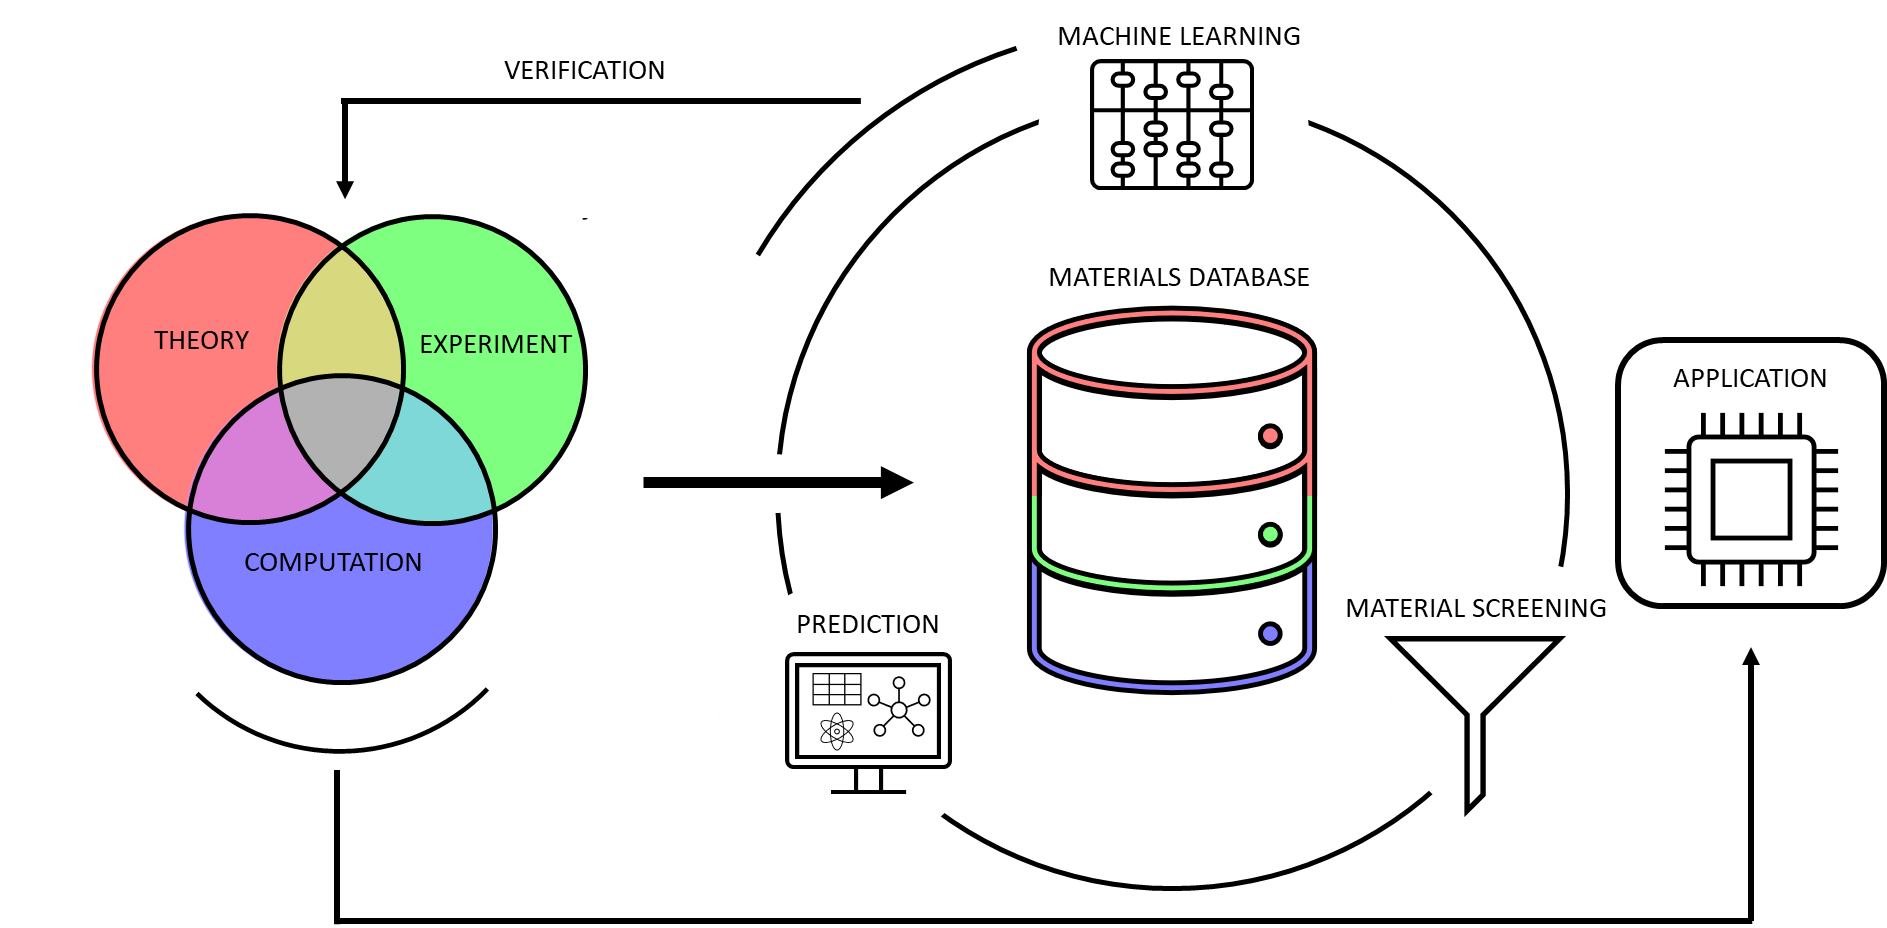
\includegraphics[width=0.9\textwidth]{figures/ht-workflow-new-2.png}
    \caption{Schematic of an example workflow in material informatics. Results from theory, experiment and computation are fed into material databases (arrow pointing to the center). A cycle involving material screening, machine learning and predictions leads to knowledge gain and ultimately applications in fields such as clean energy and quantum technology. 
    }
    \label{fig:ht-workflow}
\end{figure}

Several platforms are available for the development of quantum technologies, but the materials and fabrication technologies are less mature than those for, e.g., classical computers and sensors. 
An important concern in this context is that of scalability. 
For example, the best performing quantum computer prototypes available today rely on superconducting electronics that require millikelvin temperatures to operate, with the stability of interactions between qubits being an important issue. Instead, semiconductors are emerging as a promising alternative platform, offering competitive characteristics combined with the possibility of room temperature operation and mature and scalable material processing and fabrication.  

Quantum technologies based on semiconductors rely on either defects or quantum dots where the latter can be of the self-assembled or nanostructured type \cite{Aharonovich_2016}. 
Semiconductor defects can act as single-photon emitters or spin centers and are compatible with the three main QT categories of computing, communication and sensing \cite{Awschalom_2018}. 
These characteristics are most often found for the case of defects that introduce deep energy levels into the semiconductor band gap \cite{Weber2010}. So-called deep level defects can trap charge carriers in localized states that are essentially isolated from the surroundings, making them highly suitable for QT due to, e.g., indistinguishable single-photon emission and long spin coherence times. 
The most well-known quantum compatible defect is the negatively charged nitrogen-vacancy (NV) center in diamond \cite{Doherty_2013}, but silicon carbide (SiC) and the various quantum emitters therein are strong contenders for quantum communication purposes especially due to the favorable emission wavelength region in the near infrared coupled with more mature material processing and fabrication (see, e.g., Refs.~\cite{Castelletto_2015,Son2020,Bathen2021}). 
However, semiconductor based QT is still in the early stages, and the issues left to address include identification of suitable host materials and candidate defects, and scalable and reproducible quantum device fabrication. 
Furthermore, a complete understanding of the requirements for a semiconductor material to manifest quantum compatible properties \mrk{is lacking},  
and the selection of known quantum compatible host materials is slim \cite{Atatuere2018,Zhang2020}. 

The majority of discoveries of QT compatible characteristics in semiconductors has so far happened by serendipity, and there is an urgent need for a better and more systematic understanding of which material requirements must be met for QT compatible characteristics like single-photon emission and single spin control to manifest. In this context, a framework for dedicated materials search and analysis is needed. 

The fourth science paradigm of big data driven science reveals the potential of targeted search for promising material systems in which to expect QT compatible properties. 
%, see for example Ref.~\cite{Acin2018}.
Rather than searching through a host of signals for those that match our criteria, we aim to \textit{predict} which materials and signatures \mrk{should be targeted} for more detailed studies, following the framework illustrated in Fig.~\ref{fig:ht-workflow}. 
This is made feasible by the availability of databases containing material properties for a wide range of different systems. In this work, the data in question are provided by bulk density functional theory (DFT) calculations to obtain the ground state properties of different elements and compounds. Combined with machine learning (ML) methods we provide a path towards precise classification of candidate materials. The inclusion of ML methods follows recent trends in applications of statistical learning, data science and machine learning for scientific discoveries, see for example Refs.~\cite{deiana2021,Carleo2019}. 

Here we provide a framework for the data mining and automated discovery of promising \mrk{semiconductor hosts for QT} using targeted database search and ML methods combined with knowledge from the field. 
Analyzing the output of the ML methods reveals that, given a suitable initial set of labeled materials for training and testing, it is possible to discern the physical mechanisms that govern a material's suitability for quantum applications.  
In this framework we do not distinguish between the specific mechanism giving rise to properties such as single-photon emission and long spin coherence times (e.g., semiconductor defects or quantum dots); instead, we attempt to target all materials that may accommodate the desired characteristics.  
The methodology developed herein can be modified for other material types and application areas provided that high quality databases containing relevant theoretical and/or experimental data are available. 

The developed procedure relies on data extraction from the databases Materials Project \cite{Jain2013,Jain2018}, the Open Quantum Materials Database (OQMD) \cite{Saal2013, Kirklin2015}, JARVIS-DFT \cite{Choudhary2020}, AFLOW \cite{Curtarolo2012, Curtarolo2012a, Calderon2015} and AFLOW-ML \cite{Isayev2017}. 
The Matminer Python library for data mining \cite{Ward2018} was then used for material analysis to featurize the extracted data. An important aspect of \mrk{the} work is the database building and pertinent development of the datasets for the ML methods. \mrk{Three different approaches to data mining were devised}: (i) \emph{the Ferrenti approach} which is similar to that proposed by \citeauthor{Ferrenti2020} \cite{Ferrenti2020}, (ii) \emph{the extended Ferrenti approach} and (iii) \emph{the empirical approach}. \mrk{The} two first methodologies base their data extraction protocols on broad material descriptors, leading to large sets of potentially suitable candidates \cite{Mehta2019,Hastie2009}. The empirical approach, on the other hand, relies on including materials with experimentally proven advantageous characteristics in the training set and therefore yields a narrower set of possible candidates. The three resulting sets of labeled data were then analyzed with the four supervised ML methods logistic regression, decision trees, random forests and gradient boosting \cite{Hastie2009,Murphy2012}, yielding \mrk{$47$} predicted candidates that were common between all approaches and ML methods.  
Example materials \mrk{among the predictions} include ZnGeP$_2$, CdS, BP, BC$_2$N, GeC and InP. Focused theoretical and experimental studies, using methods such as, e.g., density functional theory, photoluminescence spectroscopy and optically detected magnetic resonance, are needed to verify the predictions that quantum properties may manifest as a result of defects or nanostructures in the above listed materials. 
%Write better! 
Importantly, our findings also reveal which material properties are weighted by the ML methods upon predicting a material as suitable for QT applications, thereby opening up for new  discoveries in the field of quantum technologies. 


\section*{Results}

\subsection*{Information Flow} 

The information stream in this work can be regarded as many inter-connected modular parts. 
The initial step for gathering material data and building features is visualized by the outer flowchart in Fig.~\ref{fig:flowchart} (Jupyter notebooks containing the full 
workflow can be found at \cite{Ohebbi2021}).
We start by extracting all entries in the Materials Project (MP) database  \cite{Jain2013,Jain2018} that match a specific query. 
The MP database contains ground state properties of different materials that are computed using density functional theory. The DFT calculations in the database were performed using the Vienna {\em ab initio} simulation package (VASP) \cite{Kresse1996} and the Perdew-Burke-Ernzerhof (PBE) \cite{Perdew1996} exchange-correlation functional to calculate the electronic structure of the materials. 
We note that despite being immensely successful in describing a number of material properties, PBE is widely known for underestimating the band gap of semiconductors \cite{Freysoldt2014}. Therefore, not all properties predicted using the PBE functional are reliable, and the band gaps in particular cannot be trusted in absolute terms. Nonetheless, the functional is in wide use due to the combination of reasonable accuracy and high computational throughput, and is usually considered to be reliable for large-scale trends in semiconductor \mrk{material} properties. 

\begin{figure}[t]
    \centering
    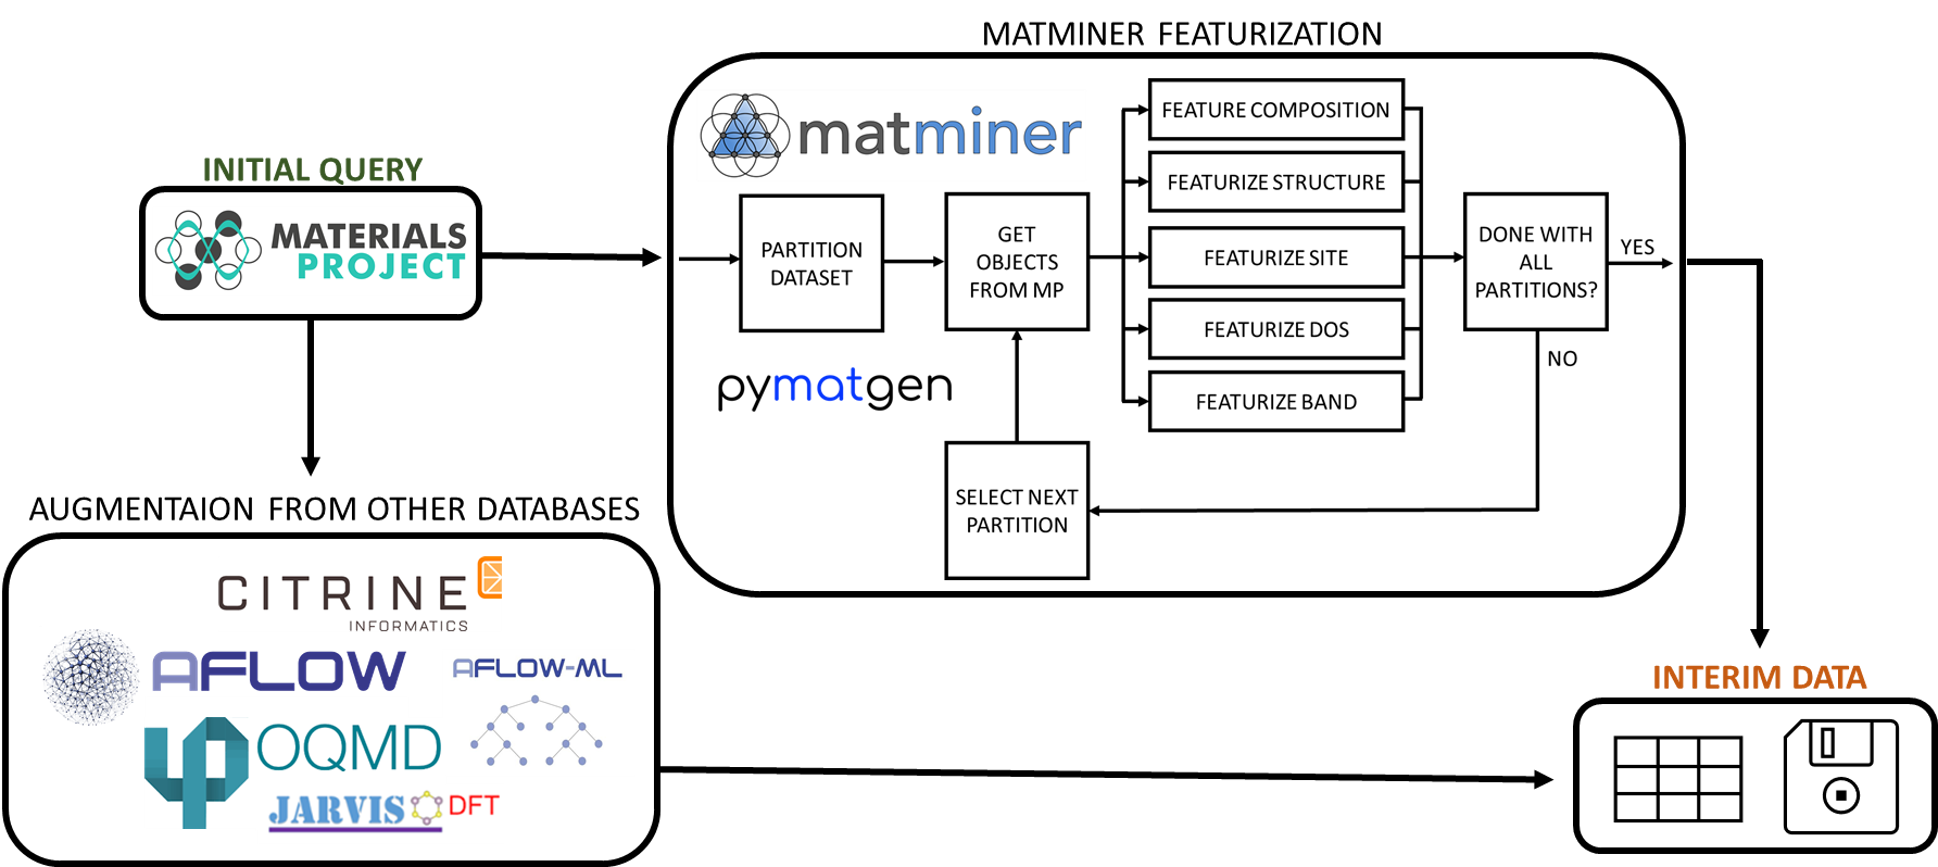
\includegraphics[width=0.9\textwidth]{figures/flow_chart_2.png}
    \caption{The project workflow starting from an initial Materials Project (MP) query, and ending with a featurized dataset with entries from several other databases. 
    To limit the memory and computational usage, the data are partitioned into smaller subsets where the respective Pymatgen objects (Pymatgen is a robust, open-source Python library for materials analysis \cite{pymatgen}) are obtained through a query to be used in the following featurization steps. This process is repeated iteratively until all the data has been featurized. \emph{DOS} refers to density of states and \emph{band} to the electronic band structure. 
    }
    \label{fig:flowchart}
\end{figure}

The conditions for the initial MP query are that the materials must derive from the Inorganic Crystal Structure Database (ICSD) and have a band gap wider than $0.1$~eV to exclude metallic compounds. The ICSD is the world's largest database for completely identified inorganic crystal structures  \cite{Allen1987,Zagorac2019}. In a parallel step, entries that are deemed similar to the entries from the initial query are extracted from the databases OQMD  \cite{Saal2013,Kirklin2015}, JARVIS-DFT \cite{Choudhary2020}, AFLOW \cite{Curtarolo2012, Curtarolo2012a, Calderon2015}, AFLOW-ML \cite{Isayev2017} and the Citrination platform \cite{OMaraJordan2016MDIA}. The results of these steps are combined into a dataset for further analysis. 

After material extraction we apply tools from the open-source library Matminer \cite{Ward2018} to generate thousands of features from the data. We will refer to this process as featurization. A schematic visualization of the featurization process in Matminer is shown in  Fig.~\ref{fig:flowchart} 
and focuses on a material's composition,  structure, atomic sites, density of states and band structure. 
The $39$ featurizers (each generates several features) selected as material descriptors in this work are \mrk{described} in the Supplementary Information at \cite{supplementary}. The selection of features was kept rather wide \mrk{to avoid making} {\em ex ante} assumptions on which features best describe a solid state material platform for \mrk{QT}. 

The constructed dataset encompasses compounds formed by a plethora of combinations of surfaces, interfaces, nanostructures, compositions and structures, but this complexity is not necessarily reflected in the material descriptors. 
Furthermore, we have utilized data obtained from high-throughput density functional theory calculations. Indeed, there are possible errors associated with every step, starting from an initial calculation, adding of data in the database, gathering of data, featurization of data, preprocessing of data, data mining, and finally training a model and making a prediction. Unfortunately, if an error has \mrk{occurred} in the first part of the process, the error \mrk{is carried along} and will get increasingly harder to detect. Thus, \mrk{the} results depend on the quality of data in the \mrk{employed} databases. 

\subsection*{Data Mining}
The complete dataset consists of \mrk{$25,000$} materials. A subset of these materials is labeled into either suitable or unsuitable candidates for QT while the remainder will stay unlabeled. The labeled data are then grouped into training and test sets for the ML methods.
\mrk{The ML methods are trained using the training set and then evaluated on the test set.}
\mrk{Finally, the ML methods are applied to the unlabeled data for which predictions of QT suitability are made.}

Several challenges accompany the labeling \mrk{process.} 
%of labeling materials according to their suitability for QT. 
Although QT compatible properties are becoming increasingly well studied for the case of, e.g., nitrogen-vacancy centers in diamond, single-photon emitters in silicon carbide and quantum dot (QD) structures \cite{Doherty_2013,Bathen2021,Aharonovich_2016}, relatively few candidate materials are known to be suitable  \cite{Atatuere2018,Zhang2020}. An additional consideration is that the physical mechanisms promoting favorable properties are not fully understood. 
Conversely, defining materials as unsuitable candidates for QT is in many ways equally difficult, as the mechanisms preventing quantum compatible characteristics to manifest are \mrk{not known either}.  
The strategy for selection of unsuitable candidates is thus that the negation of the criteria \mrk{used} to select suitable candidates should give unsuitable candidates.
A side-effect of this selection is that the criteria for unsuitable candidates can become equally, or more, restrictive compared to the criteria for suitable candidates\mrk{, resulting in} skewed data sets \mrk{with} fewer unsuitable than suitable candidates. 
This method for selecting unsuitable candidates has shortcomings but will serve as a starting point and demonstration for how the labeling procedure could be improved. 
Below \mrk{three separate procedures for labeling materials as suitable or unsuitable candidates for QT are described}. 

\subsubsection*{The Ferrenti approach}
The first approach to labeling a selection of materials in the dataset is based on the criteria proposed by \citeauthor{Ferrenti2020} \cite{Ferrenti2020}. 
They suggest a data mining process consisting of four stages by systematically evaluating the suitability of host materials taken from the Materials Project. 
\mrk{Note that the data mining process in Ref.~\cite{Ferrenti2020} alone was intended for further experimental studies and not necessarily for a targeted machine learning search. Nonetheless, we adapt the selection criteria from Ref.~\cite{Ferrenti2020} for the present purposes.}
In the \mrk{\emph{Ferrenti approach}} framework, \textbf{suitable} candidates \mrk{are labeled} by the following steps: 
\begin{enumerate}
    \item Include materials that;
    \begin{itemize}
        \item contain elements with more than $50 \ \%$ natural abundance of spin zero isotopes,
        \item crystallize in non-polar space groups,
        \item are present in the ICSD\mrk{,} 
        and
        \item are calculated to be nonmagnetic. 
    \end{itemize}
    \item Pragmatically remove toxic, radioactive and otherwise ``difficult'' materials;
    \begin{itemize}
        \item exclude Th, U, Cd and Hg because they are radioactive and/or toxic in the most stable forms,
        \item exclude any rare-earth metals (because of the difficulty of obtaining pure materials free of isotopes with nuclear spin) and noble gases (due to the lack of stable solid phases),
        \item exclude transition metal elements with unpaired electrons like Fe and Ni because of their paramagnetism; Ru and Os are also excluded because they only exist in the dataset as complex cluster structures. 
    \end{itemize}
    \item Include only materials with a band gap larger than $0.5$~eV calculated using DFT and the PBE functional. The value of $0.5$~eV was chosen to match that typically predicted for silicon by PBE-level DFT calculations. 
    \item Ensure that the energy above hull is less than $0.2$~eV per atom.
\end{enumerate}

These inclusion criteria are based on the work of \citeauthor{Weber2010} \cite{Weber2010} and targeted primarily at semiconductors that can host deep level defects with spin qubit capabilities. In this context, long spin coherence times are needed, \mrk{necessitating an environment that can be depleted of nuclear spins and permanent magnetism.} 
%and the possibility of having an environment free of nuclear spins and permanent magnetism is therefore desirable. 
Moreover, non-polar materials are assumed to be preferable to obtain \mrk{sharp and indistinguishable single-photon emission from defects}.  
Transition metal elements are eliminated if they have unpaired electrons because the presence of permanent electric dipole moments may have a detrimental impact on the optical coherence of defect emission. 
Finally, the energy above hull requirement \mrk{ensures} that the selected compounds are thermodynamically stable.
\mrk{Note that larger cells are sometimes needed to verify antiferromagnetic ordering so the criteria mainly target ferromagnetic ordering under the labels magnetic/non-magnetic.}

Next, \textbf{unsuitable} candidates are labeled according to the reverse requirements of the above; as materials in the \mrk{ICSD} that crystallize in polar space groups, are calculated to be magnetic and have a band gap larger than $0.1$~eV in the MP database (to exclude metals but include lower-band gap semiconductors). 
The resulting set of labeled materials contains $1581$ materials where $35 \ \%$
are labeled as unsuitable and 
$65 \ \%$ as suitable for QT applications, \mrk{evidencing that} 
%Here we see the first example of how 
the criteria for labeling unsuitable candidates are more restrictive than those for the suitable candidates.

\mrk{Performing machine learning on a data set derived using preconceived notions for which material properties are important is likely to reproduce several of the initial selection criteria. Nonetheless, the Ferrenti approach was included in the present work to highlight expectations from the literature and contrast them with the findings from the other approaches. Additionally, one should note that ML methods are often capable of recognizing other patterns than those intended for the data, opening up the possibility that also the Ferrenti approach could yield new insights.} 


\subsubsection*{The extended Ferrenti approach}
\mrk{The Ferrenti approach was adjusted} to expand the data labeling process beyond practical  considerations. The second approach is therefore named \emph{the extended Ferrenti approach} and involves removing stage two from the approach above. Moreover, \mrk{certain} additional elements that have shown promising properties but were initially excluded due to the lack of spin zero isotopes \mrk{are also included}. 

The following steps constitute the process of labeling \textbf{suitable} candidates in the \mrk{extended Ferrenti approach}:
\begin{enumerate}
    \item Include materials that; 
    \begin{itemize}
        \item contain elements where more than half have a natural abundance of spin zero isotopes, including Al, P, Ga, As, B and N, 
        \item crystallize in non-polar space groups,
        \mrk{are present in the ICSD,
        and are calculated to be nonmagnetic.} 
    \end{itemize}
    \item Only keep materials that have a band gap larger than $1.5$~eV in the MP database. The higher band gap requirement (as compared to the Ferrenti approach) is included here to avoid labeling an unfeasibly large number of materials. 
    \item Ensure that the energy above hull is less than $0.2$~eV per atom. 
\end{enumerate}

For \textbf{unsuitable} candidates, \mrk{the same strategy as for the Ferrenti approach was implemented}. The result is \mrk{an} unbalanced set of labeled materials with up to $75 \ \%$ of the materials found in the suitable group \mrk{and $78 \ \%$ more materials than for the Ferrenti approach.} 
%However, the labeled data encompasses $78 \ \%$ more materials than  the Ferrenti approach, consisting of $2141$ suitable and $684$ unsuitable materials.

\mrk{The findings from both the data mining and machine learning procedures for the extended Ferrenti approach did not differ substantially from those obtained using the Ferrenti approach. This is attributed to the similarities in the selection processes. Therefore, detailed discussion on the findings from the extended Ferrenti approach can be found in the Supplementary Information at \cite{supplementary}. Qualitative conclusions drawn for the Ferrenti approach herein also hold for the extended Ferrenti approach, indicating that the removal of so-called practical considerations did not have a significant impact on the results. }

\subsubsection*{The empirical approach}
%The third approach differs substantially from the others in terms of material labeling, as 
\mrk{In the \emph{empirical approach},} we apply knowledge from the field (see for instance  Refs.~\cite{Atatuere2018,Toth2019,Zhang2020,Son2020} for an overview) to \mrk{guide the search for} promising material \mrk{hosts.}  
In other words, \mrk{the labeled data contains candidates} where quantum compatible properties have been either experimentally demonstrated or theoretically predicted\mrk{, including the materials suggested in Ref.~\cite{Weber2010} as promising deep level defect hosts.} 
%We therefore name this scheme \emph{the empirical approach}. 
%Due to the concern of ending up with too small datasets for training and testing of the ML methods, we will also include some  materials that are promising in the sense that they have suitable properties for accommodating deep level defects that can potentially exhibit quantum effects --- even though such effects may not yet have been shown. 
%These material choices were motivated by the criteria and predictions for QT compatible deep level defects defined by \citeauthor{Weber2010} \cite{Weber2010}. 
%\mrk{The theoretical predictions were motivated by the criteria for having deep level defects exhibit quantum compatible properties \cite{Weber2010}.} 
%material choices were motivated by the criteria and predictions for QT compatible deep level defects defined by \citeauthor{Weber2010} \cite{Weber2010}. 
\mrk{Materials where single-photon emission and spin manipulation have been observed but attributed to excitonic effects or quantum dots (formed by self-assembly or lithographic structuring) rather than being defect related were also included.} 


Table~\ref{tab:qt-materials} contains an overview of known semiconductor materials with demonstrated quantum compatible characteristics. The table forms the basis for picking suitable candidates for the empirical approach. The properties being studied arise from mechanisms related to, e.g., point defects, bound excitons, and both self-assembled and lithographically structured quantum dots and nanostructures such as 2D materials. 
Quantum emission signatures have been assigned to specific defects in both diamond and SiC, but for most other materials, secure identification of the responsible defects or structure related mechanism is still lacking.  

The strategy for picking \textbf{suitable} candidates in the empirical approach can be summed up as;  
\begin{enumerate}
    \item Select candidate materials that match the formulas in  Table~\ref{tab:qt-materials}, or the formulas ZnSe, AlP, GaP, AlAs, ZnTe, CdS \cite{Weber2010} and SiGe \cite{Hardy2019}, as these materials have been predicted to behave as suitable quantum hosts based on favorable properties such as a wide band gap and low spin-orbit coupling.  
    \item Ensure that the candidates are present in the ICSD.  
    \item Perform a manual screening for appropriate crystallographic structures. 
\end{enumerate}

\begin{table}[t]
    \centering 
    \caption{Overview of materials and defects that have been demonstrated to exhibit quantum  compatible characteristics such as single-photon emission and coherent spin manipulation. The subscript denotes lattice site and $V$ refers to a vacancy. }
    \begin{tabular}{c|c|c|c}
    Material & Band gap (eV) & Defect candidates & References \\
    \hline
    Diamond  & $5.5$  & N$_\mathrm{C}V_\mathrm{C}$, Si$_\mathrm{C}V_\mathrm{C}$, Ge$_\mathrm{C}V_\mathrm{C}$ & \cite{Taylor2008,Balasubramanian_2009,Barclay2011,Gordon2013,Rogers_2014,Bhaskar_2018} \\ 
    SiC & $2.2$-$3.3$ & $V_\mathrm{Si}$, $V_\mathrm{Si}V_\mathrm{C}$, C$_\mathrm{Si}V_\mathrm{C}$, N$_\mathrm{C}V_\mathrm{Si}$ & \cite{Widmann2014,Christle_2015,Castelletto_2014,Zargaleh_2018}  \cite{Weber2010, Son2020, Falk2013} \\ 
    Si & $1.1$ & P, G, unidentified & \cite{Muhonen_2014,Durand_2020,Redjem2020} \\ 
    (2D) \textit{h}-BN & $6.0$ & Unidentified defects & \cite{Tran_2016,Tran_2016b,Hayee_2020} \\ 
    (2D) MoS$_2$, WSe$_2$, WS$_2$ & $<2.5$~eV & Bound excitons & \cite{Toth2019} \\
    ZnO & $3.4$ & Unidentified defects & \cite{Morfa2012} \\ 
    ZnS & $3.6$ (zincblende) & Unidentified defects & \cite{Stewart2019} \\ 
    GaAs & $1.4$ & Quantum dots & \cite{Bluhm2010} \\ 
    GaN & $3.4$ & Quantum dots, unidentified defects & \cite{Roux2017,Berhane2018} \\
    AlN & $6.0$ & Unidentified defects & \cite{Xue2020}\\
    \end{tabular}
    \label{tab:qt-materials}
\end{table} 

After the first stage of picking candidates we are left with a list of $202$ matching formulas which includes $12$ entries that have a band gap of less than $0.4$~eV. These $12$ entries are calculated to be thermodynamically unstable in terms of the energy above hull, and will decompose into other materials in the list --- incidentally, the resulting structures all have calculated band gaps that are substantially larger than $0.5$~eV. \mrk{All of the $202$ structures are included apart from C (mp-$568410$) which is a metal according to AFLOW-ML. }
 

Entries matching the formulas C, SiC, BN, MoS$_2$, WSe$_2$ and WS$_2$ (quantum compatible characteristics have been demonstrated) were manually screened to see whether they have a matching structure to the respective candidates discussed earlier and summarized in Table~\ref{tab:qt-materials}. 
For carbon, three-dimensional diamond-like structures as explicitly stated in the column tags from the Materials Project \mrk{were admitted.} Additionally, we find several two-dimensional structures of carbon with a large band gap ($>1.5$~eV) among the data. \mrk{These were added} as suitable candidates. Complex structures (e.g., C$_{28}$, C$_{48}$ and C$_{60}$) were moved to the test set in our machine learning studies. For SiC we admitted all entries which included the $2$H, $3$C, $4$H, $6$H and $15$R polytypes. Concerning BN, MoS$_2$, WSe$_2$ and WS$_2$, \mrk{only two-dimensional structures were admitted}. For non-matching structures not mentioned so far, we move them to the test set to see if they will be predicted as suitable or not by the ML methods that are applied in a later stage.

The materials AlP, GaP, AlAs, ZnTe and CdS were manually screened for tetrahedrally coordinated structures, and have been included since \citeauthor{Weber2010} \cite{Weber2010} identified them as potentially promising candidates due to suitable material properties. 
\mrk{Note} that only tetrahedrally coordinated structures of the given formulas were labeled as suitable after imposing a band gap restriction of $0.5$~eV. 

Following the three screening steps in the empirical approach, a total of $187$ entries were labeled as suitable candidates for the training set. 
Notably, the candidates labeled as suitable in the empirical approach contain only compounds that are either elementary (unary) or binary. 
Since the set of labeled data constituting suitable candidates in the empirical approach contains rather few entries, \mrk{$400$ materials were added and labeled as \textbf{unsuitable}}. These \mrk{were} picked at random from the pool of unsuitable candidates from the two previous approaches, in addition to those that were marked as unsuitable during the manual screening process. 

\subsubsection*{Comparing the approaches}
%The three different approaches to data mining place a particular emphasis on each of their specific goals. The Ferrenti approach relies on choosing only elements with spin zero isotopes and compounds that crystallize in nonpolar spacegroups together with practical filters, while the extended Ferrenti approach allows a larger variety of elements and removes the practical reasons for excluding candidate materials. Thus, the first approach targets a more narrow prediction space than the second approach does. However, the most selective approach is the empirical one, relying exclusively on previous findings rather than assuming which material properties are influential. 

 
%Ferrenti 
\mrk{Considering the materials present in the labeled datasets of the Ferrenti approach more closely, we find that carbon in a diamond-like structure is classified as a suitable candidate}, in good agreement with experimental observations (see Table~\ref{tab:qt-materials}). Interestingly, in the labeled data from the Ferrenti approach, we find that carbon in two-dimensional graphite-like structures are marked as suitable as well. All structures of silicon are also labeled as suitable together with one entry of silicon carbide. Note that this is the $3$C polytype of SiC, meaning that the most well-established quantum compatible SiC polytype, $4$H-SiC, is missing. 
Among other potentially suitable candidates we find ZnS, ZnSe, ZnO and ZnTe present in the labeled data from the Ferrenti approach.  
%Extended Ferrenti - moved 
%In the labeled dataset of the extended Ferrenti approach, we find a single entry for each of SiC, Si, GaN, ZnS, GaP, AlAs and AlP, carbon in both diamond- and graphite-like structures, and AlN in three different configurations. The labeled dataset includes a larger variety of materials that are known to be quantum compatible as compared to the Ferrenti approach due to admitting more elements in the initial selection process. However, since we also included a more stringent band gap restriction of $1.5$~eV (to reduce the amount of materials in the training set), there is a more sparse representation of each known chemical formula present in the labeled data.

\mrk{The labeled data for the Ferrenti and empiricial approaches is visualized in Figure~\ref{fig:parallel-coordinates-approaches}} as parallel coordinate plots for a few selected features informed by the criteria proposed by \citeauthor{Weber2010} \cite{Weber2010}. Parallel coordinate schemes  \cite{Inselberga1990, Inselberg1985} represent a multi-dimensional data tuple as one polyline crossing a parallel axis. The selected features are found on the $x$-axis, while the $y$-axis shows the value of the data. Thus, parallel coordinate plots can turn complex many-dimensional data into a compact  two-dimensional representation. Due to possible data cluttering, the figure visualizes a random sample of each class (suitable or unsuitable) with an upper limit of $250$ per class with transparent lines. The green and red polylines represent suitable and unsuitable candidates, respectively. 

\begin{figure}[t] %!htp
    \centering
    \begin{subfigure}{1\textwidth}
        \centering
        \scalebox{0.85}{%% Creator: Matplotlib, PGF backend
%%
%% To include the figure in your LaTeX document, write
%%   \input{<filename>.pgf}
%%
%% Make sure the required packages are loaded in your preamble
%%   \usepackage{pgf}
%%
%% and, on pdftex
%%   \usepackage[utf8]{inputenc}\DeclareUnicodeCharacter{2212}{-}
%%
%% or, on luatex and xetex
%%   \usepackage{unicode-math}
%%
%% Figures using additional raster images can only be included by \input if
%% they are in the same directory as the main LaTeX file. For loading figures
%% from other directories you can use the `import` package
%%   \usepackage{import}
%%
%% and then include the figures with
%%   \import{<path to file>}{<filename>.pgf}
%%
%% Matplotlib used the following preamble
%%   \usepackage[detect-all,locale=DE]{siunitx} \usepackage[T1]{fontenc} \usepackage[utf8x]{inputenc}
%%
\begingroup%
\makeatletter%
\begin{pgfpicture}%
\pgfpathrectangle{\pgfpointorigin}{\pgfqpoint{5.584949in}{2.190539in}}%
\pgfusepath{use as bounding box, clip}%
\begin{pgfscope}%
\pgfsetbuttcap%
\pgfsetmiterjoin%
\pgfsetlinewidth{0.000000pt}%
\definecolor{currentstroke}{rgb}{1.000000,1.000000,1.000000}%
\pgfsetstrokecolor{currentstroke}%
\pgfsetstrokeopacity{0.000000}%
\pgfsetdash{}{0pt}%
\pgfpathmoveto{\pgfqpoint{0.000000in}{0.000000in}}%
\pgfpathlineto{\pgfqpoint{5.584949in}{0.000000in}}%
\pgfpathlineto{\pgfqpoint{5.584949in}{2.190539in}}%
\pgfpathlineto{\pgfqpoint{0.000000in}{2.190539in}}%
\pgfpathclose%
\pgfusepath{}%
\end{pgfscope}%
\begin{pgfscope}%
\pgfsetbuttcap%
\pgfsetmiterjoin%
\definecolor{currentfill}{rgb}{1.000000,1.000000,1.000000}%
\pgfsetfillcolor{currentfill}%
\pgfsetlinewidth{0.000000pt}%
\definecolor{currentstroke}{rgb}{0.000000,0.000000,0.000000}%
\pgfsetstrokecolor{currentstroke}%
\pgfsetstrokeopacity{0.000000}%
\pgfsetdash{}{0pt}%
\pgfpathmoveto{\pgfqpoint{0.377421in}{0.128033in}}%
\pgfpathlineto{\pgfqpoint{5.264131in}{0.128033in}}%
\pgfpathlineto{\pgfqpoint{5.264131in}{1.607731in}}%
\pgfpathlineto{\pgfqpoint{0.377421in}{1.607731in}}%
\pgfpathclose%
\pgfusepath{fill}%
\end{pgfscope}%
\begin{pgfscope}%
\pgfpathrectangle{\pgfqpoint{0.377421in}{0.128033in}}{\pgfqpoint{4.886710in}{1.479697in}}%
\pgfusepath{clip}%
\pgfsetbuttcap%
\pgfsetmiterjoin%
\pgfsetlinewidth{0.501875pt}%
\definecolor{currentstroke}{rgb}{1.000000,0.388235,0.278431}%
\pgfsetstrokecolor{currentstroke}%
\pgfsetstrokeopacity{0.200000}%
\pgfsetdash{}{0pt}%
\pgfpathmoveto{\pgfqpoint{0.377421in}{1.540472in}}%
\pgfpathcurveto{\pgfqpoint{0.703201in}{1.540472in}}{\pgfqpoint{1.028982in}{0.255216in}}{\pgfqpoint{1.354763in}{0.255216in}}%
\pgfpathcurveto{\pgfqpoint{1.680543in}{0.255216in}}{\pgfqpoint{2.006324in}{0.891527in}}{\pgfqpoint{2.332105in}{0.891527in}}%
\pgfpathcurveto{\pgfqpoint{2.657886in}{0.891527in}}{\pgfqpoint{2.983666in}{0.921833in}}{\pgfqpoint{3.309447in}{0.921833in}}%
\pgfpathcurveto{\pgfqpoint{3.635228in}{0.921833in}}{\pgfqpoint{3.961008in}{1.271436in}}{\pgfqpoint{4.286789in}{1.271436in}}%
\pgfpathcurveto{\pgfqpoint{4.612570in}{1.271436in}}{\pgfqpoint{4.938350in}{0.969293in}}{\pgfqpoint{5.264131in}{0.969293in}}%
\pgfusepath{stroke}%
\end{pgfscope}%
\begin{pgfscope}%
\pgfpathrectangle{\pgfqpoint{0.377421in}{0.128033in}}{\pgfqpoint{4.886710in}{1.479697in}}%
\pgfusepath{clip}%
\pgfsetbuttcap%
\pgfsetmiterjoin%
\pgfsetlinewidth{0.501875pt}%
\definecolor{currentstroke}{rgb}{1.000000,0.388235,0.278431}%
\pgfsetstrokecolor{currentstroke}%
\pgfsetstrokeopacity{0.200000}%
\pgfsetdash{}{0pt}%
\pgfpathmoveto{\pgfqpoint{0.377421in}{1.540472in}}%
\pgfpathcurveto{\pgfqpoint{0.703201in}{1.540472in}}{\pgfqpoint{1.028982in}{0.210041in}}{\pgfqpoint{1.354763in}{0.210041in}}%
\pgfpathcurveto{\pgfqpoint{1.680543in}{0.210041in}}{\pgfqpoint{2.006324in}{0.518210in}}{\pgfqpoint{2.332105in}{0.518210in}}%
\pgfpathcurveto{\pgfqpoint{2.657886in}{0.518210in}}{\pgfqpoint{2.983666in}{0.792350in}}{\pgfqpoint{3.309447in}{0.792350in}}%
\pgfpathcurveto{\pgfqpoint{3.635228in}{0.792350in}}{\pgfqpoint{3.961008in}{0.733364in}}{\pgfqpoint{4.286789in}{0.733364in}}%
\pgfpathcurveto{\pgfqpoint{4.612570in}{0.733364in}}{\pgfqpoint{4.938350in}{0.205942in}}{\pgfqpoint{5.264131in}{0.205942in}}%
\pgfusepath{stroke}%
\end{pgfscope}%
\begin{pgfscope}%
\pgfpathrectangle{\pgfqpoint{0.377421in}{0.128033in}}{\pgfqpoint{4.886710in}{1.479697in}}%
\pgfusepath{clip}%
\pgfsetbuttcap%
\pgfsetmiterjoin%
\pgfsetlinewidth{0.501875pt}%
\definecolor{currentstroke}{rgb}{1.000000,0.388235,0.278431}%
\pgfsetstrokecolor{currentstroke}%
\pgfsetstrokeopacity{0.200000}%
\pgfsetdash{}{0pt}%
\pgfpathmoveto{\pgfqpoint{0.377421in}{1.540472in}}%
\pgfpathcurveto{\pgfqpoint{0.703201in}{1.540472in}}{\pgfqpoint{1.028982in}{0.299886in}}{\pgfqpoint{1.354763in}{0.299886in}}%
\pgfpathcurveto{\pgfqpoint{1.680543in}{0.299886in}}{\pgfqpoint{2.006324in}{0.518210in}}{\pgfqpoint{2.332105in}{0.518210in}}%
\pgfpathcurveto{\pgfqpoint{2.657886in}{0.518210in}}{\pgfqpoint{2.983666in}{1.396602in}}{\pgfqpoint{3.309447in}{1.396602in}}%
\pgfpathcurveto{\pgfqpoint{3.635228in}{1.396602in}}{\pgfqpoint{3.961008in}{0.733364in}}{\pgfqpoint{4.286789in}{0.733364in}}%
\pgfpathcurveto{\pgfqpoint{4.612570in}{0.733364in}}{\pgfqpoint{4.938350in}{0.229818in}}{\pgfqpoint{5.264131in}{0.229818in}}%
\pgfusepath{stroke}%
\end{pgfscope}%
\begin{pgfscope}%
\pgfpathrectangle{\pgfqpoint{0.377421in}{0.128033in}}{\pgfqpoint{4.886710in}{1.479697in}}%
\pgfusepath{clip}%
\pgfsetbuttcap%
\pgfsetmiterjoin%
\pgfsetlinewidth{0.501875pt}%
\definecolor{currentstroke}{rgb}{1.000000,0.388235,0.278431}%
\pgfsetstrokecolor{currentstroke}%
\pgfsetstrokeopacity{0.200000}%
\pgfsetdash{}{0pt}%
\pgfpathmoveto{\pgfqpoint{0.377421in}{1.540472in}}%
\pgfpathcurveto{\pgfqpoint{0.703201in}{1.540472in}}{\pgfqpoint{1.028982in}{0.299946in}}{\pgfqpoint{1.354763in}{0.299946in}}%
\pgfpathcurveto{\pgfqpoint{1.680543in}{0.299946in}}{\pgfqpoint{2.006324in}{1.325605in}}{\pgfqpoint{2.332105in}{1.325605in}}%
\pgfpathcurveto{\pgfqpoint{2.657886in}{1.325605in}}{\pgfqpoint{2.983666in}{1.130444in}}{\pgfqpoint{3.309447in}{1.130444in}}%
\pgfpathcurveto{\pgfqpoint{3.635228in}{1.130444in}}{\pgfqpoint{3.961008in}{1.002400in}}{\pgfqpoint{4.286789in}{1.002400in}}%
\pgfpathcurveto{\pgfqpoint{4.612570in}{1.002400in}}{\pgfqpoint{4.938350in}{0.842391in}}{\pgfqpoint{5.264131in}{0.842391in}}%
\pgfusepath{stroke}%
\end{pgfscope}%
\begin{pgfscope}%
\pgfpathrectangle{\pgfqpoint{0.377421in}{0.128033in}}{\pgfqpoint{4.886710in}{1.479697in}}%
\pgfusepath{clip}%
\pgfsetbuttcap%
\pgfsetmiterjoin%
\pgfsetlinewidth{0.501875pt}%
\definecolor{currentstroke}{rgb}{1.000000,0.388235,0.278431}%
\pgfsetstrokecolor{currentstroke}%
\pgfsetstrokeopacity{0.200000}%
\pgfsetdash{}{0pt}%
\pgfpathmoveto{\pgfqpoint{0.377421in}{1.540472in}}%
\pgfpathcurveto{\pgfqpoint{0.703201in}{1.540472in}}{\pgfqpoint{1.028982in}{0.509186in}}{\pgfqpoint{1.354763in}{0.509186in}}%
\pgfpathcurveto{\pgfqpoint{1.680543in}{0.509186in}}{\pgfqpoint{2.006324in}{1.352950in}}{\pgfqpoint{2.332105in}{1.352950in}}%
\pgfpathcurveto{\pgfqpoint{2.657886in}{1.352950in}}{\pgfqpoint{2.983666in}{0.914639in}}{\pgfqpoint{3.309447in}{0.914639in}}%
\pgfpathcurveto{\pgfqpoint{3.635228in}{0.914639in}}{\pgfqpoint{3.961008in}{1.002400in}}{\pgfqpoint{4.286789in}{1.002400in}}%
\pgfpathcurveto{\pgfqpoint{4.612570in}{1.002400in}}{\pgfqpoint{4.938350in}{0.655862in}}{\pgfqpoint{5.264131in}{0.655862in}}%
\pgfusepath{stroke}%
\end{pgfscope}%
\begin{pgfscope}%
\pgfpathrectangle{\pgfqpoint{0.377421in}{0.128033in}}{\pgfqpoint{4.886710in}{1.479697in}}%
\pgfusepath{clip}%
\pgfsetbuttcap%
\pgfsetmiterjoin%
\pgfsetlinewidth{0.501875pt}%
\definecolor{currentstroke}{rgb}{1.000000,0.388235,0.278431}%
\pgfsetstrokecolor{currentstroke}%
\pgfsetstrokeopacity{0.200000}%
\pgfsetdash{}{0pt}%
\pgfpathmoveto{\pgfqpoint{0.377421in}{1.540472in}}%
\pgfpathcurveto{\pgfqpoint{0.703201in}{1.540472in}}{\pgfqpoint{1.028982in}{0.255078in}}{\pgfqpoint{1.354763in}{0.255078in}}%
\pgfpathcurveto{\pgfqpoint{1.680543in}{0.255078in}}{\pgfqpoint{2.006324in}{1.313398in}}{\pgfqpoint{2.332105in}{1.313398in}}%
\pgfpathcurveto{\pgfqpoint{2.657886in}{1.313398in}}{\pgfqpoint{2.983666in}{0.475838in}}{\pgfqpoint{3.309447in}{0.475838in}}%
\pgfpathcurveto{\pgfqpoint{3.635228in}{0.475838in}}{\pgfqpoint{3.961008in}{0.733364in}}{\pgfqpoint{4.286789in}{0.733364in}}%
\pgfpathcurveto{\pgfqpoint{4.612570in}{0.733364in}}{\pgfqpoint{4.938350in}{0.534807in}}{\pgfqpoint{5.264131in}{0.534807in}}%
\pgfusepath{stroke}%
\end{pgfscope}%
\begin{pgfscope}%
\pgfpathrectangle{\pgfqpoint{0.377421in}{0.128033in}}{\pgfqpoint{4.886710in}{1.479697in}}%
\pgfusepath{clip}%
\pgfsetbuttcap%
\pgfsetmiterjoin%
\pgfsetlinewidth{0.501875pt}%
\definecolor{currentstroke}{rgb}{1.000000,0.388235,0.278431}%
\pgfsetstrokecolor{currentstroke}%
\pgfsetstrokeopacity{0.200000}%
\pgfsetdash{}{0pt}%
\pgfpathmoveto{\pgfqpoint{0.377421in}{1.540472in}}%
\pgfpathcurveto{\pgfqpoint{0.703201in}{1.540472in}}{\pgfqpoint{1.028982in}{0.225185in}}{\pgfqpoint{1.354763in}{0.225185in}}%
\pgfpathcurveto{\pgfqpoint{1.680543in}{0.225185in}}{\pgfqpoint{2.006324in}{1.028930in}}{\pgfqpoint{2.332105in}{1.028930in}}%
\pgfpathcurveto{\pgfqpoint{2.657886in}{1.028930in}}{\pgfqpoint{2.983666in}{0.900253in}}{\pgfqpoint{3.309447in}{0.900253in}}%
\pgfpathcurveto{\pgfqpoint{3.635228in}{0.900253in}}{\pgfqpoint{3.961008in}{0.733364in}}{\pgfqpoint{4.286789in}{0.733364in}}%
\pgfpathcurveto{\pgfqpoint{4.612570in}{0.733364in}}{\pgfqpoint{4.938350in}{0.772052in}}{\pgfqpoint{5.264131in}{0.772052in}}%
\pgfusepath{stroke}%
\end{pgfscope}%
\begin{pgfscope}%
\pgfpathrectangle{\pgfqpoint{0.377421in}{0.128033in}}{\pgfqpoint{4.886710in}{1.479697in}}%
\pgfusepath{clip}%
\pgfsetbuttcap%
\pgfsetmiterjoin%
\pgfsetlinewidth{0.501875pt}%
\definecolor{currentstroke}{rgb}{1.000000,0.388235,0.278431}%
\pgfsetstrokecolor{currentstroke}%
\pgfsetstrokeopacity{0.200000}%
\pgfsetdash{}{0pt}%
\pgfpathmoveto{\pgfqpoint{0.377421in}{1.540472in}}%
\pgfpathcurveto{\pgfqpoint{0.703201in}{1.540472in}}{\pgfqpoint{1.028982in}{0.210237in}}{\pgfqpoint{1.354763in}{0.210237in}}%
\pgfpathcurveto{\pgfqpoint{1.680543in}{0.210237in}}{\pgfqpoint{2.006324in}{1.160176in}}{\pgfqpoint{2.332105in}{1.160176in}}%
\pgfpathcurveto{\pgfqpoint{2.657886in}{1.160176in}}{\pgfqpoint{2.983666in}{0.871479in}}{\pgfqpoint{3.309447in}{0.871479in}}%
\pgfpathcurveto{\pgfqpoint{3.635228in}{0.871479in}}{\pgfqpoint{3.961008in}{0.733364in}}{\pgfqpoint{4.286789in}{0.733364in}}%
\pgfpathcurveto{\pgfqpoint{4.612570in}{0.733364in}}{\pgfqpoint{4.938350in}{0.275076in}}{\pgfqpoint{5.264131in}{0.275076in}}%
\pgfusepath{stroke}%
\end{pgfscope}%
\begin{pgfscope}%
\pgfpathrectangle{\pgfqpoint{0.377421in}{0.128033in}}{\pgfqpoint{4.886710in}{1.479697in}}%
\pgfusepath{clip}%
\pgfsetbuttcap%
\pgfsetmiterjoin%
\pgfsetlinewidth{0.501875pt}%
\definecolor{currentstroke}{rgb}{1.000000,0.388235,0.278431}%
\pgfsetstrokecolor{currentstroke}%
\pgfsetstrokeopacity{0.200000}%
\pgfsetdash{}{0pt}%
\pgfpathmoveto{\pgfqpoint{0.377421in}{1.540472in}}%
\pgfpathcurveto{\pgfqpoint{0.703201in}{1.540472in}}{\pgfqpoint{1.028982in}{0.195295in}}{\pgfqpoint{1.354763in}{0.195295in}}%
\pgfpathcurveto{\pgfqpoint{1.680543in}{0.195295in}}{\pgfqpoint{2.006324in}{0.552804in}}{\pgfqpoint{2.332105in}{0.552804in}}%
\pgfpathcurveto{\pgfqpoint{2.657886in}{0.552804in}}{\pgfqpoint{2.983666in}{1.152024in}}{\pgfqpoint{3.309447in}{1.152024in}}%
\pgfpathcurveto{\pgfqpoint{3.635228in}{1.152024in}}{\pgfqpoint{3.961008in}{0.733364in}}{\pgfqpoint{4.286789in}{0.733364in}}%
\pgfpathcurveto{\pgfqpoint{4.612570in}{0.733364in}}{\pgfqpoint{4.938350in}{0.199483in}}{\pgfqpoint{5.264131in}{0.199483in}}%
\pgfusepath{stroke}%
\end{pgfscope}%
\begin{pgfscope}%
\pgfpathrectangle{\pgfqpoint{0.377421in}{0.128033in}}{\pgfqpoint{4.886710in}{1.479697in}}%
\pgfusepath{clip}%
\pgfsetbuttcap%
\pgfsetmiterjoin%
\pgfsetlinewidth{0.501875pt}%
\definecolor{currentstroke}{rgb}{1.000000,0.388235,0.278431}%
\pgfsetstrokecolor{currentstroke}%
\pgfsetstrokeopacity{0.200000}%
\pgfsetdash{}{0pt}%
\pgfpathmoveto{\pgfqpoint{0.377421in}{1.540472in}}%
\pgfpathcurveto{\pgfqpoint{0.703201in}{1.540472in}}{\pgfqpoint{1.028982in}{0.195459in}}{\pgfqpoint{1.354763in}{0.195459in}}%
\pgfpathcurveto{\pgfqpoint{1.680543in}{0.195459in}}{\pgfqpoint{2.006324in}{1.392711in}}{\pgfqpoint{2.332105in}{1.392711in}}%
\pgfpathcurveto{\pgfqpoint{2.657886in}{1.392711in}}{\pgfqpoint{2.983666in}{1.432569in}}{\pgfqpoint{3.309447in}{1.432569in}}%
\pgfpathcurveto{\pgfqpoint{3.635228in}{1.432569in}}{\pgfqpoint{3.961008in}{1.271436in}}{\pgfqpoint{4.286789in}{1.271436in}}%
\pgfpathcurveto{\pgfqpoint{4.612570in}{1.271436in}}{\pgfqpoint{4.938350in}{0.311073in}}{\pgfqpoint{5.264131in}{0.311073in}}%
\pgfusepath{stroke}%
\end{pgfscope}%
\begin{pgfscope}%
\pgfpathrectangle{\pgfqpoint{0.377421in}{0.128033in}}{\pgfqpoint{4.886710in}{1.479697in}}%
\pgfusepath{clip}%
\pgfsetbuttcap%
\pgfsetmiterjoin%
\pgfsetlinewidth{0.501875pt}%
\definecolor{currentstroke}{rgb}{1.000000,0.388235,0.278431}%
\pgfsetstrokecolor{currentstroke}%
\pgfsetstrokeopacity{0.200000}%
\pgfsetdash{}{0pt}%
\pgfpathmoveto{\pgfqpoint{0.377421in}{1.540472in}}%
\pgfpathcurveto{\pgfqpoint{0.703201in}{1.540472in}}{\pgfqpoint{1.028982in}{0.240061in}}{\pgfqpoint{1.354763in}{0.240061in}}%
\pgfpathcurveto{\pgfqpoint{1.680543in}{0.240061in}}{\pgfqpoint{2.006324in}{1.321568in}}{\pgfqpoint{2.332105in}{1.321568in}}%
\pgfpathcurveto{\pgfqpoint{2.657886in}{1.321568in}}{\pgfqpoint{2.983666in}{0.972187in}}{\pgfqpoint{3.309447in}{0.972187in}}%
\pgfpathcurveto{\pgfqpoint{3.635228in}{0.972187in}}{\pgfqpoint{3.961008in}{1.002400in}}{\pgfqpoint{4.286789in}{1.002400in}}%
\pgfpathcurveto{\pgfqpoint{4.612570in}{1.002400in}}{\pgfqpoint{4.938350in}{0.850752in}}{\pgfqpoint{5.264131in}{0.850752in}}%
\pgfusepath{stroke}%
\end{pgfscope}%
\begin{pgfscope}%
\pgfpathrectangle{\pgfqpoint{0.377421in}{0.128033in}}{\pgfqpoint{4.886710in}{1.479697in}}%
\pgfusepath{clip}%
\pgfsetbuttcap%
\pgfsetmiterjoin%
\pgfsetlinewidth{0.501875pt}%
\definecolor{currentstroke}{rgb}{1.000000,0.388235,0.278431}%
\pgfsetstrokecolor{currentstroke}%
\pgfsetstrokeopacity{0.200000}%
\pgfsetdash{}{0pt}%
\pgfpathmoveto{\pgfqpoint{0.377421in}{1.540472in}}%
\pgfpathcurveto{\pgfqpoint{0.703201in}{1.540472in}}{\pgfqpoint{1.028982in}{0.210239in}}{\pgfqpoint{1.354763in}{0.210239in}}%
\pgfpathcurveto{\pgfqpoint{1.680543in}{0.210239in}}{\pgfqpoint{2.006324in}{1.275021in}}{\pgfqpoint{2.332105in}{1.275021in}}%
\pgfpathcurveto{\pgfqpoint{2.657886in}{1.275021in}}{\pgfqpoint{2.983666in}{1.439763in}}{\pgfqpoint{3.309447in}{1.439763in}}%
\pgfpathcurveto{\pgfqpoint{3.635228in}{1.439763in}}{\pgfqpoint{3.961008in}{1.002400in}}{\pgfqpoint{4.286789in}{1.002400in}}%
\pgfpathcurveto{\pgfqpoint{4.612570in}{1.002400in}}{\pgfqpoint{4.938350in}{0.224728in}}{\pgfqpoint{5.264131in}{0.224728in}}%
\pgfusepath{stroke}%
\end{pgfscope}%
\begin{pgfscope}%
\pgfpathrectangle{\pgfqpoint{0.377421in}{0.128033in}}{\pgfqpoint{4.886710in}{1.479697in}}%
\pgfusepath{clip}%
\pgfsetbuttcap%
\pgfsetmiterjoin%
\pgfsetlinewidth{0.501875pt}%
\definecolor{currentstroke}{rgb}{1.000000,0.388235,0.278431}%
\pgfsetstrokecolor{currentstroke}%
\pgfsetstrokeopacity{0.200000}%
\pgfsetdash{}{0pt}%
\pgfpathmoveto{\pgfqpoint{0.377421in}{1.540472in}}%
\pgfpathcurveto{\pgfqpoint{0.703201in}{1.540472in}}{\pgfqpoint{1.028982in}{0.329846in}}{\pgfqpoint{1.354763in}{0.329846in}}%
\pgfpathcurveto{\pgfqpoint{1.680543in}{0.329846in}}{\pgfqpoint{2.006324in}{1.501275in}}{\pgfqpoint{2.332105in}{1.501275in}}%
\pgfpathcurveto{\pgfqpoint{2.657886in}{1.501275in}}{\pgfqpoint{2.983666in}{0.734803in}}{\pgfqpoint{3.309447in}{0.734803in}}%
\pgfpathcurveto{\pgfqpoint{3.635228in}{0.734803in}}{\pgfqpoint{3.961008in}{0.733364in}}{\pgfqpoint{4.286789in}{0.733364in}}%
\pgfpathcurveto{\pgfqpoint{4.612570in}{0.733364in}}{\pgfqpoint{4.938350in}{0.559214in}}{\pgfqpoint{5.264131in}{0.559214in}}%
\pgfusepath{stroke}%
\end{pgfscope}%
\begin{pgfscope}%
\pgfpathrectangle{\pgfqpoint{0.377421in}{0.128033in}}{\pgfqpoint{4.886710in}{1.479697in}}%
\pgfusepath{clip}%
\pgfsetbuttcap%
\pgfsetmiterjoin%
\pgfsetlinewidth{0.501875pt}%
\definecolor{currentstroke}{rgb}{1.000000,0.388235,0.278431}%
\pgfsetstrokecolor{currentstroke}%
\pgfsetstrokeopacity{0.200000}%
\pgfsetdash{}{0pt}%
\pgfpathmoveto{\pgfqpoint{0.377421in}{1.540472in}}%
\pgfpathcurveto{\pgfqpoint{0.703201in}{1.540472in}}{\pgfqpoint{1.028982in}{0.209867in}}{\pgfqpoint{1.354763in}{0.209867in}}%
\pgfpathcurveto{\pgfqpoint{1.680543in}{0.209867in}}{\pgfqpoint{2.006324in}{0.792100in}}{\pgfqpoint{2.332105in}{0.792100in}}%
\pgfpathcurveto{\pgfqpoint{2.657886in}{0.792100in}}{\pgfqpoint{2.983666in}{0.900253in}}{\pgfqpoint{3.309447in}{0.900253in}}%
\pgfpathcurveto{\pgfqpoint{3.635228in}{0.900253in}}{\pgfqpoint{3.961008in}{0.733364in}}{\pgfqpoint{4.286789in}{0.733364in}}%
\pgfpathcurveto{\pgfqpoint{4.612570in}{0.733364in}}{\pgfqpoint{4.938350in}{0.211973in}}{\pgfqpoint{5.264131in}{0.211973in}}%
\pgfusepath{stroke}%
\end{pgfscope}%
\begin{pgfscope}%
\pgfpathrectangle{\pgfqpoint{0.377421in}{0.128033in}}{\pgfqpoint{4.886710in}{1.479697in}}%
\pgfusepath{clip}%
\pgfsetbuttcap%
\pgfsetmiterjoin%
\pgfsetlinewidth{0.501875pt}%
\definecolor{currentstroke}{rgb}{1.000000,0.388235,0.278431}%
\pgfsetstrokecolor{currentstroke}%
\pgfsetstrokeopacity{0.200000}%
\pgfsetdash{}{0pt}%
\pgfpathmoveto{\pgfqpoint{0.377421in}{1.540472in}}%
\pgfpathcurveto{\pgfqpoint{0.703201in}{1.540472in}}{\pgfqpoint{1.028982in}{0.195292in}}{\pgfqpoint{1.354763in}{0.195292in}}%
\pgfpathcurveto{\pgfqpoint{1.680543in}{0.195292in}}{\pgfqpoint{2.006324in}{1.057457in}}{\pgfqpoint{2.332105in}{1.057457in}}%
\pgfpathcurveto{\pgfqpoint{2.657886in}{1.057457in}}{\pgfqpoint{2.983666in}{0.720416in}}{\pgfqpoint{3.309447in}{0.720416in}}%
\pgfpathcurveto{\pgfqpoint{3.635228in}{0.720416in}}{\pgfqpoint{3.961008in}{1.002400in}}{\pgfqpoint{4.286789in}{1.002400in}}%
\pgfpathcurveto{\pgfqpoint{4.612570in}{1.002400in}}{\pgfqpoint{4.938350in}{0.812281in}}{\pgfqpoint{5.264131in}{0.812281in}}%
\pgfusepath{stroke}%
\end{pgfscope}%
\begin{pgfscope}%
\pgfpathrectangle{\pgfqpoint{0.377421in}{0.128033in}}{\pgfqpoint{4.886710in}{1.479697in}}%
\pgfusepath{clip}%
\pgfsetbuttcap%
\pgfsetmiterjoin%
\pgfsetlinewidth{0.501875pt}%
\definecolor{currentstroke}{rgb}{1.000000,0.388235,0.278431}%
\pgfsetstrokecolor{currentstroke}%
\pgfsetstrokeopacity{0.200000}%
\pgfsetdash{}{0pt}%
\pgfpathmoveto{\pgfqpoint{0.377421in}{1.540472in}}%
\pgfpathcurveto{\pgfqpoint{0.703201in}{1.540472in}}{\pgfqpoint{1.028982in}{0.201278in}}{\pgfqpoint{1.354763in}{0.201278in}}%
\pgfpathcurveto{\pgfqpoint{1.680543in}{0.201278in}}{\pgfqpoint{2.006324in}{0.891527in}}{\pgfqpoint{2.332105in}{0.891527in}}%
\pgfpathcurveto{\pgfqpoint{2.657886in}{0.891527in}}{\pgfqpoint{2.983666in}{0.670061in}}{\pgfqpoint{3.309447in}{0.670061in}}%
\pgfpathcurveto{\pgfqpoint{3.635228in}{0.670061in}}{\pgfqpoint{3.961008in}{0.464328in}}{\pgfqpoint{4.286789in}{0.464328in}}%
\pgfpathcurveto{\pgfqpoint{4.612570in}{0.464328in}}{\pgfqpoint{4.938350in}{0.467411in}}{\pgfqpoint{5.264131in}{0.467411in}}%
\pgfusepath{stroke}%
\end{pgfscope}%
\begin{pgfscope}%
\pgfpathrectangle{\pgfqpoint{0.377421in}{0.128033in}}{\pgfqpoint{4.886710in}{1.479697in}}%
\pgfusepath{clip}%
\pgfsetbuttcap%
\pgfsetmiterjoin%
\pgfsetlinewidth{0.501875pt}%
\definecolor{currentstroke}{rgb}{1.000000,0.388235,0.278431}%
\pgfsetstrokecolor{currentstroke}%
\pgfsetstrokeopacity{0.200000}%
\pgfsetdash{}{0pt}%
\pgfpathmoveto{\pgfqpoint{0.377421in}{1.540472in}}%
\pgfpathcurveto{\pgfqpoint{0.703201in}{1.540472in}}{\pgfqpoint{1.028982in}{0.225185in}}{\pgfqpoint{1.354763in}{0.225185in}}%
\pgfpathcurveto{\pgfqpoint{1.680543in}{0.225185in}}{\pgfqpoint{2.006324in}{1.402881in}}{\pgfqpoint{2.332105in}{1.402881in}}%
\pgfpathcurveto{\pgfqpoint{2.657886in}{1.402881in}}{\pgfqpoint{2.983666in}{1.475730in}}{\pgfqpoint{3.309447in}{1.475730in}}%
\pgfpathcurveto{\pgfqpoint{3.635228in}{1.475730in}}{\pgfqpoint{3.961008in}{1.002400in}}{\pgfqpoint{4.286789in}{1.002400in}}%
\pgfpathcurveto{\pgfqpoint{4.612570in}{1.002400in}}{\pgfqpoint{4.938350in}{0.288976in}}{\pgfqpoint{5.264131in}{0.288976in}}%
\pgfusepath{stroke}%
\end{pgfscope}%
\begin{pgfscope}%
\pgfpathrectangle{\pgfqpoint{0.377421in}{0.128033in}}{\pgfqpoint{4.886710in}{1.479697in}}%
\pgfusepath{clip}%
\pgfsetbuttcap%
\pgfsetmiterjoin%
\pgfsetlinewidth{0.501875pt}%
\definecolor{currentstroke}{rgb}{1.000000,0.388235,0.278431}%
\pgfsetstrokecolor{currentstroke}%
\pgfsetstrokeopacity{0.200000}%
\pgfsetdash{}{0pt}%
\pgfpathmoveto{\pgfqpoint{0.377421in}{1.540472in}}%
\pgfpathcurveto{\pgfqpoint{0.703201in}{1.540472in}}{\pgfqpoint{1.028982in}{0.195292in}}{\pgfqpoint{1.354763in}{0.195292in}}%
\pgfpathcurveto{\pgfqpoint{1.680543in}{0.195292in}}{\pgfqpoint{2.006324in}{0.891527in}}{\pgfqpoint{2.332105in}{0.891527in}}%
\pgfpathcurveto{\pgfqpoint{2.657886in}{0.891527in}}{\pgfqpoint{2.983666in}{0.785157in}}{\pgfqpoint{3.309447in}{0.785157in}}%
\pgfpathcurveto{\pgfqpoint{3.635228in}{0.785157in}}{\pgfqpoint{3.961008in}{0.733364in}}{\pgfqpoint{4.286789in}{0.733364in}}%
\pgfpathcurveto{\pgfqpoint{4.612570in}{0.733364in}}{\pgfqpoint{4.938350in}{0.443187in}}{\pgfqpoint{5.264131in}{0.443187in}}%
\pgfusepath{stroke}%
\end{pgfscope}%
\begin{pgfscope}%
\pgfpathrectangle{\pgfqpoint{0.377421in}{0.128033in}}{\pgfqpoint{4.886710in}{1.479697in}}%
\pgfusepath{clip}%
\pgfsetbuttcap%
\pgfsetmiterjoin%
\pgfsetlinewidth{0.501875pt}%
\definecolor{currentstroke}{rgb}{1.000000,0.388235,0.278431}%
\pgfsetstrokecolor{currentstroke}%
\pgfsetstrokeopacity{0.200000}%
\pgfsetdash{}{0pt}%
\pgfpathmoveto{\pgfqpoint{0.377421in}{1.540472in}}%
\pgfpathcurveto{\pgfqpoint{0.703201in}{1.540472in}}{\pgfqpoint{1.028982in}{0.195292in}}{\pgfqpoint{1.354763in}{0.195292in}}%
\pgfpathcurveto{\pgfqpoint{1.680543in}{0.195292in}}{\pgfqpoint{2.006324in}{1.229334in}}{\pgfqpoint{2.332105in}{1.229334in}}%
\pgfpathcurveto{\pgfqpoint{2.657886in}{1.229334in}}{\pgfqpoint{2.983666in}{1.087283in}}{\pgfqpoint{3.309447in}{1.087283in}}%
\pgfpathcurveto{\pgfqpoint{3.635228in}{1.087283in}}{\pgfqpoint{3.961008in}{0.733364in}}{\pgfqpoint{4.286789in}{0.733364in}}%
\pgfpathcurveto{\pgfqpoint{4.612570in}{0.733364in}}{\pgfqpoint{4.938350in}{0.273543in}}{\pgfqpoint{5.264131in}{0.273543in}}%
\pgfusepath{stroke}%
\end{pgfscope}%
\begin{pgfscope}%
\pgfpathrectangle{\pgfqpoint{0.377421in}{0.128033in}}{\pgfqpoint{4.886710in}{1.479697in}}%
\pgfusepath{clip}%
\pgfsetbuttcap%
\pgfsetmiterjoin%
\pgfsetlinewidth{0.501875pt}%
\definecolor{currentstroke}{rgb}{1.000000,0.388235,0.278431}%
\pgfsetstrokecolor{currentstroke}%
\pgfsetstrokeopacity{0.200000}%
\pgfsetdash{}{0pt}%
\pgfpathmoveto{\pgfqpoint{0.377421in}{1.540472in}}%
\pgfpathcurveto{\pgfqpoint{0.703201in}{1.540472in}}{\pgfqpoint{1.028982in}{0.238562in}}{\pgfqpoint{1.354763in}{0.238562in}}%
\pgfpathcurveto{\pgfqpoint{1.680543in}{0.238562in}}{\pgfqpoint{2.006324in}{1.367860in}}{\pgfqpoint{2.332105in}{1.367860in}}%
\pgfpathcurveto{\pgfqpoint{2.657886in}{1.367860in}}{\pgfqpoint{2.983666in}{1.267120in}}{\pgfqpoint{3.309447in}{1.267120in}}%
\pgfpathcurveto{\pgfqpoint{3.635228in}{1.267120in}}{\pgfqpoint{3.961008in}{1.002400in}}{\pgfqpoint{4.286789in}{1.002400in}}%
\pgfpathcurveto{\pgfqpoint{4.612570in}{1.002400in}}{\pgfqpoint{4.938350in}{0.297010in}}{\pgfqpoint{5.264131in}{0.297010in}}%
\pgfusepath{stroke}%
\end{pgfscope}%
\begin{pgfscope}%
\pgfpathrectangle{\pgfqpoint{0.377421in}{0.128033in}}{\pgfqpoint{4.886710in}{1.479697in}}%
\pgfusepath{clip}%
\pgfsetbuttcap%
\pgfsetmiterjoin%
\pgfsetlinewidth{0.501875pt}%
\definecolor{currentstroke}{rgb}{1.000000,0.388235,0.278431}%
\pgfsetstrokecolor{currentstroke}%
\pgfsetstrokeopacity{0.200000}%
\pgfsetdash{}{0pt}%
\pgfpathmoveto{\pgfqpoint{0.377421in}{1.540472in}}%
\pgfpathcurveto{\pgfqpoint{0.703201in}{1.540472in}}{\pgfqpoint{1.028982in}{0.195292in}}{\pgfqpoint{1.354763in}{0.195292in}}%
\pgfpathcurveto{\pgfqpoint{1.680543in}{0.195292in}}{\pgfqpoint{2.006324in}{1.352950in}}{\pgfqpoint{2.332105in}{1.352950in}}%
\pgfpathcurveto{\pgfqpoint{2.657886in}{1.352950in}}{\pgfqpoint{2.983666in}{0.914639in}}{\pgfqpoint{3.309447in}{0.914639in}}%
\pgfpathcurveto{\pgfqpoint{3.635228in}{0.914639in}}{\pgfqpoint{3.961008in}{0.733364in}}{\pgfqpoint{4.286789in}{0.733364in}}%
\pgfpathcurveto{\pgfqpoint{4.612570in}{0.733364in}}{\pgfqpoint{4.938350in}{0.636871in}}{\pgfqpoint{5.264131in}{0.636871in}}%
\pgfusepath{stroke}%
\end{pgfscope}%
\begin{pgfscope}%
\pgfpathrectangle{\pgfqpoint{0.377421in}{0.128033in}}{\pgfqpoint{4.886710in}{1.479697in}}%
\pgfusepath{clip}%
\pgfsetbuttcap%
\pgfsetmiterjoin%
\pgfsetlinewidth{0.501875pt}%
\definecolor{currentstroke}{rgb}{1.000000,0.388235,0.278431}%
\pgfsetstrokecolor{currentstroke}%
\pgfsetstrokeopacity{0.200000}%
\pgfsetdash{}{0pt}%
\pgfpathmoveto{\pgfqpoint{0.377421in}{1.540472in}}%
\pgfpathcurveto{\pgfqpoint{0.703201in}{1.540472in}}{\pgfqpoint{1.028982in}{0.270024in}}{\pgfqpoint{1.354763in}{0.270024in}}%
\pgfpathcurveto{\pgfqpoint{1.680543in}{0.270024in}}{\pgfqpoint{2.006324in}{1.057457in}}{\pgfqpoint{2.332105in}{1.057457in}}%
\pgfpathcurveto{\pgfqpoint{2.657886in}{1.057457in}}{\pgfqpoint{2.983666in}{0.972187in}}{\pgfqpoint{3.309447in}{0.972187in}}%
\pgfpathcurveto{\pgfqpoint{3.635228in}{0.972187in}}{\pgfqpoint{3.961008in}{1.271436in}}{\pgfqpoint{4.286789in}{1.271436in}}%
\pgfpathcurveto{\pgfqpoint{4.612570in}{1.271436in}}{\pgfqpoint{4.938350in}{0.857273in}}{\pgfqpoint{5.264131in}{0.857273in}}%
\pgfusepath{stroke}%
\end{pgfscope}%
\begin{pgfscope}%
\pgfpathrectangle{\pgfqpoint{0.377421in}{0.128033in}}{\pgfqpoint{4.886710in}{1.479697in}}%
\pgfusepath{clip}%
\pgfsetbuttcap%
\pgfsetmiterjoin%
\pgfsetlinewidth{0.501875pt}%
\definecolor{currentstroke}{rgb}{1.000000,0.388235,0.278431}%
\pgfsetstrokecolor{currentstroke}%
\pgfsetstrokeopacity{0.200000}%
\pgfsetdash{}{0pt}%
\pgfpathmoveto{\pgfqpoint{0.377421in}{1.540472in}}%
\pgfpathcurveto{\pgfqpoint{0.703201in}{1.540472in}}{\pgfqpoint{1.028982in}{0.210247in}}{\pgfqpoint{1.354763in}{0.210247in}}%
\pgfpathcurveto{\pgfqpoint{1.680543in}{0.210247in}}{\pgfqpoint{2.006324in}{1.392711in}}{\pgfqpoint{2.332105in}{1.392711in}}%
\pgfpathcurveto{\pgfqpoint{2.657886in}{1.392711in}}{\pgfqpoint{2.983666in}{1.180798in}}{\pgfqpoint{3.309447in}{1.180798in}}%
\pgfpathcurveto{\pgfqpoint{3.635228in}{1.180798in}}{\pgfqpoint{3.961008in}{1.002400in}}{\pgfqpoint{4.286789in}{1.002400in}}%
\pgfpathcurveto{\pgfqpoint{4.612570in}{1.002400in}}{\pgfqpoint{4.938350in}{0.291429in}}{\pgfqpoint{5.264131in}{0.291429in}}%
\pgfusepath{stroke}%
\end{pgfscope}%
\begin{pgfscope}%
\pgfpathrectangle{\pgfqpoint{0.377421in}{0.128033in}}{\pgfqpoint{4.886710in}{1.479697in}}%
\pgfusepath{clip}%
\pgfsetbuttcap%
\pgfsetmiterjoin%
\pgfsetlinewidth{0.501875pt}%
\definecolor{currentstroke}{rgb}{1.000000,0.388235,0.278431}%
\pgfsetstrokecolor{currentstroke}%
\pgfsetstrokeopacity{0.200000}%
\pgfsetdash{}{0pt}%
\pgfpathmoveto{\pgfqpoint{0.377421in}{1.540472in}}%
\pgfpathcurveto{\pgfqpoint{0.703201in}{1.540472in}}{\pgfqpoint{1.028982in}{0.195292in}}{\pgfqpoint{1.354763in}{0.195292in}}%
\pgfpathcurveto{\pgfqpoint{1.680543in}{0.195292in}}{\pgfqpoint{2.006324in}{1.392711in}}{\pgfqpoint{2.332105in}{1.392711in}}%
\pgfpathcurveto{\pgfqpoint{2.657886in}{1.392711in}}{\pgfqpoint{2.983666in}{1.180798in}}{\pgfqpoint{3.309447in}{1.180798in}}%
\pgfpathcurveto{\pgfqpoint{3.635228in}{1.180798in}}{\pgfqpoint{3.961008in}{0.733364in}}{\pgfqpoint{4.286789in}{0.733364in}}%
\pgfpathcurveto{\pgfqpoint{4.612570in}{0.733364in}}{\pgfqpoint{4.938350in}{0.346805in}}{\pgfqpoint{5.264131in}{0.346805in}}%
\pgfusepath{stroke}%
\end{pgfscope}%
\begin{pgfscope}%
\pgfpathrectangle{\pgfqpoint{0.377421in}{0.128033in}}{\pgfqpoint{4.886710in}{1.479697in}}%
\pgfusepath{clip}%
\pgfsetbuttcap%
\pgfsetmiterjoin%
\pgfsetlinewidth{0.501875pt}%
\definecolor{currentstroke}{rgb}{1.000000,0.388235,0.278431}%
\pgfsetstrokecolor{currentstroke}%
\pgfsetstrokeopacity{0.200000}%
\pgfsetdash{}{0pt}%
\pgfpathmoveto{\pgfqpoint{0.377421in}{1.540472in}}%
\pgfpathcurveto{\pgfqpoint{0.703201in}{1.540472in}}{\pgfqpoint{1.028982in}{0.195292in}}{\pgfqpoint{1.354763in}{0.195292in}}%
\pgfpathcurveto{\pgfqpoint{1.680543in}{0.195292in}}{\pgfqpoint{2.006324in}{1.057457in}}{\pgfqpoint{2.332105in}{1.057457in}}%
\pgfpathcurveto{\pgfqpoint{2.657886in}{1.057457in}}{\pgfqpoint{2.983666in}{0.770770in}}{\pgfqpoint{3.309447in}{0.770770in}}%
\pgfpathcurveto{\pgfqpoint{3.635228in}{0.770770in}}{\pgfqpoint{3.961008in}{1.002400in}}{\pgfqpoint{4.286789in}{1.002400in}}%
\pgfpathcurveto{\pgfqpoint{4.612570in}{1.002400in}}{\pgfqpoint{4.938350in}{0.573727in}}{\pgfqpoint{5.264131in}{0.573727in}}%
\pgfusepath{stroke}%
\end{pgfscope}%
\begin{pgfscope}%
\pgfpathrectangle{\pgfqpoint{0.377421in}{0.128033in}}{\pgfqpoint{4.886710in}{1.479697in}}%
\pgfusepath{clip}%
\pgfsetbuttcap%
\pgfsetmiterjoin%
\pgfsetlinewidth{0.501875pt}%
\definecolor{currentstroke}{rgb}{1.000000,0.388235,0.278431}%
\pgfsetstrokecolor{currentstroke}%
\pgfsetstrokeopacity{0.200000}%
\pgfsetdash{}{0pt}%
\pgfpathmoveto{\pgfqpoint{0.377421in}{1.540472in}}%
\pgfpathcurveto{\pgfqpoint{0.703201in}{1.540472in}}{\pgfqpoint{1.028982in}{0.508525in}}{\pgfqpoint{1.354763in}{0.508525in}}%
\pgfpathcurveto{\pgfqpoint{1.680543in}{0.508525in}}{\pgfqpoint{2.006324in}{0.729522in}}{\pgfqpoint{2.332105in}{0.729522in}}%
\pgfpathcurveto{\pgfqpoint{2.657886in}{0.729522in}}{\pgfqpoint{2.983666in}{0.806737in}}{\pgfqpoint{3.309447in}{0.806737in}}%
\pgfpathcurveto{\pgfqpoint{3.635228in}{0.806737in}}{\pgfqpoint{3.961008in}{1.002400in}}{\pgfqpoint{4.286789in}{1.002400in}}%
\pgfpathcurveto{\pgfqpoint{4.612570in}{1.002400in}}{\pgfqpoint{4.938350in}{0.346192in}}{\pgfqpoint{5.264131in}{0.346192in}}%
\pgfusepath{stroke}%
\end{pgfscope}%
\begin{pgfscope}%
\pgfpathrectangle{\pgfqpoint{0.377421in}{0.128033in}}{\pgfqpoint{4.886710in}{1.479697in}}%
\pgfusepath{clip}%
\pgfsetbuttcap%
\pgfsetmiterjoin%
\pgfsetlinewidth{0.501875pt}%
\definecolor{currentstroke}{rgb}{1.000000,0.388235,0.278431}%
\pgfsetstrokecolor{currentstroke}%
\pgfsetstrokeopacity{0.200000}%
\pgfsetdash{}{0pt}%
\pgfpathmoveto{\pgfqpoint{0.377421in}{1.540472in}}%
\pgfpathcurveto{\pgfqpoint{0.703201in}{1.540472in}}{\pgfqpoint{1.028982in}{0.210195in}}{\pgfqpoint{1.354763in}{0.210195in}}%
\pgfpathcurveto{\pgfqpoint{1.680543in}{0.210195in}}{\pgfqpoint{2.006324in}{1.367860in}}{\pgfqpoint{2.332105in}{1.367860in}}%
\pgfpathcurveto{\pgfqpoint{2.657886in}{1.367860in}}{\pgfqpoint{2.983666in}{1.267120in}}{\pgfqpoint{3.309447in}{1.267120in}}%
\pgfpathcurveto{\pgfqpoint{3.635228in}{1.267120in}}{\pgfqpoint{3.961008in}{1.002400in}}{\pgfqpoint{4.286789in}{1.002400in}}%
\pgfpathcurveto{\pgfqpoint{4.612570in}{1.002400in}}{\pgfqpoint{4.938350in}{0.559480in}}{\pgfqpoint{5.264131in}{0.559480in}}%
\pgfusepath{stroke}%
\end{pgfscope}%
\begin{pgfscope}%
\pgfpathrectangle{\pgfqpoint{0.377421in}{0.128033in}}{\pgfqpoint{4.886710in}{1.479697in}}%
\pgfusepath{clip}%
\pgfsetbuttcap%
\pgfsetmiterjoin%
\pgfsetlinewidth{0.501875pt}%
\definecolor{currentstroke}{rgb}{1.000000,0.388235,0.278431}%
\pgfsetstrokecolor{currentstroke}%
\pgfsetstrokeopacity{0.200000}%
\pgfsetdash{}{0pt}%
\pgfpathmoveto{\pgfqpoint{0.377421in}{1.540472in}}%
\pgfpathcurveto{\pgfqpoint{0.703201in}{1.540472in}}{\pgfqpoint{1.028982in}{0.210131in}}{\pgfqpoint{1.354763in}{0.210131in}}%
\pgfpathcurveto{\pgfqpoint{1.680543in}{0.210131in}}{\pgfqpoint{2.006324in}{1.345300in}}{\pgfqpoint{2.332105in}{1.345300in}}%
\pgfpathcurveto{\pgfqpoint{2.657886in}{1.345300in}}{\pgfqpoint{2.983666in}{1.123250in}}{\pgfqpoint{3.309447in}{1.123250in}}%
\pgfpathcurveto{\pgfqpoint{3.635228in}{1.123250in}}{\pgfqpoint{3.961008in}{1.002400in}}{\pgfqpoint{4.286789in}{1.002400in}}%
\pgfpathcurveto{\pgfqpoint{4.612570in}{1.002400in}}{\pgfqpoint{4.938350in}{0.338567in}}{\pgfqpoint{5.264131in}{0.338567in}}%
\pgfusepath{stroke}%
\end{pgfscope}%
\begin{pgfscope}%
\pgfpathrectangle{\pgfqpoint{0.377421in}{0.128033in}}{\pgfqpoint{4.886710in}{1.479697in}}%
\pgfusepath{clip}%
\pgfsetbuttcap%
\pgfsetmiterjoin%
\pgfsetlinewidth{0.501875pt}%
\definecolor{currentstroke}{rgb}{1.000000,0.388235,0.278431}%
\pgfsetstrokecolor{currentstroke}%
\pgfsetstrokeopacity{0.200000}%
\pgfsetdash{}{0pt}%
\pgfpathmoveto{\pgfqpoint{0.377421in}{1.540472in}}%
\pgfpathcurveto{\pgfqpoint{0.703201in}{1.540472in}}{\pgfqpoint{1.028982in}{0.852935in}}{\pgfqpoint{1.354763in}{0.852935in}}%
\pgfpathcurveto{\pgfqpoint{1.680543in}{0.852935in}}{\pgfqpoint{2.006324in}{1.325605in}}{\pgfqpoint{2.332105in}{1.325605in}}%
\pgfpathcurveto{\pgfqpoint{2.657886in}{1.325605in}}{\pgfqpoint{2.983666in}{0.986574in}}{\pgfqpoint{3.309447in}{0.986574in}}%
\pgfpathcurveto{\pgfqpoint{3.635228in}{0.986574in}}{\pgfqpoint{3.961008in}{0.733364in}}{\pgfqpoint{4.286789in}{0.733364in}}%
\pgfpathcurveto{\pgfqpoint{4.612570in}{0.733364in}}{\pgfqpoint{4.938350in}{0.210133in}}{\pgfqpoint{5.264131in}{0.210133in}}%
\pgfusepath{stroke}%
\end{pgfscope}%
\begin{pgfscope}%
\pgfpathrectangle{\pgfqpoint{0.377421in}{0.128033in}}{\pgfqpoint{4.886710in}{1.479697in}}%
\pgfusepath{clip}%
\pgfsetbuttcap%
\pgfsetmiterjoin%
\pgfsetlinewidth{0.501875pt}%
\definecolor{currentstroke}{rgb}{1.000000,0.388235,0.278431}%
\pgfsetstrokecolor{currentstroke}%
\pgfsetstrokeopacity{0.200000}%
\pgfsetdash{}{0pt}%
\pgfpathmoveto{\pgfqpoint{0.377421in}{1.540472in}}%
\pgfpathcurveto{\pgfqpoint{0.703201in}{1.540472in}}{\pgfqpoint{1.028982in}{0.195292in}}{\pgfqpoint{1.354763in}{0.195292in}}%
\pgfpathcurveto{\pgfqpoint{1.680543in}{0.195292in}}{\pgfqpoint{2.006324in}{1.352950in}}{\pgfqpoint{2.332105in}{1.352950in}}%
\pgfpathcurveto{\pgfqpoint{2.657886in}{1.352950in}}{\pgfqpoint{2.983666in}{0.914639in}}{\pgfqpoint{3.309447in}{0.914639in}}%
\pgfpathcurveto{\pgfqpoint{3.635228in}{0.914639in}}{\pgfqpoint{3.961008in}{0.733364in}}{\pgfqpoint{4.286789in}{0.733364in}}%
\pgfpathcurveto{\pgfqpoint{4.612570in}{0.733364in}}{\pgfqpoint{4.938350in}{0.675690in}}{\pgfqpoint{5.264131in}{0.675690in}}%
\pgfusepath{stroke}%
\end{pgfscope}%
\begin{pgfscope}%
\pgfpathrectangle{\pgfqpoint{0.377421in}{0.128033in}}{\pgfqpoint{4.886710in}{1.479697in}}%
\pgfusepath{clip}%
\pgfsetbuttcap%
\pgfsetmiterjoin%
\pgfsetlinewidth{0.501875pt}%
\definecolor{currentstroke}{rgb}{1.000000,0.388235,0.278431}%
\pgfsetstrokecolor{currentstroke}%
\pgfsetstrokeopacity{0.200000}%
\pgfsetdash{}{0pt}%
\pgfpathmoveto{\pgfqpoint{0.377421in}{1.540472in}}%
\pgfpathcurveto{\pgfqpoint{0.703201in}{1.540472in}}{\pgfqpoint{1.028982in}{0.195293in}}{\pgfqpoint{1.354763in}{0.195293in}}%
\pgfpathcurveto{\pgfqpoint{1.680543in}{0.195293in}}{\pgfqpoint{2.006324in}{1.402881in}}{\pgfqpoint{2.332105in}{1.402881in}}%
\pgfpathcurveto{\pgfqpoint{2.657886in}{1.402881in}}{\pgfqpoint{2.983666in}{1.475730in}}{\pgfqpoint{3.309447in}{1.475730in}}%
\pgfpathcurveto{\pgfqpoint{3.635228in}{1.475730in}}{\pgfqpoint{3.961008in}{1.271436in}}{\pgfqpoint{4.286789in}{1.271436in}}%
\pgfpathcurveto{\pgfqpoint{4.612570in}{1.271436in}}{\pgfqpoint{4.938350in}{0.579758in}}{\pgfqpoint{5.264131in}{0.579758in}}%
\pgfusepath{stroke}%
\end{pgfscope}%
\begin{pgfscope}%
\pgfpathrectangle{\pgfqpoint{0.377421in}{0.128033in}}{\pgfqpoint{4.886710in}{1.479697in}}%
\pgfusepath{clip}%
\pgfsetbuttcap%
\pgfsetmiterjoin%
\pgfsetlinewidth{0.501875pt}%
\definecolor{currentstroke}{rgb}{1.000000,0.388235,0.278431}%
\pgfsetstrokecolor{currentstroke}%
\pgfsetstrokeopacity{0.200000}%
\pgfsetdash{}{0pt}%
\pgfpathmoveto{\pgfqpoint{0.377421in}{1.540472in}}%
\pgfpathcurveto{\pgfqpoint{0.703201in}{1.540472in}}{\pgfqpoint{1.028982in}{0.196015in}}{\pgfqpoint{1.354763in}{0.196015in}}%
\pgfpathcurveto{\pgfqpoint{1.680543in}{0.196015in}}{\pgfqpoint{2.006324in}{1.392711in}}{\pgfqpoint{2.332105in}{1.392711in}}%
\pgfpathcurveto{\pgfqpoint{2.657886in}{1.392711in}}{\pgfqpoint{2.983666in}{1.180798in}}{\pgfqpoint{3.309447in}{1.180798in}}%
\pgfpathcurveto{\pgfqpoint{3.635228in}{1.180798in}}{\pgfqpoint{3.961008in}{1.002400in}}{\pgfqpoint{4.286789in}{1.002400in}}%
\pgfpathcurveto{\pgfqpoint{4.612570in}{1.002400in}}{\pgfqpoint{4.938350in}{0.477877in}}{\pgfqpoint{5.264131in}{0.477877in}}%
\pgfusepath{stroke}%
\end{pgfscope}%
\begin{pgfscope}%
\pgfpathrectangle{\pgfqpoint{0.377421in}{0.128033in}}{\pgfqpoint{4.886710in}{1.479697in}}%
\pgfusepath{clip}%
\pgfsetbuttcap%
\pgfsetmiterjoin%
\pgfsetlinewidth{0.501875pt}%
\definecolor{currentstroke}{rgb}{1.000000,0.388235,0.278431}%
\pgfsetstrokecolor{currentstroke}%
\pgfsetstrokeopacity{0.200000}%
\pgfsetdash{}{0pt}%
\pgfpathmoveto{\pgfqpoint{0.377421in}{1.540472in}}%
\pgfpathcurveto{\pgfqpoint{0.703201in}{1.540472in}}{\pgfqpoint{1.028982in}{0.254808in}}{\pgfqpoint{1.354763in}{0.254808in}}%
\pgfpathcurveto{\pgfqpoint{1.680543in}{0.254808in}}{\pgfqpoint{2.006324in}{1.238724in}}{\pgfqpoint{2.332105in}{1.238724in}}%
\pgfpathcurveto{\pgfqpoint{2.657886in}{1.238724in}}{\pgfqpoint{2.983666in}{1.130444in}}{\pgfqpoint{3.309447in}{1.130444in}}%
\pgfpathcurveto{\pgfqpoint{3.635228in}{1.130444in}}{\pgfqpoint{3.961008in}{0.733364in}}{\pgfqpoint{4.286789in}{0.733364in}}%
\pgfpathcurveto{\pgfqpoint{4.612570in}{0.733364in}}{\pgfqpoint{4.938350in}{0.198215in}}{\pgfqpoint{5.264131in}{0.198215in}}%
\pgfusepath{stroke}%
\end{pgfscope}%
\begin{pgfscope}%
\pgfpathrectangle{\pgfqpoint{0.377421in}{0.128033in}}{\pgfqpoint{4.886710in}{1.479697in}}%
\pgfusepath{clip}%
\pgfsetbuttcap%
\pgfsetmiterjoin%
\pgfsetlinewidth{0.501875pt}%
\definecolor{currentstroke}{rgb}{1.000000,0.388235,0.278431}%
\pgfsetstrokecolor{currentstroke}%
\pgfsetstrokeopacity{0.200000}%
\pgfsetdash{}{0pt}%
\pgfpathmoveto{\pgfqpoint{0.377421in}{1.540472in}}%
\pgfpathcurveto{\pgfqpoint{0.703201in}{1.540472in}}{\pgfqpoint{1.028982in}{0.359703in}}{\pgfqpoint{1.354763in}{0.359703in}}%
\pgfpathcurveto{\pgfqpoint{1.680543in}{0.359703in}}{\pgfqpoint{2.006324in}{0.982180in}}{\pgfqpoint{2.332105in}{0.982180in}}%
\pgfpathcurveto{\pgfqpoint{2.657886in}{0.982180in}}{\pgfqpoint{2.983666in}{1.022542in}}{\pgfqpoint{3.309447in}{1.022542in}}%
\pgfpathcurveto{\pgfqpoint{3.635228in}{1.022542in}}{\pgfqpoint{3.961008in}{0.733364in}}{\pgfqpoint{4.286789in}{0.733364in}}%
\pgfpathcurveto{\pgfqpoint{4.612570in}{0.733364in}}{\pgfqpoint{4.938350in}{0.245435in}}{\pgfqpoint{5.264131in}{0.245435in}}%
\pgfusepath{stroke}%
\end{pgfscope}%
\begin{pgfscope}%
\pgfpathrectangle{\pgfqpoint{0.377421in}{0.128033in}}{\pgfqpoint{4.886710in}{1.479697in}}%
\pgfusepath{clip}%
\pgfsetbuttcap%
\pgfsetmiterjoin%
\pgfsetlinewidth{0.501875pt}%
\definecolor{currentstroke}{rgb}{1.000000,0.388235,0.278431}%
\pgfsetstrokecolor{currentstroke}%
\pgfsetstrokeopacity{0.200000}%
\pgfsetdash{}{0pt}%
\pgfpathmoveto{\pgfqpoint{0.377421in}{1.540472in}}%
\pgfpathcurveto{\pgfqpoint{0.703201in}{1.540472in}}{\pgfqpoint{1.028982in}{0.284971in}}{\pgfqpoint{1.354763in}{0.284971in}}%
\pgfpathcurveto{\pgfqpoint{1.680543in}{0.284971in}}{\pgfqpoint{2.006324in}{0.785842in}}{\pgfqpoint{2.332105in}{0.785842in}}%
\pgfpathcurveto{\pgfqpoint{2.657886in}{0.785842in}}{\pgfqpoint{2.983666in}{0.972187in}}{\pgfqpoint{3.309447in}{0.972187in}}%
\pgfpathcurveto{\pgfqpoint{3.635228in}{0.972187in}}{\pgfqpoint{3.961008in}{1.002400in}}{\pgfqpoint{4.286789in}{1.002400in}}%
\pgfpathcurveto{\pgfqpoint{4.612570in}{1.002400in}}{\pgfqpoint{4.938350in}{0.208661in}}{\pgfqpoint{5.264131in}{0.208661in}}%
\pgfusepath{stroke}%
\end{pgfscope}%
\begin{pgfscope}%
\pgfpathrectangle{\pgfqpoint{0.377421in}{0.128033in}}{\pgfqpoint{4.886710in}{1.479697in}}%
\pgfusepath{clip}%
\pgfsetbuttcap%
\pgfsetmiterjoin%
\pgfsetlinewidth{0.501875pt}%
\definecolor{currentstroke}{rgb}{1.000000,0.388235,0.278431}%
\pgfsetstrokecolor{currentstroke}%
\pgfsetstrokeopacity{0.200000}%
\pgfsetdash{}{0pt}%
\pgfpathmoveto{\pgfqpoint{0.377421in}{1.540472in}}%
\pgfpathcurveto{\pgfqpoint{0.703201in}{1.540472in}}{\pgfqpoint{1.028982in}{0.389335in}}{\pgfqpoint{1.354763in}{0.389335in}}%
\pgfpathcurveto{\pgfqpoint{1.680543in}{0.389335in}}{\pgfqpoint{2.006324in}{1.402881in}}{\pgfqpoint{2.332105in}{1.402881in}}%
\pgfpathcurveto{\pgfqpoint{2.657886in}{1.402881in}}{\pgfqpoint{2.983666in}{1.475730in}}{\pgfqpoint{3.309447in}{1.475730in}}%
\pgfpathcurveto{\pgfqpoint{3.635228in}{1.475730in}}{\pgfqpoint{3.961008in}{1.002400in}}{\pgfqpoint{4.286789in}{1.002400in}}%
\pgfpathcurveto{\pgfqpoint{4.612570in}{1.002400in}}{\pgfqpoint{4.938350in}{0.218412in}}{\pgfqpoint{5.264131in}{0.218412in}}%
\pgfusepath{stroke}%
\end{pgfscope}%
\begin{pgfscope}%
\pgfpathrectangle{\pgfqpoint{0.377421in}{0.128033in}}{\pgfqpoint{4.886710in}{1.479697in}}%
\pgfusepath{clip}%
\pgfsetbuttcap%
\pgfsetmiterjoin%
\pgfsetlinewidth{0.501875pt}%
\definecolor{currentstroke}{rgb}{1.000000,0.388235,0.278431}%
\pgfsetstrokecolor{currentstroke}%
\pgfsetstrokeopacity{0.200000}%
\pgfsetdash{}{0pt}%
\pgfpathmoveto{\pgfqpoint{0.377421in}{1.540472in}}%
\pgfpathcurveto{\pgfqpoint{0.703201in}{1.540472in}}{\pgfqpoint{1.028982in}{0.195292in}}{\pgfqpoint{1.354763in}{0.195292in}}%
\pgfpathcurveto{\pgfqpoint{1.680543in}{0.195292in}}{\pgfqpoint{2.006324in}{0.891527in}}{\pgfqpoint{2.332105in}{0.891527in}}%
\pgfpathcurveto{\pgfqpoint{2.657886in}{0.891527in}}{\pgfqpoint{2.983666in}{0.670061in}}{\pgfqpoint{3.309447in}{0.670061in}}%
\pgfpathcurveto{\pgfqpoint{3.635228in}{0.670061in}}{\pgfqpoint{3.961008in}{1.002400in}}{\pgfqpoint{4.286789in}{1.002400in}}%
\pgfpathcurveto{\pgfqpoint{4.612570in}{1.002400in}}{\pgfqpoint{4.938350in}{0.414590in}}{\pgfqpoint{5.264131in}{0.414590in}}%
\pgfusepath{stroke}%
\end{pgfscope}%
\begin{pgfscope}%
\pgfpathrectangle{\pgfqpoint{0.377421in}{0.128033in}}{\pgfqpoint{4.886710in}{1.479697in}}%
\pgfusepath{clip}%
\pgfsetbuttcap%
\pgfsetmiterjoin%
\pgfsetlinewidth{0.501875pt}%
\definecolor{currentstroke}{rgb}{1.000000,0.388235,0.278431}%
\pgfsetstrokecolor{currentstroke}%
\pgfsetstrokeopacity{0.200000}%
\pgfsetdash{}{0pt}%
\pgfpathmoveto{\pgfqpoint{0.377421in}{1.540472in}}%
\pgfpathcurveto{\pgfqpoint{0.703201in}{1.540472in}}{\pgfqpoint{1.028982in}{0.509167in}}{\pgfqpoint{1.354763in}{0.509167in}}%
\pgfpathcurveto{\pgfqpoint{1.680543in}{0.509167in}}{\pgfqpoint{2.006324in}{0.748281in}}{\pgfqpoint{2.332105in}{0.748281in}}%
\pgfpathcurveto{\pgfqpoint{2.657886in}{0.748281in}}{\pgfqpoint{2.983666in}{0.849898in}}{\pgfqpoint{3.309447in}{0.849898in}}%
\pgfpathcurveto{\pgfqpoint{3.635228in}{0.849898in}}{\pgfqpoint{3.961008in}{1.002400in}}{\pgfqpoint{4.286789in}{1.002400in}}%
\pgfpathcurveto{\pgfqpoint{4.612570in}{1.002400in}}{\pgfqpoint{4.938350in}{0.451241in}}{\pgfqpoint{5.264131in}{0.451241in}}%
\pgfusepath{stroke}%
\end{pgfscope}%
\begin{pgfscope}%
\pgfpathrectangle{\pgfqpoint{0.377421in}{0.128033in}}{\pgfqpoint{4.886710in}{1.479697in}}%
\pgfusepath{clip}%
\pgfsetbuttcap%
\pgfsetmiterjoin%
\pgfsetlinewidth{0.501875pt}%
\definecolor{currentstroke}{rgb}{1.000000,0.388235,0.278431}%
\pgfsetstrokecolor{currentstroke}%
\pgfsetstrokeopacity{0.200000}%
\pgfsetdash{}{0pt}%
\pgfpathmoveto{\pgfqpoint{0.377421in}{1.540472in}}%
\pgfpathcurveto{\pgfqpoint{0.703201in}{1.540472in}}{\pgfqpoint{1.028982in}{0.238044in}}{\pgfqpoint{1.354763in}{0.238044in}}%
\pgfpathcurveto{\pgfqpoint{1.680543in}{0.238044in}}{\pgfqpoint{2.006324in}{1.252574in}}{\pgfqpoint{2.332105in}{1.252574in}}%
\pgfpathcurveto{\pgfqpoint{2.657886in}{1.252574in}}{\pgfqpoint{2.983666in}{1.144831in}}{\pgfqpoint{3.309447in}{1.144831in}}%
\pgfpathcurveto{\pgfqpoint{3.635228in}{1.144831in}}{\pgfqpoint{3.961008in}{0.733364in}}{\pgfqpoint{4.286789in}{0.733364in}}%
\pgfpathcurveto{\pgfqpoint{4.612570in}{0.733364in}}{\pgfqpoint{4.938350in}{0.232332in}}{\pgfqpoint{5.264131in}{0.232332in}}%
\pgfusepath{stroke}%
\end{pgfscope}%
\begin{pgfscope}%
\pgfpathrectangle{\pgfqpoint{0.377421in}{0.128033in}}{\pgfqpoint{4.886710in}{1.479697in}}%
\pgfusepath{clip}%
\pgfsetbuttcap%
\pgfsetmiterjoin%
\pgfsetlinewidth{0.501875pt}%
\definecolor{currentstroke}{rgb}{1.000000,0.388235,0.278431}%
\pgfsetstrokecolor{currentstroke}%
\pgfsetstrokeopacity{0.200000}%
\pgfsetdash{}{0pt}%
\pgfpathmoveto{\pgfqpoint{0.377421in}{1.540472in}}%
\pgfpathcurveto{\pgfqpoint{0.703201in}{1.540472in}}{\pgfqpoint{1.028982in}{0.210239in}}{\pgfqpoint{1.354763in}{0.210239in}}%
\pgfpathcurveto{\pgfqpoint{1.680543in}{0.210239in}}{\pgfqpoint{2.006324in}{0.798356in}}{\pgfqpoint{2.332105in}{0.798356in}}%
\pgfpathcurveto{\pgfqpoint{2.657886in}{0.798356in}}{\pgfqpoint{2.983666in}{1.058509in}}{\pgfqpoint{3.309447in}{1.058509in}}%
\pgfpathcurveto{\pgfqpoint{3.635228in}{1.058509in}}{\pgfqpoint{3.961008in}{0.733364in}}{\pgfqpoint{4.286789in}{0.733364in}}%
\pgfpathcurveto{\pgfqpoint{4.612570in}{0.733364in}}{\pgfqpoint{4.938350in}{0.203080in}}{\pgfqpoint{5.264131in}{0.203080in}}%
\pgfusepath{stroke}%
\end{pgfscope}%
\begin{pgfscope}%
\pgfpathrectangle{\pgfqpoint{0.377421in}{0.128033in}}{\pgfqpoint{4.886710in}{1.479697in}}%
\pgfusepath{clip}%
\pgfsetbuttcap%
\pgfsetmiterjoin%
\pgfsetlinewidth{0.501875pt}%
\definecolor{currentstroke}{rgb}{1.000000,0.388235,0.278431}%
\pgfsetstrokecolor{currentstroke}%
\pgfsetstrokeopacity{0.200000}%
\pgfsetdash{}{0pt}%
\pgfpathmoveto{\pgfqpoint{0.377421in}{1.540472in}}%
\pgfpathcurveto{\pgfqpoint{0.703201in}{1.540472in}}{\pgfqpoint{1.028982in}{0.195293in}}{\pgfqpoint{1.354763in}{0.195293in}}%
\pgfpathcurveto{\pgfqpoint{1.680543in}{0.195293in}}{\pgfqpoint{2.006324in}{1.224592in}}{\pgfqpoint{2.332105in}{1.224592in}}%
\pgfpathcurveto{\pgfqpoint{2.657886in}{1.224592in}}{\pgfqpoint{2.983666in}{1.101670in}}{\pgfqpoint{3.309447in}{1.101670in}}%
\pgfpathcurveto{\pgfqpoint{3.635228in}{1.101670in}}{\pgfqpoint{3.961008in}{0.733364in}}{\pgfqpoint{4.286789in}{0.733364in}}%
\pgfpathcurveto{\pgfqpoint{4.612570in}{0.733364in}}{\pgfqpoint{4.938350in}{0.275444in}}{\pgfqpoint{5.264131in}{0.275444in}}%
\pgfusepath{stroke}%
\end{pgfscope}%
\begin{pgfscope}%
\pgfpathrectangle{\pgfqpoint{0.377421in}{0.128033in}}{\pgfqpoint{4.886710in}{1.479697in}}%
\pgfusepath{clip}%
\pgfsetbuttcap%
\pgfsetmiterjoin%
\pgfsetlinewidth{0.501875pt}%
\definecolor{currentstroke}{rgb}{1.000000,0.388235,0.278431}%
\pgfsetstrokecolor{currentstroke}%
\pgfsetstrokeopacity{0.200000}%
\pgfsetdash{}{0pt}%
\pgfpathmoveto{\pgfqpoint{0.377421in}{1.540472in}}%
\pgfpathcurveto{\pgfqpoint{0.703201in}{1.540472in}}{\pgfqpoint{1.028982in}{0.195292in}}{\pgfqpoint{1.354763in}{0.195292in}}%
\pgfpathcurveto{\pgfqpoint{1.680543in}{0.195292in}}{\pgfqpoint{2.006324in}{1.402881in}}{\pgfqpoint{2.332105in}{1.402881in}}%
\pgfpathcurveto{\pgfqpoint{2.657886in}{1.402881in}}{\pgfqpoint{2.983666in}{1.475730in}}{\pgfqpoint{3.309447in}{1.475730in}}%
\pgfpathcurveto{\pgfqpoint{3.635228in}{1.475730in}}{\pgfqpoint{3.961008in}{1.271436in}}{\pgfqpoint{4.286789in}{1.271436in}}%
\pgfpathcurveto{\pgfqpoint{4.612570in}{1.271436in}}{\pgfqpoint{4.938350in}{0.608601in}}{\pgfqpoint{5.264131in}{0.608601in}}%
\pgfusepath{stroke}%
\end{pgfscope}%
\begin{pgfscope}%
\pgfpathrectangle{\pgfqpoint{0.377421in}{0.128033in}}{\pgfqpoint{4.886710in}{1.479697in}}%
\pgfusepath{clip}%
\pgfsetbuttcap%
\pgfsetmiterjoin%
\pgfsetlinewidth{0.501875pt}%
\definecolor{currentstroke}{rgb}{1.000000,0.388235,0.278431}%
\pgfsetstrokecolor{currentstroke}%
\pgfsetstrokeopacity{0.200000}%
\pgfsetdash{}{0pt}%
\pgfpathmoveto{\pgfqpoint{0.377421in}{1.540472in}}%
\pgfpathcurveto{\pgfqpoint{0.703201in}{1.540472in}}{\pgfqpoint{1.028982in}{0.239520in}}{\pgfqpoint{1.354763in}{0.239520in}}%
\pgfpathcurveto{\pgfqpoint{1.680543in}{0.239520in}}{\pgfqpoint{2.006324in}{0.848251in}}{\pgfqpoint{2.332105in}{0.848251in}}%
\pgfpathcurveto{\pgfqpoint{2.657886in}{0.848251in}}{\pgfqpoint{2.983666in}{0.770770in}}{\pgfqpoint{3.309447in}{0.770770in}}%
\pgfpathcurveto{\pgfqpoint{3.635228in}{0.770770in}}{\pgfqpoint{3.961008in}{1.271436in}}{\pgfqpoint{4.286789in}{1.271436in}}%
\pgfpathcurveto{\pgfqpoint{4.612570in}{1.271436in}}{\pgfqpoint{4.938350in}{0.269863in}}{\pgfqpoint{5.264131in}{0.269863in}}%
\pgfusepath{stroke}%
\end{pgfscope}%
\begin{pgfscope}%
\pgfpathrectangle{\pgfqpoint{0.377421in}{0.128033in}}{\pgfqpoint{4.886710in}{1.479697in}}%
\pgfusepath{clip}%
\pgfsetbuttcap%
\pgfsetmiterjoin%
\pgfsetlinewidth{0.501875pt}%
\definecolor{currentstroke}{rgb}{1.000000,0.388235,0.278431}%
\pgfsetstrokecolor{currentstroke}%
\pgfsetstrokeopacity{0.200000}%
\pgfsetdash{}{0pt}%
\pgfpathmoveto{\pgfqpoint{0.377421in}{1.540472in}}%
\pgfpathcurveto{\pgfqpoint{0.703201in}{1.540472in}}{\pgfqpoint{1.028982in}{0.225191in}}{\pgfqpoint{1.354763in}{0.225191in}}%
\pgfpathcurveto{\pgfqpoint{1.680543in}{0.225191in}}{\pgfqpoint{2.006324in}{1.392711in}}{\pgfqpoint{2.332105in}{1.392711in}}%
\pgfpathcurveto{\pgfqpoint{2.657886in}{1.392711in}}{\pgfqpoint{2.983666in}{1.180798in}}{\pgfqpoint{3.309447in}{1.180798in}}%
\pgfpathcurveto{\pgfqpoint{3.635228in}{1.180798in}}{\pgfqpoint{3.961008in}{0.733364in}}{\pgfqpoint{4.286789in}{0.733364in}}%
\pgfpathcurveto{\pgfqpoint{4.612570in}{0.733364in}}{\pgfqpoint{4.938350in}{0.253285in}}{\pgfqpoint{5.264131in}{0.253285in}}%
\pgfusepath{stroke}%
\end{pgfscope}%
\begin{pgfscope}%
\pgfpathrectangle{\pgfqpoint{0.377421in}{0.128033in}}{\pgfqpoint{4.886710in}{1.479697in}}%
\pgfusepath{clip}%
\pgfsetbuttcap%
\pgfsetmiterjoin%
\pgfsetlinewidth{0.501875pt}%
\definecolor{currentstroke}{rgb}{1.000000,0.388235,0.278431}%
\pgfsetstrokecolor{currentstroke}%
\pgfsetstrokeopacity{0.200000}%
\pgfsetdash{}{0pt}%
\pgfpathmoveto{\pgfqpoint{0.377421in}{1.540472in}}%
\pgfpathcurveto{\pgfqpoint{0.703201in}{1.540472in}}{\pgfqpoint{1.028982in}{0.404543in}}{\pgfqpoint{1.354763in}{0.404543in}}%
\pgfpathcurveto{\pgfqpoint{1.680543in}{0.404543in}}{\pgfqpoint{2.006324in}{0.891527in}}{\pgfqpoint{2.332105in}{0.891527in}}%
\pgfpathcurveto{\pgfqpoint{2.657886in}{0.891527in}}{\pgfqpoint{2.983666in}{0.670061in}}{\pgfqpoint{3.309447in}{0.670061in}}%
\pgfpathcurveto{\pgfqpoint{3.635228in}{0.670061in}}{\pgfqpoint{3.961008in}{0.464328in}}{\pgfqpoint{4.286789in}{0.464328in}}%
\pgfpathcurveto{\pgfqpoint{4.612570in}{0.464328in}}{\pgfqpoint{4.938350in}{0.253755in}}{\pgfqpoint{5.264131in}{0.253755in}}%
\pgfusepath{stroke}%
\end{pgfscope}%
\begin{pgfscope}%
\pgfpathrectangle{\pgfqpoint{0.377421in}{0.128033in}}{\pgfqpoint{4.886710in}{1.479697in}}%
\pgfusepath{clip}%
\pgfsetbuttcap%
\pgfsetmiterjoin%
\pgfsetlinewidth{0.501875pt}%
\definecolor{currentstroke}{rgb}{1.000000,0.388235,0.278431}%
\pgfsetstrokecolor{currentstroke}%
\pgfsetstrokeopacity{0.200000}%
\pgfsetdash{}{0pt}%
\pgfpathmoveto{\pgfqpoint{0.377421in}{1.540472in}}%
\pgfpathcurveto{\pgfqpoint{0.703201in}{1.540472in}}{\pgfqpoint{1.028982in}{0.209750in}}{\pgfqpoint{1.354763in}{0.209750in}}%
\pgfpathcurveto{\pgfqpoint{1.680543in}{0.209750in}}{\pgfqpoint{2.006324in}{0.495706in}}{\pgfqpoint{2.332105in}{0.495706in}}%
\pgfpathcurveto{\pgfqpoint{2.657886in}{0.495706in}}{\pgfqpoint{2.983666in}{1.022542in}}{\pgfqpoint{3.309447in}{1.022542in}}%
\pgfpathcurveto{\pgfqpoint{3.635228in}{1.022542in}}{\pgfqpoint{3.961008in}{1.271436in}}{\pgfqpoint{4.286789in}{1.271436in}}%
\pgfpathcurveto{\pgfqpoint{4.612570in}{1.271436in}}{\pgfqpoint{4.938350in}{0.241061in}}{\pgfqpoint{5.264131in}{0.241061in}}%
\pgfusepath{stroke}%
\end{pgfscope}%
\begin{pgfscope}%
\pgfpathrectangle{\pgfqpoint{0.377421in}{0.128033in}}{\pgfqpoint{4.886710in}{1.479697in}}%
\pgfusepath{clip}%
\pgfsetbuttcap%
\pgfsetmiterjoin%
\pgfsetlinewidth{0.501875pt}%
\definecolor{currentstroke}{rgb}{1.000000,0.388235,0.278431}%
\pgfsetstrokecolor{currentstroke}%
\pgfsetstrokeopacity{0.200000}%
\pgfsetdash{}{0pt}%
\pgfpathmoveto{\pgfqpoint{0.377421in}{1.540472in}}%
\pgfpathcurveto{\pgfqpoint{0.703201in}{1.540472in}}{\pgfqpoint{1.028982in}{0.210264in}}{\pgfqpoint{1.354763in}{0.210264in}}%
\pgfpathcurveto{\pgfqpoint{1.680543in}{0.210264in}}{\pgfqpoint{2.006324in}{1.011551in}}{\pgfqpoint{2.332105in}{1.011551in}}%
\pgfpathcurveto{\pgfqpoint{2.657886in}{1.011551in}}{\pgfqpoint{2.983666in}{0.821124in}}{\pgfqpoint{3.309447in}{0.821124in}}%
\pgfpathcurveto{\pgfqpoint{3.635228in}{0.821124in}}{\pgfqpoint{3.961008in}{0.733364in}}{\pgfqpoint{4.286789in}{0.733364in}}%
\pgfpathcurveto{\pgfqpoint{4.612570in}{0.733364in}}{\pgfqpoint{4.938350in}{0.559377in}}{\pgfqpoint{5.264131in}{0.559377in}}%
\pgfusepath{stroke}%
\end{pgfscope}%
\begin{pgfscope}%
\pgfpathrectangle{\pgfqpoint{0.377421in}{0.128033in}}{\pgfqpoint{4.886710in}{1.479697in}}%
\pgfusepath{clip}%
\pgfsetbuttcap%
\pgfsetmiterjoin%
\pgfsetlinewidth{0.501875pt}%
\definecolor{currentstroke}{rgb}{1.000000,0.388235,0.278431}%
\pgfsetstrokecolor{currentstroke}%
\pgfsetstrokeopacity{0.200000}%
\pgfsetdash{}{0pt}%
\pgfpathmoveto{\pgfqpoint{0.377421in}{1.540472in}}%
\pgfpathcurveto{\pgfqpoint{0.703201in}{1.540472in}}{\pgfqpoint{1.028982in}{0.209598in}}{\pgfqpoint{1.354763in}{0.209598in}}%
\pgfpathcurveto{\pgfqpoint{1.680543in}{0.209598in}}{\pgfqpoint{2.006324in}{1.275021in}}{\pgfqpoint{2.332105in}{1.275021in}}%
\pgfpathcurveto{\pgfqpoint{2.657886in}{1.275021in}}{\pgfqpoint{2.983666in}{1.439763in}}{\pgfqpoint{3.309447in}{1.439763in}}%
\pgfpathcurveto{\pgfqpoint{3.635228in}{1.439763in}}{\pgfqpoint{3.961008in}{1.002400in}}{\pgfqpoint{4.286789in}{1.002400in}}%
\pgfpathcurveto{\pgfqpoint{4.612570in}{1.002400in}}{\pgfqpoint{4.938350in}{0.243821in}}{\pgfqpoint{5.264131in}{0.243821in}}%
\pgfusepath{stroke}%
\end{pgfscope}%
\begin{pgfscope}%
\pgfpathrectangle{\pgfqpoint{0.377421in}{0.128033in}}{\pgfqpoint{4.886710in}{1.479697in}}%
\pgfusepath{clip}%
\pgfsetbuttcap%
\pgfsetmiterjoin%
\pgfsetlinewidth{0.501875pt}%
\definecolor{currentstroke}{rgb}{1.000000,0.388235,0.278431}%
\pgfsetstrokecolor{currentstroke}%
\pgfsetstrokeopacity{0.200000}%
\pgfsetdash{}{0pt}%
\pgfpathmoveto{\pgfqpoint{0.377421in}{1.540472in}}%
\pgfpathcurveto{\pgfqpoint{0.703201in}{1.540472in}}{\pgfqpoint{1.028982in}{0.299917in}}{\pgfqpoint{1.354763in}{0.299917in}}%
\pgfpathcurveto{\pgfqpoint{1.680543in}{0.299917in}}{\pgfqpoint{2.006324in}{0.748281in}}{\pgfqpoint{2.332105in}{0.748281in}}%
\pgfpathcurveto{\pgfqpoint{2.657886in}{0.748281in}}{\pgfqpoint{2.983666in}{0.849898in}}{\pgfqpoint{3.309447in}{0.849898in}}%
\pgfpathcurveto{\pgfqpoint{3.635228in}{0.849898in}}{\pgfqpoint{3.961008in}{1.002400in}}{\pgfqpoint{4.286789in}{1.002400in}}%
\pgfpathcurveto{\pgfqpoint{4.612570in}{1.002400in}}{\pgfqpoint{4.938350in}{0.412239in}}{\pgfqpoint{5.264131in}{0.412239in}}%
\pgfusepath{stroke}%
\end{pgfscope}%
\begin{pgfscope}%
\pgfpathrectangle{\pgfqpoint{0.377421in}{0.128033in}}{\pgfqpoint{4.886710in}{1.479697in}}%
\pgfusepath{clip}%
\pgfsetbuttcap%
\pgfsetmiterjoin%
\pgfsetlinewidth{0.501875pt}%
\definecolor{currentstroke}{rgb}{1.000000,0.388235,0.278431}%
\pgfsetstrokecolor{currentstroke}%
\pgfsetstrokeopacity{0.200000}%
\pgfsetdash{}{0pt}%
\pgfpathmoveto{\pgfqpoint{0.377421in}{1.540472in}}%
\pgfpathcurveto{\pgfqpoint{0.703201in}{1.540472in}}{\pgfqpoint{1.028982in}{0.210228in}}{\pgfqpoint{1.354763in}{0.210228in}}%
\pgfpathcurveto{\pgfqpoint{1.680543in}{0.210228in}}{\pgfqpoint{2.006324in}{1.392711in}}{\pgfqpoint{2.332105in}{1.392711in}}%
\pgfpathcurveto{\pgfqpoint{2.657886in}{1.392711in}}{\pgfqpoint{2.983666in}{1.180798in}}{\pgfqpoint{3.309447in}{1.180798in}}%
\pgfpathcurveto{\pgfqpoint{3.635228in}{1.180798in}}{\pgfqpoint{3.961008in}{1.002400in}}{\pgfqpoint{4.286789in}{1.002400in}}%
\pgfpathcurveto{\pgfqpoint{4.612570in}{1.002400in}}{\pgfqpoint{4.938350in}{0.743209in}}{\pgfqpoint{5.264131in}{0.743209in}}%
\pgfusepath{stroke}%
\end{pgfscope}%
\begin{pgfscope}%
\pgfpathrectangle{\pgfqpoint{0.377421in}{0.128033in}}{\pgfqpoint{4.886710in}{1.479697in}}%
\pgfusepath{clip}%
\pgfsetbuttcap%
\pgfsetmiterjoin%
\pgfsetlinewidth{0.501875pt}%
\definecolor{currentstroke}{rgb}{1.000000,0.388235,0.278431}%
\pgfsetstrokecolor{currentstroke}%
\pgfsetstrokeopacity{0.200000}%
\pgfsetdash{}{0pt}%
\pgfpathmoveto{\pgfqpoint{0.377421in}{1.540472in}}%
\pgfpathcurveto{\pgfqpoint{0.703201in}{1.540472in}}{\pgfqpoint{1.028982in}{0.404542in}}{\pgfqpoint{1.354763in}{0.404542in}}%
\pgfpathcurveto{\pgfqpoint{1.680543in}{0.404542in}}{\pgfqpoint{2.006324in}{1.238724in}}{\pgfqpoint{2.332105in}{1.238724in}}%
\pgfpathcurveto{\pgfqpoint{2.657886in}{1.238724in}}{\pgfqpoint{2.983666in}{1.144831in}}{\pgfqpoint{3.309447in}{1.144831in}}%
\pgfpathcurveto{\pgfqpoint{3.635228in}{1.144831in}}{\pgfqpoint{3.961008in}{1.002400in}}{\pgfqpoint{4.286789in}{1.002400in}}%
\pgfpathcurveto{\pgfqpoint{4.612570in}{1.002400in}}{\pgfqpoint{4.938350in}{0.351854in}}{\pgfqpoint{5.264131in}{0.351854in}}%
\pgfusepath{stroke}%
\end{pgfscope}%
\begin{pgfscope}%
\pgfpathrectangle{\pgfqpoint{0.377421in}{0.128033in}}{\pgfqpoint{4.886710in}{1.479697in}}%
\pgfusepath{clip}%
\pgfsetbuttcap%
\pgfsetmiterjoin%
\pgfsetlinewidth{0.501875pt}%
\definecolor{currentstroke}{rgb}{1.000000,0.388235,0.278431}%
\pgfsetstrokecolor{currentstroke}%
\pgfsetstrokeopacity{0.200000}%
\pgfsetdash{}{0pt}%
\pgfpathmoveto{\pgfqpoint{0.377421in}{1.540472in}}%
\pgfpathcurveto{\pgfqpoint{0.703201in}{1.540472in}}{\pgfqpoint{1.028982in}{0.419489in}}{\pgfqpoint{1.354763in}{0.419489in}}%
\pgfpathcurveto{\pgfqpoint{1.680543in}{0.419489in}}{\pgfqpoint{2.006324in}{1.057457in}}{\pgfqpoint{2.332105in}{1.057457in}}%
\pgfpathcurveto{\pgfqpoint{2.657886in}{1.057457in}}{\pgfqpoint{2.983666in}{0.720416in}}{\pgfqpoint{3.309447in}{0.720416in}}%
\pgfpathcurveto{\pgfqpoint{3.635228in}{0.720416in}}{\pgfqpoint{3.961008in}{0.733364in}}{\pgfqpoint{4.286789in}{0.733364in}}%
\pgfpathcurveto{\pgfqpoint{4.612570in}{0.733364in}}{\pgfqpoint{4.938350in}{0.346233in}}{\pgfqpoint{5.264131in}{0.346233in}}%
\pgfusepath{stroke}%
\end{pgfscope}%
\begin{pgfscope}%
\pgfpathrectangle{\pgfqpoint{0.377421in}{0.128033in}}{\pgfqpoint{4.886710in}{1.479697in}}%
\pgfusepath{clip}%
\pgfsetbuttcap%
\pgfsetmiterjoin%
\pgfsetlinewidth{0.501875pt}%
\definecolor{currentstroke}{rgb}{1.000000,0.388235,0.278431}%
\pgfsetstrokecolor{currentstroke}%
\pgfsetstrokeopacity{0.200000}%
\pgfsetdash{}{0pt}%
\pgfpathmoveto{\pgfqpoint{0.377421in}{1.540472in}}%
\pgfpathcurveto{\pgfqpoint{0.703201in}{1.540472in}}{\pgfqpoint{1.028982in}{0.209951in}}{\pgfqpoint{1.354763in}{0.209951in}}%
\pgfpathcurveto{\pgfqpoint{1.680543in}{0.209951in}}{\pgfqpoint{2.006324in}{1.402881in}}{\pgfqpoint{2.332105in}{1.402881in}}%
\pgfpathcurveto{\pgfqpoint{2.657886in}{1.402881in}}{\pgfqpoint{2.983666in}{1.044122in}}{\pgfqpoint{3.309447in}{1.044122in}}%
\pgfpathcurveto{\pgfqpoint{3.635228in}{1.044122in}}{\pgfqpoint{3.961008in}{0.733364in}}{\pgfqpoint{4.286789in}{0.733364in}}%
\pgfpathcurveto{\pgfqpoint{4.612570in}{0.733364in}}{\pgfqpoint{4.938350in}{0.333518in}}{\pgfqpoint{5.264131in}{0.333518in}}%
\pgfusepath{stroke}%
\end{pgfscope}%
\begin{pgfscope}%
\pgfpathrectangle{\pgfqpoint{0.377421in}{0.128033in}}{\pgfqpoint{4.886710in}{1.479697in}}%
\pgfusepath{clip}%
\pgfsetbuttcap%
\pgfsetmiterjoin%
\pgfsetlinewidth{0.501875pt}%
\definecolor{currentstroke}{rgb}{1.000000,0.388235,0.278431}%
\pgfsetstrokecolor{currentstroke}%
\pgfsetstrokeopacity{0.200000}%
\pgfsetdash{}{0pt}%
\pgfpathmoveto{\pgfqpoint{0.377421in}{1.540472in}}%
\pgfpathcurveto{\pgfqpoint{0.703201in}{1.540472in}}{\pgfqpoint{1.028982in}{0.300216in}}{\pgfqpoint{1.354763in}{0.300216in}}%
\pgfpathcurveto{\pgfqpoint{1.680543in}{0.300216in}}{\pgfqpoint{2.006324in}{1.392711in}}{\pgfqpoint{2.332105in}{1.392711in}}%
\pgfpathcurveto{\pgfqpoint{2.657886in}{1.392711in}}{\pgfqpoint{2.983666in}{1.180798in}}{\pgfqpoint{3.309447in}{1.180798in}}%
\pgfpathcurveto{\pgfqpoint{3.635228in}{1.180798in}}{\pgfqpoint{3.961008in}{1.002400in}}{\pgfqpoint{4.286789in}{1.002400in}}%
\pgfpathcurveto{\pgfqpoint{4.612570in}{1.002400in}}{\pgfqpoint{4.938350in}{0.839305in}}{\pgfqpoint{5.264131in}{0.839305in}}%
\pgfusepath{stroke}%
\end{pgfscope}%
\begin{pgfscope}%
\pgfpathrectangle{\pgfqpoint{0.377421in}{0.128033in}}{\pgfqpoint{4.886710in}{1.479697in}}%
\pgfusepath{clip}%
\pgfsetbuttcap%
\pgfsetmiterjoin%
\pgfsetlinewidth{0.501875pt}%
\definecolor{currentstroke}{rgb}{1.000000,0.388235,0.278431}%
\pgfsetstrokecolor{currentstroke}%
\pgfsetstrokeopacity{0.200000}%
\pgfsetdash{}{0pt}%
\pgfpathmoveto{\pgfqpoint{0.377421in}{1.540472in}}%
\pgfpathcurveto{\pgfqpoint{0.703201in}{1.540472in}}{\pgfqpoint{1.028982in}{0.253978in}}{\pgfqpoint{1.354763in}{0.253978in}}%
\pgfpathcurveto{\pgfqpoint{1.680543in}{0.253978in}}{\pgfqpoint{2.006324in}{1.352950in}}{\pgfqpoint{2.332105in}{1.352950in}}%
\pgfpathcurveto{\pgfqpoint{2.657886in}{1.352950in}}{\pgfqpoint{2.983666in}{0.914639in}}{\pgfqpoint{3.309447in}{0.914639in}}%
\pgfpathcurveto{\pgfqpoint{3.635228in}{0.914639in}}{\pgfqpoint{3.961008in}{1.002400in}}{\pgfqpoint{4.286789in}{1.002400in}}%
\pgfpathcurveto{\pgfqpoint{4.612570in}{1.002400in}}{\pgfqpoint{4.938350in}{0.788344in}}{\pgfqpoint{5.264131in}{0.788344in}}%
\pgfusepath{stroke}%
\end{pgfscope}%
\begin{pgfscope}%
\pgfpathrectangle{\pgfqpoint{0.377421in}{0.128033in}}{\pgfqpoint{4.886710in}{1.479697in}}%
\pgfusepath{clip}%
\pgfsetbuttcap%
\pgfsetmiterjoin%
\pgfsetlinewidth{0.501875pt}%
\definecolor{currentstroke}{rgb}{1.000000,0.388235,0.278431}%
\pgfsetstrokecolor{currentstroke}%
\pgfsetstrokeopacity{0.200000}%
\pgfsetdash{}{0pt}%
\pgfpathmoveto{\pgfqpoint{0.377421in}{1.540472in}}%
\pgfpathcurveto{\pgfqpoint{0.703201in}{1.540472in}}{\pgfqpoint{1.028982in}{0.195293in}}{\pgfqpoint{1.354763in}{0.195293in}}%
\pgfpathcurveto{\pgfqpoint{1.680543in}{0.195293in}}{\pgfqpoint{2.006324in}{1.333581in}}{\pgfqpoint{2.332105in}{1.333581in}}%
\pgfpathcurveto{\pgfqpoint{2.657886in}{1.333581in}}{\pgfqpoint{2.983666in}{0.670061in}}{\pgfqpoint{3.309447in}{0.670061in}}%
\pgfpathcurveto{\pgfqpoint{3.635228in}{0.670061in}}{\pgfqpoint{3.961008in}{1.002400in}}{\pgfqpoint{4.286789in}{1.002400in}}%
\pgfpathcurveto{\pgfqpoint{4.612570in}{1.002400in}}{\pgfqpoint{4.938350in}{0.596704in}}{\pgfqpoint{5.264131in}{0.596704in}}%
\pgfusepath{stroke}%
\end{pgfscope}%
\begin{pgfscope}%
\pgfpathrectangle{\pgfqpoint{0.377421in}{0.128033in}}{\pgfqpoint{4.886710in}{1.479697in}}%
\pgfusepath{clip}%
\pgfsetbuttcap%
\pgfsetmiterjoin%
\pgfsetlinewidth{0.501875pt}%
\definecolor{currentstroke}{rgb}{1.000000,0.388235,0.278431}%
\pgfsetstrokecolor{currentstroke}%
\pgfsetstrokeopacity{0.200000}%
\pgfsetdash{}{0pt}%
\pgfpathmoveto{\pgfqpoint{0.377421in}{1.540472in}}%
\pgfpathcurveto{\pgfqpoint{0.703201in}{1.540472in}}{\pgfqpoint{1.028982in}{0.210257in}}{\pgfqpoint{1.354763in}{0.210257in}}%
\pgfpathcurveto{\pgfqpoint{1.680543in}{0.210257in}}{\pgfqpoint{2.006324in}{1.367860in}}{\pgfqpoint{2.332105in}{1.367860in}}%
\pgfpathcurveto{\pgfqpoint{2.657886in}{1.367860in}}{\pgfqpoint{2.983666in}{1.267120in}}{\pgfqpoint{3.309447in}{1.267120in}}%
\pgfpathcurveto{\pgfqpoint{3.635228in}{1.267120in}}{\pgfqpoint{3.961008in}{1.002400in}}{\pgfqpoint{4.286789in}{1.002400in}}%
\pgfpathcurveto{\pgfqpoint{4.612570in}{1.002400in}}{\pgfqpoint{4.938350in}{0.203162in}}{\pgfqpoint{5.264131in}{0.203162in}}%
\pgfusepath{stroke}%
\end{pgfscope}%
\begin{pgfscope}%
\pgfpathrectangle{\pgfqpoint{0.377421in}{0.128033in}}{\pgfqpoint{4.886710in}{1.479697in}}%
\pgfusepath{clip}%
\pgfsetbuttcap%
\pgfsetmiterjoin%
\pgfsetlinewidth{0.501875pt}%
\definecolor{currentstroke}{rgb}{1.000000,0.388235,0.278431}%
\pgfsetstrokecolor{currentstroke}%
\pgfsetstrokeopacity{0.200000}%
\pgfsetdash{}{0pt}%
\pgfpathmoveto{\pgfqpoint{0.377421in}{1.540472in}}%
\pgfpathcurveto{\pgfqpoint{0.703201in}{1.540472in}}{\pgfqpoint{1.028982in}{0.195297in}}{\pgfqpoint{1.354763in}{0.195297in}}%
\pgfpathcurveto{\pgfqpoint{1.680543in}{0.195297in}}{\pgfqpoint{2.006324in}{0.860661in}}{\pgfqpoint{2.332105in}{0.860661in}}%
\pgfpathcurveto{\pgfqpoint{2.657886in}{0.860661in}}{\pgfqpoint{2.983666in}{0.785157in}}{\pgfqpoint{3.309447in}{0.785157in}}%
\pgfpathcurveto{\pgfqpoint{3.635228in}{0.785157in}}{\pgfqpoint{3.961008in}{1.002400in}}{\pgfqpoint{4.286789in}{1.002400in}}%
\pgfpathcurveto{\pgfqpoint{4.612570in}{1.002400in}}{\pgfqpoint{4.938350in}{0.647378in}}{\pgfqpoint{5.264131in}{0.647378in}}%
\pgfusepath{stroke}%
\end{pgfscope}%
\begin{pgfscope}%
\pgfpathrectangle{\pgfqpoint{0.377421in}{0.128033in}}{\pgfqpoint{4.886710in}{1.479697in}}%
\pgfusepath{clip}%
\pgfsetbuttcap%
\pgfsetmiterjoin%
\pgfsetlinewidth{0.501875pt}%
\definecolor{currentstroke}{rgb}{1.000000,0.388235,0.278431}%
\pgfsetstrokecolor{currentstroke}%
\pgfsetstrokeopacity{0.200000}%
\pgfsetdash{}{0pt}%
\pgfpathmoveto{\pgfqpoint{0.377421in}{1.540472in}}%
\pgfpathcurveto{\pgfqpoint{0.703201in}{1.540472in}}{\pgfqpoint{1.028982in}{0.270024in}}{\pgfqpoint{1.354763in}{0.270024in}}%
\pgfpathcurveto{\pgfqpoint{1.680543in}{0.270024in}}{\pgfqpoint{2.006324in}{0.891527in}}{\pgfqpoint{2.332105in}{0.891527in}}%
\pgfpathcurveto{\pgfqpoint{2.657886in}{0.891527in}}{\pgfqpoint{2.983666in}{0.921833in}}{\pgfqpoint{3.309447in}{0.921833in}}%
\pgfpathcurveto{\pgfqpoint{3.635228in}{0.921833in}}{\pgfqpoint{3.961008in}{0.733364in}}{\pgfqpoint{4.286789in}{0.733364in}}%
\pgfpathcurveto{\pgfqpoint{4.612570in}{0.733364in}}{\pgfqpoint{4.938350in}{0.399524in}}{\pgfqpoint{5.264131in}{0.399524in}}%
\pgfusepath{stroke}%
\end{pgfscope}%
\begin{pgfscope}%
\pgfpathrectangle{\pgfqpoint{0.377421in}{0.128033in}}{\pgfqpoint{4.886710in}{1.479697in}}%
\pgfusepath{clip}%
\pgfsetbuttcap%
\pgfsetmiterjoin%
\pgfsetlinewidth{0.501875pt}%
\definecolor{currentstroke}{rgb}{1.000000,0.388235,0.278431}%
\pgfsetstrokecolor{currentstroke}%
\pgfsetstrokeopacity{0.200000}%
\pgfsetdash{}{0pt}%
\pgfpathmoveto{\pgfqpoint{0.377421in}{1.540472in}}%
\pgfpathcurveto{\pgfqpoint{0.703201in}{1.540472in}}{\pgfqpoint{1.028982in}{0.434435in}}{\pgfqpoint{1.354763in}{0.434435in}}%
\pgfpathcurveto{\pgfqpoint{1.680543in}{0.434435in}}{\pgfqpoint{2.006324in}{0.993987in}}{\pgfqpoint{2.332105in}{0.993987in}}%
\pgfpathcurveto{\pgfqpoint{2.657886in}{0.993987in}}{\pgfqpoint{2.983666in}{0.720416in}}{\pgfqpoint{3.309447in}{0.720416in}}%
\pgfpathcurveto{\pgfqpoint{3.635228in}{0.720416in}}{\pgfqpoint{3.961008in}{1.002400in}}{\pgfqpoint{4.286789in}{1.002400in}}%
\pgfpathcurveto{\pgfqpoint{4.612570in}{1.002400in}}{\pgfqpoint{4.938350in}{0.655371in}}{\pgfqpoint{5.264131in}{0.655371in}}%
\pgfusepath{stroke}%
\end{pgfscope}%
\begin{pgfscope}%
\pgfpathrectangle{\pgfqpoint{0.377421in}{0.128033in}}{\pgfqpoint{4.886710in}{1.479697in}}%
\pgfusepath{clip}%
\pgfsetbuttcap%
\pgfsetmiterjoin%
\pgfsetlinewidth{0.501875pt}%
\definecolor{currentstroke}{rgb}{1.000000,0.388235,0.278431}%
\pgfsetstrokecolor{currentstroke}%
\pgfsetstrokeopacity{0.200000}%
\pgfsetdash{}{0pt}%
\pgfpathmoveto{\pgfqpoint{0.377421in}{1.540472in}}%
\pgfpathcurveto{\pgfqpoint{0.703201in}{1.540472in}}{\pgfqpoint{1.028982in}{0.195351in}}{\pgfqpoint{1.354763in}{0.195351in}}%
\pgfpathcurveto{\pgfqpoint{1.680543in}{0.195351in}}{\pgfqpoint{2.006324in}{0.940298in}}{\pgfqpoint{2.332105in}{0.940298in}}%
\pgfpathcurveto{\pgfqpoint{2.657886in}{0.940298in}}{\pgfqpoint{2.983666in}{0.986574in}}{\pgfqpoint{3.309447in}{0.986574in}}%
\pgfpathcurveto{\pgfqpoint{3.635228in}{0.986574in}}{\pgfqpoint{3.961008in}{1.002400in}}{\pgfqpoint{4.286789in}{1.002400in}}%
\pgfpathcurveto{\pgfqpoint{4.612570in}{1.002400in}}{\pgfqpoint{4.938350in}{0.238240in}}{\pgfqpoint{5.264131in}{0.238240in}}%
\pgfusepath{stroke}%
\end{pgfscope}%
\begin{pgfscope}%
\pgfpathrectangle{\pgfqpoint{0.377421in}{0.128033in}}{\pgfqpoint{4.886710in}{1.479697in}}%
\pgfusepath{clip}%
\pgfsetbuttcap%
\pgfsetmiterjoin%
\pgfsetlinewidth{0.501875pt}%
\definecolor{currentstroke}{rgb}{1.000000,0.388235,0.278431}%
\pgfsetstrokecolor{currentstroke}%
\pgfsetstrokeopacity{0.200000}%
\pgfsetdash{}{0pt}%
\pgfpathmoveto{\pgfqpoint{0.377421in}{1.540472in}}%
\pgfpathcurveto{\pgfqpoint{0.703201in}{1.540472in}}{\pgfqpoint{1.028982in}{0.195293in}}{\pgfqpoint{1.354763in}{0.195293in}}%
\pgfpathcurveto{\pgfqpoint{1.680543in}{0.195293in}}{\pgfqpoint{2.006324in}{0.860661in}}{\pgfqpoint{2.332105in}{0.860661in}}%
\pgfpathcurveto{\pgfqpoint{2.657886in}{0.860661in}}{\pgfqpoint{2.983666in}{0.878672in}}{\pgfqpoint{3.309447in}{0.878672in}}%
\pgfpathcurveto{\pgfqpoint{3.635228in}{0.878672in}}{\pgfqpoint{3.961008in}{1.002400in}}{\pgfqpoint{4.286789in}{1.002400in}}%
\pgfpathcurveto{\pgfqpoint{4.612570in}{1.002400in}}{\pgfqpoint{4.938350in}{0.212545in}}{\pgfqpoint{5.264131in}{0.212545in}}%
\pgfusepath{stroke}%
\end{pgfscope}%
\begin{pgfscope}%
\pgfpathrectangle{\pgfqpoint{0.377421in}{0.128033in}}{\pgfqpoint{4.886710in}{1.479697in}}%
\pgfusepath{clip}%
\pgfsetbuttcap%
\pgfsetmiterjoin%
\pgfsetlinewidth{0.501875pt}%
\definecolor{currentstroke}{rgb}{1.000000,0.388235,0.278431}%
\pgfsetstrokecolor{currentstroke}%
\pgfsetstrokeopacity{0.200000}%
\pgfsetdash{}{0pt}%
\pgfpathmoveto{\pgfqpoint{0.377421in}{1.540472in}}%
\pgfpathcurveto{\pgfqpoint{0.703201in}{1.540472in}}{\pgfqpoint{1.028982in}{0.255084in}}{\pgfqpoint{1.354763in}{0.255084in}}%
\pgfpathcurveto{\pgfqpoint{1.680543in}{0.255084in}}{\pgfqpoint{2.006324in}{1.352950in}}{\pgfqpoint{2.332105in}{1.352950in}}%
\pgfpathcurveto{\pgfqpoint{2.657886in}{1.352950in}}{\pgfqpoint{2.983666in}{0.914639in}}{\pgfqpoint{3.309447in}{0.914639in}}%
\pgfpathcurveto{\pgfqpoint{3.635228in}{0.914639in}}{\pgfqpoint{3.961008in}{0.733364in}}{\pgfqpoint{4.286789in}{0.733364in}}%
\pgfpathcurveto{\pgfqpoint{4.612570in}{0.733364in}}{\pgfqpoint{4.938350in}{0.392554in}}{\pgfqpoint{5.264131in}{0.392554in}}%
\pgfusepath{stroke}%
\end{pgfscope}%
\begin{pgfscope}%
\pgfpathrectangle{\pgfqpoint{0.377421in}{0.128033in}}{\pgfqpoint{4.886710in}{1.479697in}}%
\pgfusepath{clip}%
\pgfsetbuttcap%
\pgfsetmiterjoin%
\pgfsetlinewidth{0.501875pt}%
\definecolor{currentstroke}{rgb}{1.000000,0.388235,0.278431}%
\pgfsetstrokecolor{currentstroke}%
\pgfsetstrokeopacity{0.200000}%
\pgfsetdash{}{0pt}%
\pgfpathmoveto{\pgfqpoint{0.377421in}{1.540472in}}%
\pgfpathcurveto{\pgfqpoint{0.703201in}{1.540472in}}{\pgfqpoint{1.028982in}{0.215221in}}{\pgfqpoint{1.354763in}{0.215221in}}%
\pgfpathcurveto{\pgfqpoint{1.680543in}{0.215221in}}{\pgfqpoint{2.006324in}{0.842034in}}{\pgfqpoint{2.332105in}{0.842034in}}%
\pgfpathcurveto{\pgfqpoint{2.657886in}{0.842034in}}{\pgfqpoint{2.983666in}{0.612514in}}{\pgfqpoint{3.309447in}{0.612514in}}%
\pgfpathcurveto{\pgfqpoint{3.635228in}{0.612514in}}{\pgfqpoint{3.961008in}{0.733364in}}{\pgfqpoint{4.286789in}{0.733364in}}%
\pgfpathcurveto{\pgfqpoint{4.612570in}{0.733364in}}{\pgfqpoint{4.938350in}{0.211155in}}{\pgfqpoint{5.264131in}{0.211155in}}%
\pgfusepath{stroke}%
\end{pgfscope}%
\begin{pgfscope}%
\pgfpathrectangle{\pgfqpoint{0.377421in}{0.128033in}}{\pgfqpoint{4.886710in}{1.479697in}}%
\pgfusepath{clip}%
\pgfsetbuttcap%
\pgfsetmiterjoin%
\pgfsetlinewidth{0.501875pt}%
\definecolor{currentstroke}{rgb}{1.000000,0.388235,0.278431}%
\pgfsetstrokecolor{currentstroke}%
\pgfsetstrokeopacity{0.200000}%
\pgfsetdash{}{0pt}%
\pgfpathmoveto{\pgfqpoint{0.377421in}{1.540472in}}%
\pgfpathcurveto{\pgfqpoint{0.703201in}{1.540472in}}{\pgfqpoint{1.028982in}{0.509144in}}{\pgfqpoint{1.354763in}{0.509144in}}%
\pgfpathcurveto{\pgfqpoint{1.680543in}{0.509144in}}{\pgfqpoint{2.006324in}{0.729522in}}{\pgfqpoint{2.332105in}{0.729522in}}%
\pgfpathcurveto{\pgfqpoint{2.657886in}{0.729522in}}{\pgfqpoint{2.983666in}{0.741996in}}{\pgfqpoint{3.309447in}{0.741996in}}%
\pgfpathcurveto{\pgfqpoint{3.635228in}{0.741996in}}{\pgfqpoint{3.961008in}{1.002400in}}{\pgfqpoint{4.286789in}{1.002400in}}%
\pgfpathcurveto{\pgfqpoint{4.612570in}{1.002400in}}{\pgfqpoint{4.938350in}{0.340959in}}{\pgfqpoint{5.264131in}{0.340959in}}%
\pgfusepath{stroke}%
\end{pgfscope}%
\begin{pgfscope}%
\pgfpathrectangle{\pgfqpoint{0.377421in}{0.128033in}}{\pgfqpoint{4.886710in}{1.479697in}}%
\pgfusepath{clip}%
\pgfsetbuttcap%
\pgfsetmiterjoin%
\pgfsetlinewidth{0.501875pt}%
\definecolor{currentstroke}{rgb}{1.000000,0.388235,0.278431}%
\pgfsetstrokecolor{currentstroke}%
\pgfsetstrokeopacity{0.200000}%
\pgfsetdash{}{0pt}%
\pgfpathmoveto{\pgfqpoint{0.377421in}{1.540472in}}%
\pgfpathcurveto{\pgfqpoint{0.703201in}{1.540472in}}{\pgfqpoint{1.028982in}{0.210246in}}{\pgfqpoint{1.354763in}{0.210246in}}%
\pgfpathcurveto{\pgfqpoint{1.680543in}{0.210246in}}{\pgfqpoint{2.006324in}{1.367860in}}{\pgfqpoint{2.332105in}{1.367860in}}%
\pgfpathcurveto{\pgfqpoint{2.657886in}{1.367860in}}{\pgfqpoint{2.983666in}{1.267120in}}{\pgfqpoint{3.309447in}{1.267120in}}%
\pgfpathcurveto{\pgfqpoint{3.635228in}{1.267120in}}{\pgfqpoint{3.961008in}{1.002400in}}{\pgfqpoint{4.286789in}{1.002400in}}%
\pgfpathcurveto{\pgfqpoint{4.612570in}{1.002400in}}{\pgfqpoint{4.938350in}{0.281719in}}{\pgfqpoint{5.264131in}{0.281719in}}%
\pgfusepath{stroke}%
\end{pgfscope}%
\begin{pgfscope}%
\pgfpathrectangle{\pgfqpoint{0.377421in}{0.128033in}}{\pgfqpoint{4.886710in}{1.479697in}}%
\pgfusepath{clip}%
\pgfsetbuttcap%
\pgfsetmiterjoin%
\pgfsetlinewidth{0.501875pt}%
\definecolor{currentstroke}{rgb}{1.000000,0.388235,0.278431}%
\pgfsetstrokecolor{currentstroke}%
\pgfsetstrokeopacity{0.200000}%
\pgfsetdash{}{0pt}%
\pgfpathmoveto{\pgfqpoint{0.377421in}{1.540472in}}%
\pgfpathcurveto{\pgfqpoint{0.703201in}{1.540472in}}{\pgfqpoint{1.028982in}{0.240151in}}{\pgfqpoint{1.354763in}{0.240151in}}%
\pgfpathcurveto{\pgfqpoint{1.680543in}{0.240151in}}{\pgfqpoint{2.006324in}{0.860661in}}{\pgfqpoint{2.332105in}{0.860661in}}%
\pgfpathcurveto{\pgfqpoint{2.657886in}{0.860661in}}{\pgfqpoint{2.983666in}{0.626901in}}{\pgfqpoint{3.309447in}{0.626901in}}%
\pgfpathcurveto{\pgfqpoint{3.635228in}{0.626901in}}{\pgfqpoint{3.961008in}{1.002400in}}{\pgfqpoint{4.286789in}{1.002400in}}%
\pgfpathcurveto{\pgfqpoint{4.612570in}{1.002400in}}{\pgfqpoint{4.938350in}{0.649913in}}{\pgfqpoint{5.264131in}{0.649913in}}%
\pgfusepath{stroke}%
\end{pgfscope}%
\begin{pgfscope}%
\pgfpathrectangle{\pgfqpoint{0.377421in}{0.128033in}}{\pgfqpoint{4.886710in}{1.479697in}}%
\pgfusepath{clip}%
\pgfsetbuttcap%
\pgfsetmiterjoin%
\pgfsetlinewidth{0.501875pt}%
\definecolor{currentstroke}{rgb}{1.000000,0.388235,0.278431}%
\pgfsetstrokecolor{currentstroke}%
\pgfsetstrokeopacity{0.200000}%
\pgfsetdash{}{0pt}%
\pgfpathmoveto{\pgfqpoint{0.377421in}{1.540472in}}%
\pgfpathcurveto{\pgfqpoint{0.703201in}{1.540472in}}{\pgfqpoint{1.028982in}{0.344863in}}{\pgfqpoint{1.354763in}{0.344863in}}%
\pgfpathcurveto{\pgfqpoint{1.680543in}{0.344863in}}{\pgfqpoint{2.006324in}{0.891527in}}{\pgfqpoint{2.332105in}{0.891527in}}%
\pgfpathcurveto{\pgfqpoint{2.657886in}{0.891527in}}{\pgfqpoint{2.983666in}{0.828318in}}{\pgfqpoint{3.309447in}{0.828318in}}%
\pgfpathcurveto{\pgfqpoint{3.635228in}{0.828318in}}{\pgfqpoint{3.961008in}{0.733364in}}{\pgfqpoint{4.286789in}{0.733364in}}%
\pgfpathcurveto{\pgfqpoint{4.612570in}{0.733364in}}{\pgfqpoint{4.938350in}{0.680453in}}{\pgfqpoint{5.264131in}{0.680453in}}%
\pgfusepath{stroke}%
\end{pgfscope}%
\begin{pgfscope}%
\pgfpathrectangle{\pgfqpoint{0.377421in}{0.128033in}}{\pgfqpoint{4.886710in}{1.479697in}}%
\pgfusepath{clip}%
\pgfsetbuttcap%
\pgfsetmiterjoin%
\pgfsetlinewidth{0.501875pt}%
\definecolor{currentstroke}{rgb}{1.000000,0.388235,0.278431}%
\pgfsetstrokecolor{currentstroke}%
\pgfsetstrokeopacity{0.200000}%
\pgfsetdash{}{0pt}%
\pgfpathmoveto{\pgfqpoint{0.377421in}{1.540472in}}%
\pgfpathcurveto{\pgfqpoint{0.703201in}{1.540472in}}{\pgfqpoint{1.028982in}{0.195388in}}{\pgfqpoint{1.354763in}{0.195388in}}%
\pgfpathcurveto{\pgfqpoint{1.680543in}{0.195388in}}{\pgfqpoint{2.006324in}{0.891527in}}{\pgfqpoint{2.332105in}{0.891527in}}%
\pgfpathcurveto{\pgfqpoint{2.657886in}{0.891527in}}{\pgfqpoint{2.983666in}{0.670061in}}{\pgfqpoint{3.309447in}{0.670061in}}%
\pgfpathcurveto{\pgfqpoint{3.635228in}{0.670061in}}{\pgfqpoint{3.961008in}{1.002400in}}{\pgfqpoint{4.286789in}{1.002400in}}%
\pgfpathcurveto{\pgfqpoint{4.612570in}{1.002400in}}{\pgfqpoint{4.938350in}{0.347378in}}{\pgfqpoint{5.264131in}{0.347378in}}%
\pgfusepath{stroke}%
\end{pgfscope}%
\begin{pgfscope}%
\pgfpathrectangle{\pgfqpoint{0.377421in}{0.128033in}}{\pgfqpoint{4.886710in}{1.479697in}}%
\pgfusepath{clip}%
\pgfsetbuttcap%
\pgfsetmiterjoin%
\pgfsetlinewidth{0.501875pt}%
\definecolor{currentstroke}{rgb}{1.000000,0.388235,0.278431}%
\pgfsetstrokecolor{currentstroke}%
\pgfsetstrokeopacity{0.200000}%
\pgfsetdash{}{0pt}%
\pgfpathmoveto{\pgfqpoint{0.377421in}{1.540472in}}%
\pgfpathcurveto{\pgfqpoint{0.703201in}{1.540472in}}{\pgfqpoint{1.028982in}{0.195292in}}{\pgfqpoint{1.354763in}{0.195292in}}%
\pgfpathcurveto{\pgfqpoint{1.680543in}{0.195292in}}{\pgfqpoint{2.006324in}{1.392711in}}{\pgfqpoint{2.332105in}{1.392711in}}%
\pgfpathcurveto{\pgfqpoint{2.657886in}{1.392711in}}{\pgfqpoint{2.983666in}{1.180798in}}{\pgfqpoint{3.309447in}{1.180798in}}%
\pgfpathcurveto{\pgfqpoint{3.635228in}{1.180798in}}{\pgfqpoint{3.961008in}{1.271436in}}{\pgfqpoint{4.286789in}{1.271436in}}%
\pgfpathcurveto{\pgfqpoint{4.612570in}{1.271436in}}{\pgfqpoint{4.938350in}{0.386135in}}{\pgfqpoint{5.264131in}{0.386135in}}%
\pgfusepath{stroke}%
\end{pgfscope}%
\begin{pgfscope}%
\pgfpathrectangle{\pgfqpoint{0.377421in}{0.128033in}}{\pgfqpoint{4.886710in}{1.479697in}}%
\pgfusepath{clip}%
\pgfsetbuttcap%
\pgfsetmiterjoin%
\pgfsetlinewidth{0.501875pt}%
\definecolor{currentstroke}{rgb}{1.000000,0.388235,0.278431}%
\pgfsetstrokecolor{currentstroke}%
\pgfsetstrokeopacity{0.200000}%
\pgfsetdash{}{0pt}%
\pgfpathmoveto{\pgfqpoint{0.377421in}{1.540472in}}%
\pgfpathcurveto{\pgfqpoint{0.703201in}{1.540472in}}{\pgfqpoint{1.028982in}{0.195665in}}{\pgfqpoint{1.354763in}{0.195665in}}%
\pgfpathcurveto{\pgfqpoint{1.680543in}{0.195665in}}{\pgfqpoint{2.006324in}{1.392711in}}{\pgfqpoint{2.332105in}{1.392711in}}%
\pgfpathcurveto{\pgfqpoint{2.657886in}{1.392711in}}{\pgfqpoint{2.983666in}{1.180798in}}{\pgfqpoint{3.309447in}{1.180798in}}%
\pgfpathcurveto{\pgfqpoint{3.635228in}{1.180798in}}{\pgfqpoint{3.961008in}{1.002400in}}{\pgfqpoint{4.286789in}{1.002400in}}%
\pgfpathcurveto{\pgfqpoint{4.612570in}{1.002400in}}{\pgfqpoint{4.938350in}{0.462975in}}{\pgfqpoint{5.264131in}{0.462975in}}%
\pgfusepath{stroke}%
\end{pgfscope}%
\begin{pgfscope}%
\pgfpathrectangle{\pgfqpoint{0.377421in}{0.128033in}}{\pgfqpoint{4.886710in}{1.479697in}}%
\pgfusepath{clip}%
\pgfsetbuttcap%
\pgfsetmiterjoin%
\pgfsetlinewidth{0.501875pt}%
\definecolor{currentstroke}{rgb}{1.000000,0.388235,0.278431}%
\pgfsetstrokecolor{currentstroke}%
\pgfsetstrokeopacity{0.200000}%
\pgfsetdash{}{0pt}%
\pgfpathmoveto{\pgfqpoint{0.377421in}{1.540472in}}%
\pgfpathcurveto{\pgfqpoint{0.703201in}{1.540472in}}{\pgfqpoint{1.028982in}{0.509440in}}{\pgfqpoint{1.354763in}{0.509440in}}%
\pgfpathcurveto{\pgfqpoint{1.680543in}{0.509440in}}{\pgfqpoint{2.006324in}{1.238724in}}{\pgfqpoint{2.332105in}{1.238724in}}%
\pgfpathcurveto{\pgfqpoint{2.657886in}{1.238724in}}{\pgfqpoint{2.983666in}{1.130444in}}{\pgfqpoint{3.309447in}{1.130444in}}%
\pgfpathcurveto{\pgfqpoint{3.635228in}{1.130444in}}{\pgfqpoint{3.961008in}{1.002400in}}{\pgfqpoint{4.286789in}{1.002400in}}%
\pgfpathcurveto{\pgfqpoint{4.612570in}{1.002400in}}{\pgfqpoint{4.938350in}{0.839100in}}{\pgfqpoint{5.264131in}{0.839100in}}%
\pgfusepath{stroke}%
\end{pgfscope}%
\begin{pgfscope}%
\pgfpathrectangle{\pgfqpoint{0.377421in}{0.128033in}}{\pgfqpoint{4.886710in}{1.479697in}}%
\pgfusepath{clip}%
\pgfsetbuttcap%
\pgfsetmiterjoin%
\pgfsetlinewidth{0.501875pt}%
\definecolor{currentstroke}{rgb}{1.000000,0.388235,0.278431}%
\pgfsetstrokecolor{currentstroke}%
\pgfsetstrokeopacity{0.200000}%
\pgfsetdash{}{0pt}%
\pgfpathmoveto{\pgfqpoint{0.377421in}{1.540472in}}%
\pgfpathcurveto{\pgfqpoint{0.703201in}{1.540472in}}{\pgfqpoint{1.028982in}{0.256080in}}{\pgfqpoint{1.354763in}{0.256080in}}%
\pgfpathcurveto{\pgfqpoint{1.680543in}{0.256080in}}{\pgfqpoint{2.006324in}{1.283776in}}{\pgfqpoint{2.332105in}{1.283776in}}%
\pgfpathcurveto{\pgfqpoint{2.657886in}{1.283776in}}{\pgfqpoint{2.983666in}{1.209572in}}{\pgfqpoint{3.309447in}{1.209572in}}%
\pgfpathcurveto{\pgfqpoint{3.635228in}{1.209572in}}{\pgfqpoint{3.961008in}{0.733364in}}{\pgfqpoint{4.286789in}{0.733364in}}%
\pgfpathcurveto{\pgfqpoint{4.612570in}{0.733364in}}{\pgfqpoint{4.938350in}{0.318923in}}{\pgfqpoint{5.264131in}{0.318923in}}%
\pgfusepath{stroke}%
\end{pgfscope}%
\begin{pgfscope}%
\pgfpathrectangle{\pgfqpoint{0.377421in}{0.128033in}}{\pgfqpoint{4.886710in}{1.479697in}}%
\pgfusepath{clip}%
\pgfsetbuttcap%
\pgfsetmiterjoin%
\pgfsetlinewidth{0.501875pt}%
\definecolor{currentstroke}{rgb}{1.000000,0.388235,0.278431}%
\pgfsetstrokecolor{currentstroke}%
\pgfsetstrokeopacity{0.200000}%
\pgfsetdash{}{0pt}%
\pgfpathmoveto{\pgfqpoint{0.377421in}{1.540472in}}%
\pgfpathcurveto{\pgfqpoint{0.703201in}{1.540472in}}{\pgfqpoint{1.028982in}{0.210239in}}{\pgfqpoint{1.354763in}{0.210239in}}%
\pgfpathcurveto{\pgfqpoint{1.680543in}{0.210239in}}{\pgfqpoint{2.006324in}{0.685925in}}{\pgfqpoint{2.332105in}{0.685925in}}%
\pgfpathcurveto{\pgfqpoint{2.657886in}{0.685925in}}{\pgfqpoint{2.983666in}{0.828318in}}{\pgfqpoint{3.309447in}{0.828318in}}%
\pgfpathcurveto{\pgfqpoint{3.635228in}{0.828318in}}{\pgfqpoint{3.961008in}{0.733364in}}{\pgfqpoint{4.286789in}{0.733364in}}%
\pgfpathcurveto{\pgfqpoint{4.612570in}{0.733364in}}{\pgfqpoint{4.938350in}{0.441675in}}{\pgfqpoint{5.264131in}{0.441675in}}%
\pgfusepath{stroke}%
\end{pgfscope}%
\begin{pgfscope}%
\pgfpathrectangle{\pgfqpoint{0.377421in}{0.128033in}}{\pgfqpoint{4.886710in}{1.479697in}}%
\pgfusepath{clip}%
\pgfsetbuttcap%
\pgfsetmiterjoin%
\pgfsetlinewidth{0.501875pt}%
\definecolor{currentstroke}{rgb}{1.000000,0.388235,0.278431}%
\pgfsetstrokecolor{currentstroke}%
\pgfsetstrokeopacity{0.200000}%
\pgfsetdash{}{0pt}%
\pgfpathmoveto{\pgfqpoint{0.377421in}{1.540472in}}%
\pgfpathcurveto{\pgfqpoint{0.703201in}{1.540472in}}{\pgfqpoint{1.028982in}{0.210165in}}{\pgfqpoint{1.354763in}{0.210165in}}%
\pgfpathcurveto{\pgfqpoint{1.680543in}{0.210165in}}{\pgfqpoint{2.006324in}{1.352950in}}{\pgfqpoint{2.332105in}{1.352950in}}%
\pgfpathcurveto{\pgfqpoint{2.657886in}{1.352950in}}{\pgfqpoint{2.983666in}{0.914639in}}{\pgfqpoint{3.309447in}{0.914639in}}%
\pgfpathcurveto{\pgfqpoint{3.635228in}{0.914639in}}{\pgfqpoint{3.961008in}{1.002400in}}{\pgfqpoint{4.286789in}{1.002400in}}%
\pgfpathcurveto{\pgfqpoint{4.612570in}{1.002400in}}{\pgfqpoint{4.938350in}{0.754717in}}{\pgfqpoint{5.264131in}{0.754717in}}%
\pgfusepath{stroke}%
\end{pgfscope}%
\begin{pgfscope}%
\pgfpathrectangle{\pgfqpoint{0.377421in}{0.128033in}}{\pgfqpoint{4.886710in}{1.479697in}}%
\pgfusepath{clip}%
\pgfsetbuttcap%
\pgfsetmiterjoin%
\pgfsetlinewidth{0.501875pt}%
\definecolor{currentstroke}{rgb}{1.000000,0.388235,0.278431}%
\pgfsetstrokecolor{currentstroke}%
\pgfsetstrokeopacity{0.200000}%
\pgfsetdash{}{0pt}%
\pgfpathmoveto{\pgfqpoint{0.377421in}{1.540472in}}%
\pgfpathcurveto{\pgfqpoint{0.703201in}{1.540472in}}{\pgfqpoint{1.028982in}{0.202765in}}{\pgfqpoint{1.354763in}{0.202765in}}%
\pgfpathcurveto{\pgfqpoint{1.680543in}{0.202765in}}{\pgfqpoint{2.006324in}{1.333581in}}{\pgfqpoint{2.332105in}{1.333581in}}%
\pgfpathcurveto{\pgfqpoint{2.657886in}{1.333581in}}{\pgfqpoint{2.983666in}{0.670061in}}{\pgfqpoint{3.309447in}{0.670061in}}%
\pgfpathcurveto{\pgfqpoint{3.635228in}{0.670061in}}{\pgfqpoint{3.961008in}{1.002400in}}{\pgfqpoint{4.286789in}{1.002400in}}%
\pgfpathcurveto{\pgfqpoint{4.612570in}{1.002400in}}{\pgfqpoint{4.938350in}{0.711115in}}{\pgfqpoint{5.264131in}{0.711115in}}%
\pgfusepath{stroke}%
\end{pgfscope}%
\begin{pgfscope}%
\pgfpathrectangle{\pgfqpoint{0.377421in}{0.128033in}}{\pgfqpoint{4.886710in}{1.479697in}}%
\pgfusepath{clip}%
\pgfsetbuttcap%
\pgfsetmiterjoin%
\pgfsetlinewidth{0.501875pt}%
\definecolor{currentstroke}{rgb}{1.000000,0.388235,0.278431}%
\pgfsetstrokecolor{currentstroke}%
\pgfsetstrokeopacity{0.200000}%
\pgfsetdash{}{0pt}%
\pgfpathmoveto{\pgfqpoint{0.377421in}{1.540472in}}%
\pgfpathcurveto{\pgfqpoint{0.703201in}{1.540472in}}{\pgfqpoint{1.028982in}{0.210242in}}{\pgfqpoint{1.354763in}{0.210242in}}%
\pgfpathcurveto{\pgfqpoint{1.680543in}{0.210242in}}{\pgfqpoint{2.006324in}{1.275021in}}{\pgfqpoint{2.332105in}{1.275021in}}%
\pgfpathcurveto{\pgfqpoint{2.657886in}{1.275021in}}{\pgfqpoint{2.983666in}{0.785157in}}{\pgfqpoint{3.309447in}{0.785157in}}%
\pgfpathcurveto{\pgfqpoint{3.635228in}{0.785157in}}{\pgfqpoint{3.961008in}{0.733364in}}{\pgfqpoint{4.286789in}{0.733364in}}%
\pgfpathcurveto{\pgfqpoint{4.612570in}{0.733364in}}{\pgfqpoint{4.938350in}{0.623237in}}{\pgfqpoint{5.264131in}{0.623237in}}%
\pgfusepath{stroke}%
\end{pgfscope}%
\begin{pgfscope}%
\pgfpathrectangle{\pgfqpoint{0.377421in}{0.128033in}}{\pgfqpoint{4.886710in}{1.479697in}}%
\pgfusepath{clip}%
\pgfsetbuttcap%
\pgfsetmiterjoin%
\pgfsetlinewidth{0.501875pt}%
\definecolor{currentstroke}{rgb}{1.000000,0.388235,0.278431}%
\pgfsetstrokecolor{currentstroke}%
\pgfsetstrokeopacity{0.200000}%
\pgfsetdash{}{0pt}%
\pgfpathmoveto{\pgfqpoint{0.377421in}{1.540472in}}%
\pgfpathcurveto{\pgfqpoint{0.703201in}{1.540472in}}{\pgfqpoint{1.028982in}{0.330246in}}{\pgfqpoint{1.354763in}{0.330246in}}%
\pgfpathcurveto{\pgfqpoint{1.680543in}{0.330246in}}{\pgfqpoint{2.006324in}{1.011551in}}{\pgfqpoint{2.332105in}{1.011551in}}%
\pgfpathcurveto{\pgfqpoint{2.657886in}{1.011551in}}{\pgfqpoint{2.983666in}{0.821124in}}{\pgfqpoint{3.309447in}{0.821124in}}%
\pgfpathcurveto{\pgfqpoint{3.635228in}{0.821124in}}{\pgfqpoint{3.961008in}{1.271436in}}{\pgfqpoint{4.286789in}{1.271436in}}%
\pgfpathcurveto{\pgfqpoint{4.612570in}{1.271436in}}{\pgfqpoint{4.938350in}{0.629819in}}{\pgfqpoint{5.264131in}{0.629819in}}%
\pgfusepath{stroke}%
\end{pgfscope}%
\begin{pgfscope}%
\pgfpathrectangle{\pgfqpoint{0.377421in}{0.128033in}}{\pgfqpoint{4.886710in}{1.479697in}}%
\pgfusepath{clip}%
\pgfsetbuttcap%
\pgfsetmiterjoin%
\pgfsetlinewidth{0.501875pt}%
\definecolor{currentstroke}{rgb}{1.000000,0.388235,0.278431}%
\pgfsetstrokecolor{currentstroke}%
\pgfsetstrokeopacity{0.200000}%
\pgfsetdash{}{0pt}%
\pgfpathmoveto{\pgfqpoint{0.377421in}{1.540472in}}%
\pgfpathcurveto{\pgfqpoint{0.703201in}{1.540472in}}{\pgfqpoint{1.028982in}{0.210233in}}{\pgfqpoint{1.354763in}{0.210233in}}%
\pgfpathcurveto{\pgfqpoint{1.680543in}{0.210233in}}{\pgfqpoint{2.006324in}{1.011551in}}{\pgfqpoint{2.332105in}{1.011551in}}%
\pgfpathcurveto{\pgfqpoint{2.657886in}{1.011551in}}{\pgfqpoint{2.983666in}{1.072896in}}{\pgfqpoint{3.309447in}{1.072896in}}%
\pgfpathcurveto{\pgfqpoint{3.635228in}{1.072896in}}{\pgfqpoint{3.961008in}{0.733364in}}{\pgfqpoint{4.286789in}{0.733364in}}%
\pgfpathcurveto{\pgfqpoint{4.612570in}{0.733364in}}{\pgfqpoint{4.938350in}{0.510951in}}{\pgfqpoint{5.264131in}{0.510951in}}%
\pgfusepath{stroke}%
\end{pgfscope}%
\begin{pgfscope}%
\pgfpathrectangle{\pgfqpoint{0.377421in}{0.128033in}}{\pgfqpoint{4.886710in}{1.479697in}}%
\pgfusepath{clip}%
\pgfsetbuttcap%
\pgfsetmiterjoin%
\pgfsetlinewidth{0.501875pt}%
\definecolor{currentstroke}{rgb}{1.000000,0.388235,0.278431}%
\pgfsetstrokecolor{currentstroke}%
\pgfsetstrokeopacity{0.200000}%
\pgfsetdash{}{0pt}%
\pgfpathmoveto{\pgfqpoint{0.377421in}{1.540472in}}%
\pgfpathcurveto{\pgfqpoint{0.703201in}{1.540472in}}{\pgfqpoint{1.028982in}{0.240132in}}{\pgfqpoint{1.354763in}{0.240132in}}%
\pgfpathcurveto{\pgfqpoint{1.680543in}{0.240132in}}{\pgfqpoint{2.006324in}{1.011551in}}{\pgfqpoint{2.332105in}{1.011551in}}%
\pgfpathcurveto{\pgfqpoint{2.657886in}{1.011551in}}{\pgfqpoint{2.983666in}{0.821124in}}{\pgfqpoint{3.309447in}{0.821124in}}%
\pgfpathcurveto{\pgfqpoint{3.635228in}{0.821124in}}{\pgfqpoint{3.961008in}{1.002400in}}{\pgfqpoint{4.286789in}{1.002400in}}%
\pgfpathcurveto{\pgfqpoint{4.612570in}{1.002400in}}{\pgfqpoint{4.938350in}{0.365571in}}{\pgfqpoint{5.264131in}{0.365571in}}%
\pgfusepath{stroke}%
\end{pgfscope}%
\begin{pgfscope}%
\pgfpathrectangle{\pgfqpoint{0.377421in}{0.128033in}}{\pgfqpoint{4.886710in}{1.479697in}}%
\pgfusepath{clip}%
\pgfsetbuttcap%
\pgfsetmiterjoin%
\pgfsetlinewidth{0.501875pt}%
\definecolor{currentstroke}{rgb}{1.000000,0.388235,0.278431}%
\pgfsetstrokecolor{currentstroke}%
\pgfsetstrokeopacity{0.200000}%
\pgfsetdash{}{0pt}%
\pgfpathmoveto{\pgfqpoint{0.377421in}{1.540472in}}%
\pgfpathcurveto{\pgfqpoint{0.703201in}{1.540472in}}{\pgfqpoint{1.028982in}{0.207451in}}{\pgfqpoint{1.354763in}{0.207451in}}%
\pgfpathcurveto{\pgfqpoint{1.680543in}{0.207451in}}{\pgfqpoint{2.006324in}{0.982180in}}{\pgfqpoint{2.332105in}{0.982180in}}%
\pgfpathcurveto{\pgfqpoint{2.657886in}{0.982180in}}{\pgfqpoint{2.983666in}{0.900253in}}{\pgfqpoint{3.309447in}{0.900253in}}%
\pgfpathcurveto{\pgfqpoint{3.635228in}{0.900253in}}{\pgfqpoint{3.961008in}{1.002400in}}{\pgfqpoint{4.286789in}{1.002400in}}%
\pgfpathcurveto{\pgfqpoint{4.612570in}{1.002400in}}{\pgfqpoint{4.938350in}{0.430861in}}{\pgfqpoint{5.264131in}{0.430861in}}%
\pgfusepath{stroke}%
\end{pgfscope}%
\begin{pgfscope}%
\pgfpathrectangle{\pgfqpoint{0.377421in}{0.128033in}}{\pgfqpoint{4.886710in}{1.479697in}}%
\pgfusepath{clip}%
\pgfsetbuttcap%
\pgfsetmiterjoin%
\pgfsetlinewidth{0.501875pt}%
\definecolor{currentstroke}{rgb}{1.000000,0.388235,0.278431}%
\pgfsetstrokecolor{currentstroke}%
\pgfsetstrokeopacity{0.200000}%
\pgfsetdash{}{0pt}%
\pgfpathmoveto{\pgfqpoint{0.377421in}{1.540472in}}%
\pgfpathcurveto{\pgfqpoint{0.703201in}{1.540472in}}{\pgfqpoint{1.028982in}{0.225177in}}{\pgfqpoint{1.354763in}{0.225177in}}%
\pgfpathcurveto{\pgfqpoint{1.680543in}{0.225177in}}{\pgfqpoint{2.006324in}{0.202428in}}{\pgfqpoint{2.332105in}{0.202428in}}%
\pgfpathcurveto{\pgfqpoint{2.657886in}{0.202428in}}{\pgfqpoint{2.983666in}{0.648481in}}{\pgfqpoint{3.309447in}{0.648481in}}%
\pgfpathcurveto{\pgfqpoint{3.635228in}{0.648481in}}{\pgfqpoint{3.961008in}{0.464328in}}{\pgfqpoint{4.286789in}{0.464328in}}%
\pgfpathcurveto{\pgfqpoint{4.612570in}{0.464328in}}{\pgfqpoint{4.938350in}{0.465551in}}{\pgfqpoint{5.264131in}{0.465551in}}%
\pgfusepath{stroke}%
\end{pgfscope}%
\begin{pgfscope}%
\pgfpathrectangle{\pgfqpoint{0.377421in}{0.128033in}}{\pgfqpoint{4.886710in}{1.479697in}}%
\pgfusepath{clip}%
\pgfsetbuttcap%
\pgfsetmiterjoin%
\pgfsetlinewidth{0.501875pt}%
\definecolor{currentstroke}{rgb}{1.000000,0.388235,0.278431}%
\pgfsetstrokecolor{currentstroke}%
\pgfsetstrokeopacity{0.200000}%
\pgfsetdash{}{0pt}%
\pgfpathmoveto{\pgfqpoint{0.377421in}{1.540472in}}%
\pgfpathcurveto{\pgfqpoint{0.703201in}{1.540472in}}{\pgfqpoint{1.028982in}{0.389594in}}{\pgfqpoint{1.354763in}{0.389594in}}%
\pgfpathcurveto{\pgfqpoint{1.680543in}{0.389594in}}{\pgfqpoint{2.006324in}{1.352950in}}{\pgfqpoint{2.332105in}{1.352950in}}%
\pgfpathcurveto{\pgfqpoint{2.657886in}{1.352950in}}{\pgfqpoint{2.983666in}{1.166411in}}{\pgfqpoint{3.309447in}{1.166411in}}%
\pgfpathcurveto{\pgfqpoint{3.635228in}{1.166411in}}{\pgfqpoint{3.961008in}{1.540472in}}{\pgfqpoint{4.286789in}{1.540472in}}%
\pgfpathcurveto{\pgfqpoint{4.612570in}{1.540472in}}{\pgfqpoint{4.938350in}{0.212729in}}{\pgfqpoint{5.264131in}{0.212729in}}%
\pgfusepath{stroke}%
\end{pgfscope}%
\begin{pgfscope}%
\pgfpathrectangle{\pgfqpoint{0.377421in}{0.128033in}}{\pgfqpoint{4.886710in}{1.479697in}}%
\pgfusepath{clip}%
\pgfsetbuttcap%
\pgfsetmiterjoin%
\pgfsetlinewidth{0.501875pt}%
\definecolor{currentstroke}{rgb}{1.000000,0.388235,0.278431}%
\pgfsetstrokecolor{currentstroke}%
\pgfsetstrokeopacity{0.200000}%
\pgfsetdash{}{0pt}%
\pgfpathmoveto{\pgfqpoint{0.377421in}{1.540472in}}%
\pgfpathcurveto{\pgfqpoint{0.703201in}{1.540472in}}{\pgfqpoint{1.028982in}{0.240071in}}{\pgfqpoint{1.354763in}{0.240071in}}%
\pgfpathcurveto{\pgfqpoint{1.680543in}{0.240071in}}{\pgfqpoint{2.006324in}{0.247053in}}{\pgfqpoint{2.332105in}{0.247053in}}%
\pgfpathcurveto{\pgfqpoint{2.657886in}{0.247053in}}{\pgfqpoint{2.983666in}{0.684448in}}{\pgfqpoint{3.309447in}{0.684448in}}%
\pgfpathcurveto{\pgfqpoint{3.635228in}{0.684448in}}{\pgfqpoint{3.961008in}{0.464328in}}{\pgfqpoint{4.286789in}{0.464328in}}%
\pgfpathcurveto{\pgfqpoint{4.612570in}{0.464328in}}{\pgfqpoint{4.938350in}{0.206515in}}{\pgfqpoint{5.264131in}{0.206515in}}%
\pgfusepath{stroke}%
\end{pgfscope}%
\begin{pgfscope}%
\pgfpathrectangle{\pgfqpoint{0.377421in}{0.128033in}}{\pgfqpoint{4.886710in}{1.479697in}}%
\pgfusepath{clip}%
\pgfsetbuttcap%
\pgfsetmiterjoin%
\pgfsetlinewidth{0.501875pt}%
\definecolor{currentstroke}{rgb}{1.000000,0.388235,0.278431}%
\pgfsetstrokecolor{currentstroke}%
\pgfsetstrokeopacity{0.200000}%
\pgfsetdash{}{0pt}%
\pgfpathmoveto{\pgfqpoint{0.377421in}{1.540472in}}%
\pgfpathcurveto{\pgfqpoint{0.703201in}{1.540472in}}{\pgfqpoint{1.028982in}{0.255179in}}{\pgfqpoint{1.354763in}{0.255179in}}%
\pgfpathcurveto{\pgfqpoint{1.680543in}{0.255179in}}{\pgfqpoint{2.006324in}{1.367860in}}{\pgfqpoint{2.332105in}{1.367860in}}%
\pgfpathcurveto{\pgfqpoint{2.657886in}{1.367860in}}{\pgfqpoint{2.983666in}{1.267120in}}{\pgfqpoint{3.309447in}{1.267120in}}%
\pgfpathcurveto{\pgfqpoint{3.635228in}{1.267120in}}{\pgfqpoint{3.961008in}{1.002400in}}{\pgfqpoint{4.286789in}{1.002400in}}%
\pgfpathcurveto{\pgfqpoint{4.612570in}{1.002400in}}{\pgfqpoint{4.938350in}{0.519312in}}{\pgfqpoint{5.264131in}{0.519312in}}%
\pgfusepath{stroke}%
\end{pgfscope}%
\begin{pgfscope}%
\pgfpathrectangle{\pgfqpoint{0.377421in}{0.128033in}}{\pgfqpoint{4.886710in}{1.479697in}}%
\pgfusepath{clip}%
\pgfsetbuttcap%
\pgfsetmiterjoin%
\pgfsetlinewidth{0.501875pt}%
\definecolor{currentstroke}{rgb}{1.000000,0.388235,0.278431}%
\pgfsetstrokecolor{currentstroke}%
\pgfsetstrokeopacity{0.200000}%
\pgfsetdash{}{0pt}%
\pgfpathmoveto{\pgfqpoint{0.377421in}{1.540472in}}%
\pgfpathcurveto{\pgfqpoint{0.703201in}{1.540472in}}{\pgfqpoint{1.028982in}{0.299917in}}{\pgfqpoint{1.354763in}{0.299917in}}%
\pgfpathcurveto{\pgfqpoint{1.680543in}{0.299917in}}{\pgfqpoint{2.006324in}{1.402881in}}{\pgfqpoint{2.332105in}{1.402881in}}%
\pgfpathcurveto{\pgfqpoint{2.657886in}{1.402881in}}{\pgfqpoint{2.983666in}{1.475730in}}{\pgfqpoint{3.309447in}{1.475730in}}%
\pgfpathcurveto{\pgfqpoint{3.635228in}{1.475730in}}{\pgfqpoint{3.961008in}{1.002400in}}{\pgfqpoint{4.286789in}{1.002400in}}%
\pgfpathcurveto{\pgfqpoint{4.612570in}{1.002400in}}{\pgfqpoint{4.938350in}{0.817902in}}{\pgfqpoint{5.264131in}{0.817902in}}%
\pgfusepath{stroke}%
\end{pgfscope}%
\begin{pgfscope}%
\pgfpathrectangle{\pgfqpoint{0.377421in}{0.128033in}}{\pgfqpoint{4.886710in}{1.479697in}}%
\pgfusepath{clip}%
\pgfsetbuttcap%
\pgfsetmiterjoin%
\pgfsetlinewidth{0.501875pt}%
\definecolor{currentstroke}{rgb}{1.000000,0.388235,0.278431}%
\pgfsetstrokecolor{currentstroke}%
\pgfsetstrokeopacity{0.200000}%
\pgfsetdash{}{0pt}%
\pgfpathmoveto{\pgfqpoint{0.377421in}{1.540472in}}%
\pgfpathcurveto{\pgfqpoint{0.703201in}{1.540472in}}{\pgfqpoint{1.028982in}{0.344757in}}{\pgfqpoint{1.354763in}{0.344757in}}%
\pgfpathcurveto{\pgfqpoint{1.680543in}{0.344757in}}{\pgfqpoint{2.006324in}{1.367860in}}{\pgfqpoint{2.332105in}{1.367860in}}%
\pgfpathcurveto{\pgfqpoint{2.657886in}{1.367860in}}{\pgfqpoint{2.983666in}{1.267120in}}{\pgfqpoint{3.309447in}{1.267120in}}%
\pgfpathcurveto{\pgfqpoint{3.635228in}{1.267120in}}{\pgfqpoint{3.961008in}{0.733364in}}{\pgfqpoint{4.286789in}{0.733364in}}%
\pgfpathcurveto{\pgfqpoint{4.612570in}{0.733364in}}{\pgfqpoint{4.938350in}{0.530187in}}{\pgfqpoint{5.264131in}{0.530187in}}%
\pgfusepath{stroke}%
\end{pgfscope}%
\begin{pgfscope}%
\pgfpathrectangle{\pgfqpoint{0.377421in}{0.128033in}}{\pgfqpoint{4.886710in}{1.479697in}}%
\pgfusepath{clip}%
\pgfsetbuttcap%
\pgfsetmiterjoin%
\pgfsetlinewidth{0.501875pt}%
\definecolor{currentstroke}{rgb}{1.000000,0.388235,0.278431}%
\pgfsetstrokecolor{currentstroke}%
\pgfsetstrokeopacity{0.200000}%
\pgfsetdash{}{0pt}%
\pgfpathmoveto{\pgfqpoint{0.377421in}{1.540472in}}%
\pgfpathcurveto{\pgfqpoint{0.703201in}{1.540472in}}{\pgfqpoint{1.028982in}{0.210634in}}{\pgfqpoint{1.354763in}{0.210634in}}%
\pgfpathcurveto{\pgfqpoint{1.680543in}{0.210634in}}{\pgfqpoint{2.006324in}{1.392711in}}{\pgfqpoint{2.332105in}{1.392711in}}%
\pgfpathcurveto{\pgfqpoint{2.657886in}{1.392711in}}{\pgfqpoint{2.983666in}{1.180798in}}{\pgfqpoint{3.309447in}{1.180798in}}%
\pgfpathcurveto{\pgfqpoint{3.635228in}{1.180798in}}{\pgfqpoint{3.961008in}{0.733364in}}{\pgfqpoint{4.286789in}{0.733364in}}%
\pgfpathcurveto{\pgfqpoint{4.612570in}{0.733364in}}{\pgfqpoint{4.938350in}{0.226977in}}{\pgfqpoint{5.264131in}{0.226977in}}%
\pgfusepath{stroke}%
\end{pgfscope}%
\begin{pgfscope}%
\pgfpathrectangle{\pgfqpoint{0.377421in}{0.128033in}}{\pgfqpoint{4.886710in}{1.479697in}}%
\pgfusepath{clip}%
\pgfsetbuttcap%
\pgfsetmiterjoin%
\pgfsetlinewidth{0.501875pt}%
\definecolor{currentstroke}{rgb}{1.000000,0.388235,0.278431}%
\pgfsetstrokecolor{currentstroke}%
\pgfsetstrokeopacity{0.200000}%
\pgfsetdash{}{0pt}%
\pgfpathmoveto{\pgfqpoint{0.377421in}{1.540472in}}%
\pgfpathcurveto{\pgfqpoint{0.703201in}{1.540472in}}{\pgfqpoint{1.028982in}{0.210244in}}{\pgfqpoint{1.354763in}{0.210244in}}%
\pgfpathcurveto{\pgfqpoint{1.680543in}{0.210244in}}{\pgfqpoint{2.006324in}{0.382069in}}{\pgfqpoint{2.332105in}{0.382069in}}%
\pgfpathcurveto{\pgfqpoint{2.657886in}{0.382069in}}{\pgfqpoint{2.983666in}{0.439870in}}{\pgfqpoint{3.309447in}{0.439870in}}%
\pgfpathcurveto{\pgfqpoint{3.635228in}{0.439870in}}{\pgfqpoint{3.961008in}{0.733364in}}{\pgfqpoint{4.286789in}{0.733364in}}%
\pgfpathcurveto{\pgfqpoint{4.612570in}{0.733364in}}{\pgfqpoint{4.938350in}{0.215652in}}{\pgfqpoint{5.264131in}{0.215652in}}%
\pgfusepath{stroke}%
\end{pgfscope}%
\begin{pgfscope}%
\pgfpathrectangle{\pgfqpoint{0.377421in}{0.128033in}}{\pgfqpoint{4.886710in}{1.479697in}}%
\pgfusepath{clip}%
\pgfsetbuttcap%
\pgfsetmiterjoin%
\pgfsetlinewidth{0.501875pt}%
\definecolor{currentstroke}{rgb}{1.000000,0.388235,0.278431}%
\pgfsetstrokecolor{currentstroke}%
\pgfsetstrokeopacity{0.200000}%
\pgfsetdash{}{0pt}%
\pgfpathmoveto{\pgfqpoint{0.377421in}{1.540472in}}%
\pgfpathcurveto{\pgfqpoint{0.703201in}{1.540472in}}{\pgfqpoint{1.028982in}{0.613792in}}{\pgfqpoint{1.354763in}{0.613792in}}%
\pgfpathcurveto{\pgfqpoint{1.680543in}{0.613792in}}{\pgfqpoint{2.006324in}{1.238724in}}{\pgfqpoint{2.332105in}{1.238724in}}%
\pgfpathcurveto{\pgfqpoint{2.657886in}{1.238724in}}{\pgfqpoint{2.983666in}{1.144831in}}{\pgfqpoint{3.309447in}{1.144831in}}%
\pgfpathcurveto{\pgfqpoint{3.635228in}{1.144831in}}{\pgfqpoint{3.961008in}{0.733364in}}{\pgfqpoint{4.286789in}{0.733364in}}%
\pgfpathcurveto{\pgfqpoint{4.612570in}{0.733364in}}{\pgfqpoint{4.938350in}{0.347950in}}{\pgfqpoint{5.264131in}{0.347950in}}%
\pgfusepath{stroke}%
\end{pgfscope}%
\begin{pgfscope}%
\pgfpathrectangle{\pgfqpoint{0.377421in}{0.128033in}}{\pgfqpoint{4.886710in}{1.479697in}}%
\pgfusepath{clip}%
\pgfsetbuttcap%
\pgfsetmiterjoin%
\pgfsetlinewidth{0.501875pt}%
\definecolor{currentstroke}{rgb}{1.000000,0.388235,0.278431}%
\pgfsetstrokecolor{currentstroke}%
\pgfsetstrokeopacity{0.200000}%
\pgfsetdash{}{0pt}%
\pgfpathmoveto{\pgfqpoint{0.377421in}{1.540472in}}%
\pgfpathcurveto{\pgfqpoint{0.703201in}{1.540472in}}{\pgfqpoint{1.028982in}{0.509167in}}{\pgfqpoint{1.354763in}{0.509167in}}%
\pgfpathcurveto{\pgfqpoint{1.680543in}{0.509167in}}{\pgfqpoint{2.006324in}{1.238724in}}{\pgfqpoint{2.332105in}{1.238724in}}%
\pgfpathcurveto{\pgfqpoint{2.657886in}{1.238724in}}{\pgfqpoint{2.983666in}{1.130444in}}{\pgfqpoint{3.309447in}{1.130444in}}%
\pgfpathcurveto{\pgfqpoint{3.635228in}{1.130444in}}{\pgfqpoint{3.961008in}{0.733364in}}{\pgfqpoint{4.286789in}{0.733364in}}%
\pgfpathcurveto{\pgfqpoint{4.612570in}{0.733364in}}{\pgfqpoint{4.938350in}{0.780596in}}{\pgfqpoint{5.264131in}{0.780596in}}%
\pgfusepath{stroke}%
\end{pgfscope}%
\begin{pgfscope}%
\pgfpathrectangle{\pgfqpoint{0.377421in}{0.128033in}}{\pgfqpoint{4.886710in}{1.479697in}}%
\pgfusepath{clip}%
\pgfsetbuttcap%
\pgfsetmiterjoin%
\pgfsetlinewidth{0.501875pt}%
\definecolor{currentstroke}{rgb}{1.000000,0.388235,0.278431}%
\pgfsetstrokecolor{currentstroke}%
\pgfsetstrokeopacity{0.200000}%
\pgfsetdash{}{0pt}%
\pgfpathmoveto{\pgfqpoint{0.377421in}{1.540472in}}%
\pgfpathcurveto{\pgfqpoint{0.703201in}{1.540472in}}{\pgfqpoint{1.028982in}{0.255078in}}{\pgfqpoint{1.354763in}{0.255078in}}%
\pgfpathcurveto{\pgfqpoint{1.680543in}{0.255078in}}{\pgfqpoint{2.006324in}{0.854460in}}{\pgfqpoint{2.332105in}{0.854460in}}%
\pgfpathcurveto{\pgfqpoint{2.657886in}{0.854460in}}{\pgfqpoint{2.983666in}{0.461451in}}{\pgfqpoint{3.309447in}{0.461451in}}%
\pgfpathcurveto{\pgfqpoint{3.635228in}{0.461451in}}{\pgfqpoint{3.961008in}{0.733364in}}{\pgfqpoint{4.286789in}{0.733364in}}%
\pgfpathcurveto{\pgfqpoint{4.612570in}{0.733364in}}{\pgfqpoint{4.938350in}{0.354859in}}{\pgfqpoint{5.264131in}{0.354859in}}%
\pgfusepath{stroke}%
\end{pgfscope}%
\begin{pgfscope}%
\pgfpathrectangle{\pgfqpoint{0.377421in}{0.128033in}}{\pgfqpoint{4.886710in}{1.479697in}}%
\pgfusepath{clip}%
\pgfsetbuttcap%
\pgfsetmiterjoin%
\pgfsetlinewidth{0.501875pt}%
\definecolor{currentstroke}{rgb}{1.000000,0.388235,0.278431}%
\pgfsetstrokecolor{currentstroke}%
\pgfsetstrokeopacity{0.200000}%
\pgfsetdash{}{0pt}%
\pgfpathmoveto{\pgfqpoint{0.377421in}{1.540472in}}%
\pgfpathcurveto{\pgfqpoint{0.703201in}{1.540472in}}{\pgfqpoint{1.028982in}{0.225083in}}{\pgfqpoint{1.354763in}{0.225083in}}%
\pgfpathcurveto{\pgfqpoint{1.680543in}{0.225083in}}{\pgfqpoint{2.006324in}{1.185550in}}{\pgfqpoint{2.332105in}{1.185550in}}%
\pgfpathcurveto{\pgfqpoint{2.657886in}{1.185550in}}{\pgfqpoint{2.983666in}{0.734803in}}{\pgfqpoint{3.309447in}{0.734803in}}%
\pgfpathcurveto{\pgfqpoint{3.635228in}{0.734803in}}{\pgfqpoint{3.961008in}{0.733364in}}{\pgfqpoint{4.286789in}{0.733364in}}%
\pgfpathcurveto{\pgfqpoint{4.612570in}{0.733364in}}{\pgfqpoint{4.938350in}{0.294107in}}{\pgfqpoint{5.264131in}{0.294107in}}%
\pgfusepath{stroke}%
\end{pgfscope}%
\begin{pgfscope}%
\pgfpathrectangle{\pgfqpoint{0.377421in}{0.128033in}}{\pgfqpoint{4.886710in}{1.479697in}}%
\pgfusepath{clip}%
\pgfsetbuttcap%
\pgfsetmiterjoin%
\pgfsetlinewidth{0.501875pt}%
\definecolor{currentstroke}{rgb}{1.000000,0.388235,0.278431}%
\pgfsetstrokecolor{currentstroke}%
\pgfsetstrokeopacity{0.200000}%
\pgfsetdash{}{0pt}%
\pgfpathmoveto{\pgfqpoint{0.377421in}{1.540472in}}%
\pgfpathcurveto{\pgfqpoint{0.703201in}{1.540472in}}{\pgfqpoint{1.028982in}{0.222587in}}{\pgfqpoint{1.354763in}{0.222587in}}%
\pgfpathcurveto{\pgfqpoint{1.680543in}{0.222587in}}{\pgfqpoint{2.006324in}{1.149824in}}{\pgfqpoint{2.332105in}{1.149824in}}%
\pgfpathcurveto{\pgfqpoint{2.657886in}{1.149824in}}{\pgfqpoint{2.983666in}{1.130444in}}{\pgfqpoint{3.309447in}{1.130444in}}%
\pgfpathcurveto{\pgfqpoint{3.635228in}{1.130444in}}{\pgfqpoint{3.961008in}{0.733364in}}{\pgfqpoint{4.286789in}{0.733364in}}%
\pgfpathcurveto{\pgfqpoint{4.612570in}{0.733364in}}{\pgfqpoint{4.938350in}{0.232005in}}{\pgfqpoint{5.264131in}{0.232005in}}%
\pgfusepath{stroke}%
\end{pgfscope}%
\begin{pgfscope}%
\pgfpathrectangle{\pgfqpoint{0.377421in}{0.128033in}}{\pgfqpoint{4.886710in}{1.479697in}}%
\pgfusepath{clip}%
\pgfsetbuttcap%
\pgfsetmiterjoin%
\pgfsetlinewidth{0.501875pt}%
\definecolor{currentstroke}{rgb}{1.000000,0.388235,0.278431}%
\pgfsetstrokecolor{currentstroke}%
\pgfsetstrokeopacity{0.200000}%
\pgfsetdash{}{0pt}%
\pgfpathmoveto{\pgfqpoint{0.377421in}{1.540472in}}%
\pgfpathcurveto{\pgfqpoint{0.703201in}{1.540472in}}{\pgfqpoint{1.028982in}{0.210283in}}{\pgfqpoint{1.354763in}{0.210283in}}%
\pgfpathcurveto{\pgfqpoint{1.680543in}{0.210283in}}{\pgfqpoint{2.006324in}{0.848251in}}{\pgfqpoint{2.332105in}{0.848251in}}%
\pgfpathcurveto{\pgfqpoint{2.657886in}{0.848251in}}{\pgfqpoint{2.983666in}{0.806737in}}{\pgfqpoint{3.309447in}{0.806737in}}%
\pgfpathcurveto{\pgfqpoint{3.635228in}{0.806737in}}{\pgfqpoint{3.961008in}{0.733364in}}{\pgfqpoint{4.286789in}{0.733364in}}%
\pgfpathcurveto{\pgfqpoint{4.612570in}{0.733364in}}{\pgfqpoint{4.938350in}{0.366000in}}{\pgfqpoint{5.264131in}{0.366000in}}%
\pgfusepath{stroke}%
\end{pgfscope}%
\begin{pgfscope}%
\pgfpathrectangle{\pgfqpoint{0.377421in}{0.128033in}}{\pgfqpoint{4.886710in}{1.479697in}}%
\pgfusepath{clip}%
\pgfsetbuttcap%
\pgfsetmiterjoin%
\pgfsetlinewidth{0.501875pt}%
\definecolor{currentstroke}{rgb}{1.000000,0.388235,0.278431}%
\pgfsetstrokecolor{currentstroke}%
\pgfsetstrokeopacity{0.200000}%
\pgfsetdash{}{0pt}%
\pgfpathmoveto{\pgfqpoint{0.377421in}{1.540472in}}%
\pgfpathcurveto{\pgfqpoint{0.703201in}{1.540472in}}{\pgfqpoint{1.028982in}{0.583900in}}{\pgfqpoint{1.354763in}{0.583900in}}%
\pgfpathcurveto{\pgfqpoint{1.680543in}{0.583900in}}{\pgfqpoint{2.006324in}{1.238724in}}{\pgfqpoint{2.332105in}{1.238724in}}%
\pgfpathcurveto{\pgfqpoint{2.657886in}{1.238724in}}{\pgfqpoint{2.983666in}{1.130444in}}{\pgfqpoint{3.309447in}{1.130444in}}%
\pgfpathcurveto{\pgfqpoint{3.635228in}{1.130444in}}{\pgfqpoint{3.961008in}{0.733364in}}{\pgfqpoint{4.286789in}{0.733364in}}%
\pgfpathcurveto{\pgfqpoint{4.612570in}{0.733364in}}{\pgfqpoint{4.938350in}{0.690101in}}{\pgfqpoint{5.264131in}{0.690101in}}%
\pgfusepath{stroke}%
\end{pgfscope}%
\begin{pgfscope}%
\pgfpathrectangle{\pgfqpoint{0.377421in}{0.128033in}}{\pgfqpoint{4.886710in}{1.479697in}}%
\pgfusepath{clip}%
\pgfsetbuttcap%
\pgfsetmiterjoin%
\pgfsetlinewidth{0.501875pt}%
\definecolor{currentstroke}{rgb}{1.000000,0.388235,0.278431}%
\pgfsetstrokecolor{currentstroke}%
\pgfsetstrokeopacity{0.200000}%
\pgfsetdash{}{0pt}%
\pgfpathmoveto{\pgfqpoint{0.377421in}{1.540472in}}%
\pgfpathcurveto{\pgfqpoint{0.703201in}{1.540472in}}{\pgfqpoint{1.028982in}{0.284971in}}{\pgfqpoint{1.354763in}{0.284971in}}%
\pgfpathcurveto{\pgfqpoint{1.680543in}{0.284971in}}{\pgfqpoint{2.006324in}{1.325605in}}{\pgfqpoint{2.332105in}{1.325605in}}%
\pgfpathcurveto{\pgfqpoint{2.657886in}{1.325605in}}{\pgfqpoint{2.983666in}{0.986574in}}{\pgfqpoint{3.309447in}{0.986574in}}%
\pgfpathcurveto{\pgfqpoint{3.635228in}{0.986574in}}{\pgfqpoint{3.961008in}{1.002400in}}{\pgfqpoint{4.286789in}{1.002400in}}%
\pgfpathcurveto{\pgfqpoint{4.612570in}{1.002400in}}{\pgfqpoint{4.938350in}{0.285235in}}{\pgfqpoint{5.264131in}{0.285235in}}%
\pgfusepath{stroke}%
\end{pgfscope}%
\begin{pgfscope}%
\pgfpathrectangle{\pgfqpoint{0.377421in}{0.128033in}}{\pgfqpoint{4.886710in}{1.479697in}}%
\pgfusepath{clip}%
\pgfsetbuttcap%
\pgfsetmiterjoin%
\pgfsetlinewidth{0.501875pt}%
\definecolor{currentstroke}{rgb}{1.000000,0.388235,0.278431}%
\pgfsetstrokecolor{currentstroke}%
\pgfsetstrokeopacity{0.200000}%
\pgfsetdash{}{0pt}%
\pgfpathmoveto{\pgfqpoint{0.377421in}{1.540472in}}%
\pgfpathcurveto{\pgfqpoint{0.703201in}{1.540472in}}{\pgfqpoint{1.028982in}{0.210241in}}{\pgfqpoint{1.354763in}{0.210241in}}%
\pgfpathcurveto{\pgfqpoint{1.680543in}{0.210241in}}{\pgfqpoint{2.006324in}{1.333581in}}{\pgfqpoint{2.332105in}{1.333581in}}%
\pgfpathcurveto{\pgfqpoint{2.657886in}{1.333581in}}{\pgfqpoint{2.983666in}{1.166411in}}{\pgfqpoint{3.309447in}{1.166411in}}%
\pgfpathcurveto{\pgfqpoint{3.635228in}{1.166411in}}{\pgfqpoint{3.961008in}{1.002400in}}{\pgfqpoint{4.286789in}{1.002400in}}%
\pgfpathcurveto{\pgfqpoint{4.612570in}{1.002400in}}{\pgfqpoint{4.938350in}{0.218821in}}{\pgfqpoint{5.264131in}{0.218821in}}%
\pgfusepath{stroke}%
\end{pgfscope}%
\begin{pgfscope}%
\pgfpathrectangle{\pgfqpoint{0.377421in}{0.128033in}}{\pgfqpoint{4.886710in}{1.479697in}}%
\pgfusepath{clip}%
\pgfsetbuttcap%
\pgfsetmiterjoin%
\pgfsetlinewidth{0.501875pt}%
\definecolor{currentstroke}{rgb}{1.000000,0.388235,0.278431}%
\pgfsetstrokecolor{currentstroke}%
\pgfsetstrokeopacity{0.200000}%
\pgfsetdash{}{0pt}%
\pgfpathmoveto{\pgfqpoint{0.377421in}{1.540472in}}%
\pgfpathcurveto{\pgfqpoint{0.703201in}{1.540472in}}{\pgfqpoint{1.028982in}{0.255534in}}{\pgfqpoint{1.354763in}{0.255534in}}%
\pgfpathcurveto{\pgfqpoint{1.680543in}{0.255534in}}{\pgfqpoint{2.006324in}{1.367860in}}{\pgfqpoint{2.332105in}{1.367860in}}%
\pgfpathcurveto{\pgfqpoint{2.657886in}{1.367860in}}{\pgfqpoint{2.983666in}{1.267120in}}{\pgfqpoint{3.309447in}{1.267120in}}%
\pgfpathcurveto{\pgfqpoint{3.635228in}{1.267120in}}{\pgfqpoint{3.961008in}{0.733364in}}{\pgfqpoint{4.286789in}{0.733364in}}%
\pgfpathcurveto{\pgfqpoint{4.612570in}{0.733364in}}{\pgfqpoint{4.938350in}{0.195292in}}{\pgfqpoint{5.264131in}{0.195292in}}%
\pgfusepath{stroke}%
\end{pgfscope}%
\begin{pgfscope}%
\pgfpathrectangle{\pgfqpoint{0.377421in}{0.128033in}}{\pgfqpoint{4.886710in}{1.479697in}}%
\pgfusepath{clip}%
\pgfsetbuttcap%
\pgfsetmiterjoin%
\pgfsetlinewidth{0.501875pt}%
\definecolor{currentstroke}{rgb}{1.000000,0.388235,0.278431}%
\pgfsetstrokecolor{currentstroke}%
\pgfsetstrokeopacity{0.200000}%
\pgfsetdash{}{0pt}%
\pgfpathmoveto{\pgfqpoint{0.377421in}{1.540472in}}%
\pgfpathcurveto{\pgfqpoint{0.703201in}{1.540472in}}{\pgfqpoint{1.028982in}{0.449382in}}{\pgfqpoint{1.354763in}{0.449382in}}%
\pgfpathcurveto{\pgfqpoint{1.680543in}{0.449382in}}{\pgfqpoint{2.006324in}{1.367860in}}{\pgfqpoint{2.332105in}{1.367860in}}%
\pgfpathcurveto{\pgfqpoint{2.657886in}{1.367860in}}{\pgfqpoint{2.983666in}{1.267120in}}{\pgfqpoint{3.309447in}{1.267120in}}%
\pgfpathcurveto{\pgfqpoint{3.635228in}{1.267120in}}{\pgfqpoint{3.961008in}{1.002400in}}{\pgfqpoint{4.286789in}{1.002400in}}%
\pgfpathcurveto{\pgfqpoint{4.612570in}{1.002400in}}{\pgfqpoint{4.938350in}{0.530044in}}{\pgfqpoint{5.264131in}{0.530044in}}%
\pgfusepath{stroke}%
\end{pgfscope}%
\begin{pgfscope}%
\pgfpathrectangle{\pgfqpoint{0.377421in}{0.128033in}}{\pgfqpoint{4.886710in}{1.479697in}}%
\pgfusepath{clip}%
\pgfsetbuttcap%
\pgfsetmiterjoin%
\pgfsetlinewidth{0.501875pt}%
\definecolor{currentstroke}{rgb}{1.000000,0.388235,0.278431}%
\pgfsetstrokecolor{currentstroke}%
\pgfsetstrokeopacity{0.200000}%
\pgfsetdash{}{0pt}%
\pgfpathmoveto{\pgfqpoint{0.377421in}{1.540472in}}%
\pgfpathcurveto{\pgfqpoint{0.703201in}{1.540472in}}{\pgfqpoint{1.028982in}{0.240080in}}{\pgfqpoint{1.354763in}{0.240080in}}%
\pgfpathcurveto{\pgfqpoint{1.680543in}{0.240080in}}{\pgfqpoint{2.006324in}{0.860661in}}{\pgfqpoint{2.332105in}{0.860661in}}%
\pgfpathcurveto{\pgfqpoint{2.657886in}{0.860661in}}{\pgfqpoint{2.983666in}{0.878672in}}{\pgfqpoint{3.309447in}{0.878672in}}%
\pgfpathcurveto{\pgfqpoint{3.635228in}{0.878672in}}{\pgfqpoint{3.961008in}{1.271436in}}{\pgfqpoint{4.286789in}{1.271436in}}%
\pgfpathcurveto{\pgfqpoint{4.612570in}{1.271436in}}{\pgfqpoint{4.938350in}{0.758274in}}{\pgfqpoint{5.264131in}{0.758274in}}%
\pgfusepath{stroke}%
\end{pgfscope}%
\begin{pgfscope}%
\pgfpathrectangle{\pgfqpoint{0.377421in}{0.128033in}}{\pgfqpoint{4.886710in}{1.479697in}}%
\pgfusepath{clip}%
\pgfsetbuttcap%
\pgfsetmiterjoin%
\pgfsetlinewidth{0.501875pt}%
\definecolor{currentstroke}{rgb}{1.000000,0.388235,0.278431}%
\pgfsetstrokecolor{currentstroke}%
\pgfsetstrokeopacity{0.200000}%
\pgfsetdash{}{0pt}%
\pgfpathmoveto{\pgfqpoint{0.377421in}{1.540472in}}%
\pgfpathcurveto{\pgfqpoint{0.703201in}{1.540472in}}{\pgfqpoint{1.028982in}{0.270024in}}{\pgfqpoint{1.354763in}{0.270024in}}%
\pgfpathcurveto{\pgfqpoint{1.680543in}{0.270024in}}{\pgfqpoint{2.006324in}{1.520978in}}{\pgfqpoint{2.332105in}{1.520978in}}%
\pgfpathcurveto{\pgfqpoint{2.657886in}{1.520978in}}{\pgfqpoint{2.983666in}{1.331861in}}{\pgfqpoint{3.309447in}{1.331861in}}%
\pgfpathcurveto{\pgfqpoint{3.635228in}{1.331861in}}{\pgfqpoint{3.961008in}{0.733364in}}{\pgfqpoint{4.286789in}{0.733364in}}%
\pgfpathcurveto{\pgfqpoint{4.612570in}{0.733364in}}{\pgfqpoint{4.938350in}{0.647562in}}{\pgfqpoint{5.264131in}{0.647562in}}%
\pgfusepath{stroke}%
\end{pgfscope}%
\begin{pgfscope}%
\pgfpathrectangle{\pgfqpoint{0.377421in}{0.128033in}}{\pgfqpoint{4.886710in}{1.479697in}}%
\pgfusepath{clip}%
\pgfsetbuttcap%
\pgfsetmiterjoin%
\pgfsetlinewidth{0.501875pt}%
\definecolor{currentstroke}{rgb}{1.000000,0.388235,0.278431}%
\pgfsetstrokecolor{currentstroke}%
\pgfsetstrokeopacity{0.200000}%
\pgfsetdash{}{0pt}%
\pgfpathmoveto{\pgfqpoint{0.377421in}{1.540472in}}%
\pgfpathcurveto{\pgfqpoint{0.703201in}{1.540472in}}{\pgfqpoint{1.028982in}{0.240392in}}{\pgfqpoint{1.354763in}{0.240392in}}%
\pgfpathcurveto{\pgfqpoint{1.680543in}{0.240392in}}{\pgfqpoint{2.006324in}{0.673537in}}{\pgfqpoint{2.332105in}{0.673537in}}%
\pgfpathcurveto{\pgfqpoint{2.657886in}{0.673537in}}{\pgfqpoint{2.983666in}{0.547772in}}{\pgfqpoint{3.309447in}{0.547772in}}%
\pgfpathcurveto{\pgfqpoint{3.635228in}{0.547772in}}{\pgfqpoint{3.961008in}{0.733364in}}{\pgfqpoint{4.286789in}{0.733364in}}%
\pgfpathcurveto{\pgfqpoint{4.612570in}{0.733364in}}{\pgfqpoint{4.938350in}{0.358028in}}{\pgfqpoint{5.264131in}{0.358028in}}%
\pgfusepath{stroke}%
\end{pgfscope}%
\begin{pgfscope}%
\pgfpathrectangle{\pgfqpoint{0.377421in}{0.128033in}}{\pgfqpoint{4.886710in}{1.479697in}}%
\pgfusepath{clip}%
\pgfsetbuttcap%
\pgfsetmiterjoin%
\pgfsetlinewidth{0.501875pt}%
\definecolor{currentstroke}{rgb}{1.000000,0.388235,0.278431}%
\pgfsetstrokecolor{currentstroke}%
\pgfsetstrokeopacity{0.200000}%
\pgfsetdash{}{0pt}%
\pgfpathmoveto{\pgfqpoint{0.377421in}{1.540472in}}%
\pgfpathcurveto{\pgfqpoint{0.703201in}{1.540472in}}{\pgfqpoint{1.028982in}{0.210311in}}{\pgfqpoint{1.354763in}{0.210311in}}%
\pgfpathcurveto{\pgfqpoint{1.680543in}{0.210311in}}{\pgfqpoint{2.006324in}{1.392711in}}{\pgfqpoint{2.332105in}{1.392711in}}%
\pgfpathcurveto{\pgfqpoint{2.657886in}{1.392711in}}{\pgfqpoint{2.983666in}{1.187991in}}{\pgfqpoint{3.309447in}{1.187991in}}%
\pgfpathcurveto{\pgfqpoint{3.635228in}{1.187991in}}{\pgfqpoint{3.961008in}{1.002400in}}{\pgfqpoint{4.286789in}{1.002400in}}%
\pgfpathcurveto{\pgfqpoint{4.612570in}{1.002400in}}{\pgfqpoint{4.938350in}{0.230329in}}{\pgfqpoint{5.264131in}{0.230329in}}%
\pgfusepath{stroke}%
\end{pgfscope}%
\begin{pgfscope}%
\pgfpathrectangle{\pgfqpoint{0.377421in}{0.128033in}}{\pgfqpoint{4.886710in}{1.479697in}}%
\pgfusepath{clip}%
\pgfsetbuttcap%
\pgfsetmiterjoin%
\pgfsetlinewidth{0.501875pt}%
\definecolor{currentstroke}{rgb}{1.000000,0.388235,0.278431}%
\pgfsetstrokecolor{currentstroke}%
\pgfsetstrokeopacity{0.200000}%
\pgfsetdash{}{0pt}%
\pgfpathmoveto{\pgfqpoint{0.377421in}{1.540472in}}%
\pgfpathcurveto{\pgfqpoint{0.703201in}{1.540472in}}{\pgfqpoint{1.028982in}{0.240123in}}{\pgfqpoint{1.354763in}{0.240123in}}%
\pgfpathcurveto{\pgfqpoint{1.680543in}{0.240123in}}{\pgfqpoint{2.006324in}{1.279415in}}{\pgfqpoint{2.332105in}{1.279415in}}%
\pgfpathcurveto{\pgfqpoint{2.657886in}{1.279415in}}{\pgfqpoint{2.983666in}{0.972187in}}{\pgfqpoint{3.309447in}{0.972187in}}%
\pgfpathcurveto{\pgfqpoint{3.635228in}{0.972187in}}{\pgfqpoint{3.961008in}{1.540472in}}{\pgfqpoint{4.286789in}{1.540472in}}%
\pgfpathcurveto{\pgfqpoint{4.612570in}{1.540472in}}{\pgfqpoint{4.938350in}{0.955249in}}{\pgfqpoint{5.264131in}{0.955249in}}%
\pgfusepath{stroke}%
\end{pgfscope}%
\begin{pgfscope}%
\pgfpathrectangle{\pgfqpoint{0.377421in}{0.128033in}}{\pgfqpoint{4.886710in}{1.479697in}}%
\pgfusepath{clip}%
\pgfsetbuttcap%
\pgfsetmiterjoin%
\pgfsetlinewidth{0.501875pt}%
\definecolor{currentstroke}{rgb}{1.000000,0.388235,0.278431}%
\pgfsetstrokecolor{currentstroke}%
\pgfsetstrokeopacity{0.200000}%
\pgfsetdash{}{0pt}%
\pgfpathmoveto{\pgfqpoint{0.377421in}{1.540472in}}%
\pgfpathcurveto{\pgfqpoint{0.703201in}{1.540472in}}{\pgfqpoint{1.028982in}{0.225152in}}{\pgfqpoint{1.354763in}{0.225152in}}%
\pgfpathcurveto{\pgfqpoint{1.680543in}{0.225152in}}{\pgfqpoint{2.006324in}{1.325605in}}{\pgfqpoint{2.332105in}{1.325605in}}%
\pgfpathcurveto{\pgfqpoint{2.657886in}{1.325605in}}{\pgfqpoint{2.983666in}{0.986574in}}{\pgfqpoint{3.309447in}{0.986574in}}%
\pgfpathcurveto{\pgfqpoint{3.635228in}{0.986574in}}{\pgfqpoint{3.961008in}{1.002400in}}{\pgfqpoint{4.286789in}{1.002400in}}%
\pgfpathcurveto{\pgfqpoint{4.612570in}{1.002400in}}{\pgfqpoint{4.938350in}{0.556393in}}{\pgfqpoint{5.264131in}{0.556393in}}%
\pgfusepath{stroke}%
\end{pgfscope}%
\begin{pgfscope}%
\pgfpathrectangle{\pgfqpoint{0.377421in}{0.128033in}}{\pgfqpoint{4.886710in}{1.479697in}}%
\pgfusepath{clip}%
\pgfsetbuttcap%
\pgfsetmiterjoin%
\pgfsetlinewidth{0.501875pt}%
\definecolor{currentstroke}{rgb}{1.000000,0.388235,0.278431}%
\pgfsetstrokecolor{currentstroke}%
\pgfsetstrokeopacity{0.200000}%
\pgfsetdash{}{0pt}%
\pgfpathmoveto{\pgfqpoint{0.377421in}{1.540472in}}%
\pgfpathcurveto{\pgfqpoint{0.703201in}{1.540472in}}{\pgfqpoint{1.028982in}{0.583900in}}{\pgfqpoint{1.354763in}{0.583900in}}%
\pgfpathcurveto{\pgfqpoint{1.680543in}{0.583900in}}{\pgfqpoint{2.006324in}{0.748281in}}{\pgfqpoint{2.332105in}{0.748281in}}%
\pgfpathcurveto{\pgfqpoint{2.657886in}{0.748281in}}{\pgfqpoint{2.983666in}{0.849898in}}{\pgfqpoint{3.309447in}{0.849898in}}%
\pgfpathcurveto{\pgfqpoint{3.635228in}{0.849898in}}{\pgfqpoint{3.961008in}{1.002400in}}{\pgfqpoint{4.286789in}{1.002400in}}%
\pgfpathcurveto{\pgfqpoint{4.612570in}{1.002400in}}{\pgfqpoint{4.938350in}{0.232496in}}{\pgfqpoint{5.264131in}{0.232496in}}%
\pgfusepath{stroke}%
\end{pgfscope}%
\begin{pgfscope}%
\pgfpathrectangle{\pgfqpoint{0.377421in}{0.128033in}}{\pgfqpoint{4.886710in}{1.479697in}}%
\pgfusepath{clip}%
\pgfsetbuttcap%
\pgfsetmiterjoin%
\pgfsetlinewidth{0.501875pt}%
\definecolor{currentstroke}{rgb}{1.000000,0.388235,0.278431}%
\pgfsetstrokecolor{currentstroke}%
\pgfsetstrokeopacity{0.200000}%
\pgfsetdash{}{0pt}%
\pgfpathmoveto{\pgfqpoint{0.377421in}{1.540472in}}%
\pgfpathcurveto{\pgfqpoint{0.703201in}{1.540472in}}{\pgfqpoint{1.028982in}{0.255095in}}{\pgfqpoint{1.354763in}{0.255095in}}%
\pgfpathcurveto{\pgfqpoint{1.680543in}{0.255095in}}{\pgfqpoint{2.006324in}{1.057457in}}{\pgfqpoint{2.332105in}{1.057457in}}%
\pgfpathcurveto{\pgfqpoint{2.657886in}{1.057457in}}{\pgfqpoint{2.983666in}{0.785157in}}{\pgfqpoint{3.309447in}{0.785157in}}%
\pgfpathcurveto{\pgfqpoint{3.635228in}{0.785157in}}{\pgfqpoint{3.961008in}{0.733364in}}{\pgfqpoint{4.286789in}{0.733364in}}%
\pgfpathcurveto{\pgfqpoint{4.612570in}{0.733364in}}{\pgfqpoint{4.938350in}{0.196560in}}{\pgfqpoint{5.264131in}{0.196560in}}%
\pgfusepath{stroke}%
\end{pgfscope}%
\begin{pgfscope}%
\pgfpathrectangle{\pgfqpoint{0.377421in}{0.128033in}}{\pgfqpoint{4.886710in}{1.479697in}}%
\pgfusepath{clip}%
\pgfsetbuttcap%
\pgfsetmiterjoin%
\pgfsetlinewidth{0.501875pt}%
\definecolor{currentstroke}{rgb}{1.000000,0.388235,0.278431}%
\pgfsetstrokecolor{currentstroke}%
\pgfsetstrokeopacity{0.200000}%
\pgfsetdash{}{0pt}%
\pgfpathmoveto{\pgfqpoint{0.377421in}{1.540472in}}%
\pgfpathcurveto{\pgfqpoint{0.703201in}{1.540472in}}{\pgfqpoint{1.028982in}{0.255078in}}{\pgfqpoint{1.354763in}{0.255078in}}%
\pgfpathcurveto{\pgfqpoint{1.680543in}{0.255078in}}{\pgfqpoint{2.006324in}{1.392711in}}{\pgfqpoint{2.332105in}{1.392711in}}%
\pgfpathcurveto{\pgfqpoint{2.657886in}{1.392711in}}{\pgfqpoint{2.983666in}{1.303087in}}{\pgfqpoint{3.309447in}{1.303087in}}%
\pgfpathcurveto{\pgfqpoint{3.635228in}{1.303087in}}{\pgfqpoint{3.961008in}{1.002400in}}{\pgfqpoint{4.286789in}{1.002400in}}%
\pgfpathcurveto{\pgfqpoint{4.612570in}{1.002400in}}{\pgfqpoint{4.938350in}{0.204041in}}{\pgfqpoint{5.264131in}{0.204041in}}%
\pgfusepath{stroke}%
\end{pgfscope}%
\begin{pgfscope}%
\pgfpathrectangle{\pgfqpoint{0.377421in}{0.128033in}}{\pgfqpoint{4.886710in}{1.479697in}}%
\pgfusepath{clip}%
\pgfsetbuttcap%
\pgfsetmiterjoin%
\pgfsetlinewidth{0.501875pt}%
\definecolor{currentstroke}{rgb}{1.000000,0.388235,0.278431}%
\pgfsetstrokecolor{currentstroke}%
\pgfsetstrokeopacity{0.200000}%
\pgfsetdash{}{0pt}%
\pgfpathmoveto{\pgfqpoint{0.377421in}{1.540472in}}%
\pgfpathcurveto{\pgfqpoint{0.703201in}{1.540472in}}{\pgfqpoint{1.028982in}{0.270024in}}{\pgfqpoint{1.354763in}{0.270024in}}%
\pgfpathcurveto{\pgfqpoint{1.680543in}{0.270024in}}{\pgfqpoint{2.006324in}{0.885374in}}{\pgfqpoint{2.332105in}{0.885374in}}%
\pgfpathcurveto{\pgfqpoint{2.657886in}{0.885374in}}{\pgfqpoint{2.983666in}{0.439870in}}{\pgfqpoint{3.309447in}{0.439870in}}%
\pgfpathcurveto{\pgfqpoint{3.635228in}{0.439870in}}{\pgfqpoint{3.961008in}{1.002400in}}{\pgfqpoint{4.286789in}{1.002400in}}%
\pgfpathcurveto{\pgfqpoint{4.612570in}{1.002400in}}{\pgfqpoint{4.938350in}{0.198113in}}{\pgfqpoint{5.264131in}{0.198113in}}%
\pgfusepath{stroke}%
\end{pgfscope}%
\begin{pgfscope}%
\pgfpathrectangle{\pgfqpoint{0.377421in}{0.128033in}}{\pgfqpoint{4.886710in}{1.479697in}}%
\pgfusepath{clip}%
\pgfsetbuttcap%
\pgfsetmiterjoin%
\pgfsetlinewidth{0.501875pt}%
\definecolor{currentstroke}{rgb}{1.000000,0.388235,0.278431}%
\pgfsetstrokecolor{currentstroke}%
\pgfsetstrokeopacity{0.200000}%
\pgfsetdash{}{0pt}%
\pgfpathmoveto{\pgfqpoint{0.377421in}{1.540472in}}%
\pgfpathcurveto{\pgfqpoint{0.703201in}{1.540472in}}{\pgfqpoint{1.028982in}{0.233531in}}{\pgfqpoint{1.354763in}{0.233531in}}%
\pgfpathcurveto{\pgfqpoint{1.680543in}{0.233531in}}{\pgfqpoint{2.006324in}{1.520978in}}{\pgfqpoint{2.332105in}{1.520978in}}%
\pgfpathcurveto{\pgfqpoint{2.657886in}{1.520978in}}{\pgfqpoint{2.983666in}{1.331861in}}{\pgfqpoint{3.309447in}{1.331861in}}%
\pgfpathcurveto{\pgfqpoint{3.635228in}{1.331861in}}{\pgfqpoint{3.961008in}{0.733364in}}{\pgfqpoint{4.286789in}{0.733364in}}%
\pgfpathcurveto{\pgfqpoint{4.612570in}{0.733364in}}{\pgfqpoint{4.938350in}{1.028471in}}{\pgfqpoint{5.264131in}{1.028471in}}%
\pgfusepath{stroke}%
\end{pgfscope}%
\begin{pgfscope}%
\pgfpathrectangle{\pgfqpoint{0.377421in}{0.128033in}}{\pgfqpoint{4.886710in}{1.479697in}}%
\pgfusepath{clip}%
\pgfsetbuttcap%
\pgfsetmiterjoin%
\pgfsetlinewidth{0.501875pt}%
\definecolor{currentstroke}{rgb}{1.000000,0.388235,0.278431}%
\pgfsetstrokecolor{currentstroke}%
\pgfsetstrokeopacity{0.200000}%
\pgfsetdash{}{0pt}%
\pgfpathmoveto{\pgfqpoint{0.377421in}{1.540472in}}%
\pgfpathcurveto{\pgfqpoint{0.703201in}{1.540472in}}{\pgfqpoint{1.028982in}{0.210217in}}{\pgfqpoint{1.354763in}{0.210217in}}%
\pgfpathcurveto{\pgfqpoint{1.680543in}{0.210217in}}{\pgfqpoint{2.006324in}{1.011551in}}{\pgfqpoint{2.332105in}{1.011551in}}%
\pgfpathcurveto{\pgfqpoint{2.657886in}{1.011551in}}{\pgfqpoint{2.983666in}{0.821124in}}{\pgfqpoint{3.309447in}{0.821124in}}%
\pgfpathcurveto{\pgfqpoint{3.635228in}{0.821124in}}{\pgfqpoint{3.961008in}{1.002400in}}{\pgfqpoint{4.286789in}{1.002400in}}%
\pgfpathcurveto{\pgfqpoint{4.612570in}{1.002400in}}{\pgfqpoint{4.938350in}{0.770028in}}{\pgfqpoint{5.264131in}{0.770028in}}%
\pgfusepath{stroke}%
\end{pgfscope}%
\begin{pgfscope}%
\pgfpathrectangle{\pgfqpoint{0.377421in}{0.128033in}}{\pgfqpoint{4.886710in}{1.479697in}}%
\pgfusepath{clip}%
\pgfsetbuttcap%
\pgfsetmiterjoin%
\pgfsetlinewidth{0.501875pt}%
\definecolor{currentstroke}{rgb}{1.000000,0.388235,0.278431}%
\pgfsetstrokecolor{currentstroke}%
\pgfsetstrokeopacity{0.200000}%
\pgfsetdash{}{0pt}%
\pgfpathmoveto{\pgfqpoint{0.377421in}{1.540472in}}%
\pgfpathcurveto{\pgfqpoint{0.703201in}{1.540472in}}{\pgfqpoint{1.028982in}{0.240140in}}{\pgfqpoint{1.354763in}{0.240140in}}%
\pgfpathcurveto{\pgfqpoint{1.680543in}{0.240140in}}{\pgfqpoint{2.006324in}{1.011551in}}{\pgfqpoint{2.332105in}{1.011551in}}%
\pgfpathcurveto{\pgfqpoint{2.657886in}{1.011551in}}{\pgfqpoint{2.983666in}{0.821124in}}{\pgfqpoint{3.309447in}{0.821124in}}%
\pgfpathcurveto{\pgfqpoint{3.635228in}{0.821124in}}{\pgfqpoint{3.961008in}{0.733364in}}{\pgfqpoint{4.286789in}{0.733364in}}%
\pgfpathcurveto{\pgfqpoint{4.612570in}{0.733364in}}{\pgfqpoint{4.938350in}{0.571234in}}{\pgfqpoint{5.264131in}{0.571234in}}%
\pgfusepath{stroke}%
\end{pgfscope}%
\begin{pgfscope}%
\pgfpathrectangle{\pgfqpoint{0.377421in}{0.128033in}}{\pgfqpoint{4.886710in}{1.479697in}}%
\pgfusepath{clip}%
\pgfsetbuttcap%
\pgfsetmiterjoin%
\pgfsetlinewidth{0.501875pt}%
\definecolor{currentstroke}{rgb}{1.000000,0.388235,0.278431}%
\pgfsetstrokecolor{currentstroke}%
\pgfsetstrokeopacity{0.200000}%
\pgfsetdash{}{0pt}%
\pgfpathmoveto{\pgfqpoint{0.377421in}{1.540472in}}%
\pgfpathcurveto{\pgfqpoint{0.703201in}{1.540472in}}{\pgfqpoint{1.028982in}{0.195293in}}{\pgfqpoint{1.354763in}{0.195293in}}%
\pgfpathcurveto{\pgfqpoint{1.680543in}{0.195293in}}{\pgfqpoint{2.006324in}{1.367860in}}{\pgfqpoint{2.332105in}{1.367860in}}%
\pgfpathcurveto{\pgfqpoint{2.657886in}{1.367860in}}{\pgfqpoint{2.983666in}{1.267120in}}{\pgfqpoint{3.309447in}{1.267120in}}%
\pgfpathcurveto{\pgfqpoint{3.635228in}{1.267120in}}{\pgfqpoint{3.961008in}{1.002400in}}{\pgfqpoint{4.286789in}{1.002400in}}%
\pgfpathcurveto{\pgfqpoint{4.612570in}{1.002400in}}{\pgfqpoint{4.938350in}{0.329287in}}{\pgfqpoint{5.264131in}{0.329287in}}%
\pgfusepath{stroke}%
\end{pgfscope}%
\begin{pgfscope}%
\pgfpathrectangle{\pgfqpoint{0.377421in}{0.128033in}}{\pgfqpoint{4.886710in}{1.479697in}}%
\pgfusepath{clip}%
\pgfsetbuttcap%
\pgfsetmiterjoin%
\pgfsetlinewidth{0.501875pt}%
\definecolor{currentstroke}{rgb}{1.000000,0.388235,0.278431}%
\pgfsetstrokecolor{currentstroke}%
\pgfsetstrokeopacity{0.200000}%
\pgfsetdash{}{0pt}%
\pgfpathmoveto{\pgfqpoint{0.377421in}{1.540472in}}%
\pgfpathcurveto{\pgfqpoint{0.703201in}{1.540472in}}{\pgfqpoint{1.028982in}{0.240125in}}{\pgfqpoint{1.354763in}{0.240125in}}%
\pgfpathcurveto{\pgfqpoint{1.680543in}{0.240125in}}{\pgfqpoint{2.006324in}{0.457555in}}{\pgfqpoint{2.332105in}{0.457555in}}%
\pgfpathcurveto{\pgfqpoint{2.657886in}{0.457555in}}{\pgfqpoint{2.983666in}{0.375129in}}{\pgfqpoint{3.309447in}{0.375129in}}%
\pgfpathcurveto{\pgfqpoint{3.635228in}{0.375129in}}{\pgfqpoint{3.961008in}{0.733364in}}{\pgfqpoint{4.286789in}{0.733364in}}%
\pgfpathcurveto{\pgfqpoint{4.612570in}{0.733364in}}{\pgfqpoint{4.938350in}{0.221539in}}{\pgfqpoint{5.264131in}{0.221539in}}%
\pgfusepath{stroke}%
\end{pgfscope}%
\begin{pgfscope}%
\pgfpathrectangle{\pgfqpoint{0.377421in}{0.128033in}}{\pgfqpoint{4.886710in}{1.479697in}}%
\pgfusepath{clip}%
\pgfsetbuttcap%
\pgfsetmiterjoin%
\pgfsetlinewidth{0.501875pt}%
\definecolor{currentstroke}{rgb}{1.000000,0.388235,0.278431}%
\pgfsetstrokecolor{currentstroke}%
\pgfsetstrokeopacity{0.200000}%
\pgfsetdash{}{0pt}%
\pgfpathmoveto{\pgfqpoint{0.377421in}{1.540472in}}%
\pgfpathcurveto{\pgfqpoint{0.703201in}{1.540472in}}{\pgfqpoint{1.028982in}{0.195306in}}{\pgfqpoint{1.354763in}{0.195306in}}%
\pgfpathcurveto{\pgfqpoint{1.680543in}{0.195306in}}{\pgfqpoint{2.006324in}{1.367860in}}{\pgfqpoint{2.332105in}{1.367860in}}%
\pgfpathcurveto{\pgfqpoint{2.657886in}{1.367860in}}{\pgfqpoint{2.983666in}{1.267120in}}{\pgfqpoint{3.309447in}{1.267120in}}%
\pgfpathcurveto{\pgfqpoint{3.635228in}{1.267120in}}{\pgfqpoint{3.961008in}{1.002400in}}{\pgfqpoint{4.286789in}{1.002400in}}%
\pgfpathcurveto{\pgfqpoint{4.612570in}{1.002400in}}{\pgfqpoint{4.938350in}{1.332867in}}{\pgfqpoint{5.264131in}{1.332867in}}%
\pgfusepath{stroke}%
\end{pgfscope}%
\begin{pgfscope}%
\pgfpathrectangle{\pgfqpoint{0.377421in}{0.128033in}}{\pgfqpoint{4.886710in}{1.479697in}}%
\pgfusepath{clip}%
\pgfsetbuttcap%
\pgfsetmiterjoin%
\pgfsetlinewidth{0.501875pt}%
\definecolor{currentstroke}{rgb}{1.000000,0.388235,0.278431}%
\pgfsetstrokecolor{currentstroke}%
\pgfsetstrokeopacity{0.200000}%
\pgfsetdash{}{0pt}%
\pgfpathmoveto{\pgfqpoint{0.377421in}{1.540472in}}%
\pgfpathcurveto{\pgfqpoint{0.703201in}{1.540472in}}{\pgfqpoint{1.028982in}{0.195292in}}{\pgfqpoint{1.354763in}{0.195292in}}%
\pgfpathcurveto{\pgfqpoint{1.680543in}{0.195292in}}{\pgfqpoint{2.006324in}{1.333581in}}{\pgfqpoint{2.332105in}{1.333581in}}%
\pgfpathcurveto{\pgfqpoint{2.657886in}{1.333581in}}{\pgfqpoint{2.983666in}{0.641288in}}{\pgfqpoint{3.309447in}{0.641288in}}%
\pgfpathcurveto{\pgfqpoint{3.635228in}{0.641288in}}{\pgfqpoint{3.961008in}{1.002400in}}{\pgfqpoint{4.286789in}{1.002400in}}%
\pgfpathcurveto{\pgfqpoint{4.612570in}{1.002400in}}{\pgfqpoint{4.938350in}{0.851079in}}{\pgfqpoint{5.264131in}{0.851079in}}%
\pgfusepath{stroke}%
\end{pgfscope}%
\begin{pgfscope}%
\pgfpathrectangle{\pgfqpoint{0.377421in}{0.128033in}}{\pgfqpoint{4.886710in}{1.479697in}}%
\pgfusepath{clip}%
\pgfsetbuttcap%
\pgfsetmiterjoin%
\pgfsetlinewidth{0.501875pt}%
\definecolor{currentstroke}{rgb}{1.000000,0.388235,0.278431}%
\pgfsetstrokecolor{currentstroke}%
\pgfsetstrokeopacity{0.200000}%
\pgfsetdash{}{0pt}%
\pgfpathmoveto{\pgfqpoint{0.377421in}{1.540472in}}%
\pgfpathcurveto{\pgfqpoint{0.703201in}{1.540472in}}{\pgfqpoint{1.028982in}{0.210203in}}{\pgfqpoint{1.354763in}{0.210203in}}%
\pgfpathcurveto{\pgfqpoint{1.680543in}{0.210203in}}{\pgfqpoint{2.006324in}{1.279415in}}{\pgfqpoint{2.332105in}{1.279415in}}%
\pgfpathcurveto{\pgfqpoint{2.657886in}{1.279415in}}{\pgfqpoint{2.983666in}{0.921833in}}{\pgfqpoint{3.309447in}{0.921833in}}%
\pgfpathcurveto{\pgfqpoint{3.635228in}{0.921833in}}{\pgfqpoint{3.961008in}{1.271436in}}{\pgfqpoint{4.286789in}{1.271436in}}%
\pgfpathcurveto{\pgfqpoint{4.612570in}{1.271436in}}{\pgfqpoint{4.938350in}{0.541103in}}{\pgfqpoint{5.264131in}{0.541103in}}%
\pgfusepath{stroke}%
\end{pgfscope}%
\begin{pgfscope}%
\pgfpathrectangle{\pgfqpoint{0.377421in}{0.128033in}}{\pgfqpoint{4.886710in}{1.479697in}}%
\pgfusepath{clip}%
\pgfsetbuttcap%
\pgfsetmiterjoin%
\pgfsetlinewidth{0.501875pt}%
\definecolor{currentstroke}{rgb}{1.000000,0.388235,0.278431}%
\pgfsetstrokecolor{currentstroke}%
\pgfsetstrokeopacity{0.200000}%
\pgfsetdash{}{0pt}%
\pgfpathmoveto{\pgfqpoint{0.377421in}{1.540472in}}%
\pgfpathcurveto{\pgfqpoint{0.703201in}{1.540472in}}{\pgfqpoint{1.028982in}{0.509167in}}{\pgfqpoint{1.354763in}{0.509167in}}%
\pgfpathcurveto{\pgfqpoint{1.680543in}{0.509167in}}{\pgfqpoint{2.006324in}{0.748281in}}{\pgfqpoint{2.332105in}{0.748281in}}%
\pgfpathcurveto{\pgfqpoint{2.657886in}{0.748281in}}{\pgfqpoint{2.983666in}{0.849898in}}{\pgfqpoint{3.309447in}{0.849898in}}%
\pgfpathcurveto{\pgfqpoint{3.635228in}{0.849898in}}{\pgfqpoint{3.961008in}{1.002400in}}{\pgfqpoint{4.286789in}{1.002400in}}%
\pgfpathcurveto{\pgfqpoint{4.612570in}{1.002400in}}{\pgfqpoint{4.938350in}{0.407578in}}{\pgfqpoint{5.264131in}{0.407578in}}%
\pgfusepath{stroke}%
\end{pgfscope}%
\begin{pgfscope}%
\pgfpathrectangle{\pgfqpoint{0.377421in}{0.128033in}}{\pgfqpoint{4.886710in}{1.479697in}}%
\pgfusepath{clip}%
\pgfsetbuttcap%
\pgfsetmiterjoin%
\pgfsetlinewidth{0.501875pt}%
\definecolor{currentstroke}{rgb}{1.000000,0.388235,0.278431}%
\pgfsetstrokecolor{currentstroke}%
\pgfsetstrokeopacity{0.200000}%
\pgfsetdash{}{0pt}%
\pgfpathmoveto{\pgfqpoint{0.377421in}{1.540472in}}%
\pgfpathcurveto{\pgfqpoint{0.703201in}{1.540472in}}{\pgfqpoint{1.028982in}{0.255067in}}{\pgfqpoint{1.354763in}{0.255067in}}%
\pgfpathcurveto{\pgfqpoint{1.680543in}{0.255067in}}{\pgfqpoint{2.006324in}{0.891527in}}{\pgfqpoint{2.332105in}{0.891527in}}%
\pgfpathcurveto{\pgfqpoint{2.657886in}{0.891527in}}{\pgfqpoint{2.983666in}{0.921833in}}{\pgfqpoint{3.309447in}{0.921833in}}%
\pgfpathcurveto{\pgfqpoint{3.635228in}{0.921833in}}{\pgfqpoint{3.961008in}{1.271436in}}{\pgfqpoint{4.286789in}{1.271436in}}%
\pgfpathcurveto{\pgfqpoint{4.612570in}{1.271436in}}{\pgfqpoint{4.938350in}{0.852244in}}{\pgfqpoint{5.264131in}{0.852244in}}%
\pgfusepath{stroke}%
\end{pgfscope}%
\begin{pgfscope}%
\pgfpathrectangle{\pgfqpoint{0.377421in}{0.128033in}}{\pgfqpoint{4.886710in}{1.479697in}}%
\pgfusepath{clip}%
\pgfsetbuttcap%
\pgfsetmiterjoin%
\pgfsetlinewidth{0.501875pt}%
\definecolor{currentstroke}{rgb}{1.000000,0.388235,0.278431}%
\pgfsetstrokecolor{currentstroke}%
\pgfsetstrokeopacity{0.200000}%
\pgfsetdash{}{0pt}%
\pgfpathmoveto{\pgfqpoint{0.377421in}{1.540472in}}%
\pgfpathcurveto{\pgfqpoint{0.703201in}{1.540472in}}{\pgfqpoint{1.028982in}{0.210242in}}{\pgfqpoint{1.354763in}{0.210242in}}%
\pgfpathcurveto{\pgfqpoint{1.680543in}{0.210242in}}{\pgfqpoint{2.006324in}{1.352950in}}{\pgfqpoint{2.332105in}{1.352950in}}%
\pgfpathcurveto{\pgfqpoint{2.657886in}{1.352950in}}{\pgfqpoint{2.983666in}{0.914639in}}{\pgfqpoint{3.309447in}{0.914639in}}%
\pgfpathcurveto{\pgfqpoint{3.635228in}{0.914639in}}{\pgfqpoint{3.961008in}{0.464328in}}{\pgfqpoint{4.286789in}{0.464328in}}%
\pgfpathcurveto{\pgfqpoint{4.612570in}{0.464328in}}{\pgfqpoint{4.938350in}{0.301037in}}{\pgfqpoint{5.264131in}{0.301037in}}%
\pgfusepath{stroke}%
\end{pgfscope}%
\begin{pgfscope}%
\pgfpathrectangle{\pgfqpoint{0.377421in}{0.128033in}}{\pgfqpoint{4.886710in}{1.479697in}}%
\pgfusepath{clip}%
\pgfsetbuttcap%
\pgfsetmiterjoin%
\pgfsetlinewidth{0.501875pt}%
\definecolor{currentstroke}{rgb}{1.000000,0.388235,0.278431}%
\pgfsetstrokecolor{currentstroke}%
\pgfsetstrokeopacity{0.200000}%
\pgfsetdash{}{0pt}%
\pgfpathmoveto{\pgfqpoint{0.377421in}{1.540472in}}%
\pgfpathcurveto{\pgfqpoint{0.703201in}{1.540472in}}{\pgfqpoint{1.028982in}{0.269932in}}{\pgfqpoint{1.354763in}{0.269932in}}%
\pgfpathcurveto{\pgfqpoint{1.680543in}{0.269932in}}{\pgfqpoint{2.006324in}{1.392711in}}{\pgfqpoint{2.332105in}{1.392711in}}%
\pgfpathcurveto{\pgfqpoint{2.657886in}{1.392711in}}{\pgfqpoint{2.983666in}{1.303087in}}{\pgfqpoint{3.309447in}{1.303087in}}%
\pgfpathcurveto{\pgfqpoint{3.635228in}{1.303087in}}{\pgfqpoint{3.961008in}{1.002400in}}{\pgfqpoint{4.286789in}{1.002400in}}%
\pgfpathcurveto{\pgfqpoint{4.612570in}{1.002400in}}{\pgfqpoint{4.938350in}{0.731945in}}{\pgfqpoint{5.264131in}{0.731945in}}%
\pgfusepath{stroke}%
\end{pgfscope}%
\begin{pgfscope}%
\pgfpathrectangle{\pgfqpoint{0.377421in}{0.128033in}}{\pgfqpoint{4.886710in}{1.479697in}}%
\pgfusepath{clip}%
\pgfsetbuttcap%
\pgfsetmiterjoin%
\pgfsetlinewidth{0.501875pt}%
\definecolor{currentstroke}{rgb}{1.000000,0.388235,0.278431}%
\pgfsetstrokecolor{currentstroke}%
\pgfsetstrokeopacity{0.200000}%
\pgfsetdash{}{0pt}%
\pgfpathmoveto{\pgfqpoint{0.377421in}{1.540472in}}%
\pgfpathcurveto{\pgfqpoint{0.703201in}{1.540472in}}{\pgfqpoint{1.028982in}{0.255078in}}{\pgfqpoint{1.354763in}{0.255078in}}%
\pgfpathcurveto{\pgfqpoint{1.680543in}{0.255078in}}{\pgfqpoint{2.006324in}{0.993987in}}{\pgfqpoint{2.332105in}{0.993987in}}%
\pgfpathcurveto{\pgfqpoint{2.657886in}{0.993987in}}{\pgfqpoint{2.983666in}{0.720416in}}{\pgfqpoint{3.309447in}{0.720416in}}%
\pgfpathcurveto{\pgfqpoint{3.635228in}{0.720416in}}{\pgfqpoint{3.961008in}{1.002400in}}{\pgfqpoint{4.286789in}{1.002400in}}%
\pgfpathcurveto{\pgfqpoint{4.612570in}{1.002400in}}{\pgfqpoint{4.938350in}{0.752366in}}{\pgfqpoint{5.264131in}{0.752366in}}%
\pgfusepath{stroke}%
\end{pgfscope}%
\begin{pgfscope}%
\pgfpathrectangle{\pgfqpoint{0.377421in}{0.128033in}}{\pgfqpoint{4.886710in}{1.479697in}}%
\pgfusepath{clip}%
\pgfsetbuttcap%
\pgfsetmiterjoin%
\pgfsetlinewidth{0.501875pt}%
\definecolor{currentstroke}{rgb}{1.000000,0.388235,0.278431}%
\pgfsetstrokecolor{currentstroke}%
\pgfsetstrokeopacity{0.200000}%
\pgfsetdash{}{0pt}%
\pgfpathmoveto{\pgfqpoint{0.377421in}{1.540472in}}%
\pgfpathcurveto{\pgfqpoint{0.703201in}{1.540472in}}{\pgfqpoint{1.028982in}{0.210238in}}{\pgfqpoint{1.354763in}{0.210238in}}%
\pgfpathcurveto{\pgfqpoint{1.680543in}{0.210238in}}{\pgfqpoint{2.006324in}{1.275021in}}{\pgfqpoint{2.332105in}{1.275021in}}%
\pgfpathcurveto{\pgfqpoint{2.657886in}{1.275021in}}{\pgfqpoint{2.983666in}{1.187991in}}{\pgfqpoint{3.309447in}{1.187991in}}%
\pgfpathcurveto{\pgfqpoint{3.635228in}{1.187991in}}{\pgfqpoint{3.961008in}{1.002400in}}{\pgfqpoint{4.286789in}{1.002400in}}%
\pgfpathcurveto{\pgfqpoint{4.612570in}{1.002400in}}{\pgfqpoint{4.938350in}{0.218391in}}{\pgfqpoint{5.264131in}{0.218391in}}%
\pgfusepath{stroke}%
\end{pgfscope}%
\begin{pgfscope}%
\pgfpathrectangle{\pgfqpoint{0.377421in}{0.128033in}}{\pgfqpoint{4.886710in}{1.479697in}}%
\pgfusepath{clip}%
\pgfsetbuttcap%
\pgfsetmiterjoin%
\pgfsetlinewidth{0.501875pt}%
\definecolor{currentstroke}{rgb}{1.000000,0.388235,0.278431}%
\pgfsetstrokecolor{currentstroke}%
\pgfsetstrokeopacity{0.200000}%
\pgfsetdash{}{0pt}%
\pgfpathmoveto{\pgfqpoint{0.377421in}{1.540472in}}%
\pgfpathcurveto{\pgfqpoint{0.703201in}{1.540472in}}{\pgfqpoint{1.028982in}{0.240144in}}{\pgfqpoint{1.354763in}{0.240144in}}%
\pgfpathcurveto{\pgfqpoint{1.680543in}{0.240144in}}{\pgfqpoint{2.006324in}{0.473703in}}{\pgfqpoint{2.332105in}{0.473703in}}%
\pgfpathcurveto{\pgfqpoint{2.657886in}{0.473703in}}{\pgfqpoint{2.983666in}{0.439870in}}{\pgfqpoint{3.309447in}{0.439870in}}%
\pgfpathcurveto{\pgfqpoint{3.635228in}{0.439870in}}{\pgfqpoint{3.961008in}{0.733364in}}{\pgfqpoint{4.286789in}{0.733364in}}%
\pgfpathcurveto{\pgfqpoint{4.612570in}{0.733364in}}{\pgfqpoint{4.938350in}{0.227999in}}{\pgfqpoint{5.264131in}{0.227999in}}%
\pgfusepath{stroke}%
\end{pgfscope}%
\begin{pgfscope}%
\pgfpathrectangle{\pgfqpoint{0.377421in}{0.128033in}}{\pgfqpoint{4.886710in}{1.479697in}}%
\pgfusepath{clip}%
\pgfsetbuttcap%
\pgfsetmiterjoin%
\pgfsetlinewidth{0.501875pt}%
\definecolor{currentstroke}{rgb}{1.000000,0.388235,0.278431}%
\pgfsetstrokecolor{currentstroke}%
\pgfsetstrokeopacity{0.200000}%
\pgfsetdash{}{0pt}%
\pgfpathmoveto{\pgfqpoint{0.377421in}{1.540472in}}%
\pgfpathcurveto{\pgfqpoint{0.703201in}{1.540472in}}{\pgfqpoint{1.028982in}{0.195293in}}{\pgfqpoint{1.354763in}{0.195293in}}%
\pgfpathcurveto{\pgfqpoint{1.680543in}{0.195293in}}{\pgfqpoint{2.006324in}{1.057457in}}{\pgfqpoint{2.332105in}{1.057457in}}%
\pgfpathcurveto{\pgfqpoint{2.657886in}{1.057457in}}{\pgfqpoint{2.983666in}{0.972187in}}{\pgfqpoint{3.309447in}{0.972187in}}%
\pgfpathcurveto{\pgfqpoint{3.635228in}{0.972187in}}{\pgfqpoint{3.961008in}{1.271436in}}{\pgfqpoint{4.286789in}{1.271436in}}%
\pgfpathcurveto{\pgfqpoint{4.612570in}{1.271436in}}{\pgfqpoint{4.938350in}{0.801835in}}{\pgfqpoint{5.264131in}{0.801835in}}%
\pgfusepath{stroke}%
\end{pgfscope}%
\begin{pgfscope}%
\pgfpathrectangle{\pgfqpoint{0.377421in}{0.128033in}}{\pgfqpoint{4.886710in}{1.479697in}}%
\pgfusepath{clip}%
\pgfsetbuttcap%
\pgfsetmiterjoin%
\pgfsetlinewidth{0.501875pt}%
\definecolor{currentstroke}{rgb}{1.000000,0.388235,0.278431}%
\pgfsetstrokecolor{currentstroke}%
\pgfsetstrokeopacity{0.200000}%
\pgfsetdash{}{0pt}%
\pgfpathmoveto{\pgfqpoint{0.377421in}{1.540472in}}%
\pgfpathcurveto{\pgfqpoint{0.703201in}{1.540472in}}{\pgfqpoint{1.028982in}{0.195292in}}{\pgfqpoint{1.354763in}{0.195292in}}%
\pgfpathcurveto{\pgfqpoint{1.680543in}{0.195292in}}{\pgfqpoint{2.006324in}{1.367860in}}{\pgfqpoint{2.332105in}{1.367860in}}%
\pgfpathcurveto{\pgfqpoint{2.657886in}{1.367860in}}{\pgfqpoint{2.983666in}{1.267120in}}{\pgfqpoint{3.309447in}{1.267120in}}%
\pgfpathcurveto{\pgfqpoint{3.635228in}{1.267120in}}{\pgfqpoint{3.961008in}{1.271436in}}{\pgfqpoint{4.286789in}{1.271436in}}%
\pgfpathcurveto{\pgfqpoint{4.612570in}{1.271436in}}{\pgfqpoint{4.938350in}{0.447644in}}{\pgfqpoint{5.264131in}{0.447644in}}%
\pgfusepath{stroke}%
\end{pgfscope}%
\begin{pgfscope}%
\pgfpathrectangle{\pgfqpoint{0.377421in}{0.128033in}}{\pgfqpoint{4.886710in}{1.479697in}}%
\pgfusepath{clip}%
\pgfsetbuttcap%
\pgfsetmiterjoin%
\pgfsetlinewidth{0.501875pt}%
\definecolor{currentstroke}{rgb}{1.000000,0.388235,0.278431}%
\pgfsetstrokecolor{currentstroke}%
\pgfsetstrokeopacity{0.200000}%
\pgfsetdash{}{0pt}%
\pgfpathmoveto{\pgfqpoint{0.377421in}{1.540472in}}%
\pgfpathcurveto{\pgfqpoint{0.703201in}{1.540472in}}{\pgfqpoint{1.028982in}{0.284916in}}{\pgfqpoint{1.354763in}{0.284916in}}%
\pgfpathcurveto{\pgfqpoint{1.680543in}{0.284916in}}{\pgfqpoint{2.006324in}{1.333581in}}{\pgfqpoint{2.332105in}{1.333581in}}%
\pgfpathcurveto{\pgfqpoint{2.657886in}{1.333581in}}{\pgfqpoint{2.983666in}{1.087283in}}{\pgfqpoint{3.309447in}{1.087283in}}%
\pgfpathcurveto{\pgfqpoint{3.635228in}{1.087283in}}{\pgfqpoint{3.961008in}{1.002400in}}{\pgfqpoint{4.286789in}{1.002400in}}%
\pgfpathcurveto{\pgfqpoint{4.612570in}{1.002400in}}{\pgfqpoint{4.938350in}{0.479676in}}{\pgfqpoint{5.264131in}{0.479676in}}%
\pgfusepath{stroke}%
\end{pgfscope}%
\begin{pgfscope}%
\pgfpathrectangle{\pgfqpoint{0.377421in}{0.128033in}}{\pgfqpoint{4.886710in}{1.479697in}}%
\pgfusepath{clip}%
\pgfsetbuttcap%
\pgfsetmiterjoin%
\pgfsetlinewidth{0.501875pt}%
\definecolor{currentstroke}{rgb}{1.000000,0.388235,0.278431}%
\pgfsetstrokecolor{currentstroke}%
\pgfsetstrokeopacity{0.200000}%
\pgfsetdash{}{0pt}%
\pgfpathmoveto{\pgfqpoint{0.377421in}{1.540472in}}%
\pgfpathcurveto{\pgfqpoint{0.703201in}{1.540472in}}{\pgfqpoint{1.028982in}{0.404538in}}{\pgfqpoint{1.354763in}{0.404538in}}%
\pgfpathcurveto{\pgfqpoint{1.680543in}{0.404538in}}{\pgfqpoint{2.006324in}{1.367860in}}{\pgfqpoint{2.332105in}{1.367860in}}%
\pgfpathcurveto{\pgfqpoint{2.657886in}{1.367860in}}{\pgfqpoint{2.983666in}{1.267120in}}{\pgfqpoint{3.309447in}{1.267120in}}%
\pgfpathcurveto{\pgfqpoint{3.635228in}{1.267120in}}{\pgfqpoint{3.961008in}{1.002400in}}{\pgfqpoint{4.286789in}{1.002400in}}%
\pgfpathcurveto{\pgfqpoint{4.612570in}{1.002400in}}{\pgfqpoint{4.938350in}{0.257578in}}{\pgfqpoint{5.264131in}{0.257578in}}%
\pgfusepath{stroke}%
\end{pgfscope}%
\begin{pgfscope}%
\pgfpathrectangle{\pgfqpoint{0.377421in}{0.128033in}}{\pgfqpoint{4.886710in}{1.479697in}}%
\pgfusepath{clip}%
\pgfsetbuttcap%
\pgfsetmiterjoin%
\pgfsetlinewidth{0.501875pt}%
\definecolor{currentstroke}{rgb}{1.000000,0.388235,0.278431}%
\pgfsetstrokecolor{currentstroke}%
\pgfsetstrokeopacity{0.200000}%
\pgfsetdash{}{0pt}%
\pgfpathmoveto{\pgfqpoint{0.377421in}{1.540472in}}%
\pgfpathcurveto{\pgfqpoint{0.703201in}{1.540472in}}{\pgfqpoint{1.028982in}{0.195293in}}{\pgfqpoint{1.354763in}{0.195293in}}%
\pgfpathcurveto{\pgfqpoint{1.680543in}{0.195293in}}{\pgfqpoint{2.006324in}{0.842034in}}{\pgfqpoint{2.332105in}{0.842034in}}%
\pgfpathcurveto{\pgfqpoint{2.657886in}{0.842034in}}{\pgfqpoint{2.983666in}{0.864285in}}{\pgfqpoint{3.309447in}{0.864285in}}%
\pgfpathcurveto{\pgfqpoint{3.635228in}{0.864285in}}{\pgfqpoint{3.961008in}{1.002400in}}{\pgfqpoint{4.286789in}{1.002400in}}%
\pgfpathcurveto{\pgfqpoint{4.612570in}{1.002400in}}{\pgfqpoint{4.938350in}{1.084317in}}{\pgfqpoint{5.264131in}{1.084317in}}%
\pgfusepath{stroke}%
\end{pgfscope}%
\begin{pgfscope}%
\pgfpathrectangle{\pgfqpoint{0.377421in}{0.128033in}}{\pgfqpoint{4.886710in}{1.479697in}}%
\pgfusepath{clip}%
\pgfsetbuttcap%
\pgfsetmiterjoin%
\pgfsetlinewidth{0.501875pt}%
\definecolor{currentstroke}{rgb}{1.000000,0.388235,0.278431}%
\pgfsetstrokecolor{currentstroke}%
\pgfsetstrokeopacity{0.200000}%
\pgfsetdash{}{0pt}%
\pgfpathmoveto{\pgfqpoint{0.377421in}{1.540472in}}%
\pgfpathcurveto{\pgfqpoint{0.703201in}{1.540472in}}{\pgfqpoint{1.028982in}{0.195292in}}{\pgfqpoint{1.354763in}{0.195292in}}%
\pgfpathcurveto{\pgfqpoint{1.680543in}{0.195292in}}{\pgfqpoint{2.006324in}{1.011551in}}{\pgfqpoint{2.332105in}{1.011551in}}%
\pgfpathcurveto{\pgfqpoint{2.657886in}{1.011551in}}{\pgfqpoint{2.983666in}{0.821124in}}{\pgfqpoint{3.309447in}{0.821124in}}%
\pgfpathcurveto{\pgfqpoint{3.635228in}{0.821124in}}{\pgfqpoint{3.961008in}{0.733364in}}{\pgfqpoint{4.286789in}{0.733364in}}%
\pgfpathcurveto{\pgfqpoint{4.612570in}{0.733364in}}{\pgfqpoint{4.938350in}{0.480044in}}{\pgfqpoint{5.264131in}{0.480044in}}%
\pgfusepath{stroke}%
\end{pgfscope}%
\begin{pgfscope}%
\pgfpathrectangle{\pgfqpoint{0.377421in}{0.128033in}}{\pgfqpoint{4.886710in}{1.479697in}}%
\pgfusepath{clip}%
\pgfsetbuttcap%
\pgfsetmiterjoin%
\pgfsetlinewidth{0.501875pt}%
\definecolor{currentstroke}{rgb}{1.000000,0.388235,0.278431}%
\pgfsetstrokecolor{currentstroke}%
\pgfsetstrokeopacity{0.200000}%
\pgfsetdash{}{0pt}%
\pgfpathmoveto{\pgfqpoint{0.377421in}{1.540472in}}%
\pgfpathcurveto{\pgfqpoint{0.703201in}{1.540472in}}{\pgfqpoint{1.028982in}{0.210239in}}{\pgfqpoint{1.354763in}{0.210239in}}%
\pgfpathcurveto{\pgfqpoint{1.680543in}{0.210239in}}{\pgfqpoint{2.006324in}{1.283776in}}{\pgfqpoint{2.332105in}{1.283776in}}%
\pgfpathcurveto{\pgfqpoint{2.657886in}{1.283776in}}{\pgfqpoint{2.983666in}{1.209572in}}{\pgfqpoint{3.309447in}{1.209572in}}%
\pgfpathcurveto{\pgfqpoint{3.635228in}{1.209572in}}{\pgfqpoint{3.961008in}{1.002400in}}{\pgfqpoint{4.286789in}{1.002400in}}%
\pgfpathcurveto{\pgfqpoint{4.612570in}{1.002400in}}{\pgfqpoint{4.938350in}{0.510420in}}{\pgfqpoint{5.264131in}{0.510420in}}%
\pgfusepath{stroke}%
\end{pgfscope}%
\begin{pgfscope}%
\pgfpathrectangle{\pgfqpoint{0.377421in}{0.128033in}}{\pgfqpoint{4.886710in}{1.479697in}}%
\pgfusepath{clip}%
\pgfsetbuttcap%
\pgfsetmiterjoin%
\pgfsetlinewidth{0.501875pt}%
\definecolor{currentstroke}{rgb}{1.000000,0.388235,0.278431}%
\pgfsetstrokecolor{currentstroke}%
\pgfsetstrokeopacity{0.200000}%
\pgfsetdash{}{0pt}%
\pgfpathmoveto{\pgfqpoint{0.377421in}{1.540472in}}%
\pgfpathcurveto{\pgfqpoint{0.703201in}{1.540472in}}{\pgfqpoint{1.028982in}{0.270019in}}{\pgfqpoint{1.354763in}{0.270019in}}%
\pgfpathcurveto{\pgfqpoint{1.680543in}{0.270019in}}{\pgfqpoint{2.006324in}{1.352950in}}{\pgfqpoint{2.332105in}{1.352950in}}%
\pgfpathcurveto{\pgfqpoint{2.657886in}{1.352950in}}{\pgfqpoint{2.983666in}{0.914639in}}{\pgfqpoint{3.309447in}{0.914639in}}%
\pgfpathcurveto{\pgfqpoint{3.635228in}{0.914639in}}{\pgfqpoint{3.961008in}{0.733364in}}{\pgfqpoint{4.286789in}{0.733364in}}%
\pgfpathcurveto{\pgfqpoint{4.612570in}{0.733364in}}{\pgfqpoint{4.938350in}{0.591696in}}{\pgfqpoint{5.264131in}{0.591696in}}%
\pgfusepath{stroke}%
\end{pgfscope}%
\begin{pgfscope}%
\pgfpathrectangle{\pgfqpoint{0.377421in}{0.128033in}}{\pgfqpoint{4.886710in}{1.479697in}}%
\pgfusepath{clip}%
\pgfsetbuttcap%
\pgfsetmiterjoin%
\pgfsetlinewidth{0.501875pt}%
\definecolor{currentstroke}{rgb}{1.000000,0.388235,0.278431}%
\pgfsetstrokecolor{currentstroke}%
\pgfsetstrokeopacity{0.200000}%
\pgfsetdash{}{0pt}%
\pgfpathmoveto{\pgfqpoint{0.377421in}{1.540472in}}%
\pgfpathcurveto{\pgfqpoint{0.703201in}{1.540472in}}{\pgfqpoint{1.028982in}{0.225183in}}{\pgfqpoint{1.354763in}{0.225183in}}%
\pgfpathcurveto{\pgfqpoint{1.680543in}{0.225183in}}{\pgfqpoint{2.006324in}{1.540472in}}{\pgfqpoint{2.332105in}{1.540472in}}%
\pgfpathcurveto{\pgfqpoint{2.657886in}{1.540472in}}{\pgfqpoint{2.983666in}{1.540472in}}{\pgfqpoint{3.309447in}{1.540472in}}%
\pgfpathcurveto{\pgfqpoint{3.635228in}{1.540472in}}{\pgfqpoint{3.961008in}{1.271436in}}{\pgfqpoint{4.286789in}{1.271436in}}%
\pgfpathcurveto{\pgfqpoint{4.612570in}{1.271436in}}{\pgfqpoint{4.938350in}{0.520457in}}{\pgfqpoint{5.264131in}{0.520457in}}%
\pgfusepath{stroke}%
\end{pgfscope}%
\begin{pgfscope}%
\pgfpathrectangle{\pgfqpoint{0.377421in}{0.128033in}}{\pgfqpoint{4.886710in}{1.479697in}}%
\pgfusepath{clip}%
\pgfsetbuttcap%
\pgfsetmiterjoin%
\pgfsetlinewidth{0.501875pt}%
\definecolor{currentstroke}{rgb}{1.000000,0.388235,0.278431}%
\pgfsetstrokecolor{currentstroke}%
\pgfsetstrokeopacity{0.200000}%
\pgfsetdash{}{0pt}%
\pgfpathmoveto{\pgfqpoint{0.377421in}{1.540472in}}%
\pgfpathcurveto{\pgfqpoint{0.703201in}{1.540472in}}{\pgfqpoint{1.028982in}{0.255697in}}{\pgfqpoint{1.354763in}{0.255697in}}%
\pgfpathcurveto{\pgfqpoint{1.680543in}{0.255697in}}{\pgfqpoint{2.006324in}{0.976249in}}{\pgfqpoint{2.332105in}{0.976249in}}%
\pgfpathcurveto{\pgfqpoint{2.657886in}{0.976249in}}{\pgfqpoint{2.983666in}{0.756383in}}{\pgfqpoint{3.309447in}{0.756383in}}%
\pgfpathcurveto{\pgfqpoint{3.635228in}{0.756383in}}{\pgfqpoint{3.961008in}{0.733364in}}{\pgfqpoint{4.286789in}{0.733364in}}%
\pgfpathcurveto{\pgfqpoint{4.612570in}{0.733364in}}{\pgfqpoint{4.938350in}{0.428449in}}{\pgfqpoint{5.264131in}{0.428449in}}%
\pgfusepath{stroke}%
\end{pgfscope}%
\begin{pgfscope}%
\pgfpathrectangle{\pgfqpoint{0.377421in}{0.128033in}}{\pgfqpoint{4.886710in}{1.479697in}}%
\pgfusepath{clip}%
\pgfsetbuttcap%
\pgfsetmiterjoin%
\pgfsetlinewidth{0.501875pt}%
\definecolor{currentstroke}{rgb}{1.000000,0.388235,0.278431}%
\pgfsetstrokecolor{currentstroke}%
\pgfsetstrokeopacity{0.200000}%
\pgfsetdash{}{0pt}%
\pgfpathmoveto{\pgfqpoint{0.377421in}{1.540472in}}%
\pgfpathcurveto{\pgfqpoint{0.703201in}{1.540472in}}{\pgfqpoint{1.028982in}{0.299917in}}{\pgfqpoint{1.354763in}{0.299917in}}%
\pgfpathcurveto{\pgfqpoint{1.680543in}{0.299917in}}{\pgfqpoint{2.006324in}{1.238724in}}{\pgfqpoint{2.332105in}{1.238724in}}%
\pgfpathcurveto{\pgfqpoint{2.657886in}{1.238724in}}{\pgfqpoint{2.983666in}{1.130444in}}{\pgfqpoint{3.309447in}{1.130444in}}%
\pgfpathcurveto{\pgfqpoint{3.635228in}{1.130444in}}{\pgfqpoint{3.961008in}{1.002400in}}{\pgfqpoint{4.286789in}{1.002400in}}%
\pgfpathcurveto{\pgfqpoint{4.612570in}{1.002400in}}{\pgfqpoint{4.938350in}{0.235051in}}{\pgfqpoint{5.264131in}{0.235051in}}%
\pgfusepath{stroke}%
\end{pgfscope}%
\begin{pgfscope}%
\pgfpathrectangle{\pgfqpoint{0.377421in}{0.128033in}}{\pgfqpoint{4.886710in}{1.479697in}}%
\pgfusepath{clip}%
\pgfsetbuttcap%
\pgfsetmiterjoin%
\pgfsetlinewidth{0.501875pt}%
\definecolor{currentstroke}{rgb}{1.000000,0.388235,0.278431}%
\pgfsetstrokecolor{currentstroke}%
\pgfsetstrokeopacity{0.200000}%
\pgfsetdash{}{0pt}%
\pgfpathmoveto{\pgfqpoint{0.377421in}{1.540472in}}%
\pgfpathcurveto{\pgfqpoint{0.703201in}{1.540472in}}{\pgfqpoint{1.028982in}{0.210239in}}{\pgfqpoint{1.354763in}{0.210239in}}%
\pgfpathcurveto{\pgfqpoint{1.680543in}{0.210239in}}{\pgfqpoint{2.006324in}{1.352950in}}{\pgfqpoint{2.332105in}{1.352950in}}%
\pgfpathcurveto{\pgfqpoint{2.657886in}{1.352950in}}{\pgfqpoint{2.983666in}{1.209572in}}{\pgfqpoint{3.309447in}{1.209572in}}%
\pgfpathcurveto{\pgfqpoint{3.635228in}{1.209572in}}{\pgfqpoint{3.961008in}{1.271436in}}{\pgfqpoint{4.286789in}{1.271436in}}%
\pgfpathcurveto{\pgfqpoint{4.612570in}{1.271436in}}{\pgfqpoint{4.938350in}{0.588466in}}{\pgfqpoint{5.264131in}{0.588466in}}%
\pgfusepath{stroke}%
\end{pgfscope}%
\begin{pgfscope}%
\pgfpathrectangle{\pgfqpoint{0.377421in}{0.128033in}}{\pgfqpoint{4.886710in}{1.479697in}}%
\pgfusepath{clip}%
\pgfsetbuttcap%
\pgfsetmiterjoin%
\pgfsetlinewidth{0.501875pt}%
\definecolor{currentstroke}{rgb}{1.000000,0.388235,0.278431}%
\pgfsetstrokecolor{currentstroke}%
\pgfsetstrokeopacity{0.200000}%
\pgfsetdash{}{0pt}%
\pgfpathmoveto{\pgfqpoint{0.377421in}{1.540472in}}%
\pgfpathcurveto{\pgfqpoint{0.703201in}{1.540472in}}{\pgfqpoint{1.028982in}{0.210194in}}{\pgfqpoint{1.354763in}{0.210194in}}%
\pgfpathcurveto{\pgfqpoint{1.680543in}{0.210194in}}{\pgfqpoint{2.006324in}{0.860661in}}{\pgfqpoint{2.332105in}{0.860661in}}%
\pgfpathcurveto{\pgfqpoint{2.657886in}{0.860661in}}{\pgfqpoint{2.983666in}{0.878672in}}{\pgfqpoint{3.309447in}{0.878672in}}%
\pgfpathcurveto{\pgfqpoint{3.635228in}{0.878672in}}{\pgfqpoint{3.961008in}{1.271436in}}{\pgfqpoint{4.286789in}{1.271436in}}%
\pgfpathcurveto{\pgfqpoint{4.612570in}{1.271436in}}{\pgfqpoint{4.938350in}{0.835870in}}{\pgfqpoint{5.264131in}{0.835870in}}%
\pgfusepath{stroke}%
\end{pgfscope}%
\begin{pgfscope}%
\pgfpathrectangle{\pgfqpoint{0.377421in}{0.128033in}}{\pgfqpoint{4.886710in}{1.479697in}}%
\pgfusepath{clip}%
\pgfsetbuttcap%
\pgfsetmiterjoin%
\pgfsetlinewidth{0.501875pt}%
\definecolor{currentstroke}{rgb}{1.000000,0.388235,0.278431}%
\pgfsetstrokecolor{currentstroke}%
\pgfsetstrokeopacity{0.200000}%
\pgfsetdash{}{0pt}%
\pgfpathmoveto{\pgfqpoint{0.377421in}{1.540472in}}%
\pgfpathcurveto{\pgfqpoint{0.703201in}{1.540472in}}{\pgfqpoint{1.028982in}{0.195292in}}{\pgfqpoint{1.354763in}{0.195292in}}%
\pgfpathcurveto{\pgfqpoint{1.680543in}{0.195292in}}{\pgfqpoint{2.006324in}{0.993987in}}{\pgfqpoint{2.332105in}{0.993987in}}%
\pgfpathcurveto{\pgfqpoint{2.657886in}{0.993987in}}{\pgfqpoint{2.983666in}{0.972187in}}{\pgfqpoint{3.309447in}{0.972187in}}%
\pgfpathcurveto{\pgfqpoint{3.635228in}{0.972187in}}{\pgfqpoint{3.961008in}{0.733364in}}{\pgfqpoint{4.286789in}{0.733364in}}%
\pgfpathcurveto{\pgfqpoint{4.612570in}{0.733364in}}{\pgfqpoint{4.938350in}{0.798687in}}{\pgfqpoint{5.264131in}{0.798687in}}%
\pgfusepath{stroke}%
\end{pgfscope}%
\begin{pgfscope}%
\pgfpathrectangle{\pgfqpoint{0.377421in}{0.128033in}}{\pgfqpoint{4.886710in}{1.479697in}}%
\pgfusepath{clip}%
\pgfsetbuttcap%
\pgfsetmiterjoin%
\pgfsetlinewidth{0.501875pt}%
\definecolor{currentstroke}{rgb}{1.000000,0.388235,0.278431}%
\pgfsetstrokecolor{currentstroke}%
\pgfsetstrokeopacity{0.200000}%
\pgfsetdash{}{0pt}%
\pgfpathmoveto{\pgfqpoint{0.377421in}{1.540472in}}%
\pgfpathcurveto{\pgfqpoint{0.703201in}{1.540472in}}{\pgfqpoint{1.028982in}{0.300402in}}{\pgfqpoint{1.354763in}{0.300402in}}%
\pgfpathcurveto{\pgfqpoint{1.680543in}{0.300402in}}{\pgfqpoint{2.006324in}{0.457555in}}{\pgfqpoint{2.332105in}{0.457555in}}%
\pgfpathcurveto{\pgfqpoint{2.657886in}{0.457555in}}{\pgfqpoint{2.983666in}{0.267227in}}{\pgfqpoint{3.309447in}{0.267227in}}%
\pgfpathcurveto{\pgfqpoint{3.635228in}{0.267227in}}{\pgfqpoint{3.961008in}{0.733364in}}{\pgfqpoint{4.286789in}{0.733364in}}%
\pgfpathcurveto{\pgfqpoint{4.612570in}{0.733364in}}{\pgfqpoint{4.938350in}{0.228755in}}{\pgfqpoint{5.264131in}{0.228755in}}%
\pgfusepath{stroke}%
\end{pgfscope}%
\begin{pgfscope}%
\pgfpathrectangle{\pgfqpoint{0.377421in}{0.128033in}}{\pgfqpoint{4.886710in}{1.479697in}}%
\pgfusepath{clip}%
\pgfsetbuttcap%
\pgfsetmiterjoin%
\pgfsetlinewidth{0.501875pt}%
\definecolor{currentstroke}{rgb}{1.000000,0.388235,0.278431}%
\pgfsetstrokecolor{currentstroke}%
\pgfsetstrokeopacity{0.200000}%
\pgfsetdash{}{0pt}%
\pgfpathmoveto{\pgfqpoint{0.377421in}{1.540472in}}%
\pgfpathcurveto{\pgfqpoint{0.703201in}{1.540472in}}{\pgfqpoint{1.028982in}{0.195292in}}{\pgfqpoint{1.354763in}{0.195292in}}%
\pgfpathcurveto{\pgfqpoint{1.680543in}{0.195292in}}{\pgfqpoint{2.006324in}{0.891527in}}{\pgfqpoint{2.332105in}{0.891527in}}%
\pgfpathcurveto{\pgfqpoint{2.657886in}{0.891527in}}{\pgfqpoint{2.983666in}{0.785157in}}{\pgfqpoint{3.309447in}{0.785157in}}%
\pgfpathcurveto{\pgfqpoint{3.635228in}{0.785157in}}{\pgfqpoint{3.961008in}{0.733364in}}{\pgfqpoint{4.286789in}{0.733364in}}%
\pgfpathcurveto{\pgfqpoint{4.612570in}{0.733364in}}{\pgfqpoint{4.938350in}{0.512811in}}{\pgfqpoint{5.264131in}{0.512811in}}%
\pgfusepath{stroke}%
\end{pgfscope}%
\begin{pgfscope}%
\pgfpathrectangle{\pgfqpoint{0.377421in}{0.128033in}}{\pgfqpoint{4.886710in}{1.479697in}}%
\pgfusepath{clip}%
\pgfsetbuttcap%
\pgfsetmiterjoin%
\pgfsetlinewidth{0.501875pt}%
\definecolor{currentstroke}{rgb}{1.000000,0.388235,0.278431}%
\pgfsetstrokecolor{currentstroke}%
\pgfsetstrokeopacity{0.200000}%
\pgfsetdash{}{0pt}%
\pgfpathmoveto{\pgfqpoint{0.377421in}{1.540472in}}%
\pgfpathcurveto{\pgfqpoint{0.703201in}{1.540472in}}{\pgfqpoint{1.028982in}{0.210170in}}{\pgfqpoint{1.354763in}{0.210170in}}%
\pgfpathcurveto{\pgfqpoint{1.680543in}{0.210170in}}{\pgfqpoint{2.006324in}{1.392711in}}{\pgfqpoint{2.332105in}{1.392711in}}%
\pgfpathcurveto{\pgfqpoint{2.657886in}{1.392711in}}{\pgfqpoint{2.983666in}{1.180798in}}{\pgfqpoint{3.309447in}{1.180798in}}%
\pgfpathcurveto{\pgfqpoint{3.635228in}{1.180798in}}{\pgfqpoint{3.961008in}{1.002400in}}{\pgfqpoint{4.286789in}{1.002400in}}%
\pgfpathcurveto{\pgfqpoint{4.612570in}{1.002400in}}{\pgfqpoint{4.938350in}{0.268412in}}{\pgfqpoint{5.264131in}{0.268412in}}%
\pgfusepath{stroke}%
\end{pgfscope}%
\begin{pgfscope}%
\pgfpathrectangle{\pgfqpoint{0.377421in}{0.128033in}}{\pgfqpoint{4.886710in}{1.479697in}}%
\pgfusepath{clip}%
\pgfsetbuttcap%
\pgfsetmiterjoin%
\pgfsetlinewidth{0.501875pt}%
\definecolor{currentstroke}{rgb}{1.000000,0.388235,0.278431}%
\pgfsetstrokecolor{currentstroke}%
\pgfsetstrokeopacity{0.200000}%
\pgfsetdash{}{0pt}%
\pgfpathmoveto{\pgfqpoint{0.377421in}{1.540472in}}%
\pgfpathcurveto{\pgfqpoint{0.703201in}{1.540472in}}{\pgfqpoint{1.028982in}{0.195292in}}{\pgfqpoint{1.354763in}{0.195292in}}%
\pgfpathcurveto{\pgfqpoint{1.680543in}{0.195292in}}{\pgfqpoint{2.006324in}{1.333581in}}{\pgfqpoint{2.332105in}{1.333581in}}%
\pgfpathcurveto{\pgfqpoint{2.657886in}{1.333581in}}{\pgfqpoint{2.983666in}{0.670061in}}{\pgfqpoint{3.309447in}{0.670061in}}%
\pgfpathcurveto{\pgfqpoint{3.635228in}{0.670061in}}{\pgfqpoint{3.961008in}{1.002400in}}{\pgfqpoint{4.286789in}{1.002400in}}%
\pgfpathcurveto{\pgfqpoint{4.612570in}{1.002400in}}{\pgfqpoint{4.938350in}{0.791533in}}{\pgfqpoint{5.264131in}{0.791533in}}%
\pgfusepath{stroke}%
\end{pgfscope}%
\begin{pgfscope}%
\pgfpathrectangle{\pgfqpoint{0.377421in}{0.128033in}}{\pgfqpoint{4.886710in}{1.479697in}}%
\pgfusepath{clip}%
\pgfsetbuttcap%
\pgfsetmiterjoin%
\pgfsetlinewidth{0.501875pt}%
\definecolor{currentstroke}{rgb}{1.000000,0.388235,0.278431}%
\pgfsetstrokecolor{currentstroke}%
\pgfsetstrokeopacity{0.200000}%
\pgfsetdash{}{0pt}%
\pgfpathmoveto{\pgfqpoint{0.377421in}{1.540472in}}%
\pgfpathcurveto{\pgfqpoint{0.703201in}{1.540472in}}{\pgfqpoint{1.028982in}{0.210231in}}{\pgfqpoint{1.354763in}{0.210231in}}%
\pgfpathcurveto{\pgfqpoint{1.680543in}{0.210231in}}{\pgfqpoint{2.006324in}{1.333581in}}{\pgfqpoint{2.332105in}{1.333581in}}%
\pgfpathcurveto{\pgfqpoint{2.657886in}{1.333581in}}{\pgfqpoint{2.983666in}{0.986574in}}{\pgfqpoint{3.309447in}{0.986574in}}%
\pgfpathcurveto{\pgfqpoint{3.635228in}{0.986574in}}{\pgfqpoint{3.961008in}{1.271436in}}{\pgfqpoint{4.286789in}{1.271436in}}%
\pgfpathcurveto{\pgfqpoint{4.612570in}{1.271436in}}{\pgfqpoint{4.938350in}{1.045090in}}{\pgfqpoint{5.264131in}{1.045090in}}%
\pgfusepath{stroke}%
\end{pgfscope}%
\begin{pgfscope}%
\pgfpathrectangle{\pgfqpoint{0.377421in}{0.128033in}}{\pgfqpoint{4.886710in}{1.479697in}}%
\pgfusepath{clip}%
\pgfsetbuttcap%
\pgfsetmiterjoin%
\pgfsetlinewidth{0.501875pt}%
\definecolor{currentstroke}{rgb}{1.000000,0.388235,0.278431}%
\pgfsetstrokecolor{currentstroke}%
\pgfsetstrokeopacity{0.200000}%
\pgfsetdash{}{0pt}%
\pgfpathmoveto{\pgfqpoint{0.377421in}{1.540472in}}%
\pgfpathcurveto{\pgfqpoint{0.703201in}{1.540472in}}{\pgfqpoint{1.028982in}{0.240143in}}{\pgfqpoint{1.354763in}{0.240143in}}%
\pgfpathcurveto{\pgfqpoint{1.680543in}{0.240143in}}{\pgfqpoint{2.006324in}{1.023158in}}{\pgfqpoint{2.332105in}{1.023158in}}%
\pgfpathcurveto{\pgfqpoint{2.657886in}{1.023158in}}{\pgfqpoint{2.983666in}{0.590933in}}{\pgfqpoint{3.309447in}{0.590933in}}%
\pgfpathcurveto{\pgfqpoint{3.635228in}{0.590933in}}{\pgfqpoint{3.961008in}{1.002400in}}{\pgfqpoint{4.286789in}{1.002400in}}%
\pgfpathcurveto{\pgfqpoint{4.612570in}{1.002400in}}{\pgfqpoint{4.938350in}{0.201793in}}{\pgfqpoint{5.264131in}{0.201793in}}%
\pgfusepath{stroke}%
\end{pgfscope}%
\begin{pgfscope}%
\pgfpathrectangle{\pgfqpoint{0.377421in}{0.128033in}}{\pgfqpoint{4.886710in}{1.479697in}}%
\pgfusepath{clip}%
\pgfsetbuttcap%
\pgfsetmiterjoin%
\pgfsetlinewidth{0.501875pt}%
\definecolor{currentstroke}{rgb}{1.000000,0.388235,0.278431}%
\pgfsetstrokecolor{currentstroke}%
\pgfsetstrokeopacity{0.200000}%
\pgfsetdash{}{0pt}%
\pgfpathmoveto{\pgfqpoint{0.377421in}{1.540472in}}%
\pgfpathcurveto{\pgfqpoint{0.703201in}{1.540472in}}{\pgfqpoint{1.028982in}{0.225456in}}{\pgfqpoint{1.354763in}{0.225456in}}%
\pgfpathcurveto{\pgfqpoint{1.680543in}{0.225456in}}{\pgfqpoint{2.006324in}{0.452244in}}{\pgfqpoint{2.332105in}{0.452244in}}%
\pgfpathcurveto{\pgfqpoint{2.657886in}{0.452244in}}{\pgfqpoint{2.983666in}{0.792350in}}{\pgfqpoint{3.309447in}{0.792350in}}%
\pgfpathcurveto{\pgfqpoint{3.635228in}{0.792350in}}{\pgfqpoint{3.961008in}{1.002400in}}{\pgfqpoint{4.286789in}{1.002400in}}%
\pgfpathcurveto{\pgfqpoint{4.612570in}{1.002400in}}{\pgfqpoint{4.938350in}{0.259622in}}{\pgfqpoint{5.264131in}{0.259622in}}%
\pgfusepath{stroke}%
\end{pgfscope}%
\begin{pgfscope}%
\pgfpathrectangle{\pgfqpoint{0.377421in}{0.128033in}}{\pgfqpoint{4.886710in}{1.479697in}}%
\pgfusepath{clip}%
\pgfsetbuttcap%
\pgfsetmiterjoin%
\pgfsetlinewidth{0.501875pt}%
\definecolor{currentstroke}{rgb}{1.000000,0.388235,0.278431}%
\pgfsetstrokecolor{currentstroke}%
\pgfsetstrokeopacity{0.200000}%
\pgfsetdash{}{0pt}%
\pgfpathmoveto{\pgfqpoint{0.377421in}{1.540472in}}%
\pgfpathcurveto{\pgfqpoint{0.703201in}{1.540472in}}{\pgfqpoint{1.028982in}{0.209833in}}{\pgfqpoint{1.354763in}{0.209833in}}%
\pgfpathcurveto{\pgfqpoint{1.680543in}{0.209833in}}{\pgfqpoint{2.006324in}{1.325605in}}{\pgfqpoint{2.332105in}{1.325605in}}%
\pgfpathcurveto{\pgfqpoint{2.657886in}{1.325605in}}{\pgfqpoint{2.983666in}{1.238346in}}{\pgfqpoint{3.309447in}{1.238346in}}%
\pgfpathcurveto{\pgfqpoint{3.635228in}{1.238346in}}{\pgfqpoint{3.961008in}{1.271436in}}{\pgfqpoint{4.286789in}{1.271436in}}%
\pgfpathcurveto{\pgfqpoint{4.612570in}{1.271436in}}{\pgfqpoint{4.938350in}{0.204716in}}{\pgfqpoint{5.264131in}{0.204716in}}%
\pgfusepath{stroke}%
\end{pgfscope}%
\begin{pgfscope}%
\pgfpathrectangle{\pgfqpoint{0.377421in}{0.128033in}}{\pgfqpoint{4.886710in}{1.479697in}}%
\pgfusepath{clip}%
\pgfsetbuttcap%
\pgfsetmiterjoin%
\pgfsetlinewidth{0.501875pt}%
\definecolor{currentstroke}{rgb}{1.000000,0.388235,0.278431}%
\pgfsetstrokecolor{currentstroke}%
\pgfsetstrokeopacity{0.200000}%
\pgfsetdash{}{0pt}%
\pgfpathmoveto{\pgfqpoint{0.377421in}{1.540472in}}%
\pgfpathcurveto{\pgfqpoint{0.703201in}{1.540472in}}{\pgfqpoint{1.028982in}{0.223472in}}{\pgfqpoint{1.354763in}{0.223472in}}%
\pgfpathcurveto{\pgfqpoint{1.680543in}{0.223472in}}{\pgfqpoint{2.006324in}{1.352950in}}{\pgfqpoint{2.332105in}{1.352950in}}%
\pgfpathcurveto{\pgfqpoint{2.657886in}{1.352950in}}{\pgfqpoint{2.983666in}{0.914639in}}{\pgfqpoint{3.309447in}{0.914639in}}%
\pgfpathcurveto{\pgfqpoint{3.635228in}{0.914639in}}{\pgfqpoint{3.961008in}{1.002400in}}{\pgfqpoint{4.286789in}{1.002400in}}%
\pgfpathcurveto{\pgfqpoint{4.612570in}{1.002400in}}{\pgfqpoint{4.938350in}{0.927224in}}{\pgfqpoint{5.264131in}{0.927224in}}%
\pgfusepath{stroke}%
\end{pgfscope}%
\begin{pgfscope}%
\pgfpathrectangle{\pgfqpoint{0.377421in}{0.128033in}}{\pgfqpoint{4.886710in}{1.479697in}}%
\pgfusepath{clip}%
\pgfsetbuttcap%
\pgfsetmiterjoin%
\pgfsetlinewidth{0.501875pt}%
\definecolor{currentstroke}{rgb}{1.000000,0.388235,0.278431}%
\pgfsetstrokecolor{currentstroke}%
\pgfsetstrokeopacity{0.200000}%
\pgfsetdash{}{0pt}%
\pgfpathmoveto{\pgfqpoint{0.377421in}{1.540472in}}%
\pgfpathcurveto{\pgfqpoint{0.703201in}{1.540472in}}{\pgfqpoint{1.028982in}{0.195292in}}{\pgfqpoint{1.354763in}{0.195292in}}%
\pgfpathcurveto{\pgfqpoint{1.680543in}{0.195292in}}{\pgfqpoint{2.006324in}{1.367860in}}{\pgfqpoint{2.332105in}{1.367860in}}%
\pgfpathcurveto{\pgfqpoint{2.657886in}{1.367860in}}{\pgfqpoint{2.983666in}{1.267120in}}{\pgfqpoint{3.309447in}{1.267120in}}%
\pgfpathcurveto{\pgfqpoint{3.635228in}{1.267120in}}{\pgfqpoint{3.961008in}{0.733364in}}{\pgfqpoint{4.286789in}{0.733364in}}%
\pgfpathcurveto{\pgfqpoint{4.612570in}{0.733364in}}{\pgfqpoint{4.938350in}{0.560747in}}{\pgfqpoint{5.264131in}{0.560747in}}%
\pgfusepath{stroke}%
\end{pgfscope}%
\begin{pgfscope}%
\pgfpathrectangle{\pgfqpoint{0.377421in}{0.128033in}}{\pgfqpoint{4.886710in}{1.479697in}}%
\pgfusepath{clip}%
\pgfsetbuttcap%
\pgfsetmiterjoin%
\pgfsetlinewidth{0.501875pt}%
\definecolor{currentstroke}{rgb}{1.000000,0.388235,0.278431}%
\pgfsetstrokecolor{currentstroke}%
\pgfsetstrokeopacity{0.200000}%
\pgfsetdash{}{0pt}%
\pgfpathmoveto{\pgfqpoint{0.377421in}{1.540472in}}%
\pgfpathcurveto{\pgfqpoint{0.703201in}{1.540472in}}{\pgfqpoint{1.028982in}{0.270024in}}{\pgfqpoint{1.354763in}{0.270024in}}%
\pgfpathcurveto{\pgfqpoint{1.680543in}{0.270024in}}{\pgfqpoint{2.006324in}{1.352950in}}{\pgfqpoint{2.332105in}{1.352950in}}%
\pgfpathcurveto{\pgfqpoint{2.657886in}{1.352950in}}{\pgfqpoint{2.983666in}{1.166411in}}{\pgfqpoint{3.309447in}{1.166411in}}%
\pgfpathcurveto{\pgfqpoint{3.635228in}{1.166411in}}{\pgfqpoint{3.961008in}{1.271436in}}{\pgfqpoint{4.286789in}{1.271436in}}%
\pgfpathcurveto{\pgfqpoint{4.612570in}{1.271436in}}{\pgfqpoint{4.938350in}{0.643331in}}{\pgfqpoint{5.264131in}{0.643331in}}%
\pgfusepath{stroke}%
\end{pgfscope}%
\begin{pgfscope}%
\pgfpathrectangle{\pgfqpoint{0.377421in}{0.128033in}}{\pgfqpoint{4.886710in}{1.479697in}}%
\pgfusepath{clip}%
\pgfsetbuttcap%
\pgfsetmiterjoin%
\pgfsetlinewidth{0.501875pt}%
\definecolor{currentstroke}{rgb}{1.000000,0.388235,0.278431}%
\pgfsetstrokecolor{currentstroke}%
\pgfsetstrokeopacity{0.200000}%
\pgfsetdash{}{0pt}%
\pgfpathmoveto{\pgfqpoint{0.377421in}{1.540472in}}%
\pgfpathcurveto{\pgfqpoint{0.703201in}{1.540472in}}{\pgfqpoint{1.028982in}{0.240035in}}{\pgfqpoint{1.354763in}{0.240035in}}%
\pgfpathcurveto{\pgfqpoint{1.680543in}{0.240035in}}{\pgfqpoint{2.006324in}{0.999861in}}{\pgfqpoint{2.332105in}{0.999861in}}%
\pgfpathcurveto{\pgfqpoint{2.657886in}{0.999861in}}{\pgfqpoint{2.983666in}{1.195185in}}{\pgfqpoint{3.309447in}{1.195185in}}%
\pgfpathcurveto{\pgfqpoint{3.635228in}{1.195185in}}{\pgfqpoint{3.961008in}{1.002400in}}{\pgfqpoint{4.286789in}{1.002400in}}%
\pgfpathcurveto{\pgfqpoint{4.612570in}{1.002400in}}{\pgfqpoint{4.938350in}{0.423931in}}{\pgfqpoint{5.264131in}{0.423931in}}%
\pgfusepath{stroke}%
\end{pgfscope}%
\begin{pgfscope}%
\pgfpathrectangle{\pgfqpoint{0.377421in}{0.128033in}}{\pgfqpoint{4.886710in}{1.479697in}}%
\pgfusepath{clip}%
\pgfsetbuttcap%
\pgfsetmiterjoin%
\pgfsetlinewidth{0.501875pt}%
\definecolor{currentstroke}{rgb}{1.000000,0.388235,0.278431}%
\pgfsetstrokecolor{currentstroke}%
\pgfsetstrokeopacity{0.200000}%
\pgfsetdash{}{0pt}%
\pgfpathmoveto{\pgfqpoint{0.377421in}{1.540472in}}%
\pgfpathcurveto{\pgfqpoint{0.703201in}{1.540472in}}{\pgfqpoint{1.028982in}{0.270319in}}{\pgfqpoint{1.354763in}{0.270319in}}%
\pgfpathcurveto{\pgfqpoint{1.680543in}{0.270319in}}{\pgfqpoint{2.006324in}{0.685925in}}{\pgfqpoint{2.332105in}{0.685925in}}%
\pgfpathcurveto{\pgfqpoint{2.657886in}{0.685925in}}{\pgfqpoint{2.983666in}{0.662868in}}{\pgfqpoint{3.309447in}{0.662868in}}%
\pgfpathcurveto{\pgfqpoint{3.635228in}{0.662868in}}{\pgfqpoint{3.961008in}{0.733364in}}{\pgfqpoint{4.286789in}{0.733364in}}%
\pgfpathcurveto{\pgfqpoint{4.612570in}{0.733364in}}{\pgfqpoint{4.938350in}{0.462893in}}{\pgfqpoint{5.264131in}{0.462893in}}%
\pgfusepath{stroke}%
\end{pgfscope}%
\begin{pgfscope}%
\pgfpathrectangle{\pgfqpoint{0.377421in}{0.128033in}}{\pgfqpoint{4.886710in}{1.479697in}}%
\pgfusepath{clip}%
\pgfsetbuttcap%
\pgfsetmiterjoin%
\pgfsetlinewidth{0.501875pt}%
\definecolor{currentstroke}{rgb}{1.000000,0.388235,0.278431}%
\pgfsetstrokecolor{currentstroke}%
\pgfsetstrokeopacity{0.200000}%
\pgfsetdash{}{0pt}%
\pgfpathmoveto{\pgfqpoint{0.377421in}{1.540472in}}%
\pgfpathcurveto{\pgfqpoint{0.703201in}{1.540472in}}{\pgfqpoint{1.028982in}{0.210232in}}{\pgfqpoint{1.354763in}{0.210232in}}%
\pgfpathcurveto{\pgfqpoint{1.680543in}{0.210232in}}{\pgfqpoint{2.006324in}{1.011551in}}{\pgfqpoint{2.332105in}{1.011551in}}%
\pgfpathcurveto{\pgfqpoint{2.657886in}{1.011551in}}{\pgfqpoint{2.983666in}{0.821124in}}{\pgfqpoint{3.309447in}{0.821124in}}%
\pgfpathcurveto{\pgfqpoint{3.635228in}{0.821124in}}{\pgfqpoint{3.961008in}{0.733364in}}{\pgfqpoint{4.286789in}{0.733364in}}%
\pgfpathcurveto{\pgfqpoint{4.612570in}{0.733364in}}{\pgfqpoint{4.938350in}{0.576180in}}{\pgfqpoint{5.264131in}{0.576180in}}%
\pgfusepath{stroke}%
\end{pgfscope}%
\begin{pgfscope}%
\pgfpathrectangle{\pgfqpoint{0.377421in}{0.128033in}}{\pgfqpoint{4.886710in}{1.479697in}}%
\pgfusepath{clip}%
\pgfsetbuttcap%
\pgfsetmiterjoin%
\pgfsetlinewidth{0.501875pt}%
\definecolor{currentstroke}{rgb}{1.000000,0.388235,0.278431}%
\pgfsetstrokecolor{currentstroke}%
\pgfsetstrokeopacity{0.200000}%
\pgfsetdash{}{0pt}%
\pgfpathmoveto{\pgfqpoint{0.377421in}{1.540472in}}%
\pgfpathcurveto{\pgfqpoint{0.703201in}{1.540472in}}{\pgfqpoint{1.028982in}{0.210739in}}{\pgfqpoint{1.354763in}{0.210739in}}%
\pgfpathcurveto{\pgfqpoint{1.680543in}{0.210739in}}{\pgfqpoint{2.006324in}{1.392711in}}{\pgfqpoint{2.332105in}{1.392711in}}%
\pgfpathcurveto{\pgfqpoint{2.657886in}{1.392711in}}{\pgfqpoint{2.983666in}{1.439763in}}{\pgfqpoint{3.309447in}{1.439763in}}%
\pgfpathcurveto{\pgfqpoint{3.635228in}{1.439763in}}{\pgfqpoint{3.961008in}{1.271436in}}{\pgfqpoint{4.286789in}{1.271436in}}%
\pgfpathcurveto{\pgfqpoint{4.612570in}{1.271436in}}{\pgfqpoint{4.938350in}{0.277999in}}{\pgfqpoint{5.264131in}{0.277999in}}%
\pgfusepath{stroke}%
\end{pgfscope}%
\begin{pgfscope}%
\pgfpathrectangle{\pgfqpoint{0.377421in}{0.128033in}}{\pgfqpoint{4.886710in}{1.479697in}}%
\pgfusepath{clip}%
\pgfsetbuttcap%
\pgfsetmiterjoin%
\pgfsetlinewidth{0.501875pt}%
\definecolor{currentstroke}{rgb}{1.000000,0.388235,0.278431}%
\pgfsetstrokecolor{currentstroke}%
\pgfsetstrokeopacity{0.200000}%
\pgfsetdash{}{0pt}%
\pgfpathmoveto{\pgfqpoint{0.377421in}{1.540472in}}%
\pgfpathcurveto{\pgfqpoint{0.703201in}{1.540472in}}{\pgfqpoint{1.028982in}{0.195334in}}{\pgfqpoint{1.354763in}{0.195334in}}%
\pgfpathcurveto{\pgfqpoint{1.680543in}{0.195334in}}{\pgfqpoint{2.006324in}{1.367860in}}{\pgfqpoint{2.332105in}{1.367860in}}%
\pgfpathcurveto{\pgfqpoint{2.657886in}{1.367860in}}{\pgfqpoint{2.983666in}{1.267120in}}{\pgfqpoint{3.309447in}{1.267120in}}%
\pgfpathcurveto{\pgfqpoint{3.635228in}{1.267120in}}{\pgfqpoint{3.961008in}{1.271436in}}{\pgfqpoint{4.286789in}{1.271436in}}%
\pgfpathcurveto{\pgfqpoint{4.612570in}{1.271436in}}{\pgfqpoint{4.938350in}{0.287545in}}{\pgfqpoint{5.264131in}{0.287545in}}%
\pgfusepath{stroke}%
\end{pgfscope}%
\begin{pgfscope}%
\pgfpathrectangle{\pgfqpoint{0.377421in}{0.128033in}}{\pgfqpoint{4.886710in}{1.479697in}}%
\pgfusepath{clip}%
\pgfsetbuttcap%
\pgfsetmiterjoin%
\pgfsetlinewidth{0.501875pt}%
\definecolor{currentstroke}{rgb}{1.000000,0.388235,0.278431}%
\pgfsetstrokecolor{currentstroke}%
\pgfsetstrokeopacity{0.200000}%
\pgfsetdash{}{0pt}%
\pgfpathmoveto{\pgfqpoint{0.377421in}{1.540472in}}%
\pgfpathcurveto{\pgfqpoint{0.703201in}{1.540472in}}{\pgfqpoint{1.028982in}{0.284971in}}{\pgfqpoint{1.354763in}{0.284971in}}%
\pgfpathcurveto{\pgfqpoint{1.680543in}{0.284971in}}{\pgfqpoint{2.006324in}{1.392711in}}{\pgfqpoint{2.332105in}{1.392711in}}%
\pgfpathcurveto{\pgfqpoint{2.657886in}{1.392711in}}{\pgfqpoint{2.983666in}{1.432569in}}{\pgfqpoint{3.309447in}{1.432569in}}%
\pgfpathcurveto{\pgfqpoint{3.635228in}{1.432569in}}{\pgfqpoint{3.961008in}{1.271436in}}{\pgfqpoint{4.286789in}{1.271436in}}%
\pgfpathcurveto{\pgfqpoint{4.612570in}{1.271436in}}{\pgfqpoint{4.938350in}{0.635134in}}{\pgfqpoint{5.264131in}{0.635134in}}%
\pgfusepath{stroke}%
\end{pgfscope}%
\begin{pgfscope}%
\pgfpathrectangle{\pgfqpoint{0.377421in}{0.128033in}}{\pgfqpoint{4.886710in}{1.479697in}}%
\pgfusepath{clip}%
\pgfsetbuttcap%
\pgfsetmiterjoin%
\pgfsetlinewidth{0.501875pt}%
\definecolor{currentstroke}{rgb}{1.000000,0.388235,0.278431}%
\pgfsetstrokecolor{currentstroke}%
\pgfsetstrokeopacity{0.200000}%
\pgfsetdash{}{0pt}%
\pgfpathmoveto{\pgfqpoint{0.377421in}{1.540472in}}%
\pgfpathcurveto{\pgfqpoint{0.703201in}{1.540472in}}{\pgfqpoint{1.028982in}{0.225149in}}{\pgfqpoint{1.354763in}{0.225149in}}%
\pgfpathcurveto{\pgfqpoint{1.680543in}{0.225149in}}{\pgfqpoint{2.006324in}{1.011551in}}{\pgfqpoint{2.332105in}{1.011551in}}%
\pgfpathcurveto{\pgfqpoint{2.657886in}{1.011551in}}{\pgfqpoint{2.983666in}{0.821124in}}{\pgfqpoint{3.309447in}{0.821124in}}%
\pgfpathcurveto{\pgfqpoint{3.635228in}{0.821124in}}{\pgfqpoint{3.961008in}{1.002400in}}{\pgfqpoint{4.286789in}{1.002400in}}%
\pgfpathcurveto{\pgfqpoint{4.612570in}{1.002400in}}{\pgfqpoint{4.938350in}{0.539835in}}{\pgfqpoint{5.264131in}{0.539835in}}%
\pgfusepath{stroke}%
\end{pgfscope}%
\begin{pgfscope}%
\pgfpathrectangle{\pgfqpoint{0.377421in}{0.128033in}}{\pgfqpoint{4.886710in}{1.479697in}}%
\pgfusepath{clip}%
\pgfsetbuttcap%
\pgfsetmiterjoin%
\pgfsetlinewidth{0.501875pt}%
\definecolor{currentstroke}{rgb}{1.000000,0.388235,0.278431}%
\pgfsetstrokecolor{currentstroke}%
\pgfsetstrokeopacity{0.200000}%
\pgfsetdash{}{0pt}%
\pgfpathmoveto{\pgfqpoint{0.377421in}{1.540472in}}%
\pgfpathcurveto{\pgfqpoint{0.703201in}{1.540472in}}{\pgfqpoint{1.028982in}{0.195292in}}{\pgfqpoint{1.354763in}{0.195292in}}%
\pgfpathcurveto{\pgfqpoint{1.680543in}{0.195292in}}{\pgfqpoint{2.006324in}{1.057457in}}{\pgfqpoint{2.332105in}{1.057457in}}%
\pgfpathcurveto{\pgfqpoint{2.657886in}{1.057457in}}{\pgfqpoint{2.983666in}{0.720416in}}{\pgfqpoint{3.309447in}{0.720416in}}%
\pgfpathcurveto{\pgfqpoint{3.635228in}{0.720416in}}{\pgfqpoint{3.961008in}{0.733364in}}{\pgfqpoint{4.286789in}{0.733364in}}%
\pgfpathcurveto{\pgfqpoint{4.612570in}{0.733364in}}{\pgfqpoint{4.938350in}{0.649075in}}{\pgfqpoint{5.264131in}{0.649075in}}%
\pgfusepath{stroke}%
\end{pgfscope}%
\begin{pgfscope}%
\pgfpathrectangle{\pgfqpoint{0.377421in}{0.128033in}}{\pgfqpoint{4.886710in}{1.479697in}}%
\pgfusepath{clip}%
\pgfsetbuttcap%
\pgfsetmiterjoin%
\pgfsetlinewidth{0.501875pt}%
\definecolor{currentstroke}{rgb}{1.000000,0.388235,0.278431}%
\pgfsetstrokecolor{currentstroke}%
\pgfsetstrokeopacity{0.200000}%
\pgfsetdash{}{0pt}%
\pgfpathmoveto{\pgfqpoint{0.377421in}{1.540472in}}%
\pgfpathcurveto{\pgfqpoint{0.703201in}{1.540472in}}{\pgfqpoint{1.028982in}{0.196286in}}{\pgfqpoint{1.354763in}{0.196286in}}%
\pgfpathcurveto{\pgfqpoint{1.680543in}{0.196286in}}{\pgfqpoint{2.006324in}{1.402881in}}{\pgfqpoint{2.332105in}{1.402881in}}%
\pgfpathcurveto{\pgfqpoint{2.657886in}{1.402881in}}{\pgfqpoint{2.983666in}{1.475730in}}{\pgfqpoint{3.309447in}{1.475730in}}%
\pgfpathcurveto{\pgfqpoint{3.635228in}{1.475730in}}{\pgfqpoint{3.961008in}{0.733364in}}{\pgfqpoint{4.286789in}{0.733364in}}%
\pgfpathcurveto{\pgfqpoint{4.612570in}{0.733364in}}{\pgfqpoint{4.938350in}{0.219740in}}{\pgfqpoint{5.264131in}{0.219740in}}%
\pgfusepath{stroke}%
\end{pgfscope}%
\begin{pgfscope}%
\pgfpathrectangle{\pgfqpoint{0.377421in}{0.128033in}}{\pgfqpoint{4.886710in}{1.479697in}}%
\pgfusepath{clip}%
\pgfsetbuttcap%
\pgfsetmiterjoin%
\pgfsetlinewidth{0.501875pt}%
\definecolor{currentstroke}{rgb}{1.000000,0.388235,0.278431}%
\pgfsetstrokecolor{currentstroke}%
\pgfsetstrokeopacity{0.200000}%
\pgfsetdash{}{0pt}%
\pgfpathmoveto{\pgfqpoint{0.377421in}{1.540472in}}%
\pgfpathcurveto{\pgfqpoint{0.703201in}{1.540472in}}{\pgfqpoint{1.028982in}{0.210218in}}{\pgfqpoint{1.354763in}{0.210218in}}%
\pgfpathcurveto{\pgfqpoint{1.680543in}{0.210218in}}{\pgfqpoint{2.006324in}{0.860661in}}{\pgfqpoint{2.332105in}{0.860661in}}%
\pgfpathcurveto{\pgfqpoint{2.657886in}{0.860661in}}{\pgfqpoint{2.983666in}{0.878672in}}{\pgfqpoint{3.309447in}{0.878672in}}%
\pgfpathcurveto{\pgfqpoint{3.635228in}{0.878672in}}{\pgfqpoint{3.961008in}{1.271436in}}{\pgfqpoint{4.286789in}{1.271436in}}%
\pgfpathcurveto{\pgfqpoint{4.612570in}{1.271436in}}{\pgfqpoint{4.938350in}{0.774566in}}{\pgfqpoint{5.264131in}{0.774566in}}%
\pgfusepath{stroke}%
\end{pgfscope}%
\begin{pgfscope}%
\pgfpathrectangle{\pgfqpoint{0.377421in}{0.128033in}}{\pgfqpoint{4.886710in}{1.479697in}}%
\pgfusepath{clip}%
\pgfsetbuttcap%
\pgfsetmiterjoin%
\pgfsetlinewidth{0.501875pt}%
\definecolor{currentstroke}{rgb}{1.000000,0.388235,0.278431}%
\pgfsetstrokecolor{currentstroke}%
\pgfsetstrokeopacity{0.200000}%
\pgfsetdash{}{0pt}%
\pgfpathmoveto{\pgfqpoint{0.377421in}{1.540472in}}%
\pgfpathcurveto{\pgfqpoint{0.703201in}{1.540472in}}{\pgfqpoint{1.028982in}{0.464387in}}{\pgfqpoint{1.354763in}{0.464387in}}%
\pgfpathcurveto{\pgfqpoint{1.680543in}{0.464387in}}{\pgfqpoint{2.006324in}{0.891527in}}{\pgfqpoint{2.332105in}{0.891527in}}%
\pgfpathcurveto{\pgfqpoint{2.657886in}{0.891527in}}{\pgfqpoint{2.983666in}{0.828318in}}{\pgfqpoint{3.309447in}{0.828318in}}%
\pgfpathcurveto{\pgfqpoint{3.635228in}{0.828318in}}{\pgfqpoint{3.961008in}{0.733364in}}{\pgfqpoint{4.286789in}{0.733364in}}%
\pgfpathcurveto{\pgfqpoint{4.612570in}{0.733364in}}{\pgfqpoint{4.938350in}{0.228060in}}{\pgfqpoint{5.264131in}{0.228060in}}%
\pgfusepath{stroke}%
\end{pgfscope}%
\begin{pgfscope}%
\pgfpathrectangle{\pgfqpoint{0.377421in}{0.128033in}}{\pgfqpoint{4.886710in}{1.479697in}}%
\pgfusepath{clip}%
\pgfsetbuttcap%
\pgfsetmiterjoin%
\pgfsetlinewidth{0.501875pt}%
\definecolor{currentstroke}{rgb}{1.000000,0.388235,0.278431}%
\pgfsetstrokecolor{currentstroke}%
\pgfsetstrokeopacity{0.200000}%
\pgfsetdash{}{0pt}%
\pgfpathmoveto{\pgfqpoint{0.377421in}{1.540472in}}%
\pgfpathcurveto{\pgfqpoint{0.703201in}{1.540472in}}{\pgfqpoint{1.028982in}{0.209757in}}{\pgfqpoint{1.354763in}{0.209757in}}%
\pgfpathcurveto{\pgfqpoint{1.680543in}{0.209757in}}{\pgfqpoint{2.006324in}{1.288105in}}{\pgfqpoint{2.332105in}{1.288105in}}%
\pgfpathcurveto{\pgfqpoint{2.657886in}{1.288105in}}{\pgfqpoint{2.983666in}{0.885866in}}{\pgfqpoint{3.309447in}{0.885866in}}%
\pgfpathcurveto{\pgfqpoint{3.635228in}{0.885866in}}{\pgfqpoint{3.961008in}{1.002400in}}{\pgfqpoint{4.286789in}{1.002400in}}%
\pgfpathcurveto{\pgfqpoint{4.612570in}{1.002400in}}{\pgfqpoint{4.938350in}{0.559704in}}{\pgfqpoint{5.264131in}{0.559704in}}%
\pgfusepath{stroke}%
\end{pgfscope}%
\begin{pgfscope}%
\pgfpathrectangle{\pgfqpoint{0.377421in}{0.128033in}}{\pgfqpoint{4.886710in}{1.479697in}}%
\pgfusepath{clip}%
\pgfsetbuttcap%
\pgfsetmiterjoin%
\pgfsetlinewidth{0.501875pt}%
\definecolor{currentstroke}{rgb}{1.000000,0.388235,0.278431}%
\pgfsetstrokecolor{currentstroke}%
\pgfsetstrokeopacity{0.200000}%
\pgfsetdash{}{0pt}%
\pgfpathmoveto{\pgfqpoint{0.377421in}{1.540472in}}%
\pgfpathcurveto{\pgfqpoint{0.703201in}{1.540472in}}{\pgfqpoint{1.028982in}{0.210249in}}{\pgfqpoint{1.354763in}{0.210249in}}%
\pgfpathcurveto{\pgfqpoint{1.680543in}{0.210249in}}{\pgfqpoint{2.006324in}{1.160176in}}{\pgfqpoint{2.332105in}{1.160176in}}%
\pgfpathcurveto{\pgfqpoint{2.657886in}{1.160176in}}{\pgfqpoint{2.983666in}{1.339054in}}{\pgfqpoint{3.309447in}{1.339054in}}%
\pgfpathcurveto{\pgfqpoint{3.635228in}{1.339054in}}{\pgfqpoint{3.961008in}{1.271436in}}{\pgfqpoint{4.286789in}{1.271436in}}%
\pgfpathcurveto{\pgfqpoint{4.612570in}{1.271436in}}{\pgfqpoint{4.938350in}{0.197009in}}{\pgfqpoint{5.264131in}{0.197009in}}%
\pgfusepath{stroke}%
\end{pgfscope}%
\begin{pgfscope}%
\pgfpathrectangle{\pgfqpoint{0.377421in}{0.128033in}}{\pgfqpoint{4.886710in}{1.479697in}}%
\pgfusepath{clip}%
\pgfsetbuttcap%
\pgfsetmiterjoin%
\pgfsetlinewidth{0.501875pt}%
\definecolor{currentstroke}{rgb}{1.000000,0.388235,0.278431}%
\pgfsetstrokecolor{currentstroke}%
\pgfsetstrokeopacity{0.200000}%
\pgfsetdash{}{0pt}%
\pgfpathmoveto{\pgfqpoint{0.377421in}{1.540472in}}%
\pgfpathcurveto{\pgfqpoint{0.703201in}{1.540472in}}{\pgfqpoint{1.028982in}{0.240148in}}{\pgfqpoint{1.354763in}{0.240148in}}%
\pgfpathcurveto{\pgfqpoint{1.680543in}{0.240148in}}{\pgfqpoint{2.006324in}{1.352950in}}{\pgfqpoint{2.332105in}{1.352950in}}%
\pgfpathcurveto{\pgfqpoint{2.657886in}{1.352950in}}{\pgfqpoint{2.983666in}{0.979381in}}{\pgfqpoint{3.309447in}{0.979381in}}%
\pgfpathcurveto{\pgfqpoint{3.635228in}{0.979381in}}{\pgfqpoint{3.961008in}{1.271436in}}{\pgfqpoint{4.286789in}{1.271436in}}%
\pgfpathcurveto{\pgfqpoint{4.612570in}{1.271436in}}{\pgfqpoint{4.938350in}{0.831251in}}{\pgfqpoint{5.264131in}{0.831251in}}%
\pgfusepath{stroke}%
\end{pgfscope}%
\begin{pgfscope}%
\pgfpathrectangle{\pgfqpoint{0.377421in}{0.128033in}}{\pgfqpoint{4.886710in}{1.479697in}}%
\pgfusepath{clip}%
\pgfsetbuttcap%
\pgfsetmiterjoin%
\pgfsetlinewidth{0.501875pt}%
\definecolor{currentstroke}{rgb}{1.000000,0.388235,0.278431}%
\pgfsetstrokecolor{currentstroke}%
\pgfsetstrokeopacity{0.200000}%
\pgfsetdash{}{0pt}%
\pgfpathmoveto{\pgfqpoint{0.377421in}{1.540472in}}%
\pgfpathcurveto{\pgfqpoint{0.703201in}{1.540472in}}{\pgfqpoint{1.028982in}{0.195298in}}{\pgfqpoint{1.354763in}{0.195298in}}%
\pgfpathcurveto{\pgfqpoint{1.680543in}{0.195298in}}{\pgfqpoint{2.006324in}{1.520978in}}{\pgfqpoint{2.332105in}{1.520978in}}%
\pgfpathcurveto{\pgfqpoint{2.657886in}{1.520978in}}{\pgfqpoint{2.983666in}{1.331861in}}{\pgfqpoint{3.309447in}{1.331861in}}%
\pgfpathcurveto{\pgfqpoint{3.635228in}{1.331861in}}{\pgfqpoint{3.961008in}{1.002400in}}{\pgfqpoint{4.286789in}{1.002400in}}%
\pgfpathcurveto{\pgfqpoint{4.612570in}{1.002400in}}{\pgfqpoint{4.938350in}{0.284683in}}{\pgfqpoint{5.264131in}{0.284683in}}%
\pgfusepath{stroke}%
\end{pgfscope}%
\begin{pgfscope}%
\pgfpathrectangle{\pgfqpoint{0.377421in}{0.128033in}}{\pgfqpoint{4.886710in}{1.479697in}}%
\pgfusepath{clip}%
\pgfsetbuttcap%
\pgfsetmiterjoin%
\pgfsetlinewidth{0.501875pt}%
\definecolor{currentstroke}{rgb}{1.000000,0.388235,0.278431}%
\pgfsetstrokecolor{currentstroke}%
\pgfsetstrokeopacity{0.200000}%
\pgfsetdash{}{0pt}%
\pgfpathmoveto{\pgfqpoint{0.377421in}{1.540472in}}%
\pgfpathcurveto{\pgfqpoint{0.703201in}{1.540472in}}{\pgfqpoint{1.028982in}{0.210238in}}{\pgfqpoint{1.354763in}{0.210238in}}%
\pgfpathcurveto{\pgfqpoint{1.680543in}{0.210238in}}{\pgfqpoint{2.006324in}{0.993987in}}{\pgfqpoint{2.332105in}{0.993987in}}%
\pgfpathcurveto{\pgfqpoint{2.657886in}{0.993987in}}{\pgfqpoint{2.983666in}{0.720416in}}{\pgfqpoint{3.309447in}{0.720416in}}%
\pgfpathcurveto{\pgfqpoint{3.635228in}{0.720416in}}{\pgfqpoint{3.961008in}{0.733364in}}{\pgfqpoint{4.286789in}{0.733364in}}%
\pgfpathcurveto{\pgfqpoint{4.612570in}{0.733364in}}{\pgfqpoint{4.938350in}{0.845314in}}{\pgfqpoint{5.264131in}{0.845314in}}%
\pgfusepath{stroke}%
\end{pgfscope}%
\begin{pgfscope}%
\pgfpathrectangle{\pgfqpoint{0.377421in}{0.128033in}}{\pgfqpoint{4.886710in}{1.479697in}}%
\pgfusepath{clip}%
\pgfsetbuttcap%
\pgfsetmiterjoin%
\pgfsetlinewidth{0.501875pt}%
\definecolor{currentstroke}{rgb}{1.000000,0.388235,0.278431}%
\pgfsetstrokecolor{currentstroke}%
\pgfsetstrokeopacity{0.200000}%
\pgfsetdash{}{0pt}%
\pgfpathmoveto{\pgfqpoint{0.377421in}{1.540472in}}%
\pgfpathcurveto{\pgfqpoint{0.703201in}{1.540472in}}{\pgfqpoint{1.028982in}{0.195292in}}{\pgfqpoint{1.354763in}{0.195292in}}%
\pgfpathcurveto{\pgfqpoint{1.680543in}{0.195292in}}{\pgfqpoint{2.006324in}{1.367860in}}{\pgfqpoint{2.332105in}{1.367860in}}%
\pgfpathcurveto{\pgfqpoint{2.657886in}{1.367860in}}{\pgfqpoint{2.983666in}{1.518891in}}{\pgfqpoint{3.309447in}{1.518891in}}%
\pgfpathcurveto{\pgfqpoint{3.635228in}{1.518891in}}{\pgfqpoint{3.961008in}{1.271436in}}{\pgfqpoint{4.286789in}{1.271436in}}%
\pgfpathcurveto{\pgfqpoint{4.612570in}{1.271436in}}{\pgfqpoint{4.938350in}{0.427754in}}{\pgfqpoint{5.264131in}{0.427754in}}%
\pgfusepath{stroke}%
\end{pgfscope}%
\begin{pgfscope}%
\pgfpathrectangle{\pgfqpoint{0.377421in}{0.128033in}}{\pgfqpoint{4.886710in}{1.479697in}}%
\pgfusepath{clip}%
\pgfsetbuttcap%
\pgfsetmiterjoin%
\pgfsetlinewidth{0.501875pt}%
\definecolor{currentstroke}{rgb}{1.000000,0.388235,0.278431}%
\pgfsetstrokecolor{currentstroke}%
\pgfsetstrokeopacity{0.200000}%
\pgfsetdash{}{0pt}%
\pgfpathmoveto{\pgfqpoint{0.377421in}{1.540472in}}%
\pgfpathcurveto{\pgfqpoint{0.703201in}{1.540472in}}{\pgfqpoint{1.028982in}{0.195292in}}{\pgfqpoint{1.354763in}{0.195292in}}%
\pgfpathcurveto{\pgfqpoint{1.680543in}{0.195292in}}{\pgfqpoint{2.006324in}{1.512482in}}{\pgfqpoint{2.332105in}{1.512482in}}%
\pgfpathcurveto{\pgfqpoint{2.657886in}{1.512482in}}{\pgfqpoint{2.983666in}{0.979381in}}{\pgfqpoint{3.309447in}{0.979381in}}%
\pgfpathcurveto{\pgfqpoint{3.635228in}{0.979381in}}{\pgfqpoint{3.961008in}{0.733364in}}{\pgfqpoint{4.286789in}{0.733364in}}%
\pgfpathcurveto{\pgfqpoint{4.612570in}{0.733364in}}{\pgfqpoint{4.938350in}{0.490878in}}{\pgfqpoint{5.264131in}{0.490878in}}%
\pgfusepath{stroke}%
\end{pgfscope}%
\begin{pgfscope}%
\pgfpathrectangle{\pgfqpoint{0.377421in}{0.128033in}}{\pgfqpoint{4.886710in}{1.479697in}}%
\pgfusepath{clip}%
\pgfsetbuttcap%
\pgfsetmiterjoin%
\pgfsetlinewidth{0.501875pt}%
\definecolor{currentstroke}{rgb}{1.000000,0.388235,0.278431}%
\pgfsetstrokecolor{currentstroke}%
\pgfsetstrokeopacity{0.200000}%
\pgfsetdash{}{0pt}%
\pgfpathmoveto{\pgfqpoint{0.377421in}{1.540472in}}%
\pgfpathcurveto{\pgfqpoint{0.703201in}{1.540472in}}{\pgfqpoint{1.028982in}{0.404542in}}{\pgfqpoint{1.354763in}{0.404542in}}%
\pgfpathcurveto{\pgfqpoint{1.680543in}{0.404542in}}{\pgfqpoint{2.006324in}{1.238724in}}{\pgfqpoint{2.332105in}{1.238724in}}%
\pgfpathcurveto{\pgfqpoint{2.657886in}{1.238724in}}{\pgfqpoint{2.983666in}{1.130444in}}{\pgfqpoint{3.309447in}{1.130444in}}%
\pgfpathcurveto{\pgfqpoint{3.635228in}{1.130444in}}{\pgfqpoint{3.961008in}{0.733364in}}{\pgfqpoint{4.286789in}{0.733364in}}%
\pgfpathcurveto{\pgfqpoint{4.612570in}{0.733364in}}{\pgfqpoint{4.938350in}{0.740797in}}{\pgfqpoint{5.264131in}{0.740797in}}%
\pgfusepath{stroke}%
\end{pgfscope}%
\begin{pgfscope}%
\pgfpathrectangle{\pgfqpoint{0.377421in}{0.128033in}}{\pgfqpoint{4.886710in}{1.479697in}}%
\pgfusepath{clip}%
\pgfsetbuttcap%
\pgfsetmiterjoin%
\pgfsetlinewidth{0.501875pt}%
\definecolor{currentstroke}{rgb}{1.000000,0.388235,0.278431}%
\pgfsetstrokecolor{currentstroke}%
\pgfsetstrokeopacity{0.200000}%
\pgfsetdash{}{0pt}%
\pgfpathmoveto{\pgfqpoint{0.377421in}{1.540472in}}%
\pgfpathcurveto{\pgfqpoint{0.703201in}{1.540472in}}{\pgfqpoint{1.028982in}{0.270025in}}{\pgfqpoint{1.354763in}{0.270025in}}%
\pgfpathcurveto{\pgfqpoint{1.680543in}{0.270025in}}{\pgfqpoint{2.006324in}{0.891527in}}{\pgfqpoint{2.332105in}{0.891527in}}%
\pgfpathcurveto{\pgfqpoint{2.657886in}{0.891527in}}{\pgfqpoint{2.983666in}{0.785157in}}{\pgfqpoint{3.309447in}{0.785157in}}%
\pgfpathcurveto{\pgfqpoint{3.635228in}{0.785157in}}{\pgfqpoint{3.961008in}{0.733364in}}{\pgfqpoint{4.286789in}{0.733364in}}%
\pgfpathcurveto{\pgfqpoint{4.612570in}{0.733364in}}{\pgfqpoint{4.938350in}{0.516471in}}{\pgfqpoint{5.264131in}{0.516471in}}%
\pgfusepath{stroke}%
\end{pgfscope}%
\begin{pgfscope}%
\pgfpathrectangle{\pgfqpoint{0.377421in}{0.128033in}}{\pgfqpoint{4.886710in}{1.479697in}}%
\pgfusepath{clip}%
\pgfsetbuttcap%
\pgfsetmiterjoin%
\pgfsetlinewidth{0.501875pt}%
\definecolor{currentstroke}{rgb}{1.000000,0.388235,0.278431}%
\pgfsetstrokecolor{currentstroke}%
\pgfsetstrokeopacity{0.200000}%
\pgfsetdash{}{0pt}%
\pgfpathmoveto{\pgfqpoint{0.377421in}{1.540472in}}%
\pgfpathcurveto{\pgfqpoint{0.703201in}{1.540472in}}{\pgfqpoint{1.028982in}{0.389653in}}{\pgfqpoint{1.354763in}{0.389653in}}%
\pgfpathcurveto{\pgfqpoint{1.680543in}{0.389653in}}{\pgfqpoint{2.006324in}{1.367860in}}{\pgfqpoint{2.332105in}{1.367860in}}%
\pgfpathcurveto{\pgfqpoint{2.657886in}{1.367860in}}{\pgfqpoint{2.983666in}{1.267120in}}{\pgfqpoint{3.309447in}{1.267120in}}%
\pgfpathcurveto{\pgfqpoint{3.635228in}{1.267120in}}{\pgfqpoint{3.961008in}{1.002400in}}{\pgfqpoint{4.286789in}{1.002400in}}%
\pgfpathcurveto{\pgfqpoint{4.612570in}{1.002400in}}{\pgfqpoint{4.938350in}{0.336871in}}{\pgfqpoint{5.264131in}{0.336871in}}%
\pgfusepath{stroke}%
\end{pgfscope}%
\begin{pgfscope}%
\pgfpathrectangle{\pgfqpoint{0.377421in}{0.128033in}}{\pgfqpoint{4.886710in}{1.479697in}}%
\pgfusepath{clip}%
\pgfsetbuttcap%
\pgfsetmiterjoin%
\pgfsetlinewidth{0.501875pt}%
\definecolor{currentstroke}{rgb}{1.000000,0.388235,0.278431}%
\pgfsetstrokecolor{currentstroke}%
\pgfsetstrokeopacity{0.200000}%
\pgfsetdash{}{0pt}%
\pgfpathmoveto{\pgfqpoint{0.377421in}{1.540472in}}%
\pgfpathcurveto{\pgfqpoint{0.703201in}{1.540472in}}{\pgfqpoint{1.028982in}{0.210303in}}{\pgfqpoint{1.354763in}{0.210303in}}%
\pgfpathcurveto{\pgfqpoint{1.680543in}{0.210303in}}{\pgfqpoint{2.006324in}{1.325605in}}{\pgfqpoint{2.332105in}{1.325605in}}%
\pgfpathcurveto{\pgfqpoint{2.657886in}{1.325605in}}{\pgfqpoint{2.983666in}{0.986574in}}{\pgfqpoint{3.309447in}{0.986574in}}%
\pgfpathcurveto{\pgfqpoint{3.635228in}{0.986574in}}{\pgfqpoint{3.961008in}{1.002400in}}{\pgfqpoint{4.286789in}{1.002400in}}%
\pgfpathcurveto{\pgfqpoint{4.612570in}{1.002400in}}{\pgfqpoint{4.938350in}{0.287157in}}{\pgfqpoint{5.264131in}{0.287157in}}%
\pgfusepath{stroke}%
\end{pgfscope}%
\begin{pgfscope}%
\pgfpathrectangle{\pgfqpoint{0.377421in}{0.128033in}}{\pgfqpoint{4.886710in}{1.479697in}}%
\pgfusepath{clip}%
\pgfsetbuttcap%
\pgfsetmiterjoin%
\pgfsetlinewidth{0.501875pt}%
\definecolor{currentstroke}{rgb}{1.000000,0.388235,0.278431}%
\pgfsetstrokecolor{currentstroke}%
\pgfsetstrokeopacity{0.200000}%
\pgfsetdash{}{0pt}%
\pgfpathmoveto{\pgfqpoint{0.377421in}{1.540472in}}%
\pgfpathcurveto{\pgfqpoint{0.703201in}{1.540472in}}{\pgfqpoint{1.028982in}{0.270025in}}{\pgfqpoint{1.354763in}{0.270025in}}%
\pgfpathcurveto{\pgfqpoint{1.680543in}{0.270025in}}{\pgfqpoint{2.006324in}{0.891527in}}{\pgfqpoint{2.332105in}{0.891527in}}%
\pgfpathcurveto{\pgfqpoint{2.657886in}{0.891527in}}{\pgfqpoint{2.983666in}{0.921833in}}{\pgfqpoint{3.309447in}{0.921833in}}%
\pgfpathcurveto{\pgfqpoint{3.635228in}{0.921833in}}{\pgfqpoint{3.961008in}{0.733364in}}{\pgfqpoint{4.286789in}{0.733364in}}%
\pgfpathcurveto{\pgfqpoint{4.612570in}{0.733364in}}{\pgfqpoint{4.938350in}{0.556270in}}{\pgfqpoint{5.264131in}{0.556270in}}%
\pgfusepath{stroke}%
\end{pgfscope}%
\begin{pgfscope}%
\pgfpathrectangle{\pgfqpoint{0.377421in}{0.128033in}}{\pgfqpoint{4.886710in}{1.479697in}}%
\pgfusepath{clip}%
\pgfsetbuttcap%
\pgfsetmiterjoin%
\pgfsetlinewidth{0.501875pt}%
\definecolor{currentstroke}{rgb}{1.000000,0.388235,0.278431}%
\pgfsetstrokecolor{currentstroke}%
\pgfsetstrokeopacity{0.200000}%
\pgfsetdash{}{0pt}%
\pgfpathmoveto{\pgfqpoint{0.377421in}{1.540472in}}%
\pgfpathcurveto{\pgfqpoint{0.703201in}{1.540472in}}{\pgfqpoint{1.028982in}{0.205924in}}{\pgfqpoint{1.354763in}{0.205924in}}%
\pgfpathcurveto{\pgfqpoint{1.680543in}{0.205924in}}{\pgfqpoint{2.006324in}{0.785842in}}{\pgfqpoint{2.332105in}{0.785842in}}%
\pgfpathcurveto{\pgfqpoint{2.657886in}{0.785842in}}{\pgfqpoint{2.983666in}{0.885866in}}{\pgfqpoint{3.309447in}{0.885866in}}%
\pgfpathcurveto{\pgfqpoint{3.635228in}{0.885866in}}{\pgfqpoint{3.961008in}{0.733364in}}{\pgfqpoint{4.286789in}{0.733364in}}%
\pgfpathcurveto{\pgfqpoint{4.612570in}{0.733364in}}{\pgfqpoint{4.938350in}{0.203121in}}{\pgfqpoint{5.264131in}{0.203121in}}%
\pgfusepath{stroke}%
\end{pgfscope}%
\begin{pgfscope}%
\pgfpathrectangle{\pgfqpoint{0.377421in}{0.128033in}}{\pgfqpoint{4.886710in}{1.479697in}}%
\pgfusepath{clip}%
\pgfsetbuttcap%
\pgfsetmiterjoin%
\pgfsetlinewidth{0.501875pt}%
\definecolor{currentstroke}{rgb}{1.000000,0.388235,0.278431}%
\pgfsetstrokecolor{currentstroke}%
\pgfsetstrokeopacity{0.200000}%
\pgfsetdash{}{0pt}%
\pgfpathmoveto{\pgfqpoint{0.377421in}{1.540472in}}%
\pgfpathcurveto{\pgfqpoint{0.703201in}{1.540472in}}{\pgfqpoint{1.028982in}{1.031946in}}{\pgfqpoint{1.354763in}{1.031946in}}%
\pgfpathcurveto{\pgfqpoint{1.680543in}{1.031946in}}{\pgfqpoint{2.006324in}{1.028930in}}{\pgfqpoint{2.332105in}{1.028930in}}%
\pgfpathcurveto{\pgfqpoint{2.657886in}{1.028930in}}{\pgfqpoint{2.983666in}{1.108863in}}{\pgfqpoint{3.309447in}{1.108863in}}%
\pgfpathcurveto{\pgfqpoint{3.635228in}{1.108863in}}{\pgfqpoint{3.961008in}{1.002400in}}{\pgfqpoint{4.286789in}{1.002400in}}%
\pgfpathcurveto{\pgfqpoint{4.612570in}{1.002400in}}{\pgfqpoint{4.938350in}{0.342145in}}{\pgfqpoint{5.264131in}{0.342145in}}%
\pgfusepath{stroke}%
\end{pgfscope}%
\begin{pgfscope}%
\pgfpathrectangle{\pgfqpoint{0.377421in}{0.128033in}}{\pgfqpoint{4.886710in}{1.479697in}}%
\pgfusepath{clip}%
\pgfsetbuttcap%
\pgfsetmiterjoin%
\pgfsetlinewidth{0.501875pt}%
\definecolor{currentstroke}{rgb}{1.000000,0.388235,0.278431}%
\pgfsetstrokecolor{currentstroke}%
\pgfsetstrokeopacity{0.200000}%
\pgfsetdash{}{0pt}%
\pgfpathmoveto{\pgfqpoint{0.377421in}{1.540472in}}%
\pgfpathcurveto{\pgfqpoint{0.703201in}{1.540472in}}{\pgfqpoint{1.028982in}{0.300680in}}{\pgfqpoint{1.354763in}{0.300680in}}%
\pgfpathcurveto{\pgfqpoint{1.680543in}{0.300680in}}{\pgfqpoint{2.006324in}{1.238724in}}{\pgfqpoint{2.332105in}{1.238724in}}%
\pgfpathcurveto{\pgfqpoint{2.657886in}{1.238724in}}{\pgfqpoint{2.983666in}{1.130444in}}{\pgfqpoint{3.309447in}{1.130444in}}%
\pgfpathcurveto{\pgfqpoint{3.635228in}{1.130444in}}{\pgfqpoint{3.961008in}{1.002400in}}{\pgfqpoint{4.286789in}{1.002400in}}%
\pgfpathcurveto{\pgfqpoint{4.612570in}{1.002400in}}{\pgfqpoint{4.938350in}{0.768965in}}{\pgfqpoint{5.264131in}{0.768965in}}%
\pgfusepath{stroke}%
\end{pgfscope}%
\begin{pgfscope}%
\pgfpathrectangle{\pgfqpoint{0.377421in}{0.128033in}}{\pgfqpoint{4.886710in}{1.479697in}}%
\pgfusepath{clip}%
\pgfsetbuttcap%
\pgfsetmiterjoin%
\pgfsetlinewidth{0.501875pt}%
\definecolor{currentstroke}{rgb}{1.000000,0.388235,0.278431}%
\pgfsetstrokecolor{currentstroke}%
\pgfsetstrokeopacity{0.200000}%
\pgfsetdash{}{0pt}%
\pgfpathmoveto{\pgfqpoint{0.377421in}{1.540472in}}%
\pgfpathcurveto{\pgfqpoint{0.703201in}{1.540472in}}{\pgfqpoint{1.028982in}{0.210247in}}{\pgfqpoint{1.354763in}{0.210247in}}%
\pgfpathcurveto{\pgfqpoint{1.680543in}{0.210247in}}{\pgfqpoint{2.006324in}{1.185550in}}{\pgfqpoint{2.332105in}{1.185550in}}%
\pgfpathcurveto{\pgfqpoint{2.657886in}{1.185550in}}{\pgfqpoint{2.983666in}{0.734803in}}{\pgfqpoint{3.309447in}{0.734803in}}%
\pgfpathcurveto{\pgfqpoint{3.635228in}{0.734803in}}{\pgfqpoint{3.961008in}{1.002400in}}{\pgfqpoint{4.286789in}{1.002400in}}%
\pgfpathcurveto{\pgfqpoint{4.612570in}{1.002400in}}{\pgfqpoint{4.938350in}{0.225873in}}{\pgfqpoint{5.264131in}{0.225873in}}%
\pgfusepath{stroke}%
\end{pgfscope}%
\begin{pgfscope}%
\pgfpathrectangle{\pgfqpoint{0.377421in}{0.128033in}}{\pgfqpoint{4.886710in}{1.479697in}}%
\pgfusepath{clip}%
\pgfsetbuttcap%
\pgfsetmiterjoin%
\pgfsetlinewidth{0.501875pt}%
\definecolor{currentstroke}{rgb}{1.000000,0.388235,0.278431}%
\pgfsetstrokecolor{currentstroke}%
\pgfsetstrokeopacity{0.200000}%
\pgfsetdash{}{0pt}%
\pgfpathmoveto{\pgfqpoint{0.377421in}{1.540472in}}%
\pgfpathcurveto{\pgfqpoint{0.703201in}{1.540472in}}{\pgfqpoint{1.028982in}{0.267543in}}{\pgfqpoint{1.354763in}{0.267543in}}%
\pgfpathcurveto{\pgfqpoint{1.680543in}{0.267543in}}{\pgfqpoint{2.006324in}{1.352950in}}{\pgfqpoint{2.332105in}{1.352950in}}%
\pgfpathcurveto{\pgfqpoint{2.657886in}{1.352950in}}{\pgfqpoint{2.983666in}{0.914639in}}{\pgfqpoint{3.309447in}{0.914639in}}%
\pgfpathcurveto{\pgfqpoint{3.635228in}{0.914639in}}{\pgfqpoint{3.961008in}{1.002400in}}{\pgfqpoint{4.286789in}{1.002400in}}%
\pgfpathcurveto{\pgfqpoint{4.612570in}{1.002400in}}{\pgfqpoint{4.938350in}{0.636626in}}{\pgfqpoint{5.264131in}{0.636626in}}%
\pgfusepath{stroke}%
\end{pgfscope}%
\begin{pgfscope}%
\pgfpathrectangle{\pgfqpoint{0.377421in}{0.128033in}}{\pgfqpoint{4.886710in}{1.479697in}}%
\pgfusepath{clip}%
\pgfsetbuttcap%
\pgfsetmiterjoin%
\pgfsetlinewidth{0.501875pt}%
\definecolor{currentstroke}{rgb}{1.000000,0.388235,0.278431}%
\pgfsetstrokecolor{currentstroke}%
\pgfsetstrokeopacity{0.200000}%
\pgfsetdash{}{0pt}%
\pgfpathmoveto{\pgfqpoint{0.377421in}{1.540472in}}%
\pgfpathcurveto{\pgfqpoint{0.703201in}{1.540472in}}{\pgfqpoint{1.028982in}{0.613792in}}{\pgfqpoint{1.354763in}{0.613792in}}%
\pgfpathcurveto{\pgfqpoint{1.680543in}{0.613792in}}{\pgfqpoint{2.006324in}{1.238724in}}{\pgfqpoint{2.332105in}{1.238724in}}%
\pgfpathcurveto{\pgfqpoint{2.657886in}{1.238724in}}{\pgfqpoint{2.983666in}{1.144831in}}{\pgfqpoint{3.309447in}{1.144831in}}%
\pgfpathcurveto{\pgfqpoint{3.635228in}{1.144831in}}{\pgfqpoint{3.961008in}{0.733364in}}{\pgfqpoint{4.286789in}{0.733364in}}%
\pgfpathcurveto{\pgfqpoint{4.612570in}{0.733364in}}{\pgfqpoint{4.938350in}{0.375546in}}{\pgfqpoint{5.264131in}{0.375546in}}%
\pgfusepath{stroke}%
\end{pgfscope}%
\begin{pgfscope}%
\pgfpathrectangle{\pgfqpoint{0.377421in}{0.128033in}}{\pgfqpoint{4.886710in}{1.479697in}}%
\pgfusepath{clip}%
\pgfsetbuttcap%
\pgfsetmiterjoin%
\pgfsetlinewidth{0.501875pt}%
\definecolor{currentstroke}{rgb}{1.000000,0.388235,0.278431}%
\pgfsetstrokecolor{currentstroke}%
\pgfsetstrokeopacity{0.200000}%
\pgfsetdash{}{0pt}%
\pgfpathmoveto{\pgfqpoint{0.377421in}{1.540472in}}%
\pgfpathcurveto{\pgfqpoint{0.703201in}{1.540472in}}{\pgfqpoint{1.028982in}{0.195292in}}{\pgfqpoint{1.354763in}{0.195292in}}%
\pgfpathcurveto{\pgfqpoint{1.680543in}{0.195292in}}{\pgfqpoint{2.006324in}{0.993987in}}{\pgfqpoint{2.332105in}{0.993987in}}%
\pgfpathcurveto{\pgfqpoint{2.657886in}{0.993987in}}{\pgfqpoint{2.983666in}{0.785157in}}{\pgfqpoint{3.309447in}{0.785157in}}%
\pgfpathcurveto{\pgfqpoint{3.635228in}{0.785157in}}{\pgfqpoint{3.961008in}{0.733364in}}{\pgfqpoint{4.286789in}{0.733364in}}%
\pgfpathcurveto{\pgfqpoint{4.612570in}{0.733364in}}{\pgfqpoint{4.938350in}{0.580371in}}{\pgfqpoint{5.264131in}{0.580371in}}%
\pgfusepath{stroke}%
\end{pgfscope}%
\begin{pgfscope}%
\pgfpathrectangle{\pgfqpoint{0.377421in}{0.128033in}}{\pgfqpoint{4.886710in}{1.479697in}}%
\pgfusepath{clip}%
\pgfsetbuttcap%
\pgfsetmiterjoin%
\pgfsetlinewidth{0.501875pt}%
\definecolor{currentstroke}{rgb}{1.000000,0.388235,0.278431}%
\pgfsetstrokecolor{currentstroke}%
\pgfsetstrokeopacity{0.200000}%
\pgfsetdash{}{0pt}%
\pgfpathmoveto{\pgfqpoint{0.377421in}{1.540472in}}%
\pgfpathcurveto{\pgfqpoint{0.703201in}{1.540472in}}{\pgfqpoint{1.028982in}{0.223840in}}{\pgfqpoint{1.354763in}{0.223840in}}%
\pgfpathcurveto{\pgfqpoint{1.680543in}{0.223840in}}{\pgfqpoint{2.006324in}{0.760800in}}{\pgfqpoint{2.332105in}{0.760800in}}%
\pgfpathcurveto{\pgfqpoint{2.657886in}{0.760800in}}{\pgfqpoint{2.983666in}{0.770770in}}{\pgfqpoint{3.309447in}{0.770770in}}%
\pgfpathcurveto{\pgfqpoint{3.635228in}{0.770770in}}{\pgfqpoint{3.961008in}{1.002400in}}{\pgfqpoint{4.286789in}{1.002400in}}%
\pgfpathcurveto{\pgfqpoint{4.612570in}{1.002400in}}{\pgfqpoint{4.938350in}{0.264773in}}{\pgfqpoint{5.264131in}{0.264773in}}%
\pgfusepath{stroke}%
\end{pgfscope}%
\begin{pgfscope}%
\pgfpathrectangle{\pgfqpoint{0.377421in}{0.128033in}}{\pgfqpoint{4.886710in}{1.479697in}}%
\pgfusepath{clip}%
\pgfsetbuttcap%
\pgfsetmiterjoin%
\pgfsetlinewidth{0.501875pt}%
\definecolor{currentstroke}{rgb}{1.000000,0.388235,0.278431}%
\pgfsetstrokecolor{currentstroke}%
\pgfsetstrokeopacity{0.200000}%
\pgfsetdash{}{0pt}%
\pgfpathmoveto{\pgfqpoint{0.377421in}{1.540472in}}%
\pgfpathcurveto{\pgfqpoint{0.703201in}{1.540472in}}{\pgfqpoint{1.028982in}{0.210239in}}{\pgfqpoint{1.354763in}{0.210239in}}%
\pgfpathcurveto{\pgfqpoint{1.680543in}{0.210239in}}{\pgfqpoint{2.006324in}{1.011551in}}{\pgfqpoint{2.332105in}{1.011551in}}%
\pgfpathcurveto{\pgfqpoint{2.657886in}{1.011551in}}{\pgfqpoint{2.983666in}{1.072896in}}{\pgfqpoint{3.309447in}{1.072896in}}%
\pgfpathcurveto{\pgfqpoint{3.635228in}{1.072896in}}{\pgfqpoint{3.961008in}{1.002400in}}{\pgfqpoint{4.286789in}{1.002400in}}%
\pgfpathcurveto{\pgfqpoint{4.612570in}{1.002400in}}{\pgfqpoint{4.938350in}{0.585829in}}{\pgfqpoint{5.264131in}{0.585829in}}%
\pgfusepath{stroke}%
\end{pgfscope}%
\begin{pgfscope}%
\pgfpathrectangle{\pgfqpoint{0.377421in}{0.128033in}}{\pgfqpoint{4.886710in}{1.479697in}}%
\pgfusepath{clip}%
\pgfsetbuttcap%
\pgfsetmiterjoin%
\pgfsetlinewidth{0.501875pt}%
\definecolor{currentstroke}{rgb}{1.000000,0.388235,0.278431}%
\pgfsetstrokecolor{currentstroke}%
\pgfsetstrokeopacity{0.200000}%
\pgfsetdash{}{0pt}%
\pgfpathmoveto{\pgfqpoint{0.377421in}{1.540472in}}%
\pgfpathcurveto{\pgfqpoint{0.703201in}{1.540472in}}{\pgfqpoint{1.028982in}{0.210233in}}{\pgfqpoint{1.354763in}{0.210233in}}%
\pgfpathcurveto{\pgfqpoint{1.680543in}{0.210233in}}{\pgfqpoint{2.006324in}{1.325605in}}{\pgfqpoint{2.332105in}{1.325605in}}%
\pgfpathcurveto{\pgfqpoint{2.657886in}{1.325605in}}{\pgfqpoint{2.983666in}{0.986574in}}{\pgfqpoint{3.309447in}{0.986574in}}%
\pgfpathcurveto{\pgfqpoint{3.635228in}{0.986574in}}{\pgfqpoint{3.961008in}{1.002400in}}{\pgfqpoint{4.286789in}{1.002400in}}%
\pgfpathcurveto{\pgfqpoint{4.612570in}{1.002400in}}{\pgfqpoint{4.938350in}{0.531843in}}{\pgfqpoint{5.264131in}{0.531843in}}%
\pgfusepath{stroke}%
\end{pgfscope}%
\begin{pgfscope}%
\pgfpathrectangle{\pgfqpoint{0.377421in}{0.128033in}}{\pgfqpoint{4.886710in}{1.479697in}}%
\pgfusepath{clip}%
\pgfsetbuttcap%
\pgfsetmiterjoin%
\pgfsetlinewidth{0.501875pt}%
\definecolor{currentstroke}{rgb}{1.000000,0.388235,0.278431}%
\pgfsetstrokecolor{currentstroke}%
\pgfsetstrokeopacity{0.200000}%
\pgfsetdash{}{0pt}%
\pgfpathmoveto{\pgfqpoint{0.377421in}{1.540472in}}%
\pgfpathcurveto{\pgfqpoint{0.703201in}{1.540472in}}{\pgfqpoint{1.028982in}{0.210201in}}{\pgfqpoint{1.354763in}{0.210201in}}%
\pgfpathcurveto{\pgfqpoint{1.680543in}{0.210201in}}{\pgfqpoint{2.006324in}{1.011551in}}{\pgfqpoint{2.332105in}{1.011551in}}%
\pgfpathcurveto{\pgfqpoint{2.657886in}{1.011551in}}{\pgfqpoint{2.983666in}{1.072896in}}{\pgfqpoint{3.309447in}{1.072896in}}%
\pgfpathcurveto{\pgfqpoint{3.635228in}{1.072896in}}{\pgfqpoint{3.961008in}{1.002400in}}{\pgfqpoint{4.286789in}{1.002400in}}%
\pgfpathcurveto{\pgfqpoint{4.612570in}{1.002400in}}{\pgfqpoint{4.938350in}{0.807354in}}{\pgfqpoint{5.264131in}{0.807354in}}%
\pgfusepath{stroke}%
\end{pgfscope}%
\begin{pgfscope}%
\pgfpathrectangle{\pgfqpoint{0.377421in}{0.128033in}}{\pgfqpoint{4.886710in}{1.479697in}}%
\pgfusepath{clip}%
\pgfsetbuttcap%
\pgfsetmiterjoin%
\pgfsetlinewidth{0.501875pt}%
\definecolor{currentstroke}{rgb}{1.000000,0.388235,0.278431}%
\pgfsetstrokecolor{currentstroke}%
\pgfsetstrokeopacity{0.200000}%
\pgfsetdash{}{0pt}%
\pgfpathmoveto{\pgfqpoint{0.377421in}{1.540472in}}%
\pgfpathcurveto{\pgfqpoint{0.703201in}{1.540472in}}{\pgfqpoint{1.028982in}{0.239805in}}{\pgfqpoint{1.354763in}{0.239805in}}%
\pgfpathcurveto{\pgfqpoint{1.680543in}{0.239805in}}{\pgfqpoint{2.006324in}{1.229334in}}{\pgfqpoint{2.332105in}{1.229334in}}%
\pgfpathcurveto{\pgfqpoint{2.657886in}{1.229334in}}{\pgfqpoint{2.983666in}{1.087283in}}{\pgfqpoint{3.309447in}{1.087283in}}%
\pgfpathcurveto{\pgfqpoint{3.635228in}{1.087283in}}{\pgfqpoint{3.961008in}{0.733364in}}{\pgfqpoint{4.286789in}{0.733364in}}%
\pgfpathcurveto{\pgfqpoint{4.612570in}{0.733364in}}{\pgfqpoint{4.938350in}{0.210174in}}{\pgfqpoint{5.264131in}{0.210174in}}%
\pgfusepath{stroke}%
\end{pgfscope}%
\begin{pgfscope}%
\pgfpathrectangle{\pgfqpoint{0.377421in}{0.128033in}}{\pgfqpoint{4.886710in}{1.479697in}}%
\pgfusepath{clip}%
\pgfsetbuttcap%
\pgfsetmiterjoin%
\pgfsetlinewidth{0.501875pt}%
\definecolor{currentstroke}{rgb}{1.000000,0.388235,0.278431}%
\pgfsetstrokecolor{currentstroke}%
\pgfsetstrokeopacity{0.200000}%
\pgfsetdash{}{0pt}%
\pgfpathmoveto{\pgfqpoint{0.377421in}{1.540472in}}%
\pgfpathcurveto{\pgfqpoint{0.703201in}{1.540472in}}{\pgfqpoint{1.028982in}{0.343188in}}{\pgfqpoint{1.354763in}{0.343188in}}%
\pgfpathcurveto{\pgfqpoint{1.680543in}{0.343188in}}{\pgfqpoint{2.006324in}{1.352950in}}{\pgfqpoint{2.332105in}{1.352950in}}%
\pgfpathcurveto{\pgfqpoint{2.657886in}{1.352950in}}{\pgfqpoint{2.983666in}{1.166411in}}{\pgfqpoint{3.309447in}{1.166411in}}%
\pgfpathcurveto{\pgfqpoint{3.635228in}{1.166411in}}{\pgfqpoint{3.961008in}{1.540472in}}{\pgfqpoint{4.286789in}{1.540472in}}%
\pgfpathcurveto{\pgfqpoint{4.612570in}{1.540472in}}{\pgfqpoint{4.938350in}{0.329880in}}{\pgfqpoint{5.264131in}{0.329880in}}%
\pgfusepath{stroke}%
\end{pgfscope}%
\begin{pgfscope}%
\pgfpathrectangle{\pgfqpoint{0.377421in}{0.128033in}}{\pgfqpoint{4.886710in}{1.479697in}}%
\pgfusepath{clip}%
\pgfsetbuttcap%
\pgfsetmiterjoin%
\pgfsetlinewidth{0.501875pt}%
\definecolor{currentstroke}{rgb}{1.000000,0.388235,0.278431}%
\pgfsetstrokecolor{currentstroke}%
\pgfsetstrokeopacity{0.200000}%
\pgfsetdash{}{0pt}%
\pgfpathmoveto{\pgfqpoint{0.377421in}{1.540472in}}%
\pgfpathcurveto{\pgfqpoint{0.703201in}{1.540472in}}{\pgfqpoint{1.028982in}{0.210200in}}{\pgfqpoint{1.354763in}{0.210200in}}%
\pgfpathcurveto{\pgfqpoint{1.680543in}{0.210200in}}{\pgfqpoint{2.006324in}{1.392711in}}{\pgfqpoint{2.332105in}{1.392711in}}%
\pgfpathcurveto{\pgfqpoint{2.657886in}{1.392711in}}{\pgfqpoint{2.983666in}{1.180798in}}{\pgfqpoint{3.309447in}{1.180798in}}%
\pgfpathcurveto{\pgfqpoint{3.635228in}{1.180798in}}{\pgfqpoint{3.961008in}{1.002400in}}{\pgfqpoint{4.286789in}{1.002400in}}%
\pgfpathcurveto{\pgfqpoint{4.612570in}{1.002400in}}{\pgfqpoint{4.938350in}{0.359295in}}{\pgfqpoint{5.264131in}{0.359295in}}%
\pgfusepath{stroke}%
\end{pgfscope}%
\begin{pgfscope}%
\pgfpathrectangle{\pgfqpoint{0.377421in}{0.128033in}}{\pgfqpoint{4.886710in}{1.479697in}}%
\pgfusepath{clip}%
\pgfsetbuttcap%
\pgfsetmiterjoin%
\pgfsetlinewidth{0.501875pt}%
\definecolor{currentstroke}{rgb}{1.000000,0.388235,0.278431}%
\pgfsetstrokecolor{currentstroke}%
\pgfsetstrokeopacity{0.200000}%
\pgfsetdash{}{0pt}%
\pgfpathmoveto{\pgfqpoint{0.377421in}{1.540472in}}%
\pgfpathcurveto{\pgfqpoint{0.703201in}{1.540472in}}{\pgfqpoint{1.028982in}{0.270196in}}{\pgfqpoint{1.354763in}{0.270196in}}%
\pgfpathcurveto{\pgfqpoint{1.680543in}{0.270196in}}{\pgfqpoint{2.006324in}{1.392711in}}{\pgfqpoint{2.332105in}{1.392711in}}%
\pgfpathcurveto{\pgfqpoint{2.657886in}{1.392711in}}{\pgfqpoint{2.983666in}{1.180798in}}{\pgfqpoint{3.309447in}{1.180798in}}%
\pgfpathcurveto{\pgfqpoint{3.635228in}{1.180798in}}{\pgfqpoint{3.961008in}{1.271436in}}{\pgfqpoint{4.286789in}{1.271436in}}%
\pgfpathcurveto{\pgfqpoint{4.612570in}{1.271436in}}{\pgfqpoint{4.938350in}{1.094232in}}{\pgfqpoint{5.264131in}{1.094232in}}%
\pgfusepath{stroke}%
\end{pgfscope}%
\begin{pgfscope}%
\pgfpathrectangle{\pgfqpoint{0.377421in}{0.128033in}}{\pgfqpoint{4.886710in}{1.479697in}}%
\pgfusepath{clip}%
\pgfsetbuttcap%
\pgfsetmiterjoin%
\pgfsetlinewidth{0.501875pt}%
\definecolor{currentstroke}{rgb}{1.000000,0.388235,0.278431}%
\pgfsetstrokecolor{currentstroke}%
\pgfsetstrokeopacity{0.200000}%
\pgfsetdash{}{0pt}%
\pgfpathmoveto{\pgfqpoint{0.377421in}{1.540472in}}%
\pgfpathcurveto{\pgfqpoint{0.703201in}{1.540472in}}{\pgfqpoint{1.028982in}{0.299917in}}{\pgfqpoint{1.354763in}{0.299917in}}%
\pgfpathcurveto{\pgfqpoint{1.680543in}{0.299917in}}{\pgfqpoint{2.006324in}{1.195493in}}{\pgfqpoint{2.332105in}{1.195493in}}%
\pgfpathcurveto{\pgfqpoint{2.657886in}{1.195493in}}{\pgfqpoint{2.983666in}{0.734803in}}{\pgfqpoint{3.309447in}{0.734803in}}%
\pgfpathcurveto{\pgfqpoint{3.635228in}{0.734803in}}{\pgfqpoint{3.961008in}{1.271436in}}{\pgfqpoint{4.286789in}{1.271436in}}%
\pgfpathcurveto{\pgfqpoint{4.612570in}{1.271436in}}{\pgfqpoint{4.938350in}{0.671193in}}{\pgfqpoint{5.264131in}{0.671193in}}%
\pgfusepath{stroke}%
\end{pgfscope}%
\begin{pgfscope}%
\pgfpathrectangle{\pgfqpoint{0.377421in}{0.128033in}}{\pgfqpoint{4.886710in}{1.479697in}}%
\pgfusepath{clip}%
\pgfsetbuttcap%
\pgfsetmiterjoin%
\pgfsetlinewidth{0.501875pt}%
\definecolor{currentstroke}{rgb}{1.000000,0.388235,0.278431}%
\pgfsetstrokecolor{currentstroke}%
\pgfsetstrokeopacity{0.200000}%
\pgfsetdash{}{0pt}%
\pgfpathmoveto{\pgfqpoint{0.377421in}{1.540472in}}%
\pgfpathcurveto{\pgfqpoint{0.703201in}{1.540472in}}{\pgfqpoint{1.028982in}{0.210403in}}{\pgfqpoint{1.354763in}{0.210403in}}%
\pgfpathcurveto{\pgfqpoint{1.680543in}{0.210403in}}{\pgfqpoint{2.006324in}{1.011551in}}{\pgfqpoint{2.332105in}{1.011551in}}%
\pgfpathcurveto{\pgfqpoint{2.657886in}{1.011551in}}{\pgfqpoint{2.983666in}{1.072896in}}{\pgfqpoint{3.309447in}{1.072896in}}%
\pgfpathcurveto{\pgfqpoint{3.635228in}{1.072896in}}{\pgfqpoint{3.961008in}{1.271436in}}{\pgfqpoint{4.286789in}{1.271436in}}%
\pgfpathcurveto{\pgfqpoint{4.612570in}{1.271436in}}{\pgfqpoint{4.938350in}{0.753061in}}{\pgfqpoint{5.264131in}{0.753061in}}%
\pgfusepath{stroke}%
\end{pgfscope}%
\begin{pgfscope}%
\pgfpathrectangle{\pgfqpoint{0.377421in}{0.128033in}}{\pgfqpoint{4.886710in}{1.479697in}}%
\pgfusepath{clip}%
\pgfsetbuttcap%
\pgfsetmiterjoin%
\pgfsetlinewidth{0.501875pt}%
\definecolor{currentstroke}{rgb}{1.000000,0.388235,0.278431}%
\pgfsetstrokecolor{currentstroke}%
\pgfsetstrokeopacity{0.200000}%
\pgfsetdash{}{0pt}%
\pgfpathmoveto{\pgfqpoint{0.377421in}{1.540472in}}%
\pgfpathcurveto{\pgfqpoint{0.703201in}{1.540472in}}{\pgfqpoint{1.028982in}{0.210157in}}{\pgfqpoint{1.354763in}{0.210157in}}%
\pgfpathcurveto{\pgfqpoint{1.680543in}{0.210157in}}{\pgfqpoint{2.006324in}{1.392711in}}{\pgfqpoint{2.332105in}{1.392711in}}%
\pgfpathcurveto{\pgfqpoint{2.657886in}{1.392711in}}{\pgfqpoint{2.983666in}{1.180798in}}{\pgfqpoint{3.309447in}{1.180798in}}%
\pgfpathcurveto{\pgfqpoint{3.635228in}{1.180798in}}{\pgfqpoint{3.961008in}{0.733364in}}{\pgfqpoint{4.286789in}{0.733364in}}%
\pgfpathcurveto{\pgfqpoint{4.612570in}{0.733364in}}{\pgfqpoint{4.938350in}{0.592166in}}{\pgfqpoint{5.264131in}{0.592166in}}%
\pgfusepath{stroke}%
\end{pgfscope}%
\begin{pgfscope}%
\pgfpathrectangle{\pgfqpoint{0.377421in}{0.128033in}}{\pgfqpoint{4.886710in}{1.479697in}}%
\pgfusepath{clip}%
\pgfsetbuttcap%
\pgfsetmiterjoin%
\pgfsetlinewidth{0.501875pt}%
\definecolor{currentstroke}{rgb}{1.000000,0.388235,0.278431}%
\pgfsetstrokecolor{currentstroke}%
\pgfsetstrokeopacity{0.200000}%
\pgfsetdash{}{0pt}%
\pgfpathmoveto{\pgfqpoint{0.377421in}{1.540472in}}%
\pgfpathcurveto{\pgfqpoint{0.703201in}{1.540472in}}{\pgfqpoint{1.028982in}{0.367176in}}{\pgfqpoint{1.354763in}{0.367176in}}%
\pgfpathcurveto{\pgfqpoint{1.680543in}{0.367176in}}{\pgfqpoint{2.006324in}{1.367860in}}{\pgfqpoint{2.332105in}{1.367860in}}%
\pgfpathcurveto{\pgfqpoint{2.657886in}{1.367860in}}{\pgfqpoint{2.983666in}{1.267120in}}{\pgfqpoint{3.309447in}{1.267120in}}%
\pgfpathcurveto{\pgfqpoint{3.635228in}{1.267120in}}{\pgfqpoint{3.961008in}{1.002400in}}{\pgfqpoint{4.286789in}{1.002400in}}%
\pgfpathcurveto{\pgfqpoint{4.612570in}{1.002400in}}{\pgfqpoint{4.938350in}{0.361707in}}{\pgfqpoint{5.264131in}{0.361707in}}%
\pgfusepath{stroke}%
\end{pgfscope}%
\begin{pgfscope}%
\pgfpathrectangle{\pgfqpoint{0.377421in}{0.128033in}}{\pgfqpoint{4.886710in}{1.479697in}}%
\pgfusepath{clip}%
\pgfsetbuttcap%
\pgfsetmiterjoin%
\pgfsetlinewidth{0.501875pt}%
\definecolor{currentstroke}{rgb}{1.000000,0.388235,0.278431}%
\pgfsetstrokecolor{currentstroke}%
\pgfsetstrokeopacity{0.200000}%
\pgfsetdash{}{0pt}%
\pgfpathmoveto{\pgfqpoint{0.377421in}{1.540472in}}%
\pgfpathcurveto{\pgfqpoint{0.703201in}{1.540472in}}{\pgfqpoint{1.028982in}{0.509621in}}{\pgfqpoint{1.354763in}{0.509621in}}%
\pgfpathcurveto{\pgfqpoint{1.680543in}{0.509621in}}{\pgfqpoint{2.006324in}{0.729522in}}{\pgfqpoint{2.332105in}{0.729522in}}%
\pgfpathcurveto{\pgfqpoint{2.657886in}{0.729522in}}{\pgfqpoint{2.983666in}{0.741996in}}{\pgfqpoint{3.309447in}{0.741996in}}%
\pgfpathcurveto{\pgfqpoint{3.635228in}{0.741996in}}{\pgfqpoint{3.961008in}{1.002400in}}{\pgfqpoint{4.286789in}{1.002400in}}%
\pgfpathcurveto{\pgfqpoint{4.612570in}{1.002400in}}{\pgfqpoint{4.938350in}{0.339099in}}{\pgfqpoint{5.264131in}{0.339099in}}%
\pgfusepath{stroke}%
\end{pgfscope}%
\begin{pgfscope}%
\pgfpathrectangle{\pgfqpoint{0.377421in}{0.128033in}}{\pgfqpoint{4.886710in}{1.479697in}}%
\pgfusepath{clip}%
\pgfsetbuttcap%
\pgfsetmiterjoin%
\pgfsetlinewidth{0.501875pt}%
\definecolor{currentstroke}{rgb}{1.000000,0.388235,0.278431}%
\pgfsetstrokecolor{currentstroke}%
\pgfsetstrokeopacity{0.200000}%
\pgfsetdash{}{0pt}%
\pgfpathmoveto{\pgfqpoint{0.377421in}{1.540472in}}%
\pgfpathcurveto{\pgfqpoint{0.703201in}{1.540472in}}{\pgfqpoint{1.028982in}{0.212992in}}{\pgfqpoint{1.354763in}{0.212992in}}%
\pgfpathcurveto{\pgfqpoint{1.680543in}{0.212992in}}{\pgfqpoint{2.006324in}{0.848251in}}{\pgfqpoint{2.332105in}{0.848251in}}%
\pgfpathcurveto{\pgfqpoint{2.657886in}{0.848251in}}{\pgfqpoint{2.983666in}{0.720416in}}{\pgfqpoint{3.309447in}{0.720416in}}%
\pgfpathcurveto{\pgfqpoint{3.635228in}{0.720416in}}{\pgfqpoint{3.961008in}{0.733364in}}{\pgfqpoint{4.286789in}{0.733364in}}%
\pgfpathcurveto{\pgfqpoint{4.612570in}{0.733364in}}{\pgfqpoint{4.938350in}{0.275607in}}{\pgfqpoint{5.264131in}{0.275607in}}%
\pgfusepath{stroke}%
\end{pgfscope}%
\begin{pgfscope}%
\pgfpathrectangle{\pgfqpoint{0.377421in}{0.128033in}}{\pgfqpoint{4.886710in}{1.479697in}}%
\pgfusepath{clip}%
\pgfsetbuttcap%
\pgfsetmiterjoin%
\pgfsetlinewidth{0.501875pt}%
\definecolor{currentstroke}{rgb}{1.000000,0.388235,0.278431}%
\pgfsetstrokecolor{currentstroke}%
\pgfsetstrokeopacity{0.200000}%
\pgfsetdash{}{0pt}%
\pgfpathmoveto{\pgfqpoint{0.377421in}{1.540472in}}%
\pgfpathcurveto{\pgfqpoint{0.703201in}{1.540472in}}{\pgfqpoint{1.028982in}{0.210235in}}{\pgfqpoint{1.354763in}{0.210235in}}%
\pgfpathcurveto{\pgfqpoint{1.680543in}{0.210235in}}{\pgfqpoint{2.006324in}{0.667358in}}{\pgfqpoint{2.332105in}{0.667358in}}%
\pgfpathcurveto{\pgfqpoint{2.657886in}{0.667358in}}{\pgfqpoint{2.983666in}{0.885866in}}{\pgfqpoint{3.309447in}{0.885866in}}%
\pgfpathcurveto{\pgfqpoint{3.635228in}{0.885866in}}{\pgfqpoint{3.961008in}{0.733364in}}{\pgfqpoint{4.286789in}{0.733364in}}%
\pgfpathcurveto{\pgfqpoint{4.612570in}{0.733364in}}{\pgfqpoint{4.938350in}{0.555964in}}{\pgfqpoint{5.264131in}{0.555964in}}%
\pgfusepath{stroke}%
\end{pgfscope}%
\begin{pgfscope}%
\pgfpathrectangle{\pgfqpoint{0.377421in}{0.128033in}}{\pgfqpoint{4.886710in}{1.479697in}}%
\pgfusepath{clip}%
\pgfsetbuttcap%
\pgfsetmiterjoin%
\pgfsetlinewidth{0.501875pt}%
\definecolor{currentstroke}{rgb}{1.000000,0.388235,0.278431}%
\pgfsetstrokecolor{currentstroke}%
\pgfsetstrokeopacity{0.200000}%
\pgfsetdash{}{0pt}%
\pgfpathmoveto{\pgfqpoint{0.377421in}{1.540472in}}%
\pgfpathcurveto{\pgfqpoint{0.703201in}{1.540472in}}{\pgfqpoint{1.028982in}{0.375727in}}{\pgfqpoint{1.354763in}{0.375727in}}%
\pgfpathcurveto{\pgfqpoint{1.680543in}{0.375727in}}{\pgfqpoint{2.006324in}{1.512482in}}{\pgfqpoint{2.332105in}{1.512482in}}%
\pgfpathcurveto{\pgfqpoint{2.657886in}{1.512482in}}{\pgfqpoint{2.983666in}{0.979381in}}{\pgfqpoint{3.309447in}{0.979381in}}%
\pgfpathcurveto{\pgfqpoint{3.635228in}{0.979381in}}{\pgfqpoint{3.961008in}{0.733364in}}{\pgfqpoint{4.286789in}{0.733364in}}%
\pgfpathcurveto{\pgfqpoint{4.612570in}{0.733364in}}{\pgfqpoint{4.938350in}{0.474197in}}{\pgfqpoint{5.264131in}{0.474197in}}%
\pgfusepath{stroke}%
\end{pgfscope}%
\begin{pgfscope}%
\pgfpathrectangle{\pgfqpoint{0.377421in}{0.128033in}}{\pgfqpoint{4.886710in}{1.479697in}}%
\pgfusepath{clip}%
\pgfsetbuttcap%
\pgfsetmiterjoin%
\pgfsetlinewidth{0.501875pt}%
\definecolor{currentstroke}{rgb}{1.000000,0.388235,0.278431}%
\pgfsetstrokecolor{currentstroke}%
\pgfsetstrokeopacity{0.200000}%
\pgfsetdash{}{0pt}%
\pgfpathmoveto{\pgfqpoint{0.377421in}{1.540472in}}%
\pgfpathcurveto{\pgfqpoint{0.703201in}{1.540472in}}{\pgfqpoint{1.028982in}{1.540472in}}{\pgfqpoint{1.354763in}{1.540472in}}%
\pgfpathcurveto{\pgfqpoint{1.680543in}{1.540472in}}{\pgfqpoint{2.006324in}{0.999861in}}{\pgfqpoint{2.332105in}{0.999861in}}%
\pgfpathcurveto{\pgfqpoint{2.657886in}{0.999861in}}{\pgfqpoint{2.983666in}{0.670061in}}{\pgfqpoint{3.309447in}{0.670061in}}%
\pgfpathcurveto{\pgfqpoint{3.635228in}{0.670061in}}{\pgfqpoint{3.961008in}{1.002400in}}{\pgfqpoint{4.286789in}{1.002400in}}%
\pgfpathcurveto{\pgfqpoint{4.612570in}{1.002400in}}{\pgfqpoint{4.938350in}{0.393351in}}{\pgfqpoint{5.264131in}{0.393351in}}%
\pgfusepath{stroke}%
\end{pgfscope}%
\begin{pgfscope}%
\pgfpathrectangle{\pgfqpoint{0.377421in}{0.128033in}}{\pgfqpoint{4.886710in}{1.479697in}}%
\pgfusepath{clip}%
\pgfsetbuttcap%
\pgfsetmiterjoin%
\pgfsetlinewidth{0.501875pt}%
\definecolor{currentstroke}{rgb}{1.000000,0.388235,0.278431}%
\pgfsetstrokecolor{currentstroke}%
\pgfsetstrokeopacity{0.200000}%
\pgfsetdash{}{0pt}%
\pgfpathmoveto{\pgfqpoint{0.377421in}{1.540472in}}%
\pgfpathcurveto{\pgfqpoint{0.703201in}{1.540472in}}{\pgfqpoint{1.028982in}{0.456640in}}{\pgfqpoint{1.354763in}{0.456640in}}%
\pgfpathcurveto{\pgfqpoint{1.680543in}{0.456640in}}{\pgfqpoint{2.006324in}{1.238724in}}{\pgfqpoint{2.332105in}{1.238724in}}%
\pgfpathcurveto{\pgfqpoint{2.657886in}{1.238724in}}{\pgfqpoint{2.983666in}{1.130444in}}{\pgfqpoint{3.309447in}{1.130444in}}%
\pgfpathcurveto{\pgfqpoint{3.635228in}{1.130444in}}{\pgfqpoint{3.961008in}{1.002400in}}{\pgfqpoint{4.286789in}{1.002400in}}%
\pgfpathcurveto{\pgfqpoint{4.612570in}{1.002400in}}{\pgfqpoint{4.938350in}{0.205206in}}{\pgfqpoint{5.264131in}{0.205206in}}%
\pgfusepath{stroke}%
\end{pgfscope}%
\begin{pgfscope}%
\pgfpathrectangle{\pgfqpoint{0.377421in}{0.128033in}}{\pgfqpoint{4.886710in}{1.479697in}}%
\pgfusepath{clip}%
\pgfsetbuttcap%
\pgfsetmiterjoin%
\pgfsetlinewidth{0.501875pt}%
\definecolor{currentstroke}{rgb}{1.000000,0.388235,0.278431}%
\pgfsetstrokecolor{currentstroke}%
\pgfsetstrokeopacity{0.200000}%
\pgfsetdash{}{0pt}%
\pgfpathmoveto{\pgfqpoint{0.377421in}{1.540472in}}%
\pgfpathcurveto{\pgfqpoint{0.703201in}{1.540472in}}{\pgfqpoint{1.028982in}{0.210281in}}{\pgfqpoint{1.354763in}{0.210281in}}%
\pgfpathcurveto{\pgfqpoint{1.680543in}{0.210281in}}{\pgfqpoint{2.006324in}{1.333581in}}{\pgfqpoint{2.332105in}{1.333581in}}%
\pgfpathcurveto{\pgfqpoint{2.657886in}{1.333581in}}{\pgfqpoint{2.983666in}{1.130444in}}{\pgfqpoint{3.309447in}{1.130444in}}%
\pgfpathcurveto{\pgfqpoint{3.635228in}{1.130444in}}{\pgfqpoint{3.961008in}{0.733364in}}{\pgfqpoint{4.286789in}{0.733364in}}%
\pgfpathcurveto{\pgfqpoint{4.612570in}{0.733364in}}{\pgfqpoint{4.938350in}{0.272623in}}{\pgfqpoint{5.264131in}{0.272623in}}%
\pgfusepath{stroke}%
\end{pgfscope}%
\begin{pgfscope}%
\pgfpathrectangle{\pgfqpoint{0.377421in}{0.128033in}}{\pgfqpoint{4.886710in}{1.479697in}}%
\pgfusepath{clip}%
\pgfsetbuttcap%
\pgfsetmiterjoin%
\pgfsetlinewidth{0.501875pt}%
\definecolor{currentstroke}{rgb}{1.000000,0.388235,0.278431}%
\pgfsetstrokecolor{currentstroke}%
\pgfsetstrokeopacity{0.200000}%
\pgfsetdash{}{0pt}%
\pgfpathmoveto{\pgfqpoint{0.377421in}{1.540472in}}%
\pgfpathcurveto{\pgfqpoint{0.703201in}{1.540472in}}{\pgfqpoint{1.028982in}{0.195292in}}{\pgfqpoint{1.354763in}{0.195292in}}%
\pgfpathcurveto{\pgfqpoint{1.680543in}{0.195292in}}{\pgfqpoint{2.006324in}{1.283776in}}{\pgfqpoint{2.332105in}{1.283776in}}%
\pgfpathcurveto{\pgfqpoint{2.657886in}{1.283776in}}{\pgfqpoint{2.983666in}{0.921833in}}{\pgfqpoint{3.309447in}{0.921833in}}%
\pgfpathcurveto{\pgfqpoint{3.635228in}{0.921833in}}{\pgfqpoint{3.961008in}{0.733364in}}{\pgfqpoint{4.286789in}{0.733364in}}%
\pgfpathcurveto{\pgfqpoint{4.612570in}{0.733364in}}{\pgfqpoint{4.938350in}{0.207169in}}{\pgfqpoint{5.264131in}{0.207169in}}%
\pgfusepath{stroke}%
\end{pgfscope}%
\begin{pgfscope}%
\pgfpathrectangle{\pgfqpoint{0.377421in}{0.128033in}}{\pgfqpoint{4.886710in}{1.479697in}}%
\pgfusepath{clip}%
\pgfsetbuttcap%
\pgfsetmiterjoin%
\pgfsetlinewidth{0.501875pt}%
\definecolor{currentstroke}{rgb}{1.000000,0.388235,0.278431}%
\pgfsetstrokecolor{currentstroke}%
\pgfsetstrokeopacity{0.200000}%
\pgfsetdash{}{0pt}%
\pgfpathmoveto{\pgfqpoint{0.377421in}{1.540472in}}%
\pgfpathcurveto{\pgfqpoint{0.703201in}{1.540472in}}{\pgfqpoint{1.028982in}{0.210311in}}{\pgfqpoint{1.354763in}{0.210311in}}%
\pgfpathcurveto{\pgfqpoint{1.680543in}{0.210311in}}{\pgfqpoint{2.006324in}{1.402881in}}{\pgfqpoint{2.332105in}{1.402881in}}%
\pgfpathcurveto{\pgfqpoint{2.657886in}{1.402881in}}{\pgfqpoint{2.983666in}{1.475730in}}{\pgfqpoint{3.309447in}{1.475730in}}%
\pgfpathcurveto{\pgfqpoint{3.635228in}{1.475730in}}{\pgfqpoint{3.961008in}{0.733364in}}{\pgfqpoint{4.286789in}{0.733364in}}%
\pgfpathcurveto{\pgfqpoint{4.612570in}{0.733364in}}{\pgfqpoint{4.938350in}{0.489324in}}{\pgfqpoint{5.264131in}{0.489324in}}%
\pgfusepath{stroke}%
\end{pgfscope}%
\begin{pgfscope}%
\pgfpathrectangle{\pgfqpoint{0.377421in}{0.128033in}}{\pgfqpoint{4.886710in}{1.479697in}}%
\pgfusepath{clip}%
\pgfsetbuttcap%
\pgfsetmiterjoin%
\pgfsetlinewidth{0.501875pt}%
\definecolor{currentstroke}{rgb}{1.000000,0.388235,0.278431}%
\pgfsetstrokecolor{currentstroke}%
\pgfsetstrokeopacity{0.200000}%
\pgfsetdash{}{0pt}%
\pgfpathmoveto{\pgfqpoint{0.377421in}{1.540472in}}%
\pgfpathcurveto{\pgfqpoint{0.703201in}{1.540472in}}{\pgfqpoint{1.028982in}{0.195292in}}{\pgfqpoint{1.354763in}{0.195292in}}%
\pgfpathcurveto{\pgfqpoint{1.680543in}{0.195292in}}{\pgfqpoint{2.006324in}{1.283776in}}{\pgfqpoint{2.332105in}{1.283776in}}%
\pgfpathcurveto{\pgfqpoint{2.657886in}{1.283776in}}{\pgfqpoint{2.983666in}{1.209572in}}{\pgfqpoint{3.309447in}{1.209572in}}%
\pgfpathcurveto{\pgfqpoint{3.635228in}{1.209572in}}{\pgfqpoint{3.961008in}{0.733364in}}{\pgfqpoint{4.286789in}{0.733364in}}%
\pgfpathcurveto{\pgfqpoint{4.612570in}{0.733364in}}{\pgfqpoint{4.938350in}{0.600853in}}{\pgfqpoint{5.264131in}{0.600853in}}%
\pgfusepath{stroke}%
\end{pgfscope}%
\begin{pgfscope}%
\pgfpathrectangle{\pgfqpoint{0.377421in}{0.128033in}}{\pgfqpoint{4.886710in}{1.479697in}}%
\pgfusepath{clip}%
\pgfsetbuttcap%
\pgfsetmiterjoin%
\pgfsetlinewidth{0.501875pt}%
\definecolor{currentstroke}{rgb}{1.000000,0.388235,0.278431}%
\pgfsetstrokecolor{currentstroke}%
\pgfsetstrokeopacity{0.200000}%
\pgfsetdash{}{0pt}%
\pgfpathmoveto{\pgfqpoint{0.377421in}{1.540472in}}%
\pgfpathcurveto{\pgfqpoint{0.703201in}{1.540472in}}{\pgfqpoint{1.028982in}{0.195294in}}{\pgfqpoint{1.354763in}{0.195294in}}%
\pgfpathcurveto{\pgfqpoint{1.680543in}{0.195294in}}{\pgfqpoint{2.006324in}{1.520978in}}{\pgfqpoint{2.332105in}{1.520978in}}%
\pgfpathcurveto{\pgfqpoint{2.657886in}{1.520978in}}{\pgfqpoint{2.983666in}{1.331861in}}{\pgfqpoint{3.309447in}{1.331861in}}%
\pgfpathcurveto{\pgfqpoint{3.635228in}{1.331861in}}{\pgfqpoint{3.961008in}{1.002400in}}{\pgfqpoint{4.286789in}{1.002400in}}%
\pgfpathcurveto{\pgfqpoint{4.612570in}{1.002400in}}{\pgfqpoint{4.938350in}{0.197623in}}{\pgfqpoint{5.264131in}{0.197623in}}%
\pgfusepath{stroke}%
\end{pgfscope}%
\begin{pgfscope}%
\pgfpathrectangle{\pgfqpoint{0.377421in}{0.128033in}}{\pgfqpoint{4.886710in}{1.479697in}}%
\pgfusepath{clip}%
\pgfsetbuttcap%
\pgfsetmiterjoin%
\pgfsetlinewidth{0.501875pt}%
\definecolor{currentstroke}{rgb}{1.000000,0.388235,0.278431}%
\pgfsetstrokecolor{currentstroke}%
\pgfsetstrokeopacity{0.200000}%
\pgfsetdash{}{0pt}%
\pgfpathmoveto{\pgfqpoint{0.377421in}{1.540472in}}%
\pgfpathcurveto{\pgfqpoint{0.703201in}{1.540472in}}{\pgfqpoint{1.028982in}{0.508892in}}{\pgfqpoint{1.354763in}{0.508892in}}%
\pgfpathcurveto{\pgfqpoint{1.680543in}{0.508892in}}{\pgfqpoint{2.006324in}{1.443692in}}{\pgfqpoint{2.332105in}{1.443692in}}%
\pgfpathcurveto{\pgfqpoint{2.657886in}{1.443692in}}{\pgfqpoint{2.983666in}{1.195185in}}{\pgfqpoint{3.309447in}{1.195185in}}%
\pgfpathcurveto{\pgfqpoint{3.635228in}{1.195185in}}{\pgfqpoint{3.961008in}{1.002400in}}{\pgfqpoint{4.286789in}{1.002400in}}%
\pgfpathcurveto{\pgfqpoint{4.612570in}{1.002400in}}{\pgfqpoint{4.938350in}{0.742043in}}{\pgfqpoint{5.264131in}{0.742043in}}%
\pgfusepath{stroke}%
\end{pgfscope}%
\begin{pgfscope}%
\pgfpathrectangle{\pgfqpoint{0.377421in}{0.128033in}}{\pgfqpoint{4.886710in}{1.479697in}}%
\pgfusepath{clip}%
\pgfsetbuttcap%
\pgfsetmiterjoin%
\pgfsetlinewidth{0.501875pt}%
\definecolor{currentstroke}{rgb}{1.000000,0.388235,0.278431}%
\pgfsetstrokecolor{currentstroke}%
\pgfsetstrokeopacity{0.200000}%
\pgfsetdash{}{0pt}%
\pgfpathmoveto{\pgfqpoint{0.377421in}{1.540472in}}%
\pgfpathcurveto{\pgfqpoint{0.703201in}{1.540472in}}{\pgfqpoint{1.028982in}{0.195292in}}{\pgfqpoint{1.354763in}{0.195292in}}%
\pgfpathcurveto{\pgfqpoint{1.680543in}{0.195292in}}{\pgfqpoint{2.006324in}{1.402881in}}{\pgfqpoint{2.332105in}{1.402881in}}%
\pgfpathcurveto{\pgfqpoint{2.657886in}{1.402881in}}{\pgfqpoint{2.983666in}{1.475730in}}{\pgfqpoint{3.309447in}{1.475730in}}%
\pgfpathcurveto{\pgfqpoint{3.635228in}{1.475730in}}{\pgfqpoint{3.961008in}{1.002400in}}{\pgfqpoint{4.286789in}{1.002400in}}%
\pgfpathcurveto{\pgfqpoint{4.612570in}{1.002400in}}{\pgfqpoint{4.938350in}{0.759296in}}{\pgfqpoint{5.264131in}{0.759296in}}%
\pgfusepath{stroke}%
\end{pgfscope}%
\begin{pgfscope}%
\pgfpathrectangle{\pgfqpoint{0.377421in}{0.128033in}}{\pgfqpoint{4.886710in}{1.479697in}}%
\pgfusepath{clip}%
\pgfsetbuttcap%
\pgfsetmiterjoin%
\pgfsetlinewidth{0.501875pt}%
\definecolor{currentstroke}{rgb}{1.000000,0.388235,0.278431}%
\pgfsetstrokecolor{currentstroke}%
\pgfsetstrokeopacity{0.200000}%
\pgfsetdash{}{0pt}%
\pgfpathmoveto{\pgfqpoint{0.377421in}{1.540472in}}%
\pgfpathcurveto{\pgfqpoint{0.703201in}{1.540472in}}{\pgfqpoint{1.028982in}{0.554007in}}{\pgfqpoint{1.354763in}{0.554007in}}%
\pgfpathcurveto{\pgfqpoint{1.680543in}{0.554007in}}{\pgfqpoint{2.006324in}{0.748281in}}{\pgfqpoint{2.332105in}{0.748281in}}%
\pgfpathcurveto{\pgfqpoint{2.657886in}{0.748281in}}{\pgfqpoint{2.983666in}{0.914639in}}{\pgfqpoint{3.309447in}{0.914639in}}%
\pgfpathcurveto{\pgfqpoint{3.635228in}{0.914639in}}{\pgfqpoint{3.961008in}{1.002400in}}{\pgfqpoint{4.286789in}{1.002400in}}%
\pgfpathcurveto{\pgfqpoint{4.612570in}{1.002400in}}{\pgfqpoint{4.938350in}{0.266163in}}{\pgfqpoint{5.264131in}{0.266163in}}%
\pgfusepath{stroke}%
\end{pgfscope}%
\begin{pgfscope}%
\pgfpathrectangle{\pgfqpoint{0.377421in}{0.128033in}}{\pgfqpoint{4.886710in}{1.479697in}}%
\pgfusepath{clip}%
\pgfsetbuttcap%
\pgfsetmiterjoin%
\pgfsetlinewidth{0.501875pt}%
\definecolor{currentstroke}{rgb}{1.000000,0.388235,0.278431}%
\pgfsetstrokecolor{currentstroke}%
\pgfsetstrokeopacity{0.200000}%
\pgfsetdash{}{0pt}%
\pgfpathmoveto{\pgfqpoint{0.377421in}{1.540472in}}%
\pgfpathcurveto{\pgfqpoint{0.703201in}{1.540472in}}{\pgfqpoint{1.028982in}{0.270024in}}{\pgfqpoint{1.354763in}{0.270024in}}%
\pgfpathcurveto{\pgfqpoint{1.680543in}{0.270024in}}{\pgfqpoint{2.006324in}{1.238724in}}{\pgfqpoint{2.332105in}{1.238724in}}%
\pgfpathcurveto{\pgfqpoint{2.657886in}{1.238724in}}{\pgfqpoint{2.983666in}{1.130444in}}{\pgfqpoint{3.309447in}{1.130444in}}%
\pgfpathcurveto{\pgfqpoint{3.635228in}{1.130444in}}{\pgfqpoint{3.961008in}{0.733364in}}{\pgfqpoint{4.286789in}{0.733364in}}%
\pgfpathcurveto{\pgfqpoint{4.612570in}{0.733364in}}{\pgfqpoint{4.938350in}{0.293555in}}{\pgfqpoint{5.264131in}{0.293555in}}%
\pgfusepath{stroke}%
\end{pgfscope}%
\begin{pgfscope}%
\pgfpathrectangle{\pgfqpoint{0.377421in}{0.128033in}}{\pgfqpoint{4.886710in}{1.479697in}}%
\pgfusepath{clip}%
\pgfsetbuttcap%
\pgfsetmiterjoin%
\pgfsetlinewidth{0.501875pt}%
\definecolor{currentstroke}{rgb}{1.000000,0.388235,0.278431}%
\pgfsetstrokecolor{currentstroke}%
\pgfsetstrokeopacity{0.200000}%
\pgfsetdash{}{0pt}%
\pgfpathmoveto{\pgfqpoint{0.377421in}{1.540472in}}%
\pgfpathcurveto{\pgfqpoint{0.703201in}{1.540472in}}{\pgfqpoint{1.028982in}{0.210329in}}{\pgfqpoint{1.354763in}{0.210329in}}%
\pgfpathcurveto{\pgfqpoint{1.680543in}{0.210329in}}{\pgfqpoint{2.006324in}{1.392711in}}{\pgfqpoint{2.332105in}{1.392711in}}%
\pgfpathcurveto{\pgfqpoint{2.657886in}{1.392711in}}{\pgfqpoint{2.983666in}{1.180798in}}{\pgfqpoint{3.309447in}{1.180798in}}%
\pgfpathcurveto{\pgfqpoint{3.635228in}{1.180798in}}{\pgfqpoint{3.961008in}{1.002400in}}{\pgfqpoint{4.286789in}{1.002400in}}%
\pgfpathcurveto{\pgfqpoint{4.612570in}{1.002400in}}{\pgfqpoint{4.938350in}{0.320885in}}{\pgfqpoint{5.264131in}{0.320885in}}%
\pgfusepath{stroke}%
\end{pgfscope}%
\begin{pgfscope}%
\pgfpathrectangle{\pgfqpoint{0.377421in}{0.128033in}}{\pgfqpoint{4.886710in}{1.479697in}}%
\pgfusepath{clip}%
\pgfsetbuttcap%
\pgfsetmiterjoin%
\pgfsetlinewidth{0.501875pt}%
\definecolor{currentstroke}{rgb}{1.000000,0.388235,0.278431}%
\pgfsetstrokecolor{currentstroke}%
\pgfsetstrokeopacity{0.200000}%
\pgfsetdash{}{0pt}%
\pgfpathmoveto{\pgfqpoint{0.377421in}{1.540472in}}%
\pgfpathcurveto{\pgfqpoint{0.703201in}{1.540472in}}{\pgfqpoint{1.028982in}{0.195302in}}{\pgfqpoint{1.354763in}{0.195302in}}%
\pgfpathcurveto{\pgfqpoint{1.680543in}{0.195302in}}{\pgfqpoint{2.006324in}{1.011551in}}{\pgfqpoint{2.332105in}{1.011551in}}%
\pgfpathcurveto{\pgfqpoint{2.657886in}{1.011551in}}{\pgfqpoint{2.983666in}{0.821124in}}{\pgfqpoint{3.309447in}{0.821124in}}%
\pgfpathcurveto{\pgfqpoint{3.635228in}{0.821124in}}{\pgfqpoint{3.961008in}{0.733364in}}{\pgfqpoint{4.286789in}{0.733364in}}%
\pgfpathcurveto{\pgfqpoint{4.612570in}{0.733364in}}{\pgfqpoint{4.938350in}{0.580044in}}{\pgfqpoint{5.264131in}{0.580044in}}%
\pgfusepath{stroke}%
\end{pgfscope}%
\begin{pgfscope}%
\pgfpathrectangle{\pgfqpoint{0.377421in}{0.128033in}}{\pgfqpoint{4.886710in}{1.479697in}}%
\pgfusepath{clip}%
\pgfsetbuttcap%
\pgfsetmiterjoin%
\pgfsetlinewidth{0.501875pt}%
\definecolor{currentstroke}{rgb}{1.000000,0.388235,0.278431}%
\pgfsetstrokecolor{currentstroke}%
\pgfsetstrokeopacity{0.200000}%
\pgfsetdash{}{0pt}%
\pgfpathmoveto{\pgfqpoint{0.377421in}{1.540472in}}%
\pgfpathcurveto{\pgfqpoint{0.703201in}{1.540472in}}{\pgfqpoint{1.028982in}{0.195292in}}{\pgfqpoint{1.354763in}{0.195292in}}%
\pgfpathcurveto{\pgfqpoint{1.680543in}{0.195292in}}{\pgfqpoint{2.006324in}{1.392711in}}{\pgfqpoint{2.332105in}{1.392711in}}%
\pgfpathcurveto{\pgfqpoint{2.657886in}{1.392711in}}{\pgfqpoint{2.983666in}{1.432569in}}{\pgfqpoint{3.309447in}{1.432569in}}%
\pgfpathcurveto{\pgfqpoint{3.635228in}{1.432569in}}{\pgfqpoint{3.961008in}{1.271436in}}{\pgfqpoint{4.286789in}{1.271436in}}%
\pgfpathcurveto{\pgfqpoint{4.612570in}{1.271436in}}{\pgfqpoint{4.938350in}{0.389917in}}{\pgfqpoint{5.264131in}{0.389917in}}%
\pgfusepath{stroke}%
\end{pgfscope}%
\begin{pgfscope}%
\pgfpathrectangle{\pgfqpoint{0.377421in}{0.128033in}}{\pgfqpoint{4.886710in}{1.479697in}}%
\pgfusepath{clip}%
\pgfsetbuttcap%
\pgfsetmiterjoin%
\pgfsetlinewidth{0.501875pt}%
\definecolor{currentstroke}{rgb}{1.000000,0.388235,0.278431}%
\pgfsetstrokecolor{currentstroke}%
\pgfsetstrokeopacity{0.200000}%
\pgfsetdash{}{0pt}%
\pgfpathmoveto{\pgfqpoint{0.377421in}{1.540472in}}%
\pgfpathcurveto{\pgfqpoint{0.703201in}{1.540472in}}{\pgfqpoint{1.028982in}{0.221693in}}{\pgfqpoint{1.354763in}{0.221693in}}%
\pgfpathcurveto{\pgfqpoint{1.680543in}{0.221693in}}{\pgfqpoint{2.006324in}{1.345300in}}{\pgfqpoint{2.332105in}{1.345300in}}%
\pgfpathcurveto{\pgfqpoint{2.657886in}{1.345300in}}{\pgfqpoint{2.983666in}{1.123250in}}{\pgfqpoint{3.309447in}{1.123250in}}%
\pgfpathcurveto{\pgfqpoint{3.635228in}{1.123250in}}{\pgfqpoint{3.961008in}{0.733364in}}{\pgfqpoint{4.286789in}{0.733364in}}%
\pgfpathcurveto{\pgfqpoint{4.612570in}{0.733364in}}{\pgfqpoint{4.938350in}{0.256086in}}{\pgfqpoint{5.264131in}{0.256086in}}%
\pgfusepath{stroke}%
\end{pgfscope}%
\begin{pgfscope}%
\pgfpathrectangle{\pgfqpoint{0.377421in}{0.128033in}}{\pgfqpoint{4.886710in}{1.479697in}}%
\pgfusepath{clip}%
\pgfsetbuttcap%
\pgfsetmiterjoin%
\pgfsetlinewidth{0.501875pt}%
\definecolor{currentstroke}{rgb}{1.000000,0.388235,0.278431}%
\pgfsetstrokecolor{currentstroke}%
\pgfsetstrokeopacity{0.200000}%
\pgfsetdash{}{0pt}%
\pgfpathmoveto{\pgfqpoint{0.377421in}{1.540472in}}%
\pgfpathcurveto{\pgfqpoint{0.703201in}{1.540472in}}{\pgfqpoint{1.028982in}{0.270024in}}{\pgfqpoint{1.354763in}{0.270024in}}%
\pgfpathcurveto{\pgfqpoint{1.680543in}{0.270024in}}{\pgfqpoint{2.006324in}{1.352950in}}{\pgfqpoint{2.332105in}{1.352950in}}%
\pgfpathcurveto{\pgfqpoint{2.657886in}{1.352950in}}{\pgfqpoint{2.983666in}{0.986574in}}{\pgfqpoint{3.309447in}{0.986574in}}%
\pgfpathcurveto{\pgfqpoint{3.635228in}{0.986574in}}{\pgfqpoint{3.961008in}{1.271436in}}{\pgfqpoint{4.286789in}{1.271436in}}%
\pgfpathcurveto{\pgfqpoint{4.612570in}{1.271436in}}{\pgfqpoint{4.938350in}{1.040961in}}{\pgfqpoint{5.264131in}{1.040961in}}%
\pgfusepath{stroke}%
\end{pgfscope}%
\begin{pgfscope}%
\pgfpathrectangle{\pgfqpoint{0.377421in}{0.128033in}}{\pgfqpoint{4.886710in}{1.479697in}}%
\pgfusepath{clip}%
\pgfsetbuttcap%
\pgfsetmiterjoin%
\pgfsetlinewidth{0.501875pt}%
\definecolor{currentstroke}{rgb}{1.000000,0.388235,0.278431}%
\pgfsetstrokecolor{currentstroke}%
\pgfsetstrokeopacity{0.200000}%
\pgfsetdash{}{0pt}%
\pgfpathmoveto{\pgfqpoint{0.377421in}{1.540472in}}%
\pgfpathcurveto{\pgfqpoint{0.703201in}{1.540472in}}{\pgfqpoint{1.028982in}{0.210264in}}{\pgfqpoint{1.354763in}{0.210264in}}%
\pgfpathcurveto{\pgfqpoint{1.680543in}{0.210264in}}{\pgfqpoint{2.006324in}{0.885374in}}{\pgfqpoint{2.332105in}{0.885374in}}%
\pgfpathcurveto{\pgfqpoint{2.657886in}{0.885374in}}{\pgfqpoint{2.983666in}{0.439870in}}{\pgfqpoint{3.309447in}{0.439870in}}%
\pgfpathcurveto{\pgfqpoint{3.635228in}{0.439870in}}{\pgfqpoint{3.961008in}{1.002400in}}{\pgfqpoint{4.286789in}{1.002400in}}%
\pgfpathcurveto{\pgfqpoint{4.612570in}{1.002400in}}{\pgfqpoint{4.938350in}{0.282660in}}{\pgfqpoint{5.264131in}{0.282660in}}%
\pgfusepath{stroke}%
\end{pgfscope}%
\begin{pgfscope}%
\pgfpathrectangle{\pgfqpoint{0.377421in}{0.128033in}}{\pgfqpoint{4.886710in}{1.479697in}}%
\pgfusepath{clip}%
\pgfsetbuttcap%
\pgfsetmiterjoin%
\pgfsetlinewidth{0.501875pt}%
\definecolor{currentstroke}{rgb}{1.000000,0.388235,0.278431}%
\pgfsetstrokecolor{currentstroke}%
\pgfsetstrokeopacity{0.200000}%
\pgfsetdash{}{0pt}%
\pgfpathmoveto{\pgfqpoint{0.377421in}{1.540472in}}%
\pgfpathcurveto{\pgfqpoint{0.703201in}{1.540472in}}{\pgfqpoint{1.028982in}{0.195292in}}{\pgfqpoint{1.354763in}{0.195292in}}%
\pgfpathcurveto{\pgfqpoint{1.680543in}{0.195292in}}{\pgfqpoint{2.006324in}{0.860661in}}{\pgfqpoint{2.332105in}{0.860661in}}%
\pgfpathcurveto{\pgfqpoint{2.657886in}{0.860661in}}{\pgfqpoint{2.983666in}{0.878672in}}{\pgfqpoint{3.309447in}{0.878672in}}%
\pgfpathcurveto{\pgfqpoint{3.635228in}{0.878672in}}{\pgfqpoint{3.961008in}{1.271436in}}{\pgfqpoint{4.286789in}{1.271436in}}%
\pgfpathcurveto{\pgfqpoint{4.612570in}{1.271436in}}{\pgfqpoint{4.938350in}{0.319066in}}{\pgfqpoint{5.264131in}{0.319066in}}%
\pgfusepath{stroke}%
\end{pgfscope}%
\begin{pgfscope}%
\pgfpathrectangle{\pgfqpoint{0.377421in}{0.128033in}}{\pgfqpoint{4.886710in}{1.479697in}}%
\pgfusepath{clip}%
\pgfsetbuttcap%
\pgfsetmiterjoin%
\pgfsetlinewidth{0.501875pt}%
\definecolor{currentstroke}{rgb}{1.000000,0.388235,0.278431}%
\pgfsetstrokecolor{currentstroke}%
\pgfsetstrokeopacity{0.200000}%
\pgfsetdash{}{0pt}%
\pgfpathmoveto{\pgfqpoint{0.377421in}{1.540472in}}%
\pgfpathcurveto{\pgfqpoint{0.703201in}{1.540472in}}{\pgfqpoint{1.028982in}{0.210247in}}{\pgfqpoint{1.354763in}{0.210247in}}%
\pgfpathcurveto{\pgfqpoint{1.680543in}{0.210247in}}{\pgfqpoint{2.006324in}{1.325605in}}{\pgfqpoint{2.332105in}{1.325605in}}%
\pgfpathcurveto{\pgfqpoint{2.657886in}{1.325605in}}{\pgfqpoint{2.983666in}{0.986574in}}{\pgfqpoint{3.309447in}{0.986574in}}%
\pgfpathcurveto{\pgfqpoint{3.635228in}{0.986574in}}{\pgfqpoint{3.961008in}{0.733364in}}{\pgfqpoint{4.286789in}{0.733364in}}%
\pgfpathcurveto{\pgfqpoint{4.612570in}{0.733364in}}{\pgfqpoint{4.938350in}{0.319393in}}{\pgfqpoint{5.264131in}{0.319393in}}%
\pgfusepath{stroke}%
\end{pgfscope}%
\begin{pgfscope}%
\pgfpathrectangle{\pgfqpoint{0.377421in}{0.128033in}}{\pgfqpoint{4.886710in}{1.479697in}}%
\pgfusepath{clip}%
\pgfsetbuttcap%
\pgfsetmiterjoin%
\pgfsetlinewidth{0.501875pt}%
\definecolor{currentstroke}{rgb}{1.000000,0.388235,0.278431}%
\pgfsetstrokecolor{currentstroke}%
\pgfsetstrokeopacity{0.200000}%
\pgfsetdash{}{0pt}%
\pgfpathmoveto{\pgfqpoint{0.377421in}{1.540472in}}%
\pgfpathcurveto{\pgfqpoint{0.703201in}{1.540472in}}{\pgfqpoint{1.028982in}{0.571388in}}{\pgfqpoint{1.354763in}{0.571388in}}%
\pgfpathcurveto{\pgfqpoint{1.680543in}{0.571388in}}{\pgfqpoint{2.006324in}{1.392711in}}{\pgfqpoint{2.332105in}{1.392711in}}%
\pgfpathcurveto{\pgfqpoint{2.657886in}{1.392711in}}{\pgfqpoint{2.983666in}{1.180798in}}{\pgfqpoint{3.309447in}{1.180798in}}%
\pgfpathcurveto{\pgfqpoint{3.635228in}{1.180798in}}{\pgfqpoint{3.961008in}{0.733364in}}{\pgfqpoint{4.286789in}{0.733364in}}%
\pgfpathcurveto{\pgfqpoint{4.612570in}{0.733364in}}{\pgfqpoint{4.938350in}{0.600792in}}{\pgfqpoint{5.264131in}{0.600792in}}%
\pgfusepath{stroke}%
\end{pgfscope}%
\begin{pgfscope}%
\pgfpathrectangle{\pgfqpoint{0.377421in}{0.128033in}}{\pgfqpoint{4.886710in}{1.479697in}}%
\pgfusepath{clip}%
\pgfsetbuttcap%
\pgfsetmiterjoin%
\pgfsetlinewidth{0.501875pt}%
\definecolor{currentstroke}{rgb}{1.000000,0.388235,0.278431}%
\pgfsetstrokecolor{currentstroke}%
\pgfsetstrokeopacity{0.200000}%
\pgfsetdash{}{0pt}%
\pgfpathmoveto{\pgfqpoint{0.377421in}{1.540472in}}%
\pgfpathcurveto{\pgfqpoint{0.703201in}{1.540472in}}{\pgfqpoint{1.028982in}{0.208971in}}{\pgfqpoint{1.354763in}{0.208971in}}%
\pgfpathcurveto{\pgfqpoint{1.680543in}{0.208971in}}{\pgfqpoint{2.006324in}{0.848251in}}{\pgfqpoint{2.332105in}{0.848251in}}%
\pgfpathcurveto{\pgfqpoint{2.657886in}{0.848251in}}{\pgfqpoint{2.983666in}{0.763577in}}{\pgfqpoint{3.309447in}{0.763577in}}%
\pgfpathcurveto{\pgfqpoint{3.635228in}{0.763577in}}{\pgfqpoint{3.961008in}{1.271436in}}{\pgfqpoint{4.286789in}{1.271436in}}%
\pgfpathcurveto{\pgfqpoint{4.612570in}{1.271436in}}{\pgfqpoint{4.938350in}{0.216511in}}{\pgfqpoint{5.264131in}{0.216511in}}%
\pgfusepath{stroke}%
\end{pgfscope}%
\begin{pgfscope}%
\pgfpathrectangle{\pgfqpoint{0.377421in}{0.128033in}}{\pgfqpoint{4.886710in}{1.479697in}}%
\pgfusepath{clip}%
\pgfsetbuttcap%
\pgfsetmiterjoin%
\pgfsetlinewidth{0.501875pt}%
\definecolor{currentstroke}{rgb}{1.000000,0.388235,0.278431}%
\pgfsetstrokecolor{currentstroke}%
\pgfsetstrokeopacity{0.200000}%
\pgfsetdash{}{0pt}%
\pgfpathmoveto{\pgfqpoint{0.377421in}{1.540472in}}%
\pgfpathcurveto{\pgfqpoint{0.703201in}{1.540472in}}{\pgfqpoint{1.028982in}{0.270024in}}{\pgfqpoint{1.354763in}{0.270024in}}%
\pgfpathcurveto{\pgfqpoint{1.680543in}{0.270024in}}{\pgfqpoint{2.006324in}{0.817104in}}{\pgfqpoint{2.332105in}{0.817104in}}%
\pgfpathcurveto{\pgfqpoint{2.657886in}{0.817104in}}{\pgfqpoint{2.983666in}{0.684448in}}{\pgfqpoint{3.309447in}{0.684448in}}%
\pgfpathcurveto{\pgfqpoint{3.635228in}{0.684448in}}{\pgfqpoint{3.961008in}{0.733364in}}{\pgfqpoint{4.286789in}{0.733364in}}%
\pgfpathcurveto{\pgfqpoint{4.612570in}{0.733364in}}{\pgfqpoint{4.938350in}{0.295640in}}{\pgfqpoint{5.264131in}{0.295640in}}%
\pgfusepath{stroke}%
\end{pgfscope}%
\begin{pgfscope}%
\pgfpathrectangle{\pgfqpoint{0.377421in}{0.128033in}}{\pgfqpoint{4.886710in}{1.479697in}}%
\pgfusepath{clip}%
\pgfsetbuttcap%
\pgfsetmiterjoin%
\pgfsetlinewidth{0.501875pt}%
\definecolor{currentstroke}{rgb}{1.000000,0.388235,0.278431}%
\pgfsetstrokecolor{currentstroke}%
\pgfsetstrokeopacity{0.200000}%
\pgfsetdash{}{0pt}%
\pgfpathmoveto{\pgfqpoint{0.377421in}{1.540472in}}%
\pgfpathcurveto{\pgfqpoint{0.703201in}{1.540472in}}{\pgfqpoint{1.028982in}{1.032227in}}{\pgfqpoint{1.354763in}{1.032227in}}%
\pgfpathcurveto{\pgfqpoint{1.680543in}{1.032227in}}{\pgfqpoint{2.006324in}{1.057457in}}{\pgfqpoint{2.332105in}{1.057457in}}%
\pgfpathcurveto{\pgfqpoint{2.657886in}{1.057457in}}{\pgfqpoint{2.983666in}{0.720416in}}{\pgfqpoint{3.309447in}{0.720416in}}%
\pgfpathcurveto{\pgfqpoint{3.635228in}{0.720416in}}{\pgfqpoint{3.961008in}{1.002400in}}{\pgfqpoint{4.286789in}{1.002400in}}%
\pgfpathcurveto{\pgfqpoint{4.612570in}{1.002400in}}{\pgfqpoint{4.938350in}{0.207230in}}{\pgfqpoint{5.264131in}{0.207230in}}%
\pgfusepath{stroke}%
\end{pgfscope}%
\begin{pgfscope}%
\pgfpathrectangle{\pgfqpoint{0.377421in}{0.128033in}}{\pgfqpoint{4.886710in}{1.479697in}}%
\pgfusepath{clip}%
\pgfsetbuttcap%
\pgfsetmiterjoin%
\pgfsetlinewidth{0.501875pt}%
\definecolor{currentstroke}{rgb}{1.000000,0.388235,0.278431}%
\pgfsetstrokecolor{currentstroke}%
\pgfsetstrokeopacity{0.200000}%
\pgfsetdash{}{0pt}%
\pgfpathmoveto{\pgfqpoint{0.377421in}{1.540472in}}%
\pgfpathcurveto{\pgfqpoint{0.703201in}{1.540472in}}{\pgfqpoint{1.028982in}{0.389608in}}{\pgfqpoint{1.354763in}{0.389608in}}%
\pgfpathcurveto{\pgfqpoint{1.680543in}{0.389608in}}{\pgfqpoint{2.006324in}{1.367860in}}{\pgfqpoint{2.332105in}{1.367860in}}%
\pgfpathcurveto{\pgfqpoint{2.657886in}{1.367860in}}{\pgfqpoint{2.983666in}{1.267120in}}{\pgfqpoint{3.309447in}{1.267120in}}%
\pgfpathcurveto{\pgfqpoint{3.635228in}{1.267120in}}{\pgfqpoint{3.961008in}{1.002400in}}{\pgfqpoint{4.286789in}{1.002400in}}%
\pgfpathcurveto{\pgfqpoint{4.612570in}{1.002400in}}{\pgfqpoint{4.938350in}{0.338670in}}{\pgfqpoint{5.264131in}{0.338670in}}%
\pgfusepath{stroke}%
\end{pgfscope}%
\begin{pgfscope}%
\pgfpathrectangle{\pgfqpoint{0.377421in}{0.128033in}}{\pgfqpoint{4.886710in}{1.479697in}}%
\pgfusepath{clip}%
\pgfsetbuttcap%
\pgfsetmiterjoin%
\pgfsetlinewidth{0.501875pt}%
\definecolor{currentstroke}{rgb}{1.000000,0.388235,0.278431}%
\pgfsetstrokecolor{currentstroke}%
\pgfsetstrokeopacity{0.200000}%
\pgfsetdash{}{0pt}%
\pgfpathmoveto{\pgfqpoint{0.377421in}{1.540472in}}%
\pgfpathcurveto{\pgfqpoint{0.703201in}{1.540472in}}{\pgfqpoint{1.028982in}{0.210390in}}{\pgfqpoint{1.354763in}{0.210390in}}%
\pgfpathcurveto{\pgfqpoint{1.680543in}{0.210390in}}{\pgfqpoint{2.006324in}{0.976249in}}{\pgfqpoint{2.332105in}{0.976249in}}%
\pgfpathcurveto{\pgfqpoint{2.657886in}{0.976249in}}{\pgfqpoint{2.983666in}{1.008155in}}{\pgfqpoint{3.309447in}{1.008155in}}%
\pgfpathcurveto{\pgfqpoint{3.635228in}{1.008155in}}{\pgfqpoint{3.961008in}{1.540472in}}{\pgfqpoint{4.286789in}{1.540472in}}%
\pgfpathcurveto{\pgfqpoint{4.612570in}{1.540472in}}{\pgfqpoint{4.938350in}{0.219700in}}{\pgfqpoint{5.264131in}{0.219700in}}%
\pgfusepath{stroke}%
\end{pgfscope}%
\begin{pgfscope}%
\pgfpathrectangle{\pgfqpoint{0.377421in}{0.128033in}}{\pgfqpoint{4.886710in}{1.479697in}}%
\pgfusepath{clip}%
\pgfsetbuttcap%
\pgfsetmiterjoin%
\pgfsetlinewidth{0.501875pt}%
\definecolor{currentstroke}{rgb}{1.000000,0.388235,0.278431}%
\pgfsetstrokecolor{currentstroke}%
\pgfsetstrokeopacity{0.200000}%
\pgfsetdash{}{0pt}%
\pgfpathmoveto{\pgfqpoint{0.377421in}{1.540472in}}%
\pgfpathcurveto{\pgfqpoint{0.703201in}{1.540472in}}{\pgfqpoint{1.028982in}{0.195595in}}{\pgfqpoint{1.354763in}{0.195595in}}%
\pgfpathcurveto{\pgfqpoint{1.680543in}{0.195595in}}{\pgfqpoint{2.006324in}{1.367860in}}{\pgfqpoint{2.332105in}{1.367860in}}%
\pgfpathcurveto{\pgfqpoint{2.657886in}{1.367860in}}{\pgfqpoint{2.983666in}{1.267120in}}{\pgfqpoint{3.309447in}{1.267120in}}%
\pgfpathcurveto{\pgfqpoint{3.635228in}{1.267120in}}{\pgfqpoint{3.961008in}{1.002400in}}{\pgfqpoint{4.286789in}{1.002400in}}%
\pgfpathcurveto{\pgfqpoint{4.612570in}{1.002400in}}{\pgfqpoint{4.938350in}{0.260358in}}{\pgfqpoint{5.264131in}{0.260358in}}%
\pgfusepath{stroke}%
\end{pgfscope}%
\begin{pgfscope}%
\pgfpathrectangle{\pgfqpoint{0.377421in}{0.128033in}}{\pgfqpoint{4.886710in}{1.479697in}}%
\pgfusepath{clip}%
\pgfsetbuttcap%
\pgfsetmiterjoin%
\pgfsetlinewidth{0.501875pt}%
\definecolor{currentstroke}{rgb}{1.000000,0.388235,0.278431}%
\pgfsetstrokecolor{currentstroke}%
\pgfsetstrokeopacity{0.200000}%
\pgfsetdash{}{0pt}%
\pgfpathmoveto{\pgfqpoint{0.377421in}{1.540472in}}%
\pgfpathcurveto{\pgfqpoint{0.703201in}{1.540472in}}{\pgfqpoint{1.028982in}{0.225350in}}{\pgfqpoint{1.354763in}{0.225350in}}%
\pgfpathcurveto{\pgfqpoint{1.680543in}{0.225350in}}{\pgfqpoint{2.006324in}{1.352950in}}{\pgfqpoint{2.332105in}{1.352950in}}%
\pgfpathcurveto{\pgfqpoint{2.657886in}{1.352950in}}{\pgfqpoint{2.983666in}{1.166411in}}{\pgfqpoint{3.309447in}{1.166411in}}%
\pgfpathcurveto{\pgfqpoint{3.635228in}{1.166411in}}{\pgfqpoint{3.961008in}{1.271436in}}{\pgfqpoint{4.286789in}{1.271436in}}%
\pgfpathcurveto{\pgfqpoint{4.612570in}{1.271436in}}{\pgfqpoint{4.938350in}{0.933418in}}{\pgfqpoint{5.264131in}{0.933418in}}%
\pgfusepath{stroke}%
\end{pgfscope}%
\begin{pgfscope}%
\pgfpathrectangle{\pgfqpoint{0.377421in}{0.128033in}}{\pgfqpoint{4.886710in}{1.479697in}}%
\pgfusepath{clip}%
\pgfsetbuttcap%
\pgfsetmiterjoin%
\pgfsetlinewidth{0.501875pt}%
\definecolor{currentstroke}{rgb}{1.000000,0.388235,0.278431}%
\pgfsetstrokecolor{currentstroke}%
\pgfsetstrokeopacity{0.200000}%
\pgfsetdash{}{0pt}%
\pgfpathmoveto{\pgfqpoint{0.377421in}{1.540472in}}%
\pgfpathcurveto{\pgfqpoint{0.703201in}{1.540472in}}{\pgfqpoint{1.028982in}{0.195292in}}{\pgfqpoint{1.354763in}{0.195292in}}%
\pgfpathcurveto{\pgfqpoint{1.680543in}{0.195292in}}{\pgfqpoint{2.006324in}{1.352950in}}{\pgfqpoint{2.332105in}{1.352950in}}%
\pgfpathcurveto{\pgfqpoint{2.657886in}{1.352950in}}{\pgfqpoint{2.983666in}{0.914639in}}{\pgfqpoint{3.309447in}{0.914639in}}%
\pgfpathcurveto{\pgfqpoint{3.635228in}{0.914639in}}{\pgfqpoint{3.961008in}{1.002400in}}{\pgfqpoint{4.286789in}{1.002400in}}%
\pgfpathcurveto{\pgfqpoint{4.612570in}{1.002400in}}{\pgfqpoint{4.938350in}{0.465203in}}{\pgfqpoint{5.264131in}{0.465203in}}%
\pgfusepath{stroke}%
\end{pgfscope}%
\begin{pgfscope}%
\pgfpathrectangle{\pgfqpoint{0.377421in}{0.128033in}}{\pgfqpoint{4.886710in}{1.479697in}}%
\pgfusepath{clip}%
\pgfsetbuttcap%
\pgfsetmiterjoin%
\pgfsetlinewidth{0.501875pt}%
\definecolor{currentstroke}{rgb}{1.000000,0.388235,0.278431}%
\pgfsetstrokecolor{currentstroke}%
\pgfsetstrokeopacity{0.200000}%
\pgfsetdash{}{0pt}%
\pgfpathmoveto{\pgfqpoint{0.377421in}{1.540472in}}%
\pgfpathcurveto{\pgfqpoint{0.703201in}{1.540472in}}{\pgfqpoint{1.028982in}{0.226706in}}{\pgfqpoint{1.354763in}{0.226706in}}%
\pgfpathcurveto{\pgfqpoint{1.680543in}{0.226706in}}{\pgfqpoint{2.006324in}{1.333581in}}{\pgfqpoint{2.332105in}{1.333581in}}%
\pgfpathcurveto{\pgfqpoint{2.657886in}{1.333581in}}{\pgfqpoint{2.983666in}{0.641288in}}{\pgfqpoint{3.309447in}{0.641288in}}%
\pgfpathcurveto{\pgfqpoint{3.635228in}{0.641288in}}{\pgfqpoint{3.961008in}{1.002400in}}{\pgfqpoint{4.286789in}{1.002400in}}%
\pgfpathcurveto{\pgfqpoint{4.612570in}{1.002400in}}{\pgfqpoint{4.938350in}{0.212136in}}{\pgfqpoint{5.264131in}{0.212136in}}%
\pgfusepath{stroke}%
\end{pgfscope}%
\begin{pgfscope}%
\pgfpathrectangle{\pgfqpoint{0.377421in}{0.128033in}}{\pgfqpoint{4.886710in}{1.479697in}}%
\pgfusepath{clip}%
\pgfsetbuttcap%
\pgfsetmiterjoin%
\pgfsetlinewidth{0.501875pt}%
\definecolor{currentstroke}{rgb}{1.000000,0.388235,0.278431}%
\pgfsetstrokecolor{currentstroke}%
\pgfsetstrokeopacity{0.200000}%
\pgfsetdash{}{0pt}%
\pgfpathmoveto{\pgfqpoint{0.377421in}{1.540472in}}%
\pgfpathcurveto{\pgfqpoint{0.703201in}{1.540472in}}{\pgfqpoint{1.028982in}{0.270024in}}{\pgfqpoint{1.354763in}{0.270024in}}%
\pgfpathcurveto{\pgfqpoint{1.680543in}{0.270024in}}{\pgfqpoint{2.006324in}{0.982180in}}{\pgfqpoint{2.332105in}{0.982180in}}%
\pgfpathcurveto{\pgfqpoint{2.657886in}{0.982180in}}{\pgfqpoint{2.983666in}{0.900253in}}{\pgfqpoint{3.309447in}{0.900253in}}%
\pgfpathcurveto{\pgfqpoint{3.635228in}{0.900253in}}{\pgfqpoint{3.961008in}{0.733364in}}{\pgfqpoint{4.286789in}{0.733364in}}%
\pgfpathcurveto{\pgfqpoint{4.612570in}{0.733364in}}{\pgfqpoint{4.938350in}{0.438956in}}{\pgfqpoint{5.264131in}{0.438956in}}%
\pgfusepath{stroke}%
\end{pgfscope}%
\begin{pgfscope}%
\pgfpathrectangle{\pgfqpoint{0.377421in}{0.128033in}}{\pgfqpoint{4.886710in}{1.479697in}}%
\pgfusepath{clip}%
\pgfsetbuttcap%
\pgfsetmiterjoin%
\pgfsetlinewidth{0.501875pt}%
\definecolor{currentstroke}{rgb}{1.000000,0.388235,0.278431}%
\pgfsetstrokecolor{currentstroke}%
\pgfsetstrokeopacity{0.200000}%
\pgfsetdash{}{0pt}%
\pgfpathmoveto{\pgfqpoint{0.377421in}{1.540472in}}%
\pgfpathcurveto{\pgfqpoint{0.703201in}{1.540472in}}{\pgfqpoint{1.028982in}{0.240002in}}{\pgfqpoint{1.354763in}{0.240002in}}%
\pgfpathcurveto{\pgfqpoint{1.680543in}{0.240002in}}{\pgfqpoint{2.006324in}{1.333581in}}{\pgfqpoint{2.332105in}{1.333581in}}%
\pgfpathcurveto{\pgfqpoint{2.657886in}{1.333581in}}{\pgfqpoint{2.983666in}{0.720416in}}{\pgfqpoint{3.309447in}{0.720416in}}%
\pgfpathcurveto{\pgfqpoint{3.635228in}{0.720416in}}{\pgfqpoint{3.961008in}{1.002400in}}{\pgfqpoint{4.286789in}{1.002400in}}%
\pgfpathcurveto{\pgfqpoint{4.612570in}{1.002400in}}{\pgfqpoint{4.938350in}{0.281658in}}{\pgfqpoint{5.264131in}{0.281658in}}%
\pgfusepath{stroke}%
\end{pgfscope}%
\begin{pgfscope}%
\pgfpathrectangle{\pgfqpoint{0.377421in}{0.128033in}}{\pgfqpoint{4.886710in}{1.479697in}}%
\pgfusepath{clip}%
\pgfsetbuttcap%
\pgfsetmiterjoin%
\pgfsetlinewidth{0.501875pt}%
\definecolor{currentstroke}{rgb}{1.000000,0.388235,0.278431}%
\pgfsetstrokecolor{currentstroke}%
\pgfsetstrokeopacity{0.200000}%
\pgfsetdash{}{0pt}%
\pgfpathmoveto{\pgfqpoint{0.377421in}{1.540472in}}%
\pgfpathcurveto{\pgfqpoint{0.703201in}{1.540472in}}{\pgfqpoint{1.028982in}{0.270024in}}{\pgfqpoint{1.354763in}{0.270024in}}%
\pgfpathcurveto{\pgfqpoint{1.680543in}{0.270024in}}{\pgfqpoint{2.006324in}{0.885374in}}{\pgfqpoint{2.332105in}{0.885374in}}%
\pgfpathcurveto{\pgfqpoint{2.657886in}{0.885374in}}{\pgfqpoint{2.983666in}{0.439870in}}{\pgfqpoint{3.309447in}{0.439870in}}%
\pgfpathcurveto{\pgfqpoint{3.635228in}{0.439870in}}{\pgfqpoint{3.961008in}{1.002400in}}{\pgfqpoint{4.286789in}{1.002400in}}%
\pgfpathcurveto{\pgfqpoint{4.612570in}{1.002400in}}{\pgfqpoint{4.938350in}{0.399197in}}{\pgfqpoint{5.264131in}{0.399197in}}%
\pgfusepath{stroke}%
\end{pgfscope}%
\begin{pgfscope}%
\pgfpathrectangle{\pgfqpoint{0.377421in}{0.128033in}}{\pgfqpoint{4.886710in}{1.479697in}}%
\pgfusepath{clip}%
\pgfsetbuttcap%
\pgfsetmiterjoin%
\pgfsetlinewidth{0.501875pt}%
\definecolor{currentstroke}{rgb}{1.000000,0.388235,0.278431}%
\pgfsetstrokecolor{currentstroke}%
\pgfsetstrokeopacity{0.200000}%
\pgfsetdash{}{0pt}%
\pgfpathmoveto{\pgfqpoint{0.377421in}{1.540472in}}%
\pgfpathcurveto{\pgfqpoint{0.703201in}{1.540472in}}{\pgfqpoint{1.028982in}{0.210230in}}{\pgfqpoint{1.354763in}{0.210230in}}%
\pgfpathcurveto{\pgfqpoint{1.680543in}{0.210230in}}{\pgfqpoint{2.006324in}{1.333581in}}{\pgfqpoint{2.332105in}{1.333581in}}%
\pgfpathcurveto{\pgfqpoint{2.657886in}{1.333581in}}{\pgfqpoint{2.983666in}{0.821124in}}{\pgfqpoint{3.309447in}{0.821124in}}%
\pgfpathcurveto{\pgfqpoint{3.635228in}{0.821124in}}{\pgfqpoint{3.961008in}{0.733364in}}{\pgfqpoint{4.286789in}{0.733364in}}%
\pgfpathcurveto{\pgfqpoint{4.612570in}{0.733364in}}{\pgfqpoint{4.938350in}{0.493126in}}{\pgfqpoint{5.264131in}{0.493126in}}%
\pgfusepath{stroke}%
\end{pgfscope}%
\begin{pgfscope}%
\pgfpathrectangle{\pgfqpoint{0.377421in}{0.128033in}}{\pgfqpoint{4.886710in}{1.479697in}}%
\pgfusepath{clip}%
\pgfsetbuttcap%
\pgfsetmiterjoin%
\pgfsetlinewidth{0.501875pt}%
\definecolor{currentstroke}{rgb}{1.000000,0.388235,0.278431}%
\pgfsetstrokecolor{currentstroke}%
\pgfsetstrokeopacity{0.200000}%
\pgfsetdash{}{0pt}%
\pgfpathmoveto{\pgfqpoint{0.377421in}{1.540472in}}%
\pgfpathcurveto{\pgfqpoint{0.703201in}{1.540472in}}{\pgfqpoint{1.028982in}{0.195292in}}{\pgfqpoint{1.354763in}{0.195292in}}%
\pgfpathcurveto{\pgfqpoint{1.680543in}{0.195292in}}{\pgfqpoint{2.006324in}{1.402881in}}{\pgfqpoint{2.332105in}{1.402881in}}%
\pgfpathcurveto{\pgfqpoint{2.657886in}{1.402881in}}{\pgfqpoint{2.983666in}{1.475730in}}{\pgfqpoint{3.309447in}{1.475730in}}%
\pgfpathcurveto{\pgfqpoint{3.635228in}{1.475730in}}{\pgfqpoint{3.961008in}{1.271436in}}{\pgfqpoint{4.286789in}{1.271436in}}%
\pgfpathcurveto{\pgfqpoint{4.612570in}{1.271436in}}{\pgfqpoint{4.938350in}{0.611953in}}{\pgfqpoint{5.264131in}{0.611953in}}%
\pgfusepath{stroke}%
\end{pgfscope}%
\begin{pgfscope}%
\pgfpathrectangle{\pgfqpoint{0.377421in}{0.128033in}}{\pgfqpoint{4.886710in}{1.479697in}}%
\pgfusepath{clip}%
\pgfsetbuttcap%
\pgfsetmiterjoin%
\pgfsetlinewidth{0.501875pt}%
\definecolor{currentstroke}{rgb}{1.000000,0.388235,0.278431}%
\pgfsetstrokecolor{currentstroke}%
\pgfsetstrokeopacity{0.200000}%
\pgfsetdash{}{0pt}%
\pgfpathmoveto{\pgfqpoint{0.377421in}{1.540472in}}%
\pgfpathcurveto{\pgfqpoint{0.703201in}{1.540472in}}{\pgfqpoint{1.028982in}{0.270024in}}{\pgfqpoint{1.354763in}{0.270024in}}%
\pgfpathcurveto{\pgfqpoint{1.680543in}{0.270024in}}{\pgfqpoint{2.006324in}{1.520978in}}{\pgfqpoint{2.332105in}{1.520978in}}%
\pgfpathcurveto{\pgfqpoint{2.657886in}{1.520978in}}{\pgfqpoint{2.983666in}{1.331861in}}{\pgfqpoint{3.309447in}{1.331861in}}%
\pgfpathcurveto{\pgfqpoint{3.635228in}{1.331861in}}{\pgfqpoint{3.961008in}{0.733364in}}{\pgfqpoint{4.286789in}{0.733364in}}%
\pgfpathcurveto{\pgfqpoint{4.612570in}{0.733364in}}{\pgfqpoint{4.938350in}{0.861320in}}{\pgfqpoint{5.264131in}{0.861320in}}%
\pgfusepath{stroke}%
\end{pgfscope}%
\begin{pgfscope}%
\pgfpathrectangle{\pgfqpoint{0.377421in}{0.128033in}}{\pgfqpoint{4.886710in}{1.479697in}}%
\pgfusepath{clip}%
\pgfsetbuttcap%
\pgfsetmiterjoin%
\pgfsetlinewidth{0.501875pt}%
\definecolor{currentstroke}{rgb}{1.000000,0.388235,0.278431}%
\pgfsetstrokecolor{currentstroke}%
\pgfsetstrokeopacity{0.200000}%
\pgfsetdash{}{0pt}%
\pgfpathmoveto{\pgfqpoint{0.377421in}{1.540472in}}%
\pgfpathcurveto{\pgfqpoint{0.703201in}{1.540472in}}{\pgfqpoint{1.028982in}{0.195647in}}{\pgfqpoint{1.354763in}{0.195647in}}%
\pgfpathcurveto{\pgfqpoint{1.680543in}{0.195647in}}{\pgfqpoint{2.006324in}{0.754540in}}{\pgfqpoint{2.332105in}{0.754540in}}%
\pgfpathcurveto{\pgfqpoint{2.657886in}{0.754540in}}{\pgfqpoint{2.983666in}{0.720416in}}{\pgfqpoint{3.309447in}{0.720416in}}%
\pgfpathcurveto{\pgfqpoint{3.635228in}{0.720416in}}{\pgfqpoint{3.961008in}{0.733364in}}{\pgfqpoint{4.286789in}{0.733364in}}%
\pgfpathcurveto{\pgfqpoint{4.612570in}{0.733364in}}{\pgfqpoint{4.938350in}{0.196417in}}{\pgfqpoint{5.264131in}{0.196417in}}%
\pgfusepath{stroke}%
\end{pgfscope}%
\begin{pgfscope}%
\pgfpathrectangle{\pgfqpoint{0.377421in}{0.128033in}}{\pgfqpoint{4.886710in}{1.479697in}}%
\pgfusepath{clip}%
\pgfsetbuttcap%
\pgfsetmiterjoin%
\pgfsetlinewidth{0.501875pt}%
\definecolor{currentstroke}{rgb}{1.000000,0.388235,0.278431}%
\pgfsetstrokecolor{currentstroke}%
\pgfsetstrokeopacity{0.200000}%
\pgfsetdash{}{0pt}%
\pgfpathmoveto{\pgfqpoint{0.377421in}{1.540472in}}%
\pgfpathcurveto{\pgfqpoint{0.703201in}{1.540472in}}{\pgfqpoint{1.028982in}{0.196127in}}{\pgfqpoint{1.354763in}{0.196127in}}%
\pgfpathcurveto{\pgfqpoint{1.680543in}{0.196127in}}{\pgfqpoint{2.006324in}{1.367860in}}{\pgfqpoint{2.332105in}{1.367860in}}%
\pgfpathcurveto{\pgfqpoint{2.657886in}{1.367860in}}{\pgfqpoint{2.983666in}{1.267120in}}{\pgfqpoint{3.309447in}{1.267120in}}%
\pgfpathcurveto{\pgfqpoint{3.635228in}{1.267120in}}{\pgfqpoint{3.961008in}{1.002400in}}{\pgfqpoint{4.286789in}{1.002400in}}%
\pgfpathcurveto{\pgfqpoint{4.612570in}{1.002400in}}{\pgfqpoint{4.938350in}{0.345742in}}{\pgfqpoint{5.264131in}{0.345742in}}%
\pgfusepath{stroke}%
\end{pgfscope}%
\begin{pgfscope}%
\pgfpathrectangle{\pgfqpoint{0.377421in}{0.128033in}}{\pgfqpoint{4.886710in}{1.479697in}}%
\pgfusepath{clip}%
\pgfsetbuttcap%
\pgfsetmiterjoin%
\pgfsetlinewidth{0.501875pt}%
\definecolor{currentstroke}{rgb}{1.000000,0.388235,0.278431}%
\pgfsetstrokecolor{currentstroke}%
\pgfsetstrokeopacity{0.200000}%
\pgfsetdash{}{0pt}%
\pgfpathmoveto{\pgfqpoint{0.377421in}{1.540472in}}%
\pgfpathcurveto{\pgfqpoint{0.703201in}{1.540472in}}{\pgfqpoint{1.028982in}{0.225215in}}{\pgfqpoint{1.354763in}{0.225215in}}%
\pgfpathcurveto{\pgfqpoint{1.680543in}{0.225215in}}{\pgfqpoint{2.006324in}{1.175489in}}{\pgfqpoint{2.332105in}{1.175489in}}%
\pgfpathcurveto{\pgfqpoint{2.657886in}{1.175489in}}{\pgfqpoint{2.983666in}{0.979381in}}{\pgfqpoint{3.309447in}{0.979381in}}%
\pgfpathcurveto{\pgfqpoint{3.635228in}{0.979381in}}{\pgfqpoint{3.961008in}{1.002400in}}{\pgfqpoint{4.286789in}{1.002400in}}%
\pgfpathcurveto{\pgfqpoint{4.612570in}{1.002400in}}{\pgfqpoint{4.938350in}{0.235726in}}{\pgfqpoint{5.264131in}{0.235726in}}%
\pgfusepath{stroke}%
\end{pgfscope}%
\begin{pgfscope}%
\pgfpathrectangle{\pgfqpoint{0.377421in}{0.128033in}}{\pgfqpoint{4.886710in}{1.479697in}}%
\pgfusepath{clip}%
\pgfsetbuttcap%
\pgfsetmiterjoin%
\pgfsetlinewidth{0.501875pt}%
\definecolor{currentstroke}{rgb}{1.000000,0.388235,0.278431}%
\pgfsetstrokecolor{currentstroke}%
\pgfsetstrokeopacity{0.200000}%
\pgfsetdash{}{0pt}%
\pgfpathmoveto{\pgfqpoint{0.377421in}{1.540472in}}%
\pgfpathcurveto{\pgfqpoint{0.703201in}{1.540472in}}{\pgfqpoint{1.028982in}{0.195292in}}{\pgfqpoint{1.354763in}{0.195292in}}%
\pgfpathcurveto{\pgfqpoint{1.680543in}{0.195292in}}{\pgfqpoint{2.006324in}{1.392711in}}{\pgfqpoint{2.332105in}{1.392711in}}%
\pgfpathcurveto{\pgfqpoint{2.657886in}{1.392711in}}{\pgfqpoint{2.983666in}{1.432569in}}{\pgfqpoint{3.309447in}{1.432569in}}%
\pgfpathcurveto{\pgfqpoint{3.635228in}{1.432569in}}{\pgfqpoint{3.961008in}{1.271436in}}{\pgfqpoint{4.286789in}{1.271436in}}%
\pgfpathcurveto{\pgfqpoint{4.612570in}{1.271436in}}{\pgfqpoint{4.938350in}{0.758867in}}{\pgfqpoint{5.264131in}{0.758867in}}%
\pgfusepath{stroke}%
\end{pgfscope}%
\begin{pgfscope}%
\pgfpathrectangle{\pgfqpoint{0.377421in}{0.128033in}}{\pgfqpoint{4.886710in}{1.479697in}}%
\pgfusepath{clip}%
\pgfsetbuttcap%
\pgfsetmiterjoin%
\pgfsetlinewidth{0.501875pt}%
\definecolor{currentstroke}{rgb}{1.000000,0.388235,0.278431}%
\pgfsetstrokecolor{currentstroke}%
\pgfsetstrokeopacity{0.200000}%
\pgfsetdash{}{0pt}%
\pgfpathmoveto{\pgfqpoint{0.377421in}{1.540472in}}%
\pgfpathcurveto{\pgfqpoint{0.703201in}{1.540472in}}{\pgfqpoint{1.028982in}{0.195309in}}{\pgfqpoint{1.354763in}{0.195309in}}%
\pgfpathcurveto{\pgfqpoint{1.680543in}{0.195309in}}{\pgfqpoint{2.006324in}{1.345300in}}{\pgfqpoint{2.332105in}{1.345300in}}%
\pgfpathcurveto{\pgfqpoint{2.657886in}{1.345300in}}{\pgfqpoint{2.983666in}{1.123250in}}{\pgfqpoint{3.309447in}{1.123250in}}%
\pgfpathcurveto{\pgfqpoint{3.635228in}{1.123250in}}{\pgfqpoint{3.961008in}{0.733364in}}{\pgfqpoint{4.286789in}{0.733364in}}%
\pgfpathcurveto{\pgfqpoint{4.612570in}{0.733364in}}{\pgfqpoint{4.938350in}{0.735993in}}{\pgfqpoint{5.264131in}{0.735993in}}%
\pgfusepath{stroke}%
\end{pgfscope}%
\begin{pgfscope}%
\pgfpathrectangle{\pgfqpoint{0.377421in}{0.128033in}}{\pgfqpoint{4.886710in}{1.479697in}}%
\pgfusepath{clip}%
\pgfsetbuttcap%
\pgfsetmiterjoin%
\pgfsetlinewidth{0.501875pt}%
\definecolor{currentstroke}{rgb}{1.000000,0.388235,0.278431}%
\pgfsetstrokecolor{currentstroke}%
\pgfsetstrokeopacity{0.200000}%
\pgfsetdash{}{0pt}%
\pgfpathmoveto{\pgfqpoint{0.377421in}{1.540472in}}%
\pgfpathcurveto{\pgfqpoint{0.703201in}{1.540472in}}{\pgfqpoint{1.028982in}{0.240132in}}{\pgfqpoint{1.354763in}{0.240132in}}%
\pgfpathcurveto{\pgfqpoint{1.680543in}{0.240132in}}{\pgfqpoint{2.006324in}{0.798356in}}{\pgfqpoint{2.332105in}{0.798356in}}%
\pgfpathcurveto{\pgfqpoint{2.657886in}{0.798356in}}{\pgfqpoint{2.983666in}{0.907446in}}{\pgfqpoint{3.309447in}{0.907446in}}%
\pgfpathcurveto{\pgfqpoint{3.635228in}{0.907446in}}{\pgfqpoint{3.961008in}{1.002400in}}{\pgfqpoint{4.286789in}{1.002400in}}%
\pgfpathcurveto{\pgfqpoint{4.612570in}{1.002400in}}{\pgfqpoint{4.938350in}{0.210930in}}{\pgfqpoint{5.264131in}{0.210930in}}%
\pgfusepath{stroke}%
\end{pgfscope}%
\begin{pgfscope}%
\pgfpathrectangle{\pgfqpoint{0.377421in}{0.128033in}}{\pgfqpoint{4.886710in}{1.479697in}}%
\pgfusepath{clip}%
\pgfsetbuttcap%
\pgfsetmiterjoin%
\pgfsetlinewidth{0.501875pt}%
\definecolor{currentstroke}{rgb}{1.000000,0.388235,0.278431}%
\pgfsetstrokecolor{currentstroke}%
\pgfsetstrokeopacity{0.200000}%
\pgfsetdash{}{0pt}%
\pgfpathmoveto{\pgfqpoint{0.377421in}{1.540472in}}%
\pgfpathcurveto{\pgfqpoint{0.703201in}{1.540472in}}{\pgfqpoint{1.028982in}{0.210098in}}{\pgfqpoint{1.354763in}{0.210098in}}%
\pgfpathcurveto{\pgfqpoint{1.680543in}{0.210098in}}{\pgfqpoint{2.006324in}{1.392711in}}{\pgfqpoint{2.332105in}{1.392711in}}%
\pgfpathcurveto{\pgfqpoint{2.657886in}{1.392711in}}{\pgfqpoint{2.983666in}{1.180798in}}{\pgfqpoint{3.309447in}{1.180798in}}%
\pgfpathcurveto{\pgfqpoint{3.635228in}{1.180798in}}{\pgfqpoint{3.961008in}{1.271436in}}{\pgfqpoint{4.286789in}{1.271436in}}%
\pgfpathcurveto{\pgfqpoint{4.612570in}{1.271436in}}{\pgfqpoint{4.938350in}{0.245456in}}{\pgfqpoint{5.264131in}{0.245456in}}%
\pgfusepath{stroke}%
\end{pgfscope}%
\begin{pgfscope}%
\pgfpathrectangle{\pgfqpoint{0.377421in}{0.128033in}}{\pgfqpoint{4.886710in}{1.479697in}}%
\pgfusepath{clip}%
\pgfsetbuttcap%
\pgfsetmiterjoin%
\pgfsetlinewidth{0.501875pt}%
\definecolor{currentstroke}{rgb}{1.000000,0.388235,0.278431}%
\pgfsetstrokecolor{currentstroke}%
\pgfsetstrokeopacity{0.200000}%
\pgfsetdash{}{0pt}%
\pgfpathmoveto{\pgfqpoint{0.377421in}{1.540472in}}%
\pgfpathcurveto{\pgfqpoint{0.703201in}{1.540472in}}{\pgfqpoint{1.028982in}{0.239814in}}{\pgfqpoint{1.354763in}{0.239814in}}%
\pgfpathcurveto{\pgfqpoint{1.680543in}{0.239814in}}{\pgfqpoint{2.006324in}{1.283776in}}{\pgfqpoint{2.332105in}{1.283776in}}%
\pgfpathcurveto{\pgfqpoint{2.657886in}{1.283776in}}{\pgfqpoint{2.983666in}{1.044122in}}{\pgfqpoint{3.309447in}{1.044122in}}%
\pgfpathcurveto{\pgfqpoint{3.635228in}{1.044122in}}{\pgfqpoint{3.961008in}{0.733364in}}{\pgfqpoint{4.286789in}{0.733364in}}%
\pgfpathcurveto{\pgfqpoint{4.612570in}{0.733364in}}{\pgfqpoint{4.938350in}{0.322930in}}{\pgfqpoint{5.264131in}{0.322930in}}%
\pgfusepath{stroke}%
\end{pgfscope}%
\begin{pgfscope}%
\pgfpathrectangle{\pgfqpoint{0.377421in}{0.128033in}}{\pgfqpoint{4.886710in}{1.479697in}}%
\pgfusepath{clip}%
\pgfsetbuttcap%
\pgfsetmiterjoin%
\pgfsetlinewidth{0.501875pt}%
\definecolor{currentstroke}{rgb}{1.000000,0.388235,0.278431}%
\pgfsetstrokecolor{currentstroke}%
\pgfsetstrokeopacity{0.200000}%
\pgfsetdash{}{0pt}%
\pgfpathmoveto{\pgfqpoint{0.377421in}{1.540472in}}%
\pgfpathcurveto{\pgfqpoint{0.703201in}{1.540472in}}{\pgfqpoint{1.028982in}{0.269953in}}{\pgfqpoint{1.354763in}{0.269953in}}%
\pgfpathcurveto{\pgfqpoint{1.680543in}{0.269953in}}{\pgfqpoint{2.006324in}{1.057457in}}{\pgfqpoint{2.332105in}{1.057457in}}%
\pgfpathcurveto{\pgfqpoint{2.657886in}{1.057457in}}{\pgfqpoint{2.983666in}{0.972187in}}{\pgfqpoint{3.309447in}{0.972187in}}%
\pgfpathcurveto{\pgfqpoint{3.635228in}{0.972187in}}{\pgfqpoint{3.961008in}{1.271436in}}{\pgfqpoint{4.286789in}{1.271436in}}%
\pgfpathcurveto{\pgfqpoint{4.612570in}{1.271436in}}{\pgfqpoint{4.938350in}{0.783295in}}{\pgfqpoint{5.264131in}{0.783295in}}%
\pgfusepath{stroke}%
\end{pgfscope}%
\begin{pgfscope}%
\pgfpathrectangle{\pgfqpoint{0.377421in}{0.128033in}}{\pgfqpoint{4.886710in}{1.479697in}}%
\pgfusepath{clip}%
\pgfsetbuttcap%
\pgfsetmiterjoin%
\pgfsetlinewidth{0.501875pt}%
\definecolor{currentstroke}{rgb}{1.000000,0.388235,0.278431}%
\pgfsetstrokecolor{currentstroke}%
\pgfsetstrokeopacity{0.200000}%
\pgfsetdash{}{0pt}%
\pgfpathmoveto{\pgfqpoint{0.377421in}{1.540472in}}%
\pgfpathcurveto{\pgfqpoint{0.703201in}{1.540472in}}{\pgfqpoint{1.028982in}{0.210130in}}{\pgfqpoint{1.354763in}{0.210130in}}%
\pgfpathcurveto{\pgfqpoint{1.680543in}{0.210130in}}{\pgfqpoint{2.006324in}{1.520978in}}{\pgfqpoint{2.332105in}{1.520978in}}%
\pgfpathcurveto{\pgfqpoint{2.657886in}{1.520978in}}{\pgfqpoint{2.983666in}{1.331861in}}{\pgfqpoint{3.309447in}{1.331861in}}%
\pgfpathcurveto{\pgfqpoint{3.635228in}{1.331861in}}{\pgfqpoint{3.961008in}{1.002400in}}{\pgfqpoint{4.286789in}{1.002400in}}%
\pgfpathcurveto{\pgfqpoint{4.612570in}{1.002400in}}{\pgfqpoint{4.938350in}{0.744640in}}{\pgfqpoint{5.264131in}{0.744640in}}%
\pgfusepath{stroke}%
\end{pgfscope}%
\begin{pgfscope}%
\pgfpathrectangle{\pgfqpoint{0.377421in}{0.128033in}}{\pgfqpoint{4.886710in}{1.479697in}}%
\pgfusepath{clip}%
\pgfsetbuttcap%
\pgfsetmiterjoin%
\pgfsetlinewidth{0.501875pt}%
\definecolor{currentstroke}{rgb}{1.000000,0.388235,0.278431}%
\pgfsetstrokecolor{currentstroke}%
\pgfsetstrokeopacity{0.200000}%
\pgfsetdash{}{0pt}%
\pgfpathmoveto{\pgfqpoint{0.377421in}{1.540472in}}%
\pgfpathcurveto{\pgfqpoint{0.703201in}{1.540472in}}{\pgfqpoint{1.028982in}{0.240054in}}{\pgfqpoint{1.354763in}{0.240054in}}%
\pgfpathcurveto{\pgfqpoint{1.680543in}{0.240054in}}{\pgfqpoint{2.006324in}{1.367860in}}{\pgfqpoint{2.332105in}{1.367860in}}%
\pgfpathcurveto{\pgfqpoint{2.657886in}{1.367860in}}{\pgfqpoint{2.983666in}{1.267120in}}{\pgfqpoint{3.309447in}{1.267120in}}%
\pgfpathcurveto{\pgfqpoint{3.635228in}{1.267120in}}{\pgfqpoint{3.961008in}{1.002400in}}{\pgfqpoint{4.286789in}{1.002400in}}%
\pgfpathcurveto{\pgfqpoint{4.612570in}{1.002400in}}{\pgfqpoint{4.938350in}{0.806823in}}{\pgfqpoint{5.264131in}{0.806823in}}%
\pgfusepath{stroke}%
\end{pgfscope}%
\begin{pgfscope}%
\pgfpathrectangle{\pgfqpoint{0.377421in}{0.128033in}}{\pgfqpoint{4.886710in}{1.479697in}}%
\pgfusepath{clip}%
\pgfsetbuttcap%
\pgfsetmiterjoin%
\pgfsetlinewidth{0.501875pt}%
\definecolor{currentstroke}{rgb}{1.000000,0.388235,0.278431}%
\pgfsetstrokecolor{currentstroke}%
\pgfsetstrokeopacity{0.200000}%
\pgfsetdash{}{0pt}%
\pgfpathmoveto{\pgfqpoint{0.377421in}{1.540472in}}%
\pgfpathcurveto{\pgfqpoint{0.703201in}{1.540472in}}{\pgfqpoint{1.028982in}{0.210102in}}{\pgfqpoint{1.354763in}{0.210102in}}%
\pgfpathcurveto{\pgfqpoint{1.680543in}{0.210102in}}{\pgfqpoint{2.006324in}{1.392711in}}{\pgfqpoint{2.332105in}{1.392711in}}%
\pgfpathcurveto{\pgfqpoint{2.657886in}{1.392711in}}{\pgfqpoint{2.983666in}{1.180798in}}{\pgfqpoint{3.309447in}{1.180798in}}%
\pgfpathcurveto{\pgfqpoint{3.635228in}{1.180798in}}{\pgfqpoint{3.961008in}{1.271436in}}{\pgfqpoint{4.286789in}{1.271436in}}%
\pgfpathcurveto{\pgfqpoint{4.612570in}{1.271436in}}{\pgfqpoint{4.938350in}{0.763875in}}{\pgfqpoint{5.264131in}{0.763875in}}%
\pgfusepath{stroke}%
\end{pgfscope}%
\begin{pgfscope}%
\pgfpathrectangle{\pgfqpoint{0.377421in}{0.128033in}}{\pgfqpoint{4.886710in}{1.479697in}}%
\pgfusepath{clip}%
\pgfsetbuttcap%
\pgfsetmiterjoin%
\pgfsetlinewidth{0.501875pt}%
\definecolor{currentstroke}{rgb}{1.000000,0.388235,0.278431}%
\pgfsetstrokecolor{currentstroke}%
\pgfsetstrokeopacity{0.200000}%
\pgfsetdash{}{0pt}%
\pgfpathmoveto{\pgfqpoint{0.377421in}{1.540472in}}%
\pgfpathcurveto{\pgfqpoint{0.703201in}{1.540472in}}{\pgfqpoint{1.028982in}{0.205386in}}{\pgfqpoint{1.354763in}{0.205386in}}%
\pgfpathcurveto{\pgfqpoint{1.680543in}{0.205386in}}{\pgfqpoint{2.006324in}{0.891527in}}{\pgfqpoint{2.332105in}{0.891527in}}%
\pgfpathcurveto{\pgfqpoint{2.657886in}{0.891527in}}{\pgfqpoint{2.983666in}{0.720416in}}{\pgfqpoint{3.309447in}{0.720416in}}%
\pgfpathcurveto{\pgfqpoint{3.635228in}{0.720416in}}{\pgfqpoint{3.961008in}{1.002400in}}{\pgfqpoint{4.286789in}{1.002400in}}%
\pgfpathcurveto{\pgfqpoint{4.612570in}{1.002400in}}{\pgfqpoint{4.938350in}{0.235705in}}{\pgfqpoint{5.264131in}{0.235705in}}%
\pgfusepath{stroke}%
\end{pgfscope}%
\begin{pgfscope}%
\pgfpathrectangle{\pgfqpoint{0.377421in}{0.128033in}}{\pgfqpoint{4.886710in}{1.479697in}}%
\pgfusepath{clip}%
\pgfsetbuttcap%
\pgfsetmiterjoin%
\pgfsetlinewidth{0.501875pt}%
\definecolor{currentstroke}{rgb}{1.000000,0.388235,0.278431}%
\pgfsetstrokecolor{currentstroke}%
\pgfsetstrokeopacity{0.200000}%
\pgfsetdash{}{0pt}%
\pgfpathmoveto{\pgfqpoint{0.377421in}{1.540472in}}%
\pgfpathcurveto{\pgfqpoint{0.703201in}{1.540472in}}{\pgfqpoint{1.028982in}{0.225191in}}{\pgfqpoint{1.354763in}{0.225191in}}%
\pgfpathcurveto{\pgfqpoint{1.680543in}{0.225191in}}{\pgfqpoint{2.006324in}{0.564536in}}{\pgfqpoint{2.332105in}{0.564536in}}%
\pgfpathcurveto{\pgfqpoint{2.657886in}{0.564536in}}{\pgfqpoint{2.983666in}{0.885866in}}{\pgfqpoint{3.309447in}{0.885866in}}%
\pgfpathcurveto{\pgfqpoint{3.635228in}{0.885866in}}{\pgfqpoint{3.961008in}{0.464328in}}{\pgfqpoint{4.286789in}{0.464328in}}%
\pgfpathcurveto{\pgfqpoint{4.612570in}{0.464328in}}{\pgfqpoint{4.938350in}{0.210255in}}{\pgfqpoint{5.264131in}{0.210255in}}%
\pgfusepath{stroke}%
\end{pgfscope}%
\begin{pgfscope}%
\pgfpathrectangle{\pgfqpoint{0.377421in}{0.128033in}}{\pgfqpoint{4.886710in}{1.479697in}}%
\pgfusepath{clip}%
\pgfsetbuttcap%
\pgfsetmiterjoin%
\pgfsetlinewidth{0.501875pt}%
\definecolor{currentstroke}{rgb}{1.000000,0.388235,0.278431}%
\pgfsetstrokecolor{currentstroke}%
\pgfsetstrokeopacity{0.200000}%
\pgfsetdash{}{0pt}%
\pgfpathmoveto{\pgfqpoint{0.377421in}{1.540472in}}%
\pgfpathcurveto{\pgfqpoint{0.703201in}{1.540472in}}{\pgfqpoint{1.028982in}{0.285002in}}{\pgfqpoint{1.354763in}{0.285002in}}%
\pgfpathcurveto{\pgfqpoint{1.680543in}{0.285002in}}{\pgfqpoint{2.006324in}{0.999861in}}{\pgfqpoint{2.332105in}{0.999861in}}%
\pgfpathcurveto{\pgfqpoint{2.657886in}{0.999861in}}{\pgfqpoint{2.983666in}{0.828318in}}{\pgfqpoint{3.309447in}{0.828318in}}%
\pgfpathcurveto{\pgfqpoint{3.635228in}{0.828318in}}{\pgfqpoint{3.961008in}{0.733364in}}{\pgfqpoint{4.286789in}{0.733364in}}%
\pgfpathcurveto{\pgfqpoint{4.612570in}{0.733364in}}{\pgfqpoint{4.938350in}{0.492963in}}{\pgfqpoint{5.264131in}{0.492963in}}%
\pgfusepath{stroke}%
\end{pgfscope}%
\begin{pgfscope}%
\pgfpathrectangle{\pgfqpoint{0.377421in}{0.128033in}}{\pgfqpoint{4.886710in}{1.479697in}}%
\pgfusepath{clip}%
\pgfsetbuttcap%
\pgfsetmiterjoin%
\pgfsetlinewidth{0.501875pt}%
\definecolor{currentstroke}{rgb}{1.000000,0.388235,0.278431}%
\pgfsetstrokecolor{currentstroke}%
\pgfsetstrokeopacity{0.200000}%
\pgfsetdash{}{0pt}%
\pgfpathmoveto{\pgfqpoint{0.377421in}{1.540472in}}%
\pgfpathcurveto{\pgfqpoint{0.703201in}{1.540472in}}{\pgfqpoint{1.028982in}{0.270060in}}{\pgfqpoint{1.354763in}{0.270060in}}%
\pgfpathcurveto{\pgfqpoint{1.680543in}{0.270060in}}{\pgfqpoint{2.006324in}{1.283776in}}{\pgfqpoint{2.332105in}{1.283776in}}%
\pgfpathcurveto{\pgfqpoint{2.657886in}{1.283776in}}{\pgfqpoint{2.983666in}{1.209572in}}{\pgfqpoint{3.309447in}{1.209572in}}%
\pgfpathcurveto{\pgfqpoint{3.635228in}{1.209572in}}{\pgfqpoint{3.961008in}{1.002400in}}{\pgfqpoint{4.286789in}{1.002400in}}%
\pgfpathcurveto{\pgfqpoint{4.612570in}{1.002400in}}{\pgfqpoint{4.938350in}{0.510931in}}{\pgfqpoint{5.264131in}{0.510931in}}%
\pgfusepath{stroke}%
\end{pgfscope}%
\begin{pgfscope}%
\pgfpathrectangle{\pgfqpoint{0.377421in}{0.128033in}}{\pgfqpoint{4.886710in}{1.479697in}}%
\pgfusepath{clip}%
\pgfsetbuttcap%
\pgfsetmiterjoin%
\pgfsetlinewidth{0.501875pt}%
\definecolor{currentstroke}{rgb}{1.000000,0.388235,0.278431}%
\pgfsetstrokecolor{currentstroke}%
\pgfsetstrokeopacity{0.200000}%
\pgfsetdash{}{0pt}%
\pgfpathmoveto{\pgfqpoint{0.377421in}{1.540472in}}%
\pgfpathcurveto{\pgfqpoint{0.703201in}{1.540472in}}{\pgfqpoint{1.028982in}{0.210186in}}{\pgfqpoint{1.354763in}{0.210186in}}%
\pgfpathcurveto{\pgfqpoint{1.680543in}{0.210186in}}{\pgfqpoint{2.006324in}{1.352950in}}{\pgfqpoint{2.332105in}{1.352950in}}%
\pgfpathcurveto{\pgfqpoint{2.657886in}{1.352950in}}{\pgfqpoint{2.983666in}{0.914639in}}{\pgfqpoint{3.309447in}{0.914639in}}%
\pgfpathcurveto{\pgfqpoint{3.635228in}{0.914639in}}{\pgfqpoint{3.961008in}{0.733364in}}{\pgfqpoint{4.286789in}{0.733364in}}%
\pgfpathcurveto{\pgfqpoint{4.612570in}{0.733364in}}{\pgfqpoint{4.938350in}{0.686381in}}{\pgfqpoint{5.264131in}{0.686381in}}%
\pgfusepath{stroke}%
\end{pgfscope}%
\begin{pgfscope}%
\pgfpathrectangle{\pgfqpoint{0.377421in}{0.128033in}}{\pgfqpoint{4.886710in}{1.479697in}}%
\pgfusepath{clip}%
\pgfsetbuttcap%
\pgfsetmiterjoin%
\pgfsetlinewidth{0.501875pt}%
\definecolor{currentstroke}{rgb}{1.000000,0.388235,0.278431}%
\pgfsetstrokecolor{currentstroke}%
\pgfsetstrokeopacity{0.200000}%
\pgfsetdash{}{0pt}%
\pgfpathmoveto{\pgfqpoint{0.377421in}{1.540472in}}%
\pgfpathcurveto{\pgfqpoint{0.703201in}{1.540472in}}{\pgfqpoint{1.028982in}{0.610532in}}{\pgfqpoint{1.354763in}{0.610532in}}%
\pgfpathcurveto{\pgfqpoint{1.680543in}{0.610532in}}{\pgfqpoint{2.006324in}{0.748281in}}{\pgfqpoint{2.332105in}{0.748281in}}%
\pgfpathcurveto{\pgfqpoint{2.657886in}{0.748281in}}{\pgfqpoint{2.983666in}{0.849898in}}{\pgfqpoint{3.309447in}{0.849898in}}%
\pgfpathcurveto{\pgfqpoint{3.635228in}{0.849898in}}{\pgfqpoint{3.961008in}{0.733364in}}{\pgfqpoint{4.286789in}{0.733364in}}%
\pgfpathcurveto{\pgfqpoint{4.612570in}{0.733364in}}{\pgfqpoint{4.938350in}{0.396540in}}{\pgfqpoint{5.264131in}{0.396540in}}%
\pgfusepath{stroke}%
\end{pgfscope}%
\begin{pgfscope}%
\pgfpathrectangle{\pgfqpoint{0.377421in}{0.128033in}}{\pgfqpoint{4.886710in}{1.479697in}}%
\pgfusepath{clip}%
\pgfsetbuttcap%
\pgfsetmiterjoin%
\pgfsetlinewidth{0.501875pt}%
\definecolor{currentstroke}{rgb}{1.000000,0.388235,0.278431}%
\pgfsetstrokecolor{currentstroke}%
\pgfsetstrokeopacity{0.200000}%
\pgfsetdash{}{0pt}%
\pgfpathmoveto{\pgfqpoint{0.377421in}{1.540472in}}%
\pgfpathcurveto{\pgfqpoint{0.703201in}{1.540472in}}{\pgfqpoint{1.028982in}{0.224931in}}{\pgfqpoint{1.354763in}{0.224931in}}%
\pgfpathcurveto{\pgfqpoint{1.680543in}{0.224931in}}{\pgfqpoint{2.006324in}{0.661190in}}{\pgfqpoint{2.332105in}{0.661190in}}%
\pgfpathcurveto{\pgfqpoint{2.657886in}{0.661190in}}{\pgfqpoint{2.983666in}{0.734803in}}{\pgfqpoint{3.309447in}{0.734803in}}%
\pgfpathcurveto{\pgfqpoint{3.635228in}{0.734803in}}{\pgfqpoint{3.961008in}{1.002400in}}{\pgfqpoint{4.286789in}{1.002400in}}%
\pgfpathcurveto{\pgfqpoint{4.612570in}{1.002400in}}{\pgfqpoint{4.938350in}{0.223113in}}{\pgfqpoint{5.264131in}{0.223113in}}%
\pgfusepath{stroke}%
\end{pgfscope}%
\begin{pgfscope}%
\pgfpathrectangle{\pgfqpoint{0.377421in}{0.128033in}}{\pgfqpoint{4.886710in}{1.479697in}}%
\pgfusepath{clip}%
\pgfsetbuttcap%
\pgfsetmiterjoin%
\pgfsetlinewidth{0.501875pt}%
\definecolor{currentstroke}{rgb}{0.196078,0.803922,0.196078}%
\pgfsetstrokecolor{currentstroke}%
\pgfsetstrokeopacity{0.200000}%
\pgfsetdash{}{0pt}%
\pgfpathmoveto{\pgfqpoint{0.377421in}{0.195292in}}%
\pgfpathcurveto{\pgfqpoint{0.703201in}{0.195292in}}{\pgfqpoint{1.028982in}{0.195292in}}{\pgfqpoint{1.354763in}{0.195292in}}%
\pgfpathcurveto{\pgfqpoint{1.680543in}{0.195292in}}{\pgfqpoint{2.006324in}{0.723276in}}{\pgfqpoint{2.332105in}{0.723276in}}%
\pgfpathcurveto{\pgfqpoint{2.657886in}{0.723276in}}{\pgfqpoint{2.983666in}{0.713222in}}{\pgfqpoint{3.309447in}{0.713222in}}%
\pgfpathcurveto{\pgfqpoint{3.635228in}{0.713222in}}{\pgfqpoint{3.961008in}{0.464328in}}{\pgfqpoint{4.286789in}{0.464328in}}%
\pgfpathcurveto{\pgfqpoint{4.612570in}{0.464328in}}{\pgfqpoint{4.938350in}{0.768883in}}{\pgfqpoint{5.264131in}{0.768883in}}%
\pgfusepath{stroke}%
\end{pgfscope}%
\begin{pgfscope}%
\pgfpathrectangle{\pgfqpoint{0.377421in}{0.128033in}}{\pgfqpoint{4.886710in}{1.479697in}}%
\pgfusepath{clip}%
\pgfsetbuttcap%
\pgfsetmiterjoin%
\pgfsetlinewidth{0.501875pt}%
\definecolor{currentstroke}{rgb}{0.196078,0.803922,0.196078}%
\pgfsetstrokecolor{currentstroke}%
\pgfsetstrokeopacity{0.200000}%
\pgfsetdash{}{0pt}%
\pgfpathmoveto{\pgfqpoint{0.377421in}{0.195292in}}%
\pgfpathcurveto{\pgfqpoint{0.703201in}{0.195292in}}{\pgfqpoint{1.028982in}{0.195310in}}{\pgfqpoint{1.354763in}{0.195310in}}%
\pgfpathcurveto{\pgfqpoint{1.680543in}{0.195310in}}{\pgfqpoint{2.006324in}{1.367860in}}{\pgfqpoint{2.332105in}{1.367860in}}%
\pgfpathcurveto{\pgfqpoint{2.657886in}{1.367860in}}{\pgfqpoint{2.983666in}{1.267120in}}{\pgfqpoint{3.309447in}{1.267120in}}%
\pgfpathcurveto{\pgfqpoint{3.635228in}{1.267120in}}{\pgfqpoint{3.961008in}{0.733364in}}{\pgfqpoint{4.286789in}{0.733364in}}%
\pgfpathcurveto{\pgfqpoint{4.612570in}{0.733364in}}{\pgfqpoint{4.938350in}{1.132723in}}{\pgfqpoint{5.264131in}{1.132723in}}%
\pgfusepath{stroke}%
\end{pgfscope}%
\begin{pgfscope}%
\pgfpathrectangle{\pgfqpoint{0.377421in}{0.128033in}}{\pgfqpoint{4.886710in}{1.479697in}}%
\pgfusepath{clip}%
\pgfsetbuttcap%
\pgfsetmiterjoin%
\pgfsetlinewidth{0.501875pt}%
\definecolor{currentstroke}{rgb}{0.196078,0.803922,0.196078}%
\pgfsetstrokecolor{currentstroke}%
\pgfsetstrokeopacity{0.200000}%
\pgfsetdash{}{0pt}%
\pgfpathmoveto{\pgfqpoint{0.377421in}{0.195292in}}%
\pgfpathcurveto{\pgfqpoint{0.703201in}{0.195292in}}{\pgfqpoint{1.028982in}{0.195297in}}{\pgfqpoint{1.354763in}{0.195297in}}%
\pgfpathcurveto{\pgfqpoint{1.680543in}{0.195297in}}{\pgfqpoint{2.006324in}{1.367860in}}{\pgfqpoint{2.332105in}{1.367860in}}%
\pgfpathcurveto{\pgfqpoint{2.657886in}{1.367860in}}{\pgfqpoint{2.983666in}{1.267120in}}{\pgfqpoint{3.309447in}{1.267120in}}%
\pgfpathcurveto{\pgfqpoint{3.635228in}{1.267120in}}{\pgfqpoint{3.961008in}{0.733364in}}{\pgfqpoint{4.286789in}{0.733364in}}%
\pgfpathcurveto{\pgfqpoint{4.612570in}{0.733364in}}{\pgfqpoint{4.938350in}{0.902939in}}{\pgfqpoint{5.264131in}{0.902939in}}%
\pgfusepath{stroke}%
\end{pgfscope}%
\begin{pgfscope}%
\pgfpathrectangle{\pgfqpoint{0.377421in}{0.128033in}}{\pgfqpoint{4.886710in}{1.479697in}}%
\pgfusepath{clip}%
\pgfsetbuttcap%
\pgfsetmiterjoin%
\pgfsetlinewidth{0.501875pt}%
\definecolor{currentstroke}{rgb}{0.196078,0.803922,0.196078}%
\pgfsetstrokecolor{currentstroke}%
\pgfsetstrokeopacity{0.200000}%
\pgfsetdash{}{0pt}%
\pgfpathmoveto{\pgfqpoint{0.377421in}{0.195292in}}%
\pgfpathcurveto{\pgfqpoint{0.703201in}{0.195292in}}{\pgfqpoint{1.028982in}{0.195295in}}{\pgfqpoint{1.354763in}{0.195295in}}%
\pgfpathcurveto{\pgfqpoint{1.680543in}{0.195295in}}{\pgfqpoint{2.006324in}{0.854460in}}{\pgfqpoint{2.332105in}{0.854460in}}%
\pgfpathcurveto{\pgfqpoint{2.657886in}{0.854460in}}{\pgfqpoint{2.983666in}{0.914639in}}{\pgfqpoint{3.309447in}{0.914639in}}%
\pgfpathcurveto{\pgfqpoint{3.635228in}{0.914639in}}{\pgfqpoint{3.961008in}{0.733364in}}{\pgfqpoint{4.286789in}{0.733364in}}%
\pgfpathcurveto{\pgfqpoint{4.612570in}{0.733364in}}{\pgfqpoint{4.938350in}{0.308866in}}{\pgfqpoint{5.264131in}{0.308866in}}%
\pgfusepath{stroke}%
\end{pgfscope}%
\begin{pgfscope}%
\pgfpathrectangle{\pgfqpoint{0.377421in}{0.128033in}}{\pgfqpoint{4.886710in}{1.479697in}}%
\pgfusepath{clip}%
\pgfsetbuttcap%
\pgfsetmiterjoin%
\pgfsetlinewidth{0.501875pt}%
\definecolor{currentstroke}{rgb}{0.196078,0.803922,0.196078}%
\pgfsetstrokecolor{currentstroke}%
\pgfsetstrokeopacity{0.200000}%
\pgfsetdash{}{0pt}%
\pgfpathmoveto{\pgfqpoint{0.377421in}{0.195292in}}%
\pgfpathcurveto{\pgfqpoint{0.703201in}{0.195292in}}{\pgfqpoint{1.028982in}{0.195293in}}{\pgfqpoint{1.354763in}{0.195293in}}%
\pgfpathcurveto{\pgfqpoint{1.680543in}{0.195293in}}{\pgfqpoint{2.006324in}{1.325605in}}{\pgfqpoint{2.332105in}{1.325605in}}%
\pgfpathcurveto{\pgfqpoint{2.657886in}{1.325605in}}{\pgfqpoint{2.983666in}{0.986574in}}{\pgfqpoint{3.309447in}{0.986574in}}%
\pgfpathcurveto{\pgfqpoint{3.635228in}{0.986574in}}{\pgfqpoint{3.961008in}{0.733364in}}{\pgfqpoint{4.286789in}{0.733364in}}%
\pgfpathcurveto{\pgfqpoint{4.612570in}{0.733364in}}{\pgfqpoint{4.938350in}{1.137915in}}{\pgfqpoint{5.264131in}{1.137915in}}%
\pgfusepath{stroke}%
\end{pgfscope}%
\begin{pgfscope}%
\pgfpathrectangle{\pgfqpoint{0.377421in}{0.128033in}}{\pgfqpoint{4.886710in}{1.479697in}}%
\pgfusepath{clip}%
\pgfsetbuttcap%
\pgfsetmiterjoin%
\pgfsetlinewidth{0.501875pt}%
\definecolor{currentstroke}{rgb}{0.196078,0.803922,0.196078}%
\pgfsetstrokecolor{currentstroke}%
\pgfsetstrokeopacity{0.200000}%
\pgfsetdash{}{0pt}%
\pgfpathmoveto{\pgfqpoint{0.377421in}{0.195292in}}%
\pgfpathcurveto{\pgfqpoint{0.703201in}{0.195292in}}{\pgfqpoint{1.028982in}{0.195292in}}{\pgfqpoint{1.354763in}{0.195292in}}%
\pgfpathcurveto{\pgfqpoint{1.680543in}{0.195292in}}{\pgfqpoint{2.006324in}{0.940298in}}{\pgfqpoint{2.332105in}{0.940298in}}%
\pgfpathcurveto{\pgfqpoint{2.657886in}{0.940298in}}{\pgfqpoint{2.983666in}{0.986574in}}{\pgfqpoint{3.309447in}{0.986574in}}%
\pgfpathcurveto{\pgfqpoint{3.635228in}{0.986574in}}{\pgfqpoint{3.961008in}{0.733364in}}{\pgfqpoint{4.286789in}{0.733364in}}%
\pgfpathcurveto{\pgfqpoint{4.612570in}{0.733364in}}{\pgfqpoint{4.938350in}{0.530923in}}{\pgfqpoint{5.264131in}{0.530923in}}%
\pgfusepath{stroke}%
\end{pgfscope}%
\begin{pgfscope}%
\pgfpathrectangle{\pgfqpoint{0.377421in}{0.128033in}}{\pgfqpoint{4.886710in}{1.479697in}}%
\pgfusepath{clip}%
\pgfsetbuttcap%
\pgfsetmiterjoin%
\pgfsetlinewidth{0.501875pt}%
\definecolor{currentstroke}{rgb}{0.196078,0.803922,0.196078}%
\pgfsetstrokecolor{currentstroke}%
\pgfsetstrokeopacity{0.200000}%
\pgfsetdash{}{0pt}%
\pgfpathmoveto{\pgfqpoint{0.377421in}{0.195292in}}%
\pgfpathcurveto{\pgfqpoint{0.703201in}{0.195292in}}{\pgfqpoint{1.028982in}{0.195292in}}{\pgfqpoint{1.354763in}{0.195292in}}%
\pgfpathcurveto{\pgfqpoint{1.680543in}{0.195292in}}{\pgfqpoint{2.006324in}{0.848251in}}{\pgfqpoint{2.332105in}{0.848251in}}%
\pgfpathcurveto{\pgfqpoint{2.657886in}{0.848251in}}{\pgfqpoint{2.983666in}{0.518999in}}{\pgfqpoint{3.309447in}{0.518999in}}%
\pgfpathcurveto{\pgfqpoint{3.635228in}{0.518999in}}{\pgfqpoint{3.961008in}{0.464328in}}{\pgfqpoint{4.286789in}{0.464328in}}%
\pgfpathcurveto{\pgfqpoint{4.612570in}{0.464328in}}{\pgfqpoint{4.938350in}{1.330639in}}{\pgfqpoint{5.264131in}{1.330639in}}%
\pgfusepath{stroke}%
\end{pgfscope}%
\begin{pgfscope}%
\pgfpathrectangle{\pgfqpoint{0.377421in}{0.128033in}}{\pgfqpoint{4.886710in}{1.479697in}}%
\pgfusepath{clip}%
\pgfsetbuttcap%
\pgfsetmiterjoin%
\pgfsetlinewidth{0.501875pt}%
\definecolor{currentstroke}{rgb}{0.196078,0.803922,0.196078}%
\pgfsetstrokecolor{currentstroke}%
\pgfsetstrokeopacity{0.200000}%
\pgfsetdash{}{0pt}%
\pgfpathmoveto{\pgfqpoint{0.377421in}{0.195292in}}%
\pgfpathcurveto{\pgfqpoint{0.703201in}{0.195292in}}{\pgfqpoint{1.028982in}{0.195292in}}{\pgfqpoint{1.354763in}{0.195292in}}%
\pgfpathcurveto{\pgfqpoint{1.680543in}{0.195292in}}{\pgfqpoint{2.006324in}{0.779582in}}{\pgfqpoint{2.332105in}{0.779582in}}%
\pgfpathcurveto{\pgfqpoint{2.657886in}{0.779582in}}{\pgfqpoint{2.983666in}{0.770770in}}{\pgfqpoint{3.309447in}{0.770770in}}%
\pgfpathcurveto{\pgfqpoint{3.635228in}{0.770770in}}{\pgfqpoint{3.961008in}{1.002400in}}{\pgfqpoint{4.286789in}{1.002400in}}%
\pgfpathcurveto{\pgfqpoint{4.612570in}{1.002400in}}{\pgfqpoint{4.938350in}{0.853675in}}{\pgfqpoint{5.264131in}{0.853675in}}%
\pgfusepath{stroke}%
\end{pgfscope}%
\begin{pgfscope}%
\pgfpathrectangle{\pgfqpoint{0.377421in}{0.128033in}}{\pgfqpoint{4.886710in}{1.479697in}}%
\pgfusepath{clip}%
\pgfsetbuttcap%
\pgfsetmiterjoin%
\pgfsetlinewidth{0.501875pt}%
\definecolor{currentstroke}{rgb}{0.196078,0.803922,0.196078}%
\pgfsetstrokecolor{currentstroke}%
\pgfsetstrokeopacity{0.200000}%
\pgfsetdash{}{0pt}%
\pgfpathmoveto{\pgfqpoint{0.377421in}{0.195292in}}%
\pgfpathcurveto{\pgfqpoint{0.703201in}{0.195292in}}{\pgfqpoint{1.028982in}{0.195308in}}{\pgfqpoint{1.354763in}{0.195308in}}%
\pgfpathcurveto{\pgfqpoint{1.680543in}{0.195308in}}{\pgfqpoint{2.006324in}{1.367860in}}{\pgfqpoint{2.332105in}{1.367860in}}%
\pgfpathcurveto{\pgfqpoint{2.657886in}{1.367860in}}{\pgfqpoint{2.983666in}{1.267120in}}{\pgfqpoint{3.309447in}{1.267120in}}%
\pgfpathcurveto{\pgfqpoint{3.635228in}{1.267120in}}{\pgfqpoint{3.961008in}{1.002400in}}{\pgfqpoint{4.286789in}{1.002400in}}%
\pgfpathcurveto{\pgfqpoint{4.612570in}{1.002400in}}{\pgfqpoint{4.938350in}{0.314876in}}{\pgfqpoint{5.264131in}{0.314876in}}%
\pgfusepath{stroke}%
\end{pgfscope}%
\begin{pgfscope}%
\pgfpathrectangle{\pgfqpoint{0.377421in}{0.128033in}}{\pgfqpoint{4.886710in}{1.479697in}}%
\pgfusepath{clip}%
\pgfsetbuttcap%
\pgfsetmiterjoin%
\pgfsetlinewidth{0.501875pt}%
\definecolor{currentstroke}{rgb}{0.196078,0.803922,0.196078}%
\pgfsetstrokecolor{currentstroke}%
\pgfsetstrokeopacity{0.200000}%
\pgfsetdash{}{0pt}%
\pgfpathmoveto{\pgfqpoint{0.377421in}{0.195292in}}%
\pgfpathcurveto{\pgfqpoint{0.703201in}{0.195292in}}{\pgfqpoint{1.028982in}{0.195292in}}{\pgfqpoint{1.354763in}{0.195292in}}%
\pgfpathcurveto{\pgfqpoint{1.680543in}{0.195292in}}{\pgfqpoint{2.006324in}{1.325605in}}{\pgfqpoint{2.332105in}{1.325605in}}%
\pgfpathcurveto{\pgfqpoint{2.657886in}{1.325605in}}{\pgfqpoint{2.983666in}{0.986574in}}{\pgfqpoint{3.309447in}{0.986574in}}%
\pgfpathcurveto{\pgfqpoint{3.635228in}{0.986574in}}{\pgfqpoint{3.961008in}{0.733364in}}{\pgfqpoint{4.286789in}{0.733364in}}%
\pgfpathcurveto{\pgfqpoint{4.612570in}{0.733364in}}{\pgfqpoint{4.938350in}{1.153185in}}{\pgfqpoint{5.264131in}{1.153185in}}%
\pgfusepath{stroke}%
\end{pgfscope}%
\begin{pgfscope}%
\pgfpathrectangle{\pgfqpoint{0.377421in}{0.128033in}}{\pgfqpoint{4.886710in}{1.479697in}}%
\pgfusepath{clip}%
\pgfsetbuttcap%
\pgfsetmiterjoin%
\pgfsetlinewidth{0.501875pt}%
\definecolor{currentstroke}{rgb}{0.196078,0.803922,0.196078}%
\pgfsetstrokecolor{currentstroke}%
\pgfsetstrokeopacity{0.200000}%
\pgfsetdash{}{0pt}%
\pgfpathmoveto{\pgfqpoint{0.377421in}{0.195292in}}%
\pgfpathcurveto{\pgfqpoint{0.703201in}{0.195292in}}{\pgfqpoint{1.028982in}{0.195292in}}{\pgfqpoint{1.354763in}{0.195292in}}%
\pgfpathcurveto{\pgfqpoint{1.680543in}{0.195292in}}{\pgfqpoint{2.006324in}{0.582303in}}{\pgfqpoint{2.332105in}{0.582303in}}%
\pgfpathcurveto{\pgfqpoint{2.657886in}{0.582303in}}{\pgfqpoint{2.983666in}{0.770770in}}{\pgfqpoint{3.309447in}{0.770770in}}%
\pgfpathcurveto{\pgfqpoint{3.635228in}{0.770770in}}{\pgfqpoint{3.961008in}{0.733364in}}{\pgfqpoint{4.286789in}{0.733364in}}%
\pgfpathcurveto{\pgfqpoint{4.612570in}{0.733364in}}{\pgfqpoint{4.938350in}{0.872011in}}{\pgfqpoint{5.264131in}{0.872011in}}%
\pgfusepath{stroke}%
\end{pgfscope}%
\begin{pgfscope}%
\pgfpathrectangle{\pgfqpoint{0.377421in}{0.128033in}}{\pgfqpoint{4.886710in}{1.479697in}}%
\pgfusepath{clip}%
\pgfsetbuttcap%
\pgfsetmiterjoin%
\pgfsetlinewidth{0.501875pt}%
\definecolor{currentstroke}{rgb}{0.196078,0.803922,0.196078}%
\pgfsetstrokecolor{currentstroke}%
\pgfsetstrokeopacity{0.200000}%
\pgfsetdash{}{0pt}%
\pgfpathmoveto{\pgfqpoint{0.377421in}{0.195292in}}%
\pgfpathcurveto{\pgfqpoint{0.703201in}{0.195292in}}{\pgfqpoint{1.028982in}{0.195292in}}{\pgfqpoint{1.354763in}{0.195292in}}%
\pgfpathcurveto{\pgfqpoint{1.680543in}{0.195292in}}{\pgfqpoint{2.006324in}{0.848251in}}{\pgfqpoint{2.332105in}{0.848251in}}%
\pgfpathcurveto{\pgfqpoint{2.657886in}{0.848251in}}{\pgfqpoint{2.983666in}{0.518999in}}{\pgfqpoint{3.309447in}{0.518999in}}%
\pgfpathcurveto{\pgfqpoint{3.635228in}{0.518999in}}{\pgfqpoint{3.961008in}{0.464328in}}{\pgfqpoint{4.286789in}{0.464328in}}%
\pgfpathcurveto{\pgfqpoint{4.612570in}{0.464328in}}{\pgfqpoint{4.938350in}{1.349915in}}{\pgfqpoint{5.264131in}{1.349915in}}%
\pgfusepath{stroke}%
\end{pgfscope}%
\begin{pgfscope}%
\pgfpathrectangle{\pgfqpoint{0.377421in}{0.128033in}}{\pgfqpoint{4.886710in}{1.479697in}}%
\pgfusepath{clip}%
\pgfsetbuttcap%
\pgfsetmiterjoin%
\pgfsetlinewidth{0.501875pt}%
\definecolor{currentstroke}{rgb}{0.196078,0.803922,0.196078}%
\pgfsetstrokecolor{currentstroke}%
\pgfsetstrokeopacity{0.200000}%
\pgfsetdash{}{0pt}%
\pgfpathmoveto{\pgfqpoint{0.377421in}{0.195292in}}%
\pgfpathcurveto{\pgfqpoint{0.703201in}{0.195292in}}{\pgfqpoint{1.028982in}{0.195292in}}{\pgfqpoint{1.354763in}{0.195292in}}%
\pgfpathcurveto{\pgfqpoint{1.680543in}{0.195292in}}{\pgfqpoint{2.006324in}{0.612317in}}{\pgfqpoint{2.332105in}{0.612317in}}%
\pgfpathcurveto{\pgfqpoint{2.657886in}{0.612317in}}{\pgfqpoint{2.983666in}{0.770770in}}{\pgfqpoint{3.309447in}{0.770770in}}%
\pgfpathcurveto{\pgfqpoint{3.635228in}{0.770770in}}{\pgfqpoint{3.961008in}{0.733364in}}{\pgfqpoint{4.286789in}{0.733364in}}%
\pgfpathcurveto{\pgfqpoint{4.612570in}{0.733364in}}{\pgfqpoint{4.938350in}{0.279982in}}{\pgfqpoint{5.264131in}{0.279982in}}%
\pgfusepath{stroke}%
\end{pgfscope}%
\begin{pgfscope}%
\pgfpathrectangle{\pgfqpoint{0.377421in}{0.128033in}}{\pgfqpoint{4.886710in}{1.479697in}}%
\pgfusepath{clip}%
\pgfsetbuttcap%
\pgfsetmiterjoin%
\pgfsetlinewidth{0.501875pt}%
\definecolor{currentstroke}{rgb}{0.196078,0.803922,0.196078}%
\pgfsetstrokecolor{currentstroke}%
\pgfsetstrokeopacity{0.200000}%
\pgfsetdash{}{0pt}%
\pgfpathmoveto{\pgfqpoint{0.377421in}{0.195292in}}%
\pgfpathcurveto{\pgfqpoint{0.703201in}{0.195292in}}{\pgfqpoint{1.028982in}{0.195296in}}{\pgfqpoint{1.354763in}{0.195296in}}%
\pgfpathcurveto{\pgfqpoint{1.680543in}{0.195296in}}{\pgfqpoint{2.006324in}{1.325605in}}{\pgfqpoint{2.332105in}{1.325605in}}%
\pgfpathcurveto{\pgfqpoint{2.657886in}{1.325605in}}{\pgfqpoint{2.983666in}{0.986574in}}{\pgfqpoint{3.309447in}{0.986574in}}%
\pgfpathcurveto{\pgfqpoint{3.635228in}{0.986574in}}{\pgfqpoint{3.961008in}{1.002400in}}{\pgfqpoint{4.286789in}{1.002400in}}%
\pgfpathcurveto{\pgfqpoint{4.612570in}{1.002400in}}{\pgfqpoint{4.938350in}{1.152756in}}{\pgfqpoint{5.264131in}{1.152756in}}%
\pgfusepath{stroke}%
\end{pgfscope}%
\begin{pgfscope}%
\pgfpathrectangle{\pgfqpoint{0.377421in}{0.128033in}}{\pgfqpoint{4.886710in}{1.479697in}}%
\pgfusepath{clip}%
\pgfsetbuttcap%
\pgfsetmiterjoin%
\pgfsetlinewidth{0.501875pt}%
\definecolor{currentstroke}{rgb}{0.196078,0.803922,0.196078}%
\pgfsetstrokecolor{currentstroke}%
\pgfsetstrokeopacity{0.200000}%
\pgfsetdash{}{0pt}%
\pgfpathmoveto{\pgfqpoint{0.377421in}{0.195292in}}%
\pgfpathcurveto{\pgfqpoint{0.703201in}{0.195292in}}{\pgfqpoint{1.028982in}{0.195292in}}{\pgfqpoint{1.354763in}{0.195292in}}%
\pgfpathcurveto{\pgfqpoint{1.680543in}{0.195292in}}{\pgfqpoint{2.006324in}{1.190537in}}{\pgfqpoint{2.332105in}{1.190537in}}%
\pgfpathcurveto{\pgfqpoint{2.657886in}{1.190537in}}{\pgfqpoint{2.983666in}{0.979381in}}{\pgfqpoint{3.309447in}{0.979381in}}%
\pgfpathcurveto{\pgfqpoint{3.635228in}{0.979381in}}{\pgfqpoint{3.961008in}{0.733364in}}{\pgfqpoint{4.286789in}{0.733364in}}%
\pgfpathcurveto{\pgfqpoint{4.612570in}{0.733364in}}{\pgfqpoint{4.938350in}{0.799648in}}{\pgfqpoint{5.264131in}{0.799648in}}%
\pgfusepath{stroke}%
\end{pgfscope}%
\begin{pgfscope}%
\pgfpathrectangle{\pgfqpoint{0.377421in}{0.128033in}}{\pgfqpoint{4.886710in}{1.479697in}}%
\pgfusepath{clip}%
\pgfsetbuttcap%
\pgfsetmiterjoin%
\pgfsetlinewidth{0.501875pt}%
\definecolor{currentstroke}{rgb}{0.196078,0.803922,0.196078}%
\pgfsetstrokecolor{currentstroke}%
\pgfsetstrokeopacity{0.200000}%
\pgfsetdash{}{0pt}%
\pgfpathmoveto{\pgfqpoint{0.377421in}{0.195292in}}%
\pgfpathcurveto{\pgfqpoint{0.703201in}{0.195292in}}{\pgfqpoint{1.028982in}{0.195292in}}{\pgfqpoint{1.354763in}{0.195292in}}%
\pgfpathcurveto{\pgfqpoint{1.680543in}{0.195292in}}{\pgfqpoint{2.006324in}{0.922111in}}{\pgfqpoint{2.332105in}{0.922111in}}%
\pgfpathcurveto{\pgfqpoint{2.657886in}{0.922111in}}{\pgfqpoint{2.983666in}{0.878672in}}{\pgfqpoint{3.309447in}{0.878672in}}%
\pgfpathcurveto{\pgfqpoint{3.635228in}{0.878672in}}{\pgfqpoint{3.961008in}{0.733364in}}{\pgfqpoint{4.286789in}{0.733364in}}%
\pgfpathcurveto{\pgfqpoint{4.612570in}{0.733364in}}{\pgfqpoint{4.938350in}{0.431495in}}{\pgfqpoint{5.264131in}{0.431495in}}%
\pgfusepath{stroke}%
\end{pgfscope}%
\begin{pgfscope}%
\pgfpathrectangle{\pgfqpoint{0.377421in}{0.128033in}}{\pgfqpoint{4.886710in}{1.479697in}}%
\pgfusepath{clip}%
\pgfsetbuttcap%
\pgfsetmiterjoin%
\pgfsetlinewidth{0.501875pt}%
\definecolor{currentstroke}{rgb}{0.196078,0.803922,0.196078}%
\pgfsetstrokecolor{currentstroke}%
\pgfsetstrokeopacity{0.200000}%
\pgfsetdash{}{0pt}%
\pgfpathmoveto{\pgfqpoint{0.377421in}{0.195292in}}%
\pgfpathcurveto{\pgfqpoint{0.703201in}{0.195292in}}{\pgfqpoint{1.028982in}{0.195292in}}{\pgfqpoint{1.354763in}{0.195292in}}%
\pgfpathcurveto{\pgfqpoint{1.680543in}{0.195292in}}{\pgfqpoint{2.006324in}{0.848251in}}{\pgfqpoint{2.332105in}{0.848251in}}%
\pgfpathcurveto{\pgfqpoint{2.657886in}{0.848251in}}{\pgfqpoint{2.983666in}{0.518999in}}{\pgfqpoint{3.309447in}{0.518999in}}%
\pgfpathcurveto{\pgfqpoint{3.635228in}{0.518999in}}{\pgfqpoint{3.961008in}{0.464328in}}{\pgfqpoint{4.286789in}{0.464328in}}%
\pgfpathcurveto{\pgfqpoint{4.612570in}{0.464328in}}{\pgfqpoint{4.938350in}{1.439879in}}{\pgfqpoint{5.264131in}{1.439879in}}%
\pgfusepath{stroke}%
\end{pgfscope}%
\begin{pgfscope}%
\pgfpathrectangle{\pgfqpoint{0.377421in}{0.128033in}}{\pgfqpoint{4.886710in}{1.479697in}}%
\pgfusepath{clip}%
\pgfsetbuttcap%
\pgfsetmiterjoin%
\pgfsetlinewidth{0.501875pt}%
\definecolor{currentstroke}{rgb}{0.196078,0.803922,0.196078}%
\pgfsetstrokecolor{currentstroke}%
\pgfsetstrokeopacity{0.200000}%
\pgfsetdash{}{0pt}%
\pgfpathmoveto{\pgfqpoint{0.377421in}{0.195292in}}%
\pgfpathcurveto{\pgfqpoint{0.703201in}{0.195292in}}{\pgfqpoint{1.028982in}{0.195292in}}{\pgfqpoint{1.354763in}{0.195292in}}%
\pgfpathcurveto{\pgfqpoint{1.680543in}{0.195292in}}{\pgfqpoint{2.006324in}{1.345300in}}{\pgfqpoint{2.332105in}{1.345300in}}%
\pgfpathcurveto{\pgfqpoint{2.657886in}{1.345300in}}{\pgfqpoint{2.983666in}{1.123250in}}{\pgfqpoint{3.309447in}{1.123250in}}%
\pgfpathcurveto{\pgfqpoint{3.635228in}{1.123250in}}{\pgfqpoint{3.961008in}{1.002400in}}{\pgfqpoint{4.286789in}{1.002400in}}%
\pgfpathcurveto{\pgfqpoint{4.612570in}{1.002400in}}{\pgfqpoint{4.938350in}{0.840940in}}{\pgfqpoint{5.264131in}{0.840940in}}%
\pgfusepath{stroke}%
\end{pgfscope}%
\begin{pgfscope}%
\pgfpathrectangle{\pgfqpoint{0.377421in}{0.128033in}}{\pgfqpoint{4.886710in}{1.479697in}}%
\pgfusepath{clip}%
\pgfsetbuttcap%
\pgfsetmiterjoin%
\pgfsetlinewidth{0.501875pt}%
\definecolor{currentstroke}{rgb}{0.196078,0.803922,0.196078}%
\pgfsetstrokecolor{currentstroke}%
\pgfsetstrokeopacity{0.200000}%
\pgfsetdash{}{0pt}%
\pgfpathmoveto{\pgfqpoint{0.377421in}{0.195292in}}%
\pgfpathcurveto{\pgfqpoint{0.703201in}{0.195292in}}{\pgfqpoint{1.028982in}{0.195292in}}{\pgfqpoint{1.354763in}{0.195292in}}%
\pgfpathcurveto{\pgfqpoint{1.680543in}{0.195292in}}{\pgfqpoint{2.006324in}{0.848251in}}{\pgfqpoint{2.332105in}{0.848251in}}%
\pgfpathcurveto{\pgfqpoint{2.657886in}{0.848251in}}{\pgfqpoint{2.983666in}{0.518999in}}{\pgfqpoint{3.309447in}{0.518999in}}%
\pgfpathcurveto{\pgfqpoint{3.635228in}{0.518999in}}{\pgfqpoint{3.961008in}{0.464328in}}{\pgfqpoint{4.286789in}{0.464328in}}%
\pgfpathcurveto{\pgfqpoint{4.612570in}{0.464328in}}{\pgfqpoint{4.938350in}{1.229964in}}{\pgfqpoint{5.264131in}{1.229964in}}%
\pgfusepath{stroke}%
\end{pgfscope}%
\begin{pgfscope}%
\pgfpathrectangle{\pgfqpoint{0.377421in}{0.128033in}}{\pgfqpoint{4.886710in}{1.479697in}}%
\pgfusepath{clip}%
\pgfsetbuttcap%
\pgfsetmiterjoin%
\pgfsetlinewidth{0.501875pt}%
\definecolor{currentstroke}{rgb}{0.196078,0.803922,0.196078}%
\pgfsetstrokecolor{currentstroke}%
\pgfsetstrokeopacity{0.200000}%
\pgfsetdash{}{0pt}%
\pgfpathmoveto{\pgfqpoint{0.377421in}{0.195292in}}%
\pgfpathcurveto{\pgfqpoint{0.703201in}{0.195292in}}{\pgfqpoint{1.028982in}{0.195321in}}{\pgfqpoint{1.354763in}{0.195321in}}%
\pgfpathcurveto{\pgfqpoint{1.680543in}{0.195321in}}{\pgfqpoint{2.006324in}{0.661190in}}{\pgfqpoint{2.332105in}{0.661190in}}%
\pgfpathcurveto{\pgfqpoint{2.657886in}{0.661190in}}{\pgfqpoint{2.983666in}{0.720416in}}{\pgfqpoint{3.309447in}{0.720416in}}%
\pgfpathcurveto{\pgfqpoint{3.635228in}{0.720416in}}{\pgfqpoint{3.961008in}{0.733364in}}{\pgfqpoint{4.286789in}{0.733364in}}%
\pgfpathcurveto{\pgfqpoint{4.612570in}{0.733364in}}{\pgfqpoint{4.938350in}{0.421622in}}{\pgfqpoint{5.264131in}{0.421622in}}%
\pgfusepath{stroke}%
\end{pgfscope}%
\begin{pgfscope}%
\pgfpathrectangle{\pgfqpoint{0.377421in}{0.128033in}}{\pgfqpoint{4.886710in}{1.479697in}}%
\pgfusepath{clip}%
\pgfsetbuttcap%
\pgfsetmiterjoin%
\pgfsetlinewidth{0.501875pt}%
\definecolor{currentstroke}{rgb}{0.196078,0.803922,0.196078}%
\pgfsetstrokecolor{currentstroke}%
\pgfsetstrokeopacity{0.200000}%
\pgfsetdash{}{0pt}%
\pgfpathmoveto{\pgfqpoint{0.377421in}{0.195292in}}%
\pgfpathcurveto{\pgfqpoint{0.703201in}{0.195292in}}{\pgfqpoint{1.028982in}{0.195296in}}{\pgfqpoint{1.354763in}{0.195296in}}%
\pgfpathcurveto{\pgfqpoint{1.680543in}{0.195296in}}{\pgfqpoint{2.006324in}{1.325605in}}{\pgfqpoint{2.332105in}{1.325605in}}%
\pgfpathcurveto{\pgfqpoint{2.657886in}{1.325605in}}{\pgfqpoint{2.983666in}{0.986574in}}{\pgfqpoint{3.309447in}{0.986574in}}%
\pgfpathcurveto{\pgfqpoint{3.635228in}{0.986574in}}{\pgfqpoint{3.961008in}{1.002400in}}{\pgfqpoint{4.286789in}{1.002400in}}%
\pgfpathcurveto{\pgfqpoint{4.612570in}{1.002400in}}{\pgfqpoint{4.938350in}{0.935850in}}{\pgfqpoint{5.264131in}{0.935850in}}%
\pgfusepath{stroke}%
\end{pgfscope}%
\begin{pgfscope}%
\pgfpathrectangle{\pgfqpoint{0.377421in}{0.128033in}}{\pgfqpoint{4.886710in}{1.479697in}}%
\pgfusepath{clip}%
\pgfsetbuttcap%
\pgfsetmiterjoin%
\pgfsetlinewidth{0.501875pt}%
\definecolor{currentstroke}{rgb}{0.196078,0.803922,0.196078}%
\pgfsetstrokecolor{currentstroke}%
\pgfsetstrokeopacity{0.200000}%
\pgfsetdash{}{0pt}%
\pgfpathmoveto{\pgfqpoint{0.377421in}{0.195292in}}%
\pgfpathcurveto{\pgfqpoint{0.703201in}{0.195292in}}{\pgfqpoint{1.028982in}{0.195292in}}{\pgfqpoint{1.354763in}{0.195292in}}%
\pgfpathcurveto{\pgfqpoint{1.680543in}{0.195292in}}{\pgfqpoint{2.006324in}{0.848251in}}{\pgfqpoint{2.332105in}{0.848251in}}%
\pgfpathcurveto{\pgfqpoint{2.657886in}{0.848251in}}{\pgfqpoint{2.983666in}{0.518999in}}{\pgfqpoint{3.309447in}{0.518999in}}%
\pgfpathcurveto{\pgfqpoint{3.635228in}{0.518999in}}{\pgfqpoint{3.961008in}{0.464328in}}{\pgfqpoint{4.286789in}{0.464328in}}%
\pgfpathcurveto{\pgfqpoint{4.612570in}{0.464328in}}{\pgfqpoint{4.938350in}{1.298382in}}{\pgfqpoint{5.264131in}{1.298382in}}%
\pgfusepath{stroke}%
\end{pgfscope}%
\begin{pgfscope}%
\pgfpathrectangle{\pgfqpoint{0.377421in}{0.128033in}}{\pgfqpoint{4.886710in}{1.479697in}}%
\pgfusepath{clip}%
\pgfsetbuttcap%
\pgfsetmiterjoin%
\pgfsetlinewidth{0.501875pt}%
\definecolor{currentstroke}{rgb}{0.196078,0.803922,0.196078}%
\pgfsetstrokecolor{currentstroke}%
\pgfsetstrokeopacity{0.200000}%
\pgfsetdash{}{0pt}%
\pgfpathmoveto{\pgfqpoint{0.377421in}{0.195292in}}%
\pgfpathcurveto{\pgfqpoint{0.703201in}{0.195292in}}{\pgfqpoint{1.028982in}{0.195293in}}{\pgfqpoint{1.354763in}{0.195293in}}%
\pgfpathcurveto{\pgfqpoint{1.680543in}{0.195293in}}{\pgfqpoint{2.006324in}{1.325605in}}{\pgfqpoint{2.332105in}{1.325605in}}%
\pgfpathcurveto{\pgfqpoint{2.657886in}{1.325605in}}{\pgfqpoint{2.983666in}{0.986574in}}{\pgfqpoint{3.309447in}{0.986574in}}%
\pgfpathcurveto{\pgfqpoint{3.635228in}{0.986574in}}{\pgfqpoint{3.961008in}{1.002400in}}{\pgfqpoint{4.286789in}{1.002400in}}%
\pgfpathcurveto{\pgfqpoint{4.612570in}{1.002400in}}{\pgfqpoint{4.938350in}{1.171256in}}{\pgfqpoint{5.264131in}{1.171256in}}%
\pgfusepath{stroke}%
\end{pgfscope}%
\begin{pgfscope}%
\pgfpathrectangle{\pgfqpoint{0.377421in}{0.128033in}}{\pgfqpoint{4.886710in}{1.479697in}}%
\pgfusepath{clip}%
\pgfsetbuttcap%
\pgfsetmiterjoin%
\pgfsetlinewidth{0.501875pt}%
\definecolor{currentstroke}{rgb}{0.196078,0.803922,0.196078}%
\pgfsetstrokecolor{currentstroke}%
\pgfsetstrokeopacity{0.200000}%
\pgfsetdash{}{0pt}%
\pgfpathmoveto{\pgfqpoint{0.377421in}{0.195292in}}%
\pgfpathcurveto{\pgfqpoint{0.703201in}{0.195292in}}{\pgfqpoint{1.028982in}{0.195292in}}{\pgfqpoint{1.354763in}{0.195292in}}%
\pgfpathcurveto{\pgfqpoint{1.680543in}{0.195292in}}{\pgfqpoint{2.006324in}{1.345300in}}{\pgfqpoint{2.332105in}{1.345300in}}%
\pgfpathcurveto{\pgfqpoint{2.657886in}{1.345300in}}{\pgfqpoint{2.983666in}{1.123250in}}{\pgfqpoint{3.309447in}{1.123250in}}%
\pgfpathcurveto{\pgfqpoint{3.635228in}{1.123250in}}{\pgfqpoint{3.961008in}{0.733364in}}{\pgfqpoint{4.286789in}{0.733364in}}%
\pgfpathcurveto{\pgfqpoint{4.612570in}{0.733364in}}{\pgfqpoint{4.938350in}{1.160565in}}{\pgfqpoint{5.264131in}{1.160565in}}%
\pgfusepath{stroke}%
\end{pgfscope}%
\begin{pgfscope}%
\pgfpathrectangle{\pgfqpoint{0.377421in}{0.128033in}}{\pgfqpoint{4.886710in}{1.479697in}}%
\pgfusepath{clip}%
\pgfsetbuttcap%
\pgfsetmiterjoin%
\pgfsetlinewidth{0.501875pt}%
\definecolor{currentstroke}{rgb}{0.196078,0.803922,0.196078}%
\pgfsetstrokecolor{currentstroke}%
\pgfsetstrokeopacity{0.200000}%
\pgfsetdash{}{0pt}%
\pgfpathmoveto{\pgfqpoint{0.377421in}{0.195292in}}%
\pgfpathcurveto{\pgfqpoint{0.703201in}{0.195292in}}{\pgfqpoint{1.028982in}{0.195292in}}{\pgfqpoint{1.354763in}{0.195292in}}%
\pgfpathcurveto{\pgfqpoint{1.680543in}{0.195292in}}{\pgfqpoint{2.006324in}{0.999861in}}{\pgfqpoint{2.332105in}{0.999861in}}%
\pgfpathcurveto{\pgfqpoint{2.657886in}{0.999861in}}{\pgfqpoint{2.983666in}{0.598127in}}{\pgfqpoint{3.309447in}{0.598127in}}%
\pgfpathcurveto{\pgfqpoint{3.635228in}{0.598127in}}{\pgfqpoint{3.961008in}{0.733364in}}{\pgfqpoint{4.286789in}{0.733364in}}%
\pgfpathcurveto{\pgfqpoint{4.612570in}{0.733364in}}{\pgfqpoint{4.938350in}{0.693209in}}{\pgfqpoint{5.264131in}{0.693209in}}%
\pgfusepath{stroke}%
\end{pgfscope}%
\begin{pgfscope}%
\pgfpathrectangle{\pgfqpoint{0.377421in}{0.128033in}}{\pgfqpoint{4.886710in}{1.479697in}}%
\pgfusepath{clip}%
\pgfsetbuttcap%
\pgfsetmiterjoin%
\pgfsetlinewidth{0.501875pt}%
\definecolor{currentstroke}{rgb}{0.196078,0.803922,0.196078}%
\pgfsetstrokecolor{currentstroke}%
\pgfsetstrokeopacity{0.200000}%
\pgfsetdash{}{0pt}%
\pgfpathmoveto{\pgfqpoint{0.377421in}{0.195292in}}%
\pgfpathcurveto{\pgfqpoint{0.703201in}{0.195292in}}{\pgfqpoint{1.028982in}{0.195293in}}{\pgfqpoint{1.354763in}{0.195293in}}%
\pgfpathcurveto{\pgfqpoint{1.680543in}{0.195293in}}{\pgfqpoint{2.006324in}{0.564536in}}{\pgfqpoint{2.332105in}{0.564536in}}%
\pgfpathcurveto{\pgfqpoint{2.657886in}{0.564536in}}{\pgfqpoint{2.983666in}{0.885866in}}{\pgfqpoint{3.309447in}{0.885866in}}%
\pgfpathcurveto{\pgfqpoint{3.635228in}{0.885866in}}{\pgfqpoint{3.961008in}{0.464328in}}{\pgfqpoint{4.286789in}{0.464328in}}%
\pgfpathcurveto{\pgfqpoint{4.612570in}{0.464328in}}{\pgfqpoint{4.938350in}{0.417186in}}{\pgfqpoint{5.264131in}{0.417186in}}%
\pgfusepath{stroke}%
\end{pgfscope}%
\begin{pgfscope}%
\pgfpathrectangle{\pgfqpoint{0.377421in}{0.128033in}}{\pgfqpoint{4.886710in}{1.479697in}}%
\pgfusepath{clip}%
\pgfsetbuttcap%
\pgfsetmiterjoin%
\pgfsetlinewidth{0.501875pt}%
\definecolor{currentstroke}{rgb}{0.196078,0.803922,0.196078}%
\pgfsetstrokecolor{currentstroke}%
\pgfsetstrokeopacity{0.200000}%
\pgfsetdash{}{0pt}%
\pgfpathmoveto{\pgfqpoint{0.377421in}{0.195292in}}%
\pgfpathcurveto{\pgfqpoint{0.703201in}{0.195292in}}{\pgfqpoint{1.028982in}{0.195292in}}{\pgfqpoint{1.354763in}{0.195292in}}%
\pgfpathcurveto{\pgfqpoint{1.680543in}{0.195292in}}{\pgfqpoint{2.006324in}{0.848251in}}{\pgfqpoint{2.332105in}{0.848251in}}%
\pgfpathcurveto{\pgfqpoint{2.657886in}{0.848251in}}{\pgfqpoint{2.983666in}{0.518999in}}{\pgfqpoint{3.309447in}{0.518999in}}%
\pgfpathcurveto{\pgfqpoint{3.635228in}{0.518999in}}{\pgfqpoint{3.961008in}{0.464328in}}{\pgfqpoint{4.286789in}{0.464328in}}%
\pgfpathcurveto{\pgfqpoint{4.612570in}{0.464328in}}{\pgfqpoint{4.938350in}{1.291616in}}{\pgfqpoint{5.264131in}{1.291616in}}%
\pgfusepath{stroke}%
\end{pgfscope}%
\begin{pgfscope}%
\pgfpathrectangle{\pgfqpoint{0.377421in}{0.128033in}}{\pgfqpoint{4.886710in}{1.479697in}}%
\pgfusepath{clip}%
\pgfsetbuttcap%
\pgfsetmiterjoin%
\pgfsetlinewidth{0.501875pt}%
\definecolor{currentstroke}{rgb}{0.196078,0.803922,0.196078}%
\pgfsetstrokecolor{currentstroke}%
\pgfsetstrokeopacity{0.200000}%
\pgfsetdash{}{0pt}%
\pgfpathmoveto{\pgfqpoint{0.377421in}{0.195292in}}%
\pgfpathcurveto{\pgfqpoint{0.703201in}{0.195292in}}{\pgfqpoint{1.028982in}{0.195292in}}{\pgfqpoint{1.354763in}{0.195292in}}%
\pgfpathcurveto{\pgfqpoint{1.680543in}{0.195292in}}{\pgfqpoint{2.006324in}{0.582303in}}{\pgfqpoint{2.332105in}{0.582303in}}%
\pgfpathcurveto{\pgfqpoint{2.657886in}{0.582303in}}{\pgfqpoint{2.983666in}{0.885866in}}{\pgfqpoint{3.309447in}{0.885866in}}%
\pgfpathcurveto{\pgfqpoint{3.635228in}{0.885866in}}{\pgfqpoint{3.961008in}{0.733364in}}{\pgfqpoint{4.286789in}{0.733364in}}%
\pgfpathcurveto{\pgfqpoint{4.612570in}{0.733364in}}{\pgfqpoint{4.938350in}{0.556597in}}{\pgfqpoint{5.264131in}{0.556597in}}%
\pgfusepath{stroke}%
\end{pgfscope}%
\begin{pgfscope}%
\pgfpathrectangle{\pgfqpoint{0.377421in}{0.128033in}}{\pgfqpoint{4.886710in}{1.479697in}}%
\pgfusepath{clip}%
\pgfsetbuttcap%
\pgfsetmiterjoin%
\pgfsetlinewidth{0.501875pt}%
\definecolor{currentstroke}{rgb}{0.196078,0.803922,0.196078}%
\pgfsetstrokecolor{currentstroke}%
\pgfsetstrokeopacity{0.200000}%
\pgfsetdash{}{0pt}%
\pgfpathmoveto{\pgfqpoint{0.377421in}{0.195292in}}%
\pgfpathcurveto{\pgfqpoint{0.703201in}{0.195292in}}{\pgfqpoint{1.028982in}{0.195292in}}{\pgfqpoint{1.354763in}{0.195292in}}%
\pgfpathcurveto{\pgfqpoint{1.680543in}{0.195292in}}{\pgfqpoint{2.006324in}{1.325605in}}{\pgfqpoint{2.332105in}{1.325605in}}%
\pgfpathcurveto{\pgfqpoint{2.657886in}{1.325605in}}{\pgfqpoint{2.983666in}{0.986574in}}{\pgfqpoint{3.309447in}{0.986574in}}%
\pgfpathcurveto{\pgfqpoint{3.635228in}{0.986574in}}{\pgfqpoint{3.961008in}{0.733364in}}{\pgfqpoint{4.286789in}{0.733364in}}%
\pgfpathcurveto{\pgfqpoint{4.612570in}{0.733364in}}{\pgfqpoint{4.938350in}{0.727530in}}{\pgfqpoint{5.264131in}{0.727530in}}%
\pgfusepath{stroke}%
\end{pgfscope}%
\begin{pgfscope}%
\pgfpathrectangle{\pgfqpoint{0.377421in}{0.128033in}}{\pgfqpoint{4.886710in}{1.479697in}}%
\pgfusepath{clip}%
\pgfsetbuttcap%
\pgfsetmiterjoin%
\pgfsetlinewidth{0.501875pt}%
\definecolor{currentstroke}{rgb}{0.196078,0.803922,0.196078}%
\pgfsetstrokecolor{currentstroke}%
\pgfsetstrokeopacity{0.200000}%
\pgfsetdash{}{0pt}%
\pgfpathmoveto{\pgfqpoint{0.377421in}{0.195292in}}%
\pgfpathcurveto{\pgfqpoint{0.703201in}{0.195292in}}{\pgfqpoint{1.028982in}{0.195292in}}{\pgfqpoint{1.354763in}{0.195292in}}%
\pgfpathcurveto{\pgfqpoint{1.680543in}{0.195292in}}{\pgfqpoint{2.006324in}{0.661190in}}{\pgfqpoint{2.332105in}{0.661190in}}%
\pgfpathcurveto{\pgfqpoint{2.657886in}{0.661190in}}{\pgfqpoint{2.983666in}{0.720416in}}{\pgfqpoint{3.309447in}{0.720416in}}%
\pgfpathcurveto{\pgfqpoint{3.635228in}{0.720416in}}{\pgfqpoint{3.961008in}{0.733364in}}{\pgfqpoint{4.286789in}{0.733364in}}%
\pgfpathcurveto{\pgfqpoint{4.612570in}{0.733364in}}{\pgfqpoint{4.938350in}{0.394373in}}{\pgfqpoint{5.264131in}{0.394373in}}%
\pgfusepath{stroke}%
\end{pgfscope}%
\begin{pgfscope}%
\pgfpathrectangle{\pgfqpoint{0.377421in}{0.128033in}}{\pgfqpoint{4.886710in}{1.479697in}}%
\pgfusepath{clip}%
\pgfsetbuttcap%
\pgfsetmiterjoin%
\pgfsetlinewidth{0.501875pt}%
\definecolor{currentstroke}{rgb}{0.196078,0.803922,0.196078}%
\pgfsetstrokecolor{currentstroke}%
\pgfsetstrokeopacity{0.200000}%
\pgfsetdash{}{0pt}%
\pgfpathmoveto{\pgfqpoint{0.377421in}{0.195292in}}%
\pgfpathcurveto{\pgfqpoint{0.703201in}{0.195292in}}{\pgfqpoint{1.028982in}{0.195292in}}{\pgfqpoint{1.354763in}{0.195292in}}%
\pgfpathcurveto{\pgfqpoint{1.680543in}{0.195292in}}{\pgfqpoint{2.006324in}{0.779582in}}{\pgfqpoint{2.332105in}{0.779582in}}%
\pgfpathcurveto{\pgfqpoint{2.657886in}{0.779582in}}{\pgfqpoint{2.983666in}{0.583740in}}{\pgfqpoint{3.309447in}{0.583740in}}%
\pgfpathcurveto{\pgfqpoint{3.635228in}{0.583740in}}{\pgfqpoint{3.961008in}{0.464328in}}{\pgfqpoint{4.286789in}{0.464328in}}%
\pgfpathcurveto{\pgfqpoint{4.612570in}{0.464328in}}{\pgfqpoint{4.938350in}{0.839959in}}{\pgfqpoint{5.264131in}{0.839959in}}%
\pgfusepath{stroke}%
\end{pgfscope}%
\begin{pgfscope}%
\pgfpathrectangle{\pgfqpoint{0.377421in}{0.128033in}}{\pgfqpoint{4.886710in}{1.479697in}}%
\pgfusepath{clip}%
\pgfsetbuttcap%
\pgfsetmiterjoin%
\pgfsetlinewidth{0.501875pt}%
\definecolor{currentstroke}{rgb}{0.196078,0.803922,0.196078}%
\pgfsetstrokecolor{currentstroke}%
\pgfsetstrokeopacity{0.200000}%
\pgfsetdash{}{0pt}%
\pgfpathmoveto{\pgfqpoint{0.377421in}{0.195292in}}%
\pgfpathcurveto{\pgfqpoint{0.703201in}{0.195292in}}{\pgfqpoint{1.028982in}{0.195292in}}{\pgfqpoint{1.354763in}{0.195292in}}%
\pgfpathcurveto{\pgfqpoint{1.680543in}{0.195292in}}{\pgfqpoint{2.006324in}{0.195292in}}{\pgfqpoint{2.332105in}{0.195292in}}%
\pgfpathcurveto{\pgfqpoint{2.657886in}{0.195292in}}{\pgfqpoint{2.983666in}{0.195292in}}{\pgfqpoint{3.309447in}{0.195292in}}%
\pgfpathcurveto{\pgfqpoint{3.635228in}{0.195292in}}{\pgfqpoint{3.961008in}{0.195292in}}{\pgfqpoint{4.286789in}{0.195292in}}%
\pgfpathcurveto{\pgfqpoint{4.612570in}{0.195292in}}{\pgfqpoint{4.938350in}{0.692738in}}{\pgfqpoint{5.264131in}{0.692738in}}%
\pgfusepath{stroke}%
\end{pgfscope}%
\begin{pgfscope}%
\pgfpathrectangle{\pgfqpoint{0.377421in}{0.128033in}}{\pgfqpoint{4.886710in}{1.479697in}}%
\pgfusepath{clip}%
\pgfsetbuttcap%
\pgfsetmiterjoin%
\pgfsetlinewidth{0.501875pt}%
\definecolor{currentstroke}{rgb}{0.196078,0.803922,0.196078}%
\pgfsetstrokecolor{currentstroke}%
\pgfsetstrokeopacity{0.200000}%
\pgfsetdash{}{0pt}%
\pgfpathmoveto{\pgfqpoint{0.377421in}{0.195292in}}%
\pgfpathcurveto{\pgfqpoint{0.703201in}{0.195292in}}{\pgfqpoint{1.028982in}{0.195292in}}{\pgfqpoint{1.354763in}{0.195292in}}%
\pgfpathcurveto{\pgfqpoint{1.680543in}{0.195292in}}{\pgfqpoint{2.006324in}{1.367860in}}{\pgfqpoint{2.332105in}{1.367860in}}%
\pgfpathcurveto{\pgfqpoint{2.657886in}{1.367860in}}{\pgfqpoint{2.983666in}{1.267120in}}{\pgfqpoint{3.309447in}{1.267120in}}%
\pgfpathcurveto{\pgfqpoint{3.635228in}{1.267120in}}{\pgfqpoint{3.961008in}{0.733364in}}{\pgfqpoint{4.286789in}{0.733364in}}%
\pgfpathcurveto{\pgfqpoint{4.612570in}{0.733364in}}{\pgfqpoint{4.938350in}{1.152919in}}{\pgfqpoint{5.264131in}{1.152919in}}%
\pgfusepath{stroke}%
\end{pgfscope}%
\begin{pgfscope}%
\pgfpathrectangle{\pgfqpoint{0.377421in}{0.128033in}}{\pgfqpoint{4.886710in}{1.479697in}}%
\pgfusepath{clip}%
\pgfsetbuttcap%
\pgfsetmiterjoin%
\pgfsetlinewidth{0.501875pt}%
\definecolor{currentstroke}{rgb}{0.196078,0.803922,0.196078}%
\pgfsetstrokecolor{currentstroke}%
\pgfsetstrokeopacity{0.200000}%
\pgfsetdash{}{0pt}%
\pgfpathmoveto{\pgfqpoint{0.377421in}{0.195292in}}%
\pgfpathcurveto{\pgfqpoint{0.703201in}{0.195292in}}{\pgfqpoint{1.028982in}{0.195292in}}{\pgfqpoint{1.354763in}{0.195292in}}%
\pgfpathcurveto{\pgfqpoint{1.680543in}{0.195292in}}{\pgfqpoint{2.006324in}{1.185550in}}{\pgfqpoint{2.332105in}{1.185550in}}%
\pgfpathcurveto{\pgfqpoint{2.657886in}{1.185550in}}{\pgfqpoint{2.983666in}{0.734803in}}{\pgfqpoint{3.309447in}{0.734803in}}%
\pgfpathcurveto{\pgfqpoint{3.635228in}{0.734803in}}{\pgfqpoint{3.961008in}{0.733364in}}{\pgfqpoint{4.286789in}{0.733364in}}%
\pgfpathcurveto{\pgfqpoint{4.612570in}{0.733364in}}{\pgfqpoint{4.938350in}{0.766921in}}{\pgfqpoint{5.264131in}{0.766921in}}%
\pgfusepath{stroke}%
\end{pgfscope}%
\begin{pgfscope}%
\pgfpathrectangle{\pgfqpoint{0.377421in}{0.128033in}}{\pgfqpoint{4.886710in}{1.479697in}}%
\pgfusepath{clip}%
\pgfsetbuttcap%
\pgfsetmiterjoin%
\pgfsetlinewidth{0.501875pt}%
\definecolor{currentstroke}{rgb}{0.196078,0.803922,0.196078}%
\pgfsetstrokecolor{currentstroke}%
\pgfsetstrokeopacity{0.200000}%
\pgfsetdash{}{0pt}%
\pgfpathmoveto{\pgfqpoint{0.377421in}{0.195292in}}%
\pgfpathcurveto{\pgfqpoint{0.703201in}{0.195292in}}{\pgfqpoint{1.028982in}{0.195294in}}{\pgfqpoint{1.354763in}{0.195294in}}%
\pgfpathcurveto{\pgfqpoint{1.680543in}{0.195294in}}{\pgfqpoint{2.006324in}{0.612317in}}{\pgfqpoint{2.332105in}{0.612317in}}%
\pgfpathcurveto{\pgfqpoint{2.657886in}{0.612317in}}{\pgfqpoint{2.983666in}{0.698835in}}{\pgfqpoint{3.309447in}{0.698835in}}%
\pgfpathcurveto{\pgfqpoint{3.635228in}{0.698835in}}{\pgfqpoint{3.961008in}{0.464328in}}{\pgfqpoint{4.286789in}{0.464328in}}%
\pgfpathcurveto{\pgfqpoint{4.612570in}{0.464328in}}{\pgfqpoint{4.938350in}{0.308927in}}{\pgfqpoint{5.264131in}{0.308927in}}%
\pgfusepath{stroke}%
\end{pgfscope}%
\begin{pgfscope}%
\pgfpathrectangle{\pgfqpoint{0.377421in}{0.128033in}}{\pgfqpoint{4.886710in}{1.479697in}}%
\pgfusepath{clip}%
\pgfsetbuttcap%
\pgfsetmiterjoin%
\pgfsetlinewidth{0.501875pt}%
\definecolor{currentstroke}{rgb}{0.196078,0.803922,0.196078}%
\pgfsetstrokecolor{currentstroke}%
\pgfsetstrokeopacity{0.200000}%
\pgfsetdash{}{0pt}%
\pgfpathmoveto{\pgfqpoint{0.377421in}{0.195292in}}%
\pgfpathcurveto{\pgfqpoint{0.703201in}{0.195292in}}{\pgfqpoint{1.028982in}{0.195294in}}{\pgfqpoint{1.354763in}{0.195294in}}%
\pgfpathcurveto{\pgfqpoint{1.680543in}{0.195294in}}{\pgfqpoint{2.006324in}{0.999861in}}{\pgfqpoint{2.332105in}{0.999861in}}%
\pgfpathcurveto{\pgfqpoint{2.657886in}{0.999861in}}{\pgfqpoint{2.983666in}{0.885866in}}{\pgfqpoint{3.309447in}{0.885866in}}%
\pgfpathcurveto{\pgfqpoint{3.635228in}{0.885866in}}{\pgfqpoint{3.961008in}{0.733364in}}{\pgfqpoint{4.286789in}{0.733364in}}%
\pgfpathcurveto{\pgfqpoint{4.612570in}{0.733364in}}{\pgfqpoint{4.938350in}{0.832027in}}{\pgfqpoint{5.264131in}{0.832027in}}%
\pgfusepath{stroke}%
\end{pgfscope}%
\begin{pgfscope}%
\pgfpathrectangle{\pgfqpoint{0.377421in}{0.128033in}}{\pgfqpoint{4.886710in}{1.479697in}}%
\pgfusepath{clip}%
\pgfsetbuttcap%
\pgfsetmiterjoin%
\pgfsetlinewidth{0.501875pt}%
\definecolor{currentstroke}{rgb}{0.196078,0.803922,0.196078}%
\pgfsetstrokecolor{currentstroke}%
\pgfsetstrokeopacity{0.200000}%
\pgfsetdash{}{0pt}%
\pgfpathmoveto{\pgfqpoint{0.377421in}{0.195292in}}%
\pgfpathcurveto{\pgfqpoint{0.703201in}{0.195292in}}{\pgfqpoint{1.028982in}{0.195292in}}{\pgfqpoint{1.354763in}{0.195292in}}%
\pgfpathcurveto{\pgfqpoint{1.680543in}{0.195292in}}{\pgfqpoint{2.006324in}{1.190537in}}{\pgfqpoint{2.332105in}{1.190537in}}%
\pgfpathcurveto{\pgfqpoint{2.657886in}{1.190537in}}{\pgfqpoint{2.983666in}{0.979381in}}{\pgfqpoint{3.309447in}{0.979381in}}%
\pgfpathcurveto{\pgfqpoint{3.635228in}{0.979381in}}{\pgfqpoint{3.961008in}{0.464328in}}{\pgfqpoint{4.286789in}{0.464328in}}%
\pgfpathcurveto{\pgfqpoint{4.612570in}{0.464328in}}{\pgfqpoint{4.938350in}{1.129064in}}{\pgfqpoint{5.264131in}{1.129064in}}%
\pgfusepath{stroke}%
\end{pgfscope}%
\begin{pgfscope}%
\pgfpathrectangle{\pgfqpoint{0.377421in}{0.128033in}}{\pgfqpoint{4.886710in}{1.479697in}}%
\pgfusepath{clip}%
\pgfsetbuttcap%
\pgfsetmiterjoin%
\pgfsetlinewidth{0.501875pt}%
\definecolor{currentstroke}{rgb}{0.196078,0.803922,0.196078}%
\pgfsetstrokecolor{currentstroke}%
\pgfsetstrokeopacity{0.200000}%
\pgfsetdash{}{0pt}%
\pgfpathmoveto{\pgfqpoint{0.377421in}{0.195292in}}%
\pgfpathcurveto{\pgfqpoint{0.703201in}{0.195292in}}{\pgfqpoint{1.028982in}{0.195300in}}{\pgfqpoint{1.354763in}{0.195300in}}%
\pgfpathcurveto{\pgfqpoint{1.680543in}{0.195300in}}{\pgfqpoint{2.006324in}{0.382069in}}{\pgfqpoint{2.332105in}{0.382069in}}%
\pgfpathcurveto{\pgfqpoint{2.657886in}{0.382069in}}{\pgfqpoint{2.983666in}{0.367936in}}{\pgfqpoint{3.309447in}{0.367936in}}%
\pgfpathcurveto{\pgfqpoint{3.635228in}{0.367936in}}{\pgfqpoint{3.961008in}{0.733364in}}{\pgfqpoint{4.286789in}{0.733364in}}%
\pgfpathcurveto{\pgfqpoint{4.612570in}{0.733364in}}{\pgfqpoint{4.938350in}{0.343289in}}{\pgfqpoint{5.264131in}{0.343289in}}%
\pgfusepath{stroke}%
\end{pgfscope}%
\begin{pgfscope}%
\pgfpathrectangle{\pgfqpoint{0.377421in}{0.128033in}}{\pgfqpoint{4.886710in}{1.479697in}}%
\pgfusepath{clip}%
\pgfsetbuttcap%
\pgfsetmiterjoin%
\pgfsetlinewidth{0.501875pt}%
\definecolor{currentstroke}{rgb}{0.196078,0.803922,0.196078}%
\pgfsetstrokecolor{currentstroke}%
\pgfsetstrokeopacity{0.200000}%
\pgfsetdash{}{0pt}%
\pgfpathmoveto{\pgfqpoint{0.377421in}{0.195292in}}%
\pgfpathcurveto{\pgfqpoint{0.703201in}{0.195292in}}{\pgfqpoint{1.028982in}{0.195292in}}{\pgfqpoint{1.354763in}{0.195292in}}%
\pgfpathcurveto{\pgfqpoint{1.680543in}{0.195292in}}{\pgfqpoint{2.006324in}{0.848251in}}{\pgfqpoint{2.332105in}{0.848251in}}%
\pgfpathcurveto{\pgfqpoint{2.657886in}{0.848251in}}{\pgfqpoint{2.983666in}{0.518999in}}{\pgfqpoint{3.309447in}{0.518999in}}%
\pgfpathcurveto{\pgfqpoint{3.635228in}{0.518999in}}{\pgfqpoint{3.961008in}{0.464328in}}{\pgfqpoint{4.286789in}{0.464328in}}%
\pgfpathcurveto{\pgfqpoint{4.612570in}{0.464328in}}{\pgfqpoint{4.938350in}{1.305250in}}{\pgfqpoint{5.264131in}{1.305250in}}%
\pgfusepath{stroke}%
\end{pgfscope}%
\begin{pgfscope}%
\pgfpathrectangle{\pgfqpoint{0.377421in}{0.128033in}}{\pgfqpoint{4.886710in}{1.479697in}}%
\pgfusepath{clip}%
\pgfsetbuttcap%
\pgfsetmiterjoin%
\pgfsetlinewidth{0.501875pt}%
\definecolor{currentstroke}{rgb}{0.196078,0.803922,0.196078}%
\pgfsetstrokecolor{currentstroke}%
\pgfsetstrokeopacity{0.200000}%
\pgfsetdash{}{0pt}%
\pgfpathmoveto{\pgfqpoint{0.377421in}{0.195292in}}%
\pgfpathcurveto{\pgfqpoint{0.703201in}{0.195292in}}{\pgfqpoint{1.028982in}{0.195292in}}{\pgfqpoint{1.354763in}{0.195292in}}%
\pgfpathcurveto{\pgfqpoint{1.680543in}{0.195292in}}{\pgfqpoint{2.006324in}{0.779582in}}{\pgfqpoint{2.332105in}{0.779582in}}%
\pgfpathcurveto{\pgfqpoint{2.657886in}{0.779582in}}{\pgfqpoint{2.983666in}{0.583740in}}{\pgfqpoint{3.309447in}{0.583740in}}%
\pgfpathcurveto{\pgfqpoint{3.635228in}{0.583740in}}{\pgfqpoint{3.961008in}{0.464328in}}{\pgfqpoint{4.286789in}{0.464328in}}%
\pgfpathcurveto{\pgfqpoint{4.612570in}{0.464328in}}{\pgfqpoint{4.938350in}{0.846193in}}{\pgfqpoint{5.264131in}{0.846193in}}%
\pgfusepath{stroke}%
\end{pgfscope}%
\begin{pgfscope}%
\pgfpathrectangle{\pgfqpoint{0.377421in}{0.128033in}}{\pgfqpoint{4.886710in}{1.479697in}}%
\pgfusepath{clip}%
\pgfsetbuttcap%
\pgfsetmiterjoin%
\pgfsetlinewidth{0.501875pt}%
\definecolor{currentstroke}{rgb}{0.196078,0.803922,0.196078}%
\pgfsetstrokecolor{currentstroke}%
\pgfsetstrokeopacity{0.200000}%
\pgfsetdash{}{0pt}%
\pgfpathmoveto{\pgfqpoint{0.377421in}{0.195292in}}%
\pgfpathcurveto{\pgfqpoint{0.703201in}{0.195292in}}{\pgfqpoint{1.028982in}{0.195293in}}{\pgfqpoint{1.354763in}{0.195293in}}%
\pgfpathcurveto{\pgfqpoint{1.680543in}{0.195293in}}{\pgfqpoint{2.006324in}{1.345300in}}{\pgfqpoint{2.332105in}{1.345300in}}%
\pgfpathcurveto{\pgfqpoint{2.657886in}{1.345300in}}{\pgfqpoint{2.983666in}{1.123250in}}{\pgfqpoint{3.309447in}{1.123250in}}%
\pgfpathcurveto{\pgfqpoint{3.635228in}{1.123250in}}{\pgfqpoint{3.961008in}{0.733364in}}{\pgfqpoint{4.286789in}{0.733364in}}%
\pgfpathcurveto{\pgfqpoint{4.612570in}{0.733364in}}{\pgfqpoint{4.938350in}{0.872686in}}{\pgfqpoint{5.264131in}{0.872686in}}%
\pgfusepath{stroke}%
\end{pgfscope}%
\begin{pgfscope}%
\pgfpathrectangle{\pgfqpoint{0.377421in}{0.128033in}}{\pgfqpoint{4.886710in}{1.479697in}}%
\pgfusepath{clip}%
\pgfsetbuttcap%
\pgfsetmiterjoin%
\pgfsetlinewidth{0.501875pt}%
\definecolor{currentstroke}{rgb}{0.196078,0.803922,0.196078}%
\pgfsetstrokecolor{currentstroke}%
\pgfsetstrokeopacity{0.200000}%
\pgfsetdash{}{0pt}%
\pgfpathmoveto{\pgfqpoint{0.377421in}{0.195292in}}%
\pgfpathcurveto{\pgfqpoint{0.703201in}{0.195292in}}{\pgfqpoint{1.028982in}{0.195292in}}{\pgfqpoint{1.354763in}{0.195292in}}%
\pgfpathcurveto{\pgfqpoint{1.680543in}{0.195292in}}{\pgfqpoint{2.006324in}{0.195292in}}{\pgfqpoint{2.332105in}{0.195292in}}%
\pgfpathcurveto{\pgfqpoint{2.657886in}{0.195292in}}{\pgfqpoint{2.983666in}{0.195292in}}{\pgfqpoint{3.309447in}{0.195292in}}%
\pgfpathcurveto{\pgfqpoint{3.635228in}{0.195292in}}{\pgfqpoint{3.961008in}{0.195292in}}{\pgfqpoint{4.286789in}{0.195292in}}%
\pgfpathcurveto{\pgfqpoint{4.612570in}{0.195292in}}{\pgfqpoint{4.938350in}{0.291756in}}{\pgfqpoint{5.264131in}{0.291756in}}%
\pgfusepath{stroke}%
\end{pgfscope}%
\begin{pgfscope}%
\pgfpathrectangle{\pgfqpoint{0.377421in}{0.128033in}}{\pgfqpoint{4.886710in}{1.479697in}}%
\pgfusepath{clip}%
\pgfsetbuttcap%
\pgfsetmiterjoin%
\pgfsetlinewidth{0.501875pt}%
\definecolor{currentstroke}{rgb}{0.196078,0.803922,0.196078}%
\pgfsetstrokecolor{currentstroke}%
\pgfsetstrokeopacity{0.200000}%
\pgfsetdash{}{0pt}%
\pgfpathmoveto{\pgfqpoint{0.377421in}{0.195292in}}%
\pgfpathcurveto{\pgfqpoint{0.703201in}{0.195292in}}{\pgfqpoint{1.028982in}{0.195295in}}{\pgfqpoint{1.354763in}{0.195295in}}%
\pgfpathcurveto{\pgfqpoint{1.680543in}{0.195295in}}{\pgfqpoint{2.006324in}{1.367860in}}{\pgfqpoint{2.332105in}{1.367860in}}%
\pgfpathcurveto{\pgfqpoint{2.657886in}{1.367860in}}{\pgfqpoint{2.983666in}{1.267120in}}{\pgfqpoint{3.309447in}{1.267120in}}%
\pgfpathcurveto{\pgfqpoint{3.635228in}{1.267120in}}{\pgfqpoint{3.961008in}{0.733364in}}{\pgfqpoint{4.286789in}{0.733364in}}%
\pgfpathcurveto{\pgfqpoint{4.612570in}{0.733364in}}{\pgfqpoint{4.938350in}{0.784010in}}{\pgfqpoint{5.264131in}{0.784010in}}%
\pgfusepath{stroke}%
\end{pgfscope}%
\begin{pgfscope}%
\pgfpathrectangle{\pgfqpoint{0.377421in}{0.128033in}}{\pgfqpoint{4.886710in}{1.479697in}}%
\pgfusepath{clip}%
\pgfsetbuttcap%
\pgfsetmiterjoin%
\pgfsetlinewidth{0.501875pt}%
\definecolor{currentstroke}{rgb}{0.196078,0.803922,0.196078}%
\pgfsetstrokecolor{currentstroke}%
\pgfsetstrokeopacity{0.200000}%
\pgfsetdash{}{0pt}%
\pgfpathmoveto{\pgfqpoint{0.377421in}{0.195292in}}%
\pgfpathcurveto{\pgfqpoint{0.703201in}{0.195292in}}{\pgfqpoint{1.028982in}{0.195310in}}{\pgfqpoint{1.354763in}{0.195310in}}%
\pgfpathcurveto{\pgfqpoint{1.680543in}{0.195310in}}{\pgfqpoint{2.006324in}{0.848251in}}{\pgfqpoint{2.332105in}{0.848251in}}%
\pgfpathcurveto{\pgfqpoint{2.657886in}{0.848251in}}{\pgfqpoint{2.983666in}{0.518999in}}{\pgfqpoint{3.309447in}{0.518999in}}%
\pgfpathcurveto{\pgfqpoint{3.635228in}{0.518999in}}{\pgfqpoint{3.961008in}{0.464328in}}{\pgfqpoint{4.286789in}{0.464328in}}%
\pgfpathcurveto{\pgfqpoint{4.612570in}{0.464328in}}{\pgfqpoint{4.938350in}{1.323872in}}{\pgfqpoint{5.264131in}{1.323872in}}%
\pgfusepath{stroke}%
\end{pgfscope}%
\begin{pgfscope}%
\pgfpathrectangle{\pgfqpoint{0.377421in}{0.128033in}}{\pgfqpoint{4.886710in}{1.479697in}}%
\pgfusepath{clip}%
\pgfsetbuttcap%
\pgfsetmiterjoin%
\pgfsetlinewidth{0.501875pt}%
\definecolor{currentstroke}{rgb}{0.196078,0.803922,0.196078}%
\pgfsetstrokecolor{currentstroke}%
\pgfsetstrokeopacity{0.200000}%
\pgfsetdash{}{0pt}%
\pgfpathmoveto{\pgfqpoint{0.377421in}{0.195292in}}%
\pgfpathcurveto{\pgfqpoint{0.703201in}{0.195292in}}{\pgfqpoint{1.028982in}{0.195300in}}{\pgfqpoint{1.354763in}{0.195300in}}%
\pgfpathcurveto{\pgfqpoint{1.680543in}{0.195300in}}{\pgfqpoint{2.006324in}{1.367860in}}{\pgfqpoint{2.332105in}{1.367860in}}%
\pgfpathcurveto{\pgfqpoint{2.657886in}{1.367860in}}{\pgfqpoint{2.983666in}{1.267120in}}{\pgfqpoint{3.309447in}{1.267120in}}%
\pgfpathcurveto{\pgfqpoint{3.635228in}{1.267120in}}{\pgfqpoint{3.961008in}{1.002400in}}{\pgfqpoint{4.286789in}{1.002400in}}%
\pgfpathcurveto{\pgfqpoint{4.612570in}{1.002400in}}{\pgfqpoint{4.938350in}{0.867902in}}{\pgfqpoint{5.264131in}{0.867902in}}%
\pgfusepath{stroke}%
\end{pgfscope}%
\begin{pgfscope}%
\pgfpathrectangle{\pgfqpoint{0.377421in}{0.128033in}}{\pgfqpoint{4.886710in}{1.479697in}}%
\pgfusepath{clip}%
\pgfsetbuttcap%
\pgfsetmiterjoin%
\pgfsetlinewidth{0.501875pt}%
\definecolor{currentstroke}{rgb}{0.196078,0.803922,0.196078}%
\pgfsetstrokecolor{currentstroke}%
\pgfsetstrokeopacity{0.200000}%
\pgfsetdash{}{0pt}%
\pgfpathmoveto{\pgfqpoint{0.377421in}{0.195292in}}%
\pgfpathcurveto{\pgfqpoint{0.703201in}{0.195292in}}{\pgfqpoint{1.028982in}{0.195292in}}{\pgfqpoint{1.354763in}{0.195292in}}%
\pgfpathcurveto{\pgfqpoint{1.680543in}{0.195292in}}{\pgfqpoint{2.006324in}{0.848251in}}{\pgfqpoint{2.332105in}{0.848251in}}%
\pgfpathcurveto{\pgfqpoint{2.657886in}{0.848251in}}{\pgfqpoint{2.983666in}{0.518999in}}{\pgfqpoint{3.309447in}{0.518999in}}%
\pgfpathcurveto{\pgfqpoint{3.635228in}{0.518999in}}{\pgfqpoint{3.961008in}{0.464328in}}{\pgfqpoint{4.286789in}{0.464328in}}%
\pgfpathcurveto{\pgfqpoint{4.612570in}{0.464328in}}{\pgfqpoint{4.938350in}{1.362384in}}{\pgfqpoint{5.264131in}{1.362384in}}%
\pgfusepath{stroke}%
\end{pgfscope}%
\begin{pgfscope}%
\pgfpathrectangle{\pgfqpoint{0.377421in}{0.128033in}}{\pgfqpoint{4.886710in}{1.479697in}}%
\pgfusepath{clip}%
\pgfsetbuttcap%
\pgfsetmiterjoin%
\pgfsetlinewidth{0.501875pt}%
\definecolor{currentstroke}{rgb}{0.196078,0.803922,0.196078}%
\pgfsetstrokecolor{currentstroke}%
\pgfsetstrokeopacity{0.200000}%
\pgfsetdash{}{0pt}%
\pgfpathmoveto{\pgfqpoint{0.377421in}{0.195292in}}%
\pgfpathcurveto{\pgfqpoint{0.703201in}{0.195292in}}{\pgfqpoint{1.028982in}{0.195304in}}{\pgfqpoint{1.354763in}{0.195304in}}%
\pgfpathcurveto{\pgfqpoint{1.680543in}{0.195304in}}{\pgfqpoint{2.006324in}{0.685925in}}{\pgfqpoint{2.332105in}{0.685925in}}%
\pgfpathcurveto{\pgfqpoint{2.657886in}{0.685925in}}{\pgfqpoint{2.983666in}{0.828318in}}{\pgfqpoint{3.309447in}{0.828318in}}%
\pgfpathcurveto{\pgfqpoint{3.635228in}{0.828318in}}{\pgfqpoint{3.961008in}{0.733364in}}{\pgfqpoint{4.286789in}{0.733364in}}%
\pgfpathcurveto{\pgfqpoint{4.612570in}{0.733364in}}{\pgfqpoint{4.938350in}{0.664897in}}{\pgfqpoint{5.264131in}{0.664897in}}%
\pgfusepath{stroke}%
\end{pgfscope}%
\begin{pgfscope}%
\pgfpathrectangle{\pgfqpoint{0.377421in}{0.128033in}}{\pgfqpoint{4.886710in}{1.479697in}}%
\pgfusepath{clip}%
\pgfsetbuttcap%
\pgfsetmiterjoin%
\pgfsetlinewidth{0.501875pt}%
\definecolor{currentstroke}{rgb}{0.196078,0.803922,0.196078}%
\pgfsetstrokecolor{currentstroke}%
\pgfsetstrokeopacity{0.200000}%
\pgfsetdash{}{0pt}%
\pgfpathmoveto{\pgfqpoint{0.377421in}{0.195292in}}%
\pgfpathcurveto{\pgfqpoint{0.703201in}{0.195292in}}{\pgfqpoint{1.028982in}{0.195292in}}{\pgfqpoint{1.354763in}{0.195292in}}%
\pgfpathcurveto{\pgfqpoint{1.680543in}{0.195292in}}{\pgfqpoint{2.006324in}{0.316965in}}{\pgfqpoint{2.332105in}{0.316965in}}%
\pgfpathcurveto{\pgfqpoint{2.657886in}{0.316965in}}{\pgfqpoint{2.983666in}{0.331968in}}{\pgfqpoint{3.309447in}{0.331968in}}%
\pgfpathcurveto{\pgfqpoint{3.635228in}{0.331968in}}{\pgfqpoint{3.961008in}{0.464328in}}{\pgfqpoint{4.286789in}{0.464328in}}%
\pgfpathcurveto{\pgfqpoint{4.612570in}{0.464328in}}{\pgfqpoint{4.938350in}{0.446070in}}{\pgfqpoint{5.264131in}{0.446070in}}%
\pgfusepath{stroke}%
\end{pgfscope}%
\begin{pgfscope}%
\pgfpathrectangle{\pgfqpoint{0.377421in}{0.128033in}}{\pgfqpoint{4.886710in}{1.479697in}}%
\pgfusepath{clip}%
\pgfsetbuttcap%
\pgfsetmiterjoin%
\pgfsetlinewidth{0.501875pt}%
\definecolor{currentstroke}{rgb}{0.196078,0.803922,0.196078}%
\pgfsetstrokecolor{currentstroke}%
\pgfsetstrokeopacity{0.200000}%
\pgfsetdash{}{0pt}%
\pgfpathmoveto{\pgfqpoint{0.377421in}{0.195292in}}%
\pgfpathcurveto{\pgfqpoint{0.703201in}{0.195292in}}{\pgfqpoint{1.028982in}{0.195292in}}{\pgfqpoint{1.354763in}{0.195292in}}%
\pgfpathcurveto{\pgfqpoint{1.680543in}{0.195292in}}{\pgfqpoint{2.006324in}{0.940298in}}{\pgfqpoint{2.332105in}{0.940298in}}%
\pgfpathcurveto{\pgfqpoint{2.657886in}{0.940298in}}{\pgfqpoint{2.983666in}{0.986574in}}{\pgfqpoint{3.309447in}{0.986574in}}%
\pgfpathcurveto{\pgfqpoint{3.635228in}{0.986574in}}{\pgfqpoint{3.961008in}{0.733364in}}{\pgfqpoint{4.286789in}{0.733364in}}%
\pgfpathcurveto{\pgfqpoint{4.612570in}{0.733364in}}{\pgfqpoint{4.938350in}{0.571826in}}{\pgfqpoint{5.264131in}{0.571826in}}%
\pgfusepath{stroke}%
\end{pgfscope}%
\begin{pgfscope}%
\pgfpathrectangle{\pgfqpoint{0.377421in}{0.128033in}}{\pgfqpoint{4.886710in}{1.479697in}}%
\pgfusepath{clip}%
\pgfsetbuttcap%
\pgfsetmiterjoin%
\pgfsetlinewidth{0.501875pt}%
\definecolor{currentstroke}{rgb}{0.196078,0.803922,0.196078}%
\pgfsetstrokecolor{currentstroke}%
\pgfsetstrokeopacity{0.200000}%
\pgfsetdash{}{0pt}%
\pgfpathmoveto{\pgfqpoint{0.377421in}{0.195292in}}%
\pgfpathcurveto{\pgfqpoint{0.703201in}{0.195292in}}{\pgfqpoint{1.028982in}{0.195292in}}{\pgfqpoint{1.354763in}{0.195292in}}%
\pgfpathcurveto{\pgfqpoint{1.680543in}{0.195292in}}{\pgfqpoint{2.006324in}{0.661190in}}{\pgfqpoint{2.332105in}{0.661190in}}%
\pgfpathcurveto{\pgfqpoint{2.657886in}{0.661190in}}{\pgfqpoint{2.983666in}{0.720416in}}{\pgfqpoint{3.309447in}{0.720416in}}%
\pgfpathcurveto{\pgfqpoint{3.635228in}{0.720416in}}{\pgfqpoint{3.961008in}{0.733364in}}{\pgfqpoint{4.286789in}{0.733364in}}%
\pgfpathcurveto{\pgfqpoint{4.612570in}{0.733364in}}{\pgfqpoint{4.938350in}{0.331515in}}{\pgfqpoint{5.264131in}{0.331515in}}%
\pgfusepath{stroke}%
\end{pgfscope}%
\begin{pgfscope}%
\pgfpathrectangle{\pgfqpoint{0.377421in}{0.128033in}}{\pgfqpoint{4.886710in}{1.479697in}}%
\pgfusepath{clip}%
\pgfsetbuttcap%
\pgfsetmiterjoin%
\pgfsetlinewidth{0.501875pt}%
\definecolor{currentstroke}{rgb}{0.196078,0.803922,0.196078}%
\pgfsetstrokecolor{currentstroke}%
\pgfsetstrokeopacity{0.200000}%
\pgfsetdash{}{0pt}%
\pgfpathmoveto{\pgfqpoint{0.377421in}{0.195292in}}%
\pgfpathcurveto{\pgfqpoint{0.703201in}{0.195292in}}{\pgfqpoint{1.028982in}{0.195292in}}{\pgfqpoint{1.354763in}{0.195292in}}%
\pgfpathcurveto{\pgfqpoint{1.680543in}{0.195292in}}{\pgfqpoint{2.006324in}{1.175489in}}{\pgfqpoint{2.332105in}{1.175489in}}%
\pgfpathcurveto{\pgfqpoint{2.657886in}{1.175489in}}{\pgfqpoint{2.983666in}{0.979381in}}{\pgfqpoint{3.309447in}{0.979381in}}%
\pgfpathcurveto{\pgfqpoint{3.635228in}{0.979381in}}{\pgfqpoint{3.961008in}{0.733364in}}{\pgfqpoint{4.286789in}{0.733364in}}%
\pgfpathcurveto{\pgfqpoint{4.612570in}{0.733364in}}{\pgfqpoint{4.938350in}{0.797440in}}{\pgfqpoint{5.264131in}{0.797440in}}%
\pgfusepath{stroke}%
\end{pgfscope}%
\begin{pgfscope}%
\pgfpathrectangle{\pgfqpoint{0.377421in}{0.128033in}}{\pgfqpoint{4.886710in}{1.479697in}}%
\pgfusepath{clip}%
\pgfsetbuttcap%
\pgfsetmiterjoin%
\pgfsetlinewidth{0.501875pt}%
\definecolor{currentstroke}{rgb}{0.196078,0.803922,0.196078}%
\pgfsetstrokecolor{currentstroke}%
\pgfsetstrokeopacity{0.200000}%
\pgfsetdash{}{0pt}%
\pgfpathmoveto{\pgfqpoint{0.377421in}{0.195292in}}%
\pgfpathcurveto{\pgfqpoint{0.703201in}{0.195292in}}{\pgfqpoint{1.028982in}{0.195292in}}{\pgfqpoint{1.354763in}{0.195292in}}%
\pgfpathcurveto{\pgfqpoint{1.680543in}{0.195292in}}{\pgfqpoint{2.006324in}{1.325605in}}{\pgfqpoint{2.332105in}{1.325605in}}%
\pgfpathcurveto{\pgfqpoint{2.657886in}{1.325605in}}{\pgfqpoint{2.983666in}{0.986574in}}{\pgfqpoint{3.309447in}{0.986574in}}%
\pgfpathcurveto{\pgfqpoint{3.635228in}{0.986574in}}{\pgfqpoint{3.961008in}{0.733364in}}{\pgfqpoint{4.286789in}{0.733364in}}%
\pgfpathcurveto{\pgfqpoint{4.612570in}{0.733364in}}{\pgfqpoint{4.938350in}{1.069722in}}{\pgfqpoint{5.264131in}{1.069722in}}%
\pgfusepath{stroke}%
\end{pgfscope}%
\begin{pgfscope}%
\pgfpathrectangle{\pgfqpoint{0.377421in}{0.128033in}}{\pgfqpoint{4.886710in}{1.479697in}}%
\pgfusepath{clip}%
\pgfsetbuttcap%
\pgfsetmiterjoin%
\pgfsetlinewidth{0.501875pt}%
\definecolor{currentstroke}{rgb}{0.196078,0.803922,0.196078}%
\pgfsetstrokecolor{currentstroke}%
\pgfsetstrokeopacity{0.200000}%
\pgfsetdash{}{0pt}%
\pgfpathmoveto{\pgfqpoint{0.377421in}{0.195292in}}%
\pgfpathcurveto{\pgfqpoint{0.703201in}{0.195292in}}{\pgfqpoint{1.028982in}{0.195295in}}{\pgfqpoint{1.354763in}{0.195295in}}%
\pgfpathcurveto{\pgfqpoint{1.680543in}{0.195295in}}{\pgfqpoint{2.006324in}{1.190537in}}{\pgfqpoint{2.332105in}{1.190537in}}%
\pgfpathcurveto{\pgfqpoint{2.657886in}{1.190537in}}{\pgfqpoint{2.983666in}{0.979381in}}{\pgfqpoint{3.309447in}{0.979381in}}%
\pgfpathcurveto{\pgfqpoint{3.635228in}{0.979381in}}{\pgfqpoint{3.961008in}{0.733364in}}{\pgfqpoint{4.286789in}{0.733364in}}%
\pgfpathcurveto{\pgfqpoint{4.612570in}{0.733364in}}{\pgfqpoint{4.938350in}{0.726426in}}{\pgfqpoint{5.264131in}{0.726426in}}%
\pgfusepath{stroke}%
\end{pgfscope}%
\begin{pgfscope}%
\pgfpathrectangle{\pgfqpoint{0.377421in}{0.128033in}}{\pgfqpoint{4.886710in}{1.479697in}}%
\pgfusepath{clip}%
\pgfsetbuttcap%
\pgfsetmiterjoin%
\pgfsetlinewidth{0.501875pt}%
\definecolor{currentstroke}{rgb}{0.196078,0.803922,0.196078}%
\pgfsetstrokecolor{currentstroke}%
\pgfsetstrokeopacity{0.200000}%
\pgfsetdash{}{0pt}%
\pgfpathmoveto{\pgfqpoint{0.377421in}{0.195292in}}%
\pgfpathcurveto{\pgfqpoint{0.703201in}{0.195292in}}{\pgfqpoint{1.028982in}{0.195295in}}{\pgfqpoint{1.354763in}{0.195295in}}%
\pgfpathcurveto{\pgfqpoint{1.680543in}{0.195295in}}{\pgfqpoint{2.006324in}{1.063093in}}{\pgfqpoint{2.332105in}{1.063093in}}%
\pgfpathcurveto{\pgfqpoint{2.657886in}{1.063093in}}{\pgfqpoint{2.983666in}{0.871479in}}{\pgfqpoint{3.309447in}{0.871479in}}%
\pgfpathcurveto{\pgfqpoint{3.635228in}{0.871479in}}{\pgfqpoint{3.961008in}{0.733364in}}{\pgfqpoint{4.286789in}{0.733364in}}%
\pgfpathcurveto{\pgfqpoint{4.612570in}{0.733364in}}{\pgfqpoint{4.938350in}{0.533212in}}{\pgfqpoint{5.264131in}{0.533212in}}%
\pgfusepath{stroke}%
\end{pgfscope}%
\begin{pgfscope}%
\pgfpathrectangle{\pgfqpoint{0.377421in}{0.128033in}}{\pgfqpoint{4.886710in}{1.479697in}}%
\pgfusepath{clip}%
\pgfsetbuttcap%
\pgfsetmiterjoin%
\pgfsetlinewidth{0.501875pt}%
\definecolor{currentstroke}{rgb}{0.196078,0.803922,0.196078}%
\pgfsetstrokecolor{currentstroke}%
\pgfsetstrokeopacity{0.200000}%
\pgfsetdash{}{0pt}%
\pgfpathmoveto{\pgfqpoint{0.377421in}{0.195292in}}%
\pgfpathcurveto{\pgfqpoint{0.703201in}{0.195292in}}{\pgfqpoint{1.028982in}{0.195300in}}{\pgfqpoint{1.354763in}{0.195300in}}%
\pgfpathcurveto{\pgfqpoint{1.680543in}{0.195300in}}{\pgfqpoint{2.006324in}{1.185550in}}{\pgfqpoint{2.332105in}{1.185550in}}%
\pgfpathcurveto{\pgfqpoint{2.657886in}{1.185550in}}{\pgfqpoint{2.983666in}{0.885866in}}{\pgfqpoint{3.309447in}{0.885866in}}%
\pgfpathcurveto{\pgfqpoint{3.635228in}{0.885866in}}{\pgfqpoint{3.961008in}{0.733364in}}{\pgfqpoint{4.286789in}{0.733364in}}%
\pgfpathcurveto{\pgfqpoint{4.612570in}{0.733364in}}{\pgfqpoint{4.938350in}{0.846112in}}{\pgfqpoint{5.264131in}{0.846112in}}%
\pgfusepath{stroke}%
\end{pgfscope}%
\begin{pgfscope}%
\pgfpathrectangle{\pgfqpoint{0.377421in}{0.128033in}}{\pgfqpoint{4.886710in}{1.479697in}}%
\pgfusepath{clip}%
\pgfsetbuttcap%
\pgfsetmiterjoin%
\pgfsetlinewidth{0.501875pt}%
\definecolor{currentstroke}{rgb}{0.196078,0.803922,0.196078}%
\pgfsetstrokecolor{currentstroke}%
\pgfsetstrokeopacity{0.200000}%
\pgfsetdash{}{0pt}%
\pgfpathmoveto{\pgfqpoint{0.377421in}{0.195292in}}%
\pgfpathcurveto{\pgfqpoint{0.703201in}{0.195292in}}{\pgfqpoint{1.028982in}{0.195735in}}{\pgfqpoint{1.354763in}{0.195735in}}%
\pgfpathcurveto{\pgfqpoint{1.680543in}{0.195735in}}{\pgfqpoint{2.006324in}{0.940298in}}{\pgfqpoint{2.332105in}{0.940298in}}%
\pgfpathcurveto{\pgfqpoint{2.657886in}{0.940298in}}{\pgfqpoint{2.983666in}{0.986574in}}{\pgfqpoint{3.309447in}{0.986574in}}%
\pgfpathcurveto{\pgfqpoint{3.635228in}{0.986574in}}{\pgfqpoint{3.961008in}{0.733364in}}{\pgfqpoint{4.286789in}{0.733364in}}%
\pgfpathcurveto{\pgfqpoint{4.612570in}{0.733364in}}{\pgfqpoint{4.938350in}{0.471233in}}{\pgfqpoint{5.264131in}{0.471233in}}%
\pgfusepath{stroke}%
\end{pgfscope}%
\begin{pgfscope}%
\pgfpathrectangle{\pgfqpoint{0.377421in}{0.128033in}}{\pgfqpoint{4.886710in}{1.479697in}}%
\pgfusepath{clip}%
\pgfsetbuttcap%
\pgfsetmiterjoin%
\pgfsetlinewidth{0.501875pt}%
\definecolor{currentstroke}{rgb}{0.196078,0.803922,0.196078}%
\pgfsetstrokecolor{currentstroke}%
\pgfsetstrokeopacity{0.200000}%
\pgfsetdash{}{0pt}%
\pgfpathmoveto{\pgfqpoint{0.377421in}{0.195292in}}%
\pgfpathcurveto{\pgfqpoint{0.703201in}{0.195292in}}{\pgfqpoint{1.028982in}{0.195295in}}{\pgfqpoint{1.354763in}{0.195295in}}%
\pgfpathcurveto{\pgfqpoint{1.680543in}{0.195295in}}{\pgfqpoint{2.006324in}{0.219756in}}{\pgfqpoint{2.332105in}{0.219756in}}%
\pgfpathcurveto{\pgfqpoint{2.657886in}{0.219756in}}{\pgfqpoint{2.983666in}{0.367936in}}{\pgfqpoint{3.309447in}{0.367936in}}%
\pgfpathcurveto{\pgfqpoint{3.635228in}{0.367936in}}{\pgfqpoint{3.961008in}{0.464328in}}{\pgfqpoint{4.286789in}{0.464328in}}%
\pgfpathcurveto{\pgfqpoint{4.612570in}{0.464328in}}{\pgfqpoint{4.938350in}{0.411994in}}{\pgfqpoint{5.264131in}{0.411994in}}%
\pgfusepath{stroke}%
\end{pgfscope}%
\begin{pgfscope}%
\pgfpathrectangle{\pgfqpoint{0.377421in}{0.128033in}}{\pgfqpoint{4.886710in}{1.479697in}}%
\pgfusepath{clip}%
\pgfsetbuttcap%
\pgfsetmiterjoin%
\pgfsetlinewidth{0.501875pt}%
\definecolor{currentstroke}{rgb}{0.196078,0.803922,0.196078}%
\pgfsetstrokecolor{currentstroke}%
\pgfsetstrokeopacity{0.200000}%
\pgfsetdash{}{0pt}%
\pgfpathmoveto{\pgfqpoint{0.377421in}{0.195292in}}%
\pgfpathcurveto{\pgfqpoint{0.703201in}{0.195292in}}{\pgfqpoint{1.028982in}{0.195292in}}{\pgfqpoint{1.354763in}{0.195292in}}%
\pgfpathcurveto{\pgfqpoint{1.680543in}{0.195292in}}{\pgfqpoint{2.006324in}{0.582303in}}{\pgfqpoint{2.332105in}{0.582303in}}%
\pgfpathcurveto{\pgfqpoint{2.657886in}{0.582303in}}{\pgfqpoint{2.983666in}{0.885866in}}{\pgfqpoint{3.309447in}{0.885866in}}%
\pgfpathcurveto{\pgfqpoint{3.635228in}{0.885866in}}{\pgfqpoint{3.961008in}{0.733364in}}{\pgfqpoint{4.286789in}{0.733364in}}%
\pgfpathcurveto{\pgfqpoint{4.612570in}{0.733364in}}{\pgfqpoint{4.938350in}{0.766860in}}{\pgfqpoint{5.264131in}{0.766860in}}%
\pgfusepath{stroke}%
\end{pgfscope}%
\begin{pgfscope}%
\pgfpathrectangle{\pgfqpoint{0.377421in}{0.128033in}}{\pgfqpoint{4.886710in}{1.479697in}}%
\pgfusepath{clip}%
\pgfsetbuttcap%
\pgfsetmiterjoin%
\pgfsetlinewidth{0.501875pt}%
\definecolor{currentstroke}{rgb}{0.196078,0.803922,0.196078}%
\pgfsetstrokecolor{currentstroke}%
\pgfsetstrokeopacity{0.200000}%
\pgfsetdash{}{0pt}%
\pgfpathmoveto{\pgfqpoint{0.377421in}{0.195292in}}%
\pgfpathcurveto{\pgfqpoint{0.703201in}{0.195292in}}{\pgfqpoint{1.028982in}{0.195292in}}{\pgfqpoint{1.354763in}{0.195292in}}%
\pgfpathcurveto{\pgfqpoint{1.680543in}{0.195292in}}{\pgfqpoint{2.006324in}{1.367860in}}{\pgfqpoint{2.332105in}{1.367860in}}%
\pgfpathcurveto{\pgfqpoint{2.657886in}{1.367860in}}{\pgfqpoint{2.983666in}{1.267120in}}{\pgfqpoint{3.309447in}{1.267120in}}%
\pgfpathcurveto{\pgfqpoint{3.635228in}{1.267120in}}{\pgfqpoint{3.961008in}{1.002400in}}{\pgfqpoint{4.286789in}{1.002400in}}%
\pgfpathcurveto{\pgfqpoint{4.612570in}{1.002400in}}{\pgfqpoint{4.938350in}{1.131865in}}{\pgfqpoint{5.264131in}{1.131865in}}%
\pgfusepath{stroke}%
\end{pgfscope}%
\begin{pgfscope}%
\pgfpathrectangle{\pgfqpoint{0.377421in}{0.128033in}}{\pgfqpoint{4.886710in}{1.479697in}}%
\pgfusepath{clip}%
\pgfsetbuttcap%
\pgfsetmiterjoin%
\pgfsetlinewidth{0.501875pt}%
\definecolor{currentstroke}{rgb}{0.196078,0.803922,0.196078}%
\pgfsetstrokecolor{currentstroke}%
\pgfsetstrokeopacity{0.200000}%
\pgfsetdash{}{0pt}%
\pgfpathmoveto{\pgfqpoint{0.377421in}{0.195292in}}%
\pgfpathcurveto{\pgfqpoint{0.703201in}{0.195292in}}{\pgfqpoint{1.028982in}{0.195298in}}{\pgfqpoint{1.354763in}{0.195298in}}%
\pgfpathcurveto{\pgfqpoint{1.680543in}{0.195298in}}{\pgfqpoint{2.006324in}{0.309181in}}{\pgfqpoint{2.332105in}{0.309181in}}%
\pgfpathcurveto{\pgfqpoint{2.657886in}{0.309181in}}{\pgfqpoint{2.983666in}{0.303194in}}{\pgfqpoint{3.309447in}{0.303194in}}%
\pgfpathcurveto{\pgfqpoint{3.635228in}{0.303194in}}{\pgfqpoint{3.961008in}{0.464328in}}{\pgfqpoint{4.286789in}{0.464328in}}%
\pgfpathcurveto{\pgfqpoint{4.612570in}{0.464328in}}{\pgfqpoint{4.938350in}{0.328694in}}{\pgfqpoint{5.264131in}{0.328694in}}%
\pgfusepath{stroke}%
\end{pgfscope}%
\begin{pgfscope}%
\pgfpathrectangle{\pgfqpoint{0.377421in}{0.128033in}}{\pgfqpoint{4.886710in}{1.479697in}}%
\pgfusepath{clip}%
\pgfsetbuttcap%
\pgfsetmiterjoin%
\pgfsetlinewidth{0.501875pt}%
\definecolor{currentstroke}{rgb}{0.196078,0.803922,0.196078}%
\pgfsetstrokecolor{currentstroke}%
\pgfsetstrokeopacity{0.200000}%
\pgfsetdash{}{0pt}%
\pgfpathmoveto{\pgfqpoint{0.377421in}{0.195292in}}%
\pgfpathcurveto{\pgfqpoint{0.703201in}{0.195292in}}{\pgfqpoint{1.028982in}{0.195292in}}{\pgfqpoint{1.354763in}{0.195292in}}%
\pgfpathcurveto{\pgfqpoint{1.680543in}{0.195292in}}{\pgfqpoint{2.006324in}{0.848251in}}{\pgfqpoint{2.332105in}{0.848251in}}%
\pgfpathcurveto{\pgfqpoint{2.657886in}{0.848251in}}{\pgfqpoint{2.983666in}{0.518999in}}{\pgfqpoint{3.309447in}{0.518999in}}%
\pgfpathcurveto{\pgfqpoint{3.635228in}{0.518999in}}{\pgfqpoint{3.961008in}{0.464328in}}{\pgfqpoint{4.286789in}{0.464328in}}%
\pgfpathcurveto{\pgfqpoint{4.612570in}{0.464328in}}{\pgfqpoint{4.938350in}{1.244764in}}{\pgfqpoint{5.264131in}{1.244764in}}%
\pgfusepath{stroke}%
\end{pgfscope}%
\begin{pgfscope}%
\pgfpathrectangle{\pgfqpoint{0.377421in}{0.128033in}}{\pgfqpoint{4.886710in}{1.479697in}}%
\pgfusepath{clip}%
\pgfsetbuttcap%
\pgfsetmiterjoin%
\pgfsetlinewidth{0.501875pt}%
\definecolor{currentstroke}{rgb}{0.196078,0.803922,0.196078}%
\pgfsetstrokecolor{currentstroke}%
\pgfsetstrokeopacity{0.200000}%
\pgfsetdash{}{0pt}%
\pgfpathmoveto{\pgfqpoint{0.377421in}{0.195292in}}%
\pgfpathcurveto{\pgfqpoint{0.703201in}{0.195292in}}{\pgfqpoint{1.028982in}{0.195298in}}{\pgfqpoint{1.354763in}{0.195298in}}%
\pgfpathcurveto{\pgfqpoint{1.680543in}{0.195298in}}{\pgfqpoint{2.006324in}{0.723276in}}{\pgfqpoint{2.332105in}{0.723276in}}%
\pgfpathcurveto{\pgfqpoint{2.657886in}{0.723276in}}{\pgfqpoint{2.983666in}{0.770770in}}{\pgfqpoint{3.309447in}{0.770770in}}%
\pgfpathcurveto{\pgfqpoint{3.635228in}{0.770770in}}{\pgfqpoint{3.961008in}{0.733364in}}{\pgfqpoint{4.286789in}{0.733364in}}%
\pgfpathcurveto{\pgfqpoint{4.612570in}{0.733364in}}{\pgfqpoint{4.938350in}{0.786708in}}{\pgfqpoint{5.264131in}{0.786708in}}%
\pgfusepath{stroke}%
\end{pgfscope}%
\begin{pgfscope}%
\pgfpathrectangle{\pgfqpoint{0.377421in}{0.128033in}}{\pgfqpoint{4.886710in}{1.479697in}}%
\pgfusepath{clip}%
\pgfsetbuttcap%
\pgfsetmiterjoin%
\pgfsetlinewidth{0.501875pt}%
\definecolor{currentstroke}{rgb}{0.196078,0.803922,0.196078}%
\pgfsetstrokecolor{currentstroke}%
\pgfsetstrokeopacity{0.200000}%
\pgfsetdash{}{0pt}%
\pgfpathmoveto{\pgfqpoint{0.377421in}{0.195292in}}%
\pgfpathcurveto{\pgfqpoint{0.703201in}{0.195292in}}{\pgfqpoint{1.028982in}{0.195293in}}{\pgfqpoint{1.354763in}{0.195293in}}%
\pgfpathcurveto{\pgfqpoint{1.680543in}{0.195293in}}{\pgfqpoint{2.006324in}{1.325605in}}{\pgfqpoint{2.332105in}{1.325605in}}%
\pgfpathcurveto{\pgfqpoint{2.657886in}{1.325605in}}{\pgfqpoint{2.983666in}{0.986574in}}{\pgfqpoint{3.309447in}{0.986574in}}%
\pgfpathcurveto{\pgfqpoint{3.635228in}{0.986574in}}{\pgfqpoint{3.961008in}{0.733364in}}{\pgfqpoint{4.286789in}{0.733364in}}%
\pgfpathcurveto{\pgfqpoint{4.612570in}{0.733364in}}{\pgfqpoint{4.938350in}{0.610808in}}{\pgfqpoint{5.264131in}{0.610808in}}%
\pgfusepath{stroke}%
\end{pgfscope}%
\begin{pgfscope}%
\pgfpathrectangle{\pgfqpoint{0.377421in}{0.128033in}}{\pgfqpoint{4.886710in}{1.479697in}}%
\pgfusepath{clip}%
\pgfsetbuttcap%
\pgfsetmiterjoin%
\pgfsetlinewidth{0.501875pt}%
\definecolor{currentstroke}{rgb}{0.196078,0.803922,0.196078}%
\pgfsetstrokecolor{currentstroke}%
\pgfsetstrokeopacity{0.200000}%
\pgfsetdash{}{0pt}%
\pgfpathmoveto{\pgfqpoint{0.377421in}{0.195292in}}%
\pgfpathcurveto{\pgfqpoint{0.703201in}{0.195292in}}{\pgfqpoint{1.028982in}{0.195292in}}{\pgfqpoint{1.354763in}{0.195292in}}%
\pgfpathcurveto{\pgfqpoint{1.680543in}{0.195292in}}{\pgfqpoint{2.006324in}{0.217925in}}{\pgfqpoint{2.332105in}{0.217925in}}%
\pgfpathcurveto{\pgfqpoint{2.657886in}{0.217925in}}{\pgfqpoint{2.983666in}{0.490225in}}{\pgfqpoint{3.309447in}{0.490225in}}%
\pgfpathcurveto{\pgfqpoint{3.635228in}{0.490225in}}{\pgfqpoint{3.961008in}{0.464328in}}{\pgfqpoint{4.286789in}{0.464328in}}%
\pgfpathcurveto{\pgfqpoint{4.612570in}{0.464328in}}{\pgfqpoint{4.938350in}{0.561830in}}{\pgfqpoint{5.264131in}{0.561830in}}%
\pgfusepath{stroke}%
\end{pgfscope}%
\begin{pgfscope}%
\pgfpathrectangle{\pgfqpoint{0.377421in}{0.128033in}}{\pgfqpoint{4.886710in}{1.479697in}}%
\pgfusepath{clip}%
\pgfsetbuttcap%
\pgfsetmiterjoin%
\pgfsetlinewidth{0.501875pt}%
\definecolor{currentstroke}{rgb}{0.196078,0.803922,0.196078}%
\pgfsetstrokecolor{currentstroke}%
\pgfsetstrokeopacity{0.200000}%
\pgfsetdash{}{0pt}%
\pgfpathmoveto{\pgfqpoint{0.377421in}{0.195292in}}%
\pgfpathcurveto{\pgfqpoint{0.703201in}{0.195292in}}{\pgfqpoint{1.028982in}{0.195292in}}{\pgfqpoint{1.354763in}{0.195292in}}%
\pgfpathcurveto{\pgfqpoint{1.680543in}{0.195292in}}{\pgfqpoint{2.006324in}{0.848251in}}{\pgfqpoint{2.332105in}{0.848251in}}%
\pgfpathcurveto{\pgfqpoint{2.657886in}{0.848251in}}{\pgfqpoint{2.983666in}{0.518999in}}{\pgfqpoint{3.309447in}{0.518999in}}%
\pgfpathcurveto{\pgfqpoint{3.635228in}{0.518999in}}{\pgfqpoint{3.961008in}{0.464328in}}{\pgfqpoint{4.286789in}{0.464328in}}%
\pgfpathcurveto{\pgfqpoint{4.612570in}{0.464328in}}{\pgfqpoint{4.938350in}{1.342679in}}{\pgfqpoint{5.264131in}{1.342679in}}%
\pgfusepath{stroke}%
\end{pgfscope}%
\begin{pgfscope}%
\pgfpathrectangle{\pgfqpoint{0.377421in}{0.128033in}}{\pgfqpoint{4.886710in}{1.479697in}}%
\pgfusepath{clip}%
\pgfsetbuttcap%
\pgfsetmiterjoin%
\pgfsetlinewidth{0.501875pt}%
\definecolor{currentstroke}{rgb}{0.196078,0.803922,0.196078}%
\pgfsetstrokecolor{currentstroke}%
\pgfsetstrokeopacity{0.200000}%
\pgfsetdash{}{0pt}%
\pgfpathmoveto{\pgfqpoint{0.377421in}{0.195292in}}%
\pgfpathcurveto{\pgfqpoint{0.703201in}{0.195292in}}{\pgfqpoint{1.028982in}{0.195293in}}{\pgfqpoint{1.354763in}{0.195293in}}%
\pgfpathcurveto{\pgfqpoint{1.680543in}{0.195293in}}{\pgfqpoint{2.006324in}{0.214472in}}{\pgfqpoint{2.332105in}{0.214472in}}%
\pgfpathcurveto{\pgfqpoint{2.657886in}{0.214472in}}{\pgfqpoint{2.983666in}{0.252840in}}{\pgfqpoint{3.309447in}{0.252840in}}%
\pgfpathcurveto{\pgfqpoint{3.635228in}{0.252840in}}{\pgfqpoint{3.961008in}{0.464328in}}{\pgfqpoint{4.286789in}{0.464328in}}%
\pgfpathcurveto{\pgfqpoint{4.612570in}{0.464328in}}{\pgfqpoint{4.938350in}{0.464856in}}{\pgfqpoint{5.264131in}{0.464856in}}%
\pgfusepath{stroke}%
\end{pgfscope}%
\begin{pgfscope}%
\pgfpathrectangle{\pgfqpoint{0.377421in}{0.128033in}}{\pgfqpoint{4.886710in}{1.479697in}}%
\pgfusepath{clip}%
\pgfsetbuttcap%
\pgfsetmiterjoin%
\pgfsetlinewidth{0.501875pt}%
\definecolor{currentstroke}{rgb}{0.196078,0.803922,0.196078}%
\pgfsetstrokecolor{currentstroke}%
\pgfsetstrokeopacity{0.200000}%
\pgfsetdash{}{0pt}%
\pgfpathmoveto{\pgfqpoint{0.377421in}{0.195292in}}%
\pgfpathcurveto{\pgfqpoint{0.703201in}{0.195292in}}{\pgfqpoint{1.028982in}{0.195294in}}{\pgfqpoint{1.354763in}{0.195294in}}%
\pgfpathcurveto{\pgfqpoint{1.680543in}{0.195294in}}{\pgfqpoint{2.006324in}{1.345300in}}{\pgfqpoint{2.332105in}{1.345300in}}%
\pgfpathcurveto{\pgfqpoint{2.657886in}{1.345300in}}{\pgfqpoint{2.983666in}{1.123250in}}{\pgfqpoint{3.309447in}{1.123250in}}%
\pgfpathcurveto{\pgfqpoint{3.635228in}{1.123250in}}{\pgfqpoint{3.961008in}{0.733364in}}{\pgfqpoint{4.286789in}{0.733364in}}%
\pgfpathcurveto{\pgfqpoint{4.612570in}{0.733364in}}{\pgfqpoint{4.938350in}{0.720580in}}{\pgfqpoint{5.264131in}{0.720580in}}%
\pgfusepath{stroke}%
\end{pgfscope}%
\begin{pgfscope}%
\pgfpathrectangle{\pgfqpoint{0.377421in}{0.128033in}}{\pgfqpoint{4.886710in}{1.479697in}}%
\pgfusepath{clip}%
\pgfsetbuttcap%
\pgfsetmiterjoin%
\pgfsetlinewidth{0.501875pt}%
\definecolor{currentstroke}{rgb}{0.196078,0.803922,0.196078}%
\pgfsetstrokecolor{currentstroke}%
\pgfsetstrokeopacity{0.200000}%
\pgfsetdash{}{0pt}%
\pgfpathmoveto{\pgfqpoint{0.377421in}{0.195292in}}%
\pgfpathcurveto{\pgfqpoint{0.703201in}{0.195292in}}{\pgfqpoint{1.028982in}{0.195292in}}{\pgfqpoint{1.354763in}{0.195292in}}%
\pgfpathcurveto{\pgfqpoint{1.680543in}{0.195292in}}{\pgfqpoint{2.006324in}{1.185550in}}{\pgfqpoint{2.332105in}{1.185550in}}%
\pgfpathcurveto{\pgfqpoint{2.657886in}{1.185550in}}{\pgfqpoint{2.983666in}{0.734803in}}{\pgfqpoint{3.309447in}{0.734803in}}%
\pgfpathcurveto{\pgfqpoint{3.635228in}{0.734803in}}{\pgfqpoint{3.961008in}{0.733364in}}{\pgfqpoint{4.286789in}{0.733364in}}%
\pgfpathcurveto{\pgfqpoint{4.612570in}{0.733364in}}{\pgfqpoint{4.938350in}{0.954984in}}{\pgfqpoint{5.264131in}{0.954984in}}%
\pgfusepath{stroke}%
\end{pgfscope}%
\begin{pgfscope}%
\pgfpathrectangle{\pgfqpoint{0.377421in}{0.128033in}}{\pgfqpoint{4.886710in}{1.479697in}}%
\pgfusepath{clip}%
\pgfsetbuttcap%
\pgfsetmiterjoin%
\pgfsetlinewidth{0.501875pt}%
\definecolor{currentstroke}{rgb}{0.196078,0.803922,0.196078}%
\pgfsetstrokecolor{currentstroke}%
\pgfsetstrokeopacity{0.200000}%
\pgfsetdash{}{0pt}%
\pgfpathmoveto{\pgfqpoint{0.377421in}{0.195292in}}%
\pgfpathcurveto{\pgfqpoint{0.703201in}{0.195292in}}{\pgfqpoint{1.028982in}{0.195292in}}{\pgfqpoint{1.354763in}{0.195292in}}%
\pgfpathcurveto{\pgfqpoint{1.680543in}{0.195292in}}{\pgfqpoint{2.006324in}{1.367860in}}{\pgfqpoint{2.332105in}{1.367860in}}%
\pgfpathcurveto{\pgfqpoint{2.657886in}{1.367860in}}{\pgfqpoint{2.983666in}{1.267120in}}{\pgfqpoint{3.309447in}{1.267120in}}%
\pgfpathcurveto{\pgfqpoint{3.635228in}{1.267120in}}{\pgfqpoint{3.961008in}{0.464328in}}{\pgfqpoint{4.286789in}{0.464328in}}%
\pgfpathcurveto{\pgfqpoint{4.612570in}{0.464328in}}{\pgfqpoint{4.938350in}{0.669149in}}{\pgfqpoint{5.264131in}{0.669149in}}%
\pgfusepath{stroke}%
\end{pgfscope}%
\begin{pgfscope}%
\pgfpathrectangle{\pgfqpoint{0.377421in}{0.128033in}}{\pgfqpoint{4.886710in}{1.479697in}}%
\pgfusepath{clip}%
\pgfsetbuttcap%
\pgfsetmiterjoin%
\pgfsetlinewidth{0.501875pt}%
\definecolor{currentstroke}{rgb}{0.196078,0.803922,0.196078}%
\pgfsetstrokecolor{currentstroke}%
\pgfsetstrokeopacity{0.200000}%
\pgfsetdash{}{0pt}%
\pgfpathmoveto{\pgfqpoint{0.377421in}{0.195292in}}%
\pgfpathcurveto{\pgfqpoint{0.703201in}{0.195292in}}{\pgfqpoint{1.028982in}{0.195292in}}{\pgfqpoint{1.354763in}{0.195292in}}%
\pgfpathcurveto{\pgfqpoint{1.680543in}{0.195292in}}{\pgfqpoint{2.006324in}{1.190537in}}{\pgfqpoint{2.332105in}{1.190537in}}%
\pgfpathcurveto{\pgfqpoint{2.657886in}{1.190537in}}{\pgfqpoint{2.983666in}{0.979381in}}{\pgfqpoint{3.309447in}{0.979381in}}%
\pgfpathcurveto{\pgfqpoint{3.635228in}{0.979381in}}{\pgfqpoint{3.961008in}{0.733364in}}{\pgfqpoint{4.286789in}{0.733364in}}%
\pgfpathcurveto{\pgfqpoint{4.612570in}{0.733364in}}{\pgfqpoint{4.938350in}{0.981639in}}{\pgfqpoint{5.264131in}{0.981639in}}%
\pgfusepath{stroke}%
\end{pgfscope}%
\begin{pgfscope}%
\pgfpathrectangle{\pgfqpoint{0.377421in}{0.128033in}}{\pgfqpoint{4.886710in}{1.479697in}}%
\pgfusepath{clip}%
\pgfsetbuttcap%
\pgfsetmiterjoin%
\pgfsetlinewidth{0.501875pt}%
\definecolor{currentstroke}{rgb}{0.196078,0.803922,0.196078}%
\pgfsetstrokecolor{currentstroke}%
\pgfsetstrokeopacity{0.200000}%
\pgfsetdash{}{0pt}%
\pgfpathmoveto{\pgfqpoint{0.377421in}{0.195292in}}%
\pgfpathcurveto{\pgfqpoint{0.703201in}{0.195292in}}{\pgfqpoint{1.028982in}{0.195292in}}{\pgfqpoint{1.354763in}{0.195292in}}%
\pgfpathcurveto{\pgfqpoint{1.680543in}{0.195292in}}{\pgfqpoint{2.006324in}{0.195292in}}{\pgfqpoint{2.332105in}{0.195292in}}%
\pgfpathcurveto{\pgfqpoint{2.657886in}{0.195292in}}{\pgfqpoint{2.983666in}{0.195292in}}{\pgfqpoint{3.309447in}{0.195292in}}%
\pgfpathcurveto{\pgfqpoint{3.635228in}{0.195292in}}{\pgfqpoint{3.961008in}{0.195292in}}{\pgfqpoint{4.286789in}{0.195292in}}%
\pgfpathcurveto{\pgfqpoint{4.612570in}{0.195292in}}{\pgfqpoint{4.938350in}{0.646827in}}{\pgfqpoint{5.264131in}{0.646827in}}%
\pgfusepath{stroke}%
\end{pgfscope}%
\begin{pgfscope}%
\pgfpathrectangle{\pgfqpoint{0.377421in}{0.128033in}}{\pgfqpoint{4.886710in}{1.479697in}}%
\pgfusepath{clip}%
\pgfsetbuttcap%
\pgfsetmiterjoin%
\pgfsetlinewidth{0.501875pt}%
\definecolor{currentstroke}{rgb}{0.196078,0.803922,0.196078}%
\pgfsetstrokecolor{currentstroke}%
\pgfsetstrokeopacity{0.200000}%
\pgfsetdash{}{0pt}%
\pgfpathmoveto{\pgfqpoint{0.377421in}{0.195292in}}%
\pgfpathcurveto{\pgfqpoint{0.703201in}{0.195292in}}{\pgfqpoint{1.028982in}{0.195292in}}{\pgfqpoint{1.354763in}{0.195292in}}%
\pgfpathcurveto{\pgfqpoint{1.680543in}{0.195292in}}{\pgfqpoint{2.006324in}{1.185550in}}{\pgfqpoint{2.332105in}{1.185550in}}%
\pgfpathcurveto{\pgfqpoint{2.657886in}{1.185550in}}{\pgfqpoint{2.983666in}{0.734803in}}{\pgfqpoint{3.309447in}{0.734803in}}%
\pgfpathcurveto{\pgfqpoint{3.635228in}{0.734803in}}{\pgfqpoint{3.961008in}{0.733364in}}{\pgfqpoint{4.286789in}{0.733364in}}%
\pgfpathcurveto{\pgfqpoint{4.612570in}{0.733364in}}{\pgfqpoint{4.938350in}{0.870703in}}{\pgfqpoint{5.264131in}{0.870703in}}%
\pgfusepath{stroke}%
\end{pgfscope}%
\begin{pgfscope}%
\pgfpathrectangle{\pgfqpoint{0.377421in}{0.128033in}}{\pgfqpoint{4.886710in}{1.479697in}}%
\pgfusepath{clip}%
\pgfsetbuttcap%
\pgfsetmiterjoin%
\pgfsetlinewidth{0.501875pt}%
\definecolor{currentstroke}{rgb}{0.196078,0.803922,0.196078}%
\pgfsetstrokecolor{currentstroke}%
\pgfsetstrokeopacity{0.200000}%
\pgfsetdash{}{0pt}%
\pgfpathmoveto{\pgfqpoint{0.377421in}{0.195292in}}%
\pgfpathcurveto{\pgfqpoint{0.703201in}{0.195292in}}{\pgfqpoint{1.028982in}{0.195292in}}{\pgfqpoint{1.354763in}{0.195292in}}%
\pgfpathcurveto{\pgfqpoint{1.680543in}{0.195292in}}{\pgfqpoint{2.006324in}{1.367860in}}{\pgfqpoint{2.332105in}{1.367860in}}%
\pgfpathcurveto{\pgfqpoint{2.657886in}{1.367860in}}{\pgfqpoint{2.983666in}{1.267120in}}{\pgfqpoint{3.309447in}{1.267120in}}%
\pgfpathcurveto{\pgfqpoint{3.635228in}{1.267120in}}{\pgfqpoint{3.961008in}{0.733364in}}{\pgfqpoint{4.286789in}{0.733364in}}%
\pgfpathcurveto{\pgfqpoint{4.612570in}{0.733364in}}{\pgfqpoint{4.938350in}{1.002715in}}{\pgfqpoint{5.264131in}{1.002715in}}%
\pgfusepath{stroke}%
\end{pgfscope}%
\begin{pgfscope}%
\pgfpathrectangle{\pgfqpoint{0.377421in}{0.128033in}}{\pgfqpoint{4.886710in}{1.479697in}}%
\pgfusepath{clip}%
\pgfsetbuttcap%
\pgfsetmiterjoin%
\pgfsetlinewidth{0.501875pt}%
\definecolor{currentstroke}{rgb}{0.196078,0.803922,0.196078}%
\pgfsetstrokecolor{currentstroke}%
\pgfsetstrokeopacity{0.200000}%
\pgfsetdash{}{0pt}%
\pgfpathmoveto{\pgfqpoint{0.377421in}{0.195292in}}%
\pgfpathcurveto{\pgfqpoint{0.703201in}{0.195292in}}{\pgfqpoint{1.028982in}{0.195292in}}{\pgfqpoint{1.354763in}{0.195292in}}%
\pgfpathcurveto{\pgfqpoint{1.680543in}{0.195292in}}{\pgfqpoint{2.006324in}{1.185550in}}{\pgfqpoint{2.332105in}{1.185550in}}%
\pgfpathcurveto{\pgfqpoint{2.657886in}{1.185550in}}{\pgfqpoint{2.983666in}{0.734803in}}{\pgfqpoint{3.309447in}{0.734803in}}%
\pgfpathcurveto{\pgfqpoint{3.635228in}{0.734803in}}{\pgfqpoint{3.961008in}{0.733364in}}{\pgfqpoint{4.286789in}{0.733364in}}%
\pgfpathcurveto{\pgfqpoint{4.612570in}{0.733364in}}{\pgfqpoint{4.938350in}{0.944456in}}{\pgfqpoint{5.264131in}{0.944456in}}%
\pgfusepath{stroke}%
\end{pgfscope}%
\begin{pgfscope}%
\pgfpathrectangle{\pgfqpoint{0.377421in}{0.128033in}}{\pgfqpoint{4.886710in}{1.479697in}}%
\pgfusepath{clip}%
\pgfsetbuttcap%
\pgfsetmiterjoin%
\pgfsetlinewidth{0.501875pt}%
\definecolor{currentstroke}{rgb}{0.196078,0.803922,0.196078}%
\pgfsetstrokecolor{currentstroke}%
\pgfsetstrokeopacity{0.200000}%
\pgfsetdash{}{0pt}%
\pgfpathmoveto{\pgfqpoint{0.377421in}{0.195292in}}%
\pgfpathcurveto{\pgfqpoint{0.703201in}{0.195292in}}{\pgfqpoint{1.028982in}{0.195376in}}{\pgfqpoint{1.354763in}{0.195376in}}%
\pgfpathcurveto{\pgfqpoint{1.680543in}{0.195376in}}{\pgfqpoint{2.006324in}{1.325605in}}{\pgfqpoint{2.332105in}{1.325605in}}%
\pgfpathcurveto{\pgfqpoint{2.657886in}{1.325605in}}{\pgfqpoint{2.983666in}{0.986574in}}{\pgfqpoint{3.309447in}{0.986574in}}%
\pgfpathcurveto{\pgfqpoint{3.635228in}{0.986574in}}{\pgfqpoint{3.961008in}{1.002400in}}{\pgfqpoint{4.286789in}{1.002400in}}%
\pgfpathcurveto{\pgfqpoint{4.612570in}{1.002400in}}{\pgfqpoint{4.938350in}{0.552468in}}{\pgfqpoint{5.264131in}{0.552468in}}%
\pgfusepath{stroke}%
\end{pgfscope}%
\begin{pgfscope}%
\pgfpathrectangle{\pgfqpoint{0.377421in}{0.128033in}}{\pgfqpoint{4.886710in}{1.479697in}}%
\pgfusepath{clip}%
\pgfsetbuttcap%
\pgfsetmiterjoin%
\pgfsetlinewidth{0.501875pt}%
\definecolor{currentstroke}{rgb}{0.196078,0.803922,0.196078}%
\pgfsetstrokecolor{currentstroke}%
\pgfsetstrokeopacity{0.200000}%
\pgfsetdash{}{0pt}%
\pgfpathmoveto{\pgfqpoint{0.377421in}{0.195292in}}%
\pgfpathcurveto{\pgfqpoint{0.703201in}{0.195292in}}{\pgfqpoint{1.028982in}{0.195294in}}{\pgfqpoint{1.354763in}{0.195294in}}%
\pgfpathcurveto{\pgfqpoint{1.680543in}{0.195294in}}{\pgfqpoint{2.006324in}{1.063093in}}{\pgfqpoint{2.332105in}{1.063093in}}%
\pgfpathcurveto{\pgfqpoint{2.657886in}{1.063093in}}{\pgfqpoint{2.983666in}{0.871479in}}{\pgfqpoint{3.309447in}{0.871479in}}%
\pgfpathcurveto{\pgfqpoint{3.635228in}{0.871479in}}{\pgfqpoint{3.961008in}{0.733364in}}{\pgfqpoint{4.286789in}{0.733364in}}%
\pgfpathcurveto{\pgfqpoint{4.612570in}{0.733364in}}{\pgfqpoint{4.938350in}{0.580330in}}{\pgfqpoint{5.264131in}{0.580330in}}%
\pgfusepath{stroke}%
\end{pgfscope}%
\begin{pgfscope}%
\pgfpathrectangle{\pgfqpoint{0.377421in}{0.128033in}}{\pgfqpoint{4.886710in}{1.479697in}}%
\pgfusepath{clip}%
\pgfsetbuttcap%
\pgfsetmiterjoin%
\pgfsetlinewidth{0.501875pt}%
\definecolor{currentstroke}{rgb}{0.196078,0.803922,0.196078}%
\pgfsetstrokecolor{currentstroke}%
\pgfsetstrokeopacity{0.200000}%
\pgfsetdash{}{0pt}%
\pgfpathmoveto{\pgfqpoint{0.377421in}{0.195292in}}%
\pgfpathcurveto{\pgfqpoint{0.703201in}{0.195292in}}{\pgfqpoint{1.028982in}{0.195529in}}{\pgfqpoint{1.354763in}{0.195529in}}%
\pgfpathcurveto{\pgfqpoint{1.680543in}{0.195529in}}{\pgfqpoint{2.006324in}{0.940298in}}{\pgfqpoint{2.332105in}{0.940298in}}%
\pgfpathcurveto{\pgfqpoint{2.657886in}{0.940298in}}{\pgfqpoint{2.983666in}{0.986574in}}{\pgfqpoint{3.309447in}{0.986574in}}%
\pgfpathcurveto{\pgfqpoint{3.635228in}{0.986574in}}{\pgfqpoint{3.961008in}{0.733364in}}{\pgfqpoint{4.286789in}{0.733364in}}%
\pgfpathcurveto{\pgfqpoint{4.612570in}{0.733364in}}{\pgfqpoint{4.938350in}{0.295988in}}{\pgfqpoint{5.264131in}{0.295988in}}%
\pgfusepath{stroke}%
\end{pgfscope}%
\begin{pgfscope}%
\pgfpathrectangle{\pgfqpoint{0.377421in}{0.128033in}}{\pgfqpoint{4.886710in}{1.479697in}}%
\pgfusepath{clip}%
\pgfsetbuttcap%
\pgfsetmiterjoin%
\pgfsetlinewidth{0.501875pt}%
\definecolor{currentstroke}{rgb}{0.196078,0.803922,0.196078}%
\pgfsetstrokecolor{currentstroke}%
\pgfsetstrokeopacity{0.200000}%
\pgfsetdash{}{0pt}%
\pgfpathmoveto{\pgfqpoint{0.377421in}{0.195292in}}%
\pgfpathcurveto{\pgfqpoint{0.703201in}{0.195292in}}{\pgfqpoint{1.028982in}{0.195300in}}{\pgfqpoint{1.354763in}{0.195300in}}%
\pgfpathcurveto{\pgfqpoint{1.680543in}{0.195300in}}{\pgfqpoint{2.006324in}{1.367860in}}{\pgfqpoint{2.332105in}{1.367860in}}%
\pgfpathcurveto{\pgfqpoint{2.657886in}{1.367860in}}{\pgfqpoint{2.983666in}{1.267120in}}{\pgfqpoint{3.309447in}{1.267120in}}%
\pgfpathcurveto{\pgfqpoint{3.635228in}{1.267120in}}{\pgfqpoint{3.961008in}{1.002400in}}{\pgfqpoint{4.286789in}{1.002400in}}%
\pgfpathcurveto{\pgfqpoint{4.612570in}{1.002400in}}{\pgfqpoint{4.938350in}{1.041472in}}{\pgfqpoint{5.264131in}{1.041472in}}%
\pgfusepath{stroke}%
\end{pgfscope}%
\begin{pgfscope}%
\pgfpathrectangle{\pgfqpoint{0.377421in}{0.128033in}}{\pgfqpoint{4.886710in}{1.479697in}}%
\pgfusepath{clip}%
\pgfsetbuttcap%
\pgfsetmiterjoin%
\pgfsetlinewidth{0.501875pt}%
\definecolor{currentstroke}{rgb}{0.196078,0.803922,0.196078}%
\pgfsetstrokecolor{currentstroke}%
\pgfsetstrokeopacity{0.200000}%
\pgfsetdash{}{0pt}%
\pgfpathmoveto{\pgfqpoint{0.377421in}{0.195292in}}%
\pgfpathcurveto{\pgfqpoint{0.703201in}{0.195292in}}{\pgfqpoint{1.028982in}{0.195293in}}{\pgfqpoint{1.354763in}{0.195293in}}%
\pgfpathcurveto{\pgfqpoint{1.680543in}{0.195293in}}{\pgfqpoint{2.006324in}{0.940298in}}{\pgfqpoint{2.332105in}{0.940298in}}%
\pgfpathcurveto{\pgfqpoint{2.657886in}{0.940298in}}{\pgfqpoint{2.983666in}{0.986574in}}{\pgfqpoint{3.309447in}{0.986574in}}%
\pgfpathcurveto{\pgfqpoint{3.635228in}{0.986574in}}{\pgfqpoint{3.961008in}{0.733364in}}{\pgfqpoint{4.286789in}{0.733364in}}%
\pgfpathcurveto{\pgfqpoint{4.612570in}{0.733364in}}{\pgfqpoint{4.938350in}{0.354226in}}{\pgfqpoint{5.264131in}{0.354226in}}%
\pgfusepath{stroke}%
\end{pgfscope}%
\begin{pgfscope}%
\pgfpathrectangle{\pgfqpoint{0.377421in}{0.128033in}}{\pgfqpoint{4.886710in}{1.479697in}}%
\pgfusepath{clip}%
\pgfsetbuttcap%
\pgfsetmiterjoin%
\pgfsetlinewidth{0.501875pt}%
\definecolor{currentstroke}{rgb}{0.196078,0.803922,0.196078}%
\pgfsetstrokecolor{currentstroke}%
\pgfsetstrokeopacity{0.200000}%
\pgfsetdash{}{0pt}%
\pgfpathmoveto{\pgfqpoint{0.377421in}{0.195292in}}%
\pgfpathcurveto{\pgfqpoint{0.703201in}{0.195292in}}{\pgfqpoint{1.028982in}{0.195292in}}{\pgfqpoint{1.354763in}{0.195292in}}%
\pgfpathcurveto{\pgfqpoint{1.680543in}{0.195292in}}{\pgfqpoint{2.006324in}{0.940298in}}{\pgfqpoint{2.332105in}{0.940298in}}%
\pgfpathcurveto{\pgfqpoint{2.657886in}{0.940298in}}{\pgfqpoint{2.983666in}{0.986574in}}{\pgfqpoint{3.309447in}{0.986574in}}%
\pgfpathcurveto{\pgfqpoint{3.635228in}{0.986574in}}{\pgfqpoint{3.961008in}{0.733364in}}{\pgfqpoint{4.286789in}{0.733364in}}%
\pgfpathcurveto{\pgfqpoint{4.612570in}{0.733364in}}{\pgfqpoint{4.938350in}{0.574729in}}{\pgfqpoint{5.264131in}{0.574729in}}%
\pgfusepath{stroke}%
\end{pgfscope}%
\begin{pgfscope}%
\pgfpathrectangle{\pgfqpoint{0.377421in}{0.128033in}}{\pgfqpoint{4.886710in}{1.479697in}}%
\pgfusepath{clip}%
\pgfsetbuttcap%
\pgfsetmiterjoin%
\pgfsetlinewidth{0.501875pt}%
\definecolor{currentstroke}{rgb}{0.196078,0.803922,0.196078}%
\pgfsetstrokecolor{currentstroke}%
\pgfsetstrokeopacity{0.200000}%
\pgfsetdash{}{0pt}%
\pgfpathmoveto{\pgfqpoint{0.377421in}{0.195292in}}%
\pgfpathcurveto{\pgfqpoint{0.703201in}{0.195292in}}{\pgfqpoint{1.028982in}{0.195293in}}{\pgfqpoint{1.354763in}{0.195293in}}%
\pgfpathcurveto{\pgfqpoint{1.680543in}{0.195293in}}{\pgfqpoint{2.006324in}{1.063093in}}{\pgfqpoint{2.332105in}{1.063093in}}%
\pgfpathcurveto{\pgfqpoint{2.657886in}{1.063093in}}{\pgfqpoint{2.983666in}{0.871479in}}{\pgfqpoint{3.309447in}{0.871479in}}%
\pgfpathcurveto{\pgfqpoint{3.635228in}{0.871479in}}{\pgfqpoint{3.961008in}{0.733364in}}{\pgfqpoint{4.286789in}{0.733364in}}%
\pgfpathcurveto{\pgfqpoint{4.612570in}{0.733364in}}{\pgfqpoint{4.938350in}{0.700588in}}{\pgfqpoint{5.264131in}{0.700588in}}%
\pgfusepath{stroke}%
\end{pgfscope}%
\begin{pgfscope}%
\pgfpathrectangle{\pgfqpoint{0.377421in}{0.128033in}}{\pgfqpoint{4.886710in}{1.479697in}}%
\pgfusepath{clip}%
\pgfsetbuttcap%
\pgfsetmiterjoin%
\pgfsetlinewidth{0.501875pt}%
\definecolor{currentstroke}{rgb}{0.196078,0.803922,0.196078}%
\pgfsetstrokecolor{currentstroke}%
\pgfsetstrokeopacity{0.200000}%
\pgfsetdash{}{0pt}%
\pgfpathmoveto{\pgfqpoint{0.377421in}{0.195292in}}%
\pgfpathcurveto{\pgfqpoint{0.703201in}{0.195292in}}{\pgfqpoint{1.028982in}{0.195292in}}{\pgfqpoint{1.354763in}{0.195292in}}%
\pgfpathcurveto{\pgfqpoint{1.680543in}{0.195292in}}{\pgfqpoint{2.006324in}{1.345300in}}{\pgfqpoint{2.332105in}{1.345300in}}%
\pgfpathcurveto{\pgfqpoint{2.657886in}{1.345300in}}{\pgfqpoint{2.983666in}{1.123250in}}{\pgfqpoint{3.309447in}{1.123250in}}%
\pgfpathcurveto{\pgfqpoint{3.635228in}{1.123250in}}{\pgfqpoint{3.961008in}{0.733364in}}{\pgfqpoint{4.286789in}{0.733364in}}%
\pgfpathcurveto{\pgfqpoint{4.612570in}{0.733364in}}{\pgfqpoint{4.938350in}{1.068537in}}{\pgfqpoint{5.264131in}{1.068537in}}%
\pgfusepath{stroke}%
\end{pgfscope}%
\begin{pgfscope}%
\pgfpathrectangle{\pgfqpoint{0.377421in}{0.128033in}}{\pgfqpoint{4.886710in}{1.479697in}}%
\pgfusepath{clip}%
\pgfsetbuttcap%
\pgfsetmiterjoin%
\pgfsetlinewidth{0.501875pt}%
\definecolor{currentstroke}{rgb}{0.196078,0.803922,0.196078}%
\pgfsetstrokecolor{currentstroke}%
\pgfsetstrokeopacity{0.200000}%
\pgfsetdash{}{0pt}%
\pgfpathmoveto{\pgfqpoint{0.377421in}{0.195292in}}%
\pgfpathcurveto{\pgfqpoint{0.703201in}{0.195292in}}{\pgfqpoint{1.028982in}{0.195292in}}{\pgfqpoint{1.354763in}{0.195292in}}%
\pgfpathcurveto{\pgfqpoint{1.680543in}{0.195292in}}{\pgfqpoint{2.006324in}{0.582303in}}{\pgfqpoint{2.332105in}{0.582303in}}%
\pgfpathcurveto{\pgfqpoint{2.657886in}{0.582303in}}{\pgfqpoint{2.983666in}{0.770770in}}{\pgfqpoint{3.309447in}{0.770770in}}%
\pgfpathcurveto{\pgfqpoint{3.635228in}{0.770770in}}{\pgfqpoint{3.961008in}{0.733364in}}{\pgfqpoint{4.286789in}{0.733364in}}%
\pgfpathcurveto{\pgfqpoint{4.612570in}{0.733364in}}{\pgfqpoint{4.938350in}{0.920519in}}{\pgfqpoint{5.264131in}{0.920519in}}%
\pgfusepath{stroke}%
\end{pgfscope}%
\begin{pgfscope}%
\pgfpathrectangle{\pgfqpoint{0.377421in}{0.128033in}}{\pgfqpoint{4.886710in}{1.479697in}}%
\pgfusepath{clip}%
\pgfsetbuttcap%
\pgfsetmiterjoin%
\pgfsetlinewidth{0.501875pt}%
\definecolor{currentstroke}{rgb}{0.196078,0.803922,0.196078}%
\pgfsetstrokecolor{currentstroke}%
\pgfsetstrokeopacity{0.200000}%
\pgfsetdash{}{0pt}%
\pgfpathmoveto{\pgfqpoint{0.377421in}{0.195292in}}%
\pgfpathcurveto{\pgfqpoint{0.703201in}{0.195292in}}{\pgfqpoint{1.028982in}{0.195292in}}{\pgfqpoint{1.354763in}{0.195292in}}%
\pgfpathcurveto{\pgfqpoint{1.680543in}{0.195292in}}{\pgfqpoint{2.006324in}{0.940298in}}{\pgfqpoint{2.332105in}{0.940298in}}%
\pgfpathcurveto{\pgfqpoint{2.657886in}{0.940298in}}{\pgfqpoint{2.983666in}{0.986574in}}{\pgfqpoint{3.309447in}{0.986574in}}%
\pgfpathcurveto{\pgfqpoint{3.635228in}{0.986574in}}{\pgfqpoint{3.961008in}{0.464328in}}{\pgfqpoint{4.286789in}{0.464328in}}%
\pgfpathcurveto{\pgfqpoint{4.612570in}{0.464328in}}{\pgfqpoint{4.938350in}{0.502059in}}{\pgfqpoint{5.264131in}{0.502059in}}%
\pgfusepath{stroke}%
\end{pgfscope}%
\begin{pgfscope}%
\pgfpathrectangle{\pgfqpoint{0.377421in}{0.128033in}}{\pgfqpoint{4.886710in}{1.479697in}}%
\pgfusepath{clip}%
\pgfsetbuttcap%
\pgfsetmiterjoin%
\pgfsetlinewidth{0.501875pt}%
\definecolor{currentstroke}{rgb}{0.196078,0.803922,0.196078}%
\pgfsetstrokecolor{currentstroke}%
\pgfsetstrokeopacity{0.200000}%
\pgfsetdash{}{0pt}%
\pgfpathmoveto{\pgfqpoint{0.377421in}{0.195292in}}%
\pgfpathcurveto{\pgfqpoint{0.703201in}{0.195292in}}{\pgfqpoint{1.028982in}{0.195293in}}{\pgfqpoint{1.354763in}{0.195293in}}%
\pgfpathcurveto{\pgfqpoint{1.680543in}{0.195293in}}{\pgfqpoint{2.006324in}{1.325605in}}{\pgfqpoint{2.332105in}{1.325605in}}%
\pgfpathcurveto{\pgfqpoint{2.657886in}{1.325605in}}{\pgfqpoint{2.983666in}{0.986574in}}{\pgfqpoint{3.309447in}{0.986574in}}%
\pgfpathcurveto{\pgfqpoint{3.635228in}{0.986574in}}{\pgfqpoint{3.961008in}{0.733364in}}{\pgfqpoint{4.286789in}{0.733364in}}%
\pgfpathcurveto{\pgfqpoint{4.612570in}{0.733364in}}{\pgfqpoint{4.938350in}{0.644660in}}{\pgfqpoint{5.264131in}{0.644660in}}%
\pgfusepath{stroke}%
\end{pgfscope}%
\begin{pgfscope}%
\pgfpathrectangle{\pgfqpoint{0.377421in}{0.128033in}}{\pgfqpoint{4.886710in}{1.479697in}}%
\pgfusepath{clip}%
\pgfsetbuttcap%
\pgfsetmiterjoin%
\pgfsetlinewidth{0.501875pt}%
\definecolor{currentstroke}{rgb}{0.196078,0.803922,0.196078}%
\pgfsetstrokecolor{currentstroke}%
\pgfsetstrokeopacity{0.200000}%
\pgfsetdash{}{0pt}%
\pgfpathmoveto{\pgfqpoint{0.377421in}{0.195292in}}%
\pgfpathcurveto{\pgfqpoint{0.703201in}{0.195292in}}{\pgfqpoint{1.028982in}{0.195292in}}{\pgfqpoint{1.354763in}{0.195292in}}%
\pgfpathcurveto{\pgfqpoint{1.680543in}{0.195292in}}{\pgfqpoint{2.006324in}{0.723276in}}{\pgfqpoint{2.332105in}{0.723276in}}%
\pgfpathcurveto{\pgfqpoint{2.657886in}{0.723276in}}{\pgfqpoint{2.983666in}{0.713222in}}{\pgfqpoint{3.309447in}{0.713222in}}%
\pgfpathcurveto{\pgfqpoint{3.635228in}{0.713222in}}{\pgfqpoint{3.961008in}{0.464328in}}{\pgfqpoint{4.286789in}{0.464328in}}%
\pgfpathcurveto{\pgfqpoint{4.612570in}{0.464328in}}{\pgfqpoint{4.938350in}{0.651038in}}{\pgfqpoint{5.264131in}{0.651038in}}%
\pgfusepath{stroke}%
\end{pgfscope}%
\begin{pgfscope}%
\pgfpathrectangle{\pgfqpoint{0.377421in}{0.128033in}}{\pgfqpoint{4.886710in}{1.479697in}}%
\pgfusepath{clip}%
\pgfsetbuttcap%
\pgfsetmiterjoin%
\pgfsetlinewidth{0.501875pt}%
\definecolor{currentstroke}{rgb}{0.196078,0.803922,0.196078}%
\pgfsetstrokecolor{currentstroke}%
\pgfsetstrokeopacity{0.200000}%
\pgfsetdash{}{0pt}%
\pgfpathmoveto{\pgfqpoint{0.377421in}{0.195292in}}%
\pgfpathcurveto{\pgfqpoint{0.703201in}{0.195292in}}{\pgfqpoint{1.028982in}{0.195296in}}{\pgfqpoint{1.354763in}{0.195296in}}%
\pgfpathcurveto{\pgfqpoint{1.680543in}{0.195296in}}{\pgfqpoint{2.006324in}{0.195292in}}{\pgfqpoint{2.332105in}{0.195292in}}%
\pgfpathcurveto{\pgfqpoint{2.657886in}{0.195292in}}{\pgfqpoint{2.983666in}{0.195292in}}{\pgfqpoint{3.309447in}{0.195292in}}%
\pgfpathcurveto{\pgfqpoint{3.635228in}{0.195292in}}{\pgfqpoint{3.961008in}{0.195292in}}{\pgfqpoint{4.286789in}{0.195292in}}%
\pgfpathcurveto{\pgfqpoint{4.612570in}{0.195292in}}{\pgfqpoint{4.938350in}{1.060319in}}{\pgfqpoint{5.264131in}{1.060319in}}%
\pgfusepath{stroke}%
\end{pgfscope}%
\begin{pgfscope}%
\pgfpathrectangle{\pgfqpoint{0.377421in}{0.128033in}}{\pgfqpoint{4.886710in}{1.479697in}}%
\pgfusepath{clip}%
\pgfsetbuttcap%
\pgfsetmiterjoin%
\pgfsetlinewidth{0.501875pt}%
\definecolor{currentstroke}{rgb}{0.196078,0.803922,0.196078}%
\pgfsetstrokecolor{currentstroke}%
\pgfsetstrokeopacity{0.200000}%
\pgfsetdash{}{0pt}%
\pgfpathmoveto{\pgfqpoint{0.377421in}{0.195292in}}%
\pgfpathcurveto{\pgfqpoint{0.703201in}{0.195292in}}{\pgfqpoint{1.028982in}{0.195292in}}{\pgfqpoint{1.354763in}{0.195292in}}%
\pgfpathcurveto{\pgfqpoint{1.680543in}{0.195292in}}{\pgfqpoint{2.006324in}{0.195292in}}{\pgfqpoint{2.332105in}{0.195292in}}%
\pgfpathcurveto{\pgfqpoint{2.657886in}{0.195292in}}{\pgfqpoint{2.983666in}{0.195292in}}{\pgfqpoint{3.309447in}{0.195292in}}%
\pgfpathcurveto{\pgfqpoint{3.635228in}{0.195292in}}{\pgfqpoint{3.961008in}{0.195292in}}{\pgfqpoint{4.286789in}{0.195292in}}%
\pgfpathcurveto{\pgfqpoint{4.612570in}{0.195292in}}{\pgfqpoint{4.938350in}{0.671152in}}{\pgfqpoint{5.264131in}{0.671152in}}%
\pgfusepath{stroke}%
\end{pgfscope}%
\begin{pgfscope}%
\pgfpathrectangle{\pgfqpoint{0.377421in}{0.128033in}}{\pgfqpoint{4.886710in}{1.479697in}}%
\pgfusepath{clip}%
\pgfsetbuttcap%
\pgfsetmiterjoin%
\pgfsetlinewidth{0.501875pt}%
\definecolor{currentstroke}{rgb}{0.196078,0.803922,0.196078}%
\pgfsetstrokecolor{currentstroke}%
\pgfsetstrokeopacity{0.200000}%
\pgfsetdash{}{0pt}%
\pgfpathmoveto{\pgfqpoint{0.377421in}{0.195292in}}%
\pgfpathcurveto{\pgfqpoint{0.703201in}{0.195292in}}{\pgfqpoint{1.028982in}{0.195293in}}{\pgfqpoint{1.354763in}{0.195293in}}%
\pgfpathcurveto{\pgfqpoint{1.680543in}{0.195293in}}{\pgfqpoint{2.006324in}{0.195292in}}{\pgfqpoint{2.332105in}{0.195292in}}%
\pgfpathcurveto{\pgfqpoint{2.657886in}{0.195292in}}{\pgfqpoint{2.983666in}{0.195292in}}{\pgfqpoint{3.309447in}{0.195292in}}%
\pgfpathcurveto{\pgfqpoint{3.635228in}{0.195292in}}{\pgfqpoint{3.961008in}{0.195292in}}{\pgfqpoint{4.286789in}{0.195292in}}%
\pgfpathcurveto{\pgfqpoint{4.612570in}{0.195292in}}{\pgfqpoint{4.938350in}{0.682027in}}{\pgfqpoint{5.264131in}{0.682027in}}%
\pgfusepath{stroke}%
\end{pgfscope}%
\begin{pgfscope}%
\pgfpathrectangle{\pgfqpoint{0.377421in}{0.128033in}}{\pgfqpoint{4.886710in}{1.479697in}}%
\pgfusepath{clip}%
\pgfsetbuttcap%
\pgfsetmiterjoin%
\pgfsetlinewidth{0.501875pt}%
\definecolor{currentstroke}{rgb}{0.196078,0.803922,0.196078}%
\pgfsetstrokecolor{currentstroke}%
\pgfsetstrokeopacity{0.200000}%
\pgfsetdash{}{0pt}%
\pgfpathmoveto{\pgfqpoint{0.377421in}{0.195292in}}%
\pgfpathcurveto{\pgfqpoint{0.703201in}{0.195292in}}{\pgfqpoint{1.028982in}{0.195292in}}{\pgfqpoint{1.354763in}{0.195292in}}%
\pgfpathcurveto{\pgfqpoint{1.680543in}{0.195292in}}{\pgfqpoint{2.006324in}{1.367860in}}{\pgfqpoint{2.332105in}{1.367860in}}%
\pgfpathcurveto{\pgfqpoint{2.657886in}{1.367860in}}{\pgfqpoint{2.983666in}{1.267120in}}{\pgfqpoint{3.309447in}{1.267120in}}%
\pgfpathcurveto{\pgfqpoint{3.635228in}{1.267120in}}{\pgfqpoint{3.961008in}{1.271436in}}{\pgfqpoint{4.286789in}{1.271436in}}%
\pgfpathcurveto{\pgfqpoint{4.612570in}{1.271436in}}{\pgfqpoint{4.938350in}{0.732886in}}{\pgfqpoint{5.264131in}{0.732886in}}%
\pgfusepath{stroke}%
\end{pgfscope}%
\begin{pgfscope}%
\pgfpathrectangle{\pgfqpoint{0.377421in}{0.128033in}}{\pgfqpoint{4.886710in}{1.479697in}}%
\pgfusepath{clip}%
\pgfsetbuttcap%
\pgfsetmiterjoin%
\pgfsetlinewidth{0.501875pt}%
\definecolor{currentstroke}{rgb}{0.196078,0.803922,0.196078}%
\pgfsetstrokecolor{currentstroke}%
\pgfsetstrokeopacity{0.200000}%
\pgfsetdash{}{0pt}%
\pgfpathmoveto{\pgfqpoint{0.377421in}{0.195292in}}%
\pgfpathcurveto{\pgfqpoint{0.703201in}{0.195292in}}{\pgfqpoint{1.028982in}{0.195303in}}{\pgfqpoint{1.354763in}{0.195303in}}%
\pgfpathcurveto{\pgfqpoint{1.680543in}{0.195303in}}{\pgfqpoint{2.006324in}{0.848251in}}{\pgfqpoint{2.332105in}{0.848251in}}%
\pgfpathcurveto{\pgfqpoint{2.657886in}{0.848251in}}{\pgfqpoint{2.983666in}{0.518999in}}{\pgfqpoint{3.309447in}{0.518999in}}%
\pgfpathcurveto{\pgfqpoint{3.635228in}{0.518999in}}{\pgfqpoint{3.961008in}{0.464328in}}{\pgfqpoint{4.286789in}{0.464328in}}%
\pgfpathcurveto{\pgfqpoint{4.612570in}{0.464328in}}{\pgfqpoint{4.938350in}{1.327327in}}{\pgfqpoint{5.264131in}{1.327327in}}%
\pgfusepath{stroke}%
\end{pgfscope}%
\begin{pgfscope}%
\pgfpathrectangle{\pgfqpoint{0.377421in}{0.128033in}}{\pgfqpoint{4.886710in}{1.479697in}}%
\pgfusepath{clip}%
\pgfsetbuttcap%
\pgfsetmiterjoin%
\pgfsetlinewidth{0.501875pt}%
\definecolor{currentstroke}{rgb}{0.196078,0.803922,0.196078}%
\pgfsetstrokecolor{currentstroke}%
\pgfsetstrokeopacity{0.200000}%
\pgfsetdash{}{0pt}%
\pgfpathmoveto{\pgfqpoint{0.377421in}{0.195292in}}%
\pgfpathcurveto{\pgfqpoint{0.703201in}{0.195292in}}{\pgfqpoint{1.028982in}{0.195315in}}{\pgfqpoint{1.354763in}{0.195315in}}%
\pgfpathcurveto{\pgfqpoint{1.680543in}{0.195315in}}{\pgfqpoint{2.006324in}{1.367860in}}{\pgfqpoint{2.332105in}{1.367860in}}%
\pgfpathcurveto{\pgfqpoint{2.657886in}{1.367860in}}{\pgfqpoint{2.983666in}{1.267120in}}{\pgfqpoint{3.309447in}{1.267120in}}%
\pgfpathcurveto{\pgfqpoint{3.635228in}{1.267120in}}{\pgfqpoint{3.961008in}{1.002400in}}{\pgfqpoint{4.286789in}{1.002400in}}%
\pgfpathcurveto{\pgfqpoint{4.612570in}{1.002400in}}{\pgfqpoint{4.938350in}{1.254800in}}{\pgfqpoint{5.264131in}{1.254800in}}%
\pgfusepath{stroke}%
\end{pgfscope}%
\begin{pgfscope}%
\pgfpathrectangle{\pgfqpoint{0.377421in}{0.128033in}}{\pgfqpoint{4.886710in}{1.479697in}}%
\pgfusepath{clip}%
\pgfsetbuttcap%
\pgfsetmiterjoin%
\pgfsetlinewidth{0.501875pt}%
\definecolor{currentstroke}{rgb}{0.196078,0.803922,0.196078}%
\pgfsetstrokecolor{currentstroke}%
\pgfsetstrokeopacity{0.200000}%
\pgfsetdash{}{0pt}%
\pgfpathmoveto{\pgfqpoint{0.377421in}{0.195292in}}%
\pgfpathcurveto{\pgfqpoint{0.703201in}{0.195292in}}{\pgfqpoint{1.028982in}{0.195293in}}{\pgfqpoint{1.354763in}{0.195293in}}%
\pgfpathcurveto{\pgfqpoint{1.680543in}{0.195293in}}{\pgfqpoint{2.006324in}{0.564536in}}{\pgfqpoint{2.332105in}{0.564536in}}%
\pgfpathcurveto{\pgfqpoint{2.657886in}{0.564536in}}{\pgfqpoint{2.983666in}{0.885866in}}{\pgfqpoint{3.309447in}{0.885866in}}%
\pgfpathcurveto{\pgfqpoint{3.635228in}{0.885866in}}{\pgfqpoint{3.961008in}{0.464328in}}{\pgfqpoint{4.286789in}{0.464328in}}%
\pgfpathcurveto{\pgfqpoint{4.612570in}{0.464328in}}{\pgfqpoint{4.938350in}{0.473155in}}{\pgfqpoint{5.264131in}{0.473155in}}%
\pgfusepath{stroke}%
\end{pgfscope}%
\begin{pgfscope}%
\pgfpathrectangle{\pgfqpoint{0.377421in}{0.128033in}}{\pgfqpoint{4.886710in}{1.479697in}}%
\pgfusepath{clip}%
\pgfsetbuttcap%
\pgfsetmiterjoin%
\pgfsetlinewidth{0.501875pt}%
\definecolor{currentstroke}{rgb}{0.196078,0.803922,0.196078}%
\pgfsetstrokecolor{currentstroke}%
\pgfsetstrokeopacity{0.200000}%
\pgfsetdash{}{0pt}%
\pgfpathmoveto{\pgfqpoint{0.377421in}{0.195292in}}%
\pgfpathcurveto{\pgfqpoint{0.703201in}{0.195292in}}{\pgfqpoint{1.028982in}{0.195292in}}{\pgfqpoint{1.354763in}{0.195292in}}%
\pgfpathcurveto{\pgfqpoint{1.680543in}{0.195292in}}{\pgfqpoint{2.006324in}{0.940298in}}{\pgfqpoint{2.332105in}{0.940298in}}%
\pgfpathcurveto{\pgfqpoint{2.657886in}{0.940298in}}{\pgfqpoint{2.983666in}{0.986574in}}{\pgfqpoint{3.309447in}{0.986574in}}%
\pgfpathcurveto{\pgfqpoint{3.635228in}{0.986574in}}{\pgfqpoint{3.961008in}{0.733364in}}{\pgfqpoint{4.286789in}{0.733364in}}%
\pgfpathcurveto{\pgfqpoint{4.612570in}{0.733364in}}{\pgfqpoint{4.938350in}{0.664549in}}{\pgfqpoint{5.264131in}{0.664549in}}%
\pgfusepath{stroke}%
\end{pgfscope}%
\begin{pgfscope}%
\pgfpathrectangle{\pgfqpoint{0.377421in}{0.128033in}}{\pgfqpoint{4.886710in}{1.479697in}}%
\pgfusepath{clip}%
\pgfsetbuttcap%
\pgfsetmiterjoin%
\pgfsetlinewidth{0.501875pt}%
\definecolor{currentstroke}{rgb}{0.196078,0.803922,0.196078}%
\pgfsetstrokecolor{currentstroke}%
\pgfsetstrokeopacity{0.200000}%
\pgfsetdash{}{0pt}%
\pgfpathmoveto{\pgfqpoint{0.377421in}{0.195292in}}%
\pgfpathcurveto{\pgfqpoint{0.703201in}{0.195292in}}{\pgfqpoint{1.028982in}{0.195292in}}{\pgfqpoint{1.354763in}{0.195292in}}%
\pgfpathcurveto{\pgfqpoint{1.680543in}{0.195292in}}{\pgfqpoint{2.006324in}{1.325605in}}{\pgfqpoint{2.332105in}{1.325605in}}%
\pgfpathcurveto{\pgfqpoint{2.657886in}{1.325605in}}{\pgfqpoint{2.983666in}{0.986574in}}{\pgfqpoint{3.309447in}{0.986574in}}%
\pgfpathcurveto{\pgfqpoint{3.635228in}{0.986574in}}{\pgfqpoint{3.961008in}{0.733364in}}{\pgfqpoint{4.286789in}{0.733364in}}%
\pgfpathcurveto{\pgfqpoint{4.612570in}{0.733364in}}{\pgfqpoint{4.938350in}{0.589365in}}{\pgfqpoint{5.264131in}{0.589365in}}%
\pgfusepath{stroke}%
\end{pgfscope}%
\begin{pgfscope}%
\pgfpathrectangle{\pgfqpoint{0.377421in}{0.128033in}}{\pgfqpoint{4.886710in}{1.479697in}}%
\pgfusepath{clip}%
\pgfsetbuttcap%
\pgfsetmiterjoin%
\pgfsetlinewidth{0.501875pt}%
\definecolor{currentstroke}{rgb}{0.196078,0.803922,0.196078}%
\pgfsetstrokecolor{currentstroke}%
\pgfsetstrokeopacity{0.200000}%
\pgfsetdash{}{0pt}%
\pgfpathmoveto{\pgfqpoint{0.377421in}{0.195292in}}%
\pgfpathcurveto{\pgfqpoint{0.703201in}{0.195292in}}{\pgfqpoint{1.028982in}{0.195329in}}{\pgfqpoint{1.354763in}{0.195329in}}%
\pgfpathcurveto{\pgfqpoint{1.680543in}{0.195329in}}{\pgfqpoint{2.006324in}{1.325605in}}{\pgfqpoint{2.332105in}{1.325605in}}%
\pgfpathcurveto{\pgfqpoint{2.657886in}{1.325605in}}{\pgfqpoint{2.983666in}{0.986574in}}{\pgfqpoint{3.309447in}{0.986574in}}%
\pgfpathcurveto{\pgfqpoint{3.635228in}{0.986574in}}{\pgfqpoint{3.961008in}{0.733364in}}{\pgfqpoint{4.286789in}{0.733364in}}%
\pgfpathcurveto{\pgfqpoint{4.612570in}{0.733364in}}{\pgfqpoint{4.938350in}{1.026611in}}{\pgfqpoint{5.264131in}{1.026611in}}%
\pgfusepath{stroke}%
\end{pgfscope}%
\begin{pgfscope}%
\pgfpathrectangle{\pgfqpoint{0.377421in}{0.128033in}}{\pgfqpoint{4.886710in}{1.479697in}}%
\pgfusepath{clip}%
\pgfsetbuttcap%
\pgfsetmiterjoin%
\pgfsetlinewidth{0.501875pt}%
\definecolor{currentstroke}{rgb}{0.196078,0.803922,0.196078}%
\pgfsetstrokecolor{currentstroke}%
\pgfsetstrokeopacity{0.200000}%
\pgfsetdash{}{0pt}%
\pgfpathmoveto{\pgfqpoint{0.377421in}{0.195292in}}%
\pgfpathcurveto{\pgfqpoint{0.703201in}{0.195292in}}{\pgfqpoint{1.028982in}{0.195292in}}{\pgfqpoint{1.354763in}{0.195292in}}%
\pgfpathcurveto{\pgfqpoint{1.680543in}{0.195292in}}{\pgfqpoint{2.006324in}{0.195292in}}{\pgfqpoint{2.332105in}{0.195292in}}%
\pgfpathcurveto{\pgfqpoint{2.657886in}{0.195292in}}{\pgfqpoint{2.983666in}{0.195292in}}{\pgfqpoint{3.309447in}{0.195292in}}%
\pgfpathcurveto{\pgfqpoint{3.635228in}{0.195292in}}{\pgfqpoint{3.961008in}{0.195292in}}{\pgfqpoint{4.286789in}{0.195292in}}%
\pgfpathcurveto{\pgfqpoint{4.612570in}{0.195292in}}{\pgfqpoint{4.938350in}{0.727898in}}{\pgfqpoint{5.264131in}{0.727898in}}%
\pgfusepath{stroke}%
\end{pgfscope}%
\begin{pgfscope}%
\pgfpathrectangle{\pgfqpoint{0.377421in}{0.128033in}}{\pgfqpoint{4.886710in}{1.479697in}}%
\pgfusepath{clip}%
\pgfsetbuttcap%
\pgfsetmiterjoin%
\pgfsetlinewidth{0.501875pt}%
\definecolor{currentstroke}{rgb}{0.196078,0.803922,0.196078}%
\pgfsetstrokecolor{currentstroke}%
\pgfsetstrokeopacity{0.200000}%
\pgfsetdash{}{0pt}%
\pgfpathmoveto{\pgfqpoint{0.377421in}{0.195292in}}%
\pgfpathcurveto{\pgfqpoint{0.703201in}{0.195292in}}{\pgfqpoint{1.028982in}{0.195292in}}{\pgfqpoint{1.354763in}{0.195292in}}%
\pgfpathcurveto{\pgfqpoint{1.680543in}{0.195292in}}{\pgfqpoint{2.006324in}{0.848251in}}{\pgfqpoint{2.332105in}{0.848251in}}%
\pgfpathcurveto{\pgfqpoint{2.657886in}{0.848251in}}{\pgfqpoint{2.983666in}{0.518999in}}{\pgfqpoint{3.309447in}{0.518999in}}%
\pgfpathcurveto{\pgfqpoint{3.635228in}{0.518999in}}{\pgfqpoint{3.961008in}{0.464328in}}{\pgfqpoint{4.286789in}{0.464328in}}%
\pgfpathcurveto{\pgfqpoint{4.612570in}{0.464328in}}{\pgfqpoint{4.938350in}{1.369457in}}{\pgfqpoint{5.264131in}{1.369457in}}%
\pgfusepath{stroke}%
\end{pgfscope}%
\begin{pgfscope}%
\pgfpathrectangle{\pgfqpoint{0.377421in}{0.128033in}}{\pgfqpoint{4.886710in}{1.479697in}}%
\pgfusepath{clip}%
\pgfsetbuttcap%
\pgfsetmiterjoin%
\pgfsetlinewidth{0.501875pt}%
\definecolor{currentstroke}{rgb}{0.196078,0.803922,0.196078}%
\pgfsetstrokecolor{currentstroke}%
\pgfsetstrokeopacity{0.200000}%
\pgfsetdash{}{0pt}%
\pgfpathmoveto{\pgfqpoint{0.377421in}{0.195292in}}%
\pgfpathcurveto{\pgfqpoint{0.703201in}{0.195292in}}{\pgfqpoint{1.028982in}{0.195355in}}{\pgfqpoint{1.354763in}{0.195355in}}%
\pgfpathcurveto{\pgfqpoint{1.680543in}{0.195355in}}{\pgfqpoint{2.006324in}{0.642757in}}{\pgfqpoint{2.332105in}{0.642757in}}%
\pgfpathcurveto{\pgfqpoint{2.657886in}{0.642757in}}{\pgfqpoint{2.983666in}{0.864285in}}{\pgfqpoint{3.309447in}{0.864285in}}%
\pgfpathcurveto{\pgfqpoint{3.635228in}{0.864285in}}{\pgfqpoint{3.961008in}{0.733364in}}{\pgfqpoint{4.286789in}{0.733364in}}%
\pgfpathcurveto{\pgfqpoint{4.612570in}{0.733364in}}{\pgfqpoint{4.938350in}{0.442819in}}{\pgfqpoint{5.264131in}{0.442819in}}%
\pgfusepath{stroke}%
\end{pgfscope}%
\begin{pgfscope}%
\pgfpathrectangle{\pgfqpoint{0.377421in}{0.128033in}}{\pgfqpoint{4.886710in}{1.479697in}}%
\pgfusepath{clip}%
\pgfsetbuttcap%
\pgfsetmiterjoin%
\pgfsetlinewidth{0.501875pt}%
\definecolor{currentstroke}{rgb}{0.196078,0.803922,0.196078}%
\pgfsetstrokecolor{currentstroke}%
\pgfsetstrokeopacity{0.200000}%
\pgfsetdash{}{0pt}%
\pgfpathmoveto{\pgfqpoint{0.377421in}{0.195292in}}%
\pgfpathcurveto{\pgfqpoint{0.703201in}{0.195292in}}{\pgfqpoint{1.028982in}{0.195292in}}{\pgfqpoint{1.354763in}{0.195292in}}%
\pgfpathcurveto{\pgfqpoint{1.680543in}{0.195292in}}{\pgfqpoint{2.006324in}{0.848251in}}{\pgfqpoint{2.332105in}{0.848251in}}%
\pgfpathcurveto{\pgfqpoint{2.657886in}{0.848251in}}{\pgfqpoint{2.983666in}{0.518999in}}{\pgfqpoint{3.309447in}{0.518999in}}%
\pgfpathcurveto{\pgfqpoint{3.635228in}{0.518999in}}{\pgfqpoint{3.961008in}{0.464328in}}{\pgfqpoint{4.286789in}{0.464328in}}%
\pgfpathcurveto{\pgfqpoint{4.612570in}{0.464328in}}{\pgfqpoint{4.938350in}{1.341595in}}{\pgfqpoint{5.264131in}{1.341595in}}%
\pgfusepath{stroke}%
\end{pgfscope}%
\begin{pgfscope}%
\pgfpathrectangle{\pgfqpoint{0.377421in}{0.128033in}}{\pgfqpoint{4.886710in}{1.479697in}}%
\pgfusepath{clip}%
\pgfsetbuttcap%
\pgfsetmiterjoin%
\pgfsetlinewidth{0.501875pt}%
\definecolor{currentstroke}{rgb}{0.196078,0.803922,0.196078}%
\pgfsetstrokecolor{currentstroke}%
\pgfsetstrokeopacity{0.200000}%
\pgfsetdash{}{0pt}%
\pgfpathmoveto{\pgfqpoint{0.377421in}{0.195292in}}%
\pgfpathcurveto{\pgfqpoint{0.703201in}{0.195292in}}{\pgfqpoint{1.028982in}{0.195298in}}{\pgfqpoint{1.354763in}{0.195298in}}%
\pgfpathcurveto{\pgfqpoint{1.680543in}{0.195298in}}{\pgfqpoint{2.006324in}{1.345300in}}{\pgfqpoint{2.332105in}{1.345300in}}%
\pgfpathcurveto{\pgfqpoint{2.657886in}{1.345300in}}{\pgfqpoint{2.983666in}{1.123250in}}{\pgfqpoint{3.309447in}{1.123250in}}%
\pgfpathcurveto{\pgfqpoint{3.635228in}{1.123250in}}{\pgfqpoint{3.961008in}{0.733364in}}{\pgfqpoint{4.286789in}{0.733364in}}%
\pgfpathcurveto{\pgfqpoint{4.612570in}{0.733364in}}{\pgfqpoint{4.938350in}{0.728716in}}{\pgfqpoint{5.264131in}{0.728716in}}%
\pgfusepath{stroke}%
\end{pgfscope}%
\begin{pgfscope}%
\pgfpathrectangle{\pgfqpoint{0.377421in}{0.128033in}}{\pgfqpoint{4.886710in}{1.479697in}}%
\pgfusepath{clip}%
\pgfsetbuttcap%
\pgfsetmiterjoin%
\pgfsetlinewidth{0.501875pt}%
\definecolor{currentstroke}{rgb}{0.196078,0.803922,0.196078}%
\pgfsetstrokecolor{currentstroke}%
\pgfsetstrokeopacity{0.200000}%
\pgfsetdash{}{0pt}%
\pgfpathmoveto{\pgfqpoint{0.377421in}{0.195292in}}%
\pgfpathcurveto{\pgfqpoint{0.703201in}{0.195292in}}{\pgfqpoint{1.028982in}{0.195293in}}{\pgfqpoint{1.354763in}{0.195293in}}%
\pgfpathcurveto{\pgfqpoint{1.680543in}{0.195293in}}{\pgfqpoint{2.006324in}{0.940298in}}{\pgfqpoint{2.332105in}{0.940298in}}%
\pgfpathcurveto{\pgfqpoint{2.657886in}{0.940298in}}{\pgfqpoint{2.983666in}{0.986574in}}{\pgfqpoint{3.309447in}{0.986574in}}%
\pgfpathcurveto{\pgfqpoint{3.635228in}{0.986574in}}{\pgfqpoint{3.961008in}{0.733364in}}{\pgfqpoint{4.286789in}{0.733364in}}%
\pgfpathcurveto{\pgfqpoint{4.612570in}{0.733364in}}{\pgfqpoint{4.938350in}{0.581495in}}{\pgfqpoint{5.264131in}{0.581495in}}%
\pgfusepath{stroke}%
\end{pgfscope}%
\begin{pgfscope}%
\pgfpathrectangle{\pgfqpoint{0.377421in}{0.128033in}}{\pgfqpoint{4.886710in}{1.479697in}}%
\pgfusepath{clip}%
\pgfsetbuttcap%
\pgfsetmiterjoin%
\pgfsetlinewidth{0.501875pt}%
\definecolor{currentstroke}{rgb}{0.196078,0.803922,0.196078}%
\pgfsetstrokecolor{currentstroke}%
\pgfsetstrokeopacity{0.200000}%
\pgfsetdash{}{0pt}%
\pgfpathmoveto{\pgfqpoint{0.377421in}{0.195292in}}%
\pgfpathcurveto{\pgfqpoint{0.703201in}{0.195292in}}{\pgfqpoint{1.028982in}{0.195292in}}{\pgfqpoint{1.354763in}{0.195292in}}%
\pgfpathcurveto{\pgfqpoint{1.680543in}{0.195292in}}{\pgfqpoint{2.006324in}{1.325605in}}{\pgfqpoint{2.332105in}{1.325605in}}%
\pgfpathcurveto{\pgfqpoint{2.657886in}{1.325605in}}{\pgfqpoint{2.983666in}{0.986574in}}{\pgfqpoint{3.309447in}{0.986574in}}%
\pgfpathcurveto{\pgfqpoint{3.635228in}{0.986574in}}{\pgfqpoint{3.961008in}{0.733364in}}{\pgfqpoint{4.286789in}{0.733364in}}%
\pgfpathcurveto{\pgfqpoint{4.612570in}{0.733364in}}{\pgfqpoint{4.938350in}{1.179637in}}{\pgfqpoint{5.264131in}{1.179637in}}%
\pgfusepath{stroke}%
\end{pgfscope}%
\begin{pgfscope}%
\pgfpathrectangle{\pgfqpoint{0.377421in}{0.128033in}}{\pgfqpoint{4.886710in}{1.479697in}}%
\pgfusepath{clip}%
\pgfsetbuttcap%
\pgfsetmiterjoin%
\pgfsetlinewidth{0.501875pt}%
\definecolor{currentstroke}{rgb}{0.196078,0.803922,0.196078}%
\pgfsetstrokecolor{currentstroke}%
\pgfsetstrokeopacity{0.200000}%
\pgfsetdash{}{0pt}%
\pgfpathmoveto{\pgfqpoint{0.377421in}{0.195292in}}%
\pgfpathcurveto{\pgfqpoint{0.703201in}{0.195292in}}{\pgfqpoint{1.028982in}{0.195435in}}{\pgfqpoint{1.354763in}{0.195435in}}%
\pgfpathcurveto{\pgfqpoint{1.680543in}{0.195435in}}{\pgfqpoint{2.006324in}{1.367860in}}{\pgfqpoint{2.332105in}{1.367860in}}%
\pgfpathcurveto{\pgfqpoint{2.657886in}{1.367860in}}{\pgfqpoint{2.983666in}{1.267120in}}{\pgfqpoint{3.309447in}{1.267120in}}%
\pgfpathcurveto{\pgfqpoint{3.635228in}{1.267120in}}{\pgfqpoint{3.961008in}{0.733364in}}{\pgfqpoint{4.286789in}{0.733364in}}%
\pgfpathcurveto{\pgfqpoint{4.612570in}{0.733364in}}{\pgfqpoint{4.938350in}{1.061648in}}{\pgfqpoint{5.264131in}{1.061648in}}%
\pgfusepath{stroke}%
\end{pgfscope}%
\begin{pgfscope}%
\pgfpathrectangle{\pgfqpoint{0.377421in}{0.128033in}}{\pgfqpoint{4.886710in}{1.479697in}}%
\pgfusepath{clip}%
\pgfsetbuttcap%
\pgfsetmiterjoin%
\pgfsetlinewidth{0.501875pt}%
\definecolor{currentstroke}{rgb}{0.196078,0.803922,0.196078}%
\pgfsetstrokecolor{currentstroke}%
\pgfsetstrokeopacity{0.200000}%
\pgfsetdash{}{0pt}%
\pgfpathmoveto{\pgfqpoint{0.377421in}{0.195292in}}%
\pgfpathcurveto{\pgfqpoint{0.703201in}{0.195292in}}{\pgfqpoint{1.028982in}{0.195295in}}{\pgfqpoint{1.354763in}{0.195295in}}%
\pgfpathcurveto{\pgfqpoint{1.680543in}{0.195295in}}{\pgfqpoint{2.006324in}{0.885374in}}{\pgfqpoint{2.332105in}{0.885374in}}%
\pgfpathcurveto{\pgfqpoint{2.657886in}{0.885374in}}{\pgfqpoint{2.983666in}{0.734803in}}{\pgfqpoint{3.309447in}{0.734803in}}%
\pgfpathcurveto{\pgfqpoint{3.635228in}{0.734803in}}{\pgfqpoint{3.961008in}{0.733364in}}{\pgfqpoint{4.286789in}{0.733364in}}%
\pgfpathcurveto{\pgfqpoint{4.612570in}{0.733364in}}{\pgfqpoint{4.938350in}{0.403429in}}{\pgfqpoint{5.264131in}{0.403429in}}%
\pgfusepath{stroke}%
\end{pgfscope}%
\begin{pgfscope}%
\pgfpathrectangle{\pgfqpoint{0.377421in}{0.128033in}}{\pgfqpoint{4.886710in}{1.479697in}}%
\pgfusepath{clip}%
\pgfsetbuttcap%
\pgfsetmiterjoin%
\pgfsetlinewidth{0.501875pt}%
\definecolor{currentstroke}{rgb}{0.196078,0.803922,0.196078}%
\pgfsetstrokecolor{currentstroke}%
\pgfsetstrokeopacity{0.200000}%
\pgfsetdash{}{0pt}%
\pgfpathmoveto{\pgfqpoint{0.377421in}{0.195292in}}%
\pgfpathcurveto{\pgfqpoint{0.703201in}{0.195292in}}{\pgfqpoint{1.028982in}{0.195297in}}{\pgfqpoint{1.354763in}{0.195297in}}%
\pgfpathcurveto{\pgfqpoint{1.680543in}{0.195297in}}{\pgfqpoint{2.006324in}{0.576359in}}{\pgfqpoint{2.332105in}{0.576359in}}%
\pgfpathcurveto{\pgfqpoint{2.657886in}{0.576359in}}{\pgfqpoint{2.983666in}{0.468644in}}{\pgfqpoint{3.309447in}{0.468644in}}%
\pgfpathcurveto{\pgfqpoint{3.635228in}{0.468644in}}{\pgfqpoint{3.961008in}{0.464328in}}{\pgfqpoint{4.286789in}{0.464328in}}%
\pgfpathcurveto{\pgfqpoint{4.612570in}{0.464328in}}{\pgfqpoint{4.938350in}{0.501323in}}{\pgfqpoint{5.264131in}{0.501323in}}%
\pgfusepath{stroke}%
\end{pgfscope}%
\begin{pgfscope}%
\pgfpathrectangle{\pgfqpoint{0.377421in}{0.128033in}}{\pgfqpoint{4.886710in}{1.479697in}}%
\pgfusepath{clip}%
\pgfsetbuttcap%
\pgfsetmiterjoin%
\pgfsetlinewidth{0.501875pt}%
\definecolor{currentstroke}{rgb}{0.196078,0.803922,0.196078}%
\pgfsetstrokecolor{currentstroke}%
\pgfsetstrokeopacity{0.200000}%
\pgfsetdash{}{0pt}%
\pgfpathmoveto{\pgfqpoint{0.377421in}{0.195292in}}%
\pgfpathcurveto{\pgfqpoint{0.703201in}{0.195292in}}{\pgfqpoint{1.028982in}{0.195293in}}{\pgfqpoint{1.354763in}{0.195293in}}%
\pgfpathcurveto{\pgfqpoint{1.680543in}{0.195293in}}{\pgfqpoint{2.006324in}{1.345300in}}{\pgfqpoint{2.332105in}{1.345300in}}%
\pgfpathcurveto{\pgfqpoint{2.657886in}{1.345300in}}{\pgfqpoint{2.983666in}{1.123250in}}{\pgfqpoint{3.309447in}{1.123250in}}%
\pgfpathcurveto{\pgfqpoint{3.635228in}{1.123250in}}{\pgfqpoint{3.961008in}{0.733364in}}{\pgfqpoint{4.286789in}{0.733364in}}%
\pgfpathcurveto{\pgfqpoint{4.612570in}{0.733364in}}{\pgfqpoint{4.938350in}{0.909971in}}{\pgfqpoint{5.264131in}{0.909971in}}%
\pgfusepath{stroke}%
\end{pgfscope}%
\begin{pgfscope}%
\pgfpathrectangle{\pgfqpoint{0.377421in}{0.128033in}}{\pgfqpoint{4.886710in}{1.479697in}}%
\pgfusepath{clip}%
\pgfsetbuttcap%
\pgfsetmiterjoin%
\pgfsetlinewidth{0.501875pt}%
\definecolor{currentstroke}{rgb}{0.196078,0.803922,0.196078}%
\pgfsetstrokecolor{currentstroke}%
\pgfsetstrokeopacity{0.200000}%
\pgfsetdash{}{0pt}%
\pgfpathmoveto{\pgfqpoint{0.377421in}{0.195292in}}%
\pgfpathcurveto{\pgfqpoint{0.703201in}{0.195292in}}{\pgfqpoint{1.028982in}{0.195292in}}{\pgfqpoint{1.354763in}{0.195292in}}%
\pgfpathcurveto{\pgfqpoint{1.680543in}{0.195292in}}{\pgfqpoint{2.006324in}{1.190537in}}{\pgfqpoint{2.332105in}{1.190537in}}%
\pgfpathcurveto{\pgfqpoint{2.657886in}{1.190537in}}{\pgfqpoint{2.983666in}{0.979381in}}{\pgfqpoint{3.309447in}{0.979381in}}%
\pgfpathcurveto{\pgfqpoint{3.635228in}{0.979381in}}{\pgfqpoint{3.961008in}{0.733364in}}{\pgfqpoint{4.286789in}{0.733364in}}%
\pgfpathcurveto{\pgfqpoint{4.612570in}{0.733364in}}{\pgfqpoint{4.938350in}{0.843945in}}{\pgfqpoint{5.264131in}{0.843945in}}%
\pgfusepath{stroke}%
\end{pgfscope}%
\begin{pgfscope}%
\pgfpathrectangle{\pgfqpoint{0.377421in}{0.128033in}}{\pgfqpoint{4.886710in}{1.479697in}}%
\pgfusepath{clip}%
\pgfsetbuttcap%
\pgfsetmiterjoin%
\pgfsetlinewidth{0.501875pt}%
\definecolor{currentstroke}{rgb}{0.196078,0.803922,0.196078}%
\pgfsetstrokecolor{currentstroke}%
\pgfsetstrokeopacity{0.200000}%
\pgfsetdash{}{0pt}%
\pgfpathmoveto{\pgfqpoint{0.377421in}{0.195292in}}%
\pgfpathcurveto{\pgfqpoint{0.703201in}{0.195292in}}{\pgfqpoint{1.028982in}{0.195292in}}{\pgfqpoint{1.354763in}{0.195292in}}%
\pgfpathcurveto{\pgfqpoint{1.680543in}{0.195292in}}{\pgfqpoint{2.006324in}{0.903798in}}{\pgfqpoint{2.332105in}{0.903798in}}%
\pgfpathcurveto{\pgfqpoint{2.657886in}{0.903798in}}{\pgfqpoint{2.983666in}{0.842705in}}{\pgfqpoint{3.309447in}{0.842705in}}%
\pgfpathcurveto{\pgfqpoint{3.635228in}{0.842705in}}{\pgfqpoint{3.961008in}{0.464328in}}{\pgfqpoint{4.286789in}{0.464328in}}%
\pgfpathcurveto{\pgfqpoint{4.612570in}{0.464328in}}{\pgfqpoint{4.938350in}{0.477734in}}{\pgfqpoint{5.264131in}{0.477734in}}%
\pgfusepath{stroke}%
\end{pgfscope}%
\begin{pgfscope}%
\pgfpathrectangle{\pgfqpoint{0.377421in}{0.128033in}}{\pgfqpoint{4.886710in}{1.479697in}}%
\pgfusepath{clip}%
\pgfsetbuttcap%
\pgfsetmiterjoin%
\pgfsetlinewidth{0.501875pt}%
\definecolor{currentstroke}{rgb}{0.196078,0.803922,0.196078}%
\pgfsetstrokecolor{currentstroke}%
\pgfsetstrokeopacity{0.200000}%
\pgfsetdash{}{0pt}%
\pgfpathmoveto{\pgfqpoint{0.377421in}{0.195292in}}%
\pgfpathcurveto{\pgfqpoint{0.703201in}{0.195292in}}{\pgfqpoint{1.028982in}{0.195302in}}{\pgfqpoint{1.354763in}{0.195302in}}%
\pgfpathcurveto{\pgfqpoint{1.680543in}{0.195302in}}{\pgfqpoint{2.006324in}{1.325605in}}{\pgfqpoint{2.332105in}{1.325605in}}%
\pgfpathcurveto{\pgfqpoint{2.657886in}{1.325605in}}{\pgfqpoint{2.983666in}{0.986574in}}{\pgfqpoint{3.309447in}{0.986574in}}%
\pgfpathcurveto{\pgfqpoint{3.635228in}{0.986574in}}{\pgfqpoint{3.961008in}{0.733364in}}{\pgfqpoint{4.286789in}{0.733364in}}%
\pgfpathcurveto{\pgfqpoint{4.612570in}{0.733364in}}{\pgfqpoint{4.938350in}{1.017821in}}{\pgfqpoint{5.264131in}{1.017821in}}%
\pgfusepath{stroke}%
\end{pgfscope}%
\begin{pgfscope}%
\pgfpathrectangle{\pgfqpoint{0.377421in}{0.128033in}}{\pgfqpoint{4.886710in}{1.479697in}}%
\pgfusepath{clip}%
\pgfsetbuttcap%
\pgfsetmiterjoin%
\pgfsetlinewidth{0.501875pt}%
\definecolor{currentstroke}{rgb}{0.196078,0.803922,0.196078}%
\pgfsetstrokecolor{currentstroke}%
\pgfsetstrokeopacity{0.200000}%
\pgfsetdash{}{0pt}%
\pgfpathmoveto{\pgfqpoint{0.377421in}{0.195292in}}%
\pgfpathcurveto{\pgfqpoint{0.703201in}{0.195292in}}{\pgfqpoint{1.028982in}{0.195533in}}{\pgfqpoint{1.354763in}{0.195533in}}%
\pgfpathcurveto{\pgfqpoint{1.680543in}{0.195533in}}{\pgfqpoint{2.006324in}{1.367860in}}{\pgfqpoint{2.332105in}{1.367860in}}%
\pgfpathcurveto{\pgfqpoint{2.657886in}{1.367860in}}{\pgfqpoint{2.983666in}{1.267120in}}{\pgfqpoint{3.309447in}{1.267120in}}%
\pgfpathcurveto{\pgfqpoint{3.635228in}{1.267120in}}{\pgfqpoint{3.961008in}{0.733364in}}{\pgfqpoint{4.286789in}{0.733364in}}%
\pgfpathcurveto{\pgfqpoint{4.612570in}{0.733364in}}{\pgfqpoint{4.938350in}{0.708969in}}{\pgfqpoint{5.264131in}{0.708969in}}%
\pgfusepath{stroke}%
\end{pgfscope}%
\begin{pgfscope}%
\pgfpathrectangle{\pgfqpoint{0.377421in}{0.128033in}}{\pgfqpoint{4.886710in}{1.479697in}}%
\pgfusepath{clip}%
\pgfsetbuttcap%
\pgfsetmiterjoin%
\pgfsetlinewidth{0.501875pt}%
\definecolor{currentstroke}{rgb}{0.196078,0.803922,0.196078}%
\pgfsetstrokecolor{currentstroke}%
\pgfsetstrokeopacity{0.200000}%
\pgfsetdash{}{0pt}%
\pgfpathmoveto{\pgfqpoint{0.377421in}{0.195292in}}%
\pgfpathcurveto{\pgfqpoint{0.703201in}{0.195292in}}{\pgfqpoint{1.028982in}{0.195292in}}{\pgfqpoint{1.354763in}{0.195292in}}%
\pgfpathcurveto{\pgfqpoint{1.680543in}{0.195292in}}{\pgfqpoint{2.006324in}{1.325605in}}{\pgfqpoint{2.332105in}{1.325605in}}%
\pgfpathcurveto{\pgfqpoint{2.657886in}{1.325605in}}{\pgfqpoint{2.983666in}{0.986574in}}{\pgfqpoint{3.309447in}{0.986574in}}%
\pgfpathcurveto{\pgfqpoint{3.635228in}{0.986574in}}{\pgfqpoint{3.961008in}{0.733364in}}{\pgfqpoint{4.286789in}{0.733364in}}%
\pgfpathcurveto{\pgfqpoint{4.612570in}{0.733364in}}{\pgfqpoint{4.938350in}{0.911300in}}{\pgfqpoint{5.264131in}{0.911300in}}%
\pgfusepath{stroke}%
\end{pgfscope}%
\begin{pgfscope}%
\pgfpathrectangle{\pgfqpoint{0.377421in}{0.128033in}}{\pgfqpoint{4.886710in}{1.479697in}}%
\pgfusepath{clip}%
\pgfsetbuttcap%
\pgfsetmiterjoin%
\pgfsetlinewidth{0.501875pt}%
\definecolor{currentstroke}{rgb}{0.196078,0.803922,0.196078}%
\pgfsetstrokecolor{currentstroke}%
\pgfsetstrokeopacity{0.200000}%
\pgfsetdash{}{0pt}%
\pgfpathmoveto{\pgfqpoint{0.377421in}{0.195292in}}%
\pgfpathcurveto{\pgfqpoint{0.703201in}{0.195292in}}{\pgfqpoint{1.028982in}{0.195292in}}{\pgfqpoint{1.354763in}{0.195292in}}%
\pgfpathcurveto{\pgfqpoint{1.680543in}{0.195292in}}{\pgfqpoint{2.006324in}{1.345300in}}{\pgfqpoint{2.332105in}{1.345300in}}%
\pgfpathcurveto{\pgfqpoint{2.657886in}{1.345300in}}{\pgfqpoint{2.983666in}{1.123250in}}{\pgfqpoint{3.309447in}{1.123250in}}%
\pgfpathcurveto{\pgfqpoint{3.635228in}{1.123250in}}{\pgfqpoint{3.961008in}{0.733364in}}{\pgfqpoint{4.286789in}{0.733364in}}%
\pgfpathcurveto{\pgfqpoint{4.612570in}{0.733364in}}{\pgfqpoint{4.938350in}{0.988917in}}{\pgfqpoint{5.264131in}{0.988917in}}%
\pgfusepath{stroke}%
\end{pgfscope}%
\begin{pgfscope}%
\pgfpathrectangle{\pgfqpoint{0.377421in}{0.128033in}}{\pgfqpoint{4.886710in}{1.479697in}}%
\pgfusepath{clip}%
\pgfsetbuttcap%
\pgfsetmiterjoin%
\pgfsetlinewidth{0.501875pt}%
\definecolor{currentstroke}{rgb}{0.196078,0.803922,0.196078}%
\pgfsetstrokecolor{currentstroke}%
\pgfsetstrokeopacity{0.200000}%
\pgfsetdash{}{0pt}%
\pgfpathmoveto{\pgfqpoint{0.377421in}{0.195292in}}%
\pgfpathcurveto{\pgfqpoint{0.703201in}{0.195292in}}{\pgfqpoint{1.028982in}{0.195292in}}{\pgfqpoint{1.354763in}{0.195292in}}%
\pgfpathcurveto{\pgfqpoint{1.680543in}{0.195292in}}{\pgfqpoint{2.006324in}{1.325605in}}{\pgfqpoint{2.332105in}{1.325605in}}%
\pgfpathcurveto{\pgfqpoint{2.657886in}{1.325605in}}{\pgfqpoint{2.983666in}{0.986574in}}{\pgfqpoint{3.309447in}{0.986574in}}%
\pgfpathcurveto{\pgfqpoint{3.635228in}{0.986574in}}{\pgfqpoint{3.961008in}{0.733364in}}{\pgfqpoint{4.286789in}{0.733364in}}%
\pgfpathcurveto{\pgfqpoint{4.612570in}{0.733364in}}{\pgfqpoint{4.938350in}{0.838507in}}{\pgfqpoint{5.264131in}{0.838507in}}%
\pgfusepath{stroke}%
\end{pgfscope}%
\begin{pgfscope}%
\pgfpathrectangle{\pgfqpoint{0.377421in}{0.128033in}}{\pgfqpoint{4.886710in}{1.479697in}}%
\pgfusepath{clip}%
\pgfsetbuttcap%
\pgfsetmiterjoin%
\pgfsetlinewidth{0.501875pt}%
\definecolor{currentstroke}{rgb}{0.196078,0.803922,0.196078}%
\pgfsetstrokecolor{currentstroke}%
\pgfsetstrokeopacity{0.200000}%
\pgfsetdash{}{0pt}%
\pgfpathmoveto{\pgfqpoint{0.377421in}{0.195292in}}%
\pgfpathcurveto{\pgfqpoint{0.703201in}{0.195292in}}{\pgfqpoint{1.028982in}{0.195296in}}{\pgfqpoint{1.354763in}{0.195296in}}%
\pgfpathcurveto{\pgfqpoint{1.680543in}{0.195296in}}{\pgfqpoint{2.006324in}{1.367860in}}{\pgfqpoint{2.332105in}{1.367860in}}%
\pgfpathcurveto{\pgfqpoint{2.657886in}{1.367860in}}{\pgfqpoint{2.983666in}{1.267120in}}{\pgfqpoint{3.309447in}{1.267120in}}%
\pgfpathcurveto{\pgfqpoint{3.635228in}{1.267120in}}{\pgfqpoint{3.961008in}{0.733364in}}{\pgfqpoint{4.286789in}{0.733364in}}%
\pgfpathcurveto{\pgfqpoint{4.612570in}{0.733364in}}{\pgfqpoint{4.938350in}{0.617922in}}{\pgfqpoint{5.264131in}{0.617922in}}%
\pgfusepath{stroke}%
\end{pgfscope}%
\begin{pgfscope}%
\pgfpathrectangle{\pgfqpoint{0.377421in}{0.128033in}}{\pgfqpoint{4.886710in}{1.479697in}}%
\pgfusepath{clip}%
\pgfsetbuttcap%
\pgfsetmiterjoin%
\pgfsetlinewidth{0.501875pt}%
\definecolor{currentstroke}{rgb}{0.196078,0.803922,0.196078}%
\pgfsetstrokecolor{currentstroke}%
\pgfsetstrokeopacity{0.200000}%
\pgfsetdash{}{0pt}%
\pgfpathmoveto{\pgfqpoint{0.377421in}{0.195292in}}%
\pgfpathcurveto{\pgfqpoint{0.703201in}{0.195292in}}{\pgfqpoint{1.028982in}{0.195295in}}{\pgfqpoint{1.354763in}{0.195295in}}%
\pgfpathcurveto{\pgfqpoint{1.680543in}{0.195295in}}{\pgfqpoint{2.006324in}{0.999861in}}{\pgfqpoint{2.332105in}{0.999861in}}%
\pgfpathcurveto{\pgfqpoint{2.657886in}{0.999861in}}{\pgfqpoint{2.983666in}{0.598127in}}{\pgfqpoint{3.309447in}{0.598127in}}%
\pgfpathcurveto{\pgfqpoint{3.635228in}{0.598127in}}{\pgfqpoint{3.961008in}{0.733364in}}{\pgfqpoint{4.286789in}{0.733364in}}%
\pgfpathcurveto{\pgfqpoint{4.612570in}{0.733364in}}{\pgfqpoint{4.938350in}{1.046705in}}{\pgfqpoint{5.264131in}{1.046705in}}%
\pgfusepath{stroke}%
\end{pgfscope}%
\begin{pgfscope}%
\pgfpathrectangle{\pgfqpoint{0.377421in}{0.128033in}}{\pgfqpoint{4.886710in}{1.479697in}}%
\pgfusepath{clip}%
\pgfsetbuttcap%
\pgfsetmiterjoin%
\pgfsetlinewidth{0.501875pt}%
\definecolor{currentstroke}{rgb}{0.196078,0.803922,0.196078}%
\pgfsetstrokecolor{currentstroke}%
\pgfsetstrokeopacity{0.200000}%
\pgfsetdash{}{0pt}%
\pgfpathmoveto{\pgfqpoint{0.377421in}{0.195292in}}%
\pgfpathcurveto{\pgfqpoint{0.703201in}{0.195292in}}{\pgfqpoint{1.028982in}{0.195293in}}{\pgfqpoint{1.354763in}{0.195293in}}%
\pgfpathcurveto{\pgfqpoint{1.680543in}{0.195293in}}{\pgfqpoint{2.006324in}{1.063093in}}{\pgfqpoint{2.332105in}{1.063093in}}%
\pgfpathcurveto{\pgfqpoint{2.657886in}{1.063093in}}{\pgfqpoint{2.983666in}{0.871479in}}{\pgfqpoint{3.309447in}{0.871479in}}%
\pgfpathcurveto{\pgfqpoint{3.635228in}{0.871479in}}{\pgfqpoint{3.961008in}{0.733364in}}{\pgfqpoint{4.286789in}{0.733364in}}%
\pgfpathcurveto{\pgfqpoint{4.612570in}{0.733364in}}{\pgfqpoint{4.938350in}{0.702837in}}{\pgfqpoint{5.264131in}{0.702837in}}%
\pgfusepath{stroke}%
\end{pgfscope}%
\begin{pgfscope}%
\pgfpathrectangle{\pgfqpoint{0.377421in}{0.128033in}}{\pgfqpoint{4.886710in}{1.479697in}}%
\pgfusepath{clip}%
\pgfsetbuttcap%
\pgfsetmiterjoin%
\pgfsetlinewidth{0.501875pt}%
\definecolor{currentstroke}{rgb}{0.196078,0.803922,0.196078}%
\pgfsetstrokecolor{currentstroke}%
\pgfsetstrokeopacity{0.200000}%
\pgfsetdash{}{0pt}%
\pgfpathmoveto{\pgfqpoint{0.377421in}{0.195292in}}%
\pgfpathcurveto{\pgfqpoint{0.703201in}{0.195292in}}{\pgfqpoint{1.028982in}{0.195294in}}{\pgfqpoint{1.354763in}{0.195294in}}%
\pgfpathcurveto{\pgfqpoint{1.680543in}{0.195294in}}{\pgfqpoint{2.006324in}{1.345300in}}{\pgfqpoint{2.332105in}{1.345300in}}%
\pgfpathcurveto{\pgfqpoint{2.657886in}{1.345300in}}{\pgfqpoint{2.983666in}{1.123250in}}{\pgfqpoint{3.309447in}{1.123250in}}%
\pgfpathcurveto{\pgfqpoint{3.635228in}{1.123250in}}{\pgfqpoint{3.961008in}{0.733364in}}{\pgfqpoint{4.286789in}{0.733364in}}%
\pgfpathcurveto{\pgfqpoint{4.612570in}{0.733364in}}{\pgfqpoint{4.938350in}{0.862833in}}{\pgfqpoint{5.264131in}{0.862833in}}%
\pgfusepath{stroke}%
\end{pgfscope}%
\begin{pgfscope}%
\pgfpathrectangle{\pgfqpoint{0.377421in}{0.128033in}}{\pgfqpoint{4.886710in}{1.479697in}}%
\pgfusepath{clip}%
\pgfsetbuttcap%
\pgfsetmiterjoin%
\pgfsetlinewidth{0.501875pt}%
\definecolor{currentstroke}{rgb}{0.196078,0.803922,0.196078}%
\pgfsetstrokecolor{currentstroke}%
\pgfsetstrokeopacity{0.200000}%
\pgfsetdash{}{0pt}%
\pgfpathmoveto{\pgfqpoint{0.377421in}{0.195292in}}%
\pgfpathcurveto{\pgfqpoint{0.703201in}{0.195292in}}{\pgfqpoint{1.028982in}{0.196881in}}{\pgfqpoint{1.354763in}{0.196881in}}%
\pgfpathcurveto{\pgfqpoint{1.680543in}{0.196881in}}{\pgfqpoint{2.006324in}{1.325605in}}{\pgfqpoint{2.332105in}{1.325605in}}%
\pgfpathcurveto{\pgfqpoint{2.657886in}{1.325605in}}{\pgfqpoint{2.983666in}{0.986574in}}{\pgfqpoint{3.309447in}{0.986574in}}%
\pgfpathcurveto{\pgfqpoint{3.635228in}{0.986574in}}{\pgfqpoint{3.961008in}{0.733364in}}{\pgfqpoint{4.286789in}{0.733364in}}%
\pgfpathcurveto{\pgfqpoint{4.612570in}{0.733364in}}{\pgfqpoint{4.938350in}{1.102674in}}{\pgfqpoint{5.264131in}{1.102674in}}%
\pgfusepath{stroke}%
\end{pgfscope}%
\begin{pgfscope}%
\pgfpathrectangle{\pgfqpoint{0.377421in}{0.128033in}}{\pgfqpoint{4.886710in}{1.479697in}}%
\pgfusepath{clip}%
\pgfsetbuttcap%
\pgfsetmiterjoin%
\pgfsetlinewidth{0.501875pt}%
\definecolor{currentstroke}{rgb}{0.196078,0.803922,0.196078}%
\pgfsetstrokecolor{currentstroke}%
\pgfsetstrokeopacity{0.200000}%
\pgfsetdash{}{0pt}%
\pgfpathmoveto{\pgfqpoint{0.377421in}{0.195292in}}%
\pgfpathcurveto{\pgfqpoint{0.703201in}{0.195292in}}{\pgfqpoint{1.028982in}{0.195292in}}{\pgfqpoint{1.354763in}{0.195292in}}%
\pgfpathcurveto{\pgfqpoint{1.680543in}{0.195292in}}{\pgfqpoint{2.006324in}{1.185550in}}{\pgfqpoint{2.332105in}{1.185550in}}%
\pgfpathcurveto{\pgfqpoint{2.657886in}{1.185550in}}{\pgfqpoint{2.983666in}{0.770770in}}{\pgfqpoint{3.309447in}{0.770770in}}%
\pgfpathcurveto{\pgfqpoint{3.635228in}{0.770770in}}{\pgfqpoint{3.961008in}{1.002400in}}{\pgfqpoint{4.286789in}{1.002400in}}%
\pgfpathcurveto{\pgfqpoint{4.612570in}{1.002400in}}{\pgfqpoint{4.938350in}{0.639468in}}{\pgfqpoint{5.264131in}{0.639468in}}%
\pgfusepath{stroke}%
\end{pgfscope}%
\begin{pgfscope}%
\pgfpathrectangle{\pgfqpoint{0.377421in}{0.128033in}}{\pgfqpoint{4.886710in}{1.479697in}}%
\pgfusepath{clip}%
\pgfsetbuttcap%
\pgfsetmiterjoin%
\pgfsetlinewidth{0.501875pt}%
\definecolor{currentstroke}{rgb}{0.196078,0.803922,0.196078}%
\pgfsetstrokecolor{currentstroke}%
\pgfsetstrokeopacity{0.200000}%
\pgfsetdash{}{0pt}%
\pgfpathmoveto{\pgfqpoint{0.377421in}{0.195292in}}%
\pgfpathcurveto{\pgfqpoint{0.703201in}{0.195292in}}{\pgfqpoint{1.028982in}{0.195293in}}{\pgfqpoint{1.354763in}{0.195293in}}%
\pgfpathcurveto{\pgfqpoint{1.680543in}{0.195293in}}{\pgfqpoint{2.006324in}{1.367860in}}{\pgfqpoint{2.332105in}{1.367860in}}%
\pgfpathcurveto{\pgfqpoint{2.657886in}{1.367860in}}{\pgfqpoint{2.983666in}{1.267120in}}{\pgfqpoint{3.309447in}{1.267120in}}%
\pgfpathcurveto{\pgfqpoint{3.635228in}{1.267120in}}{\pgfqpoint{3.961008in}{0.733364in}}{\pgfqpoint{4.286789in}{0.733364in}}%
\pgfpathcurveto{\pgfqpoint{4.612570in}{0.733364in}}{\pgfqpoint{4.938350in}{1.171889in}}{\pgfqpoint{5.264131in}{1.171889in}}%
\pgfusepath{stroke}%
\end{pgfscope}%
\begin{pgfscope}%
\pgfpathrectangle{\pgfqpoint{0.377421in}{0.128033in}}{\pgfqpoint{4.886710in}{1.479697in}}%
\pgfusepath{clip}%
\pgfsetbuttcap%
\pgfsetmiterjoin%
\pgfsetlinewidth{0.501875pt}%
\definecolor{currentstroke}{rgb}{0.196078,0.803922,0.196078}%
\pgfsetstrokecolor{currentstroke}%
\pgfsetstrokeopacity{0.200000}%
\pgfsetdash{}{0pt}%
\pgfpathmoveto{\pgfqpoint{0.377421in}{0.195292in}}%
\pgfpathcurveto{\pgfqpoint{0.703201in}{0.195292in}}{\pgfqpoint{1.028982in}{0.195305in}}{\pgfqpoint{1.354763in}{0.195305in}}%
\pgfpathcurveto{\pgfqpoint{1.680543in}{0.195305in}}{\pgfqpoint{2.006324in}{0.854460in}}{\pgfqpoint{2.332105in}{0.854460in}}%
\pgfpathcurveto{\pgfqpoint{2.657886in}{0.854460in}}{\pgfqpoint{2.983666in}{0.598127in}}{\pgfqpoint{3.309447in}{0.598127in}}%
\pgfpathcurveto{\pgfqpoint{3.635228in}{0.598127in}}{\pgfqpoint{3.961008in}{0.464328in}}{\pgfqpoint{4.286789in}{0.464328in}}%
\pgfpathcurveto{\pgfqpoint{4.612570in}{0.464328in}}{\pgfqpoint{4.938350in}{0.610093in}}{\pgfqpoint{5.264131in}{0.610093in}}%
\pgfusepath{stroke}%
\end{pgfscope}%
\begin{pgfscope}%
\pgfpathrectangle{\pgfqpoint{0.377421in}{0.128033in}}{\pgfqpoint{4.886710in}{1.479697in}}%
\pgfusepath{clip}%
\pgfsetbuttcap%
\pgfsetmiterjoin%
\pgfsetlinewidth{0.501875pt}%
\definecolor{currentstroke}{rgb}{0.196078,0.803922,0.196078}%
\pgfsetstrokecolor{currentstroke}%
\pgfsetstrokeopacity{0.200000}%
\pgfsetdash{}{0pt}%
\pgfpathmoveto{\pgfqpoint{0.377421in}{0.195292in}}%
\pgfpathcurveto{\pgfqpoint{0.703201in}{0.195292in}}{\pgfqpoint{1.028982in}{0.195315in}}{\pgfqpoint{1.354763in}{0.195315in}}%
\pgfpathcurveto{\pgfqpoint{1.680543in}{0.195315in}}{\pgfqpoint{2.006324in}{0.341625in}}{\pgfqpoint{2.332105in}{0.341625in}}%
\pgfpathcurveto{\pgfqpoint{2.657886in}{0.341625in}}{\pgfqpoint{2.983666in}{0.447064in}}{\pgfqpoint{3.309447in}{0.447064in}}%
\pgfpathcurveto{\pgfqpoint{3.635228in}{0.447064in}}{\pgfqpoint{3.961008in}{0.464328in}}{\pgfqpoint{4.286789in}{0.464328in}}%
\pgfpathcurveto{\pgfqpoint{4.612570in}{0.464328in}}{\pgfqpoint{4.938350in}{0.499177in}}{\pgfqpoint{5.264131in}{0.499177in}}%
\pgfusepath{stroke}%
\end{pgfscope}%
\begin{pgfscope}%
\pgfpathrectangle{\pgfqpoint{0.377421in}{0.128033in}}{\pgfqpoint{4.886710in}{1.479697in}}%
\pgfusepath{clip}%
\pgfsetbuttcap%
\pgfsetmiterjoin%
\pgfsetlinewidth{0.501875pt}%
\definecolor{currentstroke}{rgb}{0.196078,0.803922,0.196078}%
\pgfsetstrokecolor{currentstroke}%
\pgfsetstrokeopacity{0.200000}%
\pgfsetdash{}{0pt}%
\pgfpathmoveto{\pgfqpoint{0.377421in}{0.195292in}}%
\pgfpathcurveto{\pgfqpoint{0.703201in}{0.195292in}}{\pgfqpoint{1.028982in}{0.195292in}}{\pgfqpoint{1.354763in}{0.195292in}}%
\pgfpathcurveto{\pgfqpoint{1.680543in}{0.195292in}}{\pgfqpoint{2.006324in}{1.190537in}}{\pgfqpoint{2.332105in}{1.190537in}}%
\pgfpathcurveto{\pgfqpoint{2.657886in}{1.190537in}}{\pgfqpoint{2.983666in}{0.979381in}}{\pgfqpoint{3.309447in}{0.979381in}}%
\pgfpathcurveto{\pgfqpoint{3.635228in}{0.979381in}}{\pgfqpoint{3.961008in}{0.464328in}}{\pgfqpoint{4.286789in}{0.464328in}}%
\pgfpathcurveto{\pgfqpoint{4.612570in}{0.464328in}}{\pgfqpoint{4.938350in}{1.005065in}}{\pgfqpoint{5.264131in}{1.005065in}}%
\pgfusepath{stroke}%
\end{pgfscope}%
\begin{pgfscope}%
\pgfpathrectangle{\pgfqpoint{0.377421in}{0.128033in}}{\pgfqpoint{4.886710in}{1.479697in}}%
\pgfusepath{clip}%
\pgfsetbuttcap%
\pgfsetmiterjoin%
\pgfsetlinewidth{0.501875pt}%
\definecolor{currentstroke}{rgb}{0.196078,0.803922,0.196078}%
\pgfsetstrokecolor{currentstroke}%
\pgfsetstrokeopacity{0.200000}%
\pgfsetdash{}{0pt}%
\pgfpathmoveto{\pgfqpoint{0.377421in}{0.195292in}}%
\pgfpathcurveto{\pgfqpoint{0.703201in}{0.195292in}}{\pgfqpoint{1.028982in}{0.195292in}}{\pgfqpoint{1.354763in}{0.195292in}}%
\pgfpathcurveto{\pgfqpoint{1.680543in}{0.195292in}}{\pgfqpoint{2.006324in}{0.329054in}}{\pgfqpoint{2.332105in}{0.329054in}}%
\pgfpathcurveto{\pgfqpoint{2.657886in}{0.329054in}}{\pgfqpoint{2.983666in}{0.439870in}}{\pgfqpoint{3.309447in}{0.439870in}}%
\pgfpathcurveto{\pgfqpoint{3.635228in}{0.439870in}}{\pgfqpoint{3.961008in}{0.733364in}}{\pgfqpoint{4.286789in}{0.733364in}}%
\pgfpathcurveto{\pgfqpoint{4.612570in}{0.733364in}}{\pgfqpoint{4.938350in}{0.519639in}}{\pgfqpoint{5.264131in}{0.519639in}}%
\pgfusepath{stroke}%
\end{pgfscope}%
\begin{pgfscope}%
\pgfpathrectangle{\pgfqpoint{0.377421in}{0.128033in}}{\pgfqpoint{4.886710in}{1.479697in}}%
\pgfusepath{clip}%
\pgfsetbuttcap%
\pgfsetmiterjoin%
\pgfsetlinewidth{0.501875pt}%
\definecolor{currentstroke}{rgb}{0.196078,0.803922,0.196078}%
\pgfsetstrokecolor{currentstroke}%
\pgfsetstrokeopacity{0.200000}%
\pgfsetdash{}{0pt}%
\pgfpathmoveto{\pgfqpoint{0.377421in}{0.195292in}}%
\pgfpathcurveto{\pgfqpoint{0.703201in}{0.195292in}}{\pgfqpoint{1.028982in}{0.195293in}}{\pgfqpoint{1.354763in}{0.195293in}}%
\pgfpathcurveto{\pgfqpoint{1.680543in}{0.195293in}}{\pgfqpoint{2.006324in}{0.208408in}}{\pgfqpoint{2.332105in}{0.208408in}}%
\pgfpathcurveto{\pgfqpoint{2.657886in}{0.208408in}}{\pgfqpoint{2.983666in}{0.497418in}}{\pgfqpoint{3.309447in}{0.497418in}}%
\pgfpathcurveto{\pgfqpoint{3.635228in}{0.497418in}}{\pgfqpoint{3.961008in}{0.464328in}}{\pgfqpoint{4.286789in}{0.464328in}}%
\pgfpathcurveto{\pgfqpoint{4.612570in}{0.464328in}}{\pgfqpoint{4.938350in}{0.482272in}}{\pgfqpoint{5.264131in}{0.482272in}}%
\pgfusepath{stroke}%
\end{pgfscope}%
\begin{pgfscope}%
\pgfpathrectangle{\pgfqpoint{0.377421in}{0.128033in}}{\pgfqpoint{4.886710in}{1.479697in}}%
\pgfusepath{clip}%
\pgfsetbuttcap%
\pgfsetmiterjoin%
\pgfsetlinewidth{0.501875pt}%
\definecolor{currentstroke}{rgb}{0.196078,0.803922,0.196078}%
\pgfsetstrokecolor{currentstroke}%
\pgfsetstrokeopacity{0.200000}%
\pgfsetdash{}{0pt}%
\pgfpathmoveto{\pgfqpoint{0.377421in}{0.195292in}}%
\pgfpathcurveto{\pgfqpoint{0.703201in}{0.195292in}}{\pgfqpoint{1.028982in}{0.195293in}}{\pgfqpoint{1.354763in}{0.195293in}}%
\pgfpathcurveto{\pgfqpoint{1.680543in}{0.195293in}}{\pgfqpoint{2.006324in}{1.185550in}}{\pgfqpoint{2.332105in}{1.185550in}}%
\pgfpathcurveto{\pgfqpoint{2.657886in}{1.185550in}}{\pgfqpoint{2.983666in}{0.734803in}}{\pgfqpoint{3.309447in}{0.734803in}}%
\pgfpathcurveto{\pgfqpoint{3.635228in}{0.734803in}}{\pgfqpoint{3.961008in}{0.733364in}}{\pgfqpoint{4.286789in}{0.733364in}}%
\pgfpathcurveto{\pgfqpoint{4.612570in}{0.733364in}}{\pgfqpoint{4.938350in}{0.845171in}}{\pgfqpoint{5.264131in}{0.845171in}}%
\pgfusepath{stroke}%
\end{pgfscope}%
\begin{pgfscope}%
\pgfpathrectangle{\pgfqpoint{0.377421in}{0.128033in}}{\pgfqpoint{4.886710in}{1.479697in}}%
\pgfusepath{clip}%
\pgfsetbuttcap%
\pgfsetmiterjoin%
\pgfsetlinewidth{0.501875pt}%
\definecolor{currentstroke}{rgb}{0.196078,0.803922,0.196078}%
\pgfsetstrokecolor{currentstroke}%
\pgfsetstrokeopacity{0.200000}%
\pgfsetdash{}{0pt}%
\pgfpathmoveto{\pgfqpoint{0.377421in}{0.195292in}}%
\pgfpathcurveto{\pgfqpoint{0.703201in}{0.195292in}}{\pgfqpoint{1.028982in}{0.195292in}}{\pgfqpoint{1.354763in}{0.195292in}}%
\pgfpathcurveto{\pgfqpoint{1.680543in}{0.195292in}}{\pgfqpoint{2.006324in}{0.993987in}}{\pgfqpoint{2.332105in}{0.993987in}}%
\pgfpathcurveto{\pgfqpoint{2.657886in}{0.993987in}}{\pgfqpoint{2.983666in}{0.770770in}}{\pgfqpoint{3.309447in}{0.770770in}}%
\pgfpathcurveto{\pgfqpoint{3.635228in}{0.770770in}}{\pgfqpoint{3.961008in}{0.733364in}}{\pgfqpoint{4.286789in}{0.733364in}}%
\pgfpathcurveto{\pgfqpoint{4.612570in}{0.733364in}}{\pgfqpoint{4.938350in}{0.566348in}}{\pgfqpoint{5.264131in}{0.566348in}}%
\pgfusepath{stroke}%
\end{pgfscope}%
\begin{pgfscope}%
\pgfpathrectangle{\pgfqpoint{0.377421in}{0.128033in}}{\pgfqpoint{4.886710in}{1.479697in}}%
\pgfusepath{clip}%
\pgfsetbuttcap%
\pgfsetmiterjoin%
\pgfsetlinewidth{0.501875pt}%
\definecolor{currentstroke}{rgb}{0.196078,0.803922,0.196078}%
\pgfsetstrokecolor{currentstroke}%
\pgfsetstrokeopacity{0.200000}%
\pgfsetdash{}{0pt}%
\pgfpathmoveto{\pgfqpoint{0.377421in}{0.195292in}}%
\pgfpathcurveto{\pgfqpoint{0.703201in}{0.195292in}}{\pgfqpoint{1.028982in}{0.195292in}}{\pgfqpoint{1.354763in}{0.195292in}}%
\pgfpathcurveto{\pgfqpoint{1.680543in}{0.195292in}}{\pgfqpoint{2.006324in}{1.185550in}}{\pgfqpoint{2.332105in}{1.185550in}}%
\pgfpathcurveto{\pgfqpoint{2.657886in}{1.185550in}}{\pgfqpoint{2.983666in}{0.734803in}}{\pgfqpoint{3.309447in}{0.734803in}}%
\pgfpathcurveto{\pgfqpoint{3.635228in}{0.734803in}}{\pgfqpoint{3.961008in}{0.733364in}}{\pgfqpoint{4.286789in}{0.733364in}}%
\pgfpathcurveto{\pgfqpoint{4.612570in}{0.733364in}}{\pgfqpoint{4.938350in}{1.131578in}}{\pgfqpoint{5.264131in}{1.131578in}}%
\pgfusepath{stroke}%
\end{pgfscope}%
\begin{pgfscope}%
\pgfpathrectangle{\pgfqpoint{0.377421in}{0.128033in}}{\pgfqpoint{4.886710in}{1.479697in}}%
\pgfusepath{clip}%
\pgfsetbuttcap%
\pgfsetmiterjoin%
\pgfsetlinewidth{0.501875pt}%
\definecolor{currentstroke}{rgb}{0.196078,0.803922,0.196078}%
\pgfsetstrokecolor{currentstroke}%
\pgfsetstrokeopacity{0.200000}%
\pgfsetdash{}{0pt}%
\pgfpathmoveto{\pgfqpoint{0.377421in}{0.195292in}}%
\pgfpathcurveto{\pgfqpoint{0.703201in}{0.195292in}}{\pgfqpoint{1.028982in}{0.195295in}}{\pgfqpoint{1.354763in}{0.195295in}}%
\pgfpathcurveto{\pgfqpoint{1.680543in}{0.195295in}}{\pgfqpoint{2.006324in}{1.345300in}}{\pgfqpoint{2.332105in}{1.345300in}}%
\pgfpathcurveto{\pgfqpoint{2.657886in}{1.345300in}}{\pgfqpoint{2.983666in}{1.123250in}}{\pgfqpoint{3.309447in}{1.123250in}}%
\pgfpathcurveto{\pgfqpoint{3.635228in}{1.123250in}}{\pgfqpoint{3.961008in}{0.733364in}}{\pgfqpoint{4.286789in}{0.733364in}}%
\pgfpathcurveto{\pgfqpoint{4.612570in}{0.733364in}}{\pgfqpoint{4.938350in}{0.624259in}}{\pgfqpoint{5.264131in}{0.624259in}}%
\pgfusepath{stroke}%
\end{pgfscope}%
\begin{pgfscope}%
\pgfpathrectangle{\pgfqpoint{0.377421in}{0.128033in}}{\pgfqpoint{4.886710in}{1.479697in}}%
\pgfusepath{clip}%
\pgfsetbuttcap%
\pgfsetmiterjoin%
\pgfsetlinewidth{0.501875pt}%
\definecolor{currentstroke}{rgb}{0.196078,0.803922,0.196078}%
\pgfsetstrokecolor{currentstroke}%
\pgfsetstrokeopacity{0.200000}%
\pgfsetdash{}{0pt}%
\pgfpathmoveto{\pgfqpoint{0.377421in}{0.195292in}}%
\pgfpathcurveto{\pgfqpoint{0.703201in}{0.195292in}}{\pgfqpoint{1.028982in}{0.195292in}}{\pgfqpoint{1.354763in}{0.195292in}}%
\pgfpathcurveto{\pgfqpoint{1.680543in}{0.195292in}}{\pgfqpoint{2.006324in}{1.190537in}}{\pgfqpoint{2.332105in}{1.190537in}}%
\pgfpathcurveto{\pgfqpoint{2.657886in}{1.190537in}}{\pgfqpoint{2.983666in}{0.979381in}}{\pgfqpoint{3.309447in}{0.979381in}}%
\pgfpathcurveto{\pgfqpoint{3.635228in}{0.979381in}}{\pgfqpoint{3.961008in}{0.733364in}}{\pgfqpoint{4.286789in}{0.733364in}}%
\pgfpathcurveto{\pgfqpoint{4.612570in}{0.733364in}}{\pgfqpoint{4.938350in}{0.776733in}}{\pgfqpoint{5.264131in}{0.776733in}}%
\pgfusepath{stroke}%
\end{pgfscope}%
\begin{pgfscope}%
\pgfpathrectangle{\pgfqpoint{0.377421in}{0.128033in}}{\pgfqpoint{4.886710in}{1.479697in}}%
\pgfusepath{clip}%
\pgfsetbuttcap%
\pgfsetmiterjoin%
\pgfsetlinewidth{0.501875pt}%
\definecolor{currentstroke}{rgb}{0.196078,0.803922,0.196078}%
\pgfsetstrokecolor{currentstroke}%
\pgfsetstrokeopacity{0.200000}%
\pgfsetdash{}{0pt}%
\pgfpathmoveto{\pgfqpoint{0.377421in}{0.195292in}}%
\pgfpathcurveto{\pgfqpoint{0.703201in}{0.195292in}}{\pgfqpoint{1.028982in}{0.195336in}}{\pgfqpoint{1.354763in}{0.195336in}}%
\pgfpathcurveto{\pgfqpoint{1.680543in}{0.195336in}}{\pgfqpoint{2.006324in}{0.195292in}}{\pgfqpoint{2.332105in}{0.195292in}}%
\pgfpathcurveto{\pgfqpoint{2.657886in}{0.195292in}}{\pgfqpoint{2.983666in}{0.195292in}}{\pgfqpoint{3.309447in}{0.195292in}}%
\pgfpathcurveto{\pgfqpoint{3.635228in}{0.195292in}}{\pgfqpoint{3.961008in}{0.195292in}}{\pgfqpoint{4.286789in}{0.195292in}}%
\pgfpathcurveto{\pgfqpoint{4.612570in}{0.195292in}}{\pgfqpoint{4.938350in}{0.511626in}}{\pgfqpoint{5.264131in}{0.511626in}}%
\pgfusepath{stroke}%
\end{pgfscope}%
\begin{pgfscope}%
\pgfpathrectangle{\pgfqpoint{0.377421in}{0.128033in}}{\pgfqpoint{4.886710in}{1.479697in}}%
\pgfusepath{clip}%
\pgfsetbuttcap%
\pgfsetmiterjoin%
\pgfsetlinewidth{0.501875pt}%
\definecolor{currentstroke}{rgb}{0.196078,0.803922,0.196078}%
\pgfsetstrokecolor{currentstroke}%
\pgfsetstrokeopacity{0.200000}%
\pgfsetdash{}{0pt}%
\pgfpathmoveto{\pgfqpoint{0.377421in}{0.195292in}}%
\pgfpathcurveto{\pgfqpoint{0.703201in}{0.195292in}}{\pgfqpoint{1.028982in}{0.195293in}}{\pgfqpoint{1.354763in}{0.195293in}}%
\pgfpathcurveto{\pgfqpoint{1.680543in}{0.195293in}}{\pgfqpoint{2.006324in}{0.940298in}}{\pgfqpoint{2.332105in}{0.940298in}}%
\pgfpathcurveto{\pgfqpoint{2.657886in}{0.940298in}}{\pgfqpoint{2.983666in}{0.986574in}}{\pgfqpoint{3.309447in}{0.986574in}}%
\pgfpathcurveto{\pgfqpoint{3.635228in}{0.986574in}}{\pgfqpoint{3.961008in}{0.733364in}}{\pgfqpoint{4.286789in}{0.733364in}}%
\pgfpathcurveto{\pgfqpoint{4.612570in}{0.733364in}}{\pgfqpoint{4.938350in}{0.620028in}}{\pgfqpoint{5.264131in}{0.620028in}}%
\pgfusepath{stroke}%
\end{pgfscope}%
\begin{pgfscope}%
\pgfpathrectangle{\pgfqpoint{0.377421in}{0.128033in}}{\pgfqpoint{4.886710in}{1.479697in}}%
\pgfusepath{clip}%
\pgfsetbuttcap%
\pgfsetmiterjoin%
\pgfsetlinewidth{0.501875pt}%
\definecolor{currentstroke}{rgb}{0.196078,0.803922,0.196078}%
\pgfsetstrokecolor{currentstroke}%
\pgfsetstrokeopacity{0.200000}%
\pgfsetdash{}{0pt}%
\pgfpathmoveto{\pgfqpoint{0.377421in}{0.195292in}}%
\pgfpathcurveto{\pgfqpoint{0.703201in}{0.195292in}}{\pgfqpoint{1.028982in}{0.195293in}}{\pgfqpoint{1.354763in}{0.195293in}}%
\pgfpathcurveto{\pgfqpoint{1.680543in}{0.195293in}}{\pgfqpoint{2.006324in}{0.779582in}}{\pgfqpoint{2.332105in}{0.779582in}}%
\pgfpathcurveto{\pgfqpoint{2.657886in}{0.779582in}}{\pgfqpoint{2.983666in}{0.770770in}}{\pgfqpoint{3.309447in}{0.770770in}}%
\pgfpathcurveto{\pgfqpoint{3.635228in}{0.770770in}}{\pgfqpoint{3.961008in}{1.002400in}}{\pgfqpoint{4.286789in}{1.002400in}}%
\pgfpathcurveto{\pgfqpoint{4.612570in}{1.002400in}}{\pgfqpoint{4.938350in}{0.981476in}}{\pgfqpoint{5.264131in}{0.981476in}}%
\pgfusepath{stroke}%
\end{pgfscope}%
\begin{pgfscope}%
\pgfpathrectangle{\pgfqpoint{0.377421in}{0.128033in}}{\pgfqpoint{4.886710in}{1.479697in}}%
\pgfusepath{clip}%
\pgfsetbuttcap%
\pgfsetmiterjoin%
\pgfsetlinewidth{0.501875pt}%
\definecolor{currentstroke}{rgb}{0.196078,0.803922,0.196078}%
\pgfsetstrokecolor{currentstroke}%
\pgfsetstrokeopacity{0.200000}%
\pgfsetdash{}{0pt}%
\pgfpathmoveto{\pgfqpoint{0.377421in}{0.195292in}}%
\pgfpathcurveto{\pgfqpoint{0.703201in}{0.195292in}}{\pgfqpoint{1.028982in}{0.195294in}}{\pgfqpoint{1.354763in}{0.195294in}}%
\pgfpathcurveto{\pgfqpoint{1.680543in}{0.195294in}}{\pgfqpoint{2.006324in}{1.190537in}}{\pgfqpoint{2.332105in}{1.190537in}}%
\pgfpathcurveto{\pgfqpoint{2.657886in}{1.190537in}}{\pgfqpoint{2.983666in}{0.979381in}}{\pgfqpoint{3.309447in}{0.979381in}}%
\pgfpathcurveto{\pgfqpoint{3.635228in}{0.979381in}}{\pgfqpoint{3.961008in}{0.733364in}}{\pgfqpoint{4.286789in}{0.733364in}}%
\pgfpathcurveto{\pgfqpoint{4.612570in}{0.733364in}}{\pgfqpoint{4.938350in}{1.258112in}}{\pgfqpoint{5.264131in}{1.258112in}}%
\pgfusepath{stroke}%
\end{pgfscope}%
\begin{pgfscope}%
\pgfpathrectangle{\pgfqpoint{0.377421in}{0.128033in}}{\pgfqpoint{4.886710in}{1.479697in}}%
\pgfusepath{clip}%
\pgfsetbuttcap%
\pgfsetmiterjoin%
\pgfsetlinewidth{0.501875pt}%
\definecolor{currentstroke}{rgb}{0.196078,0.803922,0.196078}%
\pgfsetstrokecolor{currentstroke}%
\pgfsetstrokeopacity{0.200000}%
\pgfsetdash{}{0pt}%
\pgfpathmoveto{\pgfqpoint{0.377421in}{0.195292in}}%
\pgfpathcurveto{\pgfqpoint{0.703201in}{0.195292in}}{\pgfqpoint{1.028982in}{0.195292in}}{\pgfqpoint{1.354763in}{0.195292in}}%
\pgfpathcurveto{\pgfqpoint{1.680543in}{0.195292in}}{\pgfqpoint{2.006324in}{1.367860in}}{\pgfqpoint{2.332105in}{1.367860in}}%
\pgfpathcurveto{\pgfqpoint{2.657886in}{1.367860in}}{\pgfqpoint{2.983666in}{1.267120in}}{\pgfqpoint{3.309447in}{1.267120in}}%
\pgfpathcurveto{\pgfqpoint{3.635228in}{1.267120in}}{\pgfqpoint{3.961008in}{0.733364in}}{\pgfqpoint{4.286789in}{0.733364in}}%
\pgfpathcurveto{\pgfqpoint{4.612570in}{0.733364in}}{\pgfqpoint{4.938350in}{0.831986in}}{\pgfqpoint{5.264131in}{0.831986in}}%
\pgfusepath{stroke}%
\end{pgfscope}%
\begin{pgfscope}%
\pgfpathrectangle{\pgfqpoint{0.377421in}{0.128033in}}{\pgfqpoint{4.886710in}{1.479697in}}%
\pgfusepath{clip}%
\pgfsetbuttcap%
\pgfsetmiterjoin%
\pgfsetlinewidth{0.501875pt}%
\definecolor{currentstroke}{rgb}{0.196078,0.803922,0.196078}%
\pgfsetstrokecolor{currentstroke}%
\pgfsetstrokeopacity{0.200000}%
\pgfsetdash{}{0pt}%
\pgfpathmoveto{\pgfqpoint{0.377421in}{0.195292in}}%
\pgfpathcurveto{\pgfqpoint{0.703201in}{0.195292in}}{\pgfqpoint{1.028982in}{0.195293in}}{\pgfqpoint{1.354763in}{0.195293in}}%
\pgfpathcurveto{\pgfqpoint{1.680543in}{0.195293in}}{\pgfqpoint{2.006324in}{1.367860in}}{\pgfqpoint{2.332105in}{1.367860in}}%
\pgfpathcurveto{\pgfqpoint{2.657886in}{1.367860in}}{\pgfqpoint{2.983666in}{1.267120in}}{\pgfqpoint{3.309447in}{1.267120in}}%
\pgfpathcurveto{\pgfqpoint{3.635228in}{1.267120in}}{\pgfqpoint{3.961008in}{0.733364in}}{\pgfqpoint{4.286789in}{0.733364in}}%
\pgfpathcurveto{\pgfqpoint{4.612570in}{0.733364in}}{\pgfqpoint{4.938350in}{0.435195in}}{\pgfqpoint{5.264131in}{0.435195in}}%
\pgfusepath{stroke}%
\end{pgfscope}%
\begin{pgfscope}%
\pgfpathrectangle{\pgfqpoint{0.377421in}{0.128033in}}{\pgfqpoint{4.886710in}{1.479697in}}%
\pgfusepath{clip}%
\pgfsetbuttcap%
\pgfsetmiterjoin%
\pgfsetlinewidth{0.501875pt}%
\definecolor{currentstroke}{rgb}{0.196078,0.803922,0.196078}%
\pgfsetstrokecolor{currentstroke}%
\pgfsetstrokeopacity{0.200000}%
\pgfsetdash{}{0pt}%
\pgfpathmoveto{\pgfqpoint{0.377421in}{0.195292in}}%
\pgfpathcurveto{\pgfqpoint{0.703201in}{0.195292in}}{\pgfqpoint{1.028982in}{0.195299in}}{\pgfqpoint{1.354763in}{0.195299in}}%
\pgfpathcurveto{\pgfqpoint{1.680543in}{0.195299in}}{\pgfqpoint{2.006324in}{0.198245in}}{\pgfqpoint{2.332105in}{0.198245in}}%
\pgfpathcurveto{\pgfqpoint{2.657886in}{0.198245in}}{\pgfqpoint{2.983666in}{0.324775in}}{\pgfqpoint{3.309447in}{0.324775in}}%
\pgfpathcurveto{\pgfqpoint{3.635228in}{0.324775in}}{\pgfqpoint{3.961008in}{0.464328in}}{\pgfqpoint{4.286789in}{0.464328in}}%
\pgfpathcurveto{\pgfqpoint{4.612570in}{0.464328in}}{\pgfqpoint{4.938350in}{0.300117in}}{\pgfqpoint{5.264131in}{0.300117in}}%
\pgfusepath{stroke}%
\end{pgfscope}%
\begin{pgfscope}%
\pgfpathrectangle{\pgfqpoint{0.377421in}{0.128033in}}{\pgfqpoint{4.886710in}{1.479697in}}%
\pgfusepath{clip}%
\pgfsetbuttcap%
\pgfsetmiterjoin%
\pgfsetlinewidth{0.501875pt}%
\definecolor{currentstroke}{rgb}{0.196078,0.803922,0.196078}%
\pgfsetstrokecolor{currentstroke}%
\pgfsetstrokeopacity{0.200000}%
\pgfsetdash{}{0pt}%
\pgfpathmoveto{\pgfqpoint{0.377421in}{0.195292in}}%
\pgfpathcurveto{\pgfqpoint{0.703201in}{0.195292in}}{\pgfqpoint{1.028982in}{0.195306in}}{\pgfqpoint{1.354763in}{0.195306in}}%
\pgfpathcurveto{\pgfqpoint{1.680543in}{0.195306in}}{\pgfqpoint{2.006324in}{0.564536in}}{\pgfqpoint{2.332105in}{0.564536in}}%
\pgfpathcurveto{\pgfqpoint{2.657886in}{0.564536in}}{\pgfqpoint{2.983666in}{0.885866in}}{\pgfqpoint{3.309447in}{0.885866in}}%
\pgfpathcurveto{\pgfqpoint{3.635228in}{0.885866in}}{\pgfqpoint{3.961008in}{0.464328in}}{\pgfqpoint{4.286789in}{0.464328in}}%
\pgfpathcurveto{\pgfqpoint{4.612570in}{0.464328in}}{\pgfqpoint{4.938350in}{0.430616in}}{\pgfqpoint{5.264131in}{0.430616in}}%
\pgfusepath{stroke}%
\end{pgfscope}%
\begin{pgfscope}%
\pgfpathrectangle{\pgfqpoint{0.377421in}{0.128033in}}{\pgfqpoint{4.886710in}{1.479697in}}%
\pgfusepath{clip}%
\pgfsetbuttcap%
\pgfsetmiterjoin%
\pgfsetlinewidth{0.501875pt}%
\definecolor{currentstroke}{rgb}{0.196078,0.803922,0.196078}%
\pgfsetstrokecolor{currentstroke}%
\pgfsetstrokeopacity{0.200000}%
\pgfsetdash{}{0pt}%
\pgfpathmoveto{\pgfqpoint{0.377421in}{0.195292in}}%
\pgfpathcurveto{\pgfqpoint{0.703201in}{0.195292in}}{\pgfqpoint{1.028982in}{0.195292in}}{\pgfqpoint{1.354763in}{0.195292in}}%
\pgfpathcurveto{\pgfqpoint{1.680543in}{0.195292in}}{\pgfqpoint{2.006324in}{0.848251in}}{\pgfqpoint{2.332105in}{0.848251in}}%
\pgfpathcurveto{\pgfqpoint{2.657886in}{0.848251in}}{\pgfqpoint{2.983666in}{0.518999in}}{\pgfqpoint{3.309447in}{0.518999in}}%
\pgfpathcurveto{\pgfqpoint{3.635228in}{0.518999in}}{\pgfqpoint{3.961008in}{0.464328in}}{\pgfqpoint{4.286789in}{0.464328in}}%
\pgfpathcurveto{\pgfqpoint{4.612570in}{0.464328in}}{\pgfqpoint{4.938350in}{1.324302in}}{\pgfqpoint{5.264131in}{1.324302in}}%
\pgfusepath{stroke}%
\end{pgfscope}%
\begin{pgfscope}%
\pgfpathrectangle{\pgfqpoint{0.377421in}{0.128033in}}{\pgfqpoint{4.886710in}{1.479697in}}%
\pgfusepath{clip}%
\pgfsetbuttcap%
\pgfsetmiterjoin%
\pgfsetlinewidth{0.501875pt}%
\definecolor{currentstroke}{rgb}{0.196078,0.803922,0.196078}%
\pgfsetstrokecolor{currentstroke}%
\pgfsetstrokeopacity{0.200000}%
\pgfsetdash{}{0pt}%
\pgfpathmoveto{\pgfqpoint{0.377421in}{0.195292in}}%
\pgfpathcurveto{\pgfqpoint{0.703201in}{0.195292in}}{\pgfqpoint{1.028982in}{0.195292in}}{\pgfqpoint{1.354763in}{0.195292in}}%
\pgfpathcurveto{\pgfqpoint{1.680543in}{0.195292in}}{\pgfqpoint{2.006324in}{1.325605in}}{\pgfqpoint{2.332105in}{1.325605in}}%
\pgfpathcurveto{\pgfqpoint{2.657886in}{1.325605in}}{\pgfqpoint{2.983666in}{0.986574in}}{\pgfqpoint{3.309447in}{0.986574in}}%
\pgfpathcurveto{\pgfqpoint{3.635228in}{0.986574in}}{\pgfqpoint{3.961008in}{1.002400in}}{\pgfqpoint{4.286789in}{1.002400in}}%
\pgfpathcurveto{\pgfqpoint{4.612570in}{1.002400in}}{\pgfqpoint{4.938350in}{1.063712in}}{\pgfqpoint{5.264131in}{1.063712in}}%
\pgfusepath{stroke}%
\end{pgfscope}%
\begin{pgfscope}%
\pgfpathrectangle{\pgfqpoint{0.377421in}{0.128033in}}{\pgfqpoint{4.886710in}{1.479697in}}%
\pgfusepath{clip}%
\pgfsetbuttcap%
\pgfsetmiterjoin%
\pgfsetlinewidth{0.501875pt}%
\definecolor{currentstroke}{rgb}{0.196078,0.803922,0.196078}%
\pgfsetstrokecolor{currentstroke}%
\pgfsetstrokeopacity{0.200000}%
\pgfsetdash{}{0pt}%
\pgfpathmoveto{\pgfqpoint{0.377421in}{0.195292in}}%
\pgfpathcurveto{\pgfqpoint{0.703201in}{0.195292in}}{\pgfqpoint{1.028982in}{0.195293in}}{\pgfqpoint{1.354763in}{0.195293in}}%
\pgfpathcurveto{\pgfqpoint{1.680543in}{0.195293in}}{\pgfqpoint{2.006324in}{1.185550in}}{\pgfqpoint{2.332105in}{1.185550in}}%
\pgfpathcurveto{\pgfqpoint{2.657886in}{1.185550in}}{\pgfqpoint{2.983666in}{0.734803in}}{\pgfqpoint{3.309447in}{0.734803in}}%
\pgfpathcurveto{\pgfqpoint{3.635228in}{0.734803in}}{\pgfqpoint{3.961008in}{0.733364in}}{\pgfqpoint{4.286789in}{0.733364in}}%
\pgfpathcurveto{\pgfqpoint{4.612570in}{0.733364in}}{\pgfqpoint{4.938350in}{0.684255in}}{\pgfqpoint{5.264131in}{0.684255in}}%
\pgfusepath{stroke}%
\end{pgfscope}%
\begin{pgfscope}%
\pgfpathrectangle{\pgfqpoint{0.377421in}{0.128033in}}{\pgfqpoint{4.886710in}{1.479697in}}%
\pgfusepath{clip}%
\pgfsetbuttcap%
\pgfsetmiterjoin%
\pgfsetlinewidth{0.501875pt}%
\definecolor{currentstroke}{rgb}{0.196078,0.803922,0.196078}%
\pgfsetstrokecolor{currentstroke}%
\pgfsetstrokeopacity{0.200000}%
\pgfsetdash{}{0pt}%
\pgfpathmoveto{\pgfqpoint{0.377421in}{0.195292in}}%
\pgfpathcurveto{\pgfqpoint{0.703201in}{0.195292in}}{\pgfqpoint{1.028982in}{0.195306in}}{\pgfqpoint{1.354763in}{0.195306in}}%
\pgfpathcurveto{\pgfqpoint{1.680543in}{0.195306in}}{\pgfqpoint{2.006324in}{1.367860in}}{\pgfqpoint{2.332105in}{1.367860in}}%
\pgfpathcurveto{\pgfqpoint{2.657886in}{1.367860in}}{\pgfqpoint{2.983666in}{1.267120in}}{\pgfqpoint{3.309447in}{1.267120in}}%
\pgfpathcurveto{\pgfqpoint{3.635228in}{1.267120in}}{\pgfqpoint{3.961008in}{0.733364in}}{\pgfqpoint{4.286789in}{0.733364in}}%
\pgfpathcurveto{\pgfqpoint{4.612570in}{0.733364in}}{\pgfqpoint{4.938350in}{1.096317in}}{\pgfqpoint{5.264131in}{1.096317in}}%
\pgfusepath{stroke}%
\end{pgfscope}%
\begin{pgfscope}%
\pgfpathrectangle{\pgfqpoint{0.377421in}{0.128033in}}{\pgfqpoint{4.886710in}{1.479697in}}%
\pgfusepath{clip}%
\pgfsetbuttcap%
\pgfsetmiterjoin%
\pgfsetlinewidth{0.501875pt}%
\definecolor{currentstroke}{rgb}{0.196078,0.803922,0.196078}%
\pgfsetstrokecolor{currentstroke}%
\pgfsetstrokeopacity{0.200000}%
\pgfsetdash{}{0pt}%
\pgfpathmoveto{\pgfqpoint{0.377421in}{0.195292in}}%
\pgfpathcurveto{\pgfqpoint{0.703201in}{0.195292in}}{\pgfqpoint{1.028982in}{0.195293in}}{\pgfqpoint{1.354763in}{0.195293in}}%
\pgfpathcurveto{\pgfqpoint{1.680543in}{0.195293in}}{\pgfqpoint{2.006324in}{0.848251in}}{\pgfqpoint{2.332105in}{0.848251in}}%
\pgfpathcurveto{\pgfqpoint{2.657886in}{0.848251in}}{\pgfqpoint{2.983666in}{0.518999in}}{\pgfqpoint{3.309447in}{0.518999in}}%
\pgfpathcurveto{\pgfqpoint{3.635228in}{0.518999in}}{\pgfqpoint{3.961008in}{0.464328in}}{\pgfqpoint{4.286789in}{0.464328in}}%
\pgfpathcurveto{\pgfqpoint{4.612570in}{0.464328in}}{\pgfqpoint{4.938350in}{1.305291in}}{\pgfqpoint{5.264131in}{1.305291in}}%
\pgfusepath{stroke}%
\end{pgfscope}%
\begin{pgfscope}%
\pgfpathrectangle{\pgfqpoint{0.377421in}{0.128033in}}{\pgfqpoint{4.886710in}{1.479697in}}%
\pgfusepath{clip}%
\pgfsetbuttcap%
\pgfsetmiterjoin%
\pgfsetlinewidth{0.501875pt}%
\definecolor{currentstroke}{rgb}{0.196078,0.803922,0.196078}%
\pgfsetstrokecolor{currentstroke}%
\pgfsetstrokeopacity{0.200000}%
\pgfsetdash{}{0pt}%
\pgfpathmoveto{\pgfqpoint{0.377421in}{0.195292in}}%
\pgfpathcurveto{\pgfqpoint{0.703201in}{0.195292in}}{\pgfqpoint{1.028982in}{0.195292in}}{\pgfqpoint{1.354763in}{0.195292in}}%
\pgfpathcurveto{\pgfqpoint{1.680543in}{0.195292in}}{\pgfqpoint{2.006324in}{0.202428in}}{\pgfqpoint{2.332105in}{0.202428in}}%
\pgfpathcurveto{\pgfqpoint{2.657886in}{0.202428in}}{\pgfqpoint{2.983666in}{0.202486in}}{\pgfqpoint{3.309447in}{0.202486in}}%
\pgfpathcurveto{\pgfqpoint{3.635228in}{0.202486in}}{\pgfqpoint{3.961008in}{0.464328in}}{\pgfqpoint{4.286789in}{0.464328in}}%
\pgfpathcurveto{\pgfqpoint{4.612570in}{0.464328in}}{\pgfqpoint{4.938350in}{0.308825in}}{\pgfqpoint{5.264131in}{0.308825in}}%
\pgfusepath{stroke}%
\end{pgfscope}%
\begin{pgfscope}%
\pgfpathrectangle{\pgfqpoint{0.377421in}{0.128033in}}{\pgfqpoint{4.886710in}{1.479697in}}%
\pgfusepath{clip}%
\pgfsetbuttcap%
\pgfsetmiterjoin%
\pgfsetlinewidth{0.501875pt}%
\definecolor{currentstroke}{rgb}{0.196078,0.803922,0.196078}%
\pgfsetstrokecolor{currentstroke}%
\pgfsetstrokeopacity{0.200000}%
\pgfsetdash{}{0pt}%
\pgfpathmoveto{\pgfqpoint{0.377421in}{0.195292in}}%
\pgfpathcurveto{\pgfqpoint{0.703201in}{0.195292in}}{\pgfqpoint{1.028982in}{0.195292in}}{\pgfqpoint{1.354763in}{0.195292in}}%
\pgfpathcurveto{\pgfqpoint{1.680543in}{0.195292in}}{\pgfqpoint{2.006324in}{1.345300in}}{\pgfqpoint{2.332105in}{1.345300in}}%
\pgfpathcurveto{\pgfqpoint{2.657886in}{1.345300in}}{\pgfqpoint{2.983666in}{1.123250in}}{\pgfqpoint{3.309447in}{1.123250in}}%
\pgfpathcurveto{\pgfqpoint{3.635228in}{1.123250in}}{\pgfqpoint{3.961008in}{0.733364in}}{\pgfqpoint{4.286789in}{0.733364in}}%
\pgfpathcurveto{\pgfqpoint{4.612570in}{0.733364in}}{\pgfqpoint{4.938350in}{0.522562in}}{\pgfqpoint{5.264131in}{0.522562in}}%
\pgfusepath{stroke}%
\end{pgfscope}%
\begin{pgfscope}%
\pgfpathrectangle{\pgfqpoint{0.377421in}{0.128033in}}{\pgfqpoint{4.886710in}{1.479697in}}%
\pgfusepath{clip}%
\pgfsetbuttcap%
\pgfsetmiterjoin%
\pgfsetlinewidth{0.501875pt}%
\definecolor{currentstroke}{rgb}{0.196078,0.803922,0.196078}%
\pgfsetstrokecolor{currentstroke}%
\pgfsetstrokeopacity{0.200000}%
\pgfsetdash{}{0pt}%
\pgfpathmoveto{\pgfqpoint{0.377421in}{0.195292in}}%
\pgfpathcurveto{\pgfqpoint{0.703201in}{0.195292in}}{\pgfqpoint{1.028982in}{0.195292in}}{\pgfqpoint{1.354763in}{0.195292in}}%
\pgfpathcurveto{\pgfqpoint{1.680543in}{0.195292in}}{\pgfqpoint{2.006324in}{0.885374in}}{\pgfqpoint{2.332105in}{0.885374in}}%
\pgfpathcurveto{\pgfqpoint{2.657886in}{0.885374in}}{\pgfqpoint{2.983666in}{1.051315in}}{\pgfqpoint{3.309447in}{1.051315in}}%
\pgfpathcurveto{\pgfqpoint{3.635228in}{1.051315in}}{\pgfqpoint{3.961008in}{0.464328in}}{\pgfqpoint{4.286789in}{0.464328in}}%
\pgfpathcurveto{\pgfqpoint{4.612570in}{0.464328in}}{\pgfqpoint{4.938350in}{0.667984in}}{\pgfqpoint{5.264131in}{0.667984in}}%
\pgfusepath{stroke}%
\end{pgfscope}%
\begin{pgfscope}%
\pgfpathrectangle{\pgfqpoint{0.377421in}{0.128033in}}{\pgfqpoint{4.886710in}{1.479697in}}%
\pgfusepath{clip}%
\pgfsetbuttcap%
\pgfsetmiterjoin%
\pgfsetlinewidth{0.501875pt}%
\definecolor{currentstroke}{rgb}{0.196078,0.803922,0.196078}%
\pgfsetstrokecolor{currentstroke}%
\pgfsetstrokeopacity{0.200000}%
\pgfsetdash{}{0pt}%
\pgfpathmoveto{\pgfqpoint{0.377421in}{0.195292in}}%
\pgfpathcurveto{\pgfqpoint{0.703201in}{0.195292in}}{\pgfqpoint{1.028982in}{0.195292in}}{\pgfqpoint{1.354763in}{0.195292in}}%
\pgfpathcurveto{\pgfqpoint{1.680543in}{0.195292in}}{\pgfqpoint{2.006324in}{1.345300in}}{\pgfqpoint{2.332105in}{1.345300in}}%
\pgfpathcurveto{\pgfqpoint{2.657886in}{1.345300in}}{\pgfqpoint{2.983666in}{1.123250in}}{\pgfqpoint{3.309447in}{1.123250in}}%
\pgfpathcurveto{\pgfqpoint{3.635228in}{1.123250in}}{\pgfqpoint{3.961008in}{0.733364in}}{\pgfqpoint{4.286789in}{0.733364in}}%
\pgfpathcurveto{\pgfqpoint{4.612570in}{0.733364in}}{\pgfqpoint{4.938350in}{0.688895in}}{\pgfqpoint{5.264131in}{0.688895in}}%
\pgfusepath{stroke}%
\end{pgfscope}%
\begin{pgfscope}%
\pgfpathrectangle{\pgfqpoint{0.377421in}{0.128033in}}{\pgfqpoint{4.886710in}{1.479697in}}%
\pgfusepath{clip}%
\pgfsetbuttcap%
\pgfsetmiterjoin%
\pgfsetlinewidth{0.501875pt}%
\definecolor{currentstroke}{rgb}{0.196078,0.803922,0.196078}%
\pgfsetstrokecolor{currentstroke}%
\pgfsetstrokeopacity{0.200000}%
\pgfsetdash{}{0pt}%
\pgfpathmoveto{\pgfqpoint{0.377421in}{0.195292in}}%
\pgfpathcurveto{\pgfqpoint{0.703201in}{0.195292in}}{\pgfqpoint{1.028982in}{0.195318in}}{\pgfqpoint{1.354763in}{0.195318in}}%
\pgfpathcurveto{\pgfqpoint{1.680543in}{0.195318in}}{\pgfqpoint{2.006324in}{0.940298in}}{\pgfqpoint{2.332105in}{0.940298in}}%
\pgfpathcurveto{\pgfqpoint{2.657886in}{0.940298in}}{\pgfqpoint{2.983666in}{0.986574in}}{\pgfqpoint{3.309447in}{0.986574in}}%
\pgfpathcurveto{\pgfqpoint{3.635228in}{0.986574in}}{\pgfqpoint{3.961008in}{0.733364in}}{\pgfqpoint{4.286789in}{0.733364in}}%
\pgfpathcurveto{\pgfqpoint{4.612570in}{0.733364in}}{\pgfqpoint{4.938350in}{0.621438in}}{\pgfqpoint{5.264131in}{0.621438in}}%
\pgfusepath{stroke}%
\end{pgfscope}%
\begin{pgfscope}%
\pgfpathrectangle{\pgfqpoint{0.377421in}{0.128033in}}{\pgfqpoint{4.886710in}{1.479697in}}%
\pgfusepath{clip}%
\pgfsetbuttcap%
\pgfsetmiterjoin%
\pgfsetlinewidth{0.501875pt}%
\definecolor{currentstroke}{rgb}{0.196078,0.803922,0.196078}%
\pgfsetstrokecolor{currentstroke}%
\pgfsetstrokeopacity{0.200000}%
\pgfsetdash{}{0pt}%
\pgfpathmoveto{\pgfqpoint{0.377421in}{0.195292in}}%
\pgfpathcurveto{\pgfqpoint{0.703201in}{0.195292in}}{\pgfqpoint{1.028982in}{0.195292in}}{\pgfqpoint{1.354763in}{0.195292in}}%
\pgfpathcurveto{\pgfqpoint{1.680543in}{0.195292in}}{\pgfqpoint{2.006324in}{1.063093in}}{\pgfqpoint{2.332105in}{1.063093in}}%
\pgfpathcurveto{\pgfqpoint{2.657886in}{1.063093in}}{\pgfqpoint{2.983666in}{0.871479in}}{\pgfqpoint{3.309447in}{0.871479in}}%
\pgfpathcurveto{\pgfqpoint{3.635228in}{0.871479in}}{\pgfqpoint{3.961008in}{0.464328in}}{\pgfqpoint{4.286789in}{0.464328in}}%
\pgfpathcurveto{\pgfqpoint{4.612570in}{0.464328in}}{\pgfqpoint{4.938350in}{0.595028in}}{\pgfqpoint{5.264131in}{0.595028in}}%
\pgfusepath{stroke}%
\end{pgfscope}%
\begin{pgfscope}%
\pgfpathrectangle{\pgfqpoint{0.377421in}{0.128033in}}{\pgfqpoint{4.886710in}{1.479697in}}%
\pgfusepath{clip}%
\pgfsetbuttcap%
\pgfsetmiterjoin%
\pgfsetlinewidth{0.501875pt}%
\definecolor{currentstroke}{rgb}{0.196078,0.803922,0.196078}%
\pgfsetstrokecolor{currentstroke}%
\pgfsetstrokeopacity{0.200000}%
\pgfsetdash{}{0pt}%
\pgfpathmoveto{\pgfqpoint{0.377421in}{0.195292in}}%
\pgfpathcurveto{\pgfqpoint{0.703201in}{0.195292in}}{\pgfqpoint{1.028982in}{0.195292in}}{\pgfqpoint{1.354763in}{0.195292in}}%
\pgfpathcurveto{\pgfqpoint{1.680543in}{0.195292in}}{\pgfqpoint{2.006324in}{0.723276in}}{\pgfqpoint{2.332105in}{0.723276in}}%
\pgfpathcurveto{\pgfqpoint{2.657886in}{0.723276in}}{\pgfqpoint{2.983666in}{0.713222in}}{\pgfqpoint{3.309447in}{0.713222in}}%
\pgfpathcurveto{\pgfqpoint{3.635228in}{0.713222in}}{\pgfqpoint{3.961008in}{0.464328in}}{\pgfqpoint{4.286789in}{0.464328in}}%
\pgfpathcurveto{\pgfqpoint{4.612570in}{0.464328in}}{\pgfqpoint{4.938350in}{0.640367in}}{\pgfqpoint{5.264131in}{0.640367in}}%
\pgfusepath{stroke}%
\end{pgfscope}%
\begin{pgfscope}%
\pgfpathrectangle{\pgfqpoint{0.377421in}{0.128033in}}{\pgfqpoint{4.886710in}{1.479697in}}%
\pgfusepath{clip}%
\pgfsetbuttcap%
\pgfsetmiterjoin%
\pgfsetlinewidth{0.501875pt}%
\definecolor{currentstroke}{rgb}{0.196078,0.803922,0.196078}%
\pgfsetstrokecolor{currentstroke}%
\pgfsetstrokeopacity{0.200000}%
\pgfsetdash{}{0pt}%
\pgfpathmoveto{\pgfqpoint{0.377421in}{0.195292in}}%
\pgfpathcurveto{\pgfqpoint{0.703201in}{0.195292in}}{\pgfqpoint{1.028982in}{0.195292in}}{\pgfqpoint{1.354763in}{0.195292in}}%
\pgfpathcurveto{\pgfqpoint{1.680543in}{0.195292in}}{\pgfqpoint{2.006324in}{0.582303in}}{\pgfqpoint{2.332105in}{0.582303in}}%
\pgfpathcurveto{\pgfqpoint{2.657886in}{0.582303in}}{\pgfqpoint{2.983666in}{0.770770in}}{\pgfqpoint{3.309447in}{0.770770in}}%
\pgfpathcurveto{\pgfqpoint{3.635228in}{0.770770in}}{\pgfqpoint{3.961008in}{0.464328in}}{\pgfqpoint{4.286789in}{0.464328in}}%
\pgfpathcurveto{\pgfqpoint{4.612570in}{0.464328in}}{\pgfqpoint{4.938350in}{0.409275in}}{\pgfqpoint{5.264131in}{0.409275in}}%
\pgfusepath{stroke}%
\end{pgfscope}%
\begin{pgfscope}%
\pgfpathrectangle{\pgfqpoint{0.377421in}{0.128033in}}{\pgfqpoint{4.886710in}{1.479697in}}%
\pgfusepath{clip}%
\pgfsetbuttcap%
\pgfsetmiterjoin%
\pgfsetlinewidth{0.501875pt}%
\definecolor{currentstroke}{rgb}{0.196078,0.803922,0.196078}%
\pgfsetstrokecolor{currentstroke}%
\pgfsetstrokeopacity{0.200000}%
\pgfsetdash{}{0pt}%
\pgfpathmoveto{\pgfqpoint{0.377421in}{0.195292in}}%
\pgfpathcurveto{\pgfqpoint{0.703201in}{0.195292in}}{\pgfqpoint{1.028982in}{0.195293in}}{\pgfqpoint{1.354763in}{0.195293in}}%
\pgfpathcurveto{\pgfqpoint{1.680543in}{0.195293in}}{\pgfqpoint{2.006324in}{0.685925in}}{\pgfqpoint{2.332105in}{0.685925in}}%
\pgfpathcurveto{\pgfqpoint{2.657886in}{0.685925in}}{\pgfqpoint{2.983666in}{0.828318in}}{\pgfqpoint{3.309447in}{0.828318in}}%
\pgfpathcurveto{\pgfqpoint{3.635228in}{0.828318in}}{\pgfqpoint{3.961008in}{0.733364in}}{\pgfqpoint{4.286789in}{0.733364in}}%
\pgfpathcurveto{\pgfqpoint{4.612570in}{0.733364in}}{\pgfqpoint{4.938350in}{0.775936in}}{\pgfqpoint{5.264131in}{0.775936in}}%
\pgfusepath{stroke}%
\end{pgfscope}%
\begin{pgfscope}%
\pgfpathrectangle{\pgfqpoint{0.377421in}{0.128033in}}{\pgfqpoint{4.886710in}{1.479697in}}%
\pgfusepath{clip}%
\pgfsetbuttcap%
\pgfsetmiterjoin%
\pgfsetlinewidth{0.501875pt}%
\definecolor{currentstroke}{rgb}{0.196078,0.803922,0.196078}%
\pgfsetstrokecolor{currentstroke}%
\pgfsetstrokeopacity{0.200000}%
\pgfsetdash{}{0pt}%
\pgfpathmoveto{\pgfqpoint{0.377421in}{0.195292in}}%
\pgfpathcurveto{\pgfqpoint{0.703201in}{0.195292in}}{\pgfqpoint{1.028982in}{0.195292in}}{\pgfqpoint{1.354763in}{0.195292in}}%
\pgfpathcurveto{\pgfqpoint{1.680543in}{0.195292in}}{\pgfqpoint{2.006324in}{1.325605in}}{\pgfqpoint{2.332105in}{1.325605in}}%
\pgfpathcurveto{\pgfqpoint{2.657886in}{1.325605in}}{\pgfqpoint{2.983666in}{0.986574in}}{\pgfqpoint{3.309447in}{0.986574in}}%
\pgfpathcurveto{\pgfqpoint{3.635228in}{0.986574in}}{\pgfqpoint{3.961008in}{0.733364in}}{\pgfqpoint{4.286789in}{0.733364in}}%
\pgfpathcurveto{\pgfqpoint{4.612570in}{0.733364in}}{\pgfqpoint{4.938350in}{1.335320in}}{\pgfqpoint{5.264131in}{1.335320in}}%
\pgfusepath{stroke}%
\end{pgfscope}%
\begin{pgfscope}%
\pgfpathrectangle{\pgfqpoint{0.377421in}{0.128033in}}{\pgfqpoint{4.886710in}{1.479697in}}%
\pgfusepath{clip}%
\pgfsetbuttcap%
\pgfsetmiterjoin%
\pgfsetlinewidth{0.501875pt}%
\definecolor{currentstroke}{rgb}{0.196078,0.803922,0.196078}%
\pgfsetstrokecolor{currentstroke}%
\pgfsetstrokeopacity{0.200000}%
\pgfsetdash{}{0pt}%
\pgfpathmoveto{\pgfqpoint{0.377421in}{0.195292in}}%
\pgfpathcurveto{\pgfqpoint{0.703201in}{0.195292in}}{\pgfqpoint{1.028982in}{0.195292in}}{\pgfqpoint{1.354763in}{0.195292in}}%
\pgfpathcurveto{\pgfqpoint{1.680543in}{0.195292in}}{\pgfqpoint{2.006324in}{0.382069in}}{\pgfqpoint{2.332105in}{0.382069in}}%
\pgfpathcurveto{\pgfqpoint{2.657886in}{0.382069in}}{\pgfqpoint{2.983666in}{0.483031in}}{\pgfqpoint{3.309447in}{0.483031in}}%
\pgfpathcurveto{\pgfqpoint{3.635228in}{0.483031in}}{\pgfqpoint{3.961008in}{0.733364in}}{\pgfqpoint{4.286789in}{0.733364in}}%
\pgfpathcurveto{\pgfqpoint{4.612570in}{0.733364in}}{\pgfqpoint{4.938350in}{0.365080in}}{\pgfqpoint{5.264131in}{0.365080in}}%
\pgfusepath{stroke}%
\end{pgfscope}%
\begin{pgfscope}%
\pgfpathrectangle{\pgfqpoint{0.377421in}{0.128033in}}{\pgfqpoint{4.886710in}{1.479697in}}%
\pgfusepath{clip}%
\pgfsetbuttcap%
\pgfsetmiterjoin%
\pgfsetlinewidth{0.501875pt}%
\definecolor{currentstroke}{rgb}{0.196078,0.803922,0.196078}%
\pgfsetstrokecolor{currentstroke}%
\pgfsetstrokeopacity{0.200000}%
\pgfsetdash{}{0pt}%
\pgfpathmoveto{\pgfqpoint{0.377421in}{0.195292in}}%
\pgfpathcurveto{\pgfqpoint{0.703201in}{0.195292in}}{\pgfqpoint{1.028982in}{0.195292in}}{\pgfqpoint{1.354763in}{0.195292in}}%
\pgfpathcurveto{\pgfqpoint{1.680543in}{0.195292in}}{\pgfqpoint{2.006324in}{1.185550in}}{\pgfqpoint{2.332105in}{1.185550in}}%
\pgfpathcurveto{\pgfqpoint{2.657886in}{1.185550in}}{\pgfqpoint{2.983666in}{0.828318in}}{\pgfqpoint{3.309447in}{0.828318in}}%
\pgfpathcurveto{\pgfqpoint{3.635228in}{0.828318in}}{\pgfqpoint{3.961008in}{1.002400in}}{\pgfqpoint{4.286789in}{1.002400in}}%
\pgfpathcurveto{\pgfqpoint{4.612570in}{1.002400in}}{\pgfqpoint{4.938350in}{0.830556in}}{\pgfqpoint{5.264131in}{0.830556in}}%
\pgfusepath{stroke}%
\end{pgfscope}%
\begin{pgfscope}%
\pgfpathrectangle{\pgfqpoint{0.377421in}{0.128033in}}{\pgfqpoint{4.886710in}{1.479697in}}%
\pgfusepath{clip}%
\pgfsetbuttcap%
\pgfsetmiterjoin%
\pgfsetlinewidth{0.501875pt}%
\definecolor{currentstroke}{rgb}{0.196078,0.803922,0.196078}%
\pgfsetstrokecolor{currentstroke}%
\pgfsetstrokeopacity{0.200000}%
\pgfsetdash{}{0pt}%
\pgfpathmoveto{\pgfqpoint{0.377421in}{0.195292in}}%
\pgfpathcurveto{\pgfqpoint{0.703201in}{0.195292in}}{\pgfqpoint{1.028982in}{0.195292in}}{\pgfqpoint{1.354763in}{0.195292in}}%
\pgfpathcurveto{\pgfqpoint{1.680543in}{0.195292in}}{\pgfqpoint{2.006324in}{1.063093in}}{\pgfqpoint{2.332105in}{1.063093in}}%
\pgfpathcurveto{\pgfqpoint{2.657886in}{1.063093in}}{\pgfqpoint{2.983666in}{0.871479in}}{\pgfqpoint{3.309447in}{0.871479in}}%
\pgfpathcurveto{\pgfqpoint{3.635228in}{0.871479in}}{\pgfqpoint{3.961008in}{0.464328in}}{\pgfqpoint{4.286789in}{0.464328in}}%
\pgfpathcurveto{\pgfqpoint{4.612570in}{0.464328in}}{\pgfqpoint{4.938350in}{0.604063in}}{\pgfqpoint{5.264131in}{0.604063in}}%
\pgfusepath{stroke}%
\end{pgfscope}%
\begin{pgfscope}%
\pgfpathrectangle{\pgfqpoint{0.377421in}{0.128033in}}{\pgfqpoint{4.886710in}{1.479697in}}%
\pgfusepath{clip}%
\pgfsetbuttcap%
\pgfsetmiterjoin%
\pgfsetlinewidth{0.501875pt}%
\definecolor{currentstroke}{rgb}{0.196078,0.803922,0.196078}%
\pgfsetstrokecolor{currentstroke}%
\pgfsetstrokeopacity{0.200000}%
\pgfsetdash{}{0pt}%
\pgfpathmoveto{\pgfqpoint{0.377421in}{0.195292in}}%
\pgfpathcurveto{\pgfqpoint{0.703201in}{0.195292in}}{\pgfqpoint{1.028982in}{0.195292in}}{\pgfqpoint{1.354763in}{0.195292in}}%
\pgfpathcurveto{\pgfqpoint{1.680543in}{0.195292in}}{\pgfqpoint{2.006324in}{0.848251in}}{\pgfqpoint{2.332105in}{0.848251in}}%
\pgfpathcurveto{\pgfqpoint{2.657886in}{0.848251in}}{\pgfqpoint{2.983666in}{0.518999in}}{\pgfqpoint{3.309447in}{0.518999in}}%
\pgfpathcurveto{\pgfqpoint{3.635228in}{0.518999in}}{\pgfqpoint{3.961008in}{0.464328in}}{\pgfqpoint{4.286789in}{0.464328in}}%
\pgfpathcurveto{\pgfqpoint{4.612570in}{0.464328in}}{\pgfqpoint{4.938350in}{1.301203in}}{\pgfqpoint{5.264131in}{1.301203in}}%
\pgfusepath{stroke}%
\end{pgfscope}%
\begin{pgfscope}%
\pgfpathrectangle{\pgfqpoint{0.377421in}{0.128033in}}{\pgfqpoint{4.886710in}{1.479697in}}%
\pgfusepath{clip}%
\pgfsetbuttcap%
\pgfsetmiterjoin%
\pgfsetlinewidth{0.501875pt}%
\definecolor{currentstroke}{rgb}{0.196078,0.803922,0.196078}%
\pgfsetstrokecolor{currentstroke}%
\pgfsetstrokeopacity{0.200000}%
\pgfsetdash{}{0pt}%
\pgfpathmoveto{\pgfqpoint{0.377421in}{0.195292in}}%
\pgfpathcurveto{\pgfqpoint{0.703201in}{0.195292in}}{\pgfqpoint{1.028982in}{0.195294in}}{\pgfqpoint{1.354763in}{0.195294in}}%
\pgfpathcurveto{\pgfqpoint{1.680543in}{0.195294in}}{\pgfqpoint{2.006324in}{1.063093in}}{\pgfqpoint{2.332105in}{1.063093in}}%
\pgfpathcurveto{\pgfqpoint{2.657886in}{1.063093in}}{\pgfqpoint{2.983666in}{0.871479in}}{\pgfqpoint{3.309447in}{0.871479in}}%
\pgfpathcurveto{\pgfqpoint{3.635228in}{0.871479in}}{\pgfqpoint{3.961008in}{0.464328in}}{\pgfqpoint{4.286789in}{0.464328in}}%
\pgfpathcurveto{\pgfqpoint{4.612570in}{0.464328in}}{\pgfqpoint{4.938350in}{0.695375in}}{\pgfqpoint{5.264131in}{0.695375in}}%
\pgfusepath{stroke}%
\end{pgfscope}%
\begin{pgfscope}%
\pgfpathrectangle{\pgfqpoint{0.377421in}{0.128033in}}{\pgfqpoint{4.886710in}{1.479697in}}%
\pgfusepath{clip}%
\pgfsetbuttcap%
\pgfsetmiterjoin%
\pgfsetlinewidth{0.501875pt}%
\definecolor{currentstroke}{rgb}{0.196078,0.803922,0.196078}%
\pgfsetstrokecolor{currentstroke}%
\pgfsetstrokeopacity{0.200000}%
\pgfsetdash{}{0pt}%
\pgfpathmoveto{\pgfqpoint{0.377421in}{0.195292in}}%
\pgfpathcurveto{\pgfqpoint{0.703201in}{0.195292in}}{\pgfqpoint{1.028982in}{0.195313in}}{\pgfqpoint{1.354763in}{0.195313in}}%
\pgfpathcurveto{\pgfqpoint{1.680543in}{0.195313in}}{\pgfqpoint{2.006324in}{0.329054in}}{\pgfqpoint{2.332105in}{0.329054in}}%
\pgfpathcurveto{\pgfqpoint{2.657886in}{0.329054in}}{\pgfqpoint{2.983666in}{0.439870in}}{\pgfqpoint{3.309447in}{0.439870in}}%
\pgfpathcurveto{\pgfqpoint{3.635228in}{0.439870in}}{\pgfqpoint{3.961008in}{0.464328in}}{\pgfqpoint{4.286789in}{0.464328in}}%
\pgfpathcurveto{\pgfqpoint{4.612570in}{0.464328in}}{\pgfqpoint{4.938350in}{0.400546in}}{\pgfqpoint{5.264131in}{0.400546in}}%
\pgfusepath{stroke}%
\end{pgfscope}%
\begin{pgfscope}%
\pgfpathrectangle{\pgfqpoint{0.377421in}{0.128033in}}{\pgfqpoint{4.886710in}{1.479697in}}%
\pgfusepath{clip}%
\pgfsetbuttcap%
\pgfsetmiterjoin%
\pgfsetlinewidth{0.501875pt}%
\definecolor{currentstroke}{rgb}{0.196078,0.803922,0.196078}%
\pgfsetstrokecolor{currentstroke}%
\pgfsetstrokeopacity{0.200000}%
\pgfsetdash{}{0pt}%
\pgfpathmoveto{\pgfqpoint{0.377421in}{0.195292in}}%
\pgfpathcurveto{\pgfqpoint{0.703201in}{0.195292in}}{\pgfqpoint{1.028982in}{0.195294in}}{\pgfqpoint{1.354763in}{0.195294in}}%
\pgfpathcurveto{\pgfqpoint{1.680543in}{0.195294in}}{\pgfqpoint{2.006324in}{1.345300in}}{\pgfqpoint{2.332105in}{1.345300in}}%
\pgfpathcurveto{\pgfqpoint{2.657886in}{1.345300in}}{\pgfqpoint{2.983666in}{1.123250in}}{\pgfqpoint{3.309447in}{1.123250in}}%
\pgfpathcurveto{\pgfqpoint{3.635228in}{1.123250in}}{\pgfqpoint{3.961008in}{0.733364in}}{\pgfqpoint{4.286789in}{0.733364in}}%
\pgfpathcurveto{\pgfqpoint{4.612570in}{0.733364in}}{\pgfqpoint{4.938350in}{0.556863in}}{\pgfqpoint{5.264131in}{0.556863in}}%
\pgfusepath{stroke}%
\end{pgfscope}%
\begin{pgfscope}%
\pgfpathrectangle{\pgfqpoint{0.377421in}{0.128033in}}{\pgfqpoint{4.886710in}{1.479697in}}%
\pgfusepath{clip}%
\pgfsetbuttcap%
\pgfsetmiterjoin%
\pgfsetlinewidth{0.501875pt}%
\definecolor{currentstroke}{rgb}{0.196078,0.803922,0.196078}%
\pgfsetstrokecolor{currentstroke}%
\pgfsetstrokeopacity{0.200000}%
\pgfsetdash{}{0pt}%
\pgfpathmoveto{\pgfqpoint{0.377421in}{0.195292in}}%
\pgfpathcurveto{\pgfqpoint{0.703201in}{0.195292in}}{\pgfqpoint{1.028982in}{0.195293in}}{\pgfqpoint{1.354763in}{0.195293in}}%
\pgfpathcurveto{\pgfqpoint{1.680543in}{0.195293in}}{\pgfqpoint{2.006324in}{0.903798in}}{\pgfqpoint{2.332105in}{0.903798in}}%
\pgfpathcurveto{\pgfqpoint{2.657886in}{0.903798in}}{\pgfqpoint{2.983666in}{0.842705in}}{\pgfqpoint{3.309447in}{0.842705in}}%
\pgfpathcurveto{\pgfqpoint{3.635228in}{0.842705in}}{\pgfqpoint{3.961008in}{0.733364in}}{\pgfqpoint{4.286789in}{0.733364in}}%
\pgfpathcurveto{\pgfqpoint{4.612570in}{0.733364in}}{\pgfqpoint{4.938350in}{0.669312in}}{\pgfqpoint{5.264131in}{0.669312in}}%
\pgfusepath{stroke}%
\end{pgfscope}%
\begin{pgfscope}%
\pgfpathrectangle{\pgfqpoint{0.377421in}{0.128033in}}{\pgfqpoint{4.886710in}{1.479697in}}%
\pgfusepath{clip}%
\pgfsetbuttcap%
\pgfsetmiterjoin%
\pgfsetlinewidth{0.501875pt}%
\definecolor{currentstroke}{rgb}{0.196078,0.803922,0.196078}%
\pgfsetstrokecolor{currentstroke}%
\pgfsetstrokeopacity{0.200000}%
\pgfsetdash{}{0pt}%
\pgfpathmoveto{\pgfqpoint{0.377421in}{0.195292in}}%
\pgfpathcurveto{\pgfqpoint{0.703201in}{0.195292in}}{\pgfqpoint{1.028982in}{0.195299in}}{\pgfqpoint{1.354763in}{0.195299in}}%
\pgfpathcurveto{\pgfqpoint{1.680543in}{0.195299in}}{\pgfqpoint{2.006324in}{1.175489in}}{\pgfqpoint{2.332105in}{1.175489in}}%
\pgfpathcurveto{\pgfqpoint{2.657886in}{1.175489in}}{\pgfqpoint{2.983666in}{0.979381in}}{\pgfqpoint{3.309447in}{0.979381in}}%
\pgfpathcurveto{\pgfqpoint{3.635228in}{0.979381in}}{\pgfqpoint{3.961008in}{0.733364in}}{\pgfqpoint{4.286789in}{0.733364in}}%
\pgfpathcurveto{\pgfqpoint{4.612570in}{0.733364in}}{\pgfqpoint{4.938350in}{0.986648in}}{\pgfqpoint{5.264131in}{0.986648in}}%
\pgfusepath{stroke}%
\end{pgfscope}%
\begin{pgfscope}%
\pgfpathrectangle{\pgfqpoint{0.377421in}{0.128033in}}{\pgfqpoint{4.886710in}{1.479697in}}%
\pgfusepath{clip}%
\pgfsetbuttcap%
\pgfsetmiterjoin%
\pgfsetlinewidth{0.501875pt}%
\definecolor{currentstroke}{rgb}{0.196078,0.803922,0.196078}%
\pgfsetstrokecolor{currentstroke}%
\pgfsetstrokeopacity{0.200000}%
\pgfsetdash{}{0pt}%
\pgfpathmoveto{\pgfqpoint{0.377421in}{0.195292in}}%
\pgfpathcurveto{\pgfqpoint{0.703201in}{0.195292in}}{\pgfqpoint{1.028982in}{0.195292in}}{\pgfqpoint{1.354763in}{0.195292in}}%
\pgfpathcurveto{\pgfqpoint{1.680543in}{0.195292in}}{\pgfqpoint{2.006324in}{0.848251in}}{\pgfqpoint{2.332105in}{0.848251in}}%
\pgfpathcurveto{\pgfqpoint{2.657886in}{0.848251in}}{\pgfqpoint{2.983666in}{0.518999in}}{\pgfqpoint{3.309447in}{0.518999in}}%
\pgfpathcurveto{\pgfqpoint{3.635228in}{0.518999in}}{\pgfqpoint{3.961008in}{0.464328in}}{\pgfqpoint{4.286789in}{0.464328in}}%
\pgfpathcurveto{\pgfqpoint{4.612570in}{0.464328in}}{\pgfqpoint{4.938350in}{1.320970in}}{\pgfqpoint{5.264131in}{1.320970in}}%
\pgfusepath{stroke}%
\end{pgfscope}%
\begin{pgfscope}%
\pgfpathrectangle{\pgfqpoint{0.377421in}{0.128033in}}{\pgfqpoint{4.886710in}{1.479697in}}%
\pgfusepath{clip}%
\pgfsetbuttcap%
\pgfsetmiterjoin%
\pgfsetlinewidth{0.501875pt}%
\definecolor{currentstroke}{rgb}{0.196078,0.803922,0.196078}%
\pgfsetstrokecolor{currentstroke}%
\pgfsetstrokeopacity{0.200000}%
\pgfsetdash{}{0pt}%
\pgfpathmoveto{\pgfqpoint{0.377421in}{0.195292in}}%
\pgfpathcurveto{\pgfqpoint{0.703201in}{0.195292in}}{\pgfqpoint{1.028982in}{0.195292in}}{\pgfqpoint{1.354763in}{0.195292in}}%
\pgfpathcurveto{\pgfqpoint{1.680543in}{0.195292in}}{\pgfqpoint{2.006324in}{1.325605in}}{\pgfqpoint{2.332105in}{1.325605in}}%
\pgfpathcurveto{\pgfqpoint{2.657886in}{1.325605in}}{\pgfqpoint{2.983666in}{0.986574in}}{\pgfqpoint{3.309447in}{0.986574in}}%
\pgfpathcurveto{\pgfqpoint{3.635228in}{0.986574in}}{\pgfqpoint{3.961008in}{0.733364in}}{\pgfqpoint{4.286789in}{0.733364in}}%
\pgfpathcurveto{\pgfqpoint{4.612570in}{0.733364in}}{\pgfqpoint{4.938350in}{1.180127in}}{\pgfqpoint{5.264131in}{1.180127in}}%
\pgfusepath{stroke}%
\end{pgfscope}%
\begin{pgfscope}%
\pgfpathrectangle{\pgfqpoint{0.377421in}{0.128033in}}{\pgfqpoint{4.886710in}{1.479697in}}%
\pgfusepath{clip}%
\pgfsetbuttcap%
\pgfsetmiterjoin%
\pgfsetlinewidth{0.501875pt}%
\definecolor{currentstroke}{rgb}{0.196078,0.803922,0.196078}%
\pgfsetstrokecolor{currentstroke}%
\pgfsetstrokeopacity{0.200000}%
\pgfsetdash{}{0pt}%
\pgfpathmoveto{\pgfqpoint{0.377421in}{0.195292in}}%
\pgfpathcurveto{\pgfqpoint{0.703201in}{0.195292in}}{\pgfqpoint{1.028982in}{0.195293in}}{\pgfqpoint{1.354763in}{0.195293in}}%
\pgfpathcurveto{\pgfqpoint{1.680543in}{0.195293in}}{\pgfqpoint{2.006324in}{1.063093in}}{\pgfqpoint{2.332105in}{1.063093in}}%
\pgfpathcurveto{\pgfqpoint{2.657886in}{1.063093in}}{\pgfqpoint{2.983666in}{0.871479in}}{\pgfqpoint{3.309447in}{0.871479in}}%
\pgfpathcurveto{\pgfqpoint{3.635228in}{0.871479in}}{\pgfqpoint{3.961008in}{0.733364in}}{\pgfqpoint{4.286789in}{0.733364in}}%
\pgfpathcurveto{\pgfqpoint{4.612570in}{0.733364in}}{\pgfqpoint{4.938350in}{0.535277in}}{\pgfqpoint{5.264131in}{0.535277in}}%
\pgfusepath{stroke}%
\end{pgfscope}%
\begin{pgfscope}%
\pgfpathrectangle{\pgfqpoint{0.377421in}{0.128033in}}{\pgfqpoint{4.886710in}{1.479697in}}%
\pgfusepath{clip}%
\pgfsetbuttcap%
\pgfsetmiterjoin%
\pgfsetlinewidth{0.501875pt}%
\definecolor{currentstroke}{rgb}{0.196078,0.803922,0.196078}%
\pgfsetstrokecolor{currentstroke}%
\pgfsetstrokeopacity{0.200000}%
\pgfsetdash{}{0pt}%
\pgfpathmoveto{\pgfqpoint{0.377421in}{0.195292in}}%
\pgfpathcurveto{\pgfqpoint{0.703201in}{0.195292in}}{\pgfqpoint{1.028982in}{0.195292in}}{\pgfqpoint{1.354763in}{0.195292in}}%
\pgfpathcurveto{\pgfqpoint{1.680543in}{0.195292in}}{\pgfqpoint{2.006324in}{0.848251in}}{\pgfqpoint{2.332105in}{0.848251in}}%
\pgfpathcurveto{\pgfqpoint{2.657886in}{0.848251in}}{\pgfqpoint{2.983666in}{0.518999in}}{\pgfqpoint{3.309447in}{0.518999in}}%
\pgfpathcurveto{\pgfqpoint{3.635228in}{0.518999in}}{\pgfqpoint{3.961008in}{0.464328in}}{\pgfqpoint{4.286789in}{0.464328in}}%
\pgfpathcurveto{\pgfqpoint{4.612570in}{0.464328in}}{\pgfqpoint{4.938350in}{1.312875in}}{\pgfqpoint{5.264131in}{1.312875in}}%
\pgfusepath{stroke}%
\end{pgfscope}%
\begin{pgfscope}%
\pgfpathrectangle{\pgfqpoint{0.377421in}{0.128033in}}{\pgfqpoint{4.886710in}{1.479697in}}%
\pgfusepath{clip}%
\pgfsetbuttcap%
\pgfsetmiterjoin%
\pgfsetlinewidth{0.501875pt}%
\definecolor{currentstroke}{rgb}{0.196078,0.803922,0.196078}%
\pgfsetstrokecolor{currentstroke}%
\pgfsetstrokeopacity{0.200000}%
\pgfsetdash{}{0pt}%
\pgfpathmoveto{\pgfqpoint{0.377421in}{0.195292in}}%
\pgfpathcurveto{\pgfqpoint{0.703201in}{0.195292in}}{\pgfqpoint{1.028982in}{0.195298in}}{\pgfqpoint{1.354763in}{0.195298in}}%
\pgfpathcurveto{\pgfqpoint{1.680543in}{0.195298in}}{\pgfqpoint{2.006324in}{1.367860in}}{\pgfqpoint{2.332105in}{1.367860in}}%
\pgfpathcurveto{\pgfqpoint{2.657886in}{1.367860in}}{\pgfqpoint{2.983666in}{1.267120in}}{\pgfqpoint{3.309447in}{1.267120in}}%
\pgfpathcurveto{\pgfqpoint{3.635228in}{1.267120in}}{\pgfqpoint{3.961008in}{1.002400in}}{\pgfqpoint{4.286789in}{1.002400in}}%
\pgfpathcurveto{\pgfqpoint{4.612570in}{1.002400in}}{\pgfqpoint{4.938350in}{0.640755in}}{\pgfqpoint{5.264131in}{0.640755in}}%
\pgfusepath{stroke}%
\end{pgfscope}%
\begin{pgfscope}%
\pgfpathrectangle{\pgfqpoint{0.377421in}{0.128033in}}{\pgfqpoint{4.886710in}{1.479697in}}%
\pgfusepath{clip}%
\pgfsetbuttcap%
\pgfsetmiterjoin%
\pgfsetlinewidth{0.501875pt}%
\definecolor{currentstroke}{rgb}{0.196078,0.803922,0.196078}%
\pgfsetstrokecolor{currentstroke}%
\pgfsetstrokeopacity{0.200000}%
\pgfsetdash{}{0pt}%
\pgfpathmoveto{\pgfqpoint{0.377421in}{0.195292in}}%
\pgfpathcurveto{\pgfqpoint{0.703201in}{0.195292in}}{\pgfqpoint{1.028982in}{0.195301in}}{\pgfqpoint{1.354763in}{0.195301in}}%
\pgfpathcurveto{\pgfqpoint{1.680543in}{0.195301in}}{\pgfqpoint{2.006324in}{1.325605in}}{\pgfqpoint{2.332105in}{1.325605in}}%
\pgfpathcurveto{\pgfqpoint{2.657886in}{1.325605in}}{\pgfqpoint{2.983666in}{0.986574in}}{\pgfqpoint{3.309447in}{0.986574in}}%
\pgfpathcurveto{\pgfqpoint{3.635228in}{0.986574in}}{\pgfqpoint{3.961008in}{0.733364in}}{\pgfqpoint{4.286789in}{0.733364in}}%
\pgfpathcurveto{\pgfqpoint{4.612570in}{0.733364in}}{\pgfqpoint{4.938350in}{0.757456in}}{\pgfqpoint{5.264131in}{0.757456in}}%
\pgfusepath{stroke}%
\end{pgfscope}%
\begin{pgfscope}%
\pgfpathrectangle{\pgfqpoint{0.377421in}{0.128033in}}{\pgfqpoint{4.886710in}{1.479697in}}%
\pgfusepath{clip}%
\pgfsetbuttcap%
\pgfsetmiterjoin%
\pgfsetlinewidth{0.501875pt}%
\definecolor{currentstroke}{rgb}{0.196078,0.803922,0.196078}%
\pgfsetstrokecolor{currentstroke}%
\pgfsetstrokeopacity{0.200000}%
\pgfsetdash{}{0pt}%
\pgfpathmoveto{\pgfqpoint{0.377421in}{0.195292in}}%
\pgfpathcurveto{\pgfqpoint{0.703201in}{0.195292in}}{\pgfqpoint{1.028982in}{0.195292in}}{\pgfqpoint{1.354763in}{0.195292in}}%
\pgfpathcurveto{\pgfqpoint{1.680543in}{0.195292in}}{\pgfqpoint{2.006324in}{0.848251in}}{\pgfqpoint{2.332105in}{0.848251in}}%
\pgfpathcurveto{\pgfqpoint{2.657886in}{0.848251in}}{\pgfqpoint{2.983666in}{0.518999in}}{\pgfqpoint{3.309447in}{0.518999in}}%
\pgfpathcurveto{\pgfqpoint{3.635228in}{0.518999in}}{\pgfqpoint{3.961008in}{0.464328in}}{\pgfqpoint{4.286789in}{0.464328in}}%
\pgfpathcurveto{\pgfqpoint{4.612570in}{0.464328in}}{\pgfqpoint{4.938350in}{1.286240in}}{\pgfqpoint{5.264131in}{1.286240in}}%
\pgfusepath{stroke}%
\end{pgfscope}%
\begin{pgfscope}%
\pgfpathrectangle{\pgfqpoint{0.377421in}{0.128033in}}{\pgfqpoint{4.886710in}{1.479697in}}%
\pgfusepath{clip}%
\pgfsetbuttcap%
\pgfsetmiterjoin%
\pgfsetlinewidth{0.501875pt}%
\definecolor{currentstroke}{rgb}{0.196078,0.803922,0.196078}%
\pgfsetstrokecolor{currentstroke}%
\pgfsetstrokeopacity{0.200000}%
\pgfsetdash{}{0pt}%
\pgfpathmoveto{\pgfqpoint{0.377421in}{0.195292in}}%
\pgfpathcurveto{\pgfqpoint{0.703201in}{0.195292in}}{\pgfqpoint{1.028982in}{0.195292in}}{\pgfqpoint{1.354763in}{0.195292in}}%
\pgfpathcurveto{\pgfqpoint{1.680543in}{0.195292in}}{\pgfqpoint{2.006324in}{1.325605in}}{\pgfqpoint{2.332105in}{1.325605in}}%
\pgfpathcurveto{\pgfqpoint{2.657886in}{1.325605in}}{\pgfqpoint{2.983666in}{0.986574in}}{\pgfqpoint{3.309447in}{0.986574in}}%
\pgfpathcurveto{\pgfqpoint{3.635228in}{0.986574in}}{\pgfqpoint{3.961008in}{0.733364in}}{\pgfqpoint{4.286789in}{0.733364in}}%
\pgfpathcurveto{\pgfqpoint{4.612570in}{0.733364in}}{\pgfqpoint{4.938350in}{0.637689in}}{\pgfqpoint{5.264131in}{0.637689in}}%
\pgfusepath{stroke}%
\end{pgfscope}%
\begin{pgfscope}%
\pgfpathrectangle{\pgfqpoint{0.377421in}{0.128033in}}{\pgfqpoint{4.886710in}{1.479697in}}%
\pgfusepath{clip}%
\pgfsetbuttcap%
\pgfsetmiterjoin%
\pgfsetlinewidth{0.501875pt}%
\definecolor{currentstroke}{rgb}{0.196078,0.803922,0.196078}%
\pgfsetstrokecolor{currentstroke}%
\pgfsetstrokeopacity{0.200000}%
\pgfsetdash{}{0pt}%
\pgfpathmoveto{\pgfqpoint{0.377421in}{0.195292in}}%
\pgfpathcurveto{\pgfqpoint{0.703201in}{0.195292in}}{\pgfqpoint{1.028982in}{0.195292in}}{\pgfqpoint{1.354763in}{0.195292in}}%
\pgfpathcurveto{\pgfqpoint{1.680543in}{0.195292in}}{\pgfqpoint{2.006324in}{0.457555in}}{\pgfqpoint{2.332105in}{0.457555in}}%
\pgfpathcurveto{\pgfqpoint{2.657886in}{0.457555in}}{\pgfqpoint{2.983666in}{0.267227in}}{\pgfqpoint{3.309447in}{0.267227in}}%
\pgfpathcurveto{\pgfqpoint{3.635228in}{0.267227in}}{\pgfqpoint{3.961008in}{0.464328in}}{\pgfqpoint{4.286789in}{0.464328in}}%
\pgfpathcurveto{\pgfqpoint{4.612570in}{0.464328in}}{\pgfqpoint{4.938350in}{1.540472in}}{\pgfqpoint{5.264131in}{1.540472in}}%
\pgfusepath{stroke}%
\end{pgfscope}%
\begin{pgfscope}%
\pgfpathrectangle{\pgfqpoint{0.377421in}{0.128033in}}{\pgfqpoint{4.886710in}{1.479697in}}%
\pgfusepath{clip}%
\pgfsetbuttcap%
\pgfsetmiterjoin%
\pgfsetlinewidth{0.501875pt}%
\definecolor{currentstroke}{rgb}{0.196078,0.803922,0.196078}%
\pgfsetstrokecolor{currentstroke}%
\pgfsetstrokeopacity{0.200000}%
\pgfsetdash{}{0pt}%
\pgfpathmoveto{\pgfqpoint{0.377421in}{0.195292in}}%
\pgfpathcurveto{\pgfqpoint{0.703201in}{0.195292in}}{\pgfqpoint{1.028982in}{0.195293in}}{\pgfqpoint{1.354763in}{0.195293in}}%
\pgfpathcurveto{\pgfqpoint{1.680543in}{0.195293in}}{\pgfqpoint{2.006324in}{1.367860in}}{\pgfqpoint{2.332105in}{1.367860in}}%
\pgfpathcurveto{\pgfqpoint{2.657886in}{1.367860in}}{\pgfqpoint{2.983666in}{1.267120in}}{\pgfqpoint{3.309447in}{1.267120in}}%
\pgfpathcurveto{\pgfqpoint{3.635228in}{1.267120in}}{\pgfqpoint{3.961008in}{0.733364in}}{\pgfqpoint{4.286789in}{0.733364in}}%
\pgfpathcurveto{\pgfqpoint{4.612570in}{0.733364in}}{\pgfqpoint{4.938350in}{0.791471in}}{\pgfqpoint{5.264131in}{0.791471in}}%
\pgfusepath{stroke}%
\end{pgfscope}%
\begin{pgfscope}%
\pgfpathrectangle{\pgfqpoint{0.377421in}{0.128033in}}{\pgfqpoint{4.886710in}{1.479697in}}%
\pgfusepath{clip}%
\pgfsetbuttcap%
\pgfsetmiterjoin%
\pgfsetlinewidth{0.501875pt}%
\definecolor{currentstroke}{rgb}{0.196078,0.803922,0.196078}%
\pgfsetstrokecolor{currentstroke}%
\pgfsetstrokeopacity{0.200000}%
\pgfsetdash{}{0pt}%
\pgfpathmoveto{\pgfqpoint{0.377421in}{0.195292in}}%
\pgfpathcurveto{\pgfqpoint{0.703201in}{0.195292in}}{\pgfqpoint{1.028982in}{0.195292in}}{\pgfqpoint{1.354763in}{0.195292in}}%
\pgfpathcurveto{\pgfqpoint{1.680543in}{0.195292in}}{\pgfqpoint{2.006324in}{1.345300in}}{\pgfqpoint{2.332105in}{1.345300in}}%
\pgfpathcurveto{\pgfqpoint{2.657886in}{1.345300in}}{\pgfqpoint{2.983666in}{1.123250in}}{\pgfqpoint{3.309447in}{1.123250in}}%
\pgfpathcurveto{\pgfqpoint{3.635228in}{1.123250in}}{\pgfqpoint{3.961008in}{0.733364in}}{\pgfqpoint{4.286789in}{0.733364in}}%
\pgfpathcurveto{\pgfqpoint{4.612570in}{0.733364in}}{\pgfqpoint{4.938350in}{0.861014in}}{\pgfqpoint{5.264131in}{0.861014in}}%
\pgfusepath{stroke}%
\end{pgfscope}%
\begin{pgfscope}%
\pgfpathrectangle{\pgfqpoint{0.377421in}{0.128033in}}{\pgfqpoint{4.886710in}{1.479697in}}%
\pgfusepath{clip}%
\pgfsetbuttcap%
\pgfsetmiterjoin%
\pgfsetlinewidth{0.501875pt}%
\definecolor{currentstroke}{rgb}{0.196078,0.803922,0.196078}%
\pgfsetstrokecolor{currentstroke}%
\pgfsetstrokeopacity{0.200000}%
\pgfsetdash{}{0pt}%
\pgfpathmoveto{\pgfqpoint{0.377421in}{0.195292in}}%
\pgfpathcurveto{\pgfqpoint{0.703201in}{0.195292in}}{\pgfqpoint{1.028982in}{0.195292in}}{\pgfqpoint{1.354763in}{0.195292in}}%
\pgfpathcurveto{\pgfqpoint{1.680543in}{0.195292in}}{\pgfqpoint{2.006324in}{0.848251in}}{\pgfqpoint{2.332105in}{0.848251in}}%
\pgfpathcurveto{\pgfqpoint{2.657886in}{0.848251in}}{\pgfqpoint{2.983666in}{0.518999in}}{\pgfqpoint{3.309447in}{0.518999in}}%
\pgfpathcurveto{\pgfqpoint{3.635228in}{0.518999in}}{\pgfqpoint{3.961008in}{0.464328in}}{\pgfqpoint{4.286789in}{0.464328in}}%
\pgfpathcurveto{\pgfqpoint{4.612570in}{0.464328in}}{\pgfqpoint{4.938350in}{1.299956in}}{\pgfqpoint{5.264131in}{1.299956in}}%
\pgfusepath{stroke}%
\end{pgfscope}%
\begin{pgfscope}%
\pgfpathrectangle{\pgfqpoint{0.377421in}{0.128033in}}{\pgfqpoint{4.886710in}{1.479697in}}%
\pgfusepath{clip}%
\pgfsetbuttcap%
\pgfsetmiterjoin%
\pgfsetlinewidth{0.501875pt}%
\definecolor{currentstroke}{rgb}{0.196078,0.803922,0.196078}%
\pgfsetstrokecolor{currentstroke}%
\pgfsetstrokeopacity{0.200000}%
\pgfsetdash{}{0pt}%
\pgfpathmoveto{\pgfqpoint{0.377421in}{0.195292in}}%
\pgfpathcurveto{\pgfqpoint{0.703201in}{0.195292in}}{\pgfqpoint{1.028982in}{0.195292in}}{\pgfqpoint{1.354763in}{0.195292in}}%
\pgfpathcurveto{\pgfqpoint{1.680543in}{0.195292in}}{\pgfqpoint{2.006324in}{0.848251in}}{\pgfqpoint{2.332105in}{0.848251in}}%
\pgfpathcurveto{\pgfqpoint{2.657886in}{0.848251in}}{\pgfqpoint{2.983666in}{0.518999in}}{\pgfqpoint{3.309447in}{0.518999in}}%
\pgfpathcurveto{\pgfqpoint{3.635228in}{0.518999in}}{\pgfqpoint{3.961008in}{0.464328in}}{\pgfqpoint{4.286789in}{0.464328in}}%
\pgfpathcurveto{\pgfqpoint{4.612570in}{0.464328in}}{\pgfqpoint{4.938350in}{1.325222in}}{\pgfqpoint{5.264131in}{1.325222in}}%
\pgfusepath{stroke}%
\end{pgfscope}%
\begin{pgfscope}%
\pgfpathrectangle{\pgfqpoint{0.377421in}{0.128033in}}{\pgfqpoint{4.886710in}{1.479697in}}%
\pgfusepath{clip}%
\pgfsetbuttcap%
\pgfsetmiterjoin%
\pgfsetlinewidth{0.501875pt}%
\definecolor{currentstroke}{rgb}{0.196078,0.803922,0.196078}%
\pgfsetstrokecolor{currentstroke}%
\pgfsetstrokeopacity{0.200000}%
\pgfsetdash{}{0pt}%
\pgfpathmoveto{\pgfqpoint{0.377421in}{0.195292in}}%
\pgfpathcurveto{\pgfqpoint{0.703201in}{0.195292in}}{\pgfqpoint{1.028982in}{0.195292in}}{\pgfqpoint{1.354763in}{0.195292in}}%
\pgfpathcurveto{\pgfqpoint{1.680543in}{0.195292in}}{\pgfqpoint{2.006324in}{0.993987in}}{\pgfqpoint{2.332105in}{0.993987in}}%
\pgfpathcurveto{\pgfqpoint{2.657886in}{0.993987in}}{\pgfqpoint{2.983666in}{0.770770in}}{\pgfqpoint{3.309447in}{0.770770in}}%
\pgfpathcurveto{\pgfqpoint{3.635228in}{0.770770in}}{\pgfqpoint{3.961008in}{0.733364in}}{\pgfqpoint{4.286789in}{0.733364in}}%
\pgfpathcurveto{\pgfqpoint{4.612570in}{0.733364in}}{\pgfqpoint{4.938350in}{0.589549in}}{\pgfqpoint{5.264131in}{0.589549in}}%
\pgfusepath{stroke}%
\end{pgfscope}%
\begin{pgfscope}%
\pgfpathrectangle{\pgfqpoint{0.377421in}{0.128033in}}{\pgfqpoint{4.886710in}{1.479697in}}%
\pgfusepath{clip}%
\pgfsetbuttcap%
\pgfsetmiterjoin%
\pgfsetlinewidth{0.501875pt}%
\definecolor{currentstroke}{rgb}{0.196078,0.803922,0.196078}%
\pgfsetstrokecolor{currentstroke}%
\pgfsetstrokeopacity{0.200000}%
\pgfsetdash{}{0pt}%
\pgfpathmoveto{\pgfqpoint{0.377421in}{0.195292in}}%
\pgfpathcurveto{\pgfqpoint{0.703201in}{0.195292in}}{\pgfqpoint{1.028982in}{0.195292in}}{\pgfqpoint{1.354763in}{0.195292in}}%
\pgfpathcurveto{\pgfqpoint{1.680543in}{0.195292in}}{\pgfqpoint{2.006324in}{0.195292in}}{\pgfqpoint{2.332105in}{0.195292in}}%
\pgfpathcurveto{\pgfqpoint{2.657886in}{0.195292in}}{\pgfqpoint{2.983666in}{0.195292in}}{\pgfqpoint{3.309447in}{0.195292in}}%
\pgfpathcurveto{\pgfqpoint{3.635228in}{0.195292in}}{\pgfqpoint{3.961008in}{0.195292in}}{\pgfqpoint{4.286789in}{0.195292in}}%
\pgfpathcurveto{\pgfqpoint{4.612570in}{0.195292in}}{\pgfqpoint{4.938350in}{0.442574in}}{\pgfqpoint{5.264131in}{0.442574in}}%
\pgfusepath{stroke}%
\end{pgfscope}%
\begin{pgfscope}%
\pgfpathrectangle{\pgfqpoint{0.377421in}{0.128033in}}{\pgfqpoint{4.886710in}{1.479697in}}%
\pgfusepath{clip}%
\pgfsetbuttcap%
\pgfsetmiterjoin%
\pgfsetlinewidth{0.501875pt}%
\definecolor{currentstroke}{rgb}{0.196078,0.803922,0.196078}%
\pgfsetstrokecolor{currentstroke}%
\pgfsetstrokeopacity{0.200000}%
\pgfsetdash{}{0pt}%
\pgfpathmoveto{\pgfqpoint{0.377421in}{0.195292in}}%
\pgfpathcurveto{\pgfqpoint{0.703201in}{0.195292in}}{\pgfqpoint{1.028982in}{0.195308in}}{\pgfqpoint{1.354763in}{0.195308in}}%
\pgfpathcurveto{\pgfqpoint{1.680543in}{0.195308in}}{\pgfqpoint{2.006324in}{1.367860in}}{\pgfqpoint{2.332105in}{1.367860in}}%
\pgfpathcurveto{\pgfqpoint{2.657886in}{1.367860in}}{\pgfqpoint{2.983666in}{1.267120in}}{\pgfqpoint{3.309447in}{1.267120in}}%
\pgfpathcurveto{\pgfqpoint{3.635228in}{1.267120in}}{\pgfqpoint{3.961008in}{0.464328in}}{\pgfqpoint{4.286789in}{0.464328in}}%
\pgfpathcurveto{\pgfqpoint{4.612570in}{0.464328in}}{\pgfqpoint{4.938350in}{0.634602in}}{\pgfqpoint{5.264131in}{0.634602in}}%
\pgfusepath{stroke}%
\end{pgfscope}%
\begin{pgfscope}%
\pgfpathrectangle{\pgfqpoint{0.377421in}{0.128033in}}{\pgfqpoint{4.886710in}{1.479697in}}%
\pgfusepath{clip}%
\pgfsetbuttcap%
\pgfsetmiterjoin%
\pgfsetlinewidth{0.501875pt}%
\definecolor{currentstroke}{rgb}{0.196078,0.803922,0.196078}%
\pgfsetstrokecolor{currentstroke}%
\pgfsetstrokeopacity{0.200000}%
\pgfsetdash{}{0pt}%
\pgfpathmoveto{\pgfqpoint{0.377421in}{0.195292in}}%
\pgfpathcurveto{\pgfqpoint{0.703201in}{0.195292in}}{\pgfqpoint{1.028982in}{0.195292in}}{\pgfqpoint{1.354763in}{0.195292in}}%
\pgfpathcurveto{\pgfqpoint{1.680543in}{0.195292in}}{\pgfqpoint{2.006324in}{0.848251in}}{\pgfqpoint{2.332105in}{0.848251in}}%
\pgfpathcurveto{\pgfqpoint{2.657886in}{0.848251in}}{\pgfqpoint{2.983666in}{0.518999in}}{\pgfqpoint{3.309447in}{0.518999in}}%
\pgfpathcurveto{\pgfqpoint{3.635228in}{0.518999in}}{\pgfqpoint{3.961008in}{0.464328in}}{\pgfqpoint{4.286789in}{0.464328in}}%
\pgfpathcurveto{\pgfqpoint{4.612570in}{0.464328in}}{\pgfqpoint{4.938350in}{1.374997in}}{\pgfqpoint{5.264131in}{1.374997in}}%
\pgfusepath{stroke}%
\end{pgfscope}%
\begin{pgfscope}%
\pgfpathrectangle{\pgfqpoint{0.377421in}{0.128033in}}{\pgfqpoint{4.886710in}{1.479697in}}%
\pgfusepath{clip}%
\pgfsetbuttcap%
\pgfsetmiterjoin%
\pgfsetlinewidth{0.501875pt}%
\definecolor{currentstroke}{rgb}{0.196078,0.803922,0.196078}%
\pgfsetstrokecolor{currentstroke}%
\pgfsetstrokeopacity{0.200000}%
\pgfsetdash{}{0pt}%
\pgfpathmoveto{\pgfqpoint{0.377421in}{0.195292in}}%
\pgfpathcurveto{\pgfqpoint{0.703201in}{0.195292in}}{\pgfqpoint{1.028982in}{0.195292in}}{\pgfqpoint{1.354763in}{0.195292in}}%
\pgfpathcurveto{\pgfqpoint{1.680543in}{0.195292in}}{\pgfqpoint{2.006324in}{0.848251in}}{\pgfqpoint{2.332105in}{0.848251in}}%
\pgfpathcurveto{\pgfqpoint{2.657886in}{0.848251in}}{\pgfqpoint{2.983666in}{0.518999in}}{\pgfqpoint{3.309447in}{0.518999in}}%
\pgfpathcurveto{\pgfqpoint{3.635228in}{0.518999in}}{\pgfqpoint{3.961008in}{0.464328in}}{\pgfqpoint{4.286789in}{0.464328in}}%
\pgfpathcurveto{\pgfqpoint{4.612570in}{0.464328in}}{\pgfqpoint{4.938350in}{1.326060in}}{\pgfqpoint{5.264131in}{1.326060in}}%
\pgfusepath{stroke}%
\end{pgfscope}%
\begin{pgfscope}%
\pgfpathrectangle{\pgfqpoint{0.377421in}{0.128033in}}{\pgfqpoint{4.886710in}{1.479697in}}%
\pgfusepath{clip}%
\pgfsetbuttcap%
\pgfsetmiterjoin%
\pgfsetlinewidth{0.501875pt}%
\definecolor{currentstroke}{rgb}{0.196078,0.803922,0.196078}%
\pgfsetstrokecolor{currentstroke}%
\pgfsetstrokeopacity{0.200000}%
\pgfsetdash{}{0pt}%
\pgfpathmoveto{\pgfqpoint{0.377421in}{0.195292in}}%
\pgfpathcurveto{\pgfqpoint{0.703201in}{0.195292in}}{\pgfqpoint{1.028982in}{0.195292in}}{\pgfqpoint{1.354763in}{0.195292in}}%
\pgfpathcurveto{\pgfqpoint{1.680543in}{0.195292in}}{\pgfqpoint{2.006324in}{0.999861in}}{\pgfqpoint{2.332105in}{0.999861in}}%
\pgfpathcurveto{\pgfqpoint{2.657886in}{0.999861in}}{\pgfqpoint{2.983666in}{0.598127in}}{\pgfqpoint{3.309447in}{0.598127in}}%
\pgfpathcurveto{\pgfqpoint{3.635228in}{0.598127in}}{\pgfqpoint{3.961008in}{0.733364in}}{\pgfqpoint{4.286789in}{0.733364in}}%
\pgfpathcurveto{\pgfqpoint{4.612570in}{0.733364in}}{\pgfqpoint{4.938350in}{0.720641in}}{\pgfqpoint{5.264131in}{0.720641in}}%
\pgfusepath{stroke}%
\end{pgfscope}%
\begin{pgfscope}%
\pgfpathrectangle{\pgfqpoint{0.377421in}{0.128033in}}{\pgfqpoint{4.886710in}{1.479697in}}%
\pgfusepath{clip}%
\pgfsetbuttcap%
\pgfsetmiterjoin%
\pgfsetlinewidth{0.501875pt}%
\definecolor{currentstroke}{rgb}{0.196078,0.803922,0.196078}%
\pgfsetstrokecolor{currentstroke}%
\pgfsetstrokeopacity{0.200000}%
\pgfsetdash{}{0pt}%
\pgfpathmoveto{\pgfqpoint{0.377421in}{0.195292in}}%
\pgfpathcurveto{\pgfqpoint{0.703201in}{0.195292in}}{\pgfqpoint{1.028982in}{0.195292in}}{\pgfqpoint{1.354763in}{0.195292in}}%
\pgfpathcurveto{\pgfqpoint{1.680543in}{0.195292in}}{\pgfqpoint{2.006324in}{1.185550in}}{\pgfqpoint{2.332105in}{1.185550in}}%
\pgfpathcurveto{\pgfqpoint{2.657886in}{1.185550in}}{\pgfqpoint{2.983666in}{0.734803in}}{\pgfqpoint{3.309447in}{0.734803in}}%
\pgfpathcurveto{\pgfqpoint{3.635228in}{0.734803in}}{\pgfqpoint{3.961008in}{0.733364in}}{\pgfqpoint{4.286789in}{0.733364in}}%
\pgfpathcurveto{\pgfqpoint{4.612570in}{0.733364in}}{\pgfqpoint{4.938350in}{1.123627in}}{\pgfqpoint{5.264131in}{1.123627in}}%
\pgfusepath{stroke}%
\end{pgfscope}%
\begin{pgfscope}%
\pgfpathrectangle{\pgfqpoint{0.377421in}{0.128033in}}{\pgfqpoint{4.886710in}{1.479697in}}%
\pgfusepath{clip}%
\pgfsetbuttcap%
\pgfsetmiterjoin%
\pgfsetlinewidth{0.501875pt}%
\definecolor{currentstroke}{rgb}{0.196078,0.803922,0.196078}%
\pgfsetstrokecolor{currentstroke}%
\pgfsetstrokeopacity{0.200000}%
\pgfsetdash{}{0pt}%
\pgfpathmoveto{\pgfqpoint{0.377421in}{0.195292in}}%
\pgfpathcurveto{\pgfqpoint{0.703201in}{0.195292in}}{\pgfqpoint{1.028982in}{0.195292in}}{\pgfqpoint{1.354763in}{0.195292in}}%
\pgfpathcurveto{\pgfqpoint{1.680543in}{0.195292in}}{\pgfqpoint{2.006324in}{1.325605in}}{\pgfqpoint{2.332105in}{1.325605in}}%
\pgfpathcurveto{\pgfqpoint{2.657886in}{1.325605in}}{\pgfqpoint{2.983666in}{0.986574in}}{\pgfqpoint{3.309447in}{0.986574in}}%
\pgfpathcurveto{\pgfqpoint{3.635228in}{0.986574in}}{\pgfqpoint{3.961008in}{0.733364in}}{\pgfqpoint{4.286789in}{0.733364in}}%
\pgfpathcurveto{\pgfqpoint{4.612570in}{0.733364in}}{\pgfqpoint{4.938350in}{1.197257in}}{\pgfqpoint{5.264131in}{1.197257in}}%
\pgfusepath{stroke}%
\end{pgfscope}%
\begin{pgfscope}%
\pgfpathrectangle{\pgfqpoint{0.377421in}{0.128033in}}{\pgfqpoint{4.886710in}{1.479697in}}%
\pgfusepath{clip}%
\pgfsetbuttcap%
\pgfsetmiterjoin%
\pgfsetlinewidth{0.501875pt}%
\definecolor{currentstroke}{rgb}{0.196078,0.803922,0.196078}%
\pgfsetstrokecolor{currentstroke}%
\pgfsetstrokeopacity{0.200000}%
\pgfsetdash{}{0pt}%
\pgfpathmoveto{\pgfqpoint{0.377421in}{0.195292in}}%
\pgfpathcurveto{\pgfqpoint{0.703201in}{0.195292in}}{\pgfqpoint{1.028982in}{0.195292in}}{\pgfqpoint{1.354763in}{0.195292in}}%
\pgfpathcurveto{\pgfqpoint{1.680543in}{0.195292in}}{\pgfqpoint{2.006324in}{0.217925in}}{\pgfqpoint{2.332105in}{0.217925in}}%
\pgfpathcurveto{\pgfqpoint{2.657886in}{0.217925in}}{\pgfqpoint{2.983666in}{0.490225in}}{\pgfqpoint{3.309447in}{0.490225in}}%
\pgfpathcurveto{\pgfqpoint{3.635228in}{0.490225in}}{\pgfqpoint{3.961008in}{0.464328in}}{\pgfqpoint{4.286789in}{0.464328in}}%
\pgfpathcurveto{\pgfqpoint{4.612570in}{0.464328in}}{\pgfqpoint{4.938350in}{0.635849in}}{\pgfqpoint{5.264131in}{0.635849in}}%
\pgfusepath{stroke}%
\end{pgfscope}%
\begin{pgfscope}%
\pgfpathrectangle{\pgfqpoint{0.377421in}{0.128033in}}{\pgfqpoint{4.886710in}{1.479697in}}%
\pgfusepath{clip}%
\pgfsetbuttcap%
\pgfsetmiterjoin%
\pgfsetlinewidth{0.501875pt}%
\definecolor{currentstroke}{rgb}{0.196078,0.803922,0.196078}%
\pgfsetstrokecolor{currentstroke}%
\pgfsetstrokeopacity{0.200000}%
\pgfsetdash{}{0pt}%
\pgfpathmoveto{\pgfqpoint{0.377421in}{0.195292in}}%
\pgfpathcurveto{\pgfqpoint{0.703201in}{0.195292in}}{\pgfqpoint{1.028982in}{0.195292in}}{\pgfqpoint{1.354763in}{0.195292in}}%
\pgfpathcurveto{\pgfqpoint{1.680543in}{0.195292in}}{\pgfqpoint{2.006324in}{0.848251in}}{\pgfqpoint{2.332105in}{0.848251in}}%
\pgfpathcurveto{\pgfqpoint{2.657886in}{0.848251in}}{\pgfqpoint{2.983666in}{0.518999in}}{\pgfqpoint{3.309447in}{0.518999in}}%
\pgfpathcurveto{\pgfqpoint{3.635228in}{0.518999in}}{\pgfqpoint{3.961008in}{0.464328in}}{\pgfqpoint{4.286789in}{0.464328in}}%
\pgfpathcurveto{\pgfqpoint{4.612570in}{0.464328in}}{\pgfqpoint{4.938350in}{1.331252in}}{\pgfqpoint{5.264131in}{1.331252in}}%
\pgfusepath{stroke}%
\end{pgfscope}%
\begin{pgfscope}%
\pgfpathrectangle{\pgfqpoint{0.377421in}{0.128033in}}{\pgfqpoint{4.886710in}{1.479697in}}%
\pgfusepath{clip}%
\pgfsetbuttcap%
\pgfsetmiterjoin%
\pgfsetlinewidth{0.501875pt}%
\definecolor{currentstroke}{rgb}{0.196078,0.803922,0.196078}%
\pgfsetstrokecolor{currentstroke}%
\pgfsetstrokeopacity{0.200000}%
\pgfsetdash{}{0pt}%
\pgfpathmoveto{\pgfqpoint{0.377421in}{0.195292in}}%
\pgfpathcurveto{\pgfqpoint{0.703201in}{0.195292in}}{\pgfqpoint{1.028982in}{0.195292in}}{\pgfqpoint{1.354763in}{0.195292in}}%
\pgfpathcurveto{\pgfqpoint{1.680543in}{0.195292in}}{\pgfqpoint{2.006324in}{1.325605in}}{\pgfqpoint{2.332105in}{1.325605in}}%
\pgfpathcurveto{\pgfqpoint{2.657886in}{1.325605in}}{\pgfqpoint{2.983666in}{0.986574in}}{\pgfqpoint{3.309447in}{0.986574in}}%
\pgfpathcurveto{\pgfqpoint{3.635228in}{0.986574in}}{\pgfqpoint{3.961008in}{0.733364in}}{\pgfqpoint{4.286789in}{0.733364in}}%
\pgfpathcurveto{\pgfqpoint{4.612570in}{0.733364in}}{\pgfqpoint{4.938350in}{0.903512in}}{\pgfqpoint{5.264131in}{0.903512in}}%
\pgfusepath{stroke}%
\end{pgfscope}%
\begin{pgfscope}%
\pgfpathrectangle{\pgfqpoint{0.377421in}{0.128033in}}{\pgfqpoint{4.886710in}{1.479697in}}%
\pgfusepath{clip}%
\pgfsetbuttcap%
\pgfsetmiterjoin%
\pgfsetlinewidth{0.501875pt}%
\definecolor{currentstroke}{rgb}{0.196078,0.803922,0.196078}%
\pgfsetstrokecolor{currentstroke}%
\pgfsetstrokeopacity{0.200000}%
\pgfsetdash{}{0pt}%
\pgfpathmoveto{\pgfqpoint{0.377421in}{0.195292in}}%
\pgfpathcurveto{\pgfqpoint{0.703201in}{0.195292in}}{\pgfqpoint{1.028982in}{0.195292in}}{\pgfqpoint{1.354763in}{0.195292in}}%
\pgfpathcurveto{\pgfqpoint{1.680543in}{0.195292in}}{\pgfqpoint{2.006324in}{0.267358in}}{\pgfqpoint{2.332105in}{0.267358in}}%
\pgfpathcurveto{\pgfqpoint{2.657886in}{0.267358in}}{\pgfqpoint{2.983666in}{0.310388in}}{\pgfqpoint{3.309447in}{0.310388in}}%
\pgfpathcurveto{\pgfqpoint{3.635228in}{0.310388in}}{\pgfqpoint{3.961008in}{0.464328in}}{\pgfqpoint{4.286789in}{0.464328in}}%
\pgfpathcurveto{\pgfqpoint{4.612570in}{0.464328in}}{\pgfqpoint{4.938350in}{0.393821in}}{\pgfqpoint{5.264131in}{0.393821in}}%
\pgfusepath{stroke}%
\end{pgfscope}%
\begin{pgfscope}%
\pgfpathrectangle{\pgfqpoint{0.377421in}{0.128033in}}{\pgfqpoint{4.886710in}{1.479697in}}%
\pgfusepath{clip}%
\pgfsetbuttcap%
\pgfsetmiterjoin%
\pgfsetlinewidth{0.501875pt}%
\definecolor{currentstroke}{rgb}{0.196078,0.803922,0.196078}%
\pgfsetstrokecolor{currentstroke}%
\pgfsetstrokeopacity{0.200000}%
\pgfsetdash{}{0pt}%
\pgfpathmoveto{\pgfqpoint{0.377421in}{0.195292in}}%
\pgfpathcurveto{\pgfqpoint{0.703201in}{0.195292in}}{\pgfqpoint{1.028982in}{0.195293in}}{\pgfqpoint{1.354763in}{0.195293in}}%
\pgfpathcurveto{\pgfqpoint{1.680543in}{0.195293in}}{\pgfqpoint{2.006324in}{0.854460in}}{\pgfqpoint{2.332105in}{0.854460in}}%
\pgfpathcurveto{\pgfqpoint{2.657886in}{0.854460in}}{\pgfqpoint{2.983666in}{0.914639in}}{\pgfqpoint{3.309447in}{0.914639in}}%
\pgfpathcurveto{\pgfqpoint{3.635228in}{0.914639in}}{\pgfqpoint{3.961008in}{0.464328in}}{\pgfqpoint{4.286789in}{0.464328in}}%
\pgfpathcurveto{\pgfqpoint{4.612570in}{0.464328in}}{\pgfqpoint{4.938350in}{0.659398in}}{\pgfqpoint{5.264131in}{0.659398in}}%
\pgfusepath{stroke}%
\end{pgfscope}%
\begin{pgfscope}%
\pgfpathrectangle{\pgfqpoint{0.377421in}{0.128033in}}{\pgfqpoint{4.886710in}{1.479697in}}%
\pgfusepath{clip}%
\pgfsetbuttcap%
\pgfsetmiterjoin%
\pgfsetlinewidth{0.501875pt}%
\definecolor{currentstroke}{rgb}{0.196078,0.803922,0.196078}%
\pgfsetstrokecolor{currentstroke}%
\pgfsetstrokeopacity{0.200000}%
\pgfsetdash{}{0pt}%
\pgfpathmoveto{\pgfqpoint{0.377421in}{0.195292in}}%
\pgfpathcurveto{\pgfqpoint{0.703201in}{0.195292in}}{\pgfqpoint{1.028982in}{0.195292in}}{\pgfqpoint{1.354763in}{0.195292in}}%
\pgfpathcurveto{\pgfqpoint{1.680543in}{0.195292in}}{\pgfqpoint{2.006324in}{0.999861in}}{\pgfqpoint{2.332105in}{0.999861in}}%
\pgfpathcurveto{\pgfqpoint{2.657886in}{0.999861in}}{\pgfqpoint{2.983666in}{0.598127in}}{\pgfqpoint{3.309447in}{0.598127in}}%
\pgfpathcurveto{\pgfqpoint{3.635228in}{0.598127in}}{\pgfqpoint{3.961008in}{0.733364in}}{\pgfqpoint{4.286789in}{0.733364in}}%
\pgfpathcurveto{\pgfqpoint{4.612570in}{0.733364in}}{\pgfqpoint{4.938350in}{0.645988in}}{\pgfqpoint{5.264131in}{0.645988in}}%
\pgfusepath{stroke}%
\end{pgfscope}%
\begin{pgfscope}%
\pgfpathrectangle{\pgfqpoint{0.377421in}{0.128033in}}{\pgfqpoint{4.886710in}{1.479697in}}%
\pgfusepath{clip}%
\pgfsetbuttcap%
\pgfsetmiterjoin%
\pgfsetlinewidth{0.501875pt}%
\definecolor{currentstroke}{rgb}{0.196078,0.803922,0.196078}%
\pgfsetstrokecolor{currentstroke}%
\pgfsetstrokeopacity{0.200000}%
\pgfsetdash{}{0pt}%
\pgfpathmoveto{\pgfqpoint{0.377421in}{0.195292in}}%
\pgfpathcurveto{\pgfqpoint{0.703201in}{0.195292in}}{\pgfqpoint{1.028982in}{0.195292in}}{\pgfqpoint{1.354763in}{0.195292in}}%
\pgfpathcurveto{\pgfqpoint{1.680543in}{0.195292in}}{\pgfqpoint{2.006324in}{0.848251in}}{\pgfqpoint{2.332105in}{0.848251in}}%
\pgfpathcurveto{\pgfqpoint{2.657886in}{0.848251in}}{\pgfqpoint{2.983666in}{0.518999in}}{\pgfqpoint{3.309447in}{0.518999in}}%
\pgfpathcurveto{\pgfqpoint{3.635228in}{0.518999in}}{\pgfqpoint{3.961008in}{0.464328in}}{\pgfqpoint{4.286789in}{0.464328in}}%
\pgfpathcurveto{\pgfqpoint{4.612570in}{0.464328in}}{\pgfqpoint{4.938350in}{1.089632in}}{\pgfqpoint{5.264131in}{1.089632in}}%
\pgfusepath{stroke}%
\end{pgfscope}%
\begin{pgfscope}%
\pgfpathrectangle{\pgfqpoint{0.377421in}{0.128033in}}{\pgfqpoint{4.886710in}{1.479697in}}%
\pgfusepath{clip}%
\pgfsetbuttcap%
\pgfsetmiterjoin%
\pgfsetlinewidth{0.501875pt}%
\definecolor{currentstroke}{rgb}{0.196078,0.803922,0.196078}%
\pgfsetstrokecolor{currentstroke}%
\pgfsetstrokeopacity{0.200000}%
\pgfsetdash{}{0pt}%
\pgfpathmoveto{\pgfqpoint{0.377421in}{0.195292in}}%
\pgfpathcurveto{\pgfqpoint{0.703201in}{0.195292in}}{\pgfqpoint{1.028982in}{0.195296in}}{\pgfqpoint{1.354763in}{0.195296in}}%
\pgfpathcurveto{\pgfqpoint{1.680543in}{0.195296in}}{\pgfqpoint{2.006324in}{0.999861in}}{\pgfqpoint{2.332105in}{0.999861in}}%
\pgfpathcurveto{\pgfqpoint{2.657886in}{0.999861in}}{\pgfqpoint{2.983666in}{0.598127in}}{\pgfqpoint{3.309447in}{0.598127in}}%
\pgfpathcurveto{\pgfqpoint{3.635228in}{0.598127in}}{\pgfqpoint{3.961008in}{0.733364in}}{\pgfqpoint{4.286789in}{0.733364in}}%
\pgfpathcurveto{\pgfqpoint{4.612570in}{0.733364in}}{\pgfqpoint{4.938350in}{0.907907in}}{\pgfqpoint{5.264131in}{0.907907in}}%
\pgfusepath{stroke}%
\end{pgfscope}%
\begin{pgfscope}%
\pgfpathrectangle{\pgfqpoint{0.377421in}{0.128033in}}{\pgfqpoint{4.886710in}{1.479697in}}%
\pgfusepath{clip}%
\pgfsetbuttcap%
\pgfsetmiterjoin%
\pgfsetlinewidth{0.501875pt}%
\definecolor{currentstroke}{rgb}{0.196078,0.803922,0.196078}%
\pgfsetstrokecolor{currentstroke}%
\pgfsetstrokeopacity{0.200000}%
\pgfsetdash{}{0pt}%
\pgfpathmoveto{\pgfqpoint{0.377421in}{0.195292in}}%
\pgfpathcurveto{\pgfqpoint{0.703201in}{0.195292in}}{\pgfqpoint{1.028982in}{0.195292in}}{\pgfqpoint{1.354763in}{0.195292in}}%
\pgfpathcurveto{\pgfqpoint{1.680543in}{0.195292in}}{\pgfqpoint{2.006324in}{1.345300in}}{\pgfqpoint{2.332105in}{1.345300in}}%
\pgfpathcurveto{\pgfqpoint{2.657886in}{1.345300in}}{\pgfqpoint{2.983666in}{1.123250in}}{\pgfqpoint{3.309447in}{1.123250in}}%
\pgfpathcurveto{\pgfqpoint{3.635228in}{1.123250in}}{\pgfqpoint{3.961008in}{1.002400in}}{\pgfqpoint{4.286789in}{1.002400in}}%
\pgfpathcurveto{\pgfqpoint{4.612570in}{1.002400in}}{\pgfqpoint{4.938350in}{0.977449in}}{\pgfqpoint{5.264131in}{0.977449in}}%
\pgfusepath{stroke}%
\end{pgfscope}%
\begin{pgfscope}%
\pgfpathrectangle{\pgfqpoint{0.377421in}{0.128033in}}{\pgfqpoint{4.886710in}{1.479697in}}%
\pgfusepath{clip}%
\pgfsetbuttcap%
\pgfsetmiterjoin%
\pgfsetlinewidth{0.501875pt}%
\definecolor{currentstroke}{rgb}{0.196078,0.803922,0.196078}%
\pgfsetstrokecolor{currentstroke}%
\pgfsetstrokeopacity{0.200000}%
\pgfsetdash{}{0pt}%
\pgfpathmoveto{\pgfqpoint{0.377421in}{0.195292in}}%
\pgfpathcurveto{\pgfqpoint{0.703201in}{0.195292in}}{\pgfqpoint{1.028982in}{0.195292in}}{\pgfqpoint{1.354763in}{0.195292in}}%
\pgfpathcurveto{\pgfqpoint{1.680543in}{0.195292in}}{\pgfqpoint{2.006324in}{0.848251in}}{\pgfqpoint{2.332105in}{0.848251in}}%
\pgfpathcurveto{\pgfqpoint{2.657886in}{0.848251in}}{\pgfqpoint{2.983666in}{0.518999in}}{\pgfqpoint{3.309447in}{0.518999in}}%
\pgfpathcurveto{\pgfqpoint{3.635228in}{0.518999in}}{\pgfqpoint{3.961008in}{0.464328in}}{\pgfqpoint{4.286789in}{0.464328in}}%
\pgfpathcurveto{\pgfqpoint{4.612570in}{0.464328in}}{\pgfqpoint{4.938350in}{1.285483in}}{\pgfqpoint{5.264131in}{1.285483in}}%
\pgfusepath{stroke}%
\end{pgfscope}%
\begin{pgfscope}%
\pgfpathrectangle{\pgfqpoint{0.377421in}{0.128033in}}{\pgfqpoint{4.886710in}{1.479697in}}%
\pgfusepath{clip}%
\pgfsetbuttcap%
\pgfsetmiterjoin%
\pgfsetlinewidth{0.501875pt}%
\definecolor{currentstroke}{rgb}{0.196078,0.803922,0.196078}%
\pgfsetstrokecolor{currentstroke}%
\pgfsetstrokeopacity{0.200000}%
\pgfsetdash{}{0pt}%
\pgfpathmoveto{\pgfqpoint{0.377421in}{0.195292in}}%
\pgfpathcurveto{\pgfqpoint{0.703201in}{0.195292in}}{\pgfqpoint{1.028982in}{0.195292in}}{\pgfqpoint{1.354763in}{0.195292in}}%
\pgfpathcurveto{\pgfqpoint{1.680543in}{0.195292in}}{\pgfqpoint{2.006324in}{1.367860in}}{\pgfqpoint{2.332105in}{1.367860in}}%
\pgfpathcurveto{\pgfqpoint{2.657886in}{1.367860in}}{\pgfqpoint{2.983666in}{1.267120in}}{\pgfqpoint{3.309447in}{1.267120in}}%
\pgfpathcurveto{\pgfqpoint{3.635228in}{1.267120in}}{\pgfqpoint{3.961008in}{0.733364in}}{\pgfqpoint{4.286789in}{0.733364in}}%
\pgfpathcurveto{\pgfqpoint{4.612570in}{0.733364in}}{\pgfqpoint{4.938350in}{0.553511in}}{\pgfqpoint{5.264131in}{0.553511in}}%
\pgfusepath{stroke}%
\end{pgfscope}%
\begin{pgfscope}%
\pgfpathrectangle{\pgfqpoint{0.377421in}{0.128033in}}{\pgfqpoint{4.886710in}{1.479697in}}%
\pgfusepath{clip}%
\pgfsetbuttcap%
\pgfsetmiterjoin%
\pgfsetlinewidth{0.501875pt}%
\definecolor{currentstroke}{rgb}{0.196078,0.803922,0.196078}%
\pgfsetstrokecolor{currentstroke}%
\pgfsetstrokeopacity{0.200000}%
\pgfsetdash{}{0pt}%
\pgfpathmoveto{\pgfqpoint{0.377421in}{0.195292in}}%
\pgfpathcurveto{\pgfqpoint{0.703201in}{0.195292in}}{\pgfqpoint{1.028982in}{0.195292in}}{\pgfqpoint{1.354763in}{0.195292in}}%
\pgfpathcurveto{\pgfqpoint{1.680543in}{0.195292in}}{\pgfqpoint{2.006324in}{1.325605in}}{\pgfqpoint{2.332105in}{1.325605in}}%
\pgfpathcurveto{\pgfqpoint{2.657886in}{1.325605in}}{\pgfqpoint{2.983666in}{0.986574in}}{\pgfqpoint{3.309447in}{0.986574in}}%
\pgfpathcurveto{\pgfqpoint{3.635228in}{0.986574in}}{\pgfqpoint{3.961008in}{1.002400in}}{\pgfqpoint{4.286789in}{1.002400in}}%
\pgfpathcurveto{\pgfqpoint{4.612570in}{1.002400in}}{\pgfqpoint{4.938350in}{1.114632in}}{\pgfqpoint{5.264131in}{1.114632in}}%
\pgfusepath{stroke}%
\end{pgfscope}%
\begin{pgfscope}%
\pgfpathrectangle{\pgfqpoint{0.377421in}{0.128033in}}{\pgfqpoint{4.886710in}{1.479697in}}%
\pgfusepath{clip}%
\pgfsetbuttcap%
\pgfsetmiterjoin%
\pgfsetlinewidth{0.501875pt}%
\definecolor{currentstroke}{rgb}{0.196078,0.803922,0.196078}%
\pgfsetstrokecolor{currentstroke}%
\pgfsetstrokeopacity{0.200000}%
\pgfsetdash{}{0pt}%
\pgfpathmoveto{\pgfqpoint{0.377421in}{0.195292in}}%
\pgfpathcurveto{\pgfqpoint{0.703201in}{0.195292in}}{\pgfqpoint{1.028982in}{0.195292in}}{\pgfqpoint{1.354763in}{0.195292in}}%
\pgfpathcurveto{\pgfqpoint{1.680543in}{0.195292in}}{\pgfqpoint{2.006324in}{1.367860in}}{\pgfqpoint{2.332105in}{1.367860in}}%
\pgfpathcurveto{\pgfqpoint{2.657886in}{1.367860in}}{\pgfqpoint{2.983666in}{1.267120in}}{\pgfqpoint{3.309447in}{1.267120in}}%
\pgfpathcurveto{\pgfqpoint{3.635228in}{1.267120in}}{\pgfqpoint{3.961008in}{1.002400in}}{\pgfqpoint{4.286789in}{1.002400in}}%
\pgfpathcurveto{\pgfqpoint{4.612570in}{1.002400in}}{\pgfqpoint{4.938350in}{0.594271in}}{\pgfqpoint{5.264131in}{0.594271in}}%
\pgfusepath{stroke}%
\end{pgfscope}%
\begin{pgfscope}%
\pgfpathrectangle{\pgfqpoint{0.377421in}{0.128033in}}{\pgfqpoint{4.886710in}{1.479697in}}%
\pgfusepath{clip}%
\pgfsetbuttcap%
\pgfsetmiterjoin%
\pgfsetlinewidth{0.501875pt}%
\definecolor{currentstroke}{rgb}{0.196078,0.803922,0.196078}%
\pgfsetstrokecolor{currentstroke}%
\pgfsetstrokeopacity{0.200000}%
\pgfsetdash{}{0pt}%
\pgfpathmoveto{\pgfqpoint{0.377421in}{0.195292in}}%
\pgfpathcurveto{\pgfqpoint{0.703201in}{0.195292in}}{\pgfqpoint{1.028982in}{0.195293in}}{\pgfqpoint{1.354763in}{0.195293in}}%
\pgfpathcurveto{\pgfqpoint{1.680543in}{0.195293in}}{\pgfqpoint{2.006324in}{1.175489in}}{\pgfqpoint{2.332105in}{1.175489in}}%
\pgfpathcurveto{\pgfqpoint{2.657886in}{1.175489in}}{\pgfqpoint{2.983666in}{0.979381in}}{\pgfqpoint{3.309447in}{0.979381in}}%
\pgfpathcurveto{\pgfqpoint{3.635228in}{0.979381in}}{\pgfqpoint{3.961008in}{0.733364in}}{\pgfqpoint{4.286789in}{0.733364in}}%
\pgfpathcurveto{\pgfqpoint{4.612570in}{0.733364in}}{\pgfqpoint{4.938350in}{0.755085in}}{\pgfqpoint{5.264131in}{0.755085in}}%
\pgfusepath{stroke}%
\end{pgfscope}%
\begin{pgfscope}%
\pgfpathrectangle{\pgfqpoint{0.377421in}{0.128033in}}{\pgfqpoint{4.886710in}{1.479697in}}%
\pgfusepath{clip}%
\pgfsetbuttcap%
\pgfsetmiterjoin%
\pgfsetlinewidth{0.501875pt}%
\definecolor{currentstroke}{rgb}{0.196078,0.803922,0.196078}%
\pgfsetstrokecolor{currentstroke}%
\pgfsetstrokeopacity{0.200000}%
\pgfsetdash{}{0pt}%
\pgfpathmoveto{\pgfqpoint{0.377421in}{0.195292in}}%
\pgfpathcurveto{\pgfqpoint{0.703201in}{0.195292in}}{\pgfqpoint{1.028982in}{0.195292in}}{\pgfqpoint{1.354763in}{0.195292in}}%
\pgfpathcurveto{\pgfqpoint{1.680543in}{0.195292in}}{\pgfqpoint{2.006324in}{0.848251in}}{\pgfqpoint{2.332105in}{0.848251in}}%
\pgfpathcurveto{\pgfqpoint{2.657886in}{0.848251in}}{\pgfqpoint{2.983666in}{0.518999in}}{\pgfqpoint{3.309447in}{0.518999in}}%
\pgfpathcurveto{\pgfqpoint{3.635228in}{0.518999in}}{\pgfqpoint{3.961008in}{0.464328in}}{\pgfqpoint{4.286789in}{0.464328in}}%
\pgfpathcurveto{\pgfqpoint{4.612570in}{0.464328in}}{\pgfqpoint{4.938350in}{1.298300in}}{\pgfqpoint{5.264131in}{1.298300in}}%
\pgfusepath{stroke}%
\end{pgfscope}%
\begin{pgfscope}%
\pgfpathrectangle{\pgfqpoint{0.377421in}{0.128033in}}{\pgfqpoint{4.886710in}{1.479697in}}%
\pgfusepath{clip}%
\pgfsetbuttcap%
\pgfsetmiterjoin%
\pgfsetlinewidth{0.501875pt}%
\definecolor{currentstroke}{rgb}{0.196078,0.803922,0.196078}%
\pgfsetstrokecolor{currentstroke}%
\pgfsetstrokeopacity{0.200000}%
\pgfsetdash{}{0pt}%
\pgfpathmoveto{\pgfqpoint{0.377421in}{0.195292in}}%
\pgfpathcurveto{\pgfqpoint{0.703201in}{0.195292in}}{\pgfqpoint{1.028982in}{0.195600in}}{\pgfqpoint{1.354763in}{0.195600in}}%
\pgfpathcurveto{\pgfqpoint{1.680543in}{0.195600in}}{\pgfqpoint{2.006324in}{0.922111in}}{\pgfqpoint{2.332105in}{0.922111in}}%
\pgfpathcurveto{\pgfqpoint{2.657886in}{0.922111in}}{\pgfqpoint{2.983666in}{0.878672in}}{\pgfqpoint{3.309447in}{0.878672in}}%
\pgfpathcurveto{\pgfqpoint{3.635228in}{0.878672in}}{\pgfqpoint{3.961008in}{0.733364in}}{\pgfqpoint{4.286789in}{0.733364in}}%
\pgfpathcurveto{\pgfqpoint{4.612570in}{0.733364in}}{\pgfqpoint{4.938350in}{0.461483in}}{\pgfqpoint{5.264131in}{0.461483in}}%
\pgfusepath{stroke}%
\end{pgfscope}%
\begin{pgfscope}%
\pgfpathrectangle{\pgfqpoint{0.377421in}{0.128033in}}{\pgfqpoint{4.886710in}{1.479697in}}%
\pgfusepath{clip}%
\pgfsetbuttcap%
\pgfsetmiterjoin%
\pgfsetlinewidth{0.501875pt}%
\definecolor{currentstroke}{rgb}{0.196078,0.803922,0.196078}%
\pgfsetstrokecolor{currentstroke}%
\pgfsetstrokeopacity{0.200000}%
\pgfsetdash{}{0pt}%
\pgfpathmoveto{\pgfqpoint{0.377421in}{0.195292in}}%
\pgfpathcurveto{\pgfqpoint{0.703201in}{0.195292in}}{\pgfqpoint{1.028982in}{0.195292in}}{\pgfqpoint{1.354763in}{0.195292in}}%
\pgfpathcurveto{\pgfqpoint{1.680543in}{0.195292in}}{\pgfqpoint{2.006324in}{0.848251in}}{\pgfqpoint{2.332105in}{0.848251in}}%
\pgfpathcurveto{\pgfqpoint{2.657886in}{0.848251in}}{\pgfqpoint{2.983666in}{0.518999in}}{\pgfqpoint{3.309447in}{0.518999in}}%
\pgfpathcurveto{\pgfqpoint{3.635228in}{0.518999in}}{\pgfqpoint{3.961008in}{0.464328in}}{\pgfqpoint{4.286789in}{0.464328in}}%
\pgfpathcurveto{\pgfqpoint{4.612570in}{0.464328in}}{\pgfqpoint{4.938350in}{1.262773in}}{\pgfqpoint{5.264131in}{1.262773in}}%
\pgfusepath{stroke}%
\end{pgfscope}%
\begin{pgfscope}%
\pgfpathrectangle{\pgfqpoint{0.377421in}{0.128033in}}{\pgfqpoint{4.886710in}{1.479697in}}%
\pgfusepath{clip}%
\pgfsetbuttcap%
\pgfsetmiterjoin%
\pgfsetlinewidth{0.501875pt}%
\definecolor{currentstroke}{rgb}{0.196078,0.803922,0.196078}%
\pgfsetstrokecolor{currentstroke}%
\pgfsetstrokeopacity{0.200000}%
\pgfsetdash{}{0pt}%
\pgfpathmoveto{\pgfqpoint{0.377421in}{0.195292in}}%
\pgfpathcurveto{\pgfqpoint{0.703201in}{0.195292in}}{\pgfqpoint{1.028982in}{0.195292in}}{\pgfqpoint{1.354763in}{0.195292in}}%
\pgfpathcurveto{\pgfqpoint{1.680543in}{0.195292in}}{\pgfqpoint{2.006324in}{1.175489in}}{\pgfqpoint{2.332105in}{1.175489in}}%
\pgfpathcurveto{\pgfqpoint{2.657886in}{1.175489in}}{\pgfqpoint{2.983666in}{0.979381in}}{\pgfqpoint{3.309447in}{0.979381in}}%
\pgfpathcurveto{\pgfqpoint{3.635228in}{0.979381in}}{\pgfqpoint{3.961008in}{0.733364in}}{\pgfqpoint{4.286789in}{0.733364in}}%
\pgfpathcurveto{\pgfqpoint{4.612570in}{0.733364in}}{\pgfqpoint{4.938350in}{0.901876in}}{\pgfqpoint{5.264131in}{0.901876in}}%
\pgfusepath{stroke}%
\end{pgfscope}%
\begin{pgfscope}%
\pgfpathrectangle{\pgfqpoint{0.377421in}{0.128033in}}{\pgfqpoint{4.886710in}{1.479697in}}%
\pgfusepath{clip}%
\pgfsetbuttcap%
\pgfsetmiterjoin%
\pgfsetlinewidth{0.501875pt}%
\definecolor{currentstroke}{rgb}{0.196078,0.803922,0.196078}%
\pgfsetstrokecolor{currentstroke}%
\pgfsetstrokeopacity{0.200000}%
\pgfsetdash{}{0pt}%
\pgfpathmoveto{\pgfqpoint{0.377421in}{0.195292in}}%
\pgfpathcurveto{\pgfqpoint{0.703201in}{0.195292in}}{\pgfqpoint{1.028982in}{0.195292in}}{\pgfqpoint{1.354763in}{0.195292in}}%
\pgfpathcurveto{\pgfqpoint{1.680543in}{0.195292in}}{\pgfqpoint{2.006324in}{1.325605in}}{\pgfqpoint{2.332105in}{1.325605in}}%
\pgfpathcurveto{\pgfqpoint{2.657886in}{1.325605in}}{\pgfqpoint{2.983666in}{0.986574in}}{\pgfqpoint{3.309447in}{0.986574in}}%
\pgfpathcurveto{\pgfqpoint{3.635228in}{0.986574in}}{\pgfqpoint{3.961008in}{1.002400in}}{\pgfqpoint{4.286789in}{1.002400in}}%
\pgfpathcurveto{\pgfqpoint{4.612570in}{1.002400in}}{\pgfqpoint{4.938350in}{1.113610in}}{\pgfqpoint{5.264131in}{1.113610in}}%
\pgfusepath{stroke}%
\end{pgfscope}%
\begin{pgfscope}%
\pgfpathrectangle{\pgfqpoint{0.377421in}{0.128033in}}{\pgfqpoint{4.886710in}{1.479697in}}%
\pgfusepath{clip}%
\pgfsetbuttcap%
\pgfsetmiterjoin%
\pgfsetlinewidth{0.501875pt}%
\definecolor{currentstroke}{rgb}{0.196078,0.803922,0.196078}%
\pgfsetstrokecolor{currentstroke}%
\pgfsetstrokeopacity{0.200000}%
\pgfsetdash{}{0pt}%
\pgfpathmoveto{\pgfqpoint{0.377421in}{0.195292in}}%
\pgfpathcurveto{\pgfqpoint{0.703201in}{0.195292in}}{\pgfqpoint{1.028982in}{0.195302in}}{\pgfqpoint{1.354763in}{0.195302in}}%
\pgfpathcurveto{\pgfqpoint{1.680543in}{0.195302in}}{\pgfqpoint{2.006324in}{1.175489in}}{\pgfqpoint{2.332105in}{1.175489in}}%
\pgfpathcurveto{\pgfqpoint{2.657886in}{1.175489in}}{\pgfqpoint{2.983666in}{0.979381in}}{\pgfqpoint{3.309447in}{0.979381in}}%
\pgfpathcurveto{\pgfqpoint{3.635228in}{0.979381in}}{\pgfqpoint{3.961008in}{0.733364in}}{\pgfqpoint{4.286789in}{0.733364in}}%
\pgfpathcurveto{\pgfqpoint{4.612570in}{0.733364in}}{\pgfqpoint{4.938350in}{0.821173in}}{\pgfqpoint{5.264131in}{0.821173in}}%
\pgfusepath{stroke}%
\end{pgfscope}%
\begin{pgfscope}%
\pgfpathrectangle{\pgfqpoint{0.377421in}{0.128033in}}{\pgfqpoint{4.886710in}{1.479697in}}%
\pgfusepath{clip}%
\pgfsetbuttcap%
\pgfsetmiterjoin%
\pgfsetlinewidth{0.501875pt}%
\definecolor{currentstroke}{rgb}{0.196078,0.803922,0.196078}%
\pgfsetstrokecolor{currentstroke}%
\pgfsetstrokeopacity{0.200000}%
\pgfsetdash{}{0pt}%
\pgfpathmoveto{\pgfqpoint{0.377421in}{0.195292in}}%
\pgfpathcurveto{\pgfqpoint{0.703201in}{0.195292in}}{\pgfqpoint{1.028982in}{0.195293in}}{\pgfqpoint{1.354763in}{0.195293in}}%
\pgfpathcurveto{\pgfqpoint{1.680543in}{0.195293in}}{\pgfqpoint{2.006324in}{1.190537in}}{\pgfqpoint{2.332105in}{1.190537in}}%
\pgfpathcurveto{\pgfqpoint{2.657886in}{1.190537in}}{\pgfqpoint{2.983666in}{0.979381in}}{\pgfqpoint{3.309447in}{0.979381in}}%
\pgfpathcurveto{\pgfqpoint{3.635228in}{0.979381in}}{\pgfqpoint{3.961008in}{0.733364in}}{\pgfqpoint{4.286789in}{0.733364in}}%
\pgfpathcurveto{\pgfqpoint{4.612570in}{0.733364in}}{\pgfqpoint{4.938350in}{0.760012in}}{\pgfqpoint{5.264131in}{0.760012in}}%
\pgfusepath{stroke}%
\end{pgfscope}%
\begin{pgfscope}%
\pgfpathrectangle{\pgfqpoint{0.377421in}{0.128033in}}{\pgfqpoint{4.886710in}{1.479697in}}%
\pgfusepath{clip}%
\pgfsetbuttcap%
\pgfsetmiterjoin%
\pgfsetlinewidth{0.501875pt}%
\definecolor{currentstroke}{rgb}{0.196078,0.803922,0.196078}%
\pgfsetstrokecolor{currentstroke}%
\pgfsetstrokeopacity{0.200000}%
\pgfsetdash{}{0pt}%
\pgfpathmoveto{\pgfqpoint{0.377421in}{0.195292in}}%
\pgfpathcurveto{\pgfqpoint{0.703201in}{0.195292in}}{\pgfqpoint{1.028982in}{0.195293in}}{\pgfqpoint{1.354763in}{0.195293in}}%
\pgfpathcurveto{\pgfqpoint{1.680543in}{0.195293in}}{\pgfqpoint{2.006324in}{0.848251in}}{\pgfqpoint{2.332105in}{0.848251in}}%
\pgfpathcurveto{\pgfqpoint{2.657886in}{0.848251in}}{\pgfqpoint{2.983666in}{0.518999in}}{\pgfqpoint{3.309447in}{0.518999in}}%
\pgfpathcurveto{\pgfqpoint{3.635228in}{0.518999in}}{\pgfqpoint{3.961008in}{0.464328in}}{\pgfqpoint{4.286789in}{0.464328in}}%
\pgfpathcurveto{\pgfqpoint{4.612570in}{0.464328in}}{\pgfqpoint{4.938350in}{1.346440in}}{\pgfqpoint{5.264131in}{1.346440in}}%
\pgfusepath{stroke}%
\end{pgfscope}%
\begin{pgfscope}%
\pgfpathrectangle{\pgfqpoint{0.377421in}{0.128033in}}{\pgfqpoint{4.886710in}{1.479697in}}%
\pgfusepath{clip}%
\pgfsetbuttcap%
\pgfsetmiterjoin%
\pgfsetlinewidth{0.501875pt}%
\definecolor{currentstroke}{rgb}{0.196078,0.803922,0.196078}%
\pgfsetstrokecolor{currentstroke}%
\pgfsetstrokeopacity{0.200000}%
\pgfsetdash{}{0pt}%
\pgfpathmoveto{\pgfqpoint{0.377421in}{0.195292in}}%
\pgfpathcurveto{\pgfqpoint{0.703201in}{0.195292in}}{\pgfqpoint{1.028982in}{0.195292in}}{\pgfqpoint{1.354763in}{0.195292in}}%
\pgfpathcurveto{\pgfqpoint{1.680543in}{0.195292in}}{\pgfqpoint{2.006324in}{1.185550in}}{\pgfqpoint{2.332105in}{1.185550in}}%
\pgfpathcurveto{\pgfqpoint{2.657886in}{1.185550in}}{\pgfqpoint{2.983666in}{0.734803in}}{\pgfqpoint{3.309447in}{0.734803in}}%
\pgfpathcurveto{\pgfqpoint{3.635228in}{0.734803in}}{\pgfqpoint{3.961008in}{0.733364in}}{\pgfqpoint{4.286789in}{0.733364in}}%
\pgfpathcurveto{\pgfqpoint{4.612570in}{0.733364in}}{\pgfqpoint{4.938350in}{0.691859in}}{\pgfqpoint{5.264131in}{0.691859in}}%
\pgfusepath{stroke}%
\end{pgfscope}%
\begin{pgfscope}%
\pgfpathrectangle{\pgfqpoint{0.377421in}{0.128033in}}{\pgfqpoint{4.886710in}{1.479697in}}%
\pgfusepath{clip}%
\pgfsetbuttcap%
\pgfsetmiterjoin%
\pgfsetlinewidth{0.501875pt}%
\definecolor{currentstroke}{rgb}{0.196078,0.803922,0.196078}%
\pgfsetstrokecolor{currentstroke}%
\pgfsetstrokeopacity{0.200000}%
\pgfsetdash{}{0pt}%
\pgfpathmoveto{\pgfqpoint{0.377421in}{0.195292in}}%
\pgfpathcurveto{\pgfqpoint{0.703201in}{0.195292in}}{\pgfqpoint{1.028982in}{0.195292in}}{\pgfqpoint{1.354763in}{0.195292in}}%
\pgfpathcurveto{\pgfqpoint{1.680543in}{0.195292in}}{\pgfqpoint{2.006324in}{0.940298in}}{\pgfqpoint{2.332105in}{0.940298in}}%
\pgfpathcurveto{\pgfqpoint{2.657886in}{0.940298in}}{\pgfqpoint{2.983666in}{0.986574in}}{\pgfqpoint{3.309447in}{0.986574in}}%
\pgfpathcurveto{\pgfqpoint{3.635228in}{0.986574in}}{\pgfqpoint{3.961008in}{0.464328in}}{\pgfqpoint{4.286789in}{0.464328in}}%
\pgfpathcurveto{\pgfqpoint{4.612570in}{0.464328in}}{\pgfqpoint{4.938350in}{0.504512in}}{\pgfqpoint{5.264131in}{0.504512in}}%
\pgfusepath{stroke}%
\end{pgfscope}%
\begin{pgfscope}%
\pgfpathrectangle{\pgfqpoint{0.377421in}{0.128033in}}{\pgfqpoint{4.886710in}{1.479697in}}%
\pgfusepath{clip}%
\pgfsetbuttcap%
\pgfsetmiterjoin%
\pgfsetlinewidth{0.501875pt}%
\definecolor{currentstroke}{rgb}{0.196078,0.803922,0.196078}%
\pgfsetstrokecolor{currentstroke}%
\pgfsetstrokeopacity{0.200000}%
\pgfsetdash{}{0pt}%
\pgfpathmoveto{\pgfqpoint{0.377421in}{0.195292in}}%
\pgfpathcurveto{\pgfqpoint{0.703201in}{0.195292in}}{\pgfqpoint{1.028982in}{0.195292in}}{\pgfqpoint{1.354763in}{0.195292in}}%
\pgfpathcurveto{\pgfqpoint{1.680543in}{0.195292in}}{\pgfqpoint{2.006324in}{1.345300in}}{\pgfqpoint{2.332105in}{1.345300in}}%
\pgfpathcurveto{\pgfqpoint{2.657886in}{1.345300in}}{\pgfqpoint{2.983666in}{1.123250in}}{\pgfqpoint{3.309447in}{1.123250in}}%
\pgfpathcurveto{\pgfqpoint{3.635228in}{1.123250in}}{\pgfqpoint{3.961008in}{0.464328in}}{\pgfqpoint{4.286789in}{0.464328in}}%
\pgfpathcurveto{\pgfqpoint{4.612570in}{0.464328in}}{\pgfqpoint{4.938350in}{0.755167in}}{\pgfqpoint{5.264131in}{0.755167in}}%
\pgfusepath{stroke}%
\end{pgfscope}%
\begin{pgfscope}%
\pgfpathrectangle{\pgfqpoint{0.377421in}{0.128033in}}{\pgfqpoint{4.886710in}{1.479697in}}%
\pgfusepath{clip}%
\pgfsetbuttcap%
\pgfsetmiterjoin%
\pgfsetlinewidth{0.501875pt}%
\definecolor{currentstroke}{rgb}{0.196078,0.803922,0.196078}%
\pgfsetstrokecolor{currentstroke}%
\pgfsetstrokeopacity{0.200000}%
\pgfsetdash{}{0pt}%
\pgfpathmoveto{\pgfqpoint{0.377421in}{0.195292in}}%
\pgfpathcurveto{\pgfqpoint{0.703201in}{0.195292in}}{\pgfqpoint{1.028982in}{0.195292in}}{\pgfqpoint{1.354763in}{0.195292in}}%
\pgfpathcurveto{\pgfqpoint{1.680543in}{0.195292in}}{\pgfqpoint{2.006324in}{0.848251in}}{\pgfqpoint{2.332105in}{0.848251in}}%
\pgfpathcurveto{\pgfqpoint{2.657886in}{0.848251in}}{\pgfqpoint{2.983666in}{0.518999in}}{\pgfqpoint{3.309447in}{0.518999in}}%
\pgfpathcurveto{\pgfqpoint{3.635228in}{0.518999in}}{\pgfqpoint{3.961008in}{0.464328in}}{\pgfqpoint{4.286789in}{0.464328in}}%
\pgfpathcurveto{\pgfqpoint{4.612570in}{0.464328in}}{\pgfqpoint{4.938350in}{1.315737in}}{\pgfqpoint{5.264131in}{1.315737in}}%
\pgfusepath{stroke}%
\end{pgfscope}%
\begin{pgfscope}%
\pgfpathrectangle{\pgfqpoint{0.377421in}{0.128033in}}{\pgfqpoint{4.886710in}{1.479697in}}%
\pgfusepath{clip}%
\pgfsetbuttcap%
\pgfsetmiterjoin%
\pgfsetlinewidth{0.501875pt}%
\definecolor{currentstroke}{rgb}{0.196078,0.803922,0.196078}%
\pgfsetstrokecolor{currentstroke}%
\pgfsetstrokeopacity{0.200000}%
\pgfsetdash{}{0pt}%
\pgfpathmoveto{\pgfqpoint{0.377421in}{0.195292in}}%
\pgfpathcurveto{\pgfqpoint{0.703201in}{0.195292in}}{\pgfqpoint{1.028982in}{0.195292in}}{\pgfqpoint{1.354763in}{0.195292in}}%
\pgfpathcurveto{\pgfqpoint{1.680543in}{0.195292in}}{\pgfqpoint{2.006324in}{1.325605in}}{\pgfqpoint{2.332105in}{1.325605in}}%
\pgfpathcurveto{\pgfqpoint{2.657886in}{1.325605in}}{\pgfqpoint{2.983666in}{0.986574in}}{\pgfqpoint{3.309447in}{0.986574in}}%
\pgfpathcurveto{\pgfqpoint{3.635228in}{0.986574in}}{\pgfqpoint{3.961008in}{1.002400in}}{\pgfqpoint{4.286789in}{1.002400in}}%
\pgfpathcurveto{\pgfqpoint{4.612570in}{1.002400in}}{\pgfqpoint{4.938350in}{0.836422in}}{\pgfqpoint{5.264131in}{0.836422in}}%
\pgfusepath{stroke}%
\end{pgfscope}%
\begin{pgfscope}%
\pgfpathrectangle{\pgfqpoint{0.377421in}{0.128033in}}{\pgfqpoint{4.886710in}{1.479697in}}%
\pgfusepath{clip}%
\pgfsetbuttcap%
\pgfsetmiterjoin%
\pgfsetlinewidth{0.501875pt}%
\definecolor{currentstroke}{rgb}{0.196078,0.803922,0.196078}%
\pgfsetstrokecolor{currentstroke}%
\pgfsetstrokeopacity{0.200000}%
\pgfsetdash{}{0pt}%
\pgfpathmoveto{\pgfqpoint{0.377421in}{0.195292in}}%
\pgfpathcurveto{\pgfqpoint{0.703201in}{0.195292in}}{\pgfqpoint{1.028982in}{0.195292in}}{\pgfqpoint{1.354763in}{0.195292in}}%
\pgfpathcurveto{\pgfqpoint{1.680543in}{0.195292in}}{\pgfqpoint{2.006324in}{0.582303in}}{\pgfqpoint{2.332105in}{0.582303in}}%
\pgfpathcurveto{\pgfqpoint{2.657886in}{0.582303in}}{\pgfqpoint{2.983666in}{0.770770in}}{\pgfqpoint{3.309447in}{0.770770in}}%
\pgfpathcurveto{\pgfqpoint{3.635228in}{0.770770in}}{\pgfqpoint{3.961008in}{0.733364in}}{\pgfqpoint{4.286789in}{0.733364in}}%
\pgfpathcurveto{\pgfqpoint{4.612570in}{0.733364in}}{\pgfqpoint{4.938350in}{1.002204in}}{\pgfqpoint{5.264131in}{1.002204in}}%
\pgfusepath{stroke}%
\end{pgfscope}%
\begin{pgfscope}%
\pgfpathrectangle{\pgfqpoint{0.377421in}{0.128033in}}{\pgfqpoint{4.886710in}{1.479697in}}%
\pgfusepath{clip}%
\pgfsetbuttcap%
\pgfsetmiterjoin%
\pgfsetlinewidth{0.501875pt}%
\definecolor{currentstroke}{rgb}{0.196078,0.803922,0.196078}%
\pgfsetstrokecolor{currentstroke}%
\pgfsetstrokeopacity{0.200000}%
\pgfsetdash{}{0pt}%
\pgfpathmoveto{\pgfqpoint{0.377421in}{0.195292in}}%
\pgfpathcurveto{\pgfqpoint{0.703201in}{0.195292in}}{\pgfqpoint{1.028982in}{0.195292in}}{\pgfqpoint{1.354763in}{0.195292in}}%
\pgfpathcurveto{\pgfqpoint{1.680543in}{0.195292in}}{\pgfqpoint{2.006324in}{0.309181in}}{\pgfqpoint{2.332105in}{0.309181in}}%
\pgfpathcurveto{\pgfqpoint{2.657886in}{0.309181in}}{\pgfqpoint{2.983666in}{0.439870in}}{\pgfqpoint{3.309447in}{0.439870in}}%
\pgfpathcurveto{\pgfqpoint{3.635228in}{0.439870in}}{\pgfqpoint{3.961008in}{0.733364in}}{\pgfqpoint{4.286789in}{0.733364in}}%
\pgfpathcurveto{\pgfqpoint{4.612570in}{0.733364in}}{\pgfqpoint{4.938350in}{0.454042in}}{\pgfqpoint{5.264131in}{0.454042in}}%
\pgfusepath{stroke}%
\end{pgfscope}%
\begin{pgfscope}%
\pgfpathrectangle{\pgfqpoint{0.377421in}{0.128033in}}{\pgfqpoint{4.886710in}{1.479697in}}%
\pgfusepath{clip}%
\pgfsetbuttcap%
\pgfsetmiterjoin%
\pgfsetlinewidth{0.501875pt}%
\definecolor{currentstroke}{rgb}{0.196078,0.803922,0.196078}%
\pgfsetstrokecolor{currentstroke}%
\pgfsetstrokeopacity{0.200000}%
\pgfsetdash{}{0pt}%
\pgfpathmoveto{\pgfqpoint{0.377421in}{0.195292in}}%
\pgfpathcurveto{\pgfqpoint{0.703201in}{0.195292in}}{\pgfqpoint{1.028982in}{0.195292in}}{\pgfqpoint{1.354763in}{0.195292in}}%
\pgfpathcurveto{\pgfqpoint{1.680543in}{0.195292in}}{\pgfqpoint{2.006324in}{1.325605in}}{\pgfqpoint{2.332105in}{1.325605in}}%
\pgfpathcurveto{\pgfqpoint{2.657886in}{1.325605in}}{\pgfqpoint{2.983666in}{0.986574in}}{\pgfqpoint{3.309447in}{0.986574in}}%
\pgfpathcurveto{\pgfqpoint{3.635228in}{0.986574in}}{\pgfqpoint{3.961008in}{0.733364in}}{\pgfqpoint{4.286789in}{0.733364in}}%
\pgfpathcurveto{\pgfqpoint{4.612570in}{0.733364in}}{\pgfqpoint{4.938350in}{0.720028in}}{\pgfqpoint{5.264131in}{0.720028in}}%
\pgfusepath{stroke}%
\end{pgfscope}%
\begin{pgfscope}%
\pgfpathrectangle{\pgfqpoint{0.377421in}{0.128033in}}{\pgfqpoint{4.886710in}{1.479697in}}%
\pgfusepath{clip}%
\pgfsetbuttcap%
\pgfsetmiterjoin%
\pgfsetlinewidth{0.501875pt}%
\definecolor{currentstroke}{rgb}{0.196078,0.803922,0.196078}%
\pgfsetstrokecolor{currentstroke}%
\pgfsetstrokeopacity{0.200000}%
\pgfsetdash{}{0pt}%
\pgfpathmoveto{\pgfqpoint{0.377421in}{0.195292in}}%
\pgfpathcurveto{\pgfqpoint{0.703201in}{0.195292in}}{\pgfqpoint{1.028982in}{0.195292in}}{\pgfqpoint{1.354763in}{0.195292in}}%
\pgfpathcurveto{\pgfqpoint{1.680543in}{0.195292in}}{\pgfqpoint{2.006324in}{1.367860in}}{\pgfqpoint{2.332105in}{1.367860in}}%
\pgfpathcurveto{\pgfqpoint{2.657886in}{1.367860in}}{\pgfqpoint{2.983666in}{1.267120in}}{\pgfqpoint{3.309447in}{1.267120in}}%
\pgfpathcurveto{\pgfqpoint{3.635228in}{1.267120in}}{\pgfqpoint{3.961008in}{1.002400in}}{\pgfqpoint{4.286789in}{1.002400in}}%
\pgfpathcurveto{\pgfqpoint{4.612570in}{1.002400in}}{\pgfqpoint{4.938350in}{1.087200in}}{\pgfqpoint{5.264131in}{1.087200in}}%
\pgfusepath{stroke}%
\end{pgfscope}%
\begin{pgfscope}%
\pgfpathrectangle{\pgfqpoint{0.377421in}{0.128033in}}{\pgfqpoint{4.886710in}{1.479697in}}%
\pgfusepath{clip}%
\pgfsetbuttcap%
\pgfsetmiterjoin%
\pgfsetlinewidth{0.501875pt}%
\definecolor{currentstroke}{rgb}{0.196078,0.803922,0.196078}%
\pgfsetstrokecolor{currentstroke}%
\pgfsetstrokeopacity{0.200000}%
\pgfsetdash{}{0pt}%
\pgfpathmoveto{\pgfqpoint{0.377421in}{0.195292in}}%
\pgfpathcurveto{\pgfqpoint{0.703201in}{0.195292in}}{\pgfqpoint{1.028982in}{0.195292in}}{\pgfqpoint{1.354763in}{0.195292in}}%
\pgfpathcurveto{\pgfqpoint{1.680543in}{0.195292in}}{\pgfqpoint{2.006324in}{0.457555in}}{\pgfqpoint{2.332105in}{0.457555in}}%
\pgfpathcurveto{\pgfqpoint{2.657886in}{0.457555in}}{\pgfqpoint{2.983666in}{0.267227in}}{\pgfqpoint{3.309447in}{0.267227in}}%
\pgfpathcurveto{\pgfqpoint{3.635228in}{0.267227in}}{\pgfqpoint{3.961008in}{0.464328in}}{\pgfqpoint{4.286789in}{0.464328in}}%
\pgfpathcurveto{\pgfqpoint{4.612570in}{0.464328in}}{\pgfqpoint{4.938350in}{1.465083in}}{\pgfqpoint{5.264131in}{1.465083in}}%
\pgfusepath{stroke}%
\end{pgfscope}%
\begin{pgfscope}%
\pgfpathrectangle{\pgfqpoint{0.377421in}{0.128033in}}{\pgfqpoint{4.886710in}{1.479697in}}%
\pgfusepath{clip}%
\pgfsetbuttcap%
\pgfsetmiterjoin%
\pgfsetlinewidth{0.501875pt}%
\definecolor{currentstroke}{rgb}{0.196078,0.803922,0.196078}%
\pgfsetstrokecolor{currentstroke}%
\pgfsetstrokeopacity{0.200000}%
\pgfsetdash{}{0pt}%
\pgfpathmoveto{\pgfqpoint{0.377421in}{0.195292in}}%
\pgfpathcurveto{\pgfqpoint{0.703201in}{0.195292in}}{\pgfqpoint{1.028982in}{0.195293in}}{\pgfqpoint{1.354763in}{0.195293in}}%
\pgfpathcurveto{\pgfqpoint{1.680543in}{0.195293in}}{\pgfqpoint{2.006324in}{1.367860in}}{\pgfqpoint{2.332105in}{1.367860in}}%
\pgfpathcurveto{\pgfqpoint{2.657886in}{1.367860in}}{\pgfqpoint{2.983666in}{1.267120in}}{\pgfqpoint{3.309447in}{1.267120in}}%
\pgfpathcurveto{\pgfqpoint{3.635228in}{1.267120in}}{\pgfqpoint{3.961008in}{0.733364in}}{\pgfqpoint{4.286789in}{0.733364in}}%
\pgfpathcurveto{\pgfqpoint{4.612570in}{0.733364in}}{\pgfqpoint{4.938350in}{0.780147in}}{\pgfqpoint{5.264131in}{0.780147in}}%
\pgfusepath{stroke}%
\end{pgfscope}%
\begin{pgfscope}%
\pgfpathrectangle{\pgfqpoint{0.377421in}{0.128033in}}{\pgfqpoint{4.886710in}{1.479697in}}%
\pgfusepath{clip}%
\pgfsetbuttcap%
\pgfsetmiterjoin%
\pgfsetlinewidth{0.501875pt}%
\definecolor{currentstroke}{rgb}{0.196078,0.803922,0.196078}%
\pgfsetstrokecolor{currentstroke}%
\pgfsetstrokeopacity{0.200000}%
\pgfsetdash{}{0pt}%
\pgfpathmoveto{\pgfqpoint{0.377421in}{0.195292in}}%
\pgfpathcurveto{\pgfqpoint{0.703201in}{0.195292in}}{\pgfqpoint{1.028982in}{0.195294in}}{\pgfqpoint{1.354763in}{0.195294in}}%
\pgfpathcurveto{\pgfqpoint{1.680543in}{0.195294in}}{\pgfqpoint{2.006324in}{0.848251in}}{\pgfqpoint{2.332105in}{0.848251in}}%
\pgfpathcurveto{\pgfqpoint{2.657886in}{0.848251in}}{\pgfqpoint{2.983666in}{0.518999in}}{\pgfqpoint{3.309447in}{0.518999in}}%
\pgfpathcurveto{\pgfqpoint{3.635228in}{0.518999in}}{\pgfqpoint{3.961008in}{0.464328in}}{\pgfqpoint{4.286789in}{0.464328in}}%
\pgfpathcurveto{\pgfqpoint{4.612570in}{0.464328in}}{\pgfqpoint{4.938350in}{1.339919in}}{\pgfqpoint{5.264131in}{1.339919in}}%
\pgfusepath{stroke}%
\end{pgfscope}%
\begin{pgfscope}%
\pgfpathrectangle{\pgfqpoint{0.377421in}{0.128033in}}{\pgfqpoint{4.886710in}{1.479697in}}%
\pgfusepath{clip}%
\pgfsetbuttcap%
\pgfsetmiterjoin%
\pgfsetlinewidth{0.501875pt}%
\definecolor{currentstroke}{rgb}{0.196078,0.803922,0.196078}%
\pgfsetstrokecolor{currentstroke}%
\pgfsetstrokeopacity{0.200000}%
\pgfsetdash{}{0pt}%
\pgfpathmoveto{\pgfqpoint{0.377421in}{0.195292in}}%
\pgfpathcurveto{\pgfqpoint{0.703201in}{0.195292in}}{\pgfqpoint{1.028982in}{0.195292in}}{\pgfqpoint{1.354763in}{0.195292in}}%
\pgfpathcurveto{\pgfqpoint{1.680543in}{0.195292in}}{\pgfqpoint{2.006324in}{0.848251in}}{\pgfqpoint{2.332105in}{0.848251in}}%
\pgfpathcurveto{\pgfqpoint{2.657886in}{0.848251in}}{\pgfqpoint{2.983666in}{0.518999in}}{\pgfqpoint{3.309447in}{0.518999in}}%
\pgfpathcurveto{\pgfqpoint{3.635228in}{0.518999in}}{\pgfqpoint{3.961008in}{0.464328in}}{\pgfqpoint{4.286789in}{0.464328in}}%
\pgfpathcurveto{\pgfqpoint{4.612570in}{0.464328in}}{\pgfqpoint{4.938350in}{1.297135in}}{\pgfqpoint{5.264131in}{1.297135in}}%
\pgfusepath{stroke}%
\end{pgfscope}%
\begin{pgfscope}%
\pgfpathrectangle{\pgfqpoint{0.377421in}{0.128033in}}{\pgfqpoint{4.886710in}{1.479697in}}%
\pgfusepath{clip}%
\pgfsetbuttcap%
\pgfsetmiterjoin%
\pgfsetlinewidth{0.501875pt}%
\definecolor{currentstroke}{rgb}{0.196078,0.803922,0.196078}%
\pgfsetstrokecolor{currentstroke}%
\pgfsetstrokeopacity{0.200000}%
\pgfsetdash{}{0pt}%
\pgfpathmoveto{\pgfqpoint{0.377421in}{0.195292in}}%
\pgfpathcurveto{\pgfqpoint{0.703201in}{0.195292in}}{\pgfqpoint{1.028982in}{0.195304in}}{\pgfqpoint{1.354763in}{0.195304in}}%
\pgfpathcurveto{\pgfqpoint{1.680543in}{0.195304in}}{\pgfqpoint{2.006324in}{0.848251in}}{\pgfqpoint{2.332105in}{0.848251in}}%
\pgfpathcurveto{\pgfqpoint{2.657886in}{0.848251in}}{\pgfqpoint{2.983666in}{0.770770in}}{\pgfqpoint{3.309447in}{0.770770in}}%
\pgfpathcurveto{\pgfqpoint{3.635228in}{0.770770in}}{\pgfqpoint{3.961008in}{0.733364in}}{\pgfqpoint{4.286789in}{0.733364in}}%
\pgfpathcurveto{\pgfqpoint{4.612570in}{0.733364in}}{\pgfqpoint{4.938350in}{0.591389in}}{\pgfqpoint{5.264131in}{0.591389in}}%
\pgfusepath{stroke}%
\end{pgfscope}%
\begin{pgfscope}%
\pgfpathrectangle{\pgfqpoint{0.377421in}{0.128033in}}{\pgfqpoint{4.886710in}{1.479697in}}%
\pgfusepath{clip}%
\pgfsetbuttcap%
\pgfsetmiterjoin%
\pgfsetlinewidth{0.501875pt}%
\definecolor{currentstroke}{rgb}{0.196078,0.803922,0.196078}%
\pgfsetstrokecolor{currentstroke}%
\pgfsetstrokeopacity{0.200000}%
\pgfsetdash{}{0pt}%
\pgfpathmoveto{\pgfqpoint{0.377421in}{0.195292in}}%
\pgfpathcurveto{\pgfqpoint{0.703201in}{0.195292in}}{\pgfqpoint{1.028982in}{0.195292in}}{\pgfqpoint{1.354763in}{0.195292in}}%
\pgfpathcurveto{\pgfqpoint{1.680543in}{0.195292in}}{\pgfqpoint{2.006324in}{1.345300in}}{\pgfqpoint{2.332105in}{1.345300in}}%
\pgfpathcurveto{\pgfqpoint{2.657886in}{1.345300in}}{\pgfqpoint{2.983666in}{1.123250in}}{\pgfqpoint{3.309447in}{1.123250in}}%
\pgfpathcurveto{\pgfqpoint{3.635228in}{1.123250in}}{\pgfqpoint{3.961008in}{0.733364in}}{\pgfqpoint{4.286789in}{0.733364in}}%
\pgfpathcurveto{\pgfqpoint{4.612570in}{0.733364in}}{\pgfqpoint{4.938350in}{0.856884in}}{\pgfqpoint{5.264131in}{0.856884in}}%
\pgfusepath{stroke}%
\end{pgfscope}%
\begin{pgfscope}%
\pgfpathrectangle{\pgfqpoint{0.377421in}{0.128033in}}{\pgfqpoint{4.886710in}{1.479697in}}%
\pgfusepath{clip}%
\pgfsetbuttcap%
\pgfsetmiterjoin%
\pgfsetlinewidth{0.501875pt}%
\definecolor{currentstroke}{rgb}{0.196078,0.803922,0.196078}%
\pgfsetstrokecolor{currentstroke}%
\pgfsetstrokeopacity{0.200000}%
\pgfsetdash{}{0pt}%
\pgfpathmoveto{\pgfqpoint{0.377421in}{0.195292in}}%
\pgfpathcurveto{\pgfqpoint{0.703201in}{0.195292in}}{\pgfqpoint{1.028982in}{0.195321in}}{\pgfqpoint{1.354763in}{0.195321in}}%
\pgfpathcurveto{\pgfqpoint{1.680543in}{0.195321in}}{\pgfqpoint{2.006324in}{1.345300in}}{\pgfqpoint{2.332105in}{1.345300in}}%
\pgfpathcurveto{\pgfqpoint{2.657886in}{1.345300in}}{\pgfqpoint{2.983666in}{1.123250in}}{\pgfqpoint{3.309447in}{1.123250in}}%
\pgfpathcurveto{\pgfqpoint{3.635228in}{1.123250in}}{\pgfqpoint{3.961008in}{0.733364in}}{\pgfqpoint{4.286789in}{0.733364in}}%
\pgfpathcurveto{\pgfqpoint{4.612570in}{0.733364in}}{\pgfqpoint{4.938350in}{0.846868in}}{\pgfqpoint{5.264131in}{0.846868in}}%
\pgfusepath{stroke}%
\end{pgfscope}%
\begin{pgfscope}%
\pgfpathrectangle{\pgfqpoint{0.377421in}{0.128033in}}{\pgfqpoint{4.886710in}{1.479697in}}%
\pgfusepath{clip}%
\pgfsetbuttcap%
\pgfsetmiterjoin%
\pgfsetlinewidth{0.501875pt}%
\definecolor{currentstroke}{rgb}{0.196078,0.803922,0.196078}%
\pgfsetstrokecolor{currentstroke}%
\pgfsetstrokeopacity{0.200000}%
\pgfsetdash{}{0pt}%
\pgfpathmoveto{\pgfqpoint{0.377421in}{0.195292in}}%
\pgfpathcurveto{\pgfqpoint{0.703201in}{0.195292in}}{\pgfqpoint{1.028982in}{0.195314in}}{\pgfqpoint{1.354763in}{0.195314in}}%
\pgfpathcurveto{\pgfqpoint{1.680543in}{0.195314in}}{\pgfqpoint{2.006324in}{0.642757in}}{\pgfqpoint{2.332105in}{0.642757in}}%
\pgfpathcurveto{\pgfqpoint{2.657886in}{0.642757in}}{\pgfqpoint{2.983666in}{0.749190in}}{\pgfqpoint{3.309447in}{0.749190in}}%
\pgfpathcurveto{\pgfqpoint{3.635228in}{0.749190in}}{\pgfqpoint{3.961008in}{0.464328in}}{\pgfqpoint{4.286789in}{0.464328in}}%
\pgfpathcurveto{\pgfqpoint{4.612570in}{0.464328in}}{\pgfqpoint{4.938350in}{0.552713in}}{\pgfqpoint{5.264131in}{0.552713in}}%
\pgfusepath{stroke}%
\end{pgfscope}%
\begin{pgfscope}%
\pgfpathrectangle{\pgfqpoint{0.377421in}{0.128033in}}{\pgfqpoint{4.886710in}{1.479697in}}%
\pgfusepath{clip}%
\pgfsetbuttcap%
\pgfsetmiterjoin%
\pgfsetlinewidth{0.501875pt}%
\definecolor{currentstroke}{rgb}{0.196078,0.803922,0.196078}%
\pgfsetstrokecolor{currentstroke}%
\pgfsetstrokeopacity{0.200000}%
\pgfsetdash{}{0pt}%
\pgfpathmoveto{\pgfqpoint{0.377421in}{0.195292in}}%
\pgfpathcurveto{\pgfqpoint{0.703201in}{0.195292in}}{\pgfqpoint{1.028982in}{0.195303in}}{\pgfqpoint{1.354763in}{0.195303in}}%
\pgfpathcurveto{\pgfqpoint{1.680543in}{0.195303in}}{\pgfqpoint{2.006324in}{1.185550in}}{\pgfqpoint{2.332105in}{1.185550in}}%
\pgfpathcurveto{\pgfqpoint{2.657886in}{1.185550in}}{\pgfqpoint{2.983666in}{0.734803in}}{\pgfqpoint{3.309447in}{0.734803in}}%
\pgfpathcurveto{\pgfqpoint{3.635228in}{0.734803in}}{\pgfqpoint{3.961008in}{0.733364in}}{\pgfqpoint{4.286789in}{0.733364in}}%
\pgfpathcurveto{\pgfqpoint{4.612570in}{0.733364in}}{\pgfqpoint{4.938350in}{1.112118in}}{\pgfqpoint{5.264131in}{1.112118in}}%
\pgfusepath{stroke}%
\end{pgfscope}%
\begin{pgfscope}%
\pgfpathrectangle{\pgfqpoint{0.377421in}{0.128033in}}{\pgfqpoint{4.886710in}{1.479697in}}%
\pgfusepath{clip}%
\pgfsetbuttcap%
\pgfsetmiterjoin%
\pgfsetlinewidth{0.501875pt}%
\definecolor{currentstroke}{rgb}{0.196078,0.803922,0.196078}%
\pgfsetstrokecolor{currentstroke}%
\pgfsetstrokeopacity{0.200000}%
\pgfsetdash{}{0pt}%
\pgfpathmoveto{\pgfqpoint{0.377421in}{0.195292in}}%
\pgfpathcurveto{\pgfqpoint{0.703201in}{0.195292in}}{\pgfqpoint{1.028982in}{0.195292in}}{\pgfqpoint{1.354763in}{0.195292in}}%
\pgfpathcurveto{\pgfqpoint{1.680543in}{0.195292in}}{\pgfqpoint{2.006324in}{0.341625in}}{\pgfqpoint{2.332105in}{0.341625in}}%
\pgfpathcurveto{\pgfqpoint{2.657886in}{0.341625in}}{\pgfqpoint{2.983666in}{0.260033in}}{\pgfqpoint{3.309447in}{0.260033in}}%
\pgfpathcurveto{\pgfqpoint{3.635228in}{0.260033in}}{\pgfqpoint{3.961008in}{0.464328in}}{\pgfqpoint{4.286789in}{0.464328in}}%
\pgfpathcurveto{\pgfqpoint{4.612570in}{0.464328in}}{\pgfqpoint{4.938350in}{0.619394in}}{\pgfqpoint{5.264131in}{0.619394in}}%
\pgfusepath{stroke}%
\end{pgfscope}%
\begin{pgfscope}%
\pgfpathrectangle{\pgfqpoint{0.377421in}{0.128033in}}{\pgfqpoint{4.886710in}{1.479697in}}%
\pgfusepath{clip}%
\pgfsetbuttcap%
\pgfsetmiterjoin%
\pgfsetlinewidth{0.501875pt}%
\definecolor{currentstroke}{rgb}{0.196078,0.803922,0.196078}%
\pgfsetstrokecolor{currentstroke}%
\pgfsetstrokeopacity{0.200000}%
\pgfsetdash{}{0pt}%
\pgfpathmoveto{\pgfqpoint{0.377421in}{0.195292in}}%
\pgfpathcurveto{\pgfqpoint{0.703201in}{0.195292in}}{\pgfqpoint{1.028982in}{0.195292in}}{\pgfqpoint{1.354763in}{0.195292in}}%
\pgfpathcurveto{\pgfqpoint{1.680543in}{0.195292in}}{\pgfqpoint{2.006324in}{0.848251in}}{\pgfqpoint{2.332105in}{0.848251in}}%
\pgfpathcurveto{\pgfqpoint{2.657886in}{0.848251in}}{\pgfqpoint{2.983666in}{0.518999in}}{\pgfqpoint{3.309447in}{0.518999in}}%
\pgfpathcurveto{\pgfqpoint{3.635228in}{0.518999in}}{\pgfqpoint{3.961008in}{0.464328in}}{\pgfqpoint{4.286789in}{0.464328in}}%
\pgfpathcurveto{\pgfqpoint{4.612570in}{0.464328in}}{\pgfqpoint{4.938350in}{1.337241in}}{\pgfqpoint{5.264131in}{1.337241in}}%
\pgfusepath{stroke}%
\end{pgfscope}%
\begin{pgfscope}%
\pgfpathrectangle{\pgfqpoint{0.377421in}{0.128033in}}{\pgfqpoint{4.886710in}{1.479697in}}%
\pgfusepath{clip}%
\pgfsetbuttcap%
\pgfsetmiterjoin%
\pgfsetlinewidth{0.501875pt}%
\definecolor{currentstroke}{rgb}{0.196078,0.803922,0.196078}%
\pgfsetstrokecolor{currentstroke}%
\pgfsetstrokeopacity{0.200000}%
\pgfsetdash{}{0pt}%
\pgfpathmoveto{\pgfqpoint{0.377421in}{0.195292in}}%
\pgfpathcurveto{\pgfqpoint{0.703201in}{0.195292in}}{\pgfqpoint{1.028982in}{0.195292in}}{\pgfqpoint{1.354763in}{0.195292in}}%
\pgfpathcurveto{\pgfqpoint{1.680543in}{0.195292in}}{\pgfqpoint{2.006324in}{1.345300in}}{\pgfqpoint{2.332105in}{1.345300in}}%
\pgfpathcurveto{\pgfqpoint{2.657886in}{1.345300in}}{\pgfqpoint{2.983666in}{1.123250in}}{\pgfqpoint{3.309447in}{1.123250in}}%
\pgfpathcurveto{\pgfqpoint{3.635228in}{1.123250in}}{\pgfqpoint{3.961008in}{0.733364in}}{\pgfqpoint{4.286789in}{0.733364in}}%
\pgfpathcurveto{\pgfqpoint{4.612570in}{0.733364in}}{\pgfqpoint{4.938350in}{0.913344in}}{\pgfqpoint{5.264131in}{0.913344in}}%
\pgfusepath{stroke}%
\end{pgfscope}%
\begin{pgfscope}%
\pgfpathrectangle{\pgfqpoint{0.377421in}{0.128033in}}{\pgfqpoint{4.886710in}{1.479697in}}%
\pgfusepath{clip}%
\pgfsetbuttcap%
\pgfsetmiterjoin%
\pgfsetlinewidth{0.501875pt}%
\definecolor{currentstroke}{rgb}{0.196078,0.803922,0.196078}%
\pgfsetstrokecolor{currentstroke}%
\pgfsetstrokeopacity{0.200000}%
\pgfsetdash{}{0pt}%
\pgfpathmoveto{\pgfqpoint{0.377421in}{0.195292in}}%
\pgfpathcurveto{\pgfqpoint{0.703201in}{0.195292in}}{\pgfqpoint{1.028982in}{0.195292in}}{\pgfqpoint{1.354763in}{0.195292in}}%
\pgfpathcurveto{\pgfqpoint{1.680543in}{0.195292in}}{\pgfqpoint{2.006324in}{1.345300in}}{\pgfqpoint{2.332105in}{1.345300in}}%
\pgfpathcurveto{\pgfqpoint{2.657886in}{1.345300in}}{\pgfqpoint{2.983666in}{1.123250in}}{\pgfqpoint{3.309447in}{1.123250in}}%
\pgfpathcurveto{\pgfqpoint{3.635228in}{1.123250in}}{\pgfqpoint{3.961008in}{0.733364in}}{\pgfqpoint{4.286789in}{0.733364in}}%
\pgfpathcurveto{\pgfqpoint{4.612570in}{0.733364in}}{\pgfqpoint{4.938350in}{1.002285in}}{\pgfqpoint{5.264131in}{1.002285in}}%
\pgfusepath{stroke}%
\end{pgfscope}%
\begin{pgfscope}%
\pgfpathrectangle{\pgfqpoint{0.377421in}{0.128033in}}{\pgfqpoint{4.886710in}{1.479697in}}%
\pgfusepath{clip}%
\pgfsetbuttcap%
\pgfsetmiterjoin%
\pgfsetlinewidth{0.501875pt}%
\definecolor{currentstroke}{rgb}{0.196078,0.803922,0.196078}%
\pgfsetstrokecolor{currentstroke}%
\pgfsetstrokeopacity{0.200000}%
\pgfsetdash{}{0pt}%
\pgfpathmoveto{\pgfqpoint{0.377421in}{0.195292in}}%
\pgfpathcurveto{\pgfqpoint{0.703201in}{0.195292in}}{\pgfqpoint{1.028982in}{0.195381in}}{\pgfqpoint{1.354763in}{0.195381in}}%
\pgfpathcurveto{\pgfqpoint{1.680543in}{0.195381in}}{\pgfqpoint{2.006324in}{1.063093in}}{\pgfqpoint{2.332105in}{1.063093in}}%
\pgfpathcurveto{\pgfqpoint{2.657886in}{1.063093in}}{\pgfqpoint{2.983666in}{0.871479in}}{\pgfqpoint{3.309447in}{0.871479in}}%
\pgfpathcurveto{\pgfqpoint{3.635228in}{0.871479in}}{\pgfqpoint{3.961008in}{1.002400in}}{\pgfqpoint{4.286789in}{1.002400in}}%
\pgfpathcurveto{\pgfqpoint{4.612570in}{1.002400in}}{\pgfqpoint{4.938350in}{0.732824in}}{\pgfqpoint{5.264131in}{0.732824in}}%
\pgfusepath{stroke}%
\end{pgfscope}%
\begin{pgfscope}%
\pgfpathrectangle{\pgfqpoint{0.377421in}{0.128033in}}{\pgfqpoint{4.886710in}{1.479697in}}%
\pgfusepath{clip}%
\pgfsetbuttcap%
\pgfsetmiterjoin%
\pgfsetlinewidth{0.501875pt}%
\definecolor{currentstroke}{rgb}{0.196078,0.803922,0.196078}%
\pgfsetstrokecolor{currentstroke}%
\pgfsetstrokeopacity{0.200000}%
\pgfsetdash{}{0pt}%
\pgfpathmoveto{\pgfqpoint{0.377421in}{0.195292in}}%
\pgfpathcurveto{\pgfqpoint{0.703201in}{0.195292in}}{\pgfqpoint{1.028982in}{0.195292in}}{\pgfqpoint{1.354763in}{0.195292in}}%
\pgfpathcurveto{\pgfqpoint{1.680543in}{0.195292in}}{\pgfqpoint{2.006324in}{0.195292in}}{\pgfqpoint{2.332105in}{0.195292in}}%
\pgfpathcurveto{\pgfqpoint{2.657886in}{0.195292in}}{\pgfqpoint{2.983666in}{0.195292in}}{\pgfqpoint{3.309447in}{0.195292in}}%
\pgfpathcurveto{\pgfqpoint{3.635228in}{0.195292in}}{\pgfqpoint{3.961008in}{0.195292in}}{\pgfqpoint{4.286789in}{0.195292in}}%
\pgfpathcurveto{\pgfqpoint{4.612570in}{0.195292in}}{\pgfqpoint{4.938350in}{0.460256in}}{\pgfqpoint{5.264131in}{0.460256in}}%
\pgfusepath{stroke}%
\end{pgfscope}%
\begin{pgfscope}%
\pgfpathrectangle{\pgfqpoint{0.377421in}{0.128033in}}{\pgfqpoint{4.886710in}{1.479697in}}%
\pgfusepath{clip}%
\pgfsetbuttcap%
\pgfsetmiterjoin%
\pgfsetlinewidth{0.501875pt}%
\definecolor{currentstroke}{rgb}{0.196078,0.803922,0.196078}%
\pgfsetstrokecolor{currentstroke}%
\pgfsetstrokeopacity{0.200000}%
\pgfsetdash{}{0pt}%
\pgfpathmoveto{\pgfqpoint{0.377421in}{0.195292in}}%
\pgfpathcurveto{\pgfqpoint{0.703201in}{0.195292in}}{\pgfqpoint{1.028982in}{0.195292in}}{\pgfqpoint{1.354763in}{0.195292in}}%
\pgfpathcurveto{\pgfqpoint{1.680543in}{0.195292in}}{\pgfqpoint{2.006324in}{1.063093in}}{\pgfqpoint{2.332105in}{1.063093in}}%
\pgfpathcurveto{\pgfqpoint{2.657886in}{1.063093in}}{\pgfqpoint{2.983666in}{0.871479in}}{\pgfqpoint{3.309447in}{0.871479in}}%
\pgfpathcurveto{\pgfqpoint{3.635228in}{0.871479in}}{\pgfqpoint{3.961008in}{0.733364in}}{\pgfqpoint{4.286789in}{0.733364in}}%
\pgfpathcurveto{\pgfqpoint{4.612570in}{0.733364in}}{\pgfqpoint{4.938350in}{0.645559in}}{\pgfqpoint{5.264131in}{0.645559in}}%
\pgfusepath{stroke}%
\end{pgfscope}%
\begin{pgfscope}%
\pgfpathrectangle{\pgfqpoint{0.377421in}{0.128033in}}{\pgfqpoint{4.886710in}{1.479697in}}%
\pgfusepath{clip}%
\pgfsetbuttcap%
\pgfsetmiterjoin%
\pgfsetlinewidth{0.501875pt}%
\definecolor{currentstroke}{rgb}{0.196078,0.803922,0.196078}%
\pgfsetstrokecolor{currentstroke}%
\pgfsetstrokeopacity{0.200000}%
\pgfsetdash{}{0pt}%
\pgfpathmoveto{\pgfqpoint{0.377421in}{0.195292in}}%
\pgfpathcurveto{\pgfqpoint{0.703201in}{0.195292in}}{\pgfqpoint{1.028982in}{0.195292in}}{\pgfqpoint{1.354763in}{0.195292in}}%
\pgfpathcurveto{\pgfqpoint{1.680543in}{0.195292in}}{\pgfqpoint{2.006324in}{0.810858in}}{\pgfqpoint{2.332105in}{0.810858in}}%
\pgfpathcurveto{\pgfqpoint{2.657886in}{0.810858in}}{\pgfqpoint{2.983666in}{0.720416in}}{\pgfqpoint{3.309447in}{0.720416in}}%
\pgfpathcurveto{\pgfqpoint{3.635228in}{0.720416in}}{\pgfqpoint{3.961008in}{0.464328in}}{\pgfqpoint{4.286789in}{0.464328in}}%
\pgfpathcurveto{\pgfqpoint{4.612570in}{0.464328in}}{\pgfqpoint{4.938350in}{0.341593in}}{\pgfqpoint{5.264131in}{0.341593in}}%
\pgfusepath{stroke}%
\end{pgfscope}%
\begin{pgfscope}%
\pgfpathrectangle{\pgfqpoint{0.377421in}{0.128033in}}{\pgfqpoint{4.886710in}{1.479697in}}%
\pgfusepath{clip}%
\pgfsetbuttcap%
\pgfsetmiterjoin%
\pgfsetlinewidth{0.501875pt}%
\definecolor{currentstroke}{rgb}{0.196078,0.803922,0.196078}%
\pgfsetstrokecolor{currentstroke}%
\pgfsetstrokeopacity{0.200000}%
\pgfsetdash{}{0pt}%
\pgfpathmoveto{\pgfqpoint{0.377421in}{0.195292in}}%
\pgfpathcurveto{\pgfqpoint{0.703201in}{0.195292in}}{\pgfqpoint{1.028982in}{0.195292in}}{\pgfqpoint{1.354763in}{0.195292in}}%
\pgfpathcurveto{\pgfqpoint{1.680543in}{0.195292in}}{\pgfqpoint{2.006324in}{1.345300in}}{\pgfqpoint{2.332105in}{1.345300in}}%
\pgfpathcurveto{\pgfqpoint{2.657886in}{1.345300in}}{\pgfqpoint{2.983666in}{1.123250in}}{\pgfqpoint{3.309447in}{1.123250in}}%
\pgfpathcurveto{\pgfqpoint{3.635228in}{1.123250in}}{\pgfqpoint{3.961008in}{1.002400in}}{\pgfqpoint{4.286789in}{1.002400in}}%
\pgfpathcurveto{\pgfqpoint{4.612570in}{1.002400in}}{\pgfqpoint{4.938350in}{1.136178in}}{\pgfqpoint{5.264131in}{1.136178in}}%
\pgfusepath{stroke}%
\end{pgfscope}%
\begin{pgfscope}%
\pgfpathrectangle{\pgfqpoint{0.377421in}{0.128033in}}{\pgfqpoint{4.886710in}{1.479697in}}%
\pgfusepath{clip}%
\pgfsetbuttcap%
\pgfsetmiterjoin%
\pgfsetlinewidth{0.501875pt}%
\definecolor{currentstroke}{rgb}{0.196078,0.803922,0.196078}%
\pgfsetstrokecolor{currentstroke}%
\pgfsetstrokeopacity{0.200000}%
\pgfsetdash{}{0pt}%
\pgfpathmoveto{\pgfqpoint{0.377421in}{0.195292in}}%
\pgfpathcurveto{\pgfqpoint{0.703201in}{0.195292in}}{\pgfqpoint{1.028982in}{0.195517in}}{\pgfqpoint{1.354763in}{0.195517in}}%
\pgfpathcurveto{\pgfqpoint{1.680543in}{0.195517in}}{\pgfqpoint{2.006324in}{1.367860in}}{\pgfqpoint{2.332105in}{1.367860in}}%
\pgfpathcurveto{\pgfqpoint{2.657886in}{1.367860in}}{\pgfqpoint{2.983666in}{1.267120in}}{\pgfqpoint{3.309447in}{1.267120in}}%
\pgfpathcurveto{\pgfqpoint{3.635228in}{1.267120in}}{\pgfqpoint{3.961008in}{1.002400in}}{\pgfqpoint{4.286789in}{1.002400in}}%
\pgfpathcurveto{\pgfqpoint{4.612570in}{1.002400in}}{\pgfqpoint{4.938350in}{0.457558in}}{\pgfqpoint{5.264131in}{0.457558in}}%
\pgfusepath{stroke}%
\end{pgfscope}%
\begin{pgfscope}%
\pgfpathrectangle{\pgfqpoint{0.377421in}{0.128033in}}{\pgfqpoint{4.886710in}{1.479697in}}%
\pgfusepath{clip}%
\pgfsetbuttcap%
\pgfsetmiterjoin%
\pgfsetlinewidth{0.501875pt}%
\definecolor{currentstroke}{rgb}{0.196078,0.803922,0.196078}%
\pgfsetstrokecolor{currentstroke}%
\pgfsetstrokeopacity{0.200000}%
\pgfsetdash{}{0pt}%
\pgfpathmoveto{\pgfqpoint{0.377421in}{0.195292in}}%
\pgfpathcurveto{\pgfqpoint{0.703201in}{0.195292in}}{\pgfqpoint{1.028982in}{0.195299in}}{\pgfqpoint{1.354763in}{0.195299in}}%
\pgfpathcurveto{\pgfqpoint{1.680543in}{0.195299in}}{\pgfqpoint{2.006324in}{0.457555in}}{\pgfqpoint{2.332105in}{0.457555in}}%
\pgfpathcurveto{\pgfqpoint{2.657886in}{0.457555in}}{\pgfqpoint{2.983666in}{0.267227in}}{\pgfqpoint{3.309447in}{0.267227in}}%
\pgfpathcurveto{\pgfqpoint{3.635228in}{0.267227in}}{\pgfqpoint{3.961008in}{0.464328in}}{\pgfqpoint{4.286789in}{0.464328in}}%
\pgfpathcurveto{\pgfqpoint{4.612570in}{0.464328in}}{\pgfqpoint{4.938350in}{1.530782in}}{\pgfqpoint{5.264131in}{1.530782in}}%
\pgfusepath{stroke}%
\end{pgfscope}%
\begin{pgfscope}%
\pgfpathrectangle{\pgfqpoint{0.377421in}{0.128033in}}{\pgfqpoint{4.886710in}{1.479697in}}%
\pgfusepath{clip}%
\pgfsetbuttcap%
\pgfsetmiterjoin%
\pgfsetlinewidth{0.501875pt}%
\definecolor{currentstroke}{rgb}{0.196078,0.803922,0.196078}%
\pgfsetstrokecolor{currentstroke}%
\pgfsetstrokeopacity{0.200000}%
\pgfsetdash{}{0pt}%
\pgfpathmoveto{\pgfqpoint{0.377421in}{0.195292in}}%
\pgfpathcurveto{\pgfqpoint{0.703201in}{0.195292in}}{\pgfqpoint{1.028982in}{0.195292in}}{\pgfqpoint{1.354763in}{0.195292in}}%
\pgfpathcurveto{\pgfqpoint{1.680543in}{0.195292in}}{\pgfqpoint{2.006324in}{0.848251in}}{\pgfqpoint{2.332105in}{0.848251in}}%
\pgfpathcurveto{\pgfqpoint{2.657886in}{0.848251in}}{\pgfqpoint{2.983666in}{0.770770in}}{\pgfqpoint{3.309447in}{0.770770in}}%
\pgfpathcurveto{\pgfqpoint{3.635228in}{0.770770in}}{\pgfqpoint{3.961008in}{0.733364in}}{\pgfqpoint{4.286789in}{0.733364in}}%
\pgfpathcurveto{\pgfqpoint{4.612570in}{0.733364in}}{\pgfqpoint{4.938350in}{0.710911in}}{\pgfqpoint{5.264131in}{0.710911in}}%
\pgfusepath{stroke}%
\end{pgfscope}%
\begin{pgfscope}%
\pgfpathrectangle{\pgfqpoint{0.377421in}{0.128033in}}{\pgfqpoint{4.886710in}{1.479697in}}%
\pgfusepath{clip}%
\pgfsetbuttcap%
\pgfsetmiterjoin%
\pgfsetlinewidth{0.501875pt}%
\definecolor{currentstroke}{rgb}{0.196078,0.803922,0.196078}%
\pgfsetstrokecolor{currentstroke}%
\pgfsetstrokeopacity{0.200000}%
\pgfsetdash{}{0pt}%
\pgfpathmoveto{\pgfqpoint{0.377421in}{0.195292in}}%
\pgfpathcurveto{\pgfqpoint{0.703201in}{0.195292in}}{\pgfqpoint{1.028982in}{0.195303in}}{\pgfqpoint{1.354763in}{0.195303in}}%
\pgfpathcurveto{\pgfqpoint{1.680543in}{0.195303in}}{\pgfqpoint{2.006324in}{0.810858in}}{\pgfqpoint{2.332105in}{0.810858in}}%
\pgfpathcurveto{\pgfqpoint{2.657886in}{0.810858in}}{\pgfqpoint{2.983666in}{0.720416in}}{\pgfqpoint{3.309447in}{0.720416in}}%
\pgfpathcurveto{\pgfqpoint{3.635228in}{0.720416in}}{\pgfqpoint{3.961008in}{0.733364in}}{\pgfqpoint{4.286789in}{0.733364in}}%
\pgfpathcurveto{\pgfqpoint{4.612570in}{0.733364in}}{\pgfqpoint{4.938350in}{0.711381in}}{\pgfqpoint{5.264131in}{0.711381in}}%
\pgfusepath{stroke}%
\end{pgfscope}%
\begin{pgfscope}%
\pgfpathrectangle{\pgfqpoint{0.377421in}{0.128033in}}{\pgfqpoint{4.886710in}{1.479697in}}%
\pgfusepath{clip}%
\pgfsetbuttcap%
\pgfsetmiterjoin%
\pgfsetlinewidth{0.501875pt}%
\definecolor{currentstroke}{rgb}{0.196078,0.803922,0.196078}%
\pgfsetstrokecolor{currentstroke}%
\pgfsetstrokeopacity{0.200000}%
\pgfsetdash{}{0pt}%
\pgfpathmoveto{\pgfqpoint{0.377421in}{0.195292in}}%
\pgfpathcurveto{\pgfqpoint{0.703201in}{0.195292in}}{\pgfqpoint{1.028982in}{0.195292in}}{\pgfqpoint{1.354763in}{0.195292in}}%
\pgfpathcurveto{\pgfqpoint{1.680543in}{0.195292in}}{\pgfqpoint{2.006324in}{0.195292in}}{\pgfqpoint{2.332105in}{0.195292in}}%
\pgfpathcurveto{\pgfqpoint{2.657886in}{0.195292in}}{\pgfqpoint{2.983666in}{0.195292in}}{\pgfqpoint{3.309447in}{0.195292in}}%
\pgfpathcurveto{\pgfqpoint{3.635228in}{0.195292in}}{\pgfqpoint{3.961008in}{0.195292in}}{\pgfqpoint{4.286789in}{0.195292in}}%
\pgfpathcurveto{\pgfqpoint{4.612570in}{0.195292in}}{\pgfqpoint{4.938350in}{0.496724in}}{\pgfqpoint{5.264131in}{0.496724in}}%
\pgfusepath{stroke}%
\end{pgfscope}%
\begin{pgfscope}%
\pgfpathrectangle{\pgfqpoint{0.377421in}{0.128033in}}{\pgfqpoint{4.886710in}{1.479697in}}%
\pgfusepath{clip}%
\pgfsetbuttcap%
\pgfsetmiterjoin%
\pgfsetlinewidth{0.501875pt}%
\definecolor{currentstroke}{rgb}{0.196078,0.803922,0.196078}%
\pgfsetstrokecolor{currentstroke}%
\pgfsetstrokeopacity{0.200000}%
\pgfsetdash{}{0pt}%
\pgfpathmoveto{\pgfqpoint{0.377421in}{0.195292in}}%
\pgfpathcurveto{\pgfqpoint{0.703201in}{0.195292in}}{\pgfqpoint{1.028982in}{0.195292in}}{\pgfqpoint{1.354763in}{0.195292in}}%
\pgfpathcurveto{\pgfqpoint{1.680543in}{0.195292in}}{\pgfqpoint{2.006324in}{1.367860in}}{\pgfqpoint{2.332105in}{1.367860in}}%
\pgfpathcurveto{\pgfqpoint{2.657886in}{1.367860in}}{\pgfqpoint{2.983666in}{1.267120in}}{\pgfqpoint{3.309447in}{1.267120in}}%
\pgfpathcurveto{\pgfqpoint{3.635228in}{1.267120in}}{\pgfqpoint{3.961008in}{0.733364in}}{\pgfqpoint{4.286789in}{0.733364in}}%
\pgfpathcurveto{\pgfqpoint{4.612570in}{0.733364in}}{\pgfqpoint{4.938350in}{1.360524in}}{\pgfqpoint{5.264131in}{1.360524in}}%
\pgfusepath{stroke}%
\end{pgfscope}%
\begin{pgfscope}%
\pgfpathrectangle{\pgfqpoint{0.377421in}{0.128033in}}{\pgfqpoint{4.886710in}{1.479697in}}%
\pgfusepath{clip}%
\pgfsetbuttcap%
\pgfsetmiterjoin%
\pgfsetlinewidth{0.501875pt}%
\definecolor{currentstroke}{rgb}{0.196078,0.803922,0.196078}%
\pgfsetstrokecolor{currentstroke}%
\pgfsetstrokeopacity{0.200000}%
\pgfsetdash{}{0pt}%
\pgfpathmoveto{\pgfqpoint{0.377421in}{0.195292in}}%
\pgfpathcurveto{\pgfqpoint{0.703201in}{0.195292in}}{\pgfqpoint{1.028982in}{0.195292in}}{\pgfqpoint{1.354763in}{0.195292in}}%
\pgfpathcurveto{\pgfqpoint{1.680543in}{0.195292in}}{\pgfqpoint{2.006324in}{0.457555in}}{\pgfqpoint{2.332105in}{0.457555in}}%
\pgfpathcurveto{\pgfqpoint{2.657886in}{0.457555in}}{\pgfqpoint{2.983666in}{0.583740in}}{\pgfqpoint{3.309447in}{0.583740in}}%
\pgfpathcurveto{\pgfqpoint{3.635228in}{0.583740in}}{\pgfqpoint{3.961008in}{0.464328in}}{\pgfqpoint{4.286789in}{0.464328in}}%
\pgfpathcurveto{\pgfqpoint{4.612570in}{0.464328in}}{\pgfqpoint{4.938350in}{0.791717in}}{\pgfqpoint{5.264131in}{0.791717in}}%
\pgfusepath{stroke}%
\end{pgfscope}%
\begin{pgfscope}%
\pgfpathrectangle{\pgfqpoint{0.377421in}{0.128033in}}{\pgfqpoint{4.886710in}{1.479697in}}%
\pgfusepath{clip}%
\pgfsetbuttcap%
\pgfsetmiterjoin%
\pgfsetlinewidth{0.501875pt}%
\definecolor{currentstroke}{rgb}{0.196078,0.803922,0.196078}%
\pgfsetstrokecolor{currentstroke}%
\pgfsetstrokeopacity{0.200000}%
\pgfsetdash{}{0pt}%
\pgfpathmoveto{\pgfqpoint{0.377421in}{0.195292in}}%
\pgfpathcurveto{\pgfqpoint{0.703201in}{0.195292in}}{\pgfqpoint{1.028982in}{0.195292in}}{\pgfqpoint{1.354763in}{0.195292in}}%
\pgfpathcurveto{\pgfqpoint{1.680543in}{0.195292in}}{\pgfqpoint{2.006324in}{0.457555in}}{\pgfqpoint{2.332105in}{0.457555in}}%
\pgfpathcurveto{\pgfqpoint{2.657886in}{0.457555in}}{\pgfqpoint{2.983666in}{0.267227in}}{\pgfqpoint{3.309447in}{0.267227in}}%
\pgfpathcurveto{\pgfqpoint{3.635228in}{0.267227in}}{\pgfqpoint{3.961008in}{0.464328in}}{\pgfqpoint{4.286789in}{0.464328in}}%
\pgfpathcurveto{\pgfqpoint{4.612570in}{0.464328in}}{\pgfqpoint{4.938350in}{1.488100in}}{\pgfqpoint{5.264131in}{1.488100in}}%
\pgfusepath{stroke}%
\end{pgfscope}%
\begin{pgfscope}%
\pgfpathrectangle{\pgfqpoint{0.377421in}{0.128033in}}{\pgfqpoint{4.886710in}{1.479697in}}%
\pgfusepath{clip}%
\pgfsetbuttcap%
\pgfsetmiterjoin%
\pgfsetlinewidth{0.501875pt}%
\definecolor{currentstroke}{rgb}{0.196078,0.803922,0.196078}%
\pgfsetstrokecolor{currentstroke}%
\pgfsetstrokeopacity{0.200000}%
\pgfsetdash{}{0pt}%
\pgfpathmoveto{\pgfqpoint{0.377421in}{0.195292in}}%
\pgfpathcurveto{\pgfqpoint{0.703201in}{0.195292in}}{\pgfqpoint{1.028982in}{0.195300in}}{\pgfqpoint{1.354763in}{0.195300in}}%
\pgfpathcurveto{\pgfqpoint{1.680543in}{0.195300in}}{\pgfqpoint{2.006324in}{1.367860in}}{\pgfqpoint{2.332105in}{1.367860in}}%
\pgfpathcurveto{\pgfqpoint{2.657886in}{1.367860in}}{\pgfqpoint{2.983666in}{1.267120in}}{\pgfqpoint{3.309447in}{1.267120in}}%
\pgfpathcurveto{\pgfqpoint{3.635228in}{1.267120in}}{\pgfqpoint{3.961008in}{1.002400in}}{\pgfqpoint{4.286789in}{1.002400in}}%
\pgfpathcurveto{\pgfqpoint{4.612570in}{1.002400in}}{\pgfqpoint{4.938350in}{0.837649in}}{\pgfqpoint{5.264131in}{0.837649in}}%
\pgfusepath{stroke}%
\end{pgfscope}%
\begin{pgfscope}%
\pgfpathrectangle{\pgfqpoint{0.377421in}{0.128033in}}{\pgfqpoint{4.886710in}{1.479697in}}%
\pgfusepath{clip}%
\pgfsetbuttcap%
\pgfsetmiterjoin%
\pgfsetlinewidth{0.501875pt}%
\definecolor{currentstroke}{rgb}{0.196078,0.803922,0.196078}%
\pgfsetstrokecolor{currentstroke}%
\pgfsetstrokeopacity{0.200000}%
\pgfsetdash{}{0pt}%
\pgfpathmoveto{\pgfqpoint{0.377421in}{0.195292in}}%
\pgfpathcurveto{\pgfqpoint{0.703201in}{0.195292in}}{\pgfqpoint{1.028982in}{0.195292in}}{\pgfqpoint{1.354763in}{0.195292in}}%
\pgfpathcurveto{\pgfqpoint{1.680543in}{0.195292in}}{\pgfqpoint{2.006324in}{1.325605in}}{\pgfqpoint{2.332105in}{1.325605in}}%
\pgfpathcurveto{\pgfqpoint{2.657886in}{1.325605in}}{\pgfqpoint{2.983666in}{0.986574in}}{\pgfqpoint{3.309447in}{0.986574in}}%
\pgfpathcurveto{\pgfqpoint{3.635228in}{0.986574in}}{\pgfqpoint{3.961008in}{1.002400in}}{\pgfqpoint{4.286789in}{1.002400in}}%
\pgfpathcurveto{\pgfqpoint{4.612570in}{1.002400in}}{\pgfqpoint{4.938350in}{1.009869in}}{\pgfqpoint{5.264131in}{1.009869in}}%
\pgfusepath{stroke}%
\end{pgfscope}%
\begin{pgfscope}%
\pgfpathrectangle{\pgfqpoint{0.377421in}{0.128033in}}{\pgfqpoint{4.886710in}{1.479697in}}%
\pgfusepath{clip}%
\pgfsetbuttcap%
\pgfsetmiterjoin%
\pgfsetlinewidth{0.501875pt}%
\definecolor{currentstroke}{rgb}{0.196078,0.803922,0.196078}%
\pgfsetstrokecolor{currentstroke}%
\pgfsetstrokeopacity{0.200000}%
\pgfsetdash{}{0pt}%
\pgfpathmoveto{\pgfqpoint{0.377421in}{0.195292in}}%
\pgfpathcurveto{\pgfqpoint{0.703201in}{0.195292in}}{\pgfqpoint{1.028982in}{0.195292in}}{\pgfqpoint{1.354763in}{0.195292in}}%
\pgfpathcurveto{\pgfqpoint{1.680543in}{0.195292in}}{\pgfqpoint{2.006324in}{0.848251in}}{\pgfqpoint{2.332105in}{0.848251in}}%
\pgfpathcurveto{\pgfqpoint{2.657886in}{0.848251in}}{\pgfqpoint{2.983666in}{0.518999in}}{\pgfqpoint{3.309447in}{0.518999in}}%
\pgfpathcurveto{\pgfqpoint{3.635228in}{0.518999in}}{\pgfqpoint{3.961008in}{0.464328in}}{\pgfqpoint{4.286789in}{0.464328in}}%
\pgfpathcurveto{\pgfqpoint{4.612570in}{0.464328in}}{\pgfqpoint{4.938350in}{1.290982in}}{\pgfqpoint{5.264131in}{1.290982in}}%
\pgfusepath{stroke}%
\end{pgfscope}%
\begin{pgfscope}%
\pgfpathrectangle{\pgfqpoint{0.377421in}{0.128033in}}{\pgfqpoint{4.886710in}{1.479697in}}%
\pgfusepath{clip}%
\pgfsetbuttcap%
\pgfsetmiterjoin%
\pgfsetlinewidth{0.501875pt}%
\definecolor{currentstroke}{rgb}{0.196078,0.803922,0.196078}%
\pgfsetstrokecolor{currentstroke}%
\pgfsetstrokeopacity{0.200000}%
\pgfsetdash{}{0pt}%
\pgfpathmoveto{\pgfqpoint{0.377421in}{0.195292in}}%
\pgfpathcurveto{\pgfqpoint{0.703201in}{0.195292in}}{\pgfqpoint{1.028982in}{0.195613in}}{\pgfqpoint{1.354763in}{0.195613in}}%
\pgfpathcurveto{\pgfqpoint{1.680543in}{0.195613in}}{\pgfqpoint{2.006324in}{0.999861in}}{\pgfqpoint{2.332105in}{0.999861in}}%
\pgfpathcurveto{\pgfqpoint{2.657886in}{0.999861in}}{\pgfqpoint{2.983666in}{0.598127in}}{\pgfqpoint{3.309447in}{0.598127in}}%
\pgfpathcurveto{\pgfqpoint{3.635228in}{0.598127in}}{\pgfqpoint{3.961008in}{0.733364in}}{\pgfqpoint{4.286789in}{0.733364in}}%
\pgfpathcurveto{\pgfqpoint{4.612570in}{0.733364in}}{\pgfqpoint{4.938350in}{0.653184in}}{\pgfqpoint{5.264131in}{0.653184in}}%
\pgfusepath{stroke}%
\end{pgfscope}%
\begin{pgfscope}%
\pgfpathrectangle{\pgfqpoint{0.377421in}{0.128033in}}{\pgfqpoint{4.886710in}{1.479697in}}%
\pgfusepath{clip}%
\pgfsetbuttcap%
\pgfsetmiterjoin%
\pgfsetlinewidth{0.501875pt}%
\definecolor{currentstroke}{rgb}{0.196078,0.803922,0.196078}%
\pgfsetstrokecolor{currentstroke}%
\pgfsetstrokeopacity{0.200000}%
\pgfsetdash{}{0pt}%
\pgfpathmoveto{\pgfqpoint{0.377421in}{0.195292in}}%
\pgfpathcurveto{\pgfqpoint{0.703201in}{0.195292in}}{\pgfqpoint{1.028982in}{0.195292in}}{\pgfqpoint{1.354763in}{0.195292in}}%
\pgfpathcurveto{\pgfqpoint{1.680543in}{0.195292in}}{\pgfqpoint{2.006324in}{0.848251in}}{\pgfqpoint{2.332105in}{0.848251in}}%
\pgfpathcurveto{\pgfqpoint{2.657886in}{0.848251in}}{\pgfqpoint{2.983666in}{0.518999in}}{\pgfqpoint{3.309447in}{0.518999in}}%
\pgfpathcurveto{\pgfqpoint{3.635228in}{0.518999in}}{\pgfqpoint{3.961008in}{0.464328in}}{\pgfqpoint{4.286789in}{0.464328in}}%
\pgfpathcurveto{\pgfqpoint{4.612570in}{0.464328in}}{\pgfqpoint{4.938350in}{1.324690in}}{\pgfqpoint{5.264131in}{1.324690in}}%
\pgfusepath{stroke}%
\end{pgfscope}%
\begin{pgfscope}%
\pgfpathrectangle{\pgfqpoint{0.377421in}{0.128033in}}{\pgfqpoint{4.886710in}{1.479697in}}%
\pgfusepath{clip}%
\pgfsetbuttcap%
\pgfsetmiterjoin%
\pgfsetlinewidth{0.501875pt}%
\definecolor{currentstroke}{rgb}{0.196078,0.803922,0.196078}%
\pgfsetstrokecolor{currentstroke}%
\pgfsetstrokeopacity{0.200000}%
\pgfsetdash{}{0pt}%
\pgfpathmoveto{\pgfqpoint{0.377421in}{0.195292in}}%
\pgfpathcurveto{\pgfqpoint{0.703201in}{0.195292in}}{\pgfqpoint{1.028982in}{0.195295in}}{\pgfqpoint{1.354763in}{0.195295in}}%
\pgfpathcurveto{\pgfqpoint{1.680543in}{0.195295in}}{\pgfqpoint{2.006324in}{0.940298in}}{\pgfqpoint{2.332105in}{0.940298in}}%
\pgfpathcurveto{\pgfqpoint{2.657886in}{0.940298in}}{\pgfqpoint{2.983666in}{0.986574in}}{\pgfqpoint{3.309447in}{0.986574in}}%
\pgfpathcurveto{\pgfqpoint{3.635228in}{0.986574in}}{\pgfqpoint{3.961008in}{0.733364in}}{\pgfqpoint{4.286789in}{0.733364in}}%
\pgfpathcurveto{\pgfqpoint{4.612570in}{0.733364in}}{\pgfqpoint{4.938350in}{0.343065in}}{\pgfqpoint{5.264131in}{0.343065in}}%
\pgfusepath{stroke}%
\end{pgfscope}%
\begin{pgfscope}%
\pgfpathrectangle{\pgfqpoint{0.377421in}{0.128033in}}{\pgfqpoint{4.886710in}{1.479697in}}%
\pgfusepath{clip}%
\pgfsetbuttcap%
\pgfsetmiterjoin%
\pgfsetlinewidth{0.501875pt}%
\definecolor{currentstroke}{rgb}{0.196078,0.803922,0.196078}%
\pgfsetstrokecolor{currentstroke}%
\pgfsetstrokeopacity{0.200000}%
\pgfsetdash{}{0pt}%
\pgfpathmoveto{\pgfqpoint{0.377421in}{0.195292in}}%
\pgfpathcurveto{\pgfqpoint{0.703201in}{0.195292in}}{\pgfqpoint{1.028982in}{0.195292in}}{\pgfqpoint{1.354763in}{0.195292in}}%
\pgfpathcurveto{\pgfqpoint{1.680543in}{0.195292in}}{\pgfqpoint{2.006324in}{0.848251in}}{\pgfqpoint{2.332105in}{0.848251in}}%
\pgfpathcurveto{\pgfqpoint{2.657886in}{0.848251in}}{\pgfqpoint{2.983666in}{0.518999in}}{\pgfqpoint{3.309447in}{0.518999in}}%
\pgfpathcurveto{\pgfqpoint{3.635228in}{0.518999in}}{\pgfqpoint{3.961008in}{0.464328in}}{\pgfqpoint{4.286789in}{0.464328in}}%
\pgfpathcurveto{\pgfqpoint{4.612570in}{0.464328in}}{\pgfqpoint{4.938350in}{1.234338in}}{\pgfqpoint{5.264131in}{1.234338in}}%
\pgfusepath{stroke}%
\end{pgfscope}%
\begin{pgfscope}%
\pgfpathrectangle{\pgfqpoint{0.377421in}{0.128033in}}{\pgfqpoint{4.886710in}{1.479697in}}%
\pgfusepath{clip}%
\pgfsetbuttcap%
\pgfsetmiterjoin%
\pgfsetlinewidth{0.501875pt}%
\definecolor{currentstroke}{rgb}{0.196078,0.803922,0.196078}%
\pgfsetstrokecolor{currentstroke}%
\pgfsetstrokeopacity{0.200000}%
\pgfsetdash{}{0pt}%
\pgfpathmoveto{\pgfqpoint{0.377421in}{0.195292in}}%
\pgfpathcurveto{\pgfqpoint{0.703201in}{0.195292in}}{\pgfqpoint{1.028982in}{0.195293in}}{\pgfqpoint{1.354763in}{0.195293in}}%
\pgfpathcurveto{\pgfqpoint{1.680543in}{0.195293in}}{\pgfqpoint{2.006324in}{0.564536in}}{\pgfqpoint{2.332105in}{0.564536in}}%
\pgfpathcurveto{\pgfqpoint{2.657886in}{0.564536in}}{\pgfqpoint{2.983666in}{0.885866in}}{\pgfqpoint{3.309447in}{0.885866in}}%
\pgfpathcurveto{\pgfqpoint{3.635228in}{0.885866in}}{\pgfqpoint{3.961008in}{0.464328in}}{\pgfqpoint{4.286789in}{0.464328in}}%
\pgfpathcurveto{\pgfqpoint{4.612570in}{0.464328in}}{\pgfqpoint{4.938350in}{0.414610in}}{\pgfqpoint{5.264131in}{0.414610in}}%
\pgfusepath{stroke}%
\end{pgfscope}%
\begin{pgfscope}%
\pgfpathrectangle{\pgfqpoint{0.377421in}{0.128033in}}{\pgfqpoint{4.886710in}{1.479697in}}%
\pgfusepath{clip}%
\pgfsetbuttcap%
\pgfsetmiterjoin%
\pgfsetlinewidth{0.501875pt}%
\definecolor{currentstroke}{rgb}{0.196078,0.803922,0.196078}%
\pgfsetstrokecolor{currentstroke}%
\pgfsetstrokeopacity{0.200000}%
\pgfsetdash{}{0pt}%
\pgfpathmoveto{\pgfqpoint{0.377421in}{0.195292in}}%
\pgfpathcurveto{\pgfqpoint{0.703201in}{0.195292in}}{\pgfqpoint{1.028982in}{0.195292in}}{\pgfqpoint{1.354763in}{0.195292in}}%
\pgfpathcurveto{\pgfqpoint{1.680543in}{0.195292in}}{\pgfqpoint{2.006324in}{0.221657in}}{\pgfqpoint{2.332105in}{0.221657in}}%
\pgfpathcurveto{\pgfqpoint{2.657886in}{0.221657in}}{\pgfqpoint{2.983666in}{0.310388in}}{\pgfqpoint{3.309447in}{0.310388in}}%
\pgfpathcurveto{\pgfqpoint{3.635228in}{0.310388in}}{\pgfqpoint{3.961008in}{0.464328in}}{\pgfqpoint{4.286789in}{0.464328in}}%
\pgfpathcurveto{\pgfqpoint{4.612570in}{0.464328in}}{\pgfqpoint{4.938350in}{0.311257in}}{\pgfqpoint{5.264131in}{0.311257in}}%
\pgfusepath{stroke}%
\end{pgfscope}%
\begin{pgfscope}%
\pgfsetbuttcap%
\pgfsetroundjoin%
\definecolor{currentfill}{rgb}{0.000000,0.000000,0.000000}%
\pgfsetfillcolor{currentfill}%
\pgfsetlinewidth{0.803000pt}%
\definecolor{currentstroke}{rgb}{0.000000,0.000000,0.000000}%
\pgfsetstrokecolor{currentstroke}%
\pgfsetdash{}{0pt}%
\pgfsys@defobject{currentmarker}{\pgfqpoint{0.000000in}{0.000000in}}{\pgfqpoint{0.000000in}{0.048611in}}{%
\pgfpathmoveto{\pgfqpoint{0.000000in}{0.000000in}}%
\pgfpathlineto{\pgfqpoint{0.000000in}{0.048611in}}%
\pgfusepath{stroke,fill}%
}%
\begin{pgfscope}%
\pgfsys@transformshift{0.377421in}{1.607731in}%
\pgfsys@useobject{currentmarker}{}%
\end{pgfscope}%
\end{pgfscope}%
\begin{pgfscope}%
\definecolor{textcolor}{rgb}{0.000000,0.000000,0.000000}%
\pgfsetstrokecolor{textcolor}%
\pgfsetfillcolor{textcolor}%
\pgftext[x=0.377421in,y=1.753564in,,bottom]{\color{textcolor}\fontsize{10.000000}{12.000000}\selectfont Polar SG}%
\end{pgfscope}%
\begin{pgfscope}%
\pgfsetbuttcap%
\pgfsetroundjoin%
\definecolor{currentfill}{rgb}{0.000000,0.000000,0.000000}%
\pgfsetfillcolor{currentfill}%
\pgfsetlinewidth{0.803000pt}%
\definecolor{currentstroke}{rgb}{0.000000,0.000000,0.000000}%
\pgfsetstrokecolor{currentstroke}%
\pgfsetdash{}{0pt}%
\pgfsys@defobject{currentmarker}{\pgfqpoint{0.000000in}{0.000000in}}{\pgfqpoint{0.000000in}{0.048611in}}{%
\pgfpathmoveto{\pgfqpoint{0.000000in}{0.000000in}}%
\pgfpathlineto{\pgfqpoint{0.000000in}{0.048611in}}%
\pgfusepath{stroke,fill}%
}%
\begin{pgfscope}%
\pgfsys@transformshift{1.354763in}{1.607731in}%
\pgfsys@useobject{currentmarker}{}%
\end{pgfscope}%
\end{pgfscope}%
\begin{pgfscope}%
\definecolor{textcolor}{rgb}{0.000000,0.000000,0.000000}%
\pgfsetstrokecolor{textcolor}%
\pgfsetfillcolor{textcolor}%
\pgftext[x=1.354763in,y=1.753564in,,bottom]{\color{textcolor}\fontsize{10.000000}{12.000000}\selectfont Mag}%
\end{pgfscope}%
\begin{pgfscope}%
\pgfsetbuttcap%
\pgfsetroundjoin%
\definecolor{currentfill}{rgb}{0.000000,0.000000,0.000000}%
\pgfsetfillcolor{currentfill}%
\pgfsetlinewidth{0.803000pt}%
\definecolor{currentstroke}{rgb}{0.000000,0.000000,0.000000}%
\pgfsetstrokecolor{currentstroke}%
\pgfsetdash{}{0pt}%
\pgfsys@defobject{currentmarker}{\pgfqpoint{0.000000in}{0.000000in}}{\pgfqpoint{0.000000in}{0.048611in}}{%
\pgfpathmoveto{\pgfqpoint{0.000000in}{0.000000in}}%
\pgfpathlineto{\pgfqpoint{0.000000in}{0.048611in}}%
\pgfusepath{stroke,fill}%
}%
\begin{pgfscope}%
\pgfsys@transformshift{2.332105in}{1.607731in}%
\pgfsys@useobject{currentmarker}{}%
\end{pgfscope}%
\end{pgfscope}%
\begin{pgfscope}%
\definecolor{textcolor}{rgb}{0.000000,0.000000,0.000000}%
\pgfsetstrokecolor{textcolor}%
\pgfsetfillcolor{textcolor}%
\pgftext[x=2.332105in,y=1.753564in,,bottom]{\color{textcolor}\fontsize{10.000000}{12.000000}\selectfont Ionic char}%
\end{pgfscope}%
\begin{pgfscope}%
\pgfsetbuttcap%
\pgfsetroundjoin%
\definecolor{currentfill}{rgb}{0.000000,0.000000,0.000000}%
\pgfsetfillcolor{currentfill}%
\pgfsetlinewidth{0.803000pt}%
\definecolor{currentstroke}{rgb}{0.000000,0.000000,0.000000}%
\pgfsetstrokecolor{currentstroke}%
\pgfsetdash{}{0pt}%
\pgfsys@defobject{currentmarker}{\pgfqpoint{0.000000in}{0.000000in}}{\pgfqpoint{0.000000in}{0.048611in}}{%
\pgfpathmoveto{\pgfqpoint{0.000000in}{0.000000in}}%
\pgfpathlineto{\pgfqpoint{0.000000in}{0.048611in}}%
\pgfusepath{stroke,fill}%
}%
\begin{pgfscope}%
\pgfsys@transformshift{3.309447in}{1.607731in}%
\pgfsys@useobject{currentmarker}{}%
\end{pgfscope}%
\end{pgfscope}%
\begin{pgfscope}%
\definecolor{textcolor}{rgb}{0.000000,0.000000,0.000000}%
\pgfsetstrokecolor{textcolor}%
\pgfsetfillcolor{textcolor}%
\pgftext[x=3.309447in,y=1.753564in,,bottom]{\color{textcolor}\fontsize{10.000000}{12.000000}\selectfont Cov range [pm]}%
\end{pgfscope}%
\begin{pgfscope}%
\pgfsetbuttcap%
\pgfsetroundjoin%
\definecolor{currentfill}{rgb}{0.000000,0.000000,0.000000}%
\pgfsetfillcolor{currentfill}%
\pgfsetlinewidth{0.803000pt}%
\definecolor{currentstroke}{rgb}{0.000000,0.000000,0.000000}%
\pgfsetstrokecolor{currentstroke}%
\pgfsetdash{}{0pt}%
\pgfsys@defobject{currentmarker}{\pgfqpoint{0.000000in}{0.000000in}}{\pgfqpoint{0.000000in}{0.048611in}}{%
\pgfpathmoveto{\pgfqpoint{0.000000in}{0.000000in}}%
\pgfpathlineto{\pgfqpoint{0.000000in}{0.048611in}}%
\pgfusepath{stroke,fill}%
}%
\begin{pgfscope}%
\pgfsys@transformshift{4.286789in}{1.607731in}%
\pgfsys@useobject{currentmarker}{}%
\end{pgfscope}%
\end{pgfscope}%
\begin{pgfscope}%
\definecolor{textcolor}{rgb}{0.000000,0.000000,0.000000}%
\pgfsetstrokecolor{textcolor}%
\pgfsetfillcolor{textcolor}%
\pgftext[x=4.286789in,y=1.753564in,,bottom]{\color{textcolor}\fontsize{10.000000}{12.000000}\selectfont Num elements}%
\end{pgfscope}%
\begin{pgfscope}%
\pgfsetbuttcap%
\pgfsetroundjoin%
\definecolor{currentfill}{rgb}{0.000000,0.000000,0.000000}%
\pgfsetfillcolor{currentfill}%
\pgfsetlinewidth{0.803000pt}%
\definecolor{currentstroke}{rgb}{0.000000,0.000000,0.000000}%
\pgfsetstrokecolor{currentstroke}%
\pgfsetdash{}{0pt}%
\pgfsys@defobject{currentmarker}{\pgfqpoint{0.000000in}{0.000000in}}{\pgfqpoint{0.000000in}{0.048611in}}{%
\pgfpathmoveto{\pgfqpoint{0.000000in}{0.000000in}}%
\pgfpathlineto{\pgfqpoint{0.000000in}{0.048611in}}%
\pgfusepath{stroke,fill}%
}%
\begin{pgfscope}%
\pgfsys@transformshift{5.264131in}{1.607731in}%
\pgfsys@useobject{currentmarker}{}%
\end{pgfscope}%
\end{pgfscope}%
\begin{pgfscope}%
\definecolor{textcolor}{rgb}{0.000000,0.000000,0.000000}%
\pgfsetstrokecolor{textcolor}%
\pgfsetfillcolor{textcolor}%
\pgftext[x=5.264131in,y=1.753564in,,bottom]{\color{textcolor}\fontsize{10.000000}{12.000000}\selectfont Eg [eV]}%
\end{pgfscope}%
\begin{pgfscope}%
\pgfsetbuttcap%
\pgfsetroundjoin%
\definecolor{currentfill}{rgb}{0.000000,0.000000,0.000000}%
\pgfsetfillcolor{currentfill}%
\pgfsetlinewidth{0.803000pt}%
\definecolor{currentstroke}{rgb}{0.000000,0.000000,0.000000}%
\pgfsetstrokecolor{currentstroke}%
\pgfsetdash{}{0pt}%
\pgfsys@defobject{currentmarker}{\pgfqpoint{-0.048611in}{0.000000in}}{\pgfqpoint{-0.000000in}{0.000000in}}{%
\pgfpathmoveto{\pgfqpoint{-0.000000in}{0.000000in}}%
\pgfpathlineto{\pgfqpoint{-0.048611in}{0.000000in}}%
\pgfusepath{stroke,fill}%
}%
\begin{pgfscope}%
\pgfsys@transformshift{0.377421in}{0.195292in}%
\pgfsys@useobject{currentmarker}{}%
\end{pgfscope}%
\end{pgfscope}%
\begin{pgfscope}%
\definecolor{textcolor}{rgb}{0.000000,0.000000,0.000000}%
\pgfsetstrokecolor{textcolor}%
\pgfsetfillcolor{textcolor}%
\pgftext[x=0.129348in, y=0.157030in, left, base]{\color{textcolor}\fontsize{8.000000}{9.600000}\selectfont \(\displaystyle {0}\)}%
\end{pgfscope}%
\begin{pgfscope}%
\pgfsetbuttcap%
\pgfsetroundjoin%
\definecolor{currentfill}{rgb}{0.000000,0.000000,0.000000}%
\pgfsetfillcolor{currentfill}%
\pgfsetlinewidth{0.803000pt}%
\definecolor{currentstroke}{rgb}{0.000000,0.000000,0.000000}%
\pgfsetstrokecolor{currentstroke}%
\pgfsetdash{}{0pt}%
\pgfsys@defobject{currentmarker}{\pgfqpoint{-0.048611in}{0.000000in}}{\pgfqpoint{-0.000000in}{0.000000in}}{%
\pgfpathmoveto{\pgfqpoint{-0.000000in}{0.000000in}}%
\pgfpathlineto{\pgfqpoint{-0.048611in}{0.000000in}}%
\pgfusepath{stroke,fill}%
}%
\begin{pgfscope}%
\pgfsys@transformshift{0.377421in}{0.464328in}%
\pgfsys@useobject{currentmarker}{}%
\end{pgfscope}%
\end{pgfscope}%
\begin{pgfscope}%
\definecolor{textcolor}{rgb}{0.000000,0.000000,0.000000}%
\pgfsetstrokecolor{textcolor}%
\pgfsetfillcolor{textcolor}%
\pgftext[x=0.129348in, y=0.426066in, left, base]{\color{textcolor}\fontsize{8.000000}{9.600000}\selectfont \(\displaystyle {}\)}%
\end{pgfscope}%
\begin{pgfscope}%
\pgfsetbuttcap%
\pgfsetroundjoin%
\definecolor{currentfill}{rgb}{0.000000,0.000000,0.000000}%
\pgfsetfillcolor{currentfill}%
\pgfsetlinewidth{0.803000pt}%
\definecolor{currentstroke}{rgb}{0.000000,0.000000,0.000000}%
\pgfsetstrokecolor{currentstroke}%
\pgfsetdash{}{0pt}%
\pgfsys@defobject{currentmarker}{\pgfqpoint{-0.048611in}{0.000000in}}{\pgfqpoint{-0.000000in}{0.000000in}}{%
\pgfpathmoveto{\pgfqpoint{-0.000000in}{0.000000in}}%
\pgfpathlineto{\pgfqpoint{-0.048611in}{0.000000in}}%
\pgfusepath{stroke,fill}%
}%
\begin{pgfscope}%
\pgfsys@transformshift{0.377421in}{0.733364in}%
\pgfsys@useobject{currentmarker}{}%
\end{pgfscope}%
\end{pgfscope}%
\begin{pgfscope}%
\definecolor{textcolor}{rgb}{0.000000,0.000000,0.000000}%
\pgfsetstrokecolor{textcolor}%
\pgfsetfillcolor{textcolor}%
\pgftext[x=0.129348in, y=0.695102in, left, base]{\color{textcolor}\fontsize{8.000000}{9.600000}\selectfont \(\displaystyle {}\)}%
\end{pgfscope}%
\begin{pgfscope}%
\pgfsetbuttcap%
\pgfsetroundjoin%
\definecolor{currentfill}{rgb}{0.000000,0.000000,0.000000}%
\pgfsetfillcolor{currentfill}%
\pgfsetlinewidth{0.803000pt}%
\definecolor{currentstroke}{rgb}{0.000000,0.000000,0.000000}%
\pgfsetstrokecolor{currentstroke}%
\pgfsetdash{}{0pt}%
\pgfsys@defobject{currentmarker}{\pgfqpoint{-0.048611in}{0.000000in}}{\pgfqpoint{-0.000000in}{0.000000in}}{%
\pgfpathmoveto{\pgfqpoint{-0.000000in}{0.000000in}}%
\pgfpathlineto{\pgfqpoint{-0.048611in}{0.000000in}}%
\pgfusepath{stroke,fill}%
}%
\begin{pgfscope}%
\pgfsys@transformshift{0.377421in}{1.002400in}%
\pgfsys@useobject{currentmarker}{}%
\end{pgfscope}%
\end{pgfscope}%
\begin{pgfscope}%
\definecolor{textcolor}{rgb}{0.000000,0.000000,0.000000}%
\pgfsetstrokecolor{textcolor}%
\pgfsetfillcolor{textcolor}%
\pgftext[x=0.129348in, y=0.964138in, left, base]{\color{textcolor}\fontsize{8.000000}{9.600000}\selectfont \(\displaystyle {}\)}%
\end{pgfscope}%
\begin{pgfscope}%
\pgfsetbuttcap%
\pgfsetroundjoin%
\definecolor{currentfill}{rgb}{0.000000,0.000000,0.000000}%
\pgfsetfillcolor{currentfill}%
\pgfsetlinewidth{0.803000pt}%
\definecolor{currentstroke}{rgb}{0.000000,0.000000,0.000000}%
\pgfsetstrokecolor{currentstroke}%
\pgfsetdash{}{0pt}%
\pgfsys@defobject{currentmarker}{\pgfqpoint{-0.048611in}{0.000000in}}{\pgfqpoint{-0.000000in}{0.000000in}}{%
\pgfpathmoveto{\pgfqpoint{-0.000000in}{0.000000in}}%
\pgfpathlineto{\pgfqpoint{-0.048611in}{0.000000in}}%
\pgfusepath{stroke,fill}%
}%
\begin{pgfscope}%
\pgfsys@transformshift{0.377421in}{1.271436in}%
\pgfsys@useobject{currentmarker}{}%
\end{pgfscope}%
\end{pgfscope}%
\begin{pgfscope}%
\definecolor{textcolor}{rgb}{0.000000,0.000000,0.000000}%
\pgfsetstrokecolor{textcolor}%
\pgfsetfillcolor{textcolor}%
\pgftext[x=0.129348in, y=1.233173in, left, base]{\color{textcolor}\fontsize{8.000000}{9.600000}\selectfont \(\displaystyle {}\)}%
\end{pgfscope}%
\begin{pgfscope}%
\pgfsetbuttcap%
\pgfsetroundjoin%
\definecolor{currentfill}{rgb}{0.000000,0.000000,0.000000}%
\pgfsetfillcolor{currentfill}%
\pgfsetlinewidth{0.803000pt}%
\definecolor{currentstroke}{rgb}{0.000000,0.000000,0.000000}%
\pgfsetstrokecolor{currentstroke}%
\pgfsetdash{}{0pt}%
\pgfsys@defobject{currentmarker}{\pgfqpoint{-0.048611in}{0.000000in}}{\pgfqpoint{-0.000000in}{0.000000in}}{%
\pgfpathmoveto{\pgfqpoint{-0.000000in}{0.000000in}}%
\pgfpathlineto{\pgfqpoint{-0.048611in}{0.000000in}}%
\pgfusepath{stroke,fill}%
}%
\begin{pgfscope}%
\pgfsys@transformshift{0.377421in}{1.540472in}%
\pgfsys@useobject{currentmarker}{}%
\end{pgfscope}%
\end{pgfscope}%
\begin{pgfscope}%
\definecolor{textcolor}{rgb}{0.000000,0.000000,0.000000}%
\pgfsetstrokecolor{textcolor}%
\pgfsetfillcolor{textcolor}%
\pgftext[x=0.129348in, y=1.502209in, left, base]{\color{textcolor}\fontsize{8.000000}{9.600000}\selectfont \(\displaystyle {1}\)}%
\end{pgfscope}%
\begin{pgfscope}%
\pgfsetrectcap%
\pgfsetmiterjoin%
\pgfsetlinewidth{0.803000pt}%
\definecolor{currentstroke}{rgb}{0.000000,0.000000,0.000000}%
\pgfsetstrokecolor{currentstroke}%
\pgfsetdash{}{0pt}%
\pgfpathmoveto{\pgfqpoint{0.377421in}{0.128033in}}%
\pgfpathlineto{\pgfqpoint{0.377421in}{1.607731in}}%
\pgfusepath{stroke}%
\end{pgfscope}%
\begin{pgfscope}%
\definecolor{textcolor}{rgb}{0.000000,0.000000,0.000000}%
\pgfsetstrokecolor{textcolor}%
\pgfsetfillcolor{textcolor}%
\pgftext[x=2.820776in,y=1.975752in,,base]{\color{textcolor}\fontsize{12.000000}{14.400000}\selectfont Ferrenti approach}%
\end{pgfscope}%
\begin{pgfscope}%
\pgfsetbuttcap%
\pgfsetroundjoin%
\definecolor{currentfill}{rgb}{0.000000,0.000000,0.000000}%
\pgfsetfillcolor{currentfill}%
\pgfsetlinewidth{0.803000pt}%
\definecolor{currentstroke}{rgb}{0.000000,0.000000,0.000000}%
\pgfsetstrokecolor{currentstroke}%
\pgfsetdash{}{0pt}%
\pgfsys@defobject{currentmarker}{\pgfqpoint{0.000000in}{0.000000in}}{\pgfqpoint{0.048611in}{0.000000in}}{%
\pgfpathmoveto{\pgfqpoint{0.000000in}{0.000000in}}%
\pgfpathlineto{\pgfqpoint{0.048611in}{0.000000in}}%
\pgfusepath{stroke,fill}%
}%
\begin{pgfscope}%
\pgfsys@transformshift{1.354763in}{0.198421in}%
\pgfsys@useobject{currentmarker}{}%
\end{pgfscope}%
\end{pgfscope}%
\begin{pgfscope}%
\definecolor{textcolor}{rgb}{0.000000,0.000000,0.000000}%
\pgfsetstrokecolor{textcolor}%
\pgfsetfillcolor{textcolor}%
\pgftext[x=1.451985in, y=0.160158in, left, base]{\color{textcolor}\fontsize{8.000000}{9.600000}\selectfont \(\displaystyle {0}\)}%
\end{pgfscope}%
\begin{pgfscope}%
\pgfsetbuttcap%
\pgfsetroundjoin%
\definecolor{currentfill}{rgb}{0.000000,0.000000,0.000000}%
\pgfsetfillcolor{currentfill}%
\pgfsetlinewidth{0.803000pt}%
\definecolor{currentstroke}{rgb}{0.000000,0.000000,0.000000}%
\pgfsetstrokecolor{currentstroke}%
\pgfsetdash{}{0pt}%
\pgfsys@defobject{currentmarker}{\pgfqpoint{0.000000in}{0.000000in}}{\pgfqpoint{0.048611in}{0.000000in}}{%
\pgfpathmoveto{\pgfqpoint{0.000000in}{0.000000in}}%
\pgfpathlineto{\pgfqpoint{0.048611in}{0.000000in}}%
\pgfusepath{stroke,fill}%
}%
\begin{pgfscope}%
\pgfsys@transformshift{1.354763in}{0.511253in}%
\pgfsys@useobject{currentmarker}{}%
\end{pgfscope}%
\end{pgfscope}%
\begin{pgfscope}%
\definecolor{textcolor}{rgb}{0.000000,0.000000,0.000000}%
\pgfsetstrokecolor{textcolor}%
\pgfsetfillcolor{textcolor}%
\pgftext[x=1.451985in, y=0.472991in, left, base]{\color{textcolor}\fontsize{8.000000}{9.600000}\selectfont \(\displaystyle {20}\)}%
\end{pgfscope}%
\begin{pgfscope}%
\pgfsetbuttcap%
\pgfsetroundjoin%
\definecolor{currentfill}{rgb}{0.000000,0.000000,0.000000}%
\pgfsetfillcolor{currentfill}%
\pgfsetlinewidth{0.803000pt}%
\definecolor{currentstroke}{rgb}{0.000000,0.000000,0.000000}%
\pgfsetstrokecolor{currentstroke}%
\pgfsetdash{}{0pt}%
\pgfsys@defobject{currentmarker}{\pgfqpoint{0.000000in}{0.000000in}}{\pgfqpoint{0.048611in}{0.000000in}}{%
\pgfpathmoveto{\pgfqpoint{0.000000in}{0.000000in}}%
\pgfpathlineto{\pgfqpoint{0.048611in}{0.000000in}}%
\pgfusepath{stroke,fill}%
}%
\begin{pgfscope}%
\pgfsys@transformshift{1.354763in}{0.824085in}%
\pgfsys@useobject{currentmarker}{}%
\end{pgfscope}%
\end{pgfscope}%
\begin{pgfscope}%
\definecolor{textcolor}{rgb}{0.000000,0.000000,0.000000}%
\pgfsetstrokecolor{textcolor}%
\pgfsetfillcolor{textcolor}%
\pgftext[x=1.451985in, y=0.785823in, left, base]{\color{textcolor}\fontsize{8.000000}{9.600000}\selectfont \(\displaystyle {40}\)}%
\end{pgfscope}%
\begin{pgfscope}%
\pgfsetbuttcap%
\pgfsetroundjoin%
\definecolor{currentfill}{rgb}{0.000000,0.000000,0.000000}%
\pgfsetfillcolor{currentfill}%
\pgfsetlinewidth{0.803000pt}%
\definecolor{currentstroke}{rgb}{0.000000,0.000000,0.000000}%
\pgfsetstrokecolor{currentstroke}%
\pgfsetdash{}{0pt}%
\pgfsys@defobject{currentmarker}{\pgfqpoint{0.000000in}{0.000000in}}{\pgfqpoint{0.048611in}{0.000000in}}{%
\pgfpathmoveto{\pgfqpoint{0.000000in}{0.000000in}}%
\pgfpathlineto{\pgfqpoint{0.048611in}{0.000000in}}%
\pgfusepath{stroke,fill}%
}%
\begin{pgfscope}%
\pgfsys@transformshift{1.354763in}{1.136918in}%
\pgfsys@useobject{currentmarker}{}%
\end{pgfscope}%
\end{pgfscope}%
\begin{pgfscope}%
\definecolor{textcolor}{rgb}{0.000000,0.000000,0.000000}%
\pgfsetstrokecolor{textcolor}%
\pgfsetfillcolor{textcolor}%
\pgftext[x=1.451985in, y=1.098655in, left, base]{\color{textcolor}\fontsize{8.000000}{9.600000}\selectfont \(\displaystyle {60}\)}%
\end{pgfscope}%
\begin{pgfscope}%
\pgfsetbuttcap%
\pgfsetroundjoin%
\definecolor{currentfill}{rgb}{0.000000,0.000000,0.000000}%
\pgfsetfillcolor{currentfill}%
\pgfsetlinewidth{0.803000pt}%
\definecolor{currentstroke}{rgb}{0.000000,0.000000,0.000000}%
\pgfsetstrokecolor{currentstroke}%
\pgfsetdash{}{0pt}%
\pgfsys@defobject{currentmarker}{\pgfqpoint{0.000000in}{0.000000in}}{\pgfqpoint{0.048611in}{0.000000in}}{%
\pgfpathmoveto{\pgfqpoint{0.000000in}{0.000000in}}%
\pgfpathlineto{\pgfqpoint{0.048611in}{0.000000in}}%
\pgfusepath{stroke,fill}%
}%
\begin{pgfscope}%
\pgfsys@transformshift{1.354763in}{1.449750in}%
\pgfsys@useobject{currentmarker}{}%
\end{pgfscope}%
\end{pgfscope}%
\begin{pgfscope}%
\definecolor{textcolor}{rgb}{0.000000,0.000000,0.000000}%
\pgfsetstrokecolor{textcolor}%
\pgfsetfillcolor{textcolor}%
\pgftext[x=1.451985in, y=1.411488in, left, base]{\color{textcolor}\fontsize{8.000000}{9.600000}\selectfont \(\displaystyle {80}\)}%
\end{pgfscope}%
\begin{pgfscope}%
\pgfsetrectcap%
\pgfsetmiterjoin%
\pgfsetlinewidth{0.803000pt}%
\definecolor{currentstroke}{rgb}{0.000000,0.000000,0.000000}%
\pgfsetstrokecolor{currentstroke}%
\pgfsetdash{}{0pt}%
\pgfpathmoveto{\pgfqpoint{1.354763in}{0.128033in}}%
\pgfpathlineto{\pgfqpoint{1.354763in}{1.607731in}}%
\pgfusepath{stroke}%
\end{pgfscope}%
\begin{pgfscope}%
\pgfsetbuttcap%
\pgfsetroundjoin%
\definecolor{currentfill}{rgb}{0.000000,0.000000,0.000000}%
\pgfsetfillcolor{currentfill}%
\pgfsetlinewidth{0.803000pt}%
\definecolor{currentstroke}{rgb}{0.000000,0.000000,0.000000}%
\pgfsetstrokecolor{currentstroke}%
\pgfsetdash{}{0pt}%
\pgfsys@defobject{currentmarker}{\pgfqpoint{0.000000in}{0.000000in}}{\pgfqpoint{0.048611in}{0.000000in}}{%
\pgfpathmoveto{\pgfqpoint{0.000000in}{0.000000in}}%
\pgfpathlineto{\pgfqpoint{0.048611in}{0.000000in}}%
\pgfusepath{stroke,fill}%
}%
\begin{pgfscope}%
\pgfsys@transformshift{2.332105in}{0.195292in}%
\pgfsys@useobject{currentmarker}{}%
\end{pgfscope}%
\end{pgfscope}%
\begin{pgfscope}%
\definecolor{textcolor}{rgb}{0.000000,0.000000,0.000000}%
\pgfsetstrokecolor{textcolor}%
\pgfsetfillcolor{textcolor}%
\pgftext[x=2.429327in, y=0.157030in, left, base]{\color{textcolor}\fontsize{8.000000}{9.600000}\selectfont \(\displaystyle {0.0}\)}%
\end{pgfscope}%
\begin{pgfscope}%
\pgfsetbuttcap%
\pgfsetroundjoin%
\definecolor{currentfill}{rgb}{0.000000,0.000000,0.000000}%
\pgfsetfillcolor{currentfill}%
\pgfsetlinewidth{0.803000pt}%
\definecolor{currentstroke}{rgb}{0.000000,0.000000,0.000000}%
\pgfsetstrokecolor{currentstroke}%
\pgfsetdash{}{0pt}%
\pgfsys@defobject{currentmarker}{\pgfqpoint{0.000000in}{0.000000in}}{\pgfqpoint{0.048611in}{0.000000in}}{%
\pgfpathmoveto{\pgfqpoint{0.000000in}{0.000000in}}%
\pgfpathlineto{\pgfqpoint{0.048611in}{0.000000in}}%
\pgfusepath{stroke,fill}%
}%
\begin{pgfscope}%
\pgfsys@transformshift{2.332105in}{0.487262in}%
\pgfsys@useobject{currentmarker}{}%
\end{pgfscope}%
\end{pgfscope}%
\begin{pgfscope}%
\definecolor{textcolor}{rgb}{0.000000,0.000000,0.000000}%
\pgfsetstrokecolor{textcolor}%
\pgfsetfillcolor{textcolor}%
\pgftext[x=2.429327in, y=0.449000in, left, base]{\color{textcolor}\fontsize{8.000000}{9.600000}\selectfont \(\displaystyle {0.2}\)}%
\end{pgfscope}%
\begin{pgfscope}%
\pgfsetbuttcap%
\pgfsetroundjoin%
\definecolor{currentfill}{rgb}{0.000000,0.000000,0.000000}%
\pgfsetfillcolor{currentfill}%
\pgfsetlinewidth{0.803000pt}%
\definecolor{currentstroke}{rgb}{0.000000,0.000000,0.000000}%
\pgfsetstrokecolor{currentstroke}%
\pgfsetdash{}{0pt}%
\pgfsys@defobject{currentmarker}{\pgfqpoint{0.000000in}{0.000000in}}{\pgfqpoint{0.048611in}{0.000000in}}{%
\pgfpathmoveto{\pgfqpoint{0.000000in}{0.000000in}}%
\pgfpathlineto{\pgfqpoint{0.048611in}{0.000000in}}%
\pgfusepath{stroke,fill}%
}%
\begin{pgfscope}%
\pgfsys@transformshift{2.332105in}{0.779232in}%
\pgfsys@useobject{currentmarker}{}%
\end{pgfscope}%
\end{pgfscope}%
\begin{pgfscope}%
\definecolor{textcolor}{rgb}{0.000000,0.000000,0.000000}%
\pgfsetstrokecolor{textcolor}%
\pgfsetfillcolor{textcolor}%
\pgftext[x=2.429327in, y=0.740970in, left, base]{\color{textcolor}\fontsize{8.000000}{9.600000}\selectfont \(\displaystyle {0.4}\)}%
\end{pgfscope}%
\begin{pgfscope}%
\pgfsetbuttcap%
\pgfsetroundjoin%
\definecolor{currentfill}{rgb}{0.000000,0.000000,0.000000}%
\pgfsetfillcolor{currentfill}%
\pgfsetlinewidth{0.803000pt}%
\definecolor{currentstroke}{rgb}{0.000000,0.000000,0.000000}%
\pgfsetstrokecolor{currentstroke}%
\pgfsetdash{}{0pt}%
\pgfsys@defobject{currentmarker}{\pgfqpoint{0.000000in}{0.000000in}}{\pgfqpoint{0.048611in}{0.000000in}}{%
\pgfpathmoveto{\pgfqpoint{0.000000in}{0.000000in}}%
\pgfpathlineto{\pgfqpoint{0.048611in}{0.000000in}}%
\pgfusepath{stroke,fill}%
}%
\begin{pgfscope}%
\pgfsys@transformshift{2.332105in}{1.071202in}%
\pgfsys@useobject{currentmarker}{}%
\end{pgfscope}%
\end{pgfscope}%
\begin{pgfscope}%
\definecolor{textcolor}{rgb}{0.000000,0.000000,0.000000}%
\pgfsetstrokecolor{textcolor}%
\pgfsetfillcolor{textcolor}%
\pgftext[x=2.429327in, y=1.032940in, left, base]{\color{textcolor}\fontsize{8.000000}{9.600000}\selectfont \(\displaystyle {0.6}\)}%
\end{pgfscope}%
\begin{pgfscope}%
\pgfsetbuttcap%
\pgfsetroundjoin%
\definecolor{currentfill}{rgb}{0.000000,0.000000,0.000000}%
\pgfsetfillcolor{currentfill}%
\pgfsetlinewidth{0.803000pt}%
\definecolor{currentstroke}{rgb}{0.000000,0.000000,0.000000}%
\pgfsetstrokecolor{currentstroke}%
\pgfsetdash{}{0pt}%
\pgfsys@defobject{currentmarker}{\pgfqpoint{0.000000in}{0.000000in}}{\pgfqpoint{0.048611in}{0.000000in}}{%
\pgfpathmoveto{\pgfqpoint{0.000000in}{0.000000in}}%
\pgfpathlineto{\pgfqpoint{0.048611in}{0.000000in}}%
\pgfusepath{stroke,fill}%
}%
\begin{pgfscope}%
\pgfsys@transformshift{2.332105in}{1.363172in}%
\pgfsys@useobject{currentmarker}{}%
\end{pgfscope}%
\end{pgfscope}%
\begin{pgfscope}%
\definecolor{textcolor}{rgb}{0.000000,0.000000,0.000000}%
\pgfsetstrokecolor{textcolor}%
\pgfsetfillcolor{textcolor}%
\pgftext[x=2.429327in, y=1.324910in, left, base]{\color{textcolor}\fontsize{8.000000}{9.600000}\selectfont \(\displaystyle {0.8}\)}%
\end{pgfscope}%
\begin{pgfscope}%
\pgfsetrectcap%
\pgfsetmiterjoin%
\pgfsetlinewidth{0.803000pt}%
\definecolor{currentstroke}{rgb}{0.000000,0.000000,0.000000}%
\pgfsetstrokecolor{currentstroke}%
\pgfsetdash{}{0pt}%
\pgfpathmoveto{\pgfqpoint{2.332105in}{0.128033in}}%
\pgfpathlineto{\pgfqpoint{2.332105in}{1.607731in}}%
\pgfusepath{stroke}%
\end{pgfscope}%
\begin{pgfscope}%
\pgfsetbuttcap%
\pgfsetroundjoin%
\definecolor{currentfill}{rgb}{0.000000,0.000000,0.000000}%
\pgfsetfillcolor{currentfill}%
\pgfsetlinewidth{0.803000pt}%
\definecolor{currentstroke}{rgb}{0.000000,0.000000,0.000000}%
\pgfsetstrokecolor{currentstroke}%
\pgfsetdash{}{0pt}%
\pgfsys@defobject{currentmarker}{\pgfqpoint{0.000000in}{0.000000in}}{\pgfqpoint{0.048611in}{0.000000in}}{%
\pgfpathmoveto{\pgfqpoint{0.000000in}{0.000000in}}%
\pgfpathlineto{\pgfqpoint{0.048611in}{0.000000in}}%
\pgfusepath{stroke,fill}%
}%
\begin{pgfscope}%
\pgfsys@transformshift{3.309447in}{0.195292in}%
\pgfsys@useobject{currentmarker}{}%
\end{pgfscope}%
\end{pgfscope}%
\begin{pgfscope}%
\definecolor{textcolor}{rgb}{0.000000,0.000000,0.000000}%
\pgfsetstrokecolor{textcolor}%
\pgfsetfillcolor{textcolor}%
\pgftext[x=3.406669in, y=0.157030in, left, base]{\color{textcolor}\fontsize{8.000000}{9.600000}\selectfont \(\displaystyle {0}\)}%
\end{pgfscope}%
\begin{pgfscope}%
\pgfsetbuttcap%
\pgfsetroundjoin%
\definecolor{currentfill}{rgb}{0.000000,0.000000,0.000000}%
\pgfsetfillcolor{currentfill}%
\pgfsetlinewidth{0.803000pt}%
\definecolor{currentstroke}{rgb}{0.000000,0.000000,0.000000}%
\pgfsetstrokecolor{currentstroke}%
\pgfsetdash{}{0pt}%
\pgfsys@defobject{currentmarker}{\pgfqpoint{0.000000in}{0.000000in}}{\pgfqpoint{0.048611in}{0.000000in}}{%
\pgfpathmoveto{\pgfqpoint{0.000000in}{0.000000in}}%
\pgfpathlineto{\pgfqpoint{0.048611in}{0.000000in}}%
\pgfusepath{stroke,fill}%
}%
\begin{pgfscope}%
\pgfsys@transformshift{3.309447in}{0.554966in}%
\pgfsys@useobject{currentmarker}{}%
\end{pgfscope}%
\end{pgfscope}%
\begin{pgfscope}%
\definecolor{textcolor}{rgb}{0.000000,0.000000,0.000000}%
\pgfsetstrokecolor{textcolor}%
\pgfsetfillcolor{textcolor}%
\pgftext[x=3.406669in, y=0.516704in, left, base]{\color{textcolor}\fontsize{8.000000}{9.600000}\selectfont \(\displaystyle {50}\)}%
\end{pgfscope}%
\begin{pgfscope}%
\pgfsetbuttcap%
\pgfsetroundjoin%
\definecolor{currentfill}{rgb}{0.000000,0.000000,0.000000}%
\pgfsetfillcolor{currentfill}%
\pgfsetlinewidth{0.803000pt}%
\definecolor{currentstroke}{rgb}{0.000000,0.000000,0.000000}%
\pgfsetstrokecolor{currentstroke}%
\pgfsetdash{}{0pt}%
\pgfsys@defobject{currentmarker}{\pgfqpoint{0.000000in}{0.000000in}}{\pgfqpoint{0.048611in}{0.000000in}}{%
\pgfpathmoveto{\pgfqpoint{0.000000in}{0.000000in}}%
\pgfpathlineto{\pgfqpoint{0.048611in}{0.000000in}}%
\pgfusepath{stroke,fill}%
}%
\begin{pgfscope}%
\pgfsys@transformshift{3.309447in}{0.914639in}%
\pgfsys@useobject{currentmarker}{}%
\end{pgfscope}%
\end{pgfscope}%
\begin{pgfscope}%
\definecolor{textcolor}{rgb}{0.000000,0.000000,0.000000}%
\pgfsetstrokecolor{textcolor}%
\pgfsetfillcolor{textcolor}%
\pgftext[x=3.406669in, y=0.876377in, left, base]{\color{textcolor}\fontsize{8.000000}{9.600000}\selectfont \(\displaystyle {100}\)}%
\end{pgfscope}%
\begin{pgfscope}%
\pgfsetbuttcap%
\pgfsetroundjoin%
\definecolor{currentfill}{rgb}{0.000000,0.000000,0.000000}%
\pgfsetfillcolor{currentfill}%
\pgfsetlinewidth{0.803000pt}%
\definecolor{currentstroke}{rgb}{0.000000,0.000000,0.000000}%
\pgfsetstrokecolor{currentstroke}%
\pgfsetdash{}{0pt}%
\pgfsys@defobject{currentmarker}{\pgfqpoint{0.000000in}{0.000000in}}{\pgfqpoint{0.048611in}{0.000000in}}{%
\pgfpathmoveto{\pgfqpoint{0.000000in}{0.000000in}}%
\pgfpathlineto{\pgfqpoint{0.048611in}{0.000000in}}%
\pgfusepath{stroke,fill}%
}%
\begin{pgfscope}%
\pgfsys@transformshift{3.309447in}{1.274313in}%
\pgfsys@useobject{currentmarker}{}%
\end{pgfscope}%
\end{pgfscope}%
\begin{pgfscope}%
\definecolor{textcolor}{rgb}{0.000000,0.000000,0.000000}%
\pgfsetstrokecolor{textcolor}%
\pgfsetfillcolor{textcolor}%
\pgftext[x=3.406669in, y=1.236051in, left, base]{\color{textcolor}\fontsize{8.000000}{9.600000}\selectfont \(\displaystyle {150}\)}%
\end{pgfscope}%
\begin{pgfscope}%
\pgfsetrectcap%
\pgfsetmiterjoin%
\pgfsetlinewidth{0.803000pt}%
\definecolor{currentstroke}{rgb}{0.000000,0.000000,0.000000}%
\pgfsetstrokecolor{currentstroke}%
\pgfsetdash{}{0pt}%
\pgfpathmoveto{\pgfqpoint{3.309447in}{0.128033in}}%
\pgfpathlineto{\pgfqpoint{3.309447in}{1.607731in}}%
\pgfusepath{stroke}%
\end{pgfscope}%
\begin{pgfscope}%
\pgfsetbuttcap%
\pgfsetroundjoin%
\definecolor{currentfill}{rgb}{0.000000,0.000000,0.000000}%
\pgfsetfillcolor{currentfill}%
\pgfsetlinewidth{0.803000pt}%
\definecolor{currentstroke}{rgb}{0.000000,0.000000,0.000000}%
\pgfsetstrokecolor{currentstroke}%
\pgfsetdash{}{0pt}%
\pgfsys@defobject{currentmarker}{\pgfqpoint{0.000000in}{0.000000in}}{\pgfqpoint{0.048611in}{0.000000in}}{%
\pgfpathmoveto{\pgfqpoint{0.000000in}{0.000000in}}%
\pgfpathlineto{\pgfqpoint{0.048611in}{0.000000in}}%
\pgfusepath{stroke,fill}%
}%
\begin{pgfscope}%
\pgfsys@transformshift{4.286789in}{0.195292in}%
\pgfsys@useobject{currentmarker}{}%
\end{pgfscope}%
\end{pgfscope}%
\begin{pgfscope}%
\definecolor{textcolor}{rgb}{0.000000,0.000000,0.000000}%
\pgfsetstrokecolor{textcolor}%
\pgfsetfillcolor{textcolor}%
\pgftext[x=4.384011in, y=0.157030in, left, base]{\color{textcolor}\fontsize{8.000000}{9.600000}\selectfont \(\displaystyle {1}\)}%
\end{pgfscope}%
\begin{pgfscope}%
\pgfsetbuttcap%
\pgfsetroundjoin%
\definecolor{currentfill}{rgb}{0.000000,0.000000,0.000000}%
\pgfsetfillcolor{currentfill}%
\pgfsetlinewidth{0.803000pt}%
\definecolor{currentstroke}{rgb}{0.000000,0.000000,0.000000}%
\pgfsetstrokecolor{currentstroke}%
\pgfsetdash{}{0pt}%
\pgfsys@defobject{currentmarker}{\pgfqpoint{0.000000in}{0.000000in}}{\pgfqpoint{0.048611in}{0.000000in}}{%
\pgfpathmoveto{\pgfqpoint{0.000000in}{0.000000in}}%
\pgfpathlineto{\pgfqpoint{0.048611in}{0.000000in}}%
\pgfusepath{stroke,fill}%
}%
\begin{pgfscope}%
\pgfsys@transformshift{4.286789in}{0.464328in}%
\pgfsys@useobject{currentmarker}{}%
\end{pgfscope}%
\end{pgfscope}%
\begin{pgfscope}%
\definecolor{textcolor}{rgb}{0.000000,0.000000,0.000000}%
\pgfsetstrokecolor{textcolor}%
\pgfsetfillcolor{textcolor}%
\pgftext[x=4.384011in, y=0.426066in, left, base]{\color{textcolor}\fontsize{8.000000}{9.600000}\selectfont \(\displaystyle {2}\)}%
\end{pgfscope}%
\begin{pgfscope}%
\pgfsetbuttcap%
\pgfsetroundjoin%
\definecolor{currentfill}{rgb}{0.000000,0.000000,0.000000}%
\pgfsetfillcolor{currentfill}%
\pgfsetlinewidth{0.803000pt}%
\definecolor{currentstroke}{rgb}{0.000000,0.000000,0.000000}%
\pgfsetstrokecolor{currentstroke}%
\pgfsetdash{}{0pt}%
\pgfsys@defobject{currentmarker}{\pgfqpoint{0.000000in}{0.000000in}}{\pgfqpoint{0.048611in}{0.000000in}}{%
\pgfpathmoveto{\pgfqpoint{0.000000in}{0.000000in}}%
\pgfpathlineto{\pgfqpoint{0.048611in}{0.000000in}}%
\pgfusepath{stroke,fill}%
}%
\begin{pgfscope}%
\pgfsys@transformshift{4.286789in}{0.733364in}%
\pgfsys@useobject{currentmarker}{}%
\end{pgfscope}%
\end{pgfscope}%
\begin{pgfscope}%
\definecolor{textcolor}{rgb}{0.000000,0.000000,0.000000}%
\pgfsetstrokecolor{textcolor}%
\pgfsetfillcolor{textcolor}%
\pgftext[x=4.384011in, y=0.695102in, left, base]{\color{textcolor}\fontsize{8.000000}{9.600000}\selectfont \(\displaystyle {3}\)}%
\end{pgfscope}%
\begin{pgfscope}%
\pgfsetbuttcap%
\pgfsetroundjoin%
\definecolor{currentfill}{rgb}{0.000000,0.000000,0.000000}%
\pgfsetfillcolor{currentfill}%
\pgfsetlinewidth{0.803000pt}%
\definecolor{currentstroke}{rgb}{0.000000,0.000000,0.000000}%
\pgfsetstrokecolor{currentstroke}%
\pgfsetdash{}{0pt}%
\pgfsys@defobject{currentmarker}{\pgfqpoint{0.000000in}{0.000000in}}{\pgfqpoint{0.048611in}{0.000000in}}{%
\pgfpathmoveto{\pgfqpoint{0.000000in}{0.000000in}}%
\pgfpathlineto{\pgfqpoint{0.048611in}{0.000000in}}%
\pgfusepath{stroke,fill}%
}%
\begin{pgfscope}%
\pgfsys@transformshift{4.286789in}{1.002400in}%
\pgfsys@useobject{currentmarker}{}%
\end{pgfscope}%
\end{pgfscope}%
\begin{pgfscope}%
\definecolor{textcolor}{rgb}{0.000000,0.000000,0.000000}%
\pgfsetstrokecolor{textcolor}%
\pgfsetfillcolor{textcolor}%
\pgftext[x=4.384011in, y=0.964138in, left, base]{\color{textcolor}\fontsize{8.000000}{9.600000}\selectfont \(\displaystyle {4}\)}%
\end{pgfscope}%
\begin{pgfscope}%
\pgfsetbuttcap%
\pgfsetroundjoin%
\definecolor{currentfill}{rgb}{0.000000,0.000000,0.000000}%
\pgfsetfillcolor{currentfill}%
\pgfsetlinewidth{0.803000pt}%
\definecolor{currentstroke}{rgb}{0.000000,0.000000,0.000000}%
\pgfsetstrokecolor{currentstroke}%
\pgfsetdash{}{0pt}%
\pgfsys@defobject{currentmarker}{\pgfqpoint{0.000000in}{0.000000in}}{\pgfqpoint{0.048611in}{0.000000in}}{%
\pgfpathmoveto{\pgfqpoint{0.000000in}{0.000000in}}%
\pgfpathlineto{\pgfqpoint{0.048611in}{0.000000in}}%
\pgfusepath{stroke,fill}%
}%
\begin{pgfscope}%
\pgfsys@transformshift{4.286789in}{1.271436in}%
\pgfsys@useobject{currentmarker}{}%
\end{pgfscope}%
\end{pgfscope}%
\begin{pgfscope}%
\definecolor{textcolor}{rgb}{0.000000,0.000000,0.000000}%
\pgfsetstrokecolor{textcolor}%
\pgfsetfillcolor{textcolor}%
\pgftext[x=4.384011in, y=1.233173in, left, base]{\color{textcolor}\fontsize{8.000000}{9.600000}\selectfont \(\displaystyle {5}\)}%
\end{pgfscope}%
\begin{pgfscope}%
\pgfsetbuttcap%
\pgfsetroundjoin%
\definecolor{currentfill}{rgb}{0.000000,0.000000,0.000000}%
\pgfsetfillcolor{currentfill}%
\pgfsetlinewidth{0.803000pt}%
\definecolor{currentstroke}{rgb}{0.000000,0.000000,0.000000}%
\pgfsetstrokecolor{currentstroke}%
\pgfsetdash{}{0pt}%
\pgfsys@defobject{currentmarker}{\pgfqpoint{0.000000in}{0.000000in}}{\pgfqpoint{0.048611in}{0.000000in}}{%
\pgfpathmoveto{\pgfqpoint{0.000000in}{0.000000in}}%
\pgfpathlineto{\pgfqpoint{0.048611in}{0.000000in}}%
\pgfusepath{stroke,fill}%
}%
\begin{pgfscope}%
\pgfsys@transformshift{4.286789in}{1.540472in}%
\pgfsys@useobject{currentmarker}{}%
\end{pgfscope}%
\end{pgfscope}%
\begin{pgfscope}%
\definecolor{textcolor}{rgb}{0.000000,0.000000,0.000000}%
\pgfsetstrokecolor{textcolor}%
\pgfsetfillcolor{textcolor}%
\pgftext[x=4.384011in, y=1.502209in, left, base]{\color{textcolor}\fontsize{8.000000}{9.600000}\selectfont \(\displaystyle {6}\)}%
\end{pgfscope}%
\begin{pgfscope}%
\pgfsetrectcap%
\pgfsetmiterjoin%
\pgfsetlinewidth{0.803000pt}%
\definecolor{currentstroke}{rgb}{0.000000,0.000000,0.000000}%
\pgfsetstrokecolor{currentstroke}%
\pgfsetdash{}{0pt}%
\pgfpathmoveto{\pgfqpoint{4.286789in}{0.128033in}}%
\pgfpathlineto{\pgfqpoint{4.286789in}{1.607731in}}%
\pgfusepath{stroke}%
\end{pgfscope}%
\begin{pgfscope}%
\pgfsetbuttcap%
\pgfsetroundjoin%
\definecolor{currentfill}{rgb}{0.000000,0.000000,0.000000}%
\pgfsetfillcolor{currentfill}%
\pgfsetlinewidth{0.803000pt}%
\definecolor{currentstroke}{rgb}{0.000000,0.000000,0.000000}%
\pgfsetstrokecolor{currentstroke}%
\pgfsetdash{}{0pt}%
\pgfsys@defobject{currentmarker}{\pgfqpoint{0.000000in}{0.000000in}}{\pgfqpoint{0.048611in}{0.000000in}}{%
\pgfpathmoveto{\pgfqpoint{0.000000in}{0.000000in}}%
\pgfpathlineto{\pgfqpoint{0.048611in}{0.000000in}}%
\pgfusepath{stroke,fill}%
}%
\begin{pgfscope}%
\pgfsys@transformshift{5.264131in}{0.159862in}%
\pgfsys@useobject{currentmarker}{}%
\end{pgfscope}%
\end{pgfscope}%
\begin{pgfscope}%
\definecolor{textcolor}{rgb}{0.000000,0.000000,0.000000}%
\pgfsetstrokecolor{textcolor}%
\pgfsetfillcolor{textcolor}%
\pgftext[x=5.361353in, y=0.121600in, left, base]{\color{textcolor}\fontsize{8.000000}{9.600000}\selectfont \(\displaystyle {0}\)}%
\end{pgfscope}%
\begin{pgfscope}%
\pgfsetbuttcap%
\pgfsetroundjoin%
\definecolor{currentfill}{rgb}{0.000000,0.000000,0.000000}%
\pgfsetfillcolor{currentfill}%
\pgfsetlinewidth{0.803000pt}%
\definecolor{currentstroke}{rgb}{0.000000,0.000000,0.000000}%
\pgfsetstrokecolor{currentstroke}%
\pgfsetdash{}{0pt}%
\pgfsys@defobject{currentmarker}{\pgfqpoint{0.000000in}{0.000000in}}{\pgfqpoint{0.048611in}{0.000000in}}{%
\pgfpathmoveto{\pgfqpoint{0.000000in}{0.000000in}}%
\pgfpathlineto{\pgfqpoint{0.048611in}{0.000000in}}%
\pgfusepath{stroke,fill}%
}%
\begin{pgfscope}%
\pgfsys@transformshift{5.264131in}{0.446569in}%
\pgfsys@useobject{currentmarker}{}%
\end{pgfscope}%
\end{pgfscope}%
\begin{pgfscope}%
\definecolor{textcolor}{rgb}{0.000000,0.000000,0.000000}%
\pgfsetstrokecolor{textcolor}%
\pgfsetfillcolor{textcolor}%
\pgftext[x=5.361353in, y=0.408306in, left, base]{\color{textcolor}\fontsize{8.000000}{9.600000}\selectfont \(\displaystyle {2}\)}%
\end{pgfscope}%
\begin{pgfscope}%
\pgfsetbuttcap%
\pgfsetroundjoin%
\definecolor{currentfill}{rgb}{0.000000,0.000000,0.000000}%
\pgfsetfillcolor{currentfill}%
\pgfsetlinewidth{0.803000pt}%
\definecolor{currentstroke}{rgb}{0.000000,0.000000,0.000000}%
\pgfsetstrokecolor{currentstroke}%
\pgfsetdash{}{0pt}%
\pgfsys@defobject{currentmarker}{\pgfqpoint{0.000000in}{0.000000in}}{\pgfqpoint{0.048611in}{0.000000in}}{%
\pgfpathmoveto{\pgfqpoint{0.000000in}{0.000000in}}%
\pgfpathlineto{\pgfqpoint{0.048611in}{0.000000in}}%
\pgfusepath{stroke,fill}%
}%
\begin{pgfscope}%
\pgfsys@transformshift{5.264131in}{0.733275in}%
\pgfsys@useobject{currentmarker}{}%
\end{pgfscope}%
\end{pgfscope}%
\begin{pgfscope}%
\definecolor{textcolor}{rgb}{0.000000,0.000000,0.000000}%
\pgfsetstrokecolor{textcolor}%
\pgfsetfillcolor{textcolor}%
\pgftext[x=5.361353in, y=0.695013in, left, base]{\color{textcolor}\fontsize{8.000000}{9.600000}\selectfont \(\displaystyle {4}\)}%
\end{pgfscope}%
\begin{pgfscope}%
\pgfsetbuttcap%
\pgfsetroundjoin%
\definecolor{currentfill}{rgb}{0.000000,0.000000,0.000000}%
\pgfsetfillcolor{currentfill}%
\pgfsetlinewidth{0.803000pt}%
\definecolor{currentstroke}{rgb}{0.000000,0.000000,0.000000}%
\pgfsetstrokecolor{currentstroke}%
\pgfsetdash{}{0pt}%
\pgfsys@defobject{currentmarker}{\pgfqpoint{0.000000in}{0.000000in}}{\pgfqpoint{0.048611in}{0.000000in}}{%
\pgfpathmoveto{\pgfqpoint{0.000000in}{0.000000in}}%
\pgfpathlineto{\pgfqpoint{0.048611in}{0.000000in}}%
\pgfusepath{stroke,fill}%
}%
\begin{pgfscope}%
\pgfsys@transformshift{5.264131in}{1.019982in}%
\pgfsys@useobject{currentmarker}{}%
\end{pgfscope}%
\end{pgfscope}%
\begin{pgfscope}%
\definecolor{textcolor}{rgb}{0.000000,0.000000,0.000000}%
\pgfsetstrokecolor{textcolor}%
\pgfsetfillcolor{textcolor}%
\pgftext[x=5.361353in, y=0.981720in, left, base]{\color{textcolor}\fontsize{8.000000}{9.600000}\selectfont \(\displaystyle {6}\)}%
\end{pgfscope}%
\begin{pgfscope}%
\pgfsetbuttcap%
\pgfsetroundjoin%
\definecolor{currentfill}{rgb}{0.000000,0.000000,0.000000}%
\pgfsetfillcolor{currentfill}%
\pgfsetlinewidth{0.803000pt}%
\definecolor{currentstroke}{rgb}{0.000000,0.000000,0.000000}%
\pgfsetstrokecolor{currentstroke}%
\pgfsetdash{}{0pt}%
\pgfsys@defobject{currentmarker}{\pgfqpoint{0.000000in}{0.000000in}}{\pgfqpoint{0.048611in}{0.000000in}}{%
\pgfpathmoveto{\pgfqpoint{0.000000in}{0.000000in}}%
\pgfpathlineto{\pgfqpoint{0.048611in}{0.000000in}}%
\pgfusepath{stroke,fill}%
}%
\begin{pgfscope}%
\pgfsys@transformshift{5.264131in}{1.306689in}%
\pgfsys@useobject{currentmarker}{}%
\end{pgfscope}%
\end{pgfscope}%
\begin{pgfscope}%
\definecolor{textcolor}{rgb}{0.000000,0.000000,0.000000}%
\pgfsetstrokecolor{textcolor}%
\pgfsetfillcolor{textcolor}%
\pgftext[x=5.361353in, y=1.268426in, left, base]{\color{textcolor}\fontsize{8.000000}{9.600000}\selectfont \(\displaystyle {8}\)}%
\end{pgfscope}%
\begin{pgfscope}%
\pgfsetbuttcap%
\pgfsetroundjoin%
\definecolor{currentfill}{rgb}{0.000000,0.000000,0.000000}%
\pgfsetfillcolor{currentfill}%
\pgfsetlinewidth{0.803000pt}%
\definecolor{currentstroke}{rgb}{0.000000,0.000000,0.000000}%
\pgfsetstrokecolor{currentstroke}%
\pgfsetdash{}{0pt}%
\pgfsys@defobject{currentmarker}{\pgfqpoint{0.000000in}{0.000000in}}{\pgfqpoint{0.048611in}{0.000000in}}{%
\pgfpathmoveto{\pgfqpoint{0.000000in}{0.000000in}}%
\pgfpathlineto{\pgfqpoint{0.048611in}{0.000000in}}%
\pgfusepath{stroke,fill}%
}%
\begin{pgfscope}%
\pgfsys@transformshift{5.264131in}{1.593395in}%
\pgfsys@useobject{currentmarker}{}%
\end{pgfscope}%
\end{pgfscope}%
\begin{pgfscope}%
\definecolor{textcolor}{rgb}{0.000000,0.000000,0.000000}%
\pgfsetstrokecolor{textcolor}%
\pgfsetfillcolor{textcolor}%
\pgftext[x=5.361353in, y=1.555133in, left, base]{\color{textcolor}\fontsize{8.000000}{9.600000}\selectfont \(\displaystyle {10}\)}%
\end{pgfscope}%
\begin{pgfscope}%
\pgfsetrectcap%
\pgfsetmiterjoin%
\pgfsetlinewidth{0.803000pt}%
\definecolor{currentstroke}{rgb}{0.000000,0.000000,0.000000}%
\pgfsetstrokecolor{currentstroke}%
\pgfsetdash{}{0pt}%
\pgfpathmoveto{\pgfqpoint{5.264131in}{0.128033in}}%
\pgfpathlineto{\pgfqpoint{5.264131in}{1.607731in}}%
\pgfusepath{stroke}%
\end{pgfscope}%
\end{pgfpicture}%
\makeatother%
\endgroup%
}
    \end{subfigure}
    \begin{subfigure}{1\textwidth}
        \centering
          \scalebox{0.85}{%% Creator: Matplotlib, PGF backend
%%
%% To include the figure in your LaTeX document, write
%%   \input{<filename>.pgf}
%%
%% Make sure the required packages are loaded in your preamble
%%   \usepackage{pgf}
%%
%% and, on pdftex
%%   \usepackage[utf8]{inputenc}\DeclareUnicodeCharacter{2212}{-}
%%
%% or, on luatex and xetex
%%   \usepackage{unicode-math}
%%
%% Figures using additional raster images can only be included by \input if
%% they are in the same directory as the main LaTeX file. For loading figures
%% from other directories you can use the `import` package
%%   \usepackage{import}
%%
%% and then include the figures with
%%   \import{<path to file>}{<filename>.pgf}
%%
%% Matplotlib used the following preamble
%%   \usepackage[detect-all,locale=DE]{siunitx} \usepackage[T1]{fontenc} \usepackage[utf8x]{inputenc}
%%
\begingroup%
\makeatletter%
\begin{pgfpicture}%
\pgfpathrectangle{\pgfpointorigin}{\pgfqpoint{5.584949in}{2.278571in}}%
\pgfusepath{use as bounding box, clip}%
\begin{pgfscope}%
\pgfsetbuttcap%
\pgfsetmiterjoin%
\pgfsetlinewidth{0.000000pt}%
\definecolor{currentstroke}{rgb}{1.000000,1.000000,1.000000}%
\pgfsetstrokecolor{currentstroke}%
\pgfsetstrokeopacity{0.000000}%
\pgfsetdash{}{0pt}%
\pgfpathmoveto{\pgfqpoint{0.000000in}{0.000000in}}%
\pgfpathlineto{\pgfqpoint{5.584949in}{0.000000in}}%
\pgfpathlineto{\pgfqpoint{5.584949in}{2.278571in}}%
\pgfpathlineto{\pgfqpoint{0.000000in}{2.278571in}}%
\pgfpathclose%
\pgfusepath{}%
\end{pgfscope}%
\begin{pgfscope}%
\pgfsetbuttcap%
\pgfsetmiterjoin%
\definecolor{currentfill}{rgb}{1.000000,1.000000,1.000000}%
\pgfsetfillcolor{currentfill}%
\pgfsetlinewidth{0.000000pt}%
\definecolor{currentstroke}{rgb}{0.000000,0.000000,0.000000}%
\pgfsetstrokecolor{currentstroke}%
\pgfsetstrokeopacity{0.000000}%
\pgfsetdash{}{0pt}%
\pgfpathmoveto{\pgfqpoint{0.377421in}{0.296340in}}%
\pgfpathlineto{\pgfqpoint{5.264131in}{0.296340in}}%
\pgfpathlineto{\pgfqpoint{5.264131in}{1.695762in}}%
\pgfpathlineto{\pgfqpoint{0.377421in}{1.695762in}}%
\pgfpathclose%
\pgfusepath{fill}%
\end{pgfscope}%
\begin{pgfscope}%
\pgfpathrectangle{\pgfqpoint{0.377421in}{0.296340in}}{\pgfqpoint{4.886710in}{1.399422in}}%
\pgfusepath{clip}%
\pgfsetbuttcap%
\pgfsetmiterjoin%
\pgfsetlinewidth{0.501875pt}%
\definecolor{currentstroke}{rgb}{1.000000,0.388235,0.278431}%
\pgfsetstrokecolor{currentstroke}%
\pgfsetstrokeopacity{0.200000}%
\pgfsetdash{}{0pt}%
\pgfpathmoveto{\pgfqpoint{0.377421in}{1.632152in}}%
\pgfpathcurveto{\pgfqpoint{0.703201in}{1.632152in}}{\pgfqpoint{1.028982in}{0.360296in}}{\pgfqpoint{1.354763in}{0.360296in}}%
\pgfpathcurveto{\pgfqpoint{1.680543in}{0.360296in}}{\pgfqpoint{2.006324in}{0.443600in}}{\pgfqpoint{2.332105in}{0.443600in}}%
\pgfpathcurveto{\pgfqpoint{2.657886in}{0.443600in}}{\pgfqpoint{2.983666in}{0.609006in}}{\pgfqpoint{3.309447in}{0.609006in}}%
\pgfpathcurveto{\pgfqpoint{3.635228in}{0.609006in}}{\pgfqpoint{3.961008in}{0.678001in}}{\pgfqpoint{4.286789in}{0.678001in}}%
\pgfpathcurveto{\pgfqpoint{4.612570in}{0.678001in}}{\pgfqpoint{4.938350in}{0.516780in}}{\pgfqpoint{5.264131in}{0.516780in}}%
\pgfusepath{stroke}%
\end{pgfscope}%
\begin{pgfscope}%
\pgfpathrectangle{\pgfqpoint{0.377421in}{0.296340in}}{\pgfqpoint{4.886710in}{1.399422in}}%
\pgfusepath{clip}%
\pgfsetbuttcap%
\pgfsetmiterjoin%
\pgfsetlinewidth{0.501875pt}%
\definecolor{currentstroke}{rgb}{1.000000,0.388235,0.278431}%
\pgfsetstrokecolor{currentstroke}%
\pgfsetstrokeopacity{0.200000}%
\pgfsetdash{}{0pt}%
\pgfpathmoveto{\pgfqpoint{0.377421in}{1.632152in}}%
\pgfpathcurveto{\pgfqpoint{0.703201in}{1.632152in}}{\pgfqpoint{1.028982in}{0.359950in}}{\pgfqpoint{1.354763in}{0.359950in}}%
\pgfpathcurveto{\pgfqpoint{1.680543in}{0.359950in}}{\pgfqpoint{2.006324in}{0.794750in}}{\pgfqpoint{2.332105in}{0.794750in}}%
\pgfpathcurveto{\pgfqpoint{2.657886in}{0.794750in}}{\pgfqpoint{2.983666in}{0.703243in}}{\pgfqpoint{3.309447in}{0.703243in}}%
\pgfpathcurveto{\pgfqpoint{3.635228in}{0.703243in}}{\pgfqpoint{3.961008in}{0.678001in}}{\pgfqpoint{4.286789in}{0.678001in}}%
\pgfpathcurveto{\pgfqpoint{4.612570in}{0.678001in}}{\pgfqpoint{4.938350in}{0.624753in}}{\pgfqpoint{5.264131in}{0.624753in}}%
\pgfusepath{stroke}%
\end{pgfscope}%
\begin{pgfscope}%
\pgfpathrectangle{\pgfqpoint{0.377421in}{0.296340in}}{\pgfqpoint{4.886710in}{1.399422in}}%
\pgfusepath{clip}%
\pgfsetbuttcap%
\pgfsetmiterjoin%
\pgfsetlinewidth{0.501875pt}%
\definecolor{currentstroke}{rgb}{1.000000,0.388235,0.278431}%
\pgfsetstrokecolor{currentstroke}%
\pgfsetstrokeopacity{0.200000}%
\pgfsetdash{}{0pt}%
\pgfpathmoveto{\pgfqpoint{0.377421in}{1.632152in}}%
\pgfpathcurveto{\pgfqpoint{0.703201in}{1.632152in}}{\pgfqpoint{1.028982in}{0.359972in}}{\pgfqpoint{1.354763in}{0.359972in}}%
\pgfpathcurveto{\pgfqpoint{1.680543in}{0.359972in}}{\pgfqpoint{2.006324in}{0.649345in}}{\pgfqpoint{2.332105in}{0.649345in}}%
\pgfpathcurveto{\pgfqpoint{2.657886in}{0.649345in}}{\pgfqpoint{2.983666in}{0.393607in}}{\pgfqpoint{3.309447in}{0.393607in}}%
\pgfpathcurveto{\pgfqpoint{3.635228in}{0.393607in}}{\pgfqpoint{3.961008in}{0.678001in}}{\pgfqpoint{4.286789in}{0.678001in}}%
\pgfpathcurveto{\pgfqpoint{4.612570in}{0.678001in}}{\pgfqpoint{4.938350in}{0.724751in}}{\pgfqpoint{5.264131in}{0.724751in}}%
\pgfusepath{stroke}%
\end{pgfscope}%
\begin{pgfscope}%
\pgfpathrectangle{\pgfqpoint{0.377421in}{0.296340in}}{\pgfqpoint{4.886710in}{1.399422in}}%
\pgfusepath{clip}%
\pgfsetbuttcap%
\pgfsetmiterjoin%
\pgfsetlinewidth{0.501875pt}%
\definecolor{currentstroke}{rgb}{1.000000,0.388235,0.278431}%
\pgfsetstrokecolor{currentstroke}%
\pgfsetstrokeopacity{0.200000}%
\pgfsetdash{}{0pt}%
\pgfpathmoveto{\pgfqpoint{0.377421in}{1.632152in}}%
\pgfpathcurveto{\pgfqpoint{0.703201in}{1.632152in}}{\pgfqpoint{1.028982in}{0.360011in}}{\pgfqpoint{1.354763in}{0.360011in}}%
\pgfpathcurveto{\pgfqpoint{1.680543in}{0.360011in}}{\pgfqpoint{2.006324in}{1.092913in}}{\pgfqpoint{2.332105in}{1.092913in}}%
\pgfpathcurveto{\pgfqpoint{2.657886in}{1.092913in}}{\pgfqpoint{2.983666in}{1.537915in}}{\pgfqpoint{3.309447in}{1.537915in}}%
\pgfpathcurveto{\pgfqpoint{3.635228in}{1.537915in}}{\pgfqpoint{3.961008in}{0.996051in}}{\pgfqpoint{4.286789in}{0.996051in}}%
\pgfpathcurveto{\pgfqpoint{4.612570in}{0.996051in}}{\pgfqpoint{4.938350in}{0.593964in}}{\pgfqpoint{5.264131in}{0.593964in}}%
\pgfusepath{stroke}%
\end{pgfscope}%
\begin{pgfscope}%
\pgfpathrectangle{\pgfqpoint{0.377421in}{0.296340in}}{\pgfqpoint{4.886710in}{1.399422in}}%
\pgfusepath{clip}%
\pgfsetbuttcap%
\pgfsetmiterjoin%
\pgfsetlinewidth{0.501875pt}%
\definecolor{currentstroke}{rgb}{1.000000,0.388235,0.278431}%
\pgfsetstrokecolor{currentstroke}%
\pgfsetstrokeopacity{0.200000}%
\pgfsetdash{}{0pt}%
\pgfpathmoveto{\pgfqpoint{0.377421in}{1.632152in}}%
\pgfpathcurveto{\pgfqpoint{0.703201in}{1.632152in}}{\pgfqpoint{1.028982in}{0.359964in}}{\pgfqpoint{1.354763in}{0.359964in}}%
\pgfpathcurveto{\pgfqpoint{1.680543in}{0.359964in}}{\pgfqpoint{2.006324in}{1.632152in}}{\pgfqpoint{2.332105in}{1.632152in}}%
\pgfpathcurveto{\pgfqpoint{2.657886in}{1.632152in}}{\pgfqpoint{2.983666in}{1.618690in}}{\pgfqpoint{3.309447in}{1.618690in}}%
\pgfpathcurveto{\pgfqpoint{3.635228in}{1.618690in}}{\pgfqpoint{3.961008in}{0.996051in}}{\pgfqpoint{4.286789in}{0.996051in}}%
\pgfpathcurveto{\pgfqpoint{4.612570in}{0.996051in}}{\pgfqpoint{4.938350in}{1.258073in}}{\pgfqpoint{5.264131in}{1.258073in}}%
\pgfusepath{stroke}%
\end{pgfscope}%
\begin{pgfscope}%
\pgfpathrectangle{\pgfqpoint{0.377421in}{0.296340in}}{\pgfqpoint{4.886710in}{1.399422in}}%
\pgfusepath{clip}%
\pgfsetbuttcap%
\pgfsetmiterjoin%
\pgfsetlinewidth{0.501875pt}%
\definecolor{currentstroke}{rgb}{1.000000,0.388235,0.278431}%
\pgfsetstrokecolor{currentstroke}%
\pgfsetstrokeopacity{0.200000}%
\pgfsetdash{}{0pt}%
\pgfpathmoveto{\pgfqpoint{0.377421in}{1.632152in}}%
\pgfpathcurveto{\pgfqpoint{0.703201in}{1.632152in}}{\pgfqpoint{1.028982in}{0.359965in}}{\pgfqpoint{1.354763in}{0.359965in}}%
\pgfpathcurveto{\pgfqpoint{1.680543in}{0.359965in}}{\pgfqpoint{2.006324in}{0.390668in}}{\pgfqpoint{2.332105in}{0.390668in}}%
\pgfpathcurveto{\pgfqpoint{2.657886in}{0.390668in}}{\pgfqpoint{2.983666in}{1.039804in}}{\pgfqpoint{3.309447in}{1.039804in}}%
\pgfpathcurveto{\pgfqpoint{3.635228in}{1.039804in}}{\pgfqpoint{3.961008in}{0.678001in}}{\pgfqpoint{4.286789in}{0.678001in}}%
\pgfpathcurveto{\pgfqpoint{4.612570in}{0.678001in}}{\pgfqpoint{4.938350in}{0.460601in}}{\pgfqpoint{5.264131in}{0.460601in}}%
\pgfusepath{stroke}%
\end{pgfscope}%
\begin{pgfscope}%
\pgfpathrectangle{\pgfqpoint{0.377421in}{0.296340in}}{\pgfqpoint{4.886710in}{1.399422in}}%
\pgfusepath{clip}%
\pgfsetbuttcap%
\pgfsetmiterjoin%
\pgfsetlinewidth{0.501875pt}%
\definecolor{currentstroke}{rgb}{1.000000,0.388235,0.278431}%
\pgfsetstrokecolor{currentstroke}%
\pgfsetstrokeopacity{0.200000}%
\pgfsetdash{}{0pt}%
\pgfpathmoveto{\pgfqpoint{0.377421in}{1.632152in}}%
\pgfpathcurveto{\pgfqpoint{0.703201in}{1.632152in}}{\pgfqpoint{1.028982in}{0.359950in}}{\pgfqpoint{1.354763in}{0.359950in}}%
\pgfpathcurveto{\pgfqpoint{1.680543in}{0.359950in}}{\pgfqpoint{2.006324in}{0.882939in}}{\pgfqpoint{2.332105in}{0.882939in}}%
\pgfpathcurveto{\pgfqpoint{2.657886in}{0.882939in}}{\pgfqpoint{2.983666in}{0.918642in}}{\pgfqpoint{3.309447in}{0.918642in}}%
\pgfpathcurveto{\pgfqpoint{3.635228in}{0.918642in}}{\pgfqpoint{3.961008in}{0.678001in}}{\pgfqpoint{4.286789in}{0.678001in}}%
\pgfpathcurveto{\pgfqpoint{4.612570in}{0.678001in}}{\pgfqpoint{4.938350in}{0.762666in}}{\pgfqpoint{5.264131in}{0.762666in}}%
\pgfusepath{stroke}%
\end{pgfscope}%
\begin{pgfscope}%
\pgfpathrectangle{\pgfqpoint{0.377421in}{0.296340in}}{\pgfqpoint{4.886710in}{1.399422in}}%
\pgfusepath{clip}%
\pgfsetbuttcap%
\pgfsetmiterjoin%
\pgfsetlinewidth{0.501875pt}%
\definecolor{currentstroke}{rgb}{1.000000,0.388235,0.278431}%
\pgfsetstrokecolor{currentstroke}%
\pgfsetstrokeopacity{0.200000}%
\pgfsetdash{}{0pt}%
\pgfpathmoveto{\pgfqpoint{0.377421in}{1.632152in}}%
\pgfpathcurveto{\pgfqpoint{0.703201in}{1.632152in}}{\pgfqpoint{1.028982in}{0.359961in}}{\pgfqpoint{1.354763in}{0.359961in}}%
\pgfpathcurveto{\pgfqpoint{1.680543in}{0.359961in}}{\pgfqpoint{2.006324in}{0.490368in}}{\pgfqpoint{2.332105in}{0.490368in}}%
\pgfpathcurveto{\pgfqpoint{2.657886in}{0.490368in}}{\pgfqpoint{2.983666in}{0.965761in}}{\pgfqpoint{3.309447in}{0.965761in}}%
\pgfpathcurveto{\pgfqpoint{3.635228in}{0.965761in}}{\pgfqpoint{3.961008in}{0.996051in}}{\pgfqpoint{4.286789in}{0.996051in}}%
\pgfpathcurveto{\pgfqpoint{4.612570in}{0.996051in}}{\pgfqpoint{4.938350in}{0.905748in}}{\pgfqpoint{5.264131in}{0.905748in}}%
\pgfusepath{stroke}%
\end{pgfscope}%
\begin{pgfscope}%
\pgfpathrectangle{\pgfqpoint{0.377421in}{0.296340in}}{\pgfqpoint{4.886710in}{1.399422in}}%
\pgfusepath{clip}%
\pgfsetbuttcap%
\pgfsetmiterjoin%
\pgfsetlinewidth{0.501875pt}%
\definecolor{currentstroke}{rgb}{1.000000,0.388235,0.278431}%
\pgfsetstrokecolor{currentstroke}%
\pgfsetstrokeopacity{0.200000}%
\pgfsetdash{}{0pt}%
\pgfpathmoveto{\pgfqpoint{0.377421in}{1.632152in}}%
\pgfpathcurveto{\pgfqpoint{0.703201in}{1.632152in}}{\pgfqpoint{1.028982in}{0.676113in}}{\pgfqpoint{1.354763in}{0.676113in}}%
\pgfpathcurveto{\pgfqpoint{1.680543in}{0.676113in}}{\pgfqpoint{2.006324in}{1.485844in}}{\pgfqpoint{2.332105in}{1.485844in}}%
\pgfpathcurveto{\pgfqpoint{2.657886in}{1.485844in}}{\pgfqpoint{2.983666in}{1.295591in}}{\pgfqpoint{3.309447in}{1.295591in}}%
\pgfpathcurveto{\pgfqpoint{3.635228in}{1.295591in}}{\pgfqpoint{3.961008in}{0.678001in}}{\pgfqpoint{4.286789in}{0.678001in}}%
\pgfpathcurveto{\pgfqpoint{4.612570in}{0.678001in}}{\pgfqpoint{4.938350in}{0.376764in}}{\pgfqpoint{5.264131in}{0.376764in}}%
\pgfusepath{stroke}%
\end{pgfscope}%
\begin{pgfscope}%
\pgfpathrectangle{\pgfqpoint{0.377421in}{0.296340in}}{\pgfqpoint{4.886710in}{1.399422in}}%
\pgfusepath{clip}%
\pgfsetbuttcap%
\pgfsetmiterjoin%
\pgfsetlinewidth{0.501875pt}%
\definecolor{currentstroke}{rgb}{1.000000,0.388235,0.278431}%
\pgfsetstrokecolor{currentstroke}%
\pgfsetstrokeopacity{0.200000}%
\pgfsetdash{}{0pt}%
\pgfpathmoveto{\pgfqpoint{0.377421in}{1.632152in}}%
\pgfpathcurveto{\pgfqpoint{0.703201in}{1.632152in}}{\pgfqpoint{1.028982in}{0.360252in}}{\pgfqpoint{1.354763in}{0.360252in}}%
\pgfpathcurveto{\pgfqpoint{1.680543in}{0.360252in}}{\pgfqpoint{2.006324in}{1.262697in}}{\pgfqpoint{2.332105in}{1.262697in}}%
\pgfpathcurveto{\pgfqpoint{2.657886in}{1.262697in}}{\pgfqpoint{2.983666in}{1.012879in}}{\pgfqpoint{3.309447in}{1.012879in}}%
\pgfpathcurveto{\pgfqpoint{3.635228in}{1.012879in}}{\pgfqpoint{3.961008in}{1.314102in}}{\pgfqpoint{4.286789in}{1.314102in}}%
\pgfpathcurveto{\pgfqpoint{4.612570in}{1.314102in}}{\pgfqpoint{4.938350in}{0.636429in}}{\pgfqpoint{5.264131in}{0.636429in}}%
\pgfusepath{stroke}%
\end{pgfscope}%
\begin{pgfscope}%
\pgfpathrectangle{\pgfqpoint{0.377421in}{0.296340in}}{\pgfqpoint{4.886710in}{1.399422in}}%
\pgfusepath{clip}%
\pgfsetbuttcap%
\pgfsetmiterjoin%
\pgfsetlinewidth{0.501875pt}%
\definecolor{currentstroke}{rgb}{1.000000,0.388235,0.278431}%
\pgfsetstrokecolor{currentstroke}%
\pgfsetstrokeopacity{0.200000}%
\pgfsetdash{}{0pt}%
\pgfpathmoveto{\pgfqpoint{0.377421in}{1.632152in}}%
\pgfpathcurveto{\pgfqpoint{0.703201in}{1.632152in}}{\pgfqpoint{1.028982in}{0.359977in}}{\pgfqpoint{1.354763in}{0.359977in}}%
\pgfpathcurveto{\pgfqpoint{1.680543in}{0.359977in}}{\pgfqpoint{2.006324in}{0.649345in}}{\pgfqpoint{2.332105in}{0.649345in}}%
\pgfpathcurveto{\pgfqpoint{2.657886in}{0.649345in}}{\pgfqpoint{2.983666in}{0.393607in}}{\pgfqpoint{3.309447in}{0.393607in}}%
\pgfpathcurveto{\pgfqpoint{3.635228in}{0.393607in}}{\pgfqpoint{3.961008in}{0.678001in}}{\pgfqpoint{4.286789in}{0.678001in}}%
\pgfpathcurveto{\pgfqpoint{4.612570in}{0.678001in}}{\pgfqpoint{4.938350in}{0.743504in}}{\pgfqpoint{5.264131in}{0.743504in}}%
\pgfusepath{stroke}%
\end{pgfscope}%
\begin{pgfscope}%
\pgfpathrectangle{\pgfqpoint{0.377421in}{0.296340in}}{\pgfqpoint{4.886710in}{1.399422in}}%
\pgfusepath{clip}%
\pgfsetbuttcap%
\pgfsetmiterjoin%
\pgfsetlinewidth{0.501875pt}%
\definecolor{currentstroke}{rgb}{1.000000,0.388235,0.278431}%
\pgfsetstrokecolor{currentstroke}%
\pgfsetstrokeopacity{0.200000}%
\pgfsetdash{}{0pt}%
\pgfpathmoveto{\pgfqpoint{0.377421in}{1.632152in}}%
\pgfpathcurveto{\pgfqpoint{0.703201in}{1.632152in}}{\pgfqpoint{1.028982in}{0.359958in}}{\pgfqpoint{1.354763in}{0.359958in}}%
\pgfpathcurveto{\pgfqpoint{1.680543in}{0.359958in}}{\pgfqpoint{2.006324in}{0.649345in}}{\pgfqpoint{2.332105in}{0.649345in}}%
\pgfpathcurveto{\pgfqpoint{2.657886in}{0.649345in}}{\pgfqpoint{2.983666in}{0.393607in}}{\pgfqpoint{3.309447in}{0.393607in}}%
\pgfpathcurveto{\pgfqpoint{3.635228in}{0.393607in}}{\pgfqpoint{3.961008in}{0.678001in}}{\pgfqpoint{4.286789in}{0.678001in}}%
\pgfpathcurveto{\pgfqpoint{4.612570in}{0.678001in}}{\pgfqpoint{4.938350in}{0.729219in}}{\pgfqpoint{5.264131in}{0.729219in}}%
\pgfusepath{stroke}%
\end{pgfscope}%
\begin{pgfscope}%
\pgfpathrectangle{\pgfqpoint{0.377421in}{0.296340in}}{\pgfqpoint{4.886710in}{1.399422in}}%
\pgfusepath{clip}%
\pgfsetbuttcap%
\pgfsetmiterjoin%
\pgfsetlinewidth{0.501875pt}%
\definecolor{currentstroke}{rgb}{1.000000,0.388235,0.278431}%
\pgfsetstrokecolor{currentstroke}%
\pgfsetstrokeopacity{0.200000}%
\pgfsetdash{}{0pt}%
\pgfpathmoveto{\pgfqpoint{0.377421in}{0.359950in}}%
\pgfpathcurveto{\pgfqpoint{0.703201in}{0.359950in}}{\pgfqpoint{1.028982in}{0.359950in}}{\pgfqpoint{1.354763in}{0.359950in}}%
\pgfpathcurveto{\pgfqpoint{1.680543in}{0.359950in}}{\pgfqpoint{2.006324in}{0.359950in}}{\pgfqpoint{2.332105in}{0.359950in}}%
\pgfpathcurveto{\pgfqpoint{2.657886in}{0.359950in}}{\pgfqpoint{2.983666in}{0.359950in}}{\pgfqpoint{3.309447in}{0.359950in}}%
\pgfpathcurveto{\pgfqpoint{3.635228in}{0.359950in}}{\pgfqpoint{3.961008in}{0.359950in}}{\pgfqpoint{4.286789in}{0.359950in}}%
\pgfpathcurveto{\pgfqpoint{4.612570in}{0.359950in}}{\pgfqpoint{4.938350in}{0.630525in}}{\pgfqpoint{5.264131in}{0.630525in}}%
\pgfusepath{stroke}%
\end{pgfscope}%
\begin{pgfscope}%
\pgfpathrectangle{\pgfqpoint{0.377421in}{0.296340in}}{\pgfqpoint{4.886710in}{1.399422in}}%
\pgfusepath{clip}%
\pgfsetbuttcap%
\pgfsetmiterjoin%
\pgfsetlinewidth{0.501875pt}%
\definecolor{currentstroke}{rgb}{1.000000,0.388235,0.278431}%
\pgfsetstrokecolor{currentstroke}%
\pgfsetstrokeopacity{0.200000}%
\pgfsetdash{}{0pt}%
\pgfpathmoveto{\pgfqpoint{0.377421in}{1.632152in}}%
\pgfpathcurveto{\pgfqpoint{0.703201in}{1.632152in}}{\pgfqpoint{1.028982in}{0.359950in}}{\pgfqpoint{1.354763in}{0.359950in}}%
\pgfpathcurveto{\pgfqpoint{1.680543in}{0.359950in}}{\pgfqpoint{2.006324in}{1.389382in}}{\pgfqpoint{2.332105in}{1.389382in}}%
\pgfpathcurveto{\pgfqpoint{2.657886in}{1.389382in}}{\pgfqpoint{2.983666in}{1.039804in}}{\pgfqpoint{3.309447in}{1.039804in}}%
\pgfpathcurveto{\pgfqpoint{3.635228in}{1.039804in}}{\pgfqpoint{3.961008in}{0.996051in}}{\pgfqpoint{4.286789in}{0.996051in}}%
\pgfpathcurveto{\pgfqpoint{4.612570in}{0.996051in}}{\pgfqpoint{4.938350in}{1.076081in}}{\pgfqpoint{5.264131in}{1.076081in}}%
\pgfusepath{stroke}%
\end{pgfscope}%
\begin{pgfscope}%
\pgfpathrectangle{\pgfqpoint{0.377421in}{0.296340in}}{\pgfqpoint{4.886710in}{1.399422in}}%
\pgfusepath{clip}%
\pgfsetbuttcap%
\pgfsetmiterjoin%
\pgfsetlinewidth{0.501875pt}%
\definecolor{currentstroke}{rgb}{1.000000,0.388235,0.278431}%
\pgfsetstrokecolor{currentstroke}%
\pgfsetstrokeopacity{0.200000}%
\pgfsetdash{}{0pt}%
\pgfpathmoveto{\pgfqpoint{0.377421in}{1.632152in}}%
\pgfpathcurveto{\pgfqpoint{0.703201in}{1.632152in}}{\pgfqpoint{1.028982in}{0.359950in}}{\pgfqpoint{1.354763in}{0.359950in}}%
\pgfpathcurveto{\pgfqpoint{1.680543in}{0.359950in}}{\pgfqpoint{2.006324in}{1.058819in}}{\pgfqpoint{2.332105in}{1.058819in}}%
\pgfpathcurveto{\pgfqpoint{2.657886in}{1.058819in}}{\pgfqpoint{2.983666in}{0.433994in}}{\pgfqpoint{3.309447in}{0.433994in}}%
\pgfpathcurveto{\pgfqpoint{3.635228in}{0.433994in}}{\pgfqpoint{3.961008in}{0.678001in}}{\pgfqpoint{4.286789in}{0.678001in}}%
\pgfpathcurveto{\pgfqpoint{4.612570in}{0.678001in}}{\pgfqpoint{4.938350in}{1.055827in}}{\pgfqpoint{5.264131in}{1.055827in}}%
\pgfusepath{stroke}%
\end{pgfscope}%
\begin{pgfscope}%
\pgfpathrectangle{\pgfqpoint{0.377421in}{0.296340in}}{\pgfqpoint{4.886710in}{1.399422in}}%
\pgfusepath{clip}%
\pgfsetbuttcap%
\pgfsetmiterjoin%
\pgfsetlinewidth{0.501875pt}%
\definecolor{currentstroke}{rgb}{1.000000,0.388235,0.278431}%
\pgfsetstrokecolor{currentstroke}%
\pgfsetstrokeopacity{0.200000}%
\pgfsetdash{}{0pt}%
\pgfpathmoveto{\pgfqpoint{0.377421in}{1.632152in}}%
\pgfpathcurveto{\pgfqpoint{0.703201in}{1.632152in}}{\pgfqpoint{1.028982in}{0.359950in}}{\pgfqpoint{1.354763in}{0.359950in}}%
\pgfpathcurveto{\pgfqpoint{1.680543in}{0.359950in}}{\pgfqpoint{2.006324in}{0.725965in}}{\pgfqpoint{2.332105in}{0.725965in}}%
\pgfpathcurveto{\pgfqpoint{2.657886in}{0.725965in}}{\pgfqpoint{2.983666in}{0.609006in}}{\pgfqpoint{3.309447in}{0.609006in}}%
\pgfpathcurveto{\pgfqpoint{3.635228in}{0.609006in}}{\pgfqpoint{3.961008in}{0.996051in}}{\pgfqpoint{4.286789in}{0.996051in}}%
\pgfpathcurveto{\pgfqpoint{4.612570in}{0.996051in}}{\pgfqpoint{4.938350in}{0.534507in}}{\pgfqpoint{5.264131in}{0.534507in}}%
\pgfusepath{stroke}%
\end{pgfscope}%
\begin{pgfscope}%
\pgfpathrectangle{\pgfqpoint{0.377421in}{0.296340in}}{\pgfqpoint{4.886710in}{1.399422in}}%
\pgfusepath{clip}%
\pgfsetbuttcap%
\pgfsetmiterjoin%
\pgfsetlinewidth{0.501875pt}%
\definecolor{currentstroke}{rgb}{1.000000,0.388235,0.278431}%
\pgfsetstrokecolor{currentstroke}%
\pgfsetstrokeopacity{0.200000}%
\pgfsetdash{}{0pt}%
\pgfpathmoveto{\pgfqpoint{0.377421in}{1.632152in}}%
\pgfpathcurveto{\pgfqpoint{0.703201in}{1.632152in}}{\pgfqpoint{1.028982in}{0.359961in}}{\pgfqpoint{1.354763in}{0.359961in}}%
\pgfpathcurveto{\pgfqpoint{1.680543in}{0.359961in}}{\pgfqpoint{2.006324in}{0.649345in}}{\pgfqpoint{2.332105in}{0.649345in}}%
\pgfpathcurveto{\pgfqpoint{2.657886in}{0.649345in}}{\pgfqpoint{2.983666in}{0.393607in}}{\pgfqpoint{3.309447in}{0.393607in}}%
\pgfpathcurveto{\pgfqpoint{3.635228in}{0.393607in}}{\pgfqpoint{3.961008in}{0.678001in}}{\pgfqpoint{4.286789in}{0.678001in}}%
\pgfpathcurveto{\pgfqpoint{4.612570in}{0.678001in}}{\pgfqpoint{4.938350in}{0.735905in}}{\pgfqpoint{5.264131in}{0.735905in}}%
\pgfusepath{stroke}%
\end{pgfscope}%
\begin{pgfscope}%
\pgfpathrectangle{\pgfqpoint{0.377421in}{0.296340in}}{\pgfqpoint{4.886710in}{1.399422in}}%
\pgfusepath{clip}%
\pgfsetbuttcap%
\pgfsetmiterjoin%
\pgfsetlinewidth{0.501875pt}%
\definecolor{currentstroke}{rgb}{1.000000,0.388235,0.278431}%
\pgfsetstrokecolor{currentstroke}%
\pgfsetstrokeopacity{0.200000}%
\pgfsetdash{}{0pt}%
\pgfpathmoveto{\pgfqpoint{0.377421in}{1.632152in}}%
\pgfpathcurveto{\pgfqpoint{0.703201in}{1.632152in}}{\pgfqpoint{1.028982in}{0.359950in}}{\pgfqpoint{1.354763in}{0.359950in}}%
\pgfpathcurveto{\pgfqpoint{1.680543in}{0.359950in}}{\pgfqpoint{2.006324in}{0.687062in}}{\pgfqpoint{2.332105in}{0.687062in}}%
\pgfpathcurveto{\pgfqpoint{2.657886in}{0.687062in}}{\pgfqpoint{2.983666in}{0.770555in}}{\pgfqpoint{3.309447in}{0.770555in}}%
\pgfpathcurveto{\pgfqpoint{3.635228in}{0.770555in}}{\pgfqpoint{3.961008in}{0.678001in}}{\pgfqpoint{4.286789in}{0.678001in}}%
\pgfpathcurveto{\pgfqpoint{4.612570in}{0.678001in}}{\pgfqpoint{4.938350in}{0.789883in}}{\pgfqpoint{5.264131in}{0.789883in}}%
\pgfusepath{stroke}%
\end{pgfscope}%
\begin{pgfscope}%
\pgfpathrectangle{\pgfqpoint{0.377421in}{0.296340in}}{\pgfqpoint{4.886710in}{1.399422in}}%
\pgfusepath{clip}%
\pgfsetbuttcap%
\pgfsetmiterjoin%
\pgfsetlinewidth{0.501875pt}%
\definecolor{currentstroke}{rgb}{1.000000,0.388235,0.278431}%
\pgfsetstrokecolor{currentstroke}%
\pgfsetstrokeopacity{0.200000}%
\pgfsetdash{}{0pt}%
\pgfpathmoveto{\pgfqpoint{0.377421in}{1.632152in}}%
\pgfpathcurveto{\pgfqpoint{0.703201in}{1.632152in}}{\pgfqpoint{1.028982in}{0.359965in}}{\pgfqpoint{1.354763in}{0.359965in}}%
\pgfpathcurveto{\pgfqpoint{1.680543in}{0.359965in}}{\pgfqpoint{2.006324in}{0.649345in}}{\pgfqpoint{2.332105in}{0.649345in}}%
\pgfpathcurveto{\pgfqpoint{2.657886in}{0.649345in}}{\pgfqpoint{2.983666in}{0.393607in}}{\pgfqpoint{3.309447in}{0.393607in}}%
\pgfpathcurveto{\pgfqpoint{3.635228in}{0.393607in}}{\pgfqpoint{3.961008in}{0.678001in}}{\pgfqpoint{4.286789in}{0.678001in}}%
\pgfpathcurveto{\pgfqpoint{4.612570in}{0.678001in}}{\pgfqpoint{4.938350in}{0.725419in}}{\pgfqpoint{5.264131in}{0.725419in}}%
\pgfusepath{stroke}%
\end{pgfscope}%
\begin{pgfscope}%
\pgfpathrectangle{\pgfqpoint{0.377421in}{0.296340in}}{\pgfqpoint{4.886710in}{1.399422in}}%
\pgfusepath{clip}%
\pgfsetbuttcap%
\pgfsetmiterjoin%
\pgfsetlinewidth{0.501875pt}%
\definecolor{currentstroke}{rgb}{1.000000,0.388235,0.278431}%
\pgfsetstrokecolor{currentstroke}%
\pgfsetstrokeopacity{0.200000}%
\pgfsetdash{}{0pt}%
\pgfpathmoveto{\pgfqpoint{0.377421in}{1.632152in}}%
\pgfpathcurveto{\pgfqpoint{0.703201in}{1.632152in}}{\pgfqpoint{1.028982in}{0.360101in}}{\pgfqpoint{1.354763in}{0.360101in}}%
\pgfpathcurveto{\pgfqpoint{1.680543in}{0.360101in}}{\pgfqpoint{2.006324in}{0.748639in}}{\pgfqpoint{2.332105in}{0.748639in}}%
\pgfpathcurveto{\pgfqpoint{2.657886in}{0.748639in}}{\pgfqpoint{2.983666in}{0.487844in}}{\pgfqpoint{3.309447in}{0.487844in}}%
\pgfpathcurveto{\pgfqpoint{3.635228in}{0.487844in}}{\pgfqpoint{3.961008in}{0.996051in}}{\pgfqpoint{4.286789in}{0.996051in}}%
\pgfpathcurveto{\pgfqpoint{4.612570in}{0.996051in}}{\pgfqpoint{4.938350in}{0.670397in}}{\pgfqpoint{5.264131in}{0.670397in}}%
\pgfusepath{stroke}%
\end{pgfscope}%
\begin{pgfscope}%
\pgfpathrectangle{\pgfqpoint{0.377421in}{0.296340in}}{\pgfqpoint{4.886710in}{1.399422in}}%
\pgfusepath{clip}%
\pgfsetbuttcap%
\pgfsetmiterjoin%
\pgfsetlinewidth{0.501875pt}%
\definecolor{currentstroke}{rgb}{1.000000,0.388235,0.278431}%
\pgfsetstrokecolor{currentstroke}%
\pgfsetstrokeopacity{0.200000}%
\pgfsetdash{}{0pt}%
\pgfpathmoveto{\pgfqpoint{0.377421in}{1.632152in}}%
\pgfpathcurveto{\pgfqpoint{0.703201in}{1.632152in}}{\pgfqpoint{1.028982in}{0.359957in}}{\pgfqpoint{1.354763in}{0.359957in}}%
\pgfpathcurveto{\pgfqpoint{1.680543in}{0.359957in}}{\pgfqpoint{2.006324in}{0.649345in}}{\pgfqpoint{2.332105in}{0.649345in}}%
\pgfpathcurveto{\pgfqpoint{2.657886in}{0.649345in}}{\pgfqpoint{2.983666in}{0.393607in}}{\pgfqpoint{3.309447in}{0.393607in}}%
\pgfpathcurveto{\pgfqpoint{3.635228in}{0.393607in}}{\pgfqpoint{3.961008in}{0.678001in}}{\pgfqpoint{4.286789in}{0.678001in}}%
\pgfpathcurveto{\pgfqpoint{4.612570in}{0.678001in}}{\pgfqpoint{4.938350in}{0.735546in}}{\pgfqpoint{5.264131in}{0.735546in}}%
\pgfusepath{stroke}%
\end{pgfscope}%
\begin{pgfscope}%
\pgfpathrectangle{\pgfqpoint{0.377421in}{0.296340in}}{\pgfqpoint{4.886710in}{1.399422in}}%
\pgfusepath{clip}%
\pgfsetbuttcap%
\pgfsetmiterjoin%
\pgfsetlinewidth{0.501875pt}%
\definecolor{currentstroke}{rgb}{1.000000,0.388235,0.278431}%
\pgfsetstrokecolor{currentstroke}%
\pgfsetstrokeopacity{0.200000}%
\pgfsetdash{}{0pt}%
\pgfpathmoveto{\pgfqpoint{0.377421in}{1.632152in}}%
\pgfpathcurveto{\pgfqpoint{0.703201in}{1.632152in}}{\pgfqpoint{1.028982in}{1.632152in}}{\pgfqpoint{1.354763in}{1.632152in}}%
\pgfpathcurveto{\pgfqpoint{1.680543in}{1.632152in}}{\pgfqpoint{2.006324in}{1.605681in}}{\pgfqpoint{2.332105in}{1.605681in}}%
\pgfpathcurveto{\pgfqpoint{2.657886in}{1.605681in}}{\pgfqpoint{2.983666in}{1.093654in}}{\pgfqpoint{3.309447in}{1.093654in}}%
\pgfpathcurveto{\pgfqpoint{3.635228in}{1.093654in}}{\pgfqpoint{3.961008in}{0.996051in}}{\pgfqpoint{4.286789in}{0.996051in}}%
\pgfpathcurveto{\pgfqpoint{4.612570in}{0.996051in}}{\pgfqpoint{4.938350in}{0.581342in}}{\pgfqpoint{5.264131in}{0.581342in}}%
\pgfusepath{stroke}%
\end{pgfscope}%
\begin{pgfscope}%
\pgfpathrectangle{\pgfqpoint{0.377421in}{0.296340in}}{\pgfqpoint{4.886710in}{1.399422in}}%
\pgfusepath{clip}%
\pgfsetbuttcap%
\pgfsetmiterjoin%
\pgfsetlinewidth{0.501875pt}%
\definecolor{currentstroke}{rgb}{1.000000,0.388235,0.278431}%
\pgfsetstrokecolor{currentstroke}%
\pgfsetstrokeopacity{0.200000}%
\pgfsetdash{}{0pt}%
\pgfpathmoveto{\pgfqpoint{0.377421in}{0.359950in}}%
\pgfpathcurveto{\pgfqpoint{0.703201in}{0.359950in}}{\pgfqpoint{1.028982in}{0.359951in}}{\pgfqpoint{1.354763in}{0.359951in}}%
\pgfpathcurveto{\pgfqpoint{1.680543in}{0.359951in}}{\pgfqpoint{2.006324in}{0.359950in}}{\pgfqpoint{2.332105in}{0.359950in}}%
\pgfpathcurveto{\pgfqpoint{2.657886in}{0.359950in}}{\pgfqpoint{2.983666in}{0.359950in}}{\pgfqpoint{3.309447in}{0.359950in}}%
\pgfpathcurveto{\pgfqpoint{3.635228in}{0.359950in}}{\pgfqpoint{3.961008in}{0.359950in}}{\pgfqpoint{4.286789in}{0.359950in}}%
\pgfpathcurveto{\pgfqpoint{4.612570in}{0.359950in}}{\pgfqpoint{4.938350in}{0.415054in}}{\pgfqpoint{5.264131in}{0.415054in}}%
\pgfusepath{stroke}%
\end{pgfscope}%
\begin{pgfscope}%
\pgfpathrectangle{\pgfqpoint{0.377421in}{0.296340in}}{\pgfqpoint{4.886710in}{1.399422in}}%
\pgfusepath{clip}%
\pgfsetbuttcap%
\pgfsetmiterjoin%
\pgfsetlinewidth{0.501875pt}%
\definecolor{currentstroke}{rgb}{1.000000,0.388235,0.278431}%
\pgfsetstrokecolor{currentstroke}%
\pgfsetstrokeopacity{0.200000}%
\pgfsetdash{}{0pt}%
\pgfpathmoveto{\pgfqpoint{0.377421in}{1.632152in}}%
\pgfpathcurveto{\pgfqpoint{0.703201in}{1.632152in}}{\pgfqpoint{1.028982in}{0.359958in}}{\pgfqpoint{1.354763in}{0.359958in}}%
\pgfpathcurveto{\pgfqpoint{1.680543in}{0.359958in}}{\pgfqpoint{2.006324in}{1.595082in}}{\pgfqpoint{2.332105in}{1.595082in}}%
\pgfpathcurveto{\pgfqpoint{2.657886in}{1.595082in}}{\pgfqpoint{2.983666in}{0.918642in}}{\pgfqpoint{3.309447in}{0.918642in}}%
\pgfpathcurveto{\pgfqpoint{3.635228in}{0.918642in}}{\pgfqpoint{3.961008in}{1.314102in}}{\pgfqpoint{4.286789in}{1.314102in}}%
\pgfpathcurveto{\pgfqpoint{4.612570in}{1.314102in}}{\pgfqpoint{4.938350in}{0.816073in}}{\pgfqpoint{5.264131in}{0.816073in}}%
\pgfusepath{stroke}%
\end{pgfscope}%
\begin{pgfscope}%
\pgfpathrectangle{\pgfqpoint{0.377421in}{0.296340in}}{\pgfqpoint{4.886710in}{1.399422in}}%
\pgfusepath{clip}%
\pgfsetbuttcap%
\pgfsetmiterjoin%
\pgfsetlinewidth{0.501875pt}%
\definecolor{currentstroke}{rgb}{1.000000,0.388235,0.278431}%
\pgfsetstrokecolor{currentstroke}%
\pgfsetstrokeopacity{0.200000}%
\pgfsetdash{}{0pt}%
\pgfpathmoveto{\pgfqpoint{0.377421in}{1.632152in}}%
\pgfpathcurveto{\pgfqpoint{0.703201in}{1.632152in}}{\pgfqpoint{1.028982in}{0.359952in}}{\pgfqpoint{1.354763in}{0.359952in}}%
\pgfpathcurveto{\pgfqpoint{1.680543in}{0.359952in}}{\pgfqpoint{2.006324in}{1.120871in}}{\pgfqpoint{2.332105in}{1.120871in}}%
\pgfpathcurveto{\pgfqpoint{2.657886in}{1.120871in}}{\pgfqpoint{2.983666in}{0.696512in}}{\pgfqpoint{3.309447in}{0.696512in}}%
\pgfpathcurveto{\pgfqpoint{3.635228in}{0.696512in}}{\pgfqpoint{3.961008in}{0.996051in}}{\pgfqpoint{4.286789in}{0.996051in}}%
\pgfpathcurveto{\pgfqpoint{4.612570in}{0.996051in}}{\pgfqpoint{4.938350in}{1.257763in}}{\pgfqpoint{5.264131in}{1.257763in}}%
\pgfusepath{stroke}%
\end{pgfscope}%
\begin{pgfscope}%
\pgfpathrectangle{\pgfqpoint{0.377421in}{0.296340in}}{\pgfqpoint{4.886710in}{1.399422in}}%
\pgfusepath{clip}%
\pgfsetbuttcap%
\pgfsetmiterjoin%
\pgfsetlinewidth{0.501875pt}%
\definecolor{currentstroke}{rgb}{1.000000,0.388235,0.278431}%
\pgfsetstrokecolor{currentstroke}%
\pgfsetstrokeopacity{0.200000}%
\pgfsetdash{}{0pt}%
\pgfpathmoveto{\pgfqpoint{0.377421in}{1.632152in}}%
\pgfpathcurveto{\pgfqpoint{0.703201in}{1.632152in}}{\pgfqpoint{1.028982in}{0.359958in}}{\pgfqpoint{1.354763in}{0.359958in}}%
\pgfpathcurveto{\pgfqpoint{1.680543in}{0.359958in}}{\pgfqpoint{2.006324in}{1.286970in}}{\pgfqpoint{2.332105in}{1.286970in}}%
\pgfpathcurveto{\pgfqpoint{2.657886in}{1.286970in}}{\pgfqpoint{2.983666in}{0.999417in}}{\pgfqpoint{3.309447in}{0.999417in}}%
\pgfpathcurveto{\pgfqpoint{3.635228in}{0.999417in}}{\pgfqpoint{3.961008in}{0.678001in}}{\pgfqpoint{4.286789in}{0.678001in}}%
\pgfpathcurveto{\pgfqpoint{4.612570in}{0.678001in}}{\pgfqpoint{4.938350in}{1.000625in}}{\pgfqpoint{5.264131in}{1.000625in}}%
\pgfusepath{stroke}%
\end{pgfscope}%
\begin{pgfscope}%
\pgfpathrectangle{\pgfqpoint{0.377421in}{0.296340in}}{\pgfqpoint{4.886710in}{1.399422in}}%
\pgfusepath{clip}%
\pgfsetbuttcap%
\pgfsetmiterjoin%
\pgfsetlinewidth{0.501875pt}%
\definecolor{currentstroke}{rgb}{1.000000,0.388235,0.278431}%
\pgfsetstrokecolor{currentstroke}%
\pgfsetstrokeopacity{0.200000}%
\pgfsetdash{}{0pt}%
\pgfpathmoveto{\pgfqpoint{0.377421in}{1.632152in}}%
\pgfpathcurveto{\pgfqpoint{0.703201in}{1.632152in}}{\pgfqpoint{1.028982in}{0.360171in}}{\pgfqpoint{1.354763in}{0.360171in}}%
\pgfpathcurveto{\pgfqpoint{1.680543in}{0.360171in}}{\pgfqpoint{2.006324in}{1.626862in}}{\pgfqpoint{2.332105in}{1.626862in}}%
\pgfpathcurveto{\pgfqpoint{2.657886in}{1.626862in}}{\pgfqpoint{2.983666in}{1.457140in}}{\pgfqpoint{3.309447in}{1.457140in}}%
\pgfpathcurveto{\pgfqpoint{3.635228in}{1.457140in}}{\pgfqpoint{3.961008in}{0.996051in}}{\pgfqpoint{4.286789in}{0.996051in}}%
\pgfpathcurveto{\pgfqpoint{4.612570in}{0.996051in}}{\pgfqpoint{4.938350in}{1.532187in}}{\pgfqpoint{5.264131in}{1.532187in}}%
\pgfusepath{stroke}%
\end{pgfscope}%
\begin{pgfscope}%
\pgfpathrectangle{\pgfqpoint{0.377421in}{0.296340in}}{\pgfqpoint{4.886710in}{1.399422in}}%
\pgfusepath{clip}%
\pgfsetbuttcap%
\pgfsetmiterjoin%
\pgfsetlinewidth{0.501875pt}%
\definecolor{currentstroke}{rgb}{1.000000,0.388235,0.278431}%
\pgfsetstrokecolor{currentstroke}%
\pgfsetstrokeopacity{0.200000}%
\pgfsetdash{}{0pt}%
\pgfpathmoveto{\pgfqpoint{0.377421in}{1.632152in}}%
\pgfpathcurveto{\pgfqpoint{0.703201in}{1.632152in}}{\pgfqpoint{1.028982in}{0.360450in}}{\pgfqpoint{1.354763in}{0.360450in}}%
\pgfpathcurveto{\pgfqpoint{1.680543in}{0.360450in}}{\pgfqpoint{2.006324in}{0.649345in}}{\pgfqpoint{2.332105in}{0.649345in}}%
\pgfpathcurveto{\pgfqpoint{2.657886in}{0.649345in}}{\pgfqpoint{2.983666in}{0.393607in}}{\pgfqpoint{3.309447in}{0.393607in}}%
\pgfpathcurveto{\pgfqpoint{3.635228in}{0.393607in}}{\pgfqpoint{3.961008in}{0.678001in}}{\pgfqpoint{4.286789in}{0.678001in}}%
\pgfpathcurveto{\pgfqpoint{4.612570in}{0.678001in}}{\pgfqpoint{4.938350in}{0.664168in}}{\pgfqpoint{5.264131in}{0.664168in}}%
\pgfusepath{stroke}%
\end{pgfscope}%
\begin{pgfscope}%
\pgfpathrectangle{\pgfqpoint{0.377421in}{0.296340in}}{\pgfqpoint{4.886710in}{1.399422in}}%
\pgfusepath{clip}%
\pgfsetbuttcap%
\pgfsetmiterjoin%
\pgfsetlinewidth{0.501875pt}%
\definecolor{currentstroke}{rgb}{1.000000,0.388235,0.278431}%
\pgfsetstrokecolor{currentstroke}%
\pgfsetstrokeopacity{0.200000}%
\pgfsetdash{}{0pt}%
\pgfpathmoveto{\pgfqpoint{0.377421in}{1.632152in}}%
\pgfpathcurveto{\pgfqpoint{0.703201in}{1.632152in}}{\pgfqpoint{1.028982in}{0.359961in}}{\pgfqpoint{1.354763in}{0.359961in}}%
\pgfpathcurveto{\pgfqpoint{1.680543in}{0.359961in}}{\pgfqpoint{2.006324in}{0.649345in}}{\pgfqpoint{2.332105in}{0.649345in}}%
\pgfpathcurveto{\pgfqpoint{2.657886in}{0.649345in}}{\pgfqpoint{2.983666in}{0.393607in}}{\pgfqpoint{3.309447in}{0.393607in}}%
\pgfpathcurveto{\pgfqpoint{3.635228in}{0.393607in}}{\pgfqpoint{3.961008in}{0.678001in}}{\pgfqpoint{4.286789in}{0.678001in}}%
\pgfpathcurveto{\pgfqpoint{4.612570in}{0.678001in}}{\pgfqpoint{4.938350in}{0.736394in}}{\pgfqpoint{5.264131in}{0.736394in}}%
\pgfusepath{stroke}%
\end{pgfscope}%
\begin{pgfscope}%
\pgfpathrectangle{\pgfqpoint{0.377421in}{0.296340in}}{\pgfqpoint{4.886710in}{1.399422in}}%
\pgfusepath{clip}%
\pgfsetbuttcap%
\pgfsetmiterjoin%
\pgfsetlinewidth{0.501875pt}%
\definecolor{currentstroke}{rgb}{1.000000,0.388235,0.278431}%
\pgfsetstrokecolor{currentstroke}%
\pgfsetstrokeopacity{0.200000}%
\pgfsetdash{}{0pt}%
\pgfpathmoveto{\pgfqpoint{0.377421in}{1.632152in}}%
\pgfpathcurveto{\pgfqpoint{0.703201in}{1.632152in}}{\pgfqpoint{1.028982in}{0.359964in}}{\pgfqpoint{1.354763in}{0.359964in}}%
\pgfpathcurveto{\pgfqpoint{1.680543in}{0.359964in}}{\pgfqpoint{2.006324in}{0.649345in}}{\pgfqpoint{2.332105in}{0.649345in}}%
\pgfpathcurveto{\pgfqpoint{2.657886in}{0.649345in}}{\pgfqpoint{2.983666in}{0.393607in}}{\pgfqpoint{3.309447in}{0.393607in}}%
\pgfpathcurveto{\pgfqpoint{3.635228in}{0.393607in}}{\pgfqpoint{3.961008in}{0.678001in}}{\pgfqpoint{4.286789in}{0.678001in}}%
\pgfpathcurveto{\pgfqpoint{4.612570in}{0.678001in}}{\pgfqpoint{4.938350in}{0.730670in}}{\pgfqpoint{5.264131in}{0.730670in}}%
\pgfusepath{stroke}%
\end{pgfscope}%
\begin{pgfscope}%
\pgfpathrectangle{\pgfqpoint{0.377421in}{0.296340in}}{\pgfqpoint{4.886710in}{1.399422in}}%
\pgfusepath{clip}%
\pgfsetbuttcap%
\pgfsetmiterjoin%
\pgfsetlinewidth{0.501875pt}%
\definecolor{currentstroke}{rgb}{1.000000,0.388235,0.278431}%
\pgfsetstrokecolor{currentstroke}%
\pgfsetstrokeopacity{0.200000}%
\pgfsetdash{}{0pt}%
\pgfpathmoveto{\pgfqpoint{0.377421in}{1.632152in}}%
\pgfpathcurveto{\pgfqpoint{0.703201in}{1.632152in}}{\pgfqpoint{1.028982in}{0.359953in}}{\pgfqpoint{1.354763in}{0.359953in}}%
\pgfpathcurveto{\pgfqpoint{1.680543in}{0.359953in}}{\pgfqpoint{2.006324in}{0.467660in}}{\pgfqpoint{2.332105in}{0.467660in}}%
\pgfpathcurveto{\pgfqpoint{2.657886in}{0.467660in}}{\pgfqpoint{2.983666in}{0.615737in}}{\pgfqpoint{3.309447in}{0.615737in}}%
\pgfpathcurveto{\pgfqpoint{3.635228in}{0.615737in}}{\pgfqpoint{3.961008in}{0.678001in}}{\pgfqpoint{4.286789in}{0.678001in}}%
\pgfpathcurveto{\pgfqpoint{4.612570in}{0.678001in}}{\pgfqpoint{4.938350in}{0.572862in}}{\pgfqpoint{5.264131in}{0.572862in}}%
\pgfusepath{stroke}%
\end{pgfscope}%
\begin{pgfscope}%
\pgfpathrectangle{\pgfqpoint{0.377421in}{0.296340in}}{\pgfqpoint{4.886710in}{1.399422in}}%
\pgfusepath{clip}%
\pgfsetbuttcap%
\pgfsetmiterjoin%
\pgfsetlinewidth{0.501875pt}%
\definecolor{currentstroke}{rgb}{1.000000,0.388235,0.278431}%
\pgfsetstrokecolor{currentstroke}%
\pgfsetstrokeopacity{0.200000}%
\pgfsetdash{}{0pt}%
\pgfpathmoveto{\pgfqpoint{0.377421in}{1.632152in}}%
\pgfpathcurveto{\pgfqpoint{0.703201in}{1.632152in}}{\pgfqpoint{1.028982in}{0.359984in}}{\pgfqpoint{1.354763in}{0.359984in}}%
\pgfpathcurveto{\pgfqpoint{1.680543in}{0.359984in}}{\pgfqpoint{2.006324in}{0.882939in}}{\pgfqpoint{2.332105in}{0.882939in}}%
\pgfpathcurveto{\pgfqpoint{2.657886in}{0.882939in}}{\pgfqpoint{2.983666in}{0.629199in}}{\pgfqpoint{3.309447in}{0.629199in}}%
\pgfpathcurveto{\pgfqpoint{3.635228in}{0.629199in}}{\pgfqpoint{3.961008in}{1.314102in}}{\pgfqpoint{4.286789in}{1.314102in}}%
\pgfpathcurveto{\pgfqpoint{4.612570in}{1.314102in}}{\pgfqpoint{4.938350in}{0.748005in}}{\pgfqpoint{5.264131in}{0.748005in}}%
\pgfusepath{stroke}%
\end{pgfscope}%
\begin{pgfscope}%
\pgfpathrectangle{\pgfqpoint{0.377421in}{0.296340in}}{\pgfqpoint{4.886710in}{1.399422in}}%
\pgfusepath{clip}%
\pgfsetbuttcap%
\pgfsetmiterjoin%
\pgfsetlinewidth{0.501875pt}%
\definecolor{currentstroke}{rgb}{1.000000,0.388235,0.278431}%
\pgfsetstrokecolor{currentstroke}%
\pgfsetstrokeopacity{0.200000}%
\pgfsetdash{}{0pt}%
\pgfpathmoveto{\pgfqpoint{0.377421in}{1.632152in}}%
\pgfpathcurveto{\pgfqpoint{0.703201in}{1.632152in}}{\pgfqpoint{1.028982in}{0.359950in}}{\pgfqpoint{1.354763in}{0.359950in}}%
\pgfpathcurveto{\pgfqpoint{1.680543in}{0.359950in}}{\pgfqpoint{2.006324in}{1.120871in}}{\pgfqpoint{2.332105in}{1.120871in}}%
\pgfpathcurveto{\pgfqpoint{2.657886in}{1.120871in}}{\pgfqpoint{2.983666in}{0.696512in}}{\pgfqpoint{3.309447in}{0.696512in}}%
\pgfpathcurveto{\pgfqpoint{3.635228in}{0.696512in}}{\pgfqpoint{3.961008in}{1.314102in}}{\pgfqpoint{4.286789in}{1.314102in}}%
\pgfpathcurveto{\pgfqpoint{4.612570in}{1.314102in}}{\pgfqpoint{4.938350in}{1.169996in}}{\pgfqpoint{5.264131in}{1.169996in}}%
\pgfusepath{stroke}%
\end{pgfscope}%
\begin{pgfscope}%
\pgfpathrectangle{\pgfqpoint{0.377421in}{0.296340in}}{\pgfqpoint{4.886710in}{1.399422in}}%
\pgfusepath{clip}%
\pgfsetbuttcap%
\pgfsetmiterjoin%
\pgfsetlinewidth{0.501875pt}%
\definecolor{currentstroke}{rgb}{1.000000,0.388235,0.278431}%
\pgfsetstrokecolor{currentstroke}%
\pgfsetstrokeopacity{0.200000}%
\pgfsetdash{}{0pt}%
\pgfpathmoveto{\pgfqpoint{0.377421in}{1.632152in}}%
\pgfpathcurveto{\pgfqpoint{0.703201in}{1.632152in}}{\pgfqpoint{1.028982in}{0.359950in}}{\pgfqpoint{1.354763in}{0.359950in}}%
\pgfpathcurveto{\pgfqpoint{1.680543in}{0.359950in}}{\pgfqpoint{2.006324in}{1.164614in}}{\pgfqpoint{2.332105in}{1.164614in}}%
\pgfpathcurveto{\pgfqpoint{2.657886in}{1.164614in}}{\pgfqpoint{2.983666in}{1.140773in}}{\pgfqpoint{3.309447in}{1.140773in}}%
\pgfpathcurveto{\pgfqpoint{3.635228in}{1.140773in}}{\pgfqpoint{3.961008in}{0.996051in}}{\pgfqpoint{4.286789in}{0.996051in}}%
\pgfpathcurveto{\pgfqpoint{4.612570in}{0.996051in}}{\pgfqpoint{4.938350in}{0.949909in}}{\pgfqpoint{5.264131in}{0.949909in}}%
\pgfusepath{stroke}%
\end{pgfscope}%
\begin{pgfscope}%
\pgfpathrectangle{\pgfqpoint{0.377421in}{0.296340in}}{\pgfqpoint{4.886710in}{1.399422in}}%
\pgfusepath{clip}%
\pgfsetbuttcap%
\pgfsetmiterjoin%
\pgfsetlinewidth{0.501875pt}%
\definecolor{currentstroke}{rgb}{1.000000,0.388235,0.278431}%
\pgfsetstrokecolor{currentstroke}%
\pgfsetstrokeopacity{0.200000}%
\pgfsetdash{}{0pt}%
\pgfpathmoveto{\pgfqpoint{0.377421in}{0.359950in}}%
\pgfpathcurveto{\pgfqpoint{0.703201in}{0.359950in}}{\pgfqpoint{1.028982in}{0.360089in}}{\pgfqpoint{1.354763in}{0.360089in}}%
\pgfpathcurveto{\pgfqpoint{1.680543in}{0.360089in}}{\pgfqpoint{2.006324in}{0.406404in}}{\pgfqpoint{2.332105in}{0.406404in}}%
\pgfpathcurveto{\pgfqpoint{2.657886in}{0.406404in}}{\pgfqpoint{2.983666in}{0.380144in}}{\pgfqpoint{3.309447in}{0.380144in}}%
\pgfpathcurveto{\pgfqpoint{3.635228in}{0.380144in}}{\pgfqpoint{3.961008in}{0.678001in}}{\pgfqpoint{4.286789in}{0.678001in}}%
\pgfpathcurveto{\pgfqpoint{4.612570in}{0.678001in}}{\pgfqpoint{4.938350in}{0.371382in}}{\pgfqpoint{5.264131in}{0.371382in}}%
\pgfusepath{stroke}%
\end{pgfscope}%
\begin{pgfscope}%
\pgfpathrectangle{\pgfqpoint{0.377421in}{0.296340in}}{\pgfqpoint{4.886710in}{1.399422in}}%
\pgfusepath{clip}%
\pgfsetbuttcap%
\pgfsetmiterjoin%
\pgfsetlinewidth{0.501875pt}%
\definecolor{currentstroke}{rgb}{1.000000,0.388235,0.278431}%
\pgfsetstrokecolor{currentstroke}%
\pgfsetstrokeopacity{0.200000}%
\pgfsetdash{}{0pt}%
\pgfpathmoveto{\pgfqpoint{0.377421in}{1.632152in}}%
\pgfpathcurveto{\pgfqpoint{0.703201in}{1.632152in}}{\pgfqpoint{1.028982in}{0.359950in}}{\pgfqpoint{1.354763in}{0.359950in}}%
\pgfpathcurveto{\pgfqpoint{1.680543in}{0.359950in}}{\pgfqpoint{2.006324in}{1.262697in}}{\pgfqpoint{2.332105in}{1.262697in}}%
\pgfpathcurveto{\pgfqpoint{2.657886in}{1.262697in}}{\pgfqpoint{2.983666in}{1.012879in}}{\pgfqpoint{3.309447in}{1.012879in}}%
\pgfpathcurveto{\pgfqpoint{3.635228in}{1.012879in}}{\pgfqpoint{3.961008in}{1.314102in}}{\pgfqpoint{4.286789in}{1.314102in}}%
\pgfpathcurveto{\pgfqpoint{4.612570in}{1.314102in}}{\pgfqpoint{4.938350in}{1.310616in}}{\pgfqpoint{5.264131in}{1.310616in}}%
\pgfusepath{stroke}%
\end{pgfscope}%
\begin{pgfscope}%
\pgfpathrectangle{\pgfqpoint{0.377421in}{0.296340in}}{\pgfqpoint{4.886710in}{1.399422in}}%
\pgfusepath{clip}%
\pgfsetbuttcap%
\pgfsetmiterjoin%
\pgfsetlinewidth{0.501875pt}%
\definecolor{currentstroke}{rgb}{1.000000,0.388235,0.278431}%
\pgfsetstrokecolor{currentstroke}%
\pgfsetstrokeopacity{0.200000}%
\pgfsetdash{}{0pt}%
\pgfpathmoveto{\pgfqpoint{0.377421in}{1.632152in}}%
\pgfpathcurveto{\pgfqpoint{0.703201in}{1.632152in}}{\pgfqpoint{1.028982in}{0.359978in}}{\pgfqpoint{1.354763in}{0.359978in}}%
\pgfpathcurveto{\pgfqpoint{1.680543in}{0.359978in}}{\pgfqpoint{2.006324in}{0.649345in}}{\pgfqpoint{2.332105in}{0.649345in}}%
\pgfpathcurveto{\pgfqpoint{2.657886in}{0.649345in}}{\pgfqpoint{2.983666in}{0.393607in}}{\pgfqpoint{3.309447in}{0.393607in}}%
\pgfpathcurveto{\pgfqpoint{3.635228in}{0.393607in}}{\pgfqpoint{3.961008in}{0.678001in}}{\pgfqpoint{4.286789in}{0.678001in}}%
\pgfpathcurveto{\pgfqpoint{4.612570in}{0.678001in}}{\pgfqpoint{4.938350in}{0.734796in}}{\pgfqpoint{5.264131in}{0.734796in}}%
\pgfusepath{stroke}%
\end{pgfscope}%
\begin{pgfscope}%
\pgfpathrectangle{\pgfqpoint{0.377421in}{0.296340in}}{\pgfqpoint{4.886710in}{1.399422in}}%
\pgfusepath{clip}%
\pgfsetbuttcap%
\pgfsetmiterjoin%
\pgfsetlinewidth{0.501875pt}%
\definecolor{currentstroke}{rgb}{1.000000,0.388235,0.278431}%
\pgfsetstrokecolor{currentstroke}%
\pgfsetstrokeopacity{0.200000}%
\pgfsetdash{}{0pt}%
\pgfpathmoveto{\pgfqpoint{0.377421in}{1.632152in}}%
\pgfpathcurveto{\pgfqpoint{0.703201in}{1.632152in}}{\pgfqpoint{1.028982in}{0.359956in}}{\pgfqpoint{1.354763in}{0.359956in}}%
\pgfpathcurveto{\pgfqpoint{1.680543in}{0.359956in}}{\pgfqpoint{2.006324in}{1.401573in}}{\pgfqpoint{2.332105in}{1.401573in}}%
\pgfpathcurveto{\pgfqpoint{2.657886in}{1.401573in}}{\pgfqpoint{2.983666in}{1.315784in}}{\pgfqpoint{3.309447in}{1.315784in}}%
\pgfpathcurveto{\pgfqpoint{3.635228in}{1.315784in}}{\pgfqpoint{3.961008in}{0.996051in}}{\pgfqpoint{4.286789in}{0.996051in}}%
\pgfpathcurveto{\pgfqpoint{4.612570in}{0.996051in}}{\pgfqpoint{4.938350in}{0.526353in}}{\pgfqpoint{5.264131in}{0.526353in}}%
\pgfusepath{stroke}%
\end{pgfscope}%
\begin{pgfscope}%
\pgfpathrectangle{\pgfqpoint{0.377421in}{0.296340in}}{\pgfqpoint{4.886710in}{1.399422in}}%
\pgfusepath{clip}%
\pgfsetbuttcap%
\pgfsetmiterjoin%
\pgfsetlinewidth{0.501875pt}%
\definecolor{currentstroke}{rgb}{1.000000,0.388235,0.278431}%
\pgfsetstrokecolor{currentstroke}%
\pgfsetstrokeopacity{0.200000}%
\pgfsetdash{}{0pt}%
\pgfpathmoveto{\pgfqpoint{0.377421in}{1.632152in}}%
\pgfpathcurveto{\pgfqpoint{0.703201in}{1.632152in}}{\pgfqpoint{1.028982in}{0.359950in}}{\pgfqpoint{1.354763in}{0.359950in}}%
\pgfpathcurveto{\pgfqpoint{1.680543in}{0.359950in}}{\pgfqpoint{2.006324in}{1.115315in}}{\pgfqpoint{2.332105in}{1.115315in}}%
\pgfpathcurveto{\pgfqpoint{2.657886in}{1.115315in}}{\pgfqpoint{2.983666in}{0.629199in}}{\pgfqpoint{3.309447in}{0.629199in}}%
\pgfpathcurveto{\pgfqpoint{3.635228in}{0.629199in}}{\pgfqpoint{3.961008in}{0.996051in}}{\pgfqpoint{4.286789in}{0.996051in}}%
\pgfpathcurveto{\pgfqpoint{4.612570in}{0.996051in}}{\pgfqpoint{4.938350in}{1.135310in}}{\pgfqpoint{5.264131in}{1.135310in}}%
\pgfusepath{stroke}%
\end{pgfscope}%
\begin{pgfscope}%
\pgfpathrectangle{\pgfqpoint{0.377421in}{0.296340in}}{\pgfqpoint{4.886710in}{1.399422in}}%
\pgfusepath{clip}%
\pgfsetbuttcap%
\pgfsetmiterjoin%
\pgfsetlinewidth{0.501875pt}%
\definecolor{currentstroke}{rgb}{1.000000,0.388235,0.278431}%
\pgfsetstrokecolor{currentstroke}%
\pgfsetstrokeopacity{0.200000}%
\pgfsetdash{}{0pt}%
\pgfpathmoveto{\pgfqpoint{0.377421in}{1.632152in}}%
\pgfpathcurveto{\pgfqpoint{0.703201in}{1.632152in}}{\pgfqpoint{1.028982in}{0.359987in}}{\pgfqpoint{1.354763in}{0.359987in}}%
\pgfpathcurveto{\pgfqpoint{1.680543in}{0.359987in}}{\pgfqpoint{2.006324in}{0.788939in}}{\pgfqpoint{2.332105in}{0.788939in}}%
\pgfpathcurveto{\pgfqpoint{2.657886in}{0.788939in}}{\pgfqpoint{2.983666in}{1.012879in}}{\pgfqpoint{3.309447in}{1.012879in}}%
\pgfpathcurveto{\pgfqpoint{3.635228in}{1.012879in}}{\pgfqpoint{3.961008in}{0.996051in}}{\pgfqpoint{4.286789in}{0.996051in}}%
\pgfpathcurveto{\pgfqpoint{4.612570in}{0.996051in}}{\pgfqpoint{4.938350in}{1.232715in}}{\pgfqpoint{5.264131in}{1.232715in}}%
\pgfusepath{stroke}%
\end{pgfscope}%
\begin{pgfscope}%
\pgfpathrectangle{\pgfqpoint{0.377421in}{0.296340in}}{\pgfqpoint{4.886710in}{1.399422in}}%
\pgfusepath{clip}%
\pgfsetbuttcap%
\pgfsetmiterjoin%
\pgfsetlinewidth{0.501875pt}%
\definecolor{currentstroke}{rgb}{1.000000,0.388235,0.278431}%
\pgfsetstrokecolor{currentstroke}%
\pgfsetstrokeopacity{0.200000}%
\pgfsetdash{}{0pt}%
\pgfpathmoveto{\pgfqpoint{0.377421in}{1.632152in}}%
\pgfpathcurveto{\pgfqpoint{0.703201in}{1.632152in}}{\pgfqpoint{1.028982in}{0.359954in}}{\pgfqpoint{1.354763in}{0.359954in}}%
\pgfpathcurveto{\pgfqpoint{1.680543in}{0.359954in}}{\pgfqpoint{2.006324in}{0.882939in}}{\pgfqpoint{2.332105in}{0.882939in}}%
\pgfpathcurveto{\pgfqpoint{2.657886in}{0.882939in}}{\pgfqpoint{2.983666in}{1.517721in}}{\pgfqpoint{3.309447in}{1.517721in}}%
\pgfpathcurveto{\pgfqpoint{3.635228in}{1.517721in}}{\pgfqpoint{3.961008in}{1.314102in}}{\pgfqpoint{4.286789in}{1.314102in}}%
\pgfpathcurveto{\pgfqpoint{4.612570in}{1.314102in}}{\pgfqpoint{4.938350in}{0.742689in}}{\pgfqpoint{5.264131in}{0.742689in}}%
\pgfusepath{stroke}%
\end{pgfscope}%
\begin{pgfscope}%
\pgfpathrectangle{\pgfqpoint{0.377421in}{0.296340in}}{\pgfqpoint{4.886710in}{1.399422in}}%
\pgfusepath{clip}%
\pgfsetbuttcap%
\pgfsetmiterjoin%
\pgfsetlinewidth{0.501875pt}%
\definecolor{currentstroke}{rgb}{1.000000,0.388235,0.278431}%
\pgfsetstrokecolor{currentstroke}%
\pgfsetstrokeopacity{0.200000}%
\pgfsetdash{}{0pt}%
\pgfpathmoveto{\pgfqpoint{0.377421in}{1.632152in}}%
\pgfpathcurveto{\pgfqpoint{0.703201in}{1.632152in}}{\pgfqpoint{1.028982in}{0.359955in}}{\pgfqpoint{1.354763in}{0.359955in}}%
\pgfpathcurveto{\pgfqpoint{1.680543in}{0.359955in}}{\pgfqpoint{2.006324in}{1.626862in}}{\pgfqpoint{2.332105in}{1.626862in}}%
\pgfpathcurveto{\pgfqpoint{2.657886in}{1.626862in}}{\pgfqpoint{2.983666in}{1.457140in}}{\pgfqpoint{3.309447in}{1.457140in}}%
\pgfpathcurveto{\pgfqpoint{3.635228in}{1.457140in}}{\pgfqpoint{3.961008in}{1.314102in}}{\pgfqpoint{4.286789in}{1.314102in}}%
\pgfpathcurveto{\pgfqpoint{4.612570in}{1.314102in}}{\pgfqpoint{4.938350in}{1.483623in}}{\pgfqpoint{5.264131in}{1.483623in}}%
\pgfusepath{stroke}%
\end{pgfscope}%
\begin{pgfscope}%
\pgfpathrectangle{\pgfqpoint{0.377421in}{0.296340in}}{\pgfqpoint{4.886710in}{1.399422in}}%
\pgfusepath{clip}%
\pgfsetbuttcap%
\pgfsetmiterjoin%
\pgfsetlinewidth{0.501875pt}%
\definecolor{currentstroke}{rgb}{1.000000,0.388235,0.278431}%
\pgfsetstrokecolor{currentstroke}%
\pgfsetstrokeopacity{0.200000}%
\pgfsetdash{}{0pt}%
\pgfpathmoveto{\pgfqpoint{0.377421in}{1.632152in}}%
\pgfpathcurveto{\pgfqpoint{0.703201in}{1.632152in}}{\pgfqpoint{1.028982in}{0.359951in}}{\pgfqpoint{1.354763in}{0.359951in}}%
\pgfpathcurveto{\pgfqpoint{1.680543in}{0.359951in}}{\pgfqpoint{2.006324in}{1.315178in}}{\pgfqpoint{2.332105in}{1.315178in}}%
\pgfpathcurveto{\pgfqpoint{2.657886in}{1.315178in}}{\pgfqpoint{2.983666in}{1.194622in}}{\pgfqpoint{3.309447in}{1.194622in}}%
\pgfpathcurveto{\pgfqpoint{3.635228in}{1.194622in}}{\pgfqpoint{3.961008in}{0.996051in}}{\pgfqpoint{4.286789in}{0.996051in}}%
\pgfpathcurveto{\pgfqpoint{4.612570in}{0.996051in}}{\pgfqpoint{4.938350in}{0.994037in}}{\pgfqpoint{5.264131in}{0.994037in}}%
\pgfusepath{stroke}%
\end{pgfscope}%
\begin{pgfscope}%
\pgfpathrectangle{\pgfqpoint{0.377421in}{0.296340in}}{\pgfqpoint{4.886710in}{1.399422in}}%
\pgfusepath{clip}%
\pgfsetbuttcap%
\pgfsetmiterjoin%
\pgfsetlinewidth{0.501875pt}%
\definecolor{currentstroke}{rgb}{1.000000,0.388235,0.278431}%
\pgfsetstrokecolor{currentstroke}%
\pgfsetstrokeopacity{0.200000}%
\pgfsetdash{}{0pt}%
\pgfpathmoveto{\pgfqpoint{0.377421in}{1.632152in}}%
\pgfpathcurveto{\pgfqpoint{0.703201in}{1.632152in}}{\pgfqpoint{1.028982in}{0.360735in}}{\pgfqpoint{1.354763in}{0.360735in}}%
\pgfpathcurveto{\pgfqpoint{1.680543in}{0.360735in}}{\pgfqpoint{2.006324in}{0.649345in}}{\pgfqpoint{2.332105in}{0.649345in}}%
\pgfpathcurveto{\pgfqpoint{2.657886in}{0.649345in}}{\pgfqpoint{2.983666in}{0.393607in}}{\pgfqpoint{3.309447in}{0.393607in}}%
\pgfpathcurveto{\pgfqpoint{3.635228in}{0.393607in}}{\pgfqpoint{3.961008in}{0.678001in}}{\pgfqpoint{4.286789in}{0.678001in}}%
\pgfpathcurveto{\pgfqpoint{4.612570in}{0.678001in}}{\pgfqpoint{4.938350in}{0.738710in}}{\pgfqpoint{5.264131in}{0.738710in}}%
\pgfusepath{stroke}%
\end{pgfscope}%
\begin{pgfscope}%
\pgfpathrectangle{\pgfqpoint{0.377421in}{0.296340in}}{\pgfqpoint{4.886710in}{1.399422in}}%
\pgfusepath{clip}%
\pgfsetbuttcap%
\pgfsetmiterjoin%
\pgfsetlinewidth{0.501875pt}%
\definecolor{currentstroke}{rgb}{1.000000,0.388235,0.278431}%
\pgfsetstrokecolor{currentstroke}%
\pgfsetstrokeopacity{0.200000}%
\pgfsetdash{}{0pt}%
\pgfpathmoveto{\pgfqpoint{0.377421in}{1.632152in}}%
\pgfpathcurveto{\pgfqpoint{0.703201in}{1.632152in}}{\pgfqpoint{1.028982in}{0.359975in}}{\pgfqpoint{1.354763in}{0.359975in}}%
\pgfpathcurveto{\pgfqpoint{1.680543in}{0.359975in}}{\pgfqpoint{2.006324in}{1.315178in}}{\pgfqpoint{2.332105in}{1.315178in}}%
\pgfpathcurveto{\pgfqpoint{2.657886in}{1.315178in}}{\pgfqpoint{2.983666in}{0.972492in}}{\pgfqpoint{3.309447in}{0.972492in}}%
\pgfpathcurveto{\pgfqpoint{3.635228in}{0.972492in}}{\pgfqpoint{3.961008in}{1.314102in}}{\pgfqpoint{4.286789in}{1.314102in}}%
\pgfpathcurveto{\pgfqpoint{4.612570in}{1.314102in}}{\pgfqpoint{4.938350in}{1.208465in}}{\pgfqpoint{5.264131in}{1.208465in}}%
\pgfusepath{stroke}%
\end{pgfscope}%
\begin{pgfscope}%
\pgfpathrectangle{\pgfqpoint{0.377421in}{0.296340in}}{\pgfqpoint{4.886710in}{1.399422in}}%
\pgfusepath{clip}%
\pgfsetbuttcap%
\pgfsetmiterjoin%
\pgfsetlinewidth{0.501875pt}%
\definecolor{currentstroke}{rgb}{1.000000,0.388235,0.278431}%
\pgfsetstrokecolor{currentstroke}%
\pgfsetstrokeopacity{0.200000}%
\pgfsetdash{}{0pt}%
\pgfpathmoveto{\pgfqpoint{0.377421in}{1.632152in}}%
\pgfpathcurveto{\pgfqpoint{0.703201in}{1.632152in}}{\pgfqpoint{1.028982in}{0.359951in}}{\pgfqpoint{1.354763in}{0.359951in}}%
\pgfpathcurveto{\pgfqpoint{1.680543in}{0.359951in}}{\pgfqpoint{2.006324in}{1.401573in}}{\pgfqpoint{2.332105in}{1.401573in}}%
\pgfpathcurveto{\pgfqpoint{2.657886in}{1.401573in}}{\pgfqpoint{2.983666in}{1.315784in}}{\pgfqpoint{3.309447in}{1.315784in}}%
\pgfpathcurveto{\pgfqpoint{3.635228in}{1.315784in}}{\pgfqpoint{3.961008in}{0.996051in}}{\pgfqpoint{4.286789in}{0.996051in}}%
\pgfpathcurveto{\pgfqpoint{4.612570in}{0.996051in}}{\pgfqpoint{4.938350in}{1.118301in}}{\pgfqpoint{5.264131in}{1.118301in}}%
\pgfusepath{stroke}%
\end{pgfscope}%
\begin{pgfscope}%
\pgfpathrectangle{\pgfqpoint{0.377421in}{0.296340in}}{\pgfqpoint{4.886710in}{1.399422in}}%
\pgfusepath{clip}%
\pgfsetbuttcap%
\pgfsetmiterjoin%
\pgfsetlinewidth{0.501875pt}%
\definecolor{currentstroke}{rgb}{1.000000,0.388235,0.278431}%
\pgfsetstrokecolor{currentstroke}%
\pgfsetstrokeopacity{0.200000}%
\pgfsetdash{}{0pt}%
\pgfpathmoveto{\pgfqpoint{0.377421in}{0.359950in}}%
\pgfpathcurveto{\pgfqpoint{0.703201in}{0.359950in}}{\pgfqpoint{1.028982in}{0.360192in}}{\pgfqpoint{1.354763in}{0.360192in}}%
\pgfpathcurveto{\pgfqpoint{1.680543in}{0.360192in}}{\pgfqpoint{2.006324in}{1.120871in}}{\pgfqpoint{2.332105in}{1.120871in}}%
\pgfpathcurveto{\pgfqpoint{2.657886in}{1.120871in}}{\pgfqpoint{2.983666in}{0.736899in}}{\pgfqpoint{3.309447in}{0.736899in}}%
\pgfpathcurveto{\pgfqpoint{3.635228in}{0.736899in}}{\pgfqpoint{3.961008in}{0.678001in}}{\pgfqpoint{4.286789in}{0.678001in}}%
\pgfpathcurveto{\pgfqpoint{4.612570in}{0.678001in}}{\pgfqpoint{4.938350in}{0.412249in}}{\pgfqpoint{5.264131in}{0.412249in}}%
\pgfusepath{stroke}%
\end{pgfscope}%
\begin{pgfscope}%
\pgfpathrectangle{\pgfqpoint{0.377421in}{0.296340in}}{\pgfqpoint{4.886710in}{1.399422in}}%
\pgfusepath{clip}%
\pgfsetbuttcap%
\pgfsetmiterjoin%
\pgfsetlinewidth{0.501875pt}%
\definecolor{currentstroke}{rgb}{1.000000,0.388235,0.278431}%
\pgfsetstrokecolor{currentstroke}%
\pgfsetstrokeopacity{0.200000}%
\pgfsetdash{}{0pt}%
\pgfpathmoveto{\pgfqpoint{0.377421in}{1.632152in}}%
\pgfpathcurveto{\pgfqpoint{0.703201in}{1.632152in}}{\pgfqpoint{1.028982in}{0.359950in}}{\pgfqpoint{1.354763in}{0.359950in}}%
\pgfpathcurveto{\pgfqpoint{1.680543in}{0.359950in}}{\pgfqpoint{2.006324in}{0.731606in}}{\pgfqpoint{2.332105in}{0.731606in}}%
\pgfpathcurveto{\pgfqpoint{2.657886in}{0.731606in}}{\pgfqpoint{2.983666in}{0.568618in}}{\pgfqpoint{3.309447in}{0.568618in}}%
\pgfpathcurveto{\pgfqpoint{3.635228in}{0.568618in}}{\pgfqpoint{3.961008in}{0.996051in}}{\pgfqpoint{4.286789in}{0.996051in}}%
\pgfpathcurveto{\pgfqpoint{4.612570in}{0.996051in}}{\pgfqpoint{4.938350in}{0.809273in}}{\pgfqpoint{5.264131in}{0.809273in}}%
\pgfusepath{stroke}%
\end{pgfscope}%
\begin{pgfscope}%
\pgfpathrectangle{\pgfqpoint{0.377421in}{0.296340in}}{\pgfqpoint{4.886710in}{1.399422in}}%
\pgfusepath{clip}%
\pgfsetbuttcap%
\pgfsetmiterjoin%
\pgfsetlinewidth{0.501875pt}%
\definecolor{currentstroke}{rgb}{1.000000,0.388235,0.278431}%
\pgfsetstrokecolor{currentstroke}%
\pgfsetstrokeopacity{0.200000}%
\pgfsetdash{}{0pt}%
\pgfpathmoveto{\pgfqpoint{0.377421in}{1.632152in}}%
\pgfpathcurveto{\pgfqpoint{0.703201in}{1.632152in}}{\pgfqpoint{1.028982in}{0.359956in}}{\pgfqpoint{1.354763in}{0.359956in}}%
\pgfpathcurveto{\pgfqpoint{1.680543in}{0.359956in}}{\pgfqpoint{2.006324in}{0.649345in}}{\pgfqpoint{2.332105in}{0.649345in}}%
\pgfpathcurveto{\pgfqpoint{2.657886in}{0.649345in}}{\pgfqpoint{2.983666in}{0.393607in}}{\pgfqpoint{3.309447in}{0.393607in}}%
\pgfpathcurveto{\pgfqpoint{3.635228in}{0.393607in}}{\pgfqpoint{3.961008in}{0.678001in}}{\pgfqpoint{4.286789in}{0.678001in}}%
\pgfpathcurveto{\pgfqpoint{4.612570in}{0.678001in}}{\pgfqpoint{4.938350in}{0.730165in}}{\pgfqpoint{5.264131in}{0.730165in}}%
\pgfusepath{stroke}%
\end{pgfscope}%
\begin{pgfscope}%
\pgfpathrectangle{\pgfqpoint{0.377421in}{0.296340in}}{\pgfqpoint{4.886710in}{1.399422in}}%
\pgfusepath{clip}%
\pgfsetbuttcap%
\pgfsetmiterjoin%
\pgfsetlinewidth{0.501875pt}%
\definecolor{currentstroke}{rgb}{1.000000,0.388235,0.278431}%
\pgfsetstrokecolor{currentstroke}%
\pgfsetstrokeopacity{0.200000}%
\pgfsetdash{}{0pt}%
\pgfpathmoveto{\pgfqpoint{0.377421in}{1.632152in}}%
\pgfpathcurveto{\pgfqpoint{0.703201in}{1.632152in}}{\pgfqpoint{1.028982in}{0.359950in}}{\pgfqpoint{1.354763in}{0.359950in}}%
\pgfpathcurveto{\pgfqpoint{1.680543in}{0.359950in}}{\pgfqpoint{2.006324in}{1.262697in}}{\pgfqpoint{2.332105in}{1.262697in}}%
\pgfpathcurveto{\pgfqpoint{2.657886in}{1.262697in}}{\pgfqpoint{2.983666in}{1.012879in}}{\pgfqpoint{3.309447in}{1.012879in}}%
\pgfpathcurveto{\pgfqpoint{3.635228in}{1.012879in}}{\pgfqpoint{3.961008in}{0.996051in}}{\pgfqpoint{4.286789in}{0.996051in}}%
\pgfpathcurveto{\pgfqpoint{4.612570in}{0.996051in}}{\pgfqpoint{4.938350in}{0.817182in}}{\pgfqpoint{5.264131in}{0.817182in}}%
\pgfusepath{stroke}%
\end{pgfscope}%
\begin{pgfscope}%
\pgfpathrectangle{\pgfqpoint{0.377421in}{0.296340in}}{\pgfqpoint{4.886710in}{1.399422in}}%
\pgfusepath{clip}%
\pgfsetbuttcap%
\pgfsetmiterjoin%
\pgfsetlinewidth{0.501875pt}%
\definecolor{currentstroke}{rgb}{1.000000,0.388235,0.278431}%
\pgfsetstrokecolor{currentstroke}%
\pgfsetstrokeopacity{0.200000}%
\pgfsetdash{}{0pt}%
\pgfpathmoveto{\pgfqpoint{0.377421in}{1.632152in}}%
\pgfpathcurveto{\pgfqpoint{0.703201in}{1.632152in}}{\pgfqpoint{1.028982in}{0.359951in}}{\pgfqpoint{1.354763in}{0.359951in}}%
\pgfpathcurveto{\pgfqpoint{1.680543in}{0.359951in}}{\pgfqpoint{2.006324in}{1.120871in}}{\pgfqpoint{2.332105in}{1.120871in}}%
\pgfpathcurveto{\pgfqpoint{2.657886in}{1.120871in}}{\pgfqpoint{2.983666in}{0.871524in}}{\pgfqpoint{3.309447in}{0.871524in}}%
\pgfpathcurveto{\pgfqpoint{3.635228in}{0.871524in}}{\pgfqpoint{3.961008in}{0.996051in}}{\pgfqpoint{4.286789in}{0.996051in}}%
\pgfpathcurveto{\pgfqpoint{4.612570in}{0.996051in}}{\pgfqpoint{4.938350in}{1.396002in}}{\pgfqpoint{5.264131in}{1.396002in}}%
\pgfusepath{stroke}%
\end{pgfscope}%
\begin{pgfscope}%
\pgfpathrectangle{\pgfqpoint{0.377421in}{0.296340in}}{\pgfqpoint{4.886710in}{1.399422in}}%
\pgfusepath{clip}%
\pgfsetbuttcap%
\pgfsetmiterjoin%
\pgfsetlinewidth{0.501875pt}%
\definecolor{currentstroke}{rgb}{1.000000,0.388235,0.278431}%
\pgfsetstrokecolor{currentstroke}%
\pgfsetstrokeopacity{0.200000}%
\pgfsetdash{}{0pt}%
\pgfpathmoveto{\pgfqpoint{0.377421in}{1.632152in}}%
\pgfpathcurveto{\pgfqpoint{0.703201in}{1.632152in}}{\pgfqpoint{1.028982in}{0.359961in}}{\pgfqpoint{1.354763in}{0.359961in}}%
\pgfpathcurveto{\pgfqpoint{1.680543in}{0.359961in}}{\pgfqpoint{2.006324in}{0.649345in}}{\pgfqpoint{2.332105in}{0.649345in}}%
\pgfpathcurveto{\pgfqpoint{2.657886in}{0.649345in}}{\pgfqpoint{2.983666in}{0.393607in}}{\pgfqpoint{3.309447in}{0.393607in}}%
\pgfpathcurveto{\pgfqpoint{3.635228in}{0.393607in}}{\pgfqpoint{3.961008in}{0.678001in}}{\pgfqpoint{4.286789in}{0.678001in}}%
\pgfpathcurveto{\pgfqpoint{4.612570in}{0.678001in}}{\pgfqpoint{4.938350in}{0.735954in}}{\pgfqpoint{5.264131in}{0.735954in}}%
\pgfusepath{stroke}%
\end{pgfscope}%
\begin{pgfscope}%
\pgfpathrectangle{\pgfqpoint{0.377421in}{0.296340in}}{\pgfqpoint{4.886710in}{1.399422in}}%
\pgfusepath{clip}%
\pgfsetbuttcap%
\pgfsetmiterjoin%
\pgfsetlinewidth{0.501875pt}%
\definecolor{currentstroke}{rgb}{1.000000,0.388235,0.278431}%
\pgfsetstrokecolor{currentstroke}%
\pgfsetstrokeopacity{0.200000}%
\pgfsetdash{}{0pt}%
\pgfpathmoveto{\pgfqpoint{0.377421in}{1.632152in}}%
\pgfpathcurveto{\pgfqpoint{0.703201in}{1.632152in}}{\pgfqpoint{1.028982in}{0.359952in}}{\pgfqpoint{1.354763in}{0.359952in}}%
\pgfpathcurveto{\pgfqpoint{1.680543in}{0.359952in}}{\pgfqpoint{2.006324in}{0.644067in}}{\pgfqpoint{2.332105in}{0.644067in}}%
\pgfpathcurveto{\pgfqpoint{2.657886in}{0.644067in}}{\pgfqpoint{2.983666in}{0.440725in}}{\pgfqpoint{3.309447in}{0.440725in}}%
\pgfpathcurveto{\pgfqpoint{3.635228in}{0.440725in}}{\pgfqpoint{3.961008in}{0.678001in}}{\pgfqpoint{4.286789in}{0.678001in}}%
\pgfpathcurveto{\pgfqpoint{4.612570in}{0.678001in}}{\pgfqpoint{4.938350in}{0.615800in}}{\pgfqpoint{5.264131in}{0.615800in}}%
\pgfusepath{stroke}%
\end{pgfscope}%
\begin{pgfscope}%
\pgfpathrectangle{\pgfqpoint{0.377421in}{0.296340in}}{\pgfqpoint{4.886710in}{1.399422in}}%
\pgfusepath{clip}%
\pgfsetbuttcap%
\pgfsetmiterjoin%
\pgfsetlinewidth{0.501875pt}%
\definecolor{currentstroke}{rgb}{1.000000,0.388235,0.278431}%
\pgfsetstrokecolor{currentstroke}%
\pgfsetstrokeopacity{0.200000}%
\pgfsetdash{}{0pt}%
\pgfpathmoveto{\pgfqpoint{0.377421in}{0.359950in}}%
\pgfpathcurveto{\pgfqpoint{0.703201in}{0.359950in}}{\pgfqpoint{1.028982in}{0.360080in}}{\pgfqpoint{1.354763in}{0.360080in}}%
\pgfpathcurveto{\pgfqpoint{1.680543in}{0.360080in}}{\pgfqpoint{2.006324in}{0.359950in}}{\pgfqpoint{2.332105in}{0.359950in}}%
\pgfpathcurveto{\pgfqpoint{2.657886in}{0.359950in}}{\pgfqpoint{2.983666in}{0.359950in}}{\pgfqpoint{3.309447in}{0.359950in}}%
\pgfpathcurveto{\pgfqpoint{3.635228in}{0.359950in}}{\pgfqpoint{3.961008in}{0.359950in}}{\pgfqpoint{4.286789in}{0.359950in}}%
\pgfpathcurveto{\pgfqpoint{4.612570in}{0.359950in}}{\pgfqpoint{4.938350in}{0.365984in}}{\pgfqpoint{5.264131in}{0.365984in}}%
\pgfusepath{stroke}%
\end{pgfscope}%
\begin{pgfscope}%
\pgfpathrectangle{\pgfqpoint{0.377421in}{0.296340in}}{\pgfqpoint{4.886710in}{1.399422in}}%
\pgfusepath{clip}%
\pgfsetbuttcap%
\pgfsetmiterjoin%
\pgfsetlinewidth{0.501875pt}%
\definecolor{currentstroke}{rgb}{1.000000,0.388235,0.278431}%
\pgfsetstrokecolor{currentstroke}%
\pgfsetstrokeopacity{0.200000}%
\pgfsetdash{}{0pt}%
\pgfpathmoveto{\pgfqpoint{0.377421in}{1.632152in}}%
\pgfpathcurveto{\pgfqpoint{0.703201in}{1.632152in}}{\pgfqpoint{1.028982in}{0.360006in}}{\pgfqpoint{1.354763in}{0.360006in}}%
\pgfpathcurveto{\pgfqpoint{1.680543in}{0.360006in}}{\pgfqpoint{2.006324in}{0.788939in}}{\pgfqpoint{2.332105in}{0.788939in}}%
\pgfpathcurveto{\pgfqpoint{2.657886in}{0.788939in}}{\pgfqpoint{2.983666in}{1.012879in}}{\pgfqpoint{3.309447in}{1.012879in}}%
\pgfpathcurveto{\pgfqpoint{3.635228in}{1.012879in}}{\pgfqpoint{3.961008in}{0.996051in}}{\pgfqpoint{4.286789in}{0.996051in}}%
\pgfpathcurveto{\pgfqpoint{4.612570in}{0.996051in}}{\pgfqpoint{4.938350in}{1.443310in}}{\pgfqpoint{5.264131in}{1.443310in}}%
\pgfusepath{stroke}%
\end{pgfscope}%
\begin{pgfscope}%
\pgfpathrectangle{\pgfqpoint{0.377421in}{0.296340in}}{\pgfqpoint{4.886710in}{1.399422in}}%
\pgfusepath{clip}%
\pgfsetbuttcap%
\pgfsetmiterjoin%
\pgfsetlinewidth{0.501875pt}%
\definecolor{currentstroke}{rgb}{1.000000,0.388235,0.278431}%
\pgfsetstrokecolor{currentstroke}%
\pgfsetstrokeopacity{0.200000}%
\pgfsetdash{}{0pt}%
\pgfpathmoveto{\pgfqpoint{0.377421in}{1.632152in}}%
\pgfpathcurveto{\pgfqpoint{0.703201in}{1.632152in}}{\pgfqpoint{1.028982in}{0.359952in}}{\pgfqpoint{1.354763in}{0.359952in}}%
\pgfpathcurveto{\pgfqpoint{1.680543in}{0.359952in}}{\pgfqpoint{2.006324in}{1.196527in}}{\pgfqpoint{2.332105in}{1.196527in}}%
\pgfpathcurveto{\pgfqpoint{2.657886in}{1.196527in}}{\pgfqpoint{2.983666in}{0.911911in}}{\pgfqpoint{3.309447in}{0.911911in}}%
\pgfpathcurveto{\pgfqpoint{3.635228in}{0.911911in}}{\pgfqpoint{3.961008in}{0.996051in}}{\pgfqpoint{4.286789in}{0.996051in}}%
\pgfpathcurveto{\pgfqpoint{4.612570in}{0.996051in}}{\pgfqpoint{4.938350in}{0.620855in}}{\pgfqpoint{5.264131in}{0.620855in}}%
\pgfusepath{stroke}%
\end{pgfscope}%
\begin{pgfscope}%
\pgfpathrectangle{\pgfqpoint{0.377421in}{0.296340in}}{\pgfqpoint{4.886710in}{1.399422in}}%
\pgfusepath{clip}%
\pgfsetbuttcap%
\pgfsetmiterjoin%
\pgfsetlinewidth{0.501875pt}%
\definecolor{currentstroke}{rgb}{1.000000,0.388235,0.278431}%
\pgfsetstrokecolor{currentstroke}%
\pgfsetstrokeopacity{0.200000}%
\pgfsetdash{}{0pt}%
\pgfpathmoveto{\pgfqpoint{0.377421in}{1.632152in}}%
\pgfpathcurveto{\pgfqpoint{0.703201in}{1.632152in}}{\pgfqpoint{1.028982in}{0.359952in}}{\pgfqpoint{1.354763in}{0.359952in}}%
\pgfpathcurveto{\pgfqpoint{1.680543in}{0.359952in}}{\pgfqpoint{2.006324in}{0.373688in}}{\pgfqpoint{2.332105in}{0.373688in}}%
\pgfpathcurveto{\pgfqpoint{2.657886in}{0.373688in}}{\pgfqpoint{2.983666in}{0.481112in}}{\pgfqpoint{3.309447in}{0.481112in}}%
\pgfpathcurveto{\pgfqpoint{3.635228in}{0.481112in}}{\pgfqpoint{3.961008in}{0.678001in}}{\pgfqpoint{4.286789in}{0.678001in}}%
\pgfpathcurveto{\pgfqpoint{4.612570in}{0.678001in}}{\pgfqpoint{4.938350in}{0.640277in}}{\pgfqpoint{5.264131in}{0.640277in}}%
\pgfusepath{stroke}%
\end{pgfscope}%
\begin{pgfscope}%
\pgfpathrectangle{\pgfqpoint{0.377421in}{0.296340in}}{\pgfqpoint{4.886710in}{1.399422in}}%
\pgfusepath{clip}%
\pgfsetbuttcap%
\pgfsetmiterjoin%
\pgfsetlinewidth{0.501875pt}%
\definecolor{currentstroke}{rgb}{1.000000,0.388235,0.278431}%
\pgfsetstrokecolor{currentstroke}%
\pgfsetstrokeopacity{0.200000}%
\pgfsetdash{}{0pt}%
\pgfpathmoveto{\pgfqpoint{0.377421in}{1.632152in}}%
\pgfpathcurveto{\pgfqpoint{0.703201in}{1.632152in}}{\pgfqpoint{1.028982in}{0.359953in}}{\pgfqpoint{1.354763in}{0.359953in}}%
\pgfpathcurveto{\pgfqpoint{1.680543in}{0.359953in}}{\pgfqpoint{2.006324in}{0.588105in}}{\pgfqpoint{2.332105in}{0.588105in}}%
\pgfpathcurveto{\pgfqpoint{2.657886in}{0.588105in}}{\pgfqpoint{2.983666in}{0.602275in}}{\pgfqpoint{3.309447in}{0.602275in}}%
\pgfpathcurveto{\pgfqpoint{3.635228in}{0.602275in}}{\pgfqpoint{3.961008in}{0.678001in}}{\pgfqpoint{4.286789in}{0.678001in}}%
\pgfpathcurveto{\pgfqpoint{4.612570in}{0.678001in}}{\pgfqpoint{4.938350in}{0.773005in}}{\pgfqpoint{5.264131in}{0.773005in}}%
\pgfusepath{stroke}%
\end{pgfscope}%
\begin{pgfscope}%
\pgfpathrectangle{\pgfqpoint{0.377421in}{0.296340in}}{\pgfqpoint{4.886710in}{1.399422in}}%
\pgfusepath{clip}%
\pgfsetbuttcap%
\pgfsetmiterjoin%
\pgfsetlinewidth{0.501875pt}%
\definecolor{currentstroke}{rgb}{1.000000,0.388235,0.278431}%
\pgfsetstrokecolor{currentstroke}%
\pgfsetstrokeopacity{0.200000}%
\pgfsetdash{}{0pt}%
\pgfpathmoveto{\pgfqpoint{0.377421in}{1.632152in}}%
\pgfpathcurveto{\pgfqpoint{0.703201in}{1.632152in}}{\pgfqpoint{1.028982in}{0.360097in}}{\pgfqpoint{1.354763in}{0.360097in}}%
\pgfpathcurveto{\pgfqpoint{1.680543in}{0.360097in}}{\pgfqpoint{2.006324in}{0.649345in}}{\pgfqpoint{2.332105in}{0.649345in}}%
\pgfpathcurveto{\pgfqpoint{2.657886in}{0.649345in}}{\pgfqpoint{2.983666in}{0.393607in}}{\pgfqpoint{3.309447in}{0.393607in}}%
\pgfpathcurveto{\pgfqpoint{3.635228in}{0.393607in}}{\pgfqpoint{3.961008in}{0.678001in}}{\pgfqpoint{4.286789in}{0.678001in}}%
\pgfpathcurveto{\pgfqpoint{4.612570in}{0.678001in}}{\pgfqpoint{4.938350in}{0.737405in}}{\pgfqpoint{5.264131in}{0.737405in}}%
\pgfusepath{stroke}%
\end{pgfscope}%
\begin{pgfscope}%
\pgfpathrectangle{\pgfqpoint{0.377421in}{0.296340in}}{\pgfqpoint{4.886710in}{1.399422in}}%
\pgfusepath{clip}%
\pgfsetbuttcap%
\pgfsetmiterjoin%
\pgfsetlinewidth{0.501875pt}%
\definecolor{currentstroke}{rgb}{1.000000,0.388235,0.278431}%
\pgfsetstrokecolor{currentstroke}%
\pgfsetstrokeopacity{0.200000}%
\pgfsetdash{}{0pt}%
\pgfpathmoveto{\pgfqpoint{0.377421in}{1.632152in}}%
\pgfpathcurveto{\pgfqpoint{0.703201in}{1.632152in}}{\pgfqpoint{1.028982in}{0.360004in}}{\pgfqpoint{1.354763in}{0.360004in}}%
\pgfpathcurveto{\pgfqpoint{1.680543in}{0.360004in}}{\pgfqpoint{2.006324in}{0.408903in}}{\pgfqpoint{2.332105in}{0.408903in}}%
\pgfpathcurveto{\pgfqpoint{2.657886in}{0.408903in}}{\pgfqpoint{2.983666in}{0.460919in}}{\pgfqpoint{3.309447in}{0.460919in}}%
\pgfpathcurveto{\pgfqpoint{3.635228in}{0.460919in}}{\pgfqpoint{3.961008in}{0.678001in}}{\pgfqpoint{4.286789in}{0.678001in}}%
\pgfpathcurveto{\pgfqpoint{4.612570in}{0.678001in}}{\pgfqpoint{4.938350in}{0.553130in}}{\pgfqpoint{5.264131in}{0.553130in}}%
\pgfusepath{stroke}%
\end{pgfscope}%
\begin{pgfscope}%
\pgfpathrectangle{\pgfqpoint{0.377421in}{0.296340in}}{\pgfqpoint{4.886710in}{1.399422in}}%
\pgfusepath{clip}%
\pgfsetbuttcap%
\pgfsetmiterjoin%
\pgfsetlinewidth{0.501875pt}%
\definecolor{currentstroke}{rgb}{1.000000,0.388235,0.278431}%
\pgfsetstrokecolor{currentstroke}%
\pgfsetstrokeopacity{0.200000}%
\pgfsetdash{}{0pt}%
\pgfpathmoveto{\pgfqpoint{0.377421in}{1.632152in}}%
\pgfpathcurveto{\pgfqpoint{0.703201in}{1.632152in}}{\pgfqpoint{1.028982in}{0.359950in}}{\pgfqpoint{1.354763in}{0.359950in}}%
\pgfpathcurveto{\pgfqpoint{1.680543in}{0.359950in}}{\pgfqpoint{2.006324in}{1.595082in}}{\pgfqpoint{2.332105in}{1.595082in}}%
\pgfpathcurveto{\pgfqpoint{2.657886in}{1.595082in}}{\pgfqpoint{2.983666in}{1.012879in}}{\pgfqpoint{3.309447in}{1.012879in}}%
\pgfpathcurveto{\pgfqpoint{3.635228in}{1.012879in}}{\pgfqpoint{3.961008in}{1.632152in}}{\pgfqpoint{4.286789in}{1.632152in}}%
\pgfpathcurveto{\pgfqpoint{4.612570in}{1.632152in}}{\pgfqpoint{4.938350in}{1.414022in}}{\pgfqpoint{5.264131in}{1.414022in}}%
\pgfusepath{stroke}%
\end{pgfscope}%
\begin{pgfscope}%
\pgfpathrectangle{\pgfqpoint{0.377421in}{0.296340in}}{\pgfqpoint{4.886710in}{1.399422in}}%
\pgfusepath{clip}%
\pgfsetbuttcap%
\pgfsetmiterjoin%
\pgfsetlinewidth{0.501875pt}%
\definecolor{currentstroke}{rgb}{1.000000,0.388235,0.278431}%
\pgfsetstrokecolor{currentstroke}%
\pgfsetstrokeopacity{0.200000}%
\pgfsetdash{}{0pt}%
\pgfpathmoveto{\pgfqpoint{0.377421in}{1.632152in}}%
\pgfpathcurveto{\pgfqpoint{0.703201in}{1.632152in}}{\pgfqpoint{1.028982in}{0.360181in}}{\pgfqpoint{1.354763in}{0.360181in}}%
\pgfpathcurveto{\pgfqpoint{1.680543in}{0.360181in}}{\pgfqpoint{2.006324in}{0.649345in}}{\pgfqpoint{2.332105in}{0.649345in}}%
\pgfpathcurveto{\pgfqpoint{2.657886in}{0.649345in}}{\pgfqpoint{2.983666in}{0.393607in}}{\pgfqpoint{3.309447in}{0.393607in}}%
\pgfpathcurveto{\pgfqpoint{3.635228in}{0.393607in}}{\pgfqpoint{3.961008in}{0.678001in}}{\pgfqpoint{4.286789in}{0.678001in}}%
\pgfpathcurveto{\pgfqpoint{4.612570in}{0.678001in}}{\pgfqpoint{4.938350in}{0.733557in}}{\pgfqpoint{5.264131in}{0.733557in}}%
\pgfusepath{stroke}%
\end{pgfscope}%
\begin{pgfscope}%
\pgfpathrectangle{\pgfqpoint{0.377421in}{0.296340in}}{\pgfqpoint{4.886710in}{1.399422in}}%
\pgfusepath{clip}%
\pgfsetbuttcap%
\pgfsetmiterjoin%
\pgfsetlinewidth{0.501875pt}%
\definecolor{currentstroke}{rgb}{1.000000,0.388235,0.278431}%
\pgfsetstrokecolor{currentstroke}%
\pgfsetstrokeopacity{0.200000}%
\pgfsetdash{}{0pt}%
\pgfpathmoveto{\pgfqpoint{0.377421in}{1.632152in}}%
\pgfpathcurveto{\pgfqpoint{0.703201in}{1.632152in}}{\pgfqpoint{1.028982in}{0.360022in}}{\pgfqpoint{1.354763in}{0.360022in}}%
\pgfpathcurveto{\pgfqpoint{1.680543in}{0.360022in}}{\pgfqpoint{2.006324in}{0.649345in}}{\pgfqpoint{2.332105in}{0.649345in}}%
\pgfpathcurveto{\pgfqpoint{2.657886in}{0.649345in}}{\pgfqpoint{2.983666in}{0.393607in}}{\pgfqpoint{3.309447in}{0.393607in}}%
\pgfpathcurveto{\pgfqpoint{3.635228in}{0.393607in}}{\pgfqpoint{3.961008in}{0.678001in}}{\pgfqpoint{4.286789in}{0.678001in}}%
\pgfpathcurveto{\pgfqpoint{4.612570in}{0.678001in}}{\pgfqpoint{4.938350in}{0.743211in}}{\pgfqpoint{5.264131in}{0.743211in}}%
\pgfusepath{stroke}%
\end{pgfscope}%
\begin{pgfscope}%
\pgfpathrectangle{\pgfqpoint{0.377421in}{0.296340in}}{\pgfqpoint{4.886710in}{1.399422in}}%
\pgfusepath{clip}%
\pgfsetbuttcap%
\pgfsetmiterjoin%
\pgfsetlinewidth{0.501875pt}%
\definecolor{currentstroke}{rgb}{1.000000,0.388235,0.278431}%
\pgfsetstrokecolor{currentstroke}%
\pgfsetstrokeopacity{0.200000}%
\pgfsetdash{}{0pt}%
\pgfpathmoveto{\pgfqpoint{0.377421in}{1.632152in}}%
\pgfpathcurveto{\pgfqpoint{0.703201in}{1.632152in}}{\pgfqpoint{1.028982in}{0.359952in}}{\pgfqpoint{1.354763in}{0.359952in}}%
\pgfpathcurveto{\pgfqpoint{1.680543in}{0.359952in}}{\pgfqpoint{2.006324in}{0.638818in}}{\pgfqpoint{2.332105in}{0.638818in}}%
\pgfpathcurveto{\pgfqpoint{2.657886in}{0.638818in}}{\pgfqpoint{2.983666in}{0.804211in}}{\pgfqpoint{3.309447in}{0.804211in}}%
\pgfpathcurveto{\pgfqpoint{3.635228in}{0.804211in}}{\pgfqpoint{3.961008in}{0.996051in}}{\pgfqpoint{4.286789in}{0.996051in}}%
\pgfpathcurveto{\pgfqpoint{4.612570in}{0.996051in}}{\pgfqpoint{4.938350in}{0.515916in}}{\pgfqpoint{5.264131in}{0.515916in}}%
\pgfusepath{stroke}%
\end{pgfscope}%
\begin{pgfscope}%
\pgfpathrectangle{\pgfqpoint{0.377421in}{0.296340in}}{\pgfqpoint{4.886710in}{1.399422in}}%
\pgfusepath{clip}%
\pgfsetbuttcap%
\pgfsetmiterjoin%
\pgfsetlinewidth{0.501875pt}%
\definecolor{currentstroke}{rgb}{1.000000,0.388235,0.278431}%
\pgfsetstrokecolor{currentstroke}%
\pgfsetstrokeopacity{0.200000}%
\pgfsetdash{}{0pt}%
\pgfpathmoveto{\pgfqpoint{0.377421in}{1.632152in}}%
\pgfpathcurveto{\pgfqpoint{0.703201in}{1.632152in}}{\pgfqpoint{1.028982in}{0.359951in}}{\pgfqpoint{1.354763in}{0.359951in}}%
\pgfpathcurveto{\pgfqpoint{1.680543in}{0.359951in}}{\pgfqpoint{2.006324in}{0.818103in}}{\pgfqpoint{2.332105in}{0.818103in}}%
\pgfpathcurveto{\pgfqpoint{2.657886in}{0.818103in}}{\pgfqpoint{2.983666in}{0.521500in}}{\pgfqpoint{3.309447in}{0.521500in}}%
\pgfpathcurveto{\pgfqpoint{3.635228in}{0.521500in}}{\pgfqpoint{3.961008in}{0.678001in}}{\pgfqpoint{4.286789in}{0.678001in}}%
\pgfpathcurveto{\pgfqpoint{4.612570in}{0.678001in}}{\pgfqpoint{4.938350in}{0.820786in}}{\pgfqpoint{5.264131in}{0.820786in}}%
\pgfusepath{stroke}%
\end{pgfscope}%
\begin{pgfscope}%
\pgfpathrectangle{\pgfqpoint{0.377421in}{0.296340in}}{\pgfqpoint{4.886710in}{1.399422in}}%
\pgfusepath{clip}%
\pgfsetbuttcap%
\pgfsetmiterjoin%
\pgfsetlinewidth{0.501875pt}%
\definecolor{currentstroke}{rgb}{1.000000,0.388235,0.278431}%
\pgfsetstrokecolor{currentstroke}%
\pgfsetstrokeopacity{0.200000}%
\pgfsetdash{}{0pt}%
\pgfpathmoveto{\pgfqpoint{0.377421in}{1.632152in}}%
\pgfpathcurveto{\pgfqpoint{0.703201in}{1.632152in}}{\pgfqpoint{1.028982in}{0.781485in}}{\pgfqpoint{1.354763in}{0.781485in}}%
\pgfpathcurveto{\pgfqpoint{1.680543in}{0.781485in}}{\pgfqpoint{2.006324in}{1.417397in}}{\pgfqpoint{2.332105in}{1.417397in}}%
\pgfpathcurveto{\pgfqpoint{2.657886in}{1.417397in}}{\pgfqpoint{2.983666in}{0.622468in}}{\pgfqpoint{3.309447in}{0.622468in}}%
\pgfpathcurveto{\pgfqpoint{3.635228in}{0.622468in}}{\pgfqpoint{3.961008in}{0.996051in}}{\pgfqpoint{4.286789in}{0.996051in}}%
\pgfpathcurveto{\pgfqpoint{4.612570in}{0.996051in}}{\pgfqpoint{4.938350in}{0.629694in}}{\pgfqpoint{5.264131in}{0.629694in}}%
\pgfusepath{stroke}%
\end{pgfscope}%
\begin{pgfscope}%
\pgfpathrectangle{\pgfqpoint{0.377421in}{0.296340in}}{\pgfqpoint{4.886710in}{1.399422in}}%
\pgfusepath{clip}%
\pgfsetbuttcap%
\pgfsetmiterjoin%
\pgfsetlinewidth{0.501875pt}%
\definecolor{currentstroke}{rgb}{1.000000,0.388235,0.278431}%
\pgfsetstrokecolor{currentstroke}%
\pgfsetstrokeopacity{0.200000}%
\pgfsetdash{}{0pt}%
\pgfpathmoveto{\pgfqpoint{0.377421in}{1.632152in}}%
\pgfpathcurveto{\pgfqpoint{0.703201in}{1.632152in}}{\pgfqpoint{1.028982in}{0.359950in}}{\pgfqpoint{1.354763in}{0.359950in}}%
\pgfpathcurveto{\pgfqpoint{1.680543in}{0.359950in}}{\pgfqpoint{2.006324in}{0.665349in}}{\pgfqpoint{2.332105in}{0.665349in}}%
\pgfpathcurveto{\pgfqpoint{2.657886in}{0.665349in}}{\pgfqpoint{2.983666in}{0.447456in}}{\pgfqpoint{3.309447in}{0.447456in}}%
\pgfpathcurveto{\pgfqpoint{3.635228in}{0.447456in}}{\pgfqpoint{3.961008in}{0.678001in}}{\pgfqpoint{4.286789in}{0.678001in}}%
\pgfpathcurveto{\pgfqpoint{4.612570in}{0.678001in}}{\pgfqpoint{4.938350in}{1.215967in}}{\pgfqpoint{5.264131in}{1.215967in}}%
\pgfusepath{stroke}%
\end{pgfscope}%
\begin{pgfscope}%
\pgfpathrectangle{\pgfqpoint{0.377421in}{0.296340in}}{\pgfqpoint{4.886710in}{1.399422in}}%
\pgfusepath{clip}%
\pgfsetbuttcap%
\pgfsetmiterjoin%
\pgfsetlinewidth{0.501875pt}%
\definecolor{currentstroke}{rgb}{1.000000,0.388235,0.278431}%
\pgfsetstrokecolor{currentstroke}%
\pgfsetstrokeopacity{0.200000}%
\pgfsetdash{}{0pt}%
\pgfpathmoveto{\pgfqpoint{0.377421in}{1.632152in}}%
\pgfpathcurveto{\pgfqpoint{0.703201in}{1.632152in}}{\pgfqpoint{1.028982in}{0.359950in}}{\pgfqpoint{1.354763in}{0.359950in}}%
\pgfpathcurveto{\pgfqpoint{1.680543in}{0.359950in}}{\pgfqpoint{2.006324in}{1.120871in}}{\pgfqpoint{2.332105in}{1.120871in}}%
\pgfpathcurveto{\pgfqpoint{2.657886in}{1.120871in}}{\pgfqpoint{2.983666in}{0.696512in}}{\pgfqpoint{3.309447in}{0.696512in}}%
\pgfpathcurveto{\pgfqpoint{3.635228in}{0.696512in}}{\pgfqpoint{3.961008in}{0.996051in}}{\pgfqpoint{4.286789in}{0.996051in}}%
\pgfpathcurveto{\pgfqpoint{4.612570in}{0.996051in}}{\pgfqpoint{4.938350in}{1.289856in}}{\pgfqpoint{5.264131in}{1.289856in}}%
\pgfusepath{stroke}%
\end{pgfscope}%
\begin{pgfscope}%
\pgfpathrectangle{\pgfqpoint{0.377421in}{0.296340in}}{\pgfqpoint{4.886710in}{1.399422in}}%
\pgfusepath{clip}%
\pgfsetbuttcap%
\pgfsetmiterjoin%
\pgfsetlinewidth{0.501875pt}%
\definecolor{currentstroke}{rgb}{1.000000,0.388235,0.278431}%
\pgfsetstrokecolor{currentstroke}%
\pgfsetstrokeopacity{0.200000}%
\pgfsetdash{}{0pt}%
\pgfpathmoveto{\pgfqpoint{0.377421in}{1.632152in}}%
\pgfpathcurveto{\pgfqpoint{0.703201in}{1.632152in}}{\pgfqpoint{1.028982in}{0.359951in}}{\pgfqpoint{1.354763in}{0.359951in}}%
\pgfpathcurveto{\pgfqpoint{1.680543in}{0.359951in}}{\pgfqpoint{2.006324in}{1.605681in}}{\pgfqpoint{2.332105in}{1.605681in}}%
\pgfpathcurveto{\pgfqpoint{2.657886in}{1.605681in}}{\pgfqpoint{2.983666in}{1.093654in}}{\pgfqpoint{3.309447in}{1.093654in}}%
\pgfpathcurveto{\pgfqpoint{3.635228in}{1.093654in}}{\pgfqpoint{3.961008in}{0.996051in}}{\pgfqpoint{4.286789in}{0.996051in}}%
\pgfpathcurveto{\pgfqpoint{4.612570in}{0.996051in}}{\pgfqpoint{4.938350in}{1.156183in}}{\pgfqpoint{5.264131in}{1.156183in}}%
\pgfusepath{stroke}%
\end{pgfscope}%
\begin{pgfscope}%
\pgfpathrectangle{\pgfqpoint{0.377421in}{0.296340in}}{\pgfqpoint{4.886710in}{1.399422in}}%
\pgfusepath{clip}%
\pgfsetbuttcap%
\pgfsetmiterjoin%
\pgfsetlinewidth{0.501875pt}%
\definecolor{currentstroke}{rgb}{1.000000,0.388235,0.278431}%
\pgfsetstrokecolor{currentstroke}%
\pgfsetstrokeopacity{0.200000}%
\pgfsetdash{}{0pt}%
\pgfpathmoveto{\pgfqpoint{0.377421in}{1.632152in}}%
\pgfpathcurveto{\pgfqpoint{0.703201in}{1.632152in}}{\pgfqpoint{1.028982in}{0.359950in}}{\pgfqpoint{1.354763in}{0.359950in}}%
\pgfpathcurveto{\pgfqpoint{1.680543in}{0.359950in}}{\pgfqpoint{2.006324in}{1.626862in}}{\pgfqpoint{2.332105in}{1.626862in}}%
\pgfpathcurveto{\pgfqpoint{2.657886in}{1.626862in}}{\pgfqpoint{2.983666in}{1.457140in}}{\pgfqpoint{3.309447in}{1.457140in}}%
\pgfpathcurveto{\pgfqpoint{3.635228in}{1.457140in}}{\pgfqpoint{3.961008in}{0.996051in}}{\pgfqpoint{4.286789in}{0.996051in}}%
\pgfpathcurveto{\pgfqpoint{4.612570in}{0.996051in}}{\pgfqpoint{4.938350in}{0.789019in}}{\pgfqpoint{5.264131in}{0.789019in}}%
\pgfusepath{stroke}%
\end{pgfscope}%
\begin{pgfscope}%
\pgfpathrectangle{\pgfqpoint{0.377421in}{0.296340in}}{\pgfqpoint{4.886710in}{1.399422in}}%
\pgfusepath{clip}%
\pgfsetbuttcap%
\pgfsetmiterjoin%
\pgfsetlinewidth{0.501875pt}%
\definecolor{currentstroke}{rgb}{1.000000,0.388235,0.278431}%
\pgfsetstrokecolor{currentstroke}%
\pgfsetstrokeopacity{0.200000}%
\pgfsetdash{}{0pt}%
\pgfpathmoveto{\pgfqpoint{0.377421in}{1.632152in}}%
\pgfpathcurveto{\pgfqpoint{0.703201in}{1.632152in}}{\pgfqpoint{1.028982in}{0.359951in}}{\pgfqpoint{1.354763in}{0.359951in}}%
\pgfpathcurveto{\pgfqpoint{1.680543in}{0.359951in}}{\pgfqpoint{2.006324in}{1.389382in}}{\pgfqpoint{2.332105in}{1.389382in}}%
\pgfpathcurveto{\pgfqpoint{2.657886in}{1.389382in}}{\pgfqpoint{2.983666in}{1.039804in}}{\pgfqpoint{3.309447in}{1.039804in}}%
\pgfpathcurveto{\pgfqpoint{3.635228in}{1.039804in}}{\pgfqpoint{3.961008in}{0.996051in}}{\pgfqpoint{4.286789in}{0.996051in}}%
\pgfpathcurveto{\pgfqpoint{4.612570in}{0.996051in}}{\pgfqpoint{4.938350in}{0.621100in}}{\pgfqpoint{5.264131in}{0.621100in}}%
\pgfusepath{stroke}%
\end{pgfscope}%
\begin{pgfscope}%
\pgfpathrectangle{\pgfqpoint{0.377421in}{0.296340in}}{\pgfqpoint{4.886710in}{1.399422in}}%
\pgfusepath{clip}%
\pgfsetbuttcap%
\pgfsetmiterjoin%
\pgfsetlinewidth{0.501875pt}%
\definecolor{currentstroke}{rgb}{1.000000,0.388235,0.278431}%
\pgfsetstrokecolor{currentstroke}%
\pgfsetstrokeopacity{0.200000}%
\pgfsetdash{}{0pt}%
\pgfpathmoveto{\pgfqpoint{0.377421in}{1.632152in}}%
\pgfpathcurveto{\pgfqpoint{0.703201in}{1.632152in}}{\pgfqpoint{1.028982in}{0.359950in}}{\pgfqpoint{1.354763in}{0.359950in}}%
\pgfpathcurveto{\pgfqpoint{1.680543in}{0.359950in}}{\pgfqpoint{2.006324in}{0.406404in}}{\pgfqpoint{2.332105in}{0.406404in}}%
\pgfpathcurveto{\pgfqpoint{2.657886in}{0.406404in}}{\pgfqpoint{2.983666in}{0.380144in}}{\pgfqpoint{3.309447in}{0.380144in}}%
\pgfpathcurveto{\pgfqpoint{3.635228in}{0.380144in}}{\pgfqpoint{3.961008in}{0.678001in}}{\pgfqpoint{4.286789in}{0.678001in}}%
\pgfpathcurveto{\pgfqpoint{4.612570in}{0.678001in}}{\pgfqpoint{4.938350in}{0.372784in}}{\pgfqpoint{5.264131in}{0.372784in}}%
\pgfusepath{stroke}%
\end{pgfscope}%
\begin{pgfscope}%
\pgfpathrectangle{\pgfqpoint{0.377421in}{0.296340in}}{\pgfqpoint{4.886710in}{1.399422in}}%
\pgfusepath{clip}%
\pgfsetbuttcap%
\pgfsetmiterjoin%
\pgfsetlinewidth{0.501875pt}%
\definecolor{currentstroke}{rgb}{1.000000,0.388235,0.278431}%
\pgfsetstrokecolor{currentstroke}%
\pgfsetstrokeopacity{0.200000}%
\pgfsetdash{}{0pt}%
\pgfpathmoveto{\pgfqpoint{0.377421in}{1.632152in}}%
\pgfpathcurveto{\pgfqpoint{0.703201in}{1.632152in}}{\pgfqpoint{1.028982in}{0.359968in}}{\pgfqpoint{1.354763in}{0.359968in}}%
\pgfpathcurveto{\pgfqpoint{1.680543in}{0.359968in}}{\pgfqpoint{2.006324in}{0.649345in}}{\pgfqpoint{2.332105in}{0.649345in}}%
\pgfpathcurveto{\pgfqpoint{2.657886in}{0.649345in}}{\pgfqpoint{2.983666in}{0.393607in}}{\pgfqpoint{3.309447in}{0.393607in}}%
\pgfpathcurveto{\pgfqpoint{3.635228in}{0.393607in}}{\pgfqpoint{3.961008in}{0.678001in}}{\pgfqpoint{4.286789in}{0.678001in}}%
\pgfpathcurveto{\pgfqpoint{4.612570in}{0.678001in}}{\pgfqpoint{4.938350in}{0.729692in}}{\pgfqpoint{5.264131in}{0.729692in}}%
\pgfusepath{stroke}%
\end{pgfscope}%
\begin{pgfscope}%
\pgfpathrectangle{\pgfqpoint{0.377421in}{0.296340in}}{\pgfqpoint{4.886710in}{1.399422in}}%
\pgfusepath{clip}%
\pgfsetbuttcap%
\pgfsetmiterjoin%
\pgfsetlinewidth{0.501875pt}%
\definecolor{currentstroke}{rgb}{1.000000,0.388235,0.278431}%
\pgfsetstrokecolor{currentstroke}%
\pgfsetstrokeopacity{0.200000}%
\pgfsetdash{}{0pt}%
\pgfpathmoveto{\pgfqpoint{0.377421in}{1.632152in}}%
\pgfpathcurveto{\pgfqpoint{0.703201in}{1.632152in}}{\pgfqpoint{1.028982in}{0.359950in}}{\pgfqpoint{1.354763in}{0.359950in}}%
\pgfpathcurveto{\pgfqpoint{1.680543in}{0.359950in}}{\pgfqpoint{2.006324in}{0.502406in}}{\pgfqpoint{2.332105in}{0.502406in}}%
\pgfpathcurveto{\pgfqpoint{2.657886in}{0.502406in}}{\pgfqpoint{2.983666in}{0.407069in}}{\pgfqpoint{3.309447in}{0.407069in}}%
\pgfpathcurveto{\pgfqpoint{3.635228in}{0.407069in}}{\pgfqpoint{3.961008in}{0.678001in}}{\pgfqpoint{4.286789in}{0.678001in}}%
\pgfpathcurveto{\pgfqpoint{4.612570in}{0.678001in}}{\pgfqpoint{4.938350in}{0.761867in}}{\pgfqpoint{5.264131in}{0.761867in}}%
\pgfusepath{stroke}%
\end{pgfscope}%
\begin{pgfscope}%
\pgfpathrectangle{\pgfqpoint{0.377421in}{0.296340in}}{\pgfqpoint{4.886710in}{1.399422in}}%
\pgfusepath{clip}%
\pgfsetbuttcap%
\pgfsetmiterjoin%
\pgfsetlinewidth{0.501875pt}%
\definecolor{currentstroke}{rgb}{1.000000,0.388235,0.278431}%
\pgfsetstrokecolor{currentstroke}%
\pgfsetstrokeopacity{0.200000}%
\pgfsetdash{}{0pt}%
\pgfpathmoveto{\pgfqpoint{0.377421in}{1.632152in}}%
\pgfpathcurveto{\pgfqpoint{0.703201in}{1.632152in}}{\pgfqpoint{1.028982in}{0.359951in}}{\pgfqpoint{1.354763in}{0.359951in}}%
\pgfpathcurveto{\pgfqpoint{1.680543in}{0.359951in}}{\pgfqpoint{2.006324in}{1.164614in}}{\pgfqpoint{2.332105in}{1.164614in}}%
\pgfpathcurveto{\pgfqpoint{2.657886in}{1.164614in}}{\pgfqpoint{2.983666in}{1.113848in}}{\pgfqpoint{3.309447in}{1.113848in}}%
\pgfpathcurveto{\pgfqpoint{3.635228in}{1.113848in}}{\pgfqpoint{3.961008in}{0.996051in}}{\pgfqpoint{4.286789in}{0.996051in}}%
\pgfpathcurveto{\pgfqpoint{4.612570in}{0.996051in}}{\pgfqpoint{4.938350in}{0.667332in}}{\pgfqpoint{5.264131in}{0.667332in}}%
\pgfusepath{stroke}%
\end{pgfscope}%
\begin{pgfscope}%
\pgfpathrectangle{\pgfqpoint{0.377421in}{0.296340in}}{\pgfqpoint{4.886710in}{1.399422in}}%
\pgfusepath{clip}%
\pgfsetbuttcap%
\pgfsetmiterjoin%
\pgfsetlinewidth{0.501875pt}%
\definecolor{currentstroke}{rgb}{1.000000,0.388235,0.278431}%
\pgfsetstrokecolor{currentstroke}%
\pgfsetstrokeopacity{0.200000}%
\pgfsetdash{}{0pt}%
\pgfpathmoveto{\pgfqpoint{0.377421in}{1.632152in}}%
\pgfpathcurveto{\pgfqpoint{0.703201in}{1.632152in}}{\pgfqpoint{1.028982in}{0.359951in}}{\pgfqpoint{1.354763in}{0.359951in}}%
\pgfpathcurveto{\pgfqpoint{1.680543in}{0.359951in}}{\pgfqpoint{2.006324in}{0.882939in}}{\pgfqpoint{2.332105in}{0.882939in}}%
\pgfpathcurveto{\pgfqpoint{2.657886in}{0.882939in}}{\pgfqpoint{2.983666in}{0.629199in}}{\pgfqpoint{3.309447in}{0.629199in}}%
\pgfpathcurveto{\pgfqpoint{3.635228in}{0.629199in}}{\pgfqpoint{3.961008in}{0.996051in}}{\pgfqpoint{4.286789in}{0.996051in}}%
\pgfpathcurveto{\pgfqpoint{4.612570in}{0.996051in}}{\pgfqpoint{4.938350in}{0.966575in}}{\pgfqpoint{5.264131in}{0.966575in}}%
\pgfusepath{stroke}%
\end{pgfscope}%
\begin{pgfscope}%
\pgfpathrectangle{\pgfqpoint{0.377421in}{0.296340in}}{\pgfqpoint{4.886710in}{1.399422in}}%
\pgfusepath{clip}%
\pgfsetbuttcap%
\pgfsetmiterjoin%
\pgfsetlinewidth{0.501875pt}%
\definecolor{currentstroke}{rgb}{1.000000,0.388235,0.278431}%
\pgfsetstrokecolor{currentstroke}%
\pgfsetstrokeopacity{0.200000}%
\pgfsetdash{}{0pt}%
\pgfpathmoveto{\pgfqpoint{0.377421in}{1.632152in}}%
\pgfpathcurveto{\pgfqpoint{0.703201in}{1.632152in}}{\pgfqpoint{1.028982in}{0.365215in}}{\pgfqpoint{1.354763in}{0.365215in}}%
\pgfpathcurveto{\pgfqpoint{1.680543in}{0.365215in}}{\pgfqpoint{2.006324in}{0.894778in}}{\pgfqpoint{2.332105in}{0.894778in}}%
\pgfpathcurveto{\pgfqpoint{2.657886in}{0.894778in}}{\pgfqpoint{2.983666in}{1.282128in}}{\pgfqpoint{3.309447in}{1.282128in}}%
\pgfpathcurveto{\pgfqpoint{3.635228in}{1.282128in}}{\pgfqpoint{3.961008in}{0.678001in}}{\pgfqpoint{4.286789in}{0.678001in}}%
\pgfpathcurveto{\pgfqpoint{4.612570in}{0.678001in}}{\pgfqpoint{4.938350in}{0.723674in}}{\pgfqpoint{5.264131in}{0.723674in}}%
\pgfusepath{stroke}%
\end{pgfscope}%
\begin{pgfscope}%
\pgfpathrectangle{\pgfqpoint{0.377421in}{0.296340in}}{\pgfqpoint{4.886710in}{1.399422in}}%
\pgfusepath{clip}%
\pgfsetbuttcap%
\pgfsetmiterjoin%
\pgfsetlinewidth{0.501875pt}%
\definecolor{currentstroke}{rgb}{1.000000,0.388235,0.278431}%
\pgfsetstrokecolor{currentstroke}%
\pgfsetstrokeopacity{0.200000}%
\pgfsetdash{}{0pt}%
\pgfpathmoveto{\pgfqpoint{0.377421in}{1.632152in}}%
\pgfpathcurveto{\pgfqpoint{0.703201in}{1.632152in}}{\pgfqpoint{1.028982in}{0.360092in}}{\pgfqpoint{1.354763in}{0.360092in}}%
\pgfpathcurveto{\pgfqpoint{1.680543in}{0.360092in}}{\pgfqpoint{2.006324in}{1.148362in}}{\pgfqpoint{2.332105in}{1.148362in}}%
\pgfpathcurveto{\pgfqpoint{2.657886in}{1.148362in}}{\pgfqpoint{2.983666in}{0.905180in}}{\pgfqpoint{3.309447in}{0.905180in}}%
\pgfpathcurveto{\pgfqpoint{3.635228in}{0.905180in}}{\pgfqpoint{3.961008in}{0.996051in}}{\pgfqpoint{4.286789in}{0.996051in}}%
\pgfpathcurveto{\pgfqpoint{4.612570in}{0.996051in}}{\pgfqpoint{4.938350in}{0.736133in}}{\pgfqpoint{5.264131in}{0.736133in}}%
\pgfusepath{stroke}%
\end{pgfscope}%
\begin{pgfscope}%
\pgfpathrectangle{\pgfqpoint{0.377421in}{0.296340in}}{\pgfqpoint{4.886710in}{1.399422in}}%
\pgfusepath{clip}%
\pgfsetbuttcap%
\pgfsetmiterjoin%
\pgfsetlinewidth{0.501875pt}%
\definecolor{currentstroke}{rgb}{1.000000,0.388235,0.278431}%
\pgfsetstrokecolor{currentstroke}%
\pgfsetstrokeopacity{0.200000}%
\pgfsetdash{}{0pt}%
\pgfpathmoveto{\pgfqpoint{0.377421in}{0.359950in}}%
\pgfpathcurveto{\pgfqpoint{0.703201in}{0.359950in}}{\pgfqpoint{1.028982in}{0.359950in}}{\pgfqpoint{1.354763in}{0.359950in}}%
\pgfpathcurveto{\pgfqpoint{1.680543in}{0.359950in}}{\pgfqpoint{2.006324in}{0.359950in}}{\pgfqpoint{2.332105in}{0.359950in}}%
\pgfpathcurveto{\pgfqpoint{2.657886in}{0.359950in}}{\pgfqpoint{2.983666in}{0.359950in}}{\pgfqpoint{3.309447in}{0.359950in}}%
\pgfpathcurveto{\pgfqpoint{3.635228in}{0.359950in}}{\pgfqpoint{3.961008in}{0.359950in}}{\pgfqpoint{4.286789in}{0.359950in}}%
\pgfpathcurveto{\pgfqpoint{4.612570in}{0.359950in}}{\pgfqpoint{4.938350in}{0.390984in}}{\pgfqpoint{5.264131in}{0.390984in}}%
\pgfusepath{stroke}%
\end{pgfscope}%
\begin{pgfscope}%
\pgfpathrectangle{\pgfqpoint{0.377421in}{0.296340in}}{\pgfqpoint{4.886710in}{1.399422in}}%
\pgfusepath{clip}%
\pgfsetbuttcap%
\pgfsetmiterjoin%
\pgfsetlinewidth{0.501875pt}%
\definecolor{currentstroke}{rgb}{1.000000,0.388235,0.278431}%
\pgfsetstrokecolor{currentstroke}%
\pgfsetstrokeopacity{0.200000}%
\pgfsetdash{}{0pt}%
\pgfpathmoveto{\pgfqpoint{0.377421in}{1.632152in}}%
\pgfpathcurveto{\pgfqpoint{0.703201in}{1.632152in}}{\pgfqpoint{1.028982in}{0.359997in}}{\pgfqpoint{1.354763in}{0.359997in}}%
\pgfpathcurveto{\pgfqpoint{1.680543in}{0.359997in}}{\pgfqpoint{2.006324in}{0.644067in}}{\pgfqpoint{2.332105in}{0.644067in}}%
\pgfpathcurveto{\pgfqpoint{2.657886in}{0.644067in}}{\pgfqpoint{2.983666in}{0.440725in}}{\pgfqpoint{3.309447in}{0.440725in}}%
\pgfpathcurveto{\pgfqpoint{3.635228in}{0.440725in}}{\pgfqpoint{3.961008in}{0.678001in}}{\pgfqpoint{4.286789in}{0.678001in}}%
\pgfpathcurveto{\pgfqpoint{4.612570in}{0.678001in}}{\pgfqpoint{4.938350in}{0.804592in}}{\pgfqpoint{5.264131in}{0.804592in}}%
\pgfusepath{stroke}%
\end{pgfscope}%
\begin{pgfscope}%
\pgfpathrectangle{\pgfqpoint{0.377421in}{0.296340in}}{\pgfqpoint{4.886710in}{1.399422in}}%
\pgfusepath{clip}%
\pgfsetbuttcap%
\pgfsetmiterjoin%
\pgfsetlinewidth{0.501875pt}%
\definecolor{currentstroke}{rgb}{1.000000,0.388235,0.278431}%
\pgfsetstrokecolor{currentstroke}%
\pgfsetstrokeopacity{0.200000}%
\pgfsetdash{}{0pt}%
\pgfpathmoveto{\pgfqpoint{0.377421in}{1.632152in}}%
\pgfpathcurveto{\pgfqpoint{0.703201in}{1.632152in}}{\pgfqpoint{1.028982in}{0.359950in}}{\pgfqpoint{1.354763in}{0.359950in}}%
\pgfpathcurveto{\pgfqpoint{1.680543in}{0.359950in}}{\pgfqpoint{2.006324in}{0.368758in}}{\pgfqpoint{2.332105in}{0.368758in}}%
\pgfpathcurveto{\pgfqpoint{2.657886in}{0.368758in}}{\pgfqpoint{2.983666in}{0.716705in}}{\pgfqpoint{3.309447in}{0.716705in}}%
\pgfpathcurveto{\pgfqpoint{3.635228in}{0.716705in}}{\pgfqpoint{3.961008in}{0.678001in}}{\pgfqpoint{4.286789in}{0.678001in}}%
\pgfpathcurveto{\pgfqpoint{4.612570in}{0.678001in}}{\pgfqpoint{4.938350in}{1.313519in}}{\pgfqpoint{5.264131in}{1.313519in}}%
\pgfusepath{stroke}%
\end{pgfscope}%
\begin{pgfscope}%
\pgfpathrectangle{\pgfqpoint{0.377421in}{0.296340in}}{\pgfqpoint{4.886710in}{1.399422in}}%
\pgfusepath{clip}%
\pgfsetbuttcap%
\pgfsetmiterjoin%
\pgfsetlinewidth{0.501875pt}%
\definecolor{currentstroke}{rgb}{1.000000,0.388235,0.278431}%
\pgfsetstrokecolor{currentstroke}%
\pgfsetstrokeopacity{0.200000}%
\pgfsetdash{}{0pt}%
\pgfpathmoveto{\pgfqpoint{0.377421in}{1.632152in}}%
\pgfpathcurveto{\pgfqpoint{0.703201in}{1.632152in}}{\pgfqpoint{1.028982in}{0.360043in}}{\pgfqpoint{1.354763in}{0.360043in}}%
\pgfpathcurveto{\pgfqpoint{1.680543in}{0.360043in}}{\pgfqpoint{2.006324in}{0.649345in}}{\pgfqpoint{2.332105in}{0.649345in}}%
\pgfpathcurveto{\pgfqpoint{2.657886in}{0.649345in}}{\pgfqpoint{2.983666in}{0.393607in}}{\pgfqpoint{3.309447in}{0.393607in}}%
\pgfpathcurveto{\pgfqpoint{3.635228in}{0.393607in}}{\pgfqpoint{3.961008in}{0.678001in}}{\pgfqpoint{4.286789in}{0.678001in}}%
\pgfpathcurveto{\pgfqpoint{4.612570in}{0.678001in}}{\pgfqpoint{4.938350in}{0.734030in}}{\pgfqpoint{5.264131in}{0.734030in}}%
\pgfusepath{stroke}%
\end{pgfscope}%
\begin{pgfscope}%
\pgfpathrectangle{\pgfqpoint{0.377421in}{0.296340in}}{\pgfqpoint{4.886710in}{1.399422in}}%
\pgfusepath{clip}%
\pgfsetbuttcap%
\pgfsetmiterjoin%
\pgfsetlinewidth{0.501875pt}%
\definecolor{currentstroke}{rgb}{1.000000,0.388235,0.278431}%
\pgfsetstrokecolor{currentstroke}%
\pgfsetstrokeopacity{0.200000}%
\pgfsetdash{}{0pt}%
\pgfpathmoveto{\pgfqpoint{0.377421in}{1.632152in}}%
\pgfpathcurveto{\pgfqpoint{0.703201in}{1.632152in}}{\pgfqpoint{1.028982in}{0.360429in}}{\pgfqpoint{1.354763in}{0.360429in}}%
\pgfpathcurveto{\pgfqpoint{1.680543in}{0.360429in}}{\pgfqpoint{2.006324in}{0.731606in}}{\pgfqpoint{2.332105in}{0.731606in}}%
\pgfpathcurveto{\pgfqpoint{2.657886in}{0.731606in}}{\pgfqpoint{2.983666in}{0.837867in}}{\pgfqpoint{3.309447in}{0.837867in}}%
\pgfpathcurveto{\pgfqpoint{3.635228in}{0.837867in}}{\pgfqpoint{3.961008in}{1.314102in}}{\pgfqpoint{4.286789in}{1.314102in}}%
\pgfpathcurveto{\pgfqpoint{4.612570in}{1.314102in}}{\pgfqpoint{4.938350in}{1.227627in}}{\pgfqpoint{5.264131in}{1.227627in}}%
\pgfusepath{stroke}%
\end{pgfscope}%
\begin{pgfscope}%
\pgfpathrectangle{\pgfqpoint{0.377421in}{0.296340in}}{\pgfqpoint{4.886710in}{1.399422in}}%
\pgfusepath{clip}%
\pgfsetbuttcap%
\pgfsetmiterjoin%
\pgfsetlinewidth{0.501875pt}%
\definecolor{currentstroke}{rgb}{1.000000,0.388235,0.278431}%
\pgfsetstrokecolor{currentstroke}%
\pgfsetstrokeopacity{0.200000}%
\pgfsetdash{}{0pt}%
\pgfpathmoveto{\pgfqpoint{0.377421in}{1.632152in}}%
\pgfpathcurveto{\pgfqpoint{0.703201in}{1.632152in}}{\pgfqpoint{1.028982in}{0.359957in}}{\pgfqpoint{1.354763in}{0.359957in}}%
\pgfpathcurveto{\pgfqpoint{1.680543in}{0.359957in}}{\pgfqpoint{2.006324in}{0.812250in}}{\pgfqpoint{2.332105in}{0.812250in}}%
\pgfpathcurveto{\pgfqpoint{2.657886in}{0.812250in}}{\pgfqpoint{2.983666in}{0.837867in}}{\pgfqpoint{3.309447in}{0.837867in}}%
\pgfpathcurveto{\pgfqpoint{3.635228in}{0.837867in}}{\pgfqpoint{3.961008in}{0.678001in}}{\pgfqpoint{4.286789in}{0.678001in}}%
\pgfpathcurveto{\pgfqpoint{4.612570in}{0.678001in}}{\pgfqpoint{4.938350in}{0.419294in}}{\pgfqpoint{5.264131in}{0.419294in}}%
\pgfusepath{stroke}%
\end{pgfscope}%
\begin{pgfscope}%
\pgfpathrectangle{\pgfqpoint{0.377421in}{0.296340in}}{\pgfqpoint{4.886710in}{1.399422in}}%
\pgfusepath{clip}%
\pgfsetbuttcap%
\pgfsetmiterjoin%
\pgfsetlinewidth{0.501875pt}%
\definecolor{currentstroke}{rgb}{1.000000,0.388235,0.278431}%
\pgfsetstrokecolor{currentstroke}%
\pgfsetstrokeopacity{0.200000}%
\pgfsetdash{}{0pt}%
\pgfpathmoveto{\pgfqpoint{0.377421in}{1.632152in}}%
\pgfpathcurveto{\pgfqpoint{0.703201in}{1.632152in}}{\pgfqpoint{1.028982in}{0.359980in}}{\pgfqpoint{1.354763in}{0.359980in}}%
\pgfpathcurveto{\pgfqpoint{1.680543in}{0.359980in}}{\pgfqpoint{2.006324in}{0.649345in}}{\pgfqpoint{2.332105in}{0.649345in}}%
\pgfpathcurveto{\pgfqpoint{2.657886in}{0.649345in}}{\pgfqpoint{2.983666in}{0.393607in}}{\pgfqpoint{3.309447in}{0.393607in}}%
\pgfpathcurveto{\pgfqpoint{3.635228in}{0.393607in}}{\pgfqpoint{3.961008in}{0.678001in}}{\pgfqpoint{4.286789in}{0.678001in}}%
\pgfpathcurveto{\pgfqpoint{4.612570in}{0.678001in}}{\pgfqpoint{4.938350in}{0.725403in}}{\pgfqpoint{5.264131in}{0.725403in}}%
\pgfusepath{stroke}%
\end{pgfscope}%
\begin{pgfscope}%
\pgfpathrectangle{\pgfqpoint{0.377421in}{0.296340in}}{\pgfqpoint{4.886710in}{1.399422in}}%
\pgfusepath{clip}%
\pgfsetbuttcap%
\pgfsetmiterjoin%
\pgfsetlinewidth{0.501875pt}%
\definecolor{currentstroke}{rgb}{1.000000,0.388235,0.278431}%
\pgfsetstrokecolor{currentstroke}%
\pgfsetstrokeopacity{0.200000}%
\pgfsetdash{}{0pt}%
\pgfpathmoveto{\pgfqpoint{0.377421in}{1.632152in}}%
\pgfpathcurveto{\pgfqpoint{0.703201in}{1.632152in}}{\pgfqpoint{1.028982in}{0.359952in}}{\pgfqpoint{1.354763in}{0.359952in}}%
\pgfpathcurveto{\pgfqpoint{1.680543in}{0.359952in}}{\pgfqpoint{2.006324in}{0.871108in}}{\pgfqpoint{2.332105in}{0.871108in}}%
\pgfpathcurveto{\pgfqpoint{2.657886in}{0.871108in}}{\pgfqpoint{2.983666in}{0.925373in}}{\pgfqpoint{3.309447in}{0.925373in}}%
\pgfpathcurveto{\pgfqpoint{3.635228in}{0.925373in}}{\pgfqpoint{3.961008in}{0.996051in}}{\pgfqpoint{4.286789in}{0.996051in}}%
\pgfpathcurveto{\pgfqpoint{4.612570in}{0.996051in}}{\pgfqpoint{4.938350in}{0.511007in}}{\pgfqpoint{5.264131in}{0.511007in}}%
\pgfusepath{stroke}%
\end{pgfscope}%
\begin{pgfscope}%
\pgfpathrectangle{\pgfqpoint{0.377421in}{0.296340in}}{\pgfqpoint{4.886710in}{1.399422in}}%
\pgfusepath{clip}%
\pgfsetbuttcap%
\pgfsetmiterjoin%
\pgfsetlinewidth{0.501875pt}%
\definecolor{currentstroke}{rgb}{1.000000,0.388235,0.278431}%
\pgfsetstrokecolor{currentstroke}%
\pgfsetstrokeopacity{0.200000}%
\pgfsetdash{}{0pt}%
\pgfpathmoveto{\pgfqpoint{0.377421in}{1.632152in}}%
\pgfpathcurveto{\pgfqpoint{0.703201in}{1.632152in}}{\pgfqpoint{1.028982in}{0.359994in}}{\pgfqpoint{1.354763in}{0.359994in}}%
\pgfpathcurveto{\pgfqpoint{1.680543in}{0.359994in}}{\pgfqpoint{2.006324in}{0.649345in}}{\pgfqpoint{2.332105in}{0.649345in}}%
\pgfpathcurveto{\pgfqpoint{2.657886in}{0.649345in}}{\pgfqpoint{2.983666in}{0.393607in}}{\pgfqpoint{3.309447in}{0.393607in}}%
\pgfpathcurveto{\pgfqpoint{3.635228in}{0.393607in}}{\pgfqpoint{3.961008in}{0.678001in}}{\pgfqpoint{4.286789in}{0.678001in}}%
\pgfpathcurveto{\pgfqpoint{4.612570in}{0.678001in}}{\pgfqpoint{4.938350in}{0.729741in}}{\pgfqpoint{5.264131in}{0.729741in}}%
\pgfusepath{stroke}%
\end{pgfscope}%
\begin{pgfscope}%
\pgfpathrectangle{\pgfqpoint{0.377421in}{0.296340in}}{\pgfqpoint{4.886710in}{1.399422in}}%
\pgfusepath{clip}%
\pgfsetbuttcap%
\pgfsetmiterjoin%
\pgfsetlinewidth{0.501875pt}%
\definecolor{currentstroke}{rgb}{1.000000,0.388235,0.278431}%
\pgfsetstrokecolor{currentstroke}%
\pgfsetstrokeopacity{0.200000}%
\pgfsetdash{}{0pt}%
\pgfpathmoveto{\pgfqpoint{0.377421in}{1.632152in}}%
\pgfpathcurveto{\pgfqpoint{0.703201in}{1.632152in}}{\pgfqpoint{1.028982in}{0.359995in}}{\pgfqpoint{1.354763in}{0.359995in}}%
\pgfpathcurveto{\pgfqpoint{1.680543in}{0.359995in}}{\pgfqpoint{2.006324in}{0.649345in}}{\pgfqpoint{2.332105in}{0.649345in}}%
\pgfpathcurveto{\pgfqpoint{2.657886in}{0.649345in}}{\pgfqpoint{2.983666in}{0.393607in}}{\pgfqpoint{3.309447in}{0.393607in}}%
\pgfpathcurveto{\pgfqpoint{3.635228in}{0.393607in}}{\pgfqpoint{3.961008in}{0.678001in}}{\pgfqpoint{4.286789in}{0.678001in}}%
\pgfpathcurveto{\pgfqpoint{4.612570in}{0.678001in}}{\pgfqpoint{4.938350in}{0.729969in}}{\pgfqpoint{5.264131in}{0.729969in}}%
\pgfusepath{stroke}%
\end{pgfscope}%
\begin{pgfscope}%
\pgfpathrectangle{\pgfqpoint{0.377421in}{0.296340in}}{\pgfqpoint{4.886710in}{1.399422in}}%
\pgfusepath{clip}%
\pgfsetbuttcap%
\pgfsetmiterjoin%
\pgfsetlinewidth{0.501875pt}%
\definecolor{currentstroke}{rgb}{1.000000,0.388235,0.278431}%
\pgfsetstrokecolor{currentstroke}%
\pgfsetstrokeopacity{0.200000}%
\pgfsetdash{}{0pt}%
\pgfpathmoveto{\pgfqpoint{0.377421in}{1.632152in}}%
\pgfpathcurveto{\pgfqpoint{0.703201in}{1.632152in}}{\pgfqpoint{1.028982in}{0.359961in}}{\pgfqpoint{1.354763in}{0.359961in}}%
\pgfpathcurveto{\pgfqpoint{1.680543in}{0.359961in}}{\pgfqpoint{2.006324in}{0.649345in}}{\pgfqpoint{2.332105in}{0.649345in}}%
\pgfpathcurveto{\pgfqpoint{2.657886in}{0.649345in}}{\pgfqpoint{2.983666in}{0.393607in}}{\pgfqpoint{3.309447in}{0.393607in}}%
\pgfpathcurveto{\pgfqpoint{3.635228in}{0.393607in}}{\pgfqpoint{3.961008in}{0.678001in}}{\pgfqpoint{4.286789in}{0.678001in}}%
\pgfpathcurveto{\pgfqpoint{4.612570in}{0.678001in}}{\pgfqpoint{4.938350in}{0.736296in}}{\pgfqpoint{5.264131in}{0.736296in}}%
\pgfusepath{stroke}%
\end{pgfscope}%
\begin{pgfscope}%
\pgfpathrectangle{\pgfqpoint{0.377421in}{0.296340in}}{\pgfqpoint{4.886710in}{1.399422in}}%
\pgfusepath{clip}%
\pgfsetbuttcap%
\pgfsetmiterjoin%
\pgfsetlinewidth{0.501875pt}%
\definecolor{currentstroke}{rgb}{1.000000,0.388235,0.278431}%
\pgfsetstrokecolor{currentstroke}%
\pgfsetstrokeopacity{0.200000}%
\pgfsetdash{}{0pt}%
\pgfpathmoveto{\pgfqpoint{0.377421in}{1.632152in}}%
\pgfpathcurveto{\pgfqpoint{0.703201in}{1.632152in}}{\pgfqpoint{1.028982in}{0.360053in}}{\pgfqpoint{1.354763in}{0.360053in}}%
\pgfpathcurveto{\pgfqpoint{1.680543in}{0.360053in}}{\pgfqpoint{2.006324in}{0.649345in}}{\pgfqpoint{2.332105in}{0.649345in}}%
\pgfpathcurveto{\pgfqpoint{2.657886in}{0.649345in}}{\pgfqpoint{2.983666in}{0.393607in}}{\pgfqpoint{3.309447in}{0.393607in}}%
\pgfpathcurveto{\pgfqpoint{3.635228in}{0.393607in}}{\pgfqpoint{3.961008in}{0.678001in}}{\pgfqpoint{4.286789in}{0.678001in}}%
\pgfpathcurveto{\pgfqpoint{4.612570in}{0.678001in}}{\pgfqpoint{4.938350in}{0.717787in}}{\pgfqpoint{5.264131in}{0.717787in}}%
\pgfusepath{stroke}%
\end{pgfscope}%
\begin{pgfscope}%
\pgfpathrectangle{\pgfqpoint{0.377421in}{0.296340in}}{\pgfqpoint{4.886710in}{1.399422in}}%
\pgfusepath{clip}%
\pgfsetbuttcap%
\pgfsetmiterjoin%
\pgfsetlinewidth{0.501875pt}%
\definecolor{currentstroke}{rgb}{1.000000,0.388235,0.278431}%
\pgfsetstrokecolor{currentstroke}%
\pgfsetstrokeopacity{0.200000}%
\pgfsetdash{}{0pt}%
\pgfpathmoveto{\pgfqpoint{0.377421in}{1.632152in}}%
\pgfpathcurveto{\pgfqpoint{0.703201in}{1.632152in}}{\pgfqpoint{1.028982in}{0.360924in}}{\pgfqpoint{1.354763in}{0.360924in}}%
\pgfpathcurveto{\pgfqpoint{1.680543in}{0.360924in}}{\pgfqpoint{2.006324in}{0.865198in}}{\pgfqpoint{2.332105in}{0.865198in}}%
\pgfpathcurveto{\pgfqpoint{2.657886in}{0.865198in}}{\pgfqpoint{2.983666in}{0.669587in}}{\pgfqpoint{3.309447in}{0.669587in}}%
\pgfpathcurveto{\pgfqpoint{3.635228in}{0.669587in}}{\pgfqpoint{3.961008in}{0.996051in}}{\pgfqpoint{4.286789in}{0.996051in}}%
\pgfpathcurveto{\pgfqpoint{4.612570in}{0.996051in}}{\pgfqpoint{4.938350in}{0.635222in}}{\pgfqpoint{5.264131in}{0.635222in}}%
\pgfusepath{stroke}%
\end{pgfscope}%
\begin{pgfscope}%
\pgfpathrectangle{\pgfqpoint{0.377421in}{0.296340in}}{\pgfqpoint{4.886710in}{1.399422in}}%
\pgfusepath{clip}%
\pgfsetbuttcap%
\pgfsetmiterjoin%
\pgfsetlinewidth{0.501875pt}%
\definecolor{currentstroke}{rgb}{1.000000,0.388235,0.278431}%
\pgfsetstrokecolor{currentstroke}%
\pgfsetstrokeopacity{0.200000}%
\pgfsetdash{}{0pt}%
\pgfpathmoveto{\pgfqpoint{0.377421in}{1.632152in}}%
\pgfpathcurveto{\pgfqpoint{0.703201in}{1.632152in}}{\pgfqpoint{1.028982in}{0.360729in}}{\pgfqpoint{1.354763in}{0.360729in}}%
\pgfpathcurveto{\pgfqpoint{1.680543in}{0.360729in}}{\pgfqpoint{2.006324in}{1.401573in}}{\pgfqpoint{2.332105in}{1.401573in}}%
\pgfpathcurveto{\pgfqpoint{2.657886in}{1.401573in}}{\pgfqpoint{2.983666in}{1.315784in}}{\pgfqpoint{3.309447in}{1.315784in}}%
\pgfpathcurveto{\pgfqpoint{3.635228in}{1.315784in}}{\pgfqpoint{3.961008in}{0.996051in}}{\pgfqpoint{4.286789in}{0.996051in}}%
\pgfpathcurveto{\pgfqpoint{4.612570in}{0.996051in}}{\pgfqpoint{4.938350in}{0.665473in}}{\pgfqpoint{5.264131in}{0.665473in}}%
\pgfusepath{stroke}%
\end{pgfscope}%
\begin{pgfscope}%
\pgfpathrectangle{\pgfqpoint{0.377421in}{0.296340in}}{\pgfqpoint{4.886710in}{1.399422in}}%
\pgfusepath{clip}%
\pgfsetbuttcap%
\pgfsetmiterjoin%
\pgfsetlinewidth{0.501875pt}%
\definecolor{currentstroke}{rgb}{1.000000,0.388235,0.278431}%
\pgfsetstrokecolor{currentstroke}%
\pgfsetstrokeopacity{0.200000}%
\pgfsetdash{}{0pt}%
\pgfpathmoveto{\pgfqpoint{0.377421in}{1.632152in}}%
\pgfpathcurveto{\pgfqpoint{0.703201in}{1.632152in}}{\pgfqpoint{1.028982in}{0.359950in}}{\pgfqpoint{1.354763in}{0.359950in}}%
\pgfpathcurveto{\pgfqpoint{1.680543in}{0.359950in}}{\pgfqpoint{2.006324in}{1.262697in}}{\pgfqpoint{2.332105in}{1.262697in}}%
\pgfpathcurveto{\pgfqpoint{2.657886in}{1.262697in}}{\pgfqpoint{2.983666in}{1.012879in}}{\pgfqpoint{3.309447in}{1.012879in}}%
\pgfpathcurveto{\pgfqpoint{3.635228in}{1.012879in}}{\pgfqpoint{3.961008in}{1.314102in}}{\pgfqpoint{4.286789in}{1.314102in}}%
\pgfpathcurveto{\pgfqpoint{4.612570in}{1.314102in}}{\pgfqpoint{4.938350in}{1.243690in}}{\pgfqpoint{5.264131in}{1.243690in}}%
\pgfusepath{stroke}%
\end{pgfscope}%
\begin{pgfscope}%
\pgfpathrectangle{\pgfqpoint{0.377421in}{0.296340in}}{\pgfqpoint{4.886710in}{1.399422in}}%
\pgfusepath{clip}%
\pgfsetbuttcap%
\pgfsetmiterjoin%
\pgfsetlinewidth{0.501875pt}%
\definecolor{currentstroke}{rgb}{1.000000,0.388235,0.278431}%
\pgfsetstrokecolor{currentstroke}%
\pgfsetstrokeopacity{0.200000}%
\pgfsetdash{}{0pt}%
\pgfpathmoveto{\pgfqpoint{0.377421in}{1.632152in}}%
\pgfpathcurveto{\pgfqpoint{0.703201in}{1.632152in}}{\pgfqpoint{1.028982in}{0.359958in}}{\pgfqpoint{1.354763in}{0.359958in}}%
\pgfpathcurveto{\pgfqpoint{1.680543in}{0.359958in}}{\pgfqpoint{2.006324in}{0.649345in}}{\pgfqpoint{2.332105in}{0.649345in}}%
\pgfpathcurveto{\pgfqpoint{2.657886in}{0.649345in}}{\pgfqpoint{2.983666in}{0.393607in}}{\pgfqpoint{3.309447in}{0.393607in}}%
\pgfpathcurveto{\pgfqpoint{3.635228in}{0.393607in}}{\pgfqpoint{3.961008in}{0.678001in}}{\pgfqpoint{4.286789in}{0.678001in}}%
\pgfpathcurveto{\pgfqpoint{4.612570in}{0.678001in}}{\pgfqpoint{4.938350in}{0.729023in}}{\pgfqpoint{5.264131in}{0.729023in}}%
\pgfusepath{stroke}%
\end{pgfscope}%
\begin{pgfscope}%
\pgfpathrectangle{\pgfqpoint{0.377421in}{0.296340in}}{\pgfqpoint{4.886710in}{1.399422in}}%
\pgfusepath{clip}%
\pgfsetbuttcap%
\pgfsetmiterjoin%
\pgfsetlinewidth{0.501875pt}%
\definecolor{currentstroke}{rgb}{1.000000,0.388235,0.278431}%
\pgfsetstrokecolor{currentstroke}%
\pgfsetstrokeopacity{0.200000}%
\pgfsetdash{}{0pt}%
\pgfpathmoveto{\pgfqpoint{0.377421in}{1.632152in}}%
\pgfpathcurveto{\pgfqpoint{0.703201in}{1.632152in}}{\pgfqpoint{1.028982in}{0.359958in}}{\pgfqpoint{1.354763in}{0.359958in}}%
\pgfpathcurveto{\pgfqpoint{1.680543in}{0.359958in}}{\pgfqpoint{2.006324in}{0.649345in}}{\pgfqpoint{2.332105in}{0.649345in}}%
\pgfpathcurveto{\pgfqpoint{2.657886in}{0.649345in}}{\pgfqpoint{2.983666in}{0.393607in}}{\pgfqpoint{3.309447in}{0.393607in}}%
\pgfpathcurveto{\pgfqpoint{3.635228in}{0.393607in}}{\pgfqpoint{3.961008in}{0.678001in}}{\pgfqpoint{4.286789in}{0.678001in}}%
\pgfpathcurveto{\pgfqpoint{4.612570in}{0.678001in}}{\pgfqpoint{4.938350in}{0.731812in}}{\pgfqpoint{5.264131in}{0.731812in}}%
\pgfusepath{stroke}%
\end{pgfscope}%
\begin{pgfscope}%
\pgfpathrectangle{\pgfqpoint{0.377421in}{0.296340in}}{\pgfqpoint{4.886710in}{1.399422in}}%
\pgfusepath{clip}%
\pgfsetbuttcap%
\pgfsetmiterjoin%
\pgfsetlinewidth{0.501875pt}%
\definecolor{currentstroke}{rgb}{1.000000,0.388235,0.278431}%
\pgfsetstrokecolor{currentstroke}%
\pgfsetstrokeopacity{0.200000}%
\pgfsetdash{}{0pt}%
\pgfpathmoveto{\pgfqpoint{0.377421in}{1.632152in}}%
\pgfpathcurveto{\pgfqpoint{0.703201in}{1.632152in}}{\pgfqpoint{1.028982in}{0.465664in}}{\pgfqpoint{1.354763in}{0.465664in}}%
\pgfpathcurveto{\pgfqpoint{1.680543in}{0.465664in}}{\pgfqpoint{2.006324in}{0.644067in}}{\pgfqpoint{2.332105in}{0.644067in}}%
\pgfpathcurveto{\pgfqpoint{2.657886in}{0.644067in}}{\pgfqpoint{2.983666in}{0.831136in}}{\pgfqpoint{3.309447in}{0.831136in}}%
\pgfpathcurveto{\pgfqpoint{3.635228in}{0.831136in}}{\pgfqpoint{3.961008in}{0.996051in}}{\pgfqpoint{4.286789in}{0.996051in}}%
\pgfpathcurveto{\pgfqpoint{4.612570in}{0.996051in}}{\pgfqpoint{4.938350in}{0.419049in}}{\pgfqpoint{5.264131in}{0.419049in}}%
\pgfusepath{stroke}%
\end{pgfscope}%
\begin{pgfscope}%
\pgfpathrectangle{\pgfqpoint{0.377421in}{0.296340in}}{\pgfqpoint{4.886710in}{1.399422in}}%
\pgfusepath{clip}%
\pgfsetbuttcap%
\pgfsetmiterjoin%
\pgfsetlinewidth{0.501875pt}%
\definecolor{currentstroke}{rgb}{1.000000,0.388235,0.278431}%
\pgfsetstrokecolor{currentstroke}%
\pgfsetstrokeopacity{0.200000}%
\pgfsetdash{}{0pt}%
\pgfpathmoveto{\pgfqpoint{0.377421in}{1.632152in}}%
\pgfpathcurveto{\pgfqpoint{0.703201in}{1.632152in}}{\pgfqpoint{1.028982in}{0.359958in}}{\pgfqpoint{1.354763in}{0.359958in}}%
\pgfpathcurveto{\pgfqpoint{1.680543in}{0.359958in}}{\pgfqpoint{2.006324in}{0.649345in}}{\pgfqpoint{2.332105in}{0.649345in}}%
\pgfpathcurveto{\pgfqpoint{2.657886in}{0.649345in}}{\pgfqpoint{2.983666in}{0.393607in}}{\pgfqpoint{3.309447in}{0.393607in}}%
\pgfpathcurveto{\pgfqpoint{3.635228in}{0.393607in}}{\pgfqpoint{3.961008in}{0.678001in}}{\pgfqpoint{4.286789in}{0.678001in}}%
\pgfpathcurveto{\pgfqpoint{4.612570in}{0.678001in}}{\pgfqpoint{4.938350in}{0.737845in}}{\pgfqpoint{5.264131in}{0.737845in}}%
\pgfusepath{stroke}%
\end{pgfscope}%
\begin{pgfscope}%
\pgfpathrectangle{\pgfqpoint{0.377421in}{0.296340in}}{\pgfqpoint{4.886710in}{1.399422in}}%
\pgfusepath{clip}%
\pgfsetbuttcap%
\pgfsetmiterjoin%
\pgfsetlinewidth{0.501875pt}%
\definecolor{currentstroke}{rgb}{1.000000,0.388235,0.278431}%
\pgfsetstrokecolor{currentstroke}%
\pgfsetstrokeopacity{0.200000}%
\pgfsetdash{}{0pt}%
\pgfpathmoveto{\pgfqpoint{0.377421in}{1.632152in}}%
\pgfpathcurveto{\pgfqpoint{0.703201in}{1.632152in}}{\pgfqpoint{1.028982in}{0.359959in}}{\pgfqpoint{1.354763in}{0.359959in}}%
\pgfpathcurveto{\pgfqpoint{1.680543in}{0.359959in}}{\pgfqpoint{2.006324in}{0.649345in}}{\pgfqpoint{2.332105in}{0.649345in}}%
\pgfpathcurveto{\pgfqpoint{2.657886in}{0.649345in}}{\pgfqpoint{2.983666in}{0.393607in}}{\pgfqpoint{3.309447in}{0.393607in}}%
\pgfpathcurveto{\pgfqpoint{3.635228in}{0.393607in}}{\pgfqpoint{3.961008in}{0.678001in}}{\pgfqpoint{4.286789in}{0.678001in}}%
\pgfpathcurveto{\pgfqpoint{4.612570in}{0.678001in}}{\pgfqpoint{4.938350in}{0.725745in}}{\pgfqpoint{5.264131in}{0.725745in}}%
\pgfusepath{stroke}%
\end{pgfscope}%
\begin{pgfscope}%
\pgfpathrectangle{\pgfqpoint{0.377421in}{0.296340in}}{\pgfqpoint{4.886710in}{1.399422in}}%
\pgfusepath{clip}%
\pgfsetbuttcap%
\pgfsetmiterjoin%
\pgfsetlinewidth{0.501875pt}%
\definecolor{currentstroke}{rgb}{1.000000,0.388235,0.278431}%
\pgfsetstrokecolor{currentstroke}%
\pgfsetstrokeopacity{0.200000}%
\pgfsetdash{}{0pt}%
\pgfpathmoveto{\pgfqpoint{0.377421in}{1.632152in}}%
\pgfpathcurveto{\pgfqpoint{0.703201in}{1.632152in}}{\pgfqpoint{1.028982in}{0.360036in}}{\pgfqpoint{1.354763in}{0.360036in}}%
\pgfpathcurveto{\pgfqpoint{1.680543in}{0.360036in}}{\pgfqpoint{2.006324in}{0.649345in}}{\pgfqpoint{2.332105in}{0.649345in}}%
\pgfpathcurveto{\pgfqpoint{2.657886in}{0.649345in}}{\pgfqpoint{2.983666in}{0.393607in}}{\pgfqpoint{3.309447in}{0.393607in}}%
\pgfpathcurveto{\pgfqpoint{3.635228in}{0.393607in}}{\pgfqpoint{3.961008in}{0.678001in}}{\pgfqpoint{4.286789in}{0.678001in}}%
\pgfpathcurveto{\pgfqpoint{4.612570in}{0.678001in}}{\pgfqpoint{4.938350in}{0.729512in}}{\pgfqpoint{5.264131in}{0.729512in}}%
\pgfusepath{stroke}%
\end{pgfscope}%
\begin{pgfscope}%
\pgfpathrectangle{\pgfqpoint{0.377421in}{0.296340in}}{\pgfqpoint{4.886710in}{1.399422in}}%
\pgfusepath{clip}%
\pgfsetbuttcap%
\pgfsetmiterjoin%
\pgfsetlinewidth{0.501875pt}%
\definecolor{currentstroke}{rgb}{1.000000,0.388235,0.278431}%
\pgfsetstrokecolor{currentstroke}%
\pgfsetstrokeopacity{0.200000}%
\pgfsetdash{}{0pt}%
\pgfpathmoveto{\pgfqpoint{0.377421in}{0.359950in}}%
\pgfpathcurveto{\pgfqpoint{0.703201in}{0.359950in}}{\pgfqpoint{1.028982in}{0.359975in}}{\pgfqpoint{1.354763in}{0.359975in}}%
\pgfpathcurveto{\pgfqpoint{1.680543in}{0.359975in}}{\pgfqpoint{2.006324in}{0.359950in}}{\pgfqpoint{2.332105in}{0.359950in}}%
\pgfpathcurveto{\pgfqpoint{2.657886in}{0.359950in}}{\pgfqpoint{2.983666in}{0.359950in}}{\pgfqpoint{3.309447in}{0.359950in}}%
\pgfpathcurveto{\pgfqpoint{3.635228in}{0.359950in}}{\pgfqpoint{3.961008in}{0.359950in}}{\pgfqpoint{4.286789in}{0.359950in}}%
\pgfpathcurveto{\pgfqpoint{4.612570in}{0.359950in}}{\pgfqpoint{4.938350in}{0.388277in}}{\pgfqpoint{5.264131in}{0.388277in}}%
\pgfusepath{stroke}%
\end{pgfscope}%
\begin{pgfscope}%
\pgfpathrectangle{\pgfqpoint{0.377421in}{0.296340in}}{\pgfqpoint{4.886710in}{1.399422in}}%
\pgfusepath{clip}%
\pgfsetbuttcap%
\pgfsetmiterjoin%
\pgfsetlinewidth{0.501875pt}%
\definecolor{currentstroke}{rgb}{1.000000,0.388235,0.278431}%
\pgfsetstrokecolor{currentstroke}%
\pgfsetstrokeopacity{0.200000}%
\pgfsetdash{}{0pt}%
\pgfpathmoveto{\pgfqpoint{0.377421in}{1.632152in}}%
\pgfpathcurveto{\pgfqpoint{0.703201in}{1.632152in}}{\pgfqpoint{1.028982in}{0.359962in}}{\pgfqpoint{1.354763in}{0.359962in}}%
\pgfpathcurveto{\pgfqpoint{1.680543in}{0.359962in}}{\pgfqpoint{2.006324in}{0.649345in}}{\pgfqpoint{2.332105in}{0.649345in}}%
\pgfpathcurveto{\pgfqpoint{2.657886in}{0.649345in}}{\pgfqpoint{2.983666in}{0.393607in}}{\pgfqpoint{3.309447in}{0.393607in}}%
\pgfpathcurveto{\pgfqpoint{3.635228in}{0.393607in}}{\pgfqpoint{3.961008in}{0.678001in}}{\pgfqpoint{4.286789in}{0.678001in}}%
\pgfpathcurveto{\pgfqpoint{4.612570in}{0.678001in}}{\pgfqpoint{4.938350in}{0.725109in}}{\pgfqpoint{5.264131in}{0.725109in}}%
\pgfusepath{stroke}%
\end{pgfscope}%
\begin{pgfscope}%
\pgfpathrectangle{\pgfqpoint{0.377421in}{0.296340in}}{\pgfqpoint{4.886710in}{1.399422in}}%
\pgfusepath{clip}%
\pgfsetbuttcap%
\pgfsetmiterjoin%
\pgfsetlinewidth{0.501875pt}%
\definecolor{currentstroke}{rgb}{1.000000,0.388235,0.278431}%
\pgfsetstrokecolor{currentstroke}%
\pgfsetstrokeopacity{0.200000}%
\pgfsetdash{}{0pt}%
\pgfpathmoveto{\pgfqpoint{0.377421in}{1.632152in}}%
\pgfpathcurveto{\pgfqpoint{0.703201in}{1.632152in}}{\pgfqpoint{1.028982in}{0.359950in}}{\pgfqpoint{1.354763in}{0.359950in}}%
\pgfpathcurveto{\pgfqpoint{1.680543in}{0.359950in}}{\pgfqpoint{2.006324in}{1.115315in}}{\pgfqpoint{2.332105in}{1.115315in}}%
\pgfpathcurveto{\pgfqpoint{2.657886in}{1.115315in}}{\pgfqpoint{2.983666in}{0.629199in}}{\pgfqpoint{3.309447in}{0.629199in}}%
\pgfpathcurveto{\pgfqpoint{3.635228in}{0.629199in}}{\pgfqpoint{3.961008in}{0.996051in}}{\pgfqpoint{4.286789in}{0.996051in}}%
\pgfpathcurveto{\pgfqpoint{4.612570in}{0.996051in}}{\pgfqpoint{4.938350in}{1.113816in}}{\pgfqpoint{5.264131in}{1.113816in}}%
\pgfusepath{stroke}%
\end{pgfscope}%
\begin{pgfscope}%
\pgfpathrectangle{\pgfqpoint{0.377421in}{0.296340in}}{\pgfqpoint{4.886710in}{1.399422in}}%
\pgfusepath{clip}%
\pgfsetbuttcap%
\pgfsetmiterjoin%
\pgfsetlinewidth{0.501875pt}%
\definecolor{currentstroke}{rgb}{1.000000,0.388235,0.278431}%
\pgfsetstrokecolor{currentstroke}%
\pgfsetstrokeopacity{0.200000}%
\pgfsetdash{}{0pt}%
\pgfpathmoveto{\pgfqpoint{0.377421in}{1.632152in}}%
\pgfpathcurveto{\pgfqpoint{0.703201in}{1.632152in}}{\pgfqpoint{1.028982in}{0.359950in}}{\pgfqpoint{1.354763in}{0.359950in}}%
\pgfpathcurveto{\pgfqpoint{1.680543in}{0.359950in}}{\pgfqpoint{2.006324in}{1.286970in}}{\pgfqpoint{2.332105in}{1.286970in}}%
\pgfpathcurveto{\pgfqpoint{2.657886in}{1.286970in}}{\pgfqpoint{2.983666in}{0.999417in}}{\pgfqpoint{3.309447in}{0.999417in}}%
\pgfpathcurveto{\pgfqpoint{3.635228in}{0.999417in}}{\pgfqpoint{3.961008in}{0.678001in}}{\pgfqpoint{4.286789in}{0.678001in}}%
\pgfpathcurveto{\pgfqpoint{4.612570in}{0.678001in}}{\pgfqpoint{4.938350in}{1.026995in}}{\pgfqpoint{5.264131in}{1.026995in}}%
\pgfusepath{stroke}%
\end{pgfscope}%
\begin{pgfscope}%
\pgfpathrectangle{\pgfqpoint{0.377421in}{0.296340in}}{\pgfqpoint{4.886710in}{1.399422in}}%
\pgfusepath{clip}%
\pgfsetbuttcap%
\pgfsetmiterjoin%
\pgfsetlinewidth{0.501875pt}%
\definecolor{currentstroke}{rgb}{1.000000,0.388235,0.278431}%
\pgfsetstrokecolor{currentstroke}%
\pgfsetstrokeopacity{0.200000}%
\pgfsetdash{}{0pt}%
\pgfpathmoveto{\pgfqpoint{0.377421in}{1.632152in}}%
\pgfpathcurveto{\pgfqpoint{0.703201in}{1.632152in}}{\pgfqpoint{1.028982in}{0.359950in}}{\pgfqpoint{1.354763in}{0.359950in}}%
\pgfpathcurveto{\pgfqpoint{1.680543in}{0.359950in}}{\pgfqpoint{2.006324in}{0.649345in}}{\pgfqpoint{2.332105in}{0.649345in}}%
\pgfpathcurveto{\pgfqpoint{2.657886in}{0.649345in}}{\pgfqpoint{2.983666in}{0.481112in}}{\pgfqpoint{3.309447in}{0.481112in}}%
\pgfpathcurveto{\pgfqpoint{3.635228in}{0.481112in}}{\pgfqpoint{3.961008in}{0.996051in}}{\pgfqpoint{4.286789in}{0.996051in}}%
\pgfpathcurveto{\pgfqpoint{4.612570in}{0.996051in}}{\pgfqpoint{4.938350in}{0.602640in}}{\pgfqpoint{5.264131in}{0.602640in}}%
\pgfusepath{stroke}%
\end{pgfscope}%
\begin{pgfscope}%
\pgfpathrectangle{\pgfqpoint{0.377421in}{0.296340in}}{\pgfqpoint{4.886710in}{1.399422in}}%
\pgfusepath{clip}%
\pgfsetbuttcap%
\pgfsetmiterjoin%
\pgfsetlinewidth{0.501875pt}%
\definecolor{currentstroke}{rgb}{1.000000,0.388235,0.278431}%
\pgfsetstrokecolor{currentstroke}%
\pgfsetstrokeopacity{0.200000}%
\pgfsetdash{}{0pt}%
\pgfpathmoveto{\pgfqpoint{0.377421in}{1.632152in}}%
\pgfpathcurveto{\pgfqpoint{0.703201in}{1.632152in}}{\pgfqpoint{1.028982in}{0.359973in}}{\pgfqpoint{1.354763in}{0.359973in}}%
\pgfpathcurveto{\pgfqpoint{1.680543in}{0.359973in}}{\pgfqpoint{2.006324in}{0.649345in}}{\pgfqpoint{2.332105in}{0.649345in}}%
\pgfpathcurveto{\pgfqpoint{2.657886in}{0.649345in}}{\pgfqpoint{2.983666in}{0.393607in}}{\pgfqpoint{3.309447in}{0.393607in}}%
\pgfpathcurveto{\pgfqpoint{3.635228in}{0.393607in}}{\pgfqpoint{3.961008in}{0.678001in}}{\pgfqpoint{4.286789in}{0.678001in}}%
\pgfpathcurveto{\pgfqpoint{4.612570in}{0.678001in}}{\pgfqpoint{4.938350in}{0.735677in}}{\pgfqpoint{5.264131in}{0.735677in}}%
\pgfusepath{stroke}%
\end{pgfscope}%
\begin{pgfscope}%
\pgfpathrectangle{\pgfqpoint{0.377421in}{0.296340in}}{\pgfqpoint{4.886710in}{1.399422in}}%
\pgfusepath{clip}%
\pgfsetbuttcap%
\pgfsetmiterjoin%
\pgfsetlinewidth{0.501875pt}%
\definecolor{currentstroke}{rgb}{1.000000,0.388235,0.278431}%
\pgfsetstrokecolor{currentstroke}%
\pgfsetstrokeopacity{0.200000}%
\pgfsetdash{}{0pt}%
\pgfpathmoveto{\pgfqpoint{0.377421in}{1.632152in}}%
\pgfpathcurveto{\pgfqpoint{0.703201in}{1.632152in}}{\pgfqpoint{1.028982in}{0.359968in}}{\pgfqpoint{1.354763in}{0.359968in}}%
\pgfpathcurveto{\pgfqpoint{1.680543in}{0.359968in}}{\pgfqpoint{2.006324in}{0.649345in}}{\pgfqpoint{2.332105in}{0.649345in}}%
\pgfpathcurveto{\pgfqpoint{2.657886in}{0.649345in}}{\pgfqpoint{2.983666in}{0.393607in}}{\pgfqpoint{3.309447in}{0.393607in}}%
\pgfpathcurveto{\pgfqpoint{3.635228in}{0.393607in}}{\pgfqpoint{3.961008in}{0.678001in}}{\pgfqpoint{4.286789in}{0.678001in}}%
\pgfpathcurveto{\pgfqpoint{4.612570in}{0.678001in}}{\pgfqpoint{4.938350in}{0.734763in}}{\pgfqpoint{5.264131in}{0.734763in}}%
\pgfusepath{stroke}%
\end{pgfscope}%
\begin{pgfscope}%
\pgfpathrectangle{\pgfqpoint{0.377421in}{0.296340in}}{\pgfqpoint{4.886710in}{1.399422in}}%
\pgfusepath{clip}%
\pgfsetbuttcap%
\pgfsetmiterjoin%
\pgfsetlinewidth{0.501875pt}%
\definecolor{currentstroke}{rgb}{1.000000,0.388235,0.278431}%
\pgfsetstrokecolor{currentstroke}%
\pgfsetstrokeopacity{0.200000}%
\pgfsetdash{}{0pt}%
\pgfpathmoveto{\pgfqpoint{0.377421in}{1.632152in}}%
\pgfpathcurveto{\pgfqpoint{0.703201in}{1.632152in}}{\pgfqpoint{1.028982in}{0.360152in}}{\pgfqpoint{1.354763in}{0.360152in}}%
\pgfpathcurveto{\pgfqpoint{1.680543in}{0.360152in}}{\pgfqpoint{2.006324in}{0.818103in}}{\pgfqpoint{2.332105in}{0.818103in}}%
\pgfpathcurveto{\pgfqpoint{2.657886in}{0.818103in}}{\pgfqpoint{2.983666in}{1.268666in}}{\pgfqpoint{3.309447in}{1.268666in}}%
\pgfpathcurveto{\pgfqpoint{3.635228in}{1.268666in}}{\pgfqpoint{3.961008in}{0.996051in}}{\pgfqpoint{4.286789in}{0.996051in}}%
\pgfpathcurveto{\pgfqpoint{4.612570in}{0.996051in}}{\pgfqpoint{4.938350in}{1.230839in}}{\pgfqpoint{5.264131in}{1.230839in}}%
\pgfusepath{stroke}%
\end{pgfscope}%
\begin{pgfscope}%
\pgfpathrectangle{\pgfqpoint{0.377421in}{0.296340in}}{\pgfqpoint{4.886710in}{1.399422in}}%
\pgfusepath{clip}%
\pgfsetbuttcap%
\pgfsetmiterjoin%
\pgfsetlinewidth{0.501875pt}%
\definecolor{currentstroke}{rgb}{1.000000,0.388235,0.278431}%
\pgfsetstrokecolor{currentstroke}%
\pgfsetstrokeopacity{0.200000}%
\pgfsetdash{}{0pt}%
\pgfpathmoveto{\pgfqpoint{0.377421in}{1.632152in}}%
\pgfpathcurveto{\pgfqpoint{0.703201in}{1.632152in}}{\pgfqpoint{1.028982in}{0.360212in}}{\pgfqpoint{1.354763in}{0.360212in}}%
\pgfpathcurveto{\pgfqpoint{1.680543in}{0.360212in}}{\pgfqpoint{2.006324in}{0.502406in}}{\pgfqpoint{2.332105in}{0.502406in}}%
\pgfpathcurveto{\pgfqpoint{2.657886in}{0.502406in}}{\pgfqpoint{2.983666in}{0.407069in}}{\pgfqpoint{3.309447in}{0.407069in}}%
\pgfpathcurveto{\pgfqpoint{3.635228in}{0.407069in}}{\pgfqpoint{3.961008in}{0.996051in}}{\pgfqpoint{4.286789in}{0.996051in}}%
\pgfpathcurveto{\pgfqpoint{4.612570in}{0.996051in}}{\pgfqpoint{4.938350in}{0.570122in}}{\pgfqpoint{5.264131in}{0.570122in}}%
\pgfusepath{stroke}%
\end{pgfscope}%
\begin{pgfscope}%
\pgfpathrectangle{\pgfqpoint{0.377421in}{0.296340in}}{\pgfqpoint{4.886710in}{1.399422in}}%
\pgfusepath{clip}%
\pgfsetbuttcap%
\pgfsetmiterjoin%
\pgfsetlinewidth{0.501875pt}%
\definecolor{currentstroke}{rgb}{1.000000,0.388235,0.278431}%
\pgfsetstrokecolor{currentstroke}%
\pgfsetstrokeopacity{0.200000}%
\pgfsetdash{}{0pt}%
\pgfpathmoveto{\pgfqpoint{0.377421in}{1.632152in}}%
\pgfpathcurveto{\pgfqpoint{0.703201in}{1.632152in}}{\pgfqpoint{1.028982in}{0.359961in}}{\pgfqpoint{1.354763in}{0.359961in}}%
\pgfpathcurveto{\pgfqpoint{1.680543in}{0.359961in}}{\pgfqpoint{2.006324in}{0.649345in}}{\pgfqpoint{2.332105in}{0.649345in}}%
\pgfpathcurveto{\pgfqpoint{2.657886in}{0.649345in}}{\pgfqpoint{2.983666in}{0.393607in}}{\pgfqpoint{3.309447in}{0.393607in}}%
\pgfpathcurveto{\pgfqpoint{3.635228in}{0.393607in}}{\pgfqpoint{3.961008in}{0.678001in}}{\pgfqpoint{4.286789in}{0.678001in}}%
\pgfpathcurveto{\pgfqpoint{4.612570in}{0.678001in}}{\pgfqpoint{4.938350in}{0.736394in}}{\pgfqpoint{5.264131in}{0.736394in}}%
\pgfusepath{stroke}%
\end{pgfscope}%
\begin{pgfscope}%
\pgfpathrectangle{\pgfqpoint{0.377421in}{0.296340in}}{\pgfqpoint{4.886710in}{1.399422in}}%
\pgfusepath{clip}%
\pgfsetbuttcap%
\pgfsetmiterjoin%
\pgfsetlinewidth{0.501875pt}%
\definecolor{currentstroke}{rgb}{1.000000,0.388235,0.278431}%
\pgfsetstrokecolor{currentstroke}%
\pgfsetstrokeopacity{0.200000}%
\pgfsetdash{}{0pt}%
\pgfpathmoveto{\pgfqpoint{0.377421in}{1.632152in}}%
\pgfpathcurveto{\pgfqpoint{0.703201in}{1.632152in}}{\pgfqpoint{1.028982in}{0.360336in}}{\pgfqpoint{1.354763in}{0.360336in}}%
\pgfpathcurveto{\pgfqpoint{1.680543in}{0.360336in}}{\pgfqpoint{2.006324in}{0.725965in}}{\pgfqpoint{2.332105in}{0.725965in}}%
\pgfpathcurveto{\pgfqpoint{2.657886in}{0.725965in}}{\pgfqpoint{2.983666in}{0.609006in}}{\pgfqpoint{3.309447in}{0.609006in}}%
\pgfpathcurveto{\pgfqpoint{3.635228in}{0.609006in}}{\pgfqpoint{3.961008in}{0.996051in}}{\pgfqpoint{4.286789in}{0.996051in}}%
\pgfpathcurveto{\pgfqpoint{4.612570in}{0.996051in}}{\pgfqpoint{4.938350in}{0.599672in}}{\pgfqpoint{5.264131in}{0.599672in}}%
\pgfusepath{stroke}%
\end{pgfscope}%
\begin{pgfscope}%
\pgfpathrectangle{\pgfqpoint{0.377421in}{0.296340in}}{\pgfqpoint{4.886710in}{1.399422in}}%
\pgfusepath{clip}%
\pgfsetbuttcap%
\pgfsetmiterjoin%
\pgfsetlinewidth{0.501875pt}%
\definecolor{currentstroke}{rgb}{1.000000,0.388235,0.278431}%
\pgfsetstrokecolor{currentstroke}%
\pgfsetstrokeopacity{0.200000}%
\pgfsetdash{}{0pt}%
\pgfpathmoveto{\pgfqpoint{0.377421in}{1.632152in}}%
\pgfpathcurveto{\pgfqpoint{0.703201in}{1.632152in}}{\pgfqpoint{1.028982in}{0.359958in}}{\pgfqpoint{1.354763in}{0.359958in}}%
\pgfpathcurveto{\pgfqpoint{1.680543in}{0.359958in}}{\pgfqpoint{2.006324in}{1.262697in}}{\pgfqpoint{2.332105in}{1.262697in}}%
\pgfpathcurveto{\pgfqpoint{2.657886in}{1.262697in}}{\pgfqpoint{2.983666in}{1.012879in}}{\pgfqpoint{3.309447in}{1.012879in}}%
\pgfpathcurveto{\pgfqpoint{3.635228in}{1.012879in}}{\pgfqpoint{3.961008in}{1.314102in}}{\pgfqpoint{4.286789in}{1.314102in}}%
\pgfpathcurveto{\pgfqpoint{4.612570in}{1.314102in}}{\pgfqpoint{4.938350in}{1.201355in}}{\pgfqpoint{5.264131in}{1.201355in}}%
\pgfusepath{stroke}%
\end{pgfscope}%
\begin{pgfscope}%
\pgfpathrectangle{\pgfqpoint{0.377421in}{0.296340in}}{\pgfqpoint{4.886710in}{1.399422in}}%
\pgfusepath{clip}%
\pgfsetbuttcap%
\pgfsetmiterjoin%
\pgfsetlinewidth{0.501875pt}%
\definecolor{currentstroke}{rgb}{1.000000,0.388235,0.278431}%
\pgfsetstrokecolor{currentstroke}%
\pgfsetstrokeopacity{0.200000}%
\pgfsetdash{}{0pt}%
\pgfpathmoveto{\pgfqpoint{0.377421in}{1.632152in}}%
\pgfpathcurveto{\pgfqpoint{0.703201in}{1.632152in}}{\pgfqpoint{1.028982in}{0.359951in}}{\pgfqpoint{1.354763in}{0.359951in}}%
\pgfpathcurveto{\pgfqpoint{1.680543in}{0.359951in}}{\pgfqpoint{2.006324in}{1.164614in}}{\pgfqpoint{2.332105in}{1.164614in}}%
\pgfpathcurveto{\pgfqpoint{2.657886in}{1.164614in}}{\pgfqpoint{2.983666in}{1.140773in}}{\pgfqpoint{3.309447in}{1.140773in}}%
\pgfpathcurveto{\pgfqpoint{3.635228in}{1.140773in}}{\pgfqpoint{3.961008in}{0.996051in}}{\pgfqpoint{4.286789in}{0.996051in}}%
\pgfpathcurveto{\pgfqpoint{4.612570in}{0.996051in}}{\pgfqpoint{4.938350in}{0.953073in}}{\pgfqpoint{5.264131in}{0.953073in}}%
\pgfusepath{stroke}%
\end{pgfscope}%
\begin{pgfscope}%
\pgfpathrectangle{\pgfqpoint{0.377421in}{0.296340in}}{\pgfqpoint{4.886710in}{1.399422in}}%
\pgfusepath{clip}%
\pgfsetbuttcap%
\pgfsetmiterjoin%
\pgfsetlinewidth{0.501875pt}%
\definecolor{currentstroke}{rgb}{1.000000,0.388235,0.278431}%
\pgfsetstrokecolor{currentstroke}%
\pgfsetstrokeopacity{0.200000}%
\pgfsetdash{}{0pt}%
\pgfpathmoveto{\pgfqpoint{0.377421in}{1.632152in}}%
\pgfpathcurveto{\pgfqpoint{0.703201in}{1.632152in}}{\pgfqpoint{1.028982in}{0.360126in}}{\pgfqpoint{1.354763in}{0.360126in}}%
\pgfpathcurveto{\pgfqpoint{1.680543in}{0.360126in}}{\pgfqpoint{2.006324in}{0.649345in}}{\pgfqpoint{2.332105in}{0.649345in}}%
\pgfpathcurveto{\pgfqpoint{2.657886in}{0.649345in}}{\pgfqpoint{2.983666in}{0.393607in}}{\pgfqpoint{3.309447in}{0.393607in}}%
\pgfpathcurveto{\pgfqpoint{3.635228in}{0.393607in}}{\pgfqpoint{3.961008in}{0.678001in}}{\pgfqpoint{4.286789in}{0.678001in}}%
\pgfpathcurveto{\pgfqpoint{4.612570in}{0.678001in}}{\pgfqpoint{4.938350in}{0.741156in}}{\pgfqpoint{5.264131in}{0.741156in}}%
\pgfusepath{stroke}%
\end{pgfscope}%
\begin{pgfscope}%
\pgfpathrectangle{\pgfqpoint{0.377421in}{0.296340in}}{\pgfqpoint{4.886710in}{1.399422in}}%
\pgfusepath{clip}%
\pgfsetbuttcap%
\pgfsetmiterjoin%
\pgfsetlinewidth{0.501875pt}%
\definecolor{currentstroke}{rgb}{1.000000,0.388235,0.278431}%
\pgfsetstrokecolor{currentstroke}%
\pgfsetstrokeopacity{0.200000}%
\pgfsetdash{}{0pt}%
\pgfpathmoveto{\pgfqpoint{0.377421in}{1.632152in}}%
\pgfpathcurveto{\pgfqpoint{0.703201in}{1.632152in}}{\pgfqpoint{1.028982in}{0.362212in}}{\pgfqpoint{1.354763in}{0.362212in}}%
\pgfpathcurveto{\pgfqpoint{1.680543in}{0.362212in}}{\pgfqpoint{2.006324in}{1.632152in}}{\pgfqpoint{2.332105in}{1.632152in}}%
\pgfpathcurveto{\pgfqpoint{2.657886in}{1.632152in}}{\pgfqpoint{2.983666in}{1.618690in}}{\pgfqpoint{3.309447in}{1.618690in}}%
\pgfpathcurveto{\pgfqpoint{3.635228in}{1.618690in}}{\pgfqpoint{3.961008in}{0.996051in}}{\pgfqpoint{4.286789in}{0.996051in}}%
\pgfpathcurveto{\pgfqpoint{4.612570in}{0.996051in}}{\pgfqpoint{4.938350in}{1.297162in}}{\pgfqpoint{5.264131in}{1.297162in}}%
\pgfusepath{stroke}%
\end{pgfscope}%
\begin{pgfscope}%
\pgfpathrectangle{\pgfqpoint{0.377421in}{0.296340in}}{\pgfqpoint{4.886710in}{1.399422in}}%
\pgfusepath{clip}%
\pgfsetbuttcap%
\pgfsetmiterjoin%
\pgfsetlinewidth{0.501875pt}%
\definecolor{currentstroke}{rgb}{1.000000,0.388235,0.278431}%
\pgfsetstrokecolor{currentstroke}%
\pgfsetstrokeopacity{0.200000}%
\pgfsetdash{}{0pt}%
\pgfpathmoveto{\pgfqpoint{0.377421in}{1.632152in}}%
\pgfpathcurveto{\pgfqpoint{0.703201in}{1.632152in}}{\pgfqpoint{1.028982in}{0.359965in}}{\pgfqpoint{1.354763in}{0.359965in}}%
\pgfpathcurveto{\pgfqpoint{1.680543in}{0.359965in}}{\pgfqpoint{2.006324in}{0.649345in}}{\pgfqpoint{2.332105in}{0.649345in}}%
\pgfpathcurveto{\pgfqpoint{2.657886in}{0.649345in}}{\pgfqpoint{2.983666in}{0.393607in}}{\pgfqpoint{3.309447in}{0.393607in}}%
\pgfpathcurveto{\pgfqpoint{3.635228in}{0.393607in}}{\pgfqpoint{3.961008in}{0.678001in}}{\pgfqpoint{4.286789in}{0.678001in}}%
\pgfpathcurveto{\pgfqpoint{4.612570in}{0.678001in}}{\pgfqpoint{4.938350in}{0.730752in}}{\pgfqpoint{5.264131in}{0.730752in}}%
\pgfusepath{stroke}%
\end{pgfscope}%
\begin{pgfscope}%
\pgfpathrectangle{\pgfqpoint{0.377421in}{0.296340in}}{\pgfqpoint{4.886710in}{1.399422in}}%
\pgfusepath{clip}%
\pgfsetbuttcap%
\pgfsetmiterjoin%
\pgfsetlinewidth{0.501875pt}%
\definecolor{currentstroke}{rgb}{1.000000,0.388235,0.278431}%
\pgfsetstrokecolor{currentstroke}%
\pgfsetstrokeopacity{0.200000}%
\pgfsetdash{}{0pt}%
\pgfpathmoveto{\pgfqpoint{0.377421in}{1.632152in}}%
\pgfpathcurveto{\pgfqpoint{0.703201in}{1.632152in}}{\pgfqpoint{1.028982in}{0.360545in}}{\pgfqpoint{1.354763in}{0.360545in}}%
\pgfpathcurveto{\pgfqpoint{1.680543in}{0.360545in}}{\pgfqpoint{2.006324in}{1.286970in}}{\pgfqpoint{2.332105in}{1.286970in}}%
\pgfpathcurveto{\pgfqpoint{2.657886in}{1.286970in}}{\pgfqpoint{2.983666in}{1.275397in}}{\pgfqpoint{3.309447in}{1.275397in}}%
\pgfpathcurveto{\pgfqpoint{3.635228in}{1.275397in}}{\pgfqpoint{3.961008in}{1.314102in}}{\pgfqpoint{4.286789in}{1.314102in}}%
\pgfpathcurveto{\pgfqpoint{4.612570in}{1.314102in}}{\pgfqpoint{4.938350in}{0.803614in}}{\pgfqpoint{5.264131in}{0.803614in}}%
\pgfusepath{stroke}%
\end{pgfscope}%
\begin{pgfscope}%
\pgfpathrectangle{\pgfqpoint{0.377421in}{0.296340in}}{\pgfqpoint{4.886710in}{1.399422in}}%
\pgfusepath{clip}%
\pgfsetbuttcap%
\pgfsetmiterjoin%
\pgfsetlinewidth{0.501875pt}%
\definecolor{currentstroke}{rgb}{1.000000,0.388235,0.278431}%
\pgfsetstrokecolor{currentstroke}%
\pgfsetstrokeopacity{0.200000}%
\pgfsetdash{}{0pt}%
\pgfpathmoveto{\pgfqpoint{0.377421in}{1.632152in}}%
\pgfpathcurveto{\pgfqpoint{0.703201in}{1.632152in}}{\pgfqpoint{1.028982in}{0.360085in}}{\pgfqpoint{1.354763in}{0.360085in}}%
\pgfpathcurveto{\pgfqpoint{1.680543in}{0.360085in}}{\pgfqpoint{2.006324in}{0.649345in}}{\pgfqpoint{2.332105in}{0.649345in}}%
\pgfpathcurveto{\pgfqpoint{2.657886in}{0.649345in}}{\pgfqpoint{2.983666in}{0.393607in}}{\pgfqpoint{3.309447in}{0.393607in}}%
\pgfpathcurveto{\pgfqpoint{3.635228in}{0.393607in}}{\pgfqpoint{3.961008in}{0.678001in}}{\pgfqpoint{4.286789in}{0.678001in}}%
\pgfpathcurveto{\pgfqpoint{4.612570in}{0.678001in}}{\pgfqpoint{4.938350in}{0.734486in}}{\pgfqpoint{5.264131in}{0.734486in}}%
\pgfusepath{stroke}%
\end{pgfscope}%
\begin{pgfscope}%
\pgfpathrectangle{\pgfqpoint{0.377421in}{0.296340in}}{\pgfqpoint{4.886710in}{1.399422in}}%
\pgfusepath{clip}%
\pgfsetbuttcap%
\pgfsetmiterjoin%
\pgfsetlinewidth{0.501875pt}%
\definecolor{currentstroke}{rgb}{1.000000,0.388235,0.278431}%
\pgfsetstrokecolor{currentstroke}%
\pgfsetstrokeopacity{0.200000}%
\pgfsetdash{}{0pt}%
\pgfpathmoveto{\pgfqpoint{0.377421in}{0.359950in}}%
\pgfpathcurveto{\pgfqpoint{0.703201in}{0.359950in}}{\pgfqpoint{1.028982in}{0.360001in}}{\pgfqpoint{1.354763in}{0.360001in}}%
\pgfpathcurveto{\pgfqpoint{1.680543in}{0.360001in}}{\pgfqpoint{2.006324in}{1.342349in}}{\pgfqpoint{2.332105in}{1.342349in}}%
\pgfpathcurveto{\pgfqpoint{2.657886in}{1.342349in}}{\pgfqpoint{2.983666in}{0.790749in}}{\pgfqpoint{3.309447in}{0.790749in}}%
\pgfpathcurveto{\pgfqpoint{3.635228in}{0.790749in}}{\pgfqpoint{3.961008in}{0.678001in}}{\pgfqpoint{4.286789in}{0.678001in}}%
\pgfpathcurveto{\pgfqpoint{4.612570in}{0.678001in}}{\pgfqpoint{4.938350in}{1.067780in}}{\pgfqpoint{5.264131in}{1.067780in}}%
\pgfusepath{stroke}%
\end{pgfscope}%
\begin{pgfscope}%
\pgfpathrectangle{\pgfqpoint{0.377421in}{0.296340in}}{\pgfqpoint{4.886710in}{1.399422in}}%
\pgfusepath{clip}%
\pgfsetbuttcap%
\pgfsetmiterjoin%
\pgfsetlinewidth{0.501875pt}%
\definecolor{currentstroke}{rgb}{1.000000,0.388235,0.278431}%
\pgfsetstrokecolor{currentstroke}%
\pgfsetstrokeopacity{0.200000}%
\pgfsetdash{}{0pt}%
\pgfpathmoveto{\pgfqpoint{0.377421in}{1.632152in}}%
\pgfpathcurveto{\pgfqpoint{0.703201in}{1.632152in}}{\pgfqpoint{1.028982in}{0.359950in}}{\pgfqpoint{1.354763in}{0.359950in}}%
\pgfpathcurveto{\pgfqpoint{1.680543in}{0.359950in}}{\pgfqpoint{2.006324in}{0.847491in}}{\pgfqpoint{2.332105in}{0.847491in}}%
\pgfpathcurveto{\pgfqpoint{2.657886in}{0.847491in}}{\pgfqpoint{2.983666in}{0.911911in}}{\pgfqpoint{3.309447in}{0.911911in}}%
\pgfpathcurveto{\pgfqpoint{3.635228in}{0.911911in}}{\pgfqpoint{3.961008in}{0.678001in}}{\pgfqpoint{4.286789in}{0.678001in}}%
\pgfpathcurveto{\pgfqpoint{4.612570in}{0.678001in}}{\pgfqpoint{4.938350in}{0.635483in}}{\pgfqpoint{5.264131in}{0.635483in}}%
\pgfusepath{stroke}%
\end{pgfscope}%
\begin{pgfscope}%
\pgfpathrectangle{\pgfqpoint{0.377421in}{0.296340in}}{\pgfqpoint{4.886710in}{1.399422in}}%
\pgfusepath{clip}%
\pgfsetbuttcap%
\pgfsetmiterjoin%
\pgfsetlinewidth{0.501875pt}%
\definecolor{currentstroke}{rgb}{1.000000,0.388235,0.278431}%
\pgfsetstrokecolor{currentstroke}%
\pgfsetstrokeopacity{0.200000}%
\pgfsetdash{}{0pt}%
\pgfpathmoveto{\pgfqpoint{0.377421in}{1.632152in}}%
\pgfpathcurveto{\pgfqpoint{0.703201in}{1.632152in}}{\pgfqpoint{1.028982in}{0.367645in}}{\pgfqpoint{1.354763in}{0.367645in}}%
\pgfpathcurveto{\pgfqpoint{1.680543in}{0.367645in}}{\pgfqpoint{2.006324in}{1.196527in}}{\pgfqpoint{2.332105in}{1.196527in}}%
\pgfpathcurveto{\pgfqpoint{2.657886in}{1.196527in}}{\pgfqpoint{2.983666in}{0.918642in}}{\pgfqpoint{3.309447in}{0.918642in}}%
\pgfpathcurveto{\pgfqpoint{3.635228in}{0.918642in}}{\pgfqpoint{3.961008in}{1.314102in}}{\pgfqpoint{4.286789in}{1.314102in}}%
\pgfpathcurveto{\pgfqpoint{4.612570in}{1.314102in}}{\pgfqpoint{4.938350in}{0.686542in}}{\pgfqpoint{5.264131in}{0.686542in}}%
\pgfusepath{stroke}%
\end{pgfscope}%
\begin{pgfscope}%
\pgfpathrectangle{\pgfqpoint{0.377421in}{0.296340in}}{\pgfqpoint{4.886710in}{1.399422in}}%
\pgfusepath{clip}%
\pgfsetbuttcap%
\pgfsetmiterjoin%
\pgfsetlinewidth{0.501875pt}%
\definecolor{currentstroke}{rgb}{1.000000,0.388235,0.278431}%
\pgfsetstrokecolor{currentstroke}%
\pgfsetstrokeopacity{0.200000}%
\pgfsetdash{}{0pt}%
\pgfpathmoveto{\pgfqpoint{0.377421in}{1.632152in}}%
\pgfpathcurveto{\pgfqpoint{0.703201in}{1.632152in}}{\pgfqpoint{1.028982in}{0.359957in}}{\pgfqpoint{1.354763in}{0.359957in}}%
\pgfpathcurveto{\pgfqpoint{1.680543in}{0.359957in}}{\pgfqpoint{2.006324in}{0.649345in}}{\pgfqpoint{2.332105in}{0.649345in}}%
\pgfpathcurveto{\pgfqpoint{2.657886in}{0.649345in}}{\pgfqpoint{2.983666in}{0.393607in}}{\pgfqpoint{3.309447in}{0.393607in}}%
\pgfpathcurveto{\pgfqpoint{3.635228in}{0.393607in}}{\pgfqpoint{3.961008in}{0.678001in}}{\pgfqpoint{4.286789in}{0.678001in}}%
\pgfpathcurveto{\pgfqpoint{4.612570in}{0.678001in}}{\pgfqpoint{4.938350in}{0.737552in}}{\pgfqpoint{5.264131in}{0.737552in}}%
\pgfusepath{stroke}%
\end{pgfscope}%
\begin{pgfscope}%
\pgfpathrectangle{\pgfqpoint{0.377421in}{0.296340in}}{\pgfqpoint{4.886710in}{1.399422in}}%
\pgfusepath{clip}%
\pgfsetbuttcap%
\pgfsetmiterjoin%
\pgfsetlinewidth{0.501875pt}%
\definecolor{currentstroke}{rgb}{1.000000,0.388235,0.278431}%
\pgfsetstrokecolor{currentstroke}%
\pgfsetstrokeopacity{0.200000}%
\pgfsetdash{}{0pt}%
\pgfpathmoveto{\pgfqpoint{0.377421in}{1.632152in}}%
\pgfpathcurveto{\pgfqpoint{0.703201in}{1.632152in}}{\pgfqpoint{1.028982in}{0.359971in}}{\pgfqpoint{1.354763in}{0.359971in}}%
\pgfpathcurveto{\pgfqpoint{1.680543in}{0.359971in}}{\pgfqpoint{2.006324in}{0.649345in}}{\pgfqpoint{2.332105in}{0.649345in}}%
\pgfpathcurveto{\pgfqpoint{2.657886in}{0.649345in}}{\pgfqpoint{2.983666in}{0.393607in}}{\pgfqpoint{3.309447in}{0.393607in}}%
\pgfpathcurveto{\pgfqpoint{3.635228in}{0.393607in}}{\pgfqpoint{3.961008in}{0.678001in}}{\pgfqpoint{4.286789in}{0.678001in}}%
\pgfpathcurveto{\pgfqpoint{4.612570in}{0.678001in}}{\pgfqpoint{4.938350in}{0.735611in}}{\pgfqpoint{5.264131in}{0.735611in}}%
\pgfusepath{stroke}%
\end{pgfscope}%
\begin{pgfscope}%
\pgfpathrectangle{\pgfqpoint{0.377421in}{0.296340in}}{\pgfqpoint{4.886710in}{1.399422in}}%
\pgfusepath{clip}%
\pgfsetbuttcap%
\pgfsetmiterjoin%
\pgfsetlinewidth{0.501875pt}%
\definecolor{currentstroke}{rgb}{1.000000,0.388235,0.278431}%
\pgfsetstrokecolor{currentstroke}%
\pgfsetstrokeopacity{0.200000}%
\pgfsetdash{}{0pt}%
\pgfpathmoveto{\pgfqpoint{0.377421in}{1.632152in}}%
\pgfpathcurveto{\pgfqpoint{0.703201in}{1.632152in}}{\pgfqpoint{1.028982in}{0.359959in}}{\pgfqpoint{1.354763in}{0.359959in}}%
\pgfpathcurveto{\pgfqpoint{1.680543in}{0.359959in}}{\pgfqpoint{2.006324in}{1.626862in}}{\pgfqpoint{2.332105in}{1.626862in}}%
\pgfpathcurveto{\pgfqpoint{2.657886in}{1.626862in}}{\pgfqpoint{2.983666in}{1.342709in}}{\pgfqpoint{3.309447in}{1.342709in}}%
\pgfpathcurveto{\pgfqpoint{3.635228in}{1.342709in}}{\pgfqpoint{3.961008in}{0.996051in}}{\pgfqpoint{4.286789in}{0.996051in}}%
\pgfpathcurveto{\pgfqpoint{4.612570in}{0.996051in}}{\pgfqpoint{4.938350in}{1.486493in}}{\pgfqpoint{5.264131in}{1.486493in}}%
\pgfusepath{stroke}%
\end{pgfscope}%
\begin{pgfscope}%
\pgfpathrectangle{\pgfqpoint{0.377421in}{0.296340in}}{\pgfqpoint{4.886710in}{1.399422in}}%
\pgfusepath{clip}%
\pgfsetbuttcap%
\pgfsetmiterjoin%
\pgfsetlinewidth{0.501875pt}%
\definecolor{currentstroke}{rgb}{1.000000,0.388235,0.278431}%
\pgfsetstrokecolor{currentstroke}%
\pgfsetstrokeopacity{0.200000}%
\pgfsetdash{}{0pt}%
\pgfpathmoveto{\pgfqpoint{0.377421in}{0.359950in}}%
\pgfpathcurveto{\pgfqpoint{0.703201in}{0.359950in}}{\pgfqpoint{1.028982in}{0.360034in}}{\pgfqpoint{1.354763in}{0.360034in}}%
\pgfpathcurveto{\pgfqpoint{1.680543in}{0.360034in}}{\pgfqpoint{2.006324in}{0.607985in}}{\pgfqpoint{2.332105in}{0.607985in}}%
\pgfpathcurveto{\pgfqpoint{2.657886in}{0.607985in}}{\pgfqpoint{2.983666in}{0.622468in}}{\pgfqpoint{3.309447in}{0.622468in}}%
\pgfpathcurveto{\pgfqpoint{3.635228in}{0.622468in}}{\pgfqpoint{3.961008in}{0.678001in}}{\pgfqpoint{4.286789in}{0.678001in}}%
\pgfpathcurveto{\pgfqpoint{4.612570in}{0.678001in}}{\pgfqpoint{4.938350in}{0.401453in}}{\pgfqpoint{5.264131in}{0.401453in}}%
\pgfusepath{stroke}%
\end{pgfscope}%
\begin{pgfscope}%
\pgfpathrectangle{\pgfqpoint{0.377421in}{0.296340in}}{\pgfqpoint{4.886710in}{1.399422in}}%
\pgfusepath{clip}%
\pgfsetbuttcap%
\pgfsetmiterjoin%
\pgfsetlinewidth{0.501875pt}%
\definecolor{currentstroke}{rgb}{1.000000,0.388235,0.278431}%
\pgfsetstrokecolor{currentstroke}%
\pgfsetstrokeopacity{0.200000}%
\pgfsetdash{}{0pt}%
\pgfpathmoveto{\pgfqpoint{0.377421in}{1.632152in}}%
\pgfpathcurveto{\pgfqpoint{0.703201in}{1.632152in}}{\pgfqpoint{1.028982in}{0.359990in}}{\pgfqpoint{1.354763in}{0.359990in}}%
\pgfpathcurveto{\pgfqpoint{1.680543in}{0.359990in}}{\pgfqpoint{2.006324in}{1.286970in}}{\pgfqpoint{2.332105in}{1.286970in}}%
\pgfpathcurveto{\pgfqpoint{2.657886in}{1.286970in}}{\pgfqpoint{2.983666in}{1.235010in}}{\pgfqpoint{3.309447in}{1.235010in}}%
\pgfpathcurveto{\pgfqpoint{3.635228in}{1.235010in}}{\pgfqpoint{3.961008in}{1.314102in}}{\pgfqpoint{4.286789in}{1.314102in}}%
\pgfpathcurveto{\pgfqpoint{4.612570in}{1.314102in}}{\pgfqpoint{4.938350in}{0.785154in}}{\pgfqpoint{5.264131in}{0.785154in}}%
\pgfusepath{stroke}%
\end{pgfscope}%
\begin{pgfscope}%
\pgfpathrectangle{\pgfqpoint{0.377421in}{0.296340in}}{\pgfqpoint{4.886710in}{1.399422in}}%
\pgfusepath{clip}%
\pgfsetbuttcap%
\pgfsetmiterjoin%
\pgfsetlinewidth{0.501875pt}%
\definecolor{currentstroke}{rgb}{1.000000,0.388235,0.278431}%
\pgfsetstrokecolor{currentstroke}%
\pgfsetstrokeopacity{0.200000}%
\pgfsetdash{}{0pt}%
\pgfpathmoveto{\pgfqpoint{0.377421in}{1.632152in}}%
\pgfpathcurveto{\pgfqpoint{0.703201in}{1.632152in}}{\pgfqpoint{1.028982in}{0.359950in}}{\pgfqpoint{1.354763in}{0.359950in}}%
\pgfpathcurveto{\pgfqpoint{1.680543in}{0.359950in}}{\pgfqpoint{2.006324in}{1.115315in}}{\pgfqpoint{2.332105in}{1.115315in}}%
\pgfpathcurveto{\pgfqpoint{2.657886in}{1.115315in}}{\pgfqpoint{2.983666in}{0.629199in}}{\pgfqpoint{3.309447in}{0.629199in}}%
\pgfpathcurveto{\pgfqpoint{3.635228in}{0.629199in}}{\pgfqpoint{3.961008in}{0.996051in}}{\pgfqpoint{4.286789in}{0.996051in}}%
\pgfpathcurveto{\pgfqpoint{4.612570in}{0.996051in}}{\pgfqpoint{4.938350in}{1.348384in}}{\pgfqpoint{5.264131in}{1.348384in}}%
\pgfusepath{stroke}%
\end{pgfscope}%
\begin{pgfscope}%
\pgfpathrectangle{\pgfqpoint{0.377421in}{0.296340in}}{\pgfqpoint{4.886710in}{1.399422in}}%
\pgfusepath{clip}%
\pgfsetbuttcap%
\pgfsetmiterjoin%
\pgfsetlinewidth{0.501875pt}%
\definecolor{currentstroke}{rgb}{1.000000,0.388235,0.278431}%
\pgfsetstrokecolor{currentstroke}%
\pgfsetstrokeopacity{0.200000}%
\pgfsetdash{}{0pt}%
\pgfpathmoveto{\pgfqpoint{0.377421in}{1.632152in}}%
\pgfpathcurveto{\pgfqpoint{0.703201in}{1.632152in}}{\pgfqpoint{1.028982in}{0.359980in}}{\pgfqpoint{1.354763in}{0.359980in}}%
\pgfpathcurveto{\pgfqpoint{1.680543in}{0.359980in}}{\pgfqpoint{2.006324in}{0.989222in}}{\pgfqpoint{2.332105in}{0.989222in}}%
\pgfpathcurveto{\pgfqpoint{2.657886in}{0.989222in}}{\pgfqpoint{2.983666in}{0.777286in}}{\pgfqpoint{3.309447in}{0.777286in}}%
\pgfpathcurveto{\pgfqpoint{3.635228in}{0.777286in}}{\pgfqpoint{3.961008in}{1.314102in}}{\pgfqpoint{4.286789in}{1.314102in}}%
\pgfpathcurveto{\pgfqpoint{4.612570in}{1.314102in}}{\pgfqpoint{4.938350in}{0.739802in}}{\pgfqpoint{5.264131in}{0.739802in}}%
\pgfusepath{stroke}%
\end{pgfscope}%
\begin{pgfscope}%
\pgfpathrectangle{\pgfqpoint{0.377421in}{0.296340in}}{\pgfqpoint{4.886710in}{1.399422in}}%
\pgfusepath{clip}%
\pgfsetbuttcap%
\pgfsetmiterjoin%
\pgfsetlinewidth{0.501875pt}%
\definecolor{currentstroke}{rgb}{1.000000,0.388235,0.278431}%
\pgfsetstrokecolor{currentstroke}%
\pgfsetstrokeopacity{0.200000}%
\pgfsetdash{}{0pt}%
\pgfpathmoveto{\pgfqpoint{0.377421in}{1.632152in}}%
\pgfpathcurveto{\pgfqpoint{0.703201in}{1.632152in}}{\pgfqpoint{1.028982in}{0.359967in}}{\pgfqpoint{1.354763in}{0.359967in}}%
\pgfpathcurveto{\pgfqpoint{1.680543in}{0.359967in}}{\pgfqpoint{2.006324in}{0.698067in}}{\pgfqpoint{2.332105in}{0.698067in}}%
\pgfpathcurveto{\pgfqpoint{2.657886in}{0.698067in}}{\pgfqpoint{2.983666in}{1.255203in}}{\pgfqpoint{3.309447in}{1.255203in}}%
\pgfpathcurveto{\pgfqpoint{3.635228in}{1.255203in}}{\pgfqpoint{3.961008in}{0.996051in}}{\pgfqpoint{4.286789in}{0.996051in}}%
\pgfpathcurveto{\pgfqpoint{4.612570in}{0.996051in}}{\pgfqpoint{4.938350in}{0.362185in}}{\pgfqpoint{5.264131in}{0.362185in}}%
\pgfusepath{stroke}%
\end{pgfscope}%
\begin{pgfscope}%
\pgfpathrectangle{\pgfqpoint{0.377421in}{0.296340in}}{\pgfqpoint{4.886710in}{1.399422in}}%
\pgfusepath{clip}%
\pgfsetbuttcap%
\pgfsetmiterjoin%
\pgfsetlinewidth{0.501875pt}%
\definecolor{currentstroke}{rgb}{1.000000,0.388235,0.278431}%
\pgfsetstrokecolor{currentstroke}%
\pgfsetstrokeopacity{0.200000}%
\pgfsetdash{}{0pt}%
\pgfpathmoveto{\pgfqpoint{0.377421in}{1.632152in}}%
\pgfpathcurveto{\pgfqpoint{0.703201in}{1.632152in}}{\pgfqpoint{1.028982in}{0.359980in}}{\pgfqpoint{1.354763in}{0.359980in}}%
\pgfpathcurveto{\pgfqpoint{1.680543in}{0.359980in}}{\pgfqpoint{2.006324in}{0.649345in}}{\pgfqpoint{2.332105in}{0.649345in}}%
\pgfpathcurveto{\pgfqpoint{2.657886in}{0.649345in}}{\pgfqpoint{2.983666in}{0.393607in}}{\pgfqpoint{3.309447in}{0.393607in}}%
\pgfpathcurveto{\pgfqpoint{3.635228in}{0.393607in}}{\pgfqpoint{3.961008in}{0.678001in}}{\pgfqpoint{4.286789in}{0.678001in}}%
\pgfpathcurveto{\pgfqpoint{4.612570in}{0.678001in}}{\pgfqpoint{4.938350in}{0.724995in}}{\pgfqpoint{5.264131in}{0.724995in}}%
\pgfusepath{stroke}%
\end{pgfscope}%
\begin{pgfscope}%
\pgfpathrectangle{\pgfqpoint{0.377421in}{0.296340in}}{\pgfqpoint{4.886710in}{1.399422in}}%
\pgfusepath{clip}%
\pgfsetbuttcap%
\pgfsetmiterjoin%
\pgfsetlinewidth{0.501875pt}%
\definecolor{currentstroke}{rgb}{1.000000,0.388235,0.278431}%
\pgfsetstrokecolor{currentstroke}%
\pgfsetstrokeopacity{0.200000}%
\pgfsetdash{}{0pt}%
\pgfpathmoveto{\pgfqpoint{0.377421in}{1.632152in}}%
\pgfpathcurveto{\pgfqpoint{0.703201in}{1.632152in}}{\pgfqpoint{1.028982in}{0.359950in}}{\pgfqpoint{1.354763in}{0.359950in}}%
\pgfpathcurveto{\pgfqpoint{1.680543in}{0.359950in}}{\pgfqpoint{2.006324in}{0.368758in}}{\pgfqpoint{2.332105in}{0.368758in}}%
\pgfpathcurveto{\pgfqpoint{2.657886in}{0.368758in}}{\pgfqpoint{2.983666in}{0.716705in}}{\pgfqpoint{3.309447in}{0.716705in}}%
\pgfpathcurveto{\pgfqpoint{3.635228in}{0.716705in}}{\pgfqpoint{3.961008in}{0.678001in}}{\pgfqpoint{4.286789in}{0.678001in}}%
\pgfpathcurveto{\pgfqpoint{4.612570in}{0.678001in}}{\pgfqpoint{4.938350in}{1.226289in}}{\pgfqpoint{5.264131in}{1.226289in}}%
\pgfusepath{stroke}%
\end{pgfscope}%
\begin{pgfscope}%
\pgfpathrectangle{\pgfqpoint{0.377421in}{0.296340in}}{\pgfqpoint{4.886710in}{1.399422in}}%
\pgfusepath{clip}%
\pgfsetbuttcap%
\pgfsetmiterjoin%
\pgfsetlinewidth{0.501875pt}%
\definecolor{currentstroke}{rgb}{1.000000,0.388235,0.278431}%
\pgfsetstrokecolor{currentstroke}%
\pgfsetstrokeopacity{0.200000}%
\pgfsetdash{}{0pt}%
\pgfpathmoveto{\pgfqpoint{0.377421in}{1.632152in}}%
\pgfpathcurveto{\pgfqpoint{0.703201in}{1.632152in}}{\pgfqpoint{1.028982in}{0.360038in}}{\pgfqpoint{1.354763in}{0.360038in}}%
\pgfpathcurveto{\pgfqpoint{1.680543in}{0.360038in}}{\pgfqpoint{2.006324in}{1.626862in}}{\pgfqpoint{2.332105in}{1.626862in}}%
\pgfpathcurveto{\pgfqpoint{2.657886in}{1.626862in}}{\pgfqpoint{2.983666in}{1.342709in}}{\pgfqpoint{3.309447in}{1.342709in}}%
\pgfpathcurveto{\pgfqpoint{3.635228in}{1.342709in}}{\pgfqpoint{3.961008in}{0.996051in}}{\pgfqpoint{4.286789in}{0.996051in}}%
\pgfpathcurveto{\pgfqpoint{4.612570in}{0.996051in}}{\pgfqpoint{4.938350in}{0.969233in}}{\pgfqpoint{5.264131in}{0.969233in}}%
\pgfusepath{stroke}%
\end{pgfscope}%
\begin{pgfscope}%
\pgfpathrectangle{\pgfqpoint{0.377421in}{0.296340in}}{\pgfqpoint{4.886710in}{1.399422in}}%
\pgfusepath{clip}%
\pgfsetbuttcap%
\pgfsetmiterjoin%
\pgfsetlinewidth{0.501875pt}%
\definecolor{currentstroke}{rgb}{1.000000,0.388235,0.278431}%
\pgfsetstrokecolor{currentstroke}%
\pgfsetstrokeopacity{0.200000}%
\pgfsetdash{}{0pt}%
\pgfpathmoveto{\pgfqpoint{0.377421in}{1.632152in}}%
\pgfpathcurveto{\pgfqpoint{0.703201in}{1.632152in}}{\pgfqpoint{1.028982in}{0.359950in}}{\pgfqpoint{1.354763in}{0.359950in}}%
\pgfpathcurveto{\pgfqpoint{1.680543in}{0.359950in}}{\pgfqpoint{2.006324in}{0.847491in}}{\pgfqpoint{2.332105in}{0.847491in}}%
\pgfpathcurveto{\pgfqpoint{2.657886in}{0.847491in}}{\pgfqpoint{2.983666in}{0.911911in}}{\pgfqpoint{3.309447in}{0.911911in}}%
\pgfpathcurveto{\pgfqpoint{3.635228in}{0.911911in}}{\pgfqpoint{3.961008in}{0.678001in}}{\pgfqpoint{4.286789in}{0.678001in}}%
\pgfpathcurveto{\pgfqpoint{4.612570in}{0.678001in}}{\pgfqpoint{4.938350in}{0.594926in}}{\pgfqpoint{5.264131in}{0.594926in}}%
\pgfusepath{stroke}%
\end{pgfscope}%
\begin{pgfscope}%
\pgfpathrectangle{\pgfqpoint{0.377421in}{0.296340in}}{\pgfqpoint{4.886710in}{1.399422in}}%
\pgfusepath{clip}%
\pgfsetbuttcap%
\pgfsetmiterjoin%
\pgfsetlinewidth{0.501875pt}%
\definecolor{currentstroke}{rgb}{1.000000,0.388235,0.278431}%
\pgfsetstrokecolor{currentstroke}%
\pgfsetstrokeopacity{0.200000}%
\pgfsetdash{}{0pt}%
\pgfpathmoveto{\pgfqpoint{0.377421in}{1.632152in}}%
\pgfpathcurveto{\pgfqpoint{0.703201in}{1.632152in}}{\pgfqpoint{1.028982in}{0.382058in}}{\pgfqpoint{1.354763in}{0.382058in}}%
\pgfpathcurveto{\pgfqpoint{1.680543in}{0.382058in}}{\pgfqpoint{2.006324in}{1.222480in}}{\pgfqpoint{2.332105in}{1.222480in}}%
\pgfpathcurveto{\pgfqpoint{2.657886in}{1.222480in}}{\pgfqpoint{2.983666in}{0.918642in}}{\pgfqpoint{3.309447in}{0.918642in}}%
\pgfpathcurveto{\pgfqpoint{3.635228in}{0.918642in}}{\pgfqpoint{3.961008in}{1.314102in}}{\pgfqpoint{4.286789in}{1.314102in}}%
\pgfpathcurveto{\pgfqpoint{4.612570in}{1.314102in}}{\pgfqpoint{4.938350in}{0.696946in}}{\pgfqpoint{5.264131in}{0.696946in}}%
\pgfusepath{stroke}%
\end{pgfscope}%
\begin{pgfscope}%
\pgfpathrectangle{\pgfqpoint{0.377421in}{0.296340in}}{\pgfqpoint{4.886710in}{1.399422in}}%
\pgfusepath{clip}%
\pgfsetbuttcap%
\pgfsetmiterjoin%
\pgfsetlinewidth{0.501875pt}%
\definecolor{currentstroke}{rgb}{1.000000,0.388235,0.278431}%
\pgfsetstrokecolor{currentstroke}%
\pgfsetstrokeopacity{0.200000}%
\pgfsetdash{}{0pt}%
\pgfpathmoveto{\pgfqpoint{0.377421in}{1.632152in}}%
\pgfpathcurveto{\pgfqpoint{0.703201in}{1.632152in}}{\pgfqpoint{1.028982in}{0.359951in}}{\pgfqpoint{1.354763in}{0.359951in}}%
\pgfpathcurveto{\pgfqpoint{1.680543in}{0.359951in}}{\pgfqpoint{2.006324in}{0.649345in}}{\pgfqpoint{2.332105in}{0.649345in}}%
\pgfpathcurveto{\pgfqpoint{2.657886in}{0.649345in}}{\pgfqpoint{2.983666in}{0.393607in}}{\pgfqpoint{3.309447in}{0.393607in}}%
\pgfpathcurveto{\pgfqpoint{3.635228in}{0.393607in}}{\pgfqpoint{3.961008in}{0.678001in}}{\pgfqpoint{4.286789in}{0.678001in}}%
\pgfpathcurveto{\pgfqpoint{4.612570in}{0.678001in}}{\pgfqpoint{4.938350in}{0.728566in}}{\pgfqpoint{5.264131in}{0.728566in}}%
\pgfusepath{stroke}%
\end{pgfscope}%
\begin{pgfscope}%
\pgfpathrectangle{\pgfqpoint{0.377421in}{0.296340in}}{\pgfqpoint{4.886710in}{1.399422in}}%
\pgfusepath{clip}%
\pgfsetbuttcap%
\pgfsetmiterjoin%
\pgfsetlinewidth{0.501875pt}%
\definecolor{currentstroke}{rgb}{1.000000,0.388235,0.278431}%
\pgfsetstrokecolor{currentstroke}%
\pgfsetstrokeopacity{0.200000}%
\pgfsetdash{}{0pt}%
\pgfpathmoveto{\pgfqpoint{0.377421in}{1.632152in}}%
\pgfpathcurveto{\pgfqpoint{0.703201in}{1.632152in}}{\pgfqpoint{1.028982in}{0.359986in}}{\pgfqpoint{1.354763in}{0.359986in}}%
\pgfpathcurveto{\pgfqpoint{1.680543in}{0.359986in}}{\pgfqpoint{2.006324in}{0.665349in}}{\pgfqpoint{2.332105in}{0.665349in}}%
\pgfpathcurveto{\pgfqpoint{2.657886in}{0.665349in}}{\pgfqpoint{2.983666in}{0.447456in}}{\pgfqpoint{3.309447in}{0.447456in}}%
\pgfpathcurveto{\pgfqpoint{3.635228in}{0.447456in}}{\pgfqpoint{3.961008in}{0.678001in}}{\pgfqpoint{4.286789in}{0.678001in}}%
\pgfpathcurveto{\pgfqpoint{4.612570in}{0.678001in}}{\pgfqpoint{4.938350in}{0.986454in}}{\pgfqpoint{5.264131in}{0.986454in}}%
\pgfusepath{stroke}%
\end{pgfscope}%
\begin{pgfscope}%
\pgfpathrectangle{\pgfqpoint{0.377421in}{0.296340in}}{\pgfqpoint{4.886710in}{1.399422in}}%
\pgfusepath{clip}%
\pgfsetbuttcap%
\pgfsetmiterjoin%
\pgfsetlinewidth{0.501875pt}%
\definecolor{currentstroke}{rgb}{1.000000,0.388235,0.278431}%
\pgfsetstrokecolor{currentstroke}%
\pgfsetstrokeopacity{0.200000}%
\pgfsetdash{}{0pt}%
\pgfpathmoveto{\pgfqpoint{0.377421in}{1.632152in}}%
\pgfpathcurveto{\pgfqpoint{0.703201in}{1.632152in}}{\pgfqpoint{1.028982in}{0.360055in}}{\pgfqpoint{1.354763in}{0.360055in}}%
\pgfpathcurveto{\pgfqpoint{1.680543in}{0.360055in}}{\pgfqpoint{2.006324in}{1.626862in}}{\pgfqpoint{2.332105in}{1.626862in}}%
\pgfpathcurveto{\pgfqpoint{2.657886in}{1.626862in}}{\pgfqpoint{2.983666in}{1.342709in}}{\pgfqpoint{3.309447in}{1.342709in}}%
\pgfpathcurveto{\pgfqpoint{3.635228in}{1.342709in}}{\pgfqpoint{3.961008in}{0.996051in}}{\pgfqpoint{4.286789in}{0.996051in}}%
\pgfpathcurveto{\pgfqpoint{4.612570in}{0.996051in}}{\pgfqpoint{4.938350in}{1.113148in}}{\pgfqpoint{5.264131in}{1.113148in}}%
\pgfusepath{stroke}%
\end{pgfscope}%
\begin{pgfscope}%
\pgfpathrectangle{\pgfqpoint{0.377421in}{0.296340in}}{\pgfqpoint{4.886710in}{1.399422in}}%
\pgfusepath{clip}%
\pgfsetbuttcap%
\pgfsetmiterjoin%
\pgfsetlinewidth{0.501875pt}%
\definecolor{currentstroke}{rgb}{1.000000,0.388235,0.278431}%
\pgfsetstrokecolor{currentstroke}%
\pgfsetstrokeopacity{0.200000}%
\pgfsetdash{}{0pt}%
\pgfpathmoveto{\pgfqpoint{0.377421in}{1.632152in}}%
\pgfpathcurveto{\pgfqpoint{0.703201in}{1.632152in}}{\pgfqpoint{1.028982in}{0.360426in}}{\pgfqpoint{1.354763in}{0.360426in}}%
\pgfpathcurveto{\pgfqpoint{1.680543in}{0.360426in}}{\pgfqpoint{2.006324in}{0.882939in}}{\pgfqpoint{2.332105in}{0.882939in}}%
\pgfpathcurveto{\pgfqpoint{2.657886in}{0.882939in}}{\pgfqpoint{2.983666in}{1.517721in}}{\pgfqpoint{3.309447in}{1.517721in}}%
\pgfpathcurveto{\pgfqpoint{3.635228in}{1.517721in}}{\pgfqpoint{3.961008in}{1.314102in}}{\pgfqpoint{4.286789in}{1.314102in}}%
\pgfpathcurveto{\pgfqpoint{4.612570in}{1.314102in}}{\pgfqpoint{4.938350in}{1.350341in}}{\pgfqpoint{5.264131in}{1.350341in}}%
\pgfusepath{stroke}%
\end{pgfscope}%
\begin{pgfscope}%
\pgfpathrectangle{\pgfqpoint{0.377421in}{0.296340in}}{\pgfqpoint{4.886710in}{1.399422in}}%
\pgfusepath{clip}%
\pgfsetbuttcap%
\pgfsetmiterjoin%
\pgfsetlinewidth{0.501875pt}%
\definecolor{currentstroke}{rgb}{1.000000,0.388235,0.278431}%
\pgfsetstrokecolor{currentstroke}%
\pgfsetstrokeopacity{0.200000}%
\pgfsetdash{}{0pt}%
\pgfpathmoveto{\pgfqpoint{0.377421in}{0.359950in}}%
\pgfpathcurveto{\pgfqpoint{0.703201in}{0.359950in}}{\pgfqpoint{1.028982in}{0.781258in}}{\pgfqpoint{1.354763in}{0.781258in}}%
\pgfpathcurveto{\pgfqpoint{1.680543in}{0.781258in}}{\pgfqpoint{2.006324in}{1.018414in}}{\pgfqpoint{2.332105in}{1.018414in}}%
\pgfpathcurveto{\pgfqpoint{2.657886in}{1.018414in}}{\pgfqpoint{2.983666in}{0.804211in}}{\pgfqpoint{3.309447in}{0.804211in}}%
\pgfpathcurveto{\pgfqpoint{3.635228in}{0.804211in}}{\pgfqpoint{3.961008in}{0.678001in}}{\pgfqpoint{4.286789in}{0.678001in}}%
\pgfpathcurveto{\pgfqpoint{4.612570in}{0.678001in}}{\pgfqpoint{4.938350in}{0.548335in}}{\pgfqpoint{5.264131in}{0.548335in}}%
\pgfusepath{stroke}%
\end{pgfscope}%
\begin{pgfscope}%
\pgfpathrectangle{\pgfqpoint{0.377421in}{0.296340in}}{\pgfqpoint{4.886710in}{1.399422in}}%
\pgfusepath{clip}%
\pgfsetbuttcap%
\pgfsetmiterjoin%
\pgfsetlinewidth{0.501875pt}%
\definecolor{currentstroke}{rgb}{1.000000,0.388235,0.278431}%
\pgfsetstrokecolor{currentstroke}%
\pgfsetstrokeopacity{0.200000}%
\pgfsetdash{}{0pt}%
\pgfpathmoveto{\pgfqpoint{0.377421in}{1.632152in}}%
\pgfpathcurveto{\pgfqpoint{0.703201in}{1.632152in}}{\pgfqpoint{1.028982in}{0.359977in}}{\pgfqpoint{1.354763in}{0.359977in}}%
\pgfpathcurveto{\pgfqpoint{1.680543in}{0.359977in}}{\pgfqpoint{2.006324in}{0.649345in}}{\pgfqpoint{2.332105in}{0.649345in}}%
\pgfpathcurveto{\pgfqpoint{2.657886in}{0.649345in}}{\pgfqpoint{2.983666in}{0.393607in}}{\pgfqpoint{3.309447in}{0.393607in}}%
\pgfpathcurveto{\pgfqpoint{3.635228in}{0.393607in}}{\pgfqpoint{3.961008in}{0.678001in}}{\pgfqpoint{4.286789in}{0.678001in}}%
\pgfpathcurveto{\pgfqpoint{4.612570in}{0.678001in}}{\pgfqpoint{4.938350in}{0.741270in}}{\pgfqpoint{5.264131in}{0.741270in}}%
\pgfusepath{stroke}%
\end{pgfscope}%
\begin{pgfscope}%
\pgfpathrectangle{\pgfqpoint{0.377421in}{0.296340in}}{\pgfqpoint{4.886710in}{1.399422in}}%
\pgfusepath{clip}%
\pgfsetbuttcap%
\pgfsetmiterjoin%
\pgfsetlinewidth{0.501875pt}%
\definecolor{currentstroke}{rgb}{1.000000,0.388235,0.278431}%
\pgfsetstrokecolor{currentstroke}%
\pgfsetstrokeopacity{0.200000}%
\pgfsetdash{}{0pt}%
\pgfpathmoveto{\pgfqpoint{0.377421in}{1.632152in}}%
\pgfpathcurveto{\pgfqpoint{0.703201in}{1.632152in}}{\pgfqpoint{1.028982in}{0.360110in}}{\pgfqpoint{1.354763in}{0.360110in}}%
\pgfpathcurveto{\pgfqpoint{1.680543in}{0.360110in}}{\pgfqpoint{2.006324in}{0.649345in}}{\pgfqpoint{2.332105in}{0.649345in}}%
\pgfpathcurveto{\pgfqpoint{2.657886in}{0.649345in}}{\pgfqpoint{2.983666in}{0.393607in}}{\pgfqpoint{3.309447in}{0.393607in}}%
\pgfpathcurveto{\pgfqpoint{3.635228in}{0.393607in}}{\pgfqpoint{3.961008in}{0.678001in}}{\pgfqpoint{4.286789in}{0.678001in}}%
\pgfpathcurveto{\pgfqpoint{4.612570in}{0.678001in}}{\pgfqpoint{4.938350in}{0.744874in}}{\pgfqpoint{5.264131in}{0.744874in}}%
\pgfusepath{stroke}%
\end{pgfscope}%
\begin{pgfscope}%
\pgfpathrectangle{\pgfqpoint{0.377421in}{0.296340in}}{\pgfqpoint{4.886710in}{1.399422in}}%
\pgfusepath{clip}%
\pgfsetbuttcap%
\pgfsetmiterjoin%
\pgfsetlinewidth{0.501875pt}%
\definecolor{currentstroke}{rgb}{1.000000,0.388235,0.278431}%
\pgfsetstrokecolor{currentstroke}%
\pgfsetstrokeopacity{0.200000}%
\pgfsetdash{}{0pt}%
\pgfpathmoveto{\pgfqpoint{0.377421in}{1.632152in}}%
\pgfpathcurveto{\pgfqpoint{0.703201in}{1.632152in}}{\pgfqpoint{1.028982in}{0.359950in}}{\pgfqpoint{1.354763in}{0.359950in}}%
\pgfpathcurveto{\pgfqpoint{1.680543in}{0.359950in}}{\pgfqpoint{2.006324in}{0.748639in}}{\pgfqpoint{2.332105in}{0.748639in}}%
\pgfpathcurveto{\pgfqpoint{2.657886in}{0.748639in}}{\pgfqpoint{2.983666in}{0.373413in}}{\pgfqpoint{3.309447in}{0.373413in}}%
\pgfpathcurveto{\pgfqpoint{3.635228in}{0.373413in}}{\pgfqpoint{3.961008in}{0.678001in}}{\pgfqpoint{4.286789in}{0.678001in}}%
\pgfpathcurveto{\pgfqpoint{4.612570in}{0.678001in}}{\pgfqpoint{4.938350in}{0.889604in}}{\pgfqpoint{5.264131in}{0.889604in}}%
\pgfusepath{stroke}%
\end{pgfscope}%
\begin{pgfscope}%
\pgfpathrectangle{\pgfqpoint{0.377421in}{0.296340in}}{\pgfqpoint{4.886710in}{1.399422in}}%
\pgfusepath{clip}%
\pgfsetbuttcap%
\pgfsetmiterjoin%
\pgfsetlinewidth{0.501875pt}%
\definecolor{currentstroke}{rgb}{1.000000,0.388235,0.278431}%
\pgfsetstrokecolor{currentstroke}%
\pgfsetstrokeopacity{0.200000}%
\pgfsetdash{}{0pt}%
\pgfpathmoveto{\pgfqpoint{0.377421in}{1.632152in}}%
\pgfpathcurveto{\pgfqpoint{0.703201in}{1.632152in}}{\pgfqpoint{1.028982in}{0.359950in}}{\pgfqpoint{1.354763in}{0.359950in}}%
\pgfpathcurveto{\pgfqpoint{1.680543in}{0.359950in}}{\pgfqpoint{2.006324in}{1.626862in}}{\pgfqpoint{2.332105in}{1.626862in}}%
\pgfpathcurveto{\pgfqpoint{2.657886in}{1.626862in}}{\pgfqpoint{2.983666in}{1.342709in}}{\pgfqpoint{3.309447in}{1.342709in}}%
\pgfpathcurveto{\pgfqpoint{3.635228in}{1.342709in}}{\pgfqpoint{3.961008in}{0.996051in}}{\pgfqpoint{4.286789in}{0.996051in}}%
\pgfpathcurveto{\pgfqpoint{4.612570in}{0.996051in}}{\pgfqpoint{4.938350in}{1.468212in}}{\pgfqpoint{5.264131in}{1.468212in}}%
\pgfusepath{stroke}%
\end{pgfscope}%
\begin{pgfscope}%
\pgfpathrectangle{\pgfqpoint{0.377421in}{0.296340in}}{\pgfqpoint{4.886710in}{1.399422in}}%
\pgfusepath{clip}%
\pgfsetbuttcap%
\pgfsetmiterjoin%
\pgfsetlinewidth{0.501875pt}%
\definecolor{currentstroke}{rgb}{1.000000,0.388235,0.278431}%
\pgfsetstrokecolor{currentstroke}%
\pgfsetstrokeopacity{0.200000}%
\pgfsetdash{}{0pt}%
\pgfpathmoveto{\pgfqpoint{0.377421in}{1.632152in}}%
\pgfpathcurveto{\pgfqpoint{0.703201in}{1.632152in}}{\pgfqpoint{1.028982in}{0.359957in}}{\pgfqpoint{1.354763in}{0.359957in}}%
\pgfpathcurveto{\pgfqpoint{1.680543in}{0.359957in}}{\pgfqpoint{2.006324in}{0.649345in}}{\pgfqpoint{2.332105in}{0.649345in}}%
\pgfpathcurveto{\pgfqpoint{2.657886in}{0.649345in}}{\pgfqpoint{2.983666in}{0.393607in}}{\pgfqpoint{3.309447in}{0.393607in}}%
\pgfpathcurveto{\pgfqpoint{3.635228in}{0.393607in}}{\pgfqpoint{3.961008in}{0.678001in}}{\pgfqpoint{4.286789in}{0.678001in}}%
\pgfpathcurveto{\pgfqpoint{4.612570in}{0.678001in}}{\pgfqpoint{4.938350in}{0.736215in}}{\pgfqpoint{5.264131in}{0.736215in}}%
\pgfusepath{stroke}%
\end{pgfscope}%
\begin{pgfscope}%
\pgfpathrectangle{\pgfqpoint{0.377421in}{0.296340in}}{\pgfqpoint{4.886710in}{1.399422in}}%
\pgfusepath{clip}%
\pgfsetbuttcap%
\pgfsetmiterjoin%
\pgfsetlinewidth{0.501875pt}%
\definecolor{currentstroke}{rgb}{1.000000,0.388235,0.278431}%
\pgfsetstrokecolor{currentstroke}%
\pgfsetstrokeopacity{0.200000}%
\pgfsetdash{}{0pt}%
\pgfpathmoveto{\pgfqpoint{0.377421in}{1.632152in}}%
\pgfpathcurveto{\pgfqpoint{0.703201in}{1.632152in}}{\pgfqpoint{1.028982in}{0.359958in}}{\pgfqpoint{1.354763in}{0.359958in}}%
\pgfpathcurveto{\pgfqpoint{1.680543in}{0.359958in}}{\pgfqpoint{2.006324in}{0.983358in}}{\pgfqpoint{2.332105in}{0.983358in}}%
\pgfpathcurveto{\pgfqpoint{2.657886in}{0.983358in}}{\pgfqpoint{2.983666in}{0.696512in}}{\pgfqpoint{3.309447in}{0.696512in}}%
\pgfpathcurveto{\pgfqpoint{3.635228in}{0.696512in}}{\pgfqpoint{3.961008in}{1.314102in}}{\pgfqpoint{4.286789in}{1.314102in}}%
\pgfpathcurveto{\pgfqpoint{4.612570in}{1.314102in}}{\pgfqpoint{4.938350in}{0.937450in}}{\pgfqpoint{5.264131in}{0.937450in}}%
\pgfusepath{stroke}%
\end{pgfscope}%
\begin{pgfscope}%
\pgfpathrectangle{\pgfqpoint{0.377421in}{0.296340in}}{\pgfqpoint{4.886710in}{1.399422in}}%
\pgfusepath{clip}%
\pgfsetbuttcap%
\pgfsetmiterjoin%
\pgfsetlinewidth{0.501875pt}%
\definecolor{currentstroke}{rgb}{1.000000,0.388235,0.278431}%
\pgfsetstrokecolor{currentstroke}%
\pgfsetstrokeopacity{0.200000}%
\pgfsetdash{}{0pt}%
\pgfpathmoveto{\pgfqpoint{0.377421in}{1.632152in}}%
\pgfpathcurveto{\pgfqpoint{0.703201in}{1.632152in}}{\pgfqpoint{1.028982in}{0.359950in}}{\pgfqpoint{1.354763in}{0.359950in}}%
\pgfpathcurveto{\pgfqpoint{1.680543in}{0.359950in}}{\pgfqpoint{2.006324in}{1.262697in}}{\pgfqpoint{2.332105in}{1.262697in}}%
\pgfpathcurveto{\pgfqpoint{2.657886in}{1.262697in}}{\pgfqpoint{2.983666in}{1.012879in}}{\pgfqpoint{3.309447in}{1.012879in}}%
\pgfpathcurveto{\pgfqpoint{3.635228in}{1.012879in}}{\pgfqpoint{3.961008in}{0.996051in}}{\pgfqpoint{4.286789in}{0.996051in}}%
\pgfpathcurveto{\pgfqpoint{4.612570in}{0.996051in}}{\pgfqpoint{4.938350in}{0.717803in}}{\pgfqpoint{5.264131in}{0.717803in}}%
\pgfusepath{stroke}%
\end{pgfscope}%
\begin{pgfscope}%
\pgfpathrectangle{\pgfqpoint{0.377421in}{0.296340in}}{\pgfqpoint{4.886710in}{1.399422in}}%
\pgfusepath{clip}%
\pgfsetbuttcap%
\pgfsetmiterjoin%
\pgfsetlinewidth{0.501875pt}%
\definecolor{currentstroke}{rgb}{1.000000,0.388235,0.278431}%
\pgfsetstrokecolor{currentstroke}%
\pgfsetstrokeopacity{0.200000}%
\pgfsetdash{}{0pt}%
\pgfpathmoveto{\pgfqpoint{0.377421in}{1.632152in}}%
\pgfpathcurveto{\pgfqpoint{0.703201in}{1.632152in}}{\pgfqpoint{1.028982in}{0.362878in}}{\pgfqpoint{1.354763in}{0.362878in}}%
\pgfpathcurveto{\pgfqpoint{1.680543in}{0.362878in}}{\pgfqpoint{2.006324in}{0.865198in}}{\pgfqpoint{2.332105in}{0.865198in}}%
\pgfpathcurveto{\pgfqpoint{2.657886in}{0.865198in}}{\pgfqpoint{2.983666in}{0.669587in}}{\pgfqpoint{3.309447in}{0.669587in}}%
\pgfpathcurveto{\pgfqpoint{3.635228in}{0.669587in}}{\pgfqpoint{3.961008in}{0.996051in}}{\pgfqpoint{4.286789in}{0.996051in}}%
\pgfpathcurveto{\pgfqpoint{4.612570in}{0.996051in}}{\pgfqpoint{4.938350in}{0.573400in}}{\pgfqpoint{5.264131in}{0.573400in}}%
\pgfusepath{stroke}%
\end{pgfscope}%
\begin{pgfscope}%
\pgfpathrectangle{\pgfqpoint{0.377421in}{0.296340in}}{\pgfqpoint{4.886710in}{1.399422in}}%
\pgfusepath{clip}%
\pgfsetbuttcap%
\pgfsetmiterjoin%
\pgfsetlinewidth{0.501875pt}%
\definecolor{currentstroke}{rgb}{1.000000,0.388235,0.278431}%
\pgfsetstrokecolor{currentstroke}%
\pgfsetstrokeopacity{0.200000}%
\pgfsetdash{}{0pt}%
\pgfpathmoveto{\pgfqpoint{0.377421in}{1.632152in}}%
\pgfpathcurveto{\pgfqpoint{0.703201in}{1.632152in}}{\pgfqpoint{1.028982in}{0.359958in}}{\pgfqpoint{1.354763in}{0.359958in}}%
\pgfpathcurveto{\pgfqpoint{1.680543in}{0.359958in}}{\pgfqpoint{2.006324in}{0.649345in}}{\pgfqpoint{2.332105in}{0.649345in}}%
\pgfpathcurveto{\pgfqpoint{2.657886in}{0.649345in}}{\pgfqpoint{2.983666in}{0.393607in}}{\pgfqpoint{3.309447in}{0.393607in}}%
\pgfpathcurveto{\pgfqpoint{3.635228in}{0.393607in}}{\pgfqpoint{3.961008in}{0.678001in}}{\pgfqpoint{4.286789in}{0.678001in}}%
\pgfpathcurveto{\pgfqpoint{4.612570in}{0.678001in}}{\pgfqpoint{4.938350in}{0.728257in}}{\pgfqpoint{5.264131in}{0.728257in}}%
\pgfusepath{stroke}%
\end{pgfscope}%
\begin{pgfscope}%
\pgfpathrectangle{\pgfqpoint{0.377421in}{0.296340in}}{\pgfqpoint{4.886710in}{1.399422in}}%
\pgfusepath{clip}%
\pgfsetbuttcap%
\pgfsetmiterjoin%
\pgfsetlinewidth{0.501875pt}%
\definecolor{currentstroke}{rgb}{1.000000,0.388235,0.278431}%
\pgfsetstrokecolor{currentstroke}%
\pgfsetstrokeopacity{0.200000}%
\pgfsetdash{}{0pt}%
\pgfpathmoveto{\pgfqpoint{0.377421in}{1.632152in}}%
\pgfpathcurveto{\pgfqpoint{0.703201in}{1.632152in}}{\pgfqpoint{1.028982in}{0.359959in}}{\pgfqpoint{1.354763in}{0.359959in}}%
\pgfpathcurveto{\pgfqpoint{1.680543in}{0.359959in}}{\pgfqpoint{2.006324in}{0.638818in}}{\pgfqpoint{2.332105in}{0.638818in}}%
\pgfpathcurveto{\pgfqpoint{2.657886in}{0.638818in}}{\pgfqpoint{2.983666in}{0.797480in}}{\pgfqpoint{3.309447in}{0.797480in}}%
\pgfpathcurveto{\pgfqpoint{3.635228in}{0.797480in}}{\pgfqpoint{3.961008in}{0.996051in}}{\pgfqpoint{4.286789in}{0.996051in}}%
\pgfpathcurveto{\pgfqpoint{4.612570in}{0.996051in}}{\pgfqpoint{4.938350in}{0.445467in}}{\pgfqpoint{5.264131in}{0.445467in}}%
\pgfusepath{stroke}%
\end{pgfscope}%
\begin{pgfscope}%
\pgfpathrectangle{\pgfqpoint{0.377421in}{0.296340in}}{\pgfqpoint{4.886710in}{1.399422in}}%
\pgfusepath{clip}%
\pgfsetbuttcap%
\pgfsetmiterjoin%
\pgfsetlinewidth{0.501875pt}%
\definecolor{currentstroke}{rgb}{1.000000,0.388235,0.278431}%
\pgfsetstrokecolor{currentstroke}%
\pgfsetstrokeopacity{0.200000}%
\pgfsetdash{}{0pt}%
\pgfpathmoveto{\pgfqpoint{0.377421in}{1.632152in}}%
\pgfpathcurveto{\pgfqpoint{0.703201in}{1.632152in}}{\pgfqpoint{1.028982in}{0.359962in}}{\pgfqpoint{1.354763in}{0.359962in}}%
\pgfpathcurveto{\pgfqpoint{1.680543in}{0.359962in}}{\pgfqpoint{2.006324in}{0.649345in}}{\pgfqpoint{2.332105in}{0.649345in}}%
\pgfpathcurveto{\pgfqpoint{2.657886in}{0.649345in}}{\pgfqpoint{2.983666in}{0.393607in}}{\pgfqpoint{3.309447in}{0.393607in}}%
\pgfpathcurveto{\pgfqpoint{3.635228in}{0.393607in}}{\pgfqpoint{3.961008in}{0.678001in}}{\pgfqpoint{4.286789in}{0.678001in}}%
\pgfpathcurveto{\pgfqpoint{4.612570in}{0.678001in}}{\pgfqpoint{4.938350in}{0.729708in}}{\pgfqpoint{5.264131in}{0.729708in}}%
\pgfusepath{stroke}%
\end{pgfscope}%
\begin{pgfscope}%
\pgfpathrectangle{\pgfqpoint{0.377421in}{0.296340in}}{\pgfqpoint{4.886710in}{1.399422in}}%
\pgfusepath{clip}%
\pgfsetbuttcap%
\pgfsetmiterjoin%
\pgfsetlinewidth{0.501875pt}%
\definecolor{currentstroke}{rgb}{1.000000,0.388235,0.278431}%
\pgfsetstrokecolor{currentstroke}%
\pgfsetstrokeopacity{0.200000}%
\pgfsetdash{}{0pt}%
\pgfpathmoveto{\pgfqpoint{0.377421in}{1.632152in}}%
\pgfpathcurveto{\pgfqpoint{0.703201in}{1.632152in}}{\pgfqpoint{1.028982in}{0.359957in}}{\pgfqpoint{1.354763in}{0.359957in}}%
\pgfpathcurveto{\pgfqpoint{1.680543in}{0.359957in}}{\pgfqpoint{2.006324in}{0.912542in}}{\pgfqpoint{2.332105in}{0.912542in}}%
\pgfpathcurveto{\pgfqpoint{2.657886in}{0.912542in}}{\pgfqpoint{2.983666in}{0.696512in}}{\pgfqpoint{3.309447in}{0.696512in}}%
\pgfpathcurveto{\pgfqpoint{3.635228in}{0.696512in}}{\pgfqpoint{3.961008in}{0.678001in}}{\pgfqpoint{4.286789in}{0.678001in}}%
\pgfpathcurveto{\pgfqpoint{4.612570in}{0.678001in}}{\pgfqpoint{4.938350in}{1.002436in}}{\pgfqpoint{5.264131in}{1.002436in}}%
\pgfusepath{stroke}%
\end{pgfscope}%
\begin{pgfscope}%
\pgfpathrectangle{\pgfqpoint{0.377421in}{0.296340in}}{\pgfqpoint{4.886710in}{1.399422in}}%
\pgfusepath{clip}%
\pgfsetbuttcap%
\pgfsetmiterjoin%
\pgfsetlinewidth{0.501875pt}%
\definecolor{currentstroke}{rgb}{1.000000,0.388235,0.278431}%
\pgfsetstrokecolor{currentstroke}%
\pgfsetstrokeopacity{0.200000}%
\pgfsetdash{}{0pt}%
\pgfpathmoveto{\pgfqpoint{0.377421in}{1.632152in}}%
\pgfpathcurveto{\pgfqpoint{0.703201in}{1.632152in}}{\pgfqpoint{1.028982in}{0.359968in}}{\pgfqpoint{1.354763in}{0.359968in}}%
\pgfpathcurveto{\pgfqpoint{1.680543in}{0.359968in}}{\pgfqpoint{2.006324in}{0.649345in}}{\pgfqpoint{2.332105in}{0.649345in}}%
\pgfpathcurveto{\pgfqpoint{2.657886in}{0.649345in}}{\pgfqpoint{2.983666in}{0.393607in}}{\pgfqpoint{3.309447in}{0.393607in}}%
\pgfpathcurveto{\pgfqpoint{3.635228in}{0.393607in}}{\pgfqpoint{3.961008in}{0.678001in}}{\pgfqpoint{4.286789in}{0.678001in}}%
\pgfpathcurveto{\pgfqpoint{4.612570in}{0.678001in}}{\pgfqpoint{4.938350in}{0.734992in}}{\pgfqpoint{5.264131in}{0.734992in}}%
\pgfusepath{stroke}%
\end{pgfscope}%
\begin{pgfscope}%
\pgfpathrectangle{\pgfqpoint{0.377421in}{0.296340in}}{\pgfqpoint{4.886710in}{1.399422in}}%
\pgfusepath{clip}%
\pgfsetbuttcap%
\pgfsetmiterjoin%
\pgfsetlinewidth{0.501875pt}%
\definecolor{currentstroke}{rgb}{1.000000,0.388235,0.278431}%
\pgfsetstrokecolor{currentstroke}%
\pgfsetstrokeopacity{0.200000}%
\pgfsetdash{}{0pt}%
\pgfpathmoveto{\pgfqpoint{0.377421in}{1.632152in}}%
\pgfpathcurveto{\pgfqpoint{0.703201in}{1.632152in}}{\pgfqpoint{1.028982in}{0.359950in}}{\pgfqpoint{1.354763in}{0.359950in}}%
\pgfpathcurveto{\pgfqpoint{1.680543in}{0.359950in}}{\pgfqpoint{2.006324in}{1.417397in}}{\pgfqpoint{2.332105in}{1.417397in}}%
\pgfpathcurveto{\pgfqpoint{2.657886in}{1.417397in}}{\pgfqpoint{2.983666in}{0.797480in}}{\pgfqpoint{3.309447in}{0.797480in}}%
\pgfpathcurveto{\pgfqpoint{3.635228in}{0.797480in}}{\pgfqpoint{3.961008in}{1.314102in}}{\pgfqpoint{4.286789in}{1.314102in}}%
\pgfpathcurveto{\pgfqpoint{4.612570in}{1.314102in}}{\pgfqpoint{4.938350in}{1.331914in}}{\pgfqpoint{5.264131in}{1.331914in}}%
\pgfusepath{stroke}%
\end{pgfscope}%
\begin{pgfscope}%
\pgfpathrectangle{\pgfqpoint{0.377421in}{0.296340in}}{\pgfqpoint{4.886710in}{1.399422in}}%
\pgfusepath{clip}%
\pgfsetbuttcap%
\pgfsetmiterjoin%
\pgfsetlinewidth{0.501875pt}%
\definecolor{currentstroke}{rgb}{1.000000,0.388235,0.278431}%
\pgfsetstrokecolor{currentstroke}%
\pgfsetstrokeopacity{0.200000}%
\pgfsetdash{}{0pt}%
\pgfpathmoveto{\pgfqpoint{0.377421in}{1.632152in}}%
\pgfpathcurveto{\pgfqpoint{0.703201in}{1.632152in}}{\pgfqpoint{1.028982in}{0.360265in}}{\pgfqpoint{1.354763in}{0.360265in}}%
\pgfpathcurveto{\pgfqpoint{1.680543in}{0.360265in}}{\pgfqpoint{2.006324in}{0.649345in}}{\pgfqpoint{2.332105in}{0.649345in}}%
\pgfpathcurveto{\pgfqpoint{2.657886in}{0.649345in}}{\pgfqpoint{2.983666in}{0.393607in}}{\pgfqpoint{3.309447in}{0.393607in}}%
\pgfpathcurveto{\pgfqpoint{3.635228in}{0.393607in}}{\pgfqpoint{3.961008in}{0.678001in}}{\pgfqpoint{4.286789in}{0.678001in}}%
\pgfpathcurveto{\pgfqpoint{4.612570in}{0.678001in}}{\pgfqpoint{4.938350in}{0.742852in}}{\pgfqpoint{5.264131in}{0.742852in}}%
\pgfusepath{stroke}%
\end{pgfscope}%
\begin{pgfscope}%
\pgfpathrectangle{\pgfqpoint{0.377421in}{0.296340in}}{\pgfqpoint{4.886710in}{1.399422in}}%
\pgfusepath{clip}%
\pgfsetbuttcap%
\pgfsetmiterjoin%
\pgfsetlinewidth{0.501875pt}%
\definecolor{currentstroke}{rgb}{1.000000,0.388235,0.278431}%
\pgfsetstrokecolor{currentstroke}%
\pgfsetstrokeopacity{0.200000}%
\pgfsetdash{}{0pt}%
\pgfpathmoveto{\pgfqpoint{0.377421in}{1.632152in}}%
\pgfpathcurveto{\pgfqpoint{0.703201in}{1.632152in}}{\pgfqpoint{1.028982in}{0.365464in}}{\pgfqpoint{1.354763in}{0.365464in}}%
\pgfpathcurveto{\pgfqpoint{1.680543in}{0.365464in}}{\pgfqpoint{2.006324in}{0.644067in}}{\pgfqpoint{2.332105in}{0.644067in}}%
\pgfpathcurveto{\pgfqpoint{2.657886in}{0.644067in}}{\pgfqpoint{2.983666in}{0.555156in}}{\pgfqpoint{3.309447in}{0.555156in}}%
\pgfpathcurveto{\pgfqpoint{3.635228in}{0.555156in}}{\pgfqpoint{3.961008in}{1.314102in}}{\pgfqpoint{4.286789in}{1.314102in}}%
\pgfpathcurveto{\pgfqpoint{4.612570in}{1.314102in}}{\pgfqpoint{4.938350in}{0.536741in}}{\pgfqpoint{5.264131in}{0.536741in}}%
\pgfusepath{stroke}%
\end{pgfscope}%
\begin{pgfscope}%
\pgfpathrectangle{\pgfqpoint{0.377421in}{0.296340in}}{\pgfqpoint{4.886710in}{1.399422in}}%
\pgfusepath{clip}%
\pgfsetbuttcap%
\pgfsetmiterjoin%
\pgfsetlinewidth{0.501875pt}%
\definecolor{currentstroke}{rgb}{1.000000,0.388235,0.278431}%
\pgfsetstrokecolor{currentstroke}%
\pgfsetstrokeopacity{0.200000}%
\pgfsetdash{}{0pt}%
\pgfpathmoveto{\pgfqpoint{0.377421in}{1.632152in}}%
\pgfpathcurveto{\pgfqpoint{0.703201in}{1.632152in}}{\pgfqpoint{1.028982in}{0.359968in}}{\pgfqpoint{1.354763in}{0.359968in}}%
\pgfpathcurveto{\pgfqpoint{1.680543in}{0.359968in}}{\pgfqpoint{2.006324in}{0.649345in}}{\pgfqpoint{2.332105in}{0.649345in}}%
\pgfpathcurveto{\pgfqpoint{2.657886in}{0.649345in}}{\pgfqpoint{2.983666in}{0.393607in}}{\pgfqpoint{3.309447in}{0.393607in}}%
\pgfpathcurveto{\pgfqpoint{3.635228in}{0.393607in}}{\pgfqpoint{3.961008in}{0.678001in}}{\pgfqpoint{4.286789in}{0.678001in}}%
\pgfpathcurveto{\pgfqpoint{4.612570in}{0.678001in}}{\pgfqpoint{4.938350in}{0.731241in}}{\pgfqpoint{5.264131in}{0.731241in}}%
\pgfusepath{stroke}%
\end{pgfscope}%
\begin{pgfscope}%
\pgfpathrectangle{\pgfqpoint{0.377421in}{0.296340in}}{\pgfqpoint{4.886710in}{1.399422in}}%
\pgfusepath{clip}%
\pgfsetbuttcap%
\pgfsetmiterjoin%
\pgfsetlinewidth{0.501875pt}%
\definecolor{currentstroke}{rgb}{1.000000,0.388235,0.278431}%
\pgfsetstrokecolor{currentstroke}%
\pgfsetstrokeopacity{0.200000}%
\pgfsetdash{}{0pt}%
\pgfpathmoveto{\pgfqpoint{0.377421in}{1.632152in}}%
\pgfpathcurveto{\pgfqpoint{0.703201in}{1.632152in}}{\pgfqpoint{1.028982in}{0.359995in}}{\pgfqpoint{1.354763in}{0.359995in}}%
\pgfpathcurveto{\pgfqpoint{1.680543in}{0.359995in}}{\pgfqpoint{2.006324in}{0.649345in}}{\pgfqpoint{2.332105in}{0.649345in}}%
\pgfpathcurveto{\pgfqpoint{2.657886in}{0.649345in}}{\pgfqpoint{2.983666in}{0.393607in}}{\pgfqpoint{3.309447in}{0.393607in}}%
\pgfpathcurveto{\pgfqpoint{3.635228in}{0.393607in}}{\pgfqpoint{3.961008in}{0.678001in}}{\pgfqpoint{4.286789in}{0.678001in}}%
\pgfpathcurveto{\pgfqpoint{4.612570in}{0.678001in}}{\pgfqpoint{4.938350in}{0.728811in}}{\pgfqpoint{5.264131in}{0.728811in}}%
\pgfusepath{stroke}%
\end{pgfscope}%
\begin{pgfscope}%
\pgfpathrectangle{\pgfqpoint{0.377421in}{0.296340in}}{\pgfqpoint{4.886710in}{1.399422in}}%
\pgfusepath{clip}%
\pgfsetbuttcap%
\pgfsetmiterjoin%
\pgfsetlinewidth{0.501875pt}%
\definecolor{currentstroke}{rgb}{1.000000,0.388235,0.278431}%
\pgfsetstrokecolor{currentstroke}%
\pgfsetstrokeopacity{0.200000}%
\pgfsetdash{}{0pt}%
\pgfpathmoveto{\pgfqpoint{0.377421in}{1.632152in}}%
\pgfpathcurveto{\pgfqpoint{0.703201in}{1.632152in}}{\pgfqpoint{1.028982in}{0.359957in}}{\pgfqpoint{1.354763in}{0.359957in}}%
\pgfpathcurveto{\pgfqpoint{1.680543in}{0.359957in}}{\pgfqpoint{2.006324in}{0.649345in}}{\pgfqpoint{2.332105in}{0.649345in}}%
\pgfpathcurveto{\pgfqpoint{2.657886in}{0.649345in}}{\pgfqpoint{2.983666in}{0.393607in}}{\pgfqpoint{3.309447in}{0.393607in}}%
\pgfpathcurveto{\pgfqpoint{3.635228in}{0.393607in}}{\pgfqpoint{3.961008in}{0.678001in}}{\pgfqpoint{4.286789in}{0.678001in}}%
\pgfpathcurveto{\pgfqpoint{4.612570in}{0.678001in}}{\pgfqpoint{4.938350in}{0.735628in}}{\pgfqpoint{5.264131in}{0.735628in}}%
\pgfusepath{stroke}%
\end{pgfscope}%
\begin{pgfscope}%
\pgfpathrectangle{\pgfqpoint{0.377421in}{0.296340in}}{\pgfqpoint{4.886710in}{1.399422in}}%
\pgfusepath{clip}%
\pgfsetbuttcap%
\pgfsetmiterjoin%
\pgfsetlinewidth{0.501875pt}%
\definecolor{currentstroke}{rgb}{1.000000,0.388235,0.278431}%
\pgfsetstrokecolor{currentstroke}%
\pgfsetstrokeopacity{0.200000}%
\pgfsetdash{}{0pt}%
\pgfpathmoveto{\pgfqpoint{0.377421in}{1.632152in}}%
\pgfpathcurveto{\pgfqpoint{0.703201in}{1.632152in}}{\pgfqpoint{1.028982in}{0.359950in}}{\pgfqpoint{1.354763in}{0.359950in}}%
\pgfpathcurveto{\pgfqpoint{1.680543in}{0.359950in}}{\pgfqpoint{2.006324in}{1.417397in}}{\pgfqpoint{2.332105in}{1.417397in}}%
\pgfpathcurveto{\pgfqpoint{2.657886in}{1.417397in}}{\pgfqpoint{2.983666in}{0.797480in}}{\pgfqpoint{3.309447in}{0.797480in}}%
\pgfpathcurveto{\pgfqpoint{3.635228in}{0.797480in}}{\pgfqpoint{3.961008in}{1.314102in}}{\pgfqpoint{4.286789in}{1.314102in}}%
\pgfpathcurveto{\pgfqpoint{4.612570in}{1.314102in}}{\pgfqpoint{4.938350in}{1.425535in}}{\pgfqpoint{5.264131in}{1.425535in}}%
\pgfusepath{stroke}%
\end{pgfscope}%
\begin{pgfscope}%
\pgfpathrectangle{\pgfqpoint{0.377421in}{0.296340in}}{\pgfqpoint{4.886710in}{1.399422in}}%
\pgfusepath{clip}%
\pgfsetbuttcap%
\pgfsetmiterjoin%
\pgfsetlinewidth{0.501875pt}%
\definecolor{currentstroke}{rgb}{1.000000,0.388235,0.278431}%
\pgfsetstrokecolor{currentstroke}%
\pgfsetstrokeopacity{0.200000}%
\pgfsetdash{}{0pt}%
\pgfpathmoveto{\pgfqpoint{0.377421in}{1.632152in}}%
\pgfpathcurveto{\pgfqpoint{0.703201in}{1.632152in}}{\pgfqpoint{1.028982in}{0.359958in}}{\pgfqpoint{1.354763in}{0.359958in}}%
\pgfpathcurveto{\pgfqpoint{1.680543in}{0.359958in}}{\pgfqpoint{2.006324in}{0.649345in}}{\pgfqpoint{2.332105in}{0.649345in}}%
\pgfpathcurveto{\pgfqpoint{2.657886in}{0.649345in}}{\pgfqpoint{2.983666in}{0.393607in}}{\pgfqpoint{3.309447in}{0.393607in}}%
\pgfpathcurveto{\pgfqpoint{3.635228in}{0.393607in}}{\pgfqpoint{3.961008in}{0.678001in}}{\pgfqpoint{4.286789in}{0.678001in}}%
\pgfpathcurveto{\pgfqpoint{4.612570in}{0.678001in}}{\pgfqpoint{4.938350in}{0.728191in}}{\pgfqpoint{5.264131in}{0.728191in}}%
\pgfusepath{stroke}%
\end{pgfscope}%
\begin{pgfscope}%
\pgfpathrectangle{\pgfqpoint{0.377421in}{0.296340in}}{\pgfqpoint{4.886710in}{1.399422in}}%
\pgfusepath{clip}%
\pgfsetbuttcap%
\pgfsetmiterjoin%
\pgfsetlinewidth{0.501875pt}%
\definecolor{currentstroke}{rgb}{1.000000,0.388235,0.278431}%
\pgfsetstrokecolor{currentstroke}%
\pgfsetstrokeopacity{0.200000}%
\pgfsetdash{}{0pt}%
\pgfpathmoveto{\pgfqpoint{0.377421in}{1.632152in}}%
\pgfpathcurveto{\pgfqpoint{0.703201in}{1.632152in}}{\pgfqpoint{1.028982in}{0.360104in}}{\pgfqpoint{1.354763in}{0.360104in}}%
\pgfpathcurveto{\pgfqpoint{1.680543in}{0.360104in}}{\pgfqpoint{2.006324in}{1.196527in}}{\pgfqpoint{2.332105in}{1.196527in}}%
\pgfpathcurveto{\pgfqpoint{2.657886in}{1.196527in}}{\pgfqpoint{2.983666in}{0.911911in}}{\pgfqpoint{3.309447in}{0.911911in}}%
\pgfpathcurveto{\pgfqpoint{3.635228in}{0.911911in}}{\pgfqpoint{3.961008in}{0.996051in}}{\pgfqpoint{4.286789in}{0.996051in}}%
\pgfpathcurveto{\pgfqpoint{4.612570in}{0.996051in}}{\pgfqpoint{4.938350in}{0.359950in}}{\pgfqpoint{5.264131in}{0.359950in}}%
\pgfusepath{stroke}%
\end{pgfscope}%
\begin{pgfscope}%
\pgfpathrectangle{\pgfqpoint{0.377421in}{0.296340in}}{\pgfqpoint{4.886710in}{1.399422in}}%
\pgfusepath{clip}%
\pgfsetbuttcap%
\pgfsetmiterjoin%
\pgfsetlinewidth{0.501875pt}%
\definecolor{currentstroke}{rgb}{1.000000,0.388235,0.278431}%
\pgfsetstrokecolor{currentstroke}%
\pgfsetstrokeopacity{0.200000}%
\pgfsetdash{}{0pt}%
\pgfpathmoveto{\pgfqpoint{0.377421in}{1.632152in}}%
\pgfpathcurveto{\pgfqpoint{0.703201in}{1.632152in}}{\pgfqpoint{1.028982in}{0.359951in}}{\pgfqpoint{1.354763in}{0.359951in}}%
\pgfpathcurveto{\pgfqpoint{1.680543in}{0.359951in}}{\pgfqpoint{2.006324in}{1.626862in}}{\pgfqpoint{2.332105in}{1.626862in}}%
\pgfpathcurveto{\pgfqpoint{2.657886in}{1.626862in}}{\pgfqpoint{2.983666in}{1.342709in}}{\pgfqpoint{3.309447in}{1.342709in}}%
\pgfpathcurveto{\pgfqpoint{3.635228in}{1.342709in}}{\pgfqpoint{3.961008in}{0.996051in}}{\pgfqpoint{4.286789in}{0.996051in}}%
\pgfpathcurveto{\pgfqpoint{4.612570in}{0.996051in}}{\pgfqpoint{4.938350in}{0.719940in}}{\pgfqpoint{5.264131in}{0.719940in}}%
\pgfusepath{stroke}%
\end{pgfscope}%
\begin{pgfscope}%
\pgfpathrectangle{\pgfqpoint{0.377421in}{0.296340in}}{\pgfqpoint{4.886710in}{1.399422in}}%
\pgfusepath{clip}%
\pgfsetbuttcap%
\pgfsetmiterjoin%
\pgfsetlinewidth{0.501875pt}%
\definecolor{currentstroke}{rgb}{1.000000,0.388235,0.278431}%
\pgfsetstrokecolor{currentstroke}%
\pgfsetstrokeopacity{0.200000}%
\pgfsetdash{}{0pt}%
\pgfpathmoveto{\pgfqpoint{0.377421in}{1.632152in}}%
\pgfpathcurveto{\pgfqpoint{0.703201in}{1.632152in}}{\pgfqpoint{1.028982in}{0.359950in}}{\pgfqpoint{1.354763in}{0.359950in}}%
\pgfpathcurveto{\pgfqpoint{1.680543in}{0.359950in}}{\pgfqpoint{2.006324in}{0.692553in}}{\pgfqpoint{2.332105in}{0.692553in}}%
\pgfpathcurveto{\pgfqpoint{2.657886in}{0.692553in}}{\pgfqpoint{2.983666in}{0.575350in}}{\pgfqpoint{3.309447in}{0.575350in}}%
\pgfpathcurveto{\pgfqpoint{3.635228in}{0.575350in}}{\pgfqpoint{3.961008in}{0.996051in}}{\pgfqpoint{4.286789in}{0.996051in}}%
\pgfpathcurveto{\pgfqpoint{4.612570in}{0.996051in}}{\pgfqpoint{4.938350in}{0.574069in}}{\pgfqpoint{5.264131in}{0.574069in}}%
\pgfusepath{stroke}%
\end{pgfscope}%
\begin{pgfscope}%
\pgfpathrectangle{\pgfqpoint{0.377421in}{0.296340in}}{\pgfqpoint{4.886710in}{1.399422in}}%
\pgfusepath{clip}%
\pgfsetbuttcap%
\pgfsetmiterjoin%
\pgfsetlinewidth{0.501875pt}%
\definecolor{currentstroke}{rgb}{1.000000,0.388235,0.278431}%
\pgfsetstrokecolor{currentstroke}%
\pgfsetstrokeopacity{0.200000}%
\pgfsetdash{}{0pt}%
\pgfpathmoveto{\pgfqpoint{0.377421in}{1.632152in}}%
\pgfpathcurveto{\pgfqpoint{0.703201in}{1.632152in}}{\pgfqpoint{1.028982in}{0.359950in}}{\pgfqpoint{1.354763in}{0.359950in}}%
\pgfpathcurveto{\pgfqpoint{1.680543in}{0.359950in}}{\pgfqpoint{2.006324in}{0.364912in}}{\pgfqpoint{2.332105in}{0.364912in}}%
\pgfpathcurveto{\pgfqpoint{2.657886in}{0.364912in}}{\pgfqpoint{2.983666in}{0.568618in}}{\pgfqpoint{3.309447in}{0.568618in}}%
\pgfpathcurveto{\pgfqpoint{3.635228in}{0.568618in}}{\pgfqpoint{3.961008in}{0.678001in}}{\pgfqpoint{4.286789in}{0.678001in}}%
\pgfpathcurveto{\pgfqpoint{4.612570in}{0.678001in}}{\pgfqpoint{4.938350in}{0.726120in}}{\pgfqpoint{5.264131in}{0.726120in}}%
\pgfusepath{stroke}%
\end{pgfscope}%
\begin{pgfscope}%
\pgfpathrectangle{\pgfqpoint{0.377421in}{0.296340in}}{\pgfqpoint{4.886710in}{1.399422in}}%
\pgfusepath{clip}%
\pgfsetbuttcap%
\pgfsetmiterjoin%
\pgfsetlinewidth{0.501875pt}%
\definecolor{currentstroke}{rgb}{1.000000,0.388235,0.278431}%
\pgfsetstrokecolor{currentstroke}%
\pgfsetstrokeopacity{0.200000}%
\pgfsetdash{}{0pt}%
\pgfpathmoveto{\pgfqpoint{0.377421in}{1.632152in}}%
\pgfpathcurveto{\pgfqpoint{0.703201in}{1.632152in}}{\pgfqpoint{1.028982in}{0.359962in}}{\pgfqpoint{1.354763in}{0.359962in}}%
\pgfpathcurveto{\pgfqpoint{1.680543in}{0.359962in}}{\pgfqpoint{2.006324in}{0.649345in}}{\pgfqpoint{2.332105in}{0.649345in}}%
\pgfpathcurveto{\pgfqpoint{2.657886in}{0.649345in}}{\pgfqpoint{2.983666in}{0.393607in}}{\pgfqpoint{3.309447in}{0.393607in}}%
\pgfpathcurveto{\pgfqpoint{3.635228in}{0.393607in}}{\pgfqpoint{3.961008in}{0.678001in}}{\pgfqpoint{4.286789in}{0.678001in}}%
\pgfpathcurveto{\pgfqpoint{4.612570in}{0.678001in}}{\pgfqpoint{4.938350in}{0.725484in}}{\pgfqpoint{5.264131in}{0.725484in}}%
\pgfusepath{stroke}%
\end{pgfscope}%
\begin{pgfscope}%
\pgfpathrectangle{\pgfqpoint{0.377421in}{0.296340in}}{\pgfqpoint{4.886710in}{1.399422in}}%
\pgfusepath{clip}%
\pgfsetbuttcap%
\pgfsetmiterjoin%
\pgfsetlinewidth{0.501875pt}%
\definecolor{currentstroke}{rgb}{1.000000,0.388235,0.278431}%
\pgfsetstrokecolor{currentstroke}%
\pgfsetstrokeopacity{0.200000}%
\pgfsetdash{}{0pt}%
\pgfpathmoveto{\pgfqpoint{0.377421in}{0.359950in}}%
\pgfpathcurveto{\pgfqpoint{0.703201in}{0.359950in}}{\pgfqpoint{1.028982in}{0.359950in}}{\pgfqpoint{1.354763in}{0.359950in}}%
\pgfpathcurveto{\pgfqpoint{1.680543in}{0.359950in}}{\pgfqpoint{2.006324in}{0.428106in}}{\pgfqpoint{2.332105in}{0.428106in}}%
\pgfpathcurveto{\pgfqpoint{2.657886in}{0.428106in}}{\pgfqpoint{2.983666in}{0.467650in}}{\pgfqpoint{3.309447in}{0.467650in}}%
\pgfpathcurveto{\pgfqpoint{3.635228in}{0.467650in}}{\pgfqpoint{3.961008in}{0.678001in}}{\pgfqpoint{4.286789in}{0.678001in}}%
\pgfpathcurveto{\pgfqpoint{4.612570in}{0.678001in}}{\pgfqpoint{4.938350in}{0.388326in}}{\pgfqpoint{5.264131in}{0.388326in}}%
\pgfusepath{stroke}%
\end{pgfscope}%
\begin{pgfscope}%
\pgfpathrectangle{\pgfqpoint{0.377421in}{0.296340in}}{\pgfqpoint{4.886710in}{1.399422in}}%
\pgfusepath{clip}%
\pgfsetbuttcap%
\pgfsetmiterjoin%
\pgfsetlinewidth{0.501875pt}%
\definecolor{currentstroke}{rgb}{1.000000,0.388235,0.278431}%
\pgfsetstrokecolor{currentstroke}%
\pgfsetstrokeopacity{0.200000}%
\pgfsetdash{}{0pt}%
\pgfpathmoveto{\pgfqpoint{0.377421in}{1.632152in}}%
\pgfpathcurveto{\pgfqpoint{0.703201in}{1.632152in}}{\pgfqpoint{1.028982in}{0.359950in}}{\pgfqpoint{1.354763in}{0.359950in}}%
\pgfpathcurveto{\pgfqpoint{1.680543in}{0.359950in}}{\pgfqpoint{2.006324in}{0.882939in}}{\pgfqpoint{2.332105in}{0.882939in}}%
\pgfpathcurveto{\pgfqpoint{2.657886in}{0.882939in}}{\pgfqpoint{2.983666in}{1.517721in}}{\pgfqpoint{3.309447in}{1.517721in}}%
\pgfpathcurveto{\pgfqpoint{3.635228in}{1.517721in}}{\pgfqpoint{3.961008in}{1.314102in}}{\pgfqpoint{4.286789in}{1.314102in}}%
\pgfpathcurveto{\pgfqpoint{4.612570in}{1.314102in}}{\pgfqpoint{4.938350in}{1.384098in}}{\pgfqpoint{5.264131in}{1.384098in}}%
\pgfusepath{stroke}%
\end{pgfscope}%
\begin{pgfscope}%
\pgfpathrectangle{\pgfqpoint{0.377421in}{0.296340in}}{\pgfqpoint{4.886710in}{1.399422in}}%
\pgfusepath{clip}%
\pgfsetbuttcap%
\pgfsetmiterjoin%
\pgfsetlinewidth{0.501875pt}%
\definecolor{currentstroke}{rgb}{1.000000,0.388235,0.278431}%
\pgfsetstrokecolor{currentstroke}%
\pgfsetstrokeopacity{0.200000}%
\pgfsetdash{}{0pt}%
\pgfpathmoveto{\pgfqpoint{0.377421in}{1.632152in}}%
\pgfpathcurveto{\pgfqpoint{0.703201in}{1.632152in}}{\pgfqpoint{1.028982in}{0.359954in}}{\pgfqpoint{1.354763in}{0.359954in}}%
\pgfpathcurveto{\pgfqpoint{1.680543in}{0.359954in}}{\pgfqpoint{2.006324in}{0.638818in}}{\pgfqpoint{2.332105in}{0.638818in}}%
\pgfpathcurveto{\pgfqpoint{2.657886in}{0.638818in}}{\pgfqpoint{2.983666in}{0.683049in}}{\pgfqpoint{3.309447in}{0.683049in}}%
\pgfpathcurveto{\pgfqpoint{3.635228in}{0.683049in}}{\pgfqpoint{3.961008in}{0.996051in}}{\pgfqpoint{4.286789in}{0.996051in}}%
\pgfpathcurveto{\pgfqpoint{4.612570in}{0.996051in}}{\pgfqpoint{4.938350in}{0.450539in}}{\pgfqpoint{5.264131in}{0.450539in}}%
\pgfusepath{stroke}%
\end{pgfscope}%
\begin{pgfscope}%
\pgfpathrectangle{\pgfqpoint{0.377421in}{0.296340in}}{\pgfqpoint{4.886710in}{1.399422in}}%
\pgfusepath{clip}%
\pgfsetbuttcap%
\pgfsetmiterjoin%
\pgfsetlinewidth{0.501875pt}%
\definecolor{currentstroke}{rgb}{1.000000,0.388235,0.278431}%
\pgfsetstrokecolor{currentstroke}%
\pgfsetstrokeopacity{0.200000}%
\pgfsetdash{}{0pt}%
\pgfpathmoveto{\pgfqpoint{0.377421in}{1.632152in}}%
\pgfpathcurveto{\pgfqpoint{0.703201in}{1.632152in}}{\pgfqpoint{1.028982in}{0.359962in}}{\pgfqpoint{1.354763in}{0.359962in}}%
\pgfpathcurveto{\pgfqpoint{1.680543in}{0.359962in}}{\pgfqpoint{2.006324in}{0.649345in}}{\pgfqpoint{2.332105in}{0.649345in}}%
\pgfpathcurveto{\pgfqpoint{2.657886in}{0.649345in}}{\pgfqpoint{2.983666in}{0.393607in}}{\pgfqpoint{3.309447in}{0.393607in}}%
\pgfpathcurveto{\pgfqpoint{3.635228in}{0.393607in}}{\pgfqpoint{3.961008in}{0.678001in}}{\pgfqpoint{4.286789in}{0.678001in}}%
\pgfpathcurveto{\pgfqpoint{4.612570in}{0.678001in}}{\pgfqpoint{4.938350in}{0.728257in}}{\pgfqpoint{5.264131in}{0.728257in}}%
\pgfusepath{stroke}%
\end{pgfscope}%
\begin{pgfscope}%
\pgfpathrectangle{\pgfqpoint{0.377421in}{0.296340in}}{\pgfqpoint{4.886710in}{1.399422in}}%
\pgfusepath{clip}%
\pgfsetbuttcap%
\pgfsetmiterjoin%
\pgfsetlinewidth{0.501875pt}%
\definecolor{currentstroke}{rgb}{1.000000,0.388235,0.278431}%
\pgfsetstrokecolor{currentstroke}%
\pgfsetstrokeopacity{0.200000}%
\pgfsetdash{}{0pt}%
\pgfpathmoveto{\pgfqpoint{0.377421in}{1.632152in}}%
\pgfpathcurveto{\pgfqpoint{0.703201in}{1.632152in}}{\pgfqpoint{1.028982in}{0.359957in}}{\pgfqpoint{1.354763in}{0.359957in}}%
\pgfpathcurveto{\pgfqpoint{1.680543in}{0.359957in}}{\pgfqpoint{2.006324in}{0.649345in}}{\pgfqpoint{2.332105in}{0.649345in}}%
\pgfpathcurveto{\pgfqpoint{2.657886in}{0.649345in}}{\pgfqpoint{2.983666in}{0.393607in}}{\pgfqpoint{3.309447in}{0.393607in}}%
\pgfpathcurveto{\pgfqpoint{3.635228in}{0.393607in}}{\pgfqpoint{3.961008in}{0.678001in}}{\pgfqpoint{4.286789in}{0.678001in}}%
\pgfpathcurveto{\pgfqpoint{4.612570in}{0.678001in}}{\pgfqpoint{4.938350in}{0.735595in}}{\pgfqpoint{5.264131in}{0.735595in}}%
\pgfusepath{stroke}%
\end{pgfscope}%
\begin{pgfscope}%
\pgfpathrectangle{\pgfqpoint{0.377421in}{0.296340in}}{\pgfqpoint{4.886710in}{1.399422in}}%
\pgfusepath{clip}%
\pgfsetbuttcap%
\pgfsetmiterjoin%
\pgfsetlinewidth{0.501875pt}%
\definecolor{currentstroke}{rgb}{1.000000,0.388235,0.278431}%
\pgfsetstrokecolor{currentstroke}%
\pgfsetstrokeopacity{0.200000}%
\pgfsetdash{}{0pt}%
\pgfpathmoveto{\pgfqpoint{0.377421in}{1.632152in}}%
\pgfpathcurveto{\pgfqpoint{0.703201in}{1.632152in}}{\pgfqpoint{1.028982in}{0.359950in}}{\pgfqpoint{1.354763in}{0.359950in}}%
\pgfpathcurveto{\pgfqpoint{1.680543in}{0.359950in}}{\pgfqpoint{2.006324in}{1.301201in}}{\pgfqpoint{2.332105in}{1.301201in}}%
\pgfpathcurveto{\pgfqpoint{2.657886in}{1.301201in}}{\pgfqpoint{2.983666in}{0.918642in}}{\pgfqpoint{3.309447in}{0.918642in}}%
\pgfpathcurveto{\pgfqpoint{3.635228in}{0.918642in}}{\pgfqpoint{3.961008in}{0.996051in}}{\pgfqpoint{4.286789in}{0.996051in}}%
\pgfpathcurveto{\pgfqpoint{4.612570in}{0.996051in}}{\pgfqpoint{4.938350in}{0.924746in}}{\pgfqpoint{5.264131in}{0.924746in}}%
\pgfusepath{stroke}%
\end{pgfscope}%
\begin{pgfscope}%
\pgfpathrectangle{\pgfqpoint{0.377421in}{0.296340in}}{\pgfqpoint{4.886710in}{1.399422in}}%
\pgfusepath{clip}%
\pgfsetbuttcap%
\pgfsetmiterjoin%
\pgfsetlinewidth{0.501875pt}%
\definecolor{currentstroke}{rgb}{1.000000,0.388235,0.278431}%
\pgfsetstrokecolor{currentstroke}%
\pgfsetstrokeopacity{0.200000}%
\pgfsetdash{}{0pt}%
\pgfpathmoveto{\pgfqpoint{0.377421in}{1.632152in}}%
\pgfpathcurveto{\pgfqpoint{0.703201in}{1.632152in}}{\pgfqpoint{1.028982in}{0.360048in}}{\pgfqpoint{1.354763in}{0.360048in}}%
\pgfpathcurveto{\pgfqpoint{1.680543in}{0.360048in}}{\pgfqpoint{2.006324in}{0.649345in}}{\pgfqpoint{2.332105in}{0.649345in}}%
\pgfpathcurveto{\pgfqpoint{2.657886in}{0.649345in}}{\pgfqpoint{2.983666in}{0.393607in}}{\pgfqpoint{3.309447in}{0.393607in}}%
\pgfpathcurveto{\pgfqpoint{3.635228in}{0.393607in}}{\pgfqpoint{3.961008in}{0.678001in}}{\pgfqpoint{4.286789in}{0.678001in}}%
\pgfpathcurveto{\pgfqpoint{4.612570in}{0.678001in}}{\pgfqpoint{4.938350in}{0.733948in}}{\pgfqpoint{5.264131in}{0.733948in}}%
\pgfusepath{stroke}%
\end{pgfscope}%
\begin{pgfscope}%
\pgfpathrectangle{\pgfqpoint{0.377421in}{0.296340in}}{\pgfqpoint{4.886710in}{1.399422in}}%
\pgfusepath{clip}%
\pgfsetbuttcap%
\pgfsetmiterjoin%
\pgfsetlinewidth{0.501875pt}%
\definecolor{currentstroke}{rgb}{1.000000,0.388235,0.278431}%
\pgfsetstrokecolor{currentstroke}%
\pgfsetstrokeopacity{0.200000}%
\pgfsetdash{}{0pt}%
\pgfpathmoveto{\pgfqpoint{0.377421in}{1.632152in}}%
\pgfpathcurveto{\pgfqpoint{0.703201in}{1.632152in}}{\pgfqpoint{1.028982in}{0.359957in}}{\pgfqpoint{1.354763in}{0.359957in}}%
\pgfpathcurveto{\pgfqpoint{1.680543in}{0.359957in}}{\pgfqpoint{2.006324in}{0.649345in}}{\pgfqpoint{2.332105in}{0.649345in}}%
\pgfpathcurveto{\pgfqpoint{2.657886in}{0.649345in}}{\pgfqpoint{2.983666in}{0.393607in}}{\pgfqpoint{3.309447in}{0.393607in}}%
\pgfpathcurveto{\pgfqpoint{3.635228in}{0.393607in}}{\pgfqpoint{3.961008in}{0.678001in}}{\pgfqpoint{4.286789in}{0.678001in}}%
\pgfpathcurveto{\pgfqpoint{4.612570in}{0.678001in}}{\pgfqpoint{4.938350in}{0.736313in}}{\pgfqpoint{5.264131in}{0.736313in}}%
\pgfusepath{stroke}%
\end{pgfscope}%
\begin{pgfscope}%
\pgfpathrectangle{\pgfqpoint{0.377421in}{0.296340in}}{\pgfqpoint{4.886710in}{1.399422in}}%
\pgfusepath{clip}%
\pgfsetbuttcap%
\pgfsetmiterjoin%
\pgfsetlinewidth{0.501875pt}%
\definecolor{currentstroke}{rgb}{1.000000,0.388235,0.278431}%
\pgfsetstrokecolor{currentstroke}%
\pgfsetstrokeopacity{0.200000}%
\pgfsetdash{}{0pt}%
\pgfpathmoveto{\pgfqpoint{0.377421in}{1.632152in}}%
\pgfpathcurveto{\pgfqpoint{0.703201in}{1.632152in}}{\pgfqpoint{1.028982in}{0.360103in}}{\pgfqpoint{1.354763in}{0.360103in}}%
\pgfpathcurveto{\pgfqpoint{1.680543in}{0.360103in}}{\pgfqpoint{2.006324in}{0.748639in}}{\pgfqpoint{2.332105in}{0.748639in}}%
\pgfpathcurveto{\pgfqpoint{2.657886in}{0.748639in}}{\pgfqpoint{2.983666in}{0.548425in}}{\pgfqpoint{3.309447in}{0.548425in}}%
\pgfpathcurveto{\pgfqpoint{3.635228in}{0.548425in}}{\pgfqpoint{3.961008in}{0.996051in}}{\pgfqpoint{4.286789in}{0.996051in}}%
\pgfpathcurveto{\pgfqpoint{4.612570in}{0.996051in}}{\pgfqpoint{4.938350in}{0.600128in}}{\pgfqpoint{5.264131in}{0.600128in}}%
\pgfusepath{stroke}%
\end{pgfscope}%
\begin{pgfscope}%
\pgfpathrectangle{\pgfqpoint{0.377421in}{0.296340in}}{\pgfqpoint{4.886710in}{1.399422in}}%
\pgfusepath{clip}%
\pgfsetbuttcap%
\pgfsetmiterjoin%
\pgfsetlinewidth{0.501875pt}%
\definecolor{currentstroke}{rgb}{1.000000,0.388235,0.278431}%
\pgfsetstrokecolor{currentstroke}%
\pgfsetstrokeopacity{0.200000}%
\pgfsetdash{}{0pt}%
\pgfpathmoveto{\pgfqpoint{0.377421in}{1.632152in}}%
\pgfpathcurveto{\pgfqpoint{0.703201in}{1.632152in}}{\pgfqpoint{1.028982in}{0.359951in}}{\pgfqpoint{1.354763in}{0.359951in}}%
\pgfpathcurveto{\pgfqpoint{1.680543in}{0.359951in}}{\pgfqpoint{2.006324in}{1.626862in}}{\pgfqpoint{2.332105in}{1.626862in}}%
\pgfpathcurveto{\pgfqpoint{2.657886in}{1.626862in}}{\pgfqpoint{2.983666in}{1.342709in}}{\pgfqpoint{3.309447in}{1.342709in}}%
\pgfpathcurveto{\pgfqpoint{3.635228in}{1.342709in}}{\pgfqpoint{3.961008in}{0.996051in}}{\pgfqpoint{4.286789in}{0.996051in}}%
\pgfpathcurveto{\pgfqpoint{4.612570in}{0.996051in}}{\pgfqpoint{4.938350in}{1.470903in}}{\pgfqpoint{5.264131in}{1.470903in}}%
\pgfusepath{stroke}%
\end{pgfscope}%
\begin{pgfscope}%
\pgfpathrectangle{\pgfqpoint{0.377421in}{0.296340in}}{\pgfqpoint{4.886710in}{1.399422in}}%
\pgfusepath{clip}%
\pgfsetbuttcap%
\pgfsetmiterjoin%
\pgfsetlinewidth{0.501875pt}%
\definecolor{currentstroke}{rgb}{1.000000,0.388235,0.278431}%
\pgfsetstrokecolor{currentstroke}%
\pgfsetstrokeopacity{0.200000}%
\pgfsetdash{}{0pt}%
\pgfpathmoveto{\pgfqpoint{0.377421in}{1.632152in}}%
\pgfpathcurveto{\pgfqpoint{0.703201in}{1.632152in}}{\pgfqpoint{1.028982in}{0.359960in}}{\pgfqpoint{1.354763in}{0.359960in}}%
\pgfpathcurveto{\pgfqpoint{1.680543in}{0.359960in}}{\pgfqpoint{2.006324in}{0.649345in}}{\pgfqpoint{2.332105in}{0.649345in}}%
\pgfpathcurveto{\pgfqpoint{2.657886in}{0.649345in}}{\pgfqpoint{2.983666in}{0.393607in}}{\pgfqpoint{3.309447in}{0.393607in}}%
\pgfpathcurveto{\pgfqpoint{3.635228in}{0.393607in}}{\pgfqpoint{3.961008in}{0.678001in}}{\pgfqpoint{4.286789in}{0.678001in}}%
\pgfpathcurveto{\pgfqpoint{4.612570in}{0.678001in}}{\pgfqpoint{4.938350in}{0.725338in}}{\pgfqpoint{5.264131in}{0.725338in}}%
\pgfusepath{stroke}%
\end{pgfscope}%
\begin{pgfscope}%
\pgfpathrectangle{\pgfqpoint{0.377421in}{0.296340in}}{\pgfqpoint{4.886710in}{1.399422in}}%
\pgfusepath{clip}%
\pgfsetbuttcap%
\pgfsetmiterjoin%
\pgfsetlinewidth{0.501875pt}%
\definecolor{currentstroke}{rgb}{1.000000,0.388235,0.278431}%
\pgfsetstrokecolor{currentstroke}%
\pgfsetstrokeopacity{0.200000}%
\pgfsetdash{}{0pt}%
\pgfpathmoveto{\pgfqpoint{0.377421in}{1.632152in}}%
\pgfpathcurveto{\pgfqpoint{0.703201in}{1.632152in}}{\pgfqpoint{1.028982in}{0.359950in}}{\pgfqpoint{1.354763in}{0.359950in}}%
\pgfpathcurveto{\pgfqpoint{1.680543in}{0.359950in}}{\pgfqpoint{2.006324in}{1.626862in}}{\pgfqpoint{2.332105in}{1.626862in}}%
\pgfpathcurveto{\pgfqpoint{2.657886in}{1.626862in}}{\pgfqpoint{2.983666in}{1.342709in}}{\pgfqpoint{3.309447in}{1.342709in}}%
\pgfpathcurveto{\pgfqpoint{3.635228in}{1.342709in}}{\pgfqpoint{3.961008in}{1.314102in}}{\pgfqpoint{4.286789in}{1.314102in}}%
\pgfpathcurveto{\pgfqpoint{4.612570in}{1.314102in}}{\pgfqpoint{4.938350in}{1.459194in}}{\pgfqpoint{5.264131in}{1.459194in}}%
\pgfusepath{stroke}%
\end{pgfscope}%
\begin{pgfscope}%
\pgfpathrectangle{\pgfqpoint{0.377421in}{0.296340in}}{\pgfqpoint{4.886710in}{1.399422in}}%
\pgfusepath{clip}%
\pgfsetbuttcap%
\pgfsetmiterjoin%
\pgfsetlinewidth{0.501875pt}%
\definecolor{currentstroke}{rgb}{1.000000,0.388235,0.278431}%
\pgfsetstrokecolor{currentstroke}%
\pgfsetstrokeopacity{0.200000}%
\pgfsetdash{}{0pt}%
\pgfpathmoveto{\pgfqpoint{0.377421in}{1.632152in}}%
\pgfpathcurveto{\pgfqpoint{0.703201in}{1.632152in}}{\pgfqpoint{1.028982in}{0.360104in}}{\pgfqpoint{1.354763in}{0.360104in}}%
\pgfpathcurveto{\pgfqpoint{1.680543in}{0.360104in}}{\pgfqpoint{2.006324in}{1.115315in}}{\pgfqpoint{2.332105in}{1.115315in}}%
\pgfpathcurveto{\pgfqpoint{2.657886in}{1.115315in}}{\pgfqpoint{2.983666in}{0.629199in}}{\pgfqpoint{3.309447in}{0.629199in}}%
\pgfpathcurveto{\pgfqpoint{3.635228in}{0.629199in}}{\pgfqpoint{3.961008in}{0.996051in}}{\pgfqpoint{4.286789in}{0.996051in}}%
\pgfpathcurveto{\pgfqpoint{4.612570in}{0.996051in}}{\pgfqpoint{4.938350in}{1.562926in}}{\pgfqpoint{5.264131in}{1.562926in}}%
\pgfusepath{stroke}%
\end{pgfscope}%
\begin{pgfscope}%
\pgfpathrectangle{\pgfqpoint{0.377421in}{0.296340in}}{\pgfqpoint{4.886710in}{1.399422in}}%
\pgfusepath{clip}%
\pgfsetbuttcap%
\pgfsetmiterjoin%
\pgfsetlinewidth{0.501875pt}%
\definecolor{currentstroke}{rgb}{1.000000,0.388235,0.278431}%
\pgfsetstrokecolor{currentstroke}%
\pgfsetstrokeopacity{0.200000}%
\pgfsetdash{}{0pt}%
\pgfpathmoveto{\pgfqpoint{0.377421in}{1.632152in}}%
\pgfpathcurveto{\pgfqpoint{0.703201in}{1.632152in}}{\pgfqpoint{1.028982in}{0.360015in}}{\pgfqpoint{1.354763in}{0.360015in}}%
\pgfpathcurveto{\pgfqpoint{1.680543in}{0.360015in}}{\pgfqpoint{2.006324in}{0.765823in}}{\pgfqpoint{2.332105in}{0.765823in}}%
\pgfpathcurveto{\pgfqpoint{2.657886in}{0.765823in}}{\pgfqpoint{2.983666in}{0.548425in}}{\pgfqpoint{3.309447in}{0.548425in}}%
\pgfpathcurveto{\pgfqpoint{3.635228in}{0.548425in}}{\pgfqpoint{3.961008in}{0.996051in}}{\pgfqpoint{4.286789in}{0.996051in}}%
\pgfpathcurveto{\pgfqpoint{4.612570in}{0.996051in}}{\pgfqpoint{4.938350in}{0.568116in}}{\pgfqpoint{5.264131in}{0.568116in}}%
\pgfusepath{stroke}%
\end{pgfscope}%
\begin{pgfscope}%
\pgfpathrectangle{\pgfqpoint{0.377421in}{0.296340in}}{\pgfqpoint{4.886710in}{1.399422in}}%
\pgfusepath{clip}%
\pgfsetbuttcap%
\pgfsetmiterjoin%
\pgfsetlinewidth{0.501875pt}%
\definecolor{currentstroke}{rgb}{1.000000,0.388235,0.278431}%
\pgfsetstrokecolor{currentstroke}%
\pgfsetstrokeopacity{0.200000}%
\pgfsetdash{}{0pt}%
\pgfpathmoveto{\pgfqpoint{0.377421in}{1.632152in}}%
\pgfpathcurveto{\pgfqpoint{0.703201in}{1.632152in}}{\pgfqpoint{1.028982in}{0.359951in}}{\pgfqpoint{1.354763in}{0.359951in}}%
\pgfpathcurveto{\pgfqpoint{1.680543in}{0.359951in}}{\pgfqpoint{2.006324in}{0.649345in}}{\pgfqpoint{2.332105in}{0.649345in}}%
\pgfpathcurveto{\pgfqpoint{2.657886in}{0.649345in}}{\pgfqpoint{2.983666in}{0.528231in}}{\pgfqpoint{3.309447in}{0.528231in}}%
\pgfpathcurveto{\pgfqpoint{3.635228in}{0.528231in}}{\pgfqpoint{3.961008in}{1.314102in}}{\pgfqpoint{4.286789in}{1.314102in}}%
\pgfpathcurveto{\pgfqpoint{4.612570in}{1.314102in}}{\pgfqpoint{4.938350in}{0.416684in}}{\pgfqpoint{5.264131in}{0.416684in}}%
\pgfusepath{stroke}%
\end{pgfscope}%
\begin{pgfscope}%
\pgfpathrectangle{\pgfqpoint{0.377421in}{0.296340in}}{\pgfqpoint{4.886710in}{1.399422in}}%
\pgfusepath{clip}%
\pgfsetbuttcap%
\pgfsetmiterjoin%
\pgfsetlinewidth{0.501875pt}%
\definecolor{currentstroke}{rgb}{1.000000,0.388235,0.278431}%
\pgfsetstrokecolor{currentstroke}%
\pgfsetstrokeopacity{0.200000}%
\pgfsetdash{}{0pt}%
\pgfpathmoveto{\pgfqpoint{0.377421in}{1.632152in}}%
\pgfpathcurveto{\pgfqpoint{0.703201in}{1.632152in}}{\pgfqpoint{1.028982in}{0.359968in}}{\pgfqpoint{1.354763in}{0.359968in}}%
\pgfpathcurveto{\pgfqpoint{1.680543in}{0.359968in}}{\pgfqpoint{2.006324in}{0.649345in}}{\pgfqpoint{2.332105in}{0.649345in}}%
\pgfpathcurveto{\pgfqpoint{2.657886in}{0.649345in}}{\pgfqpoint{2.983666in}{0.393607in}}{\pgfqpoint{3.309447in}{0.393607in}}%
\pgfpathcurveto{\pgfqpoint{3.635228in}{0.393607in}}{\pgfqpoint{3.961008in}{0.678001in}}{\pgfqpoint{4.286789in}{0.678001in}}%
\pgfpathcurveto{\pgfqpoint{4.612570in}{0.678001in}}{\pgfqpoint{4.938350in}{0.729382in}}{\pgfqpoint{5.264131in}{0.729382in}}%
\pgfusepath{stroke}%
\end{pgfscope}%
\begin{pgfscope}%
\pgfpathrectangle{\pgfqpoint{0.377421in}{0.296340in}}{\pgfqpoint{4.886710in}{1.399422in}}%
\pgfusepath{clip}%
\pgfsetbuttcap%
\pgfsetmiterjoin%
\pgfsetlinewidth{0.501875pt}%
\definecolor{currentstroke}{rgb}{1.000000,0.388235,0.278431}%
\pgfsetstrokecolor{currentstroke}%
\pgfsetstrokeopacity{0.200000}%
\pgfsetdash{}{0pt}%
\pgfpathmoveto{\pgfqpoint{0.377421in}{1.632152in}}%
\pgfpathcurveto{\pgfqpoint{0.703201in}{1.632152in}}{\pgfqpoint{1.028982in}{0.359954in}}{\pgfqpoint{1.354763in}{0.359954in}}%
\pgfpathcurveto{\pgfqpoint{1.680543in}{0.359954in}}{\pgfqpoint{2.006324in}{0.865198in}}{\pgfqpoint{2.332105in}{0.865198in}}%
\pgfpathcurveto{\pgfqpoint{2.657886in}{0.865198in}}{\pgfqpoint{2.983666in}{0.609006in}}{\pgfqpoint{3.309447in}{0.609006in}}%
\pgfpathcurveto{\pgfqpoint{3.635228in}{0.609006in}}{\pgfqpoint{3.961008in}{1.314102in}}{\pgfqpoint{4.286789in}{1.314102in}}%
\pgfpathcurveto{\pgfqpoint{4.612570in}{1.314102in}}{\pgfqpoint{4.938350in}{0.472750in}}{\pgfqpoint{5.264131in}{0.472750in}}%
\pgfusepath{stroke}%
\end{pgfscope}%
\begin{pgfscope}%
\pgfpathrectangle{\pgfqpoint{0.377421in}{0.296340in}}{\pgfqpoint{4.886710in}{1.399422in}}%
\pgfusepath{clip}%
\pgfsetbuttcap%
\pgfsetmiterjoin%
\pgfsetlinewidth{0.501875pt}%
\definecolor{currentstroke}{rgb}{1.000000,0.388235,0.278431}%
\pgfsetstrokecolor{currentstroke}%
\pgfsetstrokeopacity{0.200000}%
\pgfsetdash{}{0pt}%
\pgfpathmoveto{\pgfqpoint{0.377421in}{1.632152in}}%
\pgfpathcurveto{\pgfqpoint{0.703201in}{1.632152in}}{\pgfqpoint{1.028982in}{0.359951in}}{\pgfqpoint{1.354763in}{0.359951in}}%
\pgfpathcurveto{\pgfqpoint{1.680543in}{0.359951in}}{\pgfqpoint{2.006324in}{1.196527in}}{\pgfqpoint{2.332105in}{1.196527in}}%
\pgfpathcurveto{\pgfqpoint{2.657886in}{1.196527in}}{\pgfqpoint{2.983666in}{0.911911in}}{\pgfqpoint{3.309447in}{0.911911in}}%
\pgfpathcurveto{\pgfqpoint{3.635228in}{0.911911in}}{\pgfqpoint{3.961008in}{0.678001in}}{\pgfqpoint{4.286789in}{0.678001in}}%
\pgfpathcurveto{\pgfqpoint{4.612570in}{0.678001in}}{\pgfqpoint{4.938350in}{1.081935in}}{\pgfqpoint{5.264131in}{1.081935in}}%
\pgfusepath{stroke}%
\end{pgfscope}%
\begin{pgfscope}%
\pgfpathrectangle{\pgfqpoint{0.377421in}{0.296340in}}{\pgfqpoint{4.886710in}{1.399422in}}%
\pgfusepath{clip}%
\pgfsetbuttcap%
\pgfsetmiterjoin%
\pgfsetlinewidth{0.501875pt}%
\definecolor{currentstroke}{rgb}{1.000000,0.388235,0.278431}%
\pgfsetstrokecolor{currentstroke}%
\pgfsetstrokeopacity{0.200000}%
\pgfsetdash{}{0pt}%
\pgfpathmoveto{\pgfqpoint{0.377421in}{1.632152in}}%
\pgfpathcurveto{\pgfqpoint{0.703201in}{1.632152in}}{\pgfqpoint{1.028982in}{0.366455in}}{\pgfqpoint{1.354763in}{0.366455in}}%
\pgfpathcurveto{\pgfqpoint{1.680543in}{0.366455in}}{\pgfqpoint{2.006324in}{1.389382in}}{\pgfqpoint{2.332105in}{1.389382in}}%
\pgfpathcurveto{\pgfqpoint{2.657886in}{1.389382in}}{\pgfqpoint{2.983666in}{1.154235in}}{\pgfqpoint{3.309447in}{1.154235in}}%
\pgfpathcurveto{\pgfqpoint{3.635228in}{1.154235in}}{\pgfqpoint{3.961008in}{0.996051in}}{\pgfqpoint{4.286789in}{0.996051in}}%
\pgfpathcurveto{\pgfqpoint{4.612570in}{0.996051in}}{\pgfqpoint{4.938350in}{0.633086in}}{\pgfqpoint{5.264131in}{0.633086in}}%
\pgfusepath{stroke}%
\end{pgfscope}%
\begin{pgfscope}%
\pgfpathrectangle{\pgfqpoint{0.377421in}{0.296340in}}{\pgfqpoint{4.886710in}{1.399422in}}%
\pgfusepath{clip}%
\pgfsetbuttcap%
\pgfsetmiterjoin%
\pgfsetlinewidth{0.501875pt}%
\definecolor{currentstroke}{rgb}{1.000000,0.388235,0.278431}%
\pgfsetstrokecolor{currentstroke}%
\pgfsetstrokeopacity{0.200000}%
\pgfsetdash{}{0pt}%
\pgfpathmoveto{\pgfqpoint{0.377421in}{1.632152in}}%
\pgfpathcurveto{\pgfqpoint{0.703201in}{1.632152in}}{\pgfqpoint{1.028982in}{0.359951in}}{\pgfqpoint{1.354763in}{0.359951in}}%
\pgfpathcurveto{\pgfqpoint{1.680543in}{0.359951in}}{\pgfqpoint{2.006324in}{0.532162in}}{\pgfqpoint{2.332105in}{0.532162in}}%
\pgfpathcurveto{\pgfqpoint{2.657886in}{0.532162in}}{\pgfqpoint{2.983666in}{0.400338in}}{\pgfqpoint{3.309447in}{0.400338in}}%
\pgfpathcurveto{\pgfqpoint{3.635228in}{0.400338in}}{\pgfqpoint{3.961008in}{0.678001in}}{\pgfqpoint{4.286789in}{0.678001in}}%
\pgfpathcurveto{\pgfqpoint{4.612570in}{0.678001in}}{\pgfqpoint{4.938350in}{0.565768in}}{\pgfqpoint{5.264131in}{0.565768in}}%
\pgfusepath{stroke}%
\end{pgfscope}%
\begin{pgfscope}%
\pgfpathrectangle{\pgfqpoint{0.377421in}{0.296340in}}{\pgfqpoint{4.886710in}{1.399422in}}%
\pgfusepath{clip}%
\pgfsetbuttcap%
\pgfsetmiterjoin%
\pgfsetlinewidth{0.501875pt}%
\definecolor{currentstroke}{rgb}{1.000000,0.388235,0.278431}%
\pgfsetstrokecolor{currentstroke}%
\pgfsetstrokeopacity{0.200000}%
\pgfsetdash{}{0pt}%
\pgfpathmoveto{\pgfqpoint{0.377421in}{1.632152in}}%
\pgfpathcurveto{\pgfqpoint{0.703201in}{1.632152in}}{\pgfqpoint{1.028982in}{0.359973in}}{\pgfqpoint{1.354763in}{0.359973in}}%
\pgfpathcurveto{\pgfqpoint{1.680543in}{0.359973in}}{\pgfqpoint{2.006324in}{0.649345in}}{\pgfqpoint{2.332105in}{0.649345in}}%
\pgfpathcurveto{\pgfqpoint{2.657886in}{0.649345in}}{\pgfqpoint{2.983666in}{0.393607in}}{\pgfqpoint{3.309447in}{0.393607in}}%
\pgfpathcurveto{\pgfqpoint{3.635228in}{0.393607in}}{\pgfqpoint{3.961008in}{0.678001in}}{\pgfqpoint{4.286789in}{0.678001in}}%
\pgfpathcurveto{\pgfqpoint{4.612570in}{0.678001in}}{\pgfqpoint{4.938350in}{0.723299in}}{\pgfqpoint{5.264131in}{0.723299in}}%
\pgfusepath{stroke}%
\end{pgfscope}%
\begin{pgfscope}%
\pgfpathrectangle{\pgfqpoint{0.377421in}{0.296340in}}{\pgfqpoint{4.886710in}{1.399422in}}%
\pgfusepath{clip}%
\pgfsetbuttcap%
\pgfsetmiterjoin%
\pgfsetlinewidth{0.501875pt}%
\definecolor{currentstroke}{rgb}{1.000000,0.388235,0.278431}%
\pgfsetstrokecolor{currentstroke}%
\pgfsetstrokeopacity{0.200000}%
\pgfsetdash{}{0pt}%
\pgfpathmoveto{\pgfqpoint{0.377421in}{1.632152in}}%
\pgfpathcurveto{\pgfqpoint{0.703201in}{1.632152in}}{\pgfqpoint{1.028982in}{0.359950in}}{\pgfqpoint{1.354763in}{0.359950in}}%
\pgfpathcurveto{\pgfqpoint{1.680543in}{0.359950in}}{\pgfqpoint{2.006324in}{1.164614in}}{\pgfqpoint{2.332105in}{1.164614in}}%
\pgfpathcurveto{\pgfqpoint{2.657886in}{1.164614in}}{\pgfqpoint{2.983666in}{1.113848in}}{\pgfqpoint{3.309447in}{1.113848in}}%
\pgfpathcurveto{\pgfqpoint{3.635228in}{1.113848in}}{\pgfqpoint{3.961008in}{0.996051in}}{\pgfqpoint{4.286789in}{0.996051in}}%
\pgfpathcurveto{\pgfqpoint{4.612570in}{0.996051in}}{\pgfqpoint{4.938350in}{0.678307in}}{\pgfqpoint{5.264131in}{0.678307in}}%
\pgfusepath{stroke}%
\end{pgfscope}%
\begin{pgfscope}%
\pgfpathrectangle{\pgfqpoint{0.377421in}{0.296340in}}{\pgfqpoint{4.886710in}{1.399422in}}%
\pgfusepath{clip}%
\pgfsetbuttcap%
\pgfsetmiterjoin%
\pgfsetlinewidth{0.501875pt}%
\definecolor{currentstroke}{rgb}{1.000000,0.388235,0.278431}%
\pgfsetstrokecolor{currentstroke}%
\pgfsetstrokeopacity{0.200000}%
\pgfsetdash{}{0pt}%
\pgfpathmoveto{\pgfqpoint{0.377421in}{1.632152in}}%
\pgfpathcurveto{\pgfqpoint{0.703201in}{1.632152in}}{\pgfqpoint{1.028982in}{0.359950in}}{\pgfqpoint{1.354763in}{0.359950in}}%
\pgfpathcurveto{\pgfqpoint{1.680543in}{0.359950in}}{\pgfqpoint{2.006324in}{0.665349in}}{\pgfqpoint{2.332105in}{0.665349in}}%
\pgfpathcurveto{\pgfqpoint{2.657886in}{0.665349in}}{\pgfqpoint{2.983666in}{0.447456in}}{\pgfqpoint{3.309447in}{0.447456in}}%
\pgfpathcurveto{\pgfqpoint{3.635228in}{0.447456in}}{\pgfqpoint{3.961008in}{0.678001in}}{\pgfqpoint{4.286789in}{0.678001in}}%
\pgfpathcurveto{\pgfqpoint{4.612570in}{0.678001in}}{\pgfqpoint{4.938350in}{0.602460in}}{\pgfqpoint{5.264131in}{0.602460in}}%
\pgfusepath{stroke}%
\end{pgfscope}%
\begin{pgfscope}%
\pgfpathrectangle{\pgfqpoint{0.377421in}{0.296340in}}{\pgfqpoint{4.886710in}{1.399422in}}%
\pgfusepath{clip}%
\pgfsetbuttcap%
\pgfsetmiterjoin%
\pgfsetlinewidth{0.501875pt}%
\definecolor{currentstroke}{rgb}{1.000000,0.388235,0.278431}%
\pgfsetstrokecolor{currentstroke}%
\pgfsetstrokeopacity{0.200000}%
\pgfsetdash{}{0pt}%
\pgfpathmoveto{\pgfqpoint{0.377421in}{1.632152in}}%
\pgfpathcurveto{\pgfqpoint{0.703201in}{1.632152in}}{\pgfqpoint{1.028982in}{0.360037in}}{\pgfqpoint{1.354763in}{0.360037in}}%
\pgfpathcurveto{\pgfqpoint{1.680543in}{0.360037in}}{\pgfqpoint{2.006324in}{0.425183in}}{\pgfqpoint{2.332105in}{0.425183in}}%
\pgfpathcurveto{\pgfqpoint{2.657886in}{0.425183in}}{\pgfqpoint{2.983666in}{0.481112in}}{\pgfqpoint{3.309447in}{0.481112in}}%
\pgfpathcurveto{\pgfqpoint{3.635228in}{0.481112in}}{\pgfqpoint{3.961008in}{0.678001in}}{\pgfqpoint{4.286789in}{0.678001in}}%
\pgfpathcurveto{\pgfqpoint{4.612570in}{0.678001in}}{\pgfqpoint{4.938350in}{0.490134in}}{\pgfqpoint{5.264131in}{0.490134in}}%
\pgfusepath{stroke}%
\end{pgfscope}%
\begin{pgfscope}%
\pgfpathrectangle{\pgfqpoint{0.377421in}{0.296340in}}{\pgfqpoint{4.886710in}{1.399422in}}%
\pgfusepath{clip}%
\pgfsetbuttcap%
\pgfsetmiterjoin%
\pgfsetlinewidth{0.501875pt}%
\definecolor{currentstroke}{rgb}{1.000000,0.388235,0.278431}%
\pgfsetstrokecolor{currentstroke}%
\pgfsetstrokeopacity{0.200000}%
\pgfsetdash{}{0pt}%
\pgfpathmoveto{\pgfqpoint{0.377421in}{1.632152in}}%
\pgfpathcurveto{\pgfqpoint{0.703201in}{1.632152in}}{\pgfqpoint{1.028982in}{0.359955in}}{\pgfqpoint{1.354763in}{0.359955in}}%
\pgfpathcurveto{\pgfqpoint{1.680543in}{0.359955in}}{\pgfqpoint{2.006324in}{0.714743in}}{\pgfqpoint{2.332105in}{0.714743in}}%
\pgfpathcurveto{\pgfqpoint{2.657886in}{0.714743in}}{\pgfqpoint{2.983666in}{0.898448in}}{\pgfqpoint{3.309447in}{0.898448in}}%
\pgfpathcurveto{\pgfqpoint{3.635228in}{0.898448in}}{\pgfqpoint{3.961008in}{0.678001in}}{\pgfqpoint{4.286789in}{0.678001in}}%
\pgfpathcurveto{\pgfqpoint{4.612570in}{0.678001in}}{\pgfqpoint{4.938350in}{0.375475in}}{\pgfqpoint{5.264131in}{0.375475in}}%
\pgfusepath{stroke}%
\end{pgfscope}%
\begin{pgfscope}%
\pgfpathrectangle{\pgfqpoint{0.377421in}{0.296340in}}{\pgfqpoint{4.886710in}{1.399422in}}%
\pgfusepath{clip}%
\pgfsetbuttcap%
\pgfsetmiterjoin%
\pgfsetlinewidth{0.501875pt}%
\definecolor{currentstroke}{rgb}{1.000000,0.388235,0.278431}%
\pgfsetstrokecolor{currentstroke}%
\pgfsetstrokeopacity{0.200000}%
\pgfsetdash{}{0pt}%
\pgfpathmoveto{\pgfqpoint{0.377421in}{1.632152in}}%
\pgfpathcurveto{\pgfqpoint{0.703201in}{1.632152in}}{\pgfqpoint{1.028982in}{0.359952in}}{\pgfqpoint{1.354763in}{0.359952in}}%
\pgfpathcurveto{\pgfqpoint{1.680543in}{0.359952in}}{\pgfqpoint{2.006324in}{0.882939in}}{\pgfqpoint{2.332105in}{0.882939in}}%
\pgfpathcurveto{\pgfqpoint{2.657886in}{0.882939in}}{\pgfqpoint{2.983666in}{1.632152in}}{\pgfqpoint{3.309447in}{1.632152in}}%
\pgfpathcurveto{\pgfqpoint{3.635228in}{1.632152in}}{\pgfqpoint{3.961008in}{0.996051in}}{\pgfqpoint{4.286789in}{0.996051in}}%
\pgfpathcurveto{\pgfqpoint{4.612570in}{0.996051in}}{\pgfqpoint{4.938350in}{1.059055in}}{\pgfqpoint{5.264131in}{1.059055in}}%
\pgfusepath{stroke}%
\end{pgfscope}%
\begin{pgfscope}%
\pgfpathrectangle{\pgfqpoint{0.377421in}{0.296340in}}{\pgfqpoint{4.886710in}{1.399422in}}%
\pgfusepath{clip}%
\pgfsetbuttcap%
\pgfsetmiterjoin%
\pgfsetlinewidth{0.501875pt}%
\definecolor{currentstroke}{rgb}{1.000000,0.388235,0.278431}%
\pgfsetstrokecolor{currentstroke}%
\pgfsetstrokeopacity{0.200000}%
\pgfsetdash{}{0pt}%
\pgfpathmoveto{\pgfqpoint{0.377421in}{1.632152in}}%
\pgfpathcurveto{\pgfqpoint{0.703201in}{1.632152in}}{\pgfqpoint{1.028982in}{0.359950in}}{\pgfqpoint{1.354763in}{0.359950in}}%
\pgfpathcurveto{\pgfqpoint{1.680543in}{0.359950in}}{\pgfqpoint{2.006324in}{1.120871in}}{\pgfqpoint{2.332105in}{1.120871in}}%
\pgfpathcurveto{\pgfqpoint{2.657886in}{1.120871in}}{\pgfqpoint{2.983666in}{0.784018in}}{\pgfqpoint{3.309447in}{0.784018in}}%
\pgfpathcurveto{\pgfqpoint{3.635228in}{0.784018in}}{\pgfqpoint{3.961008in}{1.314102in}}{\pgfqpoint{4.286789in}{1.314102in}}%
\pgfpathcurveto{\pgfqpoint{4.612570in}{1.314102in}}{\pgfqpoint{4.938350in}{1.034594in}}{\pgfqpoint{5.264131in}{1.034594in}}%
\pgfusepath{stroke}%
\end{pgfscope}%
\begin{pgfscope}%
\pgfpathrectangle{\pgfqpoint{0.377421in}{0.296340in}}{\pgfqpoint{4.886710in}{1.399422in}}%
\pgfusepath{clip}%
\pgfsetbuttcap%
\pgfsetmiterjoin%
\pgfsetlinewidth{0.501875pt}%
\definecolor{currentstroke}{rgb}{1.000000,0.388235,0.278431}%
\pgfsetstrokecolor{currentstroke}%
\pgfsetstrokeopacity{0.200000}%
\pgfsetdash{}{0pt}%
\pgfpathmoveto{\pgfqpoint{0.377421in}{1.632152in}}%
\pgfpathcurveto{\pgfqpoint{0.703201in}{1.632152in}}{\pgfqpoint{1.028982in}{0.360001in}}{\pgfqpoint{1.354763in}{0.360001in}}%
\pgfpathcurveto{\pgfqpoint{1.680543in}{0.360001in}}{\pgfqpoint{2.006324in}{1.047338in}}{\pgfqpoint{2.332105in}{1.047338in}}%
\pgfpathcurveto{\pgfqpoint{2.657886in}{1.047338in}}{\pgfqpoint{2.983666in}{0.817674in}}{\pgfqpoint{3.309447in}{0.817674in}}%
\pgfpathcurveto{\pgfqpoint{3.635228in}{0.817674in}}{\pgfqpoint{3.961008in}{1.314102in}}{\pgfqpoint{4.286789in}{1.314102in}}%
\pgfpathcurveto{\pgfqpoint{4.612570in}{1.314102in}}{\pgfqpoint{4.938350in}{0.766922in}}{\pgfqpoint{5.264131in}{0.766922in}}%
\pgfusepath{stroke}%
\end{pgfscope}%
\begin{pgfscope}%
\pgfpathrectangle{\pgfqpoint{0.377421in}{0.296340in}}{\pgfqpoint{4.886710in}{1.399422in}}%
\pgfusepath{clip}%
\pgfsetbuttcap%
\pgfsetmiterjoin%
\pgfsetlinewidth{0.501875pt}%
\definecolor{currentstroke}{rgb}{1.000000,0.388235,0.278431}%
\pgfsetstrokecolor{currentstroke}%
\pgfsetstrokeopacity{0.200000}%
\pgfsetdash{}{0pt}%
\pgfpathmoveto{\pgfqpoint{0.377421in}{1.632152in}}%
\pgfpathcurveto{\pgfqpoint{0.703201in}{1.632152in}}{\pgfqpoint{1.028982in}{0.359988in}}{\pgfqpoint{1.354763in}{0.359988in}}%
\pgfpathcurveto{\pgfqpoint{1.680543in}{0.359988in}}{\pgfqpoint{2.006324in}{1.626862in}}{\pgfqpoint{2.332105in}{1.626862in}}%
\pgfpathcurveto{\pgfqpoint{2.657886in}{1.626862in}}{\pgfqpoint{2.983666in}{1.457140in}}{\pgfqpoint{3.309447in}{1.457140in}}%
\pgfpathcurveto{\pgfqpoint{3.635228in}{1.457140in}}{\pgfqpoint{3.961008in}{0.996051in}}{\pgfqpoint{4.286789in}{0.996051in}}%
\pgfpathcurveto{\pgfqpoint{4.612570in}{0.996051in}}{\pgfqpoint{4.938350in}{1.528909in}}{\pgfqpoint{5.264131in}{1.528909in}}%
\pgfusepath{stroke}%
\end{pgfscope}%
\begin{pgfscope}%
\pgfpathrectangle{\pgfqpoint{0.377421in}{0.296340in}}{\pgfqpoint{4.886710in}{1.399422in}}%
\pgfusepath{clip}%
\pgfsetbuttcap%
\pgfsetmiterjoin%
\pgfsetlinewidth{0.501875pt}%
\definecolor{currentstroke}{rgb}{1.000000,0.388235,0.278431}%
\pgfsetstrokecolor{currentstroke}%
\pgfsetstrokeopacity{0.200000}%
\pgfsetdash{}{0pt}%
\pgfpathmoveto{\pgfqpoint{0.377421in}{1.632152in}}%
\pgfpathcurveto{\pgfqpoint{0.703201in}{1.632152in}}{\pgfqpoint{1.028982in}{0.359965in}}{\pgfqpoint{1.354763in}{0.359965in}}%
\pgfpathcurveto{\pgfqpoint{1.680543in}{0.359965in}}{\pgfqpoint{2.006324in}{0.649345in}}{\pgfqpoint{2.332105in}{0.649345in}}%
\pgfpathcurveto{\pgfqpoint{2.657886in}{0.649345in}}{\pgfqpoint{2.983666in}{0.393607in}}{\pgfqpoint{3.309447in}{0.393607in}}%
\pgfpathcurveto{\pgfqpoint{3.635228in}{0.393607in}}{\pgfqpoint{3.961008in}{0.678001in}}{\pgfqpoint{4.286789in}{0.678001in}}%
\pgfpathcurveto{\pgfqpoint{4.612570in}{0.678001in}}{\pgfqpoint{4.938350in}{0.731861in}}{\pgfqpoint{5.264131in}{0.731861in}}%
\pgfusepath{stroke}%
\end{pgfscope}%
\begin{pgfscope}%
\pgfpathrectangle{\pgfqpoint{0.377421in}{0.296340in}}{\pgfqpoint{4.886710in}{1.399422in}}%
\pgfusepath{clip}%
\pgfsetbuttcap%
\pgfsetmiterjoin%
\pgfsetlinewidth{0.501875pt}%
\definecolor{currentstroke}{rgb}{1.000000,0.388235,0.278431}%
\pgfsetstrokecolor{currentstroke}%
\pgfsetstrokeopacity{0.200000}%
\pgfsetdash{}{0pt}%
\pgfpathmoveto{\pgfqpoint{0.377421in}{1.632152in}}%
\pgfpathcurveto{\pgfqpoint{0.703201in}{1.632152in}}{\pgfqpoint{1.028982in}{0.359955in}}{\pgfqpoint{1.354763in}{0.359955in}}%
\pgfpathcurveto{\pgfqpoint{1.680543in}{0.359955in}}{\pgfqpoint{2.006324in}{1.115315in}}{\pgfqpoint{2.332105in}{1.115315in}}%
\pgfpathcurveto{\pgfqpoint{2.657886in}{1.115315in}}{\pgfqpoint{2.983666in}{0.534962in}}{\pgfqpoint{3.309447in}{0.534962in}}%
\pgfpathcurveto{\pgfqpoint{3.635228in}{0.534962in}}{\pgfqpoint{3.961008in}{0.678001in}}{\pgfqpoint{4.286789in}{0.678001in}}%
\pgfpathcurveto{\pgfqpoint{4.612570in}{0.678001in}}{\pgfqpoint{4.938350in}{1.437048in}}{\pgfqpoint{5.264131in}{1.437048in}}%
\pgfusepath{stroke}%
\end{pgfscope}%
\begin{pgfscope}%
\pgfpathrectangle{\pgfqpoint{0.377421in}{0.296340in}}{\pgfqpoint{4.886710in}{1.399422in}}%
\pgfusepath{clip}%
\pgfsetbuttcap%
\pgfsetmiterjoin%
\pgfsetlinewidth{0.501875pt}%
\definecolor{currentstroke}{rgb}{1.000000,0.388235,0.278431}%
\pgfsetstrokecolor{currentstroke}%
\pgfsetstrokeopacity{0.200000}%
\pgfsetdash{}{0pt}%
\pgfpathmoveto{\pgfqpoint{0.377421in}{1.632152in}}%
\pgfpathcurveto{\pgfqpoint{0.703201in}{1.632152in}}{\pgfqpoint{1.028982in}{0.359951in}}{\pgfqpoint{1.354763in}{0.359951in}}%
\pgfpathcurveto{\pgfqpoint{1.680543in}{0.359951in}}{\pgfqpoint{2.006324in}{0.383087in}}{\pgfqpoint{2.332105in}{0.383087in}}%
\pgfpathcurveto{\pgfqpoint{2.657886in}{0.383087in}}{\pgfqpoint{2.983666in}{0.615737in}}{\pgfqpoint{3.309447in}{0.615737in}}%
\pgfpathcurveto{\pgfqpoint{3.635228in}{0.615737in}}{\pgfqpoint{3.961008in}{0.678001in}}{\pgfqpoint{4.286789in}{0.678001in}}%
\pgfpathcurveto{\pgfqpoint{4.612570in}{0.678001in}}{\pgfqpoint{4.938350in}{0.520140in}}{\pgfqpoint{5.264131in}{0.520140in}}%
\pgfusepath{stroke}%
\end{pgfscope}%
\begin{pgfscope}%
\pgfpathrectangle{\pgfqpoint{0.377421in}{0.296340in}}{\pgfqpoint{4.886710in}{1.399422in}}%
\pgfusepath{clip}%
\pgfsetbuttcap%
\pgfsetmiterjoin%
\pgfsetlinewidth{0.501875pt}%
\definecolor{currentstroke}{rgb}{1.000000,0.388235,0.278431}%
\pgfsetstrokecolor{currentstroke}%
\pgfsetstrokeopacity{0.200000}%
\pgfsetdash{}{0pt}%
\pgfpathmoveto{\pgfqpoint{0.377421in}{1.632152in}}%
\pgfpathcurveto{\pgfqpoint{0.703201in}{1.632152in}}{\pgfqpoint{1.028982in}{0.359950in}}{\pgfqpoint{1.354763in}{0.359950in}}%
\pgfpathcurveto{\pgfqpoint{1.680543in}{0.359950in}}{\pgfqpoint{2.006324in}{1.315178in}}{\pgfqpoint{2.332105in}{1.315178in}}%
\pgfpathcurveto{\pgfqpoint{2.657886in}{1.315178in}}{\pgfqpoint{2.983666in}{1.194622in}}{\pgfqpoint{3.309447in}{1.194622in}}%
\pgfpathcurveto{\pgfqpoint{3.635228in}{1.194622in}}{\pgfqpoint{3.961008in}{0.996051in}}{\pgfqpoint{4.286789in}{0.996051in}}%
\pgfpathcurveto{\pgfqpoint{4.612570in}{0.996051in}}{\pgfqpoint{4.938350in}{1.030762in}}{\pgfqpoint{5.264131in}{1.030762in}}%
\pgfusepath{stroke}%
\end{pgfscope}%
\begin{pgfscope}%
\pgfpathrectangle{\pgfqpoint{0.377421in}{0.296340in}}{\pgfqpoint{4.886710in}{1.399422in}}%
\pgfusepath{clip}%
\pgfsetbuttcap%
\pgfsetmiterjoin%
\pgfsetlinewidth{0.501875pt}%
\definecolor{currentstroke}{rgb}{1.000000,0.388235,0.278431}%
\pgfsetstrokecolor{currentstroke}%
\pgfsetstrokeopacity{0.200000}%
\pgfsetdash{}{0pt}%
\pgfpathmoveto{\pgfqpoint{0.377421in}{1.632152in}}%
\pgfpathcurveto{\pgfqpoint{0.703201in}{1.632152in}}{\pgfqpoint{1.028982in}{0.359951in}}{\pgfqpoint{1.354763in}{0.359951in}}%
\pgfpathcurveto{\pgfqpoint{1.680543in}{0.359951in}}{\pgfqpoint{2.006324in}{0.871108in}}{\pgfqpoint{2.332105in}{0.871108in}}%
\pgfpathcurveto{\pgfqpoint{2.657886in}{0.871108in}}{\pgfqpoint{2.983666in}{1.039804in}}{\pgfqpoint{3.309447in}{1.039804in}}%
\pgfpathcurveto{\pgfqpoint{3.635228in}{1.039804in}}{\pgfqpoint{3.961008in}{0.996051in}}{\pgfqpoint{4.286789in}{0.996051in}}%
\pgfpathcurveto{\pgfqpoint{4.612570in}{0.996051in}}{\pgfqpoint{4.938350in}{0.470483in}}{\pgfqpoint{5.264131in}{0.470483in}}%
\pgfusepath{stroke}%
\end{pgfscope}%
\begin{pgfscope}%
\pgfpathrectangle{\pgfqpoint{0.377421in}{0.296340in}}{\pgfqpoint{4.886710in}{1.399422in}}%
\pgfusepath{clip}%
\pgfsetbuttcap%
\pgfsetmiterjoin%
\pgfsetlinewidth{0.501875pt}%
\definecolor{currentstroke}{rgb}{1.000000,0.388235,0.278431}%
\pgfsetstrokecolor{currentstroke}%
\pgfsetstrokeopacity{0.200000}%
\pgfsetdash{}{0pt}%
\pgfpathmoveto{\pgfqpoint{0.377421in}{1.632152in}}%
\pgfpathcurveto{\pgfqpoint{0.703201in}{1.632152in}}{\pgfqpoint{1.028982in}{0.570662in}}{\pgfqpoint{1.354763in}{0.570662in}}%
\pgfpathcurveto{\pgfqpoint{1.680543in}{0.570662in}}{\pgfqpoint{2.006324in}{0.366699in}}{\pgfqpoint{2.332105in}{0.366699in}}%
\pgfpathcurveto{\pgfqpoint{2.657886in}{0.366699in}}{\pgfqpoint{2.983666in}{0.784018in}}{\pgfqpoint{3.309447in}{0.784018in}}%
\pgfpathcurveto{\pgfqpoint{3.635228in}{0.784018in}}{\pgfqpoint{3.961008in}{0.678001in}}{\pgfqpoint{4.286789in}{0.678001in}}%
\pgfpathcurveto{\pgfqpoint{4.612570in}{0.678001in}}{\pgfqpoint{4.938350in}{0.574444in}}{\pgfqpoint{5.264131in}{0.574444in}}%
\pgfusepath{stroke}%
\end{pgfscope}%
\begin{pgfscope}%
\pgfpathrectangle{\pgfqpoint{0.377421in}{0.296340in}}{\pgfqpoint{4.886710in}{1.399422in}}%
\pgfusepath{clip}%
\pgfsetbuttcap%
\pgfsetmiterjoin%
\pgfsetlinewidth{0.501875pt}%
\definecolor{currentstroke}{rgb}{1.000000,0.388235,0.278431}%
\pgfsetstrokecolor{currentstroke}%
\pgfsetstrokeopacity{0.200000}%
\pgfsetdash{}{0pt}%
\pgfpathmoveto{\pgfqpoint{0.377421in}{1.632152in}}%
\pgfpathcurveto{\pgfqpoint{0.703201in}{1.632152in}}{\pgfqpoint{1.028982in}{0.359953in}}{\pgfqpoint{1.354763in}{0.359953in}}%
\pgfpathcurveto{\pgfqpoint{1.680543in}{0.359953in}}{\pgfqpoint{2.006324in}{1.286970in}}{\pgfqpoint{2.332105in}{1.286970in}}%
\pgfpathcurveto{\pgfqpoint{2.657886in}{1.286970in}}{\pgfqpoint{2.983666in}{1.248472in}}{\pgfqpoint{3.309447in}{1.248472in}}%
\pgfpathcurveto{\pgfqpoint{3.635228in}{1.248472in}}{\pgfqpoint{3.961008in}{1.314102in}}{\pgfqpoint{4.286789in}{1.314102in}}%
\pgfpathcurveto{\pgfqpoint{4.612570in}{1.314102in}}{\pgfqpoint{4.938350in}{0.783213in}}{\pgfqpoint{5.264131in}{0.783213in}}%
\pgfusepath{stroke}%
\end{pgfscope}%
\begin{pgfscope}%
\pgfpathrectangle{\pgfqpoint{0.377421in}{0.296340in}}{\pgfqpoint{4.886710in}{1.399422in}}%
\pgfusepath{clip}%
\pgfsetbuttcap%
\pgfsetmiterjoin%
\pgfsetlinewidth{0.501875pt}%
\definecolor{currentstroke}{rgb}{1.000000,0.388235,0.278431}%
\pgfsetstrokecolor{currentstroke}%
\pgfsetstrokeopacity{0.200000}%
\pgfsetdash{}{0pt}%
\pgfpathmoveto{\pgfqpoint{0.377421in}{1.632152in}}%
\pgfpathcurveto{\pgfqpoint{0.703201in}{1.632152in}}{\pgfqpoint{1.028982in}{0.359974in}}{\pgfqpoint{1.354763in}{0.359974in}}%
\pgfpathcurveto{\pgfqpoint{1.680543in}{0.359974in}}{\pgfqpoint{2.006324in}{0.649345in}}{\pgfqpoint{2.332105in}{0.649345in}}%
\pgfpathcurveto{\pgfqpoint{2.657886in}{0.649345in}}{\pgfqpoint{2.983666in}{0.602275in}}{\pgfqpoint{3.309447in}{0.602275in}}%
\pgfpathcurveto{\pgfqpoint{3.635228in}{0.602275in}}{\pgfqpoint{3.961008in}{0.996051in}}{\pgfqpoint{4.286789in}{0.996051in}}%
\pgfpathcurveto{\pgfqpoint{4.612570in}{0.996051in}}{\pgfqpoint{4.938350in}{0.774831in}}{\pgfqpoint{5.264131in}{0.774831in}}%
\pgfusepath{stroke}%
\end{pgfscope}%
\begin{pgfscope}%
\pgfpathrectangle{\pgfqpoint{0.377421in}{0.296340in}}{\pgfqpoint{4.886710in}{1.399422in}}%
\pgfusepath{clip}%
\pgfsetbuttcap%
\pgfsetmiterjoin%
\pgfsetlinewidth{0.501875pt}%
\definecolor{currentstroke}{rgb}{1.000000,0.388235,0.278431}%
\pgfsetstrokecolor{currentstroke}%
\pgfsetstrokeopacity{0.200000}%
\pgfsetdash{}{0pt}%
\pgfpathmoveto{\pgfqpoint{0.377421in}{1.632152in}}%
\pgfpathcurveto{\pgfqpoint{0.703201in}{1.632152in}}{\pgfqpoint{1.028982in}{0.359953in}}{\pgfqpoint{1.354763in}{0.359953in}}%
\pgfpathcurveto{\pgfqpoint{1.680543in}{0.359953in}}{\pgfqpoint{2.006324in}{1.626862in}}{\pgfqpoint{2.332105in}{1.626862in}}%
\pgfpathcurveto{\pgfqpoint{2.657886in}{1.626862in}}{\pgfqpoint{2.983666in}{1.457140in}}{\pgfqpoint{3.309447in}{1.457140in}}%
\pgfpathcurveto{\pgfqpoint{3.635228in}{1.457140in}}{\pgfqpoint{3.961008in}{0.996051in}}{\pgfqpoint{4.286789in}{0.996051in}}%
\pgfpathcurveto{\pgfqpoint{4.612570in}{0.996051in}}{\pgfqpoint{4.938350in}{1.394404in}}{\pgfqpoint{5.264131in}{1.394404in}}%
\pgfusepath{stroke}%
\end{pgfscope}%
\begin{pgfscope}%
\pgfpathrectangle{\pgfqpoint{0.377421in}{0.296340in}}{\pgfqpoint{4.886710in}{1.399422in}}%
\pgfusepath{clip}%
\pgfsetbuttcap%
\pgfsetmiterjoin%
\pgfsetlinewidth{0.501875pt}%
\definecolor{currentstroke}{rgb}{1.000000,0.388235,0.278431}%
\pgfsetstrokecolor{currentstroke}%
\pgfsetstrokeopacity{0.200000}%
\pgfsetdash{}{0pt}%
\pgfpathmoveto{\pgfqpoint{0.377421in}{1.632152in}}%
\pgfpathcurveto{\pgfqpoint{0.703201in}{1.632152in}}{\pgfqpoint{1.028982in}{0.359977in}}{\pgfqpoint{1.354763in}{0.359977in}}%
\pgfpathcurveto{\pgfqpoint{1.680543in}{0.359977in}}{\pgfqpoint{2.006324in}{0.649345in}}{\pgfqpoint{2.332105in}{0.649345in}}%
\pgfpathcurveto{\pgfqpoint{2.657886in}{0.649345in}}{\pgfqpoint{2.983666in}{0.393607in}}{\pgfqpoint{3.309447in}{0.393607in}}%
\pgfpathcurveto{\pgfqpoint{3.635228in}{0.393607in}}{\pgfqpoint{3.961008in}{0.678001in}}{\pgfqpoint{4.286789in}{0.678001in}}%
\pgfpathcurveto{\pgfqpoint{4.612570in}{0.678001in}}{\pgfqpoint{4.938350in}{0.740031in}}{\pgfqpoint{5.264131in}{0.740031in}}%
\pgfusepath{stroke}%
\end{pgfscope}%
\begin{pgfscope}%
\pgfpathrectangle{\pgfqpoint{0.377421in}{0.296340in}}{\pgfqpoint{4.886710in}{1.399422in}}%
\pgfusepath{clip}%
\pgfsetbuttcap%
\pgfsetmiterjoin%
\pgfsetlinewidth{0.501875pt}%
\definecolor{currentstroke}{rgb}{1.000000,0.388235,0.278431}%
\pgfsetstrokecolor{currentstroke}%
\pgfsetstrokeopacity{0.200000}%
\pgfsetdash{}{0pt}%
\pgfpathmoveto{\pgfqpoint{0.377421in}{1.632152in}}%
\pgfpathcurveto{\pgfqpoint{0.703201in}{1.632152in}}{\pgfqpoint{1.028982in}{0.359955in}}{\pgfqpoint{1.354763in}{0.359955in}}%
\pgfpathcurveto{\pgfqpoint{1.680543in}{0.359955in}}{\pgfqpoint{2.006324in}{1.401573in}}{\pgfqpoint{2.332105in}{1.401573in}}%
\pgfpathcurveto{\pgfqpoint{2.657886in}{1.401573in}}{\pgfqpoint{2.983666in}{1.315784in}}{\pgfqpoint{3.309447in}{1.315784in}}%
\pgfpathcurveto{\pgfqpoint{3.635228in}{1.315784in}}{\pgfqpoint{3.961008in}{0.996051in}}{\pgfqpoint{4.286789in}{0.996051in}}%
\pgfpathcurveto{\pgfqpoint{4.612570in}{0.996051in}}{\pgfqpoint{4.938350in}{1.167289in}}{\pgfqpoint{5.264131in}{1.167289in}}%
\pgfusepath{stroke}%
\end{pgfscope}%
\begin{pgfscope}%
\pgfpathrectangle{\pgfqpoint{0.377421in}{0.296340in}}{\pgfqpoint{4.886710in}{1.399422in}}%
\pgfusepath{clip}%
\pgfsetbuttcap%
\pgfsetmiterjoin%
\pgfsetlinewidth{0.501875pt}%
\definecolor{currentstroke}{rgb}{1.000000,0.388235,0.278431}%
\pgfsetstrokecolor{currentstroke}%
\pgfsetstrokeopacity{0.200000}%
\pgfsetdash{}{0pt}%
\pgfpathmoveto{\pgfqpoint{0.377421in}{1.632152in}}%
\pgfpathcurveto{\pgfqpoint{0.703201in}{1.632152in}}{\pgfqpoint{1.028982in}{0.359991in}}{\pgfqpoint{1.354763in}{0.359991in}}%
\pgfpathcurveto{\pgfqpoint{1.680543in}{0.359991in}}{\pgfqpoint{2.006324in}{0.983358in}}{\pgfqpoint{2.332105in}{0.983358in}}%
\pgfpathcurveto{\pgfqpoint{2.657886in}{0.983358in}}{\pgfqpoint{2.983666in}{0.609006in}}{\pgfqpoint{3.309447in}{0.609006in}}%
\pgfpathcurveto{\pgfqpoint{3.635228in}{0.609006in}}{\pgfqpoint{3.961008in}{1.314102in}}{\pgfqpoint{4.286789in}{1.314102in}}%
\pgfpathcurveto{\pgfqpoint{4.612570in}{1.314102in}}{\pgfqpoint{4.938350in}{0.485356in}}{\pgfqpoint{5.264131in}{0.485356in}}%
\pgfusepath{stroke}%
\end{pgfscope}%
\begin{pgfscope}%
\pgfpathrectangle{\pgfqpoint{0.377421in}{0.296340in}}{\pgfqpoint{4.886710in}{1.399422in}}%
\pgfusepath{clip}%
\pgfsetbuttcap%
\pgfsetmiterjoin%
\pgfsetlinewidth{0.501875pt}%
\definecolor{currentstroke}{rgb}{1.000000,0.388235,0.278431}%
\pgfsetstrokecolor{currentstroke}%
\pgfsetstrokeopacity{0.200000}%
\pgfsetdash{}{0pt}%
\pgfpathmoveto{\pgfqpoint{0.377421in}{1.632152in}}%
\pgfpathcurveto{\pgfqpoint{0.703201in}{1.632152in}}{\pgfqpoint{1.028982in}{0.359951in}}{\pgfqpoint{1.354763in}{0.359951in}}%
\pgfpathcurveto{\pgfqpoint{1.680543in}{0.359951in}}{\pgfqpoint{2.006324in}{1.401573in}}{\pgfqpoint{2.332105in}{1.401573in}}%
\pgfpathcurveto{\pgfqpoint{2.657886in}{1.401573in}}{\pgfqpoint{2.983666in}{1.315784in}}{\pgfqpoint{3.309447in}{1.315784in}}%
\pgfpathcurveto{\pgfqpoint{3.635228in}{1.315784in}}{\pgfqpoint{3.961008in}{1.314102in}}{\pgfqpoint{4.286789in}{1.314102in}}%
\pgfpathcurveto{\pgfqpoint{4.612570in}{1.314102in}}{\pgfqpoint{4.938350in}{0.533463in}}{\pgfqpoint{5.264131in}{0.533463in}}%
\pgfusepath{stroke}%
\end{pgfscope}%
\begin{pgfscope}%
\pgfpathrectangle{\pgfqpoint{0.377421in}{0.296340in}}{\pgfqpoint{4.886710in}{1.399422in}}%
\pgfusepath{clip}%
\pgfsetbuttcap%
\pgfsetmiterjoin%
\pgfsetlinewidth{0.501875pt}%
\definecolor{currentstroke}{rgb}{1.000000,0.388235,0.278431}%
\pgfsetstrokecolor{currentstroke}%
\pgfsetstrokeopacity{0.200000}%
\pgfsetdash{}{0pt}%
\pgfpathmoveto{\pgfqpoint{0.377421in}{1.632152in}}%
\pgfpathcurveto{\pgfqpoint{0.703201in}{1.632152in}}{\pgfqpoint{1.028982in}{0.359950in}}{\pgfqpoint{1.354763in}{0.359950in}}%
\pgfpathcurveto{\pgfqpoint{1.680543in}{0.359950in}}{\pgfqpoint{2.006324in}{1.286970in}}{\pgfqpoint{2.332105in}{1.286970in}}%
\pgfpathcurveto{\pgfqpoint{2.657886in}{1.286970in}}{\pgfqpoint{2.983666in}{0.999417in}}{\pgfqpoint{3.309447in}{0.999417in}}%
\pgfpathcurveto{\pgfqpoint{3.635228in}{0.999417in}}{\pgfqpoint{3.961008in}{0.996051in}}{\pgfqpoint{4.286789in}{0.996051in}}%
\pgfpathcurveto{\pgfqpoint{4.612570in}{0.996051in}}{\pgfqpoint{4.938350in}{0.740373in}}{\pgfqpoint{5.264131in}{0.740373in}}%
\pgfusepath{stroke}%
\end{pgfscope}%
\begin{pgfscope}%
\pgfpathrectangle{\pgfqpoint{0.377421in}{0.296340in}}{\pgfqpoint{4.886710in}{1.399422in}}%
\pgfusepath{clip}%
\pgfsetbuttcap%
\pgfsetmiterjoin%
\pgfsetlinewidth{0.501875pt}%
\definecolor{currentstroke}{rgb}{1.000000,0.388235,0.278431}%
\pgfsetstrokecolor{currentstroke}%
\pgfsetstrokeopacity{0.200000}%
\pgfsetdash{}{0pt}%
\pgfpathmoveto{\pgfqpoint{0.377421in}{1.632152in}}%
\pgfpathcurveto{\pgfqpoint{0.703201in}{1.632152in}}{\pgfqpoint{1.028982in}{0.359958in}}{\pgfqpoint{1.354763in}{0.359958in}}%
\pgfpathcurveto{\pgfqpoint{1.680543in}{0.359958in}}{\pgfqpoint{2.006324in}{0.545591in}}{\pgfqpoint{2.332105in}{0.545591in}}%
\pgfpathcurveto{\pgfqpoint{2.657886in}{0.545591in}}{\pgfqpoint{2.983666in}{0.407069in}}{\pgfqpoint{3.309447in}{0.407069in}}%
\pgfpathcurveto{\pgfqpoint{3.635228in}{0.407069in}}{\pgfqpoint{3.961008in}{0.678001in}}{\pgfqpoint{4.286789in}{0.678001in}}%
\pgfpathcurveto{\pgfqpoint{4.612570in}{0.678001in}}{\pgfqpoint{4.938350in}{0.539040in}}{\pgfqpoint{5.264131in}{0.539040in}}%
\pgfusepath{stroke}%
\end{pgfscope}%
\begin{pgfscope}%
\pgfpathrectangle{\pgfqpoint{0.377421in}{0.296340in}}{\pgfqpoint{4.886710in}{1.399422in}}%
\pgfusepath{clip}%
\pgfsetbuttcap%
\pgfsetmiterjoin%
\pgfsetlinewidth{0.501875pt}%
\definecolor{currentstroke}{rgb}{1.000000,0.388235,0.278431}%
\pgfsetstrokecolor{currentstroke}%
\pgfsetstrokeopacity{0.200000}%
\pgfsetdash{}{0pt}%
\pgfpathmoveto{\pgfqpoint{0.377421in}{1.632152in}}%
\pgfpathcurveto{\pgfqpoint{0.703201in}{1.632152in}}{\pgfqpoint{1.028982in}{0.359961in}}{\pgfqpoint{1.354763in}{0.359961in}}%
\pgfpathcurveto{\pgfqpoint{1.680543in}{0.359961in}}{\pgfqpoint{2.006324in}{1.389382in}}{\pgfqpoint{2.332105in}{1.389382in}}%
\pgfpathcurveto{\pgfqpoint{2.657886in}{1.389382in}}{\pgfqpoint{2.983666in}{1.039804in}}{\pgfqpoint{3.309447in}{1.039804in}}%
\pgfpathcurveto{\pgfqpoint{3.635228in}{1.039804in}}{\pgfqpoint{3.961008in}{0.996051in}}{\pgfqpoint{4.286789in}{0.996051in}}%
\pgfpathcurveto{\pgfqpoint{4.612570in}{0.996051in}}{\pgfqpoint{4.938350in}{1.204307in}}{\pgfqpoint{5.264131in}{1.204307in}}%
\pgfusepath{stroke}%
\end{pgfscope}%
\begin{pgfscope}%
\pgfpathrectangle{\pgfqpoint{0.377421in}{0.296340in}}{\pgfqpoint{4.886710in}{1.399422in}}%
\pgfusepath{clip}%
\pgfsetbuttcap%
\pgfsetmiterjoin%
\pgfsetlinewidth{0.501875pt}%
\definecolor{currentstroke}{rgb}{1.000000,0.388235,0.278431}%
\pgfsetstrokecolor{currentstroke}%
\pgfsetstrokeopacity{0.200000}%
\pgfsetdash{}{0pt}%
\pgfpathmoveto{\pgfqpoint{0.377421in}{1.632152in}}%
\pgfpathcurveto{\pgfqpoint{0.703201in}{1.632152in}}{\pgfqpoint{1.028982in}{0.359950in}}{\pgfqpoint{1.354763in}{0.359950in}}%
\pgfpathcurveto{\pgfqpoint{1.680543in}{0.359950in}}{\pgfqpoint{2.006324in}{1.401573in}}{\pgfqpoint{2.332105in}{1.401573in}}%
\pgfpathcurveto{\pgfqpoint{2.657886in}{1.401573in}}{\pgfqpoint{2.983666in}{0.965761in}}{\pgfqpoint{3.309447in}{0.965761in}}%
\pgfpathcurveto{\pgfqpoint{3.635228in}{0.965761in}}{\pgfqpoint{3.961008in}{1.314102in}}{\pgfqpoint{4.286789in}{1.314102in}}%
\pgfpathcurveto{\pgfqpoint{4.612570in}{1.314102in}}{\pgfqpoint{4.938350in}{1.301255in}}{\pgfqpoint{5.264131in}{1.301255in}}%
\pgfusepath{stroke}%
\end{pgfscope}%
\begin{pgfscope}%
\pgfpathrectangle{\pgfqpoint{0.377421in}{0.296340in}}{\pgfqpoint{4.886710in}{1.399422in}}%
\pgfusepath{clip}%
\pgfsetbuttcap%
\pgfsetmiterjoin%
\pgfsetlinewidth{0.501875pt}%
\definecolor{currentstroke}{rgb}{1.000000,0.388235,0.278431}%
\pgfsetstrokecolor{currentstroke}%
\pgfsetstrokeopacity{0.200000}%
\pgfsetdash{}{0pt}%
\pgfpathmoveto{\pgfqpoint{0.377421in}{1.632152in}}%
\pgfpathcurveto{\pgfqpoint{0.703201in}{1.632152in}}{\pgfqpoint{1.028982in}{0.359953in}}{\pgfqpoint{1.354763in}{0.359953in}}%
\pgfpathcurveto{\pgfqpoint{1.680543in}{0.359953in}}{\pgfqpoint{2.006324in}{0.871108in}}{\pgfqpoint{2.332105in}{0.871108in}}%
\pgfpathcurveto{\pgfqpoint{2.657886in}{0.871108in}}{\pgfqpoint{2.983666in}{0.925373in}}{\pgfqpoint{3.309447in}{0.925373in}}%
\pgfpathcurveto{\pgfqpoint{3.635228in}{0.925373in}}{\pgfqpoint{3.961008in}{0.996051in}}{\pgfqpoint{4.286789in}{0.996051in}}%
\pgfpathcurveto{\pgfqpoint{4.612570in}{0.996051in}}{\pgfqpoint{4.938350in}{0.525391in}}{\pgfqpoint{5.264131in}{0.525391in}}%
\pgfusepath{stroke}%
\end{pgfscope}%
\begin{pgfscope}%
\pgfpathrectangle{\pgfqpoint{0.377421in}{0.296340in}}{\pgfqpoint{4.886710in}{1.399422in}}%
\pgfusepath{clip}%
\pgfsetbuttcap%
\pgfsetmiterjoin%
\pgfsetlinewidth{0.501875pt}%
\definecolor{currentstroke}{rgb}{1.000000,0.388235,0.278431}%
\pgfsetstrokecolor{currentstroke}%
\pgfsetstrokeopacity{0.200000}%
\pgfsetdash{}{0pt}%
\pgfpathmoveto{\pgfqpoint{0.377421in}{1.632152in}}%
\pgfpathcurveto{\pgfqpoint{0.703201in}{1.632152in}}{\pgfqpoint{1.028982in}{0.359951in}}{\pgfqpoint{1.354763in}{0.359951in}}%
\pgfpathcurveto{\pgfqpoint{1.680543in}{0.359951in}}{\pgfqpoint{2.006324in}{1.626862in}}{\pgfqpoint{2.332105in}{1.626862in}}%
\pgfpathcurveto{\pgfqpoint{2.657886in}{1.626862in}}{\pgfqpoint{2.983666in}{1.342709in}}{\pgfqpoint{3.309447in}{1.342709in}}%
\pgfpathcurveto{\pgfqpoint{3.635228in}{1.342709in}}{\pgfqpoint{3.961008in}{0.996051in}}{\pgfqpoint{4.286789in}{0.996051in}}%
\pgfpathcurveto{\pgfqpoint{4.612570in}{0.996051in}}{\pgfqpoint{4.938350in}{1.458444in}}{\pgfqpoint{5.264131in}{1.458444in}}%
\pgfusepath{stroke}%
\end{pgfscope}%
\begin{pgfscope}%
\pgfpathrectangle{\pgfqpoint{0.377421in}{0.296340in}}{\pgfqpoint{4.886710in}{1.399422in}}%
\pgfusepath{clip}%
\pgfsetbuttcap%
\pgfsetmiterjoin%
\pgfsetlinewidth{0.501875pt}%
\definecolor{currentstroke}{rgb}{1.000000,0.388235,0.278431}%
\pgfsetstrokecolor{currentstroke}%
\pgfsetstrokeopacity{0.200000}%
\pgfsetdash{}{0pt}%
\pgfpathmoveto{\pgfqpoint{0.377421in}{1.632152in}}%
\pgfpathcurveto{\pgfqpoint{0.703201in}{1.632152in}}{\pgfqpoint{1.028982in}{0.359950in}}{\pgfqpoint{1.354763in}{0.359950in}}%
\pgfpathcurveto{\pgfqpoint{1.680543in}{0.359950in}}{\pgfqpoint{2.006324in}{0.676155in}}{\pgfqpoint{2.332105in}{0.676155in}}%
\pgfpathcurveto{\pgfqpoint{2.657886in}{0.676155in}}{\pgfqpoint{2.983666in}{0.784018in}}{\pgfqpoint{3.309447in}{0.784018in}}%
\pgfpathcurveto{\pgfqpoint{3.635228in}{0.784018in}}{\pgfqpoint{3.961008in}{0.678001in}}{\pgfqpoint{4.286789in}{0.678001in}}%
\pgfpathcurveto{\pgfqpoint{4.612570in}{0.678001in}}{\pgfqpoint{4.938350in}{0.905177in}}{\pgfqpoint{5.264131in}{0.905177in}}%
\pgfusepath{stroke}%
\end{pgfscope}%
\begin{pgfscope}%
\pgfpathrectangle{\pgfqpoint{0.377421in}{0.296340in}}{\pgfqpoint{4.886710in}{1.399422in}}%
\pgfusepath{clip}%
\pgfsetbuttcap%
\pgfsetmiterjoin%
\pgfsetlinewidth{0.501875pt}%
\definecolor{currentstroke}{rgb}{1.000000,0.388235,0.278431}%
\pgfsetstrokecolor{currentstroke}%
\pgfsetstrokeopacity{0.200000}%
\pgfsetdash{}{0pt}%
\pgfpathmoveto{\pgfqpoint{0.377421in}{1.632152in}}%
\pgfpathcurveto{\pgfqpoint{0.703201in}{1.632152in}}{\pgfqpoint{1.028982in}{0.676102in}}{\pgfqpoint{1.354763in}{0.676102in}}%
\pgfpathcurveto{\pgfqpoint{1.680543in}{0.676102in}}{\pgfqpoint{2.006324in}{1.389382in}}{\pgfqpoint{2.332105in}{1.389382in}}%
\pgfpathcurveto{\pgfqpoint{2.657886in}{1.389382in}}{\pgfqpoint{2.983666in}{1.039804in}}{\pgfqpoint{3.309447in}{1.039804in}}%
\pgfpathcurveto{\pgfqpoint{3.635228in}{1.039804in}}{\pgfqpoint{3.961008in}{0.996051in}}{\pgfqpoint{4.286789in}{0.996051in}}%
\pgfpathcurveto{\pgfqpoint{4.612570in}{0.996051in}}{\pgfqpoint{4.938350in}{0.470075in}}{\pgfqpoint{5.264131in}{0.470075in}}%
\pgfusepath{stroke}%
\end{pgfscope}%
\begin{pgfscope}%
\pgfpathrectangle{\pgfqpoint{0.377421in}{0.296340in}}{\pgfqpoint{4.886710in}{1.399422in}}%
\pgfusepath{clip}%
\pgfsetbuttcap%
\pgfsetmiterjoin%
\pgfsetlinewidth{0.501875pt}%
\definecolor{currentstroke}{rgb}{1.000000,0.388235,0.278431}%
\pgfsetstrokecolor{currentstroke}%
\pgfsetstrokeopacity{0.200000}%
\pgfsetdash{}{0pt}%
\pgfpathmoveto{\pgfqpoint{0.377421in}{0.359950in}}%
\pgfpathcurveto{\pgfqpoint{0.703201in}{0.359950in}}{\pgfqpoint{1.028982in}{0.359950in}}{\pgfqpoint{1.354763in}{0.359950in}}%
\pgfpathcurveto{\pgfqpoint{1.680543in}{0.359950in}}{\pgfqpoint{2.006324in}{0.359950in}}{\pgfqpoint{2.332105in}{0.359950in}}%
\pgfpathcurveto{\pgfqpoint{2.657886in}{0.359950in}}{\pgfqpoint{2.983666in}{0.359950in}}{\pgfqpoint{3.309447in}{0.359950in}}%
\pgfpathcurveto{\pgfqpoint{3.635228in}{0.359950in}}{\pgfqpoint{3.961008in}{0.359950in}}{\pgfqpoint{4.286789in}{0.359950in}}%
\pgfpathcurveto{\pgfqpoint{4.612570in}{0.359950in}}{\pgfqpoint{4.938350in}{0.372524in}}{\pgfqpoint{5.264131in}{0.372524in}}%
\pgfusepath{stroke}%
\end{pgfscope}%
\begin{pgfscope}%
\pgfpathrectangle{\pgfqpoint{0.377421in}{0.296340in}}{\pgfqpoint{4.886710in}{1.399422in}}%
\pgfusepath{clip}%
\pgfsetbuttcap%
\pgfsetmiterjoin%
\pgfsetlinewidth{0.501875pt}%
\definecolor{currentstroke}{rgb}{1.000000,0.388235,0.278431}%
\pgfsetstrokecolor{currentstroke}%
\pgfsetstrokeopacity{0.200000}%
\pgfsetdash{}{0pt}%
\pgfpathmoveto{\pgfqpoint{0.377421in}{1.632152in}}%
\pgfpathcurveto{\pgfqpoint{0.703201in}{1.632152in}}{\pgfqpoint{1.028982in}{0.359982in}}{\pgfqpoint{1.354763in}{0.359982in}}%
\pgfpathcurveto{\pgfqpoint{1.680543in}{0.359982in}}{\pgfqpoint{2.006324in}{0.665349in}}{\pgfqpoint{2.332105in}{0.665349in}}%
\pgfpathcurveto{\pgfqpoint{2.657886in}{0.665349in}}{\pgfqpoint{2.983666in}{0.716705in}}{\pgfqpoint{3.309447in}{0.716705in}}%
\pgfpathcurveto{\pgfqpoint{3.635228in}{0.716705in}}{\pgfqpoint{3.961008in}{0.996051in}}{\pgfqpoint{4.286789in}{0.996051in}}%
\pgfpathcurveto{\pgfqpoint{4.612570in}{0.996051in}}{\pgfqpoint{4.938350in}{1.330495in}}{\pgfqpoint{5.264131in}{1.330495in}}%
\pgfusepath{stroke}%
\end{pgfscope}%
\begin{pgfscope}%
\pgfpathrectangle{\pgfqpoint{0.377421in}{0.296340in}}{\pgfqpoint{4.886710in}{1.399422in}}%
\pgfusepath{clip}%
\pgfsetbuttcap%
\pgfsetmiterjoin%
\pgfsetlinewidth{0.501875pt}%
\definecolor{currentstroke}{rgb}{1.000000,0.388235,0.278431}%
\pgfsetstrokecolor{currentstroke}%
\pgfsetstrokeopacity{0.200000}%
\pgfsetdash{}{0pt}%
\pgfpathmoveto{\pgfqpoint{0.377421in}{1.632152in}}%
\pgfpathcurveto{\pgfqpoint{0.703201in}{1.632152in}}{\pgfqpoint{1.028982in}{0.359950in}}{\pgfqpoint{1.354763in}{0.359950in}}%
\pgfpathcurveto{\pgfqpoint{1.680543in}{0.359950in}}{\pgfqpoint{2.006324in}{0.644067in}}{\pgfqpoint{2.332105in}{0.644067in}}%
\pgfpathcurveto{\pgfqpoint{2.657886in}{0.644067in}}{\pgfqpoint{2.983666in}{0.487844in}}{\pgfqpoint{3.309447in}{0.487844in}}%
\pgfpathcurveto{\pgfqpoint{3.635228in}{0.487844in}}{\pgfqpoint{3.961008in}{0.996051in}}{\pgfqpoint{4.286789in}{0.996051in}}%
\pgfpathcurveto{\pgfqpoint{4.612570in}{0.996051in}}{\pgfqpoint{4.938350in}{0.768487in}}{\pgfqpoint{5.264131in}{0.768487in}}%
\pgfusepath{stroke}%
\end{pgfscope}%
\begin{pgfscope}%
\pgfpathrectangle{\pgfqpoint{0.377421in}{0.296340in}}{\pgfqpoint{4.886710in}{1.399422in}}%
\pgfusepath{clip}%
\pgfsetbuttcap%
\pgfsetmiterjoin%
\pgfsetlinewidth{0.501875pt}%
\definecolor{currentstroke}{rgb}{1.000000,0.388235,0.278431}%
\pgfsetstrokecolor{currentstroke}%
\pgfsetstrokeopacity{0.200000}%
\pgfsetdash{}{0pt}%
\pgfpathmoveto{\pgfqpoint{0.377421in}{1.632152in}}%
\pgfpathcurveto{\pgfqpoint{0.703201in}{1.632152in}}{\pgfqpoint{1.028982in}{0.359972in}}{\pgfqpoint{1.354763in}{0.359972in}}%
\pgfpathcurveto{\pgfqpoint{1.680543in}{0.359972in}}{\pgfqpoint{2.006324in}{0.649345in}}{\pgfqpoint{2.332105in}{0.649345in}}%
\pgfpathcurveto{\pgfqpoint{2.657886in}{0.649345in}}{\pgfqpoint{2.983666in}{0.393607in}}{\pgfqpoint{3.309447in}{0.393607in}}%
\pgfpathcurveto{\pgfqpoint{3.635228in}{0.393607in}}{\pgfqpoint{3.961008in}{0.678001in}}{\pgfqpoint{4.286789in}{0.678001in}}%
\pgfpathcurveto{\pgfqpoint{4.612570in}{0.678001in}}{\pgfqpoint{4.938350in}{0.728615in}}{\pgfqpoint{5.264131in}{0.728615in}}%
\pgfusepath{stroke}%
\end{pgfscope}%
\begin{pgfscope}%
\pgfpathrectangle{\pgfqpoint{0.377421in}{0.296340in}}{\pgfqpoint{4.886710in}{1.399422in}}%
\pgfusepath{clip}%
\pgfsetbuttcap%
\pgfsetmiterjoin%
\pgfsetlinewidth{0.501875pt}%
\definecolor{currentstroke}{rgb}{1.000000,0.388235,0.278431}%
\pgfsetstrokecolor{currentstroke}%
\pgfsetstrokeopacity{0.200000}%
\pgfsetdash{}{0pt}%
\pgfpathmoveto{\pgfqpoint{0.377421in}{1.632152in}}%
\pgfpathcurveto{\pgfqpoint{0.703201in}{1.632152in}}{\pgfqpoint{1.028982in}{0.359968in}}{\pgfqpoint{1.354763in}{0.359968in}}%
\pgfpathcurveto{\pgfqpoint{1.680543in}{0.359968in}}{\pgfqpoint{2.006324in}{0.649345in}}{\pgfqpoint{2.332105in}{0.649345in}}%
\pgfpathcurveto{\pgfqpoint{2.657886in}{0.649345in}}{\pgfqpoint{2.983666in}{0.393607in}}{\pgfqpoint{3.309447in}{0.393607in}}%
\pgfpathcurveto{\pgfqpoint{3.635228in}{0.393607in}}{\pgfqpoint{3.961008in}{0.678001in}}{\pgfqpoint{4.286789in}{0.678001in}}%
\pgfpathcurveto{\pgfqpoint{4.612570in}{0.678001in}}{\pgfqpoint{4.938350in}{0.729121in}}{\pgfqpoint{5.264131in}{0.729121in}}%
\pgfusepath{stroke}%
\end{pgfscope}%
\begin{pgfscope}%
\pgfpathrectangle{\pgfqpoint{0.377421in}{0.296340in}}{\pgfqpoint{4.886710in}{1.399422in}}%
\pgfusepath{clip}%
\pgfsetbuttcap%
\pgfsetmiterjoin%
\pgfsetlinewidth{0.501875pt}%
\definecolor{currentstroke}{rgb}{1.000000,0.388235,0.278431}%
\pgfsetstrokecolor{currentstroke}%
\pgfsetstrokeopacity{0.200000}%
\pgfsetdash{}{0pt}%
\pgfpathmoveto{\pgfqpoint{0.377421in}{1.632152in}}%
\pgfpathcurveto{\pgfqpoint{0.703201in}{1.632152in}}{\pgfqpoint{1.028982in}{0.359962in}}{\pgfqpoint{1.354763in}{0.359962in}}%
\pgfpathcurveto{\pgfqpoint{1.680543in}{0.359962in}}{\pgfqpoint{2.006324in}{0.649345in}}{\pgfqpoint{2.332105in}{0.649345in}}%
\pgfpathcurveto{\pgfqpoint{2.657886in}{0.649345in}}{\pgfqpoint{2.983666in}{0.393607in}}{\pgfqpoint{3.309447in}{0.393607in}}%
\pgfpathcurveto{\pgfqpoint{3.635228in}{0.393607in}}{\pgfqpoint{3.961008in}{0.678001in}}{\pgfqpoint{4.286789in}{0.678001in}}%
\pgfpathcurveto{\pgfqpoint{4.612570in}{0.678001in}}{\pgfqpoint{4.938350in}{0.724327in}}{\pgfqpoint{5.264131in}{0.724327in}}%
\pgfusepath{stroke}%
\end{pgfscope}%
\begin{pgfscope}%
\pgfpathrectangle{\pgfqpoint{0.377421in}{0.296340in}}{\pgfqpoint{4.886710in}{1.399422in}}%
\pgfusepath{clip}%
\pgfsetbuttcap%
\pgfsetmiterjoin%
\pgfsetlinewidth{0.501875pt}%
\definecolor{currentstroke}{rgb}{1.000000,0.388235,0.278431}%
\pgfsetstrokecolor{currentstroke}%
\pgfsetstrokeopacity{0.200000}%
\pgfsetdash{}{0pt}%
\pgfpathmoveto{\pgfqpoint{0.377421in}{1.632152in}}%
\pgfpathcurveto{\pgfqpoint{0.703201in}{1.632152in}}{\pgfqpoint{1.028982in}{0.359953in}}{\pgfqpoint{1.354763in}{0.359953in}}%
\pgfpathcurveto{\pgfqpoint{1.680543in}{0.359953in}}{\pgfqpoint{2.006324in}{0.687062in}}{\pgfqpoint{2.332105in}{0.687062in}}%
\pgfpathcurveto{\pgfqpoint{2.657886in}{0.687062in}}{\pgfqpoint{2.983666in}{0.757093in}}{\pgfqpoint{3.309447in}{0.757093in}}%
\pgfpathcurveto{\pgfqpoint{3.635228in}{0.757093in}}{\pgfqpoint{3.961008in}{0.996051in}}{\pgfqpoint{4.286789in}{0.996051in}}%
\pgfpathcurveto{\pgfqpoint{4.612570in}{0.996051in}}{\pgfqpoint{4.938350in}{0.384493in}}{\pgfqpoint{5.264131in}{0.384493in}}%
\pgfusepath{stroke}%
\end{pgfscope}%
\begin{pgfscope}%
\pgfpathrectangle{\pgfqpoint{0.377421in}{0.296340in}}{\pgfqpoint{4.886710in}{1.399422in}}%
\pgfusepath{clip}%
\pgfsetbuttcap%
\pgfsetmiterjoin%
\pgfsetlinewidth{0.501875pt}%
\definecolor{currentstroke}{rgb}{1.000000,0.388235,0.278431}%
\pgfsetstrokecolor{currentstroke}%
\pgfsetstrokeopacity{0.200000}%
\pgfsetdash{}{0pt}%
\pgfpathmoveto{\pgfqpoint{0.377421in}{1.632152in}}%
\pgfpathcurveto{\pgfqpoint{0.703201in}{1.632152in}}{\pgfqpoint{1.028982in}{0.359965in}}{\pgfqpoint{1.354763in}{0.359965in}}%
\pgfpathcurveto{\pgfqpoint{1.680543in}{0.359965in}}{\pgfqpoint{2.006324in}{1.632152in}}{\pgfqpoint{2.332105in}{1.632152in}}%
\pgfpathcurveto{\pgfqpoint{2.657886in}{1.632152in}}{\pgfqpoint{2.983666in}{1.618690in}}{\pgfqpoint{3.309447in}{1.618690in}}%
\pgfpathcurveto{\pgfqpoint{3.635228in}{1.618690in}}{\pgfqpoint{3.961008in}{0.996051in}}{\pgfqpoint{4.286789in}{0.996051in}}%
\pgfpathcurveto{\pgfqpoint{4.612570in}{0.996051in}}{\pgfqpoint{4.938350in}{1.276794in}}{\pgfqpoint{5.264131in}{1.276794in}}%
\pgfusepath{stroke}%
\end{pgfscope}%
\begin{pgfscope}%
\pgfpathrectangle{\pgfqpoint{0.377421in}{0.296340in}}{\pgfqpoint{4.886710in}{1.399422in}}%
\pgfusepath{clip}%
\pgfsetbuttcap%
\pgfsetmiterjoin%
\pgfsetlinewidth{0.501875pt}%
\definecolor{currentstroke}{rgb}{1.000000,0.388235,0.278431}%
\pgfsetstrokecolor{currentstroke}%
\pgfsetstrokeopacity{0.200000}%
\pgfsetdash{}{0pt}%
\pgfpathmoveto{\pgfqpoint{0.377421in}{1.632152in}}%
\pgfpathcurveto{\pgfqpoint{0.703201in}{1.632152in}}{\pgfqpoint{1.028982in}{0.363400in}}{\pgfqpoint{1.354763in}{0.363400in}}%
\pgfpathcurveto{\pgfqpoint{1.680543in}{0.363400in}}{\pgfqpoint{2.006324in}{0.983358in}}{\pgfqpoint{2.332105in}{0.983358in}}%
\pgfpathcurveto{\pgfqpoint{2.657886in}{0.983358in}}{\pgfqpoint{2.983666in}{0.669587in}}{\pgfqpoint{3.309447in}{0.669587in}}%
\pgfpathcurveto{\pgfqpoint{3.635228in}{0.669587in}}{\pgfqpoint{3.961008in}{0.996051in}}{\pgfqpoint{4.286789in}{0.996051in}}%
\pgfpathcurveto{\pgfqpoint{4.612570in}{0.996051in}}{\pgfqpoint{4.938350in}{0.579450in}}{\pgfqpoint{5.264131in}{0.579450in}}%
\pgfusepath{stroke}%
\end{pgfscope}%
\begin{pgfscope}%
\pgfpathrectangle{\pgfqpoint{0.377421in}{0.296340in}}{\pgfqpoint{4.886710in}{1.399422in}}%
\pgfusepath{clip}%
\pgfsetbuttcap%
\pgfsetmiterjoin%
\pgfsetlinewidth{0.501875pt}%
\definecolor{currentstroke}{rgb}{1.000000,0.388235,0.278431}%
\pgfsetstrokecolor{currentstroke}%
\pgfsetstrokeopacity{0.200000}%
\pgfsetdash{}{0pt}%
\pgfpathmoveto{\pgfqpoint{0.377421in}{1.632152in}}%
\pgfpathcurveto{\pgfqpoint{0.703201in}{1.632152in}}{\pgfqpoint{1.028982in}{0.359950in}}{\pgfqpoint{1.354763in}{0.359950in}}%
\pgfpathcurveto{\pgfqpoint{1.680543in}{0.359950in}}{\pgfqpoint{2.006324in}{1.595082in}}{\pgfqpoint{2.332105in}{1.595082in}}%
\pgfpathcurveto{\pgfqpoint{2.657886in}{1.595082in}}{\pgfqpoint{2.983666in}{0.837867in}}{\pgfqpoint{3.309447in}{0.837867in}}%
\pgfpathcurveto{\pgfqpoint{3.635228in}{0.837867in}}{\pgfqpoint{3.961008in}{0.996051in}}{\pgfqpoint{4.286789in}{0.996051in}}%
\pgfpathcurveto{\pgfqpoint{4.612570in}{0.996051in}}{\pgfqpoint{4.938350in}{1.632152in}}{\pgfqpoint{5.264131in}{1.632152in}}%
\pgfusepath{stroke}%
\end{pgfscope}%
\begin{pgfscope}%
\pgfpathrectangle{\pgfqpoint{0.377421in}{0.296340in}}{\pgfqpoint{4.886710in}{1.399422in}}%
\pgfusepath{clip}%
\pgfsetbuttcap%
\pgfsetmiterjoin%
\pgfsetlinewidth{0.501875pt}%
\definecolor{currentstroke}{rgb}{1.000000,0.388235,0.278431}%
\pgfsetstrokecolor{currentstroke}%
\pgfsetstrokeopacity{0.200000}%
\pgfsetdash{}{0pt}%
\pgfpathmoveto{\pgfqpoint{0.377421in}{1.632152in}}%
\pgfpathcurveto{\pgfqpoint{0.703201in}{1.632152in}}{\pgfqpoint{1.028982in}{0.359956in}}{\pgfqpoint{1.354763in}{0.359956in}}%
\pgfpathcurveto{\pgfqpoint{1.680543in}{0.359956in}}{\pgfqpoint{2.006324in}{0.731606in}}{\pgfqpoint{2.332105in}{0.731606in}}%
\pgfpathcurveto{\pgfqpoint{2.657886in}{0.731606in}}{\pgfqpoint{2.983666in}{0.683049in}}{\pgfqpoint{3.309447in}{0.683049in}}%
\pgfpathcurveto{\pgfqpoint{3.635228in}{0.683049in}}{\pgfqpoint{3.961008in}{1.314102in}}{\pgfqpoint{4.286789in}{1.314102in}}%
\pgfpathcurveto{\pgfqpoint{4.612570in}{1.314102in}}{\pgfqpoint{4.938350in}{0.394506in}}{\pgfqpoint{5.264131in}{0.394506in}}%
\pgfusepath{stroke}%
\end{pgfscope}%
\begin{pgfscope}%
\pgfpathrectangle{\pgfqpoint{0.377421in}{0.296340in}}{\pgfqpoint{4.886710in}{1.399422in}}%
\pgfusepath{clip}%
\pgfsetbuttcap%
\pgfsetmiterjoin%
\pgfsetlinewidth{0.501875pt}%
\definecolor{currentstroke}{rgb}{1.000000,0.388235,0.278431}%
\pgfsetstrokecolor{currentstroke}%
\pgfsetstrokeopacity{0.200000}%
\pgfsetdash{}{0pt}%
\pgfpathmoveto{\pgfqpoint{0.377421in}{1.632152in}}%
\pgfpathcurveto{\pgfqpoint{0.703201in}{1.632152in}}{\pgfqpoint{1.028982in}{0.365642in}}{\pgfqpoint{1.354763in}{0.365642in}}%
\pgfpathcurveto{\pgfqpoint{1.680543in}{0.365642in}}{\pgfqpoint{2.006324in}{0.765823in}}{\pgfqpoint{2.332105in}{0.765823in}}%
\pgfpathcurveto{\pgfqpoint{2.657886in}{0.765823in}}{\pgfqpoint{2.983666in}{0.508037in}}{\pgfqpoint{3.309447in}{0.508037in}}%
\pgfpathcurveto{\pgfqpoint{3.635228in}{0.508037in}}{\pgfqpoint{3.961008in}{0.678001in}}{\pgfqpoint{4.286789in}{0.678001in}}%
\pgfpathcurveto{\pgfqpoint{4.612570in}{0.678001in}}{\pgfqpoint{4.938350in}{0.679530in}}{\pgfqpoint{5.264131in}{0.679530in}}%
\pgfusepath{stroke}%
\end{pgfscope}%
\begin{pgfscope}%
\pgfpathrectangle{\pgfqpoint{0.377421in}{0.296340in}}{\pgfqpoint{4.886710in}{1.399422in}}%
\pgfusepath{clip}%
\pgfsetbuttcap%
\pgfsetmiterjoin%
\pgfsetlinewidth{0.501875pt}%
\definecolor{currentstroke}{rgb}{1.000000,0.388235,0.278431}%
\pgfsetstrokecolor{currentstroke}%
\pgfsetstrokeopacity{0.200000}%
\pgfsetdash{}{0pt}%
\pgfpathmoveto{\pgfqpoint{0.377421in}{1.632152in}}%
\pgfpathcurveto{\pgfqpoint{0.703201in}{1.632152in}}{\pgfqpoint{1.028982in}{1.097637in}}{\pgfqpoint{1.354763in}{1.097637in}}%
\pgfpathcurveto{\pgfqpoint{1.680543in}{1.097637in}}{\pgfqpoint{2.006324in}{1.595082in}}{\pgfqpoint{2.332105in}{1.595082in}}%
\pgfpathcurveto{\pgfqpoint{2.657886in}{1.595082in}}{\pgfqpoint{2.983666in}{1.006148in}}{\pgfqpoint{3.309447in}{1.006148in}}%
\pgfpathcurveto{\pgfqpoint{3.635228in}{1.006148in}}{\pgfqpoint{3.961008in}{1.314102in}}{\pgfqpoint{4.286789in}{1.314102in}}%
\pgfpathcurveto{\pgfqpoint{4.612570in}{1.314102in}}{\pgfqpoint{4.938350in}{0.729333in}}{\pgfqpoint{5.264131in}{0.729333in}}%
\pgfusepath{stroke}%
\end{pgfscope}%
\begin{pgfscope}%
\pgfpathrectangle{\pgfqpoint{0.377421in}{0.296340in}}{\pgfqpoint{4.886710in}{1.399422in}}%
\pgfusepath{clip}%
\pgfsetbuttcap%
\pgfsetmiterjoin%
\pgfsetlinewidth{0.501875pt}%
\definecolor{currentstroke}{rgb}{1.000000,0.388235,0.278431}%
\pgfsetstrokecolor{currentstroke}%
\pgfsetstrokeopacity{0.200000}%
\pgfsetdash{}{0pt}%
\pgfpathmoveto{\pgfqpoint{0.377421in}{1.632152in}}%
\pgfpathcurveto{\pgfqpoint{0.703201in}{1.632152in}}{\pgfqpoint{1.028982in}{0.359950in}}{\pgfqpoint{1.354763in}{0.359950in}}%
\pgfpathcurveto{\pgfqpoint{1.680543in}{0.359950in}}{\pgfqpoint{2.006324in}{0.983358in}}{\pgfqpoint{2.332105in}{0.983358in}}%
\pgfpathcurveto{\pgfqpoint{2.657886in}{0.983358in}}{\pgfqpoint{2.983666in}{0.609006in}}{\pgfqpoint{3.309447in}{0.609006in}}%
\pgfpathcurveto{\pgfqpoint{3.635228in}{0.609006in}}{\pgfqpoint{3.961008in}{0.996051in}}{\pgfqpoint{4.286789in}{0.996051in}}%
\pgfpathcurveto{\pgfqpoint{4.612570in}{0.996051in}}{\pgfqpoint{4.938350in}{0.714950in}}{\pgfqpoint{5.264131in}{0.714950in}}%
\pgfusepath{stroke}%
\end{pgfscope}%
\begin{pgfscope}%
\pgfpathrectangle{\pgfqpoint{0.377421in}{0.296340in}}{\pgfqpoint{4.886710in}{1.399422in}}%
\pgfusepath{clip}%
\pgfsetbuttcap%
\pgfsetmiterjoin%
\pgfsetlinewidth{0.501875pt}%
\definecolor{currentstroke}{rgb}{1.000000,0.388235,0.278431}%
\pgfsetstrokecolor{currentstroke}%
\pgfsetstrokeopacity{0.200000}%
\pgfsetdash{}{0pt}%
\pgfpathmoveto{\pgfqpoint{0.377421in}{1.632152in}}%
\pgfpathcurveto{\pgfqpoint{0.703201in}{1.632152in}}{\pgfqpoint{1.028982in}{0.359965in}}{\pgfqpoint{1.354763in}{0.359965in}}%
\pgfpathcurveto{\pgfqpoint{1.680543in}{0.359965in}}{\pgfqpoint{2.006324in}{0.649345in}}{\pgfqpoint{2.332105in}{0.649345in}}%
\pgfpathcurveto{\pgfqpoint{2.657886in}{0.649345in}}{\pgfqpoint{2.983666in}{0.393607in}}{\pgfqpoint{3.309447in}{0.393607in}}%
\pgfpathcurveto{\pgfqpoint{3.635228in}{0.393607in}}{\pgfqpoint{3.961008in}{0.678001in}}{\pgfqpoint{4.286789in}{0.678001in}}%
\pgfpathcurveto{\pgfqpoint{4.612570in}{0.678001in}}{\pgfqpoint{4.938350in}{0.730654in}}{\pgfqpoint{5.264131in}{0.730654in}}%
\pgfusepath{stroke}%
\end{pgfscope}%
\begin{pgfscope}%
\pgfpathrectangle{\pgfqpoint{0.377421in}{0.296340in}}{\pgfqpoint{4.886710in}{1.399422in}}%
\pgfusepath{clip}%
\pgfsetbuttcap%
\pgfsetmiterjoin%
\pgfsetlinewidth{0.501875pt}%
\definecolor{currentstroke}{rgb}{1.000000,0.388235,0.278431}%
\pgfsetstrokecolor{currentstroke}%
\pgfsetstrokeopacity{0.200000}%
\pgfsetdash{}{0pt}%
\pgfpathmoveto{\pgfqpoint{0.377421in}{1.632152in}}%
\pgfpathcurveto{\pgfqpoint{0.703201in}{1.632152in}}{\pgfqpoint{1.028982in}{0.359950in}}{\pgfqpoint{1.354763in}{0.359950in}}%
\pgfpathcurveto{\pgfqpoint{1.680543in}{0.359950in}}{\pgfqpoint{2.006324in}{1.286970in}}{\pgfqpoint{2.332105in}{1.286970in}}%
\pgfpathcurveto{\pgfqpoint{2.657886in}{1.286970in}}{\pgfqpoint{2.983666in}{1.268666in}}{\pgfqpoint{3.309447in}{1.268666in}}%
\pgfpathcurveto{\pgfqpoint{3.635228in}{1.268666in}}{\pgfqpoint{3.961008in}{1.632152in}}{\pgfqpoint{4.286789in}{1.632152in}}%
\pgfpathcurveto{\pgfqpoint{4.612570in}{1.632152in}}{\pgfqpoint{4.938350in}{0.977762in}}{\pgfqpoint{5.264131in}{0.977762in}}%
\pgfusepath{stroke}%
\end{pgfscope}%
\begin{pgfscope}%
\pgfpathrectangle{\pgfqpoint{0.377421in}{0.296340in}}{\pgfqpoint{4.886710in}{1.399422in}}%
\pgfusepath{clip}%
\pgfsetbuttcap%
\pgfsetmiterjoin%
\pgfsetlinewidth{0.501875pt}%
\definecolor{currentstroke}{rgb}{1.000000,0.388235,0.278431}%
\pgfsetstrokecolor{currentstroke}%
\pgfsetstrokeopacity{0.200000}%
\pgfsetdash{}{0pt}%
\pgfpathmoveto{\pgfqpoint{0.377421in}{1.632152in}}%
\pgfpathcurveto{\pgfqpoint{0.703201in}{1.632152in}}{\pgfqpoint{1.028982in}{0.359950in}}{\pgfqpoint{1.354763in}{0.359950in}}%
\pgfpathcurveto{\pgfqpoint{1.680543in}{0.359950in}}{\pgfqpoint{2.006324in}{0.983358in}}{\pgfqpoint{2.332105in}{0.983358in}}%
\pgfpathcurveto{\pgfqpoint{2.657886in}{0.983358in}}{\pgfqpoint{2.983666in}{0.642662in}}{\pgfqpoint{3.309447in}{0.642662in}}%
\pgfpathcurveto{\pgfqpoint{3.635228in}{0.642662in}}{\pgfqpoint{3.961008in}{0.996051in}}{\pgfqpoint{4.286789in}{0.996051in}}%
\pgfpathcurveto{\pgfqpoint{4.612570in}{0.996051in}}{\pgfqpoint{4.938350in}{0.970538in}}{\pgfqpoint{5.264131in}{0.970538in}}%
\pgfusepath{stroke}%
\end{pgfscope}%
\begin{pgfscope}%
\pgfpathrectangle{\pgfqpoint{0.377421in}{0.296340in}}{\pgfqpoint{4.886710in}{1.399422in}}%
\pgfusepath{clip}%
\pgfsetbuttcap%
\pgfsetmiterjoin%
\pgfsetlinewidth{0.501875pt}%
\definecolor{currentstroke}{rgb}{1.000000,0.388235,0.278431}%
\pgfsetstrokecolor{currentstroke}%
\pgfsetstrokeopacity{0.200000}%
\pgfsetdash{}{0pt}%
\pgfpathmoveto{\pgfqpoint{0.377421in}{1.632152in}}%
\pgfpathcurveto{\pgfqpoint{0.703201in}{1.632152in}}{\pgfqpoint{1.028982in}{0.359951in}}{\pgfqpoint{1.354763in}{0.359951in}}%
\pgfpathcurveto{\pgfqpoint{1.680543in}{0.359951in}}{\pgfqpoint{2.006324in}{0.936211in}}{\pgfqpoint{2.332105in}{0.936211in}}%
\pgfpathcurveto{\pgfqpoint{2.657886in}{0.936211in}}{\pgfqpoint{2.983666in}{0.528231in}}{\pgfqpoint{3.309447in}{0.528231in}}%
\pgfpathcurveto{\pgfqpoint{3.635228in}{0.528231in}}{\pgfqpoint{3.961008in}{0.678001in}}{\pgfqpoint{4.286789in}{0.678001in}}%
\pgfpathcurveto{\pgfqpoint{4.612570in}{0.678001in}}{\pgfqpoint{4.938350in}{0.808539in}}{\pgfqpoint{5.264131in}{0.808539in}}%
\pgfusepath{stroke}%
\end{pgfscope}%
\begin{pgfscope}%
\pgfpathrectangle{\pgfqpoint{0.377421in}{0.296340in}}{\pgfqpoint{4.886710in}{1.399422in}}%
\pgfusepath{clip}%
\pgfsetbuttcap%
\pgfsetmiterjoin%
\pgfsetlinewidth{0.501875pt}%
\definecolor{currentstroke}{rgb}{1.000000,0.388235,0.278431}%
\pgfsetstrokecolor{currentstroke}%
\pgfsetstrokeopacity{0.200000}%
\pgfsetdash{}{0pt}%
\pgfpathmoveto{\pgfqpoint{0.377421in}{1.632152in}}%
\pgfpathcurveto{\pgfqpoint{0.703201in}{1.632152in}}{\pgfqpoint{1.028982in}{0.359950in}}{\pgfqpoint{1.354763in}{0.359950in}}%
\pgfpathcurveto{\pgfqpoint{1.680543in}{0.359950in}}{\pgfqpoint{2.006324in}{0.703603in}}{\pgfqpoint{2.332105in}{0.703603in}}%
\pgfpathcurveto{\pgfqpoint{2.657886in}{0.703603in}}{\pgfqpoint{2.983666in}{0.649393in}}{\pgfqpoint{3.309447in}{0.649393in}}%
\pgfpathcurveto{\pgfqpoint{3.635228in}{0.649393in}}{\pgfqpoint{3.961008in}{0.996051in}}{\pgfqpoint{4.286789in}{0.996051in}}%
\pgfpathcurveto{\pgfqpoint{4.612570in}{0.996051in}}{\pgfqpoint{4.938350in}{0.489400in}}{\pgfqpoint{5.264131in}{0.489400in}}%
\pgfusepath{stroke}%
\end{pgfscope}%
\begin{pgfscope}%
\pgfpathrectangle{\pgfqpoint{0.377421in}{0.296340in}}{\pgfqpoint{4.886710in}{1.399422in}}%
\pgfusepath{clip}%
\pgfsetbuttcap%
\pgfsetmiterjoin%
\pgfsetlinewidth{0.501875pt}%
\definecolor{currentstroke}{rgb}{1.000000,0.388235,0.278431}%
\pgfsetstrokecolor{currentstroke}%
\pgfsetstrokeopacity{0.200000}%
\pgfsetdash{}{0pt}%
\pgfpathmoveto{\pgfqpoint{0.377421in}{1.632152in}}%
\pgfpathcurveto{\pgfqpoint{0.703201in}{1.632152in}}{\pgfqpoint{1.028982in}{0.359960in}}{\pgfqpoint{1.354763in}{0.359960in}}%
\pgfpathcurveto{\pgfqpoint{1.680543in}{0.359960in}}{\pgfqpoint{2.006324in}{0.649345in}}{\pgfqpoint{2.332105in}{0.649345in}}%
\pgfpathcurveto{\pgfqpoint{2.657886in}{0.649345in}}{\pgfqpoint{2.983666in}{0.393607in}}{\pgfqpoint{3.309447in}{0.393607in}}%
\pgfpathcurveto{\pgfqpoint{3.635228in}{0.393607in}}{\pgfqpoint{3.961008in}{0.678001in}}{\pgfqpoint{4.286789in}{0.678001in}}%
\pgfpathcurveto{\pgfqpoint{4.612570in}{0.678001in}}{\pgfqpoint{4.938350in}{0.739199in}}{\pgfqpoint{5.264131in}{0.739199in}}%
\pgfusepath{stroke}%
\end{pgfscope}%
\begin{pgfscope}%
\pgfpathrectangle{\pgfqpoint{0.377421in}{0.296340in}}{\pgfqpoint{4.886710in}{1.399422in}}%
\pgfusepath{clip}%
\pgfsetbuttcap%
\pgfsetmiterjoin%
\pgfsetlinewidth{0.501875pt}%
\definecolor{currentstroke}{rgb}{1.000000,0.388235,0.278431}%
\pgfsetstrokecolor{currentstroke}%
\pgfsetstrokeopacity{0.200000}%
\pgfsetdash{}{0pt}%
\pgfpathmoveto{\pgfqpoint{0.377421in}{1.632152in}}%
\pgfpathcurveto{\pgfqpoint{0.703201in}{1.632152in}}{\pgfqpoint{1.028982in}{0.359950in}}{\pgfqpoint{1.354763in}{0.359950in}}%
\pgfpathcurveto{\pgfqpoint{1.680543in}{0.359950in}}{\pgfqpoint{2.006324in}{0.434130in}}{\pgfqpoint{2.332105in}{0.434130in}}%
\pgfpathcurveto{\pgfqpoint{2.657886in}{0.434130in}}{\pgfqpoint{2.983666in}{0.575350in}}{\pgfqpoint{3.309447in}{0.575350in}}%
\pgfpathcurveto{\pgfqpoint{3.635228in}{0.575350in}}{\pgfqpoint{3.961008in}{0.678001in}}{\pgfqpoint{4.286789in}{0.678001in}}%
\pgfpathcurveto{\pgfqpoint{4.612570in}{0.678001in}}{\pgfqpoint{4.938350in}{0.725452in}}{\pgfqpoint{5.264131in}{0.725452in}}%
\pgfusepath{stroke}%
\end{pgfscope}%
\begin{pgfscope}%
\pgfpathrectangle{\pgfqpoint{0.377421in}{0.296340in}}{\pgfqpoint{4.886710in}{1.399422in}}%
\pgfusepath{clip}%
\pgfsetbuttcap%
\pgfsetmiterjoin%
\pgfsetlinewidth{0.501875pt}%
\definecolor{currentstroke}{rgb}{1.000000,0.388235,0.278431}%
\pgfsetstrokecolor{currentstroke}%
\pgfsetstrokeopacity{0.200000}%
\pgfsetdash{}{0pt}%
\pgfpathmoveto{\pgfqpoint{0.377421in}{1.632152in}}%
\pgfpathcurveto{\pgfqpoint{0.703201in}{1.632152in}}{\pgfqpoint{1.028982in}{0.675676in}}{\pgfqpoint{1.354763in}{0.675676in}}%
\pgfpathcurveto{\pgfqpoint{1.680543in}{0.675676in}}{\pgfqpoint{2.006324in}{0.408903in}}{\pgfqpoint{2.332105in}{0.408903in}}%
\pgfpathcurveto{\pgfqpoint{2.657886in}{0.408903in}}{\pgfqpoint{2.983666in}{0.817674in}}{\pgfqpoint{3.309447in}{0.817674in}}%
\pgfpathcurveto{\pgfqpoint{3.635228in}{0.817674in}}{\pgfqpoint{3.961008in}{0.678001in}}{\pgfqpoint{4.286789in}{0.678001in}}%
\pgfpathcurveto{\pgfqpoint{4.612570in}{0.678001in}}{\pgfqpoint{4.938350in}{0.367794in}}{\pgfqpoint{5.264131in}{0.367794in}}%
\pgfusepath{stroke}%
\end{pgfscope}%
\begin{pgfscope}%
\pgfpathrectangle{\pgfqpoint{0.377421in}{0.296340in}}{\pgfqpoint{4.886710in}{1.399422in}}%
\pgfusepath{clip}%
\pgfsetbuttcap%
\pgfsetmiterjoin%
\pgfsetlinewidth{0.501875pt}%
\definecolor{currentstroke}{rgb}{1.000000,0.388235,0.278431}%
\pgfsetstrokecolor{currentstroke}%
\pgfsetstrokeopacity{0.200000}%
\pgfsetdash{}{0pt}%
\pgfpathmoveto{\pgfqpoint{0.377421in}{1.632152in}}%
\pgfpathcurveto{\pgfqpoint{0.703201in}{1.632152in}}{\pgfqpoint{1.028982in}{0.359952in}}{\pgfqpoint{1.354763in}{0.359952in}}%
\pgfpathcurveto{\pgfqpoint{1.680543in}{0.359952in}}{\pgfqpoint{2.006324in}{1.556790in}}{\pgfqpoint{2.332105in}{1.556790in}}%
\pgfpathcurveto{\pgfqpoint{2.657886in}{1.556790in}}{\pgfqpoint{2.983666in}{1.329247in}}{\pgfqpoint{3.309447in}{1.329247in}}%
\pgfpathcurveto{\pgfqpoint{3.635228in}{1.329247in}}{\pgfqpoint{3.961008in}{0.678001in}}{\pgfqpoint{4.286789in}{0.678001in}}%
\pgfpathcurveto{\pgfqpoint{4.612570in}{0.678001in}}{\pgfqpoint{4.938350in}{1.614426in}}{\pgfqpoint{5.264131in}{1.614426in}}%
\pgfusepath{stroke}%
\end{pgfscope}%
\begin{pgfscope}%
\pgfpathrectangle{\pgfqpoint{0.377421in}{0.296340in}}{\pgfqpoint{4.886710in}{1.399422in}}%
\pgfusepath{clip}%
\pgfsetbuttcap%
\pgfsetmiterjoin%
\pgfsetlinewidth{0.501875pt}%
\definecolor{currentstroke}{rgb}{1.000000,0.388235,0.278431}%
\pgfsetstrokecolor{currentstroke}%
\pgfsetstrokeopacity{0.200000}%
\pgfsetdash{}{0pt}%
\pgfpathmoveto{\pgfqpoint{0.377421in}{1.632152in}}%
\pgfpathcurveto{\pgfqpoint{0.703201in}{1.632152in}}{\pgfqpoint{1.028982in}{0.359966in}}{\pgfqpoint{1.354763in}{0.359966in}}%
\pgfpathcurveto{\pgfqpoint{1.680543in}{0.359966in}}{\pgfqpoint{2.006324in}{0.649345in}}{\pgfqpoint{2.332105in}{0.649345in}}%
\pgfpathcurveto{\pgfqpoint{2.657886in}{0.649345in}}{\pgfqpoint{2.983666in}{0.393607in}}{\pgfqpoint{3.309447in}{0.393607in}}%
\pgfpathcurveto{\pgfqpoint{3.635228in}{0.393607in}}{\pgfqpoint{3.961008in}{0.678001in}}{\pgfqpoint{4.286789in}{0.678001in}}%
\pgfpathcurveto{\pgfqpoint{4.612570in}{0.678001in}}{\pgfqpoint{4.938350in}{0.731192in}}{\pgfqpoint{5.264131in}{0.731192in}}%
\pgfusepath{stroke}%
\end{pgfscope}%
\begin{pgfscope}%
\pgfpathrectangle{\pgfqpoint{0.377421in}{0.296340in}}{\pgfqpoint{4.886710in}{1.399422in}}%
\pgfusepath{clip}%
\pgfsetbuttcap%
\pgfsetmiterjoin%
\pgfsetlinewidth{0.501875pt}%
\definecolor{currentstroke}{rgb}{1.000000,0.388235,0.278431}%
\pgfsetstrokecolor{currentstroke}%
\pgfsetstrokeopacity{0.200000}%
\pgfsetdash{}{0pt}%
\pgfpathmoveto{\pgfqpoint{0.377421in}{0.359950in}}%
\pgfpathcurveto{\pgfqpoint{0.703201in}{0.359950in}}{\pgfqpoint{1.028982in}{0.359950in}}{\pgfqpoint{1.354763in}{0.359950in}}%
\pgfpathcurveto{\pgfqpoint{1.680543in}{0.359950in}}{\pgfqpoint{2.006324in}{0.359950in}}{\pgfqpoint{2.332105in}{0.359950in}}%
\pgfpathcurveto{\pgfqpoint{2.657886in}{0.359950in}}{\pgfqpoint{2.983666in}{0.359950in}}{\pgfqpoint{3.309447in}{0.359950in}}%
\pgfpathcurveto{\pgfqpoint{3.635228in}{0.359950in}}{\pgfqpoint{3.961008in}{0.359950in}}{\pgfqpoint{4.286789in}{0.359950in}}%
\pgfpathcurveto{\pgfqpoint{4.612570in}{0.359950in}}{\pgfqpoint{4.938350in}{0.361467in}}{\pgfqpoint{5.264131in}{0.361467in}}%
\pgfusepath{stroke}%
\end{pgfscope}%
\begin{pgfscope}%
\pgfpathrectangle{\pgfqpoint{0.377421in}{0.296340in}}{\pgfqpoint{4.886710in}{1.399422in}}%
\pgfusepath{clip}%
\pgfsetbuttcap%
\pgfsetmiterjoin%
\pgfsetlinewidth{0.501875pt}%
\definecolor{currentstroke}{rgb}{1.000000,0.388235,0.278431}%
\pgfsetstrokecolor{currentstroke}%
\pgfsetstrokeopacity{0.200000}%
\pgfsetdash{}{0pt}%
\pgfpathmoveto{\pgfqpoint{0.377421in}{1.632152in}}%
\pgfpathcurveto{\pgfqpoint{0.703201in}{1.632152in}}{\pgfqpoint{1.028982in}{0.359950in}}{\pgfqpoint{1.354763in}{0.359950in}}%
\pgfpathcurveto{\pgfqpoint{1.680543in}{0.359950in}}{\pgfqpoint{2.006324in}{0.443600in}}{\pgfqpoint{2.332105in}{0.443600in}}%
\pgfpathcurveto{\pgfqpoint{2.657886in}{0.443600in}}{\pgfqpoint{2.983666in}{0.609006in}}{\pgfqpoint{3.309447in}{0.609006in}}%
\pgfpathcurveto{\pgfqpoint{3.635228in}{0.609006in}}{\pgfqpoint{3.961008in}{0.678001in}}{\pgfqpoint{4.286789in}{0.678001in}}%
\pgfpathcurveto{\pgfqpoint{4.612570in}{0.678001in}}{\pgfqpoint{4.938350in}{0.590735in}}{\pgfqpoint{5.264131in}{0.590735in}}%
\pgfusepath{stroke}%
\end{pgfscope}%
\begin{pgfscope}%
\pgfpathrectangle{\pgfqpoint{0.377421in}{0.296340in}}{\pgfqpoint{4.886710in}{1.399422in}}%
\pgfusepath{clip}%
\pgfsetbuttcap%
\pgfsetmiterjoin%
\pgfsetlinewidth{0.501875pt}%
\definecolor{currentstroke}{rgb}{1.000000,0.388235,0.278431}%
\pgfsetstrokecolor{currentstroke}%
\pgfsetstrokeopacity{0.200000}%
\pgfsetdash{}{0pt}%
\pgfpathmoveto{\pgfqpoint{0.377421in}{1.632152in}}%
\pgfpathcurveto{\pgfqpoint{0.703201in}{1.632152in}}{\pgfqpoint{1.028982in}{0.675739in}}{\pgfqpoint{1.354763in}{0.675739in}}%
\pgfpathcurveto{\pgfqpoint{1.680543in}{0.675739in}}{\pgfqpoint{2.006324in}{1.626862in}}{\pgfqpoint{2.332105in}{1.626862in}}%
\pgfpathcurveto{\pgfqpoint{2.657886in}{1.626862in}}{\pgfqpoint{2.983666in}{1.342709in}}{\pgfqpoint{3.309447in}{1.342709in}}%
\pgfpathcurveto{\pgfqpoint{3.635228in}{1.342709in}}{\pgfqpoint{3.961008in}{0.996051in}}{\pgfqpoint{4.286789in}{0.996051in}}%
\pgfpathcurveto{\pgfqpoint{4.612570in}{0.996051in}}{\pgfqpoint{4.938350in}{0.884450in}}{\pgfqpoint{5.264131in}{0.884450in}}%
\pgfusepath{stroke}%
\end{pgfscope}%
\begin{pgfscope}%
\pgfpathrectangle{\pgfqpoint{0.377421in}{0.296340in}}{\pgfqpoint{4.886710in}{1.399422in}}%
\pgfusepath{clip}%
\pgfsetbuttcap%
\pgfsetmiterjoin%
\pgfsetlinewidth{0.501875pt}%
\definecolor{currentstroke}{rgb}{1.000000,0.388235,0.278431}%
\pgfsetstrokecolor{currentstroke}%
\pgfsetstrokeopacity{0.200000}%
\pgfsetdash{}{0pt}%
\pgfpathmoveto{\pgfqpoint{0.377421in}{1.632152in}}%
\pgfpathcurveto{\pgfqpoint{0.703201in}{1.632152in}}{\pgfqpoint{1.028982in}{0.359951in}}{\pgfqpoint{1.354763in}{0.359951in}}%
\pgfpathcurveto{\pgfqpoint{1.680543in}{0.359951in}}{\pgfqpoint{2.006324in}{1.201766in}}{\pgfqpoint{2.332105in}{1.201766in}}%
\pgfpathcurveto{\pgfqpoint{2.657886in}{1.201766in}}{\pgfqpoint{2.983666in}{1.275397in}}{\pgfqpoint{3.309447in}{1.275397in}}%
\pgfpathcurveto{\pgfqpoint{3.635228in}{1.275397in}}{\pgfqpoint{3.961008in}{0.678001in}}{\pgfqpoint{4.286789in}{0.678001in}}%
\pgfpathcurveto{\pgfqpoint{4.612570in}{0.678001in}}{\pgfqpoint{4.938350in}{0.528750in}}{\pgfqpoint{5.264131in}{0.528750in}}%
\pgfusepath{stroke}%
\end{pgfscope}%
\begin{pgfscope}%
\pgfpathrectangle{\pgfqpoint{0.377421in}{0.296340in}}{\pgfqpoint{4.886710in}{1.399422in}}%
\pgfusepath{clip}%
\pgfsetbuttcap%
\pgfsetmiterjoin%
\pgfsetlinewidth{0.501875pt}%
\definecolor{currentstroke}{rgb}{1.000000,0.388235,0.278431}%
\pgfsetstrokecolor{currentstroke}%
\pgfsetstrokeopacity{0.200000}%
\pgfsetdash{}{0pt}%
\pgfpathmoveto{\pgfqpoint{0.377421in}{1.632152in}}%
\pgfpathcurveto{\pgfqpoint{0.703201in}{1.632152in}}{\pgfqpoint{1.028982in}{0.359958in}}{\pgfqpoint{1.354763in}{0.359958in}}%
\pgfpathcurveto{\pgfqpoint{1.680543in}{0.359958in}}{\pgfqpoint{2.006324in}{0.649345in}}{\pgfqpoint{2.332105in}{0.649345in}}%
\pgfpathcurveto{\pgfqpoint{2.657886in}{0.649345in}}{\pgfqpoint{2.983666in}{0.393607in}}{\pgfqpoint{3.309447in}{0.393607in}}%
\pgfpathcurveto{\pgfqpoint{3.635228in}{0.393607in}}{\pgfqpoint{3.961008in}{0.678001in}}{\pgfqpoint{4.286789in}{0.678001in}}%
\pgfpathcurveto{\pgfqpoint{4.612570in}{0.678001in}}{\pgfqpoint{4.938350in}{0.730442in}}{\pgfqpoint{5.264131in}{0.730442in}}%
\pgfusepath{stroke}%
\end{pgfscope}%
\begin{pgfscope}%
\pgfpathrectangle{\pgfqpoint{0.377421in}{0.296340in}}{\pgfqpoint{4.886710in}{1.399422in}}%
\pgfusepath{clip}%
\pgfsetbuttcap%
\pgfsetmiterjoin%
\pgfsetlinewidth{0.501875pt}%
\definecolor{currentstroke}{rgb}{1.000000,0.388235,0.278431}%
\pgfsetstrokecolor{currentstroke}%
\pgfsetstrokeopacity{0.200000}%
\pgfsetdash{}{0pt}%
\pgfpathmoveto{\pgfqpoint{0.377421in}{1.632152in}}%
\pgfpathcurveto{\pgfqpoint{0.703201in}{1.632152in}}{\pgfqpoint{1.028982in}{0.359957in}}{\pgfqpoint{1.354763in}{0.359957in}}%
\pgfpathcurveto{\pgfqpoint{1.680543in}{0.359957in}}{\pgfqpoint{2.006324in}{0.649345in}}{\pgfqpoint{2.332105in}{0.649345in}}%
\pgfpathcurveto{\pgfqpoint{2.657886in}{0.649345in}}{\pgfqpoint{2.983666in}{0.393607in}}{\pgfqpoint{3.309447in}{0.393607in}}%
\pgfpathcurveto{\pgfqpoint{3.635228in}{0.393607in}}{\pgfqpoint{3.961008in}{0.678001in}}{\pgfqpoint{4.286789in}{0.678001in}}%
\pgfpathcurveto{\pgfqpoint{4.612570in}{0.678001in}}{\pgfqpoint{4.938350in}{0.722728in}}{\pgfqpoint{5.264131in}{0.722728in}}%
\pgfusepath{stroke}%
\end{pgfscope}%
\begin{pgfscope}%
\pgfpathrectangle{\pgfqpoint{0.377421in}{0.296340in}}{\pgfqpoint{4.886710in}{1.399422in}}%
\pgfusepath{clip}%
\pgfsetbuttcap%
\pgfsetmiterjoin%
\pgfsetlinewidth{0.501875pt}%
\definecolor{currentstroke}{rgb}{1.000000,0.388235,0.278431}%
\pgfsetstrokecolor{currentstroke}%
\pgfsetstrokeopacity{0.200000}%
\pgfsetdash{}{0pt}%
\pgfpathmoveto{\pgfqpoint{0.377421in}{1.632152in}}%
\pgfpathcurveto{\pgfqpoint{0.703201in}{1.632152in}}{\pgfqpoint{1.028982in}{0.359950in}}{\pgfqpoint{1.354763in}{0.359950in}}%
\pgfpathcurveto{\pgfqpoint{1.680543in}{0.359950in}}{\pgfqpoint{2.006324in}{1.201766in}}{\pgfqpoint{2.332105in}{1.201766in}}%
\pgfpathcurveto{\pgfqpoint{2.657886in}{1.201766in}}{\pgfqpoint{2.983666in}{0.716705in}}{\pgfqpoint{3.309447in}{0.716705in}}%
\pgfpathcurveto{\pgfqpoint{3.635228in}{0.716705in}}{\pgfqpoint{3.961008in}{1.314102in}}{\pgfqpoint{4.286789in}{1.314102in}}%
\pgfpathcurveto{\pgfqpoint{4.612570in}{1.314102in}}{\pgfqpoint{4.938350in}{1.192370in}}{\pgfqpoint{5.264131in}{1.192370in}}%
\pgfusepath{stroke}%
\end{pgfscope}%
\begin{pgfscope}%
\pgfpathrectangle{\pgfqpoint{0.377421in}{0.296340in}}{\pgfqpoint{4.886710in}{1.399422in}}%
\pgfusepath{clip}%
\pgfsetbuttcap%
\pgfsetmiterjoin%
\pgfsetlinewidth{0.501875pt}%
\definecolor{currentstroke}{rgb}{1.000000,0.388235,0.278431}%
\pgfsetstrokecolor{currentstroke}%
\pgfsetstrokeopacity{0.200000}%
\pgfsetdash{}{0pt}%
\pgfpathmoveto{\pgfqpoint{0.377421in}{1.632152in}}%
\pgfpathcurveto{\pgfqpoint{0.703201in}{1.632152in}}{\pgfqpoint{1.028982in}{0.360095in}}{\pgfqpoint{1.354763in}{0.360095in}}%
\pgfpathcurveto{\pgfqpoint{1.680543in}{0.360095in}}{\pgfqpoint{2.006324in}{0.649345in}}{\pgfqpoint{2.332105in}{0.649345in}}%
\pgfpathcurveto{\pgfqpoint{2.657886in}{0.649345in}}{\pgfqpoint{2.983666in}{0.393607in}}{\pgfqpoint{3.309447in}{0.393607in}}%
\pgfpathcurveto{\pgfqpoint{3.635228in}{0.393607in}}{\pgfqpoint{3.961008in}{0.678001in}}{\pgfqpoint{4.286789in}{0.678001in}}%
\pgfpathcurveto{\pgfqpoint{4.612570in}{0.678001in}}{\pgfqpoint{4.938350in}{0.736916in}}{\pgfqpoint{5.264131in}{0.736916in}}%
\pgfusepath{stroke}%
\end{pgfscope}%
\begin{pgfscope}%
\pgfpathrectangle{\pgfqpoint{0.377421in}{0.296340in}}{\pgfqpoint{4.886710in}{1.399422in}}%
\pgfusepath{clip}%
\pgfsetbuttcap%
\pgfsetmiterjoin%
\pgfsetlinewidth{0.501875pt}%
\definecolor{currentstroke}{rgb}{1.000000,0.388235,0.278431}%
\pgfsetstrokecolor{currentstroke}%
\pgfsetstrokeopacity{0.200000}%
\pgfsetdash{}{0pt}%
\pgfpathmoveto{\pgfqpoint{0.377421in}{1.632152in}}%
\pgfpathcurveto{\pgfqpoint{0.703201in}{1.632152in}}{\pgfqpoint{1.028982in}{0.359956in}}{\pgfqpoint{1.354763in}{0.359956in}}%
\pgfpathcurveto{\pgfqpoint{1.680543in}{0.359956in}}{\pgfqpoint{2.006324in}{1.262697in}}{\pgfqpoint{2.332105in}{1.262697in}}%
\pgfpathcurveto{\pgfqpoint{2.657886in}{1.262697in}}{\pgfqpoint{2.983666in}{1.012879in}}{\pgfqpoint{3.309447in}{1.012879in}}%
\pgfpathcurveto{\pgfqpoint{3.635228in}{1.012879in}}{\pgfqpoint{3.961008in}{0.996051in}}{\pgfqpoint{4.286789in}{0.996051in}}%
\pgfpathcurveto{\pgfqpoint{4.612570in}{0.996051in}}{\pgfqpoint{4.938350in}{0.729414in}}{\pgfqpoint{5.264131in}{0.729414in}}%
\pgfusepath{stroke}%
\end{pgfscope}%
\begin{pgfscope}%
\pgfpathrectangle{\pgfqpoint{0.377421in}{0.296340in}}{\pgfqpoint{4.886710in}{1.399422in}}%
\pgfusepath{clip}%
\pgfsetbuttcap%
\pgfsetmiterjoin%
\pgfsetlinewidth{0.501875pt}%
\definecolor{currentstroke}{rgb}{1.000000,0.388235,0.278431}%
\pgfsetstrokecolor{currentstroke}%
\pgfsetstrokeopacity{0.200000}%
\pgfsetdash{}{0pt}%
\pgfpathmoveto{\pgfqpoint{0.377421in}{1.632152in}}%
\pgfpathcurveto{\pgfqpoint{0.703201in}{1.632152in}}{\pgfqpoint{1.028982in}{0.359962in}}{\pgfqpoint{1.354763in}{0.359962in}}%
\pgfpathcurveto{\pgfqpoint{1.680543in}{0.359962in}}{\pgfqpoint{2.006324in}{0.649345in}}{\pgfqpoint{2.332105in}{0.649345in}}%
\pgfpathcurveto{\pgfqpoint{2.657886in}{0.649345in}}{\pgfqpoint{2.983666in}{0.393607in}}{\pgfqpoint{3.309447in}{0.393607in}}%
\pgfpathcurveto{\pgfqpoint{3.635228in}{0.393607in}}{\pgfqpoint{3.961008in}{0.678001in}}{\pgfqpoint{4.286789in}{0.678001in}}%
\pgfpathcurveto{\pgfqpoint{4.612570in}{0.678001in}}{\pgfqpoint{4.938350in}{0.723903in}}{\pgfqpoint{5.264131in}{0.723903in}}%
\pgfusepath{stroke}%
\end{pgfscope}%
\begin{pgfscope}%
\pgfpathrectangle{\pgfqpoint{0.377421in}{0.296340in}}{\pgfqpoint{4.886710in}{1.399422in}}%
\pgfusepath{clip}%
\pgfsetbuttcap%
\pgfsetmiterjoin%
\pgfsetlinewidth{0.501875pt}%
\definecolor{currentstroke}{rgb}{1.000000,0.388235,0.278431}%
\pgfsetstrokecolor{currentstroke}%
\pgfsetstrokeopacity{0.200000}%
\pgfsetdash{}{0pt}%
\pgfpathmoveto{\pgfqpoint{0.377421in}{1.632152in}}%
\pgfpathcurveto{\pgfqpoint{0.703201in}{1.632152in}}{\pgfqpoint{1.028982in}{0.359950in}}{\pgfqpoint{1.354763in}{0.359950in}}%
\pgfpathcurveto{\pgfqpoint{1.680543in}{0.359950in}}{\pgfqpoint{2.006324in}{0.368758in}}{\pgfqpoint{2.332105in}{0.368758in}}%
\pgfpathcurveto{\pgfqpoint{2.657886in}{0.368758in}}{\pgfqpoint{2.983666in}{0.716705in}}{\pgfqpoint{3.309447in}{0.716705in}}%
\pgfpathcurveto{\pgfqpoint{3.635228in}{0.716705in}}{\pgfqpoint{3.961008in}{0.678001in}}{\pgfqpoint{4.286789in}{0.678001in}}%
\pgfpathcurveto{\pgfqpoint{4.612570in}{0.678001in}}{\pgfqpoint{4.938350in}{1.276109in}}{\pgfqpoint{5.264131in}{1.276109in}}%
\pgfusepath{stroke}%
\end{pgfscope}%
\begin{pgfscope}%
\pgfpathrectangle{\pgfqpoint{0.377421in}{0.296340in}}{\pgfqpoint{4.886710in}{1.399422in}}%
\pgfusepath{clip}%
\pgfsetbuttcap%
\pgfsetmiterjoin%
\pgfsetlinewidth{0.501875pt}%
\definecolor{currentstroke}{rgb}{1.000000,0.388235,0.278431}%
\pgfsetstrokecolor{currentstroke}%
\pgfsetstrokeopacity{0.200000}%
\pgfsetdash{}{0pt}%
\pgfpathmoveto{\pgfqpoint{0.377421in}{1.632152in}}%
\pgfpathcurveto{\pgfqpoint{0.703201in}{1.632152in}}{\pgfqpoint{1.028982in}{0.359952in}}{\pgfqpoint{1.354763in}{0.359952in}}%
\pgfpathcurveto{\pgfqpoint{1.680543in}{0.359952in}}{\pgfqpoint{2.006324in}{1.196527in}}{\pgfqpoint{2.332105in}{1.196527in}}%
\pgfpathcurveto{\pgfqpoint{2.657886in}{1.196527in}}{\pgfqpoint{2.983666in}{0.918642in}}{\pgfqpoint{3.309447in}{0.918642in}}%
\pgfpathcurveto{\pgfqpoint{3.635228in}{0.918642in}}{\pgfqpoint{3.961008in}{0.996051in}}{\pgfqpoint{4.286789in}{0.996051in}}%
\pgfpathcurveto{\pgfqpoint{4.612570in}{0.996051in}}{\pgfqpoint{4.938350in}{0.671588in}}{\pgfqpoint{5.264131in}{0.671588in}}%
\pgfusepath{stroke}%
\end{pgfscope}%
\begin{pgfscope}%
\pgfpathrectangle{\pgfqpoint{0.377421in}{0.296340in}}{\pgfqpoint{4.886710in}{1.399422in}}%
\pgfusepath{clip}%
\pgfsetbuttcap%
\pgfsetmiterjoin%
\pgfsetlinewidth{0.501875pt}%
\definecolor{currentstroke}{rgb}{0.196078,0.803922,0.196078}%
\pgfsetstrokecolor{currentstroke}%
\pgfsetstrokeopacity{0.200000}%
\pgfsetdash{}{0pt}%
\pgfpathmoveto{\pgfqpoint{0.377421in}{1.632152in}}%
\pgfpathcurveto{\pgfqpoint{0.703201in}{1.632152in}}{\pgfqpoint{1.028982in}{0.359953in}}{\pgfqpoint{1.354763in}{0.359953in}}%
\pgfpathcurveto{\pgfqpoint{1.680543in}{0.359953in}}{\pgfqpoint{2.006324in}{0.628412in}}{\pgfqpoint{2.332105in}{0.628412in}}%
\pgfpathcurveto{\pgfqpoint{2.657886in}{0.628412in}}{\pgfqpoint{2.983666in}{0.474381in}}{\pgfqpoint{3.309447in}{0.474381in}}%
\pgfpathcurveto{\pgfqpoint{3.635228in}{0.474381in}}{\pgfqpoint{3.961008in}{0.678001in}}{\pgfqpoint{4.286789in}{0.678001in}}%
\pgfpathcurveto{\pgfqpoint{4.612570in}{0.678001in}}{\pgfqpoint{4.938350in}{0.668310in}}{\pgfqpoint{5.264131in}{0.668310in}}%
\pgfusepath{stroke}%
\end{pgfscope}%
\begin{pgfscope}%
\pgfpathrectangle{\pgfqpoint{0.377421in}{0.296340in}}{\pgfqpoint{4.886710in}{1.399422in}}%
\pgfusepath{clip}%
\pgfsetbuttcap%
\pgfsetmiterjoin%
\pgfsetlinewidth{0.501875pt}%
\definecolor{currentstroke}{rgb}{0.196078,0.803922,0.196078}%
\pgfsetstrokecolor{currentstroke}%
\pgfsetstrokeopacity{0.200000}%
\pgfsetdash{}{0pt}%
\pgfpathmoveto{\pgfqpoint{0.377421in}{1.632152in}}%
\pgfpathcurveto{\pgfqpoint{0.703201in}{1.632152in}}{\pgfqpoint{1.028982in}{0.359960in}}{\pgfqpoint{1.354763in}{0.359960in}}%
\pgfpathcurveto{\pgfqpoint{1.680543in}{0.359960in}}{\pgfqpoint{2.006324in}{0.628412in}}{\pgfqpoint{2.332105in}{0.628412in}}%
\pgfpathcurveto{\pgfqpoint{2.657886in}{0.628412in}}{\pgfqpoint{2.983666in}{0.474381in}}{\pgfqpoint{3.309447in}{0.474381in}}%
\pgfpathcurveto{\pgfqpoint{3.635228in}{0.474381in}}{\pgfqpoint{3.961008in}{0.678001in}}{\pgfqpoint{4.286789in}{0.678001in}}%
\pgfpathcurveto{\pgfqpoint{4.612570in}{0.678001in}}{\pgfqpoint{4.938350in}{0.661852in}}{\pgfqpoint{5.264131in}{0.661852in}}%
\pgfusepath{stroke}%
\end{pgfscope}%
\begin{pgfscope}%
\pgfpathrectangle{\pgfqpoint{0.377421in}{0.296340in}}{\pgfqpoint{4.886710in}{1.399422in}}%
\pgfusepath{clip}%
\pgfsetbuttcap%
\pgfsetmiterjoin%
\pgfsetlinewidth{0.501875pt}%
\definecolor{currentstroke}{rgb}{0.196078,0.803922,0.196078}%
\pgfsetstrokecolor{currentstroke}%
\pgfsetstrokeopacity{0.200000}%
\pgfsetdash{}{0pt}%
\pgfpathmoveto{\pgfqpoint{0.377421in}{0.359950in}}%
\pgfpathcurveto{\pgfqpoint{0.703201in}{0.359950in}}{\pgfqpoint{1.028982in}{0.359950in}}{\pgfqpoint{1.354763in}{0.359950in}}%
\pgfpathcurveto{\pgfqpoint{1.680543in}{0.359950in}}{\pgfqpoint{2.006324in}{0.607985in}}{\pgfqpoint{2.332105in}{0.607985in}}%
\pgfpathcurveto{\pgfqpoint{2.657886in}{0.607985in}}{\pgfqpoint{2.983666in}{0.622468in}}{\pgfqpoint{3.309447in}{0.622468in}}%
\pgfpathcurveto{\pgfqpoint{3.635228in}{0.622468in}}{\pgfqpoint{3.961008in}{0.678001in}}{\pgfqpoint{4.286789in}{0.678001in}}%
\pgfpathcurveto{\pgfqpoint{4.612570in}{0.678001in}}{\pgfqpoint{4.938350in}{0.511855in}}{\pgfqpoint{5.264131in}{0.511855in}}%
\pgfusepath{stroke}%
\end{pgfscope}%
\begin{pgfscope}%
\pgfpathrectangle{\pgfqpoint{0.377421in}{0.296340in}}{\pgfqpoint{4.886710in}{1.399422in}}%
\pgfusepath{clip}%
\pgfsetbuttcap%
\pgfsetmiterjoin%
\pgfsetlinewidth{0.501875pt}%
\definecolor{currentstroke}{rgb}{0.196078,0.803922,0.196078}%
\pgfsetstrokecolor{currentstroke}%
\pgfsetstrokeopacity{0.200000}%
\pgfsetdash{}{0pt}%
\pgfpathmoveto{\pgfqpoint{0.377421in}{1.632152in}}%
\pgfpathcurveto{\pgfqpoint{0.703201in}{1.632152in}}{\pgfqpoint{1.028982in}{0.359953in}}{\pgfqpoint{1.354763in}{0.359953in}}%
\pgfpathcurveto{\pgfqpoint{1.680543in}{0.359953in}}{\pgfqpoint{2.006324in}{0.628412in}}{\pgfqpoint{2.332105in}{0.628412in}}%
\pgfpathcurveto{\pgfqpoint{2.657886in}{0.628412in}}{\pgfqpoint{2.983666in}{0.474381in}}{\pgfqpoint{3.309447in}{0.474381in}}%
\pgfpathcurveto{\pgfqpoint{3.635228in}{0.474381in}}{\pgfqpoint{3.961008in}{0.678001in}}{\pgfqpoint{4.286789in}{0.678001in}}%
\pgfpathcurveto{\pgfqpoint{4.612570in}{0.678001in}}{\pgfqpoint{4.938350in}{0.663499in}}{\pgfqpoint{5.264131in}{0.663499in}}%
\pgfusepath{stroke}%
\end{pgfscope}%
\begin{pgfscope}%
\pgfpathrectangle{\pgfqpoint{0.377421in}{0.296340in}}{\pgfqpoint{4.886710in}{1.399422in}}%
\pgfusepath{clip}%
\pgfsetbuttcap%
\pgfsetmiterjoin%
\pgfsetlinewidth{0.501875pt}%
\definecolor{currentstroke}{rgb}{0.196078,0.803922,0.196078}%
\pgfsetstrokecolor{currentstroke}%
\pgfsetstrokeopacity{0.200000}%
\pgfsetdash{}{0pt}%
\pgfpathmoveto{\pgfqpoint{0.377421in}{0.359950in}}%
\pgfpathcurveto{\pgfqpoint{0.703201in}{0.359950in}}{\pgfqpoint{1.028982in}{0.359953in}}{\pgfqpoint{1.354763in}{0.359953in}}%
\pgfpathcurveto{\pgfqpoint{1.680543in}{0.359953in}}{\pgfqpoint{2.006324in}{0.665349in}}{\pgfqpoint{2.332105in}{0.665349in}}%
\pgfpathcurveto{\pgfqpoint{2.657886in}{0.665349in}}{\pgfqpoint{2.983666in}{0.447456in}}{\pgfqpoint{3.309447in}{0.447456in}}%
\pgfpathcurveto{\pgfqpoint{3.635228in}{0.447456in}}{\pgfqpoint{3.961008in}{0.678001in}}{\pgfqpoint{4.286789in}{0.678001in}}%
\pgfpathcurveto{\pgfqpoint{4.612570in}{0.678001in}}{\pgfqpoint{4.938350in}{0.965059in}}{\pgfqpoint{5.264131in}{0.965059in}}%
\pgfusepath{stroke}%
\end{pgfscope}%
\begin{pgfscope}%
\pgfpathrectangle{\pgfqpoint{0.377421in}{0.296340in}}{\pgfqpoint{4.886710in}{1.399422in}}%
\pgfusepath{clip}%
\pgfsetbuttcap%
\pgfsetmiterjoin%
\pgfsetlinewidth{0.501875pt}%
\definecolor{currentstroke}{rgb}{0.196078,0.803922,0.196078}%
\pgfsetstrokecolor{currentstroke}%
\pgfsetstrokeopacity{0.200000}%
\pgfsetdash{}{0pt}%
\pgfpathmoveto{\pgfqpoint{0.377421in}{1.632152in}}%
\pgfpathcurveto{\pgfqpoint{0.703201in}{1.632152in}}{\pgfqpoint{1.028982in}{0.359951in}}{\pgfqpoint{1.354763in}{0.359951in}}%
\pgfpathcurveto{\pgfqpoint{1.680543in}{0.359951in}}{\pgfqpoint{2.006324in}{0.498344in}}{\pgfqpoint{2.332105in}{0.498344in}}%
\pgfpathcurveto{\pgfqpoint{2.657886in}{0.498344in}}{\pgfqpoint{2.983666in}{0.595543in}}{\pgfqpoint{3.309447in}{0.595543in}}%
\pgfpathcurveto{\pgfqpoint{3.635228in}{0.595543in}}{\pgfqpoint{3.961008in}{0.678001in}}{\pgfqpoint{4.286789in}{0.678001in}}%
\pgfpathcurveto{\pgfqpoint{4.612570in}{0.678001in}}{\pgfqpoint{4.938350in}{0.666157in}}{\pgfqpoint{5.264131in}{0.666157in}}%
\pgfusepath{stroke}%
\end{pgfscope}%
\begin{pgfscope}%
\pgfpathrectangle{\pgfqpoint{0.377421in}{0.296340in}}{\pgfqpoint{4.886710in}{1.399422in}}%
\pgfusepath{clip}%
\pgfsetbuttcap%
\pgfsetmiterjoin%
\pgfsetlinewidth{0.501875pt}%
\definecolor{currentstroke}{rgb}{0.196078,0.803922,0.196078}%
\pgfsetstrokecolor{currentstroke}%
\pgfsetstrokeopacity{0.200000}%
\pgfsetdash{}{0pt}%
\pgfpathmoveto{\pgfqpoint{0.377421in}{1.632152in}}%
\pgfpathcurveto{\pgfqpoint{0.703201in}{1.632152in}}{\pgfqpoint{1.028982in}{0.359951in}}{\pgfqpoint{1.354763in}{0.359951in}}%
\pgfpathcurveto{\pgfqpoint{1.680543in}{0.359951in}}{\pgfqpoint{2.006324in}{0.628412in}}{\pgfqpoint{2.332105in}{0.628412in}}%
\pgfpathcurveto{\pgfqpoint{2.657886in}{0.628412in}}{\pgfqpoint{2.983666in}{0.474381in}}{\pgfqpoint{3.309447in}{0.474381in}}%
\pgfpathcurveto{\pgfqpoint{3.635228in}{0.474381in}}{\pgfqpoint{3.961008in}{0.678001in}}{\pgfqpoint{4.286789in}{0.678001in}}%
\pgfpathcurveto{\pgfqpoint{4.612570in}{0.678001in}}{\pgfqpoint{4.938350in}{0.667527in}}{\pgfqpoint{5.264131in}{0.667527in}}%
\pgfusepath{stroke}%
\end{pgfscope}%
\begin{pgfscope}%
\pgfpathrectangle{\pgfqpoint{0.377421in}{0.296340in}}{\pgfqpoint{4.886710in}{1.399422in}}%
\pgfusepath{clip}%
\pgfsetbuttcap%
\pgfsetmiterjoin%
\pgfsetlinewidth{0.501875pt}%
\definecolor{currentstroke}{rgb}{0.196078,0.803922,0.196078}%
\pgfsetstrokecolor{currentstroke}%
\pgfsetstrokeopacity{0.200000}%
\pgfsetdash{}{0pt}%
\pgfpathmoveto{\pgfqpoint{0.377421in}{0.359950in}}%
\pgfpathcurveto{\pgfqpoint{0.703201in}{0.359950in}}{\pgfqpoint{1.028982in}{0.359950in}}{\pgfqpoint{1.354763in}{0.359950in}}%
\pgfpathcurveto{\pgfqpoint{1.680543in}{0.359950in}}{\pgfqpoint{2.006324in}{0.665349in}}{\pgfqpoint{2.332105in}{0.665349in}}%
\pgfpathcurveto{\pgfqpoint{2.657886in}{0.665349in}}{\pgfqpoint{2.983666in}{0.447456in}}{\pgfqpoint{3.309447in}{0.447456in}}%
\pgfpathcurveto{\pgfqpoint{3.635228in}{0.447456in}}{\pgfqpoint{3.961008in}{0.678001in}}{\pgfqpoint{4.286789in}{0.678001in}}%
\pgfpathcurveto{\pgfqpoint{4.612570in}{0.678001in}}{\pgfqpoint{4.938350in}{0.994037in}}{\pgfqpoint{5.264131in}{0.994037in}}%
\pgfusepath{stroke}%
\end{pgfscope}%
\begin{pgfscope}%
\pgfpathrectangle{\pgfqpoint{0.377421in}{0.296340in}}{\pgfqpoint{4.886710in}{1.399422in}}%
\pgfusepath{clip}%
\pgfsetbuttcap%
\pgfsetmiterjoin%
\pgfsetlinewidth{0.501875pt}%
\definecolor{currentstroke}{rgb}{0.196078,0.803922,0.196078}%
\pgfsetstrokecolor{currentstroke}%
\pgfsetstrokeopacity{0.200000}%
\pgfsetdash{}{0pt}%
\pgfpathmoveto{\pgfqpoint{0.377421in}{1.632152in}}%
\pgfpathcurveto{\pgfqpoint{0.703201in}{1.632152in}}{\pgfqpoint{1.028982in}{0.359954in}}{\pgfqpoint{1.354763in}{0.359954in}}%
\pgfpathcurveto{\pgfqpoint{1.680543in}{0.359954in}}{\pgfqpoint{2.006324in}{0.628412in}}{\pgfqpoint{2.332105in}{0.628412in}}%
\pgfpathcurveto{\pgfqpoint{2.657886in}{0.628412in}}{\pgfqpoint{2.983666in}{0.474381in}}{\pgfqpoint{3.309447in}{0.474381in}}%
\pgfpathcurveto{\pgfqpoint{3.635228in}{0.474381in}}{\pgfqpoint{3.961008in}{0.678001in}}{\pgfqpoint{4.286789in}{0.678001in}}%
\pgfpathcurveto{\pgfqpoint{4.612570in}{0.678001in}}{\pgfqpoint{4.938350in}{0.666369in}}{\pgfqpoint{5.264131in}{0.666369in}}%
\pgfusepath{stroke}%
\end{pgfscope}%
\begin{pgfscope}%
\pgfpathrectangle{\pgfqpoint{0.377421in}{0.296340in}}{\pgfqpoint{4.886710in}{1.399422in}}%
\pgfusepath{clip}%
\pgfsetbuttcap%
\pgfsetmiterjoin%
\pgfsetlinewidth{0.501875pt}%
\definecolor{currentstroke}{rgb}{0.196078,0.803922,0.196078}%
\pgfsetstrokecolor{currentstroke}%
\pgfsetstrokeopacity{0.200000}%
\pgfsetdash{}{0pt}%
\pgfpathmoveto{\pgfqpoint{0.377421in}{1.632152in}}%
\pgfpathcurveto{\pgfqpoint{0.703201in}{1.632152in}}{\pgfqpoint{1.028982in}{0.359950in}}{\pgfqpoint{1.354763in}{0.359950in}}%
\pgfpathcurveto{\pgfqpoint{1.680543in}{0.359950in}}{\pgfqpoint{2.006324in}{0.498344in}}{\pgfqpoint{2.332105in}{0.498344in}}%
\pgfpathcurveto{\pgfqpoint{2.657886in}{0.498344in}}{\pgfqpoint{2.983666in}{0.595543in}}{\pgfqpoint{3.309447in}{0.595543in}}%
\pgfpathcurveto{\pgfqpoint{3.635228in}{0.595543in}}{\pgfqpoint{3.961008in}{0.678001in}}{\pgfqpoint{4.286789in}{0.678001in}}%
\pgfpathcurveto{\pgfqpoint{4.612570in}{0.678001in}}{\pgfqpoint{4.938350in}{0.678535in}}{\pgfqpoint{5.264131in}{0.678535in}}%
\pgfusepath{stroke}%
\end{pgfscope}%
\begin{pgfscope}%
\pgfpathrectangle{\pgfqpoint{0.377421in}{0.296340in}}{\pgfqpoint{4.886710in}{1.399422in}}%
\pgfusepath{clip}%
\pgfsetbuttcap%
\pgfsetmiterjoin%
\pgfsetlinewidth{0.501875pt}%
\definecolor{currentstroke}{rgb}{0.196078,0.803922,0.196078}%
\pgfsetstrokecolor{currentstroke}%
\pgfsetstrokeopacity{0.200000}%
\pgfsetdash{}{0pt}%
\pgfpathmoveto{\pgfqpoint{0.377421in}{1.632152in}}%
\pgfpathcurveto{\pgfqpoint{0.703201in}{1.632152in}}{\pgfqpoint{1.028982in}{0.359965in}}{\pgfqpoint{1.354763in}{0.359965in}}%
\pgfpathcurveto{\pgfqpoint{1.680543in}{0.359965in}}{\pgfqpoint{2.006324in}{0.498344in}}{\pgfqpoint{2.332105in}{0.498344in}}%
\pgfpathcurveto{\pgfqpoint{2.657886in}{0.498344in}}{\pgfqpoint{2.983666in}{0.595543in}}{\pgfqpoint{3.309447in}{0.595543in}}%
\pgfpathcurveto{\pgfqpoint{3.635228in}{0.595543in}}{\pgfqpoint{3.961008in}{0.678001in}}{\pgfqpoint{4.286789in}{0.678001in}}%
\pgfpathcurveto{\pgfqpoint{4.612570in}{0.678001in}}{\pgfqpoint{4.938350in}{0.609896in}}{\pgfqpoint{5.264131in}{0.609896in}}%
\pgfusepath{stroke}%
\end{pgfscope}%
\begin{pgfscope}%
\pgfpathrectangle{\pgfqpoint{0.377421in}{0.296340in}}{\pgfqpoint{4.886710in}{1.399422in}}%
\pgfusepath{clip}%
\pgfsetbuttcap%
\pgfsetmiterjoin%
\pgfsetlinewidth{0.501875pt}%
\definecolor{currentstroke}{rgb}{0.196078,0.803922,0.196078}%
\pgfsetstrokecolor{currentstroke}%
\pgfsetstrokeopacity{0.200000}%
\pgfsetdash{}{0pt}%
\pgfpathmoveto{\pgfqpoint{0.377421in}{1.632152in}}%
\pgfpathcurveto{\pgfqpoint{0.703201in}{1.632152in}}{\pgfqpoint{1.028982in}{0.359950in}}{\pgfqpoint{1.354763in}{0.359950in}}%
\pgfpathcurveto{\pgfqpoint{1.680543in}{0.359950in}}{\pgfqpoint{2.006324in}{0.628412in}}{\pgfqpoint{2.332105in}{0.628412in}}%
\pgfpathcurveto{\pgfqpoint{2.657886in}{0.628412in}}{\pgfqpoint{2.983666in}{0.474381in}}{\pgfqpoint{3.309447in}{0.474381in}}%
\pgfpathcurveto{\pgfqpoint{3.635228in}{0.474381in}}{\pgfqpoint{3.961008in}{0.678001in}}{\pgfqpoint{4.286789in}{0.678001in}}%
\pgfpathcurveto{\pgfqpoint{4.612570in}{0.678001in}}{\pgfqpoint{4.938350in}{0.671963in}}{\pgfqpoint{5.264131in}{0.671963in}}%
\pgfusepath{stroke}%
\end{pgfscope}%
\begin{pgfscope}%
\pgfpathrectangle{\pgfqpoint{0.377421in}{0.296340in}}{\pgfqpoint{4.886710in}{1.399422in}}%
\pgfusepath{clip}%
\pgfsetbuttcap%
\pgfsetmiterjoin%
\pgfsetlinewidth{0.501875pt}%
\definecolor{currentstroke}{rgb}{0.196078,0.803922,0.196078}%
\pgfsetstrokecolor{currentstroke}%
\pgfsetstrokeopacity{0.200000}%
\pgfsetdash{}{0pt}%
\pgfpathmoveto{\pgfqpoint{0.377421in}{0.359950in}}%
\pgfpathcurveto{\pgfqpoint{0.703201in}{0.359950in}}{\pgfqpoint{1.028982in}{0.360295in}}{\pgfqpoint{1.354763in}{0.360295in}}%
\pgfpathcurveto{\pgfqpoint{1.680543in}{0.360295in}}{\pgfqpoint{2.006324in}{0.359950in}}{\pgfqpoint{2.332105in}{0.359950in}}%
\pgfpathcurveto{\pgfqpoint{2.657886in}{0.359950in}}{\pgfqpoint{2.983666in}{0.359950in}}{\pgfqpoint{3.309447in}{0.359950in}}%
\pgfpathcurveto{\pgfqpoint{3.635228in}{0.359950in}}{\pgfqpoint{3.961008in}{0.359950in}}{\pgfqpoint{4.286789in}{0.359950in}}%
\pgfpathcurveto{\pgfqpoint{4.612570in}{0.359950in}}{\pgfqpoint{4.938350in}{0.469863in}}{\pgfqpoint{5.264131in}{0.469863in}}%
\pgfusepath{stroke}%
\end{pgfscope}%
\begin{pgfscope}%
\pgfpathrectangle{\pgfqpoint{0.377421in}{0.296340in}}{\pgfqpoint{4.886710in}{1.399422in}}%
\pgfusepath{clip}%
\pgfsetbuttcap%
\pgfsetmiterjoin%
\pgfsetlinewidth{0.501875pt}%
\definecolor{currentstroke}{rgb}{0.196078,0.803922,0.196078}%
\pgfsetstrokecolor{currentstroke}%
\pgfsetstrokeopacity{0.200000}%
\pgfsetdash{}{0pt}%
\pgfpathmoveto{\pgfqpoint{0.377421in}{1.632152in}}%
\pgfpathcurveto{\pgfqpoint{0.703201in}{1.632152in}}{\pgfqpoint{1.028982in}{0.359961in}}{\pgfqpoint{1.354763in}{0.359961in}}%
\pgfpathcurveto{\pgfqpoint{1.680543in}{0.359961in}}{\pgfqpoint{2.006324in}{0.628412in}}{\pgfqpoint{2.332105in}{0.628412in}}%
\pgfpathcurveto{\pgfqpoint{2.657886in}{0.628412in}}{\pgfqpoint{2.983666in}{0.474381in}}{\pgfqpoint{3.309447in}{0.474381in}}%
\pgfpathcurveto{\pgfqpoint{3.635228in}{0.474381in}}{\pgfqpoint{3.961008in}{0.678001in}}{\pgfqpoint{4.286789in}{0.678001in}}%
\pgfpathcurveto{\pgfqpoint{4.612570in}{0.678001in}}{\pgfqpoint{4.938350in}{0.667348in}}{\pgfqpoint{5.264131in}{0.667348in}}%
\pgfusepath{stroke}%
\end{pgfscope}%
\begin{pgfscope}%
\pgfpathrectangle{\pgfqpoint{0.377421in}{0.296340in}}{\pgfqpoint{4.886710in}{1.399422in}}%
\pgfusepath{clip}%
\pgfsetbuttcap%
\pgfsetmiterjoin%
\pgfsetlinewidth{0.501875pt}%
\definecolor{currentstroke}{rgb}{0.196078,0.803922,0.196078}%
\pgfsetstrokecolor{currentstroke}%
\pgfsetstrokeopacity{0.200000}%
\pgfsetdash{}{0pt}%
\pgfpathmoveto{\pgfqpoint{0.377421in}{1.632152in}}%
\pgfpathcurveto{\pgfqpoint{0.703201in}{1.632152in}}{\pgfqpoint{1.028982in}{0.359954in}}{\pgfqpoint{1.354763in}{0.359954in}}%
\pgfpathcurveto{\pgfqpoint{1.680543in}{0.359954in}}{\pgfqpoint{2.006324in}{0.628412in}}{\pgfqpoint{2.332105in}{0.628412in}}%
\pgfpathcurveto{\pgfqpoint{2.657886in}{0.628412in}}{\pgfqpoint{2.983666in}{0.474381in}}{\pgfqpoint{3.309447in}{0.474381in}}%
\pgfpathcurveto{\pgfqpoint{3.635228in}{0.474381in}}{\pgfqpoint{3.961008in}{0.678001in}}{\pgfqpoint{4.286789in}{0.678001in}}%
\pgfpathcurveto{\pgfqpoint{4.612570in}{0.678001in}}{\pgfqpoint{4.938350in}{0.664103in}}{\pgfqpoint{5.264131in}{0.664103in}}%
\pgfusepath{stroke}%
\end{pgfscope}%
\begin{pgfscope}%
\pgfpathrectangle{\pgfqpoint{0.377421in}{0.296340in}}{\pgfqpoint{4.886710in}{1.399422in}}%
\pgfusepath{clip}%
\pgfsetbuttcap%
\pgfsetmiterjoin%
\pgfsetlinewidth{0.501875pt}%
\definecolor{currentstroke}{rgb}{0.196078,0.803922,0.196078}%
\pgfsetstrokecolor{currentstroke}%
\pgfsetstrokeopacity{0.200000}%
\pgfsetdash{}{0pt}%
\pgfpathmoveto{\pgfqpoint{0.377421in}{1.632152in}}%
\pgfpathcurveto{\pgfqpoint{0.703201in}{1.632152in}}{\pgfqpoint{1.028982in}{0.359955in}}{\pgfqpoint{1.354763in}{0.359955in}}%
\pgfpathcurveto{\pgfqpoint{1.680543in}{0.359955in}}{\pgfqpoint{2.006324in}{0.628412in}}{\pgfqpoint{2.332105in}{0.628412in}}%
\pgfpathcurveto{\pgfqpoint{2.657886in}{0.628412in}}{\pgfqpoint{2.983666in}{0.474381in}}{\pgfqpoint{3.309447in}{0.474381in}}%
\pgfpathcurveto{\pgfqpoint{3.635228in}{0.474381in}}{\pgfqpoint{3.961008in}{0.678001in}}{\pgfqpoint{4.286789in}{0.678001in}}%
\pgfpathcurveto{\pgfqpoint{4.612570in}{0.678001in}}{\pgfqpoint{4.938350in}{0.665212in}}{\pgfqpoint{5.264131in}{0.665212in}}%
\pgfusepath{stroke}%
\end{pgfscope}%
\begin{pgfscope}%
\pgfpathrectangle{\pgfqpoint{0.377421in}{0.296340in}}{\pgfqpoint{4.886710in}{1.399422in}}%
\pgfusepath{clip}%
\pgfsetbuttcap%
\pgfsetmiterjoin%
\pgfsetlinewidth{0.501875pt}%
\definecolor{currentstroke}{rgb}{0.196078,0.803922,0.196078}%
\pgfsetstrokecolor{currentstroke}%
\pgfsetstrokeopacity{0.200000}%
\pgfsetdash{}{0pt}%
\pgfpathmoveto{\pgfqpoint{0.377421in}{0.359950in}}%
\pgfpathcurveto{\pgfqpoint{0.703201in}{0.359950in}}{\pgfqpoint{1.028982in}{0.359952in}}{\pgfqpoint{1.354763in}{0.359952in}}%
\pgfpathcurveto{\pgfqpoint{1.680543in}{0.359952in}}{\pgfqpoint{2.006324in}{0.359950in}}{\pgfqpoint{2.332105in}{0.359950in}}%
\pgfpathcurveto{\pgfqpoint{2.657886in}{0.359950in}}{\pgfqpoint{2.983666in}{0.359950in}}{\pgfqpoint{3.309447in}{0.359950in}}%
\pgfpathcurveto{\pgfqpoint{3.635228in}{0.359950in}}{\pgfqpoint{3.961008in}{0.359950in}}{\pgfqpoint{4.286789in}{0.359950in}}%
\pgfpathcurveto{\pgfqpoint{4.612570in}{0.359950in}}{\pgfqpoint{4.938350in}{1.056626in}}{\pgfqpoint{5.264131in}{1.056626in}}%
\pgfusepath{stroke}%
\end{pgfscope}%
\begin{pgfscope}%
\pgfpathrectangle{\pgfqpoint{0.377421in}{0.296340in}}{\pgfqpoint{4.886710in}{1.399422in}}%
\pgfusepath{clip}%
\pgfsetbuttcap%
\pgfsetmiterjoin%
\pgfsetlinewidth{0.501875pt}%
\definecolor{currentstroke}{rgb}{0.196078,0.803922,0.196078}%
\pgfsetstrokecolor{currentstroke}%
\pgfsetstrokeopacity{0.200000}%
\pgfsetdash{}{0pt}%
\pgfpathmoveto{\pgfqpoint{0.377421in}{1.632152in}}%
\pgfpathcurveto{\pgfqpoint{0.703201in}{1.632152in}}{\pgfqpoint{1.028982in}{0.360027in}}{\pgfqpoint{1.354763in}{0.360027in}}%
\pgfpathcurveto{\pgfqpoint{1.680543in}{0.360027in}}{\pgfqpoint{2.006324in}{0.613042in}}{\pgfqpoint{2.332105in}{0.613042in}}%
\pgfpathcurveto{\pgfqpoint{2.657886in}{0.613042in}}{\pgfqpoint{2.983666in}{0.373413in}}{\pgfqpoint{3.309447in}{0.373413in}}%
\pgfpathcurveto{\pgfqpoint{3.635228in}{0.373413in}}{\pgfqpoint{3.961008in}{0.678001in}}{\pgfqpoint{4.286789in}{0.678001in}}%
\pgfpathcurveto{\pgfqpoint{4.612570in}{0.678001in}}{\pgfqpoint{4.938350in}{0.537132in}}{\pgfqpoint{5.264131in}{0.537132in}}%
\pgfusepath{stroke}%
\end{pgfscope}%
\begin{pgfscope}%
\pgfpathrectangle{\pgfqpoint{0.377421in}{0.296340in}}{\pgfqpoint{4.886710in}{1.399422in}}%
\pgfusepath{clip}%
\pgfsetbuttcap%
\pgfsetmiterjoin%
\pgfsetlinewidth{0.501875pt}%
\definecolor{currentstroke}{rgb}{0.196078,0.803922,0.196078}%
\pgfsetstrokecolor{currentstroke}%
\pgfsetstrokeopacity{0.200000}%
\pgfsetdash{}{0pt}%
\pgfpathmoveto{\pgfqpoint{0.377421in}{0.359950in}}%
\pgfpathcurveto{\pgfqpoint{0.703201in}{0.359950in}}{\pgfqpoint{1.028982in}{0.359965in}}{\pgfqpoint{1.354763in}{0.359965in}}%
\pgfpathcurveto{\pgfqpoint{1.680543in}{0.359965in}}{\pgfqpoint{2.006324in}{0.794750in}}{\pgfqpoint{2.332105in}{0.794750in}}%
\pgfpathcurveto{\pgfqpoint{2.657886in}{0.794750in}}{\pgfqpoint{2.983666in}{0.703243in}}{\pgfqpoint{3.309447in}{0.703243in}}%
\pgfpathcurveto{\pgfqpoint{3.635228in}{0.703243in}}{\pgfqpoint{3.961008in}{0.678001in}}{\pgfqpoint{4.286789in}{0.678001in}}%
\pgfpathcurveto{\pgfqpoint{4.612570in}{0.678001in}}{\pgfqpoint{4.938350in}{0.564985in}}{\pgfqpoint{5.264131in}{0.564985in}}%
\pgfusepath{stroke}%
\end{pgfscope}%
\begin{pgfscope}%
\pgfpathrectangle{\pgfqpoint{0.377421in}{0.296340in}}{\pgfqpoint{4.886710in}{1.399422in}}%
\pgfusepath{clip}%
\pgfsetbuttcap%
\pgfsetmiterjoin%
\pgfsetlinewidth{0.501875pt}%
\definecolor{currentstroke}{rgb}{0.196078,0.803922,0.196078}%
\pgfsetstrokecolor{currentstroke}%
\pgfsetstrokeopacity{0.200000}%
\pgfsetdash{}{0pt}%
\pgfpathmoveto{\pgfqpoint{0.377421in}{0.359950in}}%
\pgfpathcurveto{\pgfqpoint{0.703201in}{0.359950in}}{\pgfqpoint{1.028982in}{0.359950in}}{\pgfqpoint{1.354763in}{0.359950in}}%
\pgfpathcurveto{\pgfqpoint{1.680543in}{0.359950in}}{\pgfqpoint{2.006324in}{0.428106in}}{\pgfqpoint{2.332105in}{0.428106in}}%
\pgfpathcurveto{\pgfqpoint{2.657886in}{0.428106in}}{\pgfqpoint{2.983666in}{0.467650in}}{\pgfqpoint{3.309447in}{0.467650in}}%
\pgfpathcurveto{\pgfqpoint{3.635228in}{0.467650in}}{\pgfqpoint{3.961008in}{0.678001in}}{\pgfqpoint{4.286789in}{0.678001in}}%
\pgfpathcurveto{\pgfqpoint{4.612570in}{0.678001in}}{\pgfqpoint{4.938350in}{0.517221in}}{\pgfqpoint{5.264131in}{0.517221in}}%
\pgfusepath{stroke}%
\end{pgfscope}%
\begin{pgfscope}%
\pgfpathrectangle{\pgfqpoint{0.377421in}{0.296340in}}{\pgfqpoint{4.886710in}{1.399422in}}%
\pgfusepath{clip}%
\pgfsetbuttcap%
\pgfsetmiterjoin%
\pgfsetlinewidth{0.501875pt}%
\definecolor{currentstroke}{rgb}{0.196078,0.803922,0.196078}%
\pgfsetstrokecolor{currentstroke}%
\pgfsetstrokeopacity{0.200000}%
\pgfsetdash{}{0pt}%
\pgfpathmoveto{\pgfqpoint{0.377421in}{0.359950in}}%
\pgfpathcurveto{\pgfqpoint{0.703201in}{0.359950in}}{\pgfqpoint{1.028982in}{0.359950in}}{\pgfqpoint{1.354763in}{0.359950in}}%
\pgfpathcurveto{\pgfqpoint{1.680543in}{0.359950in}}{\pgfqpoint{2.006324in}{0.359950in}}{\pgfqpoint{2.332105in}{0.359950in}}%
\pgfpathcurveto{\pgfqpoint{2.657886in}{0.359950in}}{\pgfqpoint{2.983666in}{0.359950in}}{\pgfqpoint{3.309447in}{0.359950in}}%
\pgfpathcurveto{\pgfqpoint{3.635228in}{0.359950in}}{\pgfqpoint{3.961008in}{0.359950in}}{\pgfqpoint{4.286789in}{0.359950in}}%
\pgfpathcurveto{\pgfqpoint{4.612570in}{0.359950in}}{\pgfqpoint{4.938350in}{0.794498in}}{\pgfqpoint{5.264131in}{0.794498in}}%
\pgfusepath{stroke}%
\end{pgfscope}%
\begin{pgfscope}%
\pgfpathrectangle{\pgfqpoint{0.377421in}{0.296340in}}{\pgfqpoint{4.886710in}{1.399422in}}%
\pgfusepath{clip}%
\pgfsetbuttcap%
\pgfsetmiterjoin%
\pgfsetlinewidth{0.501875pt}%
\definecolor{currentstroke}{rgb}{0.196078,0.803922,0.196078}%
\pgfsetstrokecolor{currentstroke}%
\pgfsetstrokeopacity{0.200000}%
\pgfsetdash{}{0pt}%
\pgfpathmoveto{\pgfqpoint{0.377421in}{0.359950in}}%
\pgfpathcurveto{\pgfqpoint{0.703201in}{0.359950in}}{\pgfqpoint{1.028982in}{0.359950in}}{\pgfqpoint{1.354763in}{0.359950in}}%
\pgfpathcurveto{\pgfqpoint{1.680543in}{0.359950in}}{\pgfqpoint{2.006324in}{0.613042in}}{\pgfqpoint{2.332105in}{0.613042in}}%
\pgfpathcurveto{\pgfqpoint{2.657886in}{0.613042in}}{\pgfqpoint{2.983666in}{0.373413in}}{\pgfqpoint{3.309447in}{0.373413in}}%
\pgfpathcurveto{\pgfqpoint{3.635228in}{0.373413in}}{\pgfqpoint{3.961008in}{0.678001in}}{\pgfqpoint{4.286789in}{0.678001in}}%
\pgfpathcurveto{\pgfqpoint{4.612570in}{0.678001in}}{\pgfqpoint{4.938350in}{0.662195in}}{\pgfqpoint{5.264131in}{0.662195in}}%
\pgfusepath{stroke}%
\end{pgfscope}%
\begin{pgfscope}%
\pgfpathrectangle{\pgfqpoint{0.377421in}{0.296340in}}{\pgfqpoint{4.886710in}{1.399422in}}%
\pgfusepath{clip}%
\pgfsetbuttcap%
\pgfsetmiterjoin%
\pgfsetlinewidth{0.501875pt}%
\definecolor{currentstroke}{rgb}{0.196078,0.803922,0.196078}%
\pgfsetstrokecolor{currentstroke}%
\pgfsetstrokeopacity{0.200000}%
\pgfsetdash{}{0pt}%
\pgfpathmoveto{\pgfqpoint{0.377421in}{0.359950in}}%
\pgfpathcurveto{\pgfqpoint{0.703201in}{0.359950in}}{\pgfqpoint{1.028982in}{0.359954in}}{\pgfqpoint{1.354763in}{0.359954in}}%
\pgfpathcurveto{\pgfqpoint{1.680543in}{0.359954in}}{\pgfqpoint{2.006324in}{0.471315in}}{\pgfqpoint{2.332105in}{0.471315in}}%
\pgfpathcurveto{\pgfqpoint{2.657886in}{0.471315in}}{\pgfqpoint{2.983666in}{0.454188in}}{\pgfqpoint{3.309447in}{0.454188in}}%
\pgfpathcurveto{\pgfqpoint{3.635228in}{0.454188in}}{\pgfqpoint{3.961008in}{0.678001in}}{\pgfqpoint{4.286789in}{0.678001in}}%
\pgfpathcurveto{\pgfqpoint{4.612570in}{0.678001in}}{\pgfqpoint{4.938350in}{0.638712in}}{\pgfqpoint{5.264131in}{0.638712in}}%
\pgfusepath{stroke}%
\end{pgfscope}%
\begin{pgfscope}%
\pgfpathrectangle{\pgfqpoint{0.377421in}{0.296340in}}{\pgfqpoint{4.886710in}{1.399422in}}%
\pgfusepath{clip}%
\pgfsetbuttcap%
\pgfsetmiterjoin%
\pgfsetlinewidth{0.501875pt}%
\definecolor{currentstroke}{rgb}{0.196078,0.803922,0.196078}%
\pgfsetstrokecolor{currentstroke}%
\pgfsetstrokeopacity{0.200000}%
\pgfsetdash{}{0pt}%
\pgfpathmoveto{\pgfqpoint{0.377421in}{1.632152in}}%
\pgfpathcurveto{\pgfqpoint{0.703201in}{1.632152in}}{\pgfqpoint{1.028982in}{0.359950in}}{\pgfqpoint{1.354763in}{0.359950in}}%
\pgfpathcurveto{\pgfqpoint{1.680543in}{0.359950in}}{\pgfqpoint{2.006324in}{0.628412in}}{\pgfqpoint{2.332105in}{0.628412in}}%
\pgfpathcurveto{\pgfqpoint{2.657886in}{0.628412in}}{\pgfqpoint{2.983666in}{0.474381in}}{\pgfqpoint{3.309447in}{0.474381in}}%
\pgfpathcurveto{\pgfqpoint{3.635228in}{0.474381in}}{\pgfqpoint{3.961008in}{0.678001in}}{\pgfqpoint{4.286789in}{0.678001in}}%
\pgfpathcurveto{\pgfqpoint{4.612570in}{0.678001in}}{\pgfqpoint{4.938350in}{0.675224in}}{\pgfqpoint{5.264131in}{0.675224in}}%
\pgfusepath{stroke}%
\end{pgfscope}%
\begin{pgfscope}%
\pgfpathrectangle{\pgfqpoint{0.377421in}{0.296340in}}{\pgfqpoint{4.886710in}{1.399422in}}%
\pgfusepath{clip}%
\pgfsetbuttcap%
\pgfsetmiterjoin%
\pgfsetlinewidth{0.501875pt}%
\definecolor{currentstroke}{rgb}{0.196078,0.803922,0.196078}%
\pgfsetstrokecolor{currentstroke}%
\pgfsetstrokeopacity{0.200000}%
\pgfsetdash{}{0pt}%
\pgfpathmoveto{\pgfqpoint{0.377421in}{1.632152in}}%
\pgfpathcurveto{\pgfqpoint{0.703201in}{1.632152in}}{\pgfqpoint{1.028982in}{0.360141in}}{\pgfqpoint{1.354763in}{0.360141in}}%
\pgfpathcurveto{\pgfqpoint{1.680543in}{0.360141in}}{\pgfqpoint{2.006324in}{0.498344in}}{\pgfqpoint{2.332105in}{0.498344in}}%
\pgfpathcurveto{\pgfqpoint{2.657886in}{0.498344in}}{\pgfqpoint{2.983666in}{0.595543in}}{\pgfqpoint{3.309447in}{0.595543in}}%
\pgfpathcurveto{\pgfqpoint{3.635228in}{0.595543in}}{\pgfqpoint{3.961008in}{0.678001in}}{\pgfqpoint{4.286789in}{0.678001in}}%
\pgfpathcurveto{\pgfqpoint{4.612570in}{0.678001in}}{\pgfqpoint{4.938350in}{0.674246in}}{\pgfqpoint{5.264131in}{0.674246in}}%
\pgfusepath{stroke}%
\end{pgfscope}%
\begin{pgfscope}%
\pgfpathrectangle{\pgfqpoint{0.377421in}{0.296340in}}{\pgfqpoint{4.886710in}{1.399422in}}%
\pgfusepath{clip}%
\pgfsetbuttcap%
\pgfsetmiterjoin%
\pgfsetlinewidth{0.501875pt}%
\definecolor{currentstroke}{rgb}{0.196078,0.803922,0.196078}%
\pgfsetstrokecolor{currentstroke}%
\pgfsetstrokeopacity{0.200000}%
\pgfsetdash{}{0pt}%
\pgfpathmoveto{\pgfqpoint{0.377421in}{0.359950in}}%
\pgfpathcurveto{\pgfqpoint{0.703201in}{0.359950in}}{\pgfqpoint{1.028982in}{0.359950in}}{\pgfqpoint{1.354763in}{0.359950in}}%
\pgfpathcurveto{\pgfqpoint{1.680543in}{0.359950in}}{\pgfqpoint{2.006324in}{0.359950in}}{\pgfqpoint{2.332105in}{0.359950in}}%
\pgfpathcurveto{\pgfqpoint{2.657886in}{0.359950in}}{\pgfqpoint{2.983666in}{0.359950in}}{\pgfqpoint{3.309447in}{0.359950in}}%
\pgfpathcurveto{\pgfqpoint{3.635228in}{0.359950in}}{\pgfqpoint{3.961008in}{0.359950in}}{\pgfqpoint{4.286789in}{0.359950in}}%
\pgfpathcurveto{\pgfqpoint{4.612570in}{0.359950in}}{\pgfqpoint{4.938350in}{0.525407in}}{\pgfqpoint{5.264131in}{0.525407in}}%
\pgfusepath{stroke}%
\end{pgfscope}%
\begin{pgfscope}%
\pgfpathrectangle{\pgfqpoint{0.377421in}{0.296340in}}{\pgfqpoint{4.886710in}{1.399422in}}%
\pgfusepath{clip}%
\pgfsetbuttcap%
\pgfsetmiterjoin%
\pgfsetlinewidth{0.501875pt}%
\definecolor{currentstroke}{rgb}{0.196078,0.803922,0.196078}%
\pgfsetstrokecolor{currentstroke}%
\pgfsetstrokeopacity{0.200000}%
\pgfsetdash{}{0pt}%
\pgfpathmoveto{\pgfqpoint{0.377421in}{1.632152in}}%
\pgfpathcurveto{\pgfqpoint{0.703201in}{1.632152in}}{\pgfqpoint{1.028982in}{0.359953in}}{\pgfqpoint{1.354763in}{0.359953in}}%
\pgfpathcurveto{\pgfqpoint{1.680543in}{0.359953in}}{\pgfqpoint{2.006324in}{0.628412in}}{\pgfqpoint{2.332105in}{0.628412in}}%
\pgfpathcurveto{\pgfqpoint{2.657886in}{0.628412in}}{\pgfqpoint{2.983666in}{0.474381in}}{\pgfqpoint{3.309447in}{0.474381in}}%
\pgfpathcurveto{\pgfqpoint{3.635228in}{0.474381in}}{\pgfqpoint{3.961008in}{0.678001in}}{\pgfqpoint{4.286789in}{0.678001in}}%
\pgfpathcurveto{\pgfqpoint{4.612570in}{0.678001in}}{\pgfqpoint{4.938350in}{0.663989in}}{\pgfqpoint{5.264131in}{0.663989in}}%
\pgfusepath{stroke}%
\end{pgfscope}%
\begin{pgfscope}%
\pgfpathrectangle{\pgfqpoint{0.377421in}{0.296340in}}{\pgfqpoint{4.886710in}{1.399422in}}%
\pgfusepath{clip}%
\pgfsetbuttcap%
\pgfsetmiterjoin%
\pgfsetlinewidth{0.501875pt}%
\definecolor{currentstroke}{rgb}{0.196078,0.803922,0.196078}%
\pgfsetstrokecolor{currentstroke}%
\pgfsetstrokeopacity{0.200000}%
\pgfsetdash{}{0pt}%
\pgfpathmoveto{\pgfqpoint{0.377421in}{1.632152in}}%
\pgfpathcurveto{\pgfqpoint{0.703201in}{1.632152in}}{\pgfqpoint{1.028982in}{0.359951in}}{\pgfqpoint{1.354763in}{0.359951in}}%
\pgfpathcurveto{\pgfqpoint{1.680543in}{0.359951in}}{\pgfqpoint{2.006324in}{0.428106in}}{\pgfqpoint{2.332105in}{0.428106in}}%
\pgfpathcurveto{\pgfqpoint{2.657886in}{0.428106in}}{\pgfqpoint{2.983666in}{0.467650in}}{\pgfqpoint{3.309447in}{0.467650in}}%
\pgfpathcurveto{\pgfqpoint{3.635228in}{0.467650in}}{\pgfqpoint{3.961008in}{0.678001in}}{\pgfqpoint{4.286789in}{0.678001in}}%
\pgfpathcurveto{\pgfqpoint{4.612570in}{0.678001in}}{\pgfqpoint{4.938350in}{0.515541in}}{\pgfqpoint{5.264131in}{0.515541in}}%
\pgfusepath{stroke}%
\end{pgfscope}%
\begin{pgfscope}%
\pgfpathrectangle{\pgfqpoint{0.377421in}{0.296340in}}{\pgfqpoint{4.886710in}{1.399422in}}%
\pgfusepath{clip}%
\pgfsetbuttcap%
\pgfsetmiterjoin%
\pgfsetlinewidth{0.501875pt}%
\definecolor{currentstroke}{rgb}{0.196078,0.803922,0.196078}%
\pgfsetstrokecolor{currentstroke}%
\pgfsetstrokeopacity{0.200000}%
\pgfsetdash{}{0pt}%
\pgfpathmoveto{\pgfqpoint{0.377421in}{0.359950in}}%
\pgfpathcurveto{\pgfqpoint{0.703201in}{0.359950in}}{\pgfqpoint{1.028982in}{0.360059in}}{\pgfqpoint{1.354763in}{0.360059in}}%
\pgfpathcurveto{\pgfqpoint{1.680543in}{0.360059in}}{\pgfqpoint{2.006324in}{0.359950in}}{\pgfqpoint{2.332105in}{0.359950in}}%
\pgfpathcurveto{\pgfqpoint{2.657886in}{0.359950in}}{\pgfqpoint{2.983666in}{0.359950in}}{\pgfqpoint{3.309447in}{0.359950in}}%
\pgfpathcurveto{\pgfqpoint{3.635228in}{0.359950in}}{\pgfqpoint{3.961008in}{0.359950in}}{\pgfqpoint{4.286789in}{0.359950in}}%
\pgfpathcurveto{\pgfqpoint{4.612570in}{0.359950in}}{\pgfqpoint{4.938350in}{0.563664in}}{\pgfqpoint{5.264131in}{0.563664in}}%
\pgfusepath{stroke}%
\end{pgfscope}%
\begin{pgfscope}%
\pgfpathrectangle{\pgfqpoint{0.377421in}{0.296340in}}{\pgfqpoint{4.886710in}{1.399422in}}%
\pgfusepath{clip}%
\pgfsetbuttcap%
\pgfsetmiterjoin%
\pgfsetlinewidth{0.501875pt}%
\definecolor{currentstroke}{rgb}{0.196078,0.803922,0.196078}%
\pgfsetstrokecolor{currentstroke}%
\pgfsetstrokeopacity{0.200000}%
\pgfsetdash{}{0pt}%
\pgfpathmoveto{\pgfqpoint{0.377421in}{0.359950in}}%
\pgfpathcurveto{\pgfqpoint{0.703201in}{0.359950in}}{\pgfqpoint{1.028982in}{0.360890in}}{\pgfqpoint{1.354763in}{0.360890in}}%
\pgfpathcurveto{\pgfqpoint{1.680543in}{0.360890in}}{\pgfqpoint{2.006324in}{0.794750in}}{\pgfqpoint{2.332105in}{0.794750in}}%
\pgfpathcurveto{\pgfqpoint{2.657886in}{0.794750in}}{\pgfqpoint{2.983666in}{0.703243in}}{\pgfqpoint{3.309447in}{0.703243in}}%
\pgfpathcurveto{\pgfqpoint{3.635228in}{0.703243in}}{\pgfqpoint{3.961008in}{0.678001in}}{\pgfqpoint{4.286789in}{0.678001in}}%
\pgfpathcurveto{\pgfqpoint{4.612570in}{0.678001in}}{\pgfqpoint{4.938350in}{0.651986in}}{\pgfqpoint{5.264131in}{0.651986in}}%
\pgfusepath{stroke}%
\end{pgfscope}%
\begin{pgfscope}%
\pgfpathrectangle{\pgfqpoint{0.377421in}{0.296340in}}{\pgfqpoint{4.886710in}{1.399422in}}%
\pgfusepath{clip}%
\pgfsetbuttcap%
\pgfsetmiterjoin%
\pgfsetlinewidth{0.501875pt}%
\definecolor{currentstroke}{rgb}{0.196078,0.803922,0.196078}%
\pgfsetstrokecolor{currentstroke}%
\pgfsetstrokeopacity{0.200000}%
\pgfsetdash{}{0pt}%
\pgfpathmoveto{\pgfqpoint{0.377421in}{1.632152in}}%
\pgfpathcurveto{\pgfqpoint{0.703201in}{1.632152in}}{\pgfqpoint{1.028982in}{0.359955in}}{\pgfqpoint{1.354763in}{0.359955in}}%
\pgfpathcurveto{\pgfqpoint{1.680543in}{0.359955in}}{\pgfqpoint{2.006324in}{0.628412in}}{\pgfqpoint{2.332105in}{0.628412in}}%
\pgfpathcurveto{\pgfqpoint{2.657886in}{0.628412in}}{\pgfqpoint{2.983666in}{0.474381in}}{\pgfqpoint{3.309447in}{0.474381in}}%
\pgfpathcurveto{\pgfqpoint{3.635228in}{0.474381in}}{\pgfqpoint{3.961008in}{0.678001in}}{\pgfqpoint{4.286789in}{0.678001in}}%
\pgfpathcurveto{\pgfqpoint{4.612570in}{0.678001in}}{\pgfqpoint{4.938350in}{0.668163in}}{\pgfqpoint{5.264131in}{0.668163in}}%
\pgfusepath{stroke}%
\end{pgfscope}%
\begin{pgfscope}%
\pgfpathrectangle{\pgfqpoint{0.377421in}{0.296340in}}{\pgfqpoint{4.886710in}{1.399422in}}%
\pgfusepath{clip}%
\pgfsetbuttcap%
\pgfsetmiterjoin%
\pgfsetlinewidth{0.501875pt}%
\definecolor{currentstroke}{rgb}{0.196078,0.803922,0.196078}%
\pgfsetstrokecolor{currentstroke}%
\pgfsetstrokeopacity{0.200000}%
\pgfsetdash{}{0pt}%
\pgfpathmoveto{\pgfqpoint{0.377421in}{0.359950in}}%
\pgfpathcurveto{\pgfqpoint{0.703201in}{0.359950in}}{\pgfqpoint{1.028982in}{0.359950in}}{\pgfqpoint{1.354763in}{0.359950in}}%
\pgfpathcurveto{\pgfqpoint{1.680543in}{0.359950in}}{\pgfqpoint{2.006324in}{0.359950in}}{\pgfqpoint{2.332105in}{0.359950in}}%
\pgfpathcurveto{\pgfqpoint{2.657886in}{0.359950in}}{\pgfqpoint{2.983666in}{0.359950in}}{\pgfqpoint{3.309447in}{0.359950in}}%
\pgfpathcurveto{\pgfqpoint{3.635228in}{0.359950in}}{\pgfqpoint{3.961008in}{0.359950in}}{\pgfqpoint{4.286789in}{0.359950in}}%
\pgfpathcurveto{\pgfqpoint{4.612570in}{0.359950in}}{\pgfqpoint{4.938350in}{0.553717in}}{\pgfqpoint{5.264131in}{0.553717in}}%
\pgfusepath{stroke}%
\end{pgfscope}%
\begin{pgfscope}%
\pgfpathrectangle{\pgfqpoint{0.377421in}{0.296340in}}{\pgfqpoint{4.886710in}{1.399422in}}%
\pgfusepath{clip}%
\pgfsetbuttcap%
\pgfsetmiterjoin%
\pgfsetlinewidth{0.501875pt}%
\definecolor{currentstroke}{rgb}{0.196078,0.803922,0.196078}%
\pgfsetstrokecolor{currentstroke}%
\pgfsetstrokeopacity{0.200000}%
\pgfsetdash{}{0pt}%
\pgfpathmoveto{\pgfqpoint{0.377421in}{1.632152in}}%
\pgfpathcurveto{\pgfqpoint{0.703201in}{1.632152in}}{\pgfqpoint{1.028982in}{0.359961in}}{\pgfqpoint{1.354763in}{0.359961in}}%
\pgfpathcurveto{\pgfqpoint{1.680543in}{0.359961in}}{\pgfqpoint{2.006324in}{0.628412in}}{\pgfqpoint{2.332105in}{0.628412in}}%
\pgfpathcurveto{\pgfqpoint{2.657886in}{0.628412in}}{\pgfqpoint{2.983666in}{0.474381in}}{\pgfqpoint{3.309447in}{0.474381in}}%
\pgfpathcurveto{\pgfqpoint{3.635228in}{0.474381in}}{\pgfqpoint{3.961008in}{0.678001in}}{\pgfqpoint{4.286789in}{0.678001in}}%
\pgfpathcurveto{\pgfqpoint{4.612570in}{0.678001in}}{\pgfqpoint{4.938350in}{0.668962in}}{\pgfqpoint{5.264131in}{0.668962in}}%
\pgfusepath{stroke}%
\end{pgfscope}%
\begin{pgfscope}%
\pgfpathrectangle{\pgfqpoint{0.377421in}{0.296340in}}{\pgfqpoint{4.886710in}{1.399422in}}%
\pgfusepath{clip}%
\pgfsetbuttcap%
\pgfsetmiterjoin%
\pgfsetlinewidth{0.501875pt}%
\definecolor{currentstroke}{rgb}{0.196078,0.803922,0.196078}%
\pgfsetstrokecolor{currentstroke}%
\pgfsetstrokeopacity{0.200000}%
\pgfsetdash{}{0pt}%
\pgfpathmoveto{\pgfqpoint{0.377421in}{1.632152in}}%
\pgfpathcurveto{\pgfqpoint{0.703201in}{1.632152in}}{\pgfqpoint{1.028982in}{0.359955in}}{\pgfqpoint{1.354763in}{0.359955in}}%
\pgfpathcurveto{\pgfqpoint{1.680543in}{0.359955in}}{\pgfqpoint{2.006324in}{0.498344in}}{\pgfqpoint{2.332105in}{0.498344in}}%
\pgfpathcurveto{\pgfqpoint{2.657886in}{0.498344in}}{\pgfqpoint{2.983666in}{0.595543in}}{\pgfqpoint{3.309447in}{0.595543in}}%
\pgfpathcurveto{\pgfqpoint{3.635228in}{0.595543in}}{\pgfqpoint{3.961008in}{0.678001in}}{\pgfqpoint{4.286789in}{0.678001in}}%
\pgfpathcurveto{\pgfqpoint{4.612570in}{0.678001in}}{\pgfqpoint{4.938350in}{0.652035in}}{\pgfqpoint{5.264131in}{0.652035in}}%
\pgfusepath{stroke}%
\end{pgfscope}%
\begin{pgfscope}%
\pgfpathrectangle{\pgfqpoint{0.377421in}{0.296340in}}{\pgfqpoint{4.886710in}{1.399422in}}%
\pgfusepath{clip}%
\pgfsetbuttcap%
\pgfsetmiterjoin%
\pgfsetlinewidth{0.501875pt}%
\definecolor{currentstroke}{rgb}{0.196078,0.803922,0.196078}%
\pgfsetstrokecolor{currentstroke}%
\pgfsetstrokeopacity{0.200000}%
\pgfsetdash{}{0pt}%
\pgfpathmoveto{\pgfqpoint{0.377421in}{1.632152in}}%
\pgfpathcurveto{\pgfqpoint{0.703201in}{1.632152in}}{\pgfqpoint{1.028982in}{0.360209in}}{\pgfqpoint{1.354763in}{0.360209in}}%
\pgfpathcurveto{\pgfqpoint{1.680543in}{0.360209in}}{\pgfqpoint{2.006324in}{0.628412in}}{\pgfqpoint{2.332105in}{0.628412in}}%
\pgfpathcurveto{\pgfqpoint{2.657886in}{0.628412in}}{\pgfqpoint{2.983666in}{0.474381in}}{\pgfqpoint{3.309447in}{0.474381in}}%
\pgfpathcurveto{\pgfqpoint{3.635228in}{0.474381in}}{\pgfqpoint{3.961008in}{0.678001in}}{\pgfqpoint{4.286789in}{0.678001in}}%
\pgfpathcurveto{\pgfqpoint{4.612570in}{0.678001in}}{\pgfqpoint{4.938350in}{0.673887in}}{\pgfqpoint{5.264131in}{0.673887in}}%
\pgfusepath{stroke}%
\end{pgfscope}%
\begin{pgfscope}%
\pgfpathrectangle{\pgfqpoint{0.377421in}{0.296340in}}{\pgfqpoint{4.886710in}{1.399422in}}%
\pgfusepath{clip}%
\pgfsetbuttcap%
\pgfsetmiterjoin%
\pgfsetlinewidth{0.501875pt}%
\definecolor{currentstroke}{rgb}{0.196078,0.803922,0.196078}%
\pgfsetstrokecolor{currentstroke}%
\pgfsetstrokeopacity{0.200000}%
\pgfsetdash{}{0pt}%
\pgfpathmoveto{\pgfqpoint{0.377421in}{1.632152in}}%
\pgfpathcurveto{\pgfqpoint{0.703201in}{1.632152in}}{\pgfqpoint{1.028982in}{0.359975in}}{\pgfqpoint{1.354763in}{0.359975in}}%
\pgfpathcurveto{\pgfqpoint{1.680543in}{0.359975in}}{\pgfqpoint{2.006324in}{0.628412in}}{\pgfqpoint{2.332105in}{0.628412in}}%
\pgfpathcurveto{\pgfqpoint{2.657886in}{0.628412in}}{\pgfqpoint{2.983666in}{0.474381in}}{\pgfqpoint{3.309447in}{0.474381in}}%
\pgfpathcurveto{\pgfqpoint{3.635228in}{0.474381in}}{\pgfqpoint{3.961008in}{0.678001in}}{\pgfqpoint{4.286789in}{0.678001in}}%
\pgfpathcurveto{\pgfqpoint{4.612570in}{0.678001in}}{\pgfqpoint{4.938350in}{0.670968in}}{\pgfqpoint{5.264131in}{0.670968in}}%
\pgfusepath{stroke}%
\end{pgfscope}%
\begin{pgfscope}%
\pgfpathrectangle{\pgfqpoint{0.377421in}{0.296340in}}{\pgfqpoint{4.886710in}{1.399422in}}%
\pgfusepath{clip}%
\pgfsetbuttcap%
\pgfsetmiterjoin%
\pgfsetlinewidth{0.501875pt}%
\definecolor{currentstroke}{rgb}{0.196078,0.803922,0.196078}%
\pgfsetstrokecolor{currentstroke}%
\pgfsetstrokeopacity{0.200000}%
\pgfsetdash{}{0pt}%
\pgfpathmoveto{\pgfqpoint{0.377421in}{0.359950in}}%
\pgfpathcurveto{\pgfqpoint{0.703201in}{0.359950in}}{\pgfqpoint{1.028982in}{0.360155in}}{\pgfqpoint{1.354763in}{0.360155in}}%
\pgfpathcurveto{\pgfqpoint{1.680543in}{0.360155in}}{\pgfqpoint{2.006324in}{0.467660in}}{\pgfqpoint{2.332105in}{0.467660in}}%
\pgfpathcurveto{\pgfqpoint{2.657886in}{0.467660in}}{\pgfqpoint{2.983666in}{0.373413in}}{\pgfqpoint{3.309447in}{0.373413in}}%
\pgfpathcurveto{\pgfqpoint{3.635228in}{0.373413in}}{\pgfqpoint{3.961008in}{0.678001in}}{\pgfqpoint{4.286789in}{0.678001in}}%
\pgfpathcurveto{\pgfqpoint{4.612570in}{0.678001in}}{\pgfqpoint{4.938350in}{0.616517in}}{\pgfqpoint{5.264131in}{0.616517in}}%
\pgfusepath{stroke}%
\end{pgfscope}%
\begin{pgfscope}%
\pgfpathrectangle{\pgfqpoint{0.377421in}{0.296340in}}{\pgfqpoint{4.886710in}{1.399422in}}%
\pgfusepath{clip}%
\pgfsetbuttcap%
\pgfsetmiterjoin%
\pgfsetlinewidth{0.501875pt}%
\definecolor{currentstroke}{rgb}{0.196078,0.803922,0.196078}%
\pgfsetstrokecolor{currentstroke}%
\pgfsetstrokeopacity{0.200000}%
\pgfsetdash{}{0pt}%
\pgfpathmoveto{\pgfqpoint{0.377421in}{0.359950in}}%
\pgfpathcurveto{\pgfqpoint{0.703201in}{0.359950in}}{\pgfqpoint{1.028982in}{0.359950in}}{\pgfqpoint{1.354763in}{0.359950in}}%
\pgfpathcurveto{\pgfqpoint{1.680543in}{0.359950in}}{\pgfqpoint{2.006324in}{0.665349in}}{\pgfqpoint{2.332105in}{0.665349in}}%
\pgfpathcurveto{\pgfqpoint{2.657886in}{0.665349in}}{\pgfqpoint{2.983666in}{0.447456in}}{\pgfqpoint{3.309447in}{0.447456in}}%
\pgfpathcurveto{\pgfqpoint{3.635228in}{0.447456in}}{\pgfqpoint{3.961008in}{0.678001in}}{\pgfqpoint{4.286789in}{0.678001in}}%
\pgfpathcurveto{\pgfqpoint{4.612570in}{0.678001in}}{\pgfqpoint{4.938350in}{1.037790in}}{\pgfqpoint{5.264131in}{1.037790in}}%
\pgfusepath{stroke}%
\end{pgfscope}%
\begin{pgfscope}%
\pgfpathrectangle{\pgfqpoint{0.377421in}{0.296340in}}{\pgfqpoint{4.886710in}{1.399422in}}%
\pgfusepath{clip}%
\pgfsetbuttcap%
\pgfsetmiterjoin%
\pgfsetlinewidth{0.501875pt}%
\definecolor{currentstroke}{rgb}{0.196078,0.803922,0.196078}%
\pgfsetstrokecolor{currentstroke}%
\pgfsetstrokeopacity{0.200000}%
\pgfsetdash{}{0pt}%
\pgfpathmoveto{\pgfqpoint{0.377421in}{1.632152in}}%
\pgfpathcurveto{\pgfqpoint{0.703201in}{1.632152in}}{\pgfqpoint{1.028982in}{0.359964in}}{\pgfqpoint{1.354763in}{0.359964in}}%
\pgfpathcurveto{\pgfqpoint{1.680543in}{0.359964in}}{\pgfqpoint{2.006324in}{0.628412in}}{\pgfqpoint{2.332105in}{0.628412in}}%
\pgfpathcurveto{\pgfqpoint{2.657886in}{0.628412in}}{\pgfqpoint{2.983666in}{0.474381in}}{\pgfqpoint{3.309447in}{0.474381in}}%
\pgfpathcurveto{\pgfqpoint{3.635228in}{0.474381in}}{\pgfqpoint{3.961008in}{0.678001in}}{\pgfqpoint{4.286789in}{0.678001in}}%
\pgfpathcurveto{\pgfqpoint{4.612570in}{0.678001in}}{\pgfqpoint{4.938350in}{0.670381in}}{\pgfqpoint{5.264131in}{0.670381in}}%
\pgfusepath{stroke}%
\end{pgfscope}%
\begin{pgfscope}%
\pgfpathrectangle{\pgfqpoint{0.377421in}{0.296340in}}{\pgfqpoint{4.886710in}{1.399422in}}%
\pgfusepath{clip}%
\pgfsetbuttcap%
\pgfsetmiterjoin%
\pgfsetlinewidth{0.501875pt}%
\definecolor{currentstroke}{rgb}{0.196078,0.803922,0.196078}%
\pgfsetstrokecolor{currentstroke}%
\pgfsetstrokeopacity{0.200000}%
\pgfsetdash{}{0pt}%
\pgfpathmoveto{\pgfqpoint{0.377421in}{1.632152in}}%
\pgfpathcurveto{\pgfqpoint{0.703201in}{1.632152in}}{\pgfqpoint{1.028982in}{0.359952in}}{\pgfqpoint{1.354763in}{0.359952in}}%
\pgfpathcurveto{\pgfqpoint{1.680543in}{0.359952in}}{\pgfqpoint{2.006324in}{0.498344in}}{\pgfqpoint{2.332105in}{0.498344in}}%
\pgfpathcurveto{\pgfqpoint{2.657886in}{0.498344in}}{\pgfqpoint{2.983666in}{0.595543in}}{\pgfqpoint{3.309447in}{0.595543in}}%
\pgfpathcurveto{\pgfqpoint{3.635228in}{0.595543in}}{\pgfqpoint{3.961008in}{0.678001in}}{\pgfqpoint{4.286789in}{0.678001in}}%
\pgfpathcurveto{\pgfqpoint{4.612570in}{0.678001in}}{\pgfqpoint{4.938350in}{0.670300in}}{\pgfqpoint{5.264131in}{0.670300in}}%
\pgfusepath{stroke}%
\end{pgfscope}%
\begin{pgfscope}%
\pgfpathrectangle{\pgfqpoint{0.377421in}{0.296340in}}{\pgfqpoint{4.886710in}{1.399422in}}%
\pgfusepath{clip}%
\pgfsetbuttcap%
\pgfsetmiterjoin%
\pgfsetlinewidth{0.501875pt}%
\definecolor{currentstroke}{rgb}{0.196078,0.803922,0.196078}%
\pgfsetstrokecolor{currentstroke}%
\pgfsetstrokeopacity{0.200000}%
\pgfsetdash{}{0pt}%
\pgfpathmoveto{\pgfqpoint{0.377421in}{1.632152in}}%
\pgfpathcurveto{\pgfqpoint{0.703201in}{1.632152in}}{\pgfqpoint{1.028982in}{0.359965in}}{\pgfqpoint{1.354763in}{0.359965in}}%
\pgfpathcurveto{\pgfqpoint{1.680543in}{0.359965in}}{\pgfqpoint{2.006324in}{0.628412in}}{\pgfqpoint{2.332105in}{0.628412in}}%
\pgfpathcurveto{\pgfqpoint{2.657886in}{0.628412in}}{\pgfqpoint{2.983666in}{0.474381in}}{\pgfqpoint{3.309447in}{0.474381in}}%
\pgfpathcurveto{\pgfqpoint{3.635228in}{0.474381in}}{\pgfqpoint{3.961008in}{0.678001in}}{\pgfqpoint{4.286789in}{0.678001in}}%
\pgfpathcurveto{\pgfqpoint{4.612570in}{0.678001in}}{\pgfqpoint{4.938350in}{0.670267in}}{\pgfqpoint{5.264131in}{0.670267in}}%
\pgfusepath{stroke}%
\end{pgfscope}%
\begin{pgfscope}%
\pgfpathrectangle{\pgfqpoint{0.377421in}{0.296340in}}{\pgfqpoint{4.886710in}{1.399422in}}%
\pgfusepath{clip}%
\pgfsetbuttcap%
\pgfsetmiterjoin%
\pgfsetlinewidth{0.501875pt}%
\definecolor{currentstroke}{rgb}{0.196078,0.803922,0.196078}%
\pgfsetstrokecolor{currentstroke}%
\pgfsetstrokeopacity{0.200000}%
\pgfsetdash{}{0pt}%
\pgfpathmoveto{\pgfqpoint{0.377421in}{1.632152in}}%
\pgfpathcurveto{\pgfqpoint{0.703201in}{1.632152in}}{\pgfqpoint{1.028982in}{0.359950in}}{\pgfqpoint{1.354763in}{0.359950in}}%
\pgfpathcurveto{\pgfqpoint{1.680543in}{0.359950in}}{\pgfqpoint{2.006324in}{0.607985in}}{\pgfqpoint{2.332105in}{0.607985in}}%
\pgfpathcurveto{\pgfqpoint{2.657886in}{0.607985in}}{\pgfqpoint{2.983666in}{0.622468in}}{\pgfqpoint{3.309447in}{0.622468in}}%
\pgfpathcurveto{\pgfqpoint{3.635228in}{0.622468in}}{\pgfqpoint{3.961008in}{0.678001in}}{\pgfqpoint{4.286789in}{0.678001in}}%
\pgfpathcurveto{\pgfqpoint{4.612570in}{0.678001in}}{\pgfqpoint{4.938350in}{0.523417in}}{\pgfqpoint{5.264131in}{0.523417in}}%
\pgfusepath{stroke}%
\end{pgfscope}%
\begin{pgfscope}%
\pgfpathrectangle{\pgfqpoint{0.377421in}{0.296340in}}{\pgfqpoint{4.886710in}{1.399422in}}%
\pgfusepath{clip}%
\pgfsetbuttcap%
\pgfsetmiterjoin%
\pgfsetlinewidth{0.501875pt}%
\definecolor{currentstroke}{rgb}{0.196078,0.803922,0.196078}%
\pgfsetstrokecolor{currentstroke}%
\pgfsetstrokeopacity{0.200000}%
\pgfsetdash{}{0pt}%
\pgfpathmoveto{\pgfqpoint{0.377421in}{1.632152in}}%
\pgfpathcurveto{\pgfqpoint{0.703201in}{1.632152in}}{\pgfqpoint{1.028982in}{0.359957in}}{\pgfqpoint{1.354763in}{0.359957in}}%
\pgfpathcurveto{\pgfqpoint{1.680543in}{0.359957in}}{\pgfqpoint{2.006324in}{0.628412in}}{\pgfqpoint{2.332105in}{0.628412in}}%
\pgfpathcurveto{\pgfqpoint{2.657886in}{0.628412in}}{\pgfqpoint{2.983666in}{0.474381in}}{\pgfqpoint{3.309447in}{0.474381in}}%
\pgfpathcurveto{\pgfqpoint{3.635228in}{0.474381in}}{\pgfqpoint{3.961008in}{0.678001in}}{\pgfqpoint{4.286789in}{0.678001in}}%
\pgfpathcurveto{\pgfqpoint{4.612570in}{0.678001in}}{\pgfqpoint{4.938350in}{0.672599in}}{\pgfqpoint{5.264131in}{0.672599in}}%
\pgfusepath{stroke}%
\end{pgfscope}%
\begin{pgfscope}%
\pgfpathrectangle{\pgfqpoint{0.377421in}{0.296340in}}{\pgfqpoint{4.886710in}{1.399422in}}%
\pgfusepath{clip}%
\pgfsetbuttcap%
\pgfsetmiterjoin%
\pgfsetlinewidth{0.501875pt}%
\definecolor{currentstroke}{rgb}{0.196078,0.803922,0.196078}%
\pgfsetstrokecolor{currentstroke}%
\pgfsetstrokeopacity{0.200000}%
\pgfsetdash{}{0pt}%
\pgfpathmoveto{\pgfqpoint{0.377421in}{0.359950in}}%
\pgfpathcurveto{\pgfqpoint{0.703201in}{0.359950in}}{\pgfqpoint{1.028982in}{0.360643in}}{\pgfqpoint{1.354763in}{0.360643in}}%
\pgfpathcurveto{\pgfqpoint{1.680543in}{0.360643in}}{\pgfqpoint{2.006324in}{1.120871in}}{\pgfqpoint{2.332105in}{1.120871in}}%
\pgfpathcurveto{\pgfqpoint{2.657886in}{1.120871in}}{\pgfqpoint{2.983666in}{0.736899in}}{\pgfqpoint{3.309447in}{0.736899in}}%
\pgfpathcurveto{\pgfqpoint{3.635228in}{0.736899in}}{\pgfqpoint{3.961008in}{0.678001in}}{\pgfqpoint{4.286789in}{0.678001in}}%
\pgfpathcurveto{\pgfqpoint{4.612570in}{0.678001in}}{\pgfqpoint{4.938350in}{0.512638in}}{\pgfqpoint{5.264131in}{0.512638in}}%
\pgfusepath{stroke}%
\end{pgfscope}%
\begin{pgfscope}%
\pgfpathrectangle{\pgfqpoint{0.377421in}{0.296340in}}{\pgfqpoint{4.886710in}{1.399422in}}%
\pgfusepath{clip}%
\pgfsetbuttcap%
\pgfsetmiterjoin%
\pgfsetlinewidth{0.501875pt}%
\definecolor{currentstroke}{rgb}{0.196078,0.803922,0.196078}%
\pgfsetstrokecolor{currentstroke}%
\pgfsetstrokeopacity{0.200000}%
\pgfsetdash{}{0pt}%
\pgfpathmoveto{\pgfqpoint{0.377421in}{1.632152in}}%
\pgfpathcurveto{\pgfqpoint{0.703201in}{1.632152in}}{\pgfqpoint{1.028982in}{0.359972in}}{\pgfqpoint{1.354763in}{0.359972in}}%
\pgfpathcurveto{\pgfqpoint{1.680543in}{0.359972in}}{\pgfqpoint{2.006324in}{0.498344in}}{\pgfqpoint{2.332105in}{0.498344in}}%
\pgfpathcurveto{\pgfqpoint{2.657886in}{0.498344in}}{\pgfqpoint{2.983666in}{0.595543in}}{\pgfqpoint{3.309447in}{0.595543in}}%
\pgfpathcurveto{\pgfqpoint{3.635228in}{0.595543in}}{\pgfqpoint{3.961008in}{0.678001in}}{\pgfqpoint{4.286789in}{0.678001in}}%
\pgfpathcurveto{\pgfqpoint{4.612570in}{0.678001in}}{\pgfqpoint{4.938350in}{0.677997in}}{\pgfqpoint{5.264131in}{0.677997in}}%
\pgfusepath{stroke}%
\end{pgfscope}%
\begin{pgfscope}%
\pgfpathrectangle{\pgfqpoint{0.377421in}{0.296340in}}{\pgfqpoint{4.886710in}{1.399422in}}%
\pgfusepath{clip}%
\pgfsetbuttcap%
\pgfsetmiterjoin%
\pgfsetlinewidth{0.501875pt}%
\definecolor{currentstroke}{rgb}{0.196078,0.803922,0.196078}%
\pgfsetstrokecolor{currentstroke}%
\pgfsetstrokeopacity{0.200000}%
\pgfsetdash{}{0pt}%
\pgfpathmoveto{\pgfqpoint{0.377421in}{1.632152in}}%
\pgfpathcurveto{\pgfqpoint{0.703201in}{1.632152in}}{\pgfqpoint{1.028982in}{0.359956in}}{\pgfqpoint{1.354763in}{0.359956in}}%
\pgfpathcurveto{\pgfqpoint{1.680543in}{0.359956in}}{\pgfqpoint{2.006324in}{0.628412in}}{\pgfqpoint{2.332105in}{0.628412in}}%
\pgfpathcurveto{\pgfqpoint{2.657886in}{0.628412in}}{\pgfqpoint{2.983666in}{0.474381in}}{\pgfqpoint{3.309447in}{0.474381in}}%
\pgfpathcurveto{\pgfqpoint{3.635228in}{0.474381in}}{\pgfqpoint{3.961008in}{0.678001in}}{\pgfqpoint{4.286789in}{0.678001in}}%
\pgfpathcurveto{\pgfqpoint{4.612570in}{0.678001in}}{\pgfqpoint{4.938350in}{0.671637in}}{\pgfqpoint{5.264131in}{0.671637in}}%
\pgfusepath{stroke}%
\end{pgfscope}%
\begin{pgfscope}%
\pgfpathrectangle{\pgfqpoint{0.377421in}{0.296340in}}{\pgfqpoint{4.886710in}{1.399422in}}%
\pgfusepath{clip}%
\pgfsetbuttcap%
\pgfsetmiterjoin%
\pgfsetlinewidth{0.501875pt}%
\definecolor{currentstroke}{rgb}{0.196078,0.803922,0.196078}%
\pgfsetstrokecolor{currentstroke}%
\pgfsetstrokeopacity{0.200000}%
\pgfsetdash{}{0pt}%
\pgfpathmoveto{\pgfqpoint{0.377421in}{1.632152in}}%
\pgfpathcurveto{\pgfqpoint{0.703201in}{1.632152in}}{\pgfqpoint{1.028982in}{0.360511in}}{\pgfqpoint{1.354763in}{0.360511in}}%
\pgfpathcurveto{\pgfqpoint{1.680543in}{0.360511in}}{\pgfqpoint{2.006324in}{0.628412in}}{\pgfqpoint{2.332105in}{0.628412in}}%
\pgfpathcurveto{\pgfqpoint{2.657886in}{0.628412in}}{\pgfqpoint{2.983666in}{0.474381in}}{\pgfqpoint{3.309447in}{0.474381in}}%
\pgfpathcurveto{\pgfqpoint{3.635228in}{0.474381in}}{\pgfqpoint{3.961008in}{0.678001in}}{\pgfqpoint{4.286789in}{0.678001in}}%
\pgfpathcurveto{\pgfqpoint{4.612570in}{0.678001in}}{\pgfqpoint{4.938350in}{0.576384in}}{\pgfqpoint{5.264131in}{0.576384in}}%
\pgfusepath{stroke}%
\end{pgfscope}%
\begin{pgfscope}%
\pgfpathrectangle{\pgfqpoint{0.377421in}{0.296340in}}{\pgfqpoint{4.886710in}{1.399422in}}%
\pgfusepath{clip}%
\pgfsetbuttcap%
\pgfsetmiterjoin%
\pgfsetlinewidth{0.501875pt}%
\definecolor{currentstroke}{rgb}{0.196078,0.803922,0.196078}%
\pgfsetstrokecolor{currentstroke}%
\pgfsetstrokeopacity{0.200000}%
\pgfsetdash{}{0pt}%
\pgfpathmoveto{\pgfqpoint{0.377421in}{0.359950in}}%
\pgfpathcurveto{\pgfqpoint{0.703201in}{0.359950in}}{\pgfqpoint{1.028982in}{0.359951in}}{\pgfqpoint{1.354763in}{0.359951in}}%
\pgfpathcurveto{\pgfqpoint{1.680543in}{0.359951in}}{\pgfqpoint{2.006324in}{0.359950in}}{\pgfqpoint{2.332105in}{0.359950in}}%
\pgfpathcurveto{\pgfqpoint{2.657886in}{0.359950in}}{\pgfqpoint{2.983666in}{0.359950in}}{\pgfqpoint{3.309447in}{0.359950in}}%
\pgfpathcurveto{\pgfqpoint{3.635228in}{0.359950in}}{\pgfqpoint{3.961008in}{0.359950in}}{\pgfqpoint{4.286789in}{0.359950in}}%
\pgfpathcurveto{\pgfqpoint{4.612570in}{0.359950in}}{\pgfqpoint{4.938350in}{0.448468in}}{\pgfqpoint{5.264131in}{0.448468in}}%
\pgfusepath{stroke}%
\end{pgfscope}%
\begin{pgfscope}%
\pgfpathrectangle{\pgfqpoint{0.377421in}{0.296340in}}{\pgfqpoint{4.886710in}{1.399422in}}%
\pgfusepath{clip}%
\pgfsetbuttcap%
\pgfsetmiterjoin%
\pgfsetlinewidth{0.501875pt}%
\definecolor{currentstroke}{rgb}{0.196078,0.803922,0.196078}%
\pgfsetstrokecolor{currentstroke}%
\pgfsetstrokeopacity{0.200000}%
\pgfsetdash{}{0pt}%
\pgfpathmoveto{\pgfqpoint{0.377421in}{1.632152in}}%
\pgfpathcurveto{\pgfqpoint{0.703201in}{1.632152in}}{\pgfqpoint{1.028982in}{0.359958in}}{\pgfqpoint{1.354763in}{0.359958in}}%
\pgfpathcurveto{\pgfqpoint{1.680543in}{0.359958in}}{\pgfqpoint{2.006324in}{0.628412in}}{\pgfqpoint{2.332105in}{0.628412in}}%
\pgfpathcurveto{\pgfqpoint{2.657886in}{0.628412in}}{\pgfqpoint{2.983666in}{0.474381in}}{\pgfqpoint{3.309447in}{0.474381in}}%
\pgfpathcurveto{\pgfqpoint{3.635228in}{0.474381in}}{\pgfqpoint{3.961008in}{0.678001in}}{\pgfqpoint{4.286789in}{0.678001in}}%
\pgfpathcurveto{\pgfqpoint{4.612570in}{0.678001in}}{\pgfqpoint{4.938350in}{0.670805in}}{\pgfqpoint{5.264131in}{0.670805in}}%
\pgfusepath{stroke}%
\end{pgfscope}%
\begin{pgfscope}%
\pgfpathrectangle{\pgfqpoint{0.377421in}{0.296340in}}{\pgfqpoint{4.886710in}{1.399422in}}%
\pgfusepath{clip}%
\pgfsetbuttcap%
\pgfsetmiterjoin%
\pgfsetlinewidth{0.501875pt}%
\definecolor{currentstroke}{rgb}{0.196078,0.803922,0.196078}%
\pgfsetstrokecolor{currentstroke}%
\pgfsetstrokeopacity{0.200000}%
\pgfsetdash{}{0pt}%
\pgfpathmoveto{\pgfqpoint{0.377421in}{0.359950in}}%
\pgfpathcurveto{\pgfqpoint{0.703201in}{0.359950in}}{\pgfqpoint{1.028982in}{0.359951in}}{\pgfqpoint{1.354763in}{0.359951in}}%
\pgfpathcurveto{\pgfqpoint{1.680543in}{0.359951in}}{\pgfqpoint{2.006324in}{0.376556in}}{\pgfqpoint{2.332105in}{0.376556in}}%
\pgfpathcurveto{\pgfqpoint{2.657886in}{0.376556in}}{\pgfqpoint{2.983666in}{0.743630in}}{\pgfqpoint{3.309447in}{0.743630in}}%
\pgfpathcurveto{\pgfqpoint{3.635228in}{0.743630in}}{\pgfqpoint{3.961008in}{0.678001in}}{\pgfqpoint{4.286789in}{0.678001in}}%
\pgfpathcurveto{\pgfqpoint{4.612570in}{0.678001in}}{\pgfqpoint{4.938350in}{0.596720in}}{\pgfqpoint{5.264131in}{0.596720in}}%
\pgfusepath{stroke}%
\end{pgfscope}%
\begin{pgfscope}%
\pgfpathrectangle{\pgfqpoint{0.377421in}{0.296340in}}{\pgfqpoint{4.886710in}{1.399422in}}%
\pgfusepath{clip}%
\pgfsetbuttcap%
\pgfsetmiterjoin%
\pgfsetlinewidth{0.501875pt}%
\definecolor{currentstroke}{rgb}{0.196078,0.803922,0.196078}%
\pgfsetstrokecolor{currentstroke}%
\pgfsetstrokeopacity{0.200000}%
\pgfsetdash{}{0pt}%
\pgfpathmoveto{\pgfqpoint{0.377421in}{1.632152in}}%
\pgfpathcurveto{\pgfqpoint{0.703201in}{1.632152in}}{\pgfqpoint{1.028982in}{0.359970in}}{\pgfqpoint{1.354763in}{0.359970in}}%
\pgfpathcurveto{\pgfqpoint{1.680543in}{0.359970in}}{\pgfqpoint{2.006324in}{0.628412in}}{\pgfqpoint{2.332105in}{0.628412in}}%
\pgfpathcurveto{\pgfqpoint{2.657886in}{0.628412in}}{\pgfqpoint{2.983666in}{0.474381in}}{\pgfqpoint{3.309447in}{0.474381in}}%
\pgfpathcurveto{\pgfqpoint{3.635228in}{0.474381in}}{\pgfqpoint{3.961008in}{0.678001in}}{\pgfqpoint{4.286789in}{0.678001in}}%
\pgfpathcurveto{\pgfqpoint{4.612570in}{0.678001in}}{\pgfqpoint{4.938350in}{0.649361in}}{\pgfqpoint{5.264131in}{0.649361in}}%
\pgfusepath{stroke}%
\end{pgfscope}%
\begin{pgfscope}%
\pgfpathrectangle{\pgfqpoint{0.377421in}{0.296340in}}{\pgfqpoint{4.886710in}{1.399422in}}%
\pgfusepath{clip}%
\pgfsetbuttcap%
\pgfsetmiterjoin%
\pgfsetlinewidth{0.501875pt}%
\definecolor{currentstroke}{rgb}{0.196078,0.803922,0.196078}%
\pgfsetstrokecolor{currentstroke}%
\pgfsetstrokeopacity{0.200000}%
\pgfsetdash{}{0pt}%
\pgfpathmoveto{\pgfqpoint{0.377421in}{0.359950in}}%
\pgfpathcurveto{\pgfqpoint{0.703201in}{0.359950in}}{\pgfqpoint{1.028982in}{0.359962in}}{\pgfqpoint{1.354763in}{0.359962in}}%
\pgfpathcurveto{\pgfqpoint{1.680543in}{0.359962in}}{\pgfqpoint{2.006324in}{0.419514in}}{\pgfqpoint{2.332105in}{0.419514in}}%
\pgfpathcurveto{\pgfqpoint{2.657886in}{0.419514in}}{\pgfqpoint{2.983666in}{0.689780in}}{\pgfqpoint{3.309447in}{0.689780in}}%
\pgfpathcurveto{\pgfqpoint{3.635228in}{0.689780in}}{\pgfqpoint{3.961008in}{0.678001in}}{\pgfqpoint{4.286789in}{0.678001in}}%
\pgfpathcurveto{\pgfqpoint{4.612570in}{0.678001in}}{\pgfqpoint{4.938350in}{0.559278in}}{\pgfqpoint{5.264131in}{0.559278in}}%
\pgfusepath{stroke}%
\end{pgfscope}%
\begin{pgfscope}%
\pgfpathrectangle{\pgfqpoint{0.377421in}{0.296340in}}{\pgfqpoint{4.886710in}{1.399422in}}%
\pgfusepath{clip}%
\pgfsetbuttcap%
\pgfsetmiterjoin%
\pgfsetlinewidth{0.501875pt}%
\definecolor{currentstroke}{rgb}{0.196078,0.803922,0.196078}%
\pgfsetstrokecolor{currentstroke}%
\pgfsetstrokeopacity{0.200000}%
\pgfsetdash{}{0pt}%
\pgfpathmoveto{\pgfqpoint{0.377421in}{0.359950in}}%
\pgfpathcurveto{\pgfqpoint{0.703201in}{0.359950in}}{\pgfqpoint{1.028982in}{0.360018in}}{\pgfqpoint{1.354763in}{0.360018in}}%
\pgfpathcurveto{\pgfqpoint{1.680543in}{0.360018in}}{\pgfqpoint{2.006324in}{0.408903in}}{\pgfqpoint{2.332105in}{0.408903in}}%
\pgfpathcurveto{\pgfqpoint{2.657886in}{0.408903in}}{\pgfqpoint{2.983666in}{0.460919in}}{\pgfqpoint{3.309447in}{0.460919in}}%
\pgfpathcurveto{\pgfqpoint{3.635228in}{0.460919in}}{\pgfqpoint{3.961008in}{0.678001in}}{\pgfqpoint{4.286789in}{0.678001in}}%
\pgfpathcurveto{\pgfqpoint{4.612570in}{0.678001in}}{\pgfqpoint{4.938350in}{0.495107in}}{\pgfqpoint{5.264131in}{0.495107in}}%
\pgfusepath{stroke}%
\end{pgfscope}%
\begin{pgfscope}%
\pgfpathrectangle{\pgfqpoint{0.377421in}{0.296340in}}{\pgfqpoint{4.886710in}{1.399422in}}%
\pgfusepath{clip}%
\pgfsetbuttcap%
\pgfsetmiterjoin%
\pgfsetlinewidth{0.501875pt}%
\definecolor{currentstroke}{rgb}{0.196078,0.803922,0.196078}%
\pgfsetstrokecolor{currentstroke}%
\pgfsetstrokeopacity{0.200000}%
\pgfsetdash{}{0pt}%
\pgfpathmoveto{\pgfqpoint{0.377421in}{0.359950in}}%
\pgfpathcurveto{\pgfqpoint{0.703201in}{0.359950in}}{\pgfqpoint{1.028982in}{0.359950in}}{\pgfqpoint{1.354763in}{0.359950in}}%
\pgfpathcurveto{\pgfqpoint{1.680543in}{0.359950in}}{\pgfqpoint{2.006324in}{0.665349in}}{\pgfqpoint{2.332105in}{0.665349in}}%
\pgfpathcurveto{\pgfqpoint{2.657886in}{0.665349in}}{\pgfqpoint{2.983666in}{0.447456in}}{\pgfqpoint{3.309447in}{0.447456in}}%
\pgfpathcurveto{\pgfqpoint{3.635228in}{0.447456in}}{\pgfqpoint{3.961008in}{0.678001in}}{\pgfqpoint{4.286789in}{0.678001in}}%
\pgfpathcurveto{\pgfqpoint{4.612570in}{0.678001in}}{\pgfqpoint{4.938350in}{0.995929in}}{\pgfqpoint{5.264131in}{0.995929in}}%
\pgfusepath{stroke}%
\end{pgfscope}%
\begin{pgfscope}%
\pgfpathrectangle{\pgfqpoint{0.377421in}{0.296340in}}{\pgfqpoint{4.886710in}{1.399422in}}%
\pgfusepath{clip}%
\pgfsetbuttcap%
\pgfsetmiterjoin%
\pgfsetlinewidth{0.501875pt}%
\definecolor{currentstroke}{rgb}{0.196078,0.803922,0.196078}%
\pgfsetstrokecolor{currentstroke}%
\pgfsetstrokeopacity{0.200000}%
\pgfsetdash{}{0pt}%
\pgfpathmoveto{\pgfqpoint{0.377421in}{1.632152in}}%
\pgfpathcurveto{\pgfqpoint{0.703201in}{1.632152in}}{\pgfqpoint{1.028982in}{0.359954in}}{\pgfqpoint{1.354763in}{0.359954in}}%
\pgfpathcurveto{\pgfqpoint{1.680543in}{0.359954in}}{\pgfqpoint{2.006324in}{0.628412in}}{\pgfqpoint{2.332105in}{0.628412in}}%
\pgfpathcurveto{\pgfqpoint{2.657886in}{0.628412in}}{\pgfqpoint{2.983666in}{0.474381in}}{\pgfqpoint{3.309447in}{0.474381in}}%
\pgfpathcurveto{\pgfqpoint{3.635228in}{0.474381in}}{\pgfqpoint{3.961008in}{0.678001in}}{\pgfqpoint{4.286789in}{0.678001in}}%
\pgfpathcurveto{\pgfqpoint{4.612570in}{0.678001in}}{\pgfqpoint{4.938350in}{0.663842in}}{\pgfqpoint{5.264131in}{0.663842in}}%
\pgfusepath{stroke}%
\end{pgfscope}%
\begin{pgfscope}%
\pgfpathrectangle{\pgfqpoint{0.377421in}{0.296340in}}{\pgfqpoint{4.886710in}{1.399422in}}%
\pgfusepath{clip}%
\pgfsetbuttcap%
\pgfsetmiterjoin%
\pgfsetlinewidth{0.501875pt}%
\definecolor{currentstroke}{rgb}{0.196078,0.803922,0.196078}%
\pgfsetstrokecolor{currentstroke}%
\pgfsetstrokeopacity{0.200000}%
\pgfsetdash{}{0pt}%
\pgfpathmoveto{\pgfqpoint{0.377421in}{0.359950in}}%
\pgfpathcurveto{\pgfqpoint{0.703201in}{0.359950in}}{\pgfqpoint{1.028982in}{0.360004in}}{\pgfqpoint{1.354763in}{0.360004in}}%
\pgfpathcurveto{\pgfqpoint{1.680543in}{0.360004in}}{\pgfqpoint{2.006324in}{0.912542in}}{\pgfqpoint{2.332105in}{0.912542in}}%
\pgfpathcurveto{\pgfqpoint{2.657886in}{0.912542in}}{\pgfqpoint{2.983666in}{0.696512in}}{\pgfqpoint{3.309447in}{0.696512in}}%
\pgfpathcurveto{\pgfqpoint{3.635228in}{0.696512in}}{\pgfqpoint{3.961008in}{0.678001in}}{\pgfqpoint{4.286789in}{0.678001in}}%
\pgfpathcurveto{\pgfqpoint{4.612570in}{0.678001in}}{\pgfqpoint{4.938350in}{1.084055in}}{\pgfqpoint{5.264131in}{1.084055in}}%
\pgfusepath{stroke}%
\end{pgfscope}%
\begin{pgfscope}%
\pgfpathrectangle{\pgfqpoint{0.377421in}{0.296340in}}{\pgfqpoint{4.886710in}{1.399422in}}%
\pgfusepath{clip}%
\pgfsetbuttcap%
\pgfsetmiterjoin%
\pgfsetlinewidth{0.501875pt}%
\definecolor{currentstroke}{rgb}{0.196078,0.803922,0.196078}%
\pgfsetstrokecolor{currentstroke}%
\pgfsetstrokeopacity{0.200000}%
\pgfsetdash{}{0pt}%
\pgfpathmoveto{\pgfqpoint{0.377421in}{1.632152in}}%
\pgfpathcurveto{\pgfqpoint{0.703201in}{1.632152in}}{\pgfqpoint{1.028982in}{0.359994in}}{\pgfqpoint{1.354763in}{0.359994in}}%
\pgfpathcurveto{\pgfqpoint{1.680543in}{0.359994in}}{\pgfqpoint{2.006324in}{0.628412in}}{\pgfqpoint{2.332105in}{0.628412in}}%
\pgfpathcurveto{\pgfqpoint{2.657886in}{0.628412in}}{\pgfqpoint{2.983666in}{0.474381in}}{\pgfqpoint{3.309447in}{0.474381in}}%
\pgfpathcurveto{\pgfqpoint{3.635228in}{0.474381in}}{\pgfqpoint{3.961008in}{0.678001in}}{\pgfqpoint{4.286789in}{0.678001in}}%
\pgfpathcurveto{\pgfqpoint{4.612570in}{0.678001in}}{\pgfqpoint{4.938350in}{0.652394in}}{\pgfqpoint{5.264131in}{0.652394in}}%
\pgfusepath{stroke}%
\end{pgfscope}%
\begin{pgfscope}%
\pgfpathrectangle{\pgfqpoint{0.377421in}{0.296340in}}{\pgfqpoint{4.886710in}{1.399422in}}%
\pgfusepath{clip}%
\pgfsetbuttcap%
\pgfsetmiterjoin%
\pgfsetlinewidth{0.501875pt}%
\definecolor{currentstroke}{rgb}{0.196078,0.803922,0.196078}%
\pgfsetstrokecolor{currentstroke}%
\pgfsetstrokeopacity{0.200000}%
\pgfsetdash{}{0pt}%
\pgfpathmoveto{\pgfqpoint{0.377421in}{1.632152in}}%
\pgfpathcurveto{\pgfqpoint{0.703201in}{1.632152in}}{\pgfqpoint{1.028982in}{0.360027in}}{\pgfqpoint{1.354763in}{0.360027in}}%
\pgfpathcurveto{\pgfqpoint{1.680543in}{0.360027in}}{\pgfqpoint{2.006324in}{0.628412in}}{\pgfqpoint{2.332105in}{0.628412in}}%
\pgfpathcurveto{\pgfqpoint{2.657886in}{0.628412in}}{\pgfqpoint{2.983666in}{0.474381in}}{\pgfqpoint{3.309447in}{0.474381in}}%
\pgfpathcurveto{\pgfqpoint{3.635228in}{0.474381in}}{\pgfqpoint{3.961008in}{0.678001in}}{\pgfqpoint{4.286789in}{0.678001in}}%
\pgfpathcurveto{\pgfqpoint{4.612570in}{0.678001in}}{\pgfqpoint{4.938350in}{0.601873in}}{\pgfqpoint{5.264131in}{0.601873in}}%
\pgfusepath{stroke}%
\end{pgfscope}%
\begin{pgfscope}%
\pgfpathrectangle{\pgfqpoint{0.377421in}{0.296340in}}{\pgfqpoint{4.886710in}{1.399422in}}%
\pgfusepath{clip}%
\pgfsetbuttcap%
\pgfsetmiterjoin%
\pgfsetlinewidth{0.501875pt}%
\definecolor{currentstroke}{rgb}{0.196078,0.803922,0.196078}%
\pgfsetstrokecolor{currentstroke}%
\pgfsetstrokeopacity{0.200000}%
\pgfsetdash{}{0pt}%
\pgfpathmoveto{\pgfqpoint{0.377421in}{0.359950in}}%
\pgfpathcurveto{\pgfqpoint{0.703201in}{0.359950in}}{\pgfqpoint{1.028982in}{0.359952in}}{\pgfqpoint{1.354763in}{0.359952in}}%
\pgfpathcurveto{\pgfqpoint{1.680543in}{0.359952in}}{\pgfqpoint{2.006324in}{0.372355in}}{\pgfqpoint{2.332105in}{0.372355in}}%
\pgfpathcurveto{\pgfqpoint{2.657886in}{0.372355in}}{\pgfqpoint{2.983666in}{0.642662in}}{\pgfqpoint{3.309447in}{0.642662in}}%
\pgfpathcurveto{\pgfqpoint{3.635228in}{0.642662in}}{\pgfqpoint{3.961008in}{0.678001in}}{\pgfqpoint{4.286789in}{0.678001in}}%
\pgfpathcurveto{\pgfqpoint{4.612570in}{0.678001in}}{\pgfqpoint{4.938350in}{0.587783in}}{\pgfqpoint{5.264131in}{0.587783in}}%
\pgfusepath{stroke}%
\end{pgfscope}%
\begin{pgfscope}%
\pgfpathrectangle{\pgfqpoint{0.377421in}{0.296340in}}{\pgfqpoint{4.886710in}{1.399422in}}%
\pgfusepath{clip}%
\pgfsetbuttcap%
\pgfsetmiterjoin%
\pgfsetlinewidth{0.501875pt}%
\definecolor{currentstroke}{rgb}{0.196078,0.803922,0.196078}%
\pgfsetstrokecolor{currentstroke}%
\pgfsetstrokeopacity{0.200000}%
\pgfsetdash{}{0pt}%
\pgfpathmoveto{\pgfqpoint{0.377421in}{1.632152in}}%
\pgfpathcurveto{\pgfqpoint{0.703201in}{1.632152in}}{\pgfqpoint{1.028982in}{0.360488in}}{\pgfqpoint{1.354763in}{0.360488in}}%
\pgfpathcurveto{\pgfqpoint{1.680543in}{0.360488in}}{\pgfqpoint{2.006324in}{0.628412in}}{\pgfqpoint{2.332105in}{0.628412in}}%
\pgfpathcurveto{\pgfqpoint{2.657886in}{0.628412in}}{\pgfqpoint{2.983666in}{0.474381in}}{\pgfqpoint{3.309447in}{0.474381in}}%
\pgfpathcurveto{\pgfqpoint{3.635228in}{0.474381in}}{\pgfqpoint{3.961008in}{0.678001in}}{\pgfqpoint{4.286789in}{0.678001in}}%
\pgfpathcurveto{\pgfqpoint{4.612570in}{0.678001in}}{\pgfqpoint{4.938350in}{0.616909in}}{\pgfqpoint{5.264131in}{0.616909in}}%
\pgfusepath{stroke}%
\end{pgfscope}%
\begin{pgfscope}%
\pgfpathrectangle{\pgfqpoint{0.377421in}{0.296340in}}{\pgfqpoint{4.886710in}{1.399422in}}%
\pgfusepath{clip}%
\pgfsetbuttcap%
\pgfsetmiterjoin%
\pgfsetlinewidth{0.501875pt}%
\definecolor{currentstroke}{rgb}{0.196078,0.803922,0.196078}%
\pgfsetstrokecolor{currentstroke}%
\pgfsetstrokeopacity{0.200000}%
\pgfsetdash{}{0pt}%
\pgfpathmoveto{\pgfqpoint{0.377421in}{1.632152in}}%
\pgfpathcurveto{\pgfqpoint{0.703201in}{1.632152in}}{\pgfqpoint{1.028982in}{0.359959in}}{\pgfqpoint{1.354763in}{0.359959in}}%
\pgfpathcurveto{\pgfqpoint{1.680543in}{0.359959in}}{\pgfqpoint{2.006324in}{0.628412in}}{\pgfqpoint{2.332105in}{0.628412in}}%
\pgfpathcurveto{\pgfqpoint{2.657886in}{0.628412in}}{\pgfqpoint{2.983666in}{0.474381in}}{\pgfqpoint{3.309447in}{0.474381in}}%
\pgfpathcurveto{\pgfqpoint{3.635228in}{0.474381in}}{\pgfqpoint{3.961008in}{0.678001in}}{\pgfqpoint{4.286789in}{0.678001in}}%
\pgfpathcurveto{\pgfqpoint{4.612570in}{0.678001in}}{\pgfqpoint{4.938350in}{0.669941in}}{\pgfqpoint{5.264131in}{0.669941in}}%
\pgfusepath{stroke}%
\end{pgfscope}%
\begin{pgfscope}%
\pgfpathrectangle{\pgfqpoint{0.377421in}{0.296340in}}{\pgfqpoint{4.886710in}{1.399422in}}%
\pgfusepath{clip}%
\pgfsetbuttcap%
\pgfsetmiterjoin%
\pgfsetlinewidth{0.501875pt}%
\definecolor{currentstroke}{rgb}{0.196078,0.803922,0.196078}%
\pgfsetstrokecolor{currentstroke}%
\pgfsetstrokeopacity{0.200000}%
\pgfsetdash{}{0pt}%
\pgfpathmoveto{\pgfqpoint{0.377421in}{1.632152in}}%
\pgfpathcurveto{\pgfqpoint{0.703201in}{1.632152in}}{\pgfqpoint{1.028982in}{0.359970in}}{\pgfqpoint{1.354763in}{0.359970in}}%
\pgfpathcurveto{\pgfqpoint{1.680543in}{0.359970in}}{\pgfqpoint{2.006324in}{0.498344in}}{\pgfqpoint{2.332105in}{0.498344in}}%
\pgfpathcurveto{\pgfqpoint{2.657886in}{0.498344in}}{\pgfqpoint{2.983666in}{0.595543in}}{\pgfqpoint{3.309447in}{0.595543in}}%
\pgfpathcurveto{\pgfqpoint{3.635228in}{0.595543in}}{\pgfqpoint{3.961008in}{0.678001in}}{\pgfqpoint{4.286789in}{0.678001in}}%
\pgfpathcurveto{\pgfqpoint{4.612570in}{0.678001in}}{\pgfqpoint{4.938350in}{0.670854in}}{\pgfqpoint{5.264131in}{0.670854in}}%
\pgfusepath{stroke}%
\end{pgfscope}%
\begin{pgfscope}%
\pgfpathrectangle{\pgfqpoint{0.377421in}{0.296340in}}{\pgfqpoint{4.886710in}{1.399422in}}%
\pgfusepath{clip}%
\pgfsetbuttcap%
\pgfsetmiterjoin%
\pgfsetlinewidth{0.501875pt}%
\definecolor{currentstroke}{rgb}{0.196078,0.803922,0.196078}%
\pgfsetstrokecolor{currentstroke}%
\pgfsetstrokeopacity{0.200000}%
\pgfsetdash{}{0pt}%
\pgfpathmoveto{\pgfqpoint{0.377421in}{1.632152in}}%
\pgfpathcurveto{\pgfqpoint{0.703201in}{1.632152in}}{\pgfqpoint{1.028982in}{0.359968in}}{\pgfqpoint{1.354763in}{0.359968in}}%
\pgfpathcurveto{\pgfqpoint{1.680543in}{0.359968in}}{\pgfqpoint{2.006324in}{0.628412in}}{\pgfqpoint{2.332105in}{0.628412in}}%
\pgfpathcurveto{\pgfqpoint{2.657886in}{0.628412in}}{\pgfqpoint{2.983666in}{0.474381in}}{\pgfqpoint{3.309447in}{0.474381in}}%
\pgfpathcurveto{\pgfqpoint{3.635228in}{0.474381in}}{\pgfqpoint{3.961008in}{0.678001in}}{\pgfqpoint{4.286789in}{0.678001in}}%
\pgfpathcurveto{\pgfqpoint{4.612570in}{0.678001in}}{\pgfqpoint{4.938350in}{0.671865in}}{\pgfqpoint{5.264131in}{0.671865in}}%
\pgfusepath{stroke}%
\end{pgfscope}%
\begin{pgfscope}%
\pgfpathrectangle{\pgfqpoint{0.377421in}{0.296340in}}{\pgfqpoint{4.886710in}{1.399422in}}%
\pgfusepath{clip}%
\pgfsetbuttcap%
\pgfsetmiterjoin%
\pgfsetlinewidth{0.501875pt}%
\definecolor{currentstroke}{rgb}{0.196078,0.803922,0.196078}%
\pgfsetstrokecolor{currentstroke}%
\pgfsetstrokeopacity{0.200000}%
\pgfsetdash{}{0pt}%
\pgfpathmoveto{\pgfqpoint{0.377421in}{0.359950in}}%
\pgfpathcurveto{\pgfqpoint{0.703201in}{0.359950in}}{\pgfqpoint{1.028982in}{0.360069in}}{\pgfqpoint{1.354763in}{0.360069in}}%
\pgfpathcurveto{\pgfqpoint{1.680543in}{0.360069in}}{\pgfqpoint{2.006324in}{0.359950in}}{\pgfqpoint{2.332105in}{0.359950in}}%
\pgfpathcurveto{\pgfqpoint{2.657886in}{0.359950in}}{\pgfqpoint{2.983666in}{0.359950in}}{\pgfqpoint{3.309447in}{0.359950in}}%
\pgfpathcurveto{\pgfqpoint{3.635228in}{0.359950in}}{\pgfqpoint{3.961008in}{0.359950in}}{\pgfqpoint{4.286789in}{0.359950in}}%
\pgfpathcurveto{\pgfqpoint{4.612570in}{0.359950in}}{\pgfqpoint{4.938350in}{1.063328in}}{\pgfqpoint{5.264131in}{1.063328in}}%
\pgfusepath{stroke}%
\end{pgfscope}%
\begin{pgfscope}%
\pgfpathrectangle{\pgfqpoint{0.377421in}{0.296340in}}{\pgfqpoint{4.886710in}{1.399422in}}%
\pgfusepath{clip}%
\pgfsetbuttcap%
\pgfsetmiterjoin%
\pgfsetlinewidth{0.501875pt}%
\definecolor{currentstroke}{rgb}{0.196078,0.803922,0.196078}%
\pgfsetstrokecolor{currentstroke}%
\pgfsetstrokeopacity{0.200000}%
\pgfsetdash{}{0pt}%
\pgfpathmoveto{\pgfqpoint{0.377421in}{1.632152in}}%
\pgfpathcurveto{\pgfqpoint{0.703201in}{1.632152in}}{\pgfqpoint{1.028982in}{0.359960in}}{\pgfqpoint{1.354763in}{0.359960in}}%
\pgfpathcurveto{\pgfqpoint{1.680543in}{0.359960in}}{\pgfqpoint{2.006324in}{0.628412in}}{\pgfqpoint{2.332105in}{0.628412in}}%
\pgfpathcurveto{\pgfqpoint{2.657886in}{0.628412in}}{\pgfqpoint{2.983666in}{0.474381in}}{\pgfqpoint{3.309447in}{0.474381in}}%
\pgfpathcurveto{\pgfqpoint{3.635228in}{0.474381in}}{\pgfqpoint{3.961008in}{0.678001in}}{\pgfqpoint{4.286789in}{0.678001in}}%
\pgfpathcurveto{\pgfqpoint{4.612570in}{0.678001in}}{\pgfqpoint{4.938350in}{0.672664in}}{\pgfqpoint{5.264131in}{0.672664in}}%
\pgfusepath{stroke}%
\end{pgfscope}%
\begin{pgfscope}%
\pgfpathrectangle{\pgfqpoint{0.377421in}{0.296340in}}{\pgfqpoint{4.886710in}{1.399422in}}%
\pgfusepath{clip}%
\pgfsetbuttcap%
\pgfsetmiterjoin%
\pgfsetlinewidth{0.501875pt}%
\definecolor{currentstroke}{rgb}{0.196078,0.803922,0.196078}%
\pgfsetstrokecolor{currentstroke}%
\pgfsetstrokeopacity{0.200000}%
\pgfsetdash{}{0pt}%
\pgfpathmoveto{\pgfqpoint{0.377421in}{0.359950in}}%
\pgfpathcurveto{\pgfqpoint{0.703201in}{0.359950in}}{\pgfqpoint{1.028982in}{0.359952in}}{\pgfqpoint{1.354763in}{0.359952in}}%
\pgfpathcurveto{\pgfqpoint{1.680543in}{0.359952in}}{\pgfqpoint{2.006324in}{0.419514in}}{\pgfqpoint{2.332105in}{0.419514in}}%
\pgfpathcurveto{\pgfqpoint{2.657886in}{0.419514in}}{\pgfqpoint{2.983666in}{0.689780in}}{\pgfqpoint{3.309447in}{0.689780in}}%
\pgfpathcurveto{\pgfqpoint{3.635228in}{0.689780in}}{\pgfqpoint{3.961008in}{0.678001in}}{\pgfqpoint{4.286789in}{0.678001in}}%
\pgfpathcurveto{\pgfqpoint{4.612570in}{0.678001in}}{\pgfqpoint{4.938350in}{0.580282in}}{\pgfqpoint{5.264131in}{0.580282in}}%
\pgfusepath{stroke}%
\end{pgfscope}%
\begin{pgfscope}%
\pgfpathrectangle{\pgfqpoint{0.377421in}{0.296340in}}{\pgfqpoint{4.886710in}{1.399422in}}%
\pgfusepath{clip}%
\pgfsetbuttcap%
\pgfsetmiterjoin%
\pgfsetlinewidth{0.501875pt}%
\definecolor{currentstroke}{rgb}{0.196078,0.803922,0.196078}%
\pgfsetstrokecolor{currentstroke}%
\pgfsetstrokeopacity{0.200000}%
\pgfsetdash{}{0pt}%
\pgfpathmoveto{\pgfqpoint{0.377421in}{0.359950in}}%
\pgfpathcurveto{\pgfqpoint{0.703201in}{0.359950in}}{\pgfqpoint{1.028982in}{0.359950in}}{\pgfqpoint{1.354763in}{0.359950in}}%
\pgfpathcurveto{\pgfqpoint{1.680543in}{0.359950in}}{\pgfqpoint{2.006324in}{0.359950in}}{\pgfqpoint{2.332105in}{0.359950in}}%
\pgfpathcurveto{\pgfqpoint{2.657886in}{0.359950in}}{\pgfqpoint{2.983666in}{0.359950in}}{\pgfqpoint{3.309447in}{0.359950in}}%
\pgfpathcurveto{\pgfqpoint{3.635228in}{0.359950in}}{\pgfqpoint{3.961008in}{0.359950in}}{\pgfqpoint{4.286789in}{0.359950in}}%
\pgfpathcurveto{\pgfqpoint{4.612570in}{0.359950in}}{\pgfqpoint{4.938350in}{0.864604in}}{\pgfqpoint{5.264131in}{0.864604in}}%
\pgfusepath{stroke}%
\end{pgfscope}%
\begin{pgfscope}%
\pgfpathrectangle{\pgfqpoint{0.377421in}{0.296340in}}{\pgfqpoint{4.886710in}{1.399422in}}%
\pgfusepath{clip}%
\pgfsetbuttcap%
\pgfsetmiterjoin%
\pgfsetlinewidth{0.501875pt}%
\definecolor{currentstroke}{rgb}{0.196078,0.803922,0.196078}%
\pgfsetstrokecolor{currentstroke}%
\pgfsetstrokeopacity{0.200000}%
\pgfsetdash{}{0pt}%
\pgfpathmoveto{\pgfqpoint{0.377421in}{1.632152in}}%
\pgfpathcurveto{\pgfqpoint{0.703201in}{1.632152in}}{\pgfqpoint{1.028982in}{0.359951in}}{\pgfqpoint{1.354763in}{0.359951in}}%
\pgfpathcurveto{\pgfqpoint{1.680543in}{0.359951in}}{\pgfqpoint{2.006324in}{0.498344in}}{\pgfqpoint{2.332105in}{0.498344in}}%
\pgfpathcurveto{\pgfqpoint{2.657886in}{0.498344in}}{\pgfqpoint{2.983666in}{0.595543in}}{\pgfqpoint{3.309447in}{0.595543in}}%
\pgfpathcurveto{\pgfqpoint{3.635228in}{0.595543in}}{\pgfqpoint{3.961008in}{0.678001in}}{\pgfqpoint{4.286789in}{0.678001in}}%
\pgfpathcurveto{\pgfqpoint{4.612570in}{0.678001in}}{\pgfqpoint{4.938350in}{0.649181in}}{\pgfqpoint{5.264131in}{0.649181in}}%
\pgfusepath{stroke}%
\end{pgfscope}%
\begin{pgfscope}%
\pgfpathrectangle{\pgfqpoint{0.377421in}{0.296340in}}{\pgfqpoint{4.886710in}{1.399422in}}%
\pgfusepath{clip}%
\pgfsetbuttcap%
\pgfsetmiterjoin%
\pgfsetlinewidth{0.501875pt}%
\definecolor{currentstroke}{rgb}{0.196078,0.803922,0.196078}%
\pgfsetstrokecolor{currentstroke}%
\pgfsetstrokeopacity{0.200000}%
\pgfsetdash{}{0pt}%
\pgfpathmoveto{\pgfqpoint{0.377421in}{1.632152in}}%
\pgfpathcurveto{\pgfqpoint{0.703201in}{1.632152in}}{\pgfqpoint{1.028982in}{0.359950in}}{\pgfqpoint{1.354763in}{0.359950in}}%
\pgfpathcurveto{\pgfqpoint{1.680543in}{0.359950in}}{\pgfqpoint{2.006324in}{0.498344in}}{\pgfqpoint{2.332105in}{0.498344in}}%
\pgfpathcurveto{\pgfqpoint{2.657886in}{0.498344in}}{\pgfqpoint{2.983666in}{0.595543in}}{\pgfqpoint{3.309447in}{0.595543in}}%
\pgfpathcurveto{\pgfqpoint{3.635228in}{0.595543in}}{\pgfqpoint{3.961008in}{0.678001in}}{\pgfqpoint{4.286789in}{0.678001in}}%
\pgfpathcurveto{\pgfqpoint{4.612570in}{0.678001in}}{\pgfqpoint{4.938350in}{0.685824in}}{\pgfqpoint{5.264131in}{0.685824in}}%
\pgfusepath{stroke}%
\end{pgfscope}%
\begin{pgfscope}%
\pgfpathrectangle{\pgfqpoint{0.377421in}{0.296340in}}{\pgfqpoint{4.886710in}{1.399422in}}%
\pgfusepath{clip}%
\pgfsetbuttcap%
\pgfsetmiterjoin%
\pgfsetlinewidth{0.501875pt}%
\definecolor{currentstroke}{rgb}{0.196078,0.803922,0.196078}%
\pgfsetstrokecolor{currentstroke}%
\pgfsetstrokeopacity{0.200000}%
\pgfsetdash{}{0pt}%
\pgfpathmoveto{\pgfqpoint{0.377421in}{1.632152in}}%
\pgfpathcurveto{\pgfqpoint{0.703201in}{1.632152in}}{\pgfqpoint{1.028982in}{0.359958in}}{\pgfqpoint{1.354763in}{0.359958in}}%
\pgfpathcurveto{\pgfqpoint{1.680543in}{0.359958in}}{\pgfqpoint{2.006324in}{0.498344in}}{\pgfqpoint{2.332105in}{0.498344in}}%
\pgfpathcurveto{\pgfqpoint{2.657886in}{0.498344in}}{\pgfqpoint{2.983666in}{0.595543in}}{\pgfqpoint{3.309447in}{0.595543in}}%
\pgfpathcurveto{\pgfqpoint{3.635228in}{0.595543in}}{\pgfqpoint{3.961008in}{0.678001in}}{\pgfqpoint{4.286789in}{0.678001in}}%
\pgfpathcurveto{\pgfqpoint{4.612570in}{0.678001in}}{\pgfqpoint{4.938350in}{0.682400in}}{\pgfqpoint{5.264131in}{0.682400in}}%
\pgfusepath{stroke}%
\end{pgfscope}%
\begin{pgfscope}%
\pgfpathrectangle{\pgfqpoint{0.377421in}{0.296340in}}{\pgfqpoint{4.886710in}{1.399422in}}%
\pgfusepath{clip}%
\pgfsetbuttcap%
\pgfsetmiterjoin%
\pgfsetlinewidth{0.501875pt}%
\definecolor{currentstroke}{rgb}{0.196078,0.803922,0.196078}%
\pgfsetstrokecolor{currentstroke}%
\pgfsetstrokeopacity{0.200000}%
\pgfsetdash{}{0pt}%
\pgfpathmoveto{\pgfqpoint{0.377421in}{1.632152in}}%
\pgfpathcurveto{\pgfqpoint{0.703201in}{1.632152in}}{\pgfqpoint{1.028982in}{0.359951in}}{\pgfqpoint{1.354763in}{0.359951in}}%
\pgfpathcurveto{\pgfqpoint{1.680543in}{0.359951in}}{\pgfqpoint{2.006324in}{0.628412in}}{\pgfqpoint{2.332105in}{0.628412in}}%
\pgfpathcurveto{\pgfqpoint{2.657886in}{0.628412in}}{\pgfqpoint{2.983666in}{0.474381in}}{\pgfqpoint{3.309447in}{0.474381in}}%
\pgfpathcurveto{\pgfqpoint{3.635228in}{0.474381in}}{\pgfqpoint{3.961008in}{0.678001in}}{\pgfqpoint{4.286789in}{0.678001in}}%
\pgfpathcurveto{\pgfqpoint{4.612570in}{0.678001in}}{\pgfqpoint{4.938350in}{0.672811in}}{\pgfqpoint{5.264131in}{0.672811in}}%
\pgfusepath{stroke}%
\end{pgfscope}%
\begin{pgfscope}%
\pgfpathrectangle{\pgfqpoint{0.377421in}{0.296340in}}{\pgfqpoint{4.886710in}{1.399422in}}%
\pgfusepath{clip}%
\pgfsetbuttcap%
\pgfsetmiterjoin%
\pgfsetlinewidth{0.501875pt}%
\definecolor{currentstroke}{rgb}{0.196078,0.803922,0.196078}%
\pgfsetstrokecolor{currentstroke}%
\pgfsetstrokeopacity{0.200000}%
\pgfsetdash{}{0pt}%
\pgfpathmoveto{\pgfqpoint{0.377421in}{0.359950in}}%
\pgfpathcurveto{\pgfqpoint{0.703201in}{0.359950in}}{\pgfqpoint{1.028982in}{0.359960in}}{\pgfqpoint{1.354763in}{0.359960in}}%
\pgfpathcurveto{\pgfqpoint{1.680543in}{0.359960in}}{\pgfqpoint{2.006324in}{1.120871in}}{\pgfqpoint{2.332105in}{1.120871in}}%
\pgfpathcurveto{\pgfqpoint{2.657886in}{1.120871in}}{\pgfqpoint{2.983666in}{0.736899in}}{\pgfqpoint{3.309447in}{0.736899in}}%
\pgfpathcurveto{\pgfqpoint{3.635228in}{0.736899in}}{\pgfqpoint{3.961008in}{0.678001in}}{\pgfqpoint{4.286789in}{0.678001in}}%
\pgfpathcurveto{\pgfqpoint{4.612570in}{0.678001in}}{\pgfqpoint{4.938350in}{0.444309in}}{\pgfqpoint{5.264131in}{0.444309in}}%
\pgfusepath{stroke}%
\end{pgfscope}%
\begin{pgfscope}%
\pgfpathrectangle{\pgfqpoint{0.377421in}{0.296340in}}{\pgfqpoint{4.886710in}{1.399422in}}%
\pgfusepath{clip}%
\pgfsetbuttcap%
\pgfsetmiterjoin%
\pgfsetlinewidth{0.501875pt}%
\definecolor{currentstroke}{rgb}{0.196078,0.803922,0.196078}%
\pgfsetstrokecolor{currentstroke}%
\pgfsetstrokeopacity{0.200000}%
\pgfsetdash{}{0pt}%
\pgfpathmoveto{\pgfqpoint{0.377421in}{0.359950in}}%
\pgfpathcurveto{\pgfqpoint{0.703201in}{0.359950in}}{\pgfqpoint{1.028982in}{0.359959in}}{\pgfqpoint{1.354763in}{0.359959in}}%
\pgfpathcurveto{\pgfqpoint{1.680543in}{0.359959in}}{\pgfqpoint{2.006324in}{0.359950in}}{\pgfqpoint{2.332105in}{0.359950in}}%
\pgfpathcurveto{\pgfqpoint{2.657886in}{0.359950in}}{\pgfqpoint{2.983666in}{0.359950in}}{\pgfqpoint{3.309447in}{0.359950in}}%
\pgfpathcurveto{\pgfqpoint{3.635228in}{0.359950in}}{\pgfqpoint{3.961008in}{0.359950in}}{\pgfqpoint{4.286789in}{0.359950in}}%
\pgfpathcurveto{\pgfqpoint{4.612570in}{0.359950in}}{\pgfqpoint{4.938350in}{1.047216in}}{\pgfqpoint{5.264131in}{1.047216in}}%
\pgfusepath{stroke}%
\end{pgfscope}%
\begin{pgfscope}%
\pgfpathrectangle{\pgfqpoint{0.377421in}{0.296340in}}{\pgfqpoint{4.886710in}{1.399422in}}%
\pgfusepath{clip}%
\pgfsetbuttcap%
\pgfsetmiterjoin%
\pgfsetlinewidth{0.501875pt}%
\definecolor{currentstroke}{rgb}{0.196078,0.803922,0.196078}%
\pgfsetstrokecolor{currentstroke}%
\pgfsetstrokeopacity{0.200000}%
\pgfsetdash{}{0pt}%
\pgfpathmoveto{\pgfqpoint{0.377421in}{1.632152in}}%
\pgfpathcurveto{\pgfqpoint{0.703201in}{1.632152in}}{\pgfqpoint{1.028982in}{0.359973in}}{\pgfqpoint{1.354763in}{0.359973in}}%
\pgfpathcurveto{\pgfqpoint{1.680543in}{0.359973in}}{\pgfqpoint{2.006324in}{0.628412in}}{\pgfqpoint{2.332105in}{0.628412in}}%
\pgfpathcurveto{\pgfqpoint{2.657886in}{0.628412in}}{\pgfqpoint{2.983666in}{0.474381in}}{\pgfqpoint{3.309447in}{0.474381in}}%
\pgfpathcurveto{\pgfqpoint{3.635228in}{0.474381in}}{\pgfqpoint{3.961008in}{0.678001in}}{\pgfqpoint{4.286789in}{0.678001in}}%
\pgfpathcurveto{\pgfqpoint{4.612570in}{0.678001in}}{\pgfqpoint{4.938350in}{0.644403in}}{\pgfqpoint{5.264131in}{0.644403in}}%
\pgfusepath{stroke}%
\end{pgfscope}%
\begin{pgfscope}%
\pgfpathrectangle{\pgfqpoint{0.377421in}{0.296340in}}{\pgfqpoint{4.886710in}{1.399422in}}%
\pgfusepath{clip}%
\pgfsetbuttcap%
\pgfsetmiterjoin%
\pgfsetlinewidth{0.501875pt}%
\definecolor{currentstroke}{rgb}{0.196078,0.803922,0.196078}%
\pgfsetstrokecolor{currentstroke}%
\pgfsetstrokeopacity{0.200000}%
\pgfsetdash{}{0pt}%
\pgfpathmoveto{\pgfqpoint{0.377421in}{1.632152in}}%
\pgfpathcurveto{\pgfqpoint{0.703201in}{1.632152in}}{\pgfqpoint{1.028982in}{0.359958in}}{\pgfqpoint{1.354763in}{0.359958in}}%
\pgfpathcurveto{\pgfqpoint{1.680543in}{0.359958in}}{\pgfqpoint{2.006324in}{0.498344in}}{\pgfqpoint{2.332105in}{0.498344in}}%
\pgfpathcurveto{\pgfqpoint{2.657886in}{0.498344in}}{\pgfqpoint{2.983666in}{0.595543in}}{\pgfqpoint{3.309447in}{0.595543in}}%
\pgfpathcurveto{\pgfqpoint{3.635228in}{0.595543in}}{\pgfqpoint{3.961008in}{0.678001in}}{\pgfqpoint{4.286789in}{0.678001in}}%
\pgfpathcurveto{\pgfqpoint{4.612570in}{0.678001in}}{\pgfqpoint{4.938350in}{0.660107in}}{\pgfqpoint{5.264131in}{0.660107in}}%
\pgfusepath{stroke}%
\end{pgfscope}%
\begin{pgfscope}%
\pgfpathrectangle{\pgfqpoint{0.377421in}{0.296340in}}{\pgfqpoint{4.886710in}{1.399422in}}%
\pgfusepath{clip}%
\pgfsetbuttcap%
\pgfsetmiterjoin%
\pgfsetlinewidth{0.501875pt}%
\definecolor{currentstroke}{rgb}{0.196078,0.803922,0.196078}%
\pgfsetstrokecolor{currentstroke}%
\pgfsetstrokeopacity{0.200000}%
\pgfsetdash{}{0pt}%
\pgfpathmoveto{\pgfqpoint{0.377421in}{1.632152in}}%
\pgfpathcurveto{\pgfqpoint{0.703201in}{1.632152in}}{\pgfqpoint{1.028982in}{0.359962in}}{\pgfqpoint{1.354763in}{0.359962in}}%
\pgfpathcurveto{\pgfqpoint{1.680543in}{0.359962in}}{\pgfqpoint{2.006324in}{0.628412in}}{\pgfqpoint{2.332105in}{0.628412in}}%
\pgfpathcurveto{\pgfqpoint{2.657886in}{0.628412in}}{\pgfqpoint{2.983666in}{0.474381in}}{\pgfqpoint{3.309447in}{0.474381in}}%
\pgfpathcurveto{\pgfqpoint{3.635228in}{0.474381in}}{\pgfqpoint{3.961008in}{0.678001in}}{\pgfqpoint{4.286789in}{0.678001in}}%
\pgfpathcurveto{\pgfqpoint{4.612570in}{0.678001in}}{\pgfqpoint{4.938350in}{0.666761in}}{\pgfqpoint{5.264131in}{0.666761in}}%
\pgfusepath{stroke}%
\end{pgfscope}%
\begin{pgfscope}%
\pgfpathrectangle{\pgfqpoint{0.377421in}{0.296340in}}{\pgfqpoint{4.886710in}{1.399422in}}%
\pgfusepath{clip}%
\pgfsetbuttcap%
\pgfsetmiterjoin%
\pgfsetlinewidth{0.501875pt}%
\definecolor{currentstroke}{rgb}{0.196078,0.803922,0.196078}%
\pgfsetstrokecolor{currentstroke}%
\pgfsetstrokeopacity{0.200000}%
\pgfsetdash{}{0pt}%
\pgfpathmoveto{\pgfqpoint{0.377421in}{1.632152in}}%
\pgfpathcurveto{\pgfqpoint{0.703201in}{1.632152in}}{\pgfqpoint{1.028982in}{0.359956in}}{\pgfqpoint{1.354763in}{0.359956in}}%
\pgfpathcurveto{\pgfqpoint{1.680543in}{0.359956in}}{\pgfqpoint{2.006324in}{0.628412in}}{\pgfqpoint{2.332105in}{0.628412in}}%
\pgfpathcurveto{\pgfqpoint{2.657886in}{0.628412in}}{\pgfqpoint{2.983666in}{0.474381in}}{\pgfqpoint{3.309447in}{0.474381in}}%
\pgfpathcurveto{\pgfqpoint{3.635228in}{0.474381in}}{\pgfqpoint{3.961008in}{0.678001in}}{\pgfqpoint{4.286789in}{0.678001in}}%
\pgfpathcurveto{\pgfqpoint{4.612570in}{0.678001in}}{\pgfqpoint{4.938350in}{0.670234in}}{\pgfqpoint{5.264131in}{0.670234in}}%
\pgfusepath{stroke}%
\end{pgfscope}%
\begin{pgfscope}%
\pgfpathrectangle{\pgfqpoint{0.377421in}{0.296340in}}{\pgfqpoint{4.886710in}{1.399422in}}%
\pgfusepath{clip}%
\pgfsetbuttcap%
\pgfsetmiterjoin%
\pgfsetlinewidth{0.501875pt}%
\definecolor{currentstroke}{rgb}{0.196078,0.803922,0.196078}%
\pgfsetstrokecolor{currentstroke}%
\pgfsetstrokeopacity{0.200000}%
\pgfsetdash{}{0pt}%
\pgfpathmoveto{\pgfqpoint{0.377421in}{1.632152in}}%
\pgfpathcurveto{\pgfqpoint{0.703201in}{1.632152in}}{\pgfqpoint{1.028982in}{0.359969in}}{\pgfqpoint{1.354763in}{0.359969in}}%
\pgfpathcurveto{\pgfqpoint{1.680543in}{0.359969in}}{\pgfqpoint{2.006324in}{1.120871in}}{\pgfqpoint{2.332105in}{1.120871in}}%
\pgfpathcurveto{\pgfqpoint{2.657886in}{1.120871in}}{\pgfqpoint{2.983666in}{0.736899in}}{\pgfqpoint{3.309447in}{0.736899in}}%
\pgfpathcurveto{\pgfqpoint{3.635228in}{0.736899in}}{\pgfqpoint{3.961008in}{0.678001in}}{\pgfqpoint{4.286789in}{0.678001in}}%
\pgfpathcurveto{\pgfqpoint{4.612570in}{0.678001in}}{\pgfqpoint{4.938350in}{0.460699in}}{\pgfqpoint{5.264131in}{0.460699in}}%
\pgfusepath{stroke}%
\end{pgfscope}%
\begin{pgfscope}%
\pgfpathrectangle{\pgfqpoint{0.377421in}{0.296340in}}{\pgfqpoint{4.886710in}{1.399422in}}%
\pgfusepath{clip}%
\pgfsetbuttcap%
\pgfsetmiterjoin%
\pgfsetlinewidth{0.501875pt}%
\definecolor{currentstroke}{rgb}{0.196078,0.803922,0.196078}%
\pgfsetstrokecolor{currentstroke}%
\pgfsetstrokeopacity{0.200000}%
\pgfsetdash{}{0pt}%
\pgfpathmoveto{\pgfqpoint{0.377421in}{1.632152in}}%
\pgfpathcurveto{\pgfqpoint{0.703201in}{1.632152in}}{\pgfqpoint{1.028982in}{0.359956in}}{\pgfqpoint{1.354763in}{0.359956in}}%
\pgfpathcurveto{\pgfqpoint{1.680543in}{0.359956in}}{\pgfqpoint{2.006324in}{0.628412in}}{\pgfqpoint{2.332105in}{0.628412in}}%
\pgfpathcurveto{\pgfqpoint{2.657886in}{0.628412in}}{\pgfqpoint{2.983666in}{0.474381in}}{\pgfqpoint{3.309447in}{0.474381in}}%
\pgfpathcurveto{\pgfqpoint{3.635228in}{0.474381in}}{\pgfqpoint{3.961008in}{0.678001in}}{\pgfqpoint{4.286789in}{0.678001in}}%
\pgfpathcurveto{\pgfqpoint{4.612570in}{0.678001in}}{\pgfqpoint{4.938350in}{0.672126in}}{\pgfqpoint{5.264131in}{0.672126in}}%
\pgfusepath{stroke}%
\end{pgfscope}%
\begin{pgfscope}%
\pgfpathrectangle{\pgfqpoint{0.377421in}{0.296340in}}{\pgfqpoint{4.886710in}{1.399422in}}%
\pgfusepath{clip}%
\pgfsetbuttcap%
\pgfsetmiterjoin%
\pgfsetlinewidth{0.501875pt}%
\definecolor{currentstroke}{rgb}{0.196078,0.803922,0.196078}%
\pgfsetstrokecolor{currentstroke}%
\pgfsetstrokeopacity{0.200000}%
\pgfsetdash{}{0pt}%
\pgfpathmoveto{\pgfqpoint{0.377421in}{1.632152in}}%
\pgfpathcurveto{\pgfqpoint{0.703201in}{1.632152in}}{\pgfqpoint{1.028982in}{0.359965in}}{\pgfqpoint{1.354763in}{0.359965in}}%
\pgfpathcurveto{\pgfqpoint{1.680543in}{0.359965in}}{\pgfqpoint{2.006324in}{0.628412in}}{\pgfqpoint{2.332105in}{0.628412in}}%
\pgfpathcurveto{\pgfqpoint{2.657886in}{0.628412in}}{\pgfqpoint{2.983666in}{0.474381in}}{\pgfqpoint{3.309447in}{0.474381in}}%
\pgfpathcurveto{\pgfqpoint{3.635228in}{0.474381in}}{\pgfqpoint{3.961008in}{0.678001in}}{\pgfqpoint{4.286789in}{0.678001in}}%
\pgfpathcurveto{\pgfqpoint{4.612570in}{0.678001in}}{\pgfqpoint{4.938350in}{0.667690in}}{\pgfqpoint{5.264131in}{0.667690in}}%
\pgfusepath{stroke}%
\end{pgfscope}%
\begin{pgfscope}%
\pgfpathrectangle{\pgfqpoint{0.377421in}{0.296340in}}{\pgfqpoint{4.886710in}{1.399422in}}%
\pgfusepath{clip}%
\pgfsetbuttcap%
\pgfsetmiterjoin%
\pgfsetlinewidth{0.501875pt}%
\definecolor{currentstroke}{rgb}{0.196078,0.803922,0.196078}%
\pgfsetstrokecolor{currentstroke}%
\pgfsetstrokeopacity{0.200000}%
\pgfsetdash{}{0pt}%
\pgfpathmoveto{\pgfqpoint{0.377421in}{1.632152in}}%
\pgfpathcurveto{\pgfqpoint{0.703201in}{1.632152in}}{\pgfqpoint{1.028982in}{0.359961in}}{\pgfqpoint{1.354763in}{0.359961in}}%
\pgfpathcurveto{\pgfqpoint{1.680543in}{0.359961in}}{\pgfqpoint{2.006324in}{0.628412in}}{\pgfqpoint{2.332105in}{0.628412in}}%
\pgfpathcurveto{\pgfqpoint{2.657886in}{0.628412in}}{\pgfqpoint{2.983666in}{0.474381in}}{\pgfqpoint{3.309447in}{0.474381in}}%
\pgfpathcurveto{\pgfqpoint{3.635228in}{0.474381in}}{\pgfqpoint{3.961008in}{0.678001in}}{\pgfqpoint{4.286789in}{0.678001in}}%
\pgfpathcurveto{\pgfqpoint{4.612570in}{0.678001in}}{\pgfqpoint{4.938350in}{0.668734in}}{\pgfqpoint{5.264131in}{0.668734in}}%
\pgfusepath{stroke}%
\end{pgfscope}%
\begin{pgfscope}%
\pgfpathrectangle{\pgfqpoint{0.377421in}{0.296340in}}{\pgfqpoint{4.886710in}{1.399422in}}%
\pgfusepath{clip}%
\pgfsetbuttcap%
\pgfsetmiterjoin%
\pgfsetlinewidth{0.501875pt}%
\definecolor{currentstroke}{rgb}{0.196078,0.803922,0.196078}%
\pgfsetstrokecolor{currentstroke}%
\pgfsetstrokeopacity{0.200000}%
\pgfsetdash{}{0pt}%
\pgfpathmoveto{\pgfqpoint{0.377421in}{1.632152in}}%
\pgfpathcurveto{\pgfqpoint{0.703201in}{1.632152in}}{\pgfqpoint{1.028982in}{0.359952in}}{\pgfqpoint{1.354763in}{0.359952in}}%
\pgfpathcurveto{\pgfqpoint{1.680543in}{0.359952in}}{\pgfqpoint{2.006324in}{0.498344in}}{\pgfqpoint{2.332105in}{0.498344in}}%
\pgfpathcurveto{\pgfqpoint{2.657886in}{0.498344in}}{\pgfqpoint{2.983666in}{0.595543in}}{\pgfqpoint{3.309447in}{0.595543in}}%
\pgfpathcurveto{\pgfqpoint{3.635228in}{0.595543in}}{\pgfqpoint{3.961008in}{0.678001in}}{\pgfqpoint{4.286789in}{0.678001in}}%
\pgfpathcurveto{\pgfqpoint{4.612570in}{0.678001in}}{\pgfqpoint{4.938350in}{0.646915in}}{\pgfqpoint{5.264131in}{0.646915in}}%
\pgfusepath{stroke}%
\end{pgfscope}%
\begin{pgfscope}%
\pgfpathrectangle{\pgfqpoint{0.377421in}{0.296340in}}{\pgfqpoint{4.886710in}{1.399422in}}%
\pgfusepath{clip}%
\pgfsetbuttcap%
\pgfsetmiterjoin%
\pgfsetlinewidth{0.501875pt}%
\definecolor{currentstroke}{rgb}{0.196078,0.803922,0.196078}%
\pgfsetstrokecolor{currentstroke}%
\pgfsetstrokeopacity{0.200000}%
\pgfsetdash{}{0pt}%
\pgfpathmoveto{\pgfqpoint{0.377421in}{0.359950in}}%
\pgfpathcurveto{\pgfqpoint{0.703201in}{0.359950in}}{\pgfqpoint{1.028982in}{0.359979in}}{\pgfqpoint{1.354763in}{0.359979in}}%
\pgfpathcurveto{\pgfqpoint{1.680543in}{0.359979in}}{\pgfqpoint{2.006324in}{0.359950in}}{\pgfqpoint{2.332105in}{0.359950in}}%
\pgfpathcurveto{\pgfqpoint{2.657886in}{0.359950in}}{\pgfqpoint{2.983666in}{0.359950in}}{\pgfqpoint{3.309447in}{0.359950in}}%
\pgfpathcurveto{\pgfqpoint{3.635228in}{0.359950in}}{\pgfqpoint{3.961008in}{0.359950in}}{\pgfqpoint{4.286789in}{0.359950in}}%
\pgfpathcurveto{\pgfqpoint{4.612570in}{0.359950in}}{\pgfqpoint{4.938350in}{1.048928in}}{\pgfqpoint{5.264131in}{1.048928in}}%
\pgfusepath{stroke}%
\end{pgfscope}%
\begin{pgfscope}%
\pgfpathrectangle{\pgfqpoint{0.377421in}{0.296340in}}{\pgfqpoint{4.886710in}{1.399422in}}%
\pgfusepath{clip}%
\pgfsetbuttcap%
\pgfsetmiterjoin%
\pgfsetlinewidth{0.501875pt}%
\definecolor{currentstroke}{rgb}{0.196078,0.803922,0.196078}%
\pgfsetstrokecolor{currentstroke}%
\pgfsetstrokeopacity{0.200000}%
\pgfsetdash{}{0pt}%
\pgfpathmoveto{\pgfqpoint{0.377421in}{1.632152in}}%
\pgfpathcurveto{\pgfqpoint{0.703201in}{1.632152in}}{\pgfqpoint{1.028982in}{0.359958in}}{\pgfqpoint{1.354763in}{0.359958in}}%
\pgfpathcurveto{\pgfqpoint{1.680543in}{0.359958in}}{\pgfqpoint{2.006324in}{0.628412in}}{\pgfqpoint{2.332105in}{0.628412in}}%
\pgfpathcurveto{\pgfqpoint{2.657886in}{0.628412in}}{\pgfqpoint{2.983666in}{0.474381in}}{\pgfqpoint{3.309447in}{0.474381in}}%
\pgfpathcurveto{\pgfqpoint{3.635228in}{0.474381in}}{\pgfqpoint{3.961008in}{0.678001in}}{\pgfqpoint{4.286789in}{0.678001in}}%
\pgfpathcurveto{\pgfqpoint{4.612570in}{0.678001in}}{\pgfqpoint{4.938350in}{0.666304in}}{\pgfqpoint{5.264131in}{0.666304in}}%
\pgfusepath{stroke}%
\end{pgfscope}%
\begin{pgfscope}%
\pgfpathrectangle{\pgfqpoint{0.377421in}{0.296340in}}{\pgfqpoint{4.886710in}{1.399422in}}%
\pgfusepath{clip}%
\pgfsetbuttcap%
\pgfsetmiterjoin%
\pgfsetlinewidth{0.501875pt}%
\definecolor{currentstroke}{rgb}{0.196078,0.803922,0.196078}%
\pgfsetstrokecolor{currentstroke}%
\pgfsetstrokeopacity{0.200000}%
\pgfsetdash{}{0pt}%
\pgfpathmoveto{\pgfqpoint{0.377421in}{0.359950in}}%
\pgfpathcurveto{\pgfqpoint{0.703201in}{0.359950in}}{\pgfqpoint{1.028982in}{0.360031in}}{\pgfqpoint{1.354763in}{0.360031in}}%
\pgfpathcurveto{\pgfqpoint{1.680543in}{0.360031in}}{\pgfqpoint{2.006324in}{0.359950in}}{\pgfqpoint{2.332105in}{0.359950in}}%
\pgfpathcurveto{\pgfqpoint{2.657886in}{0.359950in}}{\pgfqpoint{2.983666in}{0.359950in}}{\pgfqpoint{3.309447in}{0.359950in}}%
\pgfpathcurveto{\pgfqpoint{3.635228in}{0.359950in}}{\pgfqpoint{3.961008in}{0.359950in}}{\pgfqpoint{4.286789in}{0.359950in}}%
\pgfpathcurveto{\pgfqpoint{4.612570in}{0.359950in}}{\pgfqpoint{4.938350in}{0.565882in}}{\pgfqpoint{5.264131in}{0.565882in}}%
\pgfusepath{stroke}%
\end{pgfscope}%
\begin{pgfscope}%
\pgfpathrectangle{\pgfqpoint{0.377421in}{0.296340in}}{\pgfqpoint{4.886710in}{1.399422in}}%
\pgfusepath{clip}%
\pgfsetbuttcap%
\pgfsetmiterjoin%
\pgfsetlinewidth{0.501875pt}%
\definecolor{currentstroke}{rgb}{0.196078,0.803922,0.196078}%
\pgfsetstrokecolor{currentstroke}%
\pgfsetstrokeopacity{0.200000}%
\pgfsetdash{}{0pt}%
\pgfpathmoveto{\pgfqpoint{0.377421in}{1.632152in}}%
\pgfpathcurveto{\pgfqpoint{0.703201in}{1.632152in}}{\pgfqpoint{1.028982in}{0.359951in}}{\pgfqpoint{1.354763in}{0.359951in}}%
\pgfpathcurveto{\pgfqpoint{1.680543in}{0.359951in}}{\pgfqpoint{2.006324in}{0.428106in}}{\pgfqpoint{2.332105in}{0.428106in}}%
\pgfpathcurveto{\pgfqpoint{2.657886in}{0.428106in}}{\pgfqpoint{2.983666in}{0.467650in}}{\pgfqpoint{3.309447in}{0.467650in}}%
\pgfpathcurveto{\pgfqpoint{3.635228in}{0.467650in}}{\pgfqpoint{3.961008in}{0.678001in}}{\pgfqpoint{4.286789in}{0.678001in}}%
\pgfpathcurveto{\pgfqpoint{4.612570in}{0.678001in}}{\pgfqpoint{4.938350in}{0.520824in}}{\pgfqpoint{5.264131in}{0.520824in}}%
\pgfusepath{stroke}%
\end{pgfscope}%
\begin{pgfscope}%
\pgfpathrectangle{\pgfqpoint{0.377421in}{0.296340in}}{\pgfqpoint{4.886710in}{1.399422in}}%
\pgfusepath{clip}%
\pgfsetbuttcap%
\pgfsetmiterjoin%
\pgfsetlinewidth{0.501875pt}%
\definecolor{currentstroke}{rgb}{0.196078,0.803922,0.196078}%
\pgfsetstrokecolor{currentstroke}%
\pgfsetstrokeopacity{0.200000}%
\pgfsetdash{}{0pt}%
\pgfpathmoveto{\pgfqpoint{0.377421in}{1.632152in}}%
\pgfpathcurveto{\pgfqpoint{0.703201in}{1.632152in}}{\pgfqpoint{1.028982in}{0.359963in}}{\pgfqpoint{1.354763in}{0.359963in}}%
\pgfpathcurveto{\pgfqpoint{1.680543in}{0.359963in}}{\pgfqpoint{2.006324in}{0.498344in}}{\pgfqpoint{2.332105in}{0.498344in}}%
\pgfpathcurveto{\pgfqpoint{2.657886in}{0.498344in}}{\pgfqpoint{2.983666in}{0.595543in}}{\pgfqpoint{3.309447in}{0.595543in}}%
\pgfpathcurveto{\pgfqpoint{3.635228in}{0.595543in}}{\pgfqpoint{3.961008in}{0.678001in}}{\pgfqpoint{4.286789in}{0.678001in}}%
\pgfpathcurveto{\pgfqpoint{4.612570in}{0.678001in}}{\pgfqpoint{4.938350in}{0.690684in}}{\pgfqpoint{5.264131in}{0.690684in}}%
\pgfusepath{stroke}%
\end{pgfscope}%
\begin{pgfscope}%
\pgfpathrectangle{\pgfqpoint{0.377421in}{0.296340in}}{\pgfqpoint{4.886710in}{1.399422in}}%
\pgfusepath{clip}%
\pgfsetbuttcap%
\pgfsetmiterjoin%
\pgfsetlinewidth{0.501875pt}%
\definecolor{currentstroke}{rgb}{0.196078,0.803922,0.196078}%
\pgfsetstrokecolor{currentstroke}%
\pgfsetstrokeopacity{0.200000}%
\pgfsetdash{}{0pt}%
\pgfpathmoveto{\pgfqpoint{0.377421in}{1.632152in}}%
\pgfpathcurveto{\pgfqpoint{0.703201in}{1.632152in}}{\pgfqpoint{1.028982in}{0.359951in}}{\pgfqpoint{1.354763in}{0.359951in}}%
\pgfpathcurveto{\pgfqpoint{1.680543in}{0.359951in}}{\pgfqpoint{2.006324in}{0.498344in}}{\pgfqpoint{2.332105in}{0.498344in}}%
\pgfpathcurveto{\pgfqpoint{2.657886in}{0.498344in}}{\pgfqpoint{2.983666in}{0.595543in}}{\pgfqpoint{3.309447in}{0.595543in}}%
\pgfpathcurveto{\pgfqpoint{3.635228in}{0.595543in}}{\pgfqpoint{3.961008in}{0.678001in}}{\pgfqpoint{4.286789in}{0.678001in}}%
\pgfpathcurveto{\pgfqpoint{4.612570in}{0.678001in}}{\pgfqpoint{4.938350in}{0.676431in}}{\pgfqpoint{5.264131in}{0.676431in}}%
\pgfusepath{stroke}%
\end{pgfscope}%
\begin{pgfscope}%
\pgfpathrectangle{\pgfqpoint{0.377421in}{0.296340in}}{\pgfqpoint{4.886710in}{1.399422in}}%
\pgfusepath{clip}%
\pgfsetbuttcap%
\pgfsetmiterjoin%
\pgfsetlinewidth{0.501875pt}%
\definecolor{currentstroke}{rgb}{0.196078,0.803922,0.196078}%
\pgfsetstrokecolor{currentstroke}%
\pgfsetstrokeopacity{0.200000}%
\pgfsetdash{}{0pt}%
\pgfpathmoveto{\pgfqpoint{0.377421in}{1.632152in}}%
\pgfpathcurveto{\pgfqpoint{0.703201in}{1.632152in}}{\pgfqpoint{1.028982in}{0.359951in}}{\pgfqpoint{1.354763in}{0.359951in}}%
\pgfpathcurveto{\pgfqpoint{1.680543in}{0.359951in}}{\pgfqpoint{2.006324in}{0.419514in}}{\pgfqpoint{2.332105in}{0.419514in}}%
\pgfpathcurveto{\pgfqpoint{2.657886in}{0.419514in}}{\pgfqpoint{2.983666in}{0.689780in}}{\pgfqpoint{3.309447in}{0.689780in}}%
\pgfpathcurveto{\pgfqpoint{3.635228in}{0.689780in}}{\pgfqpoint{3.961008in}{0.678001in}}{\pgfqpoint{4.286789in}{0.678001in}}%
\pgfpathcurveto{\pgfqpoint{4.612570in}{0.678001in}}{\pgfqpoint{4.938350in}{0.598660in}}{\pgfqpoint{5.264131in}{0.598660in}}%
\pgfusepath{stroke}%
\end{pgfscope}%
\begin{pgfscope}%
\pgfpathrectangle{\pgfqpoint{0.377421in}{0.296340in}}{\pgfqpoint{4.886710in}{1.399422in}}%
\pgfusepath{clip}%
\pgfsetbuttcap%
\pgfsetmiterjoin%
\pgfsetlinewidth{0.501875pt}%
\definecolor{currentstroke}{rgb}{0.196078,0.803922,0.196078}%
\pgfsetstrokecolor{currentstroke}%
\pgfsetstrokeopacity{0.200000}%
\pgfsetdash{}{0pt}%
\pgfpathmoveto{\pgfqpoint{0.377421in}{1.632152in}}%
\pgfpathcurveto{\pgfqpoint{0.703201in}{1.632152in}}{\pgfqpoint{1.028982in}{0.359957in}}{\pgfqpoint{1.354763in}{0.359957in}}%
\pgfpathcurveto{\pgfqpoint{1.680543in}{0.359957in}}{\pgfqpoint{2.006324in}{0.628412in}}{\pgfqpoint{2.332105in}{0.628412in}}%
\pgfpathcurveto{\pgfqpoint{2.657886in}{0.628412in}}{\pgfqpoint{2.983666in}{0.474381in}}{\pgfqpoint{3.309447in}{0.474381in}}%
\pgfpathcurveto{\pgfqpoint{3.635228in}{0.474381in}}{\pgfqpoint{3.961008in}{0.678001in}}{\pgfqpoint{4.286789in}{0.678001in}}%
\pgfpathcurveto{\pgfqpoint{4.612570in}{0.678001in}}{\pgfqpoint{4.938350in}{0.672273in}}{\pgfqpoint{5.264131in}{0.672273in}}%
\pgfusepath{stroke}%
\end{pgfscope}%
\begin{pgfscope}%
\pgfpathrectangle{\pgfqpoint{0.377421in}{0.296340in}}{\pgfqpoint{4.886710in}{1.399422in}}%
\pgfusepath{clip}%
\pgfsetbuttcap%
\pgfsetmiterjoin%
\pgfsetlinewidth{0.501875pt}%
\definecolor{currentstroke}{rgb}{0.196078,0.803922,0.196078}%
\pgfsetstrokecolor{currentstroke}%
\pgfsetstrokeopacity{0.200000}%
\pgfsetdash{}{0pt}%
\pgfpathmoveto{\pgfqpoint{0.377421in}{1.632152in}}%
\pgfpathcurveto{\pgfqpoint{0.703201in}{1.632152in}}{\pgfqpoint{1.028982in}{0.359960in}}{\pgfqpoint{1.354763in}{0.359960in}}%
\pgfpathcurveto{\pgfqpoint{1.680543in}{0.359960in}}{\pgfqpoint{2.006324in}{0.628412in}}{\pgfqpoint{2.332105in}{0.628412in}}%
\pgfpathcurveto{\pgfqpoint{2.657886in}{0.628412in}}{\pgfqpoint{2.983666in}{0.474381in}}{\pgfqpoint{3.309447in}{0.474381in}}%
\pgfpathcurveto{\pgfqpoint{3.635228in}{0.474381in}}{\pgfqpoint{3.961008in}{0.678001in}}{\pgfqpoint{4.286789in}{0.678001in}}%
\pgfpathcurveto{\pgfqpoint{4.612570in}{0.678001in}}{\pgfqpoint{4.938350in}{0.671523in}}{\pgfqpoint{5.264131in}{0.671523in}}%
\pgfusepath{stroke}%
\end{pgfscope}%
\begin{pgfscope}%
\pgfpathrectangle{\pgfqpoint{0.377421in}{0.296340in}}{\pgfqpoint{4.886710in}{1.399422in}}%
\pgfusepath{clip}%
\pgfsetbuttcap%
\pgfsetmiterjoin%
\pgfsetlinewidth{0.501875pt}%
\definecolor{currentstroke}{rgb}{0.196078,0.803922,0.196078}%
\pgfsetstrokecolor{currentstroke}%
\pgfsetstrokeopacity{0.200000}%
\pgfsetdash{}{0pt}%
\pgfpathmoveto{\pgfqpoint{0.377421in}{0.359950in}}%
\pgfpathcurveto{\pgfqpoint{0.703201in}{0.359950in}}{\pgfqpoint{1.028982in}{0.359983in}}{\pgfqpoint{1.354763in}{0.359983in}}%
\pgfpathcurveto{\pgfqpoint{1.680543in}{0.359983in}}{\pgfqpoint{2.006324in}{0.359950in}}{\pgfqpoint{2.332105in}{0.359950in}}%
\pgfpathcurveto{\pgfqpoint{2.657886in}{0.359950in}}{\pgfqpoint{2.983666in}{0.359950in}}{\pgfqpoint{3.309447in}{0.359950in}}%
\pgfpathcurveto{\pgfqpoint{3.635228in}{0.359950in}}{\pgfqpoint{3.961008in}{0.359950in}}{\pgfqpoint{4.286789in}{0.359950in}}%
\pgfpathcurveto{\pgfqpoint{4.612570in}{0.359950in}}{\pgfqpoint{4.938350in}{0.480447in}}{\pgfqpoint{5.264131in}{0.480447in}}%
\pgfusepath{stroke}%
\end{pgfscope}%
\begin{pgfscope}%
\pgfpathrectangle{\pgfqpoint{0.377421in}{0.296340in}}{\pgfqpoint{4.886710in}{1.399422in}}%
\pgfusepath{clip}%
\pgfsetbuttcap%
\pgfsetmiterjoin%
\pgfsetlinewidth{0.501875pt}%
\definecolor{currentstroke}{rgb}{0.196078,0.803922,0.196078}%
\pgfsetstrokecolor{currentstroke}%
\pgfsetstrokeopacity{0.200000}%
\pgfsetdash{}{0pt}%
\pgfpathmoveto{\pgfqpoint{0.377421in}{1.632152in}}%
\pgfpathcurveto{\pgfqpoint{0.703201in}{1.632152in}}{\pgfqpoint{1.028982in}{0.359953in}}{\pgfqpoint{1.354763in}{0.359953in}}%
\pgfpathcurveto{\pgfqpoint{1.680543in}{0.359953in}}{\pgfqpoint{2.006324in}{0.498344in}}{\pgfqpoint{2.332105in}{0.498344in}}%
\pgfpathcurveto{\pgfqpoint{2.657886in}{0.498344in}}{\pgfqpoint{2.983666in}{0.595543in}}{\pgfqpoint{3.309447in}{0.595543in}}%
\pgfpathcurveto{\pgfqpoint{3.635228in}{0.595543in}}{\pgfqpoint{3.961008in}{0.678001in}}{\pgfqpoint{4.286789in}{0.678001in}}%
\pgfpathcurveto{\pgfqpoint{4.612570in}{0.678001in}}{\pgfqpoint{4.938350in}{0.663108in}}{\pgfqpoint{5.264131in}{0.663108in}}%
\pgfusepath{stroke}%
\end{pgfscope}%
\begin{pgfscope}%
\pgfpathrectangle{\pgfqpoint{0.377421in}{0.296340in}}{\pgfqpoint{4.886710in}{1.399422in}}%
\pgfusepath{clip}%
\pgfsetbuttcap%
\pgfsetmiterjoin%
\pgfsetlinewidth{0.501875pt}%
\definecolor{currentstroke}{rgb}{0.196078,0.803922,0.196078}%
\pgfsetstrokecolor{currentstroke}%
\pgfsetstrokeopacity{0.200000}%
\pgfsetdash{}{0pt}%
\pgfpathmoveto{\pgfqpoint{0.377421in}{1.632152in}}%
\pgfpathcurveto{\pgfqpoint{0.703201in}{1.632152in}}{\pgfqpoint{1.028982in}{0.359955in}}{\pgfqpoint{1.354763in}{0.359955in}}%
\pgfpathcurveto{\pgfqpoint{1.680543in}{0.359955in}}{\pgfqpoint{2.006324in}{0.628412in}}{\pgfqpoint{2.332105in}{0.628412in}}%
\pgfpathcurveto{\pgfqpoint{2.657886in}{0.628412in}}{\pgfqpoint{2.983666in}{0.474381in}}{\pgfqpoint{3.309447in}{0.474381in}}%
\pgfpathcurveto{\pgfqpoint{3.635228in}{0.474381in}}{\pgfqpoint{3.961008in}{0.678001in}}{\pgfqpoint{4.286789in}{0.678001in}}%
\pgfpathcurveto{\pgfqpoint{4.612570in}{0.678001in}}{\pgfqpoint{4.938350in}{0.673251in}}{\pgfqpoint{5.264131in}{0.673251in}}%
\pgfusepath{stroke}%
\end{pgfscope}%
\begin{pgfscope}%
\pgfpathrectangle{\pgfqpoint{0.377421in}{0.296340in}}{\pgfqpoint{4.886710in}{1.399422in}}%
\pgfusepath{clip}%
\pgfsetbuttcap%
\pgfsetmiterjoin%
\pgfsetlinewidth{0.501875pt}%
\definecolor{currentstroke}{rgb}{0.196078,0.803922,0.196078}%
\pgfsetstrokecolor{currentstroke}%
\pgfsetstrokeopacity{0.200000}%
\pgfsetdash{}{0pt}%
\pgfpathmoveto{\pgfqpoint{0.377421in}{0.359950in}}%
\pgfpathcurveto{\pgfqpoint{0.703201in}{0.359950in}}{\pgfqpoint{1.028982in}{0.360107in}}{\pgfqpoint{1.354763in}{0.360107in}}%
\pgfpathcurveto{\pgfqpoint{1.680543in}{0.360107in}}{\pgfqpoint{2.006324in}{0.498344in}}{\pgfqpoint{2.332105in}{0.498344in}}%
\pgfpathcurveto{\pgfqpoint{2.657886in}{0.498344in}}{\pgfqpoint{2.983666in}{0.595543in}}{\pgfqpoint{3.309447in}{0.595543in}}%
\pgfpathcurveto{\pgfqpoint{3.635228in}{0.595543in}}{\pgfqpoint{3.961008in}{0.678001in}}{\pgfqpoint{4.286789in}{0.678001in}}%
\pgfpathcurveto{\pgfqpoint{4.612570in}{0.678001in}}{\pgfqpoint{4.938350in}{0.601270in}}{\pgfqpoint{5.264131in}{0.601270in}}%
\pgfusepath{stroke}%
\end{pgfscope}%
\begin{pgfscope}%
\pgfpathrectangle{\pgfqpoint{0.377421in}{0.296340in}}{\pgfqpoint{4.886710in}{1.399422in}}%
\pgfusepath{clip}%
\pgfsetbuttcap%
\pgfsetmiterjoin%
\pgfsetlinewidth{0.501875pt}%
\definecolor{currentstroke}{rgb}{0.196078,0.803922,0.196078}%
\pgfsetstrokecolor{currentstroke}%
\pgfsetstrokeopacity{0.200000}%
\pgfsetdash{}{0pt}%
\pgfpathmoveto{\pgfqpoint{0.377421in}{0.359950in}}%
\pgfpathcurveto{\pgfqpoint{0.703201in}{0.359950in}}{\pgfqpoint{1.028982in}{0.359950in}}{\pgfqpoint{1.354763in}{0.359950in}}%
\pgfpathcurveto{\pgfqpoint{1.680543in}{0.359950in}}{\pgfqpoint{2.006324in}{0.359950in}}{\pgfqpoint{2.332105in}{0.359950in}}%
\pgfpathcurveto{\pgfqpoint{2.657886in}{0.359950in}}{\pgfqpoint{2.983666in}{0.359950in}}{\pgfqpoint{3.309447in}{0.359950in}}%
\pgfpathcurveto{\pgfqpoint{3.635228in}{0.359950in}}{\pgfqpoint{3.961008in}{0.359950in}}{\pgfqpoint{4.286789in}{0.359950in}}%
\pgfpathcurveto{\pgfqpoint{4.612570in}{0.359950in}}{\pgfqpoint{4.938350in}{0.885983in}}{\pgfqpoint{5.264131in}{0.885983in}}%
\pgfusepath{stroke}%
\end{pgfscope}%
\begin{pgfscope}%
\pgfpathrectangle{\pgfqpoint{0.377421in}{0.296340in}}{\pgfqpoint{4.886710in}{1.399422in}}%
\pgfusepath{clip}%
\pgfsetbuttcap%
\pgfsetmiterjoin%
\pgfsetlinewidth{0.501875pt}%
\definecolor{currentstroke}{rgb}{0.196078,0.803922,0.196078}%
\pgfsetstrokecolor{currentstroke}%
\pgfsetstrokeopacity{0.200000}%
\pgfsetdash{}{0pt}%
\pgfpathmoveto{\pgfqpoint{0.377421in}{1.632152in}}%
\pgfpathcurveto{\pgfqpoint{0.703201in}{1.632152in}}{\pgfqpoint{1.028982in}{0.359957in}}{\pgfqpoint{1.354763in}{0.359957in}}%
\pgfpathcurveto{\pgfqpoint{1.680543in}{0.359957in}}{\pgfqpoint{2.006324in}{0.628412in}}{\pgfqpoint{2.332105in}{0.628412in}}%
\pgfpathcurveto{\pgfqpoint{2.657886in}{0.628412in}}{\pgfqpoint{2.983666in}{0.474381in}}{\pgfqpoint{3.309447in}{0.474381in}}%
\pgfpathcurveto{\pgfqpoint{3.635228in}{0.474381in}}{\pgfqpoint{3.961008in}{0.678001in}}{\pgfqpoint{4.286789in}{0.678001in}}%
\pgfpathcurveto{\pgfqpoint{4.612570in}{0.678001in}}{\pgfqpoint{4.938350in}{0.666630in}}{\pgfqpoint{5.264131in}{0.666630in}}%
\pgfusepath{stroke}%
\end{pgfscope}%
\begin{pgfscope}%
\pgfpathrectangle{\pgfqpoint{0.377421in}{0.296340in}}{\pgfqpoint{4.886710in}{1.399422in}}%
\pgfusepath{clip}%
\pgfsetbuttcap%
\pgfsetmiterjoin%
\pgfsetlinewidth{0.501875pt}%
\definecolor{currentstroke}{rgb}{0.196078,0.803922,0.196078}%
\pgfsetstrokecolor{currentstroke}%
\pgfsetstrokeopacity{0.200000}%
\pgfsetdash{}{0pt}%
\pgfpathmoveto{\pgfqpoint{0.377421in}{0.359950in}}%
\pgfpathcurveto{\pgfqpoint{0.703201in}{0.359950in}}{\pgfqpoint{1.028982in}{0.359953in}}{\pgfqpoint{1.354763in}{0.359953in}}%
\pgfpathcurveto{\pgfqpoint{1.680543in}{0.359953in}}{\pgfqpoint{2.006324in}{0.359950in}}{\pgfqpoint{2.332105in}{0.359950in}}%
\pgfpathcurveto{\pgfqpoint{2.657886in}{0.359950in}}{\pgfqpoint{2.983666in}{0.359950in}}{\pgfqpoint{3.309447in}{0.359950in}}%
\pgfpathcurveto{\pgfqpoint{3.635228in}{0.359950in}}{\pgfqpoint{3.961008in}{0.359950in}}{\pgfqpoint{4.286789in}{0.359950in}}%
\pgfpathcurveto{\pgfqpoint{4.612570in}{0.359950in}}{\pgfqpoint{4.938350in}{0.926557in}}{\pgfqpoint{5.264131in}{0.926557in}}%
\pgfusepath{stroke}%
\end{pgfscope}%
\begin{pgfscope}%
\pgfpathrectangle{\pgfqpoint{0.377421in}{0.296340in}}{\pgfqpoint{4.886710in}{1.399422in}}%
\pgfusepath{clip}%
\pgfsetbuttcap%
\pgfsetmiterjoin%
\pgfsetlinewidth{0.501875pt}%
\definecolor{currentstroke}{rgb}{0.196078,0.803922,0.196078}%
\pgfsetstrokecolor{currentstroke}%
\pgfsetstrokeopacity{0.200000}%
\pgfsetdash{}{0pt}%
\pgfpathmoveto{\pgfqpoint{0.377421in}{0.359950in}}%
\pgfpathcurveto{\pgfqpoint{0.703201in}{0.359950in}}{\pgfqpoint{1.028982in}{0.359951in}}{\pgfqpoint{1.354763in}{0.359951in}}%
\pgfpathcurveto{\pgfqpoint{1.680543in}{0.359951in}}{\pgfqpoint{2.006324in}{0.359950in}}{\pgfqpoint{2.332105in}{0.359950in}}%
\pgfpathcurveto{\pgfqpoint{2.657886in}{0.359950in}}{\pgfqpoint{2.983666in}{0.359950in}}{\pgfqpoint{3.309447in}{0.359950in}}%
\pgfpathcurveto{\pgfqpoint{3.635228in}{0.359950in}}{\pgfqpoint{3.961008in}{0.359950in}}{\pgfqpoint{4.286789in}{0.359950in}}%
\pgfpathcurveto{\pgfqpoint{4.612570in}{0.359950in}}{\pgfqpoint{4.938350in}{0.780131in}}{\pgfqpoint{5.264131in}{0.780131in}}%
\pgfusepath{stroke}%
\end{pgfscope}%
\begin{pgfscope}%
\pgfpathrectangle{\pgfqpoint{0.377421in}{0.296340in}}{\pgfqpoint{4.886710in}{1.399422in}}%
\pgfusepath{clip}%
\pgfsetbuttcap%
\pgfsetmiterjoin%
\pgfsetlinewidth{0.501875pt}%
\definecolor{currentstroke}{rgb}{0.196078,0.803922,0.196078}%
\pgfsetstrokecolor{currentstroke}%
\pgfsetstrokeopacity{0.200000}%
\pgfsetdash{}{0pt}%
\pgfpathmoveto{\pgfqpoint{0.377421in}{1.632152in}}%
\pgfpathcurveto{\pgfqpoint{0.703201in}{1.632152in}}{\pgfqpoint{1.028982in}{0.359956in}}{\pgfqpoint{1.354763in}{0.359956in}}%
\pgfpathcurveto{\pgfqpoint{1.680543in}{0.359956in}}{\pgfqpoint{2.006324in}{0.628412in}}{\pgfqpoint{2.332105in}{0.628412in}}%
\pgfpathcurveto{\pgfqpoint{2.657886in}{0.628412in}}{\pgfqpoint{2.983666in}{0.474381in}}{\pgfqpoint{3.309447in}{0.474381in}}%
\pgfpathcurveto{\pgfqpoint{3.635228in}{0.474381in}}{\pgfqpoint{3.961008in}{0.678001in}}{\pgfqpoint{4.286789in}{0.678001in}}%
\pgfpathcurveto{\pgfqpoint{4.612570in}{0.678001in}}{\pgfqpoint{4.938350in}{0.656406in}}{\pgfqpoint{5.264131in}{0.656406in}}%
\pgfusepath{stroke}%
\end{pgfscope}%
\begin{pgfscope}%
\pgfpathrectangle{\pgfqpoint{0.377421in}{0.296340in}}{\pgfqpoint{4.886710in}{1.399422in}}%
\pgfusepath{clip}%
\pgfsetbuttcap%
\pgfsetmiterjoin%
\pgfsetlinewidth{0.501875pt}%
\definecolor{currentstroke}{rgb}{0.196078,0.803922,0.196078}%
\pgfsetstrokecolor{currentstroke}%
\pgfsetstrokeopacity{0.200000}%
\pgfsetdash{}{0pt}%
\pgfpathmoveto{\pgfqpoint{0.377421in}{1.632152in}}%
\pgfpathcurveto{\pgfqpoint{0.703201in}{1.632152in}}{\pgfqpoint{1.028982in}{0.360006in}}{\pgfqpoint{1.354763in}{0.360006in}}%
\pgfpathcurveto{\pgfqpoint{1.680543in}{0.360006in}}{\pgfqpoint{2.006324in}{0.628412in}}{\pgfqpoint{2.332105in}{0.628412in}}%
\pgfpathcurveto{\pgfqpoint{2.657886in}{0.628412in}}{\pgfqpoint{2.983666in}{0.474381in}}{\pgfqpoint{3.309447in}{0.474381in}}%
\pgfpathcurveto{\pgfqpoint{3.635228in}{0.474381in}}{\pgfqpoint{3.961008in}{0.678001in}}{\pgfqpoint{4.286789in}{0.678001in}}%
\pgfpathcurveto{\pgfqpoint{4.612570in}{0.678001in}}{\pgfqpoint{4.938350in}{0.673235in}}{\pgfqpoint{5.264131in}{0.673235in}}%
\pgfusepath{stroke}%
\end{pgfscope}%
\begin{pgfscope}%
\pgfpathrectangle{\pgfqpoint{0.377421in}{0.296340in}}{\pgfqpoint{4.886710in}{1.399422in}}%
\pgfusepath{clip}%
\pgfsetbuttcap%
\pgfsetmiterjoin%
\pgfsetlinewidth{0.501875pt}%
\definecolor{currentstroke}{rgb}{0.196078,0.803922,0.196078}%
\pgfsetstrokecolor{currentstroke}%
\pgfsetstrokeopacity{0.200000}%
\pgfsetdash{}{0pt}%
\pgfpathmoveto{\pgfqpoint{0.377421in}{1.632152in}}%
\pgfpathcurveto{\pgfqpoint{0.703201in}{1.632152in}}{\pgfqpoint{1.028982in}{0.360020in}}{\pgfqpoint{1.354763in}{0.360020in}}%
\pgfpathcurveto{\pgfqpoint{1.680543in}{0.360020in}}{\pgfqpoint{2.006324in}{0.628412in}}{\pgfqpoint{2.332105in}{0.628412in}}%
\pgfpathcurveto{\pgfqpoint{2.657886in}{0.628412in}}{\pgfqpoint{2.983666in}{0.474381in}}{\pgfqpoint{3.309447in}{0.474381in}}%
\pgfpathcurveto{\pgfqpoint{3.635228in}{0.474381in}}{\pgfqpoint{3.961008in}{0.678001in}}{\pgfqpoint{4.286789in}{0.678001in}}%
\pgfpathcurveto{\pgfqpoint{4.612570in}{0.678001in}}{\pgfqpoint{4.938350in}{0.660417in}}{\pgfqpoint{5.264131in}{0.660417in}}%
\pgfusepath{stroke}%
\end{pgfscope}%
\begin{pgfscope}%
\pgfpathrectangle{\pgfqpoint{0.377421in}{0.296340in}}{\pgfqpoint{4.886710in}{1.399422in}}%
\pgfusepath{clip}%
\pgfsetbuttcap%
\pgfsetmiterjoin%
\pgfsetlinewidth{0.501875pt}%
\definecolor{currentstroke}{rgb}{0.196078,0.803922,0.196078}%
\pgfsetstrokecolor{currentstroke}%
\pgfsetstrokeopacity{0.200000}%
\pgfsetdash{}{0pt}%
\pgfpathmoveto{\pgfqpoint{0.377421in}{1.632152in}}%
\pgfpathcurveto{\pgfqpoint{0.703201in}{1.632152in}}{\pgfqpoint{1.028982in}{0.359958in}}{\pgfqpoint{1.354763in}{0.359958in}}%
\pgfpathcurveto{\pgfqpoint{1.680543in}{0.359958in}}{\pgfqpoint{2.006324in}{0.628412in}}{\pgfqpoint{2.332105in}{0.628412in}}%
\pgfpathcurveto{\pgfqpoint{2.657886in}{0.628412in}}{\pgfqpoint{2.983666in}{0.474381in}}{\pgfqpoint{3.309447in}{0.474381in}}%
\pgfpathcurveto{\pgfqpoint{3.635228in}{0.474381in}}{\pgfqpoint{3.961008in}{0.678001in}}{\pgfqpoint{4.286789in}{0.678001in}}%
\pgfpathcurveto{\pgfqpoint{4.612570in}{0.678001in}}{\pgfqpoint{4.938350in}{0.669876in}}{\pgfqpoint{5.264131in}{0.669876in}}%
\pgfusepath{stroke}%
\end{pgfscope}%
\begin{pgfscope}%
\pgfpathrectangle{\pgfqpoint{0.377421in}{0.296340in}}{\pgfqpoint{4.886710in}{1.399422in}}%
\pgfusepath{clip}%
\pgfsetbuttcap%
\pgfsetmiterjoin%
\pgfsetlinewidth{0.501875pt}%
\definecolor{currentstroke}{rgb}{0.196078,0.803922,0.196078}%
\pgfsetstrokecolor{currentstroke}%
\pgfsetstrokeopacity{0.200000}%
\pgfsetdash{}{0pt}%
\pgfpathmoveto{\pgfqpoint{0.377421in}{0.359950in}}%
\pgfpathcurveto{\pgfqpoint{0.703201in}{0.359950in}}{\pgfqpoint{1.028982in}{0.359959in}}{\pgfqpoint{1.354763in}{0.359959in}}%
\pgfpathcurveto{\pgfqpoint{1.680543in}{0.359959in}}{\pgfqpoint{2.006324in}{0.359950in}}{\pgfqpoint{2.332105in}{0.359950in}}%
\pgfpathcurveto{\pgfqpoint{2.657886in}{0.359950in}}{\pgfqpoint{2.983666in}{0.359950in}}{\pgfqpoint{3.309447in}{0.359950in}}%
\pgfpathcurveto{\pgfqpoint{3.635228in}{0.359950in}}{\pgfqpoint{3.961008in}{0.359950in}}{\pgfqpoint{4.286789in}{0.359950in}}%
\pgfpathcurveto{\pgfqpoint{4.612570in}{0.359950in}}{\pgfqpoint{4.938350in}{0.425197in}}{\pgfqpoint{5.264131in}{0.425197in}}%
\pgfusepath{stroke}%
\end{pgfscope}%
\begin{pgfscope}%
\pgfpathrectangle{\pgfqpoint{0.377421in}{0.296340in}}{\pgfqpoint{4.886710in}{1.399422in}}%
\pgfusepath{clip}%
\pgfsetbuttcap%
\pgfsetmiterjoin%
\pgfsetlinewidth{0.501875pt}%
\definecolor{currentstroke}{rgb}{0.196078,0.803922,0.196078}%
\pgfsetstrokecolor{currentstroke}%
\pgfsetstrokeopacity{0.200000}%
\pgfsetdash{}{0pt}%
\pgfpathmoveto{\pgfqpoint{0.377421in}{0.359950in}}%
\pgfpathcurveto{\pgfqpoint{0.703201in}{0.359950in}}{\pgfqpoint{1.028982in}{0.359981in}}{\pgfqpoint{1.354763in}{0.359981in}}%
\pgfpathcurveto{\pgfqpoint{1.680543in}{0.359981in}}{\pgfqpoint{2.006324in}{0.613042in}}{\pgfqpoint{2.332105in}{0.613042in}}%
\pgfpathcurveto{\pgfqpoint{2.657886in}{0.613042in}}{\pgfqpoint{2.983666in}{0.373413in}}{\pgfqpoint{3.309447in}{0.373413in}}%
\pgfpathcurveto{\pgfqpoint{3.635228in}{0.373413in}}{\pgfqpoint{3.961008in}{0.678001in}}{\pgfqpoint{4.286789in}{0.678001in}}%
\pgfpathcurveto{\pgfqpoint{4.612570in}{0.678001in}}{\pgfqpoint{4.938350in}{0.604645in}}{\pgfqpoint{5.264131in}{0.604645in}}%
\pgfusepath{stroke}%
\end{pgfscope}%
\begin{pgfscope}%
\pgfpathrectangle{\pgfqpoint{0.377421in}{0.296340in}}{\pgfqpoint{4.886710in}{1.399422in}}%
\pgfusepath{clip}%
\pgfsetbuttcap%
\pgfsetmiterjoin%
\pgfsetlinewidth{0.501875pt}%
\definecolor{currentstroke}{rgb}{0.196078,0.803922,0.196078}%
\pgfsetstrokecolor{currentstroke}%
\pgfsetstrokeopacity{0.200000}%
\pgfsetdash{}{0pt}%
\pgfpathmoveto{\pgfqpoint{0.377421in}{1.632152in}}%
\pgfpathcurveto{\pgfqpoint{0.703201in}{1.632152in}}{\pgfqpoint{1.028982in}{0.359954in}}{\pgfqpoint{1.354763in}{0.359954in}}%
\pgfpathcurveto{\pgfqpoint{1.680543in}{0.359954in}}{\pgfqpoint{2.006324in}{0.628412in}}{\pgfqpoint{2.332105in}{0.628412in}}%
\pgfpathcurveto{\pgfqpoint{2.657886in}{0.628412in}}{\pgfqpoint{2.983666in}{0.474381in}}{\pgfqpoint{3.309447in}{0.474381in}}%
\pgfpathcurveto{\pgfqpoint{3.635228in}{0.474381in}}{\pgfqpoint{3.961008in}{0.678001in}}{\pgfqpoint{4.286789in}{0.678001in}}%
\pgfpathcurveto{\pgfqpoint{4.612570in}{0.678001in}}{\pgfqpoint{4.938350in}{0.672452in}}{\pgfqpoint{5.264131in}{0.672452in}}%
\pgfusepath{stroke}%
\end{pgfscope}%
\begin{pgfscope}%
\pgfpathrectangle{\pgfqpoint{0.377421in}{0.296340in}}{\pgfqpoint{4.886710in}{1.399422in}}%
\pgfusepath{clip}%
\pgfsetbuttcap%
\pgfsetmiterjoin%
\pgfsetlinewidth{0.501875pt}%
\definecolor{currentstroke}{rgb}{0.196078,0.803922,0.196078}%
\pgfsetstrokecolor{currentstroke}%
\pgfsetstrokeopacity{0.200000}%
\pgfsetdash{}{0pt}%
\pgfpathmoveto{\pgfqpoint{0.377421in}{1.632152in}}%
\pgfpathcurveto{\pgfqpoint{0.703201in}{1.632152in}}{\pgfqpoint{1.028982in}{0.359972in}}{\pgfqpoint{1.354763in}{0.359972in}}%
\pgfpathcurveto{\pgfqpoint{1.680543in}{0.359972in}}{\pgfqpoint{2.006324in}{0.498344in}}{\pgfqpoint{2.332105in}{0.498344in}}%
\pgfpathcurveto{\pgfqpoint{2.657886in}{0.498344in}}{\pgfqpoint{2.983666in}{0.595543in}}{\pgfqpoint{3.309447in}{0.595543in}}%
\pgfpathcurveto{\pgfqpoint{3.635228in}{0.595543in}}{\pgfqpoint{3.961008in}{0.678001in}}{\pgfqpoint{4.286789in}{0.678001in}}%
\pgfpathcurveto{\pgfqpoint{4.612570in}{0.678001in}}{\pgfqpoint{4.938350in}{0.620610in}}{\pgfqpoint{5.264131in}{0.620610in}}%
\pgfusepath{stroke}%
\end{pgfscope}%
\begin{pgfscope}%
\pgfpathrectangle{\pgfqpoint{0.377421in}{0.296340in}}{\pgfqpoint{4.886710in}{1.399422in}}%
\pgfusepath{clip}%
\pgfsetbuttcap%
\pgfsetmiterjoin%
\pgfsetlinewidth{0.501875pt}%
\definecolor{currentstroke}{rgb}{0.196078,0.803922,0.196078}%
\pgfsetstrokecolor{currentstroke}%
\pgfsetstrokeopacity{0.200000}%
\pgfsetdash{}{0pt}%
\pgfpathmoveto{\pgfqpoint{0.377421in}{1.632152in}}%
\pgfpathcurveto{\pgfqpoint{0.703201in}{1.632152in}}{\pgfqpoint{1.028982in}{0.359962in}}{\pgfqpoint{1.354763in}{0.359962in}}%
\pgfpathcurveto{\pgfqpoint{1.680543in}{0.359962in}}{\pgfqpoint{2.006324in}{0.628412in}}{\pgfqpoint{2.332105in}{0.628412in}}%
\pgfpathcurveto{\pgfqpoint{2.657886in}{0.628412in}}{\pgfqpoint{2.983666in}{0.474381in}}{\pgfqpoint{3.309447in}{0.474381in}}%
\pgfpathcurveto{\pgfqpoint{3.635228in}{0.474381in}}{\pgfqpoint{3.961008in}{0.678001in}}{\pgfqpoint{4.286789in}{0.678001in}}%
\pgfpathcurveto{\pgfqpoint{4.612570in}{0.678001in}}{\pgfqpoint{4.938350in}{0.661347in}}{\pgfqpoint{5.264131in}{0.661347in}}%
\pgfusepath{stroke}%
\end{pgfscope}%
\begin{pgfscope}%
\pgfpathrectangle{\pgfqpoint{0.377421in}{0.296340in}}{\pgfqpoint{4.886710in}{1.399422in}}%
\pgfusepath{clip}%
\pgfsetbuttcap%
\pgfsetmiterjoin%
\pgfsetlinewidth{0.501875pt}%
\definecolor{currentstroke}{rgb}{0.196078,0.803922,0.196078}%
\pgfsetstrokecolor{currentstroke}%
\pgfsetstrokeopacity{0.200000}%
\pgfsetdash{}{0pt}%
\pgfpathmoveto{\pgfqpoint{0.377421in}{1.632152in}}%
\pgfpathcurveto{\pgfqpoint{0.703201in}{1.632152in}}{\pgfqpoint{1.028982in}{0.359957in}}{\pgfqpoint{1.354763in}{0.359957in}}%
\pgfpathcurveto{\pgfqpoint{1.680543in}{0.359957in}}{\pgfqpoint{2.006324in}{0.628412in}}{\pgfqpoint{2.332105in}{0.628412in}}%
\pgfpathcurveto{\pgfqpoint{2.657886in}{0.628412in}}{\pgfqpoint{2.983666in}{0.474381in}}{\pgfqpoint{3.309447in}{0.474381in}}%
\pgfpathcurveto{\pgfqpoint{3.635228in}{0.474381in}}{\pgfqpoint{3.961008in}{0.678001in}}{\pgfqpoint{4.286789in}{0.678001in}}%
\pgfpathcurveto{\pgfqpoint{4.612570in}{0.678001in}}{\pgfqpoint{4.938350in}{0.656764in}}{\pgfqpoint{5.264131in}{0.656764in}}%
\pgfusepath{stroke}%
\end{pgfscope}%
\begin{pgfscope}%
\pgfpathrectangle{\pgfqpoint{0.377421in}{0.296340in}}{\pgfqpoint{4.886710in}{1.399422in}}%
\pgfusepath{clip}%
\pgfsetbuttcap%
\pgfsetmiterjoin%
\pgfsetlinewidth{0.501875pt}%
\definecolor{currentstroke}{rgb}{0.196078,0.803922,0.196078}%
\pgfsetstrokecolor{currentstroke}%
\pgfsetstrokeopacity{0.200000}%
\pgfsetdash{}{0pt}%
\pgfpathmoveto{\pgfqpoint{0.377421in}{1.632152in}}%
\pgfpathcurveto{\pgfqpoint{0.703201in}{1.632152in}}{\pgfqpoint{1.028982in}{0.359985in}}{\pgfqpoint{1.354763in}{0.359985in}}%
\pgfpathcurveto{\pgfqpoint{1.680543in}{0.359985in}}{\pgfqpoint{2.006324in}{0.628412in}}{\pgfqpoint{2.332105in}{0.628412in}}%
\pgfpathcurveto{\pgfqpoint{2.657886in}{0.628412in}}{\pgfqpoint{2.983666in}{0.474381in}}{\pgfqpoint{3.309447in}{0.474381in}}%
\pgfpathcurveto{\pgfqpoint{3.635228in}{0.474381in}}{\pgfqpoint{3.961008in}{0.678001in}}{\pgfqpoint{4.286789in}{0.678001in}}%
\pgfpathcurveto{\pgfqpoint{4.612570in}{0.678001in}}{\pgfqpoint{4.938350in}{0.672436in}}{\pgfqpoint{5.264131in}{0.672436in}}%
\pgfusepath{stroke}%
\end{pgfscope}%
\begin{pgfscope}%
\pgfpathrectangle{\pgfqpoint{0.377421in}{0.296340in}}{\pgfqpoint{4.886710in}{1.399422in}}%
\pgfusepath{clip}%
\pgfsetbuttcap%
\pgfsetmiterjoin%
\pgfsetlinewidth{0.501875pt}%
\definecolor{currentstroke}{rgb}{0.196078,0.803922,0.196078}%
\pgfsetstrokecolor{currentstroke}%
\pgfsetstrokeopacity{0.200000}%
\pgfsetdash{}{0pt}%
\pgfpathmoveto{\pgfqpoint{0.377421in}{1.632152in}}%
\pgfpathcurveto{\pgfqpoint{0.703201in}{1.632152in}}{\pgfqpoint{1.028982in}{0.359964in}}{\pgfqpoint{1.354763in}{0.359964in}}%
\pgfpathcurveto{\pgfqpoint{1.680543in}{0.359964in}}{\pgfqpoint{2.006324in}{0.628412in}}{\pgfqpoint{2.332105in}{0.628412in}}%
\pgfpathcurveto{\pgfqpoint{2.657886in}{0.628412in}}{\pgfqpoint{2.983666in}{0.474381in}}{\pgfqpoint{3.309447in}{0.474381in}}%
\pgfpathcurveto{\pgfqpoint{3.635228in}{0.474381in}}{\pgfqpoint{3.961008in}{0.678001in}}{\pgfqpoint{4.286789in}{0.678001in}}%
\pgfpathcurveto{\pgfqpoint{4.612570in}{0.678001in}}{\pgfqpoint{4.938350in}{0.670919in}}{\pgfqpoint{5.264131in}{0.670919in}}%
\pgfusepath{stroke}%
\end{pgfscope}%
\begin{pgfscope}%
\pgfpathrectangle{\pgfqpoint{0.377421in}{0.296340in}}{\pgfqpoint{4.886710in}{1.399422in}}%
\pgfusepath{clip}%
\pgfsetbuttcap%
\pgfsetmiterjoin%
\pgfsetlinewidth{0.501875pt}%
\definecolor{currentstroke}{rgb}{0.196078,0.803922,0.196078}%
\pgfsetstrokecolor{currentstroke}%
\pgfsetstrokeopacity{0.200000}%
\pgfsetdash{}{0pt}%
\pgfpathmoveto{\pgfqpoint{0.377421in}{1.632152in}}%
\pgfpathcurveto{\pgfqpoint{0.703201in}{1.632152in}}{\pgfqpoint{1.028982in}{0.359957in}}{\pgfqpoint{1.354763in}{0.359957in}}%
\pgfpathcurveto{\pgfqpoint{1.680543in}{0.359957in}}{\pgfqpoint{2.006324in}{0.628412in}}{\pgfqpoint{2.332105in}{0.628412in}}%
\pgfpathcurveto{\pgfqpoint{2.657886in}{0.628412in}}{\pgfqpoint{2.983666in}{0.474381in}}{\pgfqpoint{3.309447in}{0.474381in}}%
\pgfpathcurveto{\pgfqpoint{3.635228in}{0.474381in}}{\pgfqpoint{3.961008in}{0.678001in}}{\pgfqpoint{4.286789in}{0.678001in}}%
\pgfpathcurveto{\pgfqpoint{4.612570in}{0.678001in}}{\pgfqpoint{4.938350in}{0.673561in}}{\pgfqpoint{5.264131in}{0.673561in}}%
\pgfusepath{stroke}%
\end{pgfscope}%
\begin{pgfscope}%
\pgfpathrectangle{\pgfqpoint{0.377421in}{0.296340in}}{\pgfqpoint{4.886710in}{1.399422in}}%
\pgfusepath{clip}%
\pgfsetbuttcap%
\pgfsetmiterjoin%
\pgfsetlinewidth{0.501875pt}%
\definecolor{currentstroke}{rgb}{0.196078,0.803922,0.196078}%
\pgfsetstrokecolor{currentstroke}%
\pgfsetstrokeopacity{0.200000}%
\pgfsetdash{}{0pt}%
\pgfpathmoveto{\pgfqpoint{0.377421in}{1.632152in}}%
\pgfpathcurveto{\pgfqpoint{0.703201in}{1.632152in}}{\pgfqpoint{1.028982in}{0.359950in}}{\pgfqpoint{1.354763in}{0.359950in}}%
\pgfpathcurveto{\pgfqpoint{1.680543in}{0.359950in}}{\pgfqpoint{2.006324in}{0.628412in}}{\pgfqpoint{2.332105in}{0.628412in}}%
\pgfpathcurveto{\pgfqpoint{2.657886in}{0.628412in}}{\pgfqpoint{2.983666in}{0.474381in}}{\pgfqpoint{3.309447in}{0.474381in}}%
\pgfpathcurveto{\pgfqpoint{3.635228in}{0.474381in}}{\pgfqpoint{3.961008in}{0.678001in}}{\pgfqpoint{4.286789in}{0.678001in}}%
\pgfpathcurveto{\pgfqpoint{4.612570in}{0.678001in}}{\pgfqpoint{4.938350in}{0.680198in}}{\pgfqpoint{5.264131in}{0.680198in}}%
\pgfusepath{stroke}%
\end{pgfscope}%
\begin{pgfscope}%
\pgfpathrectangle{\pgfqpoint{0.377421in}{0.296340in}}{\pgfqpoint{4.886710in}{1.399422in}}%
\pgfusepath{clip}%
\pgfsetbuttcap%
\pgfsetmiterjoin%
\pgfsetlinewidth{0.501875pt}%
\definecolor{currentstroke}{rgb}{0.196078,0.803922,0.196078}%
\pgfsetstrokecolor{currentstroke}%
\pgfsetstrokeopacity{0.200000}%
\pgfsetdash{}{0pt}%
\pgfpathmoveto{\pgfqpoint{0.377421in}{0.359950in}}%
\pgfpathcurveto{\pgfqpoint{0.703201in}{0.359950in}}{\pgfqpoint{1.028982in}{0.359951in}}{\pgfqpoint{1.354763in}{0.359951in}}%
\pgfpathcurveto{\pgfqpoint{1.680543in}{0.359951in}}{\pgfqpoint{2.006324in}{0.359950in}}{\pgfqpoint{2.332105in}{0.359950in}}%
\pgfpathcurveto{\pgfqpoint{2.657886in}{0.359950in}}{\pgfqpoint{2.983666in}{0.359950in}}{\pgfqpoint{3.309447in}{0.359950in}}%
\pgfpathcurveto{\pgfqpoint{3.635228in}{0.359950in}}{\pgfqpoint{3.961008in}{0.359950in}}{\pgfqpoint{4.286789in}{0.359950in}}%
\pgfpathcurveto{\pgfqpoint{4.612570in}{0.359950in}}{\pgfqpoint{4.938350in}{1.060279in}}{\pgfqpoint{5.264131in}{1.060279in}}%
\pgfusepath{stroke}%
\end{pgfscope}%
\begin{pgfscope}%
\pgfpathrectangle{\pgfqpoint{0.377421in}{0.296340in}}{\pgfqpoint{4.886710in}{1.399422in}}%
\pgfusepath{clip}%
\pgfsetbuttcap%
\pgfsetmiterjoin%
\pgfsetlinewidth{0.501875pt}%
\definecolor{currentstroke}{rgb}{0.196078,0.803922,0.196078}%
\pgfsetstrokecolor{currentstroke}%
\pgfsetstrokeopacity{0.200000}%
\pgfsetdash{}{0pt}%
\pgfpathmoveto{\pgfqpoint{0.377421in}{1.632152in}}%
\pgfpathcurveto{\pgfqpoint{0.703201in}{1.632152in}}{\pgfqpoint{1.028982in}{0.359957in}}{\pgfqpoint{1.354763in}{0.359957in}}%
\pgfpathcurveto{\pgfqpoint{1.680543in}{0.359957in}}{\pgfqpoint{2.006324in}{0.628412in}}{\pgfqpoint{2.332105in}{0.628412in}}%
\pgfpathcurveto{\pgfqpoint{2.657886in}{0.628412in}}{\pgfqpoint{2.983666in}{0.474381in}}{\pgfqpoint{3.309447in}{0.474381in}}%
\pgfpathcurveto{\pgfqpoint{3.635228in}{0.474381in}}{\pgfqpoint{3.961008in}{0.678001in}}{\pgfqpoint{4.286789in}{0.678001in}}%
\pgfpathcurveto{\pgfqpoint{4.612570in}{0.678001in}}{\pgfqpoint{4.938350in}{0.672729in}}{\pgfqpoint{5.264131in}{0.672729in}}%
\pgfusepath{stroke}%
\end{pgfscope}%
\begin{pgfscope}%
\pgfpathrectangle{\pgfqpoint{0.377421in}{0.296340in}}{\pgfqpoint{4.886710in}{1.399422in}}%
\pgfusepath{clip}%
\pgfsetbuttcap%
\pgfsetmiterjoin%
\pgfsetlinewidth{0.501875pt}%
\definecolor{currentstroke}{rgb}{0.196078,0.803922,0.196078}%
\pgfsetstrokecolor{currentstroke}%
\pgfsetstrokeopacity{0.200000}%
\pgfsetdash{}{0pt}%
\pgfpathmoveto{\pgfqpoint{0.377421in}{0.359950in}}%
\pgfpathcurveto{\pgfqpoint{0.703201in}{0.359950in}}{\pgfqpoint{1.028982in}{0.359950in}}{\pgfqpoint{1.354763in}{0.359950in}}%
\pgfpathcurveto{\pgfqpoint{1.680543in}{0.359950in}}{\pgfqpoint{2.006324in}{0.359950in}}{\pgfqpoint{2.332105in}{0.359950in}}%
\pgfpathcurveto{\pgfqpoint{2.657886in}{0.359950in}}{\pgfqpoint{2.983666in}{0.359950in}}{\pgfqpoint{3.309447in}{0.359950in}}%
\pgfpathcurveto{\pgfqpoint{3.635228in}{0.359950in}}{\pgfqpoint{3.961008in}{0.359950in}}{\pgfqpoint{4.286789in}{0.359950in}}%
\pgfpathcurveto{\pgfqpoint{4.612570in}{0.359950in}}{\pgfqpoint{4.938350in}{0.766628in}}{\pgfqpoint{5.264131in}{0.766628in}}%
\pgfusepath{stroke}%
\end{pgfscope}%
\begin{pgfscope}%
\pgfpathrectangle{\pgfqpoint{0.377421in}{0.296340in}}{\pgfqpoint{4.886710in}{1.399422in}}%
\pgfusepath{clip}%
\pgfsetbuttcap%
\pgfsetmiterjoin%
\pgfsetlinewidth{0.501875pt}%
\definecolor{currentstroke}{rgb}{0.196078,0.803922,0.196078}%
\pgfsetstrokecolor{currentstroke}%
\pgfsetstrokeopacity{0.200000}%
\pgfsetdash{}{0pt}%
\pgfpathmoveto{\pgfqpoint{0.377421in}{0.359950in}}%
\pgfpathcurveto{\pgfqpoint{0.703201in}{0.359950in}}{\pgfqpoint{1.028982in}{0.359967in}}{\pgfqpoint{1.354763in}{0.359967in}}%
\pgfpathcurveto{\pgfqpoint{1.680543in}{0.359967in}}{\pgfqpoint{2.006324in}{0.628412in}}{\pgfqpoint{2.332105in}{0.628412in}}%
\pgfpathcurveto{\pgfqpoint{2.657886in}{0.628412in}}{\pgfqpoint{2.983666in}{0.474381in}}{\pgfqpoint{3.309447in}{0.474381in}}%
\pgfpathcurveto{\pgfqpoint{3.635228in}{0.474381in}}{\pgfqpoint{3.961008in}{0.678001in}}{\pgfqpoint{4.286789in}{0.678001in}}%
\pgfpathcurveto{\pgfqpoint{4.612570in}{0.678001in}}{\pgfqpoint{4.938350in}{0.724685in}}{\pgfqpoint{5.264131in}{0.724685in}}%
\pgfusepath{stroke}%
\end{pgfscope}%
\begin{pgfscope}%
\pgfpathrectangle{\pgfqpoint{0.377421in}{0.296340in}}{\pgfqpoint{4.886710in}{1.399422in}}%
\pgfusepath{clip}%
\pgfsetbuttcap%
\pgfsetmiterjoin%
\pgfsetlinewidth{0.501875pt}%
\definecolor{currentstroke}{rgb}{0.196078,0.803922,0.196078}%
\pgfsetstrokecolor{currentstroke}%
\pgfsetstrokeopacity{0.200000}%
\pgfsetdash{}{0pt}%
\pgfpathmoveto{\pgfqpoint{0.377421in}{1.632152in}}%
\pgfpathcurveto{\pgfqpoint{0.703201in}{1.632152in}}{\pgfqpoint{1.028982in}{0.359962in}}{\pgfqpoint{1.354763in}{0.359962in}}%
\pgfpathcurveto{\pgfqpoint{1.680543in}{0.359962in}}{\pgfqpoint{2.006324in}{0.628412in}}{\pgfqpoint{2.332105in}{0.628412in}}%
\pgfpathcurveto{\pgfqpoint{2.657886in}{0.628412in}}{\pgfqpoint{2.983666in}{0.474381in}}{\pgfqpoint{3.309447in}{0.474381in}}%
\pgfpathcurveto{\pgfqpoint{3.635228in}{0.474381in}}{\pgfqpoint{3.961008in}{0.678001in}}{\pgfqpoint{4.286789in}{0.678001in}}%
\pgfpathcurveto{\pgfqpoint{4.612570in}{0.678001in}}{\pgfqpoint{4.938350in}{0.670495in}}{\pgfqpoint{5.264131in}{0.670495in}}%
\pgfusepath{stroke}%
\end{pgfscope}%
\begin{pgfscope}%
\pgfpathrectangle{\pgfqpoint{0.377421in}{0.296340in}}{\pgfqpoint{4.886710in}{1.399422in}}%
\pgfusepath{clip}%
\pgfsetbuttcap%
\pgfsetmiterjoin%
\pgfsetlinewidth{0.501875pt}%
\definecolor{currentstroke}{rgb}{0.196078,0.803922,0.196078}%
\pgfsetstrokecolor{currentstroke}%
\pgfsetstrokeopacity{0.200000}%
\pgfsetdash{}{0pt}%
\pgfpathmoveto{\pgfqpoint{0.377421in}{0.359950in}}%
\pgfpathcurveto{\pgfqpoint{0.703201in}{0.359950in}}{\pgfqpoint{1.028982in}{0.359976in}}{\pgfqpoint{1.354763in}{0.359976in}}%
\pgfpathcurveto{\pgfqpoint{1.680543in}{0.359976in}}{\pgfqpoint{2.006324in}{0.912542in}}{\pgfqpoint{2.332105in}{0.912542in}}%
\pgfpathcurveto{\pgfqpoint{2.657886in}{0.912542in}}{\pgfqpoint{2.983666in}{0.696512in}}{\pgfqpoint{3.309447in}{0.696512in}}%
\pgfpathcurveto{\pgfqpoint{3.635228in}{0.696512in}}{\pgfqpoint{3.961008in}{0.678001in}}{\pgfqpoint{4.286789in}{0.678001in}}%
\pgfpathcurveto{\pgfqpoint{4.612570in}{0.678001in}}{\pgfqpoint{4.938350in}{0.906987in}}{\pgfqpoint{5.264131in}{0.906987in}}%
\pgfusepath{stroke}%
\end{pgfscope}%
\begin{pgfscope}%
\pgfpathrectangle{\pgfqpoint{0.377421in}{0.296340in}}{\pgfqpoint{4.886710in}{1.399422in}}%
\pgfusepath{clip}%
\pgfsetbuttcap%
\pgfsetmiterjoin%
\pgfsetlinewidth{0.501875pt}%
\definecolor{currentstroke}{rgb}{0.196078,0.803922,0.196078}%
\pgfsetstrokecolor{currentstroke}%
\pgfsetstrokeopacity{0.200000}%
\pgfsetdash{}{0pt}%
\pgfpathmoveto{\pgfqpoint{0.377421in}{1.632152in}}%
\pgfpathcurveto{\pgfqpoint{0.703201in}{1.632152in}}{\pgfqpoint{1.028982in}{0.359958in}}{\pgfqpoint{1.354763in}{0.359958in}}%
\pgfpathcurveto{\pgfqpoint{1.680543in}{0.359958in}}{\pgfqpoint{2.006324in}{0.628412in}}{\pgfqpoint{2.332105in}{0.628412in}}%
\pgfpathcurveto{\pgfqpoint{2.657886in}{0.628412in}}{\pgfqpoint{2.983666in}{0.474381in}}{\pgfqpoint{3.309447in}{0.474381in}}%
\pgfpathcurveto{\pgfqpoint{3.635228in}{0.474381in}}{\pgfqpoint{3.961008in}{0.678001in}}{\pgfqpoint{4.286789in}{0.678001in}}%
\pgfpathcurveto{\pgfqpoint{4.612570in}{0.678001in}}{\pgfqpoint{4.938350in}{0.665717in}}{\pgfqpoint{5.264131in}{0.665717in}}%
\pgfusepath{stroke}%
\end{pgfscope}%
\begin{pgfscope}%
\pgfpathrectangle{\pgfqpoint{0.377421in}{0.296340in}}{\pgfqpoint{4.886710in}{1.399422in}}%
\pgfusepath{clip}%
\pgfsetbuttcap%
\pgfsetmiterjoin%
\pgfsetlinewidth{0.501875pt}%
\definecolor{currentstroke}{rgb}{0.196078,0.803922,0.196078}%
\pgfsetstrokecolor{currentstroke}%
\pgfsetstrokeopacity{0.200000}%
\pgfsetdash{}{0pt}%
\pgfpathmoveto{\pgfqpoint{0.377421in}{1.632152in}}%
\pgfpathcurveto{\pgfqpoint{0.703201in}{1.632152in}}{\pgfqpoint{1.028982in}{0.359951in}}{\pgfqpoint{1.354763in}{0.359951in}}%
\pgfpathcurveto{\pgfqpoint{1.680543in}{0.359951in}}{\pgfqpoint{2.006324in}{0.628412in}}{\pgfqpoint{2.332105in}{0.628412in}}%
\pgfpathcurveto{\pgfqpoint{2.657886in}{0.628412in}}{\pgfqpoint{2.983666in}{0.474381in}}{\pgfqpoint{3.309447in}{0.474381in}}%
\pgfpathcurveto{\pgfqpoint{3.635228in}{0.474381in}}{\pgfqpoint{3.961008in}{0.678001in}}{\pgfqpoint{4.286789in}{0.678001in}}%
\pgfpathcurveto{\pgfqpoint{4.612570in}{0.678001in}}{\pgfqpoint{4.938350in}{0.665261in}}{\pgfqpoint{5.264131in}{0.665261in}}%
\pgfusepath{stroke}%
\end{pgfscope}%
\begin{pgfscope}%
\pgfpathrectangle{\pgfqpoint{0.377421in}{0.296340in}}{\pgfqpoint{4.886710in}{1.399422in}}%
\pgfusepath{clip}%
\pgfsetbuttcap%
\pgfsetmiterjoin%
\pgfsetlinewidth{0.501875pt}%
\definecolor{currentstroke}{rgb}{0.196078,0.803922,0.196078}%
\pgfsetstrokecolor{currentstroke}%
\pgfsetstrokeopacity{0.200000}%
\pgfsetdash{}{0pt}%
\pgfpathmoveto{\pgfqpoint{0.377421in}{1.632152in}}%
\pgfpathcurveto{\pgfqpoint{0.703201in}{1.632152in}}{\pgfqpoint{1.028982in}{0.359961in}}{\pgfqpoint{1.354763in}{0.359961in}}%
\pgfpathcurveto{\pgfqpoint{1.680543in}{0.359961in}}{\pgfqpoint{2.006324in}{0.628412in}}{\pgfqpoint{2.332105in}{0.628412in}}%
\pgfpathcurveto{\pgfqpoint{2.657886in}{0.628412in}}{\pgfqpoint{2.983666in}{0.474381in}}{\pgfqpoint{3.309447in}{0.474381in}}%
\pgfpathcurveto{\pgfqpoint{3.635228in}{0.474381in}}{\pgfqpoint{3.961008in}{0.678001in}}{\pgfqpoint{4.286789in}{0.678001in}}%
\pgfpathcurveto{\pgfqpoint{4.612570in}{0.678001in}}{\pgfqpoint{4.938350in}{0.670821in}}{\pgfqpoint{5.264131in}{0.670821in}}%
\pgfusepath{stroke}%
\end{pgfscope}%
\begin{pgfscope}%
\pgfpathrectangle{\pgfqpoint{0.377421in}{0.296340in}}{\pgfqpoint{4.886710in}{1.399422in}}%
\pgfusepath{clip}%
\pgfsetbuttcap%
\pgfsetmiterjoin%
\pgfsetlinewidth{0.501875pt}%
\definecolor{currentstroke}{rgb}{0.196078,0.803922,0.196078}%
\pgfsetstrokecolor{currentstroke}%
\pgfsetstrokeopacity{0.200000}%
\pgfsetdash{}{0pt}%
\pgfpathmoveto{\pgfqpoint{0.377421in}{0.359950in}}%
\pgfpathcurveto{\pgfqpoint{0.703201in}{0.359950in}}{\pgfqpoint{1.028982in}{0.359950in}}{\pgfqpoint{1.354763in}{0.359950in}}%
\pgfpathcurveto{\pgfqpoint{1.680543in}{0.359950in}}{\pgfqpoint{2.006324in}{0.359950in}}{\pgfqpoint{2.332105in}{0.359950in}}%
\pgfpathcurveto{\pgfqpoint{2.657886in}{0.359950in}}{\pgfqpoint{2.983666in}{0.359950in}}{\pgfqpoint{3.309447in}{0.359950in}}%
\pgfpathcurveto{\pgfqpoint{3.635228in}{0.359950in}}{\pgfqpoint{3.961008in}{0.359950in}}{\pgfqpoint{4.286789in}{0.359950in}}%
\pgfpathcurveto{\pgfqpoint{4.612570in}{0.359950in}}{\pgfqpoint{4.938350in}{0.782332in}}{\pgfqpoint{5.264131in}{0.782332in}}%
\pgfusepath{stroke}%
\end{pgfscope}%
\begin{pgfscope}%
\pgfpathrectangle{\pgfqpoint{0.377421in}{0.296340in}}{\pgfqpoint{4.886710in}{1.399422in}}%
\pgfusepath{clip}%
\pgfsetbuttcap%
\pgfsetmiterjoin%
\pgfsetlinewidth{0.501875pt}%
\definecolor{currentstroke}{rgb}{0.196078,0.803922,0.196078}%
\pgfsetstrokecolor{currentstroke}%
\pgfsetstrokeopacity{0.200000}%
\pgfsetdash{}{0pt}%
\pgfpathmoveto{\pgfqpoint{0.377421in}{1.632152in}}%
\pgfpathcurveto{\pgfqpoint{0.703201in}{1.632152in}}{\pgfqpoint{1.028982in}{0.359953in}}{\pgfqpoint{1.354763in}{0.359953in}}%
\pgfpathcurveto{\pgfqpoint{1.680543in}{0.359953in}}{\pgfqpoint{2.006324in}{0.628412in}}{\pgfqpoint{2.332105in}{0.628412in}}%
\pgfpathcurveto{\pgfqpoint{2.657886in}{0.628412in}}{\pgfqpoint{2.983666in}{0.474381in}}{\pgfqpoint{3.309447in}{0.474381in}}%
\pgfpathcurveto{\pgfqpoint{3.635228in}{0.474381in}}{\pgfqpoint{3.961008in}{0.678001in}}{\pgfqpoint{4.286789in}{0.678001in}}%
\pgfpathcurveto{\pgfqpoint{4.612570in}{0.678001in}}{\pgfqpoint{4.938350in}{0.674034in}}{\pgfqpoint{5.264131in}{0.674034in}}%
\pgfusepath{stroke}%
\end{pgfscope}%
\begin{pgfscope}%
\pgfpathrectangle{\pgfqpoint{0.377421in}{0.296340in}}{\pgfqpoint{4.886710in}{1.399422in}}%
\pgfusepath{clip}%
\pgfsetbuttcap%
\pgfsetmiterjoin%
\pgfsetlinewidth{0.501875pt}%
\definecolor{currentstroke}{rgb}{0.196078,0.803922,0.196078}%
\pgfsetstrokecolor{currentstroke}%
\pgfsetstrokeopacity{0.200000}%
\pgfsetdash{}{0pt}%
\pgfpathmoveto{\pgfqpoint{0.377421in}{1.632152in}}%
\pgfpathcurveto{\pgfqpoint{0.703201in}{1.632152in}}{\pgfqpoint{1.028982in}{0.359958in}}{\pgfqpoint{1.354763in}{0.359958in}}%
\pgfpathcurveto{\pgfqpoint{1.680543in}{0.359958in}}{\pgfqpoint{2.006324in}{0.628412in}}{\pgfqpoint{2.332105in}{0.628412in}}%
\pgfpathcurveto{\pgfqpoint{2.657886in}{0.628412in}}{\pgfqpoint{2.983666in}{0.474381in}}{\pgfqpoint{3.309447in}{0.474381in}}%
\pgfpathcurveto{\pgfqpoint{3.635228in}{0.474381in}}{\pgfqpoint{3.961008in}{0.678001in}}{\pgfqpoint{4.286789in}{0.678001in}}%
\pgfpathcurveto{\pgfqpoint{4.612570in}{0.678001in}}{\pgfqpoint{4.938350in}{0.665358in}}{\pgfqpoint{5.264131in}{0.665358in}}%
\pgfusepath{stroke}%
\end{pgfscope}%
\begin{pgfscope}%
\pgfpathrectangle{\pgfqpoint{0.377421in}{0.296340in}}{\pgfqpoint{4.886710in}{1.399422in}}%
\pgfusepath{clip}%
\pgfsetbuttcap%
\pgfsetmiterjoin%
\pgfsetlinewidth{0.501875pt}%
\definecolor{currentstroke}{rgb}{0.196078,0.803922,0.196078}%
\pgfsetstrokecolor{currentstroke}%
\pgfsetstrokeopacity{0.200000}%
\pgfsetdash{}{0pt}%
\pgfpathmoveto{\pgfqpoint{0.377421in}{0.359950in}}%
\pgfpathcurveto{\pgfqpoint{0.703201in}{0.359950in}}{\pgfqpoint{1.028982in}{0.359950in}}{\pgfqpoint{1.354763in}{0.359950in}}%
\pgfpathcurveto{\pgfqpoint{1.680543in}{0.359950in}}{\pgfqpoint{2.006324in}{0.359950in}}{\pgfqpoint{2.332105in}{0.359950in}}%
\pgfpathcurveto{\pgfqpoint{2.657886in}{0.359950in}}{\pgfqpoint{2.983666in}{0.359950in}}{\pgfqpoint{3.309447in}{0.359950in}}%
\pgfpathcurveto{\pgfqpoint{3.635228in}{0.359950in}}{\pgfqpoint{3.961008in}{0.359950in}}{\pgfqpoint{4.286789in}{0.359950in}}%
\pgfpathcurveto{\pgfqpoint{4.612570in}{0.359950in}}{\pgfqpoint{4.938350in}{0.455888in}}{\pgfqpoint{5.264131in}{0.455888in}}%
\pgfusepath{stroke}%
\end{pgfscope}%
\begin{pgfscope}%
\pgfpathrectangle{\pgfqpoint{0.377421in}{0.296340in}}{\pgfqpoint{4.886710in}{1.399422in}}%
\pgfusepath{clip}%
\pgfsetbuttcap%
\pgfsetmiterjoin%
\pgfsetlinewidth{0.501875pt}%
\definecolor{currentstroke}{rgb}{0.196078,0.803922,0.196078}%
\pgfsetstrokecolor{currentstroke}%
\pgfsetstrokeopacity{0.200000}%
\pgfsetdash{}{0pt}%
\pgfpathmoveto{\pgfqpoint{0.377421in}{0.359950in}}%
\pgfpathcurveto{\pgfqpoint{0.703201in}{0.359950in}}{\pgfqpoint{1.028982in}{0.359950in}}{\pgfqpoint{1.354763in}{0.359950in}}%
\pgfpathcurveto{\pgfqpoint{1.680543in}{0.359950in}}{\pgfqpoint{2.006324in}{0.794750in}}{\pgfqpoint{2.332105in}{0.794750in}}%
\pgfpathcurveto{\pgfqpoint{2.657886in}{0.794750in}}{\pgfqpoint{2.983666in}{0.703243in}}{\pgfqpoint{3.309447in}{0.703243in}}%
\pgfpathcurveto{\pgfqpoint{3.635228in}{0.703243in}}{\pgfqpoint{3.961008in}{0.678001in}}{\pgfqpoint{4.286789in}{0.678001in}}%
\pgfpathcurveto{\pgfqpoint{4.612570in}{0.678001in}}{\pgfqpoint{4.938350in}{0.424414in}}{\pgfqpoint{5.264131in}{0.424414in}}%
\pgfusepath{stroke}%
\end{pgfscope}%
\begin{pgfscope}%
\pgfpathrectangle{\pgfqpoint{0.377421in}{0.296340in}}{\pgfqpoint{4.886710in}{1.399422in}}%
\pgfusepath{clip}%
\pgfsetbuttcap%
\pgfsetmiterjoin%
\pgfsetlinewidth{0.501875pt}%
\definecolor{currentstroke}{rgb}{0.196078,0.803922,0.196078}%
\pgfsetstrokecolor{currentstroke}%
\pgfsetstrokeopacity{0.200000}%
\pgfsetdash{}{0pt}%
\pgfpathmoveto{\pgfqpoint{0.377421in}{1.632152in}}%
\pgfpathcurveto{\pgfqpoint{0.703201in}{1.632152in}}{\pgfqpoint{1.028982in}{0.359955in}}{\pgfqpoint{1.354763in}{0.359955in}}%
\pgfpathcurveto{\pgfqpoint{1.680543in}{0.359955in}}{\pgfqpoint{2.006324in}{0.628412in}}{\pgfqpoint{2.332105in}{0.628412in}}%
\pgfpathcurveto{\pgfqpoint{2.657886in}{0.628412in}}{\pgfqpoint{2.983666in}{0.474381in}}{\pgfqpoint{3.309447in}{0.474381in}}%
\pgfpathcurveto{\pgfqpoint{3.635228in}{0.474381in}}{\pgfqpoint{3.961008in}{0.678001in}}{\pgfqpoint{4.286789in}{0.678001in}}%
\pgfpathcurveto{\pgfqpoint{4.612570in}{0.678001in}}{\pgfqpoint{4.938350in}{0.664592in}}{\pgfqpoint{5.264131in}{0.664592in}}%
\pgfusepath{stroke}%
\end{pgfscope}%
\begin{pgfscope}%
\pgfpathrectangle{\pgfqpoint{0.377421in}{0.296340in}}{\pgfqpoint{4.886710in}{1.399422in}}%
\pgfusepath{clip}%
\pgfsetbuttcap%
\pgfsetmiterjoin%
\pgfsetlinewidth{0.501875pt}%
\definecolor{currentstroke}{rgb}{0.196078,0.803922,0.196078}%
\pgfsetstrokecolor{currentstroke}%
\pgfsetstrokeopacity{0.200000}%
\pgfsetdash{}{0pt}%
\pgfpathmoveto{\pgfqpoint{0.377421in}{0.359950in}}%
\pgfpathcurveto{\pgfqpoint{0.703201in}{0.359950in}}{\pgfqpoint{1.028982in}{0.359951in}}{\pgfqpoint{1.354763in}{0.359951in}}%
\pgfpathcurveto{\pgfqpoint{1.680543in}{0.359951in}}{\pgfqpoint{2.006324in}{0.665349in}}{\pgfqpoint{2.332105in}{0.665349in}}%
\pgfpathcurveto{\pgfqpoint{2.657886in}{0.665349in}}{\pgfqpoint{2.983666in}{0.447456in}}{\pgfqpoint{3.309447in}{0.447456in}}%
\pgfpathcurveto{\pgfqpoint{3.635228in}{0.447456in}}{\pgfqpoint{3.961008in}{0.678001in}}{\pgfqpoint{4.286789in}{0.678001in}}%
\pgfpathcurveto{\pgfqpoint{4.612570in}{0.678001in}}{\pgfqpoint{4.938350in}{1.062513in}}{\pgfqpoint{5.264131in}{1.062513in}}%
\pgfusepath{stroke}%
\end{pgfscope}%
\begin{pgfscope}%
\pgfpathrectangle{\pgfqpoint{0.377421in}{0.296340in}}{\pgfqpoint{4.886710in}{1.399422in}}%
\pgfusepath{clip}%
\pgfsetbuttcap%
\pgfsetmiterjoin%
\pgfsetlinewidth{0.501875pt}%
\definecolor{currentstroke}{rgb}{0.196078,0.803922,0.196078}%
\pgfsetstrokecolor{currentstroke}%
\pgfsetstrokeopacity{0.200000}%
\pgfsetdash{}{0pt}%
\pgfpathmoveto{\pgfqpoint{0.377421in}{1.632152in}}%
\pgfpathcurveto{\pgfqpoint{0.703201in}{1.632152in}}{\pgfqpoint{1.028982in}{0.359951in}}{\pgfqpoint{1.354763in}{0.359951in}}%
\pgfpathcurveto{\pgfqpoint{1.680543in}{0.359951in}}{\pgfqpoint{2.006324in}{0.498344in}}{\pgfqpoint{2.332105in}{0.498344in}}%
\pgfpathcurveto{\pgfqpoint{2.657886in}{0.498344in}}{\pgfqpoint{2.983666in}{0.595543in}}{\pgfqpoint{3.309447in}{0.595543in}}%
\pgfpathcurveto{\pgfqpoint{3.635228in}{0.595543in}}{\pgfqpoint{3.961008in}{0.678001in}}{\pgfqpoint{4.286789in}{0.678001in}}%
\pgfpathcurveto{\pgfqpoint{4.612570in}{0.678001in}}{\pgfqpoint{4.938350in}{0.664086in}}{\pgfqpoint{5.264131in}{0.664086in}}%
\pgfusepath{stroke}%
\end{pgfscope}%
\begin{pgfscope}%
\pgfpathrectangle{\pgfqpoint{0.377421in}{0.296340in}}{\pgfqpoint{4.886710in}{1.399422in}}%
\pgfusepath{clip}%
\pgfsetbuttcap%
\pgfsetmiterjoin%
\pgfsetlinewidth{0.501875pt}%
\definecolor{currentstroke}{rgb}{0.196078,0.803922,0.196078}%
\pgfsetstrokecolor{currentstroke}%
\pgfsetstrokeopacity{0.200000}%
\pgfsetdash{}{0pt}%
\pgfpathmoveto{\pgfqpoint{0.377421in}{1.632152in}}%
\pgfpathcurveto{\pgfqpoint{0.703201in}{1.632152in}}{\pgfqpoint{1.028982in}{0.359957in}}{\pgfqpoint{1.354763in}{0.359957in}}%
\pgfpathcurveto{\pgfqpoint{1.680543in}{0.359957in}}{\pgfqpoint{2.006324in}{0.628412in}}{\pgfqpoint{2.332105in}{0.628412in}}%
\pgfpathcurveto{\pgfqpoint{2.657886in}{0.628412in}}{\pgfqpoint{2.983666in}{0.474381in}}{\pgfqpoint{3.309447in}{0.474381in}}%
\pgfpathcurveto{\pgfqpoint{3.635228in}{0.474381in}}{\pgfqpoint{3.961008in}{0.678001in}}{\pgfqpoint{4.286789in}{0.678001in}}%
\pgfpathcurveto{\pgfqpoint{4.612570in}{0.678001in}}{\pgfqpoint{4.938350in}{0.668229in}}{\pgfqpoint{5.264131in}{0.668229in}}%
\pgfusepath{stroke}%
\end{pgfscope}%
\begin{pgfscope}%
\pgfpathrectangle{\pgfqpoint{0.377421in}{0.296340in}}{\pgfqpoint{4.886710in}{1.399422in}}%
\pgfusepath{clip}%
\pgfsetbuttcap%
\pgfsetmiterjoin%
\pgfsetlinewidth{0.501875pt}%
\definecolor{currentstroke}{rgb}{0.196078,0.803922,0.196078}%
\pgfsetstrokecolor{currentstroke}%
\pgfsetstrokeopacity{0.200000}%
\pgfsetdash{}{0pt}%
\pgfpathmoveto{\pgfqpoint{0.377421in}{1.632152in}}%
\pgfpathcurveto{\pgfqpoint{0.703201in}{1.632152in}}{\pgfqpoint{1.028982in}{0.360024in}}{\pgfqpoint{1.354763in}{0.360024in}}%
\pgfpathcurveto{\pgfqpoint{1.680543in}{0.360024in}}{\pgfqpoint{2.006324in}{0.498344in}}{\pgfqpoint{2.332105in}{0.498344in}}%
\pgfpathcurveto{\pgfqpoint{2.657886in}{0.498344in}}{\pgfqpoint{2.983666in}{0.595543in}}{\pgfqpoint{3.309447in}{0.595543in}}%
\pgfpathcurveto{\pgfqpoint{3.635228in}{0.595543in}}{\pgfqpoint{3.961008in}{0.678001in}}{\pgfqpoint{4.286789in}{0.678001in}}%
\pgfpathcurveto{\pgfqpoint{4.612570in}{0.678001in}}{\pgfqpoint{4.938350in}{0.654612in}}{\pgfqpoint{5.264131in}{0.654612in}}%
\pgfusepath{stroke}%
\end{pgfscope}%
\begin{pgfscope}%
\pgfpathrectangle{\pgfqpoint{0.377421in}{0.296340in}}{\pgfqpoint{4.886710in}{1.399422in}}%
\pgfusepath{clip}%
\pgfsetbuttcap%
\pgfsetmiterjoin%
\pgfsetlinewidth{0.501875pt}%
\definecolor{currentstroke}{rgb}{0.196078,0.803922,0.196078}%
\pgfsetstrokecolor{currentstroke}%
\pgfsetstrokeopacity{0.200000}%
\pgfsetdash{}{0pt}%
\pgfpathmoveto{\pgfqpoint{0.377421in}{0.359950in}}%
\pgfpathcurveto{\pgfqpoint{0.703201in}{0.359950in}}{\pgfqpoint{1.028982in}{0.359951in}}{\pgfqpoint{1.354763in}{0.359951in}}%
\pgfpathcurveto{\pgfqpoint{1.680543in}{0.359951in}}{\pgfqpoint{2.006324in}{0.359950in}}{\pgfqpoint{2.332105in}{0.359950in}}%
\pgfpathcurveto{\pgfqpoint{2.657886in}{0.359950in}}{\pgfqpoint{2.983666in}{0.359950in}}{\pgfqpoint{3.309447in}{0.359950in}}%
\pgfpathcurveto{\pgfqpoint{3.635228in}{0.359950in}}{\pgfqpoint{3.961008in}{0.359950in}}{\pgfqpoint{4.286789in}{0.359950in}}%
\pgfpathcurveto{\pgfqpoint{4.612570in}{0.359950in}}{\pgfqpoint{4.938350in}{0.506213in}}{\pgfqpoint{5.264131in}{0.506213in}}%
\pgfusepath{stroke}%
\end{pgfscope}%
\begin{pgfscope}%
\pgfpathrectangle{\pgfqpoint{0.377421in}{0.296340in}}{\pgfqpoint{4.886710in}{1.399422in}}%
\pgfusepath{clip}%
\pgfsetbuttcap%
\pgfsetmiterjoin%
\pgfsetlinewidth{0.501875pt}%
\definecolor{currentstroke}{rgb}{0.196078,0.803922,0.196078}%
\pgfsetstrokecolor{currentstroke}%
\pgfsetstrokeopacity{0.200000}%
\pgfsetdash{}{0pt}%
\pgfpathmoveto{\pgfqpoint{0.377421in}{1.632152in}}%
\pgfpathcurveto{\pgfqpoint{0.703201in}{1.632152in}}{\pgfqpoint{1.028982in}{0.359951in}}{\pgfqpoint{1.354763in}{0.359951in}}%
\pgfpathcurveto{\pgfqpoint{1.680543in}{0.359951in}}{\pgfqpoint{2.006324in}{0.498344in}}{\pgfqpoint{2.332105in}{0.498344in}}%
\pgfpathcurveto{\pgfqpoint{2.657886in}{0.498344in}}{\pgfqpoint{2.983666in}{0.595543in}}{\pgfqpoint{3.309447in}{0.595543in}}%
\pgfpathcurveto{\pgfqpoint{3.635228in}{0.595543in}}{\pgfqpoint{3.961008in}{0.678001in}}{\pgfqpoint{4.286789in}{0.678001in}}%
\pgfpathcurveto{\pgfqpoint{4.612570in}{0.678001in}}{\pgfqpoint{4.938350in}{0.721326in}}{\pgfqpoint{5.264131in}{0.721326in}}%
\pgfusepath{stroke}%
\end{pgfscope}%
\begin{pgfscope}%
\pgfpathrectangle{\pgfqpoint{0.377421in}{0.296340in}}{\pgfqpoint{4.886710in}{1.399422in}}%
\pgfusepath{clip}%
\pgfsetbuttcap%
\pgfsetmiterjoin%
\pgfsetlinewidth{0.501875pt}%
\definecolor{currentstroke}{rgb}{0.196078,0.803922,0.196078}%
\pgfsetstrokecolor{currentstroke}%
\pgfsetstrokeopacity{0.200000}%
\pgfsetdash{}{0pt}%
\pgfpathmoveto{\pgfqpoint{0.377421in}{1.632152in}}%
\pgfpathcurveto{\pgfqpoint{0.703201in}{1.632152in}}{\pgfqpoint{1.028982in}{0.359957in}}{\pgfqpoint{1.354763in}{0.359957in}}%
\pgfpathcurveto{\pgfqpoint{1.680543in}{0.359957in}}{\pgfqpoint{2.006324in}{0.628412in}}{\pgfqpoint{2.332105in}{0.628412in}}%
\pgfpathcurveto{\pgfqpoint{2.657886in}{0.628412in}}{\pgfqpoint{2.983666in}{0.474381in}}{\pgfqpoint{3.309447in}{0.474381in}}%
\pgfpathcurveto{\pgfqpoint{3.635228in}{0.474381in}}{\pgfqpoint{3.961008in}{0.678001in}}{\pgfqpoint{4.286789in}{0.678001in}}%
\pgfpathcurveto{\pgfqpoint{4.612570in}{0.678001in}}{\pgfqpoint{4.938350in}{0.674409in}}{\pgfqpoint{5.264131in}{0.674409in}}%
\pgfusepath{stroke}%
\end{pgfscope}%
\begin{pgfscope}%
\pgfpathrectangle{\pgfqpoint{0.377421in}{0.296340in}}{\pgfqpoint{4.886710in}{1.399422in}}%
\pgfusepath{clip}%
\pgfsetbuttcap%
\pgfsetmiterjoin%
\pgfsetlinewidth{0.501875pt}%
\definecolor{currentstroke}{rgb}{0.196078,0.803922,0.196078}%
\pgfsetstrokecolor{currentstroke}%
\pgfsetstrokeopacity{0.200000}%
\pgfsetdash{}{0pt}%
\pgfpathmoveto{\pgfqpoint{0.377421in}{1.632152in}}%
\pgfpathcurveto{\pgfqpoint{0.703201in}{1.632152in}}{\pgfqpoint{1.028982in}{0.359975in}}{\pgfqpoint{1.354763in}{0.359975in}}%
\pgfpathcurveto{\pgfqpoint{1.680543in}{0.359975in}}{\pgfqpoint{2.006324in}{0.628412in}}{\pgfqpoint{2.332105in}{0.628412in}}%
\pgfpathcurveto{\pgfqpoint{2.657886in}{0.628412in}}{\pgfqpoint{2.983666in}{0.474381in}}{\pgfqpoint{3.309447in}{0.474381in}}%
\pgfpathcurveto{\pgfqpoint{3.635228in}{0.474381in}}{\pgfqpoint{3.961008in}{0.678001in}}{\pgfqpoint{4.286789in}{0.678001in}}%
\pgfpathcurveto{\pgfqpoint{4.612570in}{0.678001in}}{\pgfqpoint{4.938350in}{0.670707in}}{\pgfqpoint{5.264131in}{0.670707in}}%
\pgfusepath{stroke}%
\end{pgfscope}%
\begin{pgfscope}%
\pgfpathrectangle{\pgfqpoint{0.377421in}{0.296340in}}{\pgfqpoint{4.886710in}{1.399422in}}%
\pgfusepath{clip}%
\pgfsetbuttcap%
\pgfsetmiterjoin%
\pgfsetlinewidth{0.501875pt}%
\definecolor{currentstroke}{rgb}{0.196078,0.803922,0.196078}%
\pgfsetstrokecolor{currentstroke}%
\pgfsetstrokeopacity{0.200000}%
\pgfsetdash{}{0pt}%
\pgfpathmoveto{\pgfqpoint{0.377421in}{0.359950in}}%
\pgfpathcurveto{\pgfqpoint{0.703201in}{0.359950in}}{\pgfqpoint{1.028982in}{0.359954in}}{\pgfqpoint{1.354763in}{0.359954in}}%
\pgfpathcurveto{\pgfqpoint{1.680543in}{0.359954in}}{\pgfqpoint{2.006324in}{0.359950in}}{\pgfqpoint{2.332105in}{0.359950in}}%
\pgfpathcurveto{\pgfqpoint{2.657886in}{0.359950in}}{\pgfqpoint{2.983666in}{0.359950in}}{\pgfqpoint{3.309447in}{0.359950in}}%
\pgfpathcurveto{\pgfqpoint{3.635228in}{0.359950in}}{\pgfqpoint{3.961008in}{0.359950in}}{\pgfqpoint{4.286789in}{0.359950in}}%
\pgfpathcurveto{\pgfqpoint{4.612570in}{0.359950in}}{\pgfqpoint{4.938350in}{0.918810in}}{\pgfqpoint{5.264131in}{0.918810in}}%
\pgfusepath{stroke}%
\end{pgfscope}%
\begin{pgfscope}%
\pgfpathrectangle{\pgfqpoint{0.377421in}{0.296340in}}{\pgfqpoint{4.886710in}{1.399422in}}%
\pgfusepath{clip}%
\pgfsetbuttcap%
\pgfsetmiterjoin%
\pgfsetlinewidth{0.501875pt}%
\definecolor{currentstroke}{rgb}{0.196078,0.803922,0.196078}%
\pgfsetstrokecolor{currentstroke}%
\pgfsetstrokeopacity{0.200000}%
\pgfsetdash{}{0pt}%
\pgfpathmoveto{\pgfqpoint{0.377421in}{1.632152in}}%
\pgfpathcurveto{\pgfqpoint{0.703201in}{1.632152in}}{\pgfqpoint{1.028982in}{0.359974in}}{\pgfqpoint{1.354763in}{0.359974in}}%
\pgfpathcurveto{\pgfqpoint{1.680543in}{0.359974in}}{\pgfqpoint{2.006324in}{0.498344in}}{\pgfqpoint{2.332105in}{0.498344in}}%
\pgfpathcurveto{\pgfqpoint{2.657886in}{0.498344in}}{\pgfqpoint{2.983666in}{0.595543in}}{\pgfqpoint{3.309447in}{0.595543in}}%
\pgfpathcurveto{\pgfqpoint{3.635228in}{0.595543in}}{\pgfqpoint{3.961008in}{0.678001in}}{\pgfqpoint{4.286789in}{0.678001in}}%
\pgfpathcurveto{\pgfqpoint{4.612570in}{0.678001in}}{\pgfqpoint{4.938350in}{0.661200in}}{\pgfqpoint{5.264131in}{0.661200in}}%
\pgfusepath{stroke}%
\end{pgfscope}%
\begin{pgfscope}%
\pgfpathrectangle{\pgfqpoint{0.377421in}{0.296340in}}{\pgfqpoint{4.886710in}{1.399422in}}%
\pgfusepath{clip}%
\pgfsetbuttcap%
\pgfsetmiterjoin%
\pgfsetlinewidth{0.501875pt}%
\definecolor{currentstroke}{rgb}{0.196078,0.803922,0.196078}%
\pgfsetstrokecolor{currentstroke}%
\pgfsetstrokeopacity{0.200000}%
\pgfsetdash{}{0pt}%
\pgfpathmoveto{\pgfqpoint{0.377421in}{0.359950in}}%
\pgfpathcurveto{\pgfqpoint{0.703201in}{0.359950in}}{\pgfqpoint{1.028982in}{0.359950in}}{\pgfqpoint{1.354763in}{0.359950in}}%
\pgfpathcurveto{\pgfqpoint{1.680543in}{0.359950in}}{\pgfqpoint{2.006324in}{0.359950in}}{\pgfqpoint{2.332105in}{0.359950in}}%
\pgfpathcurveto{\pgfqpoint{2.657886in}{0.359950in}}{\pgfqpoint{2.983666in}{0.359950in}}{\pgfqpoint{3.309447in}{0.359950in}}%
\pgfpathcurveto{\pgfqpoint{3.635228in}{0.359950in}}{\pgfqpoint{3.961008in}{0.359950in}}{\pgfqpoint{4.286789in}{0.359950in}}%
\pgfpathcurveto{\pgfqpoint{4.612570in}{0.359950in}}{\pgfqpoint{4.938350in}{0.556114in}}{\pgfqpoint{5.264131in}{0.556114in}}%
\pgfusepath{stroke}%
\end{pgfscope}%
\begin{pgfscope}%
\pgfpathrectangle{\pgfqpoint{0.377421in}{0.296340in}}{\pgfqpoint{4.886710in}{1.399422in}}%
\pgfusepath{clip}%
\pgfsetbuttcap%
\pgfsetmiterjoin%
\pgfsetlinewidth{0.501875pt}%
\definecolor{currentstroke}{rgb}{0.196078,0.803922,0.196078}%
\pgfsetstrokecolor{currentstroke}%
\pgfsetstrokeopacity{0.200000}%
\pgfsetdash{}{0pt}%
\pgfpathmoveto{\pgfqpoint{0.377421in}{1.632152in}}%
\pgfpathcurveto{\pgfqpoint{0.703201in}{1.632152in}}{\pgfqpoint{1.028982in}{0.359956in}}{\pgfqpoint{1.354763in}{0.359956in}}%
\pgfpathcurveto{\pgfqpoint{1.680543in}{0.359956in}}{\pgfqpoint{2.006324in}{0.628412in}}{\pgfqpoint{2.332105in}{0.628412in}}%
\pgfpathcurveto{\pgfqpoint{2.657886in}{0.628412in}}{\pgfqpoint{2.983666in}{0.474381in}}{\pgfqpoint{3.309447in}{0.474381in}}%
\pgfpathcurveto{\pgfqpoint{3.635228in}{0.474381in}}{\pgfqpoint{3.961008in}{0.678001in}}{\pgfqpoint{4.286789in}{0.678001in}}%
\pgfpathcurveto{\pgfqpoint{4.612570in}{0.678001in}}{\pgfqpoint{4.938350in}{0.669125in}}{\pgfqpoint{5.264131in}{0.669125in}}%
\pgfusepath{stroke}%
\end{pgfscope}%
\begin{pgfscope}%
\pgfpathrectangle{\pgfqpoint{0.377421in}{0.296340in}}{\pgfqpoint{4.886710in}{1.399422in}}%
\pgfusepath{clip}%
\pgfsetbuttcap%
\pgfsetmiterjoin%
\pgfsetlinewidth{0.501875pt}%
\definecolor{currentstroke}{rgb}{0.196078,0.803922,0.196078}%
\pgfsetstrokecolor{currentstroke}%
\pgfsetstrokeopacity{0.200000}%
\pgfsetdash{}{0pt}%
\pgfpathmoveto{\pgfqpoint{0.377421in}{0.359950in}}%
\pgfpathcurveto{\pgfqpoint{0.703201in}{0.359950in}}{\pgfqpoint{1.028982in}{0.359950in}}{\pgfqpoint{1.354763in}{0.359950in}}%
\pgfpathcurveto{\pgfqpoint{1.680543in}{0.359950in}}{\pgfqpoint{2.006324in}{0.359950in}}{\pgfqpoint{2.332105in}{0.359950in}}%
\pgfpathcurveto{\pgfqpoint{2.657886in}{0.359950in}}{\pgfqpoint{2.983666in}{0.359950in}}{\pgfqpoint{3.309447in}{0.359950in}}%
\pgfpathcurveto{\pgfqpoint{3.635228in}{0.359950in}}{\pgfqpoint{3.961008in}{0.359950in}}{\pgfqpoint{4.286789in}{0.359950in}}%
\pgfpathcurveto{\pgfqpoint{4.612570in}{0.359950in}}{\pgfqpoint{4.938350in}{0.504223in}}{\pgfqpoint{5.264131in}{0.504223in}}%
\pgfusepath{stroke}%
\end{pgfscope}%
\begin{pgfscope}%
\pgfpathrectangle{\pgfqpoint{0.377421in}{0.296340in}}{\pgfqpoint{4.886710in}{1.399422in}}%
\pgfusepath{clip}%
\pgfsetbuttcap%
\pgfsetmiterjoin%
\pgfsetlinewidth{0.501875pt}%
\definecolor{currentstroke}{rgb}{0.196078,0.803922,0.196078}%
\pgfsetstrokecolor{currentstroke}%
\pgfsetstrokeopacity{0.200000}%
\pgfsetdash{}{0pt}%
\pgfpathmoveto{\pgfqpoint{0.377421in}{1.632152in}}%
\pgfpathcurveto{\pgfqpoint{0.703201in}{1.632152in}}{\pgfqpoint{1.028982in}{0.360120in}}{\pgfqpoint{1.354763in}{0.360120in}}%
\pgfpathcurveto{\pgfqpoint{1.680543in}{0.360120in}}{\pgfqpoint{2.006324in}{0.628412in}}{\pgfqpoint{2.332105in}{0.628412in}}%
\pgfpathcurveto{\pgfqpoint{2.657886in}{0.628412in}}{\pgfqpoint{2.983666in}{0.474381in}}{\pgfqpoint{3.309447in}{0.474381in}}%
\pgfpathcurveto{\pgfqpoint{3.635228in}{0.474381in}}{\pgfqpoint{3.961008in}{0.678001in}}{\pgfqpoint{4.286789in}{0.678001in}}%
\pgfpathcurveto{\pgfqpoint{4.612570in}{0.678001in}}{\pgfqpoint{4.938350in}{0.539252in}}{\pgfqpoint{5.264131in}{0.539252in}}%
\pgfusepath{stroke}%
\end{pgfscope}%
\begin{pgfscope}%
\pgfpathrectangle{\pgfqpoint{0.377421in}{0.296340in}}{\pgfqpoint{4.886710in}{1.399422in}}%
\pgfusepath{clip}%
\pgfsetbuttcap%
\pgfsetmiterjoin%
\pgfsetlinewidth{0.501875pt}%
\definecolor{currentstroke}{rgb}{0.196078,0.803922,0.196078}%
\pgfsetstrokecolor{currentstroke}%
\pgfsetstrokeopacity{0.200000}%
\pgfsetdash{}{0pt}%
\pgfpathmoveto{\pgfqpoint{0.377421in}{1.632152in}}%
\pgfpathcurveto{\pgfqpoint{0.703201in}{1.632152in}}{\pgfqpoint{1.028982in}{0.359950in}}{\pgfqpoint{1.354763in}{0.359950in}}%
\pgfpathcurveto{\pgfqpoint{1.680543in}{0.359950in}}{\pgfqpoint{2.006324in}{0.498344in}}{\pgfqpoint{2.332105in}{0.498344in}}%
\pgfpathcurveto{\pgfqpoint{2.657886in}{0.498344in}}{\pgfqpoint{2.983666in}{0.595543in}}{\pgfqpoint{3.309447in}{0.595543in}}%
\pgfpathcurveto{\pgfqpoint{3.635228in}{0.595543in}}{\pgfqpoint{3.961008in}{0.678001in}}{\pgfqpoint{4.286789in}{0.678001in}}%
\pgfpathcurveto{\pgfqpoint{4.612570in}{0.678001in}}{\pgfqpoint{4.938350in}{0.644762in}}{\pgfqpoint{5.264131in}{0.644762in}}%
\pgfusepath{stroke}%
\end{pgfscope}%
\begin{pgfscope}%
\pgfpathrectangle{\pgfqpoint{0.377421in}{0.296340in}}{\pgfqpoint{4.886710in}{1.399422in}}%
\pgfusepath{clip}%
\pgfsetbuttcap%
\pgfsetmiterjoin%
\pgfsetlinewidth{0.501875pt}%
\definecolor{currentstroke}{rgb}{0.196078,0.803922,0.196078}%
\pgfsetstrokecolor{currentstroke}%
\pgfsetstrokeopacity{0.200000}%
\pgfsetdash{}{0pt}%
\pgfpathmoveto{\pgfqpoint{0.377421in}{0.359950in}}%
\pgfpathcurveto{\pgfqpoint{0.703201in}{0.359950in}}{\pgfqpoint{1.028982in}{0.360134in}}{\pgfqpoint{1.354763in}{0.360134in}}%
\pgfpathcurveto{\pgfqpoint{1.680543in}{0.360134in}}{\pgfqpoint{2.006324in}{0.408903in}}{\pgfqpoint{2.332105in}{0.408903in}}%
\pgfpathcurveto{\pgfqpoint{2.657886in}{0.408903in}}{\pgfqpoint{2.983666in}{0.460919in}}{\pgfqpoint{3.309447in}{0.460919in}}%
\pgfpathcurveto{\pgfqpoint{3.635228in}{0.460919in}}{\pgfqpoint{3.961008in}{0.678001in}}{\pgfqpoint{4.286789in}{0.678001in}}%
\pgfpathcurveto{\pgfqpoint{4.612570in}{0.678001in}}{\pgfqpoint{4.938350in}{0.616061in}}{\pgfqpoint{5.264131in}{0.616061in}}%
\pgfusepath{stroke}%
\end{pgfscope}%
\begin{pgfscope}%
\pgfpathrectangle{\pgfqpoint{0.377421in}{0.296340in}}{\pgfqpoint{4.886710in}{1.399422in}}%
\pgfusepath{clip}%
\pgfsetbuttcap%
\pgfsetmiterjoin%
\pgfsetlinewidth{0.501875pt}%
\definecolor{currentstroke}{rgb}{0.196078,0.803922,0.196078}%
\pgfsetstrokecolor{currentstroke}%
\pgfsetstrokeopacity{0.200000}%
\pgfsetdash{}{0pt}%
\pgfpathmoveto{\pgfqpoint{0.377421in}{1.632152in}}%
\pgfpathcurveto{\pgfqpoint{0.703201in}{1.632152in}}{\pgfqpoint{1.028982in}{0.359954in}}{\pgfqpoint{1.354763in}{0.359954in}}%
\pgfpathcurveto{\pgfqpoint{1.680543in}{0.359954in}}{\pgfqpoint{2.006324in}{0.628412in}}{\pgfqpoint{2.332105in}{0.628412in}}%
\pgfpathcurveto{\pgfqpoint{2.657886in}{0.628412in}}{\pgfqpoint{2.983666in}{0.474381in}}{\pgfqpoint{3.309447in}{0.474381in}}%
\pgfpathcurveto{\pgfqpoint{3.635228in}{0.474381in}}{\pgfqpoint{3.961008in}{0.678001in}}{\pgfqpoint{4.286789in}{0.678001in}}%
\pgfpathcurveto{\pgfqpoint{4.612570in}{0.678001in}}{\pgfqpoint{4.938350in}{0.666549in}}{\pgfqpoint{5.264131in}{0.666549in}}%
\pgfusepath{stroke}%
\end{pgfscope}%
\begin{pgfscope}%
\pgfpathrectangle{\pgfqpoint{0.377421in}{0.296340in}}{\pgfqpoint{4.886710in}{1.399422in}}%
\pgfusepath{clip}%
\pgfsetbuttcap%
\pgfsetmiterjoin%
\pgfsetlinewidth{0.501875pt}%
\definecolor{currentstroke}{rgb}{0.196078,0.803922,0.196078}%
\pgfsetstrokecolor{currentstroke}%
\pgfsetstrokeopacity{0.200000}%
\pgfsetdash{}{0pt}%
\pgfpathmoveto{\pgfqpoint{0.377421in}{1.632152in}}%
\pgfpathcurveto{\pgfqpoint{0.703201in}{1.632152in}}{\pgfqpoint{1.028982in}{0.359960in}}{\pgfqpoint{1.354763in}{0.359960in}}%
\pgfpathcurveto{\pgfqpoint{1.680543in}{0.359960in}}{\pgfqpoint{2.006324in}{0.628412in}}{\pgfqpoint{2.332105in}{0.628412in}}%
\pgfpathcurveto{\pgfqpoint{2.657886in}{0.628412in}}{\pgfqpoint{2.983666in}{0.474381in}}{\pgfqpoint{3.309447in}{0.474381in}}%
\pgfpathcurveto{\pgfqpoint{3.635228in}{0.474381in}}{\pgfqpoint{3.961008in}{0.678001in}}{\pgfqpoint{4.286789in}{0.678001in}}%
\pgfpathcurveto{\pgfqpoint{4.612570in}{0.678001in}}{\pgfqpoint{4.938350in}{0.671539in}}{\pgfqpoint{5.264131in}{0.671539in}}%
\pgfusepath{stroke}%
\end{pgfscope}%
\begin{pgfscope}%
\pgfpathrectangle{\pgfqpoint{0.377421in}{0.296340in}}{\pgfqpoint{4.886710in}{1.399422in}}%
\pgfusepath{clip}%
\pgfsetbuttcap%
\pgfsetmiterjoin%
\pgfsetlinewidth{0.501875pt}%
\definecolor{currentstroke}{rgb}{0.196078,0.803922,0.196078}%
\pgfsetstrokecolor{currentstroke}%
\pgfsetstrokeopacity{0.200000}%
\pgfsetdash{}{0pt}%
\pgfpathmoveto{\pgfqpoint{0.377421in}{0.359950in}}%
\pgfpathcurveto{\pgfqpoint{0.703201in}{0.359950in}}{\pgfqpoint{1.028982in}{0.360011in}}{\pgfqpoint{1.354763in}{0.360011in}}%
\pgfpathcurveto{\pgfqpoint{1.680543in}{0.360011in}}{\pgfqpoint{2.006324in}{0.912542in}}{\pgfqpoint{2.332105in}{0.912542in}}%
\pgfpathcurveto{\pgfqpoint{2.657886in}{0.912542in}}{\pgfqpoint{2.983666in}{0.696512in}}{\pgfqpoint{3.309447in}{0.696512in}}%
\pgfpathcurveto{\pgfqpoint{3.635228in}{0.696512in}}{\pgfqpoint{3.961008in}{0.678001in}}{\pgfqpoint{4.286789in}{0.678001in}}%
\pgfpathcurveto{\pgfqpoint{4.612570in}{0.678001in}}{\pgfqpoint{4.938350in}{0.874438in}}{\pgfqpoint{5.264131in}{0.874438in}}%
\pgfusepath{stroke}%
\end{pgfscope}%
\begin{pgfscope}%
\pgfpathrectangle{\pgfqpoint{0.377421in}{0.296340in}}{\pgfqpoint{4.886710in}{1.399422in}}%
\pgfusepath{clip}%
\pgfsetbuttcap%
\pgfsetmiterjoin%
\pgfsetlinewidth{0.501875pt}%
\definecolor{currentstroke}{rgb}{0.196078,0.803922,0.196078}%
\pgfsetstrokecolor{currentstroke}%
\pgfsetstrokeopacity{0.200000}%
\pgfsetdash{}{0pt}%
\pgfpathmoveto{\pgfqpoint{0.377421in}{1.632152in}}%
\pgfpathcurveto{\pgfqpoint{0.703201in}{1.632152in}}{\pgfqpoint{1.028982in}{0.359956in}}{\pgfqpoint{1.354763in}{0.359956in}}%
\pgfpathcurveto{\pgfqpoint{1.680543in}{0.359956in}}{\pgfqpoint{2.006324in}{0.498344in}}{\pgfqpoint{2.332105in}{0.498344in}}%
\pgfpathcurveto{\pgfqpoint{2.657886in}{0.498344in}}{\pgfqpoint{2.983666in}{0.595543in}}{\pgfqpoint{3.309447in}{0.595543in}}%
\pgfpathcurveto{\pgfqpoint{3.635228in}{0.595543in}}{\pgfqpoint{3.961008in}{0.678001in}}{\pgfqpoint{4.286789in}{0.678001in}}%
\pgfpathcurveto{\pgfqpoint{4.612570in}{0.678001in}}{\pgfqpoint{4.938350in}{0.637929in}}{\pgfqpoint{5.264131in}{0.637929in}}%
\pgfusepath{stroke}%
\end{pgfscope}%
\begin{pgfscope}%
\pgfpathrectangle{\pgfqpoint{0.377421in}{0.296340in}}{\pgfqpoint{4.886710in}{1.399422in}}%
\pgfusepath{clip}%
\pgfsetbuttcap%
\pgfsetmiterjoin%
\pgfsetlinewidth{0.501875pt}%
\definecolor{currentstroke}{rgb}{0.196078,0.803922,0.196078}%
\pgfsetstrokecolor{currentstroke}%
\pgfsetstrokeopacity{0.200000}%
\pgfsetdash{}{0pt}%
\pgfpathmoveto{\pgfqpoint{0.377421in}{1.632152in}}%
\pgfpathcurveto{\pgfqpoint{0.703201in}{1.632152in}}{\pgfqpoint{1.028982in}{0.359958in}}{\pgfqpoint{1.354763in}{0.359958in}}%
\pgfpathcurveto{\pgfqpoint{1.680543in}{0.359958in}}{\pgfqpoint{2.006324in}{0.628412in}}{\pgfqpoint{2.332105in}{0.628412in}}%
\pgfpathcurveto{\pgfqpoint{2.657886in}{0.628412in}}{\pgfqpoint{2.983666in}{0.474381in}}{\pgfqpoint{3.309447in}{0.474381in}}%
\pgfpathcurveto{\pgfqpoint{3.635228in}{0.474381in}}{\pgfqpoint{3.961008in}{0.678001in}}{\pgfqpoint{4.286789in}{0.678001in}}%
\pgfpathcurveto{\pgfqpoint{4.612570in}{0.678001in}}{\pgfqpoint{4.938350in}{0.670903in}}{\pgfqpoint{5.264131in}{0.670903in}}%
\pgfusepath{stroke}%
\end{pgfscope}%
\begin{pgfscope}%
\pgfpathrectangle{\pgfqpoint{0.377421in}{0.296340in}}{\pgfqpoint{4.886710in}{1.399422in}}%
\pgfusepath{clip}%
\pgfsetbuttcap%
\pgfsetmiterjoin%
\pgfsetlinewidth{0.501875pt}%
\definecolor{currentstroke}{rgb}{0.196078,0.803922,0.196078}%
\pgfsetstrokecolor{currentstroke}%
\pgfsetstrokeopacity{0.200000}%
\pgfsetdash{}{0pt}%
\pgfpathmoveto{\pgfqpoint{0.377421in}{1.632152in}}%
\pgfpathcurveto{\pgfqpoint{0.703201in}{1.632152in}}{\pgfqpoint{1.028982in}{0.359957in}}{\pgfqpoint{1.354763in}{0.359957in}}%
\pgfpathcurveto{\pgfqpoint{1.680543in}{0.359957in}}{\pgfqpoint{2.006324in}{0.628412in}}{\pgfqpoint{2.332105in}{0.628412in}}%
\pgfpathcurveto{\pgfqpoint{2.657886in}{0.628412in}}{\pgfqpoint{2.983666in}{0.474381in}}{\pgfqpoint{3.309447in}{0.474381in}}%
\pgfpathcurveto{\pgfqpoint{3.635228in}{0.474381in}}{\pgfqpoint{3.961008in}{0.678001in}}{\pgfqpoint{4.286789in}{0.678001in}}%
\pgfpathcurveto{\pgfqpoint{4.612570in}{0.678001in}}{\pgfqpoint{4.938350in}{0.671294in}}{\pgfqpoint{5.264131in}{0.671294in}}%
\pgfusepath{stroke}%
\end{pgfscope}%
\begin{pgfscope}%
\pgfpathrectangle{\pgfqpoint{0.377421in}{0.296340in}}{\pgfqpoint{4.886710in}{1.399422in}}%
\pgfusepath{clip}%
\pgfsetbuttcap%
\pgfsetmiterjoin%
\pgfsetlinewidth{0.501875pt}%
\definecolor{currentstroke}{rgb}{0.196078,0.803922,0.196078}%
\pgfsetstrokecolor{currentstroke}%
\pgfsetstrokeopacity{0.200000}%
\pgfsetdash{}{0pt}%
\pgfpathmoveto{\pgfqpoint{0.377421in}{1.632152in}}%
\pgfpathcurveto{\pgfqpoint{0.703201in}{1.632152in}}{\pgfqpoint{1.028982in}{0.359966in}}{\pgfqpoint{1.354763in}{0.359966in}}%
\pgfpathcurveto{\pgfqpoint{1.680543in}{0.359966in}}{\pgfqpoint{2.006324in}{0.628412in}}{\pgfqpoint{2.332105in}{0.628412in}}%
\pgfpathcurveto{\pgfqpoint{2.657886in}{0.628412in}}{\pgfqpoint{2.983666in}{0.474381in}}{\pgfqpoint{3.309447in}{0.474381in}}%
\pgfpathcurveto{\pgfqpoint{3.635228in}{0.474381in}}{\pgfqpoint{3.961008in}{0.678001in}}{\pgfqpoint{4.286789in}{0.678001in}}%
\pgfpathcurveto{\pgfqpoint{4.612570in}{0.678001in}}{\pgfqpoint{4.938350in}{0.668636in}}{\pgfqpoint{5.264131in}{0.668636in}}%
\pgfusepath{stroke}%
\end{pgfscope}%
\begin{pgfscope}%
\pgfpathrectangle{\pgfqpoint{0.377421in}{0.296340in}}{\pgfqpoint{4.886710in}{1.399422in}}%
\pgfusepath{clip}%
\pgfsetbuttcap%
\pgfsetmiterjoin%
\pgfsetlinewidth{0.501875pt}%
\definecolor{currentstroke}{rgb}{0.196078,0.803922,0.196078}%
\pgfsetstrokecolor{currentstroke}%
\pgfsetstrokeopacity{0.200000}%
\pgfsetdash{}{0pt}%
\pgfpathmoveto{\pgfqpoint{0.377421in}{1.632152in}}%
\pgfpathcurveto{\pgfqpoint{0.703201in}{1.632152in}}{\pgfqpoint{1.028982in}{0.359982in}}{\pgfqpoint{1.354763in}{0.359982in}}%
\pgfpathcurveto{\pgfqpoint{1.680543in}{0.359982in}}{\pgfqpoint{2.006324in}{0.628412in}}{\pgfqpoint{2.332105in}{0.628412in}}%
\pgfpathcurveto{\pgfqpoint{2.657886in}{0.628412in}}{\pgfqpoint{2.983666in}{0.474381in}}{\pgfqpoint{3.309447in}{0.474381in}}%
\pgfpathcurveto{\pgfqpoint{3.635228in}{0.474381in}}{\pgfqpoint{3.961008in}{0.678001in}}{\pgfqpoint{4.286789in}{0.678001in}}%
\pgfpathcurveto{\pgfqpoint{4.612570in}{0.678001in}}{\pgfqpoint{4.938350in}{0.665016in}}{\pgfqpoint{5.264131in}{0.665016in}}%
\pgfusepath{stroke}%
\end{pgfscope}%
\begin{pgfscope}%
\pgfpathrectangle{\pgfqpoint{0.377421in}{0.296340in}}{\pgfqpoint{4.886710in}{1.399422in}}%
\pgfusepath{clip}%
\pgfsetbuttcap%
\pgfsetmiterjoin%
\pgfsetlinewidth{0.501875pt}%
\definecolor{currentstroke}{rgb}{0.196078,0.803922,0.196078}%
\pgfsetstrokecolor{currentstroke}%
\pgfsetstrokeopacity{0.200000}%
\pgfsetdash{}{0pt}%
\pgfpathmoveto{\pgfqpoint{0.377421in}{1.632152in}}%
\pgfpathcurveto{\pgfqpoint{0.703201in}{1.632152in}}{\pgfqpoint{1.028982in}{0.359960in}}{\pgfqpoint{1.354763in}{0.359960in}}%
\pgfpathcurveto{\pgfqpoint{1.680543in}{0.359960in}}{\pgfqpoint{2.006324in}{0.628412in}}{\pgfqpoint{2.332105in}{0.628412in}}%
\pgfpathcurveto{\pgfqpoint{2.657886in}{0.628412in}}{\pgfqpoint{2.983666in}{0.474381in}}{\pgfqpoint{3.309447in}{0.474381in}}%
\pgfpathcurveto{\pgfqpoint{3.635228in}{0.474381in}}{\pgfqpoint{3.961008in}{0.678001in}}{\pgfqpoint{4.286789in}{0.678001in}}%
\pgfpathcurveto{\pgfqpoint{4.612570in}{0.678001in}}{\pgfqpoint{4.938350in}{0.671441in}}{\pgfqpoint{5.264131in}{0.671441in}}%
\pgfusepath{stroke}%
\end{pgfscope}%
\begin{pgfscope}%
\pgfpathrectangle{\pgfqpoint{0.377421in}{0.296340in}}{\pgfqpoint{4.886710in}{1.399422in}}%
\pgfusepath{clip}%
\pgfsetbuttcap%
\pgfsetmiterjoin%
\pgfsetlinewidth{0.501875pt}%
\definecolor{currentstroke}{rgb}{0.196078,0.803922,0.196078}%
\pgfsetstrokecolor{currentstroke}%
\pgfsetstrokeopacity{0.200000}%
\pgfsetdash{}{0pt}%
\pgfpathmoveto{\pgfqpoint{0.377421in}{1.632152in}}%
\pgfpathcurveto{\pgfqpoint{0.703201in}{1.632152in}}{\pgfqpoint{1.028982in}{0.359954in}}{\pgfqpoint{1.354763in}{0.359954in}}%
\pgfpathcurveto{\pgfqpoint{1.680543in}{0.359954in}}{\pgfqpoint{2.006324in}{0.628412in}}{\pgfqpoint{2.332105in}{0.628412in}}%
\pgfpathcurveto{\pgfqpoint{2.657886in}{0.628412in}}{\pgfqpoint{2.983666in}{0.474381in}}{\pgfqpoint{3.309447in}{0.474381in}}%
\pgfpathcurveto{\pgfqpoint{3.635228in}{0.474381in}}{\pgfqpoint{3.961008in}{0.678001in}}{\pgfqpoint{4.286789in}{0.678001in}}%
\pgfpathcurveto{\pgfqpoint{4.612570in}{0.678001in}}{\pgfqpoint{4.938350in}{0.670756in}}{\pgfqpoint{5.264131in}{0.670756in}}%
\pgfusepath{stroke}%
\end{pgfscope}%
\begin{pgfscope}%
\pgfpathrectangle{\pgfqpoint{0.377421in}{0.296340in}}{\pgfqpoint{4.886710in}{1.399422in}}%
\pgfusepath{clip}%
\pgfsetbuttcap%
\pgfsetmiterjoin%
\pgfsetlinewidth{0.501875pt}%
\definecolor{currentstroke}{rgb}{0.196078,0.803922,0.196078}%
\pgfsetstrokecolor{currentstroke}%
\pgfsetstrokeopacity{0.200000}%
\pgfsetdash{}{0pt}%
\pgfpathmoveto{\pgfqpoint{0.377421in}{0.359950in}}%
\pgfpathcurveto{\pgfqpoint{0.703201in}{0.359950in}}{\pgfqpoint{1.028982in}{0.359950in}}{\pgfqpoint{1.354763in}{0.359950in}}%
\pgfpathcurveto{\pgfqpoint{1.680543in}{0.359950in}}{\pgfqpoint{2.006324in}{0.359950in}}{\pgfqpoint{2.332105in}{0.359950in}}%
\pgfpathcurveto{\pgfqpoint{2.657886in}{0.359950in}}{\pgfqpoint{2.983666in}{0.359950in}}{\pgfqpoint{3.309447in}{0.359950in}}%
\pgfpathcurveto{\pgfqpoint{3.635228in}{0.359950in}}{\pgfqpoint{3.961008in}{0.359950in}}{\pgfqpoint{4.286789in}{0.359950in}}%
\pgfpathcurveto{\pgfqpoint{4.612570in}{0.359950in}}{\pgfqpoint{4.938350in}{0.442597in}}{\pgfqpoint{5.264131in}{0.442597in}}%
\pgfusepath{stroke}%
\end{pgfscope}%
\begin{pgfscope}%
\pgfpathrectangle{\pgfqpoint{0.377421in}{0.296340in}}{\pgfqpoint{4.886710in}{1.399422in}}%
\pgfusepath{clip}%
\pgfsetbuttcap%
\pgfsetmiterjoin%
\pgfsetlinewidth{0.501875pt}%
\definecolor{currentstroke}{rgb}{0.196078,0.803922,0.196078}%
\pgfsetstrokecolor{currentstroke}%
\pgfsetstrokeopacity{0.200000}%
\pgfsetdash{}{0pt}%
\pgfpathmoveto{\pgfqpoint{0.377421in}{1.632152in}}%
\pgfpathcurveto{\pgfqpoint{0.703201in}{1.632152in}}{\pgfqpoint{1.028982in}{0.359961in}}{\pgfqpoint{1.354763in}{0.359961in}}%
\pgfpathcurveto{\pgfqpoint{1.680543in}{0.359961in}}{\pgfqpoint{2.006324in}{0.628412in}}{\pgfqpoint{2.332105in}{0.628412in}}%
\pgfpathcurveto{\pgfqpoint{2.657886in}{0.628412in}}{\pgfqpoint{2.983666in}{0.474381in}}{\pgfqpoint{3.309447in}{0.474381in}}%
\pgfpathcurveto{\pgfqpoint{3.635228in}{0.474381in}}{\pgfqpoint{3.961008in}{0.678001in}}{\pgfqpoint{4.286789in}{0.678001in}}%
\pgfpathcurveto{\pgfqpoint{4.612570in}{0.678001in}}{\pgfqpoint{4.938350in}{0.670495in}}{\pgfqpoint{5.264131in}{0.670495in}}%
\pgfusepath{stroke}%
\end{pgfscope}%
\begin{pgfscope}%
\pgfpathrectangle{\pgfqpoint{0.377421in}{0.296340in}}{\pgfqpoint{4.886710in}{1.399422in}}%
\pgfusepath{clip}%
\pgfsetbuttcap%
\pgfsetmiterjoin%
\pgfsetlinewidth{0.501875pt}%
\definecolor{currentstroke}{rgb}{0.196078,0.803922,0.196078}%
\pgfsetstrokecolor{currentstroke}%
\pgfsetstrokeopacity{0.200000}%
\pgfsetdash{}{0pt}%
\pgfpathmoveto{\pgfqpoint{0.377421in}{1.632152in}}%
\pgfpathcurveto{\pgfqpoint{0.703201in}{1.632152in}}{\pgfqpoint{1.028982in}{0.359954in}}{\pgfqpoint{1.354763in}{0.359954in}}%
\pgfpathcurveto{\pgfqpoint{1.680543in}{0.359954in}}{\pgfqpoint{2.006324in}{0.628412in}}{\pgfqpoint{2.332105in}{0.628412in}}%
\pgfpathcurveto{\pgfqpoint{2.657886in}{0.628412in}}{\pgfqpoint{2.983666in}{0.474381in}}{\pgfqpoint{3.309447in}{0.474381in}}%
\pgfpathcurveto{\pgfqpoint{3.635228in}{0.474381in}}{\pgfqpoint{3.961008in}{0.678001in}}{\pgfqpoint{4.286789in}{0.678001in}}%
\pgfpathcurveto{\pgfqpoint{4.612570in}{0.678001in}}{\pgfqpoint{4.938350in}{0.667593in}}{\pgfqpoint{5.264131in}{0.667593in}}%
\pgfusepath{stroke}%
\end{pgfscope}%
\begin{pgfscope}%
\pgfpathrectangle{\pgfqpoint{0.377421in}{0.296340in}}{\pgfqpoint{4.886710in}{1.399422in}}%
\pgfusepath{clip}%
\pgfsetbuttcap%
\pgfsetmiterjoin%
\pgfsetlinewidth{0.501875pt}%
\definecolor{currentstroke}{rgb}{0.196078,0.803922,0.196078}%
\pgfsetstrokecolor{currentstroke}%
\pgfsetstrokeopacity{0.200000}%
\pgfsetdash{}{0pt}%
\pgfpathmoveto{\pgfqpoint{0.377421in}{1.632152in}}%
\pgfpathcurveto{\pgfqpoint{0.703201in}{1.632152in}}{\pgfqpoint{1.028982in}{0.359953in}}{\pgfqpoint{1.354763in}{0.359953in}}%
\pgfpathcurveto{\pgfqpoint{1.680543in}{0.359953in}}{\pgfqpoint{2.006324in}{0.376556in}}{\pgfqpoint{2.332105in}{0.376556in}}%
\pgfpathcurveto{\pgfqpoint{2.657886in}{0.376556in}}{\pgfqpoint{2.983666in}{0.743630in}}{\pgfqpoint{3.309447in}{0.743630in}}%
\pgfpathcurveto{\pgfqpoint{3.635228in}{0.743630in}}{\pgfqpoint{3.961008in}{0.678001in}}{\pgfqpoint{4.286789in}{0.678001in}}%
\pgfpathcurveto{\pgfqpoint{4.612570in}{0.678001in}}{\pgfqpoint{4.938350in}{0.605183in}}{\pgfqpoint{5.264131in}{0.605183in}}%
\pgfusepath{stroke}%
\end{pgfscope}%
\begin{pgfscope}%
\pgfpathrectangle{\pgfqpoint{0.377421in}{0.296340in}}{\pgfqpoint{4.886710in}{1.399422in}}%
\pgfusepath{clip}%
\pgfsetbuttcap%
\pgfsetmiterjoin%
\pgfsetlinewidth{0.501875pt}%
\definecolor{currentstroke}{rgb}{0.196078,0.803922,0.196078}%
\pgfsetstrokecolor{currentstroke}%
\pgfsetstrokeopacity{0.200000}%
\pgfsetdash{}{0pt}%
\pgfpathmoveto{\pgfqpoint{0.377421in}{1.632152in}}%
\pgfpathcurveto{\pgfqpoint{0.703201in}{1.632152in}}{\pgfqpoint{1.028982in}{0.359958in}}{\pgfqpoint{1.354763in}{0.359958in}}%
\pgfpathcurveto{\pgfqpoint{1.680543in}{0.359958in}}{\pgfqpoint{2.006324in}{0.628412in}}{\pgfqpoint{2.332105in}{0.628412in}}%
\pgfpathcurveto{\pgfqpoint{2.657886in}{0.628412in}}{\pgfqpoint{2.983666in}{0.474381in}}{\pgfqpoint{3.309447in}{0.474381in}}%
\pgfpathcurveto{\pgfqpoint{3.635228in}{0.474381in}}{\pgfqpoint{3.961008in}{0.678001in}}{\pgfqpoint{4.286789in}{0.678001in}}%
\pgfpathcurveto{\pgfqpoint{4.612570in}{0.678001in}}{\pgfqpoint{4.938350in}{0.670397in}}{\pgfqpoint{5.264131in}{0.670397in}}%
\pgfusepath{stroke}%
\end{pgfscope}%
\begin{pgfscope}%
\pgfpathrectangle{\pgfqpoint{0.377421in}{0.296340in}}{\pgfqpoint{4.886710in}{1.399422in}}%
\pgfusepath{clip}%
\pgfsetbuttcap%
\pgfsetmiterjoin%
\pgfsetlinewidth{0.501875pt}%
\definecolor{currentstroke}{rgb}{0.196078,0.803922,0.196078}%
\pgfsetstrokecolor{currentstroke}%
\pgfsetstrokeopacity{0.200000}%
\pgfsetdash{}{0pt}%
\pgfpathmoveto{\pgfqpoint{0.377421in}{1.632152in}}%
\pgfpathcurveto{\pgfqpoint{0.703201in}{1.632152in}}{\pgfqpoint{1.028982in}{0.359956in}}{\pgfqpoint{1.354763in}{0.359956in}}%
\pgfpathcurveto{\pgfqpoint{1.680543in}{0.359956in}}{\pgfqpoint{2.006324in}{0.628412in}}{\pgfqpoint{2.332105in}{0.628412in}}%
\pgfpathcurveto{\pgfqpoint{2.657886in}{0.628412in}}{\pgfqpoint{2.983666in}{0.474381in}}{\pgfqpoint{3.309447in}{0.474381in}}%
\pgfpathcurveto{\pgfqpoint{3.635228in}{0.474381in}}{\pgfqpoint{3.961008in}{0.678001in}}{\pgfqpoint{4.286789in}{0.678001in}}%
\pgfpathcurveto{\pgfqpoint{4.612570in}{0.678001in}}{\pgfqpoint{4.938350in}{0.669321in}}{\pgfqpoint{5.264131in}{0.669321in}}%
\pgfusepath{stroke}%
\end{pgfscope}%
\begin{pgfscope}%
\pgfpathrectangle{\pgfqpoint{0.377421in}{0.296340in}}{\pgfqpoint{4.886710in}{1.399422in}}%
\pgfusepath{clip}%
\pgfsetbuttcap%
\pgfsetmiterjoin%
\pgfsetlinewidth{0.501875pt}%
\definecolor{currentstroke}{rgb}{0.196078,0.803922,0.196078}%
\pgfsetstrokecolor{currentstroke}%
\pgfsetstrokeopacity{0.200000}%
\pgfsetdash{}{0pt}%
\pgfpathmoveto{\pgfqpoint{0.377421in}{1.632152in}}%
\pgfpathcurveto{\pgfqpoint{0.703201in}{1.632152in}}{\pgfqpoint{1.028982in}{0.359955in}}{\pgfqpoint{1.354763in}{0.359955in}}%
\pgfpathcurveto{\pgfqpoint{1.680543in}{0.359955in}}{\pgfqpoint{2.006324in}{0.628412in}}{\pgfqpoint{2.332105in}{0.628412in}}%
\pgfpathcurveto{\pgfqpoint{2.657886in}{0.628412in}}{\pgfqpoint{2.983666in}{0.474381in}}{\pgfqpoint{3.309447in}{0.474381in}}%
\pgfpathcurveto{\pgfqpoint{3.635228in}{0.474381in}}{\pgfqpoint{3.961008in}{0.678001in}}{\pgfqpoint{4.286789in}{0.678001in}}%
\pgfpathcurveto{\pgfqpoint{4.612570in}{0.678001in}}{\pgfqpoint{4.938350in}{0.664494in}}{\pgfqpoint{5.264131in}{0.664494in}}%
\pgfusepath{stroke}%
\end{pgfscope}%
\begin{pgfscope}%
\pgfpathrectangle{\pgfqpoint{0.377421in}{0.296340in}}{\pgfqpoint{4.886710in}{1.399422in}}%
\pgfusepath{clip}%
\pgfsetbuttcap%
\pgfsetmiterjoin%
\pgfsetlinewidth{0.501875pt}%
\definecolor{currentstroke}{rgb}{0.196078,0.803922,0.196078}%
\pgfsetstrokecolor{currentstroke}%
\pgfsetstrokeopacity{0.200000}%
\pgfsetdash{}{0pt}%
\pgfpathmoveto{\pgfqpoint{0.377421in}{0.359950in}}%
\pgfpathcurveto{\pgfqpoint{0.703201in}{0.359950in}}{\pgfqpoint{1.028982in}{0.360105in}}{\pgfqpoint{1.354763in}{0.360105in}}%
\pgfpathcurveto{\pgfqpoint{1.680543in}{0.360105in}}{\pgfqpoint{2.006324in}{0.359950in}}{\pgfqpoint{2.332105in}{0.359950in}}%
\pgfpathcurveto{\pgfqpoint{2.657886in}{0.359950in}}{\pgfqpoint{2.983666in}{0.359950in}}{\pgfqpoint{3.309447in}{0.359950in}}%
\pgfpathcurveto{\pgfqpoint{3.635228in}{0.359950in}}{\pgfqpoint{3.961008in}{0.359950in}}{\pgfqpoint{4.286789in}{0.359950in}}%
\pgfpathcurveto{\pgfqpoint{4.612570in}{0.359950in}}{\pgfqpoint{4.938350in}{1.079228in}}{\pgfqpoint{5.264131in}{1.079228in}}%
\pgfusepath{stroke}%
\end{pgfscope}%
\begin{pgfscope}%
\pgfpathrectangle{\pgfqpoint{0.377421in}{0.296340in}}{\pgfqpoint{4.886710in}{1.399422in}}%
\pgfusepath{clip}%
\pgfsetbuttcap%
\pgfsetmiterjoin%
\pgfsetlinewidth{0.501875pt}%
\definecolor{currentstroke}{rgb}{0.196078,0.803922,0.196078}%
\pgfsetstrokecolor{currentstroke}%
\pgfsetstrokeopacity{0.200000}%
\pgfsetdash{}{0pt}%
\pgfpathmoveto{\pgfqpoint{0.377421in}{1.632152in}}%
\pgfpathcurveto{\pgfqpoint{0.703201in}{1.632152in}}{\pgfqpoint{1.028982in}{0.359958in}}{\pgfqpoint{1.354763in}{0.359958in}}%
\pgfpathcurveto{\pgfqpoint{1.680543in}{0.359958in}}{\pgfqpoint{2.006324in}{0.628412in}}{\pgfqpoint{2.332105in}{0.628412in}}%
\pgfpathcurveto{\pgfqpoint{2.657886in}{0.628412in}}{\pgfqpoint{2.983666in}{0.474381in}}{\pgfqpoint{3.309447in}{0.474381in}}%
\pgfpathcurveto{\pgfqpoint{3.635228in}{0.474381in}}{\pgfqpoint{3.961008in}{0.678001in}}{\pgfqpoint{4.286789in}{0.678001in}}%
\pgfpathcurveto{\pgfqpoint{4.612570in}{0.678001in}}{\pgfqpoint{4.938350in}{0.671881in}}{\pgfqpoint{5.264131in}{0.671881in}}%
\pgfusepath{stroke}%
\end{pgfscope}%
\begin{pgfscope}%
\pgfpathrectangle{\pgfqpoint{0.377421in}{0.296340in}}{\pgfqpoint{4.886710in}{1.399422in}}%
\pgfusepath{clip}%
\pgfsetbuttcap%
\pgfsetmiterjoin%
\pgfsetlinewidth{0.501875pt}%
\definecolor{currentstroke}{rgb}{0.196078,0.803922,0.196078}%
\pgfsetstrokecolor{currentstroke}%
\pgfsetstrokeopacity{0.200000}%
\pgfsetdash{}{0pt}%
\pgfpathmoveto{\pgfqpoint{0.377421in}{1.632152in}}%
\pgfpathcurveto{\pgfqpoint{0.703201in}{1.632152in}}{\pgfqpoint{1.028982in}{0.359960in}}{\pgfqpoint{1.354763in}{0.359960in}}%
\pgfpathcurveto{\pgfqpoint{1.680543in}{0.359960in}}{\pgfqpoint{2.006324in}{0.628412in}}{\pgfqpoint{2.332105in}{0.628412in}}%
\pgfpathcurveto{\pgfqpoint{2.657886in}{0.628412in}}{\pgfqpoint{2.983666in}{0.474381in}}{\pgfqpoint{3.309447in}{0.474381in}}%
\pgfpathcurveto{\pgfqpoint{3.635228in}{0.474381in}}{\pgfqpoint{3.961008in}{0.678001in}}{\pgfqpoint{4.286789in}{0.678001in}}%
\pgfpathcurveto{\pgfqpoint{4.612570in}{0.678001in}}{\pgfqpoint{4.938350in}{0.670104in}}{\pgfqpoint{5.264131in}{0.670104in}}%
\pgfusepath{stroke}%
\end{pgfscope}%
\begin{pgfscope}%
\pgfpathrectangle{\pgfqpoint{0.377421in}{0.296340in}}{\pgfqpoint{4.886710in}{1.399422in}}%
\pgfusepath{clip}%
\pgfsetbuttcap%
\pgfsetmiterjoin%
\pgfsetlinewidth{0.501875pt}%
\definecolor{currentstroke}{rgb}{0.196078,0.803922,0.196078}%
\pgfsetstrokecolor{currentstroke}%
\pgfsetstrokeopacity{0.200000}%
\pgfsetdash{}{0pt}%
\pgfpathmoveto{\pgfqpoint{0.377421in}{1.632152in}}%
\pgfpathcurveto{\pgfqpoint{0.703201in}{1.632152in}}{\pgfqpoint{1.028982in}{0.359987in}}{\pgfqpoint{1.354763in}{0.359987in}}%
\pgfpathcurveto{\pgfqpoint{1.680543in}{0.359987in}}{\pgfqpoint{2.006324in}{0.628412in}}{\pgfqpoint{2.332105in}{0.628412in}}%
\pgfpathcurveto{\pgfqpoint{2.657886in}{0.628412in}}{\pgfqpoint{2.983666in}{0.474381in}}{\pgfqpoint{3.309447in}{0.474381in}}%
\pgfpathcurveto{\pgfqpoint{3.635228in}{0.474381in}}{\pgfqpoint{3.961008in}{0.678001in}}{\pgfqpoint{4.286789in}{0.678001in}}%
\pgfpathcurveto{\pgfqpoint{4.612570in}{0.678001in}}{\pgfqpoint{4.938350in}{0.666957in}}{\pgfqpoint{5.264131in}{0.666957in}}%
\pgfusepath{stroke}%
\end{pgfscope}%
\begin{pgfscope}%
\pgfpathrectangle{\pgfqpoint{0.377421in}{0.296340in}}{\pgfqpoint{4.886710in}{1.399422in}}%
\pgfusepath{clip}%
\pgfsetbuttcap%
\pgfsetmiterjoin%
\pgfsetlinewidth{0.501875pt}%
\definecolor{currentstroke}{rgb}{0.196078,0.803922,0.196078}%
\pgfsetstrokecolor{currentstroke}%
\pgfsetstrokeopacity{0.200000}%
\pgfsetdash{}{0pt}%
\pgfpathmoveto{\pgfqpoint{0.377421in}{0.359950in}}%
\pgfpathcurveto{\pgfqpoint{0.703201in}{0.359950in}}{\pgfqpoint{1.028982in}{0.359978in}}{\pgfqpoint{1.354763in}{0.359978in}}%
\pgfpathcurveto{\pgfqpoint{1.680543in}{0.359978in}}{\pgfqpoint{2.006324in}{0.665349in}}{\pgfqpoint{2.332105in}{0.665349in}}%
\pgfpathcurveto{\pgfqpoint{2.657886in}{0.665349in}}{\pgfqpoint{2.983666in}{0.447456in}}{\pgfqpoint{3.309447in}{0.447456in}}%
\pgfpathcurveto{\pgfqpoint{3.635228in}{0.447456in}}{\pgfqpoint{3.961008in}{0.678001in}}{\pgfqpoint{4.286789in}{0.678001in}}%
\pgfpathcurveto{\pgfqpoint{4.612570in}{0.678001in}}{\pgfqpoint{4.938350in}{1.074221in}}{\pgfqpoint{5.264131in}{1.074221in}}%
\pgfusepath{stroke}%
\end{pgfscope}%
\begin{pgfscope}%
\pgfsetbuttcap%
\pgfsetroundjoin%
\definecolor{currentfill}{rgb}{0.000000,0.000000,0.000000}%
\pgfsetfillcolor{currentfill}%
\pgfsetlinewidth{0.803000pt}%
\definecolor{currentstroke}{rgb}{0.000000,0.000000,0.000000}%
\pgfsetstrokecolor{currentstroke}%
\pgfsetdash{}{0pt}%
\pgfsys@defobject{currentmarker}{\pgfqpoint{0.000000in}{0.000000in}}{\pgfqpoint{0.000000in}{0.048611in}}{%
\pgfpathmoveto{\pgfqpoint{0.000000in}{0.000000in}}%
\pgfpathlineto{\pgfqpoint{0.000000in}{0.048611in}}%
\pgfusepath{stroke,fill}%
}%
\begin{pgfscope}%
\pgfsys@transformshift{0.377421in}{1.695762in}%
\pgfsys@useobject{currentmarker}{}%
\end{pgfscope}%
\end{pgfscope}%
\begin{pgfscope}%
\definecolor{textcolor}{rgb}{0.000000,0.000000,0.000000}%
\pgfsetstrokecolor{textcolor}%
\pgfsetfillcolor{textcolor}%
\pgftext[x=0.377421in,y=1.841595in,,bottom]{\color{textcolor}\fontsize{10.000000}{12.000000}\selectfont Polar SG}%
\end{pgfscope}%
\begin{pgfscope}%
\pgfsetbuttcap%
\pgfsetroundjoin%
\definecolor{currentfill}{rgb}{0.000000,0.000000,0.000000}%
\pgfsetfillcolor{currentfill}%
\pgfsetlinewidth{0.803000pt}%
\definecolor{currentstroke}{rgb}{0.000000,0.000000,0.000000}%
\pgfsetstrokecolor{currentstroke}%
\pgfsetdash{}{0pt}%
\pgfsys@defobject{currentmarker}{\pgfqpoint{0.000000in}{0.000000in}}{\pgfqpoint{0.000000in}{0.048611in}}{%
\pgfpathmoveto{\pgfqpoint{0.000000in}{0.000000in}}%
\pgfpathlineto{\pgfqpoint{0.000000in}{0.048611in}}%
\pgfusepath{stroke,fill}%
}%
\begin{pgfscope}%
\pgfsys@transformshift{1.354763in}{1.695762in}%
\pgfsys@useobject{currentmarker}{}%
\end{pgfscope}%
\end{pgfscope}%
\begin{pgfscope}%
\definecolor{textcolor}{rgb}{0.000000,0.000000,0.000000}%
\pgfsetstrokecolor{textcolor}%
\pgfsetfillcolor{textcolor}%
\pgftext[x=1.354763in,y=1.841595in,,bottom]{\color{textcolor}\fontsize{10.000000}{12.000000}\selectfont Mag}%
\end{pgfscope}%
\begin{pgfscope}%
\pgfsetbuttcap%
\pgfsetroundjoin%
\definecolor{currentfill}{rgb}{0.000000,0.000000,0.000000}%
\pgfsetfillcolor{currentfill}%
\pgfsetlinewidth{0.803000pt}%
\definecolor{currentstroke}{rgb}{0.000000,0.000000,0.000000}%
\pgfsetstrokecolor{currentstroke}%
\pgfsetdash{}{0pt}%
\pgfsys@defobject{currentmarker}{\pgfqpoint{0.000000in}{0.000000in}}{\pgfqpoint{0.000000in}{0.048611in}}{%
\pgfpathmoveto{\pgfqpoint{0.000000in}{0.000000in}}%
\pgfpathlineto{\pgfqpoint{0.000000in}{0.048611in}}%
\pgfusepath{stroke,fill}%
}%
\begin{pgfscope}%
\pgfsys@transformshift{2.332105in}{1.695762in}%
\pgfsys@useobject{currentmarker}{}%
\end{pgfscope}%
\end{pgfscope}%
\begin{pgfscope}%
\definecolor{textcolor}{rgb}{0.000000,0.000000,0.000000}%
\pgfsetstrokecolor{textcolor}%
\pgfsetfillcolor{textcolor}%
\pgftext[x=2.332105in,y=1.841595in,,bottom]{\color{textcolor}\fontsize{10.000000}{12.000000}\selectfont Ionic char}%
\end{pgfscope}%
\begin{pgfscope}%
\pgfsetbuttcap%
\pgfsetroundjoin%
\definecolor{currentfill}{rgb}{0.000000,0.000000,0.000000}%
\pgfsetfillcolor{currentfill}%
\pgfsetlinewidth{0.803000pt}%
\definecolor{currentstroke}{rgb}{0.000000,0.000000,0.000000}%
\pgfsetstrokecolor{currentstroke}%
\pgfsetdash{}{0pt}%
\pgfsys@defobject{currentmarker}{\pgfqpoint{0.000000in}{0.000000in}}{\pgfqpoint{0.000000in}{0.048611in}}{%
\pgfpathmoveto{\pgfqpoint{0.000000in}{0.000000in}}%
\pgfpathlineto{\pgfqpoint{0.000000in}{0.048611in}}%
\pgfusepath{stroke,fill}%
}%
\begin{pgfscope}%
\pgfsys@transformshift{3.309447in}{1.695762in}%
\pgfsys@useobject{currentmarker}{}%
\end{pgfscope}%
\end{pgfscope}%
\begin{pgfscope}%
\definecolor{textcolor}{rgb}{0.000000,0.000000,0.000000}%
\pgfsetstrokecolor{textcolor}%
\pgfsetfillcolor{textcolor}%
\pgftext[x=3.309447in,y=1.841595in,,bottom]{\color{textcolor}\fontsize{10.000000}{12.000000}\selectfont Cov range [pm]}%
\end{pgfscope}%
\begin{pgfscope}%
\pgfsetbuttcap%
\pgfsetroundjoin%
\definecolor{currentfill}{rgb}{0.000000,0.000000,0.000000}%
\pgfsetfillcolor{currentfill}%
\pgfsetlinewidth{0.803000pt}%
\definecolor{currentstroke}{rgb}{0.000000,0.000000,0.000000}%
\pgfsetstrokecolor{currentstroke}%
\pgfsetdash{}{0pt}%
\pgfsys@defobject{currentmarker}{\pgfqpoint{0.000000in}{0.000000in}}{\pgfqpoint{0.000000in}{0.048611in}}{%
\pgfpathmoveto{\pgfqpoint{0.000000in}{0.000000in}}%
\pgfpathlineto{\pgfqpoint{0.000000in}{0.048611in}}%
\pgfusepath{stroke,fill}%
}%
\begin{pgfscope}%
\pgfsys@transformshift{4.286789in}{1.695762in}%
\pgfsys@useobject{currentmarker}{}%
\end{pgfscope}%
\end{pgfscope}%
\begin{pgfscope}%
\definecolor{textcolor}{rgb}{0.000000,0.000000,0.000000}%
\pgfsetstrokecolor{textcolor}%
\pgfsetfillcolor{textcolor}%
\pgftext[x=4.286789in,y=1.841595in,,bottom]{\color{textcolor}\fontsize{10.000000}{12.000000}\selectfont Num elements}%
\end{pgfscope}%
\begin{pgfscope}%
\pgfsetbuttcap%
\pgfsetroundjoin%
\definecolor{currentfill}{rgb}{0.000000,0.000000,0.000000}%
\pgfsetfillcolor{currentfill}%
\pgfsetlinewidth{0.803000pt}%
\definecolor{currentstroke}{rgb}{0.000000,0.000000,0.000000}%
\pgfsetstrokecolor{currentstroke}%
\pgfsetdash{}{0pt}%
\pgfsys@defobject{currentmarker}{\pgfqpoint{0.000000in}{0.000000in}}{\pgfqpoint{0.000000in}{0.048611in}}{%
\pgfpathmoveto{\pgfqpoint{0.000000in}{0.000000in}}%
\pgfpathlineto{\pgfqpoint{0.000000in}{0.048611in}}%
\pgfusepath{stroke,fill}%
}%
\begin{pgfscope}%
\pgfsys@transformshift{5.264131in}{1.695762in}%
\pgfsys@useobject{currentmarker}{}%
\end{pgfscope}%
\end{pgfscope}%
\begin{pgfscope}%
\definecolor{textcolor}{rgb}{0.000000,0.000000,0.000000}%
\pgfsetstrokecolor{textcolor}%
\pgfsetfillcolor{textcolor}%
\pgftext[x=5.264131in,y=1.841595in,,bottom]{\color{textcolor}\fontsize{10.000000}{12.000000}\selectfont Eg [eV]}%
\end{pgfscope}%
\begin{pgfscope}%
\pgfsetbuttcap%
\pgfsetroundjoin%
\definecolor{currentfill}{rgb}{0.000000,0.000000,0.000000}%
\pgfsetfillcolor{currentfill}%
\pgfsetlinewidth{0.803000pt}%
\definecolor{currentstroke}{rgb}{0.000000,0.000000,0.000000}%
\pgfsetstrokecolor{currentstroke}%
\pgfsetdash{}{0pt}%
\pgfsys@defobject{currentmarker}{\pgfqpoint{-0.048611in}{0.000000in}}{\pgfqpoint{-0.000000in}{0.000000in}}{%
\pgfpathmoveto{\pgfqpoint{-0.000000in}{0.000000in}}%
\pgfpathlineto{\pgfqpoint{-0.048611in}{0.000000in}}%
\pgfusepath{stroke,fill}%
}%
\begin{pgfscope}%
\pgfsys@transformshift{0.377421in}{0.359950in}%
\pgfsys@useobject{currentmarker}{}%
\end{pgfscope}%
\end{pgfscope}%
\begin{pgfscope}%
\definecolor{textcolor}{rgb}{0.000000,0.000000,0.000000}%
\pgfsetstrokecolor{textcolor}%
\pgfsetfillcolor{textcolor}%
\pgftext[x=0.129348in, y=0.321688in, left, base]{\color{textcolor}\fontsize{8.000000}{9.600000}\selectfont \(\displaystyle {0}\)}%
\end{pgfscope}%
\begin{pgfscope}%
\pgfsetbuttcap%
\pgfsetroundjoin%
\definecolor{currentfill}{rgb}{0.000000,0.000000,0.000000}%
\pgfsetfillcolor{currentfill}%
\pgfsetlinewidth{0.803000pt}%
\definecolor{currentstroke}{rgb}{0.000000,0.000000,0.000000}%
\pgfsetstrokecolor{currentstroke}%
\pgfsetdash{}{0pt}%
\pgfsys@defobject{currentmarker}{\pgfqpoint{-0.048611in}{0.000000in}}{\pgfqpoint{-0.000000in}{0.000000in}}{%
\pgfpathmoveto{\pgfqpoint{-0.000000in}{0.000000in}}%
\pgfpathlineto{\pgfqpoint{-0.048611in}{0.000000in}}%
\pgfusepath{stroke,fill}%
}%
\begin{pgfscope}%
\pgfsys@transformshift{0.377421in}{0.614391in}%
\pgfsys@useobject{currentmarker}{}%
\end{pgfscope}%
\end{pgfscope}%
\begin{pgfscope}%
\definecolor{textcolor}{rgb}{0.000000,0.000000,0.000000}%
\pgfsetstrokecolor{textcolor}%
\pgfsetfillcolor{textcolor}%
\pgftext[x=0.129348in, y=0.576128in, left, base]{\color{textcolor}\fontsize{8.000000}{9.600000}\selectfont \(\displaystyle {}\)}%
\end{pgfscope}%
\begin{pgfscope}%
\pgfsetbuttcap%
\pgfsetroundjoin%
\definecolor{currentfill}{rgb}{0.000000,0.000000,0.000000}%
\pgfsetfillcolor{currentfill}%
\pgfsetlinewidth{0.803000pt}%
\definecolor{currentstroke}{rgb}{0.000000,0.000000,0.000000}%
\pgfsetstrokecolor{currentstroke}%
\pgfsetdash{}{0pt}%
\pgfsys@defobject{currentmarker}{\pgfqpoint{-0.048611in}{0.000000in}}{\pgfqpoint{-0.000000in}{0.000000in}}{%
\pgfpathmoveto{\pgfqpoint{-0.000000in}{0.000000in}}%
\pgfpathlineto{\pgfqpoint{-0.048611in}{0.000000in}}%
\pgfusepath{stroke,fill}%
}%
\begin{pgfscope}%
\pgfsys@transformshift{0.377421in}{0.868831in}%
\pgfsys@useobject{currentmarker}{}%
\end{pgfscope}%
\end{pgfscope}%
\begin{pgfscope}%
\definecolor{textcolor}{rgb}{0.000000,0.000000,0.000000}%
\pgfsetstrokecolor{textcolor}%
\pgfsetfillcolor{textcolor}%
\pgftext[x=0.129348in, y=0.830569in, left, base]{\color{textcolor}\fontsize{8.000000}{9.600000}\selectfont \(\displaystyle {}\)}%
\end{pgfscope}%
\begin{pgfscope}%
\pgfsetbuttcap%
\pgfsetroundjoin%
\definecolor{currentfill}{rgb}{0.000000,0.000000,0.000000}%
\pgfsetfillcolor{currentfill}%
\pgfsetlinewidth{0.803000pt}%
\definecolor{currentstroke}{rgb}{0.000000,0.000000,0.000000}%
\pgfsetstrokecolor{currentstroke}%
\pgfsetdash{}{0pt}%
\pgfsys@defobject{currentmarker}{\pgfqpoint{-0.048611in}{0.000000in}}{\pgfqpoint{-0.000000in}{0.000000in}}{%
\pgfpathmoveto{\pgfqpoint{-0.000000in}{0.000000in}}%
\pgfpathlineto{\pgfqpoint{-0.048611in}{0.000000in}}%
\pgfusepath{stroke,fill}%
}%
\begin{pgfscope}%
\pgfsys@transformshift{0.377421in}{1.123271in}%
\pgfsys@useobject{currentmarker}{}%
\end{pgfscope}%
\end{pgfscope}%
\begin{pgfscope}%
\definecolor{textcolor}{rgb}{0.000000,0.000000,0.000000}%
\pgfsetstrokecolor{textcolor}%
\pgfsetfillcolor{textcolor}%
\pgftext[x=0.129348in, y=1.085009in, left, base]{\color{textcolor}\fontsize{8.000000}{9.600000}\selectfont \(\displaystyle {}\)}%
\end{pgfscope}%
\begin{pgfscope}%
\pgfsetbuttcap%
\pgfsetroundjoin%
\definecolor{currentfill}{rgb}{0.000000,0.000000,0.000000}%
\pgfsetfillcolor{currentfill}%
\pgfsetlinewidth{0.803000pt}%
\definecolor{currentstroke}{rgb}{0.000000,0.000000,0.000000}%
\pgfsetstrokecolor{currentstroke}%
\pgfsetdash{}{0pt}%
\pgfsys@defobject{currentmarker}{\pgfqpoint{-0.048611in}{0.000000in}}{\pgfqpoint{-0.000000in}{0.000000in}}{%
\pgfpathmoveto{\pgfqpoint{-0.000000in}{0.000000in}}%
\pgfpathlineto{\pgfqpoint{-0.048611in}{0.000000in}}%
\pgfusepath{stroke,fill}%
}%
\begin{pgfscope}%
\pgfsys@transformshift{0.377421in}{1.377712in}%
\pgfsys@useobject{currentmarker}{}%
\end{pgfscope}%
\end{pgfscope}%
\begin{pgfscope}%
\definecolor{textcolor}{rgb}{0.000000,0.000000,0.000000}%
\pgfsetstrokecolor{textcolor}%
\pgfsetfillcolor{textcolor}%
\pgftext[x=0.129348in, y=1.339449in, left, base]{\color{textcolor}\fontsize{8.000000}{9.600000}\selectfont \(\displaystyle {}\)}%
\end{pgfscope}%
\begin{pgfscope}%
\pgfsetbuttcap%
\pgfsetroundjoin%
\definecolor{currentfill}{rgb}{0.000000,0.000000,0.000000}%
\pgfsetfillcolor{currentfill}%
\pgfsetlinewidth{0.803000pt}%
\definecolor{currentstroke}{rgb}{0.000000,0.000000,0.000000}%
\pgfsetstrokecolor{currentstroke}%
\pgfsetdash{}{0pt}%
\pgfsys@defobject{currentmarker}{\pgfqpoint{-0.048611in}{0.000000in}}{\pgfqpoint{-0.000000in}{0.000000in}}{%
\pgfpathmoveto{\pgfqpoint{-0.000000in}{0.000000in}}%
\pgfpathlineto{\pgfqpoint{-0.048611in}{0.000000in}}%
\pgfusepath{stroke,fill}%
}%
\begin{pgfscope}%
\pgfsys@transformshift{0.377421in}{1.632152in}%
\pgfsys@useobject{currentmarker}{}%
\end{pgfscope}%
\end{pgfscope}%
\begin{pgfscope}%
\definecolor{textcolor}{rgb}{0.000000,0.000000,0.000000}%
\pgfsetstrokecolor{textcolor}%
\pgfsetfillcolor{textcolor}%
\pgftext[x=0.129348in, y=1.593890in, left, base]{\color{textcolor}\fontsize{8.000000}{9.600000}\selectfont \(\displaystyle {1}\)}%
\end{pgfscope}%
\begin{pgfscope}%
\pgfsetrectcap%
\pgfsetmiterjoin%
\pgfsetlinewidth{0.803000pt}%
\definecolor{currentstroke}{rgb}{0.000000,0.000000,0.000000}%
\pgfsetstrokecolor{currentstroke}%
\pgfsetdash{}{0pt}%
\pgfpathmoveto{\pgfqpoint{0.377421in}{0.296340in}}%
\pgfpathlineto{\pgfqpoint{0.377421in}{1.695762in}}%
\pgfusepath{stroke}%
\end{pgfscope}%
\begin{pgfscope}%
\definecolor{textcolor}{rgb}{0.000000,0.000000,0.000000}%
\pgfsetstrokecolor{textcolor}%
\pgfsetfillcolor{textcolor}%
\pgftext[x=2.820776in,y=2.063784in,,base]{\color{textcolor}\fontsize{12.000000}{14.400000}\selectfont Empirical approach}%
\end{pgfscope}%
\begin{pgfscope}%
\pgfsetbuttcap%
\pgfsetmiterjoin%
\definecolor{currentfill}{rgb}{1.000000,1.000000,1.000000}%
\pgfsetfillcolor{currentfill}%
\pgfsetfillopacity{0.800000}%
\pgfsetlinewidth{1.003750pt}%
\definecolor{currentstroke}{rgb}{0.800000,0.800000,0.800000}%
\pgfsetstrokecolor{currentstroke}%
\pgfsetstrokeopacity{0.800000}%
\pgfsetdash{}{0pt}%
\pgfpathmoveto{\pgfqpoint{1.324441in}{0.100000in}}%
\pgfpathlineto{\pgfqpoint{4.517111in}{0.100000in}}%
\pgfpathlineto{\pgfqpoint{4.517111in}{0.288266in}}%
\pgfpathlineto{\pgfqpoint{1.324441in}{0.288266in}}%
\pgfpathclose%
\pgfusepath{stroke,fill}%
\end{pgfscope}%
\begin{pgfscope}%
\pgfsetrectcap%
\pgfsetroundjoin%
\pgfsetlinewidth{1.505625pt}%
\definecolor{currentstroke}{rgb}{0.196078,0.803922,0.196078}%
\pgfsetstrokecolor{currentstroke}%
\pgfsetdash{}{0pt}%
\pgfpathmoveto{\pgfqpoint{1.568886in}{0.204933in}}%
\pgfpathlineto{\pgfqpoint{1.791108in}{0.204933in}}%
\pgfusepath{stroke}%
\end{pgfscope}%
\begin{pgfscope}%
\definecolor{textcolor}{rgb}{0.000000,0.000000,0.000000}%
\pgfsetstrokecolor{textcolor}%
\pgfsetfillcolor{textcolor}%
\pgftext[x=1.879997in,y=0.166044in,left,base]{\color{textcolor}\fontsize{8.000000}{9.600000}\selectfont Suitable candidates}%
\end{pgfscope}%
\begin{pgfscope}%
\pgfsetrectcap%
\pgfsetroundjoin%
\pgfsetlinewidth{1.505625pt}%
\definecolor{currentstroke}{rgb}{1.000000,0.388235,0.278431}%
\pgfsetstrokecolor{currentstroke}%
\pgfsetdash{}{0pt}%
\pgfpathmoveto{\pgfqpoint{2.969195in}{0.204933in}}%
\pgfpathlineto{\pgfqpoint{3.191417in}{0.204933in}}%
\pgfusepath{stroke}%
\end{pgfscope}%
\begin{pgfscope}%
\definecolor{textcolor}{rgb}{0.000000,0.000000,0.000000}%
\pgfsetstrokecolor{textcolor}%
\pgfsetfillcolor{textcolor}%
\pgftext[x=3.280306in,y=0.166044in,left,base]{\color{textcolor}\fontsize{8.000000}{9.600000}\selectfont Unsuitable candidates}%
\end{pgfscope}%
\begin{pgfscope}%
\pgfsetbuttcap%
\pgfsetroundjoin%
\definecolor{currentfill}{rgb}{0.000000,0.000000,0.000000}%
\pgfsetfillcolor{currentfill}%
\pgfsetlinewidth{0.803000pt}%
\definecolor{currentstroke}{rgb}{0.000000,0.000000,0.000000}%
\pgfsetstrokecolor{currentstroke}%
\pgfsetdash{}{0pt}%
\pgfsys@defobject{currentmarker}{\pgfqpoint{0.000000in}{0.000000in}}{\pgfqpoint{0.048611in}{0.000000in}}{%
\pgfpathmoveto{\pgfqpoint{0.000000in}{0.000000in}}%
\pgfpathlineto{\pgfqpoint{0.048611in}{0.000000in}}%
\pgfusepath{stroke,fill}%
}%
\begin{pgfscope}%
\pgfsys@transformshift{1.354763in}{0.305653in}%
\pgfsys@useobject{currentmarker}{}%
\end{pgfscope}%
\end{pgfscope}%
\begin{pgfscope}%
\definecolor{textcolor}{rgb}{0.000000,0.000000,0.000000}%
\pgfsetstrokecolor{textcolor}%
\pgfsetfillcolor{textcolor}%
\pgftext[x=1.451985in, y=0.267391in, left, base]{\color{textcolor}\fontsize{8.000000}{9.600000}\selectfont \(\displaystyle {0}\)}%
\end{pgfscope}%
\begin{pgfscope}%
\pgfsetbuttcap%
\pgfsetroundjoin%
\definecolor{currentfill}{rgb}{0.000000,0.000000,0.000000}%
\pgfsetfillcolor{currentfill}%
\pgfsetlinewidth{0.803000pt}%
\definecolor{currentstroke}{rgb}{0.000000,0.000000,0.000000}%
\pgfsetstrokecolor{currentstroke}%
\pgfsetdash{}{0pt}%
\pgfsys@defobject{currentmarker}{\pgfqpoint{0.000000in}{0.000000in}}{\pgfqpoint{0.048611in}{0.000000in}}{%
\pgfpathmoveto{\pgfqpoint{0.000000in}{0.000000in}}%
\pgfpathlineto{\pgfqpoint{0.048611in}{0.000000in}}%
\pgfusepath{stroke,fill}%
}%
\begin{pgfscope}%
\pgfsys@transformshift{1.354763in}{0.614223in}%
\pgfsys@useobject{currentmarker}{}%
\end{pgfscope}%
\end{pgfscope}%
\begin{pgfscope}%
\definecolor{textcolor}{rgb}{0.000000,0.000000,0.000000}%
\pgfsetstrokecolor{textcolor}%
\pgfsetfillcolor{textcolor}%
\pgftext[x=1.451985in, y=0.575961in, left, base]{\color{textcolor}\fontsize{8.000000}{9.600000}\selectfont \(\displaystyle {20}\)}%
\end{pgfscope}%
\begin{pgfscope}%
\pgfsetbuttcap%
\pgfsetroundjoin%
\definecolor{currentfill}{rgb}{0.000000,0.000000,0.000000}%
\pgfsetfillcolor{currentfill}%
\pgfsetlinewidth{0.803000pt}%
\definecolor{currentstroke}{rgb}{0.000000,0.000000,0.000000}%
\pgfsetstrokecolor{currentstroke}%
\pgfsetdash{}{0pt}%
\pgfsys@defobject{currentmarker}{\pgfqpoint{0.000000in}{0.000000in}}{\pgfqpoint{0.048611in}{0.000000in}}{%
\pgfpathmoveto{\pgfqpoint{0.000000in}{0.000000in}}%
\pgfpathlineto{\pgfqpoint{0.048611in}{0.000000in}}%
\pgfusepath{stroke,fill}%
}%
\begin{pgfscope}%
\pgfsys@transformshift{1.354763in}{0.922794in}%
\pgfsys@useobject{currentmarker}{}%
\end{pgfscope}%
\end{pgfscope}%
\begin{pgfscope}%
\definecolor{textcolor}{rgb}{0.000000,0.000000,0.000000}%
\pgfsetstrokecolor{textcolor}%
\pgfsetfillcolor{textcolor}%
\pgftext[x=1.451985in, y=0.884531in, left, base]{\color{textcolor}\fontsize{8.000000}{9.600000}\selectfont \(\displaystyle {40}\)}%
\end{pgfscope}%
\begin{pgfscope}%
\pgfsetbuttcap%
\pgfsetroundjoin%
\definecolor{currentfill}{rgb}{0.000000,0.000000,0.000000}%
\pgfsetfillcolor{currentfill}%
\pgfsetlinewidth{0.803000pt}%
\definecolor{currentstroke}{rgb}{0.000000,0.000000,0.000000}%
\pgfsetstrokecolor{currentstroke}%
\pgfsetdash{}{0pt}%
\pgfsys@defobject{currentmarker}{\pgfqpoint{0.000000in}{0.000000in}}{\pgfqpoint{0.048611in}{0.000000in}}{%
\pgfpathmoveto{\pgfqpoint{0.000000in}{0.000000in}}%
\pgfpathlineto{\pgfqpoint{0.048611in}{0.000000in}}%
\pgfusepath{stroke,fill}%
}%
\begin{pgfscope}%
\pgfsys@transformshift{1.354763in}{1.231364in}%
\pgfsys@useobject{currentmarker}{}%
\end{pgfscope}%
\end{pgfscope}%
\begin{pgfscope}%
\definecolor{textcolor}{rgb}{0.000000,0.000000,0.000000}%
\pgfsetstrokecolor{textcolor}%
\pgfsetfillcolor{textcolor}%
\pgftext[x=1.451985in, y=1.193102in, left, base]{\color{textcolor}\fontsize{8.000000}{9.600000}\selectfont \(\displaystyle {60}\)}%
\end{pgfscope}%
\begin{pgfscope}%
\pgfsetbuttcap%
\pgfsetroundjoin%
\definecolor{currentfill}{rgb}{0.000000,0.000000,0.000000}%
\pgfsetfillcolor{currentfill}%
\pgfsetlinewidth{0.803000pt}%
\definecolor{currentstroke}{rgb}{0.000000,0.000000,0.000000}%
\pgfsetstrokecolor{currentstroke}%
\pgfsetdash{}{0pt}%
\pgfsys@defobject{currentmarker}{\pgfqpoint{0.000000in}{0.000000in}}{\pgfqpoint{0.048611in}{0.000000in}}{%
\pgfpathmoveto{\pgfqpoint{0.000000in}{0.000000in}}%
\pgfpathlineto{\pgfqpoint{0.048611in}{0.000000in}}%
\pgfusepath{stroke,fill}%
}%
\begin{pgfscope}%
\pgfsys@transformshift{1.354763in}{1.539934in}%
\pgfsys@useobject{currentmarker}{}%
\end{pgfscope}%
\end{pgfscope}%
\begin{pgfscope}%
\definecolor{textcolor}{rgb}{0.000000,0.000000,0.000000}%
\pgfsetstrokecolor{textcolor}%
\pgfsetfillcolor{textcolor}%
\pgftext[x=1.451985in, y=1.501672in, left, base]{\color{textcolor}\fontsize{8.000000}{9.600000}\selectfont \(\displaystyle {80}\)}%
\end{pgfscope}%
\begin{pgfscope}%
\pgfsetrectcap%
\pgfsetmiterjoin%
\pgfsetlinewidth{0.803000pt}%
\definecolor{currentstroke}{rgb}{0.000000,0.000000,0.000000}%
\pgfsetstrokecolor{currentstroke}%
\pgfsetdash{}{0pt}%
\pgfpathmoveto{\pgfqpoint{1.354763in}{0.296340in}}%
\pgfpathlineto{\pgfqpoint{1.354763in}{1.695762in}}%
\pgfusepath{stroke}%
\end{pgfscope}%
\begin{pgfscope}%
\pgfsetbuttcap%
\pgfsetroundjoin%
\definecolor{currentfill}{rgb}{0.000000,0.000000,0.000000}%
\pgfsetfillcolor{currentfill}%
\pgfsetlinewidth{0.803000pt}%
\definecolor{currentstroke}{rgb}{0.000000,0.000000,0.000000}%
\pgfsetstrokecolor{currentstroke}%
\pgfsetdash{}{0pt}%
\pgfsys@defobject{currentmarker}{\pgfqpoint{0.000000in}{0.000000in}}{\pgfqpoint{0.048611in}{0.000000in}}{%
\pgfpathmoveto{\pgfqpoint{0.000000in}{0.000000in}}%
\pgfpathlineto{\pgfqpoint{0.048611in}{0.000000in}}%
\pgfusepath{stroke,fill}%
}%
\begin{pgfscope}%
\pgfsys@transformshift{2.332105in}{0.359950in}%
\pgfsys@useobject{currentmarker}{}%
\end{pgfscope}%
\end{pgfscope}%
\begin{pgfscope}%
\definecolor{textcolor}{rgb}{0.000000,0.000000,0.000000}%
\pgfsetstrokecolor{textcolor}%
\pgfsetfillcolor{textcolor}%
\pgftext[x=2.429327in, y=0.321688in, left, base]{\color{textcolor}\fontsize{8.000000}{9.600000}\selectfont \(\displaystyle {0.0}\)}%
\end{pgfscope}%
\begin{pgfscope}%
\pgfsetbuttcap%
\pgfsetroundjoin%
\definecolor{currentfill}{rgb}{0.000000,0.000000,0.000000}%
\pgfsetfillcolor{currentfill}%
\pgfsetlinewidth{0.803000pt}%
\definecolor{currentstroke}{rgb}{0.000000,0.000000,0.000000}%
\pgfsetstrokecolor{currentstroke}%
\pgfsetdash{}{0pt}%
\pgfsys@defobject{currentmarker}{\pgfqpoint{0.000000in}{0.000000in}}{\pgfqpoint{0.048611in}{0.000000in}}{%
\pgfpathmoveto{\pgfqpoint{0.000000in}{0.000000in}}%
\pgfpathlineto{\pgfqpoint{0.048611in}{0.000000in}}%
\pgfusepath{stroke,fill}%
}%
\begin{pgfscope}%
\pgfsys@transformshift{2.332105in}{0.636081in}%
\pgfsys@useobject{currentmarker}{}%
\end{pgfscope}%
\end{pgfscope}%
\begin{pgfscope}%
\definecolor{textcolor}{rgb}{0.000000,0.000000,0.000000}%
\pgfsetstrokecolor{textcolor}%
\pgfsetfillcolor{textcolor}%
\pgftext[x=2.429327in, y=0.597818in, left, base]{\color{textcolor}\fontsize{8.000000}{9.600000}\selectfont \(\displaystyle {0.2}\)}%
\end{pgfscope}%
\begin{pgfscope}%
\pgfsetbuttcap%
\pgfsetroundjoin%
\definecolor{currentfill}{rgb}{0.000000,0.000000,0.000000}%
\pgfsetfillcolor{currentfill}%
\pgfsetlinewidth{0.803000pt}%
\definecolor{currentstroke}{rgb}{0.000000,0.000000,0.000000}%
\pgfsetstrokecolor{currentstroke}%
\pgfsetdash{}{0pt}%
\pgfsys@defobject{currentmarker}{\pgfqpoint{0.000000in}{0.000000in}}{\pgfqpoint{0.048611in}{0.000000in}}{%
\pgfpathmoveto{\pgfqpoint{0.000000in}{0.000000in}}%
\pgfpathlineto{\pgfqpoint{0.048611in}{0.000000in}}%
\pgfusepath{stroke,fill}%
}%
\begin{pgfscope}%
\pgfsys@transformshift{2.332105in}{0.912211in}%
\pgfsys@useobject{currentmarker}{}%
\end{pgfscope}%
\end{pgfscope}%
\begin{pgfscope}%
\definecolor{textcolor}{rgb}{0.000000,0.000000,0.000000}%
\pgfsetstrokecolor{textcolor}%
\pgfsetfillcolor{textcolor}%
\pgftext[x=2.429327in, y=0.873949in, left, base]{\color{textcolor}\fontsize{8.000000}{9.600000}\selectfont \(\displaystyle {0.4}\)}%
\end{pgfscope}%
\begin{pgfscope}%
\pgfsetbuttcap%
\pgfsetroundjoin%
\definecolor{currentfill}{rgb}{0.000000,0.000000,0.000000}%
\pgfsetfillcolor{currentfill}%
\pgfsetlinewidth{0.803000pt}%
\definecolor{currentstroke}{rgb}{0.000000,0.000000,0.000000}%
\pgfsetstrokecolor{currentstroke}%
\pgfsetdash{}{0pt}%
\pgfsys@defobject{currentmarker}{\pgfqpoint{0.000000in}{0.000000in}}{\pgfqpoint{0.048611in}{0.000000in}}{%
\pgfpathmoveto{\pgfqpoint{0.000000in}{0.000000in}}%
\pgfpathlineto{\pgfqpoint{0.048611in}{0.000000in}}%
\pgfusepath{stroke,fill}%
}%
\begin{pgfscope}%
\pgfsys@transformshift{2.332105in}{1.188341in}%
\pgfsys@useobject{currentmarker}{}%
\end{pgfscope}%
\end{pgfscope}%
\begin{pgfscope}%
\definecolor{textcolor}{rgb}{0.000000,0.000000,0.000000}%
\pgfsetstrokecolor{textcolor}%
\pgfsetfillcolor{textcolor}%
\pgftext[x=2.429327in, y=1.150079in, left, base]{\color{textcolor}\fontsize{8.000000}{9.600000}\selectfont \(\displaystyle {0.6}\)}%
\end{pgfscope}%
\begin{pgfscope}%
\pgfsetbuttcap%
\pgfsetroundjoin%
\definecolor{currentfill}{rgb}{0.000000,0.000000,0.000000}%
\pgfsetfillcolor{currentfill}%
\pgfsetlinewidth{0.803000pt}%
\definecolor{currentstroke}{rgb}{0.000000,0.000000,0.000000}%
\pgfsetstrokecolor{currentstroke}%
\pgfsetdash{}{0pt}%
\pgfsys@defobject{currentmarker}{\pgfqpoint{0.000000in}{0.000000in}}{\pgfqpoint{0.048611in}{0.000000in}}{%
\pgfpathmoveto{\pgfqpoint{0.000000in}{0.000000in}}%
\pgfpathlineto{\pgfqpoint{0.048611in}{0.000000in}}%
\pgfusepath{stroke,fill}%
}%
\begin{pgfscope}%
\pgfsys@transformshift{2.332105in}{1.464471in}%
\pgfsys@useobject{currentmarker}{}%
\end{pgfscope}%
\end{pgfscope}%
\begin{pgfscope}%
\definecolor{textcolor}{rgb}{0.000000,0.000000,0.000000}%
\pgfsetstrokecolor{textcolor}%
\pgfsetfillcolor{textcolor}%
\pgftext[x=2.429327in, y=1.426209in, left, base]{\color{textcolor}\fontsize{8.000000}{9.600000}\selectfont \(\displaystyle {0.8}\)}%
\end{pgfscope}%
\begin{pgfscope}%
\pgfsetrectcap%
\pgfsetmiterjoin%
\pgfsetlinewidth{0.803000pt}%
\definecolor{currentstroke}{rgb}{0.000000,0.000000,0.000000}%
\pgfsetstrokecolor{currentstroke}%
\pgfsetdash{}{0pt}%
\pgfpathmoveto{\pgfqpoint{2.332105in}{0.296340in}}%
\pgfpathlineto{\pgfqpoint{2.332105in}{1.695762in}}%
\pgfusepath{stroke}%
\end{pgfscope}%
\begin{pgfscope}%
\pgfsetbuttcap%
\pgfsetroundjoin%
\definecolor{currentfill}{rgb}{0.000000,0.000000,0.000000}%
\pgfsetfillcolor{currentfill}%
\pgfsetlinewidth{0.803000pt}%
\definecolor{currentstroke}{rgb}{0.000000,0.000000,0.000000}%
\pgfsetstrokecolor{currentstroke}%
\pgfsetdash{}{0pt}%
\pgfsys@defobject{currentmarker}{\pgfqpoint{0.000000in}{0.000000in}}{\pgfqpoint{0.048611in}{0.000000in}}{%
\pgfpathmoveto{\pgfqpoint{0.000000in}{0.000000in}}%
\pgfpathlineto{\pgfqpoint{0.048611in}{0.000000in}}%
\pgfusepath{stroke,fill}%
}%
\begin{pgfscope}%
\pgfsys@transformshift{3.309447in}{0.359950in}%
\pgfsys@useobject{currentmarker}{}%
\end{pgfscope}%
\end{pgfscope}%
\begin{pgfscope}%
\definecolor{textcolor}{rgb}{0.000000,0.000000,0.000000}%
\pgfsetstrokecolor{textcolor}%
\pgfsetfillcolor{textcolor}%
\pgftext[x=3.406669in, y=0.321688in, left, base]{\color{textcolor}\fontsize{8.000000}{9.600000}\selectfont \(\displaystyle {0}\)}%
\end{pgfscope}%
\begin{pgfscope}%
\pgfsetbuttcap%
\pgfsetroundjoin%
\definecolor{currentfill}{rgb}{0.000000,0.000000,0.000000}%
\pgfsetfillcolor{currentfill}%
\pgfsetlinewidth{0.803000pt}%
\definecolor{currentstroke}{rgb}{0.000000,0.000000,0.000000}%
\pgfsetstrokecolor{currentstroke}%
\pgfsetdash{}{0pt}%
\pgfsys@defobject{currentmarker}{\pgfqpoint{0.000000in}{0.000000in}}{\pgfqpoint{0.048611in}{0.000000in}}{%
\pgfpathmoveto{\pgfqpoint{0.000000in}{0.000000in}}%
\pgfpathlineto{\pgfqpoint{0.048611in}{0.000000in}}%
\pgfusepath{stroke,fill}%
}%
\begin{pgfscope}%
\pgfsys@transformshift{3.309447in}{0.696512in}%
\pgfsys@useobject{currentmarker}{}%
\end{pgfscope}%
\end{pgfscope}%
\begin{pgfscope}%
\definecolor{textcolor}{rgb}{0.000000,0.000000,0.000000}%
\pgfsetstrokecolor{textcolor}%
\pgfsetfillcolor{textcolor}%
\pgftext[x=3.406669in, y=0.658249in, left, base]{\color{textcolor}\fontsize{8.000000}{9.600000}\selectfont \(\displaystyle {50}\)}%
\end{pgfscope}%
\begin{pgfscope}%
\pgfsetbuttcap%
\pgfsetroundjoin%
\definecolor{currentfill}{rgb}{0.000000,0.000000,0.000000}%
\pgfsetfillcolor{currentfill}%
\pgfsetlinewidth{0.803000pt}%
\definecolor{currentstroke}{rgb}{0.000000,0.000000,0.000000}%
\pgfsetstrokecolor{currentstroke}%
\pgfsetdash{}{0pt}%
\pgfsys@defobject{currentmarker}{\pgfqpoint{0.000000in}{0.000000in}}{\pgfqpoint{0.048611in}{0.000000in}}{%
\pgfpathmoveto{\pgfqpoint{0.000000in}{0.000000in}}%
\pgfpathlineto{\pgfqpoint{0.048611in}{0.000000in}}%
\pgfusepath{stroke,fill}%
}%
\begin{pgfscope}%
\pgfsys@transformshift{3.309447in}{1.033073in}%
\pgfsys@useobject{currentmarker}{}%
\end{pgfscope}%
\end{pgfscope}%
\begin{pgfscope}%
\definecolor{textcolor}{rgb}{0.000000,0.000000,0.000000}%
\pgfsetstrokecolor{textcolor}%
\pgfsetfillcolor{textcolor}%
\pgftext[x=3.406669in, y=0.994811in, left, base]{\color{textcolor}\fontsize{8.000000}{9.600000}\selectfont \(\displaystyle {100}\)}%
\end{pgfscope}%
\begin{pgfscope}%
\pgfsetbuttcap%
\pgfsetroundjoin%
\definecolor{currentfill}{rgb}{0.000000,0.000000,0.000000}%
\pgfsetfillcolor{currentfill}%
\pgfsetlinewidth{0.803000pt}%
\definecolor{currentstroke}{rgb}{0.000000,0.000000,0.000000}%
\pgfsetstrokecolor{currentstroke}%
\pgfsetdash{}{0pt}%
\pgfsys@defobject{currentmarker}{\pgfqpoint{0.000000in}{0.000000in}}{\pgfqpoint{0.048611in}{0.000000in}}{%
\pgfpathmoveto{\pgfqpoint{0.000000in}{0.000000in}}%
\pgfpathlineto{\pgfqpoint{0.048611in}{0.000000in}}%
\pgfusepath{stroke,fill}%
}%
\begin{pgfscope}%
\pgfsys@transformshift{3.309447in}{1.369634in}%
\pgfsys@useobject{currentmarker}{}%
\end{pgfscope}%
\end{pgfscope}%
\begin{pgfscope}%
\definecolor{textcolor}{rgb}{0.000000,0.000000,0.000000}%
\pgfsetstrokecolor{textcolor}%
\pgfsetfillcolor{textcolor}%
\pgftext[x=3.406669in, y=1.331372in, left, base]{\color{textcolor}\fontsize{8.000000}{9.600000}\selectfont \(\displaystyle {150}\)}%
\end{pgfscope}%
\begin{pgfscope}%
\pgfsetrectcap%
\pgfsetmiterjoin%
\pgfsetlinewidth{0.803000pt}%
\definecolor{currentstroke}{rgb}{0.000000,0.000000,0.000000}%
\pgfsetstrokecolor{currentstroke}%
\pgfsetdash{}{0pt}%
\pgfpathmoveto{\pgfqpoint{3.309447in}{0.296340in}}%
\pgfpathlineto{\pgfqpoint{3.309447in}{1.695762in}}%
\pgfusepath{stroke}%
\end{pgfscope}%
\begin{pgfscope}%
\pgfsetbuttcap%
\pgfsetroundjoin%
\definecolor{currentfill}{rgb}{0.000000,0.000000,0.000000}%
\pgfsetfillcolor{currentfill}%
\pgfsetlinewidth{0.803000pt}%
\definecolor{currentstroke}{rgb}{0.000000,0.000000,0.000000}%
\pgfsetstrokecolor{currentstroke}%
\pgfsetdash{}{0pt}%
\pgfsys@defobject{currentmarker}{\pgfqpoint{0.000000in}{0.000000in}}{\pgfqpoint{0.048611in}{0.000000in}}{%
\pgfpathmoveto{\pgfqpoint{0.000000in}{0.000000in}}%
\pgfpathlineto{\pgfqpoint{0.048611in}{0.000000in}}%
\pgfusepath{stroke,fill}%
}%
\begin{pgfscope}%
\pgfsys@transformshift{4.286789in}{0.359950in}%
\pgfsys@useobject{currentmarker}{}%
\end{pgfscope}%
\end{pgfscope}%
\begin{pgfscope}%
\definecolor{textcolor}{rgb}{0.000000,0.000000,0.000000}%
\pgfsetstrokecolor{textcolor}%
\pgfsetfillcolor{textcolor}%
\pgftext[x=4.384011in, y=0.321688in, left, base]{\color{textcolor}\fontsize{8.000000}{9.600000}\selectfont \(\displaystyle {1}\)}%
\end{pgfscope}%
\begin{pgfscope}%
\pgfsetbuttcap%
\pgfsetroundjoin%
\definecolor{currentfill}{rgb}{0.000000,0.000000,0.000000}%
\pgfsetfillcolor{currentfill}%
\pgfsetlinewidth{0.803000pt}%
\definecolor{currentstroke}{rgb}{0.000000,0.000000,0.000000}%
\pgfsetstrokecolor{currentstroke}%
\pgfsetdash{}{0pt}%
\pgfsys@defobject{currentmarker}{\pgfqpoint{0.000000in}{0.000000in}}{\pgfqpoint{0.048611in}{0.000000in}}{%
\pgfpathmoveto{\pgfqpoint{0.000000in}{0.000000in}}%
\pgfpathlineto{\pgfqpoint{0.048611in}{0.000000in}}%
\pgfusepath{stroke,fill}%
}%
\begin{pgfscope}%
\pgfsys@transformshift{4.286789in}{0.678001in}%
\pgfsys@useobject{currentmarker}{}%
\end{pgfscope}%
\end{pgfscope}%
\begin{pgfscope}%
\definecolor{textcolor}{rgb}{0.000000,0.000000,0.000000}%
\pgfsetstrokecolor{textcolor}%
\pgfsetfillcolor{textcolor}%
\pgftext[x=4.384011in, y=0.639739in, left, base]{\color{textcolor}\fontsize{8.000000}{9.600000}\selectfont \(\displaystyle {2}\)}%
\end{pgfscope}%
\begin{pgfscope}%
\pgfsetbuttcap%
\pgfsetroundjoin%
\definecolor{currentfill}{rgb}{0.000000,0.000000,0.000000}%
\pgfsetfillcolor{currentfill}%
\pgfsetlinewidth{0.803000pt}%
\definecolor{currentstroke}{rgb}{0.000000,0.000000,0.000000}%
\pgfsetstrokecolor{currentstroke}%
\pgfsetdash{}{0pt}%
\pgfsys@defobject{currentmarker}{\pgfqpoint{0.000000in}{0.000000in}}{\pgfqpoint{0.048611in}{0.000000in}}{%
\pgfpathmoveto{\pgfqpoint{0.000000in}{0.000000in}}%
\pgfpathlineto{\pgfqpoint{0.048611in}{0.000000in}}%
\pgfusepath{stroke,fill}%
}%
\begin{pgfscope}%
\pgfsys@transformshift{4.286789in}{0.996051in}%
\pgfsys@useobject{currentmarker}{}%
\end{pgfscope}%
\end{pgfscope}%
\begin{pgfscope}%
\definecolor{textcolor}{rgb}{0.000000,0.000000,0.000000}%
\pgfsetstrokecolor{textcolor}%
\pgfsetfillcolor{textcolor}%
\pgftext[x=4.384011in, y=0.957789in, left, base]{\color{textcolor}\fontsize{8.000000}{9.600000}\selectfont \(\displaystyle {3}\)}%
\end{pgfscope}%
\begin{pgfscope}%
\pgfsetbuttcap%
\pgfsetroundjoin%
\definecolor{currentfill}{rgb}{0.000000,0.000000,0.000000}%
\pgfsetfillcolor{currentfill}%
\pgfsetlinewidth{0.803000pt}%
\definecolor{currentstroke}{rgb}{0.000000,0.000000,0.000000}%
\pgfsetstrokecolor{currentstroke}%
\pgfsetdash{}{0pt}%
\pgfsys@defobject{currentmarker}{\pgfqpoint{0.000000in}{0.000000in}}{\pgfqpoint{0.048611in}{0.000000in}}{%
\pgfpathmoveto{\pgfqpoint{0.000000in}{0.000000in}}%
\pgfpathlineto{\pgfqpoint{0.048611in}{0.000000in}}%
\pgfusepath{stroke,fill}%
}%
\begin{pgfscope}%
\pgfsys@transformshift{4.286789in}{1.314102in}%
\pgfsys@useobject{currentmarker}{}%
\end{pgfscope}%
\end{pgfscope}%
\begin{pgfscope}%
\definecolor{textcolor}{rgb}{0.000000,0.000000,0.000000}%
\pgfsetstrokecolor{textcolor}%
\pgfsetfillcolor{textcolor}%
\pgftext[x=4.384011in, y=1.275839in, left, base]{\color{textcolor}\fontsize{8.000000}{9.600000}\selectfont \(\displaystyle {4}\)}%
\end{pgfscope}%
\begin{pgfscope}%
\pgfsetbuttcap%
\pgfsetroundjoin%
\definecolor{currentfill}{rgb}{0.000000,0.000000,0.000000}%
\pgfsetfillcolor{currentfill}%
\pgfsetlinewidth{0.803000pt}%
\definecolor{currentstroke}{rgb}{0.000000,0.000000,0.000000}%
\pgfsetstrokecolor{currentstroke}%
\pgfsetdash{}{0pt}%
\pgfsys@defobject{currentmarker}{\pgfqpoint{0.000000in}{0.000000in}}{\pgfqpoint{0.048611in}{0.000000in}}{%
\pgfpathmoveto{\pgfqpoint{0.000000in}{0.000000in}}%
\pgfpathlineto{\pgfqpoint{0.048611in}{0.000000in}}%
\pgfusepath{stroke,fill}%
}%
\begin{pgfscope}%
\pgfsys@transformshift{4.286789in}{1.632152in}%
\pgfsys@useobject{currentmarker}{}%
\end{pgfscope}%
\end{pgfscope}%
\begin{pgfscope}%
\definecolor{textcolor}{rgb}{0.000000,0.000000,0.000000}%
\pgfsetstrokecolor{textcolor}%
\pgfsetfillcolor{textcolor}%
\pgftext[x=4.384011in, y=1.593890in, left, base]{\color{textcolor}\fontsize{8.000000}{9.600000}\selectfont \(\displaystyle {5}\)}%
\end{pgfscope}%
\begin{pgfscope}%
\pgfsetrectcap%
\pgfsetmiterjoin%
\pgfsetlinewidth{0.803000pt}%
\definecolor{currentstroke}{rgb}{0.000000,0.000000,0.000000}%
\pgfsetstrokecolor{currentstroke}%
\pgfsetdash{}{0pt}%
\pgfpathmoveto{\pgfqpoint{4.286789in}{0.296340in}}%
\pgfpathlineto{\pgfqpoint{4.286789in}{1.695762in}}%
\pgfusepath{stroke}%
\end{pgfscope}%
\begin{pgfscope}%
\pgfsetbuttcap%
\pgfsetroundjoin%
\definecolor{currentfill}{rgb}{0.000000,0.000000,0.000000}%
\pgfsetfillcolor{currentfill}%
\pgfsetlinewidth{0.803000pt}%
\definecolor{currentstroke}{rgb}{0.000000,0.000000,0.000000}%
\pgfsetstrokecolor{currentstroke}%
\pgfsetdash{}{0pt}%
\pgfsys@defobject{currentmarker}{\pgfqpoint{0.000000in}{0.000000in}}{\pgfqpoint{0.048611in}{0.000000in}}{%
\pgfpathmoveto{\pgfqpoint{0.000000in}{0.000000in}}%
\pgfpathlineto{\pgfqpoint{0.048611in}{0.000000in}}%
\pgfusepath{stroke,fill}%
}%
\begin{pgfscope}%
\pgfsys@transformshift{5.264131in}{0.333600in}%
\pgfsys@useobject{currentmarker}{}%
\end{pgfscope}%
\end{pgfscope}%
\begin{pgfscope}%
\definecolor{textcolor}{rgb}{0.000000,0.000000,0.000000}%
\pgfsetstrokecolor{textcolor}%
\pgfsetfillcolor{textcolor}%
\pgftext[x=5.361353in, y=0.295337in, left, base]{\color{textcolor}\fontsize{8.000000}{9.600000}\selectfont \(\displaystyle {0}\)}%
\end{pgfscope}%
\begin{pgfscope}%
\pgfsetbuttcap%
\pgfsetroundjoin%
\definecolor{currentfill}{rgb}{0.000000,0.000000,0.000000}%
\pgfsetfillcolor{currentfill}%
\pgfsetlinewidth{0.803000pt}%
\definecolor{currentstroke}{rgb}{0.000000,0.000000,0.000000}%
\pgfsetstrokecolor{currentstroke}%
\pgfsetdash{}{0pt}%
\pgfsys@defobject{currentmarker}{\pgfqpoint{0.000000in}{0.000000in}}{\pgfqpoint{0.048611in}{0.000000in}}{%
\pgfpathmoveto{\pgfqpoint{0.000000in}{0.000000in}}%
\pgfpathlineto{\pgfqpoint{0.048611in}{0.000000in}}%
\pgfusepath{stroke,fill}%
}%
\begin{pgfscope}%
\pgfsys@transformshift{5.264131in}{0.603335in}%
\pgfsys@useobject{currentmarker}{}%
\end{pgfscope}%
\end{pgfscope}%
\begin{pgfscope}%
\definecolor{textcolor}{rgb}{0.000000,0.000000,0.000000}%
\pgfsetstrokecolor{textcolor}%
\pgfsetfillcolor{textcolor}%
\pgftext[x=5.361353in, y=0.565072in, left, base]{\color{textcolor}\fontsize{8.000000}{9.600000}\selectfont \(\displaystyle {2}\)}%
\end{pgfscope}%
\begin{pgfscope}%
\pgfsetbuttcap%
\pgfsetroundjoin%
\definecolor{currentfill}{rgb}{0.000000,0.000000,0.000000}%
\pgfsetfillcolor{currentfill}%
\pgfsetlinewidth{0.803000pt}%
\definecolor{currentstroke}{rgb}{0.000000,0.000000,0.000000}%
\pgfsetstrokecolor{currentstroke}%
\pgfsetdash{}{0pt}%
\pgfsys@defobject{currentmarker}{\pgfqpoint{0.000000in}{0.000000in}}{\pgfqpoint{0.048611in}{0.000000in}}{%
\pgfpathmoveto{\pgfqpoint{0.000000in}{0.000000in}}%
\pgfpathlineto{\pgfqpoint{0.048611in}{0.000000in}}%
\pgfusepath{stroke,fill}%
}%
\begin{pgfscope}%
\pgfsys@transformshift{5.264131in}{0.873070in}%
\pgfsys@useobject{currentmarker}{}%
\end{pgfscope}%
\end{pgfscope}%
\begin{pgfscope}%
\definecolor{textcolor}{rgb}{0.000000,0.000000,0.000000}%
\pgfsetstrokecolor{textcolor}%
\pgfsetfillcolor{textcolor}%
\pgftext[x=5.361353in, y=0.834808in, left, base]{\color{textcolor}\fontsize{8.000000}{9.600000}\selectfont \(\displaystyle {4}\)}%
\end{pgfscope}%
\begin{pgfscope}%
\pgfsetbuttcap%
\pgfsetroundjoin%
\definecolor{currentfill}{rgb}{0.000000,0.000000,0.000000}%
\pgfsetfillcolor{currentfill}%
\pgfsetlinewidth{0.803000pt}%
\definecolor{currentstroke}{rgb}{0.000000,0.000000,0.000000}%
\pgfsetstrokecolor{currentstroke}%
\pgfsetdash{}{0pt}%
\pgfsys@defobject{currentmarker}{\pgfqpoint{0.000000in}{0.000000in}}{\pgfqpoint{0.048611in}{0.000000in}}{%
\pgfpathmoveto{\pgfqpoint{0.000000in}{0.000000in}}%
\pgfpathlineto{\pgfqpoint{0.048611in}{0.000000in}}%
\pgfusepath{stroke,fill}%
}%
\begin{pgfscope}%
\pgfsys@transformshift{5.264131in}{1.142805in}%
\pgfsys@useobject{currentmarker}{}%
\end{pgfscope}%
\end{pgfscope}%
\begin{pgfscope}%
\definecolor{textcolor}{rgb}{0.000000,0.000000,0.000000}%
\pgfsetstrokecolor{textcolor}%
\pgfsetfillcolor{textcolor}%
\pgftext[x=5.361353in, y=1.104543in, left, base]{\color{textcolor}\fontsize{8.000000}{9.600000}\selectfont \(\displaystyle {6}\)}%
\end{pgfscope}%
\begin{pgfscope}%
\pgfsetbuttcap%
\pgfsetroundjoin%
\definecolor{currentfill}{rgb}{0.000000,0.000000,0.000000}%
\pgfsetfillcolor{currentfill}%
\pgfsetlinewidth{0.803000pt}%
\definecolor{currentstroke}{rgb}{0.000000,0.000000,0.000000}%
\pgfsetstrokecolor{currentstroke}%
\pgfsetdash{}{0pt}%
\pgfsys@defobject{currentmarker}{\pgfqpoint{0.000000in}{0.000000in}}{\pgfqpoint{0.048611in}{0.000000in}}{%
\pgfpathmoveto{\pgfqpoint{0.000000in}{0.000000in}}%
\pgfpathlineto{\pgfqpoint{0.048611in}{0.000000in}}%
\pgfusepath{stroke,fill}%
}%
\begin{pgfscope}%
\pgfsys@transformshift{5.264131in}{1.412540in}%
\pgfsys@useobject{currentmarker}{}%
\end{pgfscope}%
\end{pgfscope}%
\begin{pgfscope}%
\definecolor{textcolor}{rgb}{0.000000,0.000000,0.000000}%
\pgfsetstrokecolor{textcolor}%
\pgfsetfillcolor{textcolor}%
\pgftext[x=5.361353in, y=1.374278in, left, base]{\color{textcolor}\fontsize{8.000000}{9.600000}\selectfont \(\displaystyle {8}\)}%
\end{pgfscope}%
\begin{pgfscope}%
\pgfsetbuttcap%
\pgfsetroundjoin%
\definecolor{currentfill}{rgb}{0.000000,0.000000,0.000000}%
\pgfsetfillcolor{currentfill}%
\pgfsetlinewidth{0.803000pt}%
\definecolor{currentstroke}{rgb}{0.000000,0.000000,0.000000}%
\pgfsetstrokecolor{currentstroke}%
\pgfsetdash{}{0pt}%
\pgfsys@defobject{currentmarker}{\pgfqpoint{0.000000in}{0.000000in}}{\pgfqpoint{0.048611in}{0.000000in}}{%
\pgfpathmoveto{\pgfqpoint{0.000000in}{0.000000in}}%
\pgfpathlineto{\pgfqpoint{0.048611in}{0.000000in}}%
\pgfusepath{stroke,fill}%
}%
\begin{pgfscope}%
\pgfsys@transformshift{5.264131in}{1.682275in}%
\pgfsys@useobject{currentmarker}{}%
\end{pgfscope}%
\end{pgfscope}%
\begin{pgfscope}%
\definecolor{textcolor}{rgb}{0.000000,0.000000,0.000000}%
\pgfsetstrokecolor{textcolor}%
\pgfsetfillcolor{textcolor}%
\pgftext[x=5.361353in, y=1.644013in, left, base]{\color{textcolor}\fontsize{8.000000}{9.600000}\selectfont \(\displaystyle {10}\)}%
\end{pgfscope}%
\begin{pgfscope}%
\pgfsetrectcap%
\pgfsetmiterjoin%
\pgfsetlinewidth{0.803000pt}%
\definecolor{currentstroke}{rgb}{0.000000,0.000000,0.000000}%
\pgfsetstrokecolor{currentstroke}%
\pgfsetdash{}{0pt}%
\pgfpathmoveto{\pgfqpoint{5.264131in}{0.296340in}}%
\pgfpathlineto{\pgfqpoint{5.264131in}{1.695762in}}%
\pgfusepath{stroke}%
\end{pgfscope}%
\end{pgfpicture}%
\makeatother%
\endgroup%
}
    \end{subfigure}
    \caption{Parallel coordinate plots for the two different approaches. To limit data cluttering, we have randomly collected up to $250$ entries for each class. For the empirical approach, we have used all the $187$ suitable candidates. The axes show total magnetization (mag), space group (SG), ionic character (ionic char), covalent range (cov range) as calculated from elemental properties, number of elements (num elements) and energy gap (Eg) as extracted from the MP database.} 
    \label{fig:parallel-coordinates-approaches}
\end{figure}

\begin{figure}%[h] %!tbp
    \centering
    \begin{subfigure}{0.35\textwidth}
        \centering
        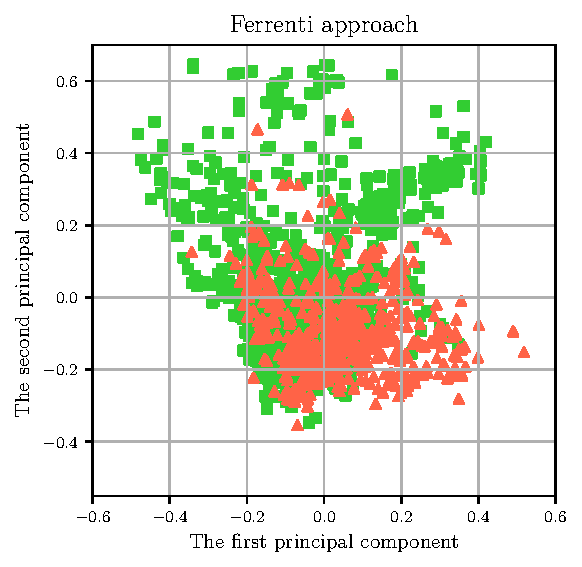
\includegraphics[width=1\textwidth]{AllFigures/01-ferrenti-approach.pdf}
    \end{subfigure}%
    \begin{subfigure}{0.35\textwidth}
        \centering
        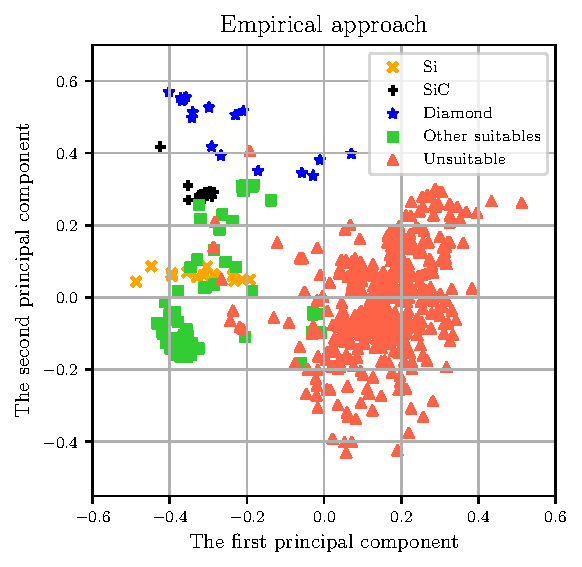
\includegraphics[width=1\textwidth]{AllFigures/03-insightful-approach.pdf}
    \end{subfigure}
    \caption{Two-dimensional scatter plots for the two different approaches. We have identified the eigenvectors corresponding to the two largest eigenvalues of the covariance-matrix, that is, the two most important principal components of the initial data from the Materials Project query. Then, we have transformed the sets of labeled data resulting from the two approaches and visualized them as scatter plots. Green squares display suitable candidates, along with the black (SiC), blue (diamond) and yellow (Si) symbols in the right panel, and red triangles represent unsuitable candidates.}
    \label{fig:2dscatterplotpca}
\end{figure}


\mrk{The Ferrenti approach and the extended Ferrenti approach share several similarities with entries that span roughly the same dimensions (not shown).} 
%For example, the entries in  Figure~\ref{fig:parallel-coordinates-approaches} span roughly the same dimensions for the Ferrenti and extended Ferrenti approaches, despite the more restricted nature of the former.  
%Moreover, the two approaches' upper limits for ionic character and covalent range are very similar in the case of candidates labeled as both suitable and unsuitable.   
The most striking difference is found for the empirical approach. \mrk{The entries labeled as suitable candidates do not exhibit any magnetization, which is also the case for the Ferrenti approach, but now the materials crystallize in both polar and non-polar space groups.} Moreover, we observe that the range of covalent radius and maximum ionic character span a substantially smaller parameter space in the case of the empirical approach than for \mrk{the former one.} 
Here, we can begin to deduce some trends, if the findings from the empirical approach are taken as guidance. In the empirical approach the polarity of the material's space group may be less important compared to the \mrk{Ferrenti approach}, while the accepted values for ionic character and covalent range appear more restricted (Fig.~\ref{fig:parallel-coordinates-approaches}). 

\mrk{To illustrate the composition of the labeled data a principal component analysis (PCA) was performed \cite{Jolliffe2002}. PCA was applied to the labeled datasets in order to reveal specific features that stand out.} In its standard  form, PCA relates the variance of the features with the eigenvalues of the covariance matrix \cite{Jolliffe2002,Murphy2012,Hastie2009}. We identify the two largest eigenvalues of the covariance matrix \cite{Hastie2009} of the complete initial dataset from the MP database, and transform the three labeled datasets according to the corresponding two eigenvectors. In essence, we reduce the dimensionality of the labeled data in order to visualize them.
The result of this procedure is displayed in the scatter plots of Fig.~\ref{fig:2dscatterplotpca}. Note that some minor differences between the three panels in Fig.~\ref{fig:2dscatterplotpca} may occur due to the process of removing the mean and scaling to unit variance. Red triangles represent unsuitable candidates while \mrk{otherwise} colored symbols (green, blue, black and yellow) represent suitable candidates. 
Due to the complexity of reducing the large amount of features down to only two, suitable and unsuitable candidates for \mrk{the Ferrenti approach} are largely overlapping. 
The logic behind categorizing materials in two classes (suitable and unsuitable) appears to not translate into a distinct separation, at least not in the representation of Fig.~\ref{fig:2dscatterplotpca} for the Ferrenti \mrk{approach}.  
Hence, using \mrk{this approach} for predicting QT material hosts could prove challenging for any model that would try to glean a clear-cut boundary between materials that are and are not suitable for QT. 
We therefore expect that the \mrk{Ferrenti approach} could need supplementary dimensions for further distinguishing between the materials in the two categories (suitable and unsuitable), or that it may prove challenging to find a generalized model based on the training sets that were defined according to the above discussion. 

In the case of the empirical approach, on the other hand, we can discern a trend where the upper left part of Fig.~\ref{fig:2dscatterplotpca} is dominated by suitable candidates (green, blue, yellow and black symbols), while the unsuitable candidates (red triangles) are similarly restricted to the lower right corner, albeit with some exceptions. 
Interestingly, we observe that different configurations of the famously quantum compatible materials of diamond (blue), silicon carbide (black) and silicon (yellow) are grouped together but each material class is separated in its own region. 
This indicates that the empirical approach may be capable of separating materials based on their underlying properties. Thus, devising a logical framework for the data mining process is likely important in order to obtain suitable datasets for training and testing of the ML methods. 

%MB Repetition, I took this out 
%After selecting and fine-tuning the entries for our labeled datasets we are now ready to apply the four ML methods discussed earlier. We split our labeled datasets into a so-called training set and a test set which is not included in the training process. This process will allow us to classify specific materials as potential candidates for quantum technology applications. 

\subsection*{Machine learning and principal component analysis}
\mrk{Four well-tested ML algorithms were applied to the labeled data} to classify specific materials as candidate systems for QT. These are logistic regression, decision trees, and the ensemble methods random forests and gradient boosting \cite{Mehta2019,Hastie2009,Murphy2012}. 
These four ML methods were applied to the labeled data sets that were optimized using each of the three approaches (Ferrenti, extended Ferrenti and empirical) outlined above, yielding twelve sets of candidates that were predicted as suitable material hosts for QT applications.  

In order to reduce the dimensionality while preserving most of the variance in the data, 
\mrk{a principal component analysis  \cite{Jolliffe2002} was performed} for each of the three approaches (Ferrenti, extended Ferrenti and empirical).
First, the eigenvalues of the covariance matrices of the three training sets are identified in order of decreasing value, resulting in three distinct PCA models (as opposed to the case of Fig.~\ref{fig:2dscatterplotpca} where all panels are based on the same model). 
Next, in the evaluation of the ML methods for the three different approaches we apply a $5\times 5$ stratified cross-validation \cite{Hastie2009} when searching for the optimal hyperparameter combinations. \mrk{Note} that all four ML methods have high evaluation metrics for the optimal hyperparameters. Further details on the evaluation of the ML methods and the results from the principal component analyses for all four \mrk{ML} methods are shown in the Supplementary Information \cite{supplementary}.  
The \mrk{data labeling approaches} define sets of labeled data of varying sizes, where the smallest is from the empirical approach. For small datasets, it is proven to be beneficial to repeat the cross-validation analysis \cite{Hastie2009}, as this is a method that allows us to measure the stability of the predictions against perturbations (i.e., few different entries) in the training data \cite{Beleites2008}.

Figure~\ref{fig:PComponents} visualizes different parameters for the most important principal components ranked in descending order by (a) the explained variance for the Ferrenti (upper panel) and empirical (lower panel) approach, and (b) the gradient boosting coefficients for the corresponding approaches. This differs from Fig.~\ref{fig:2dscatterplotpca}, where \mrk{the two most important eigenvectors for all approaches that originate from the same covariance matrix are shown}. Note also that in  Fig.~\ref{fig:2dscatterplotpca} \mrk{a PCA analysis was performed on all the data}. Here, the ML analysis is done on the labeled data for each approach. For the Ferrenti approach (Fig.~\ref{fig:PComponents}a) to reach the $95 \ \%$ accumulated explained variance, a total of $144$ principal components must be included. \mrk{In the case of the empirical approach and in contrast to the Ferrenti approach}, decision trees and random forests exhibit the best performance for just a few principal components, and experience a considerable degree of overfitting when involving more principal components. Gradient boosting 
also experiences the best performance for just a few principal components. 

\begin{figure}[t]
    \centering
    \begin{subfigure}[b]{0.45\textwidth}
        % This file was created by tikzplotlib v0.9.8.
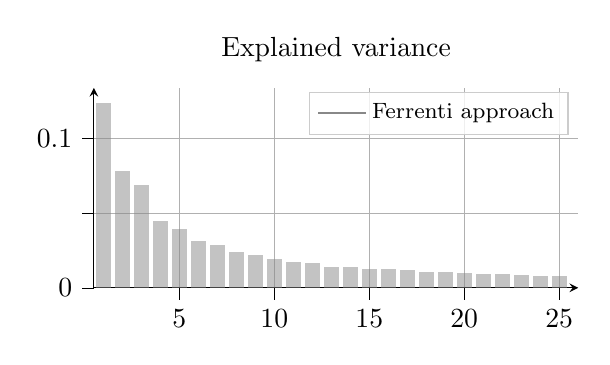
\begin{tikzpicture}

\definecolor{color0}{rgb}{0.8,0.4,0.466666666666667}

\begin{axis}[
height=1.6222438079424382in,
legend style={fill opacity=0.8, draw opacity=1, text opacity=1, draw=white!80!black},
tick align=outside,
tick pos=left,
width=3.0444876158848764in,
x grid style={white!69.0196078431373!black},
xmajorgrids,
xmin=0.5, xmax=26,
xtick style={color=black},
y grid style={white!69.0196078431373!black},
ymajorgrids,
ymin=0, ymax=0.133808014644924,
ytick style={color=black},
yticklabels={, 0, , 0.1},
title={Explained variance},
legend style={font=\footnotesize},
]
\draw[draw=none,fill=white!53.3333333333333!black,fill opacity=0.5] (axis cs:0.6,0) rectangle (axis cs:1.4,0.123808014644924);
\draw[draw=none,fill=white!53.3333333333333!black,fill opacity=0.5] (axis cs:1.6,0) rectangle (axis cs:2.4,0.0779020383908885);
\draw[draw=none,fill=white!53.3333333333333!black,fill opacity=0.5] (axis cs:2.6,0) rectangle (axis cs:3.4,0.0690715494994265);
\draw[draw=none,fill=white!53.3333333333333!black,fill opacity=0.5] (axis cs:3.6,0) rectangle (axis cs:4.4,0.0448634890553009);
\draw[draw=none,fill=white!53.3333333333333!black,fill opacity=0.5] (axis cs:4.6,0) rectangle (axis cs:5.4,0.0396017649392185);
\draw[draw=none,fill=white!53.3333333333333!black,fill opacity=0.5] (axis cs:5.6,0) rectangle (axis cs:6.4,0.0309892340254588);
\draw[draw=none,fill=white!53.3333333333333!black,fill opacity=0.5] (axis cs:6.6,0) rectangle (axis cs:7.4,0.0286471759268761);
\draw[draw=none,fill=white!53.3333333333333!black,fill opacity=0.5] (axis cs:7.6,0) rectangle (axis cs:8.4,0.0241373022722755);
\draw[draw=none,fill=white!53.3333333333333!black,fill opacity=0.5] (axis cs:8.6,0) rectangle (axis cs:9.4,0.0219387724823991);
\draw[draw=none,fill=white!53.3333333333333!black,fill opacity=0.5] (axis cs:9.6,0) rectangle (axis cs:10.4,0.0191941500093896);
\draw[draw=none,fill=white!53.3333333333333!black,fill opacity=0.5] (axis cs:10.6,0) rectangle (axis cs:11.4,0.0170987447716404);
\draw[draw=none,fill=white!53.3333333333333!black,fill opacity=0.5] (axis cs:11.6,0) rectangle (axis cs:12.4,0.0163324377943715);
\draw[draw=none,fill=white!53.3333333333333!black,fill opacity=0.5] (axis cs:12.6,0) rectangle (axis cs:13.4,0.0142479118996461);
\draw[draw=none,fill=white!53.3333333333333!black,fill opacity=0.5] (axis cs:13.6,0) rectangle (axis cs:14.4,0.0139471831901937);
\draw[draw=none,fill=white!53.3333333333333!black,fill opacity=0.5] (axis cs:14.6,0) rectangle (axis cs:15.4,0.0125561362477749);
\draw[draw=none,fill=white!53.3333333333333!black,fill opacity=0.5] (axis cs:15.6,0) rectangle (axis cs:16.4,0.0122752355665442);
\draw[draw=none,fill=white!53.3333333333333!black,fill opacity=0.5] (axis cs:16.6,0) rectangle (axis cs:17.4,0.0117377683648439);
\draw[draw=none,fill=white!53.3333333333333!black,fill opacity=0.5] (axis cs:17.6,0) rectangle (axis cs:18.4,0.0108124054147357);
\draw[draw=none,fill=white!53.3333333333333!black,fill opacity=0.5] (axis cs:18.6,0) rectangle (axis cs:19.4,0.0105912984624588);
\draw[draw=none,fill=white!53.3333333333333!black,fill opacity=0.5] (axis cs:19.6,0) rectangle (axis cs:20.4,0.00987028371434172);
\draw[draw=none,fill=white!53.3333333333333!black,fill opacity=0.5] (axis cs:20.6,0) rectangle (axis cs:21.4,0.00946157777094173);
\draw[draw=none,fill=white!53.3333333333333!black,fill opacity=0.5] (axis cs:21.6,0) rectangle (axis cs:22.4,0.00932051055389097);
\draw[draw=none,fill=white!53.3333333333333!black,fill opacity=0.5] (axis cs:22.6,0) rectangle (axis cs:23.4,0.00851928669553865);
\draw[draw=none,fill=white!53.3333333333333!black,fill opacity=0.5] (axis cs:23.6,0) rectangle (axis cs:24.4,0.00821174057436937);
\draw[draw=none,fill=white!53.3333333333333!black,fill opacity=0.5] (axis cs:24.6,0) rectangle (axis cs:25.4,0.00796122578616887);
\addlegendimage{semithick, color=white!53.3333333333333!black};
\addlegendentry{Ferrenti approach};
\end{axis}

\end{tikzpicture}

        \label{fig:01-fi-e}
    \end{subfigure}
    \begin{subfigure}[b]{0.45\textwidth}
        % This file was created by tikzplotlib v0.9.8.
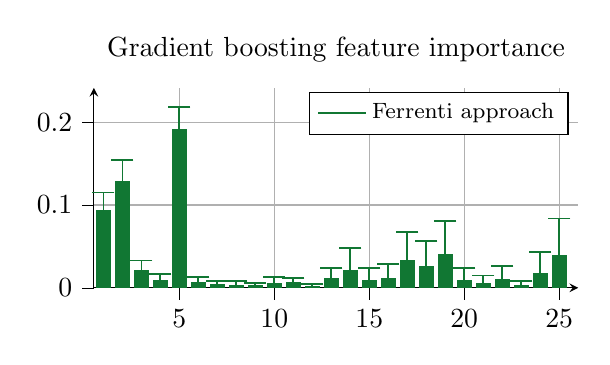
\begin{tikzpicture}

\definecolor{color0}{rgb}{0.0666666666666667,0.466666666666667,0.2}

\begin{axis}[
height=1.6222438079424382in,
tick align=outside,
tick pos=left,
width=3.0444876158848764in,
x grid style={white!69.0196078431373!black},
xmajorgrids,
xmin=0.5, xmax=26,
xtick style={color=black},
y grid style={white!69.0196078431373!black},
ymajorgrids,
ymin=0, ymax=0.241504672452706,
ytick style={color=black},
yticklabels={,0, 0.1,0.2},
title={Gradient boosting feature importance},
legend style={font=\footnotesize},
]
\draw[draw=none,fill=color0] (axis cs:0.6,0) rectangle (axis cs:1.4,0.0939219294354606);
\draw[draw=none,fill=color0] (axis cs:1.6,0) rectangle (axis cs:2.4,0.128717126999015);
\draw[draw=none,fill=color0] (axis cs:2.6,0) rectangle (axis cs:3.4,0.0213938886864563);
\draw[draw=none,fill=color0] (axis cs:3.6,0) rectangle (axis cs:4.4,0.00888144685168664);
\draw[draw=none,fill=color0] (axis cs:4.6,0) rectangle (axis cs:5.4,0.191504672452706);
\draw[draw=none,fill=color0] (axis cs:5.6,0) rectangle (axis cs:6.4,0.00724897098092836);
\draw[draw=none,fill=color0] (axis cs:6.6,0) rectangle (axis cs:7.4,0.00450287540874152);
\draw[draw=none,fill=color0] (axis cs:7.6,0) rectangle (axis cs:8.4,0.00389892865504545);
\draw[draw=none,fill=color0] (axis cs:8.6,0) rectangle (axis cs:9.4,0.00328938623970718);
\draw[draw=none,fill=color0] (axis cs:9.6,0) rectangle (axis cs:10.4,0.00607634168998537);
\draw[draw=none,fill=color0] (axis cs:10.6,0) rectangle (axis cs:11.4,0.0075927359484662);
\draw[draw=none,fill=color0] (axis cs:11.6,0) rectangle (axis cs:12.4,0.00246964434307127);
\draw[draw=none,fill=color0] (axis cs:12.6,0) rectangle (axis cs:13.4,0.0113273434472604);
\draw[draw=none,fill=color0] (axis cs:13.6,0) rectangle (axis cs:14.4,0.0215526621032538);
\draw[draw=none,fill=color0] (axis cs:14.6,0) rectangle (axis cs:15.4,0.00889067969625317);
\draw[draw=none,fill=color0] (axis cs:15.6,0) rectangle (axis cs:16.4,0.0112833024636162);
\draw[draw=none,fill=color0] (axis cs:16.6,0) rectangle (axis cs:17.4,0.0331145663678211);
\draw[draw=none,fill=color0] (axis cs:17.6,0) rectangle (axis cs:18.4,0.0265656605925389);
\draw[draw=none,fill=color0] (axis cs:18.6,0) rectangle (axis cs:19.4,0.0412663962030667);
\draw[draw=none,fill=color0] (axis cs:19.6,0) rectangle (axis cs:20.4,0.00893277229511404);
\draw[draw=none,fill=color0] (axis cs:20.6,0) rectangle (axis cs:21.4,0.00638009737027819);
\draw[draw=none,fill=color0] (axis cs:21.6,0) rectangle (axis cs:22.4,0.0110083486001703);
\draw[draw=none,fill=color0] (axis cs:22.6,0) rectangle (axis cs:23.4,0.00396903870317716);
\draw[draw=none,fill=color0] (axis cs:23.6,0) rectangle (axis cs:24.4,0.0182603050195842);
\draw[draw=none,fill=color0] (axis cs:24.6,0) rectangle (axis cs:25.4,0.0400563256690563);
\path [draw=color0, semithick]
(axis cs:1,0.0728244166732798)
--(axis cs:1,0.115019442197641);

\path [draw=color0, semithick]
(axis cs:2,0.102746647015722)
--(axis cs:2,0.154687606982308);

\path [draw=color0, semithick]
(axis cs:3,0.0096504157614985)
--(axis cs:3,0.0331373616114142);

\path [draw=color0, semithick]
(axis cs:4,0.00120429954877644)
--(axis cs:4,0.0165585941545968);

\path [draw=color0, semithick]
(axis cs:5,0.164674846558901)
--(axis cs:5,0.218334498346511);

\path [draw=color0, semithick]
(axis cs:6,0.00131865659765555)
--(axis cs:6,0.0131792853642012);

\path [draw=color0, semithick]
(axis cs:7,0.00089826602034204)
--(axis cs:7,0.008107484797141);

\path [draw=color0, semithick]
(axis cs:8,-0.000515167535189504)
--(axis cs:8,0.00831302484528041);

\path [draw=color0, semithick]
(axis cs:9,0.000577548695504199)
--(axis cs:9,0.00600122378391017);

\path [draw=color0, semithick]
(axis cs:10,-0.00123032392384619)
--(axis cs:10,0.0133830073038169);

\path [draw=color0, semithick]
(axis cs:11,0.00341822410793035)
--(axis cs:11,0.0117672477890021);

\path [draw=color0, semithick]
(axis cs:12,0.000427923119383559)
--(axis cs:12,0.00451136556675897);

\path [draw=color0, semithick]
(axis cs:13,-0.000894751232806041)
--(axis cs:13,0.0235494381273268);

\path [draw=color0, semithick]
(axis cs:14,-0.00534323462302397)
--(axis cs:14,0.0484485588295317);

\path [draw=color0, semithick]
(axis cs:15,-0.00580574316011168)
--(axis cs:15,0.023587102552618);

\path [draw=color0, semithick]
(axis cs:16,-0.0063295986999169)
--(axis cs:16,0.0288962036271493);

\path [draw=color0, semithick]
(axis cs:17,-0.000960237853350046)
--(axis cs:17,0.0671893705889922);

\path [draw=color0, semithick]
(axis cs:18,-0.00343303381845922)
--(axis cs:18,0.056564355003537);

\path [draw=color0, semithick]
(axis cs:19,0.00206699809958492)
--(axis cs:19,0.0804657943065485);

\path [draw=color0, semithick]
(axis cs:20,-0.00625580047143954)
--(axis cs:20,0.0241213450616676);

\path [draw=color0, semithick]
(axis cs:21,-0.00190515682114497)
--(axis cs:21,0.0146653515617014);

\path [draw=color0, semithick]
(axis cs:22,-0.00451438685233842)
--(axis cs:22,0.0265310840526791);

\path [draw=color0, semithick]
(axis cs:23,-0.000399848870586143)
--(axis cs:23,0.00833792627694046);

\path [draw=color0, semithick]
(axis cs:24,-0.0070765748506951)
--(axis cs:24,0.0435971848898635);

\path [draw=color0, semithick]
(axis cs:25,-0.00342720675075281)
--(axis cs:25,0.0835398580888655);
\addlegendimage{semithick, color=color0};
\addlegendentry{Ferrenti approach};
\addplot [semithick, color0, mark=-, mark size=0, mark options={solid}, only marks]
table {%
1 0.0728244166732798
2 0.102746647015722
3 0.0096504157614985
4 0.00120429954877644
5 0.164674846558901
6 0.00131865659765555
7 0.00089826602034204
8 -0.000515167535189504
9 0.000577548695504199
10 -0.00123032392384619
11 0.00341822410793035
12 0.000427923119383559
13 -0.000894751232806041
14 -0.00534323462302397
15 -0.00580574316011168
16 -0.0063295986999169
17 -0.000960237853350046
18 -0.00343303381845922
19 0.00206699809958492
20 -0.00625580047143954
21 -0.00190515682114497
22 -0.00451438685233842
23 -0.000399848870586143
24 -0.0070765748506951
25 -0.00342720675075281
};
\addplot [semithick, color0, mark=-, mark size=4, mark options={solid}, only marks]
table {%
1 0.115019442197641
2 0.154687606982308
3 0.0331373616114142
4 0.0165585941545968
5 0.218334498346511
6 0.0131792853642012
7 0.008107484797141
8 0.00831302484528041
9 0.00600122378391017
10 0.0133830073038169
11 0.0117672477890021
12 0.00451136556675897
13 0.0235494381273268
14 0.0484485588295317
15 0.023587102552618
16 0.0288962036271493
17 0.0671893705889922
18 0.056564355003537
19 0.0804657943065485
20 0.0241213450616676
21 0.0146653515617014
22 0.0265310840526791
23 0.00833792627694046
24 0.0435971848898635
25 0.0835398580888655
};
\end{axis}

\end{tikzpicture}
        \label{fig:01-fi-d}
    \end{subfigure}%
    \hfill
    \begin{subfigure}[b]{0.45\textwidth}
        % This file was created by tikzplotlib v0.9.8.
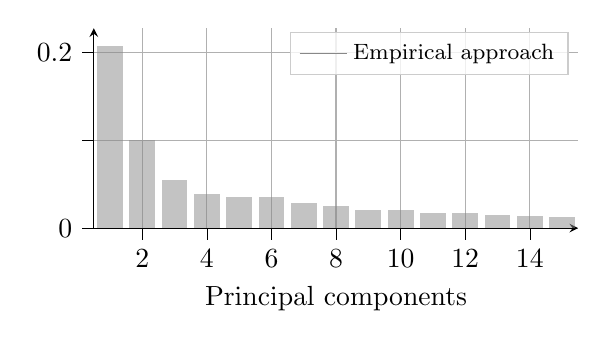
\begin{tikzpicture}

\begin{axis}[
height=1.6222438079424382in,
legend style={fill opacity=0.8, draw opacity=1, text opacity=1, draw=white!80!black},
tick align=outside,
tick pos=left,
width=3.0444876158848764in,
x grid style={white!69.0196078431373!black},
xmajorgrids,
xmin=0.5, xmax=15.5,
xlabel={Principal components},
xtick style={color=black},
y grid style={white!69.0196078431373!black},
ymajorgrids,
ymin=0, ymax=0.227659111193136,
ytick style={color=black},
yticklabels={,0,, 0.2},
legend style={font=\footnotesize}
]
\draw[draw=none,fill=white!53.3333333333333!black,fill opacity=0.5] (axis cs:0.6,0) rectangle (axis cs:1.4,0.207659111193136);
\draw[draw=none,fill=white!53.3333333333333!black,fill opacity=0.5] (axis cs:1.6,0) rectangle (axis cs:2.4,0.100931286761405);
\draw[draw=none,fill=white!53.3333333333333!black,fill opacity=0.5] (axis cs:2.6,0) rectangle (axis cs:3.4,0.0552189869141694);
\draw[draw=none,fill=white!53.3333333333333!black,fill opacity=0.5] (axis cs:3.6,0) rectangle (axis cs:4.4,0.0393144279067069);
\draw[draw=none,fill=white!53.3333333333333!black,fill opacity=0.5] (axis cs:4.6,0) rectangle (axis cs:5.4,0.0359175173728584);
\draw[draw=none,fill=white!53.3333333333333!black,fill opacity=0.5] (axis cs:5.6,0) rectangle (axis cs:6.4,0.0352100230844184);
\draw[draw=none,fill=white!53.3333333333333!black,fill opacity=0.5] (axis cs:6.6,0) rectangle (axis cs:7.4,0.0281116402524651);
\draw[draw=none,fill=white!53.3333333333333!black,fill opacity=0.5] (axis cs:7.6,0) rectangle (axis cs:8.4,0.0255858301182614);
\draw[draw=none,fill=white!53.3333333333333!black,fill opacity=0.5] (axis cs:8.6,0) rectangle (axis cs:9.4,0.020895147833239);
\draw[draw=none,fill=white!53.3333333333333!black,fill opacity=0.5] (axis cs:9.6,0) rectangle (axis cs:10.4,0.020208986578298);
\draw[draw=none,fill=white!53.3333333333333!black,fill opacity=0.5] (axis cs:10.6,0) rectangle (axis cs:11.4,0.0173851755021279);
\draw[draw=none,fill=white!53.3333333333333!black,fill opacity=0.5] (axis cs:11.6,0) rectangle (axis cs:12.4,0.0170402398481309);
\draw[draw=none,fill=white!53.3333333333333!black,fill opacity=0.5] (axis cs:12.6,0) rectangle (axis cs:13.4,0.0150421767580223);
\draw[draw=none,fill=white!53.3333333333333!black,fill opacity=0.5] (axis cs:13.6,0) rectangle (axis cs:14.4,0.0135123051552189);
\draw[draw=none,fill=white!53.3333333333333!black,fill opacity=0.5] (axis cs:14.6,0) rectangle (axis cs:15.4,0.0123812036773514);
\draw[draw=none,fill=white!53.3333333333333!black,fill opacity=0.5] (axis cs:15.6,0) rectangle (axis cs:16.4,0.0121461292946794);
\draw[draw=none,fill=white!53.3333333333333!black,fill opacity=0.5] (axis cs:16.6,0) rectangle (axis cs:17.4,0.0113049221584044);
\draw[draw=none,fill=white!53.3333333333333!black,fill opacity=0.5] (axis cs:17.6,0) rectangle (axis cs:18.4,0.0105679286164572);
\draw[draw=none,fill=white!53.3333333333333!black,fill opacity=0.5] (axis cs:18.6,0) rectangle (axis cs:19.4,0.0099240637848415);
\draw[draw=none,fill=white!53.3333333333333!black,fill opacity=0.5] (axis cs:19.6,0) rectangle (axis cs:20.4,0.00947939547970391);
\draw[draw=none,fill=white!53.3333333333333!black,fill opacity=0.5] (axis cs:20.6,0) rectangle (axis cs:21.4,0.00880748003307345);
\draw[draw=none,fill=white!53.3333333333333!black,fill opacity=0.5] (axis cs:21.6,0) rectangle (axis cs:22.4,0.00854299753930025);
\draw[draw=none,fill=white!53.3333333333333!black,fill opacity=0.5] (axis cs:22.6,0) rectangle (axis cs:23.4,0.00819923337711622);
\draw[draw=none,fill=white!53.3333333333333!black,fill opacity=0.5] (axis cs:23.6,0) rectangle (axis cs:24.4,0.00783441956089457);
\draw[draw=none,fill=white!53.3333333333333!black,fill opacity=0.5] (axis cs:24.6,0) rectangle (axis cs:25.4,0.00725436756435554);
\draw[draw=none,fill=white!53.3333333333333!black,fill opacity=0.5] (axis cs:25.6,0) rectangle (axis cs:26.4,0.00706748361834891);
\draw[draw=none,fill=white!53.3333333333333!black,fill opacity=0.5] (axis cs:26.6,0) rectangle (axis cs:27.4,0.0067946334120975);
\draw[draw=none,fill=white!53.3333333333333!black,fill opacity=0.5] (axis cs:27.6,0) rectangle (axis cs:28.4,0.00649269621923748);
\draw[draw=none,fill=white!53.3333333333333!black,fill opacity=0.5] (axis cs:28.6,0) rectangle (axis cs:29.4,0.00631012021109268);
\draw[draw=none,fill=white!53.3333333333333!black,fill opacity=0.5] (axis cs:29.6,0) rectangle (axis cs:30.4,0.0059935965924482);
\draw[draw=none,fill=white!53.3333333333333!black,fill opacity=0.5] (axis cs:30.6,0) rectangle (axis cs:31.4,0.00591276082294336);
\draw[draw=none,fill=white!53.3333333333333!black,fill opacity=0.5] (axis cs:31.6,0) rectangle (axis cs:32.4,0.00563442172532614);
\draw[draw=none,fill=white!53.3333333333333!black,fill opacity=0.5] (axis cs:32.6,0) rectangle (axis cs:33.4,0.00539612814948874);
\draw[draw=none,fill=white!53.3333333333333!black,fill opacity=0.5] (axis cs:33.6,0) rectangle (axis cs:34.4,0.00529456870611715);
\draw[draw=none,fill=white!53.3333333333333!black,fill opacity=0.5] (axis cs:34.6,0) rectangle (axis cs:35.4,0.0052012922431412);
\draw[draw=none,fill=white!53.3333333333333!black,fill opacity=0.5] (axis cs:35.6,0) rectangle (axis cs:36.4,0.00496741617032561);
\draw[draw=none,fill=white!53.3333333333333!black,fill opacity=0.5] (axis cs:36.6,0) rectangle (axis cs:37.4,0.00483584771153227);
\draw[draw=none,fill=white!53.3333333333333!black,fill opacity=0.5] (axis cs:37.6,0) rectangle (axis cs:38.4,0.00475069774706768);
\draw[draw=none,fill=white!53.3333333333333!black,fill opacity=0.5] (axis cs:38.6,0) rectangle (axis cs:39.4,0.00453755427803973);
\draw[draw=none,fill=white!53.3333333333333!black,fill opacity=0.5] (axis cs:39.6,0) rectangle (axis cs:40.4,0.00431289524873035);
\draw[draw=none,fill=white!53.3333333333333!black,fill opacity=0.5] (axis cs:40.6,0) rectangle (axis cs:41.4,0.00413291864955501);
\draw[draw=none,fill=white!53.3333333333333!black,fill opacity=0.5] (axis cs:41.6,0) rectangle (axis cs:42.4,0.00404009691245206);
\draw[draw=none,fill=white!53.3333333333333!black,fill opacity=0.5] (axis cs:42.6,0) rectangle (axis cs:43.4,0.00384707175639724);
\draw[draw=none,fill=white!53.3333333333333!black,fill opacity=0.5] (axis cs:43.6,0) rectangle (axis cs:44.4,0.00370794252319461);
\draw[draw=none,fill=white!53.3333333333333!black,fill opacity=0.5] (axis cs:44.6,0) rectangle (axis cs:45.4,0.00360347785161737);
\draw[draw=none,fill=white!53.3333333333333!black,fill opacity=0.5] (axis cs:45.6,0) rectangle (axis cs:46.4,0.00350293803678438);
\draw[draw=none,fill=white!53.3333333333333!black,fill opacity=0.5] (axis cs:46.6,0) rectangle (axis cs:47.4,0.00335377406642866);
\draw[draw=none,fill=white!53.3333333333333!black,fill opacity=0.5] (axis cs:47.6,0) rectangle (axis cs:48.4,0.00332782254644005);
\draw[draw=none,fill=white!53.3333333333333!black,fill opacity=0.5] (axis cs:48.6,0) rectangle (axis cs:49.4,0.00325065460225723);
\draw[draw=none,fill=white!53.3333333333333!black,fill opacity=0.5] (axis cs:49.6,0) rectangle (axis cs:50.4,0.00312401268859448);
\draw[draw=none,fill=white!53.3333333333333!black,fill opacity=0.5] (axis cs:50.6,0) rectangle (axis cs:51.4,0.00307409451814868);
\draw[draw=none,fill=white!53.3333333333333!black,fill opacity=0.5] (axis cs:51.6,0) rectangle (axis cs:52.4,0.00295493366839609);
\draw[draw=none,fill=white!53.3333333333333!black,fill opacity=0.5] (axis cs:52.6,0) rectangle (axis cs:53.4,0.00283452933734321);
\draw[draw=none,fill=white!53.3333333333333!black,fill opacity=0.5] (axis cs:53.6,0) rectangle (axis cs:54.4,0.00281415629292076);
\draw[draw=none,fill=white!53.3333333333333!black,fill opacity=0.5] (axis cs:54.6,0) rectangle (axis cs:55.4,0.00277164449537654);
\draw[draw=none,fill=white!53.3333333333333!black,fill opacity=0.5] (axis cs:55.6,0) rectangle (axis cs:56.4,0.0027301380386249);
\draw[draw=none,fill=white!53.3333333333333!black,fill opacity=0.5] (axis cs:56.6,0) rectangle (axis cs:57.4,0.00269085035745271);
\draw[draw=none,fill=white!53.3333333333333!black,fill opacity=0.5] (axis cs:57.6,0) rectangle (axis cs:58.4,0.00256884319342844);
\draw[draw=none,fill=white!53.3333333333333!black,fill opacity=0.5] (axis cs:58.6,0) rectangle (axis cs:59.4,0.00252762617436217);
\draw[draw=none,fill=white!53.3333333333333!black,fill opacity=0.5] (axis cs:59.6,0) rectangle (axis cs:60.4,0.00237101574205109);
\draw[draw=none,fill=white!53.3333333333333!black,fill opacity=0.5] (axis cs:60.6,0) rectangle (axis cs:61.4,0.0023429271914207);
\draw[draw=none,fill=white!53.3333333333333!black,fill opacity=0.5] (axis cs:61.6,0) rectangle (axis cs:62.4,0.00230359137012767);
\draw[draw=none,fill=white!53.3333333333333!black,fill opacity=0.5] (axis cs:62.6,0) rectangle (axis cs:63.4,0.00221364734281885);
\draw[draw=none,fill=white!53.3333333333333!black,fill opacity=0.5] (axis cs:63.6,0) rectangle (axis cs:64.4,0.0021462360088001);
\draw[draw=none,fill=white!53.3333333333333!black,fill opacity=0.5] (axis cs:64.6,0) rectangle (axis cs:65.4,0.00211833683255068);
\draw[draw=none,fill=white!53.3333333333333!black,fill opacity=0.5] (axis cs:65.6,0) rectangle (axis cs:66.4,0.00205592806762017);
\draw[draw=none,fill=white!53.3333333333333!black,fill opacity=0.5] (axis cs:66.6,0) rectangle (axis cs:67.4,0.00203631661765791);
\draw[draw=none,fill=white!53.3333333333333!black,fill opacity=0.5] (axis cs:67.6,0) rectangle (axis cs:68.4,0.00200913992503488);
\draw[draw=none,fill=white!53.3333333333333!black,fill opacity=0.5] (axis cs:68.6,0) rectangle (axis cs:69.4,0.00198860732256562);
\draw[draw=none,fill=white!53.3333333333333!black,fill opacity=0.5] (axis cs:69.6,0) rectangle (axis cs:70.4,0.00191877504746405);
\draw[draw=none,fill=white!53.3333333333333!black,fill opacity=0.5] (axis cs:70.6,0) rectangle (axis cs:71.4,0.00183983787651402);
\draw[draw=none,fill=white!53.3333333333333!black,fill opacity=0.5] (axis cs:71.6,0) rectangle (axis cs:72.4,0.00178967267072127);
\draw[draw=none,fill=white!53.3333333333333!black,fill opacity=0.5] (axis cs:72.6,0) rectangle (axis cs:73.4,0.00176113054018146);
\draw[draw=none,fill=white!53.3333333333333!black,fill opacity=0.5] (axis cs:73.6,0) rectangle (axis cs:74.4,0.00175587755437847);
\draw[draw=none,fill=white!53.3333333333333!black,fill opacity=0.5] (axis cs:74.6,0) rectangle (axis cs:75.4,0.00166568926296783);
\draw[draw=none,fill=white!53.3333333333333!black,fill opacity=0.5] (axis cs:75.6,0) rectangle (axis cs:76.4,0.00164865674220492);
\draw[draw=none,fill=white!53.3333333333333!black,fill opacity=0.5] (axis cs:76.6,0) rectangle (axis cs:77.4,0.00163963642273892);
\draw[draw=none,fill=white!53.3333333333333!black,fill opacity=0.5] (axis cs:77.6,0) rectangle (axis cs:78.4,0.00152246485297179);
\draw[draw=none,fill=white!53.3333333333333!black,fill opacity=0.5] (axis cs:78.6,0) rectangle (axis cs:79.4,0.00150671318108692);
\draw[draw=none,fill=white!53.3333333333333!black,fill opacity=0.5] (axis cs:79.6,0) rectangle (axis cs:80.4,0.00146762230969936);
\draw[draw=none,fill=white!53.3333333333333!black,fill opacity=0.5] (axis cs:80.6,0) rectangle (axis cs:81.4,0.00144254604987905);
\draw[draw=none,fill=white!53.3333333333333!black,fill opacity=0.5] (axis cs:81.6,0) rectangle (axis cs:82.4,0.00142852516970499);
\draw[draw=none,fill=white!53.3333333333333!black,fill opacity=0.5] (axis cs:82.6,0) rectangle (axis cs:83.4,0.00140797817653715);
\draw[draw=none,fill=white!53.3333333333333!black,fill opacity=0.5] (axis cs:83.6,0) rectangle (axis cs:84.4,0.00137907370730369);
\draw[draw=none,fill=white!53.3333333333333!black,fill opacity=0.5] (axis cs:84.6,0) rectangle (axis cs:85.4,0.00137189411391102);
\draw[draw=none,fill=white!53.3333333333333!black,fill opacity=0.5] (axis cs:85.6,0) rectangle (axis cs:86.4,0.00134894755604915);
\draw[draw=none,fill=white!53.3333333333333!black,fill opacity=0.5] (axis cs:86.6,0) rectangle (axis cs:87.4,0.00131887269241828);
\draw[draw=none,fill=white!53.3333333333333!black,fill opacity=0.5] (axis cs:87.6,0) rectangle (axis cs:88.4,0.00125161529911504);
\draw[draw=none,fill=white!53.3333333333333!black,fill opacity=0.5] (axis cs:88.6,0) rectangle (axis cs:89.4,0.00123038981331776);
\draw[draw=none,fill=white!53.3333333333333!black,fill opacity=0.5] (axis cs:89.6,0) rectangle (axis cs:90.4,0.00120293547721247);
\draw[draw=none,fill=white!53.3333333333333!black,fill opacity=0.5] (axis cs:90.6,0) rectangle (axis cs:91.4,0.00118929296627723);
\draw[draw=none,fill=white!53.3333333333333!black,fill opacity=0.5] (axis cs:91.6,0) rectangle (axis cs:92.4,0.00115421686183217);
\draw[draw=none,fill=white!53.3333333333333!black,fill opacity=0.5] (axis cs:92.6,0) rectangle (axis cs:93.4,0.00113288923394035);
\draw[draw=none,fill=white!53.3333333333333!black,fill opacity=0.5] (axis cs:93.6,0) rectangle (axis cs:94.4,0.00108899958168978);
\draw[draw=none,fill=white!53.3333333333333!black,fill opacity=0.5] (axis cs:94.6,0) rectangle (axis cs:95.4,0.00107268732150737);
\draw[draw=none,fill=white!53.3333333333333!black,fill opacity=0.5] (axis cs:95.6,0) rectangle (axis cs:96.4,0.00104142782755626);
\draw[draw=none,fill=white!53.3333333333333!black,fill opacity=0.5] (axis cs:96.6,0) rectangle (axis cs:97.4,0.00101906762512476);
\draw[draw=none,fill=white!53.3333333333333!black,fill opacity=0.5] (axis cs:97.6,0) rectangle (axis cs:98.4,0.00101077830297021);
\draw[draw=none,fill=white!53.3333333333333!black,fill opacity=0.5] (axis cs:98.6,0) rectangle (axis cs:99.4,0.000989640667068959);
\draw[draw=none,fill=white!53.3333333333333!black,fill opacity=0.5] (axis cs:99.6,0) rectangle (axis cs:100.4,0.000984439118691105);
\draw[draw=none,fill=white!53.3333333333333!black,fill opacity=0.5] (axis cs:100.6,0) rectangle (axis cs:101.4,0.000960734989790538);
\draw[draw=none,fill=white!53.3333333333333!black,fill opacity=0.5] (axis cs:101.6,0) rectangle (axis cs:102.4,0.000941461336335633);
\draw[draw=none,fill=white!53.3333333333333!black,fill opacity=0.5] (axis cs:102.6,0) rectangle (axis cs:103.4,0.000928355012563315);
\draw[draw=none,fill=white!53.3333333333333!black,fill opacity=0.5] (axis cs:103.6,0) rectangle (axis cs:104.4,0.000913315342059004);
\draw[draw=none,fill=white!53.3333333333333!black,fill opacity=0.5] (axis cs:104.6,0) rectangle (axis cs:105.4,0.000897708116603778);
\draw[draw=none,fill=white!53.3333333333333!black,fill opacity=0.5] (axis cs:105.6,0) rectangle (axis cs:106.4,0.000874661763686027);
\draw[draw=none,fill=white!53.3333333333333!black,fill opacity=0.5] (axis cs:106.6,0) rectangle (axis cs:107.4,0.000854349918034593);
\draw[draw=none,fill=white!53.3333333333333!black,fill opacity=0.5] (axis cs:107.6,0) rectangle (axis cs:108.4,0.000841201883286582);
\draw[draw=none,fill=white!53.3333333333333!black,fill opacity=0.5] (axis cs:108.6,0) rectangle (axis cs:109.4,0.000819094760963474);
\addlegendimage{semithick, color=white!53.3333333333333!black};
\addlegendentry{Empirical approach};
\end{axis}

\end{tikzpicture}

        \label{fig:03-fi-e}
        \subcaption{}
    \end{subfigure}
    \begin{subfigure}[b]{0.45\textwidth}
        % This file was created by tikzplotlib v0.9.8.
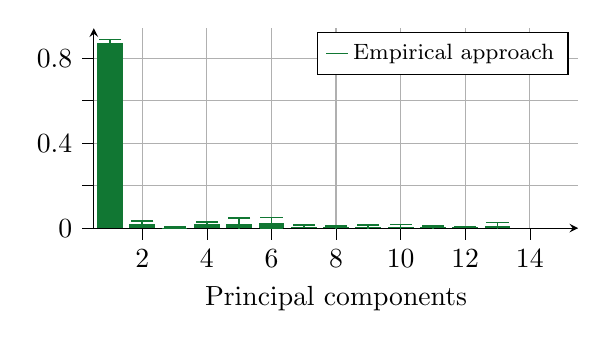
\begin{tikzpicture}

\definecolor{color0}{rgb}{0.0666666666666667,0.466666666666667,0.2}

\begin{axis}[
height=1.6222438079424382in,
tick align=outside,
tick pos=left,
width=3.0444876158848764in,
x grid style={white!69.0196078431373!black},
xmajorgrids,
xmin=0.5, xmax=15.5,
xlabel={Principal components},
xtick style={color=black},
y grid style={white!69.0196078431373!black},
ymajorgrids,
ymin=0, ymax=0.941178662009005,
yticklabels={,0,, 0.4,,0.8},
ytick style={color=black},
legend style={font=\footnotesize}
]
\draw[draw=none,fill=color0] (axis cs:0.6,0) rectangle (axis cs:1.4,0.871178662009005);
\draw[draw=none,fill=color0] (axis cs:1.6,0) rectangle (axis cs:2.4,0.0217568511840037);
\draw[draw=none,fill=color0] (axis cs:2.6,0) rectangle (axis cs:3.4,0.00253604996390695);
\draw[draw=none,fill=color0] (axis cs:3.6,0) rectangle (axis cs:4.4,0.0192708196133984);
\draw[draw=none,fill=color0] (axis cs:4.6,0) rectangle (axis cs:5.4,0.0198922275506549);
\draw[draw=none,fill=color0] (axis cs:5.6,0) rectangle (axis cs:6.4,0.0260375424696281);
\draw[draw=none,fill=color0] (axis cs:6.6,0) rectangle (axis cs:7.4,0.0063356815006726);
\draw[draw=none,fill=color0] (axis cs:7.6,0) rectangle (axis cs:8.4,0.00319869517406271);
\draw[draw=none,fill=color0] (axis cs:8.6,0) rectangle (axis cs:9.4,0.00540195176007804);
\draw[draw=none,fill=color0] (axis cs:9.6,0) rectangle (axis cs:10.4,0.00695771640251456);
\draw[draw=none,fill=color0] (axis cs:10.6,0) rectangle (axis cs:11.4,0.00312270971606427);
\draw[draw=none,fill=color0] (axis cs:11.6,0) rectangle (axis cs:12.4,0.0030932299465922);
\draw[draw=none,fill=color0] (axis cs:12.6,0) rectangle (axis cs:13.4,0.0112178627094187);
\path [draw=color0, semithick]
(axis cs:1,0.854956014167526)
--(axis cs:1,0.887401309850484);

\path [draw=color0, semithick]
(axis cs:2,0.00907965200713417)
--(axis cs:2,0.0344340503608733);

\path [draw=color0, semithick]
(axis cs:3,-0.000182654889842383)
--(axis cs:3,0.00525475481765629);

\path [draw=color0, semithick]
(axis cs:4,0.00923661909617688)
--(axis cs:4,0.0293050201306199);

\path [draw=color0, semithick]
(axis cs:5,-0.00820788248180509)
--(axis cs:5,0.0479923375831149);

\path [draw=color0, semithick]
(axis cs:6,0.00143690786973603)
--(axis cs:6,0.0506381770695201);

\path [draw=color0, semithick]
(axis cs:7,-0.00149882818592621)
--(axis cs:7,0.0141701911872714);

\path [draw=color0, semithick]
(axis cs:8,-0.00213482608794717)
--(axis cs:8,0.00853221643607259);

\path [draw=color0, semithick]
(axis cs:9,-0.00260933890414728)
--(axis cs:9,0.0134132424243034);

\path [draw=color0, semithick]
(axis cs:10,-0.0038254976017747)
--(axis cs:10,0.0177409304068038);

\path [draw=color0, semithick]
(axis cs:11,-0.0044786262895489)
--(axis cs:11,0.0107240457216774);

\path [draw=color0, semithick]
(axis cs:12,-0.000395131606741384)
--(axis cs:12,0.00658159149992578);

\path [draw=color0, semithick]
(axis cs:13,-0.00413997684116445)
--(axis cs:13,0.0265757022600018);

\addplot [semithick, color0, mark=-, mark size=4, mark options={solid}, only marks]
table {%
1 0.854956014167526
2 0.00907965200713417
3 -0.000182654889842383
4 0.00923661909617688
5 -0.00820788248180509
6 0.00143690786973603
7 -0.00149882818592621
8 -0.00213482608794717
9 -0.00260933890414728
10 -0.0038254976017747
11 -0.0044786262895489
12 -0.000395131606741384
13 -0.00413997684116445
};
\addplot [semithick, color0, mark=-, mark size=4, mark options={solid}, only marks]
table {%
1 0.887401309850484
2 0.0344340503608733
3 0.00525475481765629
4 0.0293050201306199
5 0.0479923375831149
6 0.0506381770695201
7 0.0141701911872714
8 0.00853221643607259
9 0.0134132424243034
10 0.0177409304068038
11 0.0107240457216774
12 0.00658159149992578
13 0.0265757022600018
};
\addlegendimage{semithick, color=color0};
\addlegendentry{Empirical approach};
\end{axis}

\end{tikzpicture}

        \label{fig:03-fi-d}
        \subcaption{}
    \end{subfigure}
    \caption{Visualization of different parameters for the $25$ most principal components ranked in descending order by (a) the explained variance for the Ferrenti (upper panel) and empirical (lower panel) approaches, and (b) the gradient boosting coefficients for the corresponding approaches. Note that in (a) we visualize only the results of the PCA analysis while in (b) there are results of the PCA reduced training sets using gradient boosting \cite{Hastie2009,xgboost2016}. The latter shows that for the empirical approach most of the physics is represented by a few features. The results in (b) are similar to those obtained with logistic regression, decision trees and random forests.  
    }
    \label{fig:PComponents}
\end{figure}

Figure~\ref{fig:PComponents}(b) reveals that the most important feature for the gradient boosting method in the Ferrenti approach is the fifth principal component (fifth largest eigenvalue). The trend is maintained for all four ML methods (see the Supplementary Information at \cite{supplementary}). Moreover, by selecting the highest values in this eigenvector, we find that the corresponding features originate from the DFT computed band gap of the elemental solids among the elements in the compound as calculated by the Materials Agnostic Platform for Informatics and Exploration (MagPie)~\cite{magpie}. 
The second most important principal component for the Ferrenti approach exhibits significant contributions from the covalent radius, the ionic character and the packing efficiency among the elements in the composition. 
The data originates from elemental calculations from MagPie and are aggregated as either minimum, mean, standard deviation, or maximum. 
While the first principal component encompasses the largest explained variance, it does not provide a clear and specific information on which features it represents. 

%extended Ferrenti 
\mrk{Note that the} interpretation of feature importance for the extended Ferrenti approach is substantially more challenging than in the Ferrenti approach. We find for logistic regression and decision trees that no feature is different than any other in the cross-validation, mainly due to a large variety of accuracy. However, \mrk{random} forests and gradient boosting both mark the fifth principal component as important. Similar to the Ferrenti approach, the corresponding features with the highest value for the fifth principal component originate from the DFT computed band gap of the elemental solids among the elements in the composition. 

%empirical approach 
The empirical approach differs in many aspects from the Ferrenti \mrk{approach}. 
Firstly, \mrk{the} number of principal components necessary to obtain $95 \ \%$ variance is reduced to $103$ components, which is $41$ and $56$ less than the Ferrenti and extended Ferrenti approaches, respectively. Thus, the variance of the training set is found to be described with fewer principal components, indicating a simpler model. Secondly, the first principal component is by far the most important feature for all ML methods in the empirical approach, as visualized in the lower panel of Fig.~\ref{fig:PComponents}(b) for gradient boosting. Similar conclusions are reached when using logistic regression, decisions trees and random forests as classification methods (see the Supplementary Information at \cite{supplementary}). 
The distinct importance of the first principal component partly explains why we experience a high accuracy for only a single feature. The first principal component's corresponding features is a complex combination of several material properties, but we find that it includes bond orientational parameters, coordination numbers, and the radial distribution function of a compound's crystal system. 
The standard deviation of the radial distribution function appears multiple times in the list of features and is of particular importance. 
Thirdly, the empirical approach differs in how much explained variance is retained by the first component, which is $21 \ \%$, while it is $14 \ \%$ for the Ferrenti approach. 
% and $11 \ \%$ for the extended Ferrenti approach. 
We find the difference striking considering that the approaches share the same ultimate goal, but where the training sets apparently exhibit large and significant variations. 

Intriguingly, the principal components that are deemed important by \mrk{the approaches differ substantially. The Ferrenti approach places}  particular value on the material's band gap and the ionic or covalent character of the bonding. Indeed, precisely these features were used as guidance in the data labeling process. \mrk{Thus, the ML methods seem to be perpetuate the criteria imposed in the Ferrenti approach to some extent, and return the initial assumptions on which material properties may be important for QT. The ML methods may, however, still be recognizing other patterns than those originally intended in the data selection process.} \mrk{For the empirical approach, on the other hand, the selection process was not guided in terms of specific properties.} Here, the ML methods appear to be informed by other characteristics than band gap and ionic character that are more related to symmetry and crystal structure, based on the repeated appearance of bond length, orientation and radial distribution in the first principal component. In the empirical approach, the ML methods appear to be inferring that the common trend among the materials that are known to be suitable for QT is related to more complex mechanisms in the crystal structure and bonding. 

\subsection*{Predicting Suitable Material Hosts for Quantum Technology} 
After training the ML algorithms using parts of the data labeled during the \mrk{data mining process}, the ML methods were employed on the test sets. 
The number of candidates predicted by each of the four ML methods logistic regression, decision trees, random forests and gradient boosting is visualized in the Supplementary Information at \cite{supplementary} for each of the three approaches (Ferrenti, extended Ferrenti and empirical). 
An overview of the number of predicted suitable candidates as a function of a given ML algorithm's confidence is summarized in  Table~\ref{tab:probabilites}. 

\subsubsection*{The Ferrenti approach}

From the predicted dataset of $23.623$ materials  
%the four ML methods consistently predict at least $11.000$ materials as promising candidates in the case of the Ferrenti approach. 
all four ML methods agree on a total of $6804$ suitable candidates, however, many of these materials are predicted with an incidence similar to that of a coin flip. If we were to raise the minimum confidence cut-off for a prediction to, e.g., $0.75$ instead of $0.5$, the above ML algorithms would only agree on $1784$ suitable candidates. 
We find that all four ML methods admit almost all materials with a chemical formula matching the known suitable candidates (see Table~\ref{tab:qt-materials}) that were present in the labeled data. This can allow materials with \mrk{complex structures (e.g., nanostructures or 2D materials)} to be labeled as suitable candidates. Notably, the ML methods do not maintain the band gap restriction from the training set definition, where all materials with band gaps lower than $0.5$~eV were eliminated. 
This trend is not carried over to the predicted data. Indeed, \mrk{many} entries with band gaps lower than $0.5$~eV are predicted as suitable candidates by all four ML methods employed herein 
%indicating that the cut-off value we set for the band gap ($0.5$~eV for the Ferrenti approach) is not recognized by the ML algorithms 
--- despite the principal component analysis revealing that the band gap is an important feature for the machine learning classification in the Ferrenti approach. \mrk{This indicates that the ML methods are not exactly recognizing the initial selection criteria, instead finding other patterns in the dataset.} 
On the other hand, due to the known  underestimation of band gaps by the PBE  functional, the band gaps could in reality be larger for many of the materials. 

\mrk{The ML methods predict materials as suitable that are not expected according to, e.g., Ref.~\cite{Weber2010}. Indeed, NaCl is predicted as a suitable candidate to minimum confidences of $0.83$ and $0.61$ for two different configurations, despite the strong electrostatic interactions between Na and Cl and the ionic character of their bonding. Note that NaCl was excluded from being labeled as both unsuitable and suitable in the Ferrenti approach and was therefore found in the test set. For the empirical approach, NaCl was included in the labeled data in the training set as an unsuitable candidate. }

\begin{table}[t]
    \centering 
    \caption{Overview of the number of predicted suitable candidates as a function of a given ML method's confidence when the four methods in an approach agree. A threshold value of $0.5$ represents the confidence of a coin flip while $1.0$ is a fully confident prediction.}
    \begin{tabular}{c|c|c|c}
      & $0.50$ & $0.75$ & $0.85$ \\
     \hline
     Ferrenti approach &  $6804$ & $1784$ & $258$  \\
     Extended Ferrenti approach &  $9227$ & $4735$  & $2001$  \\ 
     Empirical approach & $214$ & $66$ & $9$ \\
     \hline
     All approaches together & $47$ & $6$ & 0 \\
    \end{tabular}
    \label{tab:probabilites}
\end{table} 


%\subsubsection*{The extended Ferrenti approach}
%Next, we turn to the more liberal extended Ferrenti approach containing a $78 \ \%$ larger amount of labeled data than the Ferrenti approach. The four ML methods predict at least $13.000$ materials as suitable candidates out of $22.550$ materials in the unlabeled dataset, where they all agree on a total of $9227$ predicted suitable candidates. Comparing to the labeled data reveals that all of the unlabeled candidates that are known to be suitable (see Table~\ref{tab:qt-materials}) are, in fact, predicted as suitable candidates. However, the ML methods also predict materials as suitable that we would not expect according to, e.g., \citeauthor{Weber2010} \cite{Weber2010}. All four ML algorithms predict NaCl as a suitable candidate to confidences of $0.83$ and $0.60$ for two different configurations, despite the strong electrostatic interactions between Na and Cl and the ionic character of their bonding.  
%%Indeed, single-photon emitters with sharp and bright zero-phonon lines are uncommon in materials with a strong ionic character. 
%Furthermore, although we enforced a conservative band gap restriction of $1.5$~eV for the data labeling in the extended Ferrenti approach, we still find that all four implemented ML methods predict suitable candidates that exhibit band gaps substantially lower than $0.5$~eV.  As seen above, the ML methods applied to data labeled in the Ferrenti and extended Ferrenti approach are recognizing the band gap and bonding character as important, but the resulting predicted materials do not strictly follow the anticipated guidelines. 
 
\subsubsection*{The empirical approach}
The ML methods that were trained on the data extracted in the empirical approach predict substantially fewer candidates as compared to the \mrk{Ferrenti approach}. 
A total of $842$, $1197$, $543$ and $596$ materials are classified as suitable candidates by logistic regression, decision trees, random forests and gradient boosting, respectively. All the four ML methods agree on a total of $214$ suitable candidates to $0.5$ confidence.   
%Although this is comparable to the probability of a coin toss, the agreement of the four ML algorithms lends support to the suitability of the $214$ materials. 
Note that $51$ of these have a band gap of $0.5$~eV or smaller as reported in Materials Project \cite{Jain2013,Jain2018} from PBE-level DFT calculations. Increasing the threshold to $0.75$ or $0.85$ yields $66$ or $9$ predicted suitable candidate materials in the empirical approach, respectively (see~Table~\ref{tab:probabilites}). 

Consider the $9$ materials that were classified as suitable to a confidence of $0.85$ or higher by all four ML methods in the empirical approach; BN, CdSe (2 structures), BC$_2$N (2 structures), InAs, CuI (2 structures), and ZnCd$_3$Se$_4$. 
The nine materials (considering different crystal structures) each belong to one of the four crystal systems cubic, hexagonal, tetragonal and orthorombic. Figure~\ref{fig:crystalsystems} visualizes the four different crystal systems while Table~\ref{tab:materialproperties} lists important material properties of the relevant materials as reported in the MP database.  Interestingly, \mrk{all} nine materials appear to be four-fold coordinated, \mrk{and the first two lattice vectors ($a$ and $b$) are identical in all cases} whereas $c$ may differ.  
There appears to be a high degree of symmetry present for all materials, but \mrk{no elemental and perfectly symmetric semiconductors were found} in the list. 

\begin{figure}[t]
    \centering
    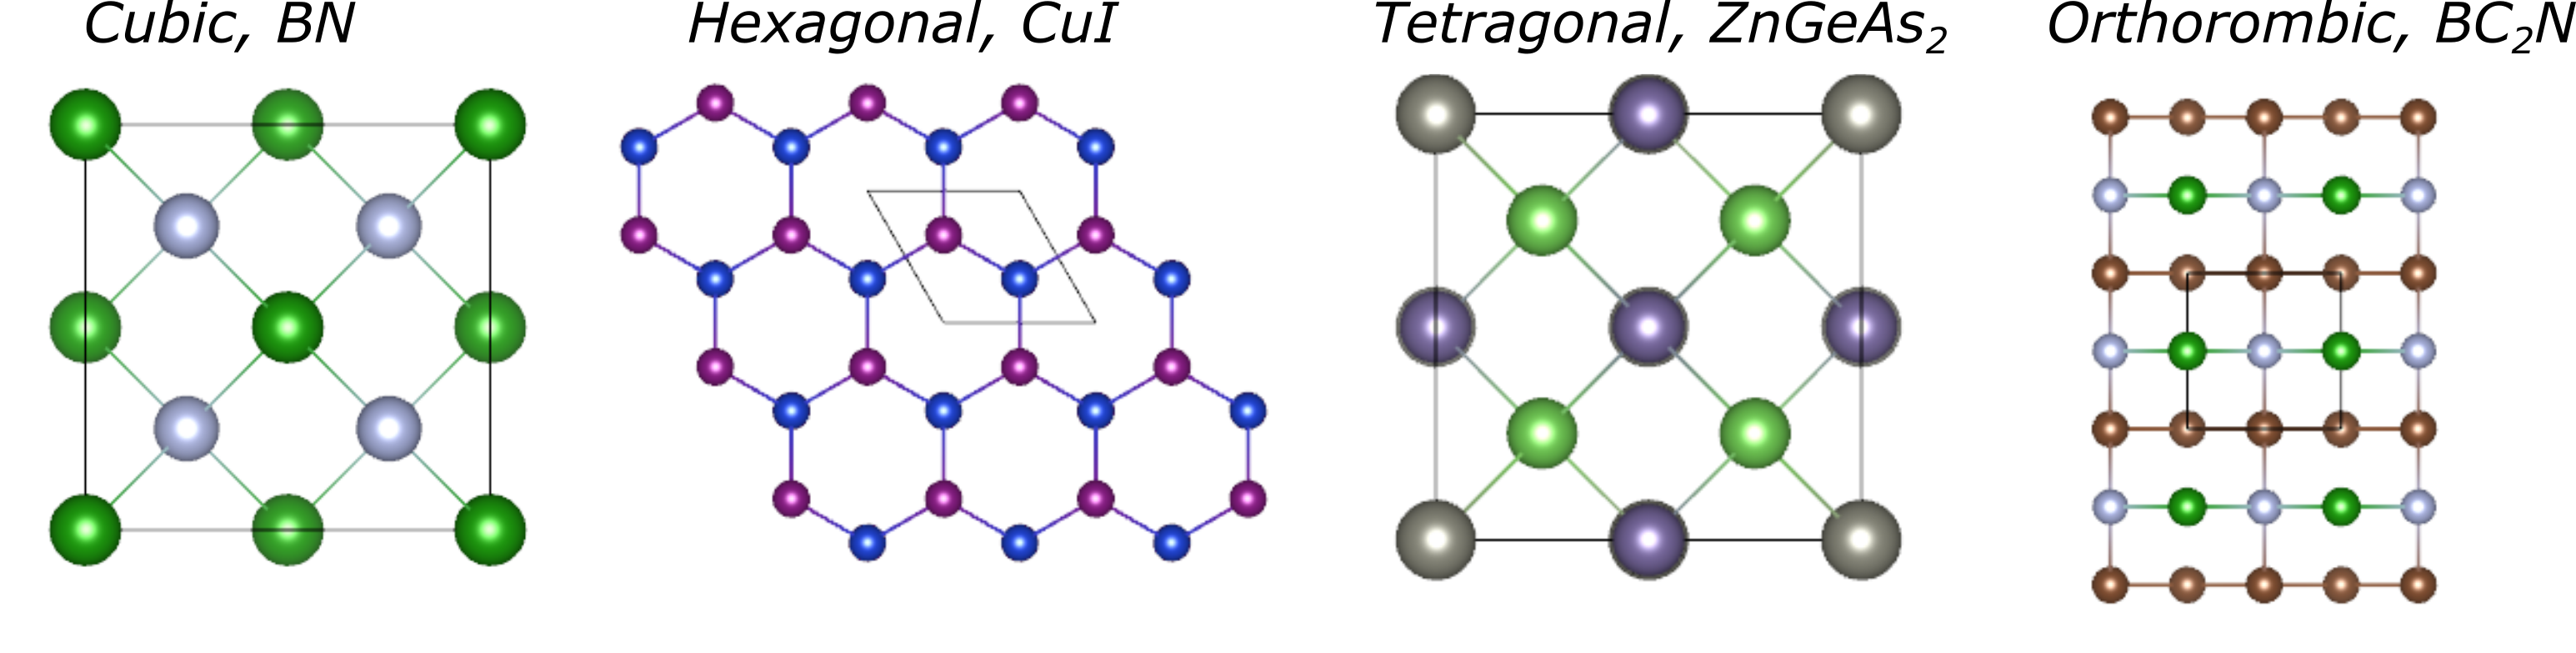
\includegraphics[width=0.85\textwidth]{AllFigures/fig6-all.png}
    \caption{Illustrations of the crystal systems that the $9$ materials predicted by the empirical approach to $0.85$ confidence, and the $6$ materials predicted by all approaches to $0.75$ confidence, may belong to. Four different symmetry categories are observed; cubic, hexagonal, tetragonal and orthorombic. The viewpoints for all materials are down along the $c$-axis.   }
    \label{fig:crystalsystems}
\end{figure}

Turning to each of the individual material predictions, the compound BN (mp-$1639$) was in fact present in the training data as a suitable candidate, and we believe this to be a partial explanation for why the ML methods recognize BN as a suitable candidate with high probability. Furthermore, two compositions of CdSe (the cubic mp-$2691$ and the hexagonal mp-$1070$) have been predicted as suitable, possibly as a consequence of the similar compound CdS being labeled as a suitable candidate in the training set. 
The two compounds of CdSe share similar properties with calculated band gaps in the MP database of $0.5$~eV and $0.6$~eV, respectively. 

In the case of BC$_2$N we find two compositions with the same chemical formula; the orthorhombically coordinated (mp-$629458$) and the tetragonally structured (mp-$1008523$) BC$_2$N. The former takes on a polar space group while the latter does not. The band gaps are listed as $1.9$~eV and $1.7$~eV, respectively, in the MP database. Both structures exhibit, as expected, a strong covalent character and have been studied for applications as nanostructures for electronic devices \cite{Gao2017}, hydrogen storage \cite{Cai2017} and superhard materials \cite{Li2017, Jiang2020}. Importantly, the diamond-like structure of BC$_3$N was recently predicted as a promising  spin qubit material host \cite{Wang2020SpinQB}. By creating a boron vacancy one can in theory obtain a defect center with similar properties to those found for the NV center in diamond. Whether this is also possible for BC$_2$N remains to be seen. \mrk{Note} that BC$_3$N was not represented in the MP database at the time of data extraction and is therefore not included in our dataset. 

The compounds InAs (cubic, mp-$20305$), CuI (cubic, mp-$22895$ and hexagonal, mp-$569346$) and ZnCd$_3$Se$_4$ (cubic, mp-$1078597$) are listed in the MP database with band gaps of $0.3$, $1.2$, $1.2$ and $1.7$~eV, respectively. 
To the best of our knowledge, ZnCd$_3$Se$_4$ has yet to be synthesized, while self-assembled InAs quantum dots are  exciting possible materials to use in quantum technology \cite{Liu2018}. 
CuI has recently been synthesized as single-crystal epitaxial films and was shown to exhibit remarkable optoelectronic properties \cite{Ahn2020}. Interestingly, the material exhibits a large ionic character with more similarities to some of the oxide compounds in the dataset than, e.g., the materials that are more covalent in character like Si, SiC and  diamond.  
The prediction of CuI in two configurations indicates that ionic character alone is not an obstacle for a material to be quantum compatible. It is unknown at this time whether any potentially favorable properties of CuI would originate from deep level defects or  nanostructuring (e.g., quantum dots). NaCl was not predicted as suitable for QT in the empirical approach\mrk{, in contrast to the Ferrenti (and extended Ferenti) approach}. 
%This underlines that an empirical approach, based on experimental data, may be more suitable for predicting materials for a certain applications and understanding the underlying mechanisms than the assumption-based methodology.}

Out of the nine predicted materials (threshold of $0.85$) we note that both instances of CuI are stated in the MP database to decompose into trigonal CuI, which was not present in our predictions. Hexagonal CdSe decomposes into cubic CdSe (in the list of $9$), the cubic BN decomposes to hexagonal BN (mp-$984$, not in the predictions), and ZnCd$_3$Se$_4$ decomposes to ZnSe $+$ CdSe (in the list). Finally, both compounds of the BC$_2$N structure are listed to decompose into hexagonal BN $+$ C. 
However, synthesis may still be possible depending on the growth conditions. 

Lowering the cut-off requirement from $0.85$ to $0.75$ for all ML methods results in $66$ candidate materials for the empirical approach.  
The full list of these $66$ candidates is displayed in the Supplementary Information at \cite{supplementary}. 
In addition to the nine materials discussed above and some elemental and binary semiconductors, the list of $66$ predicted suitable candidates now also includes ternary compounds of the formula ABC$_2$. For the ABC$_2$ structures, the elements Ga, Cd, In and Zn can occupy the A-site, Cu, Sn, Ag and Ge take the B-site, while S, Se, Te, P or As may reside at the C site. Most of the predicted compounds include at least one toxic element with one exception: ZnGeP$_2$ (mp-$4524$) in a chalcopyrite-like tetragonal crystal structure with an indirect band gap of $1.2$~eV \cite{Zhang2015} as reported in the MP database. In comparison, the experimentally reported band gap is somewhat larger at $2.0$~eV \cite{Xing1989}. 
ZnGeP$_2$ crystallizes in a non-polar space group, possesses no magnetic moment, exhibits strongly covalent bonds, and has been reported as an excellent mid-IR transparent crystal material that is suitable for nonlinear optical applications \cite{Zhang2015}. Importantly, it is possible to integrate sources of photon quantum states based on nonlinear optics with ZnGeP$_2$ \cite{Caspani2017}. 
\mrk{ZnGeP$_2$ is therefore identified} as an eligible candidate material for QT, but it remains to be seen whether the candidate can facilitate, e.g., the isolated deep energy levels often associated with defects exhibiting quantum compatible properties, or instead be a candidate for nanostructure based QT.  

\begin{table}[t]
    \centering 
    \caption{Overview of material properties as listed in the MP database for the $9$ materials predicted by the empirical approach ($>0.85$) and the $6$ materials predicted by all approaches ($>0.75$). Compounds marked by an asterisk are predicted to be unstable to transformation into other phases in the MP database. }
    \begin{tabular}{c|c c c c c c c }
      & Material & Crystal structure & MP code & Density (g/cm$^3$) & Band gap (eV) & a, b, c (\AA) & $\alpha,\beta,\gamma$ ($^\circ$) \\
    \hline 
    Empirical & CdSe & Hexagonal & mp-$1070$ & $5.3$ & $0.6$ & $4.4,4.4,7.2$ & $90,90,120$ \\
    approach  & CuI & Hexagonal & mp-$569346$ & $5.8$ & $1.2$ & $4.3,4.3,7.0$ & $90,90,120$ \\ 
    to $0.85$  & CuI & Cubic & mp-$22895$ & $5.8$ & $1.2$ & $4.3,4.3,4.3$ & $60,60,60$  \\ 
    confidence & CdSe & Cubic & mp-$2691$ & $5.3$ & $0.5$ & $4.4,4.4,4.4$ & $60,60,60$  \\
     & BN & Cubic & mp-$1639$ & $3.5$ & $4.6$ & $2.6,2.6,2.6$ & $60,60,60$  \\
     & InAs & Cubic & mp-$20305$ & $5.3$ & $0.3$ & $4.4,4.4,4.4$ & $60,60,60$ \\
     & ZnCd$_3$Se$_4$ & Cubic & mp-$1078597$ & $5.3$ & $1.7$ & $6.1,6.1,6.1$ & $90,90,90$ \\
     & BC$_2$N & Tetragonal & mp-$1008523$ & $3.3$ & $1.6$ & $2.6,2.6,3.7$ & $90,90,90$ \\
     & BC$_2$N & Orthorombic & mp-$629458$ & $3.4$ & $1.8$ & $2.5,2.6,3.6$ & $90,90,90$ \\
    \hline 
    All & CdSnP$_2$ & Tetragonal & mp-$5213$ & $4.6$ & $0.7$ & $7.2,7.2,7.2$ & $131.1,131.1,71.7$ \\
    approaches & GeSe & Cubic & mp-$10759$ & $5.5$ & $0.4$ & $4.0,4.0,4.0$ & $60,60,60$ \\
    to $0.75$  & InP & Cubic & mp-$20351$ & $4.6$ & $0.5$ & $4.2,4.2,4.2$ &  $60,60,60$\\ 
    confidence & InP & Hexagonal & mp-$966800$ & $4.6$ & $0.5$ & $4.2,4.2,6.9$ & $90,90,120$ \\ 
     & SiSn & Cubic & mp-$1009813$ & $4.4$ & $0.4$ & $4.3,4.3,4.3$ & $60,60,60$ \\
     & ZnGeAs$_2$ & Tetragonal & mp-$4008$ & $5.2$ & $0.6$ & $7.0,7.0,7.0$ & $131.4,131.4,71.2$ \\
    \end{tabular}
    \label{tab:materialproperties}
\end{table}

Among the $66$ materials that all ML methods in the empirical approach agreed on to a $0.75$ confidence level, we also emphasize the presence of interesting materials like Ge (in three configurations mp-$137$, mp-$1067619$ and mp-$1198022$), GeC, BP and InP. The element Ge in the cubic structure (mp-$1198022$) shares many properties with Si and C in addition to the periodic column number. 
Germanium has the highest hole mobility of all semiconductors at room temperature, and is therefore considered a key material for the process of extending the chip performance in classical computers beyond the limits imposed by miniaturization \cite{Scappucci2020}. Furthermore, like SiC, device design based on Ge can take advantage of the mature large-scale fabrication of silicon due to the material's comparable properties.  
Similar considerations could be made for the case of GeC. 
Data from the MP database suggests that the cubic compound GeC (mp-$1002164$) is a covalently bonded semiconductor having a band gap of $1.8$~eV. 
Consequently, with SiC being widely known as a highly suitable host material for QT compatible defects, we encourage further research on GeC due to its similarities with SiC. 
Next, the compound BP (mp-$1479$ and mp-$1008559$) is present in \mrk{the} predictions in both the cubic and hexagonal structures, with indirect band gaps calculated at $1.5$~eV and $1.1$~eV, respectively. Both configurations of BP are nonmagnetic, non-toxic and BP has been synthesized with a potential for large-scale production \cite{MukhanovVladimirA2016Umso}. 
Lastly, InP (mp-$966800$) was also predicted as a suitable candidate to $0.75$ confidence. The compound inhabits the hexagonal structure with corner-sharing InP$_4$ tetrahedra. InP is reported in the Materials Project to have a direct band gap of $0.5$~eV and is considered as one of the most promising candidates to compete with Cd- or Pb- based QDs for, e.g., display and lighting applications  \cite{Zhang2020a, Won2019}. 
\mrk{The possibility of using InP-based quantum dots for QT applications should be considered.}  

\mrk{All} ML methods in the empirical approach agree on several oxides being potential candidates when the prediction cut-off is set low enough (but still above $0.5$). \mrk{However, almost} all the oxide compounds fall between the decision boundary defining suitable and unsuitable candidates, and none are present in the list containing the $66$ suitable candidates using a $0.75$ threshold. Due to the labeling of ZnO as a suitable candidate in the training set, we believe that the boundary was shifted sufficiently to admit several oxides as suitable candidates. Removing ZnO from the training set for the empirical approach might result in fewer or even no oxide compounds being predicted above a suitability limit of $0.5$ and could be an interesting future pathway for investigation. 

Comparing to the work of \citeauthor{Ferrenti2020} \cite{Ferrenti2020}, they suggest a list of $541$ viable hosts after the data mining procedure.  
Among these, \mrk{only a single material is present in the list of $66$ candidates predicted by the four ML methods} in the empirical approach: the nontoxic compound MgSe (mp-$10760$) which crystallizes in the rock-salt structure, is expected to have a $2.0$~eV band gap and decomposes to a similar MgSe configuration. 
%The band gap of MgSe is listed as $2.0$~eV in the MP database with the experimental value being reported at $2.45$~eV (optical band gap) \cite{Ubale2014}. 
MgSe is notable for its available spin-zero isotopes in accordance with the criteria set by \citeauthor{Weber2010} \cite{Weber2010} and \citeauthor{Ferrenti2020} \cite{Ferrenti2020}. We note that these properties may favor defects acting as spin centers with qubit potential and MgSe is thus identified as an interesting host material in this regard.   

%\subsubsection*{Comparing the approaches}
\subsubsection*{Overlapping predictions between the approaches}

%\section*{\mrk{Discussion}}
%Comparing the three approaches Ferrenti, extended Ferrenti and empirical (see also Table~\ref{tab:probabilites}), we observe that the extended Ferrenti approach is the least restricted also for the predicted materials and admits the largest number of entries regardless of the confidence threshold. 
%The Ferrenti approach also predicts a large amount of materials as suitable compared to the empirical approach, but the resulting data are otherwise not very different from the extended version. The empirical approach, on the other hand, predicts fewer suitable candidates that are possible to examine  manually. 
\mrk{The amount of materials predicted by the empirical approach is restricted enough to enable close scrutiny of the various suggested candidates. The same cannot be said for the Ferrenti (and extended Ferrenti) approach, however, as seen from Table~\ref{tab:probabilites}.} Manual verification through a literature survey will often not be possible\mrk{,} and perfecting automatic data mining and analysis is therefore an important goal of material informatics \cite{rickman2019}. 

Despite notable differences, as mentioned above, there is \mrk{some overlap of predicted materials between the approaches}. 
%We find that $119$ of the $214$ candidates predicted as suitable by the empirical approach (threshold at $0.5$) were also selected by all ML methods in the extended Ferrenti approach. Similarly, $78$ of the $214$ materials are also predicted as suitable by all ML methods in the Ferrenti approach. 
All approaches \mrk{(including the extended Ferrenti approach) and their corresponding ML methods agree on a total of $47$ potential candidates to $0.5$ confidence 
%where $8$ are elementary (unary), $29$ binary, and $10$ tertiary 
(see the Supplementary Information at \cite{supplementary} for the full list).} 
Several interesting materials that were also discussed above for the predictions by the empirical approach are present among these $47$, including BP, CdSe, GeC, InP and Ge. However, certain materials that cannot be classified as semiconductors \mrk{are also included}, such as P, I, N$_2$ and H$_2$. We note that none of these were included by the empirical approach when the threshold was set to $0.75$ or above. 

Importantly, there are $6$ materials that all approaches (Ferrenti, extended Ferrenti and empirical) and ML methods agree on above a $0.75$ threshold. These are ZnGeAs$_2$ (tetragonal mp-$4008$), CdSnP$_2$ (tetragonal mp-$5213$), GeSe (cubic mp-$10759$), InP (cubic mp-$20351$), InP (hexagonal mp-$966800$) and SiSn (cubic mp-$1009813$). Here, we can distinguish three groupings in crystal structure: cubic, hexagonal and tetragonal (illustrated in Fig.~\ref{fig:crystalsystems}). The relevant material properties are summarized in the lower part of Table~\ref{tab:materialproperties}, 
%Note that hexagonal InP is listed in the MP database as decomposing into cubic InP while SiSn is stated to decompose into Si $+$ Sn. 
\mrk{with comparable trends to those for the $9$ materials predicted by the empirical approach in terms of, e.g., crystal structure. The six-fold coordination of GeSe is an outlier as compared to the four-fold coordination of the other materials. }
%We can deduce a series of similar trends as for the $9$ materials from the empirical approach --- e.g., the same space groups are manifesting, we find only binary or tertiary compounds, and $a=b$ for all materials while $c$ is different for hexagonal InP. 
%However, consistent four-fold coordination and the bond angle trends  observed for the first $9$ materials are not maintained as GeSe is six-fold coordinated. 
We highlight these six compounds, along with the nine predicted by the empirical approach to $0.85$ confidence, as particularly interesting for future in-depth theoretical and experimental studies. 

%histograms 
\begin{figure}[ht]
    \begin{subfigure}[b]{1\textwidth}
    \centering
    % This file was created by tikzplotlib v0.9.8.
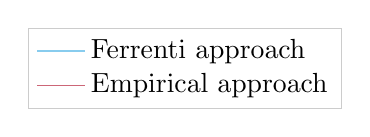
\begin{tikzpicture}

\definecolor{color0}{rgb}{0.866666666666667,0.8,0.466666666666667}
\definecolor{color1}{rgb}{0.533333333333333,0.8,0.933333333333333}
\definecolor{color3}{rgb}{0.8,0.4,0.466666666666667}
\begin{axis}[%
 hide axis,
 xmin=0,
 xmax=1,
 ymin=0,
 ymax=1,
 legend columns=1,
 legend cell align={left},
 legend style={
   fill opacity=1,
   draw opacity=1,
   text opacity=1,
   align=center,
   anchor=north,
   draw=white!80!black
 },
 ]
 \addlegendimage{semithick, color1}
 \addlegendentry{Ferrenti approach};
 \addlegendimage{semithick, color3}
 \addlegendentry{Empirical approach};
 \end{axis}

\end{tikzpicture}

  \end{subfigure}
  \par\bigskip
\begin{subfigure}[b]{0.45\textwidth}
    % This file was created with tikzplotlib v0.9.16.
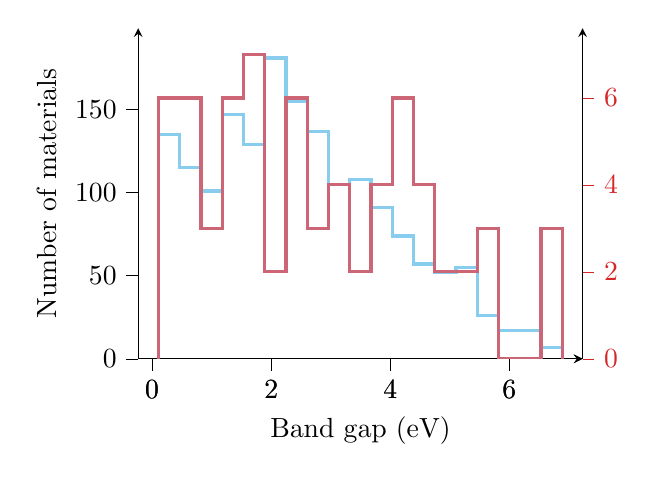
\begin{tikzpicture}

\definecolor{color0}{rgb}{0.866666666666667,0.8,0.466666666666667}
\definecolor{color1}{rgb}{0.533333333333333,0.8,0.933333333333333}
\definecolor{color2}{rgb}{0.83921568627451,0.152941176470588,0.156862745098039}
\definecolor{color3}{rgb}{0.8,0.4,0.466666666666667}

\begin{axis}[
height=2.275590092707901in,
legend cell align={left},
legend style={fill opacity=0.8, draw opacity=1, text opacity=1, draw=white!80!black, font=\footnotesize},
tick align=outside,
tick pos=left,
title={},
width=2.8444876158848764in,
x grid style={white!69.0196078431373!black},
xlabel={Band gap (eV)},
xmin=-0.234255, xmax=7.229355,
xtick style={color=black},
y grid style={white!69.0196078431373!black},
ylabel={Number of materials},
ymin=0, ymax=199.0,
ytick style={color=black}
]
\path [draw=color1, very thick]
(axis cs:0.105,0)
--(axis cs:0.105,135)
--(axis cs:0.462110526315789,135)
--(axis cs:0.462110526315789,115)
--(axis cs:0.819221052631579,115)
--(axis cs:0.819221052631579,101)
--(axis cs:1.17633157894737,101)
--(axis cs:1.17633157894737,147)
--(axis cs:1.53344210526316,147)
--(axis cs:1.53344210526316,129)
--(axis cs:1.89055263157895,129)
--(axis cs:1.89055263157895,181)
--(axis cs:2.24766315789474,181)
--(axis cs:2.24766315789474,155)
--(axis cs:2.60477368421053,155)
--(axis cs:2.60477368421053,137)
--(axis cs:2.96188421052632,137)
--(axis cs:2.96188421052632,105)
--(axis cs:3.31899473684211,105)
--(axis cs:3.31899473684211,108)
--(axis cs:3.67610526315789,108)
--(axis cs:3.67610526315789,91)
--(axis cs:4.03321578947368,91)
--(axis cs:4.03321578947368,74)
--(axis cs:4.39032631578947,74)
--(axis cs:4.39032631578947,57)
--(axis cs:4.74743684210526,57)
--(axis cs:4.74743684210526,52)
--(axis cs:5.10454736842105,52)
--(axis cs:5.10454736842105,55)
--(axis cs:5.46165789473684,55)
--(axis cs:5.46165789473684,26)
--(axis cs:5.81876842105263,26)
--(axis cs:5.81876842105263,17)
--(axis cs:6.17587894736842,17)
--(axis cs:6.17587894736842,17)
--(axis cs:6.53298947368421,17)
--(axis cs:6.53298947368421,7)
--(axis cs:6.8901,7)
--(axis cs:6.8901,0);

\end{axis}

\begin{axis}[
axis y line=right,
height=2.275590092707901in,
tick align=outside,
width=2.8444876158848764in,
x grid style={white!69.0196078431373!black},
xmin=-0.234255, xmax=7.229355,
xtick pos=left,
xtick style={color=black},
y grid style={white!69.0196078431373!black},
ymin=0, ymax=7.6,
ytick pos=right,
ytick style={color=color2},
yticklabel style={anchor=west, color=color2}
]
\path [draw=color3, very thick]
(axis cs:0.105,0)
--(axis cs:0.105,6)
--(axis cs:0.462110526315789,6)
--(axis cs:0.462110526315789,6)
--(axis cs:0.819221052631579,6)
--(axis cs:0.819221052631579,3)
--(axis cs:1.17633157894737,3)
--(axis cs:1.17633157894737,6)
--(axis cs:1.53344210526316,6)
--(axis cs:1.53344210526316,7)
--(axis cs:1.89055263157895,7)
--(axis cs:1.89055263157895,2)
--(axis cs:2.24766315789474,2)
--(axis cs:2.24766315789474,6)
--(axis cs:2.60477368421053,6)
--(axis cs:2.60477368421053,3)
--(axis cs:2.96188421052632,3)
--(axis cs:2.96188421052632,4)
--(axis cs:3.31899473684211,4)
--(axis cs:3.31899473684211,2)
--(axis cs:3.67610526315789,2)
--(axis cs:3.67610526315789,4)
--(axis cs:4.03321578947368,4)
--(axis cs:4.03321578947368,6)
--(axis cs:4.39032631578947,6)
--(axis cs:4.39032631578947,4)
--(axis cs:4.74743684210526,4)
--(axis cs:4.74743684210526,2)
--(axis cs:5.10454736842105,2)
--(axis cs:5.10454736842105,2)
--(axis cs:5.46165789473684,2)
--(axis cs:5.46165789473684,3)
--(axis cs:5.81876842105263,3)
--(axis cs:5.81876842105263,0)
--(axis cs:6.17587894736842,0)
--(axis cs:6.17587894736842,0)
--(axis cs:6.53298947368421,0)
--(axis cs:6.53298947368421,3)
--(axis cs:6.8901,3)
--(axis cs:6.8901,0);
\end{axis}

\end{tikzpicture}

    \subcaption{}
\end{subfigure}
\begin{subfigure}[b]{0.45\textwidth}
    % This file was created with tikzplotlib v0.9.16.
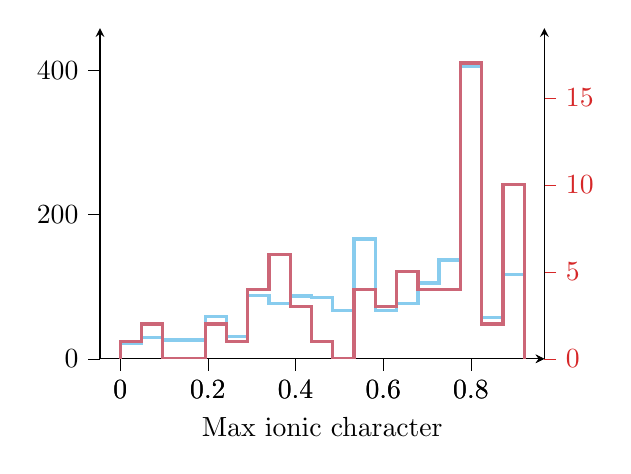
\begin{tikzpicture}

\definecolor{color0}{rgb}{0.866666666666667,0.8,0.466666666666667}
\definecolor{color1}{rgb}{0.533333333333333,0.8,0.933333333333333}
\definecolor{color2}{rgb}{0.83921568627451,0.152941176470588,0.156862745098039}
\definecolor{color3}{rgb}{0.8,0.4,0.466666666666667}

\begin{axis}[
height=2.275590092707901in,
legend cell align={left},
legend style={fill opacity=0.8, draw opacity=1, text opacity=1, draw=white!80!black},
tick align=outside,
tick pos=left,
title={},
width=2.8444876158848764in,
x grid style={white!69.0196078431373!black},
xlabel={Max ionic character},
xmin=-0.0460725199741125, xmax=0.967522919456363,
xtick style={color=black},
y grid style={white!69.0196078431373!black},
ylabel={},
ymin=0, ymax=458.35,
ytick style={color=black}
]
\path [draw=color1, very thick]
(axis cs:0,0)
--(axis cs:0,21)
--(axis cs:0.0484973894464342,21)
--(axis cs:0.0484973894464342,30)
--(axis cs:0.0969947788928685,30)
--(axis cs:0.0969947788928685,26)
--(axis cs:0.145492168339303,26)
--(axis cs:0.145492168339303,26)
--(axis cs:0.193989557785737,26)
--(axis cs:0.193989557785737,59)
--(axis cs:0.242486947232171,59)
--(axis cs:0.242486947232171,31)
--(axis cs:0.290984336678605,31)
--(axis cs:0.290984336678605,88)
--(axis cs:0.33948172612504,88)
--(axis cs:0.33948172612504,77)
--(axis cs:0.387979115571474,77)
--(axis cs:0.387979115571474,87)
--(axis cs:0.436476505017908,87)
--(axis cs:0.436476505017908,85)
--(axis cs:0.484973894464342,85)
--(axis cs:0.484973894464342,67)
--(axis cs:0.533471283910777,67)
--(axis cs:0.533471283910777,166)
--(axis cs:0.581968673357211,166)
--(axis cs:0.581968673357211,67)
--(axis cs:0.630466062803645,67)
--(axis cs:0.630466062803645,77)
--(axis cs:0.678963452250079,77)
--(axis cs:0.678963452250079,105)
--(axis cs:0.727460841696513,105)
--(axis cs:0.727460841696513,137)
--(axis cs:0.775958231142948,137)
--(axis cs:0.775958231142948,406)
--(axis cs:0.824455620589382,406)
--(axis cs:0.824455620589382,57)
--(axis cs:0.872953010035816,57)
--(axis cs:0.872953010035816,117)
--(axis cs:0.92145039948225,117)
--(axis cs:0.92145039948225,0);

\end{axis}

\begin{axis}[
axis y line=right,
height=2.275590092707901in,
tick align=outside,
width=2.8444876158848764in,
x grid style={white!69.0196078431373!black},
xmin=-0.0460725199741125, xmax=0.967522919456363,
xtick pos=left,
xtick style={color=black},
y grid style={white!69.0196078431373!black},
ymin=0, ymax=19.0,
ytick pos=right,
ytick style={color=color2},
yticklabel style={anchor=west, color=color2}
]
\path [draw=color3, very thick]
(axis cs:0,0)
--(axis cs:0,1)
--(axis cs:0.0484973894464342,1)
--(axis cs:0.0484973894464342,2)
--(axis cs:0.0969947788928685,2)
--(axis cs:0.0969947788928685,0)
--(axis cs:0.145492168339303,0)
--(axis cs:0.145492168339303,0)
--(axis cs:0.193989557785737,0)
--(axis cs:0.193989557785737,2)
--(axis cs:0.242486947232171,2)
--(axis cs:0.242486947232171,1)
--(axis cs:0.290984336678605,1)
--(axis cs:0.290984336678605,4)
--(axis cs:0.33948172612504,4)
--(axis cs:0.33948172612504,6)
--(axis cs:0.387979115571474,6)
--(axis cs:0.387979115571474,3)
--(axis cs:0.436476505017908,3)
--(axis cs:0.436476505017908,1)
--(axis cs:0.484973894464342,1)
--(axis cs:0.484973894464342,0)
--(axis cs:0.533471283910777,0)
--(axis cs:0.533471283910777,4)
--(axis cs:0.581968673357211,4)
--(axis cs:0.581968673357211,3)
--(axis cs:0.630466062803645,3)
--(axis cs:0.630466062803645,5)
--(axis cs:0.678963452250079,5)
--(axis cs:0.678963452250079,4)
--(axis cs:0.727460841696513,4)
--(axis cs:0.727460841696513,4)
--(axis cs:0.775958231142948,4)
--(axis cs:0.775958231142948,17)
--(axis cs:0.824455620589382,17)
--(axis cs:0.824455620589382,2)
--(axis cs:0.872953010035816,2)
--(axis cs:0.872953010035816,10)
--(axis cs:0.92145039948225,10)
--(axis cs:0.92145039948225,0);
\end{axis}

\end{tikzpicture}

    \subcaption{}
\end{subfigure}%

\begin{subfigure}[b]{0.45\textwidth}
    % This file was created with tikzplotlib v0.9.16.
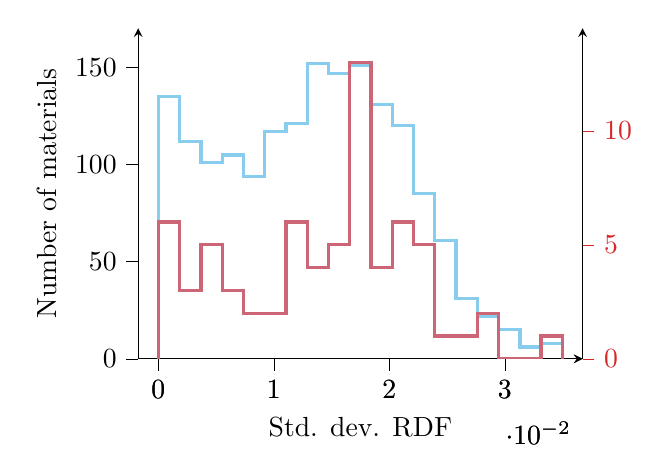
\begin{tikzpicture}

\definecolor{color0}{rgb}{0.866666666666667,0.8,0.466666666666667}
\definecolor{color1}{rgb}{0.533333333333333,0.8,0.933333333333333}
\definecolor{color2}{rgb}{0.83921568627451,0.152941176470588,0.156862745098039}
\definecolor{color3}{rgb}{0.8,0.4,0.466666666666667}

\begin{axis}[
height=2.275590092707901in,
legend cell align={left},
legend style={fill opacity=0.8, draw opacity=1, text opacity=1, draw=white!80!black},
tick align=outside,
tick pos=left,
title={},
width=2.8444876158848764in,
x grid style={white!69.0196078431373!black},
xlabel={Std. dev. RDF},
xmin=-0.00174896633573773, xmax=0.0367282930504924,
xtick style={color=black},
y grid style={white!69.0196078431373!black},
ylabel={Number of materials},
ymin=0, ymax=170.2,
ytick style={color=black}
]

\path [draw=color1, very thick]
(axis cs:0,0)
--(axis cs:0,135)
--(axis cs:0.0018410171955134,135)
--(axis cs:0.0018410171955134,112)
--(axis cs:0.00368203439102681,112)
--(axis cs:0.00368203439102681,101)
--(axis cs:0.00552305158654021,101)
--(axis cs:0.00552305158654021,105)
--(axis cs:0.00736406878205362,105)
--(axis cs:0.00736406878205362,94)
--(axis cs:0.00920508597756702,94)
--(axis cs:0.00920508597756702,117)
--(axis cs:0.0110461031730804,117)
--(axis cs:0.0110461031730804,121)
--(axis cs:0.0128871203685938,121)
--(axis cs:0.0128871203685938,152)
--(axis cs:0.0147281375641072,152)
--(axis cs:0.0147281375641072,147)
--(axis cs:0.0165691547596206,147)
--(axis cs:0.0165691547596206,151)
--(axis cs:0.018410171955134,151)
--(axis cs:0.018410171955134,131)
--(axis cs:0.0202511891506474,131)
--(axis cs:0.0202511891506474,120)
--(axis cs:0.0220922063461609,120)
--(axis cs:0.0220922063461609,85)
--(axis cs:0.0239332235416743,85)
--(axis cs:0.0239332235416743,61)
--(axis cs:0.0257742407371877,61)
--(axis cs:0.0257742407371877,31)
--(axis cs:0.0276152579327011,31)
--(axis cs:0.0276152579327011,22)
--(axis cs:0.0294562751282145,22)
--(axis cs:0.0294562751282145,15)
--(axis cs:0.0312972923237279,15)
--(axis cs:0.0312972923237279,6)
--(axis cs:0.0331383095192413,6)
--(axis cs:0.0331383095192413,8)
--(axis cs:0.0349793267147547,8)
--(axis cs:0.0349793267147547,0);
\end{axis}

\begin{axis}[
axis y line=right,
height=2.275590092707901in,
tick align=outside,
width=2.8444876158848764in,
x grid style={white!69.0196078431373!black},
xmin=-0.00174896633573773, xmax=0.0367282930504924,
xtick pos=left,
xtick style={color=black},
y grid style={white!69.0196078431373!black},
ymin=0, ymax=14.5,
ytick pos=right,
ytick style={color=color2},
yticklabel style={anchor=west, color=color2}
]
\path [draw=color3, very thick]
(axis cs:0,0)
--(axis cs:0,6)
--(axis cs:0.0018410171955134,6)
--(axis cs:0.0018410171955134,3)
--(axis cs:0.00368203439102681,3)
--(axis cs:0.00368203439102681,5)
--(axis cs:0.00552305158654021,5)
--(axis cs:0.00552305158654021,3)
--(axis cs:0.00736406878205362,3)
--(axis cs:0.00736406878205362,2)
--(axis cs:0.00920508597756702,2)
--(axis cs:0.00920508597756702,2)
--(axis cs:0.0110461031730804,2)
--(axis cs:0.0110461031730804,6)
--(axis cs:0.0128871203685938,6)
--(axis cs:0.0128871203685938,4)
--(axis cs:0.0147281375641072,4)
--(axis cs:0.0147281375641072,5)
--(axis cs:0.0165691547596206,5)
--(axis cs:0.0165691547596206,13)
--(axis cs:0.018410171955134,13)
--(axis cs:0.018410171955134,4)
--(axis cs:0.0202511891506474,4)
--(axis cs:0.0202511891506474,6)
--(axis cs:0.0220922063461609,6)
--(axis cs:0.0220922063461609,5)
--(axis cs:0.0239332235416743,5)
--(axis cs:0.0239332235416743,1)
--(axis cs:0.0257742407371877,1)
--(axis cs:0.0257742407371877,1)
--(axis cs:0.0276152579327011,1)
--(axis cs:0.0276152579327011,2)
--(axis cs:0.0294562751282145,2)
--(axis cs:0.0294562751282145,0)
--(axis cs:0.0312972923237279,0)
--(axis cs:0.0312972923237279,0)
--(axis cs:0.0331383095192413,0)
--(axis cs:0.0331383095192413,1)
--(axis cs:0.0349793267147547,1)
--(axis cs:0.0349793267147547,0);
\end{axis}

\end{tikzpicture}

    \subcaption{}
\end{subfigure}
\begin{subfigure}[b]{0.45\textwidth}
    % This file was created with tikzplotlib v0.9.16.
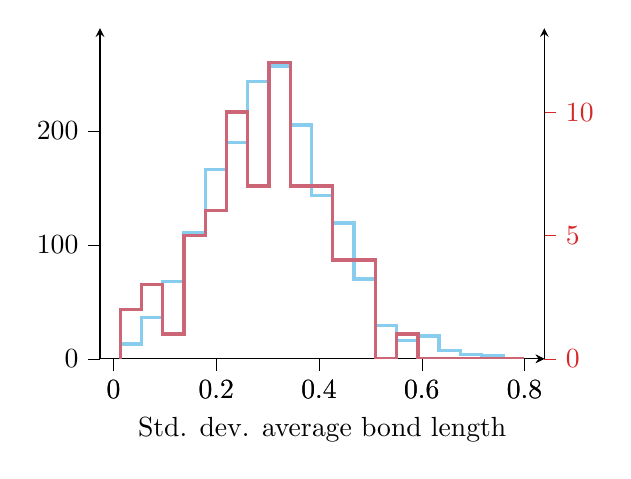
\begin{tikzpicture}

\definecolor{color0}{rgb}{0.866666666666667,0.8,0.466666666666667}
\definecolor{color1}{rgb}{0.533333333333333,0.8,0.933333333333333}
\definecolor{color2}{rgb}{0.83921568627451,0.152941176470588,0.156862745098039}
\definecolor{color3}{rgb}{0.8,0.4,0.466666666666667}

\begin{axis}[
height=2.275590092707901in,
legend cell align={left},
legend style={fill opacity=0.8, draw opacity=1, text opacity=1, draw=white!80!black},
tick align=outside,
tick pos=left,
title={},
width=2.8444876158848764in,
x grid style={white!69.0196078431373!black},
xlabel={Std. dev. average bond length},
xmin=-0.0263144046185111, xmax=0.838491250528538,
xtick style={color=black},
y grid style={white!69.0196078431373!black},
ytick style={color=black},
ylabel={},
ymin=0, ymax=290.0,
]
\path [draw=color1, very thick]
(axis cs:0.0129949433427184,0)
--(axis cs:0.0129949433427184,13)
--(axis cs:0.0543732043545389,13)
--(axis cs:0.0543732043545389,36)
--(axis cs:0.0957514653663595,36)
--(axis cs:0.0957514653663595,68)
--(axis cs:0.13712972637818,68)
--(axis cs:0.13712972637818,111)
--(axis cs:0.178507987390001,111)
--(axis cs:0.178507987390001,166)
--(axis cs:0.219886248401821,166)
--(axis cs:0.219886248401821,190)
--(axis cs:0.261264509413642,190)
--(axis cs:0.261264509413642,243)
--(axis cs:0.302642770425462,243)
--(axis cs:0.302642770425462,257)
--(axis cs:0.344021031437283,257)
--(axis cs:0.344021031437283,205)
--(axis cs:0.385399292449103,205)
--(axis cs:0.385399292449103,143)
--(axis cs:0.426777553460924,143)
--(axis cs:0.426777553460924,119)
--(axis cs:0.468155814472744,119)
--(axis cs:0.468155814472744,70)
--(axis cs:0.509534075484565,70)
--(axis cs:0.509534075484565,29)
--(axis cs:0.550912336496385,29)
--(axis cs:0.550912336496385,16)
--(axis cs:0.592290597508206,16)
--(axis cs:0.592290597508206,20)
--(axis cs:0.633668858520026,20)
--(axis cs:0.633668858520026,7)
--(axis cs:0.675047119531847,7)
--(axis cs:0.675047119531847,4)
--(axis cs:0.716425380543667,4)
--(axis cs:0.716425380543667,3)
--(axis cs:0.757803641555488,3)
--(axis cs:0.757803641555488,0)
--(axis cs:0.799181902567308,0)
--(axis cs:0.799181902567308,0);

\end{axis}

\begin{axis}[
axis y line=right,
height=2.275590092707901in,
tick align=outside,
width=2.8444876158848764in,
x grid style={white!69.0196078431373!black},
xmin=-0.0263144046185111, xmax=0.838491250528538,
xtick pos=left,
xtick style={color=black},
y grid style={white!69.0196078431373!black},
ymin=0, ymax=13.4,
ytick pos=right,
ytick style={color=color2},
yticklabel style={anchor=west, color=color2}
]
\path [draw=color3, very thick]
(axis cs:0.0129949433427184,0)
--(axis cs:0.0129949433427184,2)
--(axis cs:0.0543732043545389,2)
--(axis cs:0.0543732043545389,3)
--(axis cs:0.0957514653663595,3)
--(axis cs:0.0957514653663595,1)
--(axis cs:0.13712972637818,1)
--(axis cs:0.13712972637818,5)
--(axis cs:0.178507987390001,5)
--(axis cs:0.178507987390001,6)
--(axis cs:0.219886248401821,6)
--(axis cs:0.219886248401821,10)
--(axis cs:0.261264509413642,10)
--(axis cs:0.261264509413642,7)
--(axis cs:0.302642770425462,7)
--(axis cs:0.302642770425462,12)
--(axis cs:0.344021031437283,12)
--(axis cs:0.344021031437283,7)
--(axis cs:0.385399292449103,7)
--(axis cs:0.385399292449103,7)
--(axis cs:0.426777553460924,7)
--(axis cs:0.426777553460924,4)
--(axis cs:0.468155814472744,4)
--(axis cs:0.468155814472744,4)
--(axis cs:0.509534075484565,4)
--(axis cs:0.509534075484565,0)
--(axis cs:0.550912336496385,0)
--(axis cs:0.550912336496385,1)
--(axis cs:0.592290597508206,1)
--(axis cs:0.592290597508206,0)
--(axis cs:0.633668858520026,0)
--(axis cs:0.633668858520026,0)
--(axis cs:0.675047119531847,0)
--(axis cs:0.675047119531847,0)
--(axis cs:0.716425380543667,0)
--(axis cs:0.716425380543667,0)
--(axis cs:0.757803641555488,0)
--(axis cs:0.757803641555488,0)
--(axis cs:0.799181902567308,0)
--(axis cs:0.799181902567308,0);
\end{axis}

\end{tikzpicture}

    \subcaption{}
\end{subfigure}
\caption{Histograms of predicted suitable materials as a function of the (a) PBE-calculated band gap from Materials Project, (b) maximum ionic character, (c) standard deviation of the radial distribution function (RDF) and (d) standard deviation of the average bond length. The total number of predicted materials is  $6804$ for the Ferrenti approach, and $214$ for the empirical approach. The Ferrenti approaches refer to the left $y$-axis and the empirical approach to the right.
    }
\label{fig:histogram_new}
\end{figure}

\section*{Discussion}
Taking a closer look at the reasoning behind the choices made by the different ML methods during the classification process, we can start to identify important driving forces for manifestation of quantum compatible properties in semiconductors. 
The analysis of the principal components extracted from the ML methods revealed that the most important principal component for \mrk{the Ferrenti approach} encompasses features related to the band gap and chemical environment. This means that the band gap criterion imposed in the training set selection is at least somewhat satisfied. 
%In other words, the Ferrenti approaches appear to reproduce the logic of the initial selection process. 
\mrk{The Ferrenti approach does not entirely reproduce the logic of the initial selection process however as many low band gap materials were highlighted as suitable by the ML methods. } 
For the empirical approach, on the other hand, band gap related features were not recognized as important in the dominant principal component. 

Figure~\ref{fig:histogram_new}(a) displays the number of predicted suitable materials as a function of band gap (from the MP database), and reveals that \mrk{both} approaches predicted a substantial amount of materials with a low band gap (below $0.5$~eV). 
Moreover, the distribution of materials that were identified as suitable is rather broad with the Ferrenti \mrk{approach} exhibiting a peak around a $2.5$~eV band gap. 
Coincidentally, the band gap of, e.g., 4$H$-SiC is usually computed at around $2.5$~eV using the PBE functional. 
The empirical approach exhibits a more scattered data distribution. % with local maxima around $1$-$2$ and $4$~eV. 

The secondmost important principal component in the Ferrenti approach encompasses properties such as the ionic character, covalent radius and maximum packing efficiency (see the Supplementary Information at \cite{supplementary} for the predicted material distributions of the latter two features).  
Intriguingly, as shown in  Figure~\ref{fig:histogram_new}(b), the predicted candidates distribute over a broad range of ionic characters for \mrk{both the Ferrenti and empirical} approaches - even peaking at a relatively high ionic character of $0.8$. 
We note that this may be a result of the distribution of the initial dataset of \mrk{$25,000$} materials \mrk{with a maximum} around a similar value (not shown). The minor peak in the empirical approach's predicted materials around $0.4$ ionic character is not present for the Ferrenti approach \mrk{nor} the overall data distribution. For \mrk{reference}, all SiC entries in the dataset have maximum ionic characters of $\sim 0.1$. 
\mrk{Furthermore, the} covalent radii of the materials (see the Supplementary Information) exhibit two distinct peaks in the data distribution. 
The trend of two data peaks is repeated for the maximum packing efficiency but is much more prominent for the empirical approach. This indicates that the material density, or in other words the bond length, is an important parameter for QT suitability.  

The ML methods in the empirical approach consistently identified the first principal component as the predominant one. Identifying the single most important feature in this principal component proved challenging as it is the combined impact of several features that \mrk{matters}. 
Here, \mrk{the} standard deviation of the radial distribution function (RDF) has a  particularly strong impact since it appears four times in different forms in the top ten list over dominating features. One configuration of the standard deviation of the RDF is demonstrated in \mrk{Figure}~\ref{fig:histogram_new}(c), with two others being included in the Supplementary Information at \cite{supplementary}. Intriguingly, the standard deviation of the RDF exhibits substantial discrepancies between the \mrk{Ferrenti} and the empirical approach. For the empirical approach, there is a sharp peak in the preferred value for the standard deviation for the RDF, while the Ferrenti \mrk{approach displays} an even distribution across a broader range. 
\mrk{These observations emphasize the importance of symmetry related material properties for QT suitability. }

We interpret the standard deviation  of the RDF such that zero standard deviation in the RDF means that there is no variation in the radial symmetry throughout the material. Similarly, zero standard deviation in the average bond length would mean that all bonds are identical throughout the crystal. Intriguingly, the peaks in the distributions of the predicted materials are not found for perfectly symmetric materials with identical bond lengths; instead, some variation in the bond and wavefunction distributions is found to be optimal for a material to be suitable for QT.  
Note that the maxima in Fig.~\ref{fig:histogram_new}(c) seem to appear for moderate standard deviations in the RDF, indicating that a certain degree of symmetry is necessary for a material to act as a suitable QT host. The exact degree and type of symmetry is still open to debate and merits further study. 
Similar symmetry related features such as the standard deviation of the average bond length (see Figure~\ref{fig:histogram_new}d), the site fingerprint of the chemical environment and the bond orientation (see the Supplementary Information at \cite{supplementary}) are also influential in guiding the ML algorithms upon classifying suitable and unsuitable materials for QT in the empirical approach. 


Interestingly, none of the nine materials predicted by the empirical approach above a $0.85$ threshold, nor of the six materials predicted by all approaches to $0.75$ confidence, are elemental. At most three different elements are present, but the emphasis is clearly on binary compounds. This resonates with the observations from the principal component analysis; an optimal degree of crystalline order likely exists for a material to manifest QT compatible properties, but some variations throughout the crystal in, e.g., bond length and symmetry are needed. This is in contrast to the expectations that guided the formulation of the test and training sets in the Ferrenti \mrk{approach}. Where most previous works have highlighted features such as band gap, polarity and ionic character as vital for a semiconductor to manifest quantum compatible features, our results reveal that local variations in the crystal structure related to symmetry and bond angles, length and orientation should be considered as well and may be more important. 

Considering the trends in machine learning selectivity in light of the specific defect centers we know to be quantum compatible reveals fascinating characteristics. None of the known quantum emitters or spin centers seem to appear in completely uniform systems. For example, in the high symmetry materials of diamond and silicon, QT compatible defects are not intrinsic; neither the silicon vacancy in silicon nor the carbon vacancy in diamond, for example,  have exhibited single-photon emission or controllable spin coherence. Instead, \mrk{quantum} effects often appear after impurities are introduced, as evidenced by the phosphorous and carbon impurities in silicon \cite{He2019,Redjem2020} and the nitrogen-vacancy, germanium-vacancy, tin-vacancy and lead-vacancy centers in diamond \cite{Thiering2020}. 
For the binary system of silicon carbide in different polytypes, on the other hand, intrinsic defects like the silicon vacancy and the divacancy are appropriate for our goals. 
While these trends have yet to be verified on a grander scale, our findings provide strong indications that local variations in the crystal structure are paramount for QT compatible properties to manifest in a semiconductor host. 

\mrk{One should note that there is a certain degree of bias inherent to the data set labeled in the empirical approach. Firstly, experimental searches will always be limited by the availability and cost of materials and processing. Secondly, the discovery of the quantum compatible properties of the NV center in diamond naturally led early searchers to comparable materials such as silicon carbide. However, the broad range of materials predicted and listed in Table~\ref{tab:materialproperties} and the Supplementary Information at \cite{supplementary} indicates that the ML methods are detecting underlying properties which manifest in materials systems of several kinds. }

To summarize, the data extraction tools developed in this work resulted in a dataset of over \mrk{$25,000$} materials and more than $4800$ physics-informed features. Three different approaches (Ferrenti, extended Ferrenti and empirical) for data labeling were employed for training and testing of four ML algorithms. 
\mrk{The clear separation between suitable and unsuitable candidates after data labeling, along with the smaller number of principal components needed for obtaining optimal performance of the ML algorithms, indicate that the empirical approach based on findings from the literature is suitable for performing this type of guided search through materials databases.} 
%We find a much clearer separation between suitable and unsuitable candidates after data labeling in the empirical approach than for the two Ferrenti ones. 
%Additionally, substantially fewer principal components are needed for obtaining optimal performance of the ML algorithms for the empirical approach. 
The principal component analyses of the ML methods' performance imply that the Ferrenti \mrk{approach with its} strong focus on band gap and bonding character when assessing a material's quantum compatibility \mrk{to some extent reproduces} the specifications of the data labeling process, \mrk{as expected.} 
Valuable insight is gained from \mrk{comparing the important features of the Ferrenti with those for} the empirical approach which highlights the importance of symmetry related properties in the bond orientations and wavefunctions \mrk{over expected features related to band gap and bonding}. 

The findings presented here firmly establish that material informatics (from data mining via featurization to machine learning predictions) is a viable and important route to new discoveries in important fields. 
Our focus has been on predicting new candidate materials to host single-photon emitters and spin centers for quantum technology applications, but the \mrk{developed framework} is suitable for other fields as well. \mrk{Two possible paths are suggested to further exploit the findings presented herein.} One aspect is the pursuit of experimental verification of QT compatible effects in the materials predicted as suitable by \mrk{machine learning}. Another, perhaps even more important, route is to use the features and trends identified during the data mining and prediction process\mrk{es} to understand the distinct material characteristics that enable quantum effects to manifest, opening  thereby up for new discoveries in the field of quantum technologies. 


\section*{Methods}

\subsection*{Databases}
The Materials Project \cite{Jain2013, Jain2018} is an open-source project containing ground state properties of materials calculated using density functional theory (DFT) as implemented in the Vienna Ab initio Simulation Package (VASP) \cite{Kresse1996}. The Perdew-Burke-Ernzerhof \cite{Perdew1996} (PBE) functional is used to calculate band structures, while for transition metals, a $+U$ correction is applied to correct for correlation effects \cite{Wang2006}. The project is known as the initiator of materials genomics and offers a variety of calculated properties for over one hundred thousand inorganic crystalline materials, with frequent updates and extensions. Data extraction from Materials Project was performed in December of $2020$ for the Ferrenti and extended Ferrenti approaches, and in March $2021$ for the empirical approach. Therefore, the initial dataset for the two former approaches includes $77$ more materials than that for the empirical approach due to erroneous entries that have been removed from the Materials Project database.

The Open Quantum Materials Database (OQMD) \cite{Saal2013, Kirklin2015} contains thermodynamic and structural properties of more than $600.000$  materials. The calculations are performed with the VASP software and the electron exchange and correlation are described with the PBE functional. The $+U$ extension is included for several calculations considering specific elements \cite{Stevanovic2012}. Data extraction from OQMD was done in February of $2021$. 

JARVIS-DFT \cite{Choudhary2020} is an open-source database based on the VASP software and consists of roughly $40.000$ three-dimensional materials using the vdW-DF-OptB88 (OPT) functional \cite{Thonhauser2007, Klimes2011}. Structures included in the database are originally taken from the Materials Project \cite{Jain2013, Jain2018}, and then re-optimized using the OPT functional. Finally, the combination of the OPT and modified Becke-Johnson (mBJ) functionals \cite{Tran2009} is used to obtain a representative band gap for each structure \cite{Choudhary2018a}. Data extraction from JARVIS-DFT was done in January of $2021$, were we utilized the version made available on 30.04.2021 (see Ref. \cite{Choudhary2020}).
%at \url{figshare.com}.

The AFLOW \cite{Curtarolo2012, Curtarolo2012a, Calderon2015} repository is an automatic software framework for the calculations of a wide range of inorganic material properties. They utilize the PBE functional \mrk{with the $+U$ correction} within VASP to relax and optimize all structures from the ICSD. Data extraction was performed in the period of January to February of $2021$.

AFLOW-ML \cite{Isayev2017} is an application programming interface (API) that uses machine learning to predict thermo-mechanical and electronic properties based on the chemical composition and atomic structure alone, which are denoted as \textit{fragment descriptors}. Initially, the API decides whether a given material is a metal or an insulator, where the latter is confirmed with an additional regression method to predict the band gap. The accuracy is validated by a five-fold cross-validation process for each ML method, where they report a $93 \ \%$ prediction success of their initial binary classification method. In this work we utilized the Property Labeled Material Fragments (PLMF) openly available at their website 
(see Ref. \cite{Isayev2017}).
%\url{aflowlib.org}. 
We extract the crystallographic information files (CIF) for the crystals from Materials Project, use the CIF files as input to AFLOW-ML, which then returns an anticipated band gap. This process was executed during January of $2021$. 

\mrk{Note that from the initial criterion, we define that a material is required to have an ICSD identifier (ID) in Materials Project. This ID is included in the AFLOW,  AFLOW-ML, JARVIS-DFT and OQMD databases as well. If two different databases have different values for the same property, such as the band gap, we added both of them as columns (features) to our data to avoid any data cluttering. An additional analysis to uncover any difference in space groups reported from Materials Project and the other databases, where we had an average match of $97 \ \%$, which is close to an ideal match. We note that the small deviation might arise due to errors in either database, and is not necessarily reflected in the remaining features of the data. For the experimental values from Citrine, we could only verify the chemical formula since the experimental data is lacking information regarding the structure (e.g. space group, symmetry) of the material.}

\mrk{The data regarding a material's magnetic character is extracted from the Materials Projects database. Indeed, the majority of these calculations are based on the primitive cell, however, Materials Project performs an initial relaxation of cell and lattice parameters using a $1000$ / (number of atoms in the cell) k-point mesh to ensure that all properties calculated are representative of the idealized unit cell for each respective structure. As a result, we can find, e.g., Fe labeled as ferromagnetic and NiO as antiferromagnetic in our data set.} 

\mrk{MP includes larger structures of the same material. We have included all structures and materials from Materials Project, but we have not checked which materials are represented as a larger cell in our data. We have thereby not verified whether antiferromagnetic ordering has been investigated for all cases. This is an improvement that could be made to our method in a further work.}

\subsection*{Material Informatics}  
Matminer \cite{Ward2018} is an open source toolkit for material analysis written in Python. Matminer provides modules to extract information from a wide variety of databases. Additionally, they provide the tools to construct possibly thousands of features from calculations based on a material's composition, structure and electronic properties from DFT calculations, and have frameworks for visualization and automatic machine learning. 
To apply Matminer's featurization tools, we extend an existing implementation by \citeauthor{Breuck2021} \cite{Breuck2021}, which was used to generate a supervised machine learning framework called the MODnet. The implementation by \citeauthor{Breuck2021} provides featurization for a material's composition, structure and atomic sites. However, Matminer also provides featurization tools for a material's density of states (DOS) and band structure. Therefore, we extend their implementation to facilitate such featurizations. The features selected for featurization herein are summarized in the Supplementary Information at \cite{supplementary}. 

Pymatgen, a robust and open-source Python library for material analysis \cite{pymatgen}, was also employed to extract and generate features for several of the databases mentioned above. 

\subsection*{Machine Learning} 

Machine learning represents the science of giving computers the ability to learn without being explicitly programmed. The idea is that generic algorithms exist which can be used to find patterns in a broad class of datasets without having to write code specifically for each problem. The algorithm builds its own logic based on the data. 

The approaches to machine learning are many, but are often split into two main categories: supervised and unsupervised. In supervised learning we know the answer to a problem, and let the computer deduce the logic behind it. On the other hand, unsupervised learning is a method for identifying patterns and relationships in datasets without any prior knowledge of the system. Many researchers also operate with a third category, namely reinforcement learning. This is a paradigm of learning inspired by behavioral psychology, where learning is achieved by trial-and-error, solely from rewards and punishment. In this work our focus is on supervised learning only with labeled data for classification problems.

In this work we have applied four well-known and tested ML methods for classification problems, these are (see for example \cite{Hastie2009,Mehta2019} for discussions and applications):
\begin{enumerate}
    \item Logistic regression,
    \item Decision trees,
    \item Random forests,
    \item Gradient boosting.
\end{enumerate}
Logistic regression \cite{Hastie2009} is a simple and frequently used method for binary and multi-category classification problems. In addition to logistic regression, we have also applied and tested the predictions made by decision trees and ensemble methods like random forests and gradient boosting, the latter through the application of the computationally efficient XGBoost library \cite{xgboost2016}. Gradient boosting and random forests use decision trees as weak learners and improve their predictability. For random forests this is implemented through a collection of randomized decision trees where a subset of the features in the datasets are selected randomly when building a decision tree. Boosting methods like gradient boosting use decision trees as weak learners and improve upon these by an iterative process that involves the estimation of the gradients of the cost/loss function  \cite{Hastie2009}. Pure decision trees can easily lead to overfitting of the data under study, leading to a ML method that exhibits a high variance. Ensemble methods like random forests and gradient boosting on the other hand tend to soften the overfitting problem, resulting in both a small bias and a reduced variance of the employed method, see for example Refs.~\cite{Hastie2009,Mehta2019} for an in-depth discussion of the bias-variance trade-off in machine learning. Gradient boosting implemented through the  XGBoost library \cite{xgboost2016} is widely used by data scientists to achieve state-of-the-art results on many machine learning challenges. 

\mrk{Our findings are corroborated by the fact that all four ML methods predict a small set of the unlabeled materials as suitable, while agreeing on a large part of these materials. 
The methods we have chosen are all well tested, with random forests and gradient boosting methods tending to outperform the others, resulting normally in a small bias and variance \cite{Hastie2009,Mehta2019,Murphy2012}.}

\section*{Data availability} 
The datasets that support the findings of this study are available online at \cite{Ohebbi2021}.

\section*{Code availability} 
The codes employed to develop the machine learning results are available online at \cite{Ohebbi2021}. 

\bibliography{apssamp}

\begin{acknowledgments}

The work of LV and MEB was supported by the Research Council of Norway and the University of Oslo through the frontier research projects FUNDAMeNT (no. 251131) and QuTe (no. 325573). 
The work of MEB was supported by an ETH Zurich Postdoctoral Fellowship. 
The work of MHJ was supported by the U.S. Department of Energy, 
Office of Science, office of Nuclear Physics under grant 
No. DE-SC0021152 and U.S. National Science Foundation Grants
No. PHY-1404159 and PHY-2013047. 
The work of SGWL and ØSS was supported by the Norwegian Directorate for International Cooperation and Quality Enhancement in Higher Education (DIKU) which supports the Center for Computing in Science Education (CCSE).


\end{acknowledgments}

\section*{Author contributions}
MEB, LV and MHJ conceived the main theme of the project. OH developed the programs and performed the bulk of the work while MEB lead the writing process. All authors have contributed to the writing of the paper and the discussion and analysis of the data.

\section*{Competing interests}
The authors declare no competing interests.

\section*{Additional information}
Correspondence and requests for materials should be addressed to \url{bathen@aps.ee.ethz.ch}. 

\end{document}

